%%%%%%%%%%%%%%%%%%%% book.tex %%%%%%%%%%%%%%%%%%%%%%%%%%%%%
%
% sample root file for the chapters of your "monograph"
%
% Use this file as a template for your own input.
%
%%%%%%%%%%%%%%%% Springer-Verlag %%%%%%%%%%%%%%%%%%%%%%%%%%

% RECOMMENDED %%%%%%%%%%%%%%%%%%%%%%%%%%%%%%%%%%%%%%%%%%%%%%%%%%%
% \documentclass[graybox,envcountchap,sectrefs]{svmono}

\makeatletter
\def\input@path{{scn//}}
\makeatother

\documentclass{scndocument}

% \usepackage{mathptmx}
% \usepackage{helvet}
% \usepackage{courier}
% %
% \usepackage{type1cm}         
% \usepackage{setspace}

% \usepackage{xparse} 
% \usepackage[table]{xcolor}
% \usepackage{enumitem} 
% \usepackage{mathtools}
% \usepackage{ragged2e}
% \usepackage{float}
% \usepackage{amssymb}
% \usepackage[algo2e]{algorithm2e}
% \usepackage{algorithm}
% \usepackage{titlesec}
% \usepackage[tracking=true]{microtype}
% \usepackage{changepage}
% \usepackage{trimspaces}
% \usepackage{bm}
% \usepackage{datetime}
% \usepackage{suffix}
\usepackage{nameref}
% \usepackage[framemethod=TikZ]{mdframed}
\usepackage[normalem]{ulem}
\usepackage{longtable}
\usepackage[utf8]{inputenc}
\usepackage[T2A]{fontenc}
% \usepackage{amsmath}

\usepackage{scn}

% \renewcommand{\ULdepth}{1.8pt}

% \usepackage{makeidx}         % allows index generation
% \usepackage{graphicx}        % standard LaTeX graphics tool
%                              % when including figure files
% \graphicspath{{Figures/}}
% \usepackage{multicol}        % used for the two-column index
% \usepackage[bottom]{footmisc}% places footnotes at page bottom

\usepackage[english,main=russian]{babel}

\babelhyphenation{иден-ти-фи-ка-то-ры}

% Курсив и жирность для кириллицы
\usepackage{substitutefont}

\substitutefont{T2A}{\familydefault}{Tempora-TLF}
\makeatletter
\input{t2atempora-tlf.fd}
\DeclareFontShape{T2A}{Tempora-TLF}{m}{sc}{
    <-> ssub * Tempora-TLF/m/n
}{}

% see the list of further useful packages
% in the Reference Guide

\makeindex	       % used for the subject index
% please use the style svind.ist with
% your makeindex program

%%%%%%%%%%%%%%%%%%%%%%%%%%%%%%%%%%%%%%%%%%%%%%%%%%%%%%%%%%%%%%%%%%%%%

\usepackage{fancyhdr}
\pagestyle{fancy}
\renewcommand\headrulewidth{0pt}
\lhead{}\chead{\hspace{14.5em}{\normalfont\thepage}}\rhead{}
\cfoot{}
%\pagenumbering{arabic}
%\fancypagestyle{plain}{}
%	\fancyfoot[C]{\thepage}}
%\pagestyle{plain}

% \usepackage{geometry}
% \geometry{
%   a4paper,
%   left=20mm,
%   right=20mm,
%   top=20mm,
%   bottom=15mm,
%   %textwidth=117mm,
%   %textheight=191mm,
%   heightrounded, % <- I recommend this
%   hratio=1:1,
%   vratio=1:1,
% }

%
%DEFINES START

\newcommand{\showfont}{encoding: \f@encoding{},
  family: \f@family{},
  series: \f@series{},
  shape: \f@shape{},
  size: \f@size{}
}

\newcommand\tabsize{3em}

\newlength{\insize}
\setlength{\insize}{0.7em}

\newlength{\insizevar}
\setlength{\insizevar}{1.2em}

\newlength{\nisize}
\setlength{\nisize}{0.7em}

\newlength{\nisizevar}
\setlength{\nisizevar}{1.2em}

\newlength{\subsetsize}
\setlength{\subsetsize}{0.8em}

\newlength{\supsetsize}
\setlength{\supsetsize}{0.8em}

\newlength{\idtfsize}
\setlength{\idtfsize}{1.1em}

\newlength{\arrowsize}
\setlength{\arrowsize}{1em}

\newlength{\arrowsizevar}
\setlength{\arrowsizevar}{1.5em}

\newlength{\bulletsize}
\setlength{\bulletsize}{0.5em}

\newlength{\bulletbracketsize}
\setlength{\bulletbracketsize}{1.15em}

\newlength{\bracketsize}
\setlength{\bracketsize}{0.4em}

\newlength{\squaresize}
\setlength{\squaresize}{0.7em}

\newlength{\doublesquaresize}
\setlength{\doublesquaresize}{1.4em}

\newlength{\commentsize}
\setlength{\commentsize}{1em}

\newlength{\eqsize}
\setlength{\eqsize}{0.8em}

\newlength{\substructsize}
\setlength{\substructsize}{1.7em}

\newlength{\toclineskip}
\setlength{\toclineskip}{\baselineskip}

\newcommand{\scnsupergroupsign}{\textasciicircum}
\newcommand{\scnrolesign}{\,$^\prime$}

\newcommand{\sethind}{\setlength{\hangindent}{\dimexpr (\tabsize)*\value{hind} \relax} }
\newcommand{\sethindfromind}[1]{\setcounter{\hind}{\numexpr (\value{ind}+#1 \relax} }
\newcommand{\calctab}{\dimexpr (\tabsize)*\value{ind} \relax}
\newcommand{\settab}{\hspace{\calctab}}
\newcommand{\calcdiff}[1]{\dimexpr \tabsize-#1  \relax}
\newcommand{\makediff}[1]{\hspace{\calcdiff{#1}}}

\newcommand{\textspaced}[1]{\textls[200]{#1}}

%DEFINES END

\usepackage{tocloft}
\makeatletter
\renewcommand{\@cftmaketoctitle}{}
\makeatother
\renewcommand{\cftchapfont}{\bfseries}
\renewcommand{\cftsecfont}{\bfseries}
\renewcommand{\cftsubsecfont}{\bfseries}
\renewcommand{\cftpartleader}{\cftdotfill{\cftdotsep}}
\renewcommand{\cftchapleader}{\cftdotfill{\cftdotsep}}
\renewcommand{\cftsecleader}{\cftdotfill{\cftdotsep}}
\renewcommand{\cftsubsecleader}{\cftdotfill{\cftdotsep}}
\renewcommand{\cftsubsubsecleader}{\cftdotfill{\cftdotsep}}

\makeatletter
\renewcommand{\cftchappresnum}{\begin{lrbox}{\@tempboxa}}
\renewcommand{\cftchapaftersnum}{\end{lrbox}}
\cftsetindents{chapter}{0pt}{0pt}
\renewcommand{\cftsecpresnum}{\begin{lrbox}{\@tempboxa}}
\renewcommand{\cftsecaftersnum}{\end{lrbox}}
\cftsetindents{section}{\tabsize}{0pt}
\renewcommand{\cftsubsecpresnum}{\begin{lrbox}{\@tempboxa}}
\renewcommand{\cftsubsecaftersnum}{\end{lrbox}}
\cftsetindents{subsection}{\tabsize+\tabsize}{0pt}
\renewcommand{\cftsubsubsecpresnum}{\begin{lrbox}{\@tempboxa}}
\renewcommand{\cftsubsubsecaftersnum}{\end{lrbox}}
\cftsetindents{subsubsection}{\tabsize+\tabsize+\tabsize}{0pt}
\renewcommand{\cftparapresnum}{\begin{lrbox}{\@tempboxa}}
\renewcommand{\cftparaaftersnum}{\end{lrbox}}
\cftsetindents{paragraph}{\tabsize+\tabsize+\tabsize+\tabsize}{0pt}
\renewcommand{\cftsubparapresnum}{\begin{lrbox}{\@tempboxa}}
\renewcommand{\cftsubparaaftersnum}{\end{lrbox}}
\cftsetindents{subparagraph}{\tabsize+\tabsize+\tabsize+\tabsize+\tabsize}{0pt}
\renewcommand\cftchapafterpnum{\vspace{\toclineskip}}
\renewcommand\cftsecafterpnum{\vspace{\toclineskip}}
\renewcommand\cftsubsecafterpnum{\vspace{\toclineskip}}
\renewcommand\cftsubsubsecafterpnum{\vspace{\toclineskip}}
\renewcommand\cftparaafterpnum{\vspace{\toclineskip}}
\renewcommand\cftsubparaafterpnum{\vspace{\toclineskip}}
\makeatother

%SCN START

\usepackage{calc}

\newif\iffilemode
\filemodefalse

\makeatletter

\newcommand*{\trim}[1]{%
  \trim@spaces@noexp{#1}%
}

\newcounter{ind}
\newcounter{hind}
\newcounter{seg}
\newcounter{list_depth}

\newenvironment{SCn}{
\setcounter{ind}{0}
\setcounter{hind}{0} 
\setcounter{list_depth}{0}
\begin{flushleft}
}
{
\end{flushleft}
}

\newcommand{\scnheader}[1]{\scnresetlevel\sethind~\vspace{\parskip}\\
\textit{\textbf{#1}}\\}

\newcommand{\scnstructheader}[1]{\scnresetlevel\sethind~\vspace{\parskip}\\
\textit{\textbf{\textspaced{#1}}}\\}

\newcommand{\scnheaderlocal}[1]{\settab\textit{\textbf{#1}}\\}

\newcommand{\scnstructheaderlocal}[1]{\settab\textit{\textbf{\textspaced{#1}}}\\}

\newcommand{\scnstructidtf}[1]{\textit{\textspaced{#1}}}

\newcommand{\scnkeyword}[1]{\textit{\textbf{#1}}}

\newcommand{\scnsectionheader}[1]{\setcounter{seg}{0} \textspaced{\scnheader{\large #1}}}

\newcommand{\scnsegmentheader}[1]{
\addtocounter{seg}{1}
\ifnum\value{seg}>1
%\newpage
\bigskip
\bigskip
\else
\bigskip
\fi
\scnsegmentcaption \textspaced{\scnheader{#1}}
}

\newcommand{\scnfragmentheader}[1]{
\bigskip
\scnfragmentcaption \textspaced{\scnheader{#1}}
}

\newcommand{\scnsegmentheaderbeginning}[1]{
	\addtocounter{seg}{1}
	\ifnum\value{seg}>1
%	\newpage
	\bigskip
	\else
	\bigskip
	\fi
	\scnsegmentcaptionbeginning \textspaced{\scnheader{#1}}
}

\newcommand{\scnfragmentcaptiontext}[1]{
\begin{adjustwidth}{\commentsize}{0.5\textwidth+\commentsize}
	\justify
	\setlength{\parskip}{0.5em}
	\hspace{-\commentsize}\bfseries /*~#1~\filldots/\normalfont	
\end{adjustwidth}}

\newcommand{\scnfragmentcaption}{\bfseries /*\filldots/\hspace{\textwidth}\normalfont\vspace{\afterseglength}}

\makeatletter
\newcommand{\scnsegmentcaption}{\normalfont \bfseries /*~\textspaced{Сегмент}~\filldots/\hspace{\textwidth}\normalfont\vspace{\afterseglength}}
\makeatother

\NewDocumentCommand\scnlist{>{\SplitList{;}}m}
   {\ProcessList{#1}{\scnlistitem}}

\NewDocumentCommand\scnrellist{>{\SplitList{;}}m}
   {\ProcessList{#1}{\scnrellistitem}}

\NewDocumentCommand\scnrolerellist{>{\SplitList{;}}m}
   {\ProcessList{#1}{\scnrolerellistitem}}
   
\NewDocumentCommand\scnvarrellist{>{\SplitList{;}}m}
   {\ProcessList{#1}{\scnvarrellistitem}}
   
\NewDocumentCommand\scnvarrolerellist{>{\SplitList{;}}m}
   {\ProcessList{#1}{\scnvarrolerellistitem}}

\NewDocumentCommand\scnfilelist{>{\SplitList{;}}m}
   {\ProcessList{#1}{\scnfilelistitem}}

\NewDocumentCommand\scnlistbrackets{>{\SplitList{;}}m}
   {\ProcessList{#1}{\scnlistitembrackets}}

\NewDocumentCommand\scnfilelistbrackets{>{\SplitList{;}}m}
   {\ProcessList{#1}{\scnfilelistitembrackets}}

\newcommand\scnlistitem[1]{
\sethind
\settab{$\bullet$\makediff{\bulletsize}\itshape#1} \\
}

\newcommand\scnvarrellistitem[1]{{\textit{#1}*{\normalfont::~}}}

\newcommand\scnvarrolerellistitem[1]{{\textit{#1}\scnrolesign{\normalfont::~}}}

\newcommand\scnrellistitem[1]{{\textit{#1}*{\normalfont:~}}}

\newcommand\scnrolerellistitem[1]{{\textit{#1}\scnrolesign{\normalfont:~}}}

\newcommand\scnlistitembrackets[1]{
\sethind
\settab\hspace{0.2em}\hspace{\bracketsize}{$\bullet$\makediff{\bulletbracketsize}\itshape#1}\\
}

\newcommand\scnfilelistitembrackets[1]{
\addtocounter{hind}{1}
\begin{adjustwidth}{\calctab+\tabsize+\bracketsize}{0em}
\justify
\setlength{\parskip}{0.5em}
\hspace{-\tabsize}\hspace{0.2em}\normalfont$\bullet$\makediff{\bulletbracketsize}[#1]
\setlength{\parskip}{\baselineskip}
\end{adjustwidth}
\addtocounter{hind}{-1}
}

\newcommand\scnfilelistitem[1]{
\addtocounter{hind}{1}
\begin{adjustwidth}{\calctab+\tabsize+\bracketsize}{0em}
\justify
\setlength{\parskip}{0.5em}
\hspace{-\tabsize}\hspace{-\bracketsize}\normalfont$\bullet$\makediff{\bulletsize}[#1]
\setlength{\parskip}{\baselineskip}
\end{adjustwidth}
\addtocounter{hind}{-1}
}

\newcommand\scnfileitem[1]{\scnaddlevel{1}\scnfilelong{#1}\scnaddlevel{-1}}

\newcommand\scgfileitem[1]{\scnaddlevel{1}\scnfilescg{#1}\scnaddlevel{-1}}

\newcommand{\scnrelfrom}[2]{
\settab$\bm{\Rightarrow}$\makediff{\arrowsize}\scnrellist{#1}\\
\addtocounter{ind}{1}
\sethindfromind{1}
\sethind
\settab{\itshape#2}\\
\addtocounter{ind}{-1}
\sethindfromind{1}
}

\newcommand{\scnrelsuperset}[2]{
\settab$\bm{\supset}$\makediff{\supsetsize}\scnrellist{#1}\\
\addtocounter{ind}{1}
\sethindfromind{1}
\sethind
\settab{\itshape#2}\\
\addtocounter{ind}{-1}
\sethindfromind{1}
}

\newcommand{\scnvarrelfrom}[2]{
	\settab\textunderscore$\bm{\Rightarrow}$\makediff{\arrowsizevar}\scnvarrellist{#1}\\
	\addtocounter{ind}{1}
	\sethindfromind{1}
	\sethind
	\settab{\itshape #2}\\
	\addtocounter{ind}{-1}
	\sethindfromind{1}
}

\newcommand{\scnrelto}[2]{
\settab$\bm{\Leftarrow}$\makediff{\arrowsize}\scnrellist{#1}\\
\addtocounter{ind}{1}
\sethindfromind{1}
\sethind 
\settab{\itshape #2}\\
\addtocounter{ind}{-1}
\sethindfromind{1}
}

\newcommand{\scnvarrelto}[2]{
\settab\textunderscore$\bm{\Leftarrow}$\makediff{\arrowsizevar}\scnvarrellist{#1}\\
\addtocounter{ind}{1}
\sethindfromind{1}
\sethind 
\settab{\itshape #2}\\
\addtocounter{ind}{-1}
\sethindfromind{1}
}

\newcommand{\scnrelfromlist}[2]{
\settab$\bm{\Rightarrow}$\makediff{\arrowsize}\scnrellist{#1}\\
\addtocounter{ind}{1}
\addtocounter{hind}{1}
\addtocounter{list_depth}{1}
\ifnum\value{list_depth}=1
	\addtocounter{hind}{1}
\fi
\sethind 

\iffilemode
\scnfilelist{#2}
\else
\scnlist{#2}
\fi

\addtocounter{ind}{-1}
\ifnum\value{list_depth}=1
	\addtocounter{hind}{-1}
\fi
\addtocounter{list_depth}{-1}
\addtocounter{hind}{-1}
}

\newcommand{\scnreltolist}[2]{
\settab$\bm{\Leftarrow}$\makediff{\arrowsize}\scnrellist{#1}\\
\addtocounter{ind}{1}
\addtocounter{hind}{1}
\addtocounter{list_depth}{1}
\ifnum\value{list_depth}=1
	\addtocounter{hind}{1}
\fi
\sethind 

\iffilemode
\scnfilelist{#2}
\else
\scnlist{#2}
\fi

\addtocounter{ind}{-1}
\ifnum\value{list_depth}=1
	\addtocounter{hind}{-1}
\fi
\addtocounter{list_depth}{-1}
\addtocounter{hind}{-1}
}

\newcommand{\scnrelboth}[2]{
\settab$\bm{\Leftrightarrow}$\makediff{\arrowsize}\scnrellist{#1}\\
\addtocounter{ind}{1}
\addtocounter{hind}{1}
\sethind 
\settab{\itshape #2} \\
\addtocounter{hind}{-1}
\addtocounter{ind}{-1}
}

\newcommand{\scnrelbothlist}[2]{
\settab$\bm{\Leftrightarrow}$\makediff{\arrowsize}\scnrellist{#1}\\
\addtocounter{ind}{1}
\addtocounter{hind}{2}
\sethind 

\iffilemode
\scnfilelist{#2}
\else
\scnlist{#2}
\fi

\addtocounter{ind}{-1}
\addtocounter{hind}{-2}
}

\newcommand{\scnrelfromcommonset}[4]{
\settab$\bm{\Rightarrow}$\makediff{\arrowsize}\scnrellist{#3}\\
\addtocounter{ind}{1}
\addtocounter{hind}{1}
\addtocounter{list_depth}{1}
\ifnum\value{list_depth}=1
	\addtocounter{hind}{1}
\fi
\sethind 

\settab#1\\
\iffilemode
\vspace{-1.55\baselineskip}
\scnfilelistbrackets{#4}
\else
\vspace{-1\baselineskip}
\scnlistbrackets{#4}
\fi
\settab#2\\

\addtocounter{ind}{-1}
\ifnum\value{list_depth}=1
	\addtocounter{hind}{-1}
\fi
\addtocounter{list_depth}{-1}
\addtocounter{hind}{-1}
}

\newcommand{\scnrelfromset}[2]{\scnrelfromcommonset{$\pmb{\{}$}{$\pmb{\}}$}{#1}{#2}}

\newcommand{\scnrelfromvector}[2]{\scnrelfromcommonset{$\pmb{\langle}$}{$\pmb{\rangle}$}{#1}{#2}}

\newcommand{\scnreltocommonset}[4]{
\settab$\bm{\Leftarrow}$\makediff{\arrowsize}\scnrellist{#3}\\
\addtocounter{ind}{1}
\addtocounter{hind}{1}
\addtocounter{list_depth}{1}
\ifnum\value{list_depth}=1
	\addtocounter{hind}{1}
\fi
\sethind 

\settab#1\\
\iffilemode
\vspace{-1.55\baselineskip}
\scnfilelistbrackets{#4}
\else
\vspace{-1\baselineskip}
\scnlistbrackets{#4}
\fi
\settab#2\\

\addtocounter{ind}{-1}
\ifnum\value{list_depth}=1
	\addtocounter{hind}{-1}
\fi
\addtocounter{list_depth}{-1}
\addtocounter{hind}{-1}
}

\newcommand{\scnreltoset}[2]{\scnreltocommonset{$\pmb{\{}$}{$\pmb{\}}$}{#1}{#2}}

\newcommand{\scnreltovector}[2]{\scnreltocommonset{$\pmb{\langle}$}{$\pmb{\rangle}$}{#1}{#2}}

\newcommand{\scneq}[1]{
\addtocounter{hind}{1}
\sethind 
\settab$\bm{=}$\makediff{\eqsize}{\itshape #1}\\
\addtocounter{hind}{-1}
}

\newcommand{\scneqfile}[1]{
\settab$\bm{=}$\\ 
\vspace{0.5\baselineskip}
\scnfilelong{#1}
}

\newcommand{\scneqimage}[1]{
\settab$\bm{=}$\\ 
\vspace{0.5\baselineskip}
\scnfileimage{#1}
}

\newcommand{\scneqtable}[1]{
\settab$\bm{=}$\\ 
\vspace{0.5\baselineskip}
\scnfiletable{#1}
}

\newcommand{\scneqscg}[1]{
\settab$\bm{=}$\\ 
\vspace{0.5\baselineskip}
\scnfilescg{#1}
}

\newcommand{\scneqfileclass}[1]{
\settab$\bm{=}$\makediff{\eqsize}\scnfileclass{#1}\\
}

\newcommand{\scneqtocommonset}[3]{
\settab$\bm{=}$\makediff{\eqsize}#1\\
\addtocounter{ind}{1}
\addtocounter{hind}{1}
\addtocounter{list_depth}{1}
\ifnum\value{list_depth}=1
\addtocounter{hind}{1}
\fi
\sethind 

\iffilemode
\vspace{-1.55\baselineskip}
\scnfilelistbrackets{#3}
\else
\vspace{-1\baselineskip}
\scnlistbrackets{#3}
\fi
\settab#2\\

\addtocounter{ind}{-1}
\ifnum\value{list_depth}=1
\addtocounter{hind}{-1}
\fi
\addtocounter{list_depth}{-1}
\addtocounter{hind}{-1}
}

\newcommand{\scneqtoset}[1]{\scneqtocommonset{$\pmb{\{}$}{$\pmb{\}}$}{#1}}

\newcommand{\scneqtovector}[1]{\scneqtocommonset{$\pmb{\langle}$}{$\pmb{\rangle}$}{#1}}

\newcommand{\scnhassubstruct}[1]{
\settab$\bm{\supset=}$\makediff{\substructsize}$\pmb{\{}$\\
\addtocounter{ind}{1}
\addtocounter{hind}{2}
\sethind 
\iffilemode
\vspace{-1.55\baselineskip}
\scnfilelistbrackets{#1}
\else
\vspace{-1\baselineskip}
\scnlistbrackets{#1}
\fi
\settab$\pmb{\}}$\\
\addtocounter{ind}{-1}
\addtocounter{hind}{-2}
}

\newcommand{\scnsubset}[1]{
\addtocounter{hind}{1}
\sethind 
\settab$\bm{\subset}$\makediff{\subsetsize}{\itshape #1}\\
\addtocounter{hind}{-1}
}

\newcommand{\scnnotsubset}[1]{
\addtocounter{hind}{1}
\sethind 
\settab$\bm{\not\subset}$\makediff{\subsetsize}{\itshape #1}\\
\addtocounter{hind}{-1}
}

\newcommand{\scnsuperset}[1]{
\addtocounter{hind}{1}
\sethind 
\settab$\bm{\supset}$\makediff{\supsetsize}{\itshape #1}\\
\addtocounter{hind}{-1}
}

\newcommand{\scniselement}[1]{
\addtocounter{hind}{1}
\sethind
\settab$\bm{\in}$\hspace{\calcdiff{\insize}}{\itshape #1}\\
\addtocounter{hind}{-1}
}

\newcommand{\scnisvarelement}[1]{
	\addtocounter{hind}{1}
	\sethind
	\settab\textunderscore$\bm{\in}$\makediff{\insizevar}{\itshape #1}\\
	\addtocounter{hind}{-1}
}

\newcommand{\scnmakecommonsetlocal}[3]{
\hspace{-\bracketsize}#1\\
\addtocounter{ind}{1}
\addtocounter{hind}{2}
\sethind 
\vspace{-1\baselineskip}
\scnlistbrackets{#3}
\settab#2\\
\addtocounter{ind}{-1}
\addtocounter{hind}{-2}
}

\newcommand{\scnmakesetlocal}[1]{\scnmakecommonsetlocal{$\pmb{\{}$}{$\pmb{\}}$}{#1}}

\newcommand{\scnmakevectorlocal}[1]{\scnmakecommonsetlocal{$\pmb{\langle}$}{$\pmb{\rangle}$}{#1}}

\newcommand{\scnmakeset}[1]{
\settab$\pmb{\{}$\\
\sethind 
\vspace{-1\baselineskip}
\scnlistbrackets{#1}
\settab$\pmb{\}}$\\
}

\newcommand{\scnhaselementset}[1]{
\settab$\bm{\ni}$\makediff{\nisize}\scnmakesetlocal{#1}
}

\newcommand{\scnhaselementvector}[1]{
\settab$\bm{\ni}$\makediff{\nisize}\scnmakevectorlocal{#1}
}

\newcommand{\scnhaselement}[1]{
\addtocounter{hind}{1}
\sethind 
\settab$\bm{\ni}$\makediff{\nisize}{\itshape #1}\\
\addtocounter{hind}{-1}
}

\newcommand{\scnhasvarelement}[1]{
\addtocounter{hind}{1}
\sethind 
\settab\textunderscore$\bm{\ni}$\makediff{\nisizevar}{\itshape #1}\\
\addtocounter{hind}{-1}
}

\newcommand{\scnhaselements}[1]{
\addtocounter{hind}{1}
\sethind 
\settab$\bm{\ni}$\makediff{\nisize}#1\\
\addtocounter{hind}{-1}
}

\newcommand{\scnsubdividing}[1]{\scnrelfromset{разбиение}{#1}}

\newcommand{\scnhaselementrole}[2]{
\settab$\bm{\ni}$\makediff{\nisize}\scnrolerellist{#1}\\
\addtocounter{ind}{1}
\addtocounter{hind}{1}
\sethind 
\settab{\itshape #2}\\
\addtocounter{ind}{-1}
\addtocounter{hind}{-1}
}

\newcommand{\scnhasvarelementrole}[2]{
	\settab\textunderscore$\bm{\ni}$\makediff{\nisizevar}\scnvarrolerellist{#1}\\
	\addtocounter{ind}{1}
	\addtocounter{hind}{1}
	\sethind 
	\settab{\itshape #2}\\
	\addtocounter{ind}{-1}
	\addtocounter{hind}{-1}
}

\newcommand{\scnhaselementlist}[2]{
\settab$\bm{\ni}$\makediff{\nisize}\scnrolerellist{#1}\\
\addtocounter{ind}{1}
\addtocounter{hind}{2}
\sethind 
\scnlist{#2}
\addtocounter{ind}{-1}
\addtocounter{hind}{-2}
}

\newcommand{\scniselementrole}[2]{
\settab$\bm{\in}$\makediff{\insize}\scnrolerellist{#1}\\
\addtocounter{ind}{1}
\addtocounter{hind}{1}
\sethind 
\settab{\itshape #2}\\
\addtocounter{ind}{-1}
\addtocounter{hind}{-1}
}

\newcommand{\scniselementlist}[2]{
\settab$\bm{\in}$\makediff{\nisize}\scnrolerellist{#1}\\
\addtocounter{ind}{1}
\addtocounter{hind}{2}
\sethind 
\scnlist{#2}
\addtocounter{ind}{-1}
\addtocounter{hind}{-2}
}

\newcommand{\scnrole}[1]{{\itshape #1\scnrolesign}:}

\newcommand{\scnset}[1]{$\pmb{\{}$#1$\pmb{\}}$}
\newcommand{\scnvector}[1]{$\pmb{\langle}$#1$\pmb{\rangle}$}

\newcommand{\scnidtf}[1]{
\addtocounter{hind}{1}
\begin{adjustwidth}{\calctab+\tabsize+\bracketsize}{0em}
\justify
\setlength{\parindent}{0em}
\setlength{\itemindent}{0em}
\setlength{\parskip}{0.5em}
\vspace{-0.4\baselineskip}
\hspace{-\tabsize}\hspace{-\bracketsize}\normalfont$\bm{\coloneqq}$\makediff{\idtfsize}[#1]
\end{adjustwidth}
\addtocounter{hind}{-1}
}

\newcommand{\scnidtftext}[2]{
\settab$\bm{\coloneqq}$\hspace{\calcdiff{\idtfsize}}\scnrellist{#1}\\
\addtocounter{ind}{1}
\settab{\scnfilelong{#2}}\\
\addtocounter{ind}{-1}
}

\newcommand{\scnidtfdef}[1]{\scnidtftext{определение}{#1}}

\newcommand{\scnidtfexp}[1]{\scnidtftext{пояснение}{#1}}

\newcommand{\scnaddlevel}[1]{
\addtocounter{ind}{#1}
\addtocounter{hind}{#1}}

\newcommand{\scnaddhind}[1]{
\addtocounter{hind}{#1}}

\newcommand{\scnresetlevel}{
\setcounter{ind}{0}
\setcounter{hind}{0}}

\newcommand{\scnfileshort}[1]{
{\normalfont [#1]}
}

\newcommand{\scnfileclass}[1]{
{\normalfont\hspace{-0.3em}![~#1~]!}
}

\newcommand{\scnfilelong}[1]{
\begin{adjustwidth}{\calctab+0.4em}{0em}
\justify
\setlength{\parindent}{0em}
\setlength{\itemindent}{0em}
\setlength{\parskip}{0.5em}
\vspace{-1.5em}
\hspace{-0.4em}\normalfont \textbf{[}#1\textbf{]}
\end{adjustwidth}
}

\newcommand{\scnexternalfile}[1]{
\begin{adjustwidth}{\calctab+0.4em}{0em}
\justify
\setlength{\parindent}{0em}
\setlength{\itemindent}{0em}
\setlength{\parskip}{0.5em}
\vspace{-1.5em}
\normalfont#1
\end{adjustwidth}
}

\usepackage{tabularx}

\newcommand{\scnfileimage}[1]{
\begin{adjustwidth}{\calctab}{0em}
\setlength{\parindent}{0em}
\setlength{\itemindent}{0em}
\setlength{\parskip}{0.5em}
\vspace{-1.5em}
\normalfont \textbf{[}
\setlength\arrayrulewidth{1pt}
\hspace{0.1em}\begin{tabularx}{\textwidth-\calctab}{X}
\cellcolor{white}\begin{center}\vspace{-1.3\baselineskip}#1\vspace{-0.7\baselineskip}\end{center}
\end{tabularx}
\textbf{]}
\end{adjustwidth}
}

\newcommand{\scnfiletable}[1]{
\begin{adjustwidth}{\calctab}{0em}
\setlength{\parindent}{0em}
\setlength{\itemindent}{0em}
\setlength{\parskip}{0.5em}
\vspace{-1.5em}
\normalfont \textbf{[}
\rowcolors{1}{white}{white}
#1
\textbf{]}
\end{adjustwidth}
}

\newcommand{\scnfilescg}[1]{
\begin{adjustwidth}{\calctab}{0em}
\setlength{\parindent}{0em}
\setlength{\itemindent}{0em}
\setlength{\parskip}{0.5em}
\vspace{-1.5em}
\normalfont \textbf{[}
\setlength\arrayrulewidth{1pt}
\hspace{0.1em}\begin{tabularx}{\textwidth-\calctab}{X}
\cellcolor{white}\begin{center}\vspace{-1.3\baselineskip}\includegraphics[scale=0.8]{#1}\vspace{-0.7\baselineskip}\end{center}
\end{tabularx}
\textbf{]}
\end{adjustwidth}
}

\newcommand{\scnfilescn}[1]{
	\begin{adjustwidth}{\calctab}{0em}
		\setlength{\parindent}{0em}
		\setlength{\itemindent}{0em}
		\setlength{\parskip}{0.5em}
		\vspace{-1.5em}
		\normalfont \textbf{[}
		#1
		\textbf{]}
	\end{adjustwidth}
}

\newcommand{\scnstartsubstruct}{
\settab$\pmb{\supset=}$\\
\settab$\pmb{\{}$
}

\newcommand{\scnstructinclusion}{
\settab$\pmb{\supset=}$\\
}

\newcommand{\scnstartstruct}{\settab$\pmb{=\{}$}
\newcommand{\scnstartset}{\settab$\pmb{\{}$}
\newcommand{\scnstartsetlocal}{$\pmb{\{}$}
\newcommand{\scnendstruct}{\settab$\pmb{\}}$}

\newcommand{\scnendstructlocal}{$\pmb{\}}$}

\newcommand{\scnstartfile}{\settab\textbf{=}\\
\settab\textbf{[}\\}

\newcommand{\scnendfile}{\settab\textbf{]}}


\newcommand{\scnfilelongbreaks}[1]
{\scnfilelong{\\#1\\}}

\newcommand{\scntext}[2]{
\scnrelfrom{#1}{\scnfilelong{#2}}
}

\newcommand{\scneqhierstruct}{
\settab$\pmb{=\langle|}$}

\newcommand{\scnstarthierstruct}{\settab$\pmb{\langle|}$}
\newcommand{\scnendhierstruct}{\settab$\pmb{|\rangle}$}

\newcommand{\scncomment}[1]{
\scntext{комментарий}{#1}
}

\newcommand{\scnexplanation}[1]{
\scntext{пояснение}{#1}
}

\newcommand{\scnnote}[1]{
\scntext{примечание}{#1}
}

\newcommand{\scndefinition}[1]{
\scntext{определение}{#1}
}

\newcommand{\scnevolution}[1]{
\scntext{эволюция}{#1}
}

\newcommand{\scnproblems}[1]{
\scntext{проблемы}{#1}
}

\newcommand{\scnevolutiondirections}[1]{
\scntext{направления эволюции}{#1}
}

\newcommand{\scnevolutionproblems}[1]{
\scntext{проблемы развития}{#1}
}

\newcommand{\scnmodernstate}[1]{
\scntext{современное состояние}{#1}
}

\newcommand{\scnsolutionapproach}[1]{
\scntext{предлагаемый подход к решению}{#1}
}

\newcommand{\scnadvantages}[1]{
\scntext{достоинства}{#1}
}

\newcommand{\scnprinciples}[1]{
\scntext{принципы}{#1}
}

\newcommand{\scnspheresapplication}[1]{
\scntext{сферы применения}{#1}
}

\newcommand{\scnseminclusion}[1]{
\scntext{семантическое включение}{#1}
}

\newcommand{\scneditor}[1]{
\scnrelfrom{редактор}{#1}
}

\newcommand{\scneditors}[1]{
\scnrelfromlist{редактор}{#1}
}

\newcommand{\scnsourcecomment}[1]{{\normalfont \normalsize \textbf{/*~}#1\textbf{{}~*/}}}

\newcommand{\scnsourcecommentpar}[1]{
\begin{adjustwidth}{\calctab+1em}{0em}
\justify
\setlength{\parindent}{0em}
\setlength{\itemindent}{0em}
\hspace{-1em}\normalfont /*~#1{}~*/
\end{adjustwidth}
}

\newcommand{\scninlinesourcecommentpar}[1]{
\begin{adjustwidth}{\calctab+1em+\tabsize}{0em}
\justify
\setlength{\parindent}{0em}
\setlength{\itemindent}{0em}
\vspace{-0.9\baselineskip}
\hspace{-1em}\normalfont /*~#1{}~*/
\end{adjustwidth}
}

\makeatletter
\newcommand{\scnendcurrentsectioncomment}{
\scninlinesourcecommentpar{Завершили Раздел ``\textit{\@currentlabelname}''}
}
\makeatother

\newcommand{\scnendsegmentcomment}[1]{
	\scninlinesourcecommentpar{Завершили Сегмент ``\textit{#1}''}
}

\newcommand{\scnendfragmentcomment}{\\
{\bfseries \normalsize /*\filldots/\hspace{0.5\textwidth}}
}

\newcommand{\scnauthorcomment}[1]{\begin{flushleft}
/*/*#1*/*/\end{flushleft}}

\newenvironment{FileFrame}{
\begin{mdframed}[linewidth=0.5mm,roundcorner=0pt]
}
{
\end{mdframed}
}

\newenvironment{ContourFrame}{
\begin{mdframed}[linewidth=0.5mm,roundcorner=20pt]
}
{
\end{mdframed}
}

%Subject domains
\newcommand{\scnsdmainclass}[1]{
\scnhaselementlist{максимальный класс объектов исследования}{#1}
}

\newcommand{\scnsdmainclasssingle}[1]{
\scnhaselementrole{максимальный класс объектов исследования}{#1}
}

\newcommand{\scnsdclass}[1]{
\scnhaselementlist{класс объектов исследования}{#1}
}

\newcommand{\scnsdrelation}[1]{
\scnhaselementlist{исследуемое отношение}{#1}
}

%Developer info

\newcommand{\timestamp}{\vspace{0.5em}\scnauthorcomment{\textbf{\large Версия от \today~ \currenttime}}}

\newcommand{\addedstart}{\reversemarginpar\marginpar{\hspace{3em}НОВОЕ~[}}

\newcommand{\addedend}{\reversemarginpar\marginpar{\hspace{3em}]~НОВОЕ}}

\newcommand{\editedstart}{\reversemarginpar\marginpar{\hspace{3em}ИЗМЕНЕНО~[}}

\newcommand{\editedend}{\reversemarginpar\marginpar{\hspace{3em}]~ИЗМЕНЕНО}}

\newcommand{\scnbigspace}{~~}

\makeatother

%SCN END

%Sections START

\titleformat{\chapter}[display]
{\normalfont\bfseries}{}{0pt}{\normalsize}

\titleformat{\section}[display]
{\normalfont\bfseries}{}{0pt}{\normalsize}

\titleformat{\subsection}[display]
{\normalfont\bfseries}{}{0pt}{\normalsize}

\titleformat{\subsubsection}[display]
{\normalfont\bfseries}{}{0pt}{\normalsize}

\titleformat{\paragraph}[display]
{\normalfont\bfseries}{}{0pt}{\normalsize}

\titlespacing*{\chapter}
{0em}{0em}{0em}
\titlespacing*{\section}
{0em}{0em}{0em}
\titlespacing*{\subsection}
{0em}{0em}{0em}
\titlespacing*{\subsubsection}
{0em}{0em}{0em}
\titlespacing*{\paragraph}
{0em}{0em}{0em}

\newcommand{\filldots}{\xleaders\hbox{*}\hfill}
\newlength\afterparlength
\setlength{\afterparlength}{-2em}

\newlength\afterseglength
\setlength{\afterseglength}{-1em}

\newcommand{\scsuperchapter}{{\normalfont\bfseries\large/*\filldots/}\vspace{0.5\afterparlength}}

\newcommand{\scchapter}[2][]{\clearpage\chapter[\textit{#2}]{/*~\textspaced{\large Раздел}~\filldots/\vspace{\afterparlength}}
\ifx&#1&
\else
\addtocontents{toc}{\vspace{\dimexpr -\toclineskip-0.4\baselineskip \relax}\parbox{\textwidth}{\begin{SCn}\protect#1\end{SCn}}
\vspace{\toclineskip}}
\fi}

\newcommand{\scsection}[2][]{\clearpage
\section[\textit{#2}]{/*~\textspaced{\large Раздел}~\filldots/\vspace{\afterparlength}}
\ifx&#1&
\else
\addtocontents{toc}{\vspace{\dimexpr -\toclineskip+0.1\baselineskip \relax}\parbox{\textwidth}{\begin{adjustwidth}{\tabsize}{0em}\begin{SCn}\protect#1\end{SCn}\end{adjustwidth}}
\vspace{\toclineskip}}
\fi}

\newcommand{\scseparatedfragment}[2][]{\clearpage\chapter[\textit{#2}]{/*\filldots/\vspace{\afterparlength}}
\ifx&#1&
\else
\addtocontents{toc}{\vspace{\dimexpr -\toclineskip-0.4\baselineskip \relax}\parbox{\textwidth}{\begin{SCn}\protect#1\end{SCn}}
\vspace{\toclineskip}}
\fi}

\newcommand\scsubsection[2][]{\clearpage
\subsection[\textit{#2}]{/*~\textspaced{\large Раздел}~\filldots/\vspace{\afterparlength}}
\ifx&#1&
\else
\addtocontents{toc}{\vspace{\dimexpr -\toclineskip+0.1\baselineskip \relax}\parbox{\textwidth}{\begin{adjustwidth}{\tabsize+\tabsize}{0em}\begin{SCn}\protect#1\end{SCn}\end{adjustwidth}}
\vspace{\toclineskip}}
\fi}

\newcommand{\scsubsubsection}[2][]{\clearpage
\subsubsection[\textit{#2}]{/*~\textspaced{\large Раздел}~\filldots/\vspace{\afterparlength}}
\ifx&#1&
\else
\addtocontents{toc}{\vspace{\dimexpr -\toclineskip+0.1\baselineskip \relax}\parbox{\textwidth}{\begin{adjustwidth}{\tabsize+\tabsize+\tabsize}{0em}\begin{SCn}\protect#1\end{SCn}\end{adjustwidth}}
\vspace{\toclineskip}}
\fi}

\newcommand{\scparagraph}[2][]{\clearpage\paragraph[\textit{#2}]{/*~\textspaced{\large Раздел}~\filldots/\vspace{\afterparlength}}
\ifx&#1&
\else
\addtocontents{toc}{\vspace{\dimexpr -\toclineskip+0.1\baselineskip \relax}\parbox{\textwidth}{\begin{adjustwidth}{\tabsize+\tabsize+\tabsize+\tabsize}{0em}\begin{SCn}\protect#1\end{SCn}\end{adjustwidth}}
\vspace{\toclineskip}}
\fi}

\makeatletter
\newcommand*{\currentname}{\@currentlabelname}
\makeatother

\makeatletter
\newcommand*{\currentnumber}{\@currentlabel}
\makeatother

%Sections END

% Itemize START

\newenvironment{scnitemize}{
\begin{itemize}[leftmargin=\leftmargin-1em+\bracketsize,itemsep=-0.25em,before=\vspace{-0.8em},after=\vspace{-0.5em}]
\renewcommand{\labelitemi}{\scriptsize$\square$}
\renewcommand{\labelitemii}{\scriptsize$\square~\square$}
\renewcommand{\labelitemiii}{\scriptsize$\square~\square~\square$} 
}
{
\end{itemize}
}

\newenvironment{scnitemizeii}{
\begin{itemize}[leftmargin=\leftmargin-1em+\bracketsize+\squaresize,itemsep=-0.25em,before=\vspace{-0.3em},after=\vspace{0em}]
\renewcommand{\labelitemi}{\scriptsize$\square~\square$} 
}
{
\end{itemize}
}

\newenvironment{scnitemizeiii}{
\begin{itemize}[leftmargin=\leftmargin-1em+\bracketsize+\doublesquaresize,itemsep=-0.25em,before=\vspace{-0.3em},after=\vspace{0em}]

\renewcommand{\labelitemi}{\scriptsize$\square~\square$} 
}
{
\end{itemize}
}

\newenvironment{scnenumerate}{
\begin{enumerate}[leftmargin=\leftmargin-1em+\bracketsize,itemsep=-0.25em,before=\vspace{-0.8em},after=\vspace{-0.5em}]
}
{
\end{enumerate}
}

% Itemize END


% Background START

\usepackage[pages=all]{background}
\usepackage{tikz}
\usetikzlibrary{calc} 
\usepackage{layout}

\newcommand{\drawvlines}{
\begin{tikzpicture}[remember picture,overlay]

\coordinate (NW) at ([
            xshift=0.36in,
            yshift=-1.1in-2\voffset-\topmargin-\headheight-\headsep,
        ]current page.north west);
        
\coordinate (SW) at ([
            xshift=0.36in,
            yshift=-1.1in-2\voffset-\topmargin-\headheight-\headsep-\textheight,
        ]current page.north west);

\foreach \i in {1,2,...,18}{
%RELEASE \draw[black!25] ($(NW)+(\i*\tabsize,0)$) -- ($(SW)+(\i*\tabsize,0)$);} 
\draw[black!50] ($(NW)+(\i*\tabsize,0)$) -- ($(SW)+(\i*\tabsize,0)$);}

\end{tikzpicture}
}

\newcommand\DeactivateBG{\backgroundsetup{contents={}}}
\newcommand\ActivateBG{\backgroundsetup{contents={\drawvlines}}}

\backgroundsetup{
scale=1,
color=black,
opacity=1.0,
angle=0
}

% Background END

% SCs 

\newcommand{\scsrelto}[2]{
$\bm{\Leftarrow}$~{\itshape #1*}{\normalfont :}~{\itshape #2}}

\newcommand{\scsabrreviation}[2]{\scnfileclass{#1}\scsrelto{является сокращением}{\scnfileclass{#2}}
}


% SCs END
% 
\usepackage{expl3}
\usepackage{etoolbox}
\usepackage[
style=ieee,
citestyle=authoryear,
maxnames=3
]{biblatex}


\ExplSyntaxOn

\clist_new:N \scncitenames
\prop_new:N \scncitelist

\NewDocumentCommand \addcite {m m} 
{
    \prop_if_in:NnTF \scncitelist {#1}{}{
        \prop_gput:NnV \scncitelist {#1}{#2}
        \clist_gput_right:Nn \scncitenames {#1}
    }
}
\NewDocumentCommand \printscnbiblio {} 
{
    \clist_sort:Nn \scncitenames
    {
        \ifnumcomp{\pdfstrcmp{##1}{##2}}{>}{0}
        { \sort_return_swapped: }
        { \sort_return_same: }
    }
    \clist_map_inline:Nn \scncitenames {\prop_item:Nn \scncitelist {##1}}
}
\ExplSyntaxOff

\newcommand{\scncite}[1]{
\scncitecommon{#1}{\cite{#1}}
}

\newcommand{\scncitecommon}[2]{
\hspace{-0.6em}\textit{#2}\hspace{-0.8em}
\addcite{#2}{\printscncite{#1}{#2}}
}

\newcommand{\printscncite}[2]{
\scnheader{#2}
\scntext{библиографическая ссылка}{\fullcite{#1}}
}

\newcommand{\scnciteannotation}[1]{
	\scntext{аннотация}{\citefield{#1}{annotation}}
}

\newcommand{\scnidtfdef}[1]{%
  \scnidtftext{определение}{#1}
}

\newcommand{\scnidtfexp}[1]{%
  \scnidtftext{пояснение}{#1}
}

\newcommand{\scncomment}[1]{%
  \scntext{комментарий}{#1}
}

\newcommand{\scnexplanation}[1]{%
  \scntext{пояснение}{#1}
}

\newcommand{\scnnote}[1]{%
  \scntext{примечание}{#1}
}

\newcommand{\scndefinition}[1]{%
  \scntext{определение}{#1}
}

\newcommand{\scneditor}[1]{%
  \scnrelfrom{автор}{#1}
}

\newcommand{\scnmonographychapter}[1]{%
  \scnrelfrom{глава в монографии}{#1}
}

\newenvironment{scnsdmainclass}{%
  \begin{scnhaselementrolelist}{максимальный класс объектов исследования}
}{%
  \end{scnhaselementrolelist}
}

\newcommand{\scnsdmainclasssingle}[1]{%
  \scnhaselementrole{максимальный класс объектов исследования}{#1}
}

\newenvironment{scnsdclass}{%
  \begin{scnhaselementrolelist}{класс объектов исследования}
}{%
  \end{scnhaselementrolelist}
}

\newenvironment{scnsdrelation}{%
  \begin{scnhaselementrolelist}{исследуемое отношение}
}{%
  \end{scnhaselementrolelist}
}

\addbibresource{Contents/biblio/biblio.bib}

\begin{document}

\pagenumbering{arabic}

\selectlanguage{russian}
\DeactivateBG
\title{\centering
    Стандарт\\
    \textls[90]{открытой ~технологии}\\ онтологического проектирования,\\
    \textls[55]{производства ~и ~эксплуатации}\\ \textls[28]{семантически
        совместимых гибридных}\\ интеллектуальных компьютерных систем\\
    \bigskip
    \bigskip
    {\LARGE Стандарт Технологии OSTIS -- Open Semantic Technology for Intelligent
        Systems}\\
    \bigskip
    \bigskip
    {\Large Издание второе, исправленное и дополненное}}
\maketitle

%\mainmatter%%%%%%%%%%%%%%%%%%%%%%%%%%%%%%%%%%%%%%%%%%%%%%%%%%%%%%
\normalsize

\setcounter{page}{3}

\ActivateBG
\scseparatedfragment[\protect\scnidtf{Предисловие Стандарта OSTIS-2021}]{Предисловие к первому изданию Стандарта OSTIS}

\begin{SCn}

\scnsectionheader{Предисловие к первому изданию Стандарта OSTIS}
\scneqfile{Первое издание \textit{Стандарта OSTIS} занимает особое место:
		\begin{scnitemize}
		\item Во-вторых, это первый опыт издания (публикации) подобного документа, в рамках которого необходимо обеспечивать, с одной стороны, строгую формальность, а, с другой стороны, интуитивное и адекватное понимание формальных текстов со стороны читателей;
		\item Во-вторых, данный текст является описанием условно выделенной первой версии \textit{Стандарта OSTIS} (\textit{Стандарта OSTIS-2021}), в рамках которого представлены далеко не все разделы \textit{Стандарта OSTIS}. Эти разделы будут представлены в последующих версиях \textit{Стандарта OSTIS} (в \textit{Стандарте OSTIS-2022}, в \textit{Стандарте OSTIS-2023} и т.д.);
		\item Особенностью \textit{публикации} (издания) Стандарта OSTIS версии OSTIS-2021, как, впрочем, и всех последующих версий, является то, что она оформлена в виде \uline{внешнего представления} основной части \textit{базы знаний} специальной \textit{ostis-системы}, которая предназначена для комплексной поддержки проектирования \uline{семантически совместимых} \textit{ostis-систем}. Эту систему мы назвали \textit{Метасистемой OSTIS} (Intelligent MetaSystem for ostis-systems). Последовательность изложения материала во внешнем представлении \textit{базы знаний} не является единственно возможным маршрутом прочтения (просмотра) \textit{базы знаний}. Каждый читатель, войдя в \textit{Метасистему OSTIS}, может выбрать любой другой маршрут навигации по этой \textit{базе знаний}, задавая указанной метасистеме те \textit{вопросы}, которые в текущий момент его интересуют. Таким образом, читая предлагаемый вашему вниманию текст и одновременно работая с \textit{Метасистемой OSTIS}, можно значительно быстрее усвоить детали \textit{Технологии OSTIS} и значительно быстрее приступить к непосредственному использованию указанной технологии. Этому также способствует большое количество примеров семантических моделей различных фрагментов \textit{интеллектуальных компьютерных систем};
		\item Основной семантический вид \textit{разделов баз знаний ostis-систем} --- это формальное представление различных \textit{предметных областей} вместе с соответствующими им \textit{онтологиями}. При этом явно указываются связи между этими \textit{предметными областями} и \textit{онтологиями}. Таким образом, \textit{база знаний} \textit{Метасистемы OSTIS}, как и любых других \textit{интеллектуальных компьютерных систем}, построенных по \textit{Технологии OSTIS}, представляет собой иерархическую систему связанных между собой формальных моделей \textit{предметных областей} и соответствующих им \textit{онтологий}. Соответственно этому структурирован и текст \textit{Стандарта OSTIS-2021};
		\item В основе \textit{Технологии OSTIS} лежит предлагаемая нами унификация \textit{интеллектуальных компьютерных систем}, основанная, в свою очередь, на \textit{смысловом представлении знаний} в \textit{памяти интеллектуальных компьютерных систем}. Таким образом, данную \textit{публикацию} \textit{Стандарта OSTIS-2021} можно рассматривать как версию \textit{стандарта} семантических моделей \textit{интеллектуальных компьютерных систем}. Последующие \textit{публикации}, посвящённые детальному описанию различных компонентов \textit{Технологии OSTIS}, будут также оформляться как внешнее представление соответствующих \textit{разделов базы знаний} \textit{Метасистемы OSTIS} и будут отражать следующие этапы развития \textit{Технологии OSTIS}, следующие версии этой технологии, и, соответственно, следующие версии \textit{Метасистемы OSTIS};
		\item Все основные положения \textit{Технологии OSTIS} рассматривались и обсуждались на ежегодных \textit{конференциях OSTIS}, которые стали важным стимулирующим фактором становления и развития \textit{Технологии OSTIS}. Мы благодарим всех активных участников этих конференций;
		\item Важной задачей \textit{Стандарта OSTIS-2021} была выработка стилистики формализованного представления научно-технической информации, которая одновременно была бы понятна как человеку, так и интеллектуальной компьютерной системе. По сути это принципиально новый подход к оформлению научно-технических результатов, позволяющий:
		\begin{scnitemizeii}
			\item существенно повысить уровень автоматизации анализа качества (корректности, целостности) научно-технической информации;
			\item интеллектуальным компьютерным системам непосредственно (без какой-либо дополнительной {} доработки) использовать информацию (знания), содержащуюся в разработанных специалистами документах;
			\item существенно упростить согласование точек зрения различных специалистов, входящих в коллектив разработчиков той или иной научно-технической документации.
		\end{scnitemizeii}
		\item Для выработки стилистики и формального представления научно-технической информации нам было важно привлечь к обсуждению и анализу материала \textit{Стандарта OSTIS-2021} как можно больше коллег, участвующих в развитии и применении \textit{Технологии OSTIS}. При этом некоторых коллег мы включили в число соавторов соответствующих разделов монографии.
		Основной целью написания \textit{Стандарта OSTIS-2021} является создание технологических и организационных предпосылок к принципиально новому  подходу к организации \textit{научно-технической деятельности} в любой области и, в частности, в области создания и перманентного развития комплексной технологии проектирования и производства семантически совместимых интеллектуальных компьютерных систем (\textit{Технологии OSTIS}). Суть указанного подхода заключается  в глубокой конвергенции и интеграции результатов деятельности всех специалистов, участвующих в создании и развитии \textit{Технологии OSTIS}, путем организации коллективной разработки \textit{базы знаний}, являющейся формальным представлением полной \textit{Документации Технологии OSTIS}, отражающей текущее состояние этой технологии.
	\end{scnitemize}
В настоящее время уровень требований, предъявляемых к комплексу \textit{технологий Искусственного интеллекта} существенно повысился --- возникла необходимость разработки \textit{интеллектуральных компьютерных систем}, которые не только обладают высоким уровнем \textit{интеллекта}, но и обладают \textit{семантической совместимостью}, взаимопониманием, способностью координировать свою деятельность с другими системами при коллективном решении сложных \scnqq{внештатных} задач. Очевидно, что эти требования предполагают существенное развитие  \textit{стандартов интеллектуальных компьютерных систем}. Важнейшая особенность \textit{стандарта интеллектуальных компьютерных систем}, обеспечивающего их \textit{семантическую совместимость} и взаимопонимание, заключается в том, что для этого \textit{интеллектуальные компьютерные системы} должны использовать:
\begin{scnitemize}
	\item   один и тот же язык внутреннего представления знаний;
	\item   один и тот же язык их коммуникации;
	\item   одну и ту же \textit{систему понятий};
	\item   обладать достаточно большим количеством  общих (одинаковых) знаний.
\end{scnitemize}

Следовательно, разработка \textit{стандарта интеллектуальных компьютерных систем} в той части этого \textit{стандарта}, которая связана с выделением и формализацией общих (одинаковых) \textit{знаний}, хранимых в \textit{памяти интеллектуальной компьютерной системы} и необходимых для обеспечения их взаимопонимания, фактически осуществляет разработку достаточно большой  одинаковой части всех \textit{интеллектуальных компьютерных систем} (и не только прикладных),  что существенно  сокращает сроки их разработки.

К этому можно добавить возможность и целесообразность  одинаковой  для всех \textit{интеллектуальных компьютерных систем} реализации целого ряда их способностей: 
\begin{scnitemize}
	\item способности \uline{понимать} информацию, которой они обмениваются между собой,
	\item способности  \uline{договариваться} и \uline{координировать} свои действия при коллективном решении сложных интеллектуальных задач в условиях нештатных (аномальных, нестандартных, непредусмотренных) ситуаций,
	\item способности \uline{принимать решения} на основе их глубокого  обоснования,
	\item способности \uline{обучаться} и многие другие способности, обеспечивающие необходимый уровень интеллекта разрабатываемых интеллектуальных компьютерных систем.
\end{scnitemize}

Данная монография является первым этапом на пути комплексного решения указанных выше проблем.
Предназначена она одновременно:
\begin{scnitemize}
	\item для студентов, магистрантов и аспирантов, обучающихся по специальности \scnqqi{\textit{Искусственный интеллект}};
	\item для разработчиков прикладных \textit{интеллектуальных компьютерных систем};
	\item для разработчиков технологий проектирования и производства \textit{интеллектуальных компьютерных систем};
	\item для научных работников, создающих новые \textit{модели} и \textit{методы} для решения \textit{интеллектуальных задач}.
\end{scnitemize}

Данная монография сочетает:
\begin{scnitemize}
	\item строгую формализацию представляемой \textit{информации} и её доступность (возможность первичного её понимания без предварительного изучения используемого \textit{\uline{формального} языка});
	\item традиционную (\scnqq{пассивную}) форму представления материала (в \scnqq{электронном} и \scnqq{бумажном} виде) с \scnqq{активной} формой в виде \textit{интеллектуальной справочной системы}, когда \textit{компьютерная система} не только обеспечивает оперативное \textit{редактирование информации}, но и помогает пользователям  быстрее и  качественнее усваивать эту \textit{информацию} (за счет возможности отвечать на широкий спектр вопросов и учитывать индивидуальные особенности, потребности и интересы \textit{пользователей}). 
\end{scnitemize}

	Область \textit{Искусственного интеллекта} сочетает в себе как  научно-исследовательский аспект и   создание \textit{технологий} разработки \textit{интеллектуальных компьютерных систем}, а так и непосредственно разработку самих \textit{интеллектуальных компьютерных систем}. Эта область развивается настолько быстрыми темпами, что за время обучения студентов и магистрантов ситуация в области \textit{Искусственного интеллекта} меняется существенно, поэтому подготовка специалистов в этой области требует особого подхода, учитывающего высокий уровень сложности этой \textit{научно-технической области}, а также быстрые темпы развития теории \textit{интеллектуальных компьютерных систем}, технологий их проектирования, а также непосредственно практики разработки конкретных прикладных \textit{интеллектуальных компьютерных систем}.
	
	Если специалист в области \textit{Искусственного интеллекта} не будет постоянно ориентироваться в тенденциях развития каждого из этих направлений развития работ в этой области, то он быстро перестанет быть конкурентноспособным. Это значит, что специалист в области \textit{Искусственного интеллекта} должен быть в достаточной степени и ученым, и создателем технологий следующего поколения, и разработчиком конкретных приложений.
	
	Таким образом, подготовку специалистов в области \textit{Искусственного интеллекта} необходимо ориентировать не на конкретное состояние науки, технологии и практики в этой области, а на перманентный процесс эволюции всех этих направлений.
	
	Сформировать у студентов и магистрантов реальные навыки в области \textit{Искусственного интеллекта} можно только путем поэтапного и непосредственного их включения в  реальную деятельность в этой области (и в \textit{научно-исследовательскую деятельность}, и в развитие \textit{технологий искусственного интеллекта}, и в разработку \textit{прикладных интеллектуальных компьютерных систем} на основе текущего состояния соответствующих технологий). Но для этого необходимо создать соответствующую научно-исследовательскую и инженерную инфраструктуру.
	
	\textit{Научно-исследовательская деятельность  в области Искусственного интеллекта} предполагает исследование феномена \textit{интеллекта} и создание принципиально новых подходов (моделей и методов) к решению \textit{интеллектуальных задач} и к разработке принципов организации соответствующих \textit{компьютерных систем}.
	
	\uline{\textit{Развитие технологий Искусственного интеллекта}} включает в себя:
	\begin{scnitemize}
		\item разработку стандарта интеллектуальных компьютерных систем, соответствующего текущему состоянию \textit{технологий искусственного интеллекта};
		\item разработку методов, средств проектирования и реализации интеллектуальных компьютерных систем.
	\end{scnitemize}
	
	\textit{Разработка прикладных интеллектуальных компьютерных} систем  предполагает грамотное применение соответствующих \textit{технологий}.
	
	
	\textit{Учебную деятельность в области Искусственного интеллекта} необходимо ориентировать не только на формирование навыков разработки \textit{прикладных интеллектуальных компьютерных систем} по заданной \textit{технологии}, но и на формирование навыков перманентного совершенствования как непосредственно самих \textit{прикладных интеллектуальных компьютерных систем}, так и \textit{технологий} их разработки, а также на изучение принципов (моделей и методов) решения \textit{интеллектуальных задач} и организации \textit{интеллектуальных систем}.



Данная монография рассматривается нами как первый выпуск целой серии коллективных монографий, которые будут представлять последующие версии \textbf{\textit{Стандарта Технологии OSTIS}} (Open Semantic Technology for Intelligent Systems --- Стандарта \textit{технологии}, ориентированной на разработку \textit{семантически совместимых интеллектуальных компьютерных систем}). При этом предполагается существенное расширение авторского коллектива и организация всей работы на развитие \textit{Стандарта Технологии OSTIS} как \textit{открытого проекта}, целью которого является коллективное совершенствование \textit{базы знаний}, посвященной детальному описанию этого \textit{стандарта}.

При этом при подготовке даже данного издания текущей версии \textit{Стандарта Технологии OSTIS} мы приобрели хороший опыт организации коллективной деятельности такого рода, привлекая к этой работе целый ряд аспирантов, магистрантов и студентов, а также сотрудников других организаций.

Вклад некоторых из них в ряд разделов монографии позволил включить их в число \textit{соавторов} этих разделов, что отражено непосредственно в тексте монографии.

Авторы выражают благодарность:

\begin{scnitemize}
	\item Cотрудникам кафедры Интеллектуальных информационных технологий Белорусского государственного университета информатики и радиоэлектроники и кафедры Интеллектуальных информационных технологий Брестского государственного технического университета, а также сотрудникам ОАО <<Савушкин продукт>>;
	\item студентам кафедры Интеллектуальных информационных технологий Белорусского государственного университета информатики и радиоэлектроники Банцевич К.А., Бутрину С.В., Василевской А.П., Меньковой Е.А., Жмырко А.В., Григорьевой И.В., Загорскому А.Г., Марковцу В.С., Киневичу Т.О. за оказание технической помощи при подготовке текста к печати;
	\item ООО <<Интелиджент семантик системс>> и его генеральному директору Т. Грюневальду за финансовую поддержку работ по развитию \textit{Технологии OSTIS}, а также финансовую поддержку издания \textit{Стандарта OSTIS};
	\item Рецензентам --- д-ру техн. наук, профессору Александру Николаевичу Курбацкому и д-ру техн. наук, профессору Александру Арсентьевичу Дудкину;
	\item Коллегам из Советской (ныне Российской) Ассоциации Искусственного интеллекта и коллегам из Белорусского объединения специалистов в области искусственного интеллекта;
	\item Членам Программного Комитета ежегодных \textit{конференций OSTIS}, а также всем участникам этих конференций за плодотворное и конструктивное обсуждение направлений развития семантических технологий и \textit{Технологии OSTIS} в частности.
\end{scnitemize}}

\newpage

\end{SCn}
\scseparatedfragment[\scnidtf{Предисловие Стандарта OSTIS-2022}]{Предисловие ко второму изданию Стандарта OSTIS}

\begin{SCn}

\scnsectionheader{\currentname}

\scneqfile{Текст предисловия...}

\newpage

\end{SCn}

\begin{SCn}
	
\scseparatedfragment{Оглавление Стандарта OSTIS}
\begin{SCn}
	\scnsectionheader{Оглавление Стандарта OSTIS}
	
    \scnidtf{Оглавление текущей версии Стандарта OSTIS}
    \scnidtftext{пояснение}{Иерархический перечень разделов, входящих в состав
        \textit{Стандарта OSTIS}}
    \begin{scnindent}
   	\scntext{примечание}{Существенно подчеркнуть, что иерархия разделов \textit{Стандарта OSTIS} как и \textit{разделов} любой другой \textit{базы знаний} не всегда означает то, что \textit{разделы} более низкого уровня иерархии входят в состав (являются частями) соответствующих разделов более высокого уровня. Так, например, связь между \textit{разделами} разных уровней иерархии может означать то, что \textit{раздел} более низкого уровня иерархии является \textit{дочерним} разделом по отношению к соответствующему \textit{разделу} более высокого уровня, т.е. \textit{разделом}, который наследует свойства указанного \textit{раздела} более высокого уровня.}
   	\end{scnindent}
    \scntext{примечание}{Подробное описание логико-семантических связей каждого раздела \textit{Стандарта OSTIS} с другими разделами \textit{Стандарта OSTIS} приводится в рамках \textit{титульной спецификации} каждого \textit{раздела}.}
    
    \scnheader{Стандарт OSTIS}
    \begin{scnrelfromvector}{декомпозиция}
        \scnitem{Предисловие к первому изданию Стандарта OSTIS}
        \scnitem{Предисловие ко второму изданию Стандарта OSTIS}
        \scnitem{Оглавление Стандарта OSTIS}
        \scnitem{Титульная спецификация Стандарта OSTIS}
        \scnitem{Титульная спецификация второго издания Стандарта OSTIS}
        \scnitem{Часть 1. Обоснование интеллектуальных компьютерных систем нового поколения и комплексной технологии их разработки и сопровождения}
            \begin{scnindent}
                \begin{scnrelfromvector}{декомпозиция}
                    \scnitem{Глава 10. Кибернетические системы, их деятельность и эволюция}
                    \begin{scnindent}
                    	\begin{scnrelfromvector}{декомпозиция}
                    		\scnitem{\S 10.1. Предметная область и онтология кибернетических систем}
                    		\scnitem{\S 10.2. Предметная область и онтология деятельности кибернетических систем}
                    		\scnitem{\S 10.3. Предметная область и онтология эволюции кибернетических систем}
                    	\end{scnrelfromvector}
                    \end{scnindent}
                    \scnitem{Глава 11. Индивидуальные кибернетические системы и их эволюция} 
                    \begin{scnindent}
                    	\begin{scnrelfromvector}{декомпозиция}
                    		\scnitem{\S 11.1. Предметная область и онтология индивидуальных кибернетических систем}
                    		\scnitem{\S 11.2. Предметная область и онтология эволюции индивидуальных кибернетических систем}
                    		\scnitem{\S 11.3. Предметная область и онтология стимульно-реактивных индивидуальных кибернетических систем}
                    		\scnitem{\S 11.4. Предметная область и онтология индивидуальных кибернетических систем со знаковой памятью}
                    		\scnitem{\S 11.5. Предметная область и онтология задачно-ориентированных индивидуальных кибернетических систем}
                    		\scnitem{\S 11.6. Предметная область и онтология индивидуальных кибернетических систем со структурированной информационной моделью окружающей среды}
                    		\scnitem{\S 11.7. Предметная область и онтология гибридных индивидуальных кибернетических систем}
                    		\begin{scnindent}	
                   			\begin{scnrelfromvector}{детализация}
                   				\scnitem{Пункт 11.7.1. Предметная область и онтология смыслового представления информации}
                   				\scnitem{Пункт 11.7.2. Предметная область и онтология многоагентных моделей решателей задач, основанных на смысловом представлении информации}
                   			\end{scnrelfromvector}
                   			\end{scnindent}	 
                   			\scnitem{\S 11.8. Предметная область и онтология эволюции интерфейсов индивидуальных кибернетических систем}
                   			\begin{scnindent}
                   			\scnrelfrom{часть}
                   				{Пункт 11.8.1. Предметная область и онтология онтологических моделей мультимодальных физических интерфейсов интеллектуальных компьютерных систем, основанных на смысловом представлении информации}
                   			\end{scnindent}
                   			\scnitem{\S 11.9. Предметная область и онтология обучаемых индивидуальных кибернетических систем}
                    		\scnitem{\S 11.10. Предметная область и онтология самостоятельных индивидуальных кибернетических систем}
                    	\end{scnrelfromvector}
                    \end{scnindent}
                    \scnitem{Глава 12. Многоагентные кибернетические системы и их эволюция}
                    \begin{scnindent}
                    	\begin{scnrelfromvector}{декомпозиция}
                    		\scnitem{\S 12.1. Предметная область и онтология многоагентных кибернетических систем}
                    		\scnitem{\S 12.2. Предметная область и онтология эволюции многоагентных кибернетических систем}
                    		\begin{scnindent}
                    			\scnrelfrom{часть}
                    			{Пункт 12.2.1. Предметная область и онтология эволюции языков коммуникации агентов и коммуникативных интерфейсов}
                    		\end{scnindent}
                    		\scnitem{\S 12.3. Предметная область и онтология интероперабельных индивидуальных и многоагентных кибернетических систем}
                    	\end{scnrelfromvector}
                    \end{scnindent}
                    \scnitem{Глава 13. Интеллектуальные кибернетические системы, интеллектуальные компьютерные системы и технологии их разработки и сопровождения}
                    \begin{scnindent}
                    	\begin{scnrelfromvector}{декомпозиция}
                    		\scnitem{\S 13.1. Предметная область и онтология интеллектуальных индивидуальных и многоагентных кибернетических систем}
                    		\scnitem{\S 13.2. Предметная область и онтология интеллектуальных компьютерных систем нового поколения}
                    		\scnitem{\S 13.3. Предметная область и онтология эволюции технологий разработки интеллектуальных компьютерных систем}
                    		\scnitem{\S 13.4. Предметная область и онтология комплексной технологии разработки и сопровождения семантически совместимых интеллектуальных компьютерных систем нового поколения}
                    	\end{scnrelfromvector}
                    \end{scnindent}
                    \scnitem{Глава 14. Человеко-машинные системы и их эволюция}
                    \begin{scnindent}                    	
                    	\begin{scnrelfromvector}{декомпозиция}
                    		\scnitem{\S 14.1. Предметная область и онтология человеко-машинных систем}
                    		\scnitem{\S 14.2. Предметная область и онтология эволюции человеко-машинных систем}
                    		\begin{scnindent}
                    			\scnrelfrom{часть}
                    			{Пункт 14.2.1. Предметная область и онтология эволюции пользовательских интерфейсов машин (в том числе компьютерных систем)}
                    		\end{scnindent}
                    		\scnitem{\S 14.3. Предметная область и онтология компонентов интеллектуального человеко-машинного Сообщества разработчиков прикладных семантически совместимых интеллектуальных компьютерных систем нового поколения}
                    		\scnitem{\S 14.4. Предметная область и онтология компонентов интеллектуального человеко-машинного Сообщества разработчиков комплексной технологии разработки и сопровождения семантически совместимых интеллектуальных компьютерных систем нового поколения}
                    		\scnitem{\S 14.5. Предметная область и онтология компонентов интегрированного интеллектуального человеко-машинного Сообщества специалистов в области Искусственного интеллекта}
                    		\scnitem{\S 14.6. Предметная область и онтология компонентов Глобального интеллектуального человеко-машинного сообщества}  
                    	\end{scnrelfromvector}
                    \end{scnindent}
                \end{scnrelfromvector}
            \end{scnindent}
        \scnitem{Часть 2. Смысловое представление и онтологическая систематизация знаний в интеллектуальных компьютерных системах нового поколения}
            \begin{scnindent}
                \begin{scnrelfromvector}{декомпозиция}         	
                    \scnitem{Глава 20. Предметная область и онтология информационных конструкций и языков}               
                    \scnitem{Глава 21. Внутренний язык интеллектуальных компьютерных систем нового поколения и близкие ему внешние языки (языки обмена информацией)}
                    \begin{scnindent}
                        \begin{scnrelfromvector}{декомпозиция}
                            \scnitem{\S 21.1. Предметная область и онтология внутреннего языка ostis-систем}
                                \begin{scnindent}
                                    \begin{scnrelfromvector}{детализация}
                                        \scnitem{Пункт 21.1.1. Предметная область и онтология синтаксиса внутреннего языка ostis-систем}
                                        \scnitem{Пункт 21.1.2. Предметная область и онтология базовой денотационной семантики внутреннего языка ostis-систем}
                                    \end{scnrelfromvector}
                                \end{scnindent}
                            \scnitem{\S 21.2. Предметная область и онтология внешних идентификаторов знаков, входящих в информационные конструкции внутреннего языка ostis-систем}
                            \scnitem{\S 21.3. Предметная область и онтология языка внешнего графического представления информационных конструкций внутреннего языка ostis-систем}
                                \begin{scnindent}
                                    \begin{scnrelfromvector}{детализация}
                                        \scnitem{Пункт 21.3.1. Предметная область и онтология синтаксиса языка внешнего графического представления информационных конструкций внутреннего языка ostis-систем}
                                        \scnitem{Пункт 21.3.2. Предметная область и онтология денотационной семантики языка внешнего графического представления информационных конструкций внутреннего языка ostis-систем}
                                        \scnitem{Пункт 21.3.3. Предметная область и онтология иерархического семейства подъязыков, семантически эквивалентных языку внешнего графического представления}
                                    \end{scnrelfromvector}
                                \end{scnindent}
                            \scnitem{\S 21.4. Предметная область и онтология языка внешнего линейного представления информационных конструкций внутреннего языка ostis-систем}
                                \begin{scnindent}
                                    \begin{scnrelfromvector}{детализация}
                                        \scnitem{Пункт 21.4.1. Предметная область и онтология синтаксиса языка внешнего линейного представления информационных конструкций внутреннего языка ostis-систем}
                                        \scnitem{Пункт 21.4.2. Предметная область и онтология денотационной семантики языка внешнего линейного представления информационных конструкций внутреннего языка ostis-систем}
                                        \scnitem{Пункт 21.4.3. Предметная область и онтология иерархического семейства подъязыков, семантически эквивалентных языку внешнего линейного представления информационных конструкций внутреннего языка ostis-систем}
                                    \end{scnrelfromvector}
                                \end{scnindent}
                            \scnitem{\S 21.5. Предметная область и онтология языка внешнего форматированного представления информационных конструкций внутреннего языка ostis-систем}
                                \begin{scnindent}
                                    \begin{scnrelfromvector}{детализация}
                                        \scnitem{Пункт 21.5.1. Предметная область и онтология синтаксиса языка внешнего форматированного представления информационных конструкций внутреннего языка ostis-систем}
                                        \scnitem{Пункт 21.5.2. Предметная область и онтология денотационной семантики языка внешнего форматированного представления информационных конструкций внутреннего языка ostis-систем}
                                        \scnitem{Пункт 21.5.3. Предметная область и онтология иерархического семейства подъязыков, семантически эквивалентных языку внешнего форматированного представления информационных конструкций внутреннего языка ostis-систем}
                                    \end{scnrelfromvector}
                                \end{scnindent}
                        \end{scnrelfromvector}
                    \end{scnindent}
                    
                    \scnitem{Глава 22. Предметная область и онтология сущностей верхнего уровня}
                    \begin{scnindent}
                        \begin{scnrelfromvector}{дочерние разделы}
                            \scnitem{\S 22.1. Предметная область и онтология множеств}
                            \scnitem{\S 22.2. Предметная область и онтология связок и отношений}
                            \scnitem{\S 22.3. Предметная область и онтология параметров, величин и шкал}
                            \scnitem{\S 22.4. Предметная область и онтология чисел и числовых структур}
                            \scnitem{\S 22.5. Предметная область и онтология структур}
                            \scnitem{\S 22.6. Предметная область и онтология темпоральных сущностей}
                                \begin{scnindent}
                                    \scnrelfrom{дочерний раздел}
                                        {Пункт 22.6.1. Предметная область и онтология ситуаций и событий, описывающих динамику баз знаний ostis-систем}
                                \end{scnindent}
                            \scnitem{\S 22.7. Предметная область и онтология пространственных сущностей различных форм}
                            \scnitem{\S 22.8. Предметная область и онтология материальных сущностей}
                    	\end{scnrelfromvector}
	          		\end{scnindent}              
                    \scnitem{Глава 23. Предметная область и онтология фрагментов баз знаний}
                    \begin{scnindent}
                   	\begin{scnrelfromvector}{дочерние разделы}
                            \scnitem{\S 23.1. Предметная область и онтология семантических окрестностей}
                            \scnitem{\S 23.2. Предметная область и онтология разделов баз знаний (структуризации баз знаний)}
                            \begin{scnindent}
                            	\begin{scnrelfromvector}{дочерние разделы}
                            	\scnitem{Пункт 23.2.1. Предметная область и онтология предметных областей}
                            	\scnitem{Пункт 23.2.2. Предметная область и онтология онтологий}
                            	\end{scnrelfromvector}
                            \end{scnindent}
                            \scnitem{\S 23.3. Предметная область и онтология логических формул, высказываний и логических sc-языков}
                            \scnitem{\S 23.4. Предметная область и онтология файлов, внешних информационных конструкций и внешних языков ostis-систем}
                        \end{scnrelfromvector}
                    \end{scnindent}
                \end{scnrelfromvector}
            \end{scnindent}
        \scnitem{Часть 3. Многоагентные решатели задач интеллектуальных компьютерных систем нового поколения}
            \begin{scnindent}
                \begin{scnrelfromvector}{декомпозиция}
                    \scnitem{Глава 30. Предметная область и онтология решателей задач ostis-систем}
                        \begin{scnindent}
                            \begin{scnrelfromvector}{декомпозиция}
                                \scnitem{\S 30.1. Предметная область и онтология действий, задач, планов, протоколов и методов, реализуемых ostis-системой, а также внутренних агентов, выполняющих эти действия}
                                \begin{scnindent}
                                	\begin{scnrelfromvector}{детализация}
                                		\scnitem{Пункт 30.1.1. Предметная область и онтология локальных предметных областей и онтологий действий}
                                		\scnitem{Пункт 30.1.2. Предметная область и онтология действий по управлению деятельностью многоагентных систем}
                                	\end{scnrelfromvector}
                                \end{scnindent}
                                \scnitem{\S 30.2. Предметная область и онтология Базового языка программирования ostis-систем}
                                    \begin{scnindent}
                                        \begin{scnrelfromvector}{детализация}
                                            \scnitem{Пункт 30.2.1. Предметная область и онтология синтаксиса Базового языка программирования ostis-систем}
                                            \scnitem{Пункт 30.2.2. Предметная область и онтология денотационной семантики Базового языка программирования ostis-систем}
                                            \scnitem{Пункт 30.2.3. Предметная область и онтология операционной семантики Базового языка программирования ostis-систем}
                                        \end{scnrelfromvector}
                                    \end{scnindent}
                                \scnitem{\S 30.3. Предметная область и онтология программ и языков программирования для ostis-систем}
                                    \begin{scnindent}
                                        \scnrelfrom{часть}{Пункт 30.3.1. Предметная область и онтология интерпретации современных языков программирования в ostis-системах}
                                    \end{scnindent}
                                \scnitem{\S 30.4. Предметная область и онтология sc-языка вопросов}
                                    \begin{scnindent}
                                        \begin{scnrelfromvector}{детализация}
                                            \scnitem{Пункт 30.4.1. Предметная область и онтология синтаксиса sc-языка вопросов}
                                            \scnitem{Пункт 30.4.2. Предметная область и онтология денотационной семантики sc-языка вопросов}
                                            \scnitem{Пункт 30.4.3. Предметная область и онтология операционной семантики sc-языка вопросов}
                                        \end{scnrelfromvector}
                                    \end{scnindent}
                                \scnitem{\S 30.5. Предметная область и онтология операционной семантики логических sc-языков}
                                \scnitem{\S 30.6. Предметная область и онтология sc-языков продукционного программирования}
                                    \begin{scnindent}
                                        \begin{scnrelfromvector}{детализация}
                                            \scnitem{Пункт 30.6.1. Предметная область и онтология синтаксиса sc-языков продукционного программирования}
                                            \scnitem{Пункт 30.6.2. Предметная область и онтология денотационной семантики sc-языков продукционного программирования}
                                            \scnitem{Пункт 30.6.3. Предметная область и онтология операционной семантики sc-языков продукционного программирования}
                                        \end{scnrelfromvector}
                                    \end{scnindent}
                                \scnitem{\S 30.7. Предметная область и онтология sc-моделей искусственных нейронных сетей}
                                    \begin{scnindent}
                                        \begin{scnrelfromvector}{детализация}
                                            \scnitem{Пункт 30.7.1. Предметная область и онтология синтаксиса sc-моделей искусственных нейронных сетей}
                                            \scnitem{Пункт 30.7.2. Предметная область и онтология денотационной семантики sc-моделей искусственных нейронных сетей}
                                            \scnitem{Пункт 30.7.3. Предметная область и онтология операционной семантики sc-моделей искусственных нейронных сетей}
                                        \end{scnrelfromvector}
                                    \end{scnindent}
                            \end{scnrelfromvector}
                        \end{scnindent}
                \end{scnrelfromvector}
            \end{scnindent}
        \scnitem{Часть 4. Онтологические модели интерфейсов интеллектуальных компьютерных систем нового поколения}
        \begin{scnindent}
            \begin{scnrelfromvector}{декомпозиция}
                \scnitem{Глава 40. Предметная область и онтология интерфейсов ostis-систем}
                \scnitem{Глава 41. Предметная область и онтология интерфейсных действий пользователей ostis-системы}
                \scnitem{Глава 42. Предметная область и онтология сообщений, входящих в ostis-систему и выходящих из неё}
                \scnitem{Глава 43. Предметная область и онтология действий и внутренних агентов пользовательского интерфейса ostis-системы}
                \scnitem{Глава 44. Предметная область и онтология естественно-языковых интерфейсов ostis-систем}
                    \begin{scnindent}
                        \begin{scnrelfromvector}{детализация}
                       		\scnitem{\S 44.1. Предметная область и онтология естественных языков}
                       		\begin{scnindent}
                       			\begin{scnrelfromvector}{детализация}
                       				\scnitem{Пункт 44.1.1. Предметная область и онтология синтаксиса естественных языков}
                       				\scnitem{Пункт 44.1.2. Предметная область и онтология денотационной семантики естественных языков}
                       			\end{scnrelfromvector}
                       		\end{scnindent}
                            \scnitem{\S 44.2. Предметная область и онтология синтаксического анализа естественно-языковых сообщений, входящих в ostis-систему}
                            \scnitem{\S 44.3. Предметная область и онтология понимания естественно-языковых сообщений, входящих в ostis-систему}
                            \scnitem{\S 44.4. Предметная область и онтология синтеза естественно-языковых сообщений ostis-системы}
                        \end{scnrelfromvector}
                    \end{scnindent}
            \end{scnrelfromvector}
        \end{scnindent}
        \scnitem{Часть 5. Методы и средства проектирования интеллектуальных компьютерных систем нового поколения}
            \begin{scnindent}
                \begin{scnrelfromvector}{декомпозиция}
                    \scnitem{Глава 50. Предметная область и онтология комплексной библиотеки многократно используемых семантически совместимых компонентов ostis-систем}
                        \begin{scnindent}
                            \begin{scnrelfromvector}{декомпозиция}
                                \scnitem{\S 50.1. Предметная область и онтология многократно используемых компонентов баз знаний ostis-систем}
                                \scnitem{\S 50.2. Предметная область и онтология многократно используемых компонентов решателей задач ostis-систем}
                                    \begin{scnindent}
                                        \begin{scnrelfromvector}{детализация}
                                            \scnitem{Пункт 50.2.1. Предметная область и онтология многократно используемых методов, хранимых в памяти ostis-систем и интерпретируемых их внутренними агентами}
                                            \scnitem{Пункт 50.2.2. Предметная область и онтология многократно используемых внутренних агентов ostis-систем}
                                        \end{scnrelfromvector}
                                    \end{scnindent}
                                \scnitem{\S 50.3. Предметная область и онтология многократно используемых компонентов интерфейсов ostis-систем}
                                \scnitem{\S 50.4. Предметная область и онтология многократно используемых встраиваемых ostis-систем}
                            \end{scnrelfromvector}
                        \end{scnindent}
                    \scnitem{Глава 51. Предметная область и онтология действий и методик проектирования ostis-систем}
                        \begin{scnindent}
                            \begin{scnrelfromvector}{декомпозиция}
                                \scnitem{\S 51.1. Предметная область и онтология действий и методик проектирования баз знаний ostis-систем}
                                \scnitem{\S 51.2. Предметная область и онтология действий и методик проектирования решателей задач ostis-систем}
                                \scnitem{\S 51.3. Предметная область и онтология действий и методик проектирования интерфейсов ostis-систем}
                            \end{scnrelfromvector}
                        \end{scnindent}
                    \scnitem{Глава 52. Предметная область и онтология действий и методик обучения проектированию ostis-систем}
                    \scnitem{Глава 53. Предметная область и онтология средств проектирования ostis-систем}
                        \begin{scnindent}
                            \begin{scnrelfromvector}{декомпозиция}
                                \scnitem{\S 53.1. Логико-семантическая модель комплекса встраиваемых ostis-систем автоматизации проектирования баз знаний ostis-систем}
                                    \begin{scnindent}
                                        \begin{scnrelfromvector}{декомпозиция}
                                            \scnitem{Пункт 53.1.1. Логико-семантическая модель ostis-системы редактирования, сборки и ввода исходных текстов различных компонентов проектируемой базы знаний в память ostis-системы}
                                            \scnitem{Пункт 53.1.2. Логико-семантическая модель ostis-системы редактирования проектируемой базы знаний ostis-системы на уровне её внутреннего представления}
                                            \scnitem{Пункт 53.1.3. Логико-семантическая модель ostis-системы обнаружения и анализа ошибок и противоречий в базе знаний ostis-системы}
                                            \scnitem{Пункт 53.1.4. Логико-семантическая модель ostis-системы обнаружения и анализа информационных дыр в базе знаний ostis-системы}
                                            \scnitem{Пункт 53.1.5. Логико-семантическая модель ostis-системы автоматизации управления взаимодействием разработчиков различных категорий в процессе проектирования базы знаний ostis-системы}
                                        \end{scnrelfromvector}
                                    \end{scnindent}
                                \scnitem{\S 53.2. Логико-семантическая модель комплекса ostis-систем автоматизации проектирования решателей задач ostis-систем}
                                    \begin{scnindent}
                                        \begin{scnrelfromvector}{декомпозиция}
                                            \scnitem{Пункт 53.2.1. Логико-семантическая модель ostis-системы автоматизации проектирования программ Базового языка программирования ostis-систем}
                                            \scnitem{Пункт 53.2.2. Логико-семантическая модель ostis-системы автоматизации проектирования внутренних агентов ostis-систем, а также коллективов таких агентов}
                                            \scnitem{Пункт 53.2.3. Логико-семантическая модель ostis-системы автоматизации проектирования искусственных нейронных сетей, семантически совместимых с базам знаний ostis-систем}
                                        \end{scnrelfromvector}
                                    \end{scnindent}
                                \scnitem{\S 53.3. Логико-семантическая модель ostis-системы автоматизации проектирования интерфейсов ostis-систем}
                                \scnitem{\S 53.4. Предметная область и онтология ostis-систем автоматизации проектирования различных классов ostis-систем}
                            \end{scnrelfromvector}
                        \end{scnindent}
                    \scnitem{Глава 54. Предметная область и онтология ostis-систем обучения проектированию ostis-систем и их компонентов}
                \end{scnrelfromvector}
            \end{scnindent}
        \scnitem{Часть 6. Платформы реализации интеллектуальных компьютерных систем нового поколения}
        \begin{scnindent}
            \scnrelfrom{часть}{Глава 60. Предметная область и онтология методов и средств производства ostis-систем}
                    \begin{scnindent}
                        \scnrelfrom{часть}{\S 60.1. Предметная область и онтология базовых интерпретаторов логико-семантических моделей ostis-систем}
                                \begin{scnindent}
                                    \begin{scnrelfromvector}{детализация}
                                        \scnitem{Пункт 60.1.1. Предметная область и онтология ассоциативных семантических компьютеров для ostis-систем}
                                        \scnitem{Пункт 60.1.2. Предметная область и онтология программных вариантов реализации базового интерпретатора логико-семантических моделей ostis-систем на современных компьютерах}
                                    \end{scnrelfromvector}
                                \end{scnindent}
                    \end{scnindent}
        \end{scnindent}
        \scnitem{Часть 7. Методы и средства реинжиниринга и эксплуатации интеллектуальных компьютерных систем нового поколения}
            \begin{scnindent}
                \scnrelfrom{часть}{Глава 70. Предметная область и онтология методов и средств поддержки жизненного цикла ostis-систем}
                        \begin{scnindent}
                            \begin{scnrelfromvector}{детализация}
                                \scnitem{\S 70.1. Предметная область и онтология методов и средств реинжиниринга ostis-систем в ходе эксплуатации}
                                \scnitem{\S 70.2. Предметная область и онтология встроенных ostis-систем поддержки использования ostis-систем конечными пользователями}
                            \end{scnrelfromvector}
                        \end{scnindent}
            \end{scnindent}
        \scnitem{Часть 8. Экосистема интеллектуальных компьютерных систем нового поколения}
            \begin{scnindent}
                \begin{scnrelfromvector}{декомпозиция}
                \scnitem{Глава 80. Архитектура Экосистемы OSTIS}
                \scnitem{Глава 81. Предметная область и онтология компонентов Экосистемы OSTIS}
                    \begin{scnindent}
                        \begin{scnrelfromvector}{детализация}
                            \scnitem{\S 81.1. Предметная область и онтология автоматизируемых видов и областей человеческой деятельности}
                            \scnitem{\S 81.2. Предметная область и онтология технологий автоматизации различных видов и областей человеческой деятельности}
                                \begin{scnindent}
                                    \scnrelfrom{часть}{Пункт 81.2.1. Предметная область и онтология технологий компьютеризации различных видов и областей человеческой деятельности}
                                \end{scnindent}
                            \scnitem{\S 81.3. Предметная область и онтология деятельности в области Искусственного интеллекта}
                            \scnitem{\S 81.4. Логико-семантическая модель интеграции разнородных информационных ресурсов и сервисов в Экосистеме OSTIS в процессе ее расширения}
                                \begin{scnindent}
                                    \scnrelfrom{часть}{Пункт 81.4.1. Предметная область и онтология библиографических источников и других информационных ресурсов}
                                \end{scnindent}
                            \scnitem{\S 81.5. Предметная область и онтология семантически совместимых интеллектуальных ostis-порталов научных знаний}
                                \begin{scnindent}
                                    \scnrelfrom{часть}{Пункт 81.5.1. Логико-семантическая модель Метасистемы OSTIS}
                                \end{scnindent}
                            \scnitem{\S 81.6. Предметная область и онтология семантически совместимых информационно-справочных ostis-систем и интеллектуальных help-систем}
                            \scnitem{\S 81.7. Предметная область и онтология семантически совместимых интеллектуальных корпоративных ostis-систем различного назначения}
                                \begin{scnindent}
                                    \scnrelfrom{часть}{Пункт 81.7.1. Предметная область и онтология организаций}
                                \end{scnindent}
                            \scnitem{\S 81.8. Предметная область и онтология ostis-систем, являющихся персональными ассистентами пользователей, обеспечивающими организацию эффективного взаимодействия каждого пользователя с другими ostis-системами и пользователями, входящими в состав Экосистемы OSTIS}
                                \begin{scnindent}
                                    \scnrelfrom{часть}{Пункт 81.8.1. Предметная область и онтология персон}
                                \end{scnindent}
                            \scnitem{\S 81.9. Предметная область и онтология семантически совместимых ostis-систем автоматизации образовательной деятельности}
                                \begin{scnindent}
                                    \scnrelfrom{часть}{Пункт 81.9.1. Предметная область и онтология дидактических знаний}
                                \end{scnindent}
                            \scnitem{\S 81.10. Предметная область и онтология семантически совместимых ostis-систем автоматизации проектирования и управления проектированием различных объектов}
                            \scnitem{\S 81.11. Предметная область и онтология семантически совместимых ostis-систем автоматизации производственной деятельности}
                                \begin{scnindent}
                                    \scnrelfrom{часть}{Пункт 81.11.1. Предметная область и онтология семантически совместимых ostis-систем управления рецептурным производством}
                                \end{scnindent}
                            \scnitem{\S 81.12. Предметная область и онтология геоинформационных ostis-систем}
                                \begin{scnindent}
                                    \scnrelfrom{часть}
                                        {Пункт 81.12.1. Предметная область и онтология географических объектов}
                                \end{scnindent}
                            \scnitem{\S 81.13. Предметная область и онтология средств обеспечения информационной безопасности ostis-систем в рамках Экосистемы OSTIS}
                        \end{scnrelfromvector}
                    \end{scnindent}
                \end{scnrelfromvector}
            \end{scnindent}
        \scnitem{Библиография OSTIS}
    \end{scnrelfromvector}
    
    \scnsourcecommentinline{Завершили \textit{Оглавление Стандарта OSTIS}}
    
\end{SCn}

\newpage

\scseparatedfragment{Титульная спецификация Стандарта OSTIS}
\begin{SCn}
    \scnsectionheader{Титульная спецификация Стандарта OSTIS}

    \begin{scnsubstruct}
        \scnrelto{титульная спецификация}{Стандарт OSTIS}
        \scnrelfrom{оглавление}{Оглавление Стандарта OSTIS}
        \scnrelfrom{общая структура}{Общая Структура Стандарта OSTIS}
        \scnrelfrom{система ключевых знаков}{Система ключевых знаков Стандарта OSTIS}
        \scnrelfrom{редакционная коллегия}{Редакционная коллегия Стандарта OSTIS}
        \scnrelfrom{авторский коллектив}{Авторский коллектив Стандарта OSTIS}
        \scnrelfrom{направления развития}{Направления развития Стандарта OSTIS}
        \scnrelfrom{правила построения}{Правила построения Стандарта OSTIS}
        \begin{scnindent}
            \scnidtf{правила построения*(Стандарт OSTIS)}
        \end{scnindent}
        \scniselement{sc-выражение}
        \scnrelfrom{правила организации развития}{Правила организации развития
            Стандарта OSTIS}
        \begin{scnrelfromset}{декомпозиция}
            \scnitem{Правила организации развития исходного текста Стандарта OSTIS}
            \scnitem{Правила организации развития Стандарта OSTIS на уровне его
                внутреннего представления в памяти Метасистемы IMS.ostis}
        \end{scnrelfromset}
        \scnsourcecommentinline{Вычитать то, что дальше}
        \scnnote{В титульную спецификацию \textit{Стандарта OSTIS} должны быть
            включены ссылки на все разделы и фрагменты этих разделов,
            где описываются правила построения и оформления всех видов информационных
            конструкций, входящих в состав \textit{Стандарта OSTIS}
            (внешних идентификаторов знаков, входящих в состав \textit{Стандарта OSTIS},
            спецификаций различного вида cущностей, описываемых в \textit{Стандарте OSTIS})

            В \textit{базе знаний ostis-систем} задаются правила унифицированного построения
            (представления, оформления) следующих видов \textit{информационных
                конструкций}:
            \begin{scnitemize}
                \item \textit{sc-идентификаторов} --- внешних идентификаторов
                    \textit{sc-элементов} следующих классов:
                    \begin{scnitemizeii}
                        \item \textit{sc-элементов} (имеются в виду общие правила идентификации
                                    любых sc-элементов) --- смотрите в разделе\scnqqi{\nameref{intro_idtf}}
                        \item \textit{sc-переменных, sc-констант}
                        \item знаков материальных сущностей
                            \begin{scnitemizeiii}
                                \item знаков персон
                                \item знаков библиографических источников
                            \end{scnitemizeiii}
                        \item знаков множеств
                            \begin{scnitemizeiii}
                                \item классов, понятий
                                \begin{itemize}
                                    \item отношений
                                    \item параметров
                                    \item структур
                                    \item знаний
                                \end{itemize}
                            \end{scnitemizeiii}
                        \item знаков файлов ostis-систем
                        \item знаков sc-знаний баз знаний
                    \end{scnitemizeii}
                \item \textit{sc-конструкций}
                \item \textit{sc.g-конструкций}
                \item \textit{sc.s-конструкций}
                \item \textit{sc.n-конструкций}
                \item базовых правил \textit{sc-спецификаций:}
                    \begin{scnitemizeii}
                        \item понятий
                        \item разделов баз знаний (титульные спецификации разделов)
                        \item файлов ostis-систем
                        \item библ. источников
                        \item предметных областей
                    \end{scnitemizeii}
                \item специализированная \textit{sc-спецификация}
                    \begin{scnitemizeii}
                        \item информационная конструкция
                            \begin{scnitemizeiii}
                                \item оглавление
                                \item система ключевых знаков
                            \end{scnitemizeiii}
                        \item понятий
                            \begin{scnitemizeiii}
                                \item пояснение
                                \item определения
                                \item теоретико-множественная окрестность
                                \item семейство утверждений
                            \end{scnitemizeiii}
                        \item сегментов баз знаний (титульная спецификация)
                        \item семейство разделов баз знаний
                    \end{scnitemizeii}
            \end{scnitemize}}

        \scnheader{Стандарт OSTIS-2021}
        \scnidtf{Издание Документации Технологии OSTIS-2021}
        \scnidtf{Первое издание (публикация) Внешнего представления Документации
            Технологии OSTIS в виде книги}
        \scniselement{публикация}
        \begin{scnindent}
            \scnidtf{библиографический источник}
        \end{scnindent}
        \scniselement{официальная версия Стандарта OSTIS}
        \scniselement{бумажное издание}
        \scniselement{научное издание}
        \scnrelfrom{рекомендация издания}{Совет БГУИР}
        \begin{scnrelfromset}{рецензенты}
            \scnitem{Курбацкий А.Н.}
            \scnitem{Дудкин А.А.}
        \end{scnrelfromset}
        \scnrelfrom{издательство}{Бестпринт}
        \scniselement{\scnnonamednode}
        \scniselement{УДК}
        \scniselement{параметр}
        \scnrelfrom{Индекс УДК}{004.8}
        \scnidtftext{ISBN}{978-985-7267-13-2}

        \scnheader{Стандарт OSTIS-2022}
        \scnidtf{Издание Документации Технологии OSTIS-2022}
        \scnidtf{Второе издание (публикация) Внешнего представления Документации Технологии OSTIS в виде книги}
        \scniselement{публикация}
        \scniselement{официальная версия Стандарта OSTIS}
        \scniselement{бумажное издание}
        \scniselement{научное издание}
        \bigskip
    \end{scnsubstruct}
    \scnsourcecommentinline{Завершили Титульную спецификацию Стандарта OSTIS}
\end{SCn}

\newpage

\scseparatedfragment{Титульная спецификация второго издания Стандарта OSTIS}
\begin{SCn}
    \scnsectionheader{Титульная спецификация второго издания Стандарта OSTIS}

    \begin{scnsubstruct}
        \scnidtf{Титульная спецификация Стандарта OSTIS-2022}
        \scnrelto{титульная спецификация}{Стандарт OSTIS-2022}
        \begin{scnindent}
            \scnidtf{Второе издание стандарта OSTIS}
        \end{scnindent}
        \scnrelfrom{предисловие}{Предисловие ко второму изданию Стандарта OSTIS}
    \end{scnsubstruct}
\end{SCn}


\newpage

\begin{SCn}
\scnsectionheader{Общая Структура Стандарта OSTIS}
\begin{scnstruct}
	\scnheader{Стандарт OSTIS}
	\scntext{общая структура}{\textit{Основной текст Стандарта OSTIS} состоит из следующих частей:
		\begin{scnitemize}
			\item Анализ текущего состояния \textit{технологий Искусственного интеллекта} и постановка задачи на создание комплекса совместимых \textit{технологий Искусственного интеллекта}, ориентированного на создание и эксплуатацию \textit{интеллектуальных компьютерных систем нового поколения}.
			\\Данная часть \textit{Стандарта OSTIS} начинается с \textit{раздела} \scnqqi{\textbf{\textit{Предметная область и онтология кибернетических систем}}} и заканчивается \textit{разделом} \scnqqi{\textit{\textbf{Предметная область и онтология логико-семантических моделей компьютерных систем, основанных на смысловом представлении информации}}}.
			\item Документация предлагаемой комплексной технологии создания и эксплуатации \textit{интеллектуальных компьютерных систем нового поколения}, которая названа нами \textit{Технологией OSTIS}. Эта часть \textit{Стандарта OSTIS} начинается с \textit{раздела} \scnqqi{\textit{\textbf{Предметная область и онтология предлагаемой комплексной технологии создания и эксплуатации интеллектуальных компьютерных систем нового поколения}}}, заканчивается
			\textit{разделом} \scnqqi{\textit{\textbf{Предметная область и онтология встроенных ostis-систем поддержки эксплуатации соответствующих ostis-систем конечными пользователями}}} и включает в себя:
			\begin{scnitemizeii}
				\item Описание формальных структурно-функциональных логико-семантических моделей предполагаемых \textit{интеллектуальных компьютерных систем нового поколения}(такие системы названы нами \textit{ostis-системами}). Сюда входит:
				\begin{scnitemizeiii}
					\item описание моделей \textit{знаний} и \textit{баз знаний}, а также методов и средств их проектирования;
					\item описание логических и продукционных моделей обработки \textit{знаний}, а также методов и средств их проектирования;
					\item описание \scnqq{нейросетевых} моделей обработки \textit{знаний}, а также методов и средств их проектирования;
					\item описание моделей \textit{решателей задач};
					\item описание моделей \textit{интерфейсов ostis-систем};
					\item описание онтологических моделей \textit{интерфейсов интеллектуальных компьютерных систем}, а также методов и средств их проектирования, включая описание онтологических моделей естественно-языковых \textit{интерфейсов интеллектуальных компьютерных систем}, а также методов и средств их проектирования.
				\end{scnitemizeiii}
				\item Описание методов:
				\begin{scnitemizeiii}
					\item методов проектирования \textit{баз знаний ostis-систем};
					\item методов проектирования \textit{решателей задач ostis-систем};
					\item методов проектирования \textit{интерфейсов ostis-систем};
					\item методов производства (реализации) \textit{ostis-систем};
					\item методов реинжиниринга \textit{ostis-систем};
					\item методов использования \textit{ostis-систем} конечными пользователями.
				\end{scnitemizeiii}
				\item Описание средств:
				\begin{scnitemizeiii}
					\item средств поддержки проектирования \textit{баз знаний ostis-систем};
					\item средств поддержки проектирования \textit{решателей задач ostis-систем};
					\item средств поддержки проектирования \textit{интерфейсов ostis-систем};
					\item средств производства \textit{ostis-систем} --- программных средств интеллектуализации логико-семантических моделей \textit{ostis-систем} и специально предназначенных для этого ассоциативных семантических компьютеров;
					\item средств поддержки реинжиниринга \textit{ostis-систем} в ходе их эксплуатации;
					\item средств поддержки использования \textit{ostis-систем} конечными пользователями.
				\end{scnitemizeiii}
				\item Описание реализации системы управления \textit{базами знаний ostis-систем} на основе системы управления графовыми базами данных.
				\item Описание аппаратной реализации графодинамической памяти, а также средств обработки знаний в этой памяти.
			\end{scnitemizeii}
			\item Описание продуктов, создаваемых с помощью \textit{Технологии OSTIS}, основным из которых является глобальная \textit{Экосистема OSTIS} --- Экосистема семантически совместимых и активно взаимодействующих \textit{ostis-систем}.
			\\Эта часть \textit{Стандарта OSTIS} представлена \textit{разделом} \scnqqi{\textit{\textbf{Предметная область и онтология Экосистемы OSTIS}}}
			\item \textit{\textbf{Библиография Стандарта OSTIS}}
		\end{scnitemize}
	}
\end{scnstruct}
\end{SCn}

\newpage

\begin{SCn}
    \scnsectionheader{Система ключевых знаков Cтандарта OSTIS}
    \begin{scnsubstruct}
        \scniselement{раздел базы знаний}
        \scnhaselementrole{ключевой sc-элемент}{Стандарт OSTIS}

        \scntext{пояснение}{\textit{Система ключевых знаков Стандарта OSTIS} должна
            стать целостным дополнением  к Оглавлению Стандарта OSTIS
            \begin{scnitemize}
                \item иерархия и последовательность ключевых знаков  должны четко
                соответствовать иерархии и последовательности разделов стандарта;
                \item система ключевых знаков Стандарта OSTIS, как и его Оглавление, должна
                восприниматься (читаться) как целостный понятный текст
            \end{scnitemize}}
            
        \scnheader{Стандарт OSTIS}
        \begin{scnrelfromvector}{ключевые знаки}
            \scnitem{база знаний ostis-системы}
                \begin{scnindent}
                    \scnidtf{база знаний, представленная в SC-коде}
                    \scnidtf{sc-модель базы знаний}
                \end{scnindent}
            \scnitem{технология проектирования баз знаний ostis-систем}
            \scnitem{логическая sc-модель обработки знаний}
            \scnitem{технология проектирования логических sc-моделей обработки знаний}
            \scnitem{продукционная sc-модель обработки знаний}
            \scnitem{технология проектирования продукционных sc-моделей обработки знаний}
            \scnitem{sc-модель искусственной нейронной сети}
            \scnitem{технология проектирования sc-моделей искусственных нейронных сетей}
            \scnitem{sc-модель интерфейса ostis-системы}
            \scnitem{технология проектирования  sc-моделей интерфейсов ostis-систем}
            \scnitem{sc-модель интерфейса ostis-системы}
                \begin{scnindent}
                    \scnidtf{онтологическая модель интерфейса, построенная на основе SC-кода}
                \end{scnindent}
            \scnitem{технология проектирования sc-моделей интерфейсов ostis-систем}
            \scnitem{программная платформа реализации ostis-систем, построенная на основе
                системы управления графовыми базами данных}
                \begin{scnindent}
                    \scnidtf{программная система интерпретации логико-семантических моделей
                        ostis-систем, построенная на основе графовой СУБД}
                    \scnidtf{система управления базами знаний (СУБЗ) ostis-систем, построенная на
                        основе графовых СУБД}
                \end{scnindent}
            \scnitem{ассоциативный семантический компьютер для ostis-систем}
                \begin{scnindent}
                    \scnidtf{компьютер с ассоциативной графодинамической (структурно
                        реконфигурируемой) памятью, ориентированный на реализацию ostis-систем}
                    \scnidtf{компьютер с ассоциативной графодинамической памятью, обеспечивающий
                        интерпретацию логико-семантических моделей ostis-систем}
                    \scnidtf{аппаратная платформа реализации ostis-систем}
                \end{scnindent}
            \scnitem{Проект OSTIS}
            \scnitem{Стандарт OSTIS}
            \scnitem{Экосистема OSTIS}
                \begin{scnindent}
                    \scnidtf{Экосистема ostis-систем и их пользователей}
                    \scnidtf{Вариант построения smart-общества (общества 5.0) на основе
                        ostis-систем}
                \end{scnindent}
            \scnitem{агентно-ориентированная модель обработки информации}
                \begin{scnindent}
                    \scnidtf{многоагентная модель обработки информации}
                    \scnidtf{\textit{модель обработки информации}, рассматривающая \textit{процесс
                        обработки информации} как \textit{деятельность}, выполняемую некоторым
                        \textit{коллективом} самостоятельных \textit{информационных агентов} (агентов
                        обработки информации)}
                \end{scnindent}
        \end{scnrelfromvector}
        \scnrelfrom{ключевой объект спецификации}{Технология OSTIS}
        \scnrelfrom{основные создаваемые продукты}{ostis-система}
            \begin{scnindent}
                \scnidtf{множество всевозможных ostis-систем}
                \scnidtf{компьютерная система, построенная по Технологии OSTIS}
            \end{scnindent}
        \begin{scnrelfromvector}{ключевые понятия, соответствующие принципам, лежащим в
                основе}
            \scnitem{cмысловое представление информации}
            \scnitem{агентно-ориентированная обработка информации}
            \scnitem{интерфейс компьютерной системы}
                \begin{scnindent}
                    \scnidtf{интерфейс компьютерной системы, построенный на основе онтологий}
                    \scnidtf{ontology based interface}
                \end{scnindent}
            \scnitem{мультимодальность}
            \scnitem{конвергенция}
            \scnitem{семантическая совместимость}
            \scnitem{унификация}
            \scnitem{мультимодальная база знаний}
            \scnitem{универсальный язык смыслового представления знаний}
            \scnitem{мультимодальный решатель задач}
            \scnitem{мультимодальный интерфейс компьютерной системы}
            \scnitem{гибридная интеллектуальная компьютерная система}
                \begin{scnindent}
                    \scnidtf{мультимодальная интеллектуальная компьютерная система}
                \end{scnindent}    
            \scnitem{мультимодальный (гибридный) характер и.к.с. в целом}
            \scnitem{мультимодальный характер баз знаний и.к.с.}
            \scnitem{мультимодальный решатель задач и.к.с.}
            \scnitem{мультимодальный (мультиязычный) интерфейс и.к.с.}
            \scnitem{конвергенция и.к.с.(знаний, моделей, решателей задач, моделей
                взаимодействий с внешней средой, моделей общения с внешним субъектом)}
            \scnitem{семантическая совместимость и.к.с.(знаний, моделей, решателей задач,
                моделей взаимодействий с внешней средой, моделей общения с внешним субъектом)}
            \scnitem{онтологическая модель}
            \scnitem{онтологическая логико-семантическая модель и.к.с.}
            \scnitem{онтологическая модель базы знаний и.к.с.}
            \scnitem{онтологическая модель решатель задач и.к.с.}
            \scnitem{онтологическая модель интерфейса и.к.с.}
            \scnitem{неатомарный раздел}
            \scnitem{атомарный раздел}
            \scnitem{ключевой знак*}
                \begin{scnindent}
                    \scnidtf{ключевая сущность*}
                \end{scnindent}
            \scnitem{SC-код}
            \scnitem{SCg-код}
            \scnitem{SCs-код}
            \scnitem{SCn-код}
            \scnitem{декомпозиция*}
            \scnitem{конкатенация*}
            \scnitem{предметная область}
                \begin{scnindent}
                    \scnidtf{sc-модель предметной области}
                    \scnidtf{sc-текст, являющийся представлением предметной области}
                \end{scnindent}
            \scnitem{максимальный класс объекта исследования\scnrolesign}
            \scnitem{немаксимальный класс объекта исследования\scnrolesign}
                \begin{scnindent}
                    \scnidtf{подкласс максимального объекта исследования\scnrolesign}
                \end{scnindent}
            \scnitem{исследуемое отношение\scnrolesign}
            \scnitem{исследуемый параметр\scnrolesign}
            \scnitem{онтология}
            \scnitem{алфавит*(языка)}
            \scnitem{сформированное множество}
                \begin{scnindent}
                    \scnidtf{конечное множество, все элементы которого представлены
                    соответствующими sc-элементами}
                \end{scnindent}
            \scnitem{бинарное отношение}
            \scnitem{ориентированное отношение}
            \scnitem{первый домен*}
            \scnitem{второй домен*}
            \scnitem{пояснение*}
            \scnitem{семантическая эквивалентность*}
            \scnitem{следствие*}
            \scnitem{примечание*}
            \scnitem{определение*}
        \end{scnrelfromvector}
    \end{scnsubstruct}
\end{SCn}

\newpage

\begin{SCn}
\scnsectionheader{Редакционная коллегия Cтандарта OSTIS}
\begin{scnstruct}
    \scnheader{Состав редакционной коллегии Стандарта OSTIS}
    \begin{scneqtoset}
        \scnitem{Голенков В.В.}
        \scnitem{Головко В.А.}
        \scnitem{Гулякина Н.А.}
        \scnitem{Краснопрошин В.В.}
        \scnitem{Курбацкий А.Н.}
        \scnitem{Гордей А.Н.}
        \scnitem{Шункевич Д.В.}
        \scnitem{Азаров И.С.}
        \scnitem{Захарьев В.А.}
        \scnitem{Родченко В.Г.}
        \scnitem{Голубева О.В.}
        \scnitem{Кобринский Б.А.}
        \scnitem{Борисов В.В.}
        \scnitem{Аверкин А.Н.}
        \scnitem{Кузнецов О.П.}
        \scnitem{Козлова Е.И.}
        \scnitem{Гернявский А.Ф.}
        \scnitem{Таранчук В.Б.}
        \scnitem{Ростовцев В.Н.}
        \scnitem{Витязь С.П.}
    \end{scneqtoset}

    \scnidtf{Редколлегия Стандарта OSTIS}

    \begin{scnrelfromset}{направления и принципы организации деятельности}
        \scnfileitem{Обеспечение целостности и повышения качества постоянно развиваемой
            (совершенствуемой) Технологии OSTIS, а также достаточно точное описание
            (документирование) каждой текущей версии этой технологии.}
        \scnfileitem{Обеспечение чёткого контроля совместимости версий Технологии OSTIS
            в целом, а также версий различных компонентов этой технологии.}
        \scnfileitem{Постоянное уточнение степени важности различных направлений
            развития Технологии OSTIS для каждого текущего момента.}
        \scnfileitem{Формирование и постоянное уточнение плана тактического и
            стратегического развития самой \textit{Технологии OSTIS}, а также полной
            документации этой Технологии в виде \textit{Стандарта OSTIS}. Подчеркнем при
            этом, что указанная документация является неотъемлемой частью
            \textit{Технологии OSTIS}.}
    \end{scnrelfromset}

    \begin{scnrelfromset}{направление деятельности}

        \scnfileitem{Принципы организации деятельности \textit{Редколлегии Стандарта
                OSTIS}
            \begin{scnitemize}
                \item Продуктом является база знаний, а также ежегодно издаваемые
                            коллективные монографии
                \item Все рецензируют всё
                \item Но по каждому разделу есть ответственный редактор
                \item Согласование (рецензирование) дополнений/изменений осуществляется по
                            следующим принципам:
                            \begin{scnitemizeii}
                                \item Либо формируется рецензия с замечаниями по обязательной доработке
                                            и пожеланиями
                                \item Либо фиксируется согласие с предлагаемыми изменениями
                                \item При этом каждый рецензент должен подтвердить устранение своих
                                            обязательных замечаний
                                \item Формируется и учитывается рейтинг рецензентов-экспертов
                                \item Предложение принимается автоматически по формуле, учитывающей
                                            рейтинг и количество согласий/рецензий.
                            \end{scnitemizeii}
            \end{scnitemize}}
    \end{scnrelfromset}
\end{scnstruct}
\end{SCn}

\newpage

\begin{SCn}
\scnsectionheader{Авторский коллектив Стандарта OSTIS}
\begin{scnstruct}
    \scnheader{соавтор Стандарта OSTIS}
    \scnidtf{\uline{член Авторского Коллектива Стандарта OSTIS}, направленного
        на
        развитие Технологии OSTIS и описание каждой текущей версии этой
        Технологии в
        виде соответствующего Стандарта}
    \begin{scnrelfromset}{направления и принципы организации деятельности}
        \scnfileitem{Отслеживать и читать новые публикации по тематике,
            рассматриваемой в Стандарте OSTIS.Близкими источниками для
            этого
            являются:\begin{scnitemize}
                \item выпуски журналов:
                \begin{scnitemizeii}
                    \item Онтология проектирования
                \end{scnitemizeii}
                \item материалы конференций:
                \begin{scnitemizeii}
                    \item КИИ, Консорциум W3C
                \end{scnitemizeii}
                \item публикации, ключевыми терминами которых
                являются:\begin{scnitemizeii}
                    \item формальная онтология\item онтология верхнего
                    уровня\item семантическая
                    сеть\item граф знаний\item графовая база данных\item
                    смысловое представление
                    знаний\item конвергенция в ИИ\end{scnitemizeii}
                \item стандарты\end{scnitemize}
        }

        \scnfileitem{Фиксировать результаты знакомства с новыми публикациями
            по тематике, близкой Стандарту OSTIS, в Библиографии OSTIS, а
            также в основном
            тексте Стандарта OSTIS в виде соответствующих ссылок, цитат,
            сравнительного
            анализа}

        \scnfileitem{Отслеживать текущее состояние всего текста Стандарта
            OSTIS, формировать предложения, направленные на развитие
            Стандарта OSTIS и на
            повышение темпов этого развития. Активно участвовать в
            обсуждении проблем
            развития Технологии OSTIS}

        \scnfileitem{Максимально возможным образом увязывать персональную
            работу над Стандартом OSTIS с другими формами деятельности -
            научной, учебной,
            прикладной}

        \scnfileitem{Указывать авторство своих предложений по дополнению и/или
            корректировке текущего текста Стандарта OSTIS}

        \scnfileitem{Участвовать в рецензировании и согласовании предложений,
            представленных другими авторами Стандарта OSTIS}

    \end{scnrelfromset}
    \scnheader{Организация работ по развитию Стандарта OSTIS}
    \begin{scneqtoset}
        \scnfileitem{Всем прочитать текст текущей версии Стандарта OSTIS и
            написать конструктивные замечания к доработке}
        \scnfileitem{Каждому уточнить свой персональный план участия в работе
            над второй версией (с учетом своих интересов и диссертационной
            тематики)}
    \end{scneqtoset}

    \scnheader{План работ по подготовке \textit{Стандарта OSTIS-2022}}
    \begin{scneqtoset}
        \scnfileitem{Распределить разделы по авторам (для всех сотрудников)}
        \scnfileitem{Составить четкий план доработки каждого раздела}
        \scnfileitem{Организовать регулярные семинары по обсуждению развития
            каждого раздела}
    \end{scneqtoset}

    \scnheader{Орг-План каждого члена авторского коллектива}
    \begin{scneqtoset}
        \scnfileitem{Прочитать весь текст текущей версии Стандарта OSTIS}
        \scnfileitem{Сформировать свое мнение о текущих недостатках и
            направлениях развития Стандарта (осознать свою ответственность
            как соавтора)}
        \scnfileitem{Из оглавления последующей версии Стандарта определить те
            разделы, в развитии которых вы готовы активно участвовать}
        \scnfileitem{По согласованию утвердить распределение авторов по
            разделам и определить \uline{иерархическую} структуру локальных
            рабочих
            коллективов}
        \begin{scnindent}
            \scntext{примечание}{По каждому рабочему коллективу определить перечень
                вопросов,
                требующих обсуждения и согласования}
        \end{scnindent}
    \end{scneqtoset}
\end{scnstruct}
\end{SCn}

\newpage

\begin{SCn}
\scnsectionheader{Правила оформления Стандарта OSTIS}
\begin{scnstruct}
	\scnheader{Стандарт OSTIS}
	\scnrelfrom{общие правила построения}{\scnkeyword{Общие правила построения Стандарта OSTIS}}
		\begin{scnindent}
			\scnidtf{принципы, лежащие в основе структуризации и оформления Стандарта OSTIS}
		\end{scnindent}
	\begin{scneqtovector}
        \scnfileitem{Основной формой представления \textit{Стандарта OSTIS} как
                    полной документации текущего состояния \textit{Технологии OSTIS} является
                    \textit{текущее состояние} основной части \textit{базы знаний} специальной
                    интеллектуальной компьютерной \textit{Метасистемы OSTIS}, обеспечивающей
                    использование и эволюцию (перманентное совершенствование) \textit{Технологии
                        OSTIS}. Такое представление \textit{Стандарта OSTIS} обеспечивает эффективную
                    семантическую навигацию по содержанию \textit{Стандарта OSTIS} и возможность
                    задавать \textit{Метасистеме OSTIS} широкий спектр нетривиальных вопросов о
                    самых различных деталях и тонкостях \textit{Технологии OSTIS}}
        \scnfileitem{Непосредственно сам \textit{Стандарт OSTIS} представляет
                    собой внутреннее \textit{смысловое представление} основной части базы знаний
                    \textit{Метасистемы OSTIS} на внутреннем смысловом языке
                    \textit{ostis-систем} (этот язык назван нами \textit{SC-кодом}  Semantic
                    Computer Code)}
        \scnfileitem{С семантической точки зрения \textit{Стандарт OSTIS}
                    представляет собой иерархическую систему формальных моделей \textit{предметных
                        областей} и соответствующих им \textit{формальных онтологий}}
        \scnfileitem{С семантической точки зрения \textit{Стандарт OSTIS}
                    представляет собой большую \textit{рафинированную семантическую сеть}, которая,
                    соответственно, имеет нелинейный характер и которая включает в себя знаки любых
                    видов описываемых сущностей(материальных сущностей, абстрактных сущностей,
                    понятий, связей, структур) и, соответственно этому, содержит связи между всеми
                    этими видами сущностей(в частности, связи между связями, связи между
                    структурами)}
       \scnfileitem{В состав \textit{Стандарта OSTIS} входят также файлы
                    информационных конструкций, не являющихся конструкциями \textit{SC-кода} (в том
                    числе и sc-текстов, принадлежащих различным естественным языкам). Такие файлы
                    позволяют формально описывать в базе знаний синтаксис и семантику различных
                    внешних языков, а также позволяют включать в состав базы знаний различного рода
                    пояснения, примечания, адресуемые непосредственно пользователям и помогающие им
                    в понимании формального текста базы знаний}
        \scnfileitem{Кроме представления \textit{Стандарта OSTIS} на внутреннем
        \textit{языке представления знаний} используется также внешняя форма
        представления \textit{Стандарта OSTIS} на \textit{внешнем языке представления
            знаний}. При этом указанное внешнее представление \textit{Стандарта OSTIS}
        должно быть структурировано и оформлено так,чтобы читатель мог достаточно легко
        \scnqq{вручную} найти в этом тексте практически любую интересующую его
        \textit{информацию}. В качестве \textit{формального языка} внешнего
        представления \textit{Стандарта OSTIS} используется \textit{SCn-код}, описание
        которого приведено в \textit{Стандарте OSTIS} в разделе \nameref{intro_scn}}
        \scnfileitem{Предлагаемое Вам издание \textit{Стандарта OSTIS}
                    представляется на формальном языке \textit{SCn-код}, который является языком
                    внешнего представления больших текстов \textit{SC-кода}, в которых большое
                    значение имеет наглядная структуризация таких текстов.}
        \scnfileitem{\textit{Стандарт OSTIS} имеет онтологическую
                    структуризацию, т.е. представляет собой иерархическую систему связанных между
                    собой \textit{формальных предметных областей} и соответствующих им
                    \textit{формальных онтологий}.Благодаря этому обеспечивается высокий уровень
                    стратифицированности \textit{Стандарта OSTIS}}
        \scnfileitem{Каждому \textit{понятию}, используемому в
                    \textit{Стандарте OSTIS}, соответствует свое место в рамках этого Стандарта,
                    своя \textit{предметная область} и соответствующая ей \textit{онтология}, где
                    это \textit{понятие} подробно рассматривается (исследуется), где
                    концентрируется вся основная информация об этом \textit{понятии}, различные его
                    свойства}
        \scnfileitem{Кроме \textit{Общих правил построения Стандарта OSTIS} в
                    \textit{Стандарте OSTIS} приводятся описания различных частных
                    (специализированных) правил построения (оформления) различных видов фрагментов
                    \textit{Стандарта OSTIS}.К таким видам фрагментов относятся следующие:
                    \begin{scnitemize}
                        \item \textit{sc-идентификатор}
                            \textit{внешний идентификатор внутреннего знака (\textit{sc-элемента}) входящего в состав \textit{базы знаний
                                    ostis-системы}}
                            \textit{информационная конструкция
                                (чаще всего это строка символов), обеспечивающая однозначную идентификацию
                                соответствующей сущности, описываемой в \textit{базах знаний ostis-систем}, и
                                являющаяся, чаще всего, именем (термином), соответствующим описываемой
                                сущности, именем, обозначающим эту сущность во внешних текстах
                                \textit{ostis-систем}}
                        \item \textit{sc-спецификация}
                                \textit{семантическая окрестность}
                                \textit{семантическая окрестность
                                    соответствующего \textit{sc-элемента} (внутреннего знака, хранимого в памяти
                                    \textit{ostis-системы} в составе её \textit{базы знаний}, представленной на
                                    внутреннем языке \textit{ostis-систем.})}
                                \textit{семантическая окрестность некоторого
                                    \textit{sc-элемента}, хранимого в \textit{sc-памяти}, в рамках текущего
                                    состояния этой \textit{sc-памяти}}
                        \item (\textit{sc-конструкция} $\setminus$
                              \textit{sc-спецификация})
                        \textit{sc-конструкция (конструкция
                            \textit{SC-кода} --- внутреннего языка \textit{ostis-систем}), не являющаяся
                            \textit{sc-спецификацией}}
                        \item (\textit{файл ostis-системы $\setminus$
                                    sc-идентификатор})
                            \textit{\textit{файл ostis-системы}, не
                                    являющийся sc-идентификатором}
                    \end{scnitemize}}
        \scnfileitem{Правила построения \textit{sc-идентификаторов} будем также
                    называть \textit{Правилами внешней идентификации sc-элементов}.\\
                    \textit{Общие правила построения sc-идентификаторов} смотрите в
                    разделе \scnqqi{\nameref{intro_idtf}}. В состав этих правил входят правила внешней
                    идентификации \textit{sc-констант, sc-переменных}, \textit{отношений},
                        \textit{параметров},\textit{sc-конструкций}, \textit{файлов ostis-систем}.}
        \scnfileitem{К числу частных правил построения sc-идентификаторов
                    относятся:
                    \begin{scnitemize}
                        \item \textit{Правила построения sc-идентификаторов
                            персон} --- смотрите раздел \scnqqi{\nameref{sd_person}}.
                        \item \textit{Правила построения sc-идентификаторов
                            библиографических источников} --- смотрите раздел \scnqqi{\nameref{sd_bibliography}}.
                    \end{scnitemize}}
        \scnfileitem{Общие правила построения \textit{sc-конструкций}
                    (конструкций \textit{SC-кода} --- внутреннего языка ostis-систем) смотрите в
                    разделе \scnqqi{\nameref{intro_sc_code}}, а также в разделе
                    \scnqqi{\nameref{sd_sc_code_syntax}} и в разделе \scnqqi{\nameref{sd_sc_code_semantic}}.}
        \scnfileitem{К числу частных правил построения \textit{sc-конструкций}
                    относятся:
                    \begin{scnitemize}
                        \item \textit{Правила построения баз знаний ostis-систем} --- смотрите раздел \scnqqi{\nameref{sd_knowledge}}. Эти правила направлены
                        на обеспечение целостности баз знаний ostis-систем, на обеспечение (1)
                        востребованности (нужности) знаний, входящих в состав каждой базы знаний, и (2)
                        целостности самой базы знаний, т.е. достаточности знаний, входящих в состав
                        каждой базы знаний для эффективного функционирования соответствующей
                        ostis-системы
                        \item \textit{Правила построения разделов и сегментов баз знаний ostis-систем}
                        \item \textit{Правила представления логических формул и высказываний в базах знаний ostis-систем}
                        \item \textit{Правила представления формальных предметных областей в базах знаний ostis-систем}
                        \item \textit{Правила представления формальных логических онтологий в базах знаний ostis-систем}
                    \end{scnitemize}}
        \scnfileitem{Формальное описание синтаксиса и семантики \textit{SCn-кода} приведено в разделе \scnqqi{\nameref{intro_scn}}.}
	\end{scneqtovector}
	\scnnote{\textit{сослаться на:}
		\begin{scnitemize}
			\item правила построения sc-идентификаторов для различных классов
			sc-элементов
			\item правила построения различного вида sc-текстов
			\begin{itemize}
				\item разделов базы знаний
				\item баз знаний
			\end{itemize}
		\end{scnitemize}
		\begin{scnitemize}
			\item правила построения sc-спецификаций сущностей
			\begin{itemize}
				\item разделов базы знаний
				\item предметная область
				\item сегментов базы знаний
				\item библ.- источников
			\end{itemize}
		\end{scnitemize}
		\begin{scnitemize}
			\item типичные опции
			\begin{itemize}
				\item баз знаний
			\end{itemize}
		\end{scnitemize}
		\begin{scnitemize}
			\item общие направления развития
			\begin{itemize}
				\item раздел базы знаний
			\end{itemize}
		\end{scnitemize}
		\begin{scnitemize}
			\item направления развития*:
			\begin{itemize}
				\item Стандарта OSTIS
				\item Введение в язык OSTIS-Cn
				\item Предметная область и онтология библиографии
				\item Библиография OSTIS
			\end{itemize}
		\end{scnitemize}
		\begin{scnitemize}
			\item направления и правила
			\begin{itemize}
				\item деятельность
				\item Редколлегия Стандарта OSTIS
				\item соавтор Стандарта OSTIS
			\end{itemize}
		\end{scnitemize}
	}
	\scnheader{sc-идентификатор файла ostis-системы}
	\scnrelfrom{правила построения}{Правила идентификации файлов ostis-систем}
	\scnheader{sc-файл ostis-системы}
	\scnrelfrom{правила построения}{Правила построения sc-файлов ostis-систем}
	\scnheader{спецификация файла ostis-системы}
	\scnrelfrom{правила построения}{Правила спецификации файлов ostis-систем}
\end{scnstruct}
\end{SCn}

\newpage

\begin{SCn}
\scnsectionheader{Общие направления развития Cтандарта OSTIS}
\begin{scnstruct}
    \scnheader{Направления развития Cтандарта OSTIS}

    \begin{scneqtoset}
        \scnfileitem{Все sc-идентификаторы, входящие в состав scg-текстов,
            scn-текстов и различных иллюстраций должны иметь одинаковый
            шрифт и размер. За
            исключением, возможно, размера sc-идентификаторов в
            scg-текстах. (См.,
            например, страницы 443-448 стандарта-2021)}
        \scnfileitem{Уточнить Алфавит SCg-кода}
    \end{scneqtoset}

    \scnheader{Cтандарт OSTIS}
    \begin{scnrelfromset}{направления перманентного развития}
        \scnfileitem{В рамках титульных спецификаций разделов Стандарта OSTIS
            постоянно уточнять и детализировать семантические связи каждого
            раздела с
            другими разделами}
        \scnfileitem{Каждая новая именуемая (идентифицируемая) сущность,
            описываемая в Стандарте OSTIS (в первую очередь, каждое
            понятие), должна быть
            подробно специфицирована в соответствующем разделе}
    \end{scnrelfromset}

    \begin{scnrelfromset}{направления текущего этапа развития}
        \scnfileitem{Доработать в текущую версию Стандарта OSTIS и ввести:
            \begin{scnitemize}
                \item Оглавление
                \item Титульную спецификацию Стандарта OSTIS
            \end{scnitemize}}
        \scnfileitem{Привести текущую версию Стандарта OSTIS в соответствие с
            новой версией оглавления Стандарта OSTIS}
        \scnfileitem{Включить расширенный материал статьи В.В. Голенкова и
            соавторов в Springer-2021 в текущую версию Стандарта OSTIS}
        \scnfileitem{Включить в Стандарт OSTIS все методические рекомендации
            по развитию Стандарта OSTIS (правила построения различных
            фрагментов, правила
            идентификации sc-элементов, правила спецификации sc-элементов
            --- точнее
            обозначение сущностей, направления развития)}
    \end{scnrelfromset}

    \scnheader{Cтандарт OSTIS --- Общий орг-план}
    \begin{scnrelfromset}{направления развития}
        \scnfileitem{Доработать правила оформления Стандарта OSTIS:
            \begin{scnitemize}
                \item Правила структуризации, типология компонентов,
                семантические связи
                между компонентами
                \item Правила идентификации sc-элементов (именования
                различных
                классифицированных сущностей)
                \item Правила спецификации различных классов sc-элементов
            \end{scnitemize}}
        \scnfileitem{Существенно расширить библиографию Стандарта OSTIS и
            библиографии всех разделов. \scnqqi{Преобразовать простой список
            библиографических
            источников в библиографическую спецификацию соответствующего
            текста}}
        \scnfileitem{Чётко сформировать общий план доработки всего текста
            Стандарта OSTIS, а также конкретные планы доработки каждого
            раздела}
        \scnfileitem{Содержание всех работ, опубликованных авторами Стандарта
            OSTIS по Технологии OSTIS должны быть формализованы и включены
            в
            соответствующие разделы Стандарта OSTIS (имеются в виду отчёты
            по лабораторным
            работам студентов, расчётные работы, курсовые проекты,дипломные
            проекты,
            диссертации, статьи в материалах конференций OSTIS, в сборниках
            Springer, в
            журнале Онтология проектирования и других изданиях). Более
            того, если первичной
            публикацией новых материалов будет их включение в состав
            Стандарта OSTIS, то
            это существенно повысит результативность работ по развитию
            Стандарта OSTIS}
        \scnfileitem{Включить в текст монографии все статьи Голенкова В.В. на
            конференциях OSTIS и другие публикации (в том числе книги)
            \begin{scnitemize}
                \item Это актуально для работы над изданием Стандарта
                OSTIS(в эту версию
                Стандарта OSTIS  надо собрать абсолютно всё, что нами
                сделано)
            \end{scnitemize}}
        \scnfileitem{Увеличить число ссылок на библиографические источники из
            текста Стандарта OSTIS}
    \end{scnrelfromset}

    \scnheader{Cтандарт OSTIS}
    \begin{scnrelfromset}{направления развития}
        \scnfileitem{Некоторые материалы текущего состояния ряда разделов
            целесообразно перенести в дочерние разделы (если имеющаяся
            детализация этих
            материалов более уместна для дочерних разделов).Это, например,
            касается
            некоторых сегментов раздела \scnqqi{\nameref{intro_ostis}} (в
            частности сегмента об
            Экосистеме OSTIS)}
        \scnfileitem{Дополнить этот список разделов}
        \scnfileitem{Совершенствовать стратификацию}
    \end{scnrelfromset}

    \scnheader{Правила организации развития исходного текста Стандарта OSTIS}
    \scnidtf{Правила организации коллективной деятельности по развитию
        исходного
        текста Стандарта OSTIS}
    \scnheader{Cтандарт OSTIS}
    \begin{scnrelfromset}{правила построения}
        \scnfileitem{Каждому разделу приписать одного ответственного редактора
            и возможно несколько соавторов (ответственный редактор является
            единственным
            автором)}
        \scnfileitem{LaTeX + макросы}
        \scnfileitem{GitHub --- структуризация файлов ostis-ai}
        \scnfileitem{Предложения/рецензирования/включение}
        \scnfileitem{Рецензирование}
        \scnfileitem{Извлечение и конвертирование в pdf-файл любого раздела
            или группы разделов}
        \scnfileitem{Просмотр pdf-файла}
        \scnfileitem{Конвертирование в scs}
        \scnfileitem{Загрузка в sc-память}
        \scnfileitem{Просмотр базы знаний}
    \end{scnrelfromset}
\end{scnstruct}
\end{SCn}

\newpage

\bigskip
%\scnfragmentcaption

\scnheader{Пояснения к оглавлению Стандарта OSTIS и к некоторым разделам этого Стандарта}

\scnstartsubstruct

\scnheader{Спецификация второго издания Стандарта OSTIS}
\scnidtf{Спецификация второй официальной версии Стандарта OSTIS}
\scnidtf{Спецификация Стандарта OSTIS-2022}

\scnheader{Анализ методологических проблем современного состояния работ в области Искусственного интеллекта}
\scnidtf{Актуальность Технологии OSTIS}
\scnidtf{Современные требования, предъявляемые к деятельности в области Искусственного интеллекта  к интеллектуальным компьютерным системам следующего поколения --- конвергенция, глубокая (\scnqq{бесшовная}) интеграция, высокий уровень обучаемости (гибкости, стратифицированности, рефлексивности), высокий уровень социализации (взаимопонимания, договороспособности, способности координировать свои действия с другими субъектами), стандартизация}

\scnheader{Введение в описание внутреннего языка ostis-систем}
\scnidtf{Введение в SC-code (Semantic Computer Code)}

\scnheader{Предметная область и онтология внешних идентификаторов знаков, входящих в информационные конструкции внутреннего языка ostis-систем}
\scnidtf{Предметная область и онтология sc-идентификаторов}

\scnheader{Введение в описание языка графического представления информационных конструкций, хранимых в памяти ostis-систем}
\scnidtf{Введение в SCg-code (Semantic Code graphical)}

\scnheader{Введение в описание языка линейного представления информационных конструкций, хранимых в памяти ostis-систем}
\scnidtf{Введение в SCs-code (Semantic Code string)}

\scnheader{Введение в описание языка форматирования линейного представления информационных конструкций, хранимых в памяти ostis-систем}
\scnidtf{Введение в SCn-code (Semantic Code natural)}

\scnheader{Предметная область и онтология кибернетических систем}
\scnidtf{Предпосылки создания компьютерных систем нового поколения}

\scnheader{Предметная область и онтология компьютерных систем}
\scnidtf{Этапы эволюции (повышения качества) компьютерных систем --- эволюции памяти, информации, хранимой в памяти, решателей задач, интерфейсов}

\scnheader{Предметная область и онтология интеллектуальных компьютерных систем}
\scnidtf{Этапы эволюции (повышения качества) интеллектуальных компьютерных систем и проблемы дальнейшей их эволюции}

\scnheader{Предметная область и онтология технологий автоматизации различных видов человеческой деятельности}
\scnidtf{Эволюция технологий проектирования, производства и эксплуатации компьютерных систем и предпосылки создания компьютерных технологий нового поколения}

\scnheader{Предметная область и онтология логико-семантических моделей компьютерных систем, основанных на смысловом представлении информации}
\scnidtf{Предлагаемый подход к построению интеллектуальных компьютерных систем следующего поколения}

\scnheader{Предметная область и онтология внутреннего языка ostis-систем}
\scnidtf{Предметная область и онтология SC-кода (Semantic Computer Code)}
\scnrelfrom{введение}{\textit{\nameref{intro_sc_code}}}

\scnheader{Предметная область и онтология  базовой денотационной семантики SC-кода}
\scniselement{\textit{предметная область и онтология верхнего уровня}}


\scnheader{Предметная область и онтология языка графического представления информационных конструкций, хранимых в памяти ostis-систем}
\scnidtf{Предметная область и онтология SCg-кода (Semantic Code graphical)}
\scnrelfrom{введение}{\textit{\nameref{intro_scg}}}

\scnheader{Предметная область и онтология языка линейного представления информационных конструкций, хранимых в памяти ostis-систем}
\scnidtf{Предметная область и онтология SCs-кода (Semantic Code string)}
\scnrelfrom{введение}{\textit{\nameref{intro_scs}}}

\scnheader{Предметная область и онтология языка форматирования линейного представления информационных конструкций, хранимых в памяти ostis-систем}
\scnidtf{Предметная область и онтология SCn-кода (Semantic Code natural)}
\scnrelfrom{введение}{\textit{\nameref{intro_scn}}}

\scnheader{Предметная область и онтология файлов, внешних информационных конструкций и внешних языков ostis-систем}
\scnrelto{дочерний раздел}{\nameref{intro_lang}}

\scnheader{Предметная область и онтология операционной семантики sc-языка вопросов}
\scnidtf{Предметная область информационно-поисковых действий и агентов, а также соответствующая онтология методов}

\scnheader{Предметная область и онтология операционной семантики логических sc-языков}
\scnidtf{Предметная область и онтология логических исчислений}
\scnidtf{Предметная область и онтология действий и агентов логического вывода, а также соответствующая онтология методов (правил) логического вывода}

\scnheader{Предметная область и онтология sc-языков программирования высокого уровня}
\scnidtf{Предметная область и онтология sc-языков программирования высокого и сверхвысокого уровня, ориентированных на обработку баз знаний ostis-систем}

\scnheader{Предметная область и онтология операционной семантики sc-моделей искусственных нейронных сетей}
\scnidtf{Предметная область и онтология процессов функционирования sc-моделей искусственных нейронных сетей при обработке баз знаний ostis-систем}

\scnheader{Логико-семантическая модель средств автоматизации управления взаимодействием разработчиков различных категорий в процессе проектирования базы знаний ostis-системы}
\scnidtf{Логико-семантическая модель средств автоматизации управления взаимодействием менеджеров, авторов, рецензентов, экспертов и редакторов в процессе проектирования базы знаний ostis-системы}

\scnheader{Предметная область и онтология встроенных ostis-систем поддержки эксплуатации соответствующих ostis-систем конечными пользователями}
\scnidtf{Интеллектуальные \textit{встроенные ostis-системы}, обучающие \textit{конечных пользователей} эффективной эксплуатаии тех \textit{ostis-систем}, в состав которых они входят}
\scnidtf{Предметная область и онтология методов и средств реализации целенаправленного и персонифицированного обучения пользователей каждой ostis-системы}

\scnheader{Предметная область и онтология Экосистемы OSTIS}
\scnidtf{Проект smart-общества}

\scnheader{Логико-семантическая модель Метасистемы IMS.ostis}
\scnrelfrom{примечание}{
	\begin{scnset}
		\scnfilelong{IMS.ostis}
		\scnrelto{сокращение}{\scnfilelong{Метасистема IMS.ostis}}
		\begin{scnindent}
			\scnrelto{сокращение}{\scnfilelong{Intelligent MetaSystem of Open Semantic Technology for Intelligent Systems}}
		\end{scnindent}
	\end{scnset}
	}
\scnidtf{Логико-семантическая модель интеллектуального ostis-портала научно-технических знаний по Технологии OSTIS}

\scnendstruct

\end{SCn}

\newpage

\scsectionfamily{Часть 1 Стандарта OSTIS. Введение в интеллектуальные компьютерные системы нового поколения}
\label{part_intro}

\scsection[
\protect\scnidtf{Характеристики (параметры и способности) \textit{кибернетических систем}, определяющие их качество и, в частности, уровень их \textit{интеллекта}};
\protect\scnmonographychapter{Глава 1.1. Факторы, определяющие уровень интеллектуальности кибернетических систем. Этапы эволюции компьютерных систем в направлении повышения уровня их интеллектуальности}
]{Предметная область и онтология кибернетических систем}
\label{sd_sys_inform}
\begin{SCn}
	\scnsectionheader{Предметная область и онтология кибернетических систем}

	\begin{scnsubstruct}

		\scnheader{Предметная область кибернетических систем}
		\scniselement{предметная область}
		\begin{scnhaselementrolelist}{класс объектов исследования}
			\scnitem{кибернетическая система}
		\end{scnhaselementrolelist}

		\begin{scnhaselementrolelist}{класс объектов исследования}
			\scnitem{искусственная сущность}
			\scnitem{компьютерная система}
			\scnitem{простая кибернетическая система}
			\scnitem{индивидуальная кибернетическая система}
			\scnitem{кибернетическая система, встроенная в индивидуальную
				кибернетическую систему}
			\scnitem{многоагентная система}
			\scnitem{одноуровневая многоагентная система}
			\scnitem{коллектив индивидуальных кибернетических систем}
			\scnitem{иерархический коллектив индивидуальных кибернетических систем}
			\scnitem{информация, хранимая в памяти кибернетической системы}
			\scnitem{абстрактная память кибернетической системы}
			\scnitem{решатель задач кибернетической системы}
			\scnitem{действие кибернетической системы}
			\scnitem{задача}
			\scnitem{задача, решаемая кибернетической системой}
			\scnitem{навык}
			\scnitem{интерфейс кибернетической системы}
			\scnitem{физическая оболочка кибернетической системы}
			\scnitem{память кибернетической системы}
			\scnitem{процессор кибернетической системы}
			\scnitem{компьютер}
			\scnitem{качество кибернетической системы}
			\scnitem{гибридная кибернетическая система}
			\scnitem{приспособленность кибернетической системы к её
				совершенствованию}
			\scnitem{гибкость кибернетической системы}
			\scnitem{производительность кибернетической системы}
			\scnitem{надежность кибернетической системы}
			\scnitem{качество физической оболочки кибернетической системы}
			\scnitem{качество памяти кибернетической системы}
			\scnitem{интеллект}
			\scnitem{образованность кибернетической системы}
			\scnitem{интеллектуальная система}
			\scnitem{кибернетическая система, основанная на знаниях}
			\scnitem{кибернетическая система, управляемая знаниями}
			\scnitem{целенаправленная кибернетическая система}
			\scnitem{обучаемая кибернетическая система}
			\scnitem{социально ориентированная кибернетическая система}
			\scnitem{интеллектуальная компьютерная система}
			\scnitem{информация}
			\scnitem{сенсорная информация}
			\scnitem{качество решателя задач кибернетической системы}
			\scnitem{обучаемость кибернетической системы}
			\scnitem{стратифицированность кибернетической системы}
			\scnitem{рефлексивность кибернетической системы}
			\scnitem{синергетическая кибернетическая система}
			\scnitem{социализация кибернетической системы}
		\end{scnhaselementrolelist}

		\begin{scnhaselementrolelist}{исследуемое отношение}
			\scnitem{информация, хранимая в памяти кибернетической системы*}
			\scnitem{задача, решаемая кибернетической системой*}
			\scnitem{внешняя среда кибернетической системы*}
			\scnitem{среда кибернетической системы*}
			\scnitem{агент*}
		\end{scnhaselementrolelist}

		\scnidtf{Иерархическая система свойств (характеристик) кибернетических
			систем, определяющих общий (интегральный) уровень их качества}
		\scnidtf{Эволюционный подход к определению качества и, в частности,
			уровня интеллекта кибернетической системы}
		\scntext{аннотация}{Рассмотрена иерархическая система свойств (в т.ч.
			способностей) кибернетических систем, определяющих их качество и позволяющих
			сформулировать требования, которым должна удовлетворять высокоинтеллектуальная
			система (кибернетическая система с сильным интеллектом).Уровень качества
			кибернетических систем определяется достаточно большим набором свойств
			(параметров, характеристик) кибернетических систем, каждое из которых
			определяет уровень качества кибернетической системы в соответствующем аспекте
			(ракурсе), указывая (задавая) уровень развития конкретных  способностей и
			возможностей кибернетической системы. При этом важно подчеркнуть следующее:
			\begin{scnitemize}
				\item существенное значение имеет не столько сам набор свойств, а
				иерархия этих свойств, позволяющая уточнять (детализировать) направления
				проявления (реализации) каждого свойства
				\item существенное значение также имеет \uline{баланс} уровней развития
				различных свойств --- вклад разных свойств, обеспечивающих (определяющих)
				значение одного и того же свойства более высокого уровня иерархии, а значение
				этого свойства более высокого уровня может быть разным. Из этого следует, что
				не всегда следует акцентировать внимание на развитие некоторых свойств
				(характеристик). Нужен целостный, коллективный подход
				\item рассмотренная иерархия свойств кибернетических систем является
				общей как для естественных, так и для искусственных кибернетических систем
				\item приведенная иерархическая детализация свойств кибернетических
				систем (с помощью отношения \scnqqi{\textit{частное свойство*}} и отношения
				\textit{свойство-предпосылка*}), определяющих качество таких систем, (1) дает
				возможность четко определить направления совершенствования (развития)
				кибернетических систем и (2) дает ориентир (систему критериев) для обоснования
				конкретных предложений по совершенствованию компьютерных систем, а также для
				сравнения различных альтернативных предположений
				\item особое значение для развития кибернетических систем имеют такие
				их свойства, как стратифицированность, рефлексивность и социализация
				\item важное значение имеет не только совершенствование кибернетических
				систем в соответствии с иерархической системой их свойств, но и
				совершенствование (в том числе, детализация) самой этой иерархической системы
				свойств.
			\end{scnitemize}}

		\scntext{предисловие}{Свойства (способности), которым должны
			удовлетворять \textit{интеллектуальные системы}, рассматриваются в целом ряде
			публикаций. Тем не менее, для \uline{практической} реализации
			\textit{компьютерных систем}, обладающих указанными свойствами (способностями),
			т.е. \textit{интеллектуальных компьютерных систем}, необходимо детализировать
			(уточнить) эти \textit{свойства}, пытаясь свести их к более конструктивным,
			прозрачным и понятным для реализации свойствам.}

		\begin{scnrelfromset}{рассматриваемые вопросы}
			\scnfileitem{По каким свойствам (параметрам, характеристикам,
					способностям) кибернетических систем можно оценивать уровень их качества.}
			\scnfileitem{Можно ли считать уровень развития какого-либо
					свойства (способности) кибернетической системы, т.е. значение какого-либо ее
					параметра (характеристики) оценкой уровня качества кибернетической системы по
					соответствующему аспекту.}
			\scnfileitem{Может ли какое-либо свойство кибернетических
					систем определять (влиять на) значение сразу нескольких свойств более высокого
					уровня иерархии.}
			\scnfileitem{Какими отношениями свойства кибернетических
					систем связаны со свойствами более низкого и, соответственно, более высокого
					уровня иерархии.}
			\scnfileitem{Зачем нужна такая иерархия свойств, определяющих
					качество кибернетических систем и позволяющих детализировать (уточнять) то,
					какими свойствами определяется уровень (степень) развития каждого свойства
					(значение каждого свойства) за исключением свойств, которые условно можно
					считать элементарными, не требующими детализации (по крайнем мере, пока).}
			\scnfileitem{Может ли иерархия свойств, определяющих качество
					кибернетических систем, быть критерием оценки и выбора того или иного подхода к
					построению интеллектуальных компьютерным систем.}
			\scnfileitem{Какими свойствами (способностями) должна обладать
					кибернетическая система, имеющая высокий уровень интеллекта.}
			\scnfileitem{Какими свойствами определяется уровень интеллекта
					многоагентной кибернетической системы.}
			\scnfileitem{Как связан уровень интеллекта многоагентной
					системы с уровнем интеллекта агентов, входящих в ее состав.}
			\scnfileitem{Почему, например, не каждый коллектив
					высокоинтеллектуальных людей демонстрирует высокий уровень интеллекта самого
					коллектива.}
			\scnfileitem{Какими дополнительными свойствами кроме
					достаточно высокого уровня интеллекта должны обладать агенты многоагентных
					систем для обеспечения высокого уровня интеллекта самой многоагентной системы
					как самостоятельной целостной кибернетической системы.}
			\scnfileitem{Как зависит уровень интеллекта многоагентной
					системы от организации взаимодействия между агентами, например, от
					использования централизованного или децентрализованного управления.}
		\end{scnrelfromset}

		\begin{scnrelfromvector}{ключевые знаки}
			\scnitem{кибернетическая система}
			\begin{scnindent}
				\begin{scnsubdividing}
					\scnitem{естественная кибернетическая система}
					\scnitem{компьютерная система}
                    \begin{scnindent}
                        \scnidtf{искусственная кибернетическая система}
                    \end{scnindent}
					\scnitem{естественно-искусственная кибернетическая система}
                    \begin{scnindent}
                        \scnidtf{кибернетическая система, являющаяся симбиозом компонентов как
                            естественного, так и искусственного происхождения}
                    \end{scnindent}
				\end{scnsubdividing}
            \end{scnindent}
			\scnitem{качество кибернетической системы}
			\scnitem{физическая оболочка кибернетической системы}
			\scnitem{качество физической оболочки кибернетической системы}
			\scnitem{интеллект}
				\begin{scnindent}
					\scnidtf{уровень интеллекта кибернетическойсистемы}
					\scnidtf{интеллектуальность}
				\end{scnindent}
			\scnitem{интеллектуальная система}
				\begin{scnindent}
					\scnidtf{интеллектуальная кибернетическая система}
					\scnsuperset{интеллектуальная компьютерная система}
				\end{scnindent}
			\scnitem{информация, хранимая в памяти кибернетической системы}
			\scnitem{качество информации, хранимой в памяти кибернетической
				системы}
			\scnitem{база знаний}
			\scnitem{смысловое представление информации в памяти кибернетической
				системы}
			\scnitem{решатель задач кибернетической системы}
			\scnitem{качество решателя задач кибернетической системы}
			\scnitem{память кибернетической системы}
			\scnitem{качество памяти кибернетической системы}
			\scnitem{обучаемость кибернетической системы}
			\scnitem{гибкость кибернетической системы}
			\scnitem{стратифицированность кибернетической системы}
			\scnitem{рефлексивность кибернетической системы}
				\begin{scnindent}
					\scnidtf{уровень рефлексии кибернетической системы}
				\end{scnindent}
			\scnitem{многоагентная система}
			\scnitem{качество многоагентной системы}
			\scnitem{унифицированность агентов многоагентной системы}
			\scnitem{семантическая совместимость агентов многоагентной системы}
			\scnitem{социализация кибернетической системы}
				\begin{scnindent}
					\scnidtf{способность кибернетической системы своей внутренней и внешней деятельностью обеспечивать
						высокий уровень интеллекта тех многоагентных систем, членом (агентом) которых
						она является}
				\end{scnindent}
		\end{scnrelfromvector}

		\begin{scnrelfromvector}{библиография}
			\scnitem{\cite{Viner1952}}
			\scnitem{\cite{Pospelov1989}}
			\scnitem{\cite{Finn2008}}
			\scnitem{\cite{YarushinaHS}}
			\scnitem{\cite{RedkoV2019}}
		\end{scnrelfromvector}

		\begin{scnreltovector}{конкатенация сегментов}
			\scnitem{Уточнение понятия кибернетической системы}
			\scnitem{Комплекс свойств, определяющий общий уровень качества
				кибернетической системы}
			\scnitem{Комплекс свойств, определяющих качество физической оболочки
				кибернетической системы}
			\scnitem{Комплекс свойств, определяющих уровень интеллекта
				кибернетической системы}
			\scnitem{Комплекс свойств, определяющий качество информации, хранимой в
				памяти кибернетической системы}
			\scnitem{Комплекс свойств, определяющих качество решателя задач
				кибернетической системы}
			\scnitem{Комплекс свойств, определяющих уровень обучаемости
				кибернетической системы}
			\scnitem{Комплекс свойств, определяющих качество многоагентной системы}
			\scnitem{Комплекс свойств, определяющих уровень социализации
				кибернетической системы как фактора существенного повышения уровня ее
				обучаемости, а также фактора существенного повышения качества всех тех
				многоагентных систем, в состав которых входит данная кибернетическая система}
		\end{scnreltovector}

		\newpage
		
		\scnsegmentheader{Уточнение понятия кибернетической системы}
\begin{scnsubstruct}
    \scnheader{кибернетическая система}
    \scnidtf{cистема, которая способна \uline{управлять} своими \uline{действиями},
        адаптируясь к изменениям состояния внешней среды (среды своего обитания) в
        целях самосохранения (сохранения своей целостности и комфортности
        существования путем удержания своих жизненно  важных параметров в определенных
        рамках комфортности) и/или в целях формирования определенных реакций
        (воздействий на внешнюю среду) в ответ на определенные стимулы (на определенные
        ситуации или события во внешней среде), а также которая способна (при
        соответствующем уровне развития) эволюционировать в направлении:
        \begin{scnitemize}
            \item изучения своей внешней среды как минимум для предсказания последствий
            своих воздействий на внешнюю среду, а также для предсказания изменений внешней
            среды, которые не зависят от собственных воздействий;
            \item изучения самой себя и, в частности, своего взаимодействия с внешней
            средой;
            \item создания технологий (методов и средств), обеспечивающих изменение своей
            внешней среды (условий своего существования) в собственных интересах.
        \end{scnitemize}
    }
    \scnidtf{адаптивная система}
    \scnidtf{целенаправленная (целеустремленная) система}
    \scnidtf{активный субъект самостоятельной деятельности}
    \scnidtf{материальная сущность, способная целенаправленно (в своих интересах)
        воздействовать	на среду своего обитания  как минимум для сохранения своей
        целостности, жизнеспособности, безопасности}
    \scntext{note}{Уровень (степень) адаптивности, целенаправленности, активности у
        систем, основанных на обработке информации может быть самым
        различным.}\scnidtf{система, организация функционирования которой основано на
        обработке информации о той среде, в которой существует эта система}
    \scnidtf{материальная сущность, способная к активной  целенаправленной
        деятельности, которая  на определенном уровне развития указанной сущности
        становится осмысленной, планируемой, преднамеренной деятельностью}
    \scnidtf{субъект, способный на самостоятельное выполнение некоторых внутренних
        и внешних  действий либо порученных извне, либо инициированных самим субъектом}
    \scnidtf{сущность, способная выполнять роль субъекта деятельности}
    \scnidtf{естественная или искусственно созданная система, способная мониторить
        и анализировать свое состояние и состояние окружающей среды, а также способная
        достаточно активно воздействовать на собственное на собственное состояние и на
        состояние окружающей среды}
    \scnidtf{система, способная в достаточной степени самостоятельно
        взаимодействовать со своей средой , решая различные задачи}
    \scnidtf{система, основанная на обработке информации}
    \newpage\scnrelto{ключевой знак}{\cite{Glushkov1979}}
    \scniselement{статья}
    \bigskip

    \scnsegmentheader{Типология кибернетических систем}
    \begin{scnsubstruct}
        \scnheader{кибернетическая система}
        \scnrelfrom{разбиение}{Признак естественности или искусственности
            кибернетических систем}
        \begin{scneqtoset}

            \scnitem{естественная кибернетическая система~\\\scnidtf{кибернетическая
                    система естественного происхождения}
                \scnsuperset{человек}
            }
            \scnitem{компьютерная система~\\\scnidtf{искусственная кибернетическая система}
                \scnidtf{кибернетическая система искусственного происхождения}
                \scnidtf{технически реализованная кибернетическая система}
            }
            \scnitem{симбиоз естественных и искусственных кибернетических
                систем~\\\scnidtf{кибернетическая система, в состав которой входят компоненты
                    как естественного, так и искусственного происхождения}
                \scnsuperset{сообщество компьютерных систем и людей}
            }

        \end{scneqtoset}
        \scnheader{искусственная сущность}
        \scnidtf{артефакт}
        \scnidtf{сущность, являющаяся либо результатом человеческой деятельности, либо
            частью самой этой деятельности}
        \scnidtf{сущность искусственного происхождения}
        \scnidtf{антропогенная сущность}
        \scnsuperset{научно-техническое знание}
        \scnidtf{знание, приобретенное в результате научно-технической деятельности
            человеческого общества}
        \scnsuperset{материальная искусственная сущность}
        \scnsuperset{компьютерная система}
        \scnheader{компьютерная система}
        \scnidtf{искусственная кибернетическая система}
        \scntext{note}{Особенностью компьютерных систем является то, что они могут
            выполнять роль	не только продуктов соответствующих действий по реализации этих
            систем, но и сами являются \textit{субъектами*}, способными выполнять
            (автоматизировать) широкий спектр действий. При этом интеллектуализация этих
            систем существенно расширяет этот спектр. \textit{См. интеллектуальная
                компьютерная система}.}\scnidtf{технически реализованная кибернетическая
            система}
        \scnidtf{искусственная кибернетическая система}
        \scnsubset{кибернетическая система}
        \scnsuperset{современная компьютерная система традиционного вида}
        \scnsuperset{современная интеллектуальная компьютерная система}
        \scnsuperset{интеллектуальная компьютерная система следующего поколения}
        \scnsuperset{ostis-система}
        \scntext{note}{Основной тенденцией эволюции компьютерных систем является
            повышение уровня их интеллектуальности.}\begin{scnrelfromset}{особенность}

            \scnitem{\scnfileitem{Ориентация на принципиально новые компьютеры}
            }
            \scnitem{\scnfileitem{Cущественное повышение уровня интеллекта}
            }

        \end{scnrelfromset}
        \newpage\scnrelfrom{разбиение}{Структурная классификация кибернетических
            систем}
        \begin{scneqtoset}

            \scnitem{простая кибернетическая система~\\}
            \scnitem{индивидуальная кибернетическая система~\\}
            \scnitem{многоагентая система~\\\begin{scnsubdividing}

                    \scnitem{одноуровневый коллектив кибернетических систем\scnidtf{многоагентная
                            система, агентами которой не могут быть многоагентные системы}
                    }
                    \scnitem{иерархический коллектив кибернетических систем\scnidtf{многоагентная
                            система, по крайней мере одним	агентом которой является многоагентная система}
                    }

                \end{scnsubdividing}
                \begin{scnsubdividing}

                    \scnitem{коллектив из простых кибернетических систем~\\\scntext{note}{Такой
                            коллектив может быть либо одноуровневым, либо иерархическим коллективом}}
                    \scnitem{коллектив из индивидуальных кибернетических систем}
                    \scnitem{коллектив из индивидуальных и простых кибернетических систем}

                \end{scnsubdividing}
            }

        \end{scneqtoset}
        \scnheader{кибернетическая система}
        \scnrelfrom{разбиение}{Классификация кибернетических систем по признаку наличия
            надсистемы и роли в рамках этой надсистемы}
        \begin{scneqtoset}

            \scnitem{кибернетическая система, не являющаяся частью никакой другой
                кибернетической системы~\\\scnidtf{кибернетическая система, не имеющая
                    надсистем}
            }
            \scnitem{кибернетическая система, встроенная в индивидуальную кибернетическую
                систему~\\}
            \scnitem{агент многоагентной системы~\\\scnidtf{кибернетическая система,
                    являющаяся агентом одной или нескольких многоагентных систем}
            }

        \end{scneqtoset}

        \scnheader{простая кибернетическая система}
        \scnidtf{\textit{кибернетическая система}, уровень развития которой находится
            ниже уровня \textit{индивидуальных кибернетических систем} и которая является
            специализированным средством обработки информации специализированным решателем
            задач, реализующим (интерпретирующим) чаще всего один \textit{метод} решения
            задач и, соответственно, решающим только \textit{задачи} заданного
            \textit{класса задач}}
        \scnidtf{специализированный \textit{решатель задач}}
        \scntext{note}{\textit{простая кибернетическая система} может быть
            \textit{компонентом*}, встроенным в \textit{индивидуальную кибернетическую
                систему}, а также может быть \textit{агентом*}
            \bigskip
            \textit{многоагентной системы}, являющейся коллективом из простых
            кибернетических систем}\scnheader{индивидуальная кибернетическая система}
        \scnidtf{условно выделенный уровень развития \textit{кибернетических систем}, в
            основе которого лежит переход от \textit{специализированного решателя задач к
                индивидуальному решателю}, обеспечивающему интерпретацию произвольного
            (нефиксированного) набора \textit{методов} (программ) решения задач при
            условии, если эти \textit{методы} введены (загружены, записаны) в
            \textit{память} \textit{кибернетической системы}}
        \scnidtf{кибернетическая система, способная быть самостоятельной}
        \scntext{explanation}{Признаками индивидуальных кибернетических систем
            являются:
            \begin{scnitemize}
                \item наличие \textit{памяти}, предназначенной для хранения как минимум
                интерпретируемых \textit{методов} (программ)  и обеспечивающей корректировку
                (редактирование) хранимых \textit{методов}, а также их удаление  из
                \textit{памяти} и ввод (запись) в \textit{память} новых \textit{методов};
                \item легкая возможность перепрограммировать  \textit{кибернетическую систему}
                на решение других задач, что обеспечивается наличием \textit{универсальной
                    модели решения задач} и, соответственно, \textit{универсальным интерпретатором
                    \uline{любых} моделей}, представленных (записанных) на соответствующем
                \textit{языке};
                \item наличие пусть даже простых средств коммуникации (обмена информацией) с
                другими \textit{кибернетическими системами} (например, с людьми);
                \item способность входить в различные \textit{коллективы кибернетических
                    систем}.
            \end{scnitemize}
        }\scntext{note}{класс \textit{индивидуальных кибернетических систем}  это
            определенный этап эволюции кибернетических систем, означающий переход к
            кибернетическим системам, которые способны самостоятельно
            выживать}\scnidtf{самостоятельная автономная, целостная кибернетическая
            системам}
        \scnidtf{субъект деятельности}
        \scntext{note}{\textit{индивидуальная кибернетическая система} может быть
            агентом (членом) многоагентной системы (членом коллектива индивидуальных
            кибернетических систем), но некоторые многоагентные системы могут состоять из
            агентов , не являющихся  \textit{индивидуальными кибернетическими системами},
            представляющих собой простые специализированные кибернетические системы,
            выполняющие достаточно простые действия (\cite{Stefanuk},
            %\bigspace
            \cite{fonNeuman})}\scnidtf{кибернетическая система, которая обладает
            достаточной самостоятельностью (целостностью), но не является коллективом таких
            самостоятельных  кибернетических систем}
        \scnidtf{минимальная самостоятельная (самодостаточная, в известной степени
            автономная) кибернетическая система}
        \scnidtf{индивидуальный субъект}
        \scnheader{кибернетическая система, встроенная в индивидуальную кибернетическую
            систему}
        \scnrelsuperset{пример}{sc-агент ostis-системы}
        \scnrelsuperset{пример}{решатель задач ostis-системы}
        \scnheader{многоагентная система}
        \scnidtf{коллектив взаимодействующих автономных кибернетических систем, имеющих
            общую среду обитания (жизнедеятельности)}
        \begin{scnsubdividing}

            \scnitem{одноуровневая многоагентная система}
            \scnitem{иерархическая многоагентная система}

        \end{scnsubdividing}
        \scnheader{одноуровневая многоагентная система}
        \scnidtf{специализированное средство решения задач, реализующее либо
            \uline{одну} модель параллельного (распределенного) решения задач
            соответствующего класса, либо комбинацию \uline{фиксированного числа} разных и
            параллельно реализованных моделей решения задач}
        \begin{scnsubdividing}

            \scnitem{одноуровневая однородная многоагентная система}
            \scnitem{одноуровневая неоднородная многоагентная система}

        \end{scnsubdividing}
        \scnheader{коллектив индивидуальных кибернетических систем}
        \scnsubset{многоагентная система}
        \scnidtf{многоагентная система, агентами (членами) которой являются
            \uline{индивидуальные}(!) кибернетические системы}
        \begin{scnsubdividing}

            \scnitem{коллектив людей~\\\scnidtf{человеческое сообщество}
            }
            \scnitem{сообщество компьютерных систем и людей}

        \end{scnsubdividing}
        \scnheader{иерархический коллектив индивидуальных кибернетических систем}
        \scnidtf{многоагентная система, агентами (членами) которой могут быть:
            \begin{scnitemize}

                \item индивидуальные кибернетические системы;
                \item коллективы индивидуальных кибернетических систем;
                \item коллективы, состоящие из индивидуальных кибернетических систем и
                коллективов индивидуальных кибернетических систем и т.д.
            \end{scnitemize}
        }
        \bigskip
    \end{scnsubstruct}
    \scnsegmentheader{Структура кибернетической системы}
    \begin{scnsubstruct}
        \scnheader{кибернетическая система}
        \begin{scnrelfromset}{обобщенная декомпозиция}

            \scnitem{информация, хранимая в памяти кибернетической системы}
            \scnitem{абстрактная память кибернетической системы}
            \scnitem{решатель задач кибернетической системы}
            \scnitem{физическая оболочка кибернетической системы}

        \end{scnrelfromset}
        \scnheader{информация, хранимая в памяти кибернетической системы}
        \scnidtf{информация, хранимая в памяти \textit{кибернетической системы} и
            представляющая собой информационную модель среды, в которой действует
            (существует, функционирует) эта \textit{кибернетическая система}}
        \scnidtf{текущее состояние памяти кибернетической системы}
        \scnidtf{текущее состояние внутренней (информационной) среды кибернетической
            системы}
        \scnrelto{второй домен}{информация, хранимая в памяти кибернетической системы*}
        \scniselement{бинарное отношение}
        \scniselement{ориентированное отношение}
        \scnheader{абстрактная память кибернетической системы}
        \scnidtf{внутренняя абстрактная информационная среда кибернетической системы,
            представляющая собой динамическую информационную  конструкцию, каждое состояние
            которой есть не что иное, как информация , хранимая в памяти кибернетической
            системы в соответствующий момент времени}
        \scnidtf{абстрактная динамическая модель памяти кибернетической системы}
        \scnsubset{динамическая информационная конструкция}
        \scnidtf{процесс преобразования информационной конструкции}
        \scnheader{решатель задач кибернетической системы}
        \scnidtf{совокупность всех навыков (умений), приобретенных кибернетической
            системой к рассматриваемому моменту}
        \scnidtf{встроенный в кибернетическую систему субъект, способный выполнять
            целенаправленные (осознанные) действия во внешней среде этой кибернетической
            системы, а также в её внутренней среде (в абстрактной памяти)}
        \scnheader{действие кибернетической системы}
        \scnsubset{действие}
        \scnidtf{целенаправленное (осознанное) действие, выполняемое кибернетической
            системой, а точнее, её решателем задач}
        \begin{scnsubdividing}

            \scnitem{внешнее действие кибернетической системы~\\
                \scnidtf{действие, выполняемое кибернетической системой в её внешней среде}
                \scnidtf{поведенческое действие}}
            \scnitem{действие кибернетической системы, выполняемое в собственной физической
                оболочке}
            \scnitem{действие кибернетической системы, выполняемое в собственной
                абстрактной памяти\scnidtf{речь идёт о действиях, направленных на
                    преобразование информации, хранимой в памяти, но никак не на преобразование
                    физической памяти (физической оболочки абстрактной памяти)}
            }

        \end{scnsubdividing}
        \newpage\scntext{note}{Каждое \uline{сложное} действие,выполняемое
            кибернетической системой вне собственный абстрактной памяти, включает в себя
            поддействия, выполняемые в указанной абстрактной памяти. Это означает, что все
            внешние действия кибернетической системы \uline{управляются} внутренними её
            действиями (действиями в абстрактной памяти).}\scnheader{задача}
        \scnidtf{спецификация действия}
        \scnidtf{формулировка задачи с различной степенью детализации (уточнения)
            специфицируемого (описываемого) действия, в состав которой может входить:
            \begin{scnitemize}

                \item описание цели (целевой ситуации);
                \item указание объектов (аргументов) действия;
                \item указание типа действия (класса действий, которому принадлежит данное
                действие);
                \item указание субъекта действия;
                \item указание инструмента (средств) выполненного действия;
                \item и др.
            \end{scnitemize}
        }
        \scntext{note}{Процесс решения задачи и действие, специфицируемое этой задачей
            (точнее, процесс выполнения этого действия) суть одно и то
            же.}\scnheader{задача, решаемая кибернетической системой}
        \scnidtf{задача, решаемая соответствующей кибернетической системой}
        \scnidtf{Второй домен отношения быть задачей, решаемой заданной кибернетической
            системой*}
        \scnrelboth{следует отличать}{задача, решаемая кибернетической системой*}
        \scnidtf{быть задачей, решаемой заданной кибернетической системой*}
        \begin{scnsubdividing}

            \scnitem{задача, решаемая кибернетической системой во внешней
                среде~\\\scnidtf{внешняя задача кибернетической системы}
                \scnidtf{задача, направленная на изменение состояния внешней среды
                    соответствующей кибернетической системы, но включающая в себя (в качестве
                    подзадач) задачи, решаемые в памяти кибернетической системы, например:
                    \begin{scnitemize}

                        \item интерфейсные задачи (анализ первичный информации о текущем состоянии
                        внешней среды),
                        \item cенсо-моторную координацию выполнения сложных действий во внешней среде,
                        состоящих из большого количества частных (более простых) действий, находящихся
                        на разных уровнях иерархии,
                        \item задачи планирования целенаправленного поведения во внешней среде,
                        \item задачи принятия решений.
                    \end{scnitemize}
                }
            }
            \scnitem{задача, решаемая кибернетической системой в собственной физической
                оболочке}
            \scnitem{задача решаемая кибернетической системой в абстрактной
                памяти\scnidtf{задача, полностью решаемая в памяти кибернетической системы и
                    направленная на изменение состояния информации, хранимой в памяти
                    кибернетической системы}
                \scnidtf{внутренняя задача кибернетической системы}
            }

        \end{scnsubdividing}
        \scnheader{навык}
        \scnsubset{знание}
        \scntext{explanation}{знание частного вида, содержащее (1) некоторый метод --
            знание о том, как можно решать задачи, принадлежащие соответствующему множеству
            задач, (2) полное знание о том, как указанный метод следует интерпретировать
            (реализовывать), декомпозируя исходные задачи на подзадачи и, в конечном счёте
            на элементарные действия, выполняемые \textit{процессором кибернетической
                системы}}\scnidtf{умение}
        \scnidtf{методы и средства, обеспечивающие способность \textit{кибернетической
                системы} решать некоторое множество задач (выполнять некоторое множество
            действий)}
        \scnheader{интерфейс кибернетической системы}
        \scnidtf{условно выделяемый компонент \textit{решателя задач кибернетической
                системы}, обеспечивающий решение \textit{интерфейсных задач}, направленных на
            \uline{непосредственную} реализацию взаимодействия \textit{кибернетической
                системы} с её \textit{внешней средой}}
        \scnidtf{решатель интерфейсных задач кибернетической системы}
        \scnrelto{обобщенная часть}{решатель задач кибернетической системы}
        \scnrelboth{следует отличать}{физическое обеспечение интерфейса кибернетической
            системы}
        \scnrelto{обобщенная часть}{физическая оболочка кибернетической системы}
        \scnheader{физическая оболочка кибернетической системы}
        \begin{scnrelfromset}{обобщенная декомпозиция}

            \scnitem{память кибернетической системы~\\}
            \scnitem{процессор кибернетической системы}
            \scnitem{физическое обеспечение интерфейса кибернетической
                системы\scnidtf{аппаратное обеспечение интерфейса кибернетической системы с её
                    внешней средой}
                \begin{scnrelfromset}{обобщенная декомпозиция}

                    \scnitem{сенсорная подсистема физической оболочки кибернетической системы}
                    \scnitem{эффекторная подсистема физической оболочки кибернетической системы}

                \end{scnrelfromset}
            }
            \scnitem{корпус кибернетической системы}

        \end{scnrelfromset}
        \scnheader{физическая оболочка кибернетической системы}
        \scnidtf{часть кибернетической системы, являющаяся посредником	между её
            внутренней средой (памятью, в которой хранится и обрабатывается информация
            кибернетической системы) и её внешней средой}
        \scnrelto{второй домен}{физическая оболочка кибернетической системы*}
        \scniselement{бинарное отношение}
        \scniselement{ориентированное отношение}
        ~\\\scnheader{память кибернетической системы}
        \scnidtf{физическая оболочка (реализация) абстрактной \textit{памяти
                кибернетической системы} -- внутренней среды \textit{кибернетической системы},
            в рамках которой \textit{кибернетическая система} формирует и использует
            (обрабатывает) информационную модель своей внешней среды}
        \scntext{note}{Не каждая \textit{кибернетическая система} имеет
            \textit{память}. В \textit{кибернетических системах}, которые не имеют
            \textit{памяти}, обработка информации сводится к обмену сигналами между
            компонентами этих систем. Появление в \textit{кибернетических системах} памяти
            как среды для централизованного  хранения и обработки \textit{информации}
            является важнейшим этапом их эволюции. Дальнейшая эволюция
            \textit{кибернетических систем} во многом определяется:
            \begin{scnitemize}

                \item \textit{качеством памяти} как среды для хранения и обработки информации;
                \item качеством информации (информационной модели), хранимой в памяти
                кибернетической системы;
            \end{scnitemize}
        }\scnidtf{компонент кибернетической системы, в рамках которого
            \textit{кибернетическая система} осуществляет отображение (формирование
            информационной модели) среды своего существования, а также использование этой
            информационной модели для управления собственным поведением в указанной среде}
        \scnidtf{физическая оболочка для хранения информации, которую кибернетическая
            система приобретает и обрабатывает (т.е. меняет состояния этой информации)}
        \scnidtf{физическая (аппаратная) реализация \uline{внутренней} среды
            кибернетической системы, каковой является среда существования  информации,
            накапливаемой и непосредственно используемой решателем задач этой
            кибернетической системы}
        \newpage\scntext{note}{Сам факт появления в кибернетической системе памяти,
            которая (1) обеспечивает представление различного виды информации о среде, в
            рамках которой кибернетическая система решает различные задачи (выполняет
            различные действия), (2) обеспечивает хранение достаточно полной информационной
            модели указанной среды (достаточно полной для реализации своей деятельности),
            (3) обеспечивает высокую степень гибкости указанной хранимой в памяти
            информационной модели среды жизнедеятельности (т.е. лёгкость внесения изменений
            в эту информационную модель), существенно повышает уровень адаптивности
            кибернетической системы к различным изменениям своей
            среды.}\scntext{note}{появление  \uline{\textit{памяти}} в кибернетических
            системах является основным признаком перехода от простых  автоматов к
            компьютерным системам, от роботов 1-го поколения к роботам следующих
            поколений}\scnidtf{физическая реализация хранилища информации, которую
            приобрела (накопила) к текущему моменту соответствующая кибернетическая
            система}
        \scnidtf{физическая оболочка внутренней абстрактной информационной среды
            кибернетической системы}
        \scnidtf{среда хранения и обработки информации}
        \scnidtf{запоминающая среда}
        \scnidtf{среда хранения и обработки информационных конструкций}
        \scntext{note}{Принципы организации памяти кибернетической системы могут быть
            разными (ассоциативная, адресная, структурно фиксированная/структурно
            перестраиваемая, нелинейная/линейная). От организации памяти во многом зависит
            её качество.}\scnheader{кибернетическая система}
        \scnrelfrom{уровни эволюции}{Уровни структурной эволюции кибернетических
            систем}
        \begin{scneqtovector}

            \scnitem{простая кибернетическая система, не имеющая памяти}
            \scnitem{простая кибернетическая система, имеющая память}
            \scnitem{одноуровневый коллектив, не имеющий общей памяти и состоящий из
                простых кибернетических систем, не имеющих памяти}
            \scnitem{одноуровневый коллектив, не имеющий общей памяти и состоящий из
                простых кибернетических систем, имеющих память}
            \scnitem{иерархический коллектив,  имеющий общую память и состоящий из простых
                кибернетических систем}
            \scnitem{индивидуальная кибернетическая система~\\\scntext{note}{Каждая
                    \textit{индивидуальная кибернетическая система} содержит \textit{память},
                    имеющую достаточно высокий уровень качества}}
            \scnitem{одноуровневый коллектив индивидуальных кибернетических систем, не
                имеющий общей памяти}
            \scnitem{одноуровневый коллектив индивидуальных кибернетическая систем, имеющий
                общую память }
            \scnitem{иерархический коллектив из индивидуальных кибернетических систем, не
                имеющий общей памяти}
            \scnitem{иерархический коллектив из индивидуальных кибернетических систем,
                имеющий общую память}

        \end{scneqtovector}
        \scnheader{процессор кибернетической системы}
        ~\\\scnidtf{физически (аппаратно реализованный) интерпретатор хранимых в памяти
            кибернетической системы методов (программ), соответствующих базовой (для данной
            кибернетической системы) модели решения задач, т.е. такой модели решения задач,
            которая для данной кибернетической системы является моделью решения задач
            самого нижнего уровня и, следовательно, не может быть интерпретирована с
            помощью другой модели решения задач, используемой этой же кибернетической
            системой, а может быть проинтерпретирована либо путем аппаратной реализации
            такого интерпретатора, либо путём его программной реализации, например, на
            современных компьютерах, но в последнем случае, кроме собственного
            интерпретатора, необходимо также построить модель памяти реализуемой
            кибернетической системы}
        \scnidtf{физически  реализованные средства, обеспечивающие выполнение
            элементарных  действий, направленных на изменение состояния памяти
            кибернетической системы (на изменение информации, хранимой в этой памяти)}
        \scnidtf{движок(мотор) кибернетической системы}
        \scnrelto{второй домен}{процессор кибернетической системы*}
        \scnidtftext{explanation}{бинарное ориентированное отношения, каждая пара
            которого связывает знак кибернетической системы со знаком её процессора}
        \scniselement{бинарное отношение}
        \scniselement{ориентированное отношение}
        \scnheader{компьютер}
        ~\\\scnsubset{физическая оболочка кибернетической системы}
        \scnidtf{физическая оболочка искусственной кибернетической системы}
        \scnidtf{аппаратное обеспечение компьютерной системы}
        \scnidtf{hardware of computer system}
        \scnsuperset{компьютер для интеллектуальных систем}
        \scnidtf{компьютер, ориентированный на реализацию интеллектуальных компьютерных
            систем}
        \scntext{note}{Развитие рынка интеллектуальных компьютерных систем существенно
            сдерживается неприспособленностью современного поколения компьютеров к
            реализации на их основе интеллектуальных компьютерных систем. Попытки создания
            компьютеров, приспособленных к реализации интеллектуальных компьютерных систем,
            не привели к успеху, т.к. эти проекты были направлены на выполнение отдельных
            (частных) требований, предъявляемых к физическому (аппаратному) уровню
            интеллектуальных систем, что неминуемо приводило к приспособленности
            создаваемых компьютеров к реализации не всего многообразия интеллектуальных
            компьютерных систем, а только некоторых подмножеств таких систем. Указанные
            подмножества интеллектуальных компьютерных систем в основном определялись
            ориентацией на конкретные используемые модели решения интеллектуальных задач,
            тогда, как важнейшим фактором, определяющим уровень интеллекта кибернетических
            систем (в том числе, и компьютерных систем), является их универсальность в
            плане многообразия используемых моделей решения задач. Следовательно, компьютер
            для интеллектуальных компьютерных систем должен быть эффективным аппаратным
            интерпретатором любых моделей решения задач (как интеллектуальных задач, так и
            достаточно простых задач, т.к. интеллектуальная система должна уметь решать
            любые задачи).}\scnidtf{компьютер, приспособленный к реализации
            интеллектуальных компьютерных систем}
        \scnidtf{универсальный компьютер для интеллектуальных систем}
        \scnidtf{компьютер, обеспечивающий интерпретацию любых моделей решения задач}
        \bigskip
    \end{scnsubstruct}
    \scnsegmentheader{Семейство отношений, заданных на множестве кибернетических
        систем}
    \begin{scnsubstruct}
        \scnheader{отношение, заданное на множестве кибернетических систем}
        \scnhaselement{память кибернетической системы*}
        \scnhaselement{процессор кибернетической системы*}
        \scnhaselement{член коллектива*}
        \scnhaselement{внешняя среда кибернетической системы*}
        \scnhaselement{сенсор кибернетической системы*}
        \scnhaselement{эффектор кибернетической системы*}
        \scnhaselement{физическая оболочка кибернетической системы*}
        \scnhaselement{информация, хранимая в памяти кибернетической системы*}
        \scnhaselement{абстрактная память кибернетической системы*}
        \scnhaselement{часть*}
        \scnsuperset{встроенная кибернетическая система*}
        \scnheader{информация, хранимая в памяти кибернетической системы*}
        \scnidtf{\textit{информационная модель среды*}, в которой существует
            (осуществляет деятельность) соответствующая кибернетическая система*}
        \newpage\scntext{note}{От того, насколько полна, адекватна (корректна) и
            систематизирована (структурирована) внутренняя среда кибернетической системы,
            зависит уровень интеллектуальности и эффективность соответствующей
            кибернетической системы.}\scnheader{следует отличать*}
        \begin{scnhaselementset}

            \scnitem{решатель задач кибернетической системы*}
            \scnitem{решатель задач кибернетической системы~\\\scnidtf{иерархическая
                    система моделей решения задач}
                \scnrelfrom{обобщённая часть}{процессор кибернетической системы}
                \scntext{explanation}{Это реализация модели решения задач, обеспечивающей
                    интерпретацию всех используемых моделей решения задач верхнего уровня}}

        \end{scnhaselementset}
        \scnheader{задача, решаемая кибернетической системой*}
        \scnidtf{быть задачей, решаемой заданной кибернетической системой*}
        \scnsuperset{задача, решаемая в памяти кибернетической системы*}
        \scnidtf{внутренняя задача кибернетической системы*}
        \scnsuperset{задача, решаемая во внешней среде кибернетической системы*}
        \scnheader{\textit{внешняя среда кибернетической системы*}}
        \scnidtf{внешняя среда*}
        \scntext{note}{Понятие \textit{внешней среды кибернетической системы*} является
            понятием относительным, т.к. (1) разные кибернетические системы имеют в общем
            случае разную внешнюю среду и (2) одна кибернетическая система может входить в
            состав внешней среды другой кибернетической системы}\scnidtf{быть внешней
            средой для заданной кибернетической системы*}
        \scniselement{бинарное отношение}
        \scniselement{ориентированное отношение}
        \scntext{первый домен}{кибернетическая система}
        \scnsuperset{внешняя информационная среда кибернетической системы*}
        \scnidtf{совокупность всевозможных информационных конструкций, к которым данная
            кибернетическая система имеет доступ и которые представлены самым различным
            образом (в том числе, и в памяти тех кибернетических систем (субъектов), с
            которыми данная система взаимодействует)*}
        \scnheader{среда кибернетической системы*}
        \scnidtf{быть средой существования (жизнедеятельности) заданной (указанной,
            соответствующей) кибернетической системы*}
        \scntext{note}{В общем случае среда жизнедеятельности \textit{кибернетической
                системы} включает в себя (1) \textit{внешнюю среду*} этой системы, (2)
            \textit{физическую оболочку*} этой системы и (3) её \textit{абстрактную
                память}, т.е. внутреннюю среду*, которая является хранилищем информационной
            модели всей среды}\begin{scnsubdividing}

            \scnitem{внешняя среда*}
            \scnitem{физическая оболочка*}
            \scnitem{абстрактная память*}

        \end{scnsubdividing}
        \bigskip
    \end{scnsubstruct}
\end{scnsubstruct}
		\newpage\scnsegmentheader{Комплекс свойств, определяющий общий уровень качества кибернетической системы}
\begin{scnsubstruct}
    \scnheader{качество кибернетической системы}
    \scnidtf{интегральный уровень качества кибернетической системы в заданный момент}
    \scnidtf{комплексная оценка (характеристика) уровня качества кибернетической системы}
    \scntext{пояснение}{Для того, чтобы уточнить (детализировать) понятие \textit{качества кибернетической системы}, необходимо\begin{scnitemize}

            \item задать метрику \textit{качества кибернетических систем} и
            \item построить иерархическую систему свойств (параметров, признаков), определяющих \textit{качество кибернетической системы}.\end{scnitemize}
    }
    \scniselement{упорядоченное свойство}
    \scnidtf{эволюционный уровень кибернетической системы}
    \scnidtf{интегральная (комплексная) оценка уровня развития (совершенства) кибернетической системы}
    \scntext{пояснение}{\textit{Качество кибернетической системы} -- это такое свойство (характеристика) \textit{кибернетических систем}, такой признак их классификации, который позволяет разместить эти системы по ступенькам некоторой условной эволюционной лестницы. На каждую такую ступеньку попадают \textit{кибернетические системы}, имеющие одинаковый уровень развития, каждому их которых соответствует свой набор значений дополнительных свойств \textit{кибернетических систем}, которые уточняют (детализируют, специализируют) соответствующий уровень развития \textit{кибернетических систем}. Такой эволюционный подход к рассмотрению \textit{кибернетических систем} даёт возможность, во-первых, детализировать направления эволюции \textit{кибернетических систем} и, во-вторых, уточнить то место этой эволюции, где и благодаря чему осуществляется переход от неинтеллектуальных \textit{кибернетических систем} к интеллектуальным. Фактически речь идёт об эволюционной теории качества \textit{кибернетических систем}, рассматривающей эволюцию \textit{кибернетических систем} как в рамках жизненного цикла каждой из них, так и в рамках эволюции целой популяции при переходе от одного поколения \textit{кибернетических систем} к другому поколению (в частности, от одного поколения \textit{компьютерных систем} к другому).
        ~\\В основе эволюционного подхода к рассмотрению многообразия \textit{кибернетических систем} лежит положение о том, что идеальных \textit{кибернетических систем} не существует, но существует постоянное стремление к идеалу, к большему совершенству. При этом важно уточнить, что конкретно в каждой \textit{кибернетической системе} следует изменить, чтобы привести эту систему к более совершенному виду.
        ~\\Эволюционный подход к рассмотрению \textit{кибернетических систем} имеет важное практическое значение для развития (совершенствования) каждой конкретной \textit{компьютерной системы} (искуственной \textit{кибернетической системы}), а также для развития \textit{технологий} разработки \textit{компьютерных систем}. Так, например, развитие технологий разработки \textit{компьютерных систем} должно быть направлено на переход к таким новым архитектурным и функциональным принципам, лежащим в основе \textit{компьютерных систем}, которые\begin{scnitemize}

            \item обеспечивают существенное снижение трудоемкости их разработки и сокращение сроков разработки, а также
            \item обеспечивают существенное повышение уровня \textit{интеллекта} и, в частности, уровня \textit{обучаемости} разрабатываемых \textit{компьютерных систем}, например, путём перехода от поддержки обучения с учителем к реализации эффективного самообучения (к автоматизации организации самостоятельного обучения).\end{scnitemize}
    }
    \scntext{note}{В эволюции \textit{кибернетических систем} (и, в частности, \textit{компьютерных систем}) можно выделить целый ряд этапов:\begin{scnitemize}

            \item переход от стимульно-реактивного поведения к поведению, предполагающему учёт постоянно накапливаемого собственного опыта, означает переход от протопамяти, которая просто фиксирует связи между стимулами и соответствующими реакциями и которая не предполагает изменения этих связей, к \textit{памяти}, которая становится средой существования информации, отражающей  собственный опыт \textit{кибернетической системы} (а в перспективе и многое другое) и которая обеспечивает высокую степень \textit{гибкости} хранимой \textit{информации}, т.е. широкие возможности изменения (корректировки) этой \textit{информации} в процессе функционирования \textit{кибернетической системы}. Таким образом, \textit{память кибернетической системы} вместе с хранимой в ней \textit{информацией} становится управляемым самой этой \textit{кибернетической системой} гибким коммутатором между её стимулами и реакциями, учитывающим не только накапливаемый собственный опыт, но и контекст (дополнительные обстоятельства) выполняемых \textit{действий} (реакций), рассматривающий выполняемые \textit{действия} с самых разных аспектов;
            \item включение в состав \textit{информации, хранимой в памяти компьютерной системы}, \textit{программ}, описывающих различные \textit{методы} обработки этой \textit{информации} и интерпретируемых \textit{процессором} указанной \textit{компьютерной системы};
            \item переход от указанной выше коммутационной трактовки \textit{информации, хранимой в памяти кибернетической системы} к её трактовке как мощной и постоянно совершенствуемой информационной модели внешней среды, в которой существует указанная \textit{кибернетическая система}. Это означает\begin{scnitemizeii}

                \item переход \textit{информации, хранимой в памяти кибернетической системы} на уровень \textit{базы знаний}, которой ставится в \textit{соответствие} достаточно чёткая \textit{денотационная семантика}, и
                \item переход \textit{программ}, хранимых в \textit{памяти кибернетической системы}, на уровень \textit{программ}, которые ориентированы на обработку \textit{базы знаний} и которые сами являются частью обрабатываемой \textit{базы знаний};\end{scnitemizeii}

            \item существенное расширение \textit{семантической мощности баз знаний} и многообразия используемых \textit{моделей решения задач}, в том числе, моделей, способных работать в условиях неполноты (недостаточности), нечеткости и недостоверности обрабатываемых \textit{знаний}.\end{scnitemize}
    }\scntext{note}{Повышение качества искусственных\textit{ кибернетических систем} (\textit{компьютерных систем}) потребует формирования таких свойств (характеристик, способностей) \textit{компьютерных систем}, которые аналогичны психическим свойствам людей. Таким образом, дальнейшее развитие \textit{Искусственного интеллекта} (теории и практики создания \textit{интеллектуальных компьютерных систем} -- интеллектуальных искусственных \textit{кибернетических систем}) настоятельно потребует обобщения современной психологии (психологии биологических индивидов и их коллективов -- \textit{психологии естественных кибернетических систем}) и создания \textit{общей психологии кибернетических систем} (как естественных, так и искусственных) основанной на высоком уровне формализации.}\scnheader{качество кибернетической системы}
    \begin{scnrelfromlist}{cвойство-предпосылка}

        \scnitem{качество физической оболочки кибернетической системы}
        \scnitem{ качество решателя задач кибернетической системы
            ~\newline\scnrelfrom{cвойство-предпосылка}{качество информации, хранимой в памяти кибернетической системы}
        }
        \scnitem{качество информации, хранимой в памяти кибернетической системы}
        \scnitem{гибридность кибернетической системы\scnidtf{степень многообразия (1) видов знаний, хранимых в памяти кибернетической системы, (2) используемых моделей решения задач, (3) видов сенсоров и эффекторов}
            \begin{scnrelfromlist}{частное свойство}

                \scnitem{многообразие видов знаний, хранимых в памяти кибернетической системы}
                \scnitem{многообразие моделей решения задач}
                \scnitem{многообразие видов сенсоров и эффекторов}

            \end{scnrelfromlist}
        }
        \scnitem{приспособленность кибернетической системы к её совершенствованию}
        \scnitem{производительность кибернетической системы\scnidtf{cкорость решения задач кибернетической системы}
        }
        \scnitem{надежность кибернетической системы}
        \scnitem{социализация кибернетической системы}

    \end{scnrelfromlist}
    \scnheader{гибридность кибернетической системы}
    \begin{scnrelfromlist}{частное свойство}

        \scnitem{многообразие видов знаний, хранимых в памяти кибернетической системы}
        \scnitem{многообразие моделей решения задач}
        \scnitem{многообразие видов сенсоров и эффекторов}

    \end{scnrelfromlist}
    \scnheader{гибридная кибернетическая система}
    \scnidtf{кибернетическая система, использующая многообразие рецепторных и/или эффекторных подсистем, и/или многообразие видов обрабатываемой информации, и/или многообразие способов решения задач}
    \newpage\scnsuperset{гибридная компьютерная система}
    \scnidtf{\textit{компьютерная система}, способная решать \textit{комплексные задачи}, требующие использования многообразия различных видов обрабатываемой информации и различных \textit{моделей решения задач}}
    \scnheader{приспособленность кибернетической системы к её совершенствованию}
    \scnidtf{приспособленность кибернетической системы к эволюции, к повышению уровня своего качества}
    \begin{scnrelfromset}{комплекс свойств-предпосылок}

        \scnitem{обучаемость кибернетической системы\scnidtf{способность кибернетической системы самостоятельно повышать уровень своего качества}
            \scnidtf{способность кибернетической системы к самоэволюции, саморазвитию, устранению своих недостатков}
        }
        \scnitem{приспособленность кибернетической системы к её совершенствованию, осуществляемому извне\scnidtf{приспособленность кибернетической системы к её совершенствованию, осуществляемому внешними субъектами}
            \scnidtf{удобство совершенствования кибернетической системы для её создателей}
            \scntext{note}{Важнейшим фактором качества каждой \textit{технологии разработки кибернетических систем} является гибкость и стратифицированность разрабатываемых кибернетических систем при их совершенствовании, осуществляемом руками разработчиков}}

    \end{scnrelfromset}
    \begin{scnrelfromset}{комплекс свойств-предпосылок}

        \scnitem{гибкость кибернетической системы}
        \scnitem{стратифицированность кибернетической системы\scnidtf{уровень стратифицированности кибернетической системы}
            \scnidtf{качество разделения (декомпозиции) кибернетической системы на в достаточной степени независимые части (компоненты), определенные виды изменений которых не предполагают внесения изменений в другие части системы}
        }

    \end{scnrelfromset}
    \scnheader{гибкость кибернетической системы}
    \scnidtf{реконфигурируемость кибернетической системы}
    \scnidtf{модифицируемость кибернетической системы}
    \scnidtf{реформируемость кибернетической системы }
    \scnidtf{трансформируемость кибернетической системы}
    \scnidtf{пластичность кибернетической системы}
    \scnidtf{легкость реализации различного вида изменений в кибернетической системе}
    \scnidtf{степень трансформенности кибернетической системы}
    \scnidtf{простота внесения изменений в кибернетическую систему и многообразие видов возможных таких изменений}
    \scnidtf{модифицируемость кибернетической системы}
    \scnidtf{трансформируемость кибернетической системы}
    \scnidtf{реконфигурируемость кибернетической системы}
    \scnidtf{приспособленность к реинжинирингу кибернетической системы}
    \scnidtf{мягкость}
    \scnidtf{softness}
    \scnidtf{приспособленность к внесению изменений}
    \scnidtf{\uline{легкость} внесения изменений}
    \scntext{note}{Чем легче вносить изменения в кибернетическую систему, тем выше скорость ее эволюции}\scntext{note}{изменения могут вноситься (1) полностью самостоятельно (без учителя) (2) с помощью учителя-тренера (терапевта) путем создания определенных условий для совершенствования системы (3) хирургически -- путем непосредственного вмешательства извне (например, вмешательства разработчика)}\newpage\scntext{note}{Чем выше \textit{гибкость кибернетической системы} -- тем ниже трудоемкость и меньше сроки внесения различных изменений в систему в направлении ее совершенствования (приближения к идеалу)}\begin{scnrelfromset}{комплекс свойств-предпосылок}

        \scnitem{простота внесения изменений в кибернетическую систему
            ~\newline\scnrelfrom{свойство-предпосылка}{стратифицированность кибернетической системы}
        }
        \scnitem{многообразие возможных изменений, вносимых в кибернетическую систему}

    \end{scnrelfromset}
    \begin{scnrelfromset}{комплекс частных свойств}

        \scnitem{гибкость информации, хранимой в памяти кибернетической системы}
        \scnitem{гибкость решателя задач кибернетической системы}
        \scnitem{гибкость физической оболочки кибернетической системы
            ~\newline\scnrelfrom{частное свойство}{гибкость памяти кибернетической системы}
        }
        \scnitem{гибкость интерфейса кибернетической системы}

    \end{scnrelfromset}
    \begin{scnrelfromset}{комплекс частных свойств}

        \scnitem{гибкость кибернетической системы при ее совершенствовании, осуществляемом извне}
        \scnitem{гибкость возможных самоизменений кибернетической системы
            ~\newline\scnrelto{свойство-предпосылка}{обучаемость кибернетической системы}
        }

    \end{scnrelfromset}
    \scnheader{приспособленность кибернетической системы к её совершенствованию, осуществляемому извне}
    \scnidtf{приспособленность кибернетическиой системы к хирургическим методам её совершенствования, реализуемым разработчиками}
    \scnidtf{насколько легко осуществлять обновление, перепроектирование, тестирование, ремонт (исправление ошибок) кибернетической системы}
    \begin{scnrelfromlist}{свойство-предпосылка}

        \scnitem{простота внесения изменений в кибернетическую систему, реализуемых извне
            ~\newline\scnrelfrom{свойство-предпосылка}{стратифицированность кибернетической системы}
        }
        \scnitem{многообразие возможных изменений кибернетической системы, реализуемых извне}

    \end{scnrelfromlist}
    \scnheader{производительность кибернетической системы}
    \scnidtf{быстродействие кибернетической системы}
    \scnidtf{интегральная оценка скорости решения задач, время реакции кибернетической системы на задачные ситуации}
    \begin{scnrelfromlist}{частное свойство}

        \scnitem{производительность базового интерпретатора логико-семантической модели кибернетической системы}
        \scnitem{качество используемых кибернетической системой методов и моделей решения задач}

    \end{scnrelfromlist}
    \scnheader{надежность кибернетической системы}
    \scnidtf{способность кибернетической системы при соответствующих условиях ее функционирования сохранять (и, точнее, не снижать) уровень всех свойств и способностей, определяющих общее (комплексное) качество кибернетической системы}
    \begin{scnrelfromlist}{свойство-предпосылка}

        \scnitem{безотказность кибернетической системы}
        \scnitem{ долговечность кибернетической системы}
        \scnitem{ ремонтопригодность кибернетической системы
            ~\newline\scnrelfrom{основной sc-идентификатор}{ремонтопригодность кибернетических систем}
            \scntext{note}{Здесь слово ремонтопригодность взято в кавычки, т.к. речь идет не только об искусственных (технических) кибернетических системах}}

    \end{scnrelfromlist}
    \bigskip\end{scnsubstruct}

		\scnsegmentheader{Комплекс свойств, определяющих качество физической оболочки
    кибернетической системы}
\begin{scnsubstruct}
    \scnheader{качество физической оболочки кибернетической системы}
    \scnidtf{интегральное качество аппаратной (физической) основы кибернетической
        системы}
    \scnidtf{hardware кибернетической системы}
    \begin{scnrelfromlist}{свойство-предпосылка}

        \scnitem{качество памяти кибернетической системы}
        \scnitem{качество процессора кибернетической системы}
        \scnitem{качество сенсоров кибернетической системы}
        \scnitem{качество эффекторов кибернетической системы}
        \scnitem{приспособленность физической оболочки кибернетической системы к ее
            совершенствованию}
        \scnitem{удобство транспортировки кибернетической системы}
        \scnitem{надежность физической оболочки кибернетической системы}

    \end{scnrelfromlist}
    \scnheader{качество памяти кибернетической системы}
    \begin{scnreltolist}{свойство-предпосылка}

        \scnitem{качество информации, хранимой в памяти кибернетической системы}
        \scnitem{качество решателя задач кибернетической системы}

    \end{scnreltolist}
    \begin{scnrelfromlist}{свойство-предпосылка}

        \scnitem{способность памяти кибернетической системы обеспечить хранение
            высококачественной информации}
        \scnitem{способность памяти кибернетической системы обеспечить функционирование
            высококачественного решателя задач}
        \scnitem{объём памяти}

    \end{scnrelfromlist}
    \scnheader{память кибернетической системы}
    \scnidtf{компонент \textit{кибернетической системы}, представляющий собой
        внутреннюю среду \textit{кибернетической системы}, в которой она хранит
        (запоминает) и преобразует \textit{информационную модель} своей \textit{внешней
            среды}. При этом важно, чтобы память обеспечивала высокий уровень
        \textit{гибкости} указанной \textit{информационной модели}. Важно также, чтобы
        эта \textit{информационная модель} была моделью не только \textit{внешней
            среды} \bigskip \textit{кибернетической системы}, но также и моделью самой этой
        \textit{информационной модели} -- описанием её \textit{текущей ситуации},
        предыстории, закономерностей. Таким образом, \textit{кибернетическая система},
        имеющая \textit{память}, функционирует в двух средах -- во внешней, в которой
        существуют и преобразуются внешние(материальные) сущности, и во внутренней, в
        которой существуют и преобразуются(обрабатываются) внутренние
        \textit{информационные конструкции}.}
    \scntext{note}{\textit{Кибернетические системы}, находящиеся на низком уровне
        развития(качества) \textit{памяти} не имеют. Адаптационные механизмы такой
        кибернетической системы жестко запаяны в связях между блоками обработчика
        \textit{сигналов} при переходе от \textit{сигналов}, вырабатываемых
        \textit{сенсорами} к \textit{сигналам}, которые управляют
        \textit{эффекторами}.}\scnidtf{внутренняя среда кибернетической системы,
        обеспечивающая хранение и преобразование(обработку) информационной модели
        внешней среды кибернетической системы}
    \scntext{note}{Сам факт возникновения памяти в \textit{кибернетической системе}
        является важнейшим этапом её эволюции. Дальнейшее развитие \textit{памяти
            кибернетической системы}, обеспечивающее:\begin{scnitemize}

            \item хранение все более качественной информации, хранимой в памяти
            \item все более качественную организацию обработки этой информации, т.е.
            переход на поддержку(обеспечение) все более качественных моделей обработки
            информации\end{scnitemize}
        является важнейшим фактором эволюции \textit{кибернетических
            систем}.}\scnheader{способность памяти кибернетической системы обеспечить
        хранение высококачественной информации}
    \begin{scnrelfromlist}{свойство-предпосылка}

        \scnitem{способность системы обеспечить компактное хранение
            сложноструктурированных баз знаний
            ~\\\newpage\scntext{note}{Здесь имеется в виду необходимость перехода от
                линейной организации, памяти на физическом уровне (как последовательности ячеек
                памяти) к нелинейной, графодинамической памяти.}}
        \scnitem{способность памяти кибернетической системы обеспечить хранение
            широкого многообразия знаний
            ~\\\scntext{note}{имеется в виду хранение гибридных баз знаний}}

    \end{scnrelfromlist}
    \scnheader{способность памяти кибернетической системы обеспечить
        функционирование высококачественного решателя задач}
    \begin{scnrelfromlist}{свойство-предпосылка}

        \scnitem{качество доступа к информации, хранимой памяти кибернетической системы
            ~\\\scntext{note}{Здесь имеется в виду необходимость перехода от адресного к
                ассоциативному доступу, причем, с расширением многообразия видов реализуемых
                запросов, в частности, к реализации запросов фрагментов баз знаний по заданному
                образцу произвольного размера и произвольной конфигурации.}}
        \scnitem{логико-семантическая гибкость памяти кибернетической системы}
        \scnitem{способность памяти кибернетической системы обеспечить интерпретацию
            широкого многообразия моделей решения задач}

    \end{scnrelfromlist}
    \scnheader{логико-семантическая гибкость памяти кибернетической системы}
    \scnidtf{степень близости физической организации памяти кибернетической системы
        к реализуемым ею базовым семантически целостным действиям над информацией,
        хранимой в памяти}
    \scnidtf{простота реализации базовых семантически целостных действий над
        информацией, хранимой в памяти кибернетической системы}
    \scntext{note}{Важен переход от мелких действий, к элементарным действиям,
        имеющим логико-семантический смысл (целостность,
        законченность}\scnheader{качество процессора кибернетической системы}
    \scnrelto{свойство-предпосылка}{качество решателя задач кибернетической
        системы}
    \begin{scnrelfromlist}{свойство-предпосылка}

        \scnitem{способность процессора кибернетической системы обеспечить
            функционирования высококачественного решателя задач
            ~\\\begin{scnrelfromlist}{свойство-предпосылка}

                \scnitem{многообразие моделей решения задач, интерпретируемых процессором
                    кибернетической системы}
                \scnitem{простота и качество интерпретации процессором системы широкого
                    многообразия моделей решения задач
                    ~\\\scntext{note}{Указанная простота определяется степенью близости
                        интерпретируемых моделей решения задач к физическому уровню организации
                        процессора кибернетической системы.}}
                \scnitem{обеспечение процессором кибернетической системы качественного
                    управления информационными процессами в памяти
                    ~\\\scntext{note}{Речь идет о грамотном сочетание таких аспектов управление
                        процессами, как централизация и децентрализация, синхронность и асинхронность,
                        последовательность и параллельность.}\scnrelfrom{свойство-предпосылка}{уровень
                        параллелизма обработки информации в памяти кибернетической системы}
                    \scnidtf{максимальное количество одновременно выполняемых информационных
                        процессов в памяти кибернетической системы}
                }
                \scnitem{быстродействие процессора кибернетической системы}

            \end{scnrelfromlist}
        }

    \end{scnrelfromlist}
    \newpage\scnheader{многообразие моделей решения задач, интерпретируемых
        процессором кибернетической системы}
    \scntext{note}{Максимальным уровнем качества процессора кибернетической системы
        по данном параметру является его универсальность, т.е. его принципиальная
        возможность интерпретировать любую модель решения как интеллектуальных, так и
        неинтеллектуальных задач (алгоритмизацию, процедурную параллельную синхронную,
        процедруную параллельную асинхронную, продукционную, нейросетевую,
        генетическую, функциональную, целое семейство моделей).}\scnheader{качество
        сенсоров кибернетической системы}
    \scnrelfrom{свойство-предпосылка}{многообразие видов сенсоров кибернетической
        системы
        ~\\\scnidtf{многообразие средств восприятия (отображения) информации о текущем
            состоянии внешней среды кибернетической системы и её собственной физической
            оболочки}
    }
    \scnheader{качество эффекторов кибернетической системы}
    \scnrelfrom{свойство-предпосылка}{многообразие видов эффекторов кибернетической
        системы
        ~\\\scnidtf{многообразие средств воздействия на собственную физическую оболочку
            кибернетической системы и через нее на внешнюю среду этой системы}
        \scntext{note}{Эффекторы кибернетической системы являются инструментами
            воздействия кибернетической системы на свою внешнюю среду.}}
    \scnheader{приспособленность физической оболочки кибернетической системы к её
        совершенствованию}
    \scnidtf{приспособленность кибернетической системы к повышению качества её
        физической оболочки}
    \scnidtf{простота ремонта и совершенствования таких компонентов кибернетической
        системы как память, процессор, сенсоры, эффекторы}
    \scnrelfrom{частное свойство}{ремонтопригодность физической оболочки
        кибернетической системы}
    \begin{scnrelfromset}{группа свойств-предпосылок}

        \scnitem{гибкость физической оболочки кибернетической системы}
        \scnitem{стратифицированность физической оболочки кибернетической системы
            ~\\\scnidtf{мобильность физической оболочки кибернетической системы}
            \scnidtf{легкость сохранения целостности физической оболочки кибернетической
                системы при внесении различных изменений (локализация области учета последствий
                внесения изменений, предсказуемость последствий)}
        }

    \end{scnrelfromset}
    \bigskip\end{scnsubstruct}
		\scnsegmentheader{Комплекс свойств, определяющих уровень интеллекта
    кибернетической системы}
\begin{scnsubstruct}
    \scnheader{интеллект}
    \scniselement{свойство}
    \scniselement{упорядоченное свойство}
    \scnidtf{уровень (степень, величина) интеллекта кибернетической системы}
    \scnidtf{Семейство классов \textit{кибернетических систем}, обладающих
        эквивалентным (одинаковым) уровнем интеллекта -- от низкого до высокого уровня
        интеллекта}
    \scnidtf{свойство кибернетических систем, характеризующее эффективность их
        взаимодействия со своей средой (средой их жизнедеятельности)}
    \scnrelfrom{область определения}{кибернетическая система}
    \newpage\scntext{explanation}{С формальной точки зрения интеллектуальность --
        это семейство классов кибернетических систем, в каждый из которых входят
        кибернетические системы, эквивалентные по уровню и характеру проявления
        интеллектуальных свойств (в том числе способностей).
        ~\\Таким образом, характер (вид) интеллектуальных свойств кибернетических
        систем и уровень их развития для разных кибернетических систем может быть
        разным. В соответствии с этим кибернетические системы можно сравнивать между
        собой.}\scntext{note}{Основным свойством (характеристикой, качеством,
        параметром) кибернетической системы является уровень (степень) ее интеллекта,
        который является \uline{интегральной} характеристикой, определяющей уровень
        эффективности взаимодействия кибернетической системы со средой своего
        существования.}\scnidtf{комплексное свойство (качество) кибернетической
        системы, определяющее уровень ее выживаемости во внешней среде и предполагающее
        возможность воздействия на эту среду и даже возможность ее преобразования}
    \scnidtf{интеллектуальный потенциал кибернетической системы}
    \scnidtf{спектр знаний, навыков и способностей к обучению кибернетической
        системы}
    \scnidtf{интеллектуальность кибернетической системы}
    \scntext{note}{Процесс эволюции \textit{кибернетических систем} следует
        рассматривать как процесс повышения уровня их качества по целому ряду свойств
        (характеристик) и, в первую очередь, как процесс повышения уровня их
        \textit{интеллекта}. При этом можно говорить об эволюции каждой конкретной
        \textit{кибернетической системы} в процессе своей жизнедеятельности, а также об
        эволюции целого класса \textit{кибернетических систем}, когда новые экземпляры
        этого класса являются более интеллектуальными, чем их предшественники. В таком
        аспекте, в частности, можно рассматривать эволюцию \textit{компьютерных систем}
        (искусственных кибернетических систем).}\scntext{note}{Очень важно уточнить,
        какими иными свойствами \textit{кибернетических систем} определяется уровень и
        характер их интеллектуальности. Подчеркнем, что \uline{любая}
        \textit{кибернетическая система} обладает соответствующим уровнем
        интеллектуальности. Пусть даже и достаточно низким. Существенным является
        уточнение того, за счет чего уровень интеллектуальности \textit{кибернетической
            системы} может быть повышен. Нет смысла проводить четкую границу между
        \textit{интеллектуальными кибернетическими системами} и неинтеллектуальными. Но
        есть смысл уточнять направления повышения уровня интеллектуальности
        \textit{кибернетических систем.}}\scntext{эпиграф}{Никто не может провести
        линию, отделяющую атмосферу от космоса, или черту, за которой начинается жизнь,
        или границу электронного облака. Все дело в степени проявления свойства.}
    \scnrelfrom{автор}{Барт Коско}
    \scntext{note}{Прежде, чем говорить о требованиях, предъявляемых к
        \textit{технологии проектирования и производства интеллектуальных компьютерных
            систем (искусственных кибернетических систем}, обладающих высоким уровнем
        \textit{интеллекта)}, необходимо уточнить (детализировать) \textit{свойства},
        присущие указанным системам и являющиеся предпосылками, обеспечивающими высокий
        уровень \textit{интеллекта}. Подчеркнем, что указанные \textit{свойства},
        уточняющие (детализирующие, обеспечивающие, определяющие) \textit{свойства}
        %\bigspace
        \textit{интеллектуальных систем}
        %\bigspace
        (\textit{свойства}, определяющие уровень \textit{интеллекта} этих систем)
        должны быть общими как для искусственных кибернетических систем
        (\textit{компьютерных систем}), так и для \textit{естественных кибернетических
            систем.}}\scnidtf{интегральное качество информационного обеспечения и
        информационных процессов в кибернетической системе}
    \scnidtf{интегральное качество кибернетической системы,
        определяемое:\begin{scnitemize}
            \item уровнем ее образованности -- качеством накопленных к заданному моменту
            знаний и умений (навыков);
            \item уровнем ее обучаемости -- способностью \uline{самостоятельно} повышать
            уровень своей образованности.\end{scnitemize}
    }
    \begin{scnrelfromlist}{свойство-предпосылка}
        \scnitem{образованность кибернетической системы}
        \scnitem{обучаемость кибернетической системы}
        \scnitem{социализация кибернетической системы
            ~\\\scntext{note}{Интеллект \textit{кибернетической системы}, как и лежащий в
                его основе познавательный процесс, выполняемый кибернетической системой, имеет
                социальный характер, поскольку наиболее эффективно формируется и развивается в
                форме взаимодействия \textit{кибернетической} системы с другими
                \textit{кибернетическими системами}.}}

        \scnheader{образованность кибернетической системы}
        \scnidtf{уровень навыков (умений), а также иных знаний, приобретенных
            \textit{кибернетической системой} к заданному моменту}
        \scnitem{\textbf{качество навыков, приобретенных кибернетической
                системой}\scnidtf{качество умений, которыми владеет кибернетическая система в
                текущий момент}
            \scnrelfrom{свойство-предпосылка}{\textbf{качество информации, хранимой в
                    памяти кибернетической системы}}
            \scnidtf{качество знаний, приобретенных кибернетической системой к заданному
                моменту}
        }
        \scnitem{\textbf{качество информации, хранимой в памяти кибернетической
                системы}
            ~\\\scntext{note}{Следует обратить внимание на то, что \textit{качество
                    информации, хранимой в памяти кибернетической системы}, является фактором,
                обеспечивающим не только \textit{качество навыков, приобретенных
                    кибернетической системой}, но и общий \textit{уровень качества кибернетической
                    системы}.}}
    \end{scnrelfromlist}
    \scnheader{кибернетическая система}
    \scnrelto{объединение}{Признак интеллектуальности кибернетических систем}
    \begin{scneqtoset}
        \scnitem{неинтеллектуальная кибернетическая система}
        \scnitem{интеллектуальная система
            ~\\\scnidtf{интеллектуальная кибернетическая система}
            \begin{scnreltoset}{объединение}
                \scnitem{слабоинтеллектуальная система
                    ~\\\scnidtf{кибернетическая система со слабым интеллектом}
                    \scnidtf{кибернетическая система с низким уровнем интеллекта}
                    \scnidtf{кибернетическая система с элементами интеллекта}
                }
                \scnitem{высокоинтеллектуальная система
                    ~\\\scnidtf{идеальная интеллектуальная система}
                    \scnidtf{кибернетическая система с сильным интеллектом}
                    \scnidtf{кибернетическая система с высоким уровнем интеллекта}
                    \scnidtf{действительно интеллектуальная система}
                }
            \end{scnreltoset}
        }
    \end{scneqtoset}
    \scnheader{Признак интеллектуальности кибернетических систем}
    \scntext{note}{Данный признак классификации кибернетических систем формально
        является не разбиением, а покрытием множества \textit{кибернетических систем},
        так как отсутствует четкая грань между неинтеллектуальными и интеллектуальными
        кибернетическими системами, а также между слабоинтеллектуальными и
        высокоинтеллектуальными кибернетическими системами.}\scnheader{интеллектуальная
        система}
    \scnidtf{интеллектуальная кибернетическая система}
    \scntext{note}{В этом термине слово кибернетическая можно опустить, так как
        интеллектуальными могут быть только \textit{кибернетические
            системы}}\scntext{note}{Интеллектуальные кибернетические системы могут быть
        \textit{естественными интеллектуальными системами}, искусственными
        интеллектуальными системами (которые будем называть \textit{интеллектуальными
            компьютерными системами}), а также естественно-искусственными интеллектуальными
        системами, состоящими из компонентов как естественного, так и искусственного
        происхождения. Важнейшим примером естественно-искусственных интеллектуальных
        систем являются человеко-машинные системы, представляющие собой коллективы
        (многоагентные системы), состоящие из \textit{интеллектуальных компьютерных
            систем} и людей (конечных пользователей и разработчиков этих компьютерных
        систем).}\newpage\scntext{note}{Вводя понятие \textit{интеллектуальной
            системы}, важно, во-первых, уточнить понятие \textit{кибернетической системы} и
        определить те свойства, которые присущи \uline{всем} кибернетическим системам,
        и, во-вторых, локализовать ту условную \uline{грань} перехода от
        неинтеллектуальных \textit{кибернетических систем} к интеллектуальным, а также
        \uline{грань} перехода от слабоинтеллектуальных к высокоинтеллектуальным
        кибернетическим системам. В этом и заключается уточнение феномена
        \textit{интеллекта} (интеллектуальности) кибернетических
        систем.}\scntext{note}{Все \textit{свойства} (в том числе способности и
        активности), присущие \textit{кибернетическим системам}, в различных
        \textit{кибернетических системах} могут иметь самый различный уровень (уровень
        развития). Более того, в некоторых \textit{кибернетических системах} некоторые
        из этих свойств могут вообще отсутствовать. При этом в кибернетических
        системах, которые условно будем называть \textit{\textbf{интеллектуальными
                системами}}, \uline{все} указанные выше свойства должны быть представлены в
        достаточно развитом виде. Заметим также, что мы называем
        \textit{интеллектуальными системами}, иногда называют кибернетическими
        системами с сильным интеллектом (с высоким уровнем интеллекта),
        противопоставляя их кибернетическим системам со слабым интеллектом (с низким
        уровнем интеллекта).}\scnsubset{образованная кибернетическая система}
    \scnidtf{кибернетическая система, имеющая высокий уровень образованности}
    \scnidtf{кибернетическая система, обладающая высоким уровнем знаний и навыков}
    \scnsubset{кибернетическая система, основанная на знаниях}
    \scnsubset{кибернетическая система, управляемая знаниями}
    \scnsubset{целенаправленная кибернетическая система}
    \scnsubset{гибридная кибернетическая система}
    \scnsubset{потенциально универсальная кибернетическая система}
    \scnsubset{обучаемая кибернетическая система}
    \scnidtf{когнитивная кибернетическая система}
    \scnidtf{кибернетическая система, имеющая высокий уровень обучаемости}
    \scnsubset{кибернетическая система с высоким уровнем стратифицированности своих
        знаний и навыков}
    \scnsubset{рефлексивная кибернетическая система}
    \scnsubset{самообучаемая кибернетическая система}
    \scnsubset{кибернетическая система с высоким уровнем познавательной активности}
    \scnsubset{социально ориентированная кибернетическая система}
    \scnidtf{кибернетическая система, имеющая высокий уровень социализации}
    \scnsubset{кибернетическая система, способная устанавливать и поддерживать
        высокий уровень семантической совместимости и взаимопонимания с другими
        системами}
    \scnsubset{договороспособная кибернетическая система}
    \scnidtf{кибернетическая система, способная координировать (согласовывать) свою
        деятельность с другими системами}
    \scnheader{кибернетическая система, основанная на знаниях}
    \scnidtf{кибернетическая система, в основе которой лежит формируемая в ее
        памяти, постоянно совершенствуемая и структурированная информационная модель
        той среды, в рамках которой она существует и решает соответствующие задачи}
    \scnidtf{кибернетическая система, в основе которой лежит ее база знаний --
        систематизированная совокупность всех используемых ею знаний}
    \scnidtf{кибернетическая система, формирующая в своей памяти
        систематизированную информационную модель среды своего обитания и использующая
        эту модель для организации своего целенаправленного поведения}
    \scnheader{кибернетическая система, управляемая знаниями}
    \scnidtf{кибернетическая система, в которой выполняемые ею действия
        инициируются соответствующими ситуациями и/или событиями, возникающими в ее
        базе знаний}
    \scnheader{целенаправленная кибернетическая система}
    \scnidtf{субъект, осознанно и целенаправленно осуществляющий свою деятельность,
        ведающий то, что он творит}
    \scnheader{обучаемая кибернетическая система}
    \scnidtf{когнитивная система}
    \scnidtf{кибернетическая система, способная познавать (изучать) среду своего
        обитания, то есть строить и постоянно уточнять в своей памяти информационную
        модель (описание) этой среды, а также использовать эту модель для решения
        различных задач (для организации своей деятельности (поведения)) в указанной
        среде}
    \scnidtf{кибернетическая система, способная к самосовершенствованию}
    \scnheader{социально ориентированная кибернетическая система}
    \scnidtf{кибернетическая система, имеющая достаточно высокий уровень
        интеллекта, чтобы быть полезным членом различных, в том числе, и
        человеко-машинных сообществ}
    \scntext{note}{Определенный уровень социально значимых качеств является
        необходимым условием интеллектуальности кибернетической системы. Это, своего
        рода, модификация теста Тьюринга -- важна не имитация, не иллюзия
        человекоподобия, а \uline{реальная} польза в процессе коллективного решения
        сложных задач.}\scnheader{интеллектуальная компьютерная система}
    \scnidtf{искусственная интеллектуальная система}
    \scnidtf{искусственная кибернетическая система, обладающая высоким уровнем
        интеллекта (высоким уровнем знаний и умений), а также высоким уровнем
        обучаемости}
    \scnsubset{компьютерная система}
    \scnsubset{кибернетическая система}
    \scnidtftext{основной sc-идентификатор}{интеллектуальная компьютерная система}
    \scntext{сокращение}{и.к.с.}
    \scnidtf{система искусственного интеллекта}
    \scnidtf{искусственная интеллектуальная система}
    \scnsubset{интеллектуальная система}
    \scnsubset{кибернетическая система}
    \bigskip\end{scnsubstruct}
		\scnsegmentheader{Комплекс свойств, определяющих качество информации, хранимой
    в памяти кибернетической системы}
\begin{scnsubstruct}
    \scnheader{информация}
    \scnidtf{информационная конструкция}
    \scnidtf{информационная модель, состоящая из некоторого множества различных
    \textit{знаков}, обозначающих моделируемые (описываемые) \textit{сущности}
    любого вида и, в частности, \textit{знаков}, обозначающих различного вида
    \textit{связи} между \textit{знаками} описываемых \textit{сущностей} (такие
    \textit{связи} чаще всего являются отражениями (моделями) \textit{связей} между
    \textit{сущностями}, которые обозначаются связываемыми \textit{знаками})}
    \scntext{note}{Подчеркнем, что \textit{связи} между \textit{знаками}
        описываемых \textit{сущностей} сами также могут быть описываемыми
        \textit{сущностями}, но для этого указанные \textit{связи} в рамках
        информационной модели должны быть представлены своими \textit{знаками}. Не все
        \textit{связи} между \textit{знаками} являются описываемыми
        \textit{сущностями}. Такими неописываемыми связями являются связи инцидентности
        знаков.}
    \scnidtf{конфигурация знаков}
    \scnidtf{знаковая конструкция}
    \scnidtf{текст}
    \scnidtf{описание (отражение) некоторого множества (1) первичных сущностей, (2)
        понятий, (3) связей между ними, (4) связей между связями, (5) фрагментов
        данного описания, (6) связей между этими фрагментами}
    \scnsuperset{дискретная информационная конструкция}
    \scnidtf{информационная конструкция, у которой все входящие в неё знаки имеют
        чёткие границы}
    \scnsuperset{дискретная информационная конструкция, у которой входящие в неё
        знаки имеют \uline{условную} структуру}
    \scnidtf{информационная модель}
    \scnidtf{информационная модель (отражение, описание) некоторого множества
        связей между некоторым описываемыми (рассматриваемыми, исследуемыми,
        изучаемыми) сущностями}
    \scntext{определение}{Множество всевозможных информационных конструкций
        (понятие информационной конструкции) представляет собой множество, на котором
        задано

        \begin{scnitemize}

            \item Отношение \uline{синтаксической} эквивалентности и, соответственно,
            семейство классов синтаксической эквивалентности информационных конструкций

            \item Отношение \uline{семантической} эквивалентности и, ответственно,
            семейство классов семантической эквивалентности информационных конструкций

            \item Отношение \uline{логической} эквивалентности и, соответственно, семейство
            классов логической эквивалентности информационных конструкций.

        \end{scnitemize}
        При этом можно говорить об инварианте каждого класса синтаксически
        эквивалентных информационных конструкций, об инварианте каждого класса
        семантически эквивалентных информационных конструкций и об инварианте каждого
        класса логически эквивалентных информационных конструкций синтаксически
        эквивалентные информационные конструкции могут отличаться вариантами
        изображения букв (различным почерком, разными шрифтами), вариантами разрезания
        текста на страницы и на строчки.Семантически эквивалентные информационные
        конструкции могут отличаться разными именами, обозначающими одни и те же
        сущности, разным порядком размещения этих имён.}
    \scnheader{денотационная семантика информационной конструкции}
    ~\\
    \scntext{explanation}{Каждая информационная конструкция имеет денотационную
        семантику, описывающую то, как связаны входящие в информационную конструкцию
        знаки с соответствующими им денотатами (т.е. сущностями, обозначаемыми этими
        знаками.}\scnheader{сенсорная информация}
    ~\\
    \scnsubset{информация}
    ~\\
    \scnidtf{первичная информация, приобретаемая кибернетической системы с помощью
        её сенсоров (рецепторов)}
    \scnidtf{первичная информация}
    \scntext{note}{Подчеркнем, что \textit{сенсорная информация}
        %\bigspace
        \textit{кибернетической системы} с точки зрения её \textit{денотационной
            семантики} является простейшим видом \textit{знаковой конструкции}, в которой
        \textit{внешняя среда}
        %\bigspace
        \textit{кибернетической системы} описывается

        \begin{scnitemize}

            \item путём задания параметрического пространства (множество параметров,
            признаков, \textit{свойства}, характеристик), с помощью которого описываются
            состояние элементарных (атомарных) фрагментов \textit{внешней среды}, которые
            непосредственно являются смежными (соприкасаются с) чувствительными
            поверхностями \textit{сенсоров кибернетической системы};
            \item путём пространственной декомпозиции наблюдаемой \textit{внешней среды} с
            выделением указанных выше элементарных фрагментов этой среды (элементарных с
            точки зрения  \textit{сенсоров кибернетической системы}) и с явным описанием
            пространственных связей между указанными элементарными фрагментами (эти связи
            соответствует пространственным связям между сенсорами);
            \item путём темпоральной декомпозиции наблюдаемой \textit{внешней среды},
            которая предполагает фиксацию моментов времени для каждого события по изменению
            состояния измеряемого параметра каждого элементарного фрагмента наблюдаемой
            \textit{внешней среды}
        \end{scnitemize}
    }\scntext{note}{Качество (в частности, информативность) \textit{сенсорной
            информации} обеспечивается:
        \begin{scnitemize}

            \item качеством используемого параметрического пространства
            \begin{scnitemizeii}

                \item многообразием видов \textit{сенсоров}, т.е. многообразием параметров
                (свойств), с помощью которых описывается внешняя среда

                \item информативностью каждого из указанных параметров

                \item целостностью (полнотой, достаточностью) всего набора рассматриваемых
                параметров

                \item отсутствием избыточности в наборе этих параметров
            \end{scnitemizeii}

            \item общим количеством сенсоров и количеством сенсоров, соответствующих
            каждому параметру

            \item способностью кибернетической системы перемещать сенсоры в пространстве

        \end{scnitemize}
    }\scntext{note}{\textit{сенсорная информация} обеспечивает формирование
        первичного описания состояния и динамики изменения не только \textit{внешней
            среды кибернетической системы}, но также и её физической оболочки, которую
        можно рассматривать как часть всей \textbf{\textit{физической среды
                кибернетической системы}}, противопоставляя такую \textit{физическую среду
            кибернетической системы} её внутренней (информационной, \uline{абстрактной})
        среде, в которой хранится и обрабатывается \textit{информация}, используемая
        \textit{кибернетической системой}. Указанную абстрактную внутреннюю среду
        кибернетической системы будем называть \textbf{\textit{абстрактной памятью
                кибернетической системы}}.}\scnheader{язык}
    \scnidtf{множество информационных конструкции, построенных по общим
        синтаксическим и семантическим правилам}
    \scnsuperset{внутренний язык кибернетической системы}
    \scnidtf{язык, используемый кибернетической системой для представления
        информации, хранимой в её памяти}
    \scnheader{информация, хранимая в памяти кибернетической системы}
    \scnidtf{совокупность \uline{всей} информации, хранимой в памяти
        кибернетической системы}
    \scnsubset{информация}
    \scnheader{качество информации, хранимой в памяти кибернетической системы}
    \scnidtf{качество знаний, приобретенных кибернетической системой к текущему
        моменту}
    \scnidtf{уровень качества хранимой информации}
    \scnidtf{качество информационной модели среды кибернетической системы, хранимой
        в её памяти}
    \scnidtf{уровень качества хранимых в памяти кибернетической системы внутренней
        информационной модели среды существования (жизнедеятельности) этой
        кибернетической системы}
    \scnidtf{интегральное качество знаний, накопленных кибернетической системой к
        текущему моменту}
    \scnidtf{степень приближения информации, хранимой в памяти кибернетической
        системы к качественной информационной модели той среды, в которой существует
        кибернетическая система, к систематизированной базе знаний, описывающей все
        свойства этой среды, необходимые для функционирования этой кибернетической
        системы}
    \scnidtf{качество хранимой в памяти кибернетической системы информационной
        модели среды жизнедеятельности этой системы}
    \scntext{note}{Качество информационной модели среды обитания  кибернетической
        системы, в частности, определяется
        \begin{scnitemize}

            \item корректностью этой модели (отсутствием в ней ошибок);

            \item адекватностью этой модели;

            \item полнотой -- достаточностью находящейся в ней информации для эффективного
            функционирования кибернетической системы;

            \item структурированностью, систематизированностью.

        \end{scnitemize}
        Важнейшим этапом эволюции информационной модели среды кибернетической системы
        является переход от недостаточно полной и несистематизированной информационные
        модели среды к \textit{базе знаний}. Именно поэтому важнейшим этапом повышения
        уровня интеллектуальности компьютерной систем является переход от традиционных
        компьютерных систем к компьютерным системам, основанным на знаниях.}
    \scnrelfrom{комплекс свойств-предпосылок}{не-фактор}
    \begin{scnrelfromlist}{свойство-предпосылка}

        \scnitem{семантическая мощность языка представления информации в памяти
            кибернетической системы}
        \scnitem{ объём информации, загруженной в память кибернетической системы}
        \scnitem{ степень конвергенции и интеграции различного вида знаний, хранимых в
            памяти кибернетической системы}
        \scnitem{ стратифицированность информации, хранимой в памяти кибернетической
            системы}
        \scnitem{простота и локальность выполнения семантически целостных операций над
            информацией, хранимой в памяти кибернетической системы}

    \end{scnrelfromlist}
    \scnheader{не-фактор}
    \scnidtf{группа семантических свойств, определяющих качество информации,
        хранимой в памяти кибернетической системы}
    \begin{scneqtoset}

        \scnitem{корректность/некорректность информации, хранимой в памяти
            кибернетической системы}
        \scnitem{однозначность/неоднозначность информации, хранимой в памяти
            кибернетической системы}
        \scnitem{целостность/нецелостность информации, хранимой в памяти
            кибернетической системы}
        \scnitem{чистота/загрязненность информации, хранимой в памяти кибернетической
            системы}
        \scnitem{достоверность/недостоверность информации, хранимой в памяти
            кибернетической системы}
        \scnitem{точность/неточность информации, хранимой в памяти кибернетической
            системы}
        \scnitem{четкость/нечеткость информации, хранимой в памяти кибернетической
            системы}
        \scnitem{определенность/недоопределенность информации, хранимой в памяти
            кибернетической системы}

    \end{scneqtoset}
    \scntext{explanation}{Ярушкина.Н.Г.НечетГС-2007кн.-стр.10-28}\scnrelto{цитата}{\cite{YarushinaHS}}
    \scnheader{корректность/некорректность информации, хранимой в памяти
        кибернетической системы}
    \scnidtf{уровень адекватности хранимой информации той среде, в которой
        существует кибернетическая система и информационной моделью которой эта
        хранимая информация является}
    \scnheader{непротиворечивость/противоречивость информации, хранимой в памяти
        кибернетической системы}
    \scnidtf{уровень присутствия в хранимой информации различного вида противоречий
        и, в частности, ошибок}
    \scnheader{противоречие*}
    \scnidtf{пара противоречащих друг другу фрагментов информации, хранимой в
        памяти кибернетической системы*}
    \scntext{note}{Чаще всего противоречащими друг другу информационными
        фрагментами являются:

        \begin{scnitemize}

            \item явно представленная в памяти некоторая закономерность (некоторое правило)

            \item информационный фрагмент, не соответствующий (противоречащий) указанной
            закономерности

        \end{scnitemize}
        \bigskip
        В этом случае некорректность может присутствовать:

        \begin{scnitemize}

            \item либо в информационном фрагменте, который противоречит указанной
            закономерности;

            \item либо в самой этой закономерности;

            \item либо и там и там.

        \end{scnitemize}
    }
    \scnheader{информационная ошибка}
    \scnidtftext{definition}{противоречие, заключающееся в нарушении некоторой
        закономерности (некоторого правила), которая не подвергается сомнению}
    \scnheader{информационная ошибка}
    \scntext{note}{Ошибки (ошибочные фрагменты) в хранимой информации могут быть
        синтаксическими и семантическими, противоречащими некоторым правилам
        (закономерностям), которые явно в памяти могут быть не представлены и считаются
        априори истинными.}\scnheader{полнота/неполнота информации, хранимой в памяти
        кибернетической системы}
    \scnidtf{уровень того, насколько информация, хранимая в памяти кибернетической
        системы, описывает среду существования этой системы и используемые ею методы
        решения задач достаточно полно (достаточно детально) для того, чтобы
        кибернетическая система могла действительно решать все множество
        соответствующих ей задач}
    \scnidtf{уровень соответствия хранимой информации объёму задач (действий),
        которые соответствующая кибернетическая система желает уметь решать
        (выполнять)}
    \scnidtf{степень достаточности информации, хранимой в памяти кибернетической
        системы, для достижения целей этой системы, для выполнения своих обязанностей}
    \scntext{note}{Чем полнее информация, хранимая в памяти кибернетической
        системы, чем полнее \uline{информационное обеспечение деятельности этой
            системы} это системы, тем эффективнее (качественнее) сама эта
        деятельность.}\begin{scnrelfromlist}{свойство-предпосылка}

        \scnitem{многообразие видов знаний, хранимых в памяти кибернетической системы}
        \scnitem{структурированность информации, хранимой в памяти кибернетической
            системы}

    \end{scnrelfromlist}
    \scnheader{однозначность/неоднозначность информации, хранимой в кибернетической
        системе}
    \begin{scnrelfromlist}{свойство-предпосылка}

        \scnitem{многообразие форм дублирования информации, хранимой в памяти
            кибернетической системы}
        \scnitem{частота дублирования информации, хранимой в памяти кибернетической
            системы}

    \end{scnrelfromlist}
    \scnheader{целостность/нецелостность информации, хранимой в памяти
        кибернетической системы}
    \scnidtf{уровень содержательной информативности информации, хранимой в памяти
        кибернетической системы}
    \scnidtf{уровень того, насколько содержательно (семантически) \uline{связной}
        является информация, хранимая в памяти кибернетической системы, насколько полно
        специфицированы \uline{все} описываемые в памяти сущности (путём описания
        необходимого набора связей этих сущностей с другими описываемыми сущностями),
        насколько редко или часто в рамках хранимой информации встречаются
        \textit{информационные дыры}, соответствующие явной недостаточности некоторых
        спецификаций}
    \scnidtf{известность/неизвестность информации, хранимой в памяти
        кибернетической системы}
    \scnidtf{многообразие форм и частота присутствия \textit{информационных дыр} в
        информации, хранимой в памяти кибернетической системы}
    \scnheader{информационная дыра в информации, хранимой в памяти кибернетической
        системы}
    \scnidtf{информация, отсутствие которой в памяти кибернетической системы
        существенно усложняет деятельность этой системы}
    \scntext{note}{Примерами информационных дыр являются:
        \begin{scnitemize}
            \item отсутствующий метод решения часто встречающихся задач;
            \item отсутствующее определение используемого определяемого понятия;
            \item недостаточно подробная спецификация часто рассматриваемых сущностей
        \end{scnitemize}
    }\scnheader{чистота/загрязненность информации, хранимой в памяти
        кибернетической системы}
    \scnidtf{многообразие форм и общее количество информационного мусора, входящего
        в состав информации, хранимой в памяти кибернетической системы}
    \scnheader{информационный мусор, входящий в состав информации, хранимой в
        памяти кибернетической системы}
    \scnidtf{информационный фрагмент, входящий в состав информации, хранимой в
        памяти кибернетической системы, удаление которого существенно \uline{не}
        усложнит деятельность кибернетической системы}
    \scntext{note}{Примерами информационного мусора являются:

        \begin{scnitemize}

            \item{информация, которая нечасто востребована, но при необходимости может быть
                        легко логически выведена}
            \item{информация, актуальность которой истекла}
        \end{scnitemize}
    }\scnheader{семантическая мощность языка представления информации в памяти
        кибернетической системы}
    \scnidtf{семантическая мощность внутреннего языка кибернетической системы}
    \scnrelfrom{свойство-предпосылка}{гибридность информации, хранимой в памяти
        кибернетической системы}
    \newpage\scntext{note}{Универсальность внутреннего языка кибернетической
        системы является важнейшим фактором её
        интеллектуальности}\scnheader{универсальный язык}
    \scnidtf{язык, информационные конструкции которого могут представить (описать)
        \uline{любую} конфигурацию \uline{любых} связей между \uline{любыми}
        сущностями}
    \scnheader{гибридность информации, хранимой в памяти кибернетической системы}
    \begin{scnrelfromlist}{свойство-предпосылка}

        \scnitem{многообразие видов знаний, хранимых в памяти кибернетической системы}
        \scnitem{степень конвергенции и интеграции различного вида знаний, хранимых в
            памяти кибернетической системы}

    \end{scnrelfromlist}
    \scnheader{многообразие видов знаний, хранимых в памяти кибернетической
        системы}
    \begin{scnrelfromlist}{частное свойство}

        \scnitem{рефлексивность информации, хранимой в памяти кибернетической
            системы\scnidtf{многообразие видов метаинформации (метазнаний), хранимых в
                памяти кибернетической системы}
        }
        \scnitem{многообразие моделей решения задач, используемых кибернетической
            системой}
        \scnitem{многообразие видов целей, анализируемых или синтезируемых
            кибернетической системой}
        \scnitem{многообразие планов решения задач, решаемых кибернетической системой}
        \scnitem{многообразие протоколов решения задач, решаемых кибернетической
            системой}

    \end{scnrelfromlist}
    \scnheader{объем информации, хранимой в памяти кибернетической системы}
    \scnidtf{объем знаний, приобретенных кибернетической системой к текущему
        моменту}
    \scnidtf{содержательная совокупность всех знаний, хранимых в текущий момент в
        памяти кибернетической системы}
    \scntext{note}{Чем больше кибернетическая система знает, тем при прочих равных
        условиях выше уровень её качества}\bigskip\scnheader{степень конвергенции и
        интеграции различного вида знаний, хранимых в памяти кибернетической системы}
    \scnidtf{уровень бесшовной  интеграции различного вида знаний кибернетической
        системы}
    \scntext{note}{Максимальный уровень конвергенции и интеграции знаний (в том
        числе,	и знаний различного вида) предполагает:
        \begin{scnitemize}

            \item использование универсального базового языка, по отношению к которому всем
            используемым видам знаний соответствуют специализированные языки, являющиеся
            подъязыками указанного базового языка
            \item построение четкой иерархии указанных специализированных языков по
            принципу язык-подъязык
            \item явное введение семейства отношений, заданных на множестве различных
            знаний и, в том числе, связывающих знания различного вида
        \end{scnitemize}
    }\scnrelfrom{свойство-предпосылка}{уровень формализованности информации,
        хранимой в памяти кибернетической системы}
    \scnheader{уровень формализованности информации, хранимой в памяти
        кибернетической системы}
    \scnidtf{степень приближения информации, хранимой в памяти кибернетической
        системы, к максимально простой и компактной форме представления информационной
        модели некоторого множества описываемых сущностей, которая является отражением
        определенной конфигурации связей между указанными сущностями}
    \scntext{note}{Высшим уровнем формализации информации, хранимой в памяти
        кибернетической системы, является смысловое представление информации в форме
        семантических сетей. Смотрите Раздел ``\textit{Предметная область и онтология
            семантических сетей, семантических языков и семантических моделей баз
            знаний}.}\scnrelboth{следует отличать}{формализация*}
    \scnidtf{Бинарное ориентированное отношение, каждая пара которого связывает
        некоторую информационную конструкцию с другой информационной конструкцией,
        которая семантически эквивалентна первой, но имеет более высокий уровень
        формализованности}
    \scntext{note}{Приобретение навыков формального представления информации не
        является простой проблемой даже для человека. По сути совокупность таких
        навыков -- это основа математической культуры, культуры точного изложения своих
        соображений. Некоторые примеры, иллюстрирующие нетривиальность проблемы
        смотрите в \cite{Arnold2012}}\scnrelboth{следует отличать}{формализация}
    \scnidtf{деятельность, направленная на повышение уровня формализованности
        представление информации}
    \scntext{метафора}{сближение синтаксиса с семантикой -- сближение
        синтаксической структуры информационной конструкции с её смысловой структурой}
    \scnidtf{уровень способности кибернетической системы к формальному
        представлению знаний и используемых понятий, к рационализации идей}
    \scnidtf{степень близости языка внутреннего представления (способа внутреннего
        кодирования) информации в памяти кибернетической системы к смысловому
        представлению информации}
    \scnidtf{степень близости к изоморфизму соответствия между: (1) синтаксической
        структурой внутреннего представления информации в памяти кибернетической
        системы и (2) конфигурацией связей описываемых сущностей}
    \begin{scnrelfromlist}{свойство-предпосылка}

        \scnitem{многообразие форм дублирования информации, хранимой в памяти
            кибернетической системы}
        \scnitem{относительный объём дублирования информации, хранимой в памяти
            кибернетической системы }
        \scnitem{многообразие фрагментов хранимой информации, не являющихся ни знаками,
            ни конфигурациями знаков }
        \scnitem{компактность представления информации, хранимой в памяти
            кибернетической системы}

    \end{scnrelfromlist}
    \scnheader{смысловое представление информации}
    \scnidtftext{explanation}{способ представления информации, в котором
        минимизируются чисто синтаксические  аспекты представления информационных
        конструкций, не имеющие непосредственной семантической интерпретации}
    \scntext{note}{Примерами чисто синтаксических  аспектов представления
        информационных конструкций являются:
        \begin{scnitemize}

            \item буквы, которые входят в состав слов и которые, следовательно, не являются
            знаками описываемых сущностей;
            \item алфавиты букв различных языков;
            \item знаки препинания (разделители и ограничители);
            \item инцидентность (порядок, последовательность) букв и других символов,
            входящих в состав информационной конструкции.
        \end{scnitemize}
    }\scntext{следовательно}{Информационная конструкция, представленная на
        каком-либо привычном для нас языке, является достаточно громоздкой
        информационной конструкцией, смысл которой (т.е знаки описываемых сущностей и
        семантически интерпретируемые связи между знаками, отражающие соответствующие
        связи между обозначаемыми сущностями) сильно закамуфлирован. Это существенно
        усложняет обработку информации. если пытаться реализовывать осмысленные  модели
        решения задач, для которых смысловые  аспекты обрабатываемой информации
        являются ключевыми.}
    \scntext{note}{Существенно подчеркнуть, что приближение внутреннего
        представления информации в памяти кибернетической системы к смысловому
        представлению информации является важнейшим фактором упрощения решателя задач
        кибернетической системы при реализации сложных моделей решения задач, требующих
        глубокого анализа смысла обрабатываемой информации. А это, в свою очередь,
        является важнейшим фактором качества решателя задач кибернетической
        системы.}\newpage\scnheader{многообразие форм дублирования информации, хранимой
        в памяти кибернетической системы}
    \scnidtf{многообразие видов семантической эквивалентности фрагментов
        информации, хранимой в памяти кибернетической системы}
    \scntext{note}{Простейшим видом семантической эквивалентности является
        синонимия знаков, когда два разных фрагмента хранимой информации являются
        знаками, имеющими один и тот же денотат (т. е обозначающими одну и ту же
        сущность).}\scnheader{относительный объем дублирования информации, хранимой в
        памяти кибернетической системы}
    \scnidtf{частота присутствия в хранимой информации семантически эквивалентных
        информационных фрагментов и, в частности, синонимичных знаков}
    \scnheader{многообразие фрагментов хранимой информации, не являющихся ни
        знаками, ни конфигурациями знаков}
    \scntext{note}{Примерами фрагментов хранимой информации, не являющихся знаками
        или конфигурациями знаков, являются:
        \begin{scnitemize}

            \item буквы, входящие в состав слов
            \item слова, входящие в состав словосочетаний
            \item различного вида разделители, знаки препинания
            \item различного вида ограничители.
        \end{scnitemize}
    }\scnheader{компактность представления информации, хранимой в памяти
        кибернетической системы}
    \scntext{note}{Должно уменьшаться число элементов памяти, используемых для
        представления информации, т.е. необходим переход к более компактным, но
        семантически эквивалентным информационным
        конструкциям.}\scnheader{стратифицированность информации, хранимой в памяти
        кибернетической системы}
    \scnrelfrom{свойство-предпосылка}{структурированность информации, хранимой в
        памяти кибернетической системы}
    \scnidtf{способность кибернетической системы выделять такие разделы информации,
        хранимой в памяти этой системы, которые бы ограничивали области действия
        агентов решателя задач кибернетической системы, являющиеся достаточными для
        решения заданных задач}
    \scntext{note}{Существует правило, позволяющее каждой заданной задаче поставить
        в соответствие априори известный (выделенный) раздел хранимой информации,
        являющийся областью действия агентов решателя, осуществляющих решение заданной
        задачи. Основными видами такого рода разделов хранимой информации являются
        \textit{предметные области} и
        \textit{онтологии}.}\scnrelfrom{свойство-предпосылка}{рефлексивность
        информации, хранимой в памяти кибернетической системы}
    \scnidtf{уровень систематизации знаний, хранимых в памяти кибернетической
        системы}
    \scnidtf{уровень перехода от неструктурированных или слабоструктурированных
        данных к хорошо структурированным базам знаний}
    \scnidtf{уровень перехода от первичной информации к метаинформации,
        метаметаинформации и т.д.}
    \scnheader{рефлексивность информации,хранимой в памяти кибернетической системы}
    \scnidtf{уровень применения средств самоописания (метаязыковых средств) в
        информации, хранимой в памяти кибернетической системы}
    \scnidtf{относительный, объём и многообразие метаинформации, хранимой в памяти
        кибернетической системы}
    \scntext{note}{рефлексивность информации, хранимой в памяти кибернетической
        системы, т.е. наличие метаязыковых средств, является фактором, обеспечивающим
        не только структуризацию хранимой информации, но возможность описания
        синтаксиса и семантики самых различных языков, используемых кибернетической
        системой.}\newpage\scnheader{простота и локальность выполнения семантически
        целостных операций над информацией, хранимой в памяти кибернетической системы}
    \scntext{note}{Данное свойство касается не самой информации, хранимой в памяти,
        а язык кодирования (представления) информации в памяти кибернетической
        системы}\scnidtf{гибкость выполнения семантически целостных операций над
        информацией, хранимой в памяти кибернетической системы}
    \scnheader{база знаний}
    \scnidtf{база знаний кибернетической системы}
    \scnsubset{информация, хранимая в памяти кибернетической системы}
    \scnidtftext{explanation}{информация, хранимая в памяти кибернетической системы
        и имеющая высокий уровень качества по всем показателям и, в частности, высокий
        уровень:
        \begin{scnitemize}

            \item \textit{семантической мощности языка представления информации хранимой в
                памяти кибернетической системы} (в базе знаний указанный язык должен быть
            универсальным);
            \item \textit{гибридности информации, хранимой в памяти кибернетической
                системы};
            \item \textit{многообразия видов знаний, хранимых в памяти кибернетической
                системы};
            \item формализованности информации, хранимой в памяти кибернетической системы;
            \item \textit{структурированности информации, хранимой в памяти кибернетической
                системы}
        \end{scnitemize}
    }
    \scntext{note}{Переход \textit{информации, хранимой в памяти кибернетической
            системы} на уровень качества, соответствующий \textit{базам знаний}, является
        важнейшим этапом эволюции \textit{кибернетических систем}. Подчеркнем при этом,
        что \textit{базы знаний} по уровню своего качества могут сильно отличаться друг
        от друга.}
    \bigskip
\end{scnsubstruct}
		\scnsegmentheader{Комплекс свойств, определяющих качество решателя задач
    кибернетической системы}

\begin{scnsubstruct}
    \scnheader{качество решателя задач кибернетической системы}
    \scnidtf{интегральная качественная оценка множества задач (действий), которые
        кибернетическая система способна выполнять в заданный момент}
    \scnidtf{качество навыков, приобретенных кибернетической системой}
    \scntext{note}{Основным свойством и назначением \textit{решателя задач
            кибернетической системы} является способность решать \textit{задачи} на основе
        накапливаемых (приобретаемых) \textit{кибернетической системой} различного вида
        \textit{навыков} с использованием \textit{процессора кибернетической системы},
        являющегося универсальным интерпретатором всевозможных накопленных
        \textit{навыков}. При этом качество (уровень развития, уровень совершенства)
        указанной способности определяется целым рядом дополнительных факторов
        (свойств).}\scnidtf{интеллектуальный уровень качества решателя задач
        кибернетической системы}
    \scnidtf{интегральное качество умений (навыков), приобретенных
        \textit{кибернетической системой} к текущему моменту}

    \begin{scnrelfromlist}{свойство-предпосылка}

        \scnitem{общая характеристика решателя задач кибернетической системы}
        \scnitem{качество логико-семантической организации памяти кибернетической
            системы}
        \scnitem{качество решения интерфейсных задач в кибернетической системе}

    \end{scnrelfromlist}
    \bigskip\newpage\scnheader{общая характеристика решателя задач кибернетической
        системы}

    \begin{scnrelfromlist}{свойство-предпосылка}

        \scnitem{общий объем задач, решаемых кибернетической системой}
        \scnitem{многообразие видов задач, решаемых кибернетической системой}
        \scnitem{способность кибернетической системы к анализу решаемых задач}
        \scnitem{способность кибернетической системы к решению задач, методы решения
            которых в текущий момент известны}
        \scnitem{способность кибернетической системы к решению задач, методы решения
            которых ей в текущий момент не известны}
        \scnitem{множество навыков, используемых кибернетической системой}
        \scnitem{степень конвергенции и интеграции различного вида моделей решения
            задач, используемых кибернетической системой}
        \scnitem{качество организации взаимодействия процессов решения задач в
            кибернетической системе}
        \scnitem{быстродействие решателя задач кибернетической системы}
        \scnitem{способность кибернетической системы решать задачи, предполагающие
            использование информации, обладающей различного рода не-факторами}
        \scnitem{многообразие и качество решения задач информационного поиска}
        \scnitem{способность кибернетической системы генерировать ответы на вопросы
            различного вида в случае, если они целиком или частично отсутствуют в текущем
            состоянии информации, хранимой в памяти}
        \scnitem{способность кибернетической системы к рассуждениям различного вида}
        \scnitem{качество целеполагания}
        \scnitem{качество реализации планов собственных действий}
        \scnitem{способность кибернетической системы к локализации такой области
            информации,хранимой в ее памяти, которой достаточно для обеспечения решения
            заданной задачи}
        \scnitem{способность кибернетической системы к выявлению существенного в
            информации, хранимой в ее памяти}
        \scnitem{активность кибернетической системы}

    \end{scnrelfromlist}
    \scnheader{общий объем задач, решаемых кибернетической системой}
    \scnidtf{общий объем задач, которые кибернетическая система способна решать}
    \scnidtf{общий объем (множество), задач (действий), которые кибернетическая
        система способна (может, умеет) решать (выполнять) в заданный (в том числе, в
        текущий) момент}
    \scnrelfrom{свойство-предпосылка}{мощность языка представления задач, решаемых
        кибернетической системой}
    \scnheader{мощность языка представления задач, решаемых кибернетической
        системой}
    \scnidtf{мощность языка спецификации (описания) различного вида действий,
        выполняемых кибернетической системой}
    \scntext{note}{\textit{мощность языка представления задач} прежде всего
        определяется многообразием видов представляемых задач (многообразием видов
        описываемых действий).}\scnrelto{свойство-предпосылка}{многообразие видов
        задач, решаемых кибернетической системой}

    \begin{scnrelfromlist}{частное свойство}

        \scnitem{мощность языка представления задач, решаемых в памяти кибернетической
            системы~\\\scnrelto{свойство-предпосылка}{многообразие видов задач, решаемых в
                памяти кибернетической системы}
        }
        \scnitem{мощность языка представления задач, решаемых во внешней среде
            кибернетической системы~\\\scnrelto{свойство-предпосылка}{многообразие видов
                задач, решаемых во внешней среде кибернетической системы}
        }
        \scnitem{мощность языка представления задач, решаемых в рамках физической
            оболочки кибернетической системы~\\\scnrelto{свойство-предпосылка}{многообразие
                видов задач, решаемых в рамках физической оболочки кибернетической системы}
        }

    \end{scnrelfromlist}
    \scnheader{многообразие видов задач, решаемых кибернетической системой}
    \scnidtf{многообразие видов действий, которые кибернетическая система способна
        выполнять}
    \scntext{note}{Подчеркнем, что каждая задача есть спецификация соответствующего
        (описываемого) действия. Поэтому рассмотрение многообразия видов задач,
        решаемых кибернетической системой, полностью соответствует многообразию видов
        деятельности, осуществляемой этой системой. Важно заметить, что есть виды
        деятельности кибернетической системы, которые определяют качество и, в
        частности, уровень интеллекта кибернетической
        системы.}\scnrelfrom{свойство-предпосылка}{мощность языка представления задач в
        памяти кибернетической системы}

    \begin{scnrelfromset}{комплекс частных свойств}

        \scnitem{многообразие видов задач, решаемых в памяти кибернетической системы}
        \scnitem{многообразие видов задач, решаемых во внешней среде кибернетической
            системы}
        \scnitem{многообразие видов задач, решаемых в рамках физической оболочки
            кибернетической системы}

    \end{scnrelfromset}
    \scnheader{способность кибернетической системы к анализу решаемых задач}
    \scnidtf{способность кибернетической системы осмысливать (ведать) то, что она
        творит}
    \scnidtf{способность анализировать свои цели и, соответственно, решаемые задачи
        на предмет:
        \begin{scnitemize}

            \item сложности достижения;
            \item целесообразности достижения (нужности, важности, приоритетности);
            \item соответствия цели существующим нормам (правилам) соответствующей
            деятельности
        \end{scnitemize}
    }
    \scnheader{способность кибернетической системы к решению задач, методы решения
        которых ей в текущий момент известны}
    \scntext{note}{Указанными методами могут быть не только алгоритмы, но также и
        функциональные программы, продукционные системы, логические исчисления,
        генетические алгоритмы, искусственные нейронные сети различного вида.}
    \begin{scnrelfromlist}{свойство-предпосылка}

        \scnitem{способность кибернетической системы к поиску хранимых в своей памяти
            методов решения инициированных задач}
        \scnitem{способность кибернетической системы к интерпретации хранимых в своей
            памяти методов решения задач}

    \end{scnrelfromlist}
    \scnheader{способность кибернетической системы к решению задач, методы решения
        которых ей в текущий момент не известны}
    \scnidtf{способность кибернетической системы к решению задач, для которых не
        найдены соответствующие (релевантные) им методы их решения}
    \scnidtf{способность кибернетической системы строить цепочку цель-план
        достижения цели-система действий}
    \scntext{note}{Задачи, для которых не находятся соответствующие им методы,
        решаются с помощью метаметодов (стратегий) решения задач, направленных:
        \begin{scnitemize}

            \item на генерацию нужных исходных данных (нужного контекста), необходимых для
            решения каждой задачи;
            \item на генерацию плана решения задачи, описывающего сведение исходной задачи
            к подзадачам (до тех подзадач, методы решения которых системы известны);
            \item на сужение области решения задачи (на сужения контекста задачи,
            достаточного для ее решения).
        \end{scnitemize}
    }\scnheader{множество навыков, используемых кибернетической системой}
    \scnidtf{объем и многообразие навыков, приобретенных кибернетической системой к
        текущему моменту (с помощью учителей-разработчиков или полностью
        самостоятельно)}
    \scnidtf{возможности, навыки, приобретенные кибернетической системой}
    \scnidtf{опыт, приобретенный кибернетической системой}
    \scntext{note}{Новые навыки могут приобретаться кибернетической системой либо
        полностью самостоятельно, либо с помощью учителей, которые в простейшем случае
        просто сообщают обучаемой системе полностью сформулированные навыки. Для
        компьютерных систем учителями является их разработчики.}\bigskip
    \begin{scnrelfromlist}{частное свойство}

        \scnitem{множество методов решения задач, используемых кибернетической
            системой}
        \scnitem{множество моделей решения задач, используемых кибернетической
            системой}
        \scnitem{мощность языка представления в памяти кибернетической системы методов
            и моделей решения задач}

    \end{scnrelfromlist}
    \scnheader{множество методов решения задач, используемых кибернетической
        системой}
    \scnidtf{множество методов решения задач, используемых кибернетической системой
        и хранимых в ее памяти}
    \scnrelto{частное свойство}{многообразие видов знаний, хранимых в памяти
        кибернетической системы}
    \scnheader{метод решения задач}
    \scntext{explanation}{\textbf{\textit{метод решения задач}} -- это \textit{вид
            знаний}, хранимых в \textit{памяти кибернетической системы} и содержащих
        информацию, которой достаточно либо для сведения каждой \textit{задачи} из
        соответствующего \textit{класса задач} к \textit{полной системе подзадач*},
        решение которых гарантирует решение исходной \textit{задачи}, \uline{либо} для
        окончательного решения этой \textit{задачи} из указанного \textit{класса
            задач}}\scnheader{множество моделей решений задач, используемых кибернетической
        системой}
    \scnidtf{способность кибернетической системы к использованию различных видов
        методов решения задач, соответствующих различным моделям решения задач}
    \scnidtf{многообразие методов решения задач, используемых кибернетической
        системой}
    \scnrelfrom{свойство-предпосылка}{мощность языка представления в памяти
        кибернетической системы методов и моделей решения задач}
    \scnheader{множество моделей решения задач, используемых кибернетической
        системой}
    \scnrelfrom{примечание}{
        \begin{scnset}
            \scnheaderlocal{следует отличать*}

            \begin{scnhaselementset}

                \scnitem{вид задач}
                \scnitem{модель решения задач~\\\scntext{explanation}{каждая \textit{модель
                            решения задач} задается
                        \begin{scnitemize}

                            \item \textit{языком}, обеспечивающим представление в \textit{памяти
                                кибернетической системы} некоторого класса \textit{методов решения задач}
                            \item интерпретатором указанных \textit{методов}, определяющим
                            \textit{операционную семантику} указанного \textit{языка}
                        \end{scnitemize}
                    }}
                \scnitem{метод решения задач}
                \scnitem{класс задач~\\\scnidtf{\textit{множество} всех тех и только тех
                        \textit{задач}, которые решаются с помощью соответствующего \textit{метода}}
                }

            \end{scnhaselementset}
            ~\\
        \end{scnset}
    }
    \scnheader{степень конвергенции и интеграции различного вида моделей решения
        задач, используемых кибернетической системой}
    \scntext{note}{Необходим переход от эклектики никак не связанных друг с другом
        \textit{моделей решения задач} к их \textit{конвергенции}, это предполагает:
        \begin{scnitemize}

            \item разработку общего (базового) для всех \textit{моделей решения задач}
            языка описания \textit{операционной семантики} языков описания методов,
            соответствующих различным \textit{моделям решения задач};
            \item включение всех языков описания \textit{методов решения задач} в общую
            систему языков, связанных между собой отношением ``язык-подъязык*.
        \end{scnitemize}
    }\scnheader{качество организации взаимодействия процессов решения задач в
        кибернетической системе}

    \begin{scnrelfromlist}{частное свойство}

        \scnitem{качество управления информационным процессом в памяти кибернетической
            системы~\\\scnrelfrom{свойство-предпосылка}{обеспечение процессором
                кибернетической системы качественного управления информационными процессами в
                памяти}
        }
        \scnitem{качество организации взаимодействия процессов решения задач во внешней
            среде или в физической оболочке кибернетической системы~\\
            \begin{scnrelfromlist}{свойство-предпосылка}

                \scnitem{последовательность/параллельность процессов решения задач в
                    кибернетической системе}
                \scnitem{ синхронность/асинхронность процессов решения задач в кибернетической
                    системе}
                \scnitem{ централизованной/децентрализованность управления процессами решения
                    задач в кибернетической системе}

            \end{scnrelfromlist}
        }

    \end{scnrelfromlist}
    \scntext{note}{Качество решения каждой \textit{задачи} определяется:
        \begin{scnitemize}

            \item временем её решения (чем быстрее \textit{задача} решается, тем выше
            качество её решения);
            \item полнотой и корректностью результата решения \textit{задачи};
            \item затраченными для решения \textit{задачи} ресурсами памяти (объемом
            фрагмента хранимой информации, используемой для решения задачи);
            \item затраченным для решения \textit{задачи} ресурсами решателя задач
            (количеством используемых внутренних агентов).
        \end{scnitemize}
        Таким образом, повышение качества процесса решения каждой конкретной
        \textit{задачи}, а также каждого \textit{класса задач} (путем совершенствования
        соответствующего метода, в частности, алгоритма) является важным фактором
        повышения качества \textit{решателя задач} в
        целом.}\scnheader{агентно-ориентированная модель обработки информации в памяти}
    \scnidtf{агентно-ориентированная модель управления действиями кибернетической
        системы, выполняемыми ею в своей памяти}
    \scntext{explanation}{Перспективным вариантом построения \textit{решателя задач
            кибернетической системы} является реализация \textit{агентно-ориентированной
            модели обработки информации}, т.е. построение \textit{решателя задач} в виде
        \textit{многоагентной системы}, агенты которой осуществляют обработку
        \textit{информации, хранимой в памяти} кибернетической системы, и управляются
        этой информацией (точнее, её текущим состоянием). Особое место среди этих
        \textit{агентов} занимают сенсорные (рецепторные) и эффекторные
        \textit{агенты}, которые, соответственно, воспринимают информацию о текущем
        состоянии \textit{внешней среды} и воздействуют на \textit{внешнюю среду}, в
        частности, путем изменения состояния \textit{физической оболочки
            кибернетической системы}.~\\Подчеркнем, что указанная агентно-ориентированная
        модель организации взаимодействия процессов решения задач в
        \textit{кибернетической системе} по сути есть не что иное, как модель
        ситуационного управления процессами решения задач, решаемых
        \textit{кибернетической системой} как в своей \uline{внешней среде}, так и в
        своей памяти.}\scnheader{модель инициирования действий кибернетической системы}
    \scnidtf{модель управления поведением кибернетической системы}

    \begin{scnsubdividing}

        \scnitem{стимульно-реактивная модель инициирования
            действий~\\\scntext{explanation}{от комбинации \textit{исходных сигналов},
                формируемых, например, априори известным набором сенсоров (рецепторов) к
                комбинации выходных \textit{сигналов}, управляющих, например, априори известным
                набором эффекторов}}
        \scnitem{ситуационная модель инициирования действий без учета предыстории
            ситуаций и событий~\\\scntext{explanation}{действие инициируется возникновением
                в памяти \textit{ситуации} априори известной конфигурации или априори
                известного события}}
        \scnitem{ситуационная модель инициирования действий с учетом предыстории
            ситуаций и событий~\\\scntext{explanation}{действие инициируется не только
                текущей \textit{ситуацией} но и предшествующими \textit{ситуациями}, т.е.
                событиями перехода от одних \textit{ситуаций} к другим}}

    \end{scnsubdividing}
    \scntext{note}{Речь идет о действиях, выполняемых \textit{кибернетической
            системой} как во внешней среде, так и в своей внутренней \textit{среде} (в
        своей памяти).}\scnheader{последовательность/параллельность процессов решения
        задач в кибернетической системе}
    \scnidtf{способность одновременно решать несколько разных задач, некоторые из
        которых могут быть подзадачами одной и той же задачи}
    \scnidtf{способность одновременно решать несколько разных задач, некоторые из
        которых могут быть подзадачами одной и той же задачи}

    \begin{scnrelfromlist}{свойство-предпосылка}

        \scnitem{максимально возможное количество действий, одновременно выполняемых
            кибернетической системой}
        \scnitem{способность кибернетической системы к одновременному выполнению
            взаимосвязанных действий~\\\scnidtf{способность кибернетической системы к
                одновременному выполнению действий, выполнение каждого из которых может
                помешать выполнению другого}
            \scnidtf{способность кибернетической системы к эквилибристике}
        }

    \end{scnrelfromlist}

    \begin{scnrelfromset}{комплекс частных свойств}

        \scnitem{физическая последовательность/параллельность процессов решения задач в
            кибернетической системе}
        \scnitem{ логическая последовательность/параллельность процессов решения задач
            в кибернетической системе~\\
            \scntext{explanation}{Логическая параллельность выполняемых процессов
                (действий) предполагает возможность существования \uline{выполняемых} процессов
                в двух режимах:
                \begin{scnitemize}

                    \item в активном режиме -- в режиме непосредственного выполнения
                    \item в режиме прерывания -- в режиме ожидания	условий (событий и/или
                    ситуаций) при возникновении которых прерванный процесс переходит в режим
                    активного процесса.
                \end{scnitemize}
            }}

    \end{scnrelfromset}

    \begin{scnrelfromset}{комплекс частных свойств}

        \scnitem{последовательность/параллельность информационных процессов в памяти
            кибернетической системы}
        \scnitem{ последовательность/параллельность процессов решения задач во внешней
            среде или в физической оболочке кибернетической системы}

    \end{scnrelfromset}
    \scntext{note}{Подчеркнем, что есть целый ряд задач, решаемых кибернетической
        системой, процессы решения которых носят перманентный (постоянный) характер. К
        таким задачам относятся:
        \begin{scnitemize}

            \item поддержка высокого качества базы знаний (устранение противоречий,
            информационного мусора);
            \item поддержка семантической совместимости с другими компьютерными системами;
            \item мониторинг и анализ состояния внешней среды;
            \item обеспечение собственной безопасности;
            \item самообучение.
        \end{scnitemize}
    }\scnheader{быстродействие решателя задач кибернетической системы}
    \scnidtf{скорость решения задач в кибернетической системе}
    \scnidtf{быстродействие решателя задач кибернетической системы}
    \scnidtf{скорость реакции кибернетической системы на различные задачные
        ситуации}
    \scnrelfrom{свойство-предпосылка}{быстродействие процессора кибернетической
        системы}
    \scnheader{способность кибернетической системы решать задачи, предполагающие
        использование информации, обладающей различного рода не-факторами}
    \scnidtf{способность кибернетических систем решать задачи, которые:
        \begin{scnitemize}

            \item либо нечетко сформулированы (делай то, не знаю что);
            \item либо решаются в условиях неполноты, неточности, противоречивости исходных
            данных;
            \item либо являются задачами, принадлежащими классам задач, для которых
            практически невозможно построить соответствующие алгоритмы.
        \end{scnitemize}
    }
    \scnidtf{способность кибернетической системы решать труднорешаемые,
        трудноформализуемые задачи}
    \scnidtf{способность решать интеллектуальные (трудноформализуемые) задачи, для
        которых характерна:
        \begin{scnitemize}

            \item неточность и недостоверность исходных данных;
            \item отсутствие критерия качества результата;
            \item невозможность или высокая трудоемкость разработки алгоритма;
            \item необходимость учета контекста задачи.
        \end{scnitemize}
    }
    \scnheader{задача, предполагающая использование информации, обладающей
        различного рода не-факторами}
    \scnidtf{трудноформализуемая задача}
    \scnsuperset{задача проектирования}
    \scnsuperset{задача распознавания}
    \scnsuperset{задача прогнозирования}
    \scnsuperset{задача целеполагания}
    \scnsuperset{задача планирования}
    \scnheader{многообразие и качество решения задач информационного поиска}
    \scnrelfrom{свойство-предпосылка}{семантический уровень доступа к информации,
        хранимой в памяти кибернетической системы}
    \scnrelto{частное свойство}{многообразие видов задач, решаемых кибернетической
        системой}
    \scnidtf{способность кибернетической системы качественно решать широкое
        многообразие задач информационного поиска в рамках текущего состояния хранимой
        информации}
    \scnidtf{способность кибернетической системы находить в текущем состоянии
        хранимой информации релевантные ответы на запросы (вопросы) самого различного
        вида}
    \scnheader{вопрос}
    \scnidtf{запрос}
    \scnsuperset{запрос изоморфных или гомоморфных фрагментов хранимой информации
        по заданному образцу с указанием знаков известных сущностей}
    \scnrelfrom{класс частных вопросов}{запрос всех связок различных отношений,
        обязывающих заданную сущность с другими}
    \scnrelfrom{класс частных вопросов}{запрос всех связок заданных отношений,
        связывающих заданную сущность с другими}
    \scnsuperset{вопрос типа как связаны между собой заданные две сущности }
    \scntext{explanation}{Две сущности будем считать связанными в том и только в
        том случае, если существует маршрут, соединяющий указанные две сущности, в
        состав которого входят связки, принадлежащие в общем случаем разным
        отношениям}\scntext{note}{Здесь принципиально важным является учет
        \textit{семантической силы связей} между сущностями, которая определяется
        \textit{семантической силой отношений}, которым принадлежат связки, входящие в
        состав связей (маршрутов) между сущностями.}\scnrelto{класс частных
        вопросов}{вопрос типа как связаны между собой заданные сущности }
    \scntext{note}{Здесь имеется в виду произвольное количество связываемых
        сущностей, а это предполагает, что ответом на данный запрос является
        \uline{связный граф}, вершинами которого являются знаки заданных
        сущностей.}\scnsuperset{вопрос типа что это такое }
    \scnidtf{запрос спецификации (описания) заданной сущности}
    \scnrelfrom{класс частных вопросов}{запрос определения}
    \scnidtf{запрос определения заданного понятия}
    \scnrelfrom{класс частных вопросов}{запрос документации заданного объекта}
    \scnsuperset{почему-вопрос}
    \scnsuperset{запрос причины возникновения заданной ситуации или события}
    \scnsuperset{запрос логического обоснования заданного высказывания}
    \scnidtf{запрос объяснения корректности заданного высказывания, которое, в
        частности, может быть порождено (сгенерировано) в процессе решения некоторой
        задачи с помощью некоторого метода (алгоритма, искусственной нейронной сети
        логического исчисления и т.п.)}
    \scnsuperset{запрос доказательства заданной теоремы}
    \scnsuperset{запрос возможных последствий заданной ситуации или события}
    \scnsuperset{запрос того, что логически следует из заданного высказывания}
    \scnsuperset{запрос метода решения данной задачи}
    \scnsuperset{запрос плана решения данной задачи}
    \scnidtf{запрос декомпозиции данной задачи на систему и/или подзадач}
    \scnsuperset{зачем-вопрос}
    \scnidtf{каково назначение заданной сущности}
    \scnidtf{для решения какой задачи (для чего, достижения какой цели) нужна
        данная сущность}
    \scnsuperset{запрос аналогов заданной сущности}
    \scnsuperset{запрос антиподов заданной сущности}
    \scnsuperset{запрос сходств и отличий двух связанных сущностей}
    \scnsuperset{запрос сравнительного анализа заданной сущности}
    \scnsuperset{запрос достоинств заданной сущности}
    \scnsuperset{запрос недостатков заданной сущности}
    \scnsuperset{где-вопрос}
    \scnidtf{запрос информации о местоположении заданной пространственной сущности
        примечание}
    \scntext{note}{Здесь запрашивается любая информация о пространственных связях
        заданной сущности}\scnsuperset{когда-вопрос}
    \scnidtf{запрос информации о темпоральных свойствах и связях заданной временной
        сущности (о моменте начала, о моменте завершения, о длительности)}
    \scnheader{cпособность кибернетической системы генерировать ответы на вопросы
        различного вида в случае, если они целиком или частично отсутствуют в текущем
        состоянии информации, хранимой в памяти}
    \scnidtf{способность кибернетической системы генерировать (порождать, строить,
        синтезировать, выводить) ответы на самые различные вопросы и, в частности, на
        вопросы типа ``что это такое, на почему-вопросы, это означает способность
        кибернетической системы \uline{объяснять} (обосновывать корректность) своих
        действий}

    \begin{scnrelfromlist}{свойство-предпосылка}

        \scnitem{семантическая гибкость информации, хранимой в памяти кибернетической
            системы}
        \scnitem{ способность кибернетической системы к рассуждениям различного вида}

    \end{scnrelfromlist}
    \scnheader{способность кибернетической системы к рассуждениям различного вида}
    \scnidtf{способность кибернетической системы к целенаправленному порождению
        (генерации) новых истинных или правдоподобных знаний (следствий) на основе
        имеющихся знаний (посылок)}

    \begin{scnrelfromlist}{частное свойство}

        \scnitem{способность кибернетической системы к дедуктивному выводу}
        \scnitem{способность кибернетической системы к индуктивному выводу}
        \scnitem{способность кибернетической системы к абдуктивному выводу}

    \end{scnrelfromlist}
    \scnheader{качество целеполагания}
    \scnidtf{качество реализации первого этапа решения сложных задач -- этапа
        генерации (построения) планов решения сложных задач}
    \scnidtf{качество генерации планов выполнения сложных действий:
        \begin{scnitemize}

            \item как внутренних действий (в памяти кибернетической системы), так и внешних
            действий (во внешней среде)
            \item как собственных действий, так и действий других субъектов
        \end{scnitemize}
    }
    \scnidtf{качество генерации планов действий кибернетической системы и, в
        частности, трудоемкость процесса генерации этих планов}
    \scnidtf{качество организации целенаправленной деятельности кибернетической
        системы}
    \scnidtf{качество построения цепочек цель-план-действие }
    \scnidtf{качество генерации, анализа и инициирования собственных целей
        (собственных задач)}
    \scnidtf{способность кибернетической системы к целеполаганию}

    \begin{scnrelfromlist}{свойство-предпосылка}

        \scnitem{самостоятельность целеполагания~\\\scnidtf{самостоятельность генерации
                и инициирования целей (задач), направленных на создание условий достижения
                соответствующих стратегических целей (сверхзадач)}
        }
        \scnitem{целенаправленность целеполагания~\\\scnidtf{степень соответствия
                (степень полезности) генерируемых целей (задач) для достижения соответствующих
                стратегических целей (сверхзадач)}
        }
        \scnitem{сбалансированность целеполагания~\\\scnidtf{качество расстановки
                приоритетов у сгенерированных и инициированных целей (задач) для обеспечения
                баланса между тактическими и стратегическими целями}
        }

    \end{scnrelfromlist}
    \scnheader{самостоятельность целеполагания}
    \scnidtf{способность кибернетической системы генерировать, инициировать и
        решать задачи, которые не являются подзадачами, инициированными внешними
        (другими) субъектами, а также способность на основе анализа своих возможностей
        отказаться от выполнения задачи, инициированной извне, переадресовав её другой
        кибернетической системе, либо на основе анализа самой этой задачи обосновать её
        нецелесообразность или некорректность}
    \scnidtf{способность к самостоятельному целеполаганию (генерации идей) и к
        инициированию процессов их достижения (т.е. к принятию решений), способность
        свободно (в определенных рамках) выбирать (ставить перед собой цели)}
    \scnidtf{уровень самостоятельности}
    \scnidtf{способность решать задачи в комплексе, включая создание всех
        необходимых условий для их решения с учетом конкретных обстоятельств}
    \scnidtf{умение решать задачи в условиях сильных помех (в осложненных
        обстоятельствах)}
    \scntext{note}{Повышение уровня самостоятельности существенно расширяет
        возможности кибернетической системы, т.е. объем тех задач, которые она может
        решать не только в идеальных  условиях, но и в реальных (осложненных)
        обстоятельствах.}\scnidtf{степень свободы выбора целей, подлежащих достижению,
        а также свободы генерации целей, не являющихся подцелями извне поставленных
        целей}
    \scnheader{целенаправленность целеполагания}
    \scnidtf{целеустремленность}
    \scnidtf{целенаправленность}
    \scnidtf{степень целостности деятельности}
    \scnidtf{степень соответствия между тактическими и стратегическими уровнями
        деятельности}
    \scnidtf{общее соотношение между временем, затраченным на лишние  (ненужные,
        нецелесообразные, нецеленаправленные) действия и полезные действия}
    \scnidtf{целесообразность деятельности}
    \scnidtf{способность адекватно расставлять приоритеты своим целям и не
        распыляться  на достижение неприоритетных (несущественных) целей}
    \scnheader{качество реализации планов собственных действий}
    \scnidtf{качество реализации целенаправленной деятельности на основе
        построенных планов}
    \scnidtf{качество реализации построенных в памяти кибернетической системы
        планов выполнения сложных собственных действий, которые могут предполагать
        участие других субъектов}
    \scnheader{способность кибернетической системы к локализации такой области
        информации, хранимой в ее памяти, которой достаточно для обеспечения решения
        заданной задачи}
    \scnidtf{способность кибернетической системы к сужению области решения каждой
        решаемой ею задачи, что существенно минимизирует затраты кибернетической
        системы на учет и анализ факторов, априори незначимых (несущественных) для
        решения каждой решаемой задачи}
    \scntext{note}{Для реализации данной способности важное значение имеет
        качественная стратификация базы знаний кибернетической системы на предметные
        области и соответствующие им онтологии.}\newpage\scnheader{способность
        кибернетической системы к выявлению существенного в информации, хранимой в ее
        памяти}
    \scnidtf{способность к выявлению (обнаружению, выделению) таких фрагментов
        информации, хранимой в памяти кибернетической системы, которые существенны
        (важны) для достижения соответствующих целей}
    \scntext{note}{Понятие существенного (важного) фрагмента информации, хранимой в
        памяти кибернетической системы, относительно и определяется соответствующей
        задачей. Тем не менее, есть важные перманентно (постоянно) решаемые задачи, в
        частности задачи анализа качества информации, хранимой в памяти кибернетической
        системы. Существенные фрагменты хранимой информации, выделяемые в процессе
        решения этих задач, являются относительными не столько по отношению к решаемой
        задаче, сколько по отношению к текущему состоянию хранимой информации.
        Примерами таких фрагментов являются:
        \begin{scnitemize}

            \item обнаруженные противоречия (ошибки) с явным указанием того, что чему
            противоречит;
            \item обнаруженные информационные дыры, точнее точная спецификация этих дыр;
            \item обнаруженные мусорные фрагменты, которые либо носят вспомогательный
            характер, либо могут быть легко восстановлены (воспроизведены).
        \end{scnitemize}
    }\scnheader{следует отличать*}

    \begin{scnhaselementset}

        \scnitem{способность кибернетической системы к выявлению существенного в
            информации, хранимой в ее памяти~\\\scntext{note}{Здесь кибернетическая система
                выделяет информацию, которая необходима, но не обязательно достаточна для
                решения соответствующей задачи.}}
        \scnitem{способность кибернетической системы к локализации такой области
            информации, хранимой в ее памяти, которой достаточно для обеспечения решения
            заданной задачи~\\\scntext{note}{Здесь кибернетическая система отбрасывает
                (исключает) информацию, которая априори несущественна для решения
                соответствующей (заданной) задачи.}}

    \end{scnhaselementset}
    \scnheader{активность кибернетической системы}
    \scnidtf{уровень активности кибернетической системы}
    \scnidtf{уровень мотивации к деятельности в различных направлениях}
    \scnidtf{уровень желания  действовать}
    \scnidtf{активность/пассивность кибернетической системы}
    \scnidtf{уровень инициативности, пассионарности, мотивированности}
    \scntext{note}{Уровень активности кибернетической системы может быть разным для
        разных решаемых задач, для разных классов выполняемых действий, для разных
        видов деятельности.}\scntext{note}{Следует отличать уровень активности
        (мотивации, желания) и направленность этой активности.}\scntext{note}{Чем выше
        активность кибернетической системы, тем (при прочих равных условиях) она больше
        успевает сделать, следовательно, тем выше ее качество
        (эффективность).}\scnrelboth{обратное свойство}{пассивность}
    \scnidtf{уровень бездеятельности, медлительности, вялости, ленивости}

    \begin{scnrelfromlist}{частное свойство}

        \scnitem{познавательная активность}
        \scnitem{ социальная активность}

    \end{scnrelfromlist}
    \bigskip\scnheader{качество логико-семантической организации памяти
        кибернетической системы}
    \scnidtf{качество базовых семантически целостных действий в памяти
        кибернетической системы}
    \scnidtf{качество семантически элементарных (законченных, целостных)
        информационных процессов, выполняемых кибернетической системой в своей памяти}
    \scnidtf{интегральная оценка того, насколько способствует (насколько близка)
        организация памяти кибернетической системы реализации осмысленных
        преобразований, хранимых в памяти знаний}
    \scnidtf{степень приспособленности решателя задач кибернетической системы к
        обработке сложноструктурированных баз знаний}
    \scnidtf{степень приспособленности решателя задач кибернетической системы к
        обработке хранимой в её памяти информации, имеющий высокий уровень качества как
        по форме представления информации, так и по её содержанию -- по многообразию
        представляемых знаний и по уровню их конвергенции и интеграции}

    \begin{scnrelfromlist}{свойство-предпосылка}

        \scnitem{семантический уровень доступа к информации, хранимой в памяти
            кибернетической системы}
        \scnitem{семантическая гибкость информации, хранимой в памяти кибернетической
            системы}
        \scnitem{степень конвергенции и интеграции представления навыков, хранимых в
            памяти кибернетической системы, с представлением обрабатываемой информации}

    \end{scnrelfromlist}
    \scnheader{семантический уровень доступа к информации, хранимой в памяти
        кибернетической системы}
    \scnidtf{степень ассоциативности доступа к информации, хранимой в памяти
        кибернетической системы}
    \scnidtf{способность кибернетической системы локализовывать (находить)
        требуемый (запрашиваемый) фрагмент информации, хранимой в её памяти, не на
        основании известного адреса запрашиваемой информации (её местоположения в
        памяти), а на основании:
        \begin{scnitemize}

            \item известного типа запрашиваемой информации;
            \item известных сущностей, знаки которых входят в состав запрашиваемой
            информации;
            \item полностью или частично известной конфигурации запрашиваемой информации
            (т.е. конфигурации связей между известными и искомыми сущностями)
        \end{scnitemize}
    }
    \scntext{explanation}{\textit{уровень доступа к информации, хранимой в памяти
            кибернетической системы} определяется тем, что нам достаточно знать об искомой
        в памяти кибернетической системы информации (в частности, об искомом знаке
        некоторой интересующей нас сущности). Мы можем знать место в памяти (ячейку
        памяти, область памяти), где находится интересующая нас информация. Такой
        доступ называется \uline{адресным}. Мы можем знать имя интересующей нас
        сущности, но не знать, где находится информация, описывающая эту сущность. Мы
        можем не знать имени интересующей нас сущности, но знать, как эта сущность
        связана с другими известными нам сущностями.}\scntext{explanation}{Пусть нам
        необходимо локализовать (выделить) хранимую в памяти информацию, описывающую
        известные нам сущности, связанные известными нам отношениями, но
        местонахождение этой информации в памяти нам не известно. Если организация
        памяти нам представляет такую возможность, то такую память будем называть
        ассоциативной, т.е. памятью, обеспечивающей семантический доступ к хранимой в
        ней информации.}\scntext{note}{Для того, чтобы построить информационную модель
        среды, в которой действует (функционирует) кибернетическая система, необходимо,
        с одной стороны, разложить  эту информационную модель по полочкам , превратить
        её в некую систему из компонентов этой информационной модели, а, с другой
        стороны, обеспечить быстрый поиск нужного фрагмента указанной информационной
        модели, не зная, на каких полочках   находятся компоненты этого искомого
        фрагмента, который при этом может иметь произвольную конфигурацию и
        произвольный размер. Это и есть высший уровень \uline{ассоциативности} доступа
        к информации, хранимой в памяти кибернетической
        системы.}\scntext{explanation}{Данное свойство, данная характеристика
        организации информации, хранимой в памяти кибернетической системы, является
        важнейшей характеристикой \uline{внутреннего} языка представления информации в
        памяти кибернетической системы. Указанная характеристика внутреннего языка
        определяется \uline{простотой процедур поиска} востребованных (запрашиваемых)
        фрагментов хранимой информации -- например, процедуры поиска знаков всех
        сущностей, каждая из которых связана с заданными (известными) сущностями
        связями заданных (известных) типов, процедуры поиска (выделения) знаков всех
        сущностей, которые связаны с заданной (известной) сущностью связью неважно
        какого типа, процедуры поиска информационного фрагмента заданному образцу
        (шаблону) произвольного размера и конфигурации, в котором выделены знаки
        известных сущностей и условные обозначения искомых
        сущностей.}\scnrelfrom{свойство-предпосылка}{степень близости языка внутреннего
        представления информации в памяти кибернетической системы к смысловому
        представлению информации}
    \newpage\scnheader{семантическая гибкость информации, хранимой в памяти
        кибернетической системы}
    \scnrelfrom{свойство-предпосылка}{степень близости языка внутреннего
        представления информации в памяти кибернетической системы к смысловому
        представлению информации}
    \scnidtf{простота реализации базовых (элементарных), но семантически целостных
        (семантически значимых, осмысленных) действий (операций) преобразования
        (обработки) информации, хранимой в памяти кибернетической системы}
    \scnheader{базовое семантически целостное действие над информацией, хранимой в
        памяти кибернетической системы}
    \scnidtf{элементарная семантически значимая (осмысленная) операция над
        информацией, хранимой в памяти кибернетической системы}
    \scntext{note}{Здесь принципиальной является семантическая целостность
        (осмысленность) действия над хранимой информацией. Так, например, операция
        адресного доступа к требуемому фрагменту хранимой информации не является
        семантически целостной, так как смысл искомого (запрашиваемого) фрагмента
        хранимой информации не уточняется.}\scntext{note}{Разные кибернетические
        системы могут использовать разные наборы классов базовых семантически целостных
        действий над информацией, хранимой в их памяти.}\scntext{note}{Примерами
        \textit{базовых семантически целостных действий над информацией, хранимой в
            памяти кибернетической системы}, в частности, являются:
        \begin{scnitemize}

            \item операции поиска, генерации, удаления или замены связок между знаками
            известных сущностей;
            \item операции поиска, генерации, удаления или замены имен, приписываемых
            знакам известных сущностей.
        \end{scnitemize}
        Существенно подчеркнуть, что простота реализации такого рода операций (т.е.
        гибкость хранимой в памяти информации) во многом обеспечивается стремлением к
        локальности выполнения этих операций. Такая локальность означает то, что при
        выполнении \uline{каждой} из указанных операций меняется только обрабатываемый
        фрагмент хранимой информации и не требуется никакого переразмещения в памяти
        остальной части хранимой информации.}\scnheader{степень конвергенции и
        интеграции представления навыков, хранимых в памяти кибернетической системы, с
        представлением обрабатываемой информации}
    \scnrelto{частное свойство}{степень конвергенции и интеграции различного вида
        знаний, хранимых в памяти кибернетической системы}
    \scnrelfrom{свойство-предпосылка}{степень близости языка внутреннего
        представления информации в памяти кибернетической системы к смысловому
        представлению информации}
    \scntext{note}{Навыки кибернетической системы являются частным видом знаний,
        хранимых в её памяти, поэтому степень конвергенции навыков и обрабатываемых
        знаний определяется глубиной  и объемом  \uline{общих} (одинаковых) принципов,
        лежащих в основе как представления навыков, так представления обрабатываемых
        знаний.}\bigskip\scnheader{качество решения интерфейсных задач в
        кибернетической системе}

    \begin{scnrelfromlist}{частное свойство}

        \scnitem{способность кибернетической системы к пониманию сенсорной информации}
        \scnitem{способность кибернетической системы к пониманию принимаемых сообщений}
        \scnitem{способность кибернетической системы к самостоятельной деятельности во
            внешней среде~\\\scnidtf{способность кибернетической системы к воздействию на
                внешнюю среду и к управлению своим поведением во внешней среде}
        }

    \end{scnrelfromlist}
    \scnheader{интерфейсная задача}
    \scnsuperset{задача анализа введенной информации}
    \scnsuperset{задача анализа сенсорной информации}
    \scnidtf{задача анализа информации, порождаемой (генерируемой) непосредственно
        сенсорами кибернетической системы}
    \scnsuperset{задача синтаксического анализа сенсорной информации}
    \scnsuperset{задача семантического анализа сенсорной информации}
    \scnidtf{задача анализа сенсорной информации, направленного на
        \uline{понимание} этой информации -- на выявление (распознавание) в этой
        информации отображения (сенсорного описания) объектов, важных для
        кибернетической системы (т.е. объектов, описанных в базе знаний этой системы и,
        соответственно, представленных в этой базе знаний своими знаками либо знаками
        классов, которым эти объекты принадлежат), а также важных для кибернетических
        связей между указанными объектами}
    \scnidtf{задача генерации фрагмента базы знаний кибернетической системы,
        являющегося логическим следствием заданной сенсорной информации и
        представляющегося собой важную для кибернетической системы информацию}
    \scnidtf{задача извлечения из сенсорной информации (первичной информации)
        важной для кибернетической системы вторичной информации}
    \scnsuperset{задача анализа принимаемого вербального сообщения}
    \scnidtf{задача анализа введенных знаковых конструкций}
    \scnidtf{задача анализа сообщений, введенных в кибернетическую систему}
    \scnidtf{задача анализа внешних знаковых конструкций}
    \scnsuperset{задача синтаксического анализа принимаемого вербального сообщения}
    \scnsuperset{задача трансляции принимаемого вербального сообщения на внутренний
        язык кибернетической системы}
    \scnsuperset{задача погружения нового фрагмента в состав согласованной части
        базы знаний}
    \scnidtf{задача интеграции (встраивания) нового фрагмента базы знаний в состав
        базы знаний}
    \scnidtf{задача понимания нового фрагмента базы знаний в контексте её текущего
        состояния, что, прежде всего, требует обеспечения семантической совместимости
        (согласования понятий) между базой знаний и интегрируемым новым фрагментом}
    \scnsuperset{задача управления эффекторами кибернетической системы при
        выполнении сложных воздействий на внешнюю среду и/или физическую оболочку этой
        кибернетической системы}
    \scnidtf{задача целенаправленной сенсорно-эффекторной (в частности,
        сенсомоторной) координации}
    \scnheader{сенсорная информация}
    \scnidtf{информация, генерируемая непосредственно некоторой группой
        (конфигурацией) сенсоров (рецепторов) кибернетической системы}
    \scnidtf{рецепторная информация}
    \scnidtf{первичная информация, получаемая (приобретаемая) кибернетической
        системой}
    \scnidtf{первичная знаковая конструкция, которая описывает те или иные свойства
        текущего состояния физической окружающей среды (внешней среды и физической
        оболочки) кибернетической системы}
    \scnheader{сенсор кибернетической системы}
    \scnidtf{рецептор кибернетической системы}
    \scntext{explanation}{Компонент кибернетической системы, генерирующий в памяти
        этой системы информацию о текущем значении соответствующего этому компоненту
        свойства (характеристики, параметра) того фрагмента физической окружающей среды
        кибернетической системы, который непосредственно смежен (пограничен) указанному
        компоненту.}\scnheader{эффектор кибернетической системы}
    \scnidtf{компонент кибернетической системы, который способен менять своё
        состояние в целях непосредственного воздействия на свою физическую оболочку и
        на внешнюю среду}
    \scnheader{способность кибернетической системы к пониманию сенсорной
        информации}
    \scnidtf{способность к синтаксическому и семантическому анализу информации,
        формируемой сенсорами кибернетической системы, а также к погружению  этой
        информации в состав общей информационной модели внешней среды кибернетической
        системы (в состав общей картины внешнего мира)}
    \scnidtf{способность кибернетической системы к переходу от первичной
        (сенсорной) информации ко вторичной информации, которая описывает связи между
        вторичными объектами, каждый из которых представлен (описан) в первичной
        информации конфигурацией знаков своих частей с дополнительным описанием свойств
        каждой из этих частей}
    \newpage\scnheader{способность кибернетической системы к самостоятельной
        деятельности во внешней среде}

    \begin{scnrelfromlist}{свойство-предпосылка}

        \scnitem{уровень развития эффекторов, обеспечивающих самостоятельное
            перемещение кибернетической системы~\\
            \begin{scnrelfromlist}{частное свойство}

                \scnitem{уровень развития эффекторов, обеспечивающих локальное перемещение
                    сенсоров кибернетической системы}
                \scnitem{уровень развития эффекторов, обеспечивающих функционирование
                    манипуляторов кибернетической системы}
                \scnitem{уровень развития эффекторов, обеспечивающих перемещение всей
                    физической оболочки кибернетической системы}

            \end{scnrelfromlist}
        }
        \scnitem{качество управления поведением кибернетической системы во внешней
            среде~\\\scnidtf{качество сенсорно-эффекторной координации действий
                кибернетической системы при выполнении сложных действий во внешней среде}
        }

    \end{scnrelfromlist}
    \bigskip

\end{scnsubstruct}
		\scnsegmentheader{Комплекс свойств, определяющих уровень обучаемости кибернетической системы}
\begin{scnsubstruct}
    \scnheader{обучаемость кибернетической системы}
    \scnidtf{способность кибернетической системы повышать своё качество, адаптируясь к решению новых задач, качество внутренней информации модели своей среды, качество своего решателя задач и даже качество своей физической оболочки.}
    \scnidtf{способность кибернетической системы к самосовершенствованию с различной степенью самостоятельности (с учителем, с экспертом, с внешними источниками информации, только на собственном опыте)}
    \scnrelboth{следует отличать}{приспособленность кибернетической системы к её совершенствованию, осуществляемому извне}
    \scnidtf{способность кибернетической системы к самостоятельному повышению уровня (качества) своих знаний, навыков, а также уровня своей обучаемости}
    \scnidtf{способность кибернетической системы к самостоятельному самосовершенствованию}
    \scnidtf{скорость эволюции кибернетической системы}
    \scnidtf{уровень (степень) обучаемости кибернетической системы}
    \scnidtf{способность кибернетической системы к совершенствованию (к эволюции, к повышению уровня своего качества)}
    \scntext{note}{Максимальный уровень обучаемости кибернетической системы -- это её способность эволюционировать (повышать уровень своего качества) максимально быстро и \uline{в любом}(!) направлении, т.е. способность быстро и без каких-либо ограничений приобретать \uline{любые}(!) новые знания и навыки.}\scnidtf{способность кибернетической системы к повышению своего качества (в том числе, путем устранения своих недостатков, выявленных в результате самоанализа (рефлексии), в частности, в результате работы над своими ошибками, разбора собственных полетов)}
    \scnidtf{способность кибернетической системы к обучению}
    \scnidtf{умение кибернетической системы учиться}
    \scnidtf{способность кибернетической системы обучаться}
    \scntext{note}{Реализация способности кибернетической системы обучаться, т.е. решать перманентно инициированную сверхзадачу самообучения, накладывает \uline{дополнительные требования}, предъявляемые к информации, хранимой в памяти кибернетической системы, к решателю задач кибернетической системы, а в перспективе также и к физической оболочке кибернетической системы.}\scnidtf{способность кибернетической системы повышать уровень своего интеллекта -- (1) общий (интегральный) уровень качества информации, хранимый в собственной памяти, (2) общий уровень качества своих приобретаемых навыков, (3) уровень своей обучаемости.}
    \scnidtf{способность кибернетической системы к максимально возможной \uline{самостоятельной эволюции}, в процессе которой кибернетическая система сама постоянно заботится о своей эволюции и о повышении темпов этой эволюции}
    \scntext{note}{Важнейшей характеристикой кибернетической системы является не только то, какой уровень интеллекта (интеллектуальных возможностей) кибернетическая система имеет в текущий момент, какое множество действий (задач) она способна выполнять, но и то, насколько быстро этот уровень может повышаться.}\scnheader{следует отличать*}
    \begin{scnhaselementset}

        \scnitem{образованность кибернетической системы\scnidtf{навыки и другие знания, которые кибернетическая приобрела (с учителем, экспертом или самостоятельно) к заданному моменту}
            \scnidtf{результат, который кибернетическая система достигла в процессе своей эволюции к заданному моменту}
        }
        \scnitem{обучаемость кибернетической системы\scnidtf{скорость повышения уровня образованности кибернетической системы}
            \scnidtf{скорость эволюции кибернетической системы}
        }
        \scnitem{скорость повышения уровня обучаемости кибернетической системы\scnidtf{ускорение повышения уровня образованности кибернетической системы}
            \scntext{note}{с увеличением объема и качества приобретаемых кибернетической системой новых навыков и знаний и, в первую очередь, при грамотной их систематизации скорость обучения кибернетической системы существенно возрастает.}}

    \end{scnhaselementset}
    \scnheader{обучаемость кибернетической системы}
    \scnrelfrom{комплекс свойств-предпосылок}{Комплекс свойств, определяющих обучаемость кибернетических систем по уровню обучаемости различных их компонентов}
    \scnrelfrom{комплекс частных свойств}{Комплекс свойств кибернетических систем, определяющих их обучаемость по различным формам обучения}
    \bigskip\scnheader{Комплекс свойств, определяющих обучаемость кибернетических систем по уровню их гибкости, стратифицированности, рефлексивности, активности}
    \begin{scneqtoset}

        \scnitem{гибкость кибернетической системы}
        \scnitem{стратифицированность кибернетической системы}
        \scnitem{рефлексивность кибернетической системы}
        \scnitem{ограниченность обучения кибернетической системы}
        \scnitem{познавательная активность кибернетической системы}
        \scnitem{способность кибернетической системы к самосохранению}

    \end{scneqtoset}
    \scnheader{гибкость возможных самоизменений кибернетической системы}
    \scnidtf{гибкость кибернетической системы при выполнении ею изменений над самой этой системой}
    \begin{scnrelfromset}{комплекс свойств-предпосылок}

        \scnitem{простота возможных самоизменений кибернетической системы}
        \scnitem{многообразие возможных самоизменений кибернетической системы }

    \end{scnrelfromset}
    \begin{scnrelfromset}{комплекс частных свойств}

        \scnitem{семантическая гибкость обработки информации, хранимой в памяти кибернетической системы}
        \scnitem{семантическая гибкость возможных самоизменений решателя задач кибернетической системы}
        \scnitem{гибкость возможных изменений физической оболочки кибернетической системы, осуществляемых самой системой}

    \end{scnrelfromset}
    \scnheader{гибкость возможных самоизменений кибернетической системы}
    \scnidtf{гибкость кибернетической системы при её самосовершенствовании}
    \newpage\scnrelto{частное свойство}{гибкость кибернетической системы}
    \scntext{note}{Поскольку обучение всегда сводится к внесению тех или иных изменений в обучаемую кибернетическую систему, без высокого уровня гибкости этой системы не может быть высокого уровня её обучаемости.}\scnrelto{свойство-предпосылка}{обучаемость кибернетической системы}
    \scnheader{простота возможных самоизменений кибернетической системы}
    \scnidtf{легкость (трудоемкость) внесения различных изменений в кибернетическую систему, осуществляемых самой этой кибернетической системой}
    \scnidtf{приспособленность кибернетической системы к самостоятельному внесению различных изменений в саму себя}
    \scnheader{стратифицированность кибернетической системы}
    \scnidtf{иерархическая декомпозиция кибернетической системы на такие подсистемы, структура и функционирование которых минимально возможным образом связаны друг с другом, что существенным образом сужает область учета последствий различных изменений вносимых в систему, а также область поиска причин всевозможных ошибок}
    \scnidtf{модульность кибернетической системы}
    \scnidtf{возможность разделить кибернетическую систему на такие части (страты), эволюция (изменения) которых может осуществляться независимо друг от друга.}
    \scntext{note}{Уровень стратифицированности определяется \begin{scnitemize}
            \item количеством страт;\item степенью зависимости страт друг от друга. \end{scnitemize}
    }\scntext{note}{При наличии стратифицированности кибернетической системы появляется возможность четкого определения области действия различных изменений, вносимых в кибернетическую систему, т.е. возможность четкого ограничения тех частей кибернетической системы, за пределы которых нет необходимости выходить для учета последствий внесенных в систему первичных изменений, т.е. осуществлять \uline{дополнительные} изменения, являющиеся последствиями первичных изменений.}\scntext{note}{Стратификация кибернетической системы -- это не просто её структуризация (прежде всего, структуризация информации, хранимой в памяти кибернетической системы), а такая её структуризация, которая четко определяет границы учета возможных последствий вносимых в систему изменений различного вида.}\begin{scnrelfromlist}{частное свойство}

        \scnitem{стратифицированность информации, хранимой в памяти кибернетической системы}
        \scnitem{ стратифицированность решателя задач кибернетической системы}
        \scnitem{ стратифицированность физической оболочки кибернетической системы}

    \end{scnrelfromlist}
    \scnheader{рефлексивность кибернетической системы}
    \scnidtf{уровень (степень) рефлексивности кибернетической системы}
    \scnidtf{способность кибернетической системы к самоанализу (к анализу интегрального уровня своего качества и, в том числе, уровня своего интеллекта)}
    \scnidtf{способность кибернетической системы самостоятельно анализировать (оценивать) свое качество}
    \scnidtf{уровень рефлексии кибернетической системы}
    \scnidtf{способность кибернетической системы к самоанализу -- к анализу своих знаний, навыков, своих действий во внутренней и внешней среде}
    \scnidtf{способность кибернетической системы к самонаблюдению и самоанализу}
    \scnidtf{способность кибернетической системы к рефлексии}
    \scnidtf{способность кибернетической системы к анализу своего качества}
    \scnidtf{Способность кибернетической системы к самоанализу (к анализу самой себя во всевозможных аспектах).}
    \newpage\scntext{note}{Конструктивным результатом рефлексии кибернетической системы является генерация в её памяти спецификации различных негативных или подозрительных особенностей, которые следует учитывать для повышения качества кибернетической системы. Такими особенностями (недостатками) могут быть выявленные противоречия (ошибки), выявленные пары синонимичных знаков, омонимичные знаки, информационные дыры и многое другое.}\begin{scnrelfromlist}{частное свойство}

        \scnitem{способность кибернетической системы к анализу качества информации, хранимой в её памяти}
        \scnitem{  способность кибернетической системы к анализу качества своего решателя задач\scnrelfrom{частное свойство}{способность кибернетической системы к анализу качества своего поведения во внешней среде}
        }
        \scnitem{ способность кибернетической системы к анализу качества своей физической оболочки\scnrelfrom{частное свойство}{способность кибернетической системы к анализу качества физического обеспечения своего интерфейса с внешней средой}
        }

    \end{scnrelfromlist}
    \scnheader{ограниченность обучения кибернетической системы}
    \scntext{explanation}{Данное свойство определяет границу между теми знаниями и навыками, которые соответствующая \textit{кибернетическая система} принципиально может приобрести, и теми знаниями и навыками, которые указанная кибернетическая система не сможет приобрести никогда. Данное свойство определяет максимальный уровень потенциальных возможностей соответствующей кибернетической системы. Очевидно, что максимальная степень отсутствия ограничений в приобретении новых знаний и навыков -- это полное отсутствие ограничений, т.е. полная универсальность возможностей соответствующих кибернетических систем, которые всё могут познать и всё могут сотворить.}\scnidtf{максимум того, чему кибернетическая система может обучиться}
    \scnidtf{максимальная перспектива обучения кибернетической системы}
    \scnidtf{максимальный уровень качества, который кибернетическая система может достичь в процессе обучения}
    \begin{scnrelfromlist}{частное свойство}

        \scnitem{максимальный объём знаний, которые кибернетическая система может приобрести в процессе обучения}
        \scnitem{максимальный объём навыков, которые кибернетическая система может приобрести в процессе обучения}

    \end{scnrelfromlist}
    \scnheader{максимальный объём знаний, которые кибернетическая система может приобрести в процессе обучения}
    \scnidtf{граница приобретаемых знаний, за пределы которой кибернетическая система принципиально не может перейти в процессе своего обучения}
    \scnidtf{максимум того, чему можно научить соответствующую кибернетическую систему}
    \scnidtf{максимальный объём знаний, которые кибернетическая система принципиально может приобрести}
    \scnrelto{свойство-предпосылка}{обучаемость}
    \scntext{note}{чем больше \textit{максимальный объём знаний, которые кибернетическая система принципиально может приобрести}, тем выше уровень \textit{обучаемости} кибернетической системы}\scnheader{познавательная активность кибернетической системы}
    \scnidtf{познавательная мотивированность}
    \scnidtf{познавательная пассионарность}
    \scnidtf{любознательность}
    \scnidtf{активность и самостоятельность в приобретении новых знаний и навыков}
    \scnidtf{стремление, активная целевая установка к постоянному совершенствованию (повышению качества) и пополнению собственной базы знаний}
    \scntext{note}{Следует отличать\begin{scnitemize}
            \item способность (возможность) приобретать новые знания и навыки и совершенствовать приобретенные знания и навыки\newpage\item от желания (стремления) это делать.\end{scnitemize}
    }\scntext{note}{желание (целевая установка) научиться решать те или иные задачи может быть сформулировано кибернетической системой либо самостоятельно, либо извне (некоторым учителем).}\begin{scnrelfromlist}{частное свойство}

        \scnitem{активность в изучении внешней среды}
        \scnitem{активность в анализе качества информации, хранимой в собственной памяти}
        \scnitem{активность в анализе собственных действий и действий других кибернетических систем}

    \end{scnrelfromlist}
    \begin{scnrelfromlist}{свойство-предпосылка}

        \scnitem{способность кибернетической системы к синтезу познавательных целей и процедур}
        \scnitem{способность кибернетической системы к самоорганизации собственного обучения}
        \scnitem{способность кибернетической системы к экспериментальным действиям}

    \end{scnrelfromlist}
    \scnheader{способность кибернетической системы к синтезу познавательных целей и процедур}
    \scnidtf{способность планировать своё обучение и управлять процессом обучения}
    \scnidtf{умение задавать вопросы или целенаправленные последовательности вопросов самому себе или другим субъектам как важнейший фактор обучаемости}
    \scnidtf{способность генерировать (формулировать, задавать) вопросы, адресуемые либо самому себе, либо некоторому внешнему источнику знаний и направленные на повышение качества собственных знаний и навыков}
    \scnidtf{способность генерировать четкую спецификацию своей информационной потребности}
    \scnidtf{способность кибернетической системы четко формулировать то, что она не знает (в частности, не умеет), но хотела бы знать и уметь}
    \scnidtf{способность к формированию спецификаций информационных баз в своих знаниях}
    \scnidtf{способность кибернетической системы самостоятельно генерировать цели на приобретение знаний и навыков, обеспечивающих решение различных классов задач}
    \scnheader{способность кибернетической системы к самоорганизации собственного обучения}
    \scnidtf{способность осуществлять управление своим обучением}
    \scnidtf{способность кибернетической системы самой выполнять роль своего учителя, организующего процесс своего обучения}
    \scnheader{способность кибернетической системы к экспериментальным действиям}
    \scnidtf{способность к отклонениям от составленных планов своих действий для повышения качества результата или сохранении целенаправленности этих действий}
    \scnidtf{способность к экспромтам и импровизации}
    \scnheader{способность кибернетической системы к самосохранению}
    \scnidtf{способность кибернетической системы к выявлению и устранению угроз, направленных на снижение её качества и даже на её уничтожение, что означает полную потерю необходимого качества}
    \scnidtf{уровень самообеспечения безопасности (защищенности) кибернетической системы}
    \scntext{explanation}{Данное свойство кибернетических систем является необходимым фактором высокого уровня обучаемости кибернетических систем. Чем выше уровень безопасности кибернетической системы, тем выше её уровень обучаемости.}\scnidtf{способность кибернетической системы к обеспечению собственной безопасности}
    \begin{scnrelfromlist}{свойство-предпосылка}

        \scnitem{способность кибернетической системы анализировать смысл задач, инициированных извне, и отказываться от решения вредных задач}

    \end{scnrelfromlist}
    \scntext{эпиграф}{Прежде, чем выполнять приказ, подумай}
    \scntext{explanation}{Примером вредной задачи для \textit{ostis-системы} является запрос всех хранимых в памяти \textit{sc-элементов}}\scntext{explanation}{Подчеркнем, что в современных компьютерных системах и интеллектуальных компьютерных системах подходы к обеспечению их информационной безопасности имеют принципиальные отличия, связанные, прежде всего с тем интеллектуальные компьютерные системы обладают более мощными средствами семантического и контекстного анализа приобретаемой информации.}\bigskip\scnheader{Комплекс свойств, определяющих обучаемость кибернетических систем по уровню обучаемости различных их компонентов}
    \begin{scneqtoset}

        \scnitem{способность кибернетической системы к повышению качества информации хранимой в её памяти}
        \scnitem{способность кибернетической системы к повышению качества своего решателя задач}
        \scnitem{способность кибернетической системы к повышению качества своей физической оболочки}

    \end{scneqtoset}
    \scnheader{способность кибернетической системы к повышению качества информации, хранимой в её памяти}
    \scnidtf{способность кибернетической системы к постоянному пополнению и совершенствованию информации, хранимой в её памяти, по всевозможным направлениям и, в первую очередь, в направлении повышения уровня адекватности (корректности) и полноты описания своей внешней среды и своей физической оболочки}
    \begin{scnrelfromlist}{свойство-предпосылка}

        \scnitem{семантическая гибкость информации, хранимой в памяти кибернетической системы}
        \scnitem{стратифицированность информации, хранимой в памяти кибернетической системы}
        \scnitem{способность кибернетической системы к повышению уровня структуризации информации, хранимой в памяти кибернетической системы}
        \scnitem{способность кибернетической системы к анализу качества информации, хранимой в её памяти}
        \scnitem{способность кибернетической системы к устранению противоречий, обнаруженных в информации, хранимой в её памяти}
        \scnitem{способность кибернетической системы к устранению информационных дыр, обнаруженных в информации, хранимой в её памяти}
        \scnitem{способность кибернетической системы к удалению информационного мусора, обнаруженного в информации, хранимой в её памяти}
        \scnitem{способность кибернетической системы к погружению новых \textit{знаний} в состав информации, хранимой в её памяти}
        \scnitem{способность кибернетической системы к обнаружению сходств в знаниях, хранимых в её памяти}
        \scnitem{способность кибернетической системы к конвергенции знаний, хранимых в её памяти}
        \scnitem{способность кибернетической системы к интеграции знаний, хранимых в её памяти}
        \scnitem{способность кибернетической системы к обобщениям и формированию новых понятий}
        \scnitem{способность кибернетической системы к генерации гипотез и обнаружению закономерностей в информации, хранимой в её памяти}
        \scnitem{способность кибернетической системы к обоснованию или опровержению знаний, хранимых в её памяти}
        \scnitem{способность кибернетической системы к экспериментальному подтверждению или опровержению гипотез о свойствах динамических систем с помощью имитационных моделей этих систем}
        \scnitem{способность кибернетической системы к коррекции теорий, хранимых в её памяти}

    \end{scnrelfromlist}
    \scnheader{семантическая гибкость информации, хранимой в памяти кибернетической системы}
    \scnidtf{гибкость информации, хранимой в памяти кибернетической системы, при её обработке на семантическом уровне}
    \scnidtf{гибкость возможных действий (операций), выполняемых кибернетической системой над информацией, хранимой в её памяти, и осуществляемых на семантическом (осмысленном) уровне представления этой информации}
    \scnidtf{трудоёмкость содержательного редактирования информации, хранимой в памяти кибернетической системы (поиска, удаления, вставки, замены различных фрагментов информации), при соблюдении семантической целостности и корректности всей редактируемой информации}
    \scntext{note}{Обработка информации на семантическом уровне предполагает такие операции над хранимой информацией, как:\begin{scnitemize}
            \item замена имени некоторой сущности \item поиск связи заданного вида между знаками заданных сущностей и корректировка этой связи\item поиск семантической окрестности знака заданной сущности, то есть поиск всех известных связей, инцидентных этому знаку и, соответственно, всех смежных ему знаков\item поиск фрагмента хранимой информации, релевантного заданному семантическому образцу --  конфигурации знаков сущностей и связей между ними\newpage\item удаление или генерация (порождение) связи между заданными знаками\end{scnitemize}
    }\scntext{note}{Все операции семантического уровня обработки информации рассматривают обрабатываемую информацию на абстрактном уровне знаков описываемых сущностей и знаков связей между описываемыми сущностями. При этом указанные связи рассматриваются как частный вид описываемых (и, соответственно, обозначаемых) сущностей.}\scnidtf{простота и многообразие редактирования информации, хранимой в памяти кибернетической системы}
    \scnidtf{простота и многообразие внесения изменений в информацию, хранимую в памяти кибернетической системы}
    \scntext{explanation}{\textit{Гибкость обработки информации, хранимой в памяти кибернетической системы}, определяется не столько трудоемкостью непосредственно самой операции редактирования, сколько теме дополнительными действиями, которые являются обязательными последствиями каждой такой операции редактирования. Так, например, изменение имени какой-либо описываемой сущности требует внесения этого изменения во всех местах, где это имя упоминается, удаление какой-либо связи между известными описываемыми сущностями требует внесения этого изменения везде, где удаляемая связь упоминается.}\scnheader{стратифицированность информации, хранимой в памяти кибернетической системы}
    \scnidtf{логико-семантическая стратифицированность информации, хранимой в памяти кибернетической системы}
    \scnrelfrom{свойство-предпосылка}{структуризация информации, хранимой в памяти кибернетической системы}
    \scnrelfrom{свойство-предпосылка}{качество метаязыковых средств представления информации, хранимой в памяти кибернетической системы\scnidtf{уровень развития метаязыковых средств кодирования (внутреннего представления) информации, хранимой в памяти кибернетической системы}
    }
    \scnheader{способность кибернетической системы к повышению уровня структуризации информации, хранимой в памяти указанной системы}
    \scnrelboth{следует отличать}{структурированность информации, хранимой в памяти кибернетической системы}
    \scnidtf{уровень структуризации информации, хранимой в памяти кибернетической системы}
    \scntext{note}{Качественная структуризация информации, хранимой в памяти кибернетической системы, то есть качественное разложение  этой информации по семантическим полочкам  существенно упрощает и, следовательно, ускоряет повышение качества самой этой информации.}\scnrelboth{следует отличать}{структуризация информации, хранимой в памяти кибернетической системы}
    \scnsubset{действие, выполняемое кибернетической системой в своей памяти}
    \scnsubset{процесс}
    \scnheader{способность кибернетической системы к анализу качества информации, хранимой в её памяти}
    \scnidtf{способность кибернетической системы к анализу информации, хранимой в собственной памяти, для последующего повышения качества этой информации}
    \scnrelto{частное свойство}{способность кибернетической системы к рефлексии\\\scntext{note}{Рефлексия кибернетической системы, то есть анализ собственного качества, включает в себя не только анализ качества информации, хранимой в её памяти, но и анализ собственной деятельности как во внешней среде, так и в собственной памяти. При этом анализ собственной деятельности сводится к анализу описания этой деятельности, представленного в собственной памяти.}}
    \begin{scnrelfromlist}{свойство-предпосылка}

        \scnitem{качество метаязыковых средств описания в памяти кибернетической системы качества информации, хранимой в её памяти}
        \scnitem{способность кибернетической системы к обнаружению противоречий в информации, хранимой в её памяти\\\begin{scnrelfromlist}{частное свойство}

                \scnitem{способность кибернетической системы к обнаружению пар синонимичных знаков, входящих в состав информации, хранимой в её памяти}
                \scnitem{способность кибернетической системы к обнаружению семантически эквивалентных фрагментов, входящих в состав информации, хранимой в её памяти}
                \scnitem{способность кибернетической системой к обнаружению омонимичных знаков в информации, хранимой в её памяти}

            \end{scnrelfromlist}
        }
        \scnitem{способность кибернетической системы к обнаружению информационных дыр в информации, хранимой в её памяти}
        \scnitem{способность кибернетической системой к обнаружению информационного мусора в информации, хранимой в её памяти}

    \end{scnrelfromlist}
    \scnheader{способность кибернетической системы к устранению противоречий, обнаруженных в информации, хранимой в её памяти}
    \begin{scnrelfromlist}{частное свойство}

        \scnitem{способность кибернетической системы к устранению синонимии знаков, входящих в состав информации, хранимой в памяти указанной системы}
        \scnitem{способность кибернетической системы к устранению семантической эквивалентности фрагментов, входящих в состав информации, хранимой в памяти указанной системы}
        \scnitem{способность кибернетической системы к устранению омонимичных знаков, входящих в состав информации, хранимой в памяти указанной системы}
        \scnitem{способность кибернетической системы к устранению противоречий, обнаруженных в информации, хранимой в памяти указанной системы, и не являющихся обнаруженной синонимией, семантической эквивалентностью или омонимией}

    \end{scnrelfromlist}
    \scnheader{способность кибернетической системы к устранению семантической эквивалентности фрагментов, входящих в состав информации, хранимой в памяти указанной системы}
    \scnidtf{способность кибернетической системы к устранению дублирования информации в рамках памяти указанной системы}
    \scnheader{следует отличать*}
    \begin{scnhaselementset}

        \scnitem{семантическая эквивалентность*\scnidtf{эквивалентность информационных конструкций по смыслу (содержанию)*}
        }
        \scnitem{синтаксическая эквивалентность* \scnidtf{эквивалентность информационных конструкций по форме*}
        }
        \scnitem{логическая эквивалентность*\scnidtf{пары информационных конструкций, первая из которых логически следует из второй и наоборот*}
            \scntext{note}{Если с семантической эквивалентности в памяти кибернетической системы можно и нужно бороться, то без логической эквивалентности обойтись трудно (как минимум из-за необходимости вводить определяемые понятия и, соответственно, формулировать определения). Тем не менее, логической эквивалентностью и, в частности, расширением числа определяемых понятий увлекаться не следует. Так, например, если определение нового понятия не является громоздким (в частности, понятия, являющегося теоретико-множественным объединением или пересечением ранее введенных понятий), то явно вводить это новое понятие не следует.}}

    \end{scnhaselementset}
    \scnheader{способность кибернетической системы к устранению информационных дыр, обнаруженных в информации, хранимой в ее памяти}
    \scnrelfrom{свойство-предпосылка}{способность кибернетической системы генерировать ответы на вопросы различного вида в случае, если они целиком или частично отсутствуют в текущем состоянии информации, хранимой в памяти}
    \scntext{note}{Формальным результатом обнаружения информационной дыры является формулировка запроса на недостающую информацию, которую необходимо сгенерировать.}\scnheader{способность кибернетической системы к удалению информационного мусора, обнаруженного в информации, хранимой в ее памяти}
    \scnidtf{способность кибернетической системы к забыванию (стиранию, удалению) ненужной (лишней, отработанной ) информации, которая, например, играет роль информационных лесов  при решении различных задач}
    \newpage\scntext{note}{Критериями информационного мусора может быть:\begin{scnitemize}
            \item завершение решения задачи, для которой данная информация является вспомогательной и востребованной только в рамках решения соответствующей задачи;\item истечение срока давности хранения;\item легкая воспроизводимость (при необходимости).\end{scnitemize}
    }\scnheader{способность кибернетической системы к семантическому погружению новых знаний в состав информации, хранимой в ее памяти}
    \scntext{note}{Новая введенная в память информационная конструкция трактуется как конструкция, у которой входящие в нее знаки являются потенциальными синонимами тем знакам, которые уже присутствуют в хранимой информации. Поэтому для всех этих знаков надо проверить наличие их синонимов. После этого синонимичные знаки должны быть отождествлены. Отождествление знаков осуществляется либо путем приписывания им одинаковых идентификаторов (имен), либо путем физического  склеивания этих знаков.}\scntext{note}{Новой информацией, погружаемой (вводимой) в состав информации, хранимой в памяти кибернетической системы, может быть:\begin{scnitemize}
            \item либо принятое сообщение, поступившее от другой кибернетической системы и переведенное на внутренний язык данной системы;\item либо информация, сгенерированная в результате решения какой-либо задачи.\end{scnitemize}
    }\scnheader{способность кибернетической системы к обнаружению сходств в знаниях, хранимых в ее памяти}
    \scntext{note}{Сходства в знаниях могут иметь самый разнообразный вид и далеко не всегда являются очевидными.}\scntext{note}{Умение видеть  сходство в различном и различие в сходном является важнейшим признаком интеллекта.}\scnheader{способность кибернетической системы к конвергенции знаний, хранимых в ее памяти}
    \scnidtf{способность кибернетической системы к увеличению сходств в знаниях хранимых в ее памяти}
    \scnrelfrom{свойство-предпосылка}{способность к увеличению числа общих понятий для различных фрагментов информации, хранимой в памяти кибернетической системы, без ущерба качеству этих фрагментов}
    \scnidtf{способность к сближению  знаний путем:\begin{scnitemize}
            \item увеличения числа общих понятий, используемых в сближаемых  знаниях;\item преобразования исходных знаний к их логически эквивалентным вариантам в целях получения фрагментов как можно большего размера и как можно в большем количестве, которые были бы:\begin{scnitemizeii}
                \item либо синтаксически изоморфными и содержащими как можно большее число общих понятий;\item либо синтаксически изоморфными и одновременно семантически эквивалентными.\end{scnitemizeii}
        \end{scnitemize}
    }
    \scnheader{способность кибернетической системы к интеграции знаний, хранимых в ее памяти}
    \scnidtf{способность объединять имеющиеся знания и формировать целостную картину различных исследуемых объектов, систем, процессов, явлений}
    \scnrelfrom{свойство-предпосылка}{способность кибернетической системы к конвергенции знаний, хранимых в ее памяти}
    \scntext{note}{Качество (глубина) интеграции знаний определяется тем, насколько качественно до этого была проведена конвергенция интегрируемых знаний.}\scntext{note}{Качественная (бесшовная , глубокая) интеграция различных знаний, хранимых в памяти кибернетической системы, дает возможность существенно снизить количество хранимых в памяти методов решения задач, так как позволяет некоторые ранее различные классы задач объединить в один класс задач. При этом очевидно, что такая интеграция знаний, хранимых в памяти кибернетической системы, требует разработки \uline{общих} (базовых) синтаксических и семантических принципов представления знаний различного вида.}\scnheader{конвергенция и интеграция знаний}
    \scntext{note}{Мы вынуждены смотреть на окружающую нас внешнюю среду (внешний мир) через замочную скважину  своих сенсоров (рецепторов), своих персональных точек зрения, мировоззрения различных научных дисциплин. Но необходимо помнить, что целостную картину внешней среды (картину мира) можно построить только путем сближения (конвергенции) и соединения (интеграции) самых различных точек зрения, самых различных научных дисциплин и направлений. Мир не делится на различные дисциплины -- он един. Для эффективного решения задач конвергенции и интеграции знаний необходимо построить искусственную (рукотворную) среду (память), в которой было бы удобно не только хранить самые различные знания, но и осуществлять конвергенцию и интеграцию этих знаний. При этом очень важно, чтобы формируемая таким образом информационная модель окружающей нас внешней среды (информационной картины мира) была общедоступна как для просмотра (ознакомления), причем, без каких бы то ни было замочных скважин , так и для ввода новых знаний, представляющих (отражающих) точку зрения их авторов.}\scnrelfrom{эпиграф}{Древнеиндийская притча о слоне и слепцах}
    \scnheader{следует отличать*}
    \begin{scnhaselementset}

        \scnitem{конвергенция\scnsupergroupsign\scnidtf{Свойство, определяющее степень близости (уровень конвергенции) между двумя заданными сущностями и, в частности, знаниями}
        }
        \scnitem{конвергенция* \scnidtf{Множество пар близких (аналогичных, сходных) сущностей*}
        }
        \scnitem{конвергенция\scnidtf{Множество \uline{процессов} сближения различных пар сущностей}
        }

    \end{scnhaselementset}
    \begin{scnhaselementset}

        \scnitem{интеграция*\scnidtf{Квазибинарное \uline{отношение}, каждая пара которого связывает множество интегрируемых сущностей с результатом интеграции*}
        }
        \scnitem{интеграция\scnidtf{Множество \uline{процессов} интеграции множества заданных сущностей}
        }

    \end{scnhaselementset}
    \scnheader{способность кибернетической системы к обобщениям и формированию новых понятий}
    \scntext{note}{Важным примером обобщения является переход от задач к классам часто решаемых задач.}\scnheader{cпособность кибернетической системы к генерации гипотез и обнаружению закономерностей в информации, хранимой в ее памяти}
    \scntext{note}{Данная способность кибернетической системы является важнейшим фактором эволюции информации, хранимой в памяти кибернетической системы, в направлении перехода от данных (от фактографической информации) к знаниям.}\scnheader{cпособность кибернетической системы к обоснованию или опровержению знаний, хранимых в ее памяти}
    \scntext{note}{Примерами знаний, подлежащих обоснованию или опровержению, являются:\begin{scnitemize}
            \item любое введенное в кибернетическую систему сообщение (любая новая информация, поступающая от любого субъекта);\item формулировка какой-либо задачи, предлагаемой для решения;\item формулировка какого-либо гипотетического утверждения (теоремы), подлежащего доказательству.\end{scnitemize}
    }\scnidtf{способность к объяснению (обоснованию, аргументации) корректности, важности и целесообразности использовать (обратить внимание на) указываемое знание}
    \scnidtf{способность либо находить в текущем состоянии базы знаний, либо генерировать (строить) ответы на \textit{почему-вопросы}}
    \newpage\scnheader{способность кибернетической системы к экспериментальному подтверждению или опровержению гипотез о свойствах динамических систем с помощью имитационных моделей этих систем}
    \scntext{note}{Создание динамических информационных моделей сложных динамических систем и проведение различного рода мысленных  экспериментов с такими моделями является весьма перспективным и мощным методом исследования сложных динамических систем.}\scnheader{способность кибернетической системы к коррекции теорий, хранимых в ее памяти}
    \scnidtf{способность к адаптации накопленных знаний к различным изменениям условий и жизненных ситуаций}
    \scntext{note}{В основе данного свойства кибернетической системы лежит:\begin{scnitemize}
            \item постоянная готовность кибернетической системы подвергнуть сомнению любое знание, хранимое в ее памяти;\item постоянное уточнение степени достоверности каждого знания, хранимого в памяти кибернетической системы.\end{scnitemize}
    }\bigskip\scnheader{способность кибернетической системы к повышению качества своего решателя задач}
    \scnidtf{способность кибернетической системы повышать качество своих приобретаемых навыков}
    \begin{scnrelfromlist}{свойство-предпосылка}

        \scnitem{способность кибернетической системы к повышению качества информации, хранимой в ее памяти}
        \scnitem{семантическая гибкость возможных самоизменений решателя задач кибернетической системы}
        \scnitem{стратифицированность решателя задач кибернетической системы}
        \scnitem{способность кибернетической системы к анализу качества своего решателя задач}
        \scnitem{способность кибернетической системы к целенаправленной коррекции своей деятельности}
        \scnitem{способность кибернетической системы к оптимизации хранимых в памяти методов решения задач}
        \scnitem{способность кибернетической системы к генерации новых методов решения задач}
        \scnitem{способность кибернетической системы интегрировать у себя новые приобретаемые извне методы и модели решения задач}

    \end{scnrelfromlist}
    \scnheader{семантическая гибкость возможных самоизменений решателя задач кибернетической системы}
    \scnidtf{простота реализации решателем задач кибернетической системы различного рода изменений самого себя}
    \scntext{note}{Очевидно, что семантическая гибкость решателя задач кибернетической системы во многом определяется процессором кибернетической системы (прежде всего, его универсальностью и близостью реализуемой им модели обработки информации к смысловому уровню). Но, поскольку решатель задач кибернетической системы кроме процессора включает в себя хранимые в памяти кибернетической системы методы решения различного вида задач (в том числе, и методы интерпретации методов высокого уровня), семантическая гибкость решателя задач определяется также \textit{семантической гибкостью информации, хранимой в памяти кибернетической системы}.}\scnrelfrom{свойство-предпосылка}{семантическая гибкость информации, хранимой в памяти кибернетической системы}
    \scnheader{стратифицированность решателя задач кибернетической системы}
    \begin{scnrelfromlist}{частное свойство}

        \scnitem{стратифицированность методов и навыков решения задач, представленных в памяти кибернетической системы}
        \scnitem{стратифицированность технологий, соответствующих различным видам деятельности}
        \scnitem{стратифицированность различного вида действий, классов действий и видов деятельности}

    \end{scnrelfromlist}
    \scnrelfrom{частное свойство}{стратифицированность различного вида информационных процессов, выполняемых в памяти кибернетической системы}
    \newpage\scnheader{качество внутренних языковых средств кибернетической системы для описания качества собственного решателя задач}
    \scnrelfrom{свойство-предпосылка}{качество внутренних языковых средств кибернетической системы для описания качества собственных действий}
    \scnheader{способность кибернетической системы к анализу качества своего решателя задач}
    \scnidtf{способность кибернетической системы к анализу (к оценке качества) своей деятельности в собственной внутренней среде (в своей памяти), а также в своей внешней среде}
    \scntext{note}{Анализ качества решателя задач включает в себя:\begin{scnitemize}
            \item анализ качества используемых методов и технологий решения задач;\item анализ качества используемых моделей решения задач;\item анализ полноты набора постоянно инициированных целей (задач), направленных на эволюцию и на борьбу с деградацией (снижением качества) кибернетической системы;\item анализ качества выполняемых действий (процессов решения задач).\end{scnitemize}
    }\scnidtf{способность кибернетической системы к описанию (к построению в своей памяти информационной модели) собственных действий, выполняемых в собственной памяти, а также к анализу и оценке этих действий}
    \scnidtf{способность кибернетической системы к анализу своего поведения в своей внутренней среде (в своей памяти), а также в своей внешней среде и в своей физической оболочке}
    \begin{scnrelfromlist}{свойство-предпосылка}

        \scnitem{качество внутренних языковых средств кибернетической системы для описания качества собственного решателя задач}
        \scnitem{способность кибернетической системы к анализу собственной деятельности\\\begin{scnrelfromlist}{частное свойство}

                \scnitem{способность кибернетической системы к анализу качества информационных процессов, выполняемых в собственной памяти\scnidtf{способность кибернетической системы к анализу качества своего поведения (действий, информационных процессов) в собственной внутренней среде -- своих действий, сводящихся к поиску, генерации, удалению и преобразованию информационных конструкций, хранимых в собственной памяти}
                }
                \scnitem{способность кибернетической системы к анализу качества своего поведения во внешней среде}

            \end{scnrelfromlist}
        }
        \scnitem{способность кибернетической системы к анализу качества методов, хранимых в собственной памяти\\\begin{scnrelfromlist}{частное свойство}

                \scnitem{способность кибернетической системы к анализу качества методов и технологий, используемых ею для выполнения сложных действий в собственной памяти}
                \scnitem{способность кибернетической системы к анализу качества методов и технологий, используемых ею для выполнения сложных действий во внешней среде}

            \end{scnrelfromlist}
        }

    \end{scnrelfromlist}
    \scnheader{качество внутренних языковых средств кибернетической системы для описания качества собственных действий}
    \scntext{note}{В данном свойстве кибернетической системы имеется в виду описание собственных действий, выполняемых кибернетической системой как в своей внутренней среде (в собственной памяти), так и в своей внешней среде.}\scnheader{способность кибернетической системы к анализу качества своего поведения во внешней среде}
    \scnidtf{способность кибернетической системы к анализу соответствия между тем, что планировалось сделать во внешней среде и тем, что реально получилось}
    \scntext{note}{Поведение кибернетической системы во внешней среде рассматривается ею как эксперимент , подтверждающий или опровергающий ее представление о внешней среде.}\scnidtf{способность кибернетической системы к анализу своего опыта взаимодействия с внешней средой и, в частности, к выявлению своих ошибок}
    \scnheader{способность кибернетической системы к целенаправленной коррекции своей деятельности}
    \scnidtf{способность кибернетической системы к коррекции своего поведения в целях повышения его качества (эффективности)}
    \scnidtf{способность кибернетической системы учиться на ошибках своей деятельности на основе анализа этих ошибок}
    \scnrelfrom{свойство-предпосылка}{способность кибернетической системы к анализу собственной деятельности}
    \scnheader{способность кибернетической системы к оптимизации хранимых в памяти методов решения задач}
    \scntext{note}{Хранимые в памяти \textit{методы} решения задач разбиваются на следующие классы:\begin{scnitemize}
            \item \textit{методы верхнего уровня} -- интерпретируемые методы;\item \textit{методы базового уровня}, представленные на базовом языке программирования, который интерпретируется непосредственно процессором кибернетической системы;\item \textit{метаметоды}, описывающие интерпретацию методов верхнего уровня.\end{scnitemize}
    }\scnheader{способность кибернетической системы к генерации новых методов решения задач}
    \scntext{note}{Целесообразность генерации нового метода решения задач возникает, когда кибернетической системе приходится часто решать эквивалентные задачи некоторого класса. Генерация соответствующего метода и последующая его оптимизация позволяет существенно сократить время решения задач.}\scnidtf{способность кибернетической системы расширять множество используемых ею методов решения задач}
    \scntext{note}{Если добавляемые методы соответствуют используемым моделям решения задач, то, кроме добавления самих методов, желательно, чтобы в стратифицированной кибернетической системе никакие другие изменения не потребовались. Если добавляемый метод соответствует новой (ранее не известной) модели решения задач, то желательно, чтобы в стратифицированной кибернетической системе никакие другие изменения не потребовались, кроме добавления агентов, обеспечивающих интерпретацию (описание операционной семантики) методов нового класса.}\scntext{note}{Речь идет о методах решения как внутренних задач, решаемых в памяти кибернетической системы, так и внешних задач, решаемых во внешней среде путем управления деятельностью эффекторов и рецепторов кибернетической системы.}\scnrelfrom{свойство-предпосылка}{способность расширять множество использованных моделей решения задач}
    \scnheader{способность кибернетической системы интегрировать у себя новые приобретаемые извне методы и модели решения задач}
    \scntext{note}{Для обеспечения такой способности необходима:\begin{scnitemize}
            \item разработка универсальной базовой модели решения задач, для которой соответствующие ей методы решения задач интерпретируются процессором кибернетической системы;\item разработка семейства классов методов верхнего уровня, что предполагает:\begin{scnitemizeii}
                \item разработку языков представления методов для каждого класса методов верхнего уровня;\item разработку интерпретаторов для каждого класса методов верхнего уровня на основе указанной выше базовой модели решения задач.\end{scnitemizeii}
        \end{scnitemize}
    }\bigskip\scnheader{способность кибернетической системы к повышению качества своей физической оболочки}
    \scnidtf{способность кибернетической системы к самостоятельному совершенствованию (эволюции) своей физической оболочки}
    \scntext{note}{Данная способность кибернетической системы накладывает определенные требования к построению ее физической оболочки.}\begin{scnrelfromlist}{свойство-предпосылка}

        \scnitem{гибкость возможных изменений физической оболочки кибернетической системы}
        \scnitem{стратифицированность физической оболочки кибернетической системы}
        \scnitem{способность кибернетической системы к анализу качества своей физической оболочки\\\scnrelfrom{свойство-предпосылка}{качество внутренних языковых средств кибернетической системы для описания качества собственной физической оболочки}
        }
        \scnitem{способность кибернетической системы расширять и/или совершенствовать набор собственных сенсоров и эффекторов}

    \end{scnrelfromlist}
    \bigskip\scnheader{комплекс свойств кибернетических систем, определяющих их обучаемость по различным формам обучения}
    \begin{scneqtoset}

        \scnitem{обучаемость с учителем}
        \scnitem{самообучаемость с экспертом}
        \scnitem{самообучаемость на основе внешних информационных источников}
        \scnitem{самообучаемость без внешних информационных источников}

    \end{scneqtoset}
    \scnheader{обучаемость с учителем}
    \scnidtf{уровень способности к обучению под управлением внешнего субъекта-учителя}
    \scnidtf{способность кибернетической системы к эффективному обучению с помощью учителя, осуществляющего управление процессом обучения}
    \scnidtf{способность заданной кибернетической системы эффективно обучаться с помощью внешней кибернетической системы (внешнего субъекта, внешнего активного учителя), осуществляющей организацию обучения заданной кибернетической системы на основе различных методик обучения, учитывающих особенности обучаемой системы и определяющих характер (в том числе последовательность) передачи знаний и новыков, а также тестирование качества их усвоения}
    \scnheader{самообучаемость с экспертом}
    \scnidtf{способность кибернетической системы к самообучению в диалоге с экспертом-консультантом}
    \scnidtf{способность кибернетической системы не просто задавать нужные для собственного обучения вопросы (информационные цели), но и вести вопросно-ответный диалог с другими субъектами (кибернетическими системами), которые являются экспертами в соответствующей области (указанные эксперты  это своего рода пассивные учителя , которые много знают и умеют в соответствующей области, могут отвечать на вопросы, но не желают управлять процессом передачи этих знаний и умений другим кибернетическим системам)}
    \scnidtf{эффективность самообразования кибернетической системы, в основе которого лежит диалог, управляемый этой обучаемой системой и осуществляемый с кибернетической системой, являющейся носителем востребованных знаний и навыков}
    \scnidtf{эффективность самообучения, осуществляемого в форме консультации}
    \scnidtf{способность управлять процессом самообучения путем формирования последовательности вопросов (познавательных целей), адресуемых внешним субъектам}
    \scnrelfrom{свойство-предпосылка}{способность кибернетической системы к синтезу познавательных целей и процедур}
    \scnheader{обучаемость на основе пассивных внешних информационных источников}
    \scnidtf{способность кибернетической системы к извлечению информации, содержащейся во внешних информационных источниках, к поиску нужных внешних источников и к построению на этой основе систематизированной картины мира}
    \scnidtf{эффективность самообучения, основанного на анализе \uline{пассивных} источников информации (документов различного вида, публикаций, текстов, которые необходимо находить в различного рода библиотеках, читать и \uline{понимать})}
    \scnheader{самообучаемость без внешних информационных источников}
    \scnidtf{способность кибернетической системы формировать систематизированную модель (картину) окружающей среды, используя для ее непосредственного восприятия и изучения только собственные сенсоры и эффекторы, а также некоторые дополнительные средства, усиливающие возможности сенсоров и эффекторов}
    \scnidtf{эффективность самообучения кибернетической системы, основанного исключительно на собственном опыте, на анализе собственной деятельности и собственных ошибок}
    \scntext{note}{Данная способность кибернетической системы является необходимым, но явно недостаточным фактором ее высокого качества. Учиться только на собственном опыте -- существенно понизить уровень своего интеллекта. В этом смысле познавательный процесс социален.}\bigskip\end{scnsubstruct}

		\scnsegmentheader{Комплекс свойств, определяющих качество многоагентной
    системы}
\begin{scnsubstruct}
    \scnheader{многоагентная система}
    \scntext{explanation}{Переход от \textit{кибернетических систем} к коллективам
        взаимодействующих между собой \textit{кибернетических систем}, т.е. к
        социальной организации кибернетических систем, является важнейшим фактором
        эволюции \textit{кибернетических систем}.}\scnsubset{кибернетическая система}
    \begin{scnsubdividing}

        \scnitem{моногенная многоагентная система
            ~\\\scnidtf{однородная \textit{многоагентная система}, состоящая из однотипных
                \textit{агентов}}
        }
        \scnitem{гетерогенная многоагентная система\scnidtf{неоднородная
                \textit{многоагентная система}, состоящая из \textit{агентов} разного типа}
        }

    \end{scnsubdividing}
    \begin{scnsubdividing}

        \scnitem{простая многоагентная система
            ~\\\scnidtf{многоагентная система, \textit{агенты} которой не являются
                \textit{многоагентными системами}}
        }
        \scnitem{иерархическая многоагентная система\scnidtf{многоагентная система,
                некоторые или все \textit{агенты} которой являются
                \textit{многоагентнымисистемами}}
        }

    \end{scnsubdividing}
    \scntext{note}{Агенты \textit{многоагентной системы} могут (но вовсе не
        обязательно должны) быть \textit{интеллектуальными системами}. Так, например,
        агенты интеллектуального решателя задач, имеющего агентно-ориентированную
        архитектуру, не являются интеллектуальными системами.}\scnheader{агент*}
    \scnidtf{быть агентом данной многоагентной системы*}
    \scnidtf{быть кибернетической системой, входящей в состав данной многоагентной
        системы*}
    \scntext{note}{Агентом иерархической многоагентной системы может быть другая
        многоагентная система}\scnsuperset{член многоагентной системы*}
    \scnidtf{агент многоагентной системы, не являющийся агентом другого агента этой
        системы*}
    \scnidtf{непосредственный (ближайший) агент многоагентной системы*}
    \scnheader{кибернетическая система}
    \begin{scnsubdividing}

        \scnitem{индивидуальная кибернетическая система
            ~\\\scnidtftext{пояснение}{минимальная целостная \textit{кибернетическая
                    система} обладающая достаточно высоким уровнем самостоятельности и способности
                выживать  в своей \textit{внешней среде}}
        }
        \scnitem{кибернетическая система, являющаяся минимальным компонентом
            индивидуальной кибернетической системы
            ~\\\newpage\scntext{explanation}{Это такой компонент, в состав которого не
                входят \textit{кибернетические системы}}}
        \scnitem{кибернетическая система, являющаяся комплексом компонентов
            соответствующей индивидуальной кибернетической системы}
        \scnitem{сообщество индивидуальных кибернетических систем
            ~\\\begin{scnsubdividing}

                \scnitem{простое сообщество индивидуальных кибернетических систем}
                \scnitem{иерархическое сообщество индивидуальных кибернетических систем}

            \end{scnsubdividing}
        }

    \end{scnsubdividing}
    \scnheader{многоагентная система}
    \scnidtf{коллектив взаимодействующих  кибернетических систем}
    \begin{scnsubdividing}

        \scnitem{сообщество индивидуальных кибернетических систем
            ~\\}
        \scnitem{индивидуальная кибернетическая система, реализованная в виде
            многоагентной системы
            ~\\\scnsubset{кибернетическая система, являющаяся комплексом компонентов
                соответствующей индивидуальной кибернетической системы}
            \scntext{explanation}{Такая внутренняя	\textit{многоагентная система} в
                индивидуальной кибернетической системе появляется, когда на определенном этапе
                её эволюции \textit{решатель задач}
                %\bigspace
                \textit{индивидуальной кибернетической системы} переходит  на
                \textit{агентно-ориентированную модель обработки информации} в памяти
                \textit{индивидуальной компьютерной системы}}}

    \end{scnsubdividing}
    \scnidtf{кибернетическая система, представляющая собой коллектив
        взаимодействующих кибернетических систем, обладающих определенной степенью
        самостоятельности (самодостаточности, свободы выбора)}
    \scnheader{многоагентная система с централизованным управлением}
    \scnidtf{многоагентная система, в которой специально выделяются агенты, которые
        принимают решения в определенной области деятельности многоагентной системы и
        обеспечивают выполнение этих решений  путем управления деятельностью остальных
        агентов, входящих в состав этой системы}
    \scnsubset{многоагентная система}
    \scnheader{сообщество интеллектуальных систем с децентрализованным управлением}
    \scnidtf{многоагентная система с децентрализованным управлением, агентами
        которой являются интеллектуальные системы}
    \scnidtf{многоагентная система, в которой решения принимаются коллегиально и
        автоматически  (\uline{решения} о признании новой кем-то предложенной
        информации -- в том числе, об инициировании некоторой задачи, \uline{решения} о
        коррекции (уточнении) уже ранее признанной (одобренной, согласованной)
        информации) \uline{на основе} четко продуманной и постоянно совершенствуемой
        методики, а также \uline{на основе} активного участия всех агентов в
        формировании новых предложений, подлежащих признанию (одобрению, согласованию)}
    \scnsubset{многоагентная система}
    \scntext{note}{В такой многоагентной системе все агенты участвуют в управлении
        этой системы}\scnhaselement{Экосистема OSTIS}
    \scntext{explanation}{В такой многоагентной системе отсутствуют специально
        назначенные  агенты, которые обязаны  принимать решения о том, какую
        коллективно решаемую задачу надо инициировать, и о том, как распределить между
        агентами подзадачи указанной инициированной задачи.}\scnsubset{многоагентная
        система с децентрализованным управлением}
    \scnsubset{сообщество интеллектуальных систем}
    \scntext{note}{Примером такой системы является оркестр, способный играть без
        дирижера. При этом подчеркнем, что каждый музыкант такого
        оркестра:\begin{scnitemize}

            \item должен иметь квалификацию не только музыканта, но и дирижера и даже
            композитора
            \item должен быть договороспособным -- уметь согласовывать свои действия с
            действиями коллег\end{scnitemize}
        Аналогичным примером децентрализованной многоагентной системы является
        строительная бригада, способная построить дом без бригадира, прораба,
        архитектора.}\scnheader{синергетическая кибернетическая система}
    \scnidtf{эволюционная многоагентная система}
    \scnidtf{многоагентная система, состоящая из когнитивных агентов}
    \scnidtf{многоагентная система, обладающая высоким уровнем коллективного
        интеллекта, атомарными агентами которой являются индивидуальные
        интеллектуальные системы, имеющие высокий уровень социализации}
    \scnrelfrom{пояснение}{Ярушкина.Н.Г.НечетГС-2007кн.-стр.88-101}
    \scnrelto{цитата}{\cite{YarushinaHS}}
    \begin{scnrelfromlist}{пояснение}

        \scnitem{\cite{Tarasov1997}}
        \scnitem{\cite{Tarasov1998}}

    \end{scnrelfromlist}
    \scntext{note}{Очевидным примером синергетической кибернетической системы
        является творческий коллектив, реализующий сложный наукоемкий проект. Огромная
        сложность создания таких коллективов является главной причиной медленного
        развития целого ряда весьма актуальных научно-технических проектов, таких как
        создание принципиально нового технологического уровня автоматизации
        человеческой деятельности на основе интеллектуальных семантически совместимых
        компьютерных систем, способных самостоятельно взаимодействовать друг с
        другом.}\scnheader{многоагентная система}
    \scntext{note}{Переход к \textit{многоагентным системам} является важнейшим
        фактором повышения \textit{качества} (и, в частности, уровня
        \textit{интеллекта}) \textit{кибернетических систем}, т.к. уровень интеллекта
        \textit{многоагентной системы} может быть значительно выше уровня интеллекта
        каждого входящего в неё агента. Но это бывает далеко не всегда, поскольку
        важнейшим фактором качества многоагентных систем является не только качество
        входящих в неё агентов, но и организация взаимодействия агентов и, в частности,
        переход от централизованного к децентрализованному управлению. Количество
        далеко не всегда переходит в новое качество.
        ~\\Повышение уровня интеллекта многоагентной системы
        обеспечивается\begin{scnitemize}

            \item не только повышением уровня интеллекта и, в первую очередь, уровня
            \textit{социализации} ее агентов;
            \item не только переходом от централизованного к децентрализованного управлению
            деятельности управлению деятельностью агентов;
            \item но и качеством общей базы знаний всей многоагентной
            системы.\end{scnitemize}
    }\scnheader{социализация кибернетической системы}
    \scntext{note}{Когда мы говорим о \textit{социализации кибернетических систем},
        речь идет только об \textit{индивидуальных кибернетических системах}, т.е. о
        \textit{кибернетических  системах}, достигших некоторого уровня целостности и
        автономности и способных входить в состав различных коллективов. Соответственно
        этому, качество \textit{индивидуальных кибернетических систем} определяется,
        кроме всего прочего тем, насколько большой вклад \textit{индивидуальная
            кибернетическая система} вносит в повышение качества тех коллективов, в состав
        которых она входит. Указанное свойство \textit{индивидуальных кибернетических
            систем} будем называть уровнем их \textit{социализации}. Прежде, чем
        детализировать это свойство, целесообразно рассмотреть то, чем определяется
        качество коллектива кибернетических систем, например, качество творческого
        сообщества компьютерных систем и людей.}\scnheader{качество сообщества
        компьютерных систем и людей}
    \scntext{explanation}{Эффективность творческого коллектива (например в области
        научно-технической деятельности) определяется:\begin{scnitemize}

            \item согласованностью мотивации (целевой установки) всего коллектива и каждого
            его члена:\begin{scnitemizeii}

                \item не должно быть синдрома лебедя, рака и щуки;
                \item не должно быть противоречий между целью коллектива и творческой
                самореализацией каждого его члена;\end{scnitemizeii}

            \item эффективной организацией децентрализованного управления деятельностью
            членов сообщества;
            \item четкой, оперативной и доступной всем фиксацией документации текущего
            состояния содеянного и направлений его дальнейшего развития;
            \item уровнем трудоемкости оперативности фиксации индивидуальных результатов в
            рамках коллективно создаваемого общего результата;
            \item уровнем структурированности и, прежде всего, стратифицированности
            обобщенной документации  (базы знаний);
            \item эффективностью ассоциативного доступа к фрагментам документации;
            \item гибкостью коллективно создаваемой базы;
            \item автоматизацией анализа содеянного и управления проектом.
        \end{scnitemize}
    }\scnheader{качество многоагентной системы}
    \begin{scnrelfromlist}{свойство-предпосылка}

        \scnitem{средний уровень интеллекта членов многоагентной системы}
        \scnitem{средний уровень социализации членов многоагентной системы}
        \scnitem{минимальный уровень социализации членов многоагентной системы
            ~\\\scntext{note}{Члены многоагентной системы, имеющие низкий уровень
                социализации, существенно снижают качество системы.}}
        \scnitem{качество организации взаимодействия членов многоагентной системы
            ~\\\scntext{note}{Высший уровень качества организации взаимодействия агентов
                многоагентной системы обеспечивается:
                \begin{scnitemize}
                    \item введением дополнительного специального (корпоративного) агента,
                    выполняющего функцию хранителя интегратора общих (корпоративных) знаний
                    многоагентной системы
                    \item реализацией децентрализованного взаимодействия агентов, управляемого
                    текущим состоянием информации, хранимой в памяти корпоративного агента.
                \end{scnitemize}}}

    \end{scnrelfromlist}
    \bigskip
    \begin{scnset}
        \scnheader{ostis-система}
        \scnsubset{многоагентная система, управляемая общей базой знаний}
    \end{scnset}

    ~\\
    \scntext{note}{Агенты \textit{ostis-системы} (sc-системы) являются
        \uline{специализированными} \textit{кибернетическими системами},
        \uline{действия} каждой из которых (кроме \textit{сенсорных sc-агентов})
        инициализируются определенного вида ситуациями и/или событиями в памяти
        \textit{ostis-системы} и \uline{заключаются} (за исключением
        \textit{эффекторных sc-агентов}) в преобразовании текущего состояния
        информации, хранимой в этой памяти. Таким образом, sc-агенты не являются
        интеллектуальными системами.}
    \bigskip\end{scnsubstruct}
		\scnsegmentheader{Комплекс свойств, определяющих уровень социализации
    кибернетической системы как фактора существенного повышения уровня ее
    обучаемости, а также фактора существенного повышения качества всех тех
    многоагентных систем, в состав которых входит данная кибернетическая система}

\begin{scnsubstruct}
    \scnidtf{Комплекс свойств \textit{кибернетической системы}, определяющих
        необходимые требования к тем \textit{кибернетическим системам}, которые могут
        входить в состав \textit{синергетических кибернетических систем}}
    \scnheader{социализация кибернетической системы}
    \scnidtf{способность кибернетической системы взаимодействовать с другими
        кибернетическими системами в целях создания коллектива кибернетических систем
        (\textit{многоагентных систем}), уровень качества и, в частности, уровень
        \textit{интеллекта} которого выше уровня качества каждой
        \textit{кибернетической системы}, входящей в состав этого коллектива)}
    \scnidtf{комплекс способностей кибернетической системы, которые определяют ее
        вклад в уровень коллективной (социальной) интеллектуальности, т.е. в уровень
        интеллектуальности того коллектива кибернетических систем, членом которого
        данная кибернетическая система является (в уровень интеллектуальности
        соответствующей многоагентной системы)}
    \scnidtf{уровень вклада \textit{кибернетической системы} в обеспечение
        \textit{интеллекта} тех многоагентных систем, в состав которых эта
        \textit{кибернетическая система} входит}
    \scnidtf{уровень социализации кибернетической системы}
    \scnidtf{социализация}
    \scntext{note}{Уровень \textit{интеллекта} коллектива кибернетических систем
        (\textit{многоагентной системы}) может быть значительно ниже уровня
        \textit{интеллекта} самого глупого  члена этого коллектива, но может быть и
        значительно выше уровня \textit{интеллекта} самого умного  члена указанного
        коллектива. Для того, чтобы количество \textit{интеллектуальных систем}
        переходило в существенно более интеллектуальное качество коллектива таких
        систем, все объединяемые в коллектив \textit{интеллектуальные системы} должны
        иметь высокий уровень \textit{социализации}, что накладывает
        \uline{дополнительные требования}, предъявляемые к \textit{информации, хранимой
            в памяти}, а также к \textit{решателям задач}
        %\bigspace
        \textit{интеллектуальных систем}, объединяемых в
        коллектив.}\scntext{note}{Коллектив \textit{кибернетических систем} может иметь
        значительно более высокий уровень качества, в том числе, уровень интеллекта,
        чем уровень качества \textit{кибернетических систем}, являющихся членами этого
        коллектива. Но так бывает не всегда. Для того, чтобы количество членов
        коллектива \textit{кибернетической системы} перешло в более высокое качество
        самого коллектива, члены коллектива должны обладать дополнительными
        способностями, которые будем называть свойствами \textit{социализации}.
        Основными такими свойствами являются способность устанавливать и поддерживать
        достаточный уровень \textit{семантической совместимости} (взаимопонимания) с
        другими кибернетическими системами и \textit{договороспособность} (способность
        согласовывать свои действия с другими).}\scntext{note}{Целенаправленный обмен
        информацией между \textit{кибернетическими системами} существенно ускоряет
        процесс их обучения (процесс накопления знаний и навыков). Следовательно,
        способность эффективно использовать указанный канал накопления знаний и навыков
        существенно повышает уровень \textit{обучаемости}
        %\bigspace
        \textit{кибернетических систем}. В этом смысле можно сказать, что
        познавательный процесс социален.}\scnidtf{уровень развития социально значимых
        качеств кибернетической системы}
    \scntext{note}{Повышение уровня \textit{социализации}
        %\bigspace
        \textit{кибернетической системы} является, с одной стороны, дополнительным
        повышением уровня \textit{интеллекта} самой этой \textit{кибернетической
            системы}, а также фактором повышения уровня \textit{интеллекта} тех
        коллективов, тех \textit{многоагентных систем}, в состав которых эта
        \textit{кибернетическая система} входит.}\scntext{note}{Переход к
        \textit{многоагентным системам} не только является важным фактором повышения
        качества \textit{кибернетических систем}, но также имеет и обратную сторону
        медали	-- появление целого ряда угроз, связанного с возможными
        целенаправленными вредоносными воздействиями на \textit{многоагентную систему}
        (со стороны некоторых ее \textit{агентов}), существенно снижающими уровень ее
        качества. Наличие таких \textit{вредоносных целей} у соответствующих
        \textit{агентов} свидетельствует о нижайшем уровне \textit{социализации} этих
        \textit{агентов}.}\scnidtf{умение согласовывать (синхронизировать) свою
        деятельность с деятельностью других кибернетических систем в процессе решения
        задач, требующих коллективных усилий}
    \scnidtf{умение участвовать в децентрализованном процессе распределения
        подзадач некоторой коллективно (распределенно) решаемой задачи между членами
        заданного коллектива кибернетических систем и умение участвовать в управлении
        коллективного решения указанной задачи}
    \scntext{note}{Речь идет о децентрализованном асинхронном управлении
        деятельностью коллектива кибернетических систем}\scnidtf{способность и
        готовность кибернетической системы к координации своей деятельности в рамках
        коллектива кибернетических систем, в состав которого она входит в целях:
        \begin{scnitemize}

            \item эффективного решения тактических задач, решаемых указанным коллективом;
            \item решения главной стратегической задачи этого коллектива -- обеспечения как
            можно более высокой скорости роста уровня интеллекта указанного коллектива.
        \end{scnitemize}
    }
    \scntext{note}{Подчеркнем, что повышение уровня интеллекта коллектива
        кибернетической системы (многоагентной системы) имеет свои особенности:
        \begin{scnitemize}

            \item во-первых, это забота о семантической совместимости кибернетических
            систем входящих в состав коллектива;
            \item во-вторых, это переход от виртуальной распределенной базы знаний
            коллектива к реально поддерживаемым базам знаний и к порталам корпоративных
            знаний, реализованных в виде индивидуальных кибернетических систем, через
            которые осуществляются все процессы координации и согласования деятельности
            соответствующих членов коллектива
        \end{scnitemize}
    }
    \begin{scnrelfromlist}{свойство-предпосылка}

        \scnitem{договороспособность кибернетической системы
            ~\\\scnidtftext{часто используемый sc-идентификатор}{договороспособность}
        }
        \scnitem{социальная ответственность кибернетической системы
            ~\\\scnidtftext{часто используемый sc-идентификатор}{социальная
                ответственность}
        }
        \scnitem{социальная активность кибернетической системы
            ~\\\scnidtftext{часто используемый sc-идентификатор}{социальная активность}
        }

    \end{scnrelfromlist}
    \bigskip\scnheader{договороспособность кибернетической системы}

    \begin{scnrelfromlist}{свойство-предпосылка}

        \scnitem{способность кибернетической системы к пониманию принимаемых сообщений}
        \scnitem{способность кибернетической системы к формированию передаваемых
            сообщений, понятных адресатам}
        \scnitem{семантическая совместимость кибернетической системы с партнёрами }
        \scnitem{способность кибернетической системы к обеспечению семантической
            совместимости с партнёрами }
        \scnitem{коммуникабельность кибернетической системы }
        \scnitem{способность кибернетической системы к обсуждению и согласованию целей
            и планов коллективной деятельности }
        \scnitem{способность кибернетической системы брать на себя выполнение
            актуальных задач в рамках согласованных планов коллективной деятельности}

    \end{scnrelfromlist}
    \scnheader{способность кибернетической системы к пониманию принимаемых
        сообщений}
    \scnidtf{способность кибернетической системы к пониманию информации,
        поступающей извне от других кибернетических систем}
    \scnidtf{способность кибернетической системы к отображению принимаемых
        сообщений в семантически эквивалентные фрагменты собственной базы знаний}

    \begin{scnrelfromset}{комплекс частных свойств}

        \scnitem{способность кибернетической системы к пониманию принимаемых вербальных
            сообщений }
        \scnitem{способность кибернетической системы к пониманию принимаемых
            невербальных сообщений}   

    \end{scnrelfromset}
    \scnrelfrom{свойство-предпосылка}{способность кибернетической системы к
        обеспечению семантической совместимости с партнёрами}
    \scnheader{сообщение}
    \scnidtf{информация, передаваемая (пересылаемая) от одной кибернетической
        системы к другой или к другим кибернетическим системам}
    \scntext{note}{Каждому \textit{сообщению} ставится в соответствие одна
        \textit{кибернетическая система}, являющаяся \textbf{\textit{источником
                сообщения*}} и одна или несколько \textit{кибернетических систем}, являющихся
        \textbf{\textit{адресатами сообщения*}}. В соответствии с этим для каждой
        \textit{кибернетической системы} те сообщения, \textit{источником*} которых она
        является, будем называть \textbf{\textit{передаваемыми сообщениями*}}, а те
        сообщения, \textit{адресатами*} которых она является, будем называть
        \textbf{\textit{принимаемыми сообщениями*}}.}
    \begin{scnsubdividing}

        \scnitem{вербальное сообщение
            ~\\\scnidtf{передаваемая словесная информация}
        }
        \scnitem{невербальное сообщение
            ~\\\bigskip\scntext{note}{Примерами невербальных сообщений являются
                пересылаемые фото-документы, видео-материалы}}

    \end{scnsubdividing}

    \begin{scnrelfromset}{обобщённая декомпозиция}

        \scnitem{спецификация сообщения
            ~\\
            \begin{scnrelfromset}{обобщённая декомпозиция}

                \scnitem{указание источника специфицируемого сообщения}
                \scnitem{указание множества адресатов специфицируемого сообщения}
                \scnitem{отметка момента времени отправления специфицируемого сообщения}
                \scnitem{указание прагматического типа специфицируемого сообщения}
                \scnitem{указания запроса, ответом на который является специфицируемое
                    сообщение
                    ~\\\scntext{note}{Если специфицируемое сообщение является ответом на некоторый
                        запрос}}
                \scnitem{указание раздела баз знаний адресатов, которому соответствует
                    специфицируемое сообщение }
                \scnitem{указание способа представления тела сообщения
                    ~\\\scntext{note}{Для вербальных сообщений это указание используемого  внешнего
                        языка}}

            \end{scnrelfromset}
        }
        \scnitem{тело сообщения
            ~\\\scnidtf{собственно само сообщение}
        }

    \end{scnrelfromset}
    \scnrelfrom{разбиение}{прагматический тип сообщения}

    \begin{scneqtoset}

        \scnitem{повествовательное сообщение
            ~\\\scnsuperset{ответ на запрос}
        }
        \scnitem{вопросительное сообщение}
        \scnitem{команда редактирования баз знаний адресатов}
        \scnitem{команда, инициирующая действие адресатов в их внешней среде}

    \end{scneqtoset}
    \scnheader{следует отличать*}

    \begin{scnhaselementset}

        \scnitem{вербальная информация}
        \scnitem{файл, содержащий вербальную информацию
            ~\\\scnidtf{вербальная информация, представленная в виде файла}
        }
        \scnitem{вербальное сообщение}

    \end{scnhaselementset}
    \scnheader{вербальная информация}
    \scnidtf{знаковая конструкция, которая имеет в общем случае произвольную
        денотационную семантику и которая может либо поступать на вход кибернетической
        системы через соответствующие ее сенсоры (рецепторы), либо через
        соответствующие эффекторы передаваться (пересылаться) в качестве сообщения
        другим кибернетическим системам}
    \scnheader{следует отличать*}

    \begin{scnhaselementset}

        \scnitem{вербальная информация }
        \scnitem{сенсорная информация}

    \end{scnhaselementset}
    \scntext{note}{И \textit{вербальная информация} и \textit{сенсорная информация}
        являются \textit{знаковыми конструкциями}, но, во-первых, \textit{вербальная
            информация} может быть как внешней знаковой конструкцией, так и внутренней
        знаковой конструкцией, хранимой в памяти кибернетической системы, а
        \textit{сенсорная информация} всегда является внутренней \textit{знаковой
            конструкцией} кибернетической системы и, во-вторых, \textit{сенсорная
            информация} описывает только пограничную  для \textit{кибернетической системы}
        физическую \textit{окружающую среду}, тогда, как \textit{вербальная информация}
        может описывать все, что угодно.}\scnheader{следует отличать*}

    \begin{scnhaselementset}

        \scnitem{невербальная информация}
        \scnitem{файл, содержащий невербальную информацию
            ~\\\scnidtf{файл, содержимым которого является электронный образ некоторой
                невербальной информации}
        }
        \scnitem{невербальное сообщение
            ~\\\scnidtf{невербальная информация, представленная в виде файла и передаваемая
                (пересылаемая) от одной кибернетической системы к другой}
        }
        \scnitem{сенсорная информация
            ~\\\scnidtf{информация, формируемая сенсорами кибернетической системы}
        }

    \end{scnhaselementset}
    \scnheader{невербальная информация}
    \scnsuperset{музыкальное произведение}
    \scnsuperset{танец}
    \scnsuperset{произведение изобразительного искусства}
    \scnsuperset{живопись}
    \scnsuperset{скульптура}
    \scnsuperset{графика}
    \scnsuperset{статическое изображение}
    \scnsuperset{динамическое изображение}
    \scnheader{способность кибернетической системы к пониманию принимаемых
        вербальных сообщений}
    \scnidtf{способность кибернетической системы к пониманию вербальной информации,
        поступающей извне из разных источников}
    \scntext{note}{Понимание информации, поступающей извне, включает в себя:
        \begin{scnitemize}

            \item перевод этой информации на внутренний язык кибернетической системы;
            \item локальную верификацию вводимой информации;
            \item погружение (конвергенцию, размещение) текста, являющегося результатом
            указанного перевода в состав хранимой информации (в частности, в состав базы
            знаний)
        \end{scnitemize}
    }\scntext{note}{Погружение вводимой информации в состав базы знаний
        кибернетической системы сводится к выявлению и устранению противоречий,
        возникающих между погружаемым текстом и текущего состояния базы знаний. Первым
        уровнем таких противоречий являются появляющиеся при интеграции погружаемого
        текста с текущим состоянием базы знаний \textit{омонимичные знаки} и пары
        \textit{синонимичных знаков}. Омонимичные знаки появляются в результате
        ошибочного отождествления знака, входящего в состав погружаемого текста, со
        знаком, входящим в состав погружаемого текста, со знаком, входящим в состав
        текущего состояния базы знаний. Появление пар синонимичных знаков, один из
        которых входит в погружаемый текст, а второй -- в текущее состояние базы
        знаний, при погружении вводимого текста является штатным  противоречием,
        устранение которого осуществляется путем отождествления (склеивания )
        синонимичных знаков.}\scntext{note}{Сложность проблемы понимания вводимой
        вербальной информации заключается не только в сложности непротиворечивого
        погружения вводимой информации в текущее состояние базы знаний, но и в
        сложности трансляции этой информации с внешнего языка на внутренний язык
        кибернетической системы, т. е. в сложности генерации текста внутреннего языка,
        семантически эквивалентного вводимому тексту внешнего языка. Очевидно, что для
        естественных языков указанная трансляция является сложной задачей, так как в
        настоящее время проблема формализации синтаксиса и семантики естественных
        языков не решена.}\scnheader{семантическая совместимость кибернетической
        системы с партнерами}
    \scnidtf{уровень взаимопонимания кибернетической системой со своими партнерами}
    \scnidtf{степень конвергенции (близости) базы знаний кибернетической системы с
        базами знаний своих партнеров}
    \scnheader{семантическая совместимость кибернетической системы с партнерами}
    \scnrelto{частное свойство}{\textit{совместимость кибернетических систем}}
    \scntext{explanation}{\textit{семантическая совместимость кибернетических
            систем} определяется
        \begin{scnitemize}

            \item количеством знаков, которые хранятся в памяти одной заданной
            кибернетической системы и денотационная семантика которых совпадает с
            денотационной семантикой знаков, хранимых в памяти другой заданной
            кибернетической системы (другими словами, это количество сущностей, которые
            описывают как в памяти первой кибернетической системы, так и в памяти второй
            кибернетической системы),
            \item тем, согласованы ли между двумя заданными кибернетическими системами факт
            совпадения денотационной семантики указанных выше знаков сущностей, описываемых
            в памяти как первой, так и второй кибернетической системы (такое согласование
            осуществляется путем согласования уникальных внешних идентификаторов (имен),
            которые приписываются указанным знакам сущностей и которые используются
            указанными кибернетическими системами при обмене сообщениями между ними).
        \end{scnitemize}
    }\scntext{note}{Прежде всего семантическая совместимость двух заданных
        кибернетических систем определяется согласованностью систем понятий,
        используемых обеими взаимодействующими кибернетическими системами, (т.е.
        совпадением семантической трактовки всех этих понятий) и включением в число
        таких общих понятий всех или почти всех неопределяемых понятий, а также тех
        определяемых понятий, которые обеими кибернетическими системами часто
        используются при определении остальных определяемых
        понятий.}\scntext{note}{Высокий уровень семантической совместимости даже для
        кибернетических систем с высоким уровнем интеллекта (например, для людей)
        встречается значительно реже, чем хотелось бы. Очевидно, что проблема
        обеспечения перманентной поддержки семантической совместимости
        взаимодействующих кибернетических систем является необходимым условием
        обеспечения высокого уровня взаимопонимания кибернетических систем и, как
        следствие, эффективного их взаимодействия.}\scnheader{способность
        кибернетической системы к обеспечению семантической совместимости с партнерами}
    \scnidtf{способность кибернетической системы к обеспечению взаимопонимания со
        своими партнерами.}

    \begin{scnrelfromset}{комплекс частных свойств}

        \scnitem{способность кибернетической системы к обеспечению семантической
            совместимости собственной базы знаний с базами знаний своих партнеров}
        \scnitem{способность кибернетической системы к обеспечению коммуникационной
            совместимости со своими партнерами
            ~\newline\scntext{note}{Речь идет о согласовании внешних языков, используемых
                кибернетическими системами при их общении.}}

    \end{scnrelfromset}

    \begin{scnrelfromset}{комплекс частных свойств}

        \scnitem{уровень предварительной семантической совместимости кибернетической
            системы с партнерами
            ~\\\scntext{note}{Речь идет об обеспечении начальной (стартовой) семантической
                совместимости.}}
        \scnitem{способность кибернетической системы к перманентной поддержке
            семантической совместимости с партнерами
            ~\newline\scntext{note}{Речь идет о перманентном процессе поддержки
                необходимого уровня семантической совместимости(взаимопонимания) в условиях
                постоянной эволюции всех взаимодействующих кибернетических систем.}}

    \end{scnrelfromset}
    \scnheader{уровень предварительной семантической совместимости кибернетической
        системы с партнерами}
    \scnidtf{унификация представления информации, хранимой в памяти всевозможных
        кибернетических систем}
    \scnidtf{максимально возможная конвергенция, стандартизация, согласованность
        представления информации, хранимой в памяти всевозможных кибернетических
        систем}
    \scntext{note}{речь идет об использовании всеми кибернетическими системами
        общего универсального языка внутреннего представления знаний и о согласовании
        используемых ими понятий}\scnheader{способность кибернетической системы к
        перманентной поддержке семантической совместимости с партнерами}
    \scnidtf{способность кибернетической системы к согласованию денотационной
        семантики знаков (и, в первую очередь, знаков понятий), используемых в
        собственной базе знаний с денотационной семантике тех знаков, которые входят в
        состав информации поступающей от других кибернетических систем-партнеров}
    \scnidtf{способность кибернетической системы к повышению уровня семантической
        совместимости и взаимопонимания с другими системами (в том числе, с
        компьютерными системами, с людьми) в условиях перманентного процесса
        собственной эволюции (следствием которой является появление новых знаковых
        понятий и других описываемых сущностей, а также уточнение денотационной
        семантики используемых знаков), перманентной эволюции партнерских
        кибернетических систем и перманентной эволюции коллективно согласованной
        картины мира}
    \scntext{note}{Рассматриваемое свойство (способность) кибернетической системы
        заключается в \uline{самостоятельной} реализацией перманентного (постоянного)
        процесса обеспечения поддержки своей семантической совместимости \uline{со
            всеми}(!) кибернетическими системами, с которыми данная кибернетическая система
        взаимодействует в текущий момент времени. Подчеркнем при этом, что условия
        поддержки семантической совместимости постоянно меняются -- меняется состав
        партнеров , меняются (эволюционируют) сами партнеры , эволюционирует и сама
        данная кибернетическая система}\scnheader{следует отличать*}

    \begin{scnhaselementset}

        \scnitem{cпособность кибернетической системы к обеспечению семантической
            совместимости с партнерами
            ~\\\scniselement{свойство}
            \scnrelfrom{область определения}{кибернетическая система}
        }
        \scnitem{cемантическая совместимость кибернетической системы с партнерами
            ~\\\scniselement{свойство}
            \scnrelfrom{область определения}{множество всевозможных неориентированных пар
                кибернетических систем*}
            \scnidtf{множество всевозможных сочетаний кибернетических систем по две*}
            \scnidtf{множество всевозможных двухмощных множеств кибернетических систем*}
            \scnidtf{степень (уровень) семантической совместимости различных пар
                кибернетических систем}
        }

    \end{scnhaselementset}
    \scnheader{коммуникабельность кибернетической системы}
    \scnidtftext{часто используемый sc-идентификатор}{коммуникабельность}
    \scnidtf{способность кибернетической системы к установлению взаимовыгодных
        контактов с другими кибернетическими системами (в том числе, с коллективами
        интеллектуальных систем) путем честного выявления взаимовыгодных общих целей
        (интересов).}
    \scnidtf{способность кибернетической системы к формированию новых партнерских
        связей с другими кибернетическими системами}
    \scnheader{способность кибернетической системы к обсуждению и согласованию
        целей и планов коллективной деятельности}
    \scnidtf{способность активно участвовать в коллективном (в согласовании
        каких-либо предложений) -- т.е. в подтверждении (признании) этих предложений,
        либо в их отклонении с указанием причин или предлагаемых доработок}
    \scnheader{способность кибернетической системы брать на себя выполнение
        актуальных задач в рамках согласованных планов коллективной деятельности}
    \scntext{note}{Данная способность кибернетической системы предполагает:
        \begin{scnitemize}

            \item учет приоритета актуальных задач;
            \item учет собственных возможностей;
            \item согласование распределения актуальных задач по исполнителям;
            \item публикацию момента начала и предполагаемого момента завершения выполнения
            указанной актуальной задачи
        \end{scnitemize}
    }\scnheader{социальная ответственность кибернетической системы}

    \begin{scnrelfromlist}{свойство-предпосылка}

        \scnitem{способность кибернетической системы выполнять качественно и в срок
            взятые на себя обязательства в рамках соответствующих коллективов}
        \scnitem{ способность кибернетической системы адекватно оценивать свои
            возможности при распределении коллективной деятельности}
        \scnitem{ альтруизм/эгоизм кибернетической системы}
        \scnitem{ отсутствие/наличие действий, которые по безграмотности
            кибернетической системы снижают качество коллективов, в состав которых она
            входит}
        \scnitem{ отсутствие/наличие осознанных , мотивированных действий, снижающих
            качество коллективов, в состав которых кибернетическая система входит}

    \end{scnrelfromlist}
    \scnheader{альтруизм/эгоизм кибернетической системы}
    \scntext{note}{уровень мотивации к повышеннию качества коллективов, в состав
        которых кибернетическая система входит}\scntext{эпиграф}{Надо любить науку, а
        не себя в науке.}
    \scntext{эпиграф}{Ты играешь и всем своим видом показываешь: ``Смотрите, как я
        красиво играю, а надо играть и показывать красоту самой музыки.}
    \scnheader{социальная активность кибернетической системы}
    \scnidtftext{часто используемый sc-идентификатор*}{социальная активность}
    \scnidtf{пассионарность}

    \begin{scnrelfromlist}{свойство-предпосылка}

        \scnitem{способность кибернетической системы к генерации предлагаемых целей и
            планов коллективной деятельности}
        \scnitem{ активность кибернетической системы в экспертизе результатов других
            участников коллективной деятельности}
        \scnitem{ способность кибернетической системы к анализу качества всех
            коллективов, в состав которых она входит, а также всех членов этих коллективов}
        \scnitem{ способность кибернетической системы к участию в формировании новых
            коллективов}
        \scnitem{ количество и качество тех коллективов, в состав которых
            кибернетическая система входит или входила}

    \end{scnrelfromlist}
    \scnheader{способность кибернетической системы к участию в формировании
        коллективов}
    \scnidtf{уровень способности в создании таких коллективов кибернетических
        систем, в состав которых входит данная кибернетическая система и которые
        направлены на коллективное решение соответствующего актуального класса сложных
        комплексных задач, с каждой из которых не может справиться любая из имеющихся
        кибернетических систем.}
    \scntext{note}{Формирование специализированного коллектива кибернетических
        систем сводится к тому, что в памяти каждой кибернетической системы, входящей в
        коллектив, генерируется спецификация этого коллектива, включающая в себя:
        \begin{scnitemize}

            \item перечень весь членов коллектива;
            \item способности (возможности) каждого из них;
            \item обязанности в рамках коллектива;
            \item спецификацию всего множества задач (вида деятельности), для решения
            (выполнения) которых сформирован данный коллектив кибернетических систем
        \end{scnitemize}
    }\scntext{note}{Каждая кибернетическая система может входить в состав большого
        количества коллективов, выполняя при этом в разных коллективах в общем случае
        разные должностные обязанности , разные
        бизнес-процессы...}\scntext{note}{Рассмотренный принцип формирования
        специализированного коллектива, состоящего из компьютерных систем и людей,
        фактически означает автоматизацию системной интеграции компьютерных систем и
        децентрализованный (горизонтальный) характер такой интеграции, это очевидно
        предполагает наличие достаточно высокого уровня интеллекта у интегрируемых
        компьютерных систем и людей.}\newpage\scnheader{количество и качество тех
        коллективов, в состав которых кибернетическая система входит или входила}
    \scntext{explanation}{Данная характеристика кибернетической системы уточняет
        спектр ее социальной активности}\scntext{note}{Чем умнее (интеллектуальнее)
        многоагентные системы, членом которых является данная кибернетическая система,
        тем выше ее социальный статус  и перспективы быть умнее -- есть у кого
        учиться}\bigskip
\end{scnsubstruct}
		\scnsegmentheader{Итоговый сегмент Раздела Предметная область и онтология
    кибернетических систем}
\begin{scnsubstruct}
    \scnheader{качество кибернетической системы}
    \scntext{резюме}{}
    \bigskip\end{scnsubstruct}

		\bigskip
	\end{scnsubstruct}
\end{SCn}

\scsubsection[\protect\scnmonographychapter{Глава 1.1. Факторы, определяющие уровень интеллектуальности кибернетических систем. Этапы эволюции компьютерных систем в направлении повышения уровня их интеллектуальности}]{Предметная область и онтология многоагентных систем}
\label{sd_mas}

\scsubsection[
    \protect\scnidtf{История эволюции \textit{компьютерных систем} и, в том числе, \textit{интеллектуальных компьютерных систем}. Недостатки современных \textit{компьютерных систем} и интеллектуальных \textit{компьютерных систем}}
    \protect\scneditor{Сердюков Р.Е.}
    \protect\scnmonographychapter{Глава 1.1. Факторы, определяющие уровень интеллектуальности кибернетических систем. Этапы эволюции компьютерных систем в направлении повышения уровня их интеллектуальности}
    ]{Предметная область и онтология компьютерных систем}
\label{sd_comp_sys}

\scsection[
    \protect\scneditor{Шункевич Д.В.}
    \protect\scnmonographychapter{Глава 1.2. Интеллектуальные компьютерные системы нового поколения и технология комплексной поддержки их жизненного цикла}
    ]{Предметная область и онтология интеллектуальных компьютерных систем нового поколения}
\label{sem_mod_comp_sys}
\begin{SCn}
	\scnsectionheader{Предметная область и онтология интеллектуальных компьютерных систем нового поколения}
	\begin{scnsubstruct}

		\begin{scnrelfromlist}{дочерний раздел}
			\scnitem{\nameref{sd_sem_inf_rep}}
			\scnitem{\nameref{sd_agent_solvers}}
			\scnitem{\nameref{sd_sem_ui}}
		\end{scnrelfromlist}

		\scntext{аннотация}{Данный раздел и дочерние ему разделы являются
			уточнением и обоснованием наших предложений, направленных на построение
			компьютерных систем следующего поколения, основанных на смысловом представлении
			обрабатываемой информации.}
		\scntext{основной тезис}{Для \uline{любой} \textit{компьютерной
				системы} можно построить эквивалентную ей логико-семантическую модель,
			основанную на смысловом представлении обрабатываемой информации}

		\scnheader{логико-семантическая модель компьютерной системы}
		\scntext{пояснение}{Главным фактором обеспечения совместимости
			различных видов знаний, различных моделей решения задач и различных
			компьютерных систем в целом является
			\begin{scnitemize}
				\item унификация (стандартизация) представления информации в памяти
				компьютерных систем;
				\item унификация принципов организации обработки информации в памяти
				компьютерных систем.
			\end{scnitemize}
			Унификация представления информации, используемой в компьютерных
			системах, предполагает:
			\begin{scnitemize}
				\item синтаксическую унификацию используемой информации  унификацию
				формы представления (кодирования) этой информации. При этом следует отличать:
				\begin{scnitemizeii}
					\item кодирование информации в памяти компьютерной системы (внутреннее
					представление информации);
					\item внешнее представление информации, обеспечивающее однозначность
					интерпретации (понимания, трактовки) этой информации разными пользователями и
					разными компьютерными системами;
				\end{scnitemizeii}
				\item семантическую унификацию используемой информации, в основе
				которой лежит согласование и точная спецификация всех (!) используемых понятий
				(концептов) с помощью иерархической системы формальных онтологий.
			\end{scnitemize}}

		\scnheader{стандарт}
		\scnhaselement{Стандарт OSTIS}
		\begin{scnindent}
			\scnidtf{Предлагаемый нами стандарт логико-семантических моделей
				компьютерных систем,  основанных на смысловом представлении информации, и
				технологии разработки таких моделей и соответствующих компьютерных систем}
		\end{scnindent}
		\scnidtf{знания о структуре и принципах функционирования искусственных
			систем соответствующего класса}
		\scnidtf{онтология искусственных систем некоторого класса}
		\scnidtf{теория искусственных систем некоторого класса}
		\scntext{пояснение}{Важно отметить, что грамотная унификация
			(стандартизация) должна не ограничивать творческую свободу разработчика, а
			гарантировать \uline{совместимость} его результатов с результатами других
			разработчиков. Подчеркнем также, что текущая версия любого \textit{стандарта}
			-- это не догма, а только опора для дальнейшего его совершенствования.Целью
			качественного \textit{стандарта} является не только обеспечения совместимости
			технических решений, но и минимизация дублирования (повторения) таких решений.
			Один из важных критериев качества \textit{стандарта} --- ничего
			лишнего.\textit{Стандарты}, как и другие важные для человечества
			\textit{знания}, должны быть формализованы и должны постоянно
			совершенствоваться с помощью специальных \textit{интеллектуальных компьютерных
				систем}, поддерживающих процесс эволюции стандартов путем согласования
			различных точек зрения.}
			
		\scnheader{семантическая совместимость компьютерных систем}
		\scntext{пояснение}{Уровень совместимости \textit{компьютерных
				систем} определяется трудоемкостью реализации процедур интеграции (объединения,
			соединения знаний этих систем), а также трудоемкостью и глубиной интеграции
			входящих в эти системы \textit{решателей задач} (интеграции навыков и
			интерпретаторов этих навыков). Подчеркнем при этом, что интеграция интеграции
			рознь --- от эклектики до гибридности и синергетичности дистанция огромного
			размера.
			
			Совместимые \textit{компьютерные системы} --- это компьютерные системы,
			для которых существует автоматически выполняемая процедура их интеграции,
			превращающая эти системы в единую \textit{гибридную систему}, в рамках которой
			каждая интегрируемая компьютерная система в процессе своего функционирования
			может свободно использовать любые необходимые информационные ресурсы (знания и
			навыки), входящие в состав другой интегрируемой компьютерной системы.
			
			Целостную \textit{компьютерную систему} можно рассматривать как решатель задач,
			интегрировавший несколько моделей решения задач и обладающий средствами
			взаимодействия с внешней для себя средой (с другими компьютерными системами, с
			пользователями).
			
			Таким образом, для того, чтобы повысить уровень совместимости
			\textit{компьютерных систем}, необходимо преобразовать их к виду
			\textit{многоагентных систем}, работающих над общей семантической памятью.
			Такие \textit{компьютерные системы} не всегда целесообразно непосредственно
			объединять (интегрировать) в более крупные \textit{компьютерные системы}.
			Иногда целесообразнее их объединять в \textit{коллективы взаимодействующих
			компьютерных систем}. Но при создании таких коллективов компьютерных систем
			унификация и совместимость таких систем также очень важны, т.к. существенно
			упрощают обеспечение высокого уровня их взаимопонимания. Так, например,
			противоречия между компьютерными системами, входящими в коллектив, можно
			обнаруживать путем анализа на непротиворечивость \textit{виртуальной
			объединенной базы знаний} этого коллектива. Более того, непротиворечивость
			указанной виртуальной базы знаний можно считать одним из критериев
			семантической совместимости систем, входящих в соответствующий
			коллектив.}
			
		\scnheader{компьютерная система, основанная на смысловом представлении информации}
		\scntext{пояснение}{Предлагаемое нами устранение проблем современных
			информационных технологий путем перехода к \textit{смысловому представлению
				информации} в памяти компьютерных систем фактически преобразует современные
			компьютерные системы (в том числе и современные интеллектуальные компьютерные
			системы) в \textit{компьютерные системы, основанные на смысловом представлении
				информации}, которые являются не альтернативной ветвью развития
			\textit{компьютерных систем}, а естественным этапом их эволюции, направленным
			на обеспечение высокого уровня их \textit{обучаемости} и, в первую очередь,
			\textit{совместимости}.
			
			Архитектура \textit{компьютерных систем, основанных на
			смысловом представлении информации} (см. \textit{Рис. Архитектура компьютерных
			систем, основанных на смысловом представлении информации}) практически
			совпадает с архитектурой \textit{интеллектуальных компьютерных систем},
			основанных на знаниях. Отличие здесь заключаются в том, что в
			\textit{компьютерных системах, основанных на смысловом представлении
			информации}:
			\begin{scnitemize}
				\item база знаний имеет смысловое представление;
				\item интерпретатор знаний и навыков представляет собой коллектив
				\textit{агентов}, осуществляющих обработку \textit{базы знаний}.
			\end{scnitemize}
			Как следствие этого, \textit{компьютерные системы, основанная на
			смысловом представлении информации}, обладают высоким уровнем
			\textit{обучаемости}, т.е. способностью быстро приобретать новые и
			совершенствовать уже приобретенные знания и навыки и при этом не иметь никаких
			ограничений на вид приобретаемых и совершенствуемых ею знаний и навыков, а
			также на их совместное использование.
			
			Более того, при согласовании соответствующих стандартов, а также при перманентном совершенствовании этих
			стандартов и при грамотной их поддержке в условиях интенсивной эволюции как
			самих стандартов, так и \textit{компьютерных систем, основанных на смысловом
			представлении информации} (речь идет о постоянной поддержке соответствия между
			текущим состоянием компьютерных систем и текущим состоянием эволюционируемых
			стандартов), \textit{компьютерные системы, основанные на смысловом
			представлении информации} и их компоненты обладают весьма высокой степенью
			\textit{совместимости}.
			
			Это, в свою очередь, практически исключает дублирование
			инженерных решений и дает возможность существенно ускорить разработку
			\textit{компьютерных систем, основанных на смысловом представлении информации}
			с помощью постоянно расширяемой библиотеки многократно используемых и
			совместимых между собой компонентов. 
			
			Основным лейтмотивом перехода от современных компьютерных систем (в том числе интеллектуальных) к
			\textit{компьютерным системам, основанным на смысловом представлении
				информации}, хранимой в ее памяти, является создание \textbf{\textit{общей
					семантической теории компьютерных систем}}, включающей в себя:
			\begin{scnitemize}
				\item cемантическую теорию \textit{знаний} и \textit{баз знаний};
				\item семантическую теорию \textit{задач} и \textit{моделей решения
					задач};
				\item cемантическую теорию \textit{взаимодействия информационных
					процессов};
				\item cемантическую теорию пользовательских и, в том числе,
				естественно-языковых интерфейсов;
				\item cемантическую теорию невербальных (сенсорно-эффекторных)
				интерфейсов;
				\item теорию универсальных интерпретаторов \textit{логико-семантических
					моделей компьютерных систем} и, в частности, теорию семантических компьютеров.
			\end{scnitemize}
			Эпицентром следующего этапа развития информационных технологий является
			решение проблемы обеспечения \textbf{\textit{семантической совместимости}}
			\textit{компьютерных систем} и их компонентов. Для решения этой проблемы
			необходим
			\begin{scnitemize}
				\item переход от традиционных компьютерных систем и от современных
				интеллектуальных компьютерных систем к \textit{компьютерным системам,
					основанным на смысловом представлении информации};
				\item разработка \textit{стандарта компьютерных систем, основанных на
					смысловом представлении информации}.
			\end{scnitemize}
			Очевидно, что \textit{компьютерные системы, основанных на смысловом
				представлении информации} являются компьютерными системами нового поколения,
			устраняющие многие недостатки современных компьютерных систем. Но для массовой
			разработки таких систем необходима соответствующая технология, которая должна
			включать в себя
			\begin{scnitemize}
				\item теорию \textit{компьютерных систем, основанных на смысловом
					представлении информации} и комплекс всех стандартов, обеспечивающих
				совместимость разрабатываемых систем;
				\item методы и средства проектирования \textit{компьютерных систем,
					основанных на смысловом представлении информации};
				\item методы и средства перманентного совершенствования самой
				технологии.
			\end{scnitemize}}

		\scnheader{Рис. Архитектура компьютерных систем, \textit{основанных на
				смысловом представлении информации}}
		\scneqfile{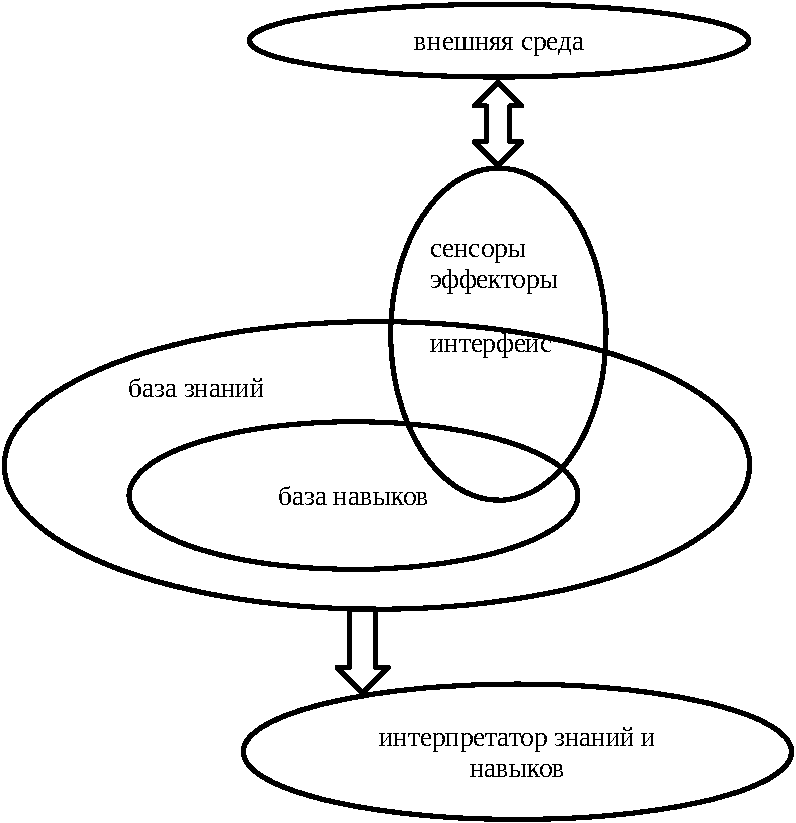
\includegraphics{Contents/part_intro/images/arch.pdf}}
		\bigskip
	\end{scnsubstruct}
\end{SCn}
\scnsourcecomment{Завершили Раздел \scnqqi{Предметная область и онтология интеллектуальных компьютерных систем нового поколения}}


\scsubsection[
    \protect\scneditor{Банцевич К.А.}
    \protect\scnmonographychapter{Глава 1.2. Интеллектуальные компьютерные системы нового поколения и технология комплексной поддержки их жизненного цикла}
    ]{Предметная область и онтология смыслового представления информации}
\label{sd_sem_inf_rep}
\begin{SCn}
	\scnsectionheader{Предметная область и онтология смыслового представления информации}

	\begin{scnsubstruct}

		\scnrelto{частная предметная область и онтология}{Предметная область и
			онтология информационных конструкций}
		\begin{scnhaselementrolelist}{класс объектов исследования}
			\scnitem{смысловое представление информации}
			\begin{scnindent}
				\scnidtf{смысл}
			\end{scnindent}
		\end{scnhaselementrolelist}

		\begin{scnhaselementrolelist}{класс объектов исследования}
			\scnitem{семантическая сеть}
				\begin{scnindent}
					\begin{scnsubdividing}
						\scnitem{нерафинированная семантическая сеть}
						\scnitem{рафинированная семантическая сеть}
					\end{scnsubdividing}
					\begin{scnsubdividing}
						\scnitem{абстрактная семантическая сеть}
							\begin{scnindent}
								\scnidtf{семантическая сеть, абстрагирующаяся от того, как
									физически представлены ее элементарные (атомарные) фрагменты, а также связи
									инцидентности между этими фрагментами}
							\end{scnindent}
						\scnitem{графически представленная семантическая сеть}
							\begin{scnindent}
								\scnidtf{нарисованная семантическая сеть}
							\end{scnindent}
						\scnitem{семантическая сеть, хранимая в графодинамической памяти}
							\begin{scnindent}
								\scnrelboth{следует отличать}{представление семантической сети
									в адресной памяти}
								\begin{scnindent}
									\scnnotsubset{семантическая сеть}
									\scnidtf{представление семантической сети в виде линейной
										информационной конструкции, которая хранится в адресной памяти и которая,
										строго говоря, уже не является семантической сетью, но является информационной
										конструкцией, семантически эквивалентной соответствующей (представляемой)
										семантической сети}
								\end{scnindent}
							\end{scnindent}
					\end{scnsubdividing}
				\end{scnindent}
			\scnitem{граф знаний}
			\begin{scnindent}
				\scnidtf{представление сложноструктурированного знания в виде графовой структуры}
			\end{scnindent}
			\scnitem{язык семантических сетей}
				\begin{scnindent}
					\scnidtf{язык, все тексты которого являются семантическими
						сетями}
					\begin{scnsubdividing}
						\scnitem{специализированный язык семантических сетей}
						\scnitem{универсальный язык семантических сетей}
					\end{scnsubdividing}
					\scnsuperset{язык рафинированных семантических сетей}
				\end{scnindent}
		\end{scnhaselementrolelist}

		\begin{scnrelfromvector}{рассматриваемые вопросы}
			\scnfileitem{Что такое семантические сети и в чем их принципиальное
				отличие от других вариантов представления информации}
			\scnfileitem{До какой степени можно минимизировать алфавит элементов
				семантических сетей}
			\scnfileitem{Можно ли все описываемые связи свести к бинарным связям и
				почему это целесообразно}
			\scnfileitem{Можно ли разработать \uline{универсальный} язык
				семантических сетей}
			\scnfileitem{До какой степени можно упростить синтаксические структуры
				семантических сетей до, условно говоря, рафинированного вида}
			\scnfileitem{Какими достоинствами обладает семантические сети}
		\end{scnrelfromvector}

		\begin{scnrelfromlist}{ссылка}
			\scnitem{Понятие Технологии OSTIS}
				\begin{scnindent}
					\scntext{аннотация}{В указанном сегменте \textit{Стандарта
							OSTIS} рассматриваются принципы, лежащие в основе \textit{Технологии OSTIS},
						основным из которых является ориентация на использование
						\textit{\uline{универсального} языка рафинированных семантических сетей} в
						качестве внутреннего языка \textit{интеллектуальных компьютерных систем}}
				\end{scnindent}
			\scnitem{Описание внутреннего языка ostis-систем}
				\begin{scnindent}
					\scntext{аннотация}{В указанном разделе \textit{Стандарта
						OSTIS} рассматриваются принципы, лежащие в основе \textit{универсального языка
						рафинированных семантических сетей}, используемого в качестве внутреннего языка
						\textit{ostis-систем} --- \textit{интеллектуальных компьютерных систем}
						следующего поколения}
				\end{scnindent}
			\scnitem{Описание языка графического представления знаний ostis-систем}
				\begin{scnindent}
					\scntext{аннотация}{В указанном разделе \textit{Стандарта
						OSTIS} рассматриваются принципы, лежащие в основе универсального языка
						графически представленных семантических сетей, используемого в
						\textit{пользовательском интерфейсе ostis-систем}}
				\end{scnindent}
			\scnitem{\scncite{Birukov1960}}
			\scnitem{\scncite{Morris2001}}
			\scnitem{\scncite{Pirs2009}}
			\scnitem{\scncite{Stepanov1971}}
			\scnitem{\scncite{MelchukST}}
		\end{scnrelfromlist}

		\bigskip
		\scnheader{знак}
		\scnidtf{фрагмент информационной конструкции, обладающий свойством,
			\uline{обозначать} некоторую сущность (объект), которая наряду с другими
			сущностями описывается указанной информационной конструкцией}
		\scntext{примечание}{\uline{Форма} представления знаков в известной степени
			условна и является результатом соглашения между носителями соответствующего
			языка. Знак может быть, например, представлен:
			\begin{scnitemize}
				\item  в виде фрагмента речевого сообщения (последовательностью
				фонем);
				\item в виде строки символов (последовательности букв) в
				заданном алфавите;
				\item в виде иероглифа, пиктограммы;
				\item в виде жеста.
			\end{scnitemize}}
		\scniselementrole{ключевой знак}{Предметная область и онтология информационных конструкций}
			\begin{scnindent}
				\scnhaselement{раздел Базы знаний Метасистемы OSTIS}
			\end{scnindent}
		\scntext{характеристика элементов данного множества}{Знаки,
			используемые в различных языках, характеризуются:
			\begin{scnitemize}
				\item синтаксической структурой, по совпадению (изоморфизму)
				которых для разных знаокв предполагается их синонимия;
				\item денотационной семантикой, т.е. той сущностью, которая
				обозначается соответствующим знаком;
				\item типом (классом) обозначаемой сущности, которая может
				быть:
				\begin{scnitemizeii}
					\item материальным(физическим) элементом (точкой)
					абстрактного пространства, множеством, которое может быть:
					\begin{scnitemizeiii}
						\item связью;
						\item классом;
						\item структурой;
					\end{scnitemizeiii}
					\item реальной и вымышленной сущностью;
					\item константной (конкретной) и переменной
					(произвольной) сущностью;
					\item постоянно существующей и временно существующей
					сущностью (прошлой, настоящей, будущей);
				\end{scnitemizeii}
				\item множеством тех связей, которые связывают сущность,
				обозначаемую данным знаком с другими сущностями, а также, если данный знак
				обозначает некоторую связь, множеством сущностей, которые связаны этой связью,
				т.е. сущностей, являющихся компонентом этой связи;
				\item текущим статусом самого знака в памяти кибернетической
				системы, который может быть:
				\begin{scnitemizeii}
					\item логически удаленным знаком;
					\item настоящим знаком;
					\item предлагаемым (возможно, будущим) знаком.
				\end{scnitemizeii}
			\end{scnitemize}}

		\bigskip
		\scnheader{денотат*}
		\scnidtf{денотат заданного знака*}
		\scnidtf{объект, обозначаемый заданным знаком*}
		\scnidtf{денотационная семантика заданного знака*}
		\scnidtf{смысл заданного знака*}
		\scnidtf{Бинарное ориентированное отношение, каждая пара которого
			связывает:
			\begin{scnitemize}
				\item некоторый знак, представленный в той или иной форме в тексте
				исследуемого языка;
				\item \uline{со знаком} той сущности, которая обозначается указанным
				выше знаком в рамках используемого метаязыка.
			\end{scnitemize}}

		\scntext{примечание}{Данное отношение используется, когда с помощью одного
			языка необходимо описать денотационную семантику другого языка. Фактически речь
			идет о переводе заданного знака, входящего в состав некоторого рассматриваемого
			текста, принадлежащего некоторому исследуемому языку (языку-объекту), на
			некоторый метаязык (в нашем случае на SC-код), денотационная семантика которого
			нам считается априори известной. Указанный перевод есть связь заданного знака с
			синонимичным ему знаком, входящим в состав текста, принадлежащего указанному
			метаязыку.}
		\scnrelboth{обратное отношение}{внешний sc-идентификатор*}
			\begin{scnindent}
				\scnidtf{быть знаком, обозначающим заданную сущность*}
			\end{scnindent}

		\scnheader{информационная конструкция}
		\scnidtf{информация}
		\scntext{примечание}{В общем случае информационная конструкция представляет
			собой сложную иерархическую структуру, каждому уровню иерархии которой
			соответствует определенный класс информационных конструкций.}
		\scnsuperset{синтаксически элементарный фрагмент информационной конструкции}
			\begin{scnindent}
				\scnidtf{атомарный фрагмент информационной конструкции}
				\scnidtf{элемент информационной конструкции}
				\scntext{примечание}{Примерами таких элементарных фрагментов информационных
					конструкций являются буквы}
				\scnsuperset{буква}
			\end{scnindent}
		\scnsuperset{простой знак}
			\begin{scnindent}
				\scnidtf{семантически элементарный фрагмент информационной конструкции}
				\scnsubset{знак}
			\end{scnindent}
		\scnsuperset{выражение}
			\begin{scnindent}
				\scnidtf{сложный (непростой) знак}
				\scnidtf{знак, являющийся одновременно некоторым знанием обозначаемой
					сущности (спецификацией этой сущности)}
				\scnidtf{знак, построенный как выражение вида тот, который... }
				\scnidtf{знак, в состав которого входят другие знаки}
				\scnsubset{знак}
			\end{scnindent}
		\scnsuperset{простой текст}
			\begin{scnindent}
				\scnidtf{минимальная синтаксически целостная и корректная (правильная)
					информационная конструкция, включающая в себя:
					\begin{scnitemize}
						\item знак некоторой описываемой связи;
						\item минимальную спецификацию указанного знака связи (указание
						отношения, которому это связь принадлежит);
						\item указание \uline{всех} компонентов описываемой связи (знаков всех
						сущностей, связываемых этой связью, и/или всех знаков, связываемых этой связью
						-- описываемая связь может связывать не только внешние	описываемые сущности,
						но и сами знаки);
						\item если описываемая связь не является бинарной, то связи с её
						компонентами могут потребовать явного представления знаков этих связей с
						дополнительным указанием роли этих компонентов.
					\end{scnitemize}}
				\scnsubset{текст}
			\end{scnindent}
		\scnsuperset{сложный текст}
			\begin{scnindent}
				\scnidtf{информационная конструкция, являющаяся результатом соединения
					нескольких простых текстов}
				\scnsubset{текст}
			\end{scnindent}
		\scnsuperset{простое знание}
			\begin{scnindent}
				\scnidtf{минимальная семантические целостная информационная конструкция}
				\scnidtf{знание, в состав которого не входят другие знания}
				\scnsubset{знание}
			\end{scnindent}
		\scnsuperset{сложное знание}
			\begin{scnindent}
				\scnidtf{информационная конструкция, являющаяся результатом соединения
					нескольких простых знаний}
				\scnidtf{знание, в состав которого не входят другие знания}
				\scnsubset{знание}
			\end{scnindent}
		\scniselementrole{ключевой знак}{Предметная область и онтология информационных конструкций}

		\scnheader{стандартизация моделей представления и обработки информации}
		\scnidtf{предлагаемый подход к решению проблем, препятствующих дальнейшей эволюции компьютерных систем и технологий}
		\scntext{примечание}{Анализ проблем эволюции компьютерных систем разного уровня сложности, разного уровня обучаемости и
		интеллектуальности, разного назначения показывает, что проклятие \scnqq{вавилонского столпотворения} и, как следствие,
		несовместимость, дублирование и субъективизм согласовываемых информационных ресурсов и моделей их обработки 
		нас преследует везде:
		\begin{scnitemize}
			\item и в развитии традиционных компьютерных систем;
			\item и в развитии технологий искусственного интеллекта;
			\item и в развитии методов и средств информатизации научной и инженерной деятельности.
		\end{scnitemize}}
		

		\scnheader{проблема обеспечения совместимости информационных ресурсов и моделей их обработки}
		\begin{scnrelfromlist}{аспекты решения}
			\scnitem{обеспечение совместимости между различными компонентами компьютерных систем, а также между
			целостными компьютерными системами, входящими в коллективы компьютерных систем}
			\scnitem{обеспечение совместимости, то есть высокого уровня взаимопонимания между различными компьютерными 
			системами и их пользователями}
			\scnitem{беспечение междисциплинарной совместимости, то есть конвергенции различных областей знаний}
			\scnitem{методы и средства постоянного мониторинга и восстановления совместимости в условиях интенсивной
			эволюции компьютерных систем и их пользователей, которая часто нарушает достигнутую совместимость
			(согласованность) и требует дополнительных усилий на ее восстановление}
		\end{scnrelfromlist}

		\scnheader{подход к решению проблем эволюции компьютерных систем}
		\scntext{примечание}{Суть предлагаемого нами подхода к решению проблем эволюции компьютерных систем заключается:
		\begin{scnitemize}
			\item в объединении всех указанных выше направлений эволюции компьютерных систем (как общих направлений, так
				и частных)
			\item в трактовке проблемы обеспечения \textbf{совместимости} различных видов знаний, различных
				моделей решения задач, различных компьютерных систем как \textbf{ключевой проблемы} эволюции компьютерных
				систем, решение которой существенно упростит решение и многих других проблем
		\end{scnitemize}}

		\scnheader{совместимость}
		\scntext{примечание}{Без обеспечения совместимости информационных ресурсов, используемых в разных компьютерных
		системах, а также информационных ресурсов, представляющих знания различного семантического вида невозможно:
		\begin{scnitemize}
			\item ни создавать \textbf{коллективы компьютерных систем}, способные координировать свои действия при кооперативном
				расширении сложных задач;
			\item ни создавать \textbf{гибридные компьютерные системы}, которые способны при решении сложных комплексных
				задач использовать всевозможные сочетания разных видов знаний и разных моделей решения задач;
			\item ни использовать \textbf{компонентную методику проектирования} компьютерных систем \textbf{на всех уровнях} иерархии
				проектируемых систем.
		\end{scnitemize}
		О какой информационной совместимости и взаимопонимании (в том числе между специалистами) можно говорить
		при наличии ужасающей понятийной и терминологической неряшливости, терминологического псевдотворчества,
		в том числе, в области информатики.}
		
		\scnheader{следует отличать*}
		\begin{scnhaselementset}
			\scnfileitem{совместимость как один из факторов обучаемости, как \textbf{способность} к быстрому повышению уровня
				согласованности (интеграции, взаимопонимания). Сравните обучаемость как \textbf{способность} к быстрому расширению
				знаний и навыков, но никак не характеристика объема и качества приобретенных знаний и навыков}
			\scnfileitem{совместимость как характеристика достигнутого уровня согласованности (интеграции, взаимопонимания)}
		\end{scnhaselementset}

		\scnheader{следует отличать*}
		\begin{scnhaselementset}
			\scnfileitem{интеллект компьютерной системы как \textbf{уровень} (объем и качество) приобретенных знаний и навыков}
			\scnfileitem{интеллект компьютерной системы как \textbf{способность} к быстрому расширению и
				совершенствованию знаний и навыков, то есть как \textbf{скорость} повышения уровня знаний и навыков}
		\end{scnhaselementset}

		\scnheader{следует говорить*}
		\begin{scnhaselementset}
			\scnfileitem{о \textbf{способности} к быстрому повышению уровня согласованности}
			\scnfileitem{о достигнутом уровне согласованности}
			\scnfileitem{о самом \textbf{процессе} повышения уровня согласованности}
			\scnfileitem{о перманентном процессе восстановления (поддержки, сохранения) достигнутого уровня согласованности,
				поскольку в ходе эволюции компьютерных систем и их пользователей (то есть в ходе расширения и повышения
				качества их знаний и навыков) уровень их согласованности может понижаться}
		\end{scnhaselementset}

		\scnheader{совместимость различных видов знаний, различных моделей решения задач и различных компьютерных систем}
		\begin{scnrelfromlist}{главный фактор}
			\scnitem{унификация представления информации в памяти компьютерных систем}
				\begin{scnindent}
					\scnidtf{стандартизация представления информации в памяти компьютерных систем}
				\end{scnindent}
			\scnitem{унификация принципов организации обработки информации в памяти компьютерных систем}
		\end{scnrelfromlist}

		\scnheader{унификация представления информации в памяти компьютерных систем}
		\begin{scnrelfromset}{предполагает}
			\scnitem{синтаксическая унификация используемой информации}
			\begin{scnindent}
				\scnidtf{унификация формы представления (кодирования) этой информации}
			\end{scnindent}
			\scnitem{семантическая унификация используемой информации}
			\begin{scnindent}
				\scnidtf{согласование и точная спецификация всех (!) используемых понятий 
					(концептов) с помощью иерархической системы формальных онтологий}
			\end{scnindent}
		\end{scnrelfromset}
		\scntext{примечание}{Важно отметить, что грамотная унификация (стандартизация) должна не ограничивать творческую свободу 
		разработчика, а гарантировать \textbf{совместимость} его результатов с результатами других разработчиков.}

		\scnheader{следует отличать*}
		\begin{scnhaselementset}
			\scnitem{внутреннее представление информации}
			\begin{scnindent}
				\scnidtf{кодирование информации в памяти компьютерной системы}
			\end{scnindent}
			\scnitem{внешнее представление информации}
			\begin{scnindent}
				\scnidtf{обеспечение однозначности интерпретации (понимания, трактовки) этой информации
					разными пользователями и разными компьютерными системами}
			\end{scnindent}
		\end{scnhaselementset}

		\scnheader{стандарт}
		\scntext{примечание}{Подчеркнем, что текущая версия любого \textbf{стандарта} --- это не догма, а только опора для дальнейшего его совершенствования.}
		\begin{scnrelfromlist}{цель}
			\scnitem{обеспечение совместимости технических решений}
			\scnitem{минимализация дублирования (повторения) решений}
		\end{scnrelfromlist}
		\scntext{критерий качества}{ничего лишнего}

		\bigskip\scnheader{смысловое представление информации}
		\scnidtf{смысловая форма представления информации}
		\scnidtf{смысловое представление информационной конструкции}
		\scnidtf{знаковая конструкция (текст), представленная в смысловой
			форме}
		\scnidtf{запись (представление) информационной конструкции на смысловом уровне}
		\scnidtf{информационная конструкция, синтаксическая структура которой близка ее смыслу, то есть близка 
			описываемой конфигурации связей между описываемыми сущностями}
		\scnidtftext{часто используемый sc-идентификатор}{смысл}
		\scnidtf{смысловое представление}
		\scnidtf{семантическое представление информации}
		\scntext{основной принцип}{Как можно меньше лишнего, не имеющего
			отношения к смыслу представляемой информации.}
		\scnidtf{такое представление информационной конструкции, которое
			существенно упрощает соответствие между структурой самой этой информационной
			конструкции и описываемой (отображаемой) ею конфигурацией связей между
			рассматриваемыми (исследуемыми) сущностями}
		\scnidtf{смысловое представление знаковой конструкции}
		\scnidtf{абстрактная знаковая конструкция, являющаяся
			\uline{инвариантом} соответствующего максимального класса семантически
			эквивалентных знаковых конструкций}
		\scnidtf{смысл информационной конструкции}
		\scnidtf{денотационная семантика информационной конструкции}
		\scntext{примечание}{Суть (смысл, денотационная семантика) любой
			информационной конструкции (информационной модели) сводится к описанию системы
			(конфигурации) связей между списываемыми (рассматриваемыми) сущностями. Важно,
			чтобы эта суть не была \uline{закамуфлирована} различными синтаксическими
			деталями, не имеющими никакого отношения к указанному смыслу (синтаксическая
			структура знаков, многократное повторение одного и того же знака, синонимия,
			омонимия, местоимения, предлоги, знаки препинания, разделители, ограничители,
			падежи и т.п.) а обусловленными \uline{формой} представления информационных
			конструкций, например, их линейностью.}
		\scntext{пояснение}{Смысловое представление любой информации в
			конечном счете сводится:
			\begin{scnitemize}
				\item к перечню знаков конкретных описываемых сущностей --- как первичных
				            сущностей, так и вторичных сущностей, которые сами являются информационными
				            конструкциями (фрагментами данной конструкции);
				\item к явному описанию связи между знаками вторичных сущностей и
				            самими этими сущностями (т.е. фрагментами информационной конструкции);
				\item к описанию других связей между описываемыми сущностями
			\end{scnitemize}
			\vspace{-0.6\baselineskip}}
		\scntext{пояснение}{Формализация смысла представляемой информации,
			т.е. строгое уточнение того, что такое \textit{смысловое представление
				информации}, является объективной основой для \uline{унификации} представления
			информации в \textit{памяти компьютерных систем} и \uline{ключом} к решению
			многих проблем семантической совместимости и эволюции компьютерных систем и
			технологий.
			
			Согласно \textit{Мартынову В. В.}, <<фактически
			всякая мыслительная деятельность человека (не только научная), как полагают
			многие ученые, использует \uline{внутренний семантический код}, на который
			переводят с естественного языка и с которого переводят на естественный язык.
			Поразительная способность человека к идентификации огромного множества
			структурно различных фраз с одинаковым \textit{смыслом} и способность
			\uline{запомнить смысл вне этих фраз} убеждает нас в этом.>>
			
			Приведем также слова \textit{Мельчука И. А.}:
			
			<<Идея была следующая --- язык надо описывать следующим образом: надо уметь записывать смыслы фраз. \uline{Не
			фразы, а их \textit{смыслы}}, что отдельно. Плюс построить систему, которая по
			смыслу строит фразу. Это та область или тот поворот исследований, при котором
			интуиция способного лингвиста работает лучше всего: как выразить на данном
			языке данный смысл. Это --- то, для чего лингвистов учат.
			
			Лингвистический	\textit{смысл} научного текста --- это совсем не то, что ты, читая его, из него
			извлекаешь. Это, очень грубо говоря, инвариант синонимических перифраз. Ты
			можешь один и тот же смысл выразить очень многими способами. Когда ты говоришь,
			то можешь сказать по-разному: \scnqqi{Сейчас я налью тебе вина}, или: \scnqqi{Дай, я тебе
			предложу вина}, или: \scnqqi{Не выпить ли нам по бокалу?}, --- все это имеет один и тот
			же смысл. И вот можно придумать, как записывать этот \textit{смысл}. Именно
			его. Не фразу, а \textit{смысл}. И работать надо от этого \textit{смысла} к
			реальным фразам. Синтаксис там по дороге тоже нужен, но он нужен именно по
			дороге, он не может быть ни конечной целью, ни начальной точкой. Это --
			промежуточное дело.>>.}
				\begin{scnindent}
					\begin{scnrelfromlist}{источник}
						\scnitem{\scncite{Melchuk}}
						\scnitem{\scncite{Martynov}}
					\end{scnrelfromlist}
				\end{scnindent}
		\scntext{примечание}{Грамотная унификация (стандартизация) \textit{смыслового
				представления информации} не должна привести к ограничению творческой свободы
			авторов различного вида публикуемых научно-технических знаний (и, в том числе,
			разработчиков \textit{баз знаний}), не должна гарантировать
			\textit{семантическую совместимость} различных \textit{знаний}, представленных
			различными авторами (разумеется, при условии соблюдения соответствующих правил
			построения этих \textit{знаний}). При этом любые \textit{стандарты} (в том
			числе и принятые стандарты \textit{смыслового представления информации}) должны
			постоянно эволюционировать. Текущая версия любого стандарта должна быть не
			догмой, а точкой опоры для дальнейшего совершенствования этого стандарта.}
		\scnsuperset{УСК}
			\begin{scnindent}
				\scnidtf{Универсальный Семантический Код}
				\scnrelfrom{автор}{Мартынов В. В.}
				\scntext{примечание}{Разработанный Мартыновым В. В. Универсальный
					Семантический Код стал важнейшим этапом создания универсальных формальных
					средств смыслового представления знаний. Основная методологическая идея
					\textit{Мартынова В. В.}, касающаяся построения \textit{языка смыслового
					представления знаний}, заключается в том, чтобы выделить смысловые кирпичики ,
					имеющие достаточно общий характер, а многообразие конкретных смыслов
					конструировать комбинаторно за счёт различных комбинаций (конфигураций) из этих
					кирпичей. Это можно назвать принципом минимизации типов атомарных смысловых
					фрагментов.}
				\scnrelto{ключевой знак}{\scncite{Martynov1984}}
			\end{scnindent}
		\scnsuperset{семантическая сеть}
			\begin{scnindent}
				\scnsuperset{рафинированная семантическая сеть}	
			\end{scnindent}
		\scntext{примечание}{Уточнение принципов \textbf{смыслового представления информации} основано, во-первых, на четком
			противопоставление \textbf{внутреннего языка компьютерной системы}, используемого для хранения информации в памяти
			компьютера, и \textbf{внешних языков компьютерной системы}, используемых для общения (обмена сообщениями) компьютерной
			системы с пользователями и другими компьютерными системами (смысловое представление используется
			исключительно для \textbf{внутреннего представления} информации в памяти компьютерной системы), и, во-вторых,
			на максимально возможном упрощении синтаксиса внутреннего языка компьютерной системы при обеспечении
			универсальности путем исключения из такого внутреннего универсального языка средств, обеспечивающих
			коммуникационную функцию языка (то есть обмен сообщениями). Так, например, для внутреннего языка компьютерной 
			системы излишними являются такие коммуникационные средства языка, как союзы, предлоги, разделители, ограничители, 
			склонения, спряжения и другие. Внешние языки компьютерной системы могут быть как близки ее внутреннему языку, так и 
			весьма далеки от него (как, например, естественные языки)}

		\scnheader{смысловое представление информации*}
		\scnidtftext{пояснение}{\textit{Бинарное ориентированное отношение},
			каждая \textit{пара} которого связывает некоторую \textit{информационную
				конструкцию} со смысловым представлением этой \textit{информационной
				конструкции*}.}
		\scnsubset{формализация*}
		\bigskip
		
		\scnheader{смысл}
		\scnidtf{\textbf{абстрактная} знаковая конструкция, принадлежащая внутреннему языку компьютерной системы,
			являющаяся \textbf{инвариантом} максимального класса семантически эквивалентных знаковых конструкций (текстов),
			принадлежащих самым разным языкам}
			\begin{scnrelfromlist}{требования}
				\scnitem{\textbf{универсальность}}
					\begin{scnindent}
						\scnidtf{возможность представления любой информации}
					\end{scnindent}
				\scnitem{\textbf{отсутствие синонимии знаков}}
					\begin{scnindent}
						\scnidtf{многократного вхождения знаков с одинаковыми денотатами}
					\end{scnindent}
				\scnitem{\textbf{отсутствие дублирования информации} в виде семантически эквивалентных текстов}
					\begin{scnindent}
						\scntext{примечание}{не путать с логической	эквивалентностью}
					\end{scnindent}
				\scnitem{\textbf{отсутствие омонимичных знаков}}
					\begin{scnindent}
						\scntext{примечание}{в том числе местоимений}
					\end{scnindent}
				\scnitem{\textbf{отсутствие у знаков внутренней структуры}}
					\begin{scnindent}
						\scntext{примечание}{атомарный характер знаков}
					\end{scnindent}
				\scnitem{\textbf{отсутствие склонений, спряжений}}
					\begin{scnindent}
						\scntext{следствие}{отсутствия у знаков внутренней структуры}
					\end{scnindent}
				\scnitem{\textbf{отсутствие фрагментов} знаковой конструкции, не являющихся знаками}
					\begin{scnindent}
						\scntext{пример}{разделители, ограничители и так далее}
					\end{scnindent}
				\scnitem{\textbf{выделение знаков связей}, компонентами которых могут быть любые знаки, с которыми знаки связей
				связываются синтаксически задаваемыми отношениями инцидентности.}
			\end{scnrelfromlist}

		\scnheader{принципы смыслового представления информации в памяти компьютерной системы}
		\scntext{следствие}{Знаки сущностей, входящие в смысловое представление информации, \textbf{не являются именами}
			(терминами) и, следовательно, не привязаны ни к какому естественному языку и не зависят от субъективных
			терминотворческих пристрастий различных авторов. Это значит, что при коллективной разработке смыслового
			представления каких-либо информационных ресурсов терминологические споры исключены.}
		\scntext{следствие}{Эти принципы приводят к нелинейным знаковым конструкциям (к графовым структурам), что усложняет реализацию памяти
			компьютерных систем, но существенно упрощает ее логическую организацию (в частности, ассоциативный доступ).}

		\scnheader{нелинейность смыслового представления информации}
		\begin{scnrelfromlist}{обусловлено}
			\scnfileitem{Каждая описываемая сущность, то есть сущность, имеющая соответствующий ей знак, может иметь неограниченное
				число связей с другими описываемыми сущностями;}
			\scnfileitem{каждая описываемая сущность в смысловом представлении имеет единственный знак, так как синонимия
				знаков здесь запрещена;}
			\scnfileitem{все связи между описываемыми сущностями описываются (отражаются, моделируются) связями между знаками
				этих описываемых сущностей.}
		\end{scnrelfromlist}

		\scnheader{универсальное смысловое представления информации}
		\scntext{примечание}{Суть можно сформулировать в виде следующих положений:
		\begin{scnitemize}
			\item Смысловая знаковая конструкция трактуется как множество знаков, взаимно-однозначно обозначающих различные
				сущности (денотаты этих знаков) и множество связей между этими знаками;
			\item Каждая связь между знаками трактуется, с одной стороны, как множество знаков, связываемых этой связью,
				а, с другой стороны, как описание (отражение, модель) соответствующей связи, которая связывает денотаты
				указанных знаков или денотаты одних знаков непосредственно с другими знаками, или сами эти знаки. Примером
				первого вида связи между знаками является связь между знаками материальных сущностей, одна из
				которых является частью другой. Примером второго вида связи между знаками является связь между знаком
				множества знаков и одним из знаком, принадлежащих этому множеству, а также связь между знаком и знаком
				файла, являющегося электронным отражением структуры представления указанного знака во внешних знаковых
				конструкциях. Примерами третьего вида связи между знаками является связь между синонимичными знаками;
			\item Денотатами знаков могут быть (1) не только конкретные (константные, фиксированные), но и произвольные
				(переменные, нефиксированные) сущности, \scnqq{пробегающие} различные множества знаков (возможных значений),
				(2) не только реальные (материальные), но и абстрактные сущности (например, числа, точки различных
				абстрактных пространств), (3) не только \scnqq{внешние}, но и \scnqq{внутренние} сущности, являющиеся множествами
				знаков, входящих в состав той же самой знаковой конструкции.
		\end{scnitemize}}
			
		\scnheader{формализация*}
		\scniselement{бинарное ориентированное отношение}
		\scnidtf{формализация информации*}
		\scnidtf{пара, связывающая менее формализованное и более
			формализованное представление некоторой информации*}
		\scnidtf{формализация информационной модели некоторой описываемой
			(моделируемой) системы взаимосвязанных сущностей*}
		\scnidtf{Бинарное ориентированное отношение, каждая \textit{пара}
			которого, связывает два \textit{семантически эквивалентных} знания, второе из
			которых является более точным (более точно сформированным) знанием по сравнению
			с первым \textit{знанием}*.}
		\scntext{пояснение}{Повышение точности (строгости) формулировки
			знания --- минимизация (а в идеале --- исключение) \uline{неоднозначной}
			семантической интерпретации этой формулировки, т.е. несоответствия того, что
			хотел сказать  автор формулировки, и того, как его поняли. Формализация знаний
			предполагает (1) точное (строгое) описание \textit{синтаксиса и денотационной
				семантики} того \textit{языка}, на котором формулируются \textit{знания} и (2)
			максимально возможное \uline{упрощение} синтаксических и семантических
			принципов, лежащих в основе указанного \textit{языка}. Очевидно, что
			\textit{естественные языки} указанным требованиям не удовлетворяют и,
			следовательно, не могут быть основой для точной формулировки
			\textit{научно-технических знаний} и, соответственно, для представления этих
			\textit{знаний} в \textit{памяти интеллектуальных компьютерных систем}.
			Очевидно также, что разработка \textit{\uline{универсального} языка}
			формального представления научно-технических знаний является \uline{основой}
			для глубокой конвергенции различных научно-технических дисциплин, для
			расширения областей применения современной математики и даже для появления
			новых разделов математики, которые, например, изучают общие свойства
			\textit{универсального смыслового пространства} и, в частности, свойство
			семантического расстояния(семантической близости) как между различными
			\textit{знаками}, так и между различными \textit{знаковыми конструкциями}
			(конфигурациями знаков).}
			\begin{scnindent}
				\scntext{примечание}{Слово математика  означает точное знание .}
					\begin{scnindent}
						\scnrelto{цитата}{\scncite{Arnold2012}}
					\end{scnindent}
			\end{scnindent}
		\scntext{примечание}{Формализация информационной модели есть не что иное как
			движение  в сторону семантического (смыслового) представления этой модель, т.е.
			переход к такому представлению этой модели, в котором мы избавляемся от всего,
			не имеющего отношения к сути моделируемой системы и касающегося только способа
			построения этой модели (т.е. её синтаксической структуры). }
		\scntext{примечание}{Нет проблемы записать любое \textit{знание} в
			компьютерную \textit{память}. Для этого надо придумать соответствующий формат
			их кодирования. Но есть проблема представить это \textit{знание} так, чтобы с
			ним было легко работать, чтобы с использованием этого \textit{знания} можно
			было достаточно удобно (без лишних накладных расходов, обусловленных выбранным
			способом представления) решать самые различные информационные \textit{задачи}
			(задачи интеграции знаний, информационного поиска по базе знаний, верификации и
			оптимизации баз знаний, логического вывода, поиска способов решения задач,
			хранимых в базе знаний и т. д.).Какими характеристиками должно обладать удобное
			представление знаний, удовлетворяющее указанным требованиям. Очевидно, что
			такое представление есть не что иное, как формальная (математическая) модель,
			семантически эквивалентная этим знаниям. Т.е. удобно представить знание --- это
			фактически построить соответствующую этому знанию \textit{математическую
				модель}.Для интеллектуальных компьютерных систем важно не просто приобрести
			знания, но и представить их в такой форме, которая была бы удобна не только для
			человека (пользователя и разработчика), но и для различных компьютерных систем,
			т.е. не требовала бы переоформление (перезаписи) этих знаний для различных
			компьютерных систем. Очевидно, что такая форма записи (представления) знаний
			должна быть абсолютно не зависящий от различных компьютерных платформ.Это и
			есть главная цель формализации знаний, обеспечивающей эффективную автоматизацию
			обработки этих знаний.}

		\scnheader{формальное представление информации}
		\scnsubset{информация}
			\begin{scnindent}
				\scnidtf{информационная конструкция}
			\end{scnindent}
		\scntext{вопрос}{Почему разработка и использование формальных моделей
			(математических моделей) представления \textit{информации} является важнейшим
			этапом развития любой научной и научно-технической дисциплины.}
		\begin{scnindent}
			\begin{scnrelfromset}{ответ}
				\scnfileitem{Формализация любой \textit{предметной области} даёт
					возможность более конструктивно накапливать, интегрировать, понимать и
					систематизировать новые \textit{знания} об этой \textit{предметной области}}
				\scnfileitem{Формализация \textit{предметной области} обеспечивает
					более строгую верификацию, обоснование (аргументацию, доказательство) и
					согласование различных точек зрения}
				\scnfileitem{Формализация \textit{предметной области} создает условия
					для разработки строгих и легко воспроизводимых (реализуемых) \textit{методов}
					решения различных \textit{классов задач}}
			\end{scnrelfromset}
		\end{scnindent}
		\scnrelto{достоинства}{формальное представление информации}
		\scnidtf{формальное (формализованное) представление информационной
			конструкции}
		\scnsubset{смысловое представления информации}
		\scntext{примечание}{Высшим уровнем качества \textit{формального
				представления информации} является смысловое представление этой информации}
		\scnidtf{формальная модель системы описываемых взаимосвязанных
			сущностей}
		\scnidtf{математическая модель системы описываемых взаимосвязанных
			сущностей}
		\scnidtf{формула}
		\scntext{примечание}{Сам термин \scnqqi{\textit{формальное представление
				информации}} свидетельствует о том, что при таком представлении
			\textit{информации} сама \uline{форма} представляемой информационной
			конструкции (т.е. синтаксическая структура этой конструкции) имеет очевидную
			аналогию с описываемой конфигурацией связей между соответствующими
			соответствующими описываемыми \textit{сущностями}.В предельном идеальном
			случае указанная аналогия между формой и смыслом информационной конструкции
			должна быть изоморфизмом.}
		\scntext{примечание}{Формализация формализации рознь и, соответственно,
			степень приближения формы представления информации к идеальному  смысловому
			представлению может быть различной. Разработка такого идеального  \textit{языка
				смыслового представления информации} должна руководствоваться следующими
			основными критериями:
			\begin{scnitemize}
				\item максимально возможное упрощения синтаксиса (как можно меньше
				синтаксических излишеств и синтаксического разнообразия);
				\item обеспечение \uline{универсальности} языка.
			\end{scnitemize}
			Подчеркнем, что обеспечение универсальности \textit{языка смыслового
				представления информации} является весьма нетривиальной задачей, т.к. сложно
			одновременно достигнуть две противоречащие друг другу цели- обеспечить простоту
			синтаксиса языка и его неограниченную семантическую мощность. Косвенным
			подтверждением этого является большое количество созданных человечеством
			специализированных \textit{формальных языков}, \textit{языков смыслового
				представления информации} и даже \textit{языков семантических сетей}, что
			свидетельствует о востребованности \textit{смыслового представления
				информации}.}
		\begin{scnsubdividing}
			\scnitem{формальное представление информации, не являющееся смысловым}
			\scnitem{смысловое представление информации, не являющееся
				семантической сетью}
			\scnitem{нерафинированная семантическая сеть}
				\begin{scnindent}
					\scnidtf{смысловое представления информации 2-го уровня}
				\end{scnindent}
			\scnitem{рафинированная семантическая сеть}
				\begin{scnindent}
					\scnidtf{смысловое представление информации 3-го уровня}
				\end{scnindent}
		\end{scnsubdividing}

		\bigskip
		\scnheader{язык смыслового представления информации}
		\begin{scnrelfromlist}{ключевое свойство}
			\scnitem{однозначность представления информации в памяти каждой компьютерной системы}
			\begin{scnindent}
				\scnidtf{отсутствие семантически эквивалентных знаковых	конструкций, принадлежащих 
					смысловому языку и хранимых в одной смысловой памяти}
				\scntext{примечание}{При этом логическая эквивалентность таких знаковых конструкций 
					допускается и используются, например, для компактного представления некоторых знаний,
					хранимых в смысловой памяти.}
			\end{scnindent}
		\end{scnrelfromlist}

		\scnheader{смысловое представление информации, не являющееся семантической сетью}
		\scntext{примечание}{Данному уровню смыслового представления информации
			соответствуют предлагаемые нами универсальные формальные языки SCs-код и SCn-код}
		\scnsuperset{SCs-код}
			\begin{scnindent}
				\scniselement{универсальный формальный язык}
				\scniselementrole{ключевой знак}{Описание языка линейного представления знаний ostis-систем}
			\end{scnindent}
		\scnsuperset{SCn-код}
		\begin{scnindent}
			\scniselement{универсальный формальный язык}
			\scniselementrole{ключевой знак}{Описание языка структурированного представления знаний ostis-систем}
		\end{scnindent}
		\begin{scnrelfromvector}{принципы, лежащие в основе}
			\scnfileitem{В состав \textit{смыслового представления информации, не
				являющегося семантической сетью} могут входить все уровни иерархии
				представления информационной конструкции --
				\begin{scnitemize}
					\item синтаксически элементарные фрагменты информационной конструкции,
					из которых строятся простые знаки описываемых сущностей, а также разделители и
					ограничители
					\item простые знаки
					\item выражения
					\item простые тексты
					\item сложные тексты
					\item простые знания
					\item сложные знания.
				\end{scnitemize}}

			\scnfileitem{Множество всех описываемых сущностей, \uline{не являющихся
					связями}, разбивается на два подмножества:
				\begin{scnitemize}
					\item каждой сущности, принадлежащей первому подмножеству,
					\uline{взаимно однозначно} соответствует множество \uline{синтаксически
						эквивалентных} (синтаксически одинаковых) \textit{простых знаков}, каждый из
					которых обозначает указанную сущность
					\item каждой сущности, принадлежащей второму подмножеству,
					соответствует в общем случае \uline{семейство} множеств, кажо из которых
					является максимальным множеством синтаксически эквивалентных выражений,
					обозначающих указанную сущность.
				\end{scnitemize}}
				\begin{scnindent}
					\scntext{следовательно}{Здесь синонимия \textit{простых знаков},
						имеющих \uline{разную} синтаксическую структуру, отсутствует, а вот синонимия
						\textit{выражений}, имеющих разную синтаксическую структуру, вполне возможна.
						Подчеркнем при этом, что в рамках \textit{смыслового представления информации,
							не являющегося семантической сетью},
						% \bigspace
						\textit{знаки} (как \textit{простые знаки}, так и \textit{выражения}),
						имеющие одинаковую синтаксическую структуру, считаются также и семантически
						эквивалентными, т.е. обозначающими одну и ту же сущность. Это означает
						отсутствие омонимии синтаксически эквивалентных знаков.}
					\scntext{следовательно}{В рамках \textit{смыслового представления
							информации, не являющегося семантической сетью}, простые знаки, обозначающие
						\uline{разные} сущности, имеют легко устанавливаемое отличие своих
						синтаксических структур, а простые знаки, обозначающие одну и ту же сущность
						имеют легко устанавливаемое сходство своих синтаксических структур. Таким
						образом, в рамках \textit{смыслового представления информации, не являющегося
							семантической сетью},
						% \bigspace
						\uline{дублирование знаков}, т.е. многократное вхождение
						\textit{знаков} одной и той же сущности, \uline{допускается}.}
				\end{scnindent}
			\scnfileitem{Связи как вид описываемых сущностей имеют очень важные
				особенности:
				\begin{scnitemize}
					\item каждой описываемой \textit{связи} \uline{однозначно}, а в
					подавляющем числе случаев и \uline{взаимно однозначно} соответствует
					\textit{простой текст}, являющийся контекстом (спецификацией) этой
					\textit{связи}
					\item весьма редки \textit{кратные связи}, т.е. \textit{свзяи},
					принадлежащие одному и тому же \textit{отношению} и связывающие одинаковым
					образом одни и те же \textit{сущности}
					\item довольно редко \textit{связи} являются компонентами других
					\textit{связей}.
				\end{scnitemize}}
				\begin{scnindent}
					\scntext{следовательно}{Для подавляющего числа описываемых
						\textit{связей} нет никакой необходимости вводить обозначающие их
						\textit{знаки}, если эти \textit{связи} описываются соответствующими
						\textit{простыми текстами}. Вместо таких \textit{знаков} можно ввести условные
						представления этих \textit{связей}, отражающие их вид и направленность. Такие
						условные представления (изображения) описываемых \textit{связей} можно считать
						\textit{знаками}, но \textit{знаками}, семантические свойства которых
						принципиально отличаются от тех \textit{знаков} описываемых \textit{сущностей},
						которые мы рассматривали выше. Любые данного вида разные \textit{знаки}
						описываемых \textit{связей} даже, если, они являются \textit{синтаксически
							эквивалентными}, т.е. имеют одинаковую структуру, считаются \textit{знаками}
						\uline{разных} описываемых \textit{связей}. Синонимия таких \textit{знаков}
						принципиально возможна, но только в том случае, если \textit{простые тексты},
						описывающие соответствующие \textit{связи}, будут полностью
						\uline{продублированы}.}
				\end{scnindent}
			\scnfileitem{Для описания связей между описываемыми сущностями в
				смысловом представлении информации нет необходимости использовать такие приемы
				естественных языков, как склонения, спряжения, семантическая значимость
				последовательности знаков.}
			\scnfileitem{В случае, если с помощью \textit{простых текстов}
				необходимо описать контекст (спецификацию) нескольких \uline{кратных}
				\textit{связей}, все эти \textit{связи} необходимо обозначить \textit{знаками}
				первого типа --- знаками, \textit{синтаксическая структура} каждого из которых
				\uline{уникальна.}Кроме этого, необходимо ввести знак, который обозначает
				\textit{связь инцидентности} между описываемой \textit{связью} и компонентом
				этой \textit{связи}, и который относится к числу \textit{знаков} второго типа
				-- \textit{знаков}, разные экземпляры (разные вхождения) которого считаются
				обозначениями \uline{разных} \textit{связей}}
			\scnfileitem{Для явного указания синонимии двух разных \textit{знаков}
				первого типа, имеющих разную \textit{синтаксическую структуру}, вводится
				фиктивная \textit{связь равенства}, которая сама не является описываемой
				\textit{связью}, а только указывает факт синонимии двух \textit{знаков}, по
				крайней мере один из которых должен быть \textit{выражением}.}
			\scnfileitem{Каждая описываемая \textit{сущность} должна быть
				специфицирована путем указания типа этой \textit{сущности}. Описываемая
				\textit{сущность} может быть:
				\begin{scnitemize}
					\item \textit{материальной сущностью}
					\item \textit{точкой абстрактного пространства}
					\item \textit{множеством}:
						\begin{scnitemizeii}
							\item \textit{связью}
							\item \textit{классом}
							\item \textit{структурой}
						\end{scnitemizeii}
					\item \textit{реальной сущностью}
					\item \textit{вымышленной сущностью}
					\item \textit{константой}
					\item \textit{переменной}
					\item \textit{постоянной сущностью}
					\item \textit{временной сущностью}:
						\begin{scnitemizeii}
							\item \textit{прошлой сущностью}
							\item \textit{настоящей сущностью}
							\item \textit{будующей сущностью}.
						\end{scnitemizeii}
				\end{scnitemize}
				Кроме того, сам \textit{знак} описываемой сущности может иметь
				следующий статус:
				\begin{scnitemize}
					\item \textit{логически удаленный знак}
					\item \textit{настоящий знак}
					\item \textit{будущий знак}.
				\end{scnitemize}
			}
			\scnfileitem{Возможно дублирование информации, т.е. могут
				присутствовать семантически эквивалентные информационные конструкции, входящие
				в остав одной информационной конструкции (например, в состав информации,
				хранимой в памяти одной компьютерной системы). Но при этом есть принципиальная
				возможность обнаружить такое дублирование информации.}
		\end{scnrelfromvector}

		\bigskip
		\scnheader{графовая структура}
		\scnidtftext{определение}{абстрактная (математическая) структура, которая задается:
			\begin{scnitemize}
				\item множеством ее элементов:
				            \begin{scnitemizeii}
					            \item множеством ее вершин (узлов);
					            \item множеством ее связок:
					                        \begin{scnitemizeiii}
						                        \item множеством ее ребер (неориентированных пар
						                        элементов графовой структуры);
						                        \item множеством ее дуг (ориентированных пар элементов
						                        графовой структуры);
						                        \item множеством ее гиперребер, каждое из которых
						                        является конечным множеством элементов графовой структуры, имеющим мощность
						                        больше двух
					                        \end{scnitemizeiii}
				            \end{scnitemizeii}
				\item бинарным ориентированным отношением инцидентности, связывающим
				каждую связку графовой структуры с каждым компонентом (элементом) этой связки.
			\end{scnitemize}
		}
		\scnheader{следует отличать*}
		\begin{scnhaselementset}
			\scnfileitem{\textit{графовую структуру} как абстрактный математический
				объект, в рамках которого не уточняется то, как выглядят (представляются,
				изображаются) элементы графовой структуры и связи их инцидентности}
			\scnfileitem{представление (изображение) \textit{графовой структуры} --
				ее рисунок, ее представление в компьютерной памяти в виде матрицы
				инцидентности, матрицы смежности, списковой структуры}
		\end{scnhaselementset}

		\scnheader{графовая структура}
		\scnidtftext{часто используемый sc-идентификатор}{дискретная
			информационная конструкция}
		\scntext{примечание}{Поскольку любая \textit{графовая структура} является
			дискретной математической моделью, которая может описывать любое множество
			\textit{сущностей}, связанных между собой заданным множеством \textit{связей},
			все \textit{графовые структуры} с полным основанием можно считать дискретными
			\textit{информационными конструкциями}. Более того, любая дискретная
			\textit{информационная конструкция} (в том числе, и обычная цепочка символов) с
			формальной точки зрения является \textit{графовой структурой}. Тот факт, что
			теория графов рассматривает синтаксические  свойства \textit{графовых структур}
			с точностью до их изоморфизма, не лишает \textit{графовые структуры}
			соответствующих семантических  свойств.}
		\scntext{пояснение}{С семантической точки зрения графовая структура
			-- это нелинейная (в общем случае) знаковая конструкция, в состав которой могут
			входить знаки \uline{любых} сущностей. При этом указанные знаки
			\uline{синтаксически} разбиваются на два класса --
			\begin{scnitemize}
				\item на \textit{знаки} сущностей, которые не являются \uline{связями}
				между сущностями --- в теории графов такие знаки называются узлами (вершинами);
				\item на знаки \uline{связей} между \textit{сущностями} --- к таким
				\textit{знакам} относятся ребра неориентированных графов, гиперребра
				гиперграфов, дуги ориентированных графов.
			\end{scnitemize}
			Кроме того, на множестве знаков \textit{сущностей}, входящих в состав
			\textit{графовой структуры}, задаются \textit{отношения инцидентности}, которые
			связывают \textit{знаки} связей, входящих  в состав \textit{графовой
			структуры}, со знаками тех \textit{сущностей} которые являются компонентами
			указанных \textit{связей}.
			
			Теория графов рассматривает только синтаксические
			аспекты \textit{графовых структур}.Семантика \textit{графовой структуры}
			задается \textit{онтологией}, специфицирующей систему понятий, экземплярами
			которых являются элементы этой графовой структуры, т.е. \textit{знаки},
			входящие в состав этой \textit{графовой структуры}.}

		\scnheader{семантическая сеть}
		\scnidtf{\textit{графовая структура}, являющаяся \uline{формальным
				уточнением} одного из видов \textit{смыслового представления информации}}
		\scnsubset{графовая структура}
		\scnsubset{смысловое представление информации}
		\begin{scnindent}
			\scnsubset{знаковая структура}
		\end{scnindent}
		\scnidtf{графовая структура, \uline{вершины} (узлы) которой трактуются
			как знаки некоторых описываемых сущностей, а \uline{связки} (ребра, дуги,
			гиперребра, гипердуги) которой трактуются как знаки связей между описываемыми
			сущностями и/или знаками этих сущностей}
		\scnidtf{\uline{абстрактная} графовая и в общем случае нелинейная
			знаковая конструкция (знаковая структура), являющаяся вариантом
			\uline{смыслового} представления соответствующей информации}
		\scnidtftext{explanation}{информационная конструкция, в которой
			\uline{явно} выделены знаки \uline{всех} описываемых сущностей, а также знаки
			связей, которые также считаются описываемыми сущностями и которые связывают
			либо сами описываемые сущности, либо описываемые сущности со знаками других
			описываемых сущностей, либо знаки описываемых сущностей}
		\scntext{примечание}{Теоретико-графовая трактовка (уточнение)
			\textit{смыслового представления информации} является вполне естественной, т.к.
			любая описываемая сущность может иметь неограниченное количество связей с
			другими описываемыми сущностями, и очень часто анализ свойств какой-либо
			описываемой сущности предполагает анализ всех представленных (описанных) связей
			этой сущности с различными другими сущностями. Более того, для любых
			описываемых сущностей существует связывающая их связь (все в Мире
			взаимосвязано). Вопрос в том, какая это связь и нужно ли ее описывать. Далеко
			не все то, что можно описывать, целесообразно описывать.}
		\begin{scnrelfromvector}{общие предпосылки}
			\scnfileitem{Информация в знаковой конструкции содержится не в самих
				знаках, а в конфигурации связей между знаками, обозначающими описываемые
				сущности}
			\scnfileitem{Конфигурация связей между описываемыми сущностями \uline{в
					общем случае} \uline{не} являются линейной}
			\scnfileitem{Идеальным \textit{смысловым представлением информации}
				следует считать такую знаковую конструкцию, синтаксическая конфигурация связей
				между знаками которой \uline{изоморфна} конфигурации связей между описываемыми
				сущностями}
		\end{scnrelfromvector}

		\scntext{примечание}{Понятие семантической сети является основным понятием
			для \textit{Технологии OSTIS}. Ранее семантические сети рассматривались не как
			основа технологии разработки интеллектуальных компьютерных систем, а как
			наглядная иллюстрация представления знаний, не имеющая практической перспективы
			из-за сложности реализации, не обладающая универсализмом.Для нас семантические
			сети --- это
			\begin{scnitemize}
				\item формальный подход к построению знаковых конструкций;
				\item формальный подход, позволяющий создавать целое \uline{семейство}
				языков и в том числе языков \uline{универсальных};
				\item основа организации памяти нового типа --- структурно
				перестраиваемой (реконфигурируемой) памяти, обработка информации в которой
				сводится к реконфигурации связей между ее элементами.
			\end{scnitemize}}
		\begin{scnrelfromlist}{достоинства}
			\scnfileitem{\textit{Семантическая сеть} наряду с системами правил
				является весьма распространенным способом представления знаний в
				интеллектуальных системах. Особое значение этот способ представления знаний
				приобретает в связи с развитием сети интернет. Кроме ряда особенностей,
				позволяющих применять семантические сети в тех случаях, когда системы правил не
				применимы, \textit{семантические сети} обладают следующим важным свойством: они
				дают возможность \uline{соединения в одном представлении синтаксиса и
					семантики} или синтаксического и семантического аспектов описаний знаний
				предметной области. Происходит это благодаря тому, что в семантических сетях
				наряду с переменными для обозначения тех или иных объектов (элементов множеств,
				некоторых конструкций из них) присутствуют и сами эти элементы и конструкции присутствуют и связи, сопоставляющие тем или иным переменным
				множества допустимых интерпретаций. Эти обстоятельства позволяют во многих
				случаях резко \uline{уменьшить реальную вычислительную сложность решаемых
					задач}.
				\newline Помимо изобразительных возможностей, семантические сети
				обладают более серьезными достоинствами. То обстоятельство, что \uline{вся
					информация об индивиде} представлена в единственном месте --- в одной вершине --
				означает, что вся эта информация непосредственно доступна в этой вершине, что,
				в свою очередь, \uline{сокращает время поиска}, в частности, при выполнении
				унификации и подстановки в задачах логического вывода.Существует еще одна,
				более тонкая особенность расширенных семантических сетей --- они позволяют
				интегрировать в одном представлении \textit{синтаксис} и \textit{семантику}
				(т.е. интерпретацию) клаузальных форм. Это позволяет в процессе вывода
				обеспечивать взаимодействие синтаксических и семантических, теоретико-модельных
				подходов, что, в свою очередь, также является фактором, зачастую делающим вывод
				практически более эффективным}
				\begin{scnindent}
				\scnrelto{цитата}{Осипов.Г.С.МетодыИИ-2015кн,с.43-54}
					\begin{scnindent}	
						\scnrelto{часть}{\scncite{Osipov2015}}
					\end{scnindent}
				\end{scnindent}
			\scnfileitem{Все связи между \textit{знаками}, входящими в состав
				\textit{семантической сети} представляются с помощью специальных связующих
				элементов \textit{семантической сети} (дуг, ребер) и, следовательно, для
				описания указанных связей в \textit{семантической сети} нет необходимости
				использовать такие средства, как предлоги, союзы, падежи, склонения, спряжения,
				различные разделители и ограничители, что существенно упрощает обработку
				\textit{знаний}.}
			\scnfileitem{Соединение синтаксических и семантических аспектов в
				\textit{семантической сети} проявляется в том, что дуга или ребро,
				синтаксически  соединяющая элементы \textit{семантической сети} описывает
				наличие соответствующей \textit{связи} между \textit{сущностями}, обозначаемыми
				указанными элементами \textit{семантической сети}.}
		\end{scnrelfromlist}

		\bigskip
		\scnheader{нерафинированная семантическая сеть}
		\scntext{примечание}{Переход от смыслового представления информации, не
			являющегося семантической сетью, к нерафинированным семантическим сетям
			представляет собой переход к информационным конструкциям, имеющим более простую
			синтаксическую структуру и денотационную семантику. К нерафинированным
			семантическим сетям можно отнести тексты предлагаемого нами универсального
			формального SCg-кода, а также используемые в Semantic Web
			rdf-графы}	
		\scnsuperset{SCg-код}
			\begin{scnindent}
				\scnhaselement{универсальный формальный язык}
				\scnhaselementrole{ключевой знак}{Описание языка графического представления знаний ostis-систем}
			\end{scnindent}
		\scnsuperset{rdf-граф}
		\begin{scnrelfromvector}{принципы, лежащие в основе}
			\scnfileitem{Поскольку в \textit{информационной конструкции} информация
				содержится не в самих \textit{знаках} (если не считать \textit{знаки},
				являющиеся \textit{выражениями}), а в конфигурации связей между
				\textit{знаками}, очень важно \uline{явно} формально представить саму эту
				конфигурацию \textit{знаков}. И как нельзя лучше для этого подходит понятие
				\textit{графовой структуры} и, соответственно, понятие \textit{семантической
					сети}.\\Что касается \textit{выражений}, то каждое из них легко
				трансформируется в \textit{семантически эквивалентную} информационную
				конструкцию, не являющиюся \textit{выражением}. Заметим, что \textit{выражения}
				используются исключительно для минимизации числа вводимых \textit{знаков}
				(имен) с уникальной синтаксической структурой.}
			\scnfileitem{\uline{Все} элементы, входящие в состав нерафинированной
				семантической сети и представленные узлами, ребрами или дугами, являются
				\textit{знаками}, обозначающими соответствующие описываемые \textit{сущности},
				причём \textit{знаками} второго типа, которые, обозначая соответствующую
				\textit{сущность}, входят в \textit{информационную конструкцию}
				\uline{однократно} (отсутствует многократное вхождение \textit{знаков},
				обозначающих одну и ту же \textit{сущность}). Также \textit{знаки} могут иметь
				синтаксическую структуру, которая не является уникальной для обозначаемой
				\textit{сущности}, а отражает только принадлежность этой сущности к
				соответствующих классам.Таким образом, в \textit{нерафинированной семантической
					сети} в отличие от \textit{смыслового представления информации не являющегося
					семантической сетью}, доминируют не \textit{знаки} первого типа, а
				\textit{знаки} второго типа, которыми в \textit{нерафинированной семантической
					сети} представлены (обозначены) \uline{все} описываемые \textit{сущности}, а в
				\textit{смысловом представлении информации, не являющемся семанитеской сетью},
				представлены \uline{только} \textit{бинарные связи} \uline{и то не все}.}
			\scnfileitem{\uline{Все} ребра \textit{нерафинированной семантической
					сети} являются знаками \textit{бинарных неориентированных связей} и формально
				трактуются как знаки \textit{двухмощных множеств}, каждым \textit{элементом}
				которых являются либо знак \textit{сущности}, соединяемой указанной
				\textit{бинарной связью}, либо \textit{знак}, который сам является
				\textit{сущностью}, соединяемой этой \textit{бинарной связью}. Более того,
				\uline{все} \textit{двухмощные множества}, не являющиеся \textit{кортежами}
				(ориентированными парами) в \textit{нерафинированной семантической сети}
				обозначаются \textit{ребрами} этой сети.}
			\scnfileitem{\uline{Все} дуги \textit{нерафинированной семантической
					сети} являются знаками \textit{бинарных ориентированных связей} и формально
				трактуются как знаки \textit{двухмощных кортежей} (ориентированных пар), каждым
				\textit{элементом} которых является либо знак \textit{сущности}, соединяемой
				указанной \textit{бинарной связи}, либо \textit{знак}, который сам является
				\textit{сущностью}, соединяемой этой \textit{бинарной связью}. Более того,
				\uline{все} \textit{ориентированные пары} в \textit{нерафинированной
					семантической сети} обозначаются \textit{дугами} этой сети.}
			\scnfileitem{\uline{Каждая} небинарная связь, описываемая в
				нерафинированной семантической сети, трактуется как множество, мощность
				которого не равна двум и обозначается соответствующим узлом этой сети, который
				соединяется дугами, принадлежащими отношению принадлежности со всеми знаками,
				которые либо обозначаются сущности, связывающие рассматриваемой небинарной
				связью, либо сами являются такими сущностями. Для описания ориентированных
				небинарных связей (в частности, небинарных кортежей) выделяется несколько
				подмножеств отношения принадлежности, соответствующих различным ролям элементов
				(компонентов) ориентированных небинарных связей.}
			\scnfileitem{В рамках нерафинированной семантической сети \uline{все}
				рассматриваемые связи между описываемыми сущностями представляются \uline{явно}
				в виде знаков, обозначающих эти связи.}
			\scnfileitem{В рамках нерафинированной семантической сети не
				используются такие средства, как разделители, ограничители и др.}
			\scnfileitem{Узлами \textit{нерафинированной семантической сети},
				которые обозначают различного вида \uline{ключевые} описываемые
				\textit{сущности} (прежде всего, различные \textit{понятия}) приписываются
				уникальные \textit{знаки} (имена) этих \textit{ключевых сущностей}. Очевидно,
				что каждый такой \textit{узел} и приписываемое ему \textit{имя} --- это
				\textit{синонимичные знаки}, обозначающие одну и ту же \textit{сущность}, но
				являющиеся \textit{знаками} двух разных типов --- (1) \textit{знаком}, который
				\uline{однократно} представлен в рамках \textit{информационной конструкции}
				(2) \textit{знаком}, синтаксическая структура которого \uline{взаимно
					однозначно} соответствует обозначаемой им \textit{сущности}.}
			\scnfileitem{Большинству узлов, обозначающих небинарные связи,
				большинству ребер и дуг, а также некоторым другим узлам нерафинированной
				семантической сети могут быть приписаны уникальные знаки (в частности, имена)
				понятий (чаще всего, отношений), которым принадлежат указанные узлы, ребра и
				дуги.}
		\end{scnrelfromvector}

		\bigskip
		\scnheader{рафинированная семантическая сеть}
		\scntext{основной принцип}{Абсолютно ничего лишнего, не имеющего
			отношения к смыслу представляемой информации}
		\scnidtf{\uline{предельно} компактная (сжатая) смысловая информационная
			модель соответствующей системы рассматриваемых (описываемых, исследуемых,
			моделируемых) сущностей}
		\scntext{примечание}{Указанная система рассматриваемых сущностей представляет
			собой конфигурацию связей между этими сущностями. Подчеркнем при этом, что
			указанные связи между рассматриваемыми сущностями также входят в число
			рассматриваемых сущностей.}\scnidtf{\textit{информационная конструкция},
			являющаяся результатом максимально возможного упрощения ее
			\textit{синтаксической структуры} при обеспечении представления \uline{любой}
			\textit{информации}, что приводит к фактическому слиянию синтаксических и
			семантических аспектов представления \textit{информации}}
		\scnidtf{\textit{семантическая сеть} внутреннего\ потребления,
			используемая для \textit{смыслового представления информации} в памяти
			\textit{компьютерных систем}}
		\scnidtf{уточнение принципов \textit{смыслового представления
				информации}, которое основано, \uline{во-первых}, на четком противопоставлении
			\textit{внутреннего языка компьютерной системы}, используемого для хранения
			информации в памяти компьютера, и \textit{внешних языков компьютерной системы},
			используемых для общения (обмена сообщений) \textit{компьютерной системы} с
			пользователями и другими \textit{компьютерными системами} (рафинированная
			семантическая сеть используется исключительно для \textit{внутреннего
				представления информации} в памяти \textit{компьютерной системы}), и,
			\uline{во-вторых} на максимально возможном упрощении \textit{синтаксиса
				внутреннего языка компьютерной системы} при обеспечении \uline{универсальности}
			путем исключения из такого внутреннего универсального языка средств,
			обеспечивающих коммуникационную функцию \textit{языка} (т.е. обмен
			сообщениями).
			\newline Так, например, для \textit{внутреннего языка компьютерной
				системы} излишними являются такие коммуникационные средства \textit{языка}, как
			союзы, предлоги, разделители, ограничители, склонения, спряжения и другие.
			\newline\textit{Внешние языки компьютерной системы} могут быть как
			близки ее внутреннему языку, так и весьма далеки от него (как, например,
			\textit{естественные языки}).}
		\scnidtf{\uline{абстрактная} знаковая конструкция, принадлежащая
			\uline{универсальному} внутреннему языку компьютерных систем и являющаяся
			\uline{инвариантом} соответствующего максимального множества семантически
			эквивалентных знаковых конструкций (текстов), принадлежащих самым различным
			языкам}

		\begin{scnrelfromvector}{принципы лежащие в основе}
			\scnfileitem{Каждый фрагмент \textit{рафинированной семантической сети}
				является либо \textit{знаком} (элементарным фрагментом, представленным либо
				\textit{узлом}, либо \textit{ребром}, либо \textit{дугой}), либо множеством
				\textit{знаков}, связанных между собой отношением \textit{инцидентности}
				элементов \textit{рафинированной семантической сети}. Указанное отношение
				\textit{инцидентности} является \textit{бинарным ориентированным отношением},
				связывающим \textit{знаки} описываемых \textit{связей} (которые представляются
				\textit{ребрами}, \textit{дугами} и \textit{узлами}, если описываемая связь
				является небинарной) со \textit{знаками}, которые либо обозначают связываемые
				\textit{сущности}, либо сами являются такими сущностями}
				\begin{scnindent} 
					\scntext{следовательно}{В состав \textit{рафинированной
							семантической сети} не входят такие средства синтаксической структуризации
						знаковых конструкций, как \textit{разделители} и \textit{ограничители}. Любая
						структуризация \textit{рафинированных семантических сетей} описывается явно с
						помощью метаязыковых средств путем:
						\begin{scnitemize}
							\item введения узлов \textit{рафинированной семантической
							сети}, обозначающих различные \uline{не\-э\-ле\-мен\-тар\-ные} фрагменты этой
							семантической сети, являющиеся \textit{множествами} узлов, ребер и дуг,
							входящих в состав обозначаемого фрагмента
							\item введения \textit{дуг принадлежности}, связывающих
							введенные \textit{узлы}, обозначающие неэлементарные фрагменты
							\textit{рафинированной семантической сети}, с элементами обозначаемых ими \textit{множеств}
							\item введения целого ряда \textit{отношений}, связывающих
							неэлементарные фрагменты \textit{рафинированной семантической сети} с другими
							фрагментами, а также с сущностями других видов
							\item введения различных классов неэлементарных фрагментов
							\textit{рафинированной семантической сети}.
						\end{scnitemize}}
				\end{scnindent}
			\scnfileitem{Абсолютно все \textit{знаки}, входящие в состав
				\textit{рафинированной семантической сети}, являются синтаксически
				элементарными (атомарными) фрагментами \textit{рафинированной семантической
					сети}, т.е. фрагментами, внутренняя\ структура которых не имеет никакого
				значения для семантического анализа и понимания \textit{рафинированной
					семантической сети}. Множеству \textit{знаков}, входящих в
				\textit{рафинированную семантическую сеть}, как и множеству \textit{букв},
				входящих в обычный \textit{текст}, ставится в соответствие \textit{алфавит},
				определяющий \uline{синтаксическую типологию} таких элементарных фрагментов
				\textit{рафинированной семантической сети}. При этом, если \textit{алфавит}
				букв обычного \textit{текста} не имеет никакой семантической интерпретации, то
				\textit{алфавит} элементарных фрагментов \textit{рафинированной семантической
					сети} имеет четкую семантическую интерпретацию --- каждый элемент этого
				\textit{алфавита} обозначает класс знаков \textit{сущности},
				\uline{синтаксический тип} которых соответствует указанному элементу
				\textit{алфавита} (задается этим элементом \textit{алфавита знаков}, входящих в
				состав \textit{рафинированной семантической сети}).}
				\begin{scnindent}
					\scntext{следовательно}{Таким образом, \textit{знаки}, входящие
						в \textit{рафинированную семантическую сеть}, не являются \textit{именами}
						(терминами) и, следовательно, не привязаны ни к какому \textit{естественному
							языку} и не зависят от субъективных терминотворческих пристрастий различных
						авторов. Это значит, что при коллективной разработке \textit{рафинированных
							семантических сетей}, соответствующих каким-либо информационным ресурсам,
						терминологические споры практически исключены.}
					\scntext{следовательно}{В \textit{рафинированной семантической
							сети} нет необходимости использовать синтаксически элементарные фрагменты,
						\uline{не} являющиеся знаками описываемых \textit{сущностей}, т.е. фрагменты
						\textit{информационной конструкции}, из которых сторятся \textit{простые
							знаки}, \textit{выражения}, а также различные разделители и ограничители. Более
						того, в \textit{рафинированной семантической сети} нет необходимости
						противопоставлять \textit{простые знаки} и \textit{выражения}. Как
						\textit{простым знакам}, так и \textit{выражениям} в \textit{рафинированной
							семантической сети} соответствуют элементы этой сети, имеющие аналогичные
						\textit{денотаты}. Но при этом \textit{выражениям} дополнительно соответствуют
						семантически эквивалентные неэлементарные фрагменты \textit{рафинированной
							семантической сети}, которые специфицируют \textit{сущности}, обозначаемые
						этими \textit{выражениями}.}
				\end{scnindent}
			\scnfileitem{Абсолютно ве описываемые \textit{связи} между описываемыми
				сущностями в \textit{рафинированной семантической сети} представляются
				\uline{явно} в виде соответствующих \textit{знаков}, обозначающих эти
				\textit{связи} и инцидентных знакам связываемых \textit{сущностей}. Для
				бинарных связей, связывающих \uline{две} описываемые сущности, \textit{знаком}
				связей являются \textit{ребра} или \textit{дуги} \textit{рафинированной
					семантической сети}.}
				\begin{scnindent}
					\scntext{следовательно}{В \textit{рафинированных семантических
							сетях} нет необходимости использовать такие средства, как склонения, спряжения,
						род (мужской, женский, средний), семантически интерпретируемая
						последовательность слов.}
				\end{scnindent}
			\scnfileitem{Все \textit{знаки}, входящие в состав
				\textit{рафинированной семантической сети}, входят в нее \uline{однократно}.
				Т.е. в рамках \textit{рафинированной семантической сети} отсутствуют пары
				\textit{синонимичных знаков}, т.е. \textit{знаков}, имеющих один и тот же
				\textit{денотат}. Таким образом, разные элементы \textit{рафинированной
					семантической сети} априори считаются знаками \uline{разных} сущностей. При
				этом эти знаки могут принадлежать одному и тому же синтаксическому типу, т.е.
				одному и тому же элементу алфавита соответствующего языка
				\textit{рафинированных семантических сетей}. Таким образом, в
				\textit{рафинированных семантических сетях} отсутствует синонимия не только
				\textit{знаков}, имеющих одинаковую синтаксическую структуру, не только знаков,
				имеющих одинаковый синтаксический тип, но также и просто \uline{разных} знаков.}
				\begin{scnindent}
					\scntext{следовательно}{Появление в рафинированной
						семантической сети синонимичных знаков превращает эту семантическую сеть в
						некорректную и требует отождествления (склеивания) обнаруженных синонимичных
						знаков.}
				\end{scnindent}
			\scnfileitem{В рамках \textit{рафинированной семантической сети}
				отсутствуют \textit{синонимичные знаки}, т.е. \textit{знаки}, которые имеют не
				один, а несколько \textit{денотатов}, каждому из которых соответствует свой
				контекст (ракурс) семантической трактовки этого \textit{знака}.}
				\begin{scnindent}
					\scntext{примечание}{Когда речь идет об омонимии знаков в привычных
						нам языках, имеется в виду омонимия \uline{разных} знаков, имеющих одинаковую
						синтаксическую структуру, т.е. омонимия разных вхождений, разных экземпляров
						\uline{синтаксически эквивалентных}, но семантически различных знаков.
						Очевидным примером такого рода омонимии являются различного вида местоимения.}
				\end{scnindent}
			\scnfileitem{В рамках каждой \textit{рафинированной семантической сети}
				отсутствует дублирование информации не только в виде многократного вхождения
				\textit{синонимичных знаков}, т.е. \textit{знаков} с одинаковыми денотатами, но
				также и в виде многократного вхождения \textit{семантически эквивалентных}
				\textit{рафинированных семантических сетей}. Две \textit{рафинированные
					семантические сети} являются \textit{семантически эквивалентными} в том и
				только в том случае, если:
				\begin{scnitemize}
					\item они \textit{изоморфны}
					\item пары соответствия указанного \textit{изоморфизма}
					связывают \textit{синонимичные знаки}.
				\end{scnitemize}
				Таким образом, полное исключение \textit{омонимии знаков}
				является необходимым и достаточным условием исключения \textit{семантически
					эквивалентных рафинированных семантических сетей}. Подчеркнем при этом, что
				запрет \textit{семантической эквивалентности} в рамках \textit{рафинированной
					семантической сети} не означает запрета \textit{логической эквивалентности}
				фрагментов \textit{рафинированной семантической сети}. Логическая
				эквивалентность необходима для обеспечения компактности представления некоторых
				знаний. Тем не менее, логической эквивалентностью хранимых в памяти знаковых
				конструкций увлекаться не следует, т.к. \uline{\textit{логически
						эквивалентные}} знаковые конструкции --- это представление одного и того же
				\textit{знания}, но с помощью \uline{\textit{разных наборов понятий}}. В
				отличие от этого \uline{\textit{семантически эквивалентные}} \textit{знаковые
					конструкции} --- это представление одного и того же \textit{знания} с помощь
				одних и тех же \textit{понятий}. Очевидно, что многообразие возможных вариантов
				представления одних и тех же \textit{знаний} в памяти компьютерной системы
				существенно усложняет решение \textit{задач}. Поэтому, полностью исключив
				\textit{семантическую эквивалентность} в смысловой памяти, необходимо
				стремиться к минимизации \textit{логической эквивалентности}. Для этого
				необходимо грамотное построение системы используемых \textit{понятий} в виде
				иерархической системы формальных \textit{онтологий}.}
				\begin{scnindent}
					\scntext{следовательно}{Интеграция (соединение, объединение)
						двух \textit{рафинированных семантических сетей}, в результате чего могут
						появиться семантически эквивалентные фрагменты, сводится к тому, чтобы
						результат такого соединения был приведен в соответствие с требованием
						отсутствия синонимии элементов и семантической эквивалентности фрагментов
						\textit{рафинированной семантической сети}.}
				\end{scnindent}
			\scnfileitem{\textit{Рафинированные семантические сети} должны быть
				\uline{универсальными}, т.е. должны обеспечивать представление \uline{любой}
				информации, в том числе, и \textit{метаинформации}, обеспечивающей описание
				различных связей, свойств и закономерностей самих \textit{рафинированных
					семантических сетей}, на множестве которых, в частности, заданно
				\textit{отношение} быть подструктурой*\, которое связывает
				\textit{рафинированные семантические сети} с их фрагментами (частями), т.е. с
				теми \textit{рафинированными семантическими сетями}, которые входят в их
				состав.\newline Каждая \textit{рафинированная семантическая сеть} трактуется
				как множество \textit{знаков} \uline{взаимно однозначно} соответствующих
				обозначаемым ими \textit{сущностям} (денотатам этих \textit{знаков}) и
				множество \textit{связей} между этими \textit{знаками}.\newline Каждая
				\textit{связь} между \textit{знаками} трактуется, с одной стороны, как
				множество \textit{знаков}, связываемых этой \textit{связью}, а, с другой
				стороны, как описание (отражение, модель) соответствующей \textit{связи},
				которая связывает денотаты указанных \textit{знаков} или денотаты одних
				\textit{знаков} непосредственно с другими \textit{знаками}, или сами эти
				\textit{знаки}. Примером первого вида \textit{связи} между \textit{знаками}
				является связь между \textit{знаками} \textit{материальных сущностей}, одна из
				которых является частью другой. Примером второго вида \textit{связи} между
				\textit{знаками} является \textit{связь} между знаком, входящим в состав
				внутреннего смыслового представления информации, и знаком файла, являющегося
				электронным отражением структуры представления указанного \textit{знака} во
				внешних \textit{знаковых конструкциях}. Примерами третьего вида \textit{связи}
				между \textit{знаками} является \textit{связь} между синонимичными
				знаками.\newline Денотатами \textit{знаков} могут быть \uline{любые}
				описываемые сущности, причем: (1) не только конкретные (константные,
				фиксированные), но и произвольные (переменные, нефиксированные)  сущности,
				пробегающие\ различные множества знаков (возможных значений), (2) не только
				реальные (материальные), но и абстрактные сущности (например, числа, точки
				различных абстрактных пространств), (3) не только внешние\, но и внутренние
				сущности, являющиеся множествами знаков, входящих в состав той же самой
				знаковой конструкции, хранимой в памяти компьютерной системы.}
			\scnfileitem{Поскольку \textit{рафинированные семантические сети}
				ориентированы на \textit{смысловое представление информации} в памяти
				\textit{компьютеров нового поколения}, необходимо, с одной стороны,
				использовать накопленный полезный опыт представления информации в
				\textit{современных компьютерах}, а, с другой стороны, обеспечить
				взаимодействие \textit{компьютерных систем}, построенных на \textit{современных
					компьютерах}, с \textit{компьютерными системами}, построенными на
				\textit{компьютерах нового поколения}. Для этой цели в памяти
				\textit{компьютеров нового поколения} можно и нужно обеспечить обработку и
				хранение различного вида \textit{информационных конструкций}, представленных в
				различных широко используемых форматах. И ничто не препятствует такие
				\textit{информационные конструкции}, хранимые в памяти \textit{компьютера
					нового поколения} и не являющиеся \textit{рафинированными семантическими
					сетями}, рассматривать как \textit{сущности}, описываемые
				\textit{рафинированной семантической сетью}, хранимой в памяти этого
				\textit{компьютера нового поколения}. Такой вид \textit{сущностей}, описываемых
				\textit{рафинированной семантической сетью} и хранимых в той же
				\textit{памяти}, будем называть \textit{файлами}, описываемыми соответствующуей
				\textit{рафинированной семантической сетью}, т.е. электронными	\ образами
				(копиями) соответствующих \textit{информационных конструкций}. Таким образом,
				среди \textit{узлов рафинированной семантической сети} появляются
				\textit{узлы}, являющиеся знаками \textit{файлов}, т.е. \textit{узлы}, денотаты
				(обозначаемые \textit{сущности}) которых находятся (хранятся) в той же памяти,
				что и обозначающие их \textit{узлы}.}
				\begin{scnindent}
					\scntext{следовательно}{Ничто не мешает в виде \textit{файла},
						описываемого \textit{рафинированной семантической сетью}, хранить \textit{имя}
						(термин) какой-либо \textit{сущности}, описываемой этой же семантической сетью,
						а также связать это \textit{имя} (точнее, узел, обозначающий это \textit{имя})
						с тем элементом \textit{рафинированной семантической сети}, который обозначает
						ту же описываемую \textit{сущность}.}
				\end{scnindent}
			\scnfileitem{Следствием указанных принципов \textit{рафинированных
					семантических сетей} является также то, что эти принципы приводят к нелинейным
				\textit{знаковым конструкциям} (к \textit{графовым структурам}), что усложняет
				реализацию \textit{памяти компьютерных систем}, но существенно упрощает ее
				логическую организацию (в частности, ассоциативный доступ).
				\newline Нелинейность \textit{рафинированных семантических
					сетей} обусловлена тем, что:
				\begin{scnitemize}
					\item каждая описываемая \textit{сущность}, т.е.
					\textit{сущность}, имеющая соответствующий ей \textit{знак}, может иметь
					неограниченное число \textit{связей} с другими описываемыми \textit{сущностями}
					\item каждая описываемая \textit{сущность} в смысловом
					представлении имеет единственный \textit{знак}, т.к. синонимия \textit{знаков}
					здесь запрещена
					\item все \textit{связи} между описываемыми \textit{сущностями}
					описываются (отражаются, моделируются) \textit{связями} между \textit{знаками}
					этих описываемых \textit{сущностей}.
				\end{scnitemize}}
				\begin{scnindent}
					\scntext{примечание}{Напомним, что нелинейность информационных
						конструкций характерна не только для рафинированных, но и для нерафинированных
						семантических сетей.}
				\end{scnindent}
		\end{scnrelfromvector}

		\scnsuperset{SC-код}
		\begin{scnindent}
			\scnidtf{Semantic Computer Code}
			\scniselement{универсальный формальный язык}
			\scniselementrole{ключевой знак}{Описание внутреннего языка
				ostis-сиcтем}

			\scntext{пояснение}{В качестве \textit{стандарта}
				\uline{универсального} \textit{смыслового представления информации} \textit{в
					памяти компьютерных систем} нами предложен SC-код (Semantic Computer Code). В
				отличие от УСК \textit{Мартынова В.В.}, он, во-первых, носит нелинейный
				характер и, во-вторых, специально ориентирован на кодирование информации в
				памяти компьютеров \uline{нового поколения}, ориентированных на разработку
				семантически совместимых \textit{интеллектуальных компьютерных систем} и
				названных нами \textit{семантическими ассоциативными компьютерами}. Более
				подробно это понятие (\textit{SC-код}) рассмотрено в разделе \textit{Предметная
					область и онтология внутреннего языка osts-систем}. Таким образом, основым
				лейтмотивом предлагаемого нами \textit{смыслового представления информации}
				является ориентация на формальную модель памяти \textit{компьютерных}
				\uline{не}фон-неймановского \textit{компьютера}, предназначенного для
				реализации \textit{интеллектуальных систем}, использующих \textit{смысловое
					представление информации}. Особенностями такого представления являются
				следующие:
				\begin{scnitemize}
					\item ассоциативность памяти;
					\item поскольку при смысловом представлении информациия содержится в
					конфигурации связей между знаками, переработка информации сводится к
					реконфигурации этих связей (к графодинамическим процессам);
					\item прозрачная семантическая интерпретируемость и, как следствие,
					\textit{семантическая совместимость}.
				\end{scnitemize}
				Подчеркнем что, неявная привязка к фон-неймановским
				\textit{компьютерам} присутствует во всех известных \textit{моделях
					представления знаний}. Одним из примеров такой зависимости, является, например,
				обязательность именования описываемых объектов.}
		\end{scnindent}
			\begin{scnrelfromset}{достоинства}
				\scnfileitem{рафинированная семантическая сеть есть
					\uline{объективный}, не зависящий от субъективизма и многообразия
					синтаксических решений, способ представления информации}
				\scnfileitem{в рамках \textit{рафинированной семантической сети}
					существенно упрощается процедура \textit{интеграции знаний} и погружения новых
					знаний в \textit{базу знаний}}
				\scnfileitem{существенно упрощается процедура приведения различного
					вида \textit{знаний} к общему виду (к согласованной системе используемых
					\textit{понятий})}
				\scnfileitem{существенно упрощается процедура интеграции различных
					\textit{решателей задач} и целых \textit{компьютерных систем}}
				\scnfileitem{существенно упрощается автоматизация перманентного
					процесса \textit{поддержки семантической совместимости} (согласованности
					\textit{понятий} и \textit{онтологий}) для \textit{компьютерных систем} в
					условиях их постоянного совершенствования}
				\scnfileitem{в рамках \textit{рафинированных семантических сетей}
					достаточно легко осуществляется переход от информационных конструкций к
					информационным \uline{мета}конструкциям путем введения узлов
					\textit{семантической сети}, обозначающих \textit{информационные конструкции},
					а также дуг, связывающих эти узлы со всеми элементами обозначаемой ими
					\textit{информационной конструкции}}
				\scnfileitem{на основе \textit{рафинированных семантических сетей}
					существенно упрощается интеграция различных дисциплин в области
					\textit{Искуственного интеллекта}, т.е. построение \textit{Общей формальной
						теории интеллектуальных компьютерных систем}, так как для построения общей
					формальной модели \textit{интеллектуальных компьютерных систем} необходим
					базовый \textit{язык}, в рамках которого можно было бы легко переходить от
					информации (от \textit{знаний}) к \textit{метаинформации} (к метазнаниям, к
					спецификациям исходных \textit{знаний}). Это потверждается тем, что:
					\begin{scnitemize}
						\item подавляющее число \textit{понятий}
						            %\bigspace
						            \textit{Искусственного интеллекта} носит метаязыковой характер
						\item формальное смысловое уточнение почти каждого \textit{понятия}
						            %\bigspace
						            \textit{Искусственного интеллекта} требует предшествующего формального
						            уточнения соответсвующего языка-объекта. Так, например, как можно строго
						            говорить о \textit{языке онтологий} (т.е. \textit{языке} спецификации
						            \textit{предметных областей}), не уточнив \textit{язык} представления самих
						            этих \textit{предметных областей}. как можно строго говорить о \textit{языке}
						            описания способов обработки \textit{информации}, не уточнив \textit{язык
						            }представления самой этой обрабатываемой \textit{информации}.
					\end{scnitemize}}
			\end{scnrelfromset}

		\bigskip
		\scnheader{язык смыслового представления информации}
		\scnidtf{смысловой язык}
		\scnidtf{семантический язык}
		\begin{scnsubdividing}
			\scnitem{язык смыслового представления информации, не являющийся языком
				семантических сетей}
			\scnitem{язык семантических сетей}
		\end{scnsubdividing}

		\scnheader{язык семантических сетей}
		\scntext{пояснение}{Несмотря на то, что синтаксическая структура
			семантической сети во многом носит \uline{объективный} характер, поскольку
			определяется конфигурацией описываемых связей между описываемыми сущностями.
			Тем не менее, можно говорить о разных \textit{языках семантических сетей},
			каждому из которых соответствует свой \textit{алфавит*} элементов
			(синтаксически атомарных фрагментов) \textit{семантических сетей}. При атом
			языки семантических сетей могут быть как специализированными, так и
			универсальными. Задача каждого из этих \textit{языков} --- обеспечить в рамках
			\textit{языка} полное отсутствие многообразия синтаксических форм представления
			одной и той же информации.}
		\scnsubset{язык}
		\begin{scnindent}
			\scnidtf{множество информационных конструкций, для которого существуют,
				причем не обязательно в формализованном виде, (1) правила построения
				синтаксически корректных информационных конструкций, а также (2) правила,
				позволяющие установить семантическую корректность правильно построенных
				(синтаксически корректных) информационных конструкций}
		\end{scnindent}
		\scnidtf{язык, информационными конструкциями которого являются
			семантические сети и в рамках которого обеспечивается полное отсутствие
			многообразия форм представления одной и той же информации}
		\scnidtf{графовый (нелинейный) язык смыслового представления
			информации}
		\begin{scnsubdividing}
				\scnitem{специализированный язык семантических сетей}
				\begin{scnindent}
					\scnidtf{язык семантических сетей, семантическая мощность
						которого ограничена соответствующей предметной областью}
				\end{scnindent}
			\scnitem{универсальный язык емантических сетей}
				\begin{scnindent}
					\scntext{примечание}{Человечество давно и широко использует
						различные специализированные языки семантических сетей --- язык принципиальных
						электрических схем, язык блок-схем программ, язык генеалогических деревьев и
						др. Но в настоящее время актуальным является создание такого
						\textit{универсального языка семантических сетей}
						\begin{scnitemize}
							\item синтаксис и семантика которого были бы максимально просты
							\item по отношению к которому все используемые
							специализированные языки были бы его подъязыками*
							\item который был бы приспособлен к использованию в качестве
							внутреннего языка интеллектуальных компьютерных систем и компьютеров следующего
							поколения
							\item который был бы удобной основой как для обмена информацией
							между интеллектуальными компьютерными системами, так и для общения
							интеллектуальных компьютерных систем с их пользователями.
						\end{scnitemize}
					}
				\end{scnindent}
		\end{scnsubdividing}
		\begin{scnsubdividing}
			\scnitem{язык нерафинированных семантических сетей}
			\scnitem{язык рафинированных семантических сетей}
		\end{scnsubdividing}

		\scnheader{следует отличать*}
		\begin{scnhaselementset}
			\scnitem{язык семантических сетей}
				\begin{scnindent}
					\scnidtf{язык семантических сетей, рассматриваемых как
						\uline{абстрактные} графовые структуры, в которых не уточняется способ их кодирования}
					\scnhaselement{SC-код}
				\end{scnindent}
			\scnitem{графодинамический язык семантических сетей}
				\begin{scnindent}
					\scnidtf{язык графического изображения (визуализации) семантических сетей}
					\scnidtf{язык, текстами которого являются рисунки семантичеких сетей}
					\scnhaselement{SCg-код}
				\end{scnindent}
		\end{scnhaselementset}

		\scnheader{универсальный язык семантических сетей}
		\scntext{примечание}{Если ставить задачу разработки \uline{универсального}(!)
			языка, текстами которого являются графовые структуры, то классических графовых
			структур явно недостаточно. Так, например:
			\begin{scnitemize}
				\item по аналогии с переходом от ребер к ребрам и гиперребрам
				необходим переход от дуг к ориентированным связкам, связывающим более чем два
				компонента и в рамках которых эти компоненты могут иметь разные роли, которые
				необходимо явно указывать (классическим видом таких связок являются кортежи);
				\item в семантических сетях, представляющих некоторые виды
				знаний, некоторые связки (ребра, дуги, гиперребра, ориентированные связки,
				связывающие более двух компонентов) могут быть компонентами других связок;
				\item в семантических сетях, представляющих различного вида
				метазнания необходимо вводить узлы, обозначающие целые фрагменты (подграфы)
				этих же семантических сетей, и, соответственно, вводить дуги, связывающие
				каждый из этих узлов со всеми элементами подграфа, обозначаемого этим узлом.
			\end{scnitemize}}
		\bigskip

		\scnheader{семантическая модель базы знаний}
		\scnidtftext{пояснение}{смысловое представление всей \textit{базы
				знаний} \textit{интеллектуальной компьютерной системы} в виде
			\textit{семантической сети}, принадлежащей \textit{универсальному языку
				семантических сетей}}
		\scntext{пояснение}{Для того, чтобы семантические сети могли быть
			использованы в качестве средства представления \textit{знаний} в памяти
			\textit{интеллектуальной компьютерной системы} необходимо:
			\begin{scnitemize}
				\item рассмотреть \textit{семантические сети} как тексты,
				представляющие \uline{различного вида} \textit{знания};
				\item уточнить синтаксис и семантику \uline{универсального} (!)
				\textit{языка представления знаний}, текстами которого являются
				\textit{семантические сети}. Считается, что
				\textit{семантические сети} являются теоретической моделью
				\textit{представления знаний}, не используемой на практике. Однако, если реализовать \textit{графодинамическую память} и
				разработать \textit{языки программирования}, ориентированные на обработку
				информации в такой памяти, то уникальные достоинства \textit{семантических
					сетей} будут практически использованы в полной мере.
			\end{scnitemize}}
			\begin{scnindent}
				\begin{scnrelfromlist}{источник}
					\scnitem{\scncite{Inform2008} --- стр.195}
					\scnitem{\scncite{Inform2008} --- стр.207}
				\end{scnrelfromlist}
			\end{scnindent}

		\scnheader{семантическая модель базы знаний}
		\begin{scnrelfromvector}{достоинства}
			\scnfileitem{\textit{семантическая модель базы знаний}, построенная на
				основе \textit{универсального языка семантических сетей}, обеспечивает высокий
				уровень ассоциативности доступа к требуемым фрагментам \textit{базы знаний}
				благодаря широкому многообразию реализуемых видов запросов и существенному
				снижению реальной вычислительной сложности алгоритмов доступа (информационного
				поиска)}
			\scnfileitem{\textit{семантическая модель базы знаний} позволяет
				реализовать эффективную семантическую навигацию по текущему состоянию
				\textit{базы знаний} (при просмотре \textit{базы знаний}) путем отображения
				различного вида \textit{семантических окрестностей} для указываемых
				\textit{элементов семантической сети}. При этом \textit{семантическая модель
					базы знаний} позволяет реализовать \uline{наглядную} двумерную или трехмерную
				визуализацию просматриваемого фрагмента \textit{базы знаний} (просматриваемой
				\textit{семантической сети}). Таким образом, \textit{семантическая сеть}
				является средством представления \textit{знаний}, удобным как для самой
				\textit{интеллектуальной компьютерной системы}, так и для её пользователей.}
			\scnfileitem{сущностями, вписываемыми в \textit{семантической модели
					базы знаний} и, соответственно, обозначаемыми \textit{знаками} этих сущностей,
				могут быть не только \textit{части внешней среды} соответствующие
				\textit{интеллектуальной компьютерной системе}, но и \textit{части} (фрагменты)
				самой \textit{базы знаний}.  Это дает возможность \textit{базе знаний} включать
				в себя описание собственной структуры с любой степенью детализации и
				рассматривающее самые разные аспекты такой структуризации.}
			\scnfileitem{\textit{семантическая модель базы знаний} позволяет
				\uline{явно} выделить фрагменты \textit{базы знаний}, представляющие различные
				\textit{предметные области} и соответствующие им \textit{онтологии}, а также
				\uline{явно} описать иерархию выделенных \textit{предметных областей} и иные
				связи мужду ними (например, различного рода морфизмы). Такая семантическая
				структуризация \textit{базы знаний} позволяет осуществлять локализацию области
				действия каждой конкретной операции обработки \textit{базы знаний}, что
				существенно упрощает реализацию этих операций. Каждая \textit{предметная
					область} выделенная в рамках \textit{семантической модели базы знаний},
				описывающая соответствующий класс исследуемых (описываемых) \textit{сущностей}
				(объектов исследования) и соответствующих подклассов этого \textit{класса} с
				помощью соответствующего набора \textit{отношений} (в том числе,
				\textit{функций} и \textit{алгебраических операций}) и соответствующего набора
				\textit{свойств} (параметров), представляет собой результат интеграции
				(соединения) текстов соответствующего \textit{специализированного языка
					семантической сети}.}
			\scnfileitem{размещение каждой информации, хранимой в составе
				\textit{семантической модели базы знаний}, и, соответственно, доступ к этой
				информации (поиск её в \textit{базе знаний}) определяются \uline{исключительно}
				семантическими характеристиками этой информации (т.е. её смыслом) и не зависят
				от особенностей реализации памяти \textit{интеллектуальной компьютерной
					системы}. Т.е. смысл информации \uline{однозначно} определяет её местоположение
				в \textit{семантической модели базы знаний}, а, точнее, её связи с остальной
				частью этой \textit{базы знаний}}
			\scnfileitem{если объем представления \textit{информационной
					конструкции} определить как пару, состоящую (1) из количества синтаксически
				элементарных (атомарных) фрагментов этой конструкции и (2) из числа элементов
				\textit{алфавита} указанных элементарных фрагментов, и если рассмотреть
				множество всевозможных \uline{\textit{семантически эквивалентных*}}
				представлений каждой \textit{информационной конструкции}, то наиболее
				\uline{компактным} (сжатым) её представлением окажется представление в виде
				\textit{рафинированной семантической сети}. Более того, при расширении
				\textit{базы знаний} (при увеличении числа описываемых \textit{сущностей} и, в
				частности, числа описываемых \textit{связей}) компактность
				\textit{рафинированных семантических сетей} повышается, т.к. новые описываемые
				\textit{связи} далеко не всегда рассматривают связи между \uline{новыми}
				\textit{сущностями}, которые до этого не описывались.}
			\scnfileitem{\textit{семантические сети} позволяют говорить о
				принципиально ином характере соединения (конкатенации\, интеграции) двух
				текстов в один интегрированный текст. \textit{Интеграция} двух
				\textit{семантических сетей} предполагает склеивание (отождествление)
				\uline{синонимичных} элементов интегрируемых \textit{семантических сетей}.
				Такая \textit{интеграция}, в частности, происходит при вводе (погружении) новой
				информации в состав \textit{семантической модели базы знаний}.}
			\scnfileitem{семантические модели баз знаний дают возможность:
				\begin{scnitemize}
					\item конструктивно осуществлять анализ \textit{семантической
						связности базы знаний}, путем уточнения понятия семантической силы связи между
					различными элементами и фрагментами базы знаний
					\item конструктивно осуществлять кластеризацию баз знаний
					\item задавать метрику семантического расстояния между знаками,
					входящими в состав базы знаний
					\item осуществлять в рамках базы знаний описания различного
					вида соответствий (морфизмов) между различными фрагментами базы знаний
					(изоморфизмов, гомоморфизмов, аналогий и отличий различного вида). Так,
					например, большое значение имеет исследование таких соответствий между
					различными \textit{предметными областями}
					\item широко использовать мощный арсенал теоретико-графовых
					\textit{алгоритмов} для выполнения различного рода операций обработки
					\textit{баз знаний}.
				\end{scnitemize}}
		\end{scnrelfromvector}

		\bigskip
		\scnheader{следует отличать*}
		\begin{scnhaselementset}
			\scnitem{предельно омонимичный класс синтаксически эквивалентных знаков}
				\begin{scnindent}
					\scnidtf{класс синтаксически эквивалентных знаков, все экземпляры (все
						вхождения) которого являются знаками \uline{разных} сущностей}
					\scntext{следовательно}{В рамках рассматриваемого класса знаков
						синонимия знаков отсутствует}
					\scnidtf{максимальный класс синтаксически эквивалентных знаков,
						среди которых отсутствуют синонимичные знаки}
				\end{scnindent}
			\scnitem{частично омонимичный класс синтаксически эквивалентных знаков}
				\begin{scnindent}
					\scnidtf{класс синтаксически эквивалентных знаков, среди экземпляров
						которого встречаются как синонимичные знаки, так и знаки \uline{разных}
						сущностей}
				\end{scnindent}
			\scnitem{неомонимичный класс синтаксически эквивалентных знаков}
				\begin{scnindent}
					\scnidtf{класс синтаксически эквивалентных знаков, \uline{все} экземпляры
						которого являются знаками одной и той же сущности}
					\scnidtf{класс синтаксически эквивалентных знаков,
						синтаксическая структура которых однозначно идентифицирует (соответствует)
						обозначаемую ими сущность}
				\end{scnindent}
			\scnitem{множество особенностей (характеристик), которыми обладает
				сущность, обозначаемая заданным знаком*}
		\end{scnhaselementset}

		\bigskip
		\begin{scnhaselementset}
			\scnitem{смысловое представление информации*}
				\begin{scnindent}
					\scnidtftext{часто используемый	sc-идентификатор}{смысл*}
				\end{scnindent}
			\scnitem{смысловое представление информации}
				\begin{scnindent}
					\scnrelto{второй домен}{смысловое представление информации*}
				\end{scnindent}
			\scnitem{синтаксическая структура информационной конструкции*}
			\scnitem{синтаксическая структура информационной конструкции}
				\begin{scnindent}
					\scnrelto{второй домен}{синтаксическая структура информационной конструкции*}
				\end{scnindent}
			\scnitem{денотационная семантика информационной конструкции*}
				\begin{scnindent}
					\scnidtf{\textit{соответствие} (морфизм) между синтаксической
						структурой заданной информационной конструкции и ее \textit{смысловым
							представлением*}}
					\scntext{примечание}{\textit{соответствие} между знаками входящими в
						состав \textit{рафинированной семантической сети} и их \textit{денотатами*}
						(обозначаемыми сущностями) являются \uline{взаимно однозначными}}
				\end{scnindent}
		\end{scnhaselementset}

		\begin{scnhaselementset}
			\scnitem{смысловое пространство}
				\begin{scnindent}
					\scnhaselement{SC-пространство}
					\scnidtf{семантическое пространство}
					\scntext{пояснение}{объединение (соединение) всевозможных
						корректных абстрактных семантических сетей, принадлежащих некоторому языку
						абстрактных \textit{рафинированных семантических сетей}}
					\scnidtf{глобальная (максимальная) абстрактная
						\textit{рафинированная семантическая сеть}, включающая в себя всевозможные
						абстрактные рафинированные семантические сети соответствующего языка}
					\scnidtf{абстрактное смысловое пространство}
				\end{scnindent}
			\scnitem{абстрактная смысловая память}
				\begin{scnindent}
					\scnidtf{абстрактная семантическая память}
					\scnidtf{среда, обеспечивающая хранение абстрактных
						рафинированных семантических сетей, а также редактирование этих семантических
						сетей и при этом абстрагирующаяся от деталей этих процессов}
					\scnidtf{абстрактная графодинамическая память, обеспечивающая
						хранение и редактирование абстрактных рафинированных семантических сетей}
				\end{scnindent}
			\scnitem{реальная смысловая память}
				\begin{scnindent}
					\scnidtf{физическая реализация абстрактной смысловой памяти}
					\scnrelboth{следует отличать}{программная реализация \uline{модели} абстрактной смысловой памяти на современных компьютерах}
				\end{scnindent}
		\end{scnhaselementset}
		\bigskip
	\end{scnsubstruct}
\end{SCn}
%\scnsourcecomment{Завершили Раздел \scnqq{Предметная область и онтология смыслового представления информации}}


\scsubsection[
    \protect\scneditor{Шункевич Д.В.}
    \protect\scnmonographychapter{Глава 1.2. Интеллектуальные компьютерные системы нового поколения и технология комплексной поддержки их жизненного цикла}
    ]{Предметная область и онтология многоагентных моделей решателей задач, основанных на смысловом представлении информации}
\label{sd_agent_solvers}
\begin{SCn}
	\scnsectionheader{Предметная область и онтология многоагентных моделей решателей задач, основанных на смысловом представлении информации}

	\begin{scnsubstruct}

		\scnheader{Предметная область многоагентных онтологических моделей решателей задач, основанных на смысловом представлении информации}
		\scniselement{предметная область}
		\begin{scnhaselementrolelist}{класс объектов исследования}
			\scnitem{многоагентный подход к обработке информации}
		\end{scnhaselementrolelist}

		\begin{scnhaselementrolelist}{класс объектов исследования}
			\scnitem{интеграция решателей задач}
		\end{scnhaselementrolelist}

		\begin{scnhaselementrolelist}{исследуемое отношение}
			\scnitem{совместимость моделей решения задач*}
		\end{scnhaselementrolelist}

		\scnheader{агентно-ориентированный подход к обработке информации}
		\scntext{примечание}{В качестве основы унификации принципов обработки
			информации в компьютерных системах предлагается использовать
			\textit{агентно-ориентированный подход к обработке информации}, обладающий
			рядом важных достоинств.}
		\begin{scnrelfromset}{достоинства}
			\scnfileitem{Автономность (независимость) агентов, что позволяет
				локализовать изменения, вносимые в систему при ее эволюции, и снизить
				соответствующие трудозатраты.}
			\scnfileitem{Децентрализация обработки, т.е. отсутствие единого
				контролирующего центра, что также позволяет локализовать вносимые в систему
				изменения.}
			\scnfileitem{Возможность параллельной работы разных информационных
				процессов, соответствующих как одному агенту, так и разным агентам, как
				следствие, --- возможность распределенного решения задач. Однако возможность
				параллельного выполнения информационных процессов подразумевает наличие средств
				синхронизации такого выполнения, разработка которых является отдельной
				задачей.}
			\scnfileitem{Активность агентов и многоагентной системы в целом, дающая
				возможность при общении с такой системой не указывать явно способ решения
				поставленной задачи, а формулировать задачу в \uline{декларативном ключе}.}
		\end{scnrelfromset}

		\begin{scnindent}
			\scnrelfrom{источник}{\cite{Wooldridge2009}}
		\end{scnindent}

		\begin{scnrelfromset}{недостатки современного состояния}
			\scnfileitem{Знания агента представляются при помощи
				узкоспециализированных языков, зачастую не предназначенных для представления
				знаний в широком смысле и онтологий в частности.}
			\scnfileitem{Большинство современных многоагентных систем предполагает,
				что взаимодействие агентов осуществляется путем обмена сообщениями
				непосредственно от агента к агенту.}
			\scnfileitem{Логический уровень взаимодействия агентов жестко привязан
				к физическому уровню реализации многоагентной системы.}
			\scnfileitem{Среда, с которой взаимодействуют агенты, уточняется
				отдельно разработчиком для каждой многоагентной системы, что приводит к
				существенным накладным расходам и несовместимости таких многоагентных систем.}
		\end{scnrelfromset}
		\begin{scnindent}
			\begin{scnrelfromset}{принципы устранения}
				\scnfileitem{Коммуникацию агентов предлагается осуществлять путем
					спецификации (в общей памяти компьютерной системы) действий (процессов),
					выполняемых агентами и направленных на решение задач.}
					\begin{scnindent}
						\scntext{детализация}{Коммуникацию агентов предлагается
							осуществлять по принципу \scnqqi{доски объявлений}, однако в отличие от классического
							подхода в роли сообщений выступают спецификации в общей семантической памяти
							выполняемых агентами действий (процессов), направленных на решение каких-либо
							задач, а в роли среды коммуникации выступает сама эта семантическая память.
							Такой подход позволяет:
							\begin{scnitemize}
								\item исключить необходимость разработки специализированного
											языка для обмена сообщениями
								\item обеспечить \scnqq{обезличенность} общения, т. е. каждый из
								агентов в общем случае не знает, какие еще агенты есть в системе, кем
								сформулирован и кому адресован тот или иной запрос. Таким образом, добавление
								или удаление агентов в систему не приводит к изменениям в других агентах, что
								обеспечивает модифицируемость всей системы
								\item агентам, в том числе конечному пользователю,
											формулировать задачи в \uline{декларативном ключе}, т. е. не указывать для
											каждой задачи способ ее решения. Таким образом, агенту заранее не нужно знать,
											каким образом система решит ту или иную задачу, достаточно лишь специфицировать
											конечный результат
								\item сделать средства коммуникации агентов и синхронизации их
											деятельности более понятными разработчику и пользователю системы, не требующими
											изучения специальных низкоуровневых типов данных и форматов сообщений. Таким
											образом повышается доступность предлагаемых решений широкому кругу
											разработчиков.
							\end{scnitemize}
							Следует отметить, что такой подход позволяет при необходимости
							организовать обмен сообщениями между агентами напрямую и, таким образом, может
							являться основой для моделирования многоагентных систем, предполагающих другие
							способы взаимодействия между агентами.}
						\end{scnindent}	
				\scnfileitem{В роли внешней среды для агентов выступает та же общая
					память, в которой формулируются задачи и посредством которой осуществляется
					взаимодействие агентов. Такой подход обеспечивает унификацию среды для
					различных систем агентов, что, в свою очередь, обеспечивает их совместимость.}
				\scnfileitem{Спецификация каждого агента описывается средствами языка
					представления знаний в той же памяти, что позволяет:
					\begin{scnitemize}
						\item минимизировать число специализированных средств, необходимых для
						спецификации агентов, как языковых, так и инструментальных
						\item с одной стороны --- минимизировать необходимую в общем случае
						спецификацию агента, которая включает условие его инициирования и программу,
						описывающую алгоритм работы агента, с другой стороны --- обеспечить возможность
						произвольного расширения спецификации для каждого конкретного случая, в том
						числе возможность реализации различных современных моделей спецификации агента.
					\end{scnitemize}}
				\scnfileitem{Синхронизацию деятельности агентов предполагается
					осуществлять на уровне выполняемых ими процессов, направленных на решение тех
					или иных задач в общей семантической памяти. Таким образом, каждый агент
					трактуется как некий абстрактный процессор, способный решать задачи
					определенного класса. При таком подходе необходимо решить задачу обеспечения
					взаимодействия параллельных асинхронных процессов в общей семантической памяти,
					для решения которой можно заимствовать и адаптировать решения, применяемые в
					традиционной линейной памяти. При этом вводится дополнительный класс агентов --
					метаагенты, задачей которых является решение возникающих проблемных ситуаций,
					таких как взаимоблокировки}
				\scnfileitem{Каждый информационный процесс в любой момент времени имеет
					ассоциативный доступ к необходимым фрагментам базы знаний, хранящейся в
					семантической памяти, за исключением фрагментов, заблокированных другими
					процессами в соответствии с соответствующим механизмом синхронизации. Таким
					образом, с одной стороны, исключается необходимость хранения каждым агентом
					информации о внешней среде, с другой стороны, каждый агент, как и в
					классических многоагентных системах, обладает только частью всей информации,
					необходимой для решения задачи.\\Важно отметить, что в общем случае невозможно
					априори предсказать, какие именно знания, модели и способы решения задач
					понадобятся системе для решения конкретной задачи. В связи с этим необходимо
					обеспечить, с одной стороны, возможность доступа ко всем необходимым фрагментам
					базы знаний (в пределе --- ко всей базе знаний), с другой стороны --- иметь
					возможность локализовать область поиска пути решения задачи, например, рамками
					одной \textit{предметной области}.\\Каждый из агентов обладает набором ключевых
					элементов (как правило, понятий), которые он использует в качестве отправных
					точек при ассоциативном поиске в рамках базы знаний. Набор таких элементов для
					каждого агента уточняется на этапах проектирования многоагентной системы в
					соответствии с рассматриваемой ниже методикой. Уменьшение числа ключевых
					элементов агента делает его более универсальным, однако снижает эффективность
					его работы за счет необходимости выполнения дополнительных  операций.}
			\end{scnrelfromset}	
				\begin{scnindent}
					\scntext{примечание}{Предлагаемый подход позволяет рассматривать решатель
						задач как иерархическую систему. Некий целостный коллектив агентов, реализующий
						какую-либо подсистему решателя (например, машину дедуктивного вывода,
						подсистему верификации базы знаний и т. д.), может рассматриваться как единый
						неатомарный агент, поскольку коллективы агентов и отдельные агенты работают в
						соответствии с одними и теми же принципами.}
				\end{scnindent}
		\end{scnindent}

		\scnheader{совместимость моделей решения задач*}
		\scntext{примечание}{\textbf{\textit{совместимость моделей решения задач*}}
			-- это возможность одновременного использования разными моделями решения задач
			одних и тех же информационных ресурсов.}

		\begin{scnrelfromset}{принципы реализации}
			\scnfileitem{Вся информация, хранимая в памяти каждой ostis-системы и
				используемая \textit{\textbf{решателем задач}} (как собственно обрабатываемая
				информация, так и хранимые в памяти интерпретируемые методы, например,
				различного вида программы), записывается в форме смыслового представления этой
				информации}
			\scnfileitem{Собственно решение каждой задачи осуществляется
				коллективом агентов, работающих над общей для них смысловой (семантической)
				памятью и выполняющих интерпретацию хранимых в этой же памяти
				\textit{методов}.}
		\end{scnrelfromset}

		\scnheader{интеграция решателей задач}
		\scnsubset{процесс}
		\begin{scnrelfromvector}{алгоритм реализации}
			\scnfileitem{Объединение множества методов первого решателя и множества
				методов второго решателя}
			\scnfileitem{Интеграция множества методов первого решателя и множества
				методов второго решателя путем взаимного погружения соответствующих
				информационных конструкций друг в друга, т.е. путем склеивания синонимов, а
				также путем выравнивания используемых ими понятий.}
			\scnfileitem{Объединение множества агентов, входящих в состав первого
				решателя, со множеством агентов, входящих во второй решатель задач.}
		\end{scnrelfromvector}

		\scntext{пояснение}{Таким образом, унификация моделей решения задач
			путем приведения этих моделей к виду семантических моделей (т. е. моделей
			обработки информации, представленной в смысловой форме) повышает уровень
			совместимости этих моделей благодаря наличию прозрачной процедуры интеграции
			информации, представленной в смысловой форме, и тривиальной процедуры
			объединения множеств \textit{агентов}. Простота процедуры объединения множеств
			\textit{агентов}, соответствующих разным решателя задач, обусловлена тем, что
			непосредственного взаимодействия между этими агентами нет, а инициирование
			каждого из них определяется им самим, а также \uline{текущим состоянием}
			хранимой в памяти информации.}
		\bigskip
	\end{scnsubstruct}
\end{SCn}
%\scnsourcecomment{Завершили Раздел \scnqq{Предметная область и онтология многоагентных моделей решения задач, основанных на смысловом представлении информации}}


\scsubsection[
    \protect\scneditor{Садовский М.Е.}
    \protect\scnmonographychapter{Глава 1.2. Интеллектуальные компьютерные системы нового поколения и технология комплексной поддержки их жизненного цикла}
    ]{Предметная область и онтология онтологических моделей интерфейсов интеллектуальных компьютерных систем, основанных на смысловом представлении информации}
\label{sd_sem_ui}
\begin{SCn}
	\scnsectionheader{Предметная область и онтология онтологических моделей интерфейсов интеллектуальных компьютерных систем, основанных на смысловом представлении информации}

	\begin{scnsubstruct}

		\scnrelfrom{соавтор}{Садовский М.Е.}
		\scnheader{Предметная область онтологических моделей интерфейсов
			интеллектуальных компьютерных систем, основанных на смысловом представлении
			информации}
		\scniselement{предметная область}

		\begin{scnhaselementrolelist}{класс объектов исследования}
			\scnitem{подход к построению пользовательского интерфейса}
		\end{scnhaselementrolelist}

		\begin{scnhaselementrolelist}{класс объектов исследования}
			\scnitem{подход к построению пользовательского интерфейса на
				основе специализированных языков описания}
			\scnitem{контекстно-зависимый подход к построению
				пользовательского интерфейса;подход к построению пользовательского интерфейса
				на основе данных}
			\scnitem{онтологический подход к построению пользовательского
				интерфейса}
			\scnitem{онтологический подход к построению пользовательского
				интерфейса на основе логико-семантической модели}
		\end{scnhaselementrolelist}

		\scnheader{подход к построению пользовательского интерфейса}
		\scnsuperset{подход к построению пользовательского интерфейса на основе
			специализированных языков описания}
		\scnsuperset{контекстно-зависимый подход к построению пользовательского
			интерфейса}
		\scnsuperset{подход к построению пользовательского интерфейса на основе
			данных}
		\scnsuperset{онтологический подход к построению пользовательского
			интерфейса}
			\begin{scnindent}
				\scnsuperset{онтологический подход к построению пользовательского
					интерфейса на основе логико-семантической модели}
			\end{scnindent}

		\scnheader{подход к построению пользовательского интерфейса на основе
			специализированных языков описания}

		\scntext{пояснение}{подход на основе специализированных языков
			описания предполагает представление конкретного пользовательского интерфейса в
			платформенно независимом виде. В качестве примеров языков описания интерфейса
			можно привести UIML (\cite{ABRAMS19991695}), UsiXML (\cite{UsiXML}), XForms
			(\cite{XForms}) и FXML (\cite{fxml}). Ключевой идеей представленных языков
			является создание модели диалогов и форм интерфейса в независимом от
			используемой технологии виде, описание визуальных элементов, а также
			взаимосвязей между ними и их свойств для создания конкретного пользовательского
			интерфейса.}
		\begin{scnrelfromset}{недостатки современного состояния}
			\scnfileitem{как  правило,  спецификация  модели  интерфейса является
				неполной,  что	приводит  к  сложности автоматизации процесса генерации
				пользовательского интерфейса}
			\scnfileitem{как правило, созданные модели специфичны для конкретной
				платформы либо конкретной реализации пользовательского интерфейса, что
				препятствует их повторному использованию для других целей.}
			\scnfileitem{решения,	которые   предлагают   платформенно независимое
				описание,  позволяют  генерировать лишь  простые  ограниченные  по
				функционалу пользовательские интерфейсы (приложения-опросники, диаграммы и
				т.д.).}
		\end{scnrelfromset}

		\scnheader{контекстно-зависимый подход к построению пользовательского
			интерфейса}
		\scntext{пояснение}{Контекстно-зависимый подход интегрирует
			использование структурного описания интерфейса на основе языков описания с
			поведенческой спецификацией, то есть генерация интерфейса основывается на
			действиях пользователя. В рамках подхода специфицируются переходы между
			различными видами конкретного пользовательского интерфейса. В качестве примеров
			языков, реализующих идеи такого подхода можно привести CAP3 (\cite{CAP3}) и
			MARIA (\cite{MARIA}).}
		\scnheader{подход к построению пользовательского интерфейса на основе
			данных}
		\scntext{пояснение}{подход на основе данных или моделеориентированный
			подход использует модель предметной области в качестве основы для создания
			пользовательских интерфейсов. Указанный подход реализуется в таких проектах,
			как JANUS (\cite{JANUS}) и Mecano (\cite{Mecano}).}
		\scnheader{онтологический подход к построению пользовательского
			интерфейса}
		\scntext{пояснение}{cуществующие онтологические подходы как правило
			основаны на представленных ранее подходах и используют онтологии в качестве
			способа представления информации о конкретном пользовательском интерфейсе.
			Например, по аналогии с подходом на основе специализированных языков описания,
			был предложен фреймворк  (\cite{ui_model-based-approach}), использующий
			онтологию для описания пользовательского интерфейса на основе понятий,
			хранящихся в базе знаний. По аналогии с контекстно-зависимым подходом в рамках
			работы \cite{gaulke} используется модель предметной области совместно с моделью
			пользовательского интерфейса, ассоциированная с онтологией действий. Проект
			ActiveRaUL (\cite{ActiveRaUL}) совмещает UIML с моделеориентированным подходом.
			В рамках данного проекта онтологическая модель предметной области
			сопоставляется с онтологическим представлением пользовательского интерфейса.
			Подход, предложенный в работе \cite{hitz}, совмещает данные приложения с
			онтологией пользовательского интерфейса для создания единого описания в базе
			знаний с целью последующей автоматической генерации различных вариантов
			интерфейса для приложений-опросников с готовыми сценариями взаимодействия с
			пользователем. Следует также отметить работы \cite{vladivostok1} и
			\cite{vladivostok2}, в рамках которых предложена концепция, позволяющая
			объединить однородную по содержанию информацию в компоненты модели интерфейса,
			освободить разработчика интерфейса от кодирования и формировать информацию для
			каждого компонента модели интерфейса с помощью редакторов, управляемых
			соответствующими моделями онтологий.}
		\begin{scnrelfromset}{недостатки современного состояния}
			\scnfileitem{актуальна проблема совместимости различных онтологий в
				рамках единой системы}
			\scnfileitem{отсутствие способности адаптироватьсяк запросам
				пользователя и анализировать его действия длясамостоятельного
				совершенствования.}
		\end{scnrelfromset}

		\begin{scnrelfromset}{достоинства}
			\scnfileitem{позволяет интегрировать ранее предложенные подходы за счет
				единого способа представления знаний.}
			\scnfileitem{позволяет создать наиболее полное описание различных
				аспектов пользовательского интерфейса.}
			\scnfileitem{упрощает повторное использование интерфейса.}
		\end{scnrelfromset}

		\scnheader{онтологический подход к построению пользовательского
			интерфейса на основе логико-семантической модели}
		\scntext{примечание}{для проектирования пользовательских интерфейсов
			предлагается использовать \textbf{\textit{онтологический подход к построению
					пользовательского интерфейса на основе логико-семантической модели}},
			обладающий рядом важных достоинств.}
		\begin{scnrelfromset}{достоинства}
			\scnfileitem{возможность переноса пользовательских интерфейсов с одной
				платформы реализации на другую.}
			\scnfileitem{наличие общих    принципов построения пользовательских
				интерфейсов, что позволяет повторно использовать уже разработанные компоненты
				и  снижает сроки  обучения  пользователя  новым  для  него пользовательским
				интерфейсам.}
			\scnfileitem{возможность модификации пользовательского интерфейса в
				процессе работы.}
			\scnfileitem{возможность гибкой адаптации пользовательского интерфейса
				под нужды конкретного пользователя.}
		\end{scnrelfromset}

		\scntext{пояснение}{подход предполагает создание полной семантической
			модели интерфейса, содержащей  лексическое описание  интерфейса(описание
			компонентов, из которых формируется интерфейс), синтаксическое	описание
			интерфейса(правила  формирования  корректного  и  полного интерфейса из его
			компонентов), но также и его семантическое описание (знание о том, знаком какой
			сущности является отображаемый компонент). При этом семантическое описание
			также включает всебя назначение, область применения компонентов интерфейса,
			описание интерфейсной деятельности пользователя.}
		\begin{scnrelfromset}{основные принципы}
			\scnfileitem{пользовательский интерфейс представляет собой
				специализированную ostis-систему, ориентированную на решение интерфейсных
				задач,и имеющую в составе базу знаний и машину обработки знаний
				пользовательского интерфейса,что даёт возможность пользователю адресовать
				пользовательскому интерфейсу различного рода вопросы}
			\scnfileitem{используется онтологический подход к проектированию
				пользовательского интерфейса, чтоспособствует чёткому разделению деятельности
				различных разработчиков пользовательских интерфейсов, а также унификации
				принципов проектирования}
			\scnfileitem{используется SC-код в качестве формальногоязыка
				внутреннего представления знаний (онтологий, предметных областей и др.),
				благодарячему обеспечивается легкость интерпретацииэтих знаний и системой, и
				человеком - пользователем или разработчиком, а также однозначность восприятия
				этой информации ими}
			\scnfileitem{средствами SC-кода с помощью соответствующих онтологий
				описываются синтаксис и семантика всевозможных используемых внешнихязыков}
			\scnfileitem{трансляции с внутреннего языка на внешний иобратно
				организовываются так, чтобы механизмы трансляции не зависели от внешнего языка,
				для реализации нового специализированногоязыка в таком случае необходимо будет
				толькоописать его синтаксис и семантику, универсальная же модель трансляции не
				будет зависеть отданного описания}
			\scnfileitem{предполагается выбор стилей визуализации,осуществляемый в
				зависимости от вида отображаемых знаний (например, использование различных
				элементов визуализации для одних видов знаний и других - для других), что
				позволит пользователю быстрее обучаться новымспециализированным языкам, а также
				сделатьпростым и понятным отображение знаний}
			\scnfileitem{модель пользовательского интерфейса строитсянезависимо от
				реализации платформы интерпретации такой модели, что позволяет легкопереносить
				разработанную модель на разныеплатформы.}
		\end{scnrelfromset}
		\bigskip
	\end{scnsubstruct}
\end{SCn}
%\scnsourcecomment{Завершили Раздел \scnqq{Предметная область и онтология логико-семантических моделей интерфейсов компьютерных систем, основанных на смысловом представлении информации}}


\scsection[
    \protect\scnidtf{Предметная область и онтология \textit{Технологии OSTIS} --- Open Semantic Technology for Intelligent Systems}
    \protect\scnidtf{Принципы, лежащие в основе \textit{Технологии OSTIS}}
    \protect\scnmonographychapter{Глава 1.2. Интеллектуальные компьютерные системы нового поколения и технология комплексной поддержки их жизненного цикла}
    ]{Предметная область и онтология комплексной технологии поддержки жизненного цикла интеллектуальных компьютерных систем нового поколения}
\label{sd_ostis_tech}
% \scsectionfamily{Часть 2 Стандарта OSTIS. Смысловое представление и онтологическая систематизация знаний в интеллектуальных компьютерных системах нового поколения}
\label{part_representation}

\scsection[
    \protect\scneditors{Никифоров С.А.;Бобёр  Е.С.}
    \protect\scnmonographychapter{Глава 2.6. Языковые средства формального описания синтаксиса и денотационной семантики различных языков в интеллектуальных компьютерных системах нового поколения}
     ]{Предметная область и онтология информационных конструкций и языков}
 \label{intro_lang}
 \begin{SCn}
    \scnsectionheader{Предметная область и онтология информационных конструкций и языков}
    \begin{scnstruct}
        \scniselement{раздел базы знаний}
        \begin{scnrelfromlist}{дочерний раздел}
            \scnitem{Предметная область и онтология внутреннего языка ostis-систем}
            \scnitem{Предметная область и онтология внешних идентификаторов знаков, входящих в информационные конструкции внутреннего языка ostis-систем}
            \scnitem{Предметная область и онтология языка внешнего графического представления информационных конструкций внутреннего языка ostis-систем}
            \scnitem{Предметная область и онтология языка внешнего линейного представления информационных конструкций внутреннего языка ostis-систем}
            \scnitem{Предметная область и онтология языка внешнего форматированного представления информационных конструкций внутреннего языка ostis-систем}
        \end{scnrelfromlist}
        \begin{scnrelfromset}{автор}
        	\scnitem{Гойло А.А.}
        	\scnitem{Никифоров С.А.}
        \end{scnrelfromset}
        \scntext{аннотация}{Поскольку предлагаемая Вашему вниманию \textit{Публикация Стандарта OSTIS-2021} представляет собой внешний текст основной части \textit{базы знаний} ostis-системы (\textit{Метасистемы OSTIS}), необходимо сразу во вводном разделе этого Стандарта пояснить основные принципы, лежащие в основе внутреннего представления \textit{баз знаний} в памяти \textit{ostis-систем}, а также некоторые правила и условные обозначения, используемые в оформлении внешних текстов \textit{баз знаний ostis-систем}.\\Подчеркнем, что все эти принципы, правила и условные обозначения детально рассмотрены в соответствующих разделах \textit{Стандарта OSTIS}, но некоторые из них необходимо пояснить до начала ознакомления с основными положениями \textit{Технологии OSTIS}. Фактически речь идет о кратком руководстве конечных пользователей \textit{ostis-систем}. 
            \\Прежде, чем рассматривать \textit{внутренний язык*} и \textit{внешние языки*}, используемые \textit{ostis-системами}, необходимо уточнить понятие \textit{информационной конструкции}, понятие \textit{знака}, понятие \textit{текста}, понятие \textit{языка}.}
        \scntext{заключение}{В предметной области были рассмотрены правила идентификации \textit{sc-элементов}, а также \textit{SCg-код}, \textit{SCs-код}, \textit{SCn-код} --- универсальные \textit{внешние языки ostis-систем}, близкие \textit{языку внутреннего смыслового представления знаний}.
            \\\textbf{\textit{SCg-код}} представляет собой способ визуализации \textit{sc-текстов} (\textit{информационных конструкций SC-кода}) в виде рисунков этих абстрактных конструкций.
            \\\textbf{\textit{SCs-код}} представляет собой множество линейных текстов (\textit{sc.s-текстов}), каждый из которых состоит из предложений (\textit{sc.s-предложений}), разделенных друг от друга двойной \textit{точкой с запятой} (разделителем \textit{sc.s-предложений}).
            \textbf{\textit{SCn-код}} является языком структурированного внешнего представления текстов \textit{SC-кода} и представляет собой синтаксическое расширение \textit{SCs-кода}, направленное на повышение наглядности и компактности текстов \textit{SCs-кода}.
            Для каждого из указанных \textit{внешних языков} были определены \textit{синтаксис} и \textit{денотационная семантика}, приведены примеры описанных с помощью этих \textit{языков} \textit{информационных конструкций}.}
        \scniselement{раздел базы знаний}
        \scnhaselementrole{ключевой sc-элемент}{Предметная область информационных конструкций и языков}

        \scnheader{Предметная область информационных конструкций и языков}
        \scniselement{предметная область}
        \begin{scnhaselementrole}{класс объектов исследования}
            {информационная конструкция}
        \end{scnhaselementrole}
        \begin{scnhaselementrolelist}{класс объектов исследования}
            \scnitem{информационная конструкция}
            \scnitem{дискретная информационная конструкция} 
            \scnitem{элемент дискретной информационной конструкции} 
            \scnitem{соответствие, заданное на множестве дискретных информационных конструкций} 
            \scnitem{знак}
            \scnitem{знаковая конструкция}
            \scnitem{алфавит}
            \scnitem{семантически выделяемый класс дискретных информационных конструкций}
            \scnitem{язык}
            \scnitem{язык ostis-системы}
            \scnitem{синтаксис языка}
			\scnitem{денотационная семантика языка}
			\scnitem{операционная семантика языка}
            \scnitem{ограничитель}
            \scnitem{идентификатор}
            \scnitem{имя}
            \scnitem{предложение}
            \scnitem{sc.g-текст}
            \scnitem{sc.s-текст}
            \scnitem{sc.n-текст}
			\scnitem{смысловое представление информации}
			\scnitem{файл}
			\scnitem{файл ostis-системы}
        \end{scnhaselementrolelist}
        \begin{scnhaselementrolelist}{исследуемый класс классов первичных объектов исследования}
            \scnitem{отношение, заданное на множестве элементов дискретных информационных конструкций\scnsupergroupsign}
            \scnitem{параметр, заданный на множестве дискретных информационных конструкций\scnsupergroupsign}
            \scnitem{отношение, заданное на множестве дискретных информационных конструкций\scnsupergroupsign}
            \scnitem{отношение, заданное на множестве знаков\scnsupergroupsign}
            \scnitem{отношение, заданное на множестве знаковых конструкций\scnsupergroupsign}
            \scnitem{класс знаковых конструкций\scnsupergroupsign}
            \scnitem{параметр, заданный на множестве знаковых конструкций\scnsupergroupsign}
            \scnitem{отношение, заданное на множестве языков\scnsupergroupsign}
            \scnitem{параметр, заданный на множестве языков\scnsupergroupsign}
            \scnitem{отношение, заданное на естественно-языковых файлах\scnsupergroupsign}
        \end{scnhaselementrolelist}
        \begin{scnhaselementrolelist}{исследуемое отношение}
            \scnitem{операционная семантика информационной конструкции*}
            \scnitem{алфавит*}
            \scnitem{ограничители*}
            \scnitem{разделители*}
            \scnitem{внешний идентификатор*}
            \scnitem{предложения*}
        \end{scnhaselementrolelist}
		\begin{scnrelfromlist}{библиографическая ссылка}
			\scnitem{\scncite{Goylo2022}}
			\scnitem{\scncite{Golenkov2019b}}
			\scnitem{\scncite{Golenkov2014}}
			\scnitem{\scncite{Standart2021}}
			\scnitem{\scncite{Golenkov2019}}
		\end{scnrelfromlist}
		
        \scnheader{ostis-система}
        \scnidtf{компьютерная система, построенная по Технологии OSTIS}

        \scnheader{информационная конструкция}
        \scnidtf{информация}
        \scnidtf{знаковая конструкция (структура), содержащая некоторые сведения о некоторых сущностях}
        \scntext{примечание}{Форма представления (\scnqq{изображения}, \scnqq{материализации}), форма структуризации (синтаксическая структура), а также \textit{смысл*} (денотационная семантика) \textit{информационных конструкций} могут быть самыми различными.}
        \begin{scnrelfromset}{разбиение}
        	\scnitem{sc-конструкция}
        	\begin{scnindent}
        		\scnidtf{информационная конструкция, принадлежащая внутреннему языку ostis-системы}
        	\end{scnindent}
        	\scnitem{информационна конструкция, не являющаяся sc-конструкцией}
        	\begin{scnindent}
        		\scnidtf{инородная (внешняя) для sc-памяти информационная конструкция}
        		\scnidtf{информационная конструкция, представленная на внешнем языке ostis-систем}
        		\begin{scnrelfromset}{разбиение}
        			\scnitem{файл}
        			\scnitem{информационная конструкция. не являющаяся ни sc-конструкцией, ни файлом}
        		\end{scnrelfromset}
        	\end{scnindent}
        \end{scnrelfromset}
        
        \scnheader{дискретная информационная конструкция}
        \scnsubset{информационная конструкция}
        \scntext{пояснение}{Каждая \textit{дискретная информационная конструкция} --- это \textit{информационная конструкция}, смысл которой задается (1) множеством элементов (синтаксически атомарных фрагментов) этой информационной конструкции, (2) алфавитом этих элементов --- семейством классов синтаксически эквивалентных элементов информационной конструкции, (3) принадлежностью каждого элемента информационной конструкции соответствующему классу синтаксически эквивалентных элементов информационной конструкции, (4) конфигурацией связей инцидентности между элементами информационной конструкции.}
        \begin{scnindent}
            \scntext{следствие}{Форма представления элементов дискретной информационной конструкции для анализа её смысла не требует уточнения. Главным является (1) наличие простой процедуры выделения (сегментации) элементов дискретной информационной конструкции (2) наличие простой процедуры установления синтаксической эквивалентности разных элементов дискретной информационной конструкции и (3) наличие простой процедуры установления принадлежности каждого элемента дискретной информационной конструкции соответствующему классу синтаксически эквивалентных элементов (т.е. соответствующему элементу алфавита).}
        \end{scnindent}

        \scnheader{элемент дискретной информационной конструкции}
        \scnidtf{синтаксически атомарный фрагмент (символ), входящий в состав дискретной информационной конструкции}
        \scntext{примечание}{Поскольку дискретные информационные конструкции могут иметь общие элементы (атомарные фрагменты) и даже некоторые из них могут быть частями других информационных конструкций, элемент дискретной информационной конструкции может входить в состав сразу нескольких информационных конструкций.}\scnrelto{второй домен}{элемент дискретной информационной конструкции*}
        
        \scnheader{синтаксис}
        \scnsuperset{синтаксис информационной конструкции}
        \begin{scnindent}
        	\scnidtf{описание структуры информационной конструкции, являющееся минимально достаточным для ее семантически эквивалентное смысловое представление}
        \end{scnindent}
        \scnsuperset{синтаксис языка}
        \begin{scnindent}
        	\scnidtf{синтаксические правила языка}
        \end{scnindent}
        
        \scnheader{денотационная семантика}
        \scnsuperset{денотационная семантика информационной конструкции}
        \begin{scnindent}
        	%оно нашим правилам не противоречит?
        	\scnidtf{отображение синтаксической структуры информацинной конструкции в ее семантически эквивалентное смысловое представление}
        \end{scnindent}
        \scnsuperset{денотационная семантика языка}
        \begin{scnindent}
        	\scnidtf{объединение семантических окрестностей основных понятий заданного языка и конъюнкция кванторных высказываний, являющихся семантическими правилами заданного языка, то есть правилами, которым должны удовлетворять семантически правильные смысловые информационные конструкции, соответствующие (семантические эквивалентные) синтаксически правильным конструкциям (текстам) заданного языка}
        \end{scnindent}
        
        \scnheader{понимание}
        \scnsubset{действие}
        \scnidtf{трансляция информационной конструкции на язык смыслового представления знаний}
        \scnidtf{процесс построения семантически эквивалентного данной информационной конструкции смыслового представления}
        \scnidtf{описание структуры информационной конструкции, являющееся минимально достаточным для ее семантически эквивалентное смысловое представление}
        
        \scnheader{семантический анализ}
        \scnsubset{действие}
        \scnidtf{построение синтаксического описания}
        
        \scnheader{трансляция}
        \scnsubset{действие}
        \scnidtf{перевод}
        \scnidtf{построение семантически эквивалентной информационной конструкции}
        
        \scnheader{отношение, заданное на множестве элементов дискретных информационных конструкций\scnsupergroupsign}
        \scnhaselement{элемент дискретной информационной конструкции*}
        \scnhaselement{синтаксическая эквивалентность элементов дискретных информационных конструкций*}
        \scnhaselement{инцидентность элементов дискретных информационных конструкций*}
        %не совпадает с монографией
        \scnhaselement{неэлементарный фрагмент дискретной информационной конструкции*}
        \scnhaselement{алфавит дискретной информационной конструкции*}
        \scnhaselement{первичная синтаксическая структура дискретной информационной конструкции*}
        \scnhaselement{синтаксическая эквивалентность дискретных информационных конструкций*}
        \scnhaselement{копия дискретной информационной конструкции*}
        \scnhaselement{семантическая эквивалентность дискретных информационных конструкций*}
        \scnhaselement{семантическое расширение дискретной информационной конструкции*}
        \scnhaselement{синтаксис информационной конструкции*}
        \scnhaselement{смысл*}
        \scnhaselement{операционная семантика информационной конструкции*}
        
        \scnheader{элемент дискретной информационной конструкции*}
        \scniselement{бинарное ориентированное отношение}
        \scnidtf{быть элементарным (синтаксически атомарным) фрагментом заданной дискретной информационной конструкции*}
        \scnidtf{быть элементом (атомарным фрагментом) заданной дискретной информационной конструкции*}
        \scnidtf{бинарное ориентированное отношение, каждая пара которого связывает (1) знак некоторой дискретной информационной конструкции и (2) знак одного из элементов этой дискретной информационной конструкции*}
        \scnrelfrom{второй домен}{элемент дискретной информационной конструкции}
        
        \scnheader{синтаксическая эквивалентность элементов дискретных информационных конструкций*}
        \scniselement{отношение}
        \scnidtf{быть синтаксически эквивалентными элементами (атомарными фрагментами) одной и той же или разных дискретных информационных конструкций, т.е. элементами, принадлежащими одному и тому же классу синтаксически эквивалентных элементов дискретных информационных конструкций*}
        
        \scnheader{инцидентность элементов дискретных информационных конструкций*}
        \scniselement{бинарное ориентированное отношение}
        \scntext{примечание}{Для \textit{линейных информационных конструкций} --- это последовательность элементов (символов), входящих в состав этих конструкций.\\Для дискретных информационных конструкций, конфигурация которых имеет нелинейный характер, отношение инцидентности их элементов может быть разбито на несколько частных отношений инцидентности, каждое из которых является \uline{подмножеством} объединенного отношения инцидентности. Например, для двухмерных дискретных информационных конструкций это (1) инцидентность элементов информационных конструкций \scnqq{по горизонтали} и (2) инцидентность элементов информационных конструкций \scnqq{по вертикали}.}
       
        \scnheader{неэлементарный фрагмент дискретной информационной конструкции*}
        \scniselement{бинарное ориентированное отношение}
        \scnidtf{быть дискретной информационной конструкцией, которая является \uline{подструктурой} для заданной дискретной информационной конструкции, в состав которой входит (1) подмножество элементов заданной информационной конструкции и, соответственно, (2) подмножество пар инцидентности элементов заданной информационной конструкции.}
       
        \scnheader{алфавит дискретной информационной конструкции*}
        \scniselement{бинарное отношение}
        \scnidtf{быть семейством попарно непересекающихся \uline{классов} синтаксически эквивалентных элементов заданной дискретной информационной конструкции*}
       
        \scnheader{первичная синтаксическая структура дискретной информационной конструкции*}
        \scniselement{бинарное ориентированное отношение}
        \scnidtf{быть \textit{графовой структурой}, которая полностью описывает конфигурацию заданной \textit{дискретной информационной конструкции} и которая включает в себя: (1) знаки всех тех классов синтаксически эквивалентных элементов, которым принадлежат элементы описываемой дискретной информационной конструкции, (2) знаки всех элементов (атомарных фрагментов) описываемой информационной конструкции, (3) пары, описывающие инцидентность элементов описываемой информационной конструкции, (4) пары, описывающие принадлежность элементов описываемой информационной конструкции соответствующим классам синтаксически эквивалентных элементов этой информационной конструкции.}
      
        \scnheader{синтаксическая эквивалентность дискретных информационных конструкций*}
        \scntext{определение}{Дискретные информационные конструкции $\bm{Ti}$ и $\bm{Tj}$ являются синтаксически эквивалентными в том и только в том случае, если между конструкцией $\bm{Ti}$ и конструкцией $\bm{Tj}$ существует \uline{изоморфизм}, в рамках которого каждому элементу конструкции $\bm{Ti}$ соответствует синтаксически эквивалентный элемент конструкции $\bm{Tj}$, т.е. элемент, принадлежащий тому же классу синтаксически эквивалентных элементов дискретных информационных конструкций. Обратное утверждение также является верным.}
        
        \scnheader{копия дискретной информационной конструкции*}
        \scniselement{бинарное ориентированное отношение}
        \scnsubset{синтаксическая эквивалентность дискретных информационных конструкций*}
        \scnidtftext{определение}{быть дискретной информационной конструкцией, которая не только синтаксически эквивалентна заданной, но и содержит информацию о форме представления элементов копируемой информационной конструкции*}
    
        \scnheader{семантическая эквивалентность дискретных информационных конструкций*}
        \scntext{определение}{Информационная конструкция $\bm{Ti}$ и информационная конструкция $\bm{Tj}$ являются \uline{семантически эквивалентными} в том и только в том случае, если \uline{каждая} сущность (в том числе, и каждая связь между сущностями), описываемая в информационной конструкции $\bm{Ti}$ описывается также и в информационной конструкции $\bm{Tj}$. Обратное утверждение также является верным.}
        
        \scnheader{семантическое расширение дискретной информационной конструкции*}
        \scntext{определение}{Информационная конструкция $\bm{Tj}$ является семантическим расширением информационной конструкции $\bm{Ti}$ в том и только в том случае, если \uline{каждая} сущность, описываемая в $\bm{Ti}$, описывается также и в $\bm{Tj}$. Обратное утверждение не является верным.}
        
        \scnheader{синтаксис информационной конструкции*}
        \scnidtf{синтаксическая структура информационной конструкции*}
        \scnidtf{быть синтаксической структурой для заданной информационной конструкции*}
        \scnidtf{бинарное ориентированное отношение, каждая пара которого связывает знак некоторой информационной конструкции с синтаксической структурой этой конструкции*}
        \scnidtf{описание того, из каких частей состоит заданная информационная конструкция и как эти части (фрагменты) связаны между собой*}
        \scnrelfrom{первый домен}{информационная конструкция}
        
        \scnheader{смысл*}
        \scniselement{бинарное ориентированное отношение}
        \scnidtf{смысл информационной конструкции*}
        \scnidtf{денотационная семантика информационной конструкции*}
        \scnidtf{семантическая (смысловая) структура информационной конструкции*}
        \scnidtf{быть семантической (смысловой) структурой для заданной информационной конструкции*}
        \scnidtf{быть смыслом заданной информационной конструкции*}
        \scnidtf{быть явным (формальным) представлением того, какие сущности описывает данная информационная конструкция и как эти сущности связаны между собой*}
        \scnidtf{бинарное ориентированное отношение, каждая пара которого связывает некоторую информационную конструкцию с ее смыслом (смысловой структурой)*} 
        
        \scnheader{операционная семантика информационной конструкции*} 
        \scniselement{бинарное ориентированное отношение}
        \scnidtf{правила трансформации заданной информационной конструкции*}
        \scnidtf{описание того, на основании каких правил можно осуществлять действия по преобразования (обработке, трансформации) заданной информационной конструкции, оставляя ее в рамках класса синтаксически и семантически правильных информационных конструкций*}
        \scnidtf{бинарное ориентированное отношение, каждая пара которого связывает знак некоторой информационной конструкции со множеством правил ее трансформации*}
        \scnrelfrom{второй домен}{операционная семантика информационной конструкции}

        \scnheader{соответствие, заданное на множестве дискретных информационных конструкций}
        \scntext{определение}{Множество ориентированных пар, первым компонентом которых является ориентированная пара, состоящая из (1) знака синтаксической структуры некоторой информационной конструкции и (2) знака смысловой структуры этой конструкции, а вторым компонентом которых является множество ориентированных пар, связывающих фрагменты синтаксической структуры заданной информационной конструкции (которые описывают либо структуру фрагментов заданной конструкции, либо связи между фрагментами этой конструкции) с теми фрагментами смысловой структуры заданной информационной конструкции, которые семантически эквивалентны либо синтаксически представленным фрагментам заданной информационной конструкции, либо синтаксически представленным связям между такими фрагментами.}
        \scnhaselement{соответствие между синтаксической структурой информационной конструкции и смыслом этой конструкции*}
        \begin{scnindent}
            \scnsubset{соответствие*}
        \end{scnindent}   

        \scnheader{параметр, заданный на множестве дискретных информационных конструкций\scnsupergroupsign}
        \scnhaselement{размерность дискретных информационных конструкций\scnsupergroupsign}
        \begin{scnindent}
            \scnidtf{типология дискретных информационных конструкций, определяемая их размерностью}
            \scntext{пояснение}{Это параметр дискретных информационных конструкций, определяющий характер \uline{инцидентности} элементов таких конструкций.}
            \scnhaselement{линейная информационная конструкция}
            \begin{scnindent}
                \scnidtftext{пояснение}{дискретная информационная конструкция, каждый элемент которой может иметь не более двух инцидентных ему элементов (один слева, другой справа)}
            \end{scnindent}
            \scnhaselement{двухмерная информационная конструкция}
            \begin{scnindent}
                \scnidtftext{пояснение}{дискретная информационная конструкция, каждый элемент которой может иметь не более четырех инцидентных ему элементов (слева-справа, сверху-снизу)}
            \end{scnindent}
            \scnhaselement{трехмерная информационная конструкция}
            \begin{scnindent}
                \scnidtftext{пояснение}{дискретная информационная конструкция, каждый элемент которой может иметь не более шести инцидентных ему элементов (слева-справа, сверху-снизу, сзади-спереди)}
            \end{scnindent}
            \scnhaselement{четырехмерная информационная конструкция}
            \begin{scnindent}
                \scnidtftext{пояснение}{дискретная информационная конструкция, каждый элемент которой может иметь не более восьми инцидентных ему элементов (например, слева-справа, сверху-снизу, сзади-спереди, раньше-позже)}
            \end{scnindent}
            \scnhaselement{графовая информационная конструкция}
            \begin{scnindent}
                \scnidtftext{пояснение}{дискретная информационная конструкция, множество элементов которой разбивается на два подмножества  связки и узлы. При этом узлы могут иметь \uline{неограниченное} количество инцидентных им связок}
                \begin{scnindent}
                    \scntext{примечание}{А в некоторых графовых информационных конструкциях и связки могут иметь неограниченное количество инцидентных им других связок}
                \end{scnindent}
            \end{scnindent}
        \end{scnindent}
        \scnhaselement{типология дискретных информационных конструкций, определяемая их носителем\scnsupergroupsign}
        \begin{scnindent}
            \scnhaselement{некомпьютерная форма представления дискретных информационных конструкций}
            \begin{scnindent}
                \scnsuperset{аудио-сообщение}
                \begin{scnindent}
                    \scnidtf{речевое сообщение}
                    \scnidtf{информационная конструкция, представленная в звуковой форме}
                \end{scnindent}
                \scnsuperset{информационная конструкция, представленная на языке жестов}
                \scnsuperset{информационная конструкция, представленная в письменной форме}
                \begin{scnindent}
                    \scntext{примечание}{Конкретный вид носителя для письменной формы представления информации может быть разным  бумага, папирус, береста, камень...}
                \end{scnindent}
            \end{scnindent}
            \scnhaselement{файл}
            \begin{scnindent}
                \scnidtf{компьютерная (электронная) форма (формат) представления и хранения информационных конструкций}
                \scntext{примечание}{Представление информационных конструкций в виде файлов ориентировано на представление \uline{дискретных} (!) информационных конструкций. Поэтому \scnqq{файловое} представление недискретных информационных конструкций (например, различного рода сигналов) предполагает \scnqq{дискретизацию} таких конструкций, т.е. преобразование их в дискретные. Так преобразуются аудио-сигналы (в частности, речевые сообщения), изображения, видео-сигналы и др.}
            \end{scnindent}
        \end{scnindent}
        \scnhaselement{уровень унификации представления синтаксически эквивалентных элементов дискретных информационных конструкций\scnsupergroupsign}
        \begin{scnindent}
            \scnidtf{уровень \scnqq{членораздельности} дискретных информационных конструкций}
            \scntext{примечание}{Чем выше уровень унификации представления элементов дискретных информационных конструкций, тем проще реализуется (1) процедура выделения (сегментации) элементов дискретной информационной конструкции, (2) процедура установления синтаксической эквивалентности этих элементов и (3) процедура их распознавания, т.е. процедура установления их принадлежности соответствующим классам синтаксически эквивалентных элементов.}\scnhaselement{дискретная информационная конструкция с низким уровнем унификации представления элементов}
            \begin{scnindent}
                \scnsuperset{аудио-сообщение}
                \scnsuperset{информационная конструкция, представленная на языке жестов}
                \scnsuperset{рукопись или её копия}
            \end{scnindent}
            \scnhaselement{дискретная информационная конструкция с высоким уровнем унификации представления элементов}
            \begin{scnindent}
                \scnsuperset{печатный текст}
                \scnsuperset{файл}
            \end{scnindent}
        \end{scnindent}
        
        \scnheader{знак}
        \scntext{пояснение}{фрагмент информационной конструкции, который условно представляет (изображает) некоторую описываемую сущность, которую называют денотатом знака}
        \begin{scnsubdividing}
            \scnitem{знак, являющийся элементом дискретной информационной конструкции}
            \scnitem{знак, являющийся неатомарным фрагментом дискретной информационной конструкции}
        \end{scnsubdividing}
        \scntext{примечание}{Отсутствие знака, обозначающего некоторую сущность, не означает отсутствие самой этой сущности. Это означает только то, что мы даже не догадываемся о её существовании и, следовательно, не приступили к её исследованию.}
       	\begin{scnrelfromset}{смотрите}
       		\scnitem{\scncite{Goylo2022}}
       	\end{scnrelfromset}
        
        \scnheader{отношение, заданное на множестве знаков\scnsupergroupsign}
        \scntext{примечание}{Поскольку все знаки являются дискретными информационными конструкциями, множество знаков является областью задания всех отношений, заданных на множестве дискретных информационных конструкций. Тем не менее есть как минимум одно отношение, специфичное для множества знаков.}
        \scnhaselement{синонимия знаков*}
        \begin{scnindent}
            \scntext{определение}{Знаки являются синонимичными в том и только в том случае, если они обозначают одну и ту же сущность.}
            \scntext{примечание}{Синонимичные знаки могут быть синтаксически эквивалентными, а могут и не быть таковыми.}
        \end{scnindent}
        
        \scnheader{знаковая конструкция}
        \scnsubset{дискретная информационная конструкция}
        \scnidtftext{пояснение}{дискретная информационная конструкция, которая в общем случае представляет собой конфигурацию знаков и специальных фрагментов информационной конструкции, обеспечивающих структуризацию конфигурации знаков  различного вида разделителей и ограничителей}
        \begin{scnindent}
            \scntext{примечание}{Для некоторых знаковых конструкций и даже для некоторых языков необходимость в разделителях и ограничителях может отсутствовать.}
        \end{scnindent}
        \begin{scnrelfromset}{смотрите}
        	\scnitem{\scncite{Goylo2022}}
        \end{scnrelfromset}
        
        \scnheader{знак*}
        \scnidtf{быть знаком для заданной знаковой конструкции*}
        \scntext{определение}{бинарное ориентированное отношение, связывающее знаковую конструкцию со множеством всех знаков, входящих в ее состав.}
        
        \scnheader{семантическая смежность знаковых конструкций*}
        \scntext{определение}{бинарное отношение, связывающее семантически смежные знаковые конструкции.}
        \scntext{примечание}{Знаковые конструкции $\bm{Ti}$ и $\bm{Tj}$ являются смежными в том и только в том случае, если существуют синонимичные знаки $\bm{Ti}$ и $\bm{Tj}$, один из которых входит в состав конструкции $\bm{Ti}$, а второй  в состав конструкции $\bm{Tj}$.}
        
        \scnheader{отношение, заданное на множестве знаковых конструкций\scnsupergroupsign}
        \scnhaselement{знак*}
        \scnhaselement{разделитель знаковой конструкции*}
        \scnhaselement{разделители знаковой конструкции*}
        \begin{scnindent}
            \scnidtf{Множество всех разделителей, входящих в состав заданной знаковой конструкции*}
        \end{scnindent}
        \scnhaselement{ограничитель знаковой конструкции*}
        \scnhaselement{ограничители знаковой конструкции*}
        \scnhaselement{семантическая смежность знаковых конструкций*}
        \scnhaselement{конкатенация знаковых конструкций*}
        \begin{scnindent}
            \scnidtf{декомпозиция заданной знаковой конструкции на последовательность знаковых конструкций*}
        \end{scnindent}

        \scnheader{класс знаковых конструкций\scnsupergroupsign}
        \scnhaselement{семантически элементарная знаковая конструкция}
        \begin{scnindent}
            \scnidtftext{определение}{знаковая конструкция, описывающая некоторую (одну) связь между некоторыми знаками сущностей}
        \end{scnindent}
        \scnhaselement{семантически связная знаковая конструкция}
        \begin{scnindent}
            \scnidtftext{определение}{знаковая конструкция, которую можно представить в виде конкатенации семантически элементарных знаковых конструкций, каждая из которых семантически смежна предшествующей и последующей семантически элементарной знаковой конструкции}
        \end{scnindent}
        
        \scnheader{параметр, заданный на множестве знаковых конструкций\scnsupergroupsign}
        \scnhaselement{семантическая связность знаковых конструкций\scnsupergroupsign}
        \begin{scnindent}
            \scnhaselement{семантически связная знаковая конструкция}
            \scnhaselement{семантически несвязная знаковая конструкция}
            \scntext{пример}{В огороде бузина, а в Киеве дядька}
        \end{scnindent}
        \scnhaselement{наличие разделителей и ограничителей\scnsupergroupsign}
        \begin{scnindent}
            \scnhaselement{знаковая конструкция, содержащая разделители и/или ограничители}
            \scnhaselement{знаковая конструкция без разделителей и ограничителей}
        \end{scnindent}

        \scnheader{язык}
        \scnidtftext{пояснение}{класс знаковых конструкций, для которого существуют (1) общие правила их построения и (2) общие правила их соотнесения с теми сущностями и конфигурациями сущностей, которые описываются (отражаются) указанными знаковыми конструкциями}
        \scnidtf{класс знаковых конструкций, эквивалентных с точки зрения правил их построения и правил их семантической интерпретации}
        \begin{scnsubdividing}
            \scnitem{язык, у которого все знаки, входящие в состав его знаковых конструкций, являются элементарными фрагментами этих конструкций}
            \begin{scnindent}
                \scntext{примечание}{Для языков такого типа существенно упрощаются методы обработки их текстов.}
            \end{scnindent}
            \scnitem{язык, у которого знаки, входящие в состав его знаковых конструкций, в общем случае не являются элементарными фрагментами этих конструкций}
        	\begin{scnindent}
		        \begin{scnsubdividing}
		            \scnitem{язык, знаковые конструкции которого содержат разделители и ограничители}
		            \scnitem{язык, знаковые конструкции которого не содержат разделителей и ограничителей}
		            \begin{scnindent}
		                \scntext{следствие}{Знаковые конструкции такого языка состоят \uline{только} из знаков.}
		            \end{scnindent}
		        \end{scnsubdividing}
	       \end{scnindent}
		\end{scnsubdividing}

        \scnheader{отношение, заданное на множестве языков\scnsupergroupsign}
        \scnidtf{отношение, область определения которого включает в себя множество всевозможных языков}
        \scnhaselement{текст заданного языка*}
        \begin{scnindent}
        	\scntext{определение}{бинарное отношение, связывающее язык и синтаксически правильную (правильно построенную) знаковую конструкцию данного языка.}
            \scnidtf{знаковая конструкция, принадлежащая заданному языку*}
            \scnidtf{синтаксически правильная (правильно построенная) знаковая конструкция заданного языка*}
            \scnidtf{синтаксически корректная и целостная знаковая конструкция для заданного языка*}
            \scneq{(синтаксически корректная знаковая конструкция для заданного языка* $\cap$ синтаксически целостная знаковая конструкция для заданного языка*)}
        \end{scnindent}
        \scnhaselement{синтаксически корректная знаковая конструкция для заданного языка*}
        \begin{scnindent}
            \scnidtf{знаковая конструкция, не содержащая синтаксических ошибок для заданного языка}
        \end{scnindent}
        \scnhaselement{синтаксически целостная знаковая конструкция для заданного языка*}
        \scnhaselement{синтаксически неправильная знаковая конструкция для заданного языка*}
        \begin{scnindent}            
            \scneq{(синтаксически некорректная знаковая конструкция для заданного языка* $\cup$ синтаксически нецелостная знаковая конструкция для заданного языка*)}
            \scnsuperset{синтаксически некорректная знаковая конструкция для заданного языка*}
            \scnsuperset{синтаксически нецелостная знаковая конструкция для заданного языка*}
        \end{scnindent}
        \scnhaselement{знание, представленное на заданном языке*}
        \begin{scnindent}
            \scnidtf{семантически правильный текст заданного языка*}
            \scneq{(семантически корректный текст заданного языка* $\cap$ семантически целостный текст заданного языка*)}
            \scnidtf{истинный текст заданного языка*}
            \scnidtf{истинное высказывание, представленное на заданном языке*}
        \end{scnindent}
        \scnhaselement{семантически корректный текст заданного языка*}
        \begin{scnindent}
            \scnidtf{текст заданного языка, не содержащий семантических ошибок, противоречащих признанным закономерностям и фактам*}
        \end{scnindent}
        \scnhaselement{семантически целостный текст заданного языка*}
        \begin{scnindent}
            \scnidtf{текст заданного языка, содержащий достаточную информацию для установления его истинности*}
        \end{scnindent}
        \scnhaselement{семантически неправильный текст для заданного языка*}
        \begin{scnindent}
            \scneq{(семантически некорректный текст для заданного языка* $\cup$ семантически нецелостный текст для заданного языка*)}
            \scnsuperset{семантически некорректный текст для заданного языка*}
            \scnsuperset{семантически нецелостный текст для заданного языка*}
        \end{scnindent}
        \scnhaselement{алфавит*}
        \begin{scnindent}
            \scnidtf{алфавит заданной информационной конструкции или заданного языка*}
            \scnidtf{семейство классов, синтаксически эквивалентных элементов (элементарных фрагментов) заданной информационной конструкции или информационных конструкций заданного языка*}
        \end{scnindent}
        \scnhaselement{семейство классов синтаксически эквивалентных ограничителей*}
        \begin{scnindent}    
            \scnidtf{семейство классов синтаксически эквивалентных ограничителей, входящих в состав заданной информационной конструкции или в состав информационных конструкций заданного языка*}
        \end{scnindent}
        \scnhaselement{синтаксис языка*}
        \begin{scnindent}
            \scnidtf{быть теорией правильно построенных информационных конструкций, принадлежащих заданному языку*}
            \scnidtf{определение понятия правильно построенной информационной конструкции заданного языка*}
            \scnidtf{синтаксические правила заданного языка*}
            \scnidtf{быть синтаксическими правилами заданного языка *}
            \scnidtf{бинарное ориентированное отношение, каждая пара которого связывает знак некоторого языка с описанием синтаксически выделяемых классов фрагментов конструкций заданного языка, с описанием отношений, заданных на этих классах и с конъюнкцией кванторных высказываний, являющихся синтаксическими правилами заданного языка, то есть правилами, которым должны удовлетворять все синтаксические правильные (правильно построенные) конструкции (тексты) указанного языка*}
            \scntext{примечание}{При представлении синтаксиса (синтаксических правил) заданного языка используются все те понятия, которые вводятся для представления синтаксических структур информационных конструкций, принадлежащих указанному языку. Это и синтаксически выделяемые классы фрагментов указанных информационных конструкций, и отношения, заданные на множестве таких фрагментов.}
            \scnrelfrom{второй домен}{синтаксис языка}
        \end{scnindent}
        \scnhaselement{описание синтаксических понятий языка*}
        \begin{scnindent}
            \scnidtf{описание синтаксически выделяемых классов фрагментов конструкций заданного языка*}
            \scnrelfrom{второй домен}{описание синтаксических понятий языка}
            \begin{scnindent}
                \scnrelto{обобщенное включение}{синтаксис языка}
            \end{scnindent}
        \end{scnindent}
        \scnhaselement{синтаксические правила языка*}
        \begin{scnindent}
            \scnidtf{синтаксические правила заданного языка*}
            \scnrelfrom{второй домен}{синтаксические правила языка}
        \end{scnindent}
        \scnhaselement{денотационная семантика языка*}
        \begin{scnindent}
        	\scnidtf{быть теорией морфизмов, связывающих правильно построенные информационные конструкции заданного языка с описываемыми конфигурациями описываемых сущностей*}
            \scnidtf{семантические правила заданного языка*}
            \scnidtf{быть семантическими правилами заданного языка *}
            \scnidtf{бинарное ориентированное отношение, каждая пара которого связывает знак некоторого языка с описанием основных семантических понятий заданного языка и конъюнкцией кванторных высказываний, являющихся семантическими правилами заданного языка, то есть правилами, которым должны удовлетворять семантически правильные \uline{смысловые} информационные конструкции, соответствующие (семантические эквивалентные) синтаксически правильным конструкциям (текстам) заданного языка*}
            \scntext{примечание}{При формулировке семантических правил заданного языка используются понятия, введенные в рамках базовых онтологий (онтологий самого высокого уровня, в которых рассматриваются самые общие классы описываемых сущностей, самые общие отношения и параметры).}
            \scnrelfrom{второй домен}{денотационная семантика языка}
        \end{scnindent}
        \scnhaselement{описание семантических понятий языка*}
        \begin{scnindent}
            \scnrelfrom{второй домен}{описание семантических понятий языка}
        \end{scnindent}
        \scnhaselement{семантические правила языка*}
        \begin{scnindent}
            \scnrelfrom{второй домен}{семантические правила языка}
        \end{scnindent}
        \scnhaselement{семантическая эквивалентность языков*}
        \begin{scnindent}
            \scnidtf{быть семантически эквивалентными языками*}
            \scntext{определение}{Язык $\bm{Li}$ и язык $\bm{Lj}$ будем считать \textit{семантически эквивалентными языками*} в том и только в том случае, если для каждого текста, принадлежащего языку $\bm{Li}$, существует \textit{семантически эквивалентный текст*}, принадлежащий языку $\bm{Lj}$. Обратное утверждение также является верным.}
        \end{scnindent}
        \scnhaselement{семантическое расширение языка*}
        \begin{scnindent}
            \scnrelboth{обратное отношение}{семантическое сужение языка*}
            \scntext{определение}{Язык $\bm{Lj}$ будем считать \textit{семантическим расширением*} языка $\bm{Li}$ в том и только в том случае, есть ли для каждого текста, принадлежащего языку $\bm{Li}$, существует \textit{семантически эквивалентный текст*}, принадлежащий языку $\bm{Lj}$. Обратное утверждение не является верным.}
        \end{scnindent}
        \scnhaselement{синтаксическое расширение языка*}
        \begin{scnindent}
            \scnidtf{быть семантически эквивалентным надмножеством заданного языка*}
            \scntext{определение}{Язык $\bm{Lj}$ будем считать \textit{синтаксическим расширением*} языка $\bm{Li}$ в том и только в том случае, если:
            \begin{scnitemize}
                \item $\bm{L\underscore{j}} \supset \bm{Li}$ (то есть все тексты языка $\bm{Li}$ являются также и текстами языка $\bm{Lj}$. Обратное утверждение не является верным.);
                \item Язык $\bm{Lj}$ и язык $\bm{Li}$ являются \textit{семантически эквивалентными языками*}.
            \end{scnitemize}}
        \end{scnindent}
        \scnhaselement{синтаксическое ядро языка*}
        \begin{scnindent}
            \scnidtf{быть синтаксическим ядром заданного языка*}
            \scnidtf{быть семантически эквивалентным подмножеством заданного языка, имеющим минимальную синтаксическую сложность*}
        \end{scnindent}
        \scnhaselement{направление синтаксического расширения ядра заданного языка*}
        \begin{scnindent}
            \scnidtf{быть правилом трансформации информационных конструкций, принадлежащих заданному языку, которое описывает одно из направлений перехода от множества конструкций ядра этого языка ко множеству всех принадлежащих ему информационных конструкций*}
        \end{scnindent}
        \scnhaselement{операционная семантика языка*}
        \begin{scnindent}
            \scnidtf{бинарное ориентированное отношение, каждая пара которого связывает знак некоторого языка со множеством правил трансформации текстов этого языка*}
            \scnrelfrom{второй домен}{операционная семантика языка}
        \end{scnindent}
        \scnhaselement{внутренний язык*}
        \begin{scnindent}
            \scnidtf{быть внутренним языком для заданной системы, основанной на обработке информации, или заданного множества таких систем*}
            \scnidtf{быть языком внутреннего представления информации в памяти заданной системы, основанной на обработке информации или заданного класса таких систем*}
        \end{scnindent}
        \scnhaselement{внешний язык*}
        \begin{scnindent}
            \scnidtf{быть внешним языком для заданной системы, основанной на обработке информации, или заданного множества таких систем*}
            \scnidtf{быть языком, используемым для обмена информацией заданной системы, основанной на обработке информации, или заданного множества таких систем с другими системами, основанными на обработке информации, (в том числе, и с себе подобными)*}
        \end{scnindent}
        \scnhaselement{используемый язык*}
        \begin{scnindent}
            \scneq{(внутренний язык* $\cup$ внешний язык*)}
            \scnidtf{язык, используемый заданной системой, основанной на обработке информации или заданного множества таких систем*}
            \scnidtf{язык, носителем которого является (которым владеет) данная система, основанная на обработке информации}
        \end{scnindent}
        \scnhaselement{используемые языки*}

        \scnheader{параметр, заданный на множестве языков\scnsupergroupsign}
        \scnidtf{признак классификации языков}
        \scnidtf{свойство, которым обладают языки}
        \scnidtf{свойство языков, на основании которого можно осуществлять их классификацию}
        \scnidtf{семейство классов эквивалентности языков, трактуемой в контексте того или иного свойства (характеристики), присущего языкам}
        \scnhaselement{семантическая мощность языка\scnsupergroupsign}
        \begin{scnindent}
            \scnidtf{класс языков, семантически эквивалентных друг другу}
            \scnhaselement{универсальный язык}
            \begin{scnindent}
                \scnidtf{класс всевозможных универсальных языков}
                \scntext{примечание}{Очевидно, что все универсальные языки (если они действительно таковыми являются, а не только претендуют на это) семантически эквивалентны друг другу, т.е. имеют одинаковую семантическую мощность.}
            \end{scnindent}
        \end{scnindent}
        \scnhaselement{уровень синтаксической сложности представления знаков в текстах языка\scnsupergroupsign}
        \begin{scnindent}
            \scnhaselement{язык, в текстах которого все знаки представлены синтаксически элементарными фрагментами}
            \scnhaselement{язык, в текстах которого знаки в общем случае представлены синтаксически неэлементарными фрагментами}
        \end{scnindent}
        \scnhaselement{использование разделителей и ограничителей в текстах языка\scnsupergroupsign}
        \begin{scnindent}
            \scnhaselement{язык, в текстах которого не используются разделители и ограничители}
            \scnhaselement{язык, в текстах которого используются разделители и ограничители}
        \end{scnindent}
        \scnhaselement{уровень сложности процедуры установления синонимии знаков в текстах языка\scnsupergroupsign}
        \begin{scnindent}
            \scnhaselement{язык, в рамках каждого текста которого синонимичные знаки отсутствуют}
            \begin{scnindent}
                \scntext{пояснение}{В текстах такого языка знак каждой описываемой сущности входит \uline{однократно}.}
            \end{scnindent}
            \scnhaselement{язык, в рамках которого синонимичные знаки представлены синтаксически эквивалентными фрагментами текстов}
            \scnhaselement{флективный язык}
            \begin{scnindent}
                \scnidtf{язык, в рамках которого синонимичные знаки могут быть представлены синтаксически неэквивалентными фрагментами, но фрагментами, являющимися модификациями некоторого \scnqq{ядра} этих фрагментов (при склонении и спряжении этих знаков).}
            \end{scnindent}
            \scnhaselement{язык, в рамках которого синонимичные знаки в общем случае могут быть представлены синтаксически неэквивалентными текстовыми фрагментами, структура которых носит непредсказуемый характер}
        \end{scnindent}
        \scnhaselement{наличие омонимии в текстах языка\scnsupergroupsign}
        \begin{scnindent}
            \scnhaselement{язык, в текстах которого присутствует омонимия знаков}
            \begin{scnindent}
                \scnidtf{язык, в текстах которого присутствуют синтаксически эквивалентные, не синонимичные знаки}
            \end{scnindent}
            \scnhaselement{язык, в текстах которого омонимия знаков отсутствует}
        \end{scnindent}

        \scnheader{семантически выделяемый класс дискретных информационных конструкций}
        \scnhaselement{синтаксическая структура информационной конструкции}
        \begin{scnindent}
            \scnrelto{второй домен}{синтаксис информационной конструкции*}
            \scnsuperset{первичная синтаксическая структура информационной конструкции}
            \scnsuperset{вторичная синтаксическая структура информационной конструкции}
        \end{scnindent}
        \scnhaselement{синтаксис языка}
        \scnhaselement{описание синтаксических понятий языка}
        \scnhaselement{синтаксические правила языка}
        \scnhaselement{денотационная семантика языка}
        \scnhaselement{описание семантических понятий языка}
        \scnhaselement{семантические правила языка}
        \scnhaselement{операционная семантика языка}
        \scnhaselement{смысл}
        \begin{scnindent}
            \scnrelto{второй домен}{смысл*}
            \scnidtf{смысловая информационная конструкция}
            \scnidtf{смысловое представление информационной конструкции}
            \scnidtf{явное (формальное) представление описываемых сущностей и связей между ними}
            \scnidtf{смысловое представление информации}
            \scntext{примечание}{Для явного представления описываемых сущностей и связей между ними требуется существенное упрощение синтаксической структуры информационных конструкций}
            \begin{scnrelfromset}{смотрите}
            	\scnitem{\scncite{Golenkov2019b}}
            	\scnitem{\scncite{Golenkov2014}}
            	\scnitem{Предметная область и онтология смыслового представления информации}
            \end{scnrelfromset}
        \end{scnindent}
        
        \scnheader{язык ostis-системы}
        \scnidtf{язык, используемый ostis-системами}
        \scnidtf{язык представления информационных конструкций в ostis-системах}
        \scnidtf{Множество языков, которыми владеют\ ostis-системы}
        \scnsubset{формальный язык}
        \scnsubset{универсальный язык}
        \scnrelto{используемые языки}{ostis-система}
        \scnhaselement{SC-код}
        \begin{scnindent}
        	\scnrelto{внутренний язык}{ostis-система}
        	\scniselement{универсальный язык}
        \end{scnindent}
        \scnidtf{Semantic Computer Code}
       
        \scnhaselement{SCg-код}
        \begin{scnindent}
            \scnidtf{Semantic Code graphical}
            \scnidtf{\textit{внешний язык*} ostis-систем, тексты которого представляют собой графовые структуры общего вида с точно заданной \textit{денотационной семантикой*}}
            \scnrelto{внешний язык}{ostis-система}
            \scniselement{универсальный язык}
        \end{scnindent}
        \scnhaselement{SCs-код}
        \begin{scnindent}
            \scnidtf{Semantic Code string}
            \scnidtf{\textit{внешний язык*} ostis-систем, тексты которого представляют собой строки (цепочки) символов}
            \scnrelto{внешний язык}{ostis-система}
            \scniselement{универсальный язык}
        \end{scnindent}
        \scnhaselement{SCn-код}
        \begin{scnindent}
            \scnidtf{Semantic Code natural}
            \scnidtf{\textit{внешний язык*} ostis-систем, тексты которого представляют собой двухмерные матрицы символов, являющиеся результатом форматирования, двухмерной структуризации текстов SCs-кода.}
            \scnrelto{внешний язык}{ostis-система}
            \scniselement{универсальный язык}
        \end{scnindent}
        \begin{scnrelfromvector}{пояснение}
        	\scnfileitem{Для представления \textit{баз знаний ostis-систем} используется целый ряд как \textit{универсальных языков}, так и \textit{специализированных языков}, как \textit{формальных языков}, так и \textit{естественных языков}, как \textit{внутренних языков}, обеспечивающих представление информации в памяти \textit{ostis-систем}, так и \textit{внешних языков}, обеспечивающих представление информации, вводимой в память \textit{ostis-систем}, либо выводимой из этой памяти. \textit{Естественные языки} используются исключительно для представления \textit{файлов}, хранимых в памяти \textit{ostis-системы} и формально специфицируемых в рамках \textit{базы знаний} этой \textit{ostis-системы}.} 
        	\scnfileitem{Для эксплуатации \textit{интеллектуальных компьютерных систем}, построенных на основе \textit{SC-кода}, кроме способа абстрактного внутреннего представления баз знаний (\textit{SC-кода}) потребуются несколько способов внешнего изображения абстрактных \textit{sc-текстов}, удобных для пользователей и используемых при оформлении исходных текстов \textit{баз знаний} указанных интеллектуальных компьютерных систем и исходных текстов фрагментов этих \textit{баз знаний}, а также используемых для отображения пользователям различных фрагментов \textit{баз знаний} по пользовательским запросам. В качестве таких способов внешнего отображения \textit{sc-текстов} и предлагаются указанные выше внешние языки ostis-систем (\textit{SCg-код}, \textit{SCs-код} и  \textit{SCn-код}).}
        	\begin{scnindent}
        		\begin{scnrelfromset}{смотрите}
        			\scnitem{\scncite{Standart2021}}
        			\scnitem{\scncite{Golenkov2019}}
        			\scnitem{Предметная область и онтология внутреннего языка ostis-систем}
        			\scnitem{Предметная область и онтология файлов, внешних информационных конструкций и внешних языков ostis-систем}
        		\end{scnrelfromset}
        	\end{scnindent}
        	\scnfileitem{Для описания перечисленных \textit{языков}, используемых \textit{ostis-системами}, в каждом из них мы выделим \textit{ядро языка*}, которое является \textit{семантически эквивалентным языком*} для соответствующего языка и имеет минимальную синтаксическую сложность. Описание каждого из указанных языков строится как описание нескольких направлений синтаксического расширения выделенного \textit{языка-ядра}.}
        \end{scnrelfromvector}
        \scntext{примечание}{Все основные внешние формальные языки, используемые ostis-системами (\textit{SCg-код}, \textit{SCs-код}, \textit{SCn-код}) являются различными вариантами внешнего представления текстов внутреннего языка ostis-систем --- SC-кода. Указанные языки являются универсальными и, следовательно, \textit{семантически эквивалентными языками*}.}
        \scntext{примечание}{Каждая ostis-система может приобрести способность использовать любой внешний язык (как универсальный, так и специализированный, как естественный, так и искусственный), если синтаксис и денотационная семантика этого языка будут описаны в памяти ostis-системы на ее внутреннем языке (SC-коде).}
        
        \scnheader{файл}
        \scntext{определение}{информационная конструкция, представленная в \scnqq{цифровой} форме, хранимой в какой-либо компьютерной памяти, но не являющийся sc-конструкцией, хранимой в памяти ostis-системы.}
        \begin{scnrelfromset}{разбиение}
        	\scnitem{файл ostis-системы}
        	\begin{scnindent}
        		\scnidtf{файл, хранимый в памяти ostis-системы}
        		\begin{scnrelfromset}{разбиение}
        			\scnitem{сформированный файл ostis-системы}
        			\scnitem{несформированный файл ostis-системы}
        		\end{scnrelfromset}
        	\end{scnindent}
        	\scnitem{файл компьютерной системы, не явлющейся ostis-системой}
        \end{scnrelfromset}
        \scnsuperset{текстовый файл}
        \begin{scnindent}
        	% в рукописях Владимира Васильевича это было разбиением, но побоялся
        	\scnsuperset{естественно-языковой файл}
        	\begin{scnindent}
        		\begin{scnrelfromset}{разбиение}
        			\scnitem{размеченный естественно-языковой файл}
        			\scnitem{неразмеченный естественно-языковой файл}
        		\end{scnrelfromset}
        		\scnsuperset{русскоязычный естественно-языковой файл}
        		\scnsuperset{англоязычный естественно-языковой файл}
        	\end{scnindent}
        \end{scnindent}
        \scnsuperset{файл изображения}
        \scnsuperset{видео-файл}
        \scnsuperset{аудио-файл}
        
        \scnheader{файл ostis-систем}
        \scntext{определение}{\textbf{\textit{файл ostis-системы}} --- инородная для \textit{sc-кода} \textit{информационная конструкция}, которая может как храниться в памяти \textit{ostis-системы}, так и вне ее.}
        \begin{scnrelfromset}{разбиение}
        	\scnitem{хранимый файл ostis-систем}
        	\scnitem{пустой файл ostis-систем}
        \end{scnrelfromset}
        \begin{scnrelfromset}{разбиение}
        	\scnitem{файл-экземпляр}
        	\begin{scnindent}
        		\scnidtf{обозначение одного из вхождений (однорго из экземпляров) информационной конструкции}
        	\end{scnindent}
        	\scnitem{файл-класс}
        	\begin{scnindent}
        		\scnidtf{обозначение всевозможнных \textit{информационных конструкций}, каждая из которых эквивалентна той, что представлена содержимым данного sc-узла}
        	\end{scnindent}
        \end{scnrelfromset}
        \scnsuperset{sc.g-файл}
        \begin{scnindent}
        	% по доброму, это навреное ключевой знак, но в той главе он так не обозначен, пусть будет просто ссылка
        	\scnrelfrom{смотрите}{Предметная область и онтология языка внешнего графического представления информационных конструкций внутреннего языка ostis-систем}
        \end{scnindent}
        \scnsuperset{sc.s-файл}
        \begin{scnindent}
        	\scnrelfrom{смотрите}{Предметная область и онтология языка внешнего линейного представления информационных конструкций внутреннего языка ostis-систем}
        \end{scnindent}
        \scnsuperset{sc.n-файл}
        \begin{scnindent}
        	\scnrelfrom{смотрите}{Предметная область и онтология языка внешнего форматированного представления информационных конструкций внутреннего языка ostis-систем}
        \end{scnindent}
        \scnsuperset{естественно-языковой файл ostis-системы}
        \begin{scnindent}
        	\scnsubset{естественно-языковой файл}
        	\scnidtf{естественно-языковой файл, в котором выделены фрагменты, являющиеся sc-идентификаторами и, соответственно, ссылками на соответствующие им sc-элементы}
        \end{scnindent}
        
        \scnheader{файл-образец}
        \scntext{определение}{\textbf{\textit{файл-образец}} --- \textit{файл}, объявленный как оригинал в рамках \textit{экосистемы OSTIS}.}
        \scnidtf{файл-эталон}
        \scnidtf{файл-оригинал}

        \scnheader{файл-копия}
        \scntext{определение}{\textbf{\textit{файл-копия}} --- \textit{файл}, являющийся \textit{копией} соответствующего образца и \uline{хранимый в одном месте}. \textit{файл-копия} может быть \textit{копией} как и \textit{файла-класса}, так и \textit{файла-экземпляра}.}
        \begin{scnrelfromset}{разбиение}
            \scnitem{файл-копия, образец которого хранится в памяти ostis-системы}
            \scnitem{файл-копия, образец которого хранится в памяти компьютерной системы, которая ostis-системой не является}
        \end{scnrelfromset}

        \scnheader{файл ostis-систем}
        \scntext{примечание}{\textit{файлом ostis-системы} может стать любой \textit{файл} современной компьютерной системы.
            \\Некоторые \textit{текстовые файлы} (в первую очередь \textit{естественно-языковые файлы} --- тексты \textit{естественных языков}) могут быть некоторым образом размечены путем указания связей размеченного \textit{файла} с другими \textit{файлами} \textit{ostis-системы}, а также с различными \textit{sc-элементами}.
            \\Так, например:
            \begin{scnitemize}
                \item в любом месте размеченного текста можно сделать ссылку на другой \textit{файл}, трактуемый как примечание к данному месту размеченного текста,
                \item в размеченном тексте можно выделить используемые в нем \textit{основные идентификаторы} и \textit{неосновные идентификаторы} (курсивом),
                \item для выделенных \textit{неосновных sc-идентификаторов} можно выделить соответствующие им \textit{основные sc-идентификаторы}.
            \end{scnitemize}}

        \scnheader{отношение, заданное на естественно-языковых файлах}
        \scnhaselement{ссылка*}
        \begin{scnindent}
        \scnidtf{\textit{бинарное ориентированное отношение}, любая пара которого связывает \textit{естественно-языковой файл} с другим \textit{файлом}, на который указанный \textit{файл} ссылается. При этом (1) второй \textit{файл} может быть не только \textit{естественно-языковым файлом} (2) в тексте первого \textit{файла} может быть явно указано место с которого ссылка осуществляется, (3) частным видом ссылки может быть \textit{примечание}.}
        \end{scnindent}
        \scnhaselement{ключевой знак*}
        \scnhaselement{семантическая смежность*}
        \scnhaselement{перевод*}
        \scnhaselement{авторская ссылка*}
        \scnhaselement{авторское примечание*}


        \scnheader{следует отличать*}
        \begin{scnhaselementset}
            \scnitem{семантическое расширение языка*}
            \begin{scnindent}
                \scnidtf{расширение семантической мощности языка*}
            \end{scnindent}
            \scnitem{синтаксическое расширение языка*}
            \begin{scnindent}
                \scnidtf{расширение синтаксиса языка при сохранении его семантической мощности*}
            \end{scnindent}
        \end{scnhaselementset}
        \begin{scnhaselementset}
            \scnitem{синтаксическое расширение языка*}
            \scnitem{направление синтаксического расширения ядра заданного языка*}
            \begin{scnindent}
                \scnidtf{одно из (или группа) правил синтаксической трансформации текстов заданного языка, расширяющих множество синтаксически правильных текстов этого языка}
                \scntext{примечание}{Таких направлений синтаксического расширения заданного языка может быть несколько.}
            \end{scnindent}
        \end{scnhaselementset}
        \begin{scnhaselementset}
            \scnitem{\scnnonamednode}
            \begin{scnindent}
                \begin{scneqtoset}
                    \scnitem{синтаксис дискретной информационной конструкции*}
                    \scnitem{синтаксическая структура дискретной информационной конструкции}
                \end{scneqtoset}
                \scniselement{следует отличать*}
            \end{scnindent}
            \scnitem{\scnnonamednode}
            \begin{scnindent}
                \begin{scneqtoset}
                    \scnitem{первичная синтаксическая структура дискретной информационной конструкции*}
                    \scnitem{первичная синтаксическая структура дискретной информационной конструкции}
                \end{scneqtoset}
                \scniselement{следует отличать*}
            \end{scnindent}
            \scnitem{\scnnonamednode}
            \begin{scnindent}
                \begin{scneqtoset}
                    \scnitem{смысл*}
                    \scnitem{смысл}
                    \begin{scnindent}
                        \scnidtf{смысловая информационная конструкция}
                    \end{scnindent}
                \end{scneqtoset}
                \scniselement{следует отличать*}
            \end{scnindent}
            \scnitem{\scnnonamednode}
            \begin{scnindent}
                \begin{scneqtoset}
                    \scnitem{синтаксис языка*}
                    \scnitem{синтаксис языка}
                \end{scneqtoset}
                \scniselement{следует отличать*}
            \end{scnindent}
            \scnitem{\scnnonamednode}
            \begin{scnindent}
                \begin{scneqtoset}
                    \scnitem{денотационная семантика языка*}
                    \scnitem{денотационная семантика языка}
                \end{scneqtoset}
                \scniselement{следует отличать*}
            \end{scnindent}
            \scnitem{\scnnonamednode}
            \begin{scnindent}
                \begin{scneqtoset}
                    \scnitem{операционная семантика языка*}
                    \scnitem{операционная семантика языка}
                \end{scneqtoset}
                \scniselement{следует отличать*}
            \end{scnindent}
        \end{scnhaselementset}
        \begin{scnhaselementset}
            \scnitem{смысловое представление знака*}
            \begin{scnindent}
            	\scnidtf{бинарное ориентированное отношение, каждая пара которого связывает фрагмент синтаксической структуры некоторой дискретной информационной конструкции (точнее, фрагмент смыслового представления этой синтаксической структуры) с элементом смыслового представления исходной дискретной информационной конструкции}
            \end{scnindent}
            \scnitem{смысл*}
            \begin{scnindent}
            	\scnidtf{смысловое представление дискретной информационной конструкции*}
            \end{scnindent}
            \scnitem{денотационная семантика языка}
        \end{scnhaselementset}
        \begin{scnhaselementset}
            \scnitem{информационная трансформация}
            \begin{scnindent}
                \scnidtf{трансформация информационной конструкции}
                \scnidtf{действие по преобразованию (обработке, трансформации) информационной конструкции}
                \scnsubset{действие}
            \end{scnindent}
            \scnitem{класс однотипных информационных конструкций}
            \scnitem{правило выполнения однотипных информационных трансформаций}
            \begin{scnindent}
                \scnidtf{обобщенная спецификация класса однотипных информационных трансформаций, описывающая обобщенное условие выполнения произвольной трансформации указанного класса, ее результат и соответствие между условием и реультатом}
            \end{scnindent}
            \scnitem{программа выполнения однотипных информационных трансформаций}
            \begin{scnindent}
                \scnidtf{обобщенная декомпозиция произвольной информационной трансформации заданного класса на систему взаимосвязанных трансформаций более низкого уровня}
            \end{scnindent}
            \scnitem{агент выполнения однотипных информационных трансформаций}
        \end{scnhaselementset}

        \scnheader{следует отличать*}
        \begin{scnhaselementset}
            \scnitem{денотационная семантика*}
            \scnitem{описание денотационной семантики*}
            \scnitem{операционная семантика*}
            \scnitem{описание операционной семантики*}
        \end{scnhaselementset}

        \scnheader{следует отличать*}
        \begin{scnhaselementset}
            \scnitem{денотационная семантика знака}
            \scnitem{денотационная семантика текста}
            \scnitem{денотационная семантика языка}
        \end{scnhaselementset}

        \scnheader{следует отличать*}
        \begin{scnhaselementset}
            \scnitem{синтаксис}
            \begin{scnindent}
            	\scnidtf{синтаксис языка}
            	\scnidtf{отношение, связывающее тексты некоторого языка и соответствующие тексты того же или другого языка, описывающие синтаксическую структуру этих текстов}
            \end{scnindent}
            \scnitem{синтаксис*}
            \begin{scnindent}
            	\scnidtf{отношение, связывающее язык и его синтаксис}
            \end{scnindent}
            \scnitem{синтаксическая конструкция текста}
            \begin{scnindent}
            	\scnidtf{информационная конструкция, описывающая синтаксическую структуру текста некоторого языка}
            \end{scnindent}
            \scnitem{описание синтаксиса}
            \begin{scnindent}
            	\scnidtf{информационная конструкция, описывающая синтаксис некоторого языка и его свойства, включают правила построения синтаксически корректных конструкций данного языка}
            \end{scnindent}
        \end{scnhaselementset}

        \scnheader{язык ostis-системы}
        \scntext{примечание}{Следует отличать:
            \begin{scnitemize}
                \item саму описываемую сущность;
                \item текст, являющийся описанием некоторой сущности;
                \item текст, являющийся описанием некоторого другого текста, а возможно и самого себя (т.е. текст может быть описываемой сущностью);
                \item знак (обозначение) описываемой сущности в рамках заданного текста;
                \item обозначение описываемой сущности в sc-тексте (это всегда sc-элемент того или иного вида);
                \item коммуникативный (внешний для ostis-системы) уникальный (основной) идентификатор (чаще всего строковый идентификатор-имя), обозначающий соответствующую описываемую сущность и являющийся внешним идентификатором (именем) для соответствующего синонимичного ему sc-элемента. Такие идентификаторы взаимно однозначно соответствуют sc-элементам, которые имеют такие идентификаторы;
                \item вспомогательные (неосновные) внешние идентификаторы sc-элементов. Такие идентификаторы могут обладать и свойством омонимии (когда один идентификатор соответствует нескольким sc-элементам) и синонимии (когда разные идентификаторы соответствует одному sc-элементу);
                \item обозначение описываемой сущности в sc.g-тексте --- это всегда графически представленный sc.g-элемент, являющийся \uline{изображением} соответствующего sc-элемента;
                \item обозначение описываемой сущности в sc.s-предложении и в sc.n-предложении --- это всегда строка символов (либо \uline{омонимичное} изображение sc-коннекторов различного семантического типа, либо \uline{основной} строковый идентификатор, соответствующий некоторому sc-элементу, либо выражение, являющееся \uline{неатомарным} идентификатором, содержащим некоторую информацию о соответствующей именуемой сущности).
            \end{scnitemize}
            Подчеркнем, что каждое \uline{обозначение} описываемой сущности в SCg-коде, SCs-коде, SCn-коде рассматривается нами как \uline{изображение} соответствующего ему (синонимичного ему) sc-элемента, обозначающего ту же описываемую сущность. Таким образом, указанные языки (SCg-код, SCs-код; SCn-код) рассматриваются нами как различные варианты изображения текстов SCg-кода.}
        \scntext{примечание}{Для формального описания различного рода языков, включая рассматриваемые нами языки (SCg-код, SCs-код, SCn-код) используется целый ряд метаязыковых понятий.Перечислим некоторые из них: \textit{идентификатор}, \textit{класс синтаксически эквивалентных идентификаторов}, \textit{имя}, \textit{простое имя}, \textit{выражение}, \textit{внешний идентификатор*}, \textit{алфавит*}, \textit{разделители*}, \textit{ограничители*}, \textit{предложения*}}
        \scntext{примечание}{Синтаксис \textit{языков представления знаний в ostis-системах} может быть формально описан различными способами. Так, например, можно использовать метаязык Бэкуса-Наура для описания синтаксиса SCs-кода или его расширение для описания синтаксиса SCn-кода. Однако значительно более логично и целесообразно описывать синтаксис всех форм внешнего отображения sc-текстов с помощью самого SC-кода. Такой подход позволит ostis-системам самостоятельно понимать, анализировать и генерировать тексты указанных языков на основе принципов, общих для любых форм внешнего представления информации, в том числе нелинейных.}
        
        \scnheader{алфавит*}
        \scntext{определение}{бинарное отношение, связывающее множество текстов с семейством максимальных множеств синтаксически однотипных элементарных (атомарных) фрагментов текстов, принадлежащих заданному множеству текстов.}
        \scnidtf{быть алфавитом для заданного множества текстов*}
        \scnidtf{быть семейством максимальных множеств синтаксически однотипных элементарных (атомарных) фрагментов текстов, принадлежащих заданному множеству текстов*}
        
        \scnheader{ограничители*}
        \scnidtf{Отношение, связывающее заданный класс информационных конструкций с соответствующим классом их ограничителей}
        \scnidtf{быть ограничителями, используемыми в заданном множестве информационных конструкций*}
        
        \scnheader{ограничитель}
        \scnsuperset{sc.g-ограничитель}
        \scnsuperset{sc.s-ограничитель}
        \scnsuperset{sc.n-ограничитель}
        \scnsuperset{ограничитель, используемый в ея-файлах ostis-систем}
        
        \scnheader{SCg-код}
        \scnrelfrom{ограничители}{sc.g-ограничитель}
        \scnidtf{Множество ограничителей, используемых в sc.g-текстах}
        
        \scnheader{разделители*}
        \scnidtf{быть разделителями, используемыми в заданном множестве информационных конструкций*}
        \scnrelfrom{второй домен}{разделитель}
        \begin{scnindent}
            \scnsuperset{sc.g-разделитель}
            \begin{scnindent}
                \scneq{sc.g-коннектор}
            \end{scnindent}
            \scnsuperset{sc.s-разделитель}
            \scnsuperset{sc.n-разделитель}
            \scnsuperset{разделитель, используемый в ея-файлах ostis-систем}
        \end{scnindent}
        
        \scnheader{идентификатор}
        \scnsuperset{sc.s-идентификатор}
        \scnidtf{cтруктурированный знак соответствующей (обозначаемой) сущности, который чаще всего представляет собой строку (цепочку символов), которую будем называть именем соответствующей сущности.}
        \scntext{примечание}{В формальных текстах (в том числе текстах SC-кода, SCg-кода, SCs-кода, SCn-кода) основные используемые идентификаторы не должны быть омонимичными, то есть должны \uline{однозначно} соответствовать идентифицируемым сущностям. Следовательно, каждая пара идентификаторов, имеющих \uline{одинаковую} структуру, должны обозначать одну и ту же сущность.}
        \scntext{примечание}{Eсли в естественно-языковом тексте (например в цитате) используется \textit{неосновной sc-идентификатор}, то при разметке этого текста после указанного \textit{sc-идентификатора} приводится соответствующий (синонимичный) основной \textit{sc-идентификатор}.
            \\Eсли в естественно-языковом тексте приводится подряд несколько \textit{основных sc-идентификаторов}, выделенных курсивом, то при разметке этого текста после указанных идентификаторов приводится перечень (через точку с запятой) соответствующих \textit{sc-идентификаторов}.}
        \scntext{примечание}{В состав \textit{текстового файла} \textit{ostis-систем} могут входить выделенные курсивом \textit{основные sc-идентификаторы}, являющиеся \textit{внешними sc-идентификаторами} соответствующих \textit{sc-элементов}.
            \\В частности, это могут быть \textit{sc-идентификаторы}, обозначающие другие текстовые \textit{файлы}, являющиеся примечаниями и(или) пояснениями к соответствующим местам заданного \textit{файла}, а также библиографические ссылки.
            \\Такого рода \textit{sc-идентификаторы} в исходном тексте \textit{файла} \textit{ограничителями} ссылок на \textit{информационные конструкции} (квадратными скобками).}
            
        \scnheader{следует отличать*}
        \begin{scnhaselementset}
            \scnitem{идентификатор}
            \begin{scnindent}
                \scnidtf{Множество всевозможных конкретных \uline{экземпляров}, конкретных вхождений идентификаторов, имеющих различную структуру, во всевозможные тексты}
            \end{scnindent}
            \scnitem{класс синтаксически эквивалентных идентификаторов}
            \begin{scnindent}
                \scnidtf{класс идентификаторов, имеющих одинаковую структуру}
                \scnidtf{Семейство всевозможных множеств, каждое из которых является максимальным множеством синтаксически эквивалентных идентификаторов}
            \end{scnindent}
        \end{scnhaselementset}

        \scnheader{имя}
        \scnsubset{идентификатор}
        \scnidtf{строковый идентификатор}
        \scnidtf{идентификатор, представляющий собой строку (цепочку) символов}
        \begin{scnsubdividing}
            \scnitem{простое имя}
            \begin{scnindent}
                \scnidtf{атомарное имя}
                \scnidtf{имя, в состав которого другие имена не входят}
            \end{scnindent}
            \scnitem{выражение}
            \begin{scnindent}
                \scnidtf{неатомарное имя}
            \end{scnindent}
        \end{scnsubdividing}
        \scnsuperset{sc.s-идентификатор}

        \scnheader{внешний идентификатор*}
        \scniselement{отношение}
        \scnidtf{бинарное ориентированное отношение, каждая связка (sc-дуга) которого связывает некоторый элемент с файлом, содержимым которого является внешний идентификатор (чаще всего, имя), соответствующий указанному элементу}
        \scnidtf{быть внешним идентификатором*}
        \scnidtf{внешний идентификатор sc-элемента*}
        \scnrelfrom{второй домен}{идентификатор}
        \scntext{примечание}{Понятие внешнего идентификатора является понятием относительным и важным для ostis-систем, поскольку внутреннее для ostis-систем представление информации (в виде текстов SC-кода) оперирует не идентификаторами описываемых сущностей, а знаками, структура которых никакого значения не имеет}
        
        \scnheader{следует отличать*}
        \begin{scnhaselementset}
            \scnitem{sc-элемент, обозначающий файл ostis-системы}
            \scnitem{sc.g-элемент, обозначающий файл ostis-системы}
            \scnitem{простой sc.s-идентификатор, обозначающий файл ostis-системы}
            \begin{scnindent}
                \scnidtf{простое имя файла ostis-системы}
            \end{scnindent}
            \scnitem{изображение файла ostis-системы, ограниченное sc.g-рамкой}
            \scnitem{изображение файла ostis-системы, ограниченное sc.n-рамкой}
            \scnitem{изображение строки символов, ограниченное квадратными скобками}
        \end{scnhaselementset}

        \scnheader{следует отличать*}
        \begin{scnhaselementset}
            \scnitem{файл-экземпляр}
            \scnitem{файл-класс}
            \begin{scnindent}
                \scnidtf{файл, обозначающий класс файлов-экземпляров, синтаксически эквивалентных заданному образцу}
            \end{scnindent}
        \end{scnhaselementset}

        \scnheader{предложения*}
        \scnidtf{быть множеством всех предложений заданного текста, не являющихся встроенными предложениями, то есть предложениями, входящими в состав других предложений*}
        \scnrelfrom{второй домен}{предложение}

        \scnheader{предложение}
        \scntext{пояснение}{минимальный семантически целостный фрагмент текста, представляющий собой конфигурацию знаков, входящих в этот фрагмент и связываемых между собой отношениями инцидентности (в частности, отношением непосредственной последовательности в строке), а также различного вида разделителями и ограничителями}
        
        \scnheader{sc.g-текст}
        \scnidtf{текст SCg-кода}
        \begin{scnsubdividing}
            \scnitem{семантически связный sc.g-текст}
            \begin{scnindent}
                \scnidtf{sc.g-текст, который семантически эквивалентен \uline{связному} sc-тексту}
            \end{scnindent}
            \scnitem{семантически несвязный sc.g-текст}
        \end{scnsubdividing}
        \begin{scnsubdividing}
            \scnitem{синтаксически связный sc.g-текст}
            \scnitem{синтаксически несвязный sc.g-текст}
        \end{scnsubdividing}

        \scnheader{sc.s-текст}
        \scnidtf{текст SCs-кода}
        \begin{scnsubdividing}
            \scnitem{семантически связный sc.s-текст}
            \begin{scnindent}
                \scnidtf{sc.s-текст, который семантически эквивалентен \uline{связному} sc-тексту}
            \end{scnindent}
            \scnitem{семантически несвязный sc.s-текст}
        \end{scnsubdividing}
        \begin{scnsubdividing}
            \scnitem{синтаксически связный sc.s-текст}
            \scnitem{синтаксически несвязный sc.s-текст}
        \end{scnsubdividing}

        \scnheader{sc.n-текст}
        \scnidtf{текст SCn-кода}
        \begin{scnsubdividing}
            \scnitem{семантически связный sc.n-текст}
            \begin{scnindent}
                \scnidtf{sc.n-текст, который семантически эквивалентен \uline{связному} sc-тексту}
            \end{scnindent}
            \scnitem{семантически несвязный sc.n-текст\\}
        \end{scnsubdividing}
        \begin{scnsubdividing}
            \scnitem{синтаксически связный sc.n-текст\\}
            \scnitem{синтаксически несвязный sc.n-текст\\}
        \end{scnsubdividing}

        \scnheader{следует отличать*}
        \begin{scnhaselementset}
            \scnitem{денотационная семантика*}
            \scnitem{описание денотационной семантики*}
            \scnitem{операционная семантика*}
            \scnitem{описание операционной семантики*}
        \end{scnhaselementset}
        
        \begin{scnhaselementset}
            \scnitem{денотационная семантика знака}
            \scnitem{денотационная семантика текста}
            \scnitem{денотационная семантика языка}
        \end{scnhaselementset}
        
        \begin{scnhaselementset}
            \scnitem{синтаксис}
            \begin{scnindent}
            	\scnidtf{синтаксис языка}
            	\scnidtf{отношение, связывающее тексты некоторого языка и соответствующие тексты того же или другого языка, описывающие синтаксическую структуру этих текстов}
            \end{scnindent}
            \scnitem{синтаксис*}
            \begin{scnindent}
            	\scnidtf{Отношение, связывающее язык и его синтаксис}
            \end{scnindent}
            \scnitem{синтаксическая структура текста}
            \begin{scnindent}
            	\scnidtf{информационная конструкция, описывающая синтаксическую структуру текста некоторого языка}
            \end{scnindent}
            \scnitem{описание синтаксиса}
            \begin{scnindent}
            	\scnidtf{информационная конструкция, описывающая синтаксис некоторого языка и его свойства, включая правила построения синтаксически корректных конструкций данного языка}
            \end{scnindent}
        \end{scnhaselementset}
        \bigskip
    \end{scnstruct}
    \scnendcurrentsectioncomment
\end{SCn}


 \scsubsection[
     \protect\scnidtf{Предметная область и онтология языка внутреннего представления информационных конструкций в памяти ostis-систем}
     \protect\scnmonographychapter{Глава 2.1. Универсальный язык смыслового представления знаний и смысловое пространство}
     ]{Предметная область и онтология внутреннего языка ostis-систем}
     \label{intro_sc_code}
     \begin{SCn}
    \scnsectionheader{Предметная область и онтология внутреннего языка ostis-систем}
        \begin{scnsubstruct}
            \begin{scnreltovector}{конкатенация сегментов}
                \scnitem{Основные положения внутреннего языка ostis-систем}
                \scnitem{Описание Ядра SC-кода}
                \scnitem{SC-код как синтаксическое расширение Ядра SC-кода}
                \scnitem{Использование SC-кода для формального описания собственного синтаксиса}
            \end{scnreltovector}
            
            \scnsegmentheader{Основные положения внутреннего языка ostis-систем}
            \begin{scnsubstruct}
    
                \scnheader{SC-код}
    
                \scnidtf{Язык унифицированного смыслового представления знаний в памяти \textit{интеллектуальных компьютерных систем}}
                \scnidtf{Внутренний язык \textit{ostis-систем}}
                \scnrelto{внутренний язык}{ostis-система}
                \scntext{эпиграф}{Информация содержится не в самих знаках, а в конфигурации связей между ними.}
                \scntext{эпиграф}{Он вскочил на коня и поскакал во все стороны.}
                \scntext{основной внешний идентификатор sc-элемента}{\textbf{SC-код}}
                \scniselement{имя собственное}
                \scntext{часто используемый неосновной внешний идентификатор sc-элемента}{sc-текст}
                \scniselement{имя нарицательное}
                \scniselement{абстрактный язык}
                \begin{scnindent}
                    \scnidtf{Язык, для которого не уточняется способ представления символов (синтаксически элементарных фрагментов), входящих в состав текстов этого языка, а задается только \uline{алфавит*} этих символов, то есть семейство классов символов, считающихся синтаксически эквивалентными друг другу.}
                    \begin{scnindent}
                        \scntext{примечание}{Каждому абстрактному языку можно поставить в соответствие целое семейство \textit{реальных языков}, обеспечивающих \uline{изоморфное} реальное представление текстов указанного абстрактного языка путем уточнения способов представления (изображения, кодирования) символов, входящих в состав этих текстов, а также путем уточнения правил установления синтаксической эквивалентности этих символов. Очевидно, что во всём остальном синтаксис и денотационная семантика указанных реальных языков полностью совпадает с синтаксисом и денотационной семантикой соответствующего абстрактного языка.}
                        \begin{scnindent}
                            \scntext{примечание}{Для \textit{SC-кода} как абстрактного языка необходима разработка как минимум трех синтаксически и семантически эквивалентных ему реальных языков: (1) язык кодирования текстов \textit{SC-кода} в памяти традиционных компьютеров; (2) язык кодирования текстов \textit{SC-кода} в семантической ассоциативной памяти; (3) \textit{Ядро SCg-кода} --- язык, синтаксически и семантически эквивалентный \textit{SC-коду} и обеспечивающий графическое представление текстов \textit{SC-кода}.}
                        \end{scnindent}
                    \end{scnindent}
                \end{scnindent}
                \scniselement{графовый язык}
                \begin{scnindent}
                    \scntext{пояснение}{язык, каждый текст которого 
                        \begin{scnitemize}
                            \item задается множеством входящих в него элементарных фрагментов (символов), которое, в свою очередь, состоит
                            \begin{scnitemizeii}
                                \item из множества узлов (вершин), возможно, синтаксически разного вида
                                \item из множества связок, которые также могут принадлежать разным синтаксически выделяемым классам
                            \end{scnitemizeii}
                            \item задается в общем случае несколькими отношениями инцидентности связок с компонентами этих связок (при этом указанными компонентами в общем случае могут быть не только вершины, но и другие связки)
                        \end{scnitemize}}
                \end{scnindent}
                \scnidtf{Универсальный язык, обеспечивающий внутреннее представление и структуризацию \uline{всех}(!), используемых ostis-системой в процессе своего функционирования.}
                \scnidtf{Универсальный язык, являющийся результатом унификации (уточнения) синтаксиса и денотационной семантики семантических сетей.}
                \scntext{пояснение}{Универсальность SC-кода обеспечивается и тем, что элементами текстов SC-кода могут быть знаки описываемых сущностей \uline{любого} вида, в том числе, и  знаки связей между описываемыми сущностями и/или их знаками}\scntext{следствие}{Тексты SC-кода являются графовыми структурами расширенного вида, в которых знаки описываемых связей могут соединять не только вершины (узлы) графовой структуры, но и знаки других связей.}
                \scnidtf{Базовый универсальный язык внутреннего представления знаний в памяти ostis-систем.}
                \scnidtf{Базовый внутренний язык ostis-систем.}
                \scnidtf{Максимальный внутренний язык ostis-систем, по отношению к которому все остальные (специализированные) внутренние языки являются его подъязыками (подмножествами)}
                \scnidtf{Множество всевозможных текстов SC-кода}
                \scniselement{имя собственное}
                \scnidtf{текст SC-кода}
                \scniselement{имя нарицательное}
                \begin{scnrelfromvector}{принципы, лежащие в основе}
                    \scnitem{\textit{Знаки} (обозначения) всех \textit{сущностей}, описываемых в \textit{sc-текстах} (текстах \textit{\textbf{SC-кода}}) представляются в виде синтаксически элементарных (атомарных) фрагментов \textit{sc-текстов} и, следовательно, не имеющих внутренней структуры, не состоящих из более простых фрагментов \textit{текста}, как, например, имена (термины), которые представляют \textit{знаки} описываемых \textit{сущностей} в привычных \textit{языках} и состоят из \textit{букв}.}
                    \scnitem{\textit{Имена} (термины), \textit{естественно-языковые тексты} и другие информационные конструкции, не являющиеся \textit{sc-текстами}, могут входить в состав \textit{sc-текста}, но только как \textit{файлы}, описываемые (специфицируемые) \textit{sc-текстами}. Таким образом, в состав базы знаний \textit{интеллектуальной компьютерной системы}, построенной на основе \textit{\textbf{SC-кода}}, могут входить \textit{имена} (термины), обозначающие некоторые описываемые \textit{сущности} и представленные соответствующими \textit{файлами}. Каждый \mbox{\textit{sc-элемент}} будем называть внутренним обозначением некоторой \textit{сущности}, а \textit{имя} этой \textit{сущности}, представленное соответствующим файлом, будем называть \textit{внешним идентификатором} (внешним обозначением) этой \textit{сущности}. При этом каждый именуемый (идентифицируемый) \mbox{\textit{sc-элемент}} связывается дугой, принадлежащей отношению \scnqqi{быть \textit{\textbf{внешним идентификатором*}}}, с \textit{узлом}, содержимым которого является \textit{файл} идентификатора (в частности, \textit{имени}), обозначающего ту же \textit{сущность}, что и указанный выше \textit{sc-элемент}. \textit{Внешним идентификатором} может быть не только \textit{имя} (термин), но и иероглиф, пиктограмма, озвученное имя, жест. Особо отметим, что \textit{внешние идентификаторы} описываемых \textit{сущностей} в \textit{интеллектуальной компьютерной системе}, построенной на основе \textit{\textbf{SC-кода}}, используются только (1) для анализа информации, поступающей в эту систему из вне из различных источников, и ввода (понимания и погружения) этой информации в \textit{базу знаний}, а также (2) для синтеза различных \textit{сообщений}, адресуемых различным субъектам (в т.ч. пользователям).}
                    \scnitem{Тексты \textit{\textbf{SC-кода}} (\textit{sc-тексты}) имеют в общем случае нелинейную (графовую) структуру, поскольку (1) \textit{знак} каждой описываемой сущности входит в состав \textit{sc-текста} однократно и (2) каждый такой \textit{знак} может быть инцидентен неограниченному числу других \textit{знаков}, поскольку каждая описываемая \textit{сущность} может быть связана неограниченным числом связей с другими описываемыми \textit{сущностями}.}
                    \scnitem{\textit{База знаний}, представленная текстом \textit{\textbf{SC-кода}}, является \textit{графовой структурой} специального вида, алфавит элементов которой включает в себя множество \textit{узлов}, множество \textit{ребер}, множество \textit{дуг}, множество \textit{базовых дуг} --- дуг специально выделенного типа, обеспечивающих структуризацию \textit{баз знаний}, а также множество специальных \textit{узлов}, каждый из которых имеет содержимое, являющееся \textit{файлом}, хранящимся в памяти \textit{интеллектуальной компьютерной системы}. Структурная особенность данной \textit{графовой структуры} заключается в том, что ее \textit{дуги} и \textit{ребра} могут связывать не только \textit{узел} с \textit{узлом}, но и \textit{узел} с \textit{ребром} или \textit{дугой}, \textit{ребро} или \textit{дугу} с другим \textit{ребром} или \textit{дугой}.}
                    \scnitem{\uline{Все элементы} (\textit{sc-элементы}) указанной выше \textit{графовой структуры} (текста \textit{\textbf{SC-кода}}), т.е. все ее узлы (\textit{sc-узлы}), ребра (\textit{sc-ребра}) и дуги (\textit{sc-дуги}) являются обозначениями различных сущностей. При этом ребро является обозначением бинарной неориентированной связки между двумя сущностями, каждая из которых либо представлена в рассматриваемой графовой структуре соответствующим знаком, либо является самим этим знаком. Дуга является обозначением бинарной ориентированной связки между двумя сущностями. Дуга специального вида (\textit{\textbf{базовая дуга}}) является знаком связи между узлом, обозначающим некоторое множество элементов рассматриваемой графовой структуры, и одним из элементов этой графовой структуры, который принадлежит указанному множеству. Узел, имеющий содержимое (узел, для которого содержимое существует, но может в текущий момент быть неизвестным) является знаком файла, который является содержимым этого узла. Узел, не являющийся знаком файла, может обозначать какой-либо материальный объект, первичный абстрактный объект(например, число, точку в некотором абстрактном пространстве), какую-либо бинарную связь, какое-либо множество (в частности, понятие, структуру, ситуацию, событие, процесс). При этом сущности, обозначаемые элементами рассматриваемой графовой структуры, могут быть постоянными (существующими всегда) и временными (сущностями, которым соответствует отрезок времени их существования). Кроме того, сущности, обозначаемые элементами рассматриваемой графовой структуры, могут быть константными (конкретными) сущностями и переменными (произвольными) сущностями. Каждому элементу рассматриваемой графовой структуры, являющемуся обозначением переменной сущности, ставится в соответствие область возможных значений этого обозначения. Область возможных значений каждого переменного ребра является подмножеством множества всевозможных константных ребер, область возможных значений каждой переменной дуги является подмножеством множества всевозможных константных дуг, область возможных значений каждого переменного узла является подмножеством множества всевозможных константных узлов.}
                    \scnitem{В рассматриваемой графовой структуре, являющейся представлением базы знаний в \textit{\textbf{SC-коде}}, могут, но не должны существовать разные элементы графовой структуры, обозначающие одну и ту же сущность. Если пара таких элементов обнаруживается, то эти элементы склеиваются (отождествляются). Таким образом, синонимия внутренних обозначений в базе знаний интеллектуальной компьютерной системы, построенной на основе \textit{\textbf{SC-кода}}, запрещена. При этом синонимия внешних обозначений считается нормальным явлением. Формально это означает, что из некоторых элементов рассматриваемой графовой структуры выходит несколько дуг, принадлежащих отношению \scnqqi{быть \textit{\textbf{внешним идентификатором*}}}. Из всех указанных дуг, принадлежащих отношению \scnqqi{быть \textit{\textbf{внешним идентификатором*}}} и выходящих из одного элемента рассматриваемой графовой структуры, обязательно выделяется одна (очень редко две) путем включения их в число дуг, принадлежащих отношению \scnqqi{быть \textit{\textbf{основным внешним идентификатором*}}}. Это означает, что указываемый таким образом внешний идентификатор не является омонимичным, т.е. не может быть использован как внешний идентификатор, соответствующий другому элементу рассматриваемой графовой структуры.}
                    \scnitem{Кроме файлов, представляющих различные внешние обозначения (имена, иероглифы, пиктограммы), в памяти интеллектуальной компьютерной системе, построенной на основе \textit{\textbf{SC-кода}}, могут хранится файлы различных текстов (книг, статей, документов, примечаний, комментариев, пояснений, чертежей, рисунков, схем, фотографий, видео-материалов, аудио-материалов).}
                    \scnitem{\uline{Любую сущность}, требующую описания, в тексте \textit{\textbf{SC-кода}} можно обозначить в виде \textit{sc-элемента}. Это являетс яодним из факторов, обеспечивающих универсальность \textit{\textbf{SC-кода}}. Особо подчеркнем, что sc-элементы являются не просто обозначениями различных описываемых сущностей, а обозначениями, которые являются элементарными (атомарными) фрагментами знаковой конструкции, т.е. фрагментами, детализация структуры которых не требуется для \scnqq{прочтения} и понимания этой знаковой конструкции.}
                    \scnitem{Текст \textit{\textbf{SC-кода}}, как и любая другая графовой структура, является абстрактным математическим объектом, не требующим детализации (уточнения) его кодирования в памяти компьютерной системы (например, в виде матрицы смежности, матрицы инцидентности, списковой структуры). Но такая детализация потребуется для технической реализации памяти, в которой хранятся и обрабатываются \textit{sc-тексты}.}
                    \scnitem{Важнейшим дополнительным свойством \textit{\textbf{SC-кода}} является то,что он удобен не просто для внутреннего представления знаний в памяти интеллектуальной компьютерной системы, но также и для внутреннего представления информации в памяти компьютеров, специально предназначенных для интерпретации семантических моделей интеллектуальных компьютерных систем. Т.е., \textit{\textbf{SC-код}} определяет синтаксические, семантические и функциональные принципы организации памяти компьютеров нового поколения, ориентированных на реализацию интеллектуальных компьютерных систем, --- принципы организации графодинамической ассоциативной семантической памяти.}
                    \scnitem{\textit{\textbf{SC-код}} рассматривается нами как объединение трех его подъязыков, в число которых входит \textit{\textbf{Ядро SC-кода}}, подъязык \textit{\textbf{SC-кода}}, обеспечивающий представление текстов \textit{\textbf{SC-кода}} (\textit{sc-текстов}) в форме орграфов классического вида, являющихся подразбиениями текстов \textit{\textbf{Ядра SC-кода}} и, соответственно, использующих \uline{явное} представление пар инцидентности элементов sc-текстов (sc-элементов), синтаксическое \textit{\textbf{Расширение Ядра SC-кода}}, обеспечивающее представление в памяти ostis-системы информационных конструкций инородного для \textit{\textbf{SC-кода}} вида.}
                \end{scnrelfromvector}
                \scnsourcecommentinline{Завершили Описание принципов, лежащих в основе \textit{SC-кода}}
                
                \scnheader{SC-код}
                \scntext{примечание}{Следует особо подчеркнуть, что  унификация и максимально возможное упрощение  \textbf{\textit{синтаксиса}} и \textbf{\textit{денотационной семантики}} внутреннего языка интеллектуальных компьютерных систем прежде всего необходимы потому, что подавляющий объем \textbf{\textit{знаний}}, хранимых в составе  базы знаний интеллектуальной компьютерной системы, представляют собой \textbf{\textit{метазнания}}, описывающие свойства других знаний. К \textit{метазнаниям}, в частности, следует отнести и различного вида логические высказывания и всевозможного вида программы, описания методов (навыков), обеспечивающих решение различных классов задач. Необходимо исключить зависимость формы представляемого знания от вида этого знания. Форма (структура) внутреннего представления знания любого вида должна зависеть \uline{только}(!) от смысла этого знания. Более того, конструктивное (формальное) развитие теории интеллектуальных компьютерных систем невозможно без уточнения (унификации, стандартизации) и обеспечения семантической совместимости различных видов знаний, хранимых в базе знаний интеллектуальной компьютерной  системы.  Очевидно, что многообразие форм представления семантически эквивалентных знаний делает разработку общей теории  интеллектуальных компьютерных систем практически невозможной.}
                
                \scnheader{SC-пространство}
                \scntext{примечание}{Понятие \textit{SC-пространства} наряду с понятием \textit{SC-кода} играет важнейшую роль для уточнения и формализации понятия смысла информационных конструкций, для унификации смыслового представления информации и для максимально возможного исключения субъективизма в трактовке понятия смысла. Смысл информационной конструкции в конечном счете определяется (1) конфигурацией смыслового представления этой конструкции и (2) и местоположением (контекстом) смыслового представления указанной информационной конструкции в рамках смыслового пространства, т.е. в рамках объединенного смыслового представления \uline{всевозможных} информационных конструкций, либо в рамках объединенного смыслового представления информации, накопленной к заданному моменту времени некоторым индивидуальным субъектом или коллективом субъектов. Таким объединенным смысловым представлением информации, в частности, является смысловое представление глобальной базы всех знаний, накопленных человечеством к текущему моменту.}\scntext{пояснение}{Объединение (вместилище) \uline{всевозможных} унифицированных семантических сетей (текстов SC-кода)}\scntext{примечание}{При теоретико-множественном объединении текстов \textit{SC-кода} семантически эквивалентные (синонимичные) элементы (синтаксически элементарные фрагменты) этих текстов считаются совпадающими элементами и при объединении указанных текстов склеиваются.}\scnrelto{объединение}{SC-код}
                \scnidtf{Унифицированное смысловое пространство}
                \scntext{достоинство}{Важнейшим достоинством \textit{SC-пространства} является возможность уточнения таких понятий, как понятие аналогичности (сходства и отличия) различных описываемых внешних сущностей, аналогичности унифицированных семантических сетей (текстов \textit{SC-кода}), понятие семантической близости описываемых сущностей (в том числе, и текстов \textit{SC-кода}).}
                \bigskip
            \end{scnsubstruct}
            \scnsourcecommentinline{Завершили Сегмент \scnqqi{Основные положения внутреннего языка ostis-систем}}
    
            \newpage
    
            \scnsegmentheader{Описание Ядра SC-кода}
            \begin{scnsubstruct}
                \scnstructheader{Синтаксис Ядра SC-кода}
                \begin{scnsubstruct}
                    \scnheader{Синтаксис Ядра SC-кода}
                    \scntext{примечание}{\textit{Синтаксис Ядра SC-кода} задается: (1) \textit{Алфавитом Ядра SC-кода}, (2) Отношением \textit{инцидентности sc-коннекторов*}, (3) Отношением \textit{инцидентности входящих sc-дуг*}}\scnrelto{синтаксис}{Ядро SC-кода}
                    
                    \scnheader{Ядро SC-кода}
                    \scnrelfrom{множество всех элементов конструкций данного языка}{sc-элемент}
                        \begin{scnindent}
                            \scnidtf{элемент конструкции \textit{Ядра SC-кода}}
                            \scnidtf{синтаксически элементарный (атомарный) фрагмент дискретной информационной конструкции, принадлежащей \textit{Ядру SC-кода}}
                            \scnidtf{Класс элементов конструкций \textit{Ядра SC-кода}}
                            \scnidtf{Множество всех элементов всевозможных конструкций \textit{Ядра SC-кода}}
                        \end{scnindent}
                    \scnrelfrom{алфавит}{Алфавит Ядра SC-кода\scnsupergroupsign}
                    
                    \scnheader{Алфавит Ядра SC-кода\scnsupergroupsign}    
                    \scnidtf{Множество (Семейство) всех классов синтаксически эквивалентных sc-элементов Ядра SC-кода}
                    \scnidtf{класс синтаксически эквивалентных sc-элементов Ядра SC-кода}
                    \scnidtf{класс синтаксически эквивалентных элементов конструкций Ядра SC-кода}
                    \scnidtf{элемент Алфавита Ядра SC-кода}
                    \scnidtf{синтаксический тип sc-элемента Ядра SC-кода}
                    \begin{scneqtoset}
                        \scnitem{sc-узел общего вида}
                        \scnitem{sc-ребро общего вида}
                        \scnitem{sc-дуга общего вида}
                        \scnitem{базовая sc-дуга}
                    \end{scneqtoset}
                    
                    \scnheader{sc-элемент}
                    \scnrelfrom{разбиение}{Алфавит Ядра SC-кода\scnsupergroupsign}
                    \begin{scnindent}
                        \scntext{примечание}{\textit{Алфавит Ядра SC-кода} является одним из признаков классификации sc-элементов.}
                        \scntext{примечание}{В процессе обработки текстов \textit{Ядра SC-кода} синтаксический тип \textit{sc-элементов} может меняться --- \textit{sc-узел} может трансформироваться в \textit{sc-ребро}, \textit{sc-ребро} --- в \textit{sc-дугу}, \textit{sc-дуга} общего вида --- в \textit{базовую sc-дугу}.}
                    \end{scnindent}
                    
                    \scnheader{синтаксически выделяемый класс sc-элементов в рамках Ядра SC-кода\scnsupergroupsign}
    
                    \scnidtf{класс \textit{sc-элементов}, определяемый на основе \textit{Алфавита Ядра SC-кода}}
                    \scnhaselement{sc-коннектор}
                    \scnhaselement{sc-дуга}
                    \scnsuperset{Алфавит Ядра SC-кода\scnsupergroupsign}
                    
                    \scnheader{sc-дуга}
    
                    \begin{scnsubdividing}
                        \scnitem{sc-дуга общего вида}
                        \scnitem{базовая sc-дуга}
                    \end{scnsubdividing}
                    
                    \scnheader{sc-коннектор}
    
                    \begin{scnsubdividing}
                        \scnitem{sc-ребро общего вида}
                        \scnitem{sc-дуга общего вида}
                    \end{scnsubdividing}
                \end{scnsubstruct}
    
                \scnstructheader{Синтаксическая классификация sc-элементов в рамках Ядра SC-кода}
                \begin{scnsubstruct}
                    
                    \scnheaderlocal{sc-элемент}
                    \begin{scnsubdividing}
                        \scnitem{sc-узел общего вида}
                        \scnitem{sc-коннектор}
                        \begin{scnindent}
                            \begin{scnsubdividing}
                                \scnitem{sc-ребро общего вида}
                                \scnitem{sc-дуга}
                                \begin{scnindent}
                                    \begin{scnsubdividing}
                                        \scnitem{sc-дуга общего вида}
                                        \scnitem{базовая sc-дуга}
                                    \end{scnsubdividing}
                                    \end{scnindent}
                            \end{scnsubdividing}
                        \end{scnindent}
                    \end{scnsubdividing}
                    \bigskip
                    \scnsourcecommentinline{Завершили представление \textit{Синтаксической классификации sc-элементов в рамках Ядра SC-кода}}
                    \scntext{примечание}{Все классы \textit{sc-элементов}, входящие в состав синтаксической классификации sc-элементов являются синтаксически выделяемыми классами \textit{sc-элементов}}
                    
                    \scnheader{инцидентность sc-коннекторов*}
    
                    \scnidtftext{определение}{Бинарное ориентированное отношение, первым компонентом каждой ориентированной пары которого является некоторый sc-коннектор, а вторым компонентом является один из sc-элементов, соединяемых указанным sc-коннектором с некоторым другим sc-элементом, который указывается в другой паре инцидентности для этого же sc-коннектора}
                    
                    \scnheader{инцидентность входящих sc-дуг*}
    
                    \scnidtftext{определение}{Бинарное ориентированное отношение, первым компонентом каждой ориентированной пары которого является некоторая sc-дуга, а вторым компонентом --- sc-элемент, в который указанная sc-дуга входит, т.е. sc-элемент, который является вторым компонентом, соединяемым (связываемым) указанной sc-дугой}
                    
                    \scnheader{Ядро SC-кода}
    
                    \scnrelfrom{синтаксические правила}{\scnstructidtf{Синтаксические правила Ядра SC-кода}}
                    \begin{scnindent}
                        \begin{scnhassubset}
                            \scnitem{
                                \begin{scnset}
                                    \scnitem{инцидентность sc-коннекторов*}
                                    \begin{scnindent}
                                        \scnsuperset{инцидентность входящих sc-дуг*}
                                        \scniselement{бинарное ориентированное отношение}
                                    \end{scnindent}
                                \end{scnset}
                            }
                            \scnitem{Для каждого sc-коннектора существует две и только две пары \textit{инцидентности sc-коннекторов*}, указанный sc-коннектор является первым связующим компонентом. При этом для каждой sc-дуги из двух указанных пар инцидентности \uline{одна} должна принадлежать отношению инцидентности \textit{входящей sc-дуги*}.}
                            \scnitem{Пары инцидентности sc-коннекторов могут быть \uline{кратными}. То есть sc-коннектор может соединять (связывать) sc-элемент с самим собой. Такие sc-коннекторы будем называть петлевыми sc-коннекторами (петлевыми sc-ребрами и петлевыми sc-дугами).}
                            \scnitem{Само \textit{Отношение инцидентности sc-коннекторов*} и, следовательно, \textit{Отношение инцидентности входящих sc-дуг*} не имеет кратных пар инцидентности. То есть sc-коннектор не может быть инцидентен самому себе.}
                            \scnitem{В область определения \textit{Отношения инцидентности sc-коннекторов*} и \textit{Отношения инцидентности входящих sc-дуг*} входят не только sc-узлы общего вида, но и sc-коннекторы. Это значит, что sc-коннектор может соединять (связывать) не только sc-узел с sc-узлом, но также sc-узел с sc-коннектором и даже sc-коннектор с sc-коннектором.}
                        \end{scnhassubset}
                    \end{scnindent}
                    \scnsourcecommentinline{Завершили перечень синтаксических правил Ядра SC-кода}
                    \bigskip
                \end{scnsubstruct}
                \scnsourcecommentinline{Завершили изложение \textit{Синтаксиса Ядра SC-кода}}
    
                \scnstructheader{Денотационная семантика Ядра SC-кода}
                \begin{scnsubstruct}
                    
                    \scnheader{Ядро SC-кода}
    
                    \scnrelfrom{денотационная семантика}{Денотационная семантика Ядра SC-кода}
                    \begin{scnindent}
                        \scnidtf{Описание соответствия информационных конструкций, принадлежащих \textit{Ядру SC-кода}, и сущностей, описываемых этими конструкциями}
                    \end{scnindent}
                    
                    \scnheader{параметр, заданный на множестве sc-элементов}
    
                    \scnhaselement{Алфавит Ядра SC-кода\scnsupergroupsign}
                    \scnhaselement{Алфавит SC-кода\scnsupergroupsign}
                    \scnhaselement{Структурная типология sc-элементов\scnsupergroupsign}
                    \scnhaselement{Типология sc-элементов по признаку константности\scnsupergroupsign}
                    \scnhaselement{Типология sc-элементов по признаку постоянства обозначаемой сущности\scnsupergroupsign}
                    \scnhaselement{Типология sc-элементов по признаку доступности sc-элемента в процессе эксплуатации и эволюции базы знаний\scnsupergroupsign}
                \end{scnsubstruct}
    
                \scnstructheader{Семантическая классификация sc-элементов}
                \begin{scnsubstruct}
                    
                    \scnheader{sc-элемент}
                    \scnidtf{обозначение описываемой сущности}
                    \scnrelfrom{разбиение}{\scnkeyword{Структурная типология sc-элементов\scnsupergroupsign}}
                    \begin{scnindent}
                        \begin{scneqtoset}
                            \scnitem{обозначение терминальной сущности}
                            \begin{scnindent}
                                \begin{scnsubdividing}
                                    \scnitem{обозначение материальной сущности}
                                    \begin{scnindent}
                                        \scntext{примечание}{К материальным сущностям относятся физические тела, поля, биологические объекты, технические системы и многое другое.}
                                    \end{scnindent}
                                    \scnitem{обозначение абстрактной терминальной сущности}
                                    \begin{scnindent}
                                        \scntext{примечание}{Примерами абстрактных терминальных сущностей являются предельно малые физические тела, точки различных пространств, числа.}
                                    \end{scnindent}
                                    \scnitem{обозначение дискретной информационной конструкции, не принадлежащей SC-коду}
                                    \begin{scnindent}
                                        \scnidtf{обозначение информационной конструкции, не являющейся конструкцией \textit{SC-кода} и тем более \textit{Ядра SC-кода}}
                                        \scnidtf{обозначение \scnqq{инородной} для \textit{SC-кода} информационной конструкции}
                                        \scnsuperset{обозначение файла}
                                        \begin{scnindent}
                                            \scnidtf{обозначение внешней информационной конструкции, представленной в электронной форме}
                                        \end{scnindent}
                                    \end{scnindent}
                                \end{scnsubdividing}
                            \end{scnindent}
                            \scnitem{обозначение множества}
                            \begin{scnindent}
                                \begin{scnsubdividing}
                                    \scnitem{обозначение связки}
                                    \scnitem{обозначение класса}
                                    \scnitem{обозначение структуры}
                                \end{scnsubdividing}
                            \end{scnindent}
                        \end{scneqtoset}
                    \end{scnindent}
                    
                    \scnheader{обозначение связки}
                    \begin{scnsubdividing}
                        \scnitem{обозначение небинарной связки}
                        \scnitem{обозначение sc-пары}
                        \begin{scnindent}
                            \begin{scnsubdividing}
                                \scnitem{обозначение неориентированной sc-пары}
                                \scnitem{обозначение ориентированной пары неизвестной направленности}
                                \scnitem{обозначение ориентированной sc-пары}
                                \begin{scnindent}
                                    \scnsuperset{обозначение sc-пары принадлежности}
                                    \begin{scnindent}
                                        \begin{scnsubdividing}
                                            \scnitem{обозначение позитивной sc-пары принадлежности}
                                            \scnitem{обозначение негативной sc-пары принадлежности}
                                            \scnitem{обозначение нечеткой sc-пары принадлежности}
                                        \end{scnsubdividing}
                                    \end{scnindent}
                                \end{scnindent}
                            \end{scnsubdividing}
                        \end{scnindent}
                    \end{scnsubdividing}
                    
                    \scnheader{sc-элемент}
                    \scnrelfrom{разбиение}{\scnkeyword{Типология sc-элементов по признаку константности\scnsupergroupsign}}
                        \begin{scnindent}
                        \begin{scneqtoset}
                            \scnitem{sc-константа}
                            \begin{scnindent}
                                \scnidtf{константный sc-элемент}
                                \scnidtf{обозначение конкретной (фиксированной) сущности}
                            \end{scnindent}
                            \scnitem{sc-переменная}
                            \begin{scnindent}
                                \scnidtf{переменный sc-элемент}
                                \scnidtf{обозначение произвольной сущности из некоторого множества сущностей}
                                \scnidtf{sc-элемент, имеющий (принимающий) произвольное значение из некоторого множества sc-элементов}
                            \end{scnindent}
                        \end{scneqtoset}
                    \end{scnindent}
                    \scnrelfrom{разбиение}{\scnkeyword{Типология sc-элементов по постоянству обозначаемых сущностей\scnsupergroupsign}}
                    \begin{scnindent}
                        \begin{scneqtoset}
                            \scnitem{обозначение постоянной сущности}
                            \scnitem{обозначение временной сущности}
                            \begin{scnindent}
                                \scnidtf{обозначение нестационарной сущности, факт существования которой зависит от времени}
                                \begin{scnsubdividing}
                                    \scnitem{обозначение прошлой сущности}
                                    \begin{scnindent}
                                        \scnidtf{обозначение сущности, существовавшей до текущего момента времени}
                                    \end{scnindent}
                                    \scnitem{обозначение настоящей сущности}
                                    \begin{scnindent}
                                        \scnidtf{обозначение сущности, существующей в текущий момент времени}
                                    \end{scnindent}
                                    \scnitem{обозначение будущей сущности}
                                    \begin{scnindent}
                                        \scnidtf{обозначение сущности, существование которой прогнозируется или планируется в будущем}
                                    \end{scnindent}
                                \end{scnsubdividing}
                            \end{scnindent}
                        \end{scneqtoset}
                    \end{scnindent}
                    \scnrelfrom{разбиение}{\scnkeyword{Типология sc-элементов по признаку доступности sc-элемента в процессе эксплуатации и эволюции базы знаний\scnsupergroupsign}}
                    \begin{scnindent}
                        \begin{scneqtoset}
                            \scnitem{удаленный sc-элемент}
                            \begin{scnindent}
                                \scnidtf{sc-элемент, считающийся логически удаленным, но присутствующим в описании истории эксплуатации и эволюции базы знаний}
                            \end{scnindent}
                            \scnitem{настоящий sc-элемент}
                            \begin{scnindent}
                                \scnidtf{sc-элемент, входящий в состав эксплуатируемой части базы знаний}
                            \end{scnindent}
                            \scnitem{будущий sc-элемент}
                            \begin{scnindent}
                                \scnidtf{sc-элемент, планируемый для включения в состав эксплуатируемой части базы знаний}
                            \end{scnindent}
                        \end{scneqtoset}
                    \end{scnindent}
                    
                    \scnheader{обозначение множества}
                    \scnidtf{обозначение множества sc-элементов}
                    \begin{scnsubdividing}
                        \scnitem{произвольное множество}
                        \begin{scnindent}
                        	\scnidtf{sc-переменная, обозначающая произвольное множество из некоторого семейства множеств}
                            \scnidtf{переменное множество}
                        \end{scnindent}
                        \scnitem{множество}
                        \begin{scnindent}
                        	\scnidtf{конкретное (константное, фиксированное) множество sc-элементов}
                        \end{scnindent}
                    \end{scnsubdividing}
                    
                    \scnheader{множество}
                    \scnidtf{множество sc-элементов}
                    \begin{scnsubdividing}
                        \scnitem{множество sc-констант}
                        \begin{scnindent}
                        	\scnidtf{множество, элементами которого являются только sc-константы}
                        \end{scnindent}
                        \scnitem{множество sc-переменных}
                        \begin{scnindent}
                            \scnidtf{множество, элементами которого являются только sc-переменные}
                            \scnsuperset{sc-переменная}
                            \begin{scnindent}
                                \scnidtf{множество, элементами которого являются всевозможные sc-переменные и только они}
                                \scnsuperset{произвольное множество}
                                \begin{scnindent}
                                    \scnidtf{sc-переменная, значениями которой являются всевозможные обозначения множеств и только они}
                                \end{scnindent}
                            \end{scnindent}
                        \end{scnindent}
                        \scnitem{множество sc-констант и sc-переменных}
                        \begin{scnindent}
                        	\scnidtf{множество, в число элементов которого входят как sc-константы, так и sc-переменные}
                            \scnsuperset{обозначение множества}
                            \begin{scnindent}
                                \scnidtf{множество, элементами которого являются всевозможные \mbox{sc-переменные} и \mbox{sc-константы}, обозначающие множества и только они}
                            \end{scnindent}
                        \end{scnindent}
                    \end{scnsubdividing}
                    
                    \scnheader{обозначение связки}
                    \scnidtf{обозначение связи между sc-элементами и/или обозначаемыми ими сущностями}
                    \begin{scnsubdividing}
                        \scnitem{произвольная связка}
                        \begin{scnindent}
                        	\scnidtf{sc-переменная, значениями которой являются обозначения связок}
                        \end{scnindent}
                        \scnitem{связка}
                        \begin{scnindent}
                        	\scnidtf{конкретная связка sc-элементов}
                        \end{scnindent}
                    \end{scnsubdividing}
                    \scnsuperset{обозначение sc-пары}
                    \begin{scnindent}
                        \scnidtf{обозначение связки двух sc-элементов либо одного sc-элемента с самим собой}
                        \scnsuperset{sc-пара}
                        \scnidtf{конкретная sc-пара}
                        \scnsubset{sc-константа}
                        \scnsuperset{sc-коннектор}
                        \scnsuperset{ориентированная sc-пара}
                        \begin{scnindent}
                            \scnsuperset{sc-пара принадлежности}
                            \begin{scnindent}
                                \begin{scnsubdividing}
                                    \scnitem{позитивная sc-пара принадлежности}
                                    \begin{scnindent}
                                        \scnsuperset{позитивная постоянная sc-пара принадлежности}
                                        \begin{scnindent}
                                            \scnsuperset{базовая sc-дуга}
                                        \end{scnindent}
                                    \end{scnindent}
                                    \scnitem{негативная sc-пара принадлежности}
                                    \scnitem{нечеткая sc-пара принадлежности}
                                \end{scnsubdividing}
                            \end{scnindent}
                        \end{scnindent}
                    \end{scnindent}

                    \scnheader{обозначение класса}
                    \scnidtf{обозначение множества sc-элементов, которые в соответствующем смысле эквивалентны друг другу, т.е. имеют одинаковые свойства}
                    \begin{scnsubdividing}
                        \scnitem{произвольный класс}
                        \begin{scnindent}
                        	\scnsubset{sc-переменная}
                            \scniselement{sc-константа}
                        \end{scnindent}
                        \scnitem{класс}
                        \begin{scnindent}
                        	\scnsubset{sc-константа}
                        \end{scnindent}
                    \end{scnsubdividing}
                    
                    \scnheader{класс}
                    \begin{scnsubdividing}
                        \scnitem{класс терминальных сущностей}
                        \scnitem{класс множеств}
                        \begin{scnindent}
                            \begin{scnsubdividing}
                                \scnitem{класс связок}
                                \begin{scnindent}
                                    \scnsuperset{sc-отношение}
                                \end{scnindent}
                                \scnitem{класс классов}
                                \begin{scnindent}
                                    \scnsuperset{параметр}
                                \end{scnindent}
                                \scnitem{класс структур}
                                \begin{scnindent}
                                    \scnsuperset{sc-язык}
                                    \begin{scnindent}
                                        \scnidtf{специализированный язык, являющийся подъязыком SC-кода, и обеспечивающий представление всевозможных знаний в рамках соответствующей предметной области, которая, в свою очередь, специфицируется соответствующей комплексной онтологией}
                                    \end{scnindent}
                                \end{scnindent}
                            \end{scnsubdividing}
                        \end{scnindent}
                    \end{scnsubdividing}
                    \scnhaselement{обозначение множества}
                    \begin{scnindent}
                        \scnsuperset{множество}
                    \end{scnindent}
                    \scnhaselement{множество}
                    \scnhaselement{обозначение связки}
                    \begin{scnindent}
                        \scnsuperset{связка}
                    \end{scnindent}
                    \scnhaselement{связка}
                    \scnhaselement{обозначение класса}
                    \begin{scnindent}
                        \scnsuperset{класс}
                    \end{scnindent}
                    \scnhaselement{класс}
                    \scnhaselement{обозначение структуры}
                    \begin{scnindent}
                        \scnsuperset{структура}
                    \end{scnindent}
                    \scnhaselement{структура}
                    \scnhaselement{обозначение дискретной информационной конструкции}
                    \begin{scnindent}
                        \scnsuperset{дискретная информационная конструкция}
                        \begin{scnindent}
                            \scnsuperset{файл}
                            \begin{scnindent}
                                \scnsuperset{файл ostis-системы}
                                \begin{scnindent}
                                    \scnsuperset{внутренний файл ostis-системы}
                                \end{scnindent}
                            \end{scnindent}
                        \end{scnindent}
                    \end{scnindent}
                        \scnsuperset{обозначение структуры}
                    \scntext{примечание}{Все семантически и синтаксически выделяемые классы sc-элементов, а также всевозможные подклассы этих классов являются экземплярами (элементами) \textit{класса}}
                    
                    \scnheader{обозначение структуры}
                    \scnidtf{обозначение множества, не являющегося ни связкой, ни классом}
                    \begin{scnsubdividing}
                        \scnitem{произвольная структура}
                        \begin{scnindent}
                        	\scnsubset{sc-переменная}
                        \end{scnindent}
                        \scnitem{структура}
                        \begin{scnindent}
                        	\scnidtf{конкретная структура}
                            \scnsubset{sc-константа}
                        \end{scnindent}
                    \end{scnsubdividing}
                \end{scnsubstruct}
                \scnsourcecommentinline{Завершили представление \textit{Семантической классификации sc-элементов}}
    
                \newpage
            
                \scnstructheader{Соотношение между семантически и синтаксически выделяемыми классами sc-элементов в рамках Ядра SC-кода}
                \begin{scnsubstruct}
                
                    \scnheader{семантически выделяемый класс sc-элементов}
                    \begin{scnsubstruct}
                        \scnidtf{класс sc-элементов, определяемый сущностями, которые обозначаются этими sc-элементами, также доступностью (активностью использования) sc-элементов в процессе эксплуатации и эволюции базы знаний}
                        \scniselement{обозначение терминальной сущности}
                        \begin{scnindent}
                            \scnsuperset{\scnkeyword{sc-узел общего вида}}
                        \end{scnindent}
                        \scniselement{обозначение небинарной связки}
                        \begin{scnindent}
                            \scnsuperset{\scnkeyword{sc-узел общего вида}}
                        \end{scnindent}
                        \scniselement{обозначение sc-пары}
                        \begin{scnindent}
                            \scnrelboth{пара пересекающихся множеств}{sc-узел общего вида}
                            \scnsuperset{\scnkeyword{sc-коннектор}}
                            \scntext{примечание}{\textit{обозначение sc-пары} может быть представлено либо \textit{sc-узлом общего вида}, либо \textit{sc-коннектором}. При этом каждый \textit{sc-коннектор} представляет собой \textit{обозначение sc-пары}.}
                        \end{scnindent}
                        \scniselement{обозначение неориентированной sc-пары}
                        \begin{scnindent}
                            \scnidtf{обозначение бинарной неориентированной связи между sc-элементами}
                            \begin{scnrelbothlist}{пара пересекающихся множеств}
                                \scnitem{\scnkeyword{sc-узел общего вида}}
                                \scnitem{\scnkeyword{sc-ребро общего вида}}
                            \end{scnrelbothlist}
                            \scntext{примечание}{\textit{обозначение неориентированной sc-пары} может быть представлено либо \textit{sc-узлом общего вида}, либо \textit{sc-ребром}. При этом не каждое \textit{sc-ребро} представляет обозначение \textit{неориентированный sc-пары}. Некоторые из них представляют \textit{обозначения ориентированных sc-пар неизвестной направленности}.}
                        \end{scnindent}
                        \scniselement{обозначение ориентированной sc-пары неизвестной направленности}
                        \begin{scnindent}
                            \begin{scnrelbothlist}{пара пересекающихся множеств}
                                \scnitem{\scnkeyword{sc-узел общего вида}}
                                \scnitem{\scnkeyword{sc-ребро общего вида}}
                            \end{scnrelbothlist}
                        \end{scnindent}
                        \scniselement{обозначение ориентированной sc-пары}
                        \begin{scnindent}
                            \scnidtf{обозначение бинарной ориентированной связи между sc-элементами}
                            \begin{scnrelbothlist}{пара пересекающихся множеств}
                                \scnitem{\scnkeyword{sc-узел общего вида}}
                                \scnitem{\scnkeyword{sc-ребро общего вида}}
                            \end{scnrelbothlist}
                            \scnsuperset{sc-дуга общего вида}
                        \end{scnindent}
                        \scniselement{константная постоянная позитивная sc-пара принадлежности}
                        \begin{scnindent}
                            \begin{scnrelbothlist}{пара пересекающихся множеств}
                                \scnitem{\scnkeyword{sc-узел общего вида}}
                                \scnitem{\scnkeyword{sc-ребро общего вида}}
                                \scnitem{\scnkeyword{sc-дуга общего вида}}
                            \end{scnrelbothlist}
                            \scnsuperset{\scnkeyword{базовая sc-дуга}}
                            \begin{scnreltoset}{пересечение множеств}
                                \scnitem{sc-константа}
                                \scnitem{обозначение постоянной сущности}
                                \scnitem{обозначение sc-пары принадлежности}
                            \end{scnreltoset}
                        \end{scnindent}
                        \scniselement{обозначение класса}
                        \begin{scnindent}
                            \scnsubset{\scnkeyword{sc-узел общего вида}}
                        \end{scnindent}
                        \scniselement{обозначение структуры}
                        \begin{scnindent}
                            \scnsubset{\scnkeyword{sc-узел общего вида}}
                        \end{scnindent}
                    \end{scnsubstruct}
                    \scnsourcecommentinline{Завершили \textit{Описание Соотношения между семантически и синтаксически выделяемыми классами sc-элементов в рамках Ядра SC-кода}. В этом описании жирным курсивом выделены идентификаторы (имена) синтаксически выделяемых классов sc-элементов}
                    \newpage
                    
                    \scnheader{Ядро SC-кода}
                    \begin{scnsubstruct}
                        \scnrelfrom{семантические правила}{\scnstructidtf{Семантические правила Ядра SC-кода}}
                        \begin{scnindent}
                            \begin{scnhassubset}
                                \scnfileitem{Каждый sc-элемент является знаком (обозначением) некоторой описываемой сущности.}
                                \scnfileitem{Любая сущность может быть обозначена sc-элементом и, соответственно, описана в виде конструкции Ядра SC-кода.}
                                \scnfileitem{С помощью sc-элементов можно описать любые связи между sc-элементами и/или между сущностями, которые обозначаются этими sc-элементами. При этом указанные связи трактуются как множества связываемых sc-элементов и обозначаются sc-ребрами, sc-дугами, а в случае небинарных связей --- sc-узлами.}
                                \scnfileitem{Поскольку каждый \mbox{sc-коннектор} семантически трактуется как обозначение пары \mbox{sc-элементов}, связываемых (соединяемых) этим \mbox{sc-коннектором}, каждая пара инцидентности \mbox{sc-коннектора} семантически интерпретируется как обозначение пары принадлежности, связывающей \mbox{sc-коннектор} с одним из элементов обозначаемой им пары \mbox{sc-элементов}.}
                                \scnfileitem{\uline{Любая} описываемая сущность может быть обозначена sc-узлом общего вида, но обратное неверно, т.к. некоторые сущности могут быть обозначены sc-ребрами общего вида, sc-дугами общего вида, базовыми sc-дугами.}
                                \scnfileitem{Каждое sc-ребро является обозначением либо бинарной неориентированной связи между sc-элементами, либо бинарной ориентированной связи неизвестной направленности между sc-элементами.}
                                \scnfileitem{Любая бинарная неориентированная связь между sc-элементами может быть обозначена sc-ребром, но обратное неверно.}
                            \end{scnhassubset}
                        \end{scnindent}
                    \end{scnsubstruct}
                    \scnsourcecommentinline{Завершили описание \textit{Денотационной семантики Ядра SC-кода}}
                    
                    \scnheader{Правила синтаксической трансформации sc-элементов в рамках Ядра SC-кода}
                    \scnidtf{Правила модификации синтаксического типа sc-элементов в рамках Ядра SC-кода}
                    \begin{scnhassubset}
                        \scnfileitem{Если \textit{sc-узел общего вида} является \textit{обозначением sc-пары}, то он трансформируется в \textit{sc-коннектор}}
                        \scnfileitem{Если \textit{sc-узел общего вида} является \textit{обозначением неориентированной sc-пары} или \textit{обозначением ориентированной sc-пары неизвестной направленности}, то он трансформируется в \textit{sc-ребро общего вида}}
                        \scnfileitem{Если \textit{sc-узел общего вида} или \textit{sc-ребро общего вида} являются \textit{обозначением ориентированной sc-пары} и при этом дополнительно указана направленность этой sc-пары, то она трансформируется в \textit{sc-дугу общего вида}.}
                        \scnfileitem{Если \textit{sc-узел общего вида} или \textit{sc-ребро общего вида} или \textit{sc-дуга общего вида} являются \textit{константными постоянными позитивными парами принадлежности}, то они трансформируются в \textit{базовую sc-дугу}.}
                    \end{scnhassubset}
                    
                    \scnheader{следует отличать*}
                    \begin{scnhaselementset}
                        \scnitem{синтаксически выделяемый класс sc-элементов в рамках Ядра SC-кода}
                        \scnitem{синтаксически выделяемый класс sc-элементов в рамках SC-кода}
                        \scnitem{семантически выделяемый класс sc-элементов}
                    \end{scnhaselementset}
                    \bigskip
                \end{scnsubstruct}
            \end{scnsubstruct}
            \scnsourcecommentinline{Завершили Сегмент \textit{\scnqqi{Описание Ядра SC-кода}}}
    
            \scnsegmentheader{SC-код как синтаксическое расширение Ядра SC-кода}
            \begin{scnsubstruct}
                \scnstructheader{Сравнение SC-кода и Ядра SC-кода}
                \begin{scnhassubset}
                    \scnitem{SC-код}
                    \begin{scnindent}
                        \scnrelto{синтаксическое расширение языка}{Ядро SC-кода}
                        \scnidtf{Синтаксическое расширение Ядра SC-кода}
                        \begin{scnindent}
                            \scntext{примечание}{Синтаксическое расширение Ядра SC-кода заключается во введении дополнительного класса синтаксически эквивалентных элементарных фрагментов конструкций Ядра SC-кода --- sc-элементов, обозначающих \scnqq{внутренние} файлы, хранимые в памяти ostis-системы}
                        \end{scnindent}
                        \scnrelboth{семантическая эквивалентность языков}{Ядро SC-кода}
                        \scntext{примечание}{Семантическая эквивалентность \textit{SC-кода} и \textit{Ядра SC-кода} является следствием того, что \textit{SC-код} является \uline{синтаксическим} расширением \textit{Ядра SC-кода}}
                        \scnidtf{Результат введения в \textit{Ядро SC-кода} sc-узлов, имеющих содержимое и обозначающих файлы, хранимые в памяти ostis-системы, т.е. внутренние файлы ostis-системы}
                        \scntext{примечание}{Результатом просмотренного расширения \textit{Ядра SC-кода} является расширение \textit{Алфавита Ядра SC-кода}}
                        \scntext{примечание}{Все \textit{файлы}, представляющие собой электронные образы инородных для \textit{SC-кода} информационных конструкций, можно представить в \textit{SC-коде} с помощью графовых структур, в которых \textit{sc-элементы} обозначают буквы текстов или пиксели изображений. Но такой вариант кодирования внешних для \textit{ostis-системы} информационных конструкций не дает возможности непосредственно использовать накопленный человечеством арсенал электронных информационных ресурсов.}
                        \scntext{примечание}{Важнейшим видом внутренних \textit{файлов ostis-систем} являются внутренние файлы \textit{внешних идентификаторов sc-элементов} (в частности, имен sc-элементов), представляющих \textit{sc-элементы} в текстах внешних языков (в том числе, в текстах \textit{SCs-кода} и \textit{SCn-кода})}
                        \bigskip
                    \end{scnindent}
                    \scnitem{\scnnonamednode}
                    \begin{scnindent}
                         \begin{scneqtoset}
                            \scnitem{Ядро SC-кода}
                            \scnitem{SC-код}
                        \end{scneqtoset}
                        \scntext{сравнение}{Множество всех элементов конструкций \textit{Ядра SC-кода} и Множество всех элементов конструкций \textit{SC-кода} полностью совпадают, т.к. для каждого элемента конструкции \textit{Ядра SC-кода} существует синонимичный ему элемент конструкции \textit{SC-кода} и наоборот. Из этого следует, что семантическая классификации \textit{элементов информационных конструкций} \textit{SC-кода} и \textit{Ядра SC-кода} также полностью совпадают.Семантика \textit{SC-кода} ничем не отличается от семантики \textit{Ядра SC-кода}. То есть все, что может быть обозначено и описано текстами \textit{SC-кода}, может быть обозначено и описано текстами \textit{Ядра SC-кода}. Отличие \textit{SC-кода} от \textit{Ядра SC-кода} заключается только в том, что в \textit{SC-код} добавляется новый синтаксически выделяемый класс sc-элементов --- класс sc-элементов, являющихся знаками конкретных (константных) файлов, хранимых в памяти ostis-системы. Такие \textit{внутренние файлы} необходимы для того, чтобы в \textit{памяти ostis-системы} можно было хранить и обрабатывать \textit{информационные конструкции}, не являющиеся текстами \textit{SC-кода}, что необходимо при вводе (восприятии) информации, поступающей извне, а также при генерации \textit{информационных конструкций}, передаваемых другим субъектам. Включение в \textit{SC-код} специальных \uline{синтаксически} выделяемых \textit{sc-узлов}, обозначающих хранимые в \textit{sc-памяти} электронные образы (файлы) различного вида \textit{информационных конструкций}, не являющихся конструкциями \textit{SC-кода}, дает возможность непосредственно в \textit{памяти ostis-системы}, то есть в одной и той же запоминающий среде обрабатывать не только конструкции \textit{SC-кода}, но и \scnqq{инородные} для него конструкции, что для необходимо для реализации \textit{интерфейса ostis-системы}, обеспечивающего ее взаимодействие с \textit{внешней средой}. Без такой реализации \textit{интерфейса ostis-системы} невозможно реализовать синтаксический анализ, семантический анализ и понимание, а также невозможно реализовать синтез (генерацию) внешних информационных конструкций, принадлежащих заданному внешнему языку и семантически эквивалентных заданному смыслу. Поскольку все синтаксические и семантические свойства \textit{SC-кода} и \textit{Ядра SC-кода} являются весьма близкими, при описании \textit{SC-кода} акцентируется внимание на его отличия от \textit{Ядра SC-кода}, а также на более детальное рассмотрение семантической классификации элементов.}
                    \end{scnindent}
                \end{scnhassubset}
                \scnsourcecommentinline{Завершили \textit{Сравнение SC-кода и Ядра SC-кода}}
                \newpage
                    
                \scnstructheader{Синтаксис SC-кода}
                \begin{scnsubstruct}
    
                    \scnheader{SC-код}
                    \scnrelfrom{синтаксис}{синтаксис SC-кода}
                    \begin{scnindent}
                        \scntext{примечание}{\textit{Синтаксис SC-кода} отличается от \textit{Синтаксиса Ядра SC-кода} только тем, что в \textit{Алфавит \mbox{SC-кода}} дополнительно вводится класс sc-узлов, являющихся знаками \textit{файлов}, хранимых в памяти \textit{\mbox{ostis-системы}}}
                    \end{scnindent}
                    \scnrelfrom{множество всех экземпляров конструкций данного языка}{sc-элемент}
                    \begin{scnindent}
                        \scnidtf{элемент конструкции SC-кода}
                        \scntext{примечание}{Множество всех элементов конструкций SC-кода совпадает со множеством всех элементов конструкций Ядра SC-кода. Просто в конструкциях SC-кода некоторые sc-элементы, имеющие \scnqq{синтаксическую метку} (синтаксический тип) \textit{sc-узла общего вида}, будут иметь \scnqq{метку} sc-узла, являющегося знаком \textit{внутреннего файла},  хранимого в памяти \textit{ostis-системы}}
                    \end{scnindent}
                    \scntext{пояснение}{\textit{Синтаксис SC-кода} задается
                    \begin{scnitemize}
                        \item типологией (алфавитом) sc-элементов (атомарных фрагментов текстов SC-кода);
                        \item правилами соединения (инцидентности) sc-элементов (например, sc-элементы каких типов не могут быть инцидентными друг другу);
                        \item типологией конфигураций sc-элементов (связки, классы, структуры), связями между конфигурациями sc-элементов (в частности, теоретико-множественными)
                    \end{scnitemize}
                    }
                    
                    \scnheader{Алфавит SC-кода}
                    \scnrelto{алфавит}{SC-код}
                    \scnrelfrom{разбиение}{sc-элемент}
                    \begin{scneqtoset}
                    	\scnitem{(Алфавит Ядра SC-кода $\cup$ \scnkeyword{внутренний файл ostis-системы})}
                    \end{scneqtoset}
                    \begin{scneqtoset}
                        \scnitem{sc-узел общего вида}
                        \scnitem{\textit{\scnkeyword{внутренний файл ostis-системы}}} 
                        \scnitem{sc-ребро общего вида}
                        \scnitem{sc-дуга общего вида}
                        \scnitem{базовая sc-дуга}
                    \end{scneqtoset}
                    
                    
                    \scnheader{Алфавит SC-кода}
                    \scnidtf{Алфавит sc-элементов в рамках SC-кода}
                    \scnidtf{Семейство всех максимальных множеств синтаксически эквивалентных (в рамках SC-кода) sc-элементов}
                    \scnidtf{Семейство классов синтаксически эквивалентных sc-элементов SC-кода}
                    \scnidtf{Семейство всех множеств, в каждое из которых входят все синтаксически эквивалентные друг другу (в рамках SC-кода) sc-элементы и только они}
                    \scnidtf{Фактор-множество отношения \scnqq{синтаксическая эквивалентность sc-элементов в рамках SC-кода}}
                    \scneq{фактор-множество*(синтаксическая эквивалентность sc-элементов в рамках SC-кода*)}
                    \begin{scnindent}
                        \scniselement{сложный внешний идентификатор sc-элемента}
                    \end{scnindent}
                    \scnidtf{Семейство множеств sc-элементов, являющихся результатом разбиения максимального множества \mbox{sc-элементов} SC-кода (класса всевозможных sc-элементов) по признаку синтаксической эквивалентности sc-элементов}
                    \scnidtf{Признак (параметр) синтаксической эквивалентности sc-элементов}
                    
                    \scnheader{внутренний файл ostis-системы}
                    \scnidtf{sc-узел, имеющий содержимое}
                    \scnidtf{sc-ссылка}
                    \scnidtf{множество всевозможных sc-узлов, имеющих содержимое, хранимое в памяти ostis-системы}
                    \scnidtf{внутренний файл, хранимый в памяти ostis-системы}
                    \scnidtf{внутренний файл для заданной ostis-системы (той ostis-системы, в памяти которой хранится sc-узел, обозначающий этот файл)}
                    \scnidtf{sc-узел, являющийся знаком конкретного файла, хранимого в той же sc-памяти (в качестве содержимого sc-узла), в которой находится и сам указанный sc-узел}
                    \scnidtf{файл, знак которого находится в той же sc-памяти, в которой находится и сам файл}
                    \scnidtf{свой файл ostis-системы}
                    \scnsubset{внутренняя информационная конструкция}
                    
                    \scnheader{синтаксически выделяемый класс sc-элементов в рамках SC-кода}
                    \scnidtf{класс sc-элементов, определяемый на основе Алфавита SC-кода}
                    \scnsuperset{Алфавит SC-кода}
                    \scnhaselement{sc-узел, не являющийся знаком внутреннего файла ostis-системы}
                \end{scnsubstruct}
                \scnstructheader{Синтаксическая классификация sc-элементов в рамках SC-кода}
                \begin{scnsubstruct}                   
                    \scnheaderlocal{sc-элемент}
                    \begin{scnsubdividing}
                        \scnitem{sc-узел общего вида}
                        \begin{scnindent}
                            \begin{scnsubdividing}
                                \scnitem{sc-узел, не являющийся знаком внутреннего файла ostis-системы}
                                \scnitem{внутренний файл ostis-системы}
                            \end{scnsubdividing}
                        \end{scnindent}
                        \scnitem{sc-коннектор}
                        \begin{scnindent}
                            \begin{scnsubdividing}
                                \scnitem{sc-ребро общего вида}
                                \scnitem{sc-дуга}
                                \begin{scnindent}
                                    \begin{scnsubdividing}
                                        \scnitem{sc-дуга общего вида}
                                        \scnitem{базовая sc-дуга}
                                    \end{scnsubdividing}
                                \end{scnindent}
                            \end{scnsubdividing}
                        \end{scnindent}
                    \end{scnsubdividing}
                    \bigskip
                    \scntext{примечание}{Данная \textit{Синтаксическая классификация sc-элементов} от \textit{Синтаксической классификации sc-элементов Ядра SC-кода} отличается только дополнительным уточнением синтаксической типологии \textit{sc-узлов}}
                \end{scnsubstruct}
                \scnsourcecommentinline{Завершили представление \textit{Синтаксиса SC-кода}}
    
                \scnstructheader{Денотационная семантика SC-кода}
                \begin{scnsubstruct}
                    
                    \scnheader{Денотационная семантика SC-кода}
                    \scntext{аннотация}{\textit{Денотационную семантику SC-кода} рассмотрим как расширение и уточнение \textit{Денотационной семантики Ядра SC-кода}. Изложение построим как последовательное уточнение следующих понятий:
                    \begin{scnitemize}
                        \item \textit{sc-переменная}
                        \item \textit{обозначение дискретной информационной конструкции}
                        \item \textit{дискретная информационная конструкция} (рассмотрим различные параметры и отношения, заданные на множестве дискретных информационных конструкций)
                        \item \textit{знание} (как частный вид дискретных информационных конструкций)
                        \item \textit{файл} (как \textit{sc-константа}, являющаяся \textit{обозначением файла})
                        \item \textit{внутренний файл ostis-системы}
                        \item \textit{структура} (как \textit{дискретная информационная конструкция}, принадлежащая \textit{SC-коду})
                    \end{scnitemize}
                    }
                    \begin{scnindent}
                        \scnrelfrom{смотрите}{\scnqq{\textit{Описание Ядра SC-кода}}}
                    \end{scnindent}

                    \scnheader{SC-код}
                    \scnrelfrom{денотационная семантика}{Денотационная семантика SC-кода}
                    \begin{scnindent}
                        \scntext{пояснение}{\textit{Денотационная семантика SC-кода} задается
                        \begin{scnitemize}
                            \item семантической интерпретацией sc-элементов и их конфигураций;
                            \item семантической интерпретацией инцидентности sc-элементов;
                            \item иерархической системой \textit{предметных областей};
                            \item структурой используемых понятий в каждой предметной области (исследуемые классы объектов, исследуемые отношения, исследуемые классы объектов отношений из смежных предметных областей, ключевые экземпляры исследуемых классов объектов);
                            \item \textit{онтологиями предметных областей};
                        \end{scnitemize}
                        }
                    \end{scnindent}
                \end{scnsubstruct}    
    
                \scnstructheader{Классификация sc-переменных}
                \begin{scnsubstruct}
                    
                    \scnheader{sc-переменная}
                    \scnidtf{sc-элемент, представляющий собой обозначение произвольной (переменной) сущности из некоторого дополнительно уточняемого множества обозначений других сущностей, которые считаются возможными значениями указанной произвольной сущности}
                    \scnrelto{область задания}{значение переменной*}
                    \begin{scnindent}
                        \scnidtf{Бинарное ориентированное отношение, связывающее sc-переменные с их возможными значениями*}
                        \scntext{пояснение}{Это одно из отношений, заданных на множестве sc-переменных}
                    \end{scnindent}
                    \scnrelfrom{разбиение}{\scnkeyword{Структурная типология sc-переменных}}
                    \begin{scnindent}
                        \begin{scneqtoset}
                            \scnitem{произвольная терминальная сущность}
                                \begin{scnindent}
                                    \scnidtf{sc-переменная, обозначающая терминальную сущность}
                                    \scnidtf{sc-переменная, значением или значением значения и т.д. которой является терминальная сущность}
                                    \scnidtf{sc-переменная, \scnqq{конечным} значением которой является терминальная сущность}
                                    \scnidtf{обозначение произвольной терминальной сущности}
                                \end{scnindent}
                            \scnitem{произвольное множество sc-элементов}
                        \end{scneqtoset}
                    \end{scnindent}
                    \begin{scnsubdividing}
                        \scnitem{sc-переменная, у которой логический уровень всех ее значений одинаков}
                        \begin{scnindent}
                        	\scnsuperset{первичная sc-переменная}
                            \begin{scnindent}
                                \scnidtf{sc-переменная, все значения которой являются sc-константами}
                            \end{scnindent}
                            \scnsuperset{вторичная sc-переменная}
                            \begin{scnindent}
                                \scnidtf{sc-переменная, все значения которой являются первичными sc-переменными}
                            \end{scnindent}
                            \scnsuperset{sc-переменная третьего уровня}
                            \begin{scnindent}    
                                \scnidtf{sc-переменная, все значения которой являются вторичными sc-переменными}
                            \end{scnindent}
                        \end{scnindent}
                        \scnitem{sc-переменная, значения которой имеют различный логический уровень}
                    \end{scnsubdividing}
                    \begin{scnsubdividing}
                        \scnitem{sc-переменная, у которой синтаксический тип всех её значений одинаков}
                        \begin{scnindent}
                            \scnsuperset{переменный sc-узел}
                            \begin{scnindent}
                                \scnidtf{sc-переменная, все значения которой являются sc-узлами}
                            \end{scnindent}
                            \scnsuperset{переменное sc-ребро}
                            \scnsuperset{переменная sc-дуга}
                        \end{scnindent}
                        \scnitem{sc-переменная, значения которой имеют различный синтаксический тип}
                    \end{scnsubdividing}
                    \scnsourcecommentinline{Завершили \textit{Классификации sc-переменных}}
                    \bigskip
                    
                    \scnheader{обозначение дискретной информационной конструкции}
                    \begin{scnsubdividing}
                        \scnitem{обозначение дискретной информационной конструкции, не принадлежащей SC-коду}
                        \scnitem{\scnkeyword{обозначение структуры}}
                        \begin{scnindent}
                            \scnidtf{обозначение дискретной информационной конструкции, принадлежащей SC-коду}
                            \scnidtf{обозначение sc-конструкции}
                        \end{scnindent}
                    \end{scnsubdividing}
                    \begin{scnsubdividing}
                        \scnitem{произвольная дискретная информационная конструкция}
                        \begin{scnindent}
                        	\scnidtf{sc-переменная, обозначающая дискретную информационную конструкцию}
                        \end{scnindent}
                        \scnitem{\scnkeyword{дискретная информационная структура}}
                        \begin{scnindent}
                            \scnidtf{sc-константа, обозначающая конкретную дискретную информационную конструкцию}
                        \end{scnindent}
                    \end{scnsubdividing}
                \end{scnsubstruct}
    
                \scnstructheader{Описание параметров и отношений, заданных на дискретных информационных конструкциях}
                \begin{scnsubstruct}
                    
                    \scnheader{параметр, заданный на множестве дискретных информационных конструкций\scnsupergroupsign}
                    \scnhaselement{типология дискретных информационных конструкций, определяемая их носителем\scnsupergroupsign}
                    \begin{scnindent}
                        \scnhaselement{некомпьютерная форма представления дискретных информационных конструкций\scnsupergroupsign}
                        \scnhaselement{файл}
                        \begin{scnindent}
                            \scnidtf{компьютерная форма предcтавления дискретных информационных конструкций в линейной адресной памяти}
                        \end{scnindent}
                        \scnhaselement{структура}
                        \begin{scnindent}
                            \scnidtf{компьютерная форма представления дискретных информационных конструкций в графодинамической ассоциативной памяти}
                            \scnidtf{представление дискретных информационных конструкций в виде конструкций SC-кода в памяти ostis-систем}
                        \end{scnindent}
                    \end{scnindent}
                    \scnhaselement{типология дискретных информационных конструкций, определяемая их соотношением с памятью ostis-систем\scnsupergroupsign}
                    \begin{scnindent}
                        \scnhaselement{внешняя дискретная информационная конструкция ostis-системы}
                        \begin{scnindent}
                            \scnidtf{дискретная информационная конструкция, которая находится вне памяти той ostis-системы, в которой находится sc-узел, обозначающий эту информационную конструкцию}
                            \begin{scnsubdividing}
                                \scnitem{некомпьютерная форма представления дискретных информационных конструкций}
                                \begin{scnindent}
                                    \scntext{примечание}{Очевидно, что информационные конструкции такого вида принципиально не могут быть внутренними информационными конструкциями ostis-систем, хранимыми в их памяти.}
                                \end{scnindent}
                                \scnitem{внешний файл ostis-системы}
                                \begin{scnindent}
                                    \begin{scnsubdividing}
                                        \scnitem{файл компьютерной системы, которая не является ostis-системой}
                                        \begin{scnindent}
                                            \scnidtf{файл, который не хранится в памяти данной ostis-системы, но о которой известно, какая система, не являющаяся ostis-системой, им \scnqq{владеет} и как его \scnqq{скачать}}
                                            \scnidtf{внешний файл ostis-системы, принадлежащий компьютерной системе, которая не является ostis-системой}
                                        \end{scnindent}
                                        \scnitem{файл другой ostis-системы}
                                        \begin{scnindent}
                                            \scnidtf{файл, который не является внутренним файлом данной ostis-системы, в памяти которой находится знак этого файла, но является внутренним знаком другой ostis-системы}
                                            \scnidtf{внешний файл ostis-системы, принадлежащий другой ostis-системе}
                                        \end{scnindent}
                                    \end{scnsubdividing}
                                \end{scnindent}
                                \scnitem{внешняя структура ostis-системы}
                                \begin{scnindent}
                                    \scnidtf{структура, хранимая в памяти другой ostis-системы}
                                    \scnidtf{структура другой ostis-системы}
                                \end{scnindent}
                            \end{scnsubdividing}
                        \end{scnindent}
                    \end{scnindent}
                    \bigskip
                    \scnhaselement{внутренняя информационная конструкция ostis-системы}
                    \begin{scnindent}
                        \scnidtf{внутренняя для заданной ostis-системы информационная конструкция}
                        \scnidtf{внутренняя информационная конструкция той ostis-системы, в памяти (sc-памяти) которой хранится знак (sc-узел) этой информационной конструкции}
                        \scntext{примечание}{Внутренние информационные конструкции ostis-систем (т.е. конструкции, обрабатываемые в их памяти) могут быть только дискретными, хотя и не обязательно знаковыми.}
                        \begin{scnsubdividing}
                            \scnitem{внутренний файл ostis-системы}
                            \scnitem{внутренняя структура}
                            \begin{scnindent}
                                \scnidtf{структура, которой в памяти данной ostis-системы соответствует не только знак этой структуры, но и она сама}
                                \scnidtf{структура, хранимая и обрабатываемая в памяти данной ostis-системы}
                                \scnidtf{внутренняя структура ostis-системы}
                            \end{scnindent}
                        \end{scnsubdividing}
                        \begin{scnsubdividing}
                            \scnitem{сформированная внутренняя информационная конструкция ostis-системы}
                            \scnitem{частично сформированная внутренняя информационная конструкция ostis-системы}
                            \scnitem{внутренняя информационная конструкция ostis-системы на начальной стадии формирования}
                        \end{scnsubdividing}
                    \end{scnindent}
                    \scnhaselement{типология дискретных информационных конструкций, определяемая правилами, которым они должны удовлетворять\scnsupergroupsign}
                    \scnhaselement{информационная конструкция Русского языка}
                    \scnhaselement{информационная конструкция Английского языка}
                    \scnhaselement{структура}
                    \begin{scnindent}
                        \scnidtf{информационная конструкция SC-кода}
                    \end{scnindent}
                    \scnhaselement{sc.g-конструкция}
                    \begin{scnindent}
                        \scnidtf{информационная конструкция SCg-кода}
                    \end{scnindent}
                    \scnhaselement{sc.s-конструкция}
                    \begin{scnindent}
                        \scnidtf{информационная конструкция SCs-кода}
                    \end{scnindent}
                    \scnhaselement{sc.n-конструкция}
                    \begin{scnindent}
                        \scnidtf{информационная конструкция SCn-кода}
                    \end{scnindent}
                    \scnhaselement{наличие синтаксической связности\scnsupergroupsign}
                    \begin{scnindent}
                        \scnhaselement{синтаксически связная дискретная информационная конструкция}
                        \begin{scnindent}
                            \scnidtftext{определение}{дискретная информационная конструкция, у которой для каждой пары её элементов существует маршрут, соединяющий эти элементы и проходящий по связям их инцидентности}
                        \end{scnindent}
                        \scnhaselement{синтаксически несвязная дискретная информационная конструкция}
                        \scntext{примечание}{Можно оценивать \scnqq{силу} синтаксической связности --- наличие и число \scnqq{мостов} в графе инцидентности элементов дискретной информационной конструкции, наличие и число точек \scnqq{сочленения}, минимальное число элементов конструкции, удаление которых приводит к несвязности. Можно также оценивать уровень синтаксической несвязности дискретной информационной конструкции числом компонентов связности этой конструкции.}
                    \end{scnindent}
                    \scnhaselement{наличие семантической связности\scnsupergroupsign}
                    \begin{scnindent}
                        \scntext{примечание}{Свойством семантической связности могут обладать только знаковые конструкции.}
                        \scnhaselement{семантически связная дискретная информационная конструкция}
                        \begin{scnindent}
                            \scntext{определение}{Это конструкция, которая обладает следующим свойством: для любой ее декомпозиции на два синтаксически правильных компонента всегда найдется пара синонимичных знаков, один из которых находится в одном компоненте, а другой --- в другом.}
                        \end{scnindent}
                        \scnhaselement{семантически несвязная дискретная информационная конструкция}
                    \end{scnindent}
                    
                    \scnheader{отношение, заданное на множестве дискретных информационных конструкций\scnsupergroupsign}
                    \scnhaselement{дискретная информационная конструкция заданного языка*}
                    \begin{scnindent}
                        \scniselement{отношение, заданное на множестве языков\scnsupergroupsign}
                        \begin{scnsubdividing}
                            \scnitem{синтаксически неправильная дискретная информационная конструкция заданного языка*}
                            \begin{scnindent}
                                \begin{scnreltoset}{объединение}
                                    \scnitem{синтаксически некорректная дискретная информационная конструкция заданного языка*}
                                    \scnitem{синтаксически нецелостная дискретная информационная конструкция заданного языка*}
                                \end{scnreltoset}
                            \end{scnindent}
                            \scnitem{\scnkeyword{текст заданного языка*}}
                            \begin{scnindent}
                                \begin{scnreltoset}{пересечение}
                                    \scnitem{синтаксически корректная дискретная информационная конструкция заданного языка*}
                                    \scnitem{синтаксически целостная дискретная информационная конструкция заданного языка*}
                                \end{scnreltoset}
                                \begin{scnsubdividing}
                                    \scnitem{семантически неправильный текст заданного языка*}
                                    \begin{scnindent}
                                        \begin{scnreltoset}{объединение}
                                            \scnitem{семантически некорректный текст заданного языка*}
                                            \scnitem{семантически нецелостный текст заданного языка*}
                                        \end{scnreltoset}
                                    \end{scnindent}
                                    \scnitem{знание, представленное в заданном языке*}
                                    \begin{scnindent}
                                        \begin{scnreltoset}{пересечение}
                                            \scnitem{семантически корректный текст заданного языка*}
                                            \scnitem{семантически целостный текст заданного языка*}
                                        \end{scnreltoset}
                                    \end{scnindent}
                                \end{scnsubdividing}
                            \end{scnindent}
                        \end{scnsubdividing}
                    \end{scnindent}
                    \scnsourcecommentinline{Завершили \textit{Описание параметров и отношений, заданных на дискретных информационных конструкциях}}
                    
                    \scnheader{обозначение файла}
                    \begin{scnsubdividing}
                        \scnitem{произвольный файл}
                        \begin{scnindent}
                        	\scnidtf{sc-переменная, каждым значением которой является обозначение файла}
                            \scnidtf{обозначение произвольного файла}
                            \scnidtf{sc-переменнная, обозначающая файл}
                        \end{scnindent}
                        \scnitem{\scnkeyword{файл}}
                        \begin{scnindent}
                        	\scnidtf{знак конкретного файла}
                            \scnidtf{sc-константа, обозначающая конкретный файл}
                        \end{scnindent}
                    \end{scnsubdividing}
                    \begin{scnsubdividing}
                        \scnitem{обозначение внешнего файла ostis-системы}
                        \begin{scnindent}
                            \begin{scnsubdividing}
                                \scnitem{произвольный внешний файл ostis-системы}
                                \scnitem{внешний файл ostis-системы}
                            \end{scnsubdividing}
                        \end{scnindent}
                        \scnitem{обозначение внутреннего файла ostis-системы}
                        \begin{scnindent}
                            \begin{scnsubdividing}
                                \scnitem{произвольный внутренний файл ostis-системы}
                                \scnitem{внутренний файл ostis-системы}
                            \end{scnsubdividing}
                        \end{scnindent}
                    \end{scnsubdividing}
                    
                    \scnheader{файл}
                    \scnidtf{sc-узел, обозначающий файл}
                    \scnidtf{знак файла}
                    \begin{scnsubdividing}
                        \scnitem{ея-файл}
                        \begin{scnindent}
                        	\scnidtf{естественно-языковой файл}
                        \end{scnindent}
                        \scnitem{файл, являющийся текстом формального языка}
                        \begin{scnindent}
                        	\scnsuperset{sc.g-файл}
                            \scnsuperset{sc.s-файл}
                            \scnsuperset{sc.n-файл}
                        \end{scnindent}
                        \scnitem{файл, отражающий процесс изменения sc.g-текста}
                        \scnitem{графический файл}
                        \scnitem{файл-изображение}
                        \scnitem{видео-файл}
                        \scnitem{аудио-файл}
                    \end{scnsubdividing}
                    \begin{scnsubdividing}
                        \scnitem{файл-экземпляр}
                        \begin{scnindent}
                        	\scnidtf{файл, являющийся конкретным электронным документом или электронным образом конкретной внешней информационной конструкции}
                        \end{scnindent}
                        \scnitem{файл-образец}
                        \begin{scnindent}
                        	\scnidtf{файл-класс ostis-системы}
                            \scnidtf{файл, являющийся одновременно также и знаком множества всевозможных экземпляров (копий) этого файла}
                        \end{scnindent}
                    \end{scnsubdividing}
                    \begin{scnsubdividing}
                        \scnitem{внешний файл ostis-системы}
                        \scnitem{\scnkeyword{внутренний файл ostis-системы}}
                    \end{scnsubdividing}
                    
                    \scnheader{внутренний файл ostis-системы}
                    \scniselement{синтаксически выделяемый класс sc-элементов в рамках SC-кода}
                    \scniselement{семантически выделяемый класс sc-элементов в рамках SC-кода}
                    \scntext{примечание}{Данный класс sc-элементов, являющихся знаками файлов, хранимых в памяти ostis-систем, в отличие от других синтаксически выделяемых классов sc-элементов, представляет собой одновременно  синтаксически и семантически выделяемый класс sc-элементов. Это обусловлено (1) тем, что каждый экземпляр данного класса sc-элементов является знаком конкретного файла, хранимого в памяти ostis-системы, и (2) тем, что каждый файл, хранимый в памяти ostis-системы, может и должен быть обозначен только таким sc-элементом, который является экземпляром рассматриваемого класса sc-элементов.}
                    \scntext{примечание}{sc-узел может быть знаком файла, находящегося в памяти другой ostis-системы (не в той, в которой хранится этот sc-узел). Но в этом случае указанный sc-узел не будет принадлежать рассматриваемому классу sc-узлов.}
                    \scnidtf{знак файла ostis-системы, хранимого в \scnqq{моей} памяти}
                    \scntext{примечание}{Следует отличать синтаксическую эквивалентность файлов, семантическую эквивалентность файлов и совпадение файлов (когда речь идет об одном и том же файле). Т.е. копия файла и один и тот же файл --- это разные вещи.}
                    
                \end{scnsubstruct}
                \scnstructheader{Классификация структур}
                \begin{scnsubstruct}
    
                    \scnheader{структура}
                    \scnidtf{структура, элементами которой являются sc-элементы}
                    \scnidtf{множество sc-элементов (множество), не являющиеся ни связкой (связкой sc-элементов), ни классом (множеством всех sc-элементов, эквивалентных в определенном смысле)}
                    \scnidtf{знак конкретной (константной) структуры}
                    \scnidtf{Класс всех тех и только тех sc-элементов, каждый из которых является знаком конкретной структуры}
                    \scnidtf{Знак класса всех sc-элементов, являющихся знаками конкретных структур}
                    \scnidtf{Константный sc-элемент (точнее, sc-узел), являющийся знаком конкретного класса всех sc-элементов, являющихся знаками конкретных структур}
                    \scnidtf{sc-конструкция}
                    \scnidtf{информационная конструкция, принадлежащая SC-коду}
                    \scnsuperset{\scnkeyword{sc-текст}}
                    \begin{scnindent}
                        \scnidtf{структура, удовлетворяющая синтаксическим правилам SC-кода}
                        \scnsuperset{\scnkeyword{знание}}
                        \begin{scnindent}
                            \scnidtf{семантически корректный и целостный sc-текст}
                        \end{scnindent}
                    \end{scnindent}        
                    \scnrelfrom{разбиение}{\scnkeyword{Наличие sc-переменных, входящих в состав структуры}}
                    \begin{scnindent}
                        \begin{scneqtoset}
                            \scnitem{структура, в составе которой sc-переменные не входят}
                            \scnitem{структура, в состав которой входят sc-переменные}
                            \begin{scnindent}
                                \scntext{примечание}{Такие структуры при представлении логических высказываний в SC-коде являются аналогами атомарных логических формул.}
                            \end{scnindent}
                        \end{scneqtoset}
                    \end{scnindent}
                    \scnrelfrom{разбиение}{\scnkeyword{Темпоральная характеристика структур}}
                    \begin{scnindent}
                        \begin{scneqtoset}
                            \scnitem{ситуативная структура}
                            \begin{scnindent}
                                \scnidtf{ситуация, представленная в SC-коде}
                                \scnidtf{ситуация}
                                \scnidtf{структура, в состав которой входят знаки временных сущностей и которая сама является временной сущностью (при этом время существования такой структуры совпадает с временем одновременного существования всех временных сущностей, знаки которых входят в состав этой ситуативной структуры).}
                                \begin{scnsubdividing}
                                    \scnitem{ситуация во внешней среде}
                                    \scnitem{ситуация в sc-памяти}
                                \end{scnsubdividing}
                            \end{scnindent}
                            \scnitem{структура, не содержащая знаков временных сущностей}
                            \scnitem{динамическая структура}
                            \begin{scnindent}
                                \scntext{пояснение}{В отличие от ситуативной структуры конфигурация динамической структуры меняется во времени в зависимости от момента появления и момента завершения существования каждой временной сущности (в том числе временной связи), знак которой входит в состав динамической структуры. Каждой динамической структуре можно поставить в соответствие темпоральную последовательность состояний (ситуаций) и событий.}
                            \end{scnindent}
                        \end{scneqtoset}
                        
                    \end{scnindent}
                    \scnrelfrom{разбиение}{\scnkeyword{Наличие связности структур}}
                    \begin{scnindent}
                        \begin{scneqtoset}
                            \scnitem{связная структура}
                            \begin{scnindent}
                                \scnrelfrom{разбиение}{Связность структур\scnsupergroupsign}
                                \begin{scnindent}
                                    \scnidtf{Минимальное число sc-элементов, удаление которых преобразует связную структуру в несвязную}
                                    \scniselement{одно-связная структура}
                                    \begin{scnindent}
                                        \scnrelto{разбиение}{Признак классификации структур по числу точек сочленения\scnsupergroupsign}
                                        \scnrelto{разбиение}{Признак классификации структур по числу мостов\scnsupergroupsign}
                                    \end{scnindent}
                                \end{scnindent}
                            \end{scnindent}
                            \scnitem{несвязная структура}
                            \begin{scnindent}
                                \scnrelto{разбиение}{Признак классификации структур по числу компонентов связности\scnsupergroupsign}
                                \scnsubset{тривиальная структура}
                                \begin{scnindent}
                                    \scnidtf{структура, в состав элементов которой sc-коннекторы не входят}
                                \end{scnindent}
                            \end{scnindent}
                        \end{scneqtoset}
                        \scntext{примечание}{Важнейшей особенностью SC-кода является то, что для конструкций SC-кода (для структур) нет необходимости противопоставлять синтаксическую и семантическую связность, то есть все синтаксически связные структуры являются также и семантически связными и наоборот.}
                    \end{scnindent}
                    \scnrelfrom{разбиение}{\scnkeyword{Рефлексивность структур}}
                    \begin{scnindent}
                        \begin{scneqtoset}
                            \scnitem{рефлексивная структура}
                            \begin{scnindent}
                                \scnidtf{структура, в число элементов которой входит sc-узел, обозначающий саму эту структуру}
                                \scnsubset{рефлексивное множество}
                            \end{scnindent}
                            \scnitem{нерефлексивная структура}
                        \end{scneqtoset}
                    \end{scnindent}
                    \scnrelfrom{разбиение}{\scnkeyword{Целостность структур по связкам}}
                    \begin{scnindent}
                        \begin{scneqtoset}
                            \scnitem{структура, содержащая все компоненты всех своих связок}
                            \scnitem{структура, не содержащая все компоненты всех своих связок}
                        \end{scneqtoset}
                    \end{scnindent}
                    \begin{scnsubdividing}
                        \scnitem{синтаксически неправильная структура}
                        \begin{scnindent}
                        	\scnidtf{синтаксически неправильно построенная структура}
                            \begin{scnreltoset}{объединение}
                                \scnitem{синтаксически некорректная структура}
                                \begin{scnindent}
                                    \scnidtf{структура, содержащая фрагменты, противоречащие \textit{Синтаксическим правилам SC-кода} (ошибочные фрагменты)}
                                \end{scnindent}
                                \scnitem{синтаксически нецелостная структура}
                                \begin{scnindent}
                                    \scnidtf{структура, в которой имеется синтаксически выявленная недостаточность, неполнота (то есть имеется некоторое количество информационных дыр)}
                                \end{scnindent}
                            \end{scnreltoset}
                            \scntext{примечание}{Разделение \textit{Синтаксических правил SC-кода} на правила анализа синтаксической корректности и правила анализа синтаксической целостности (полноты) существенно упрощает процедуру синтаксического анализа \textit{структур}.}
                        \end{scnindent}
                        \scnitem{\scnkeyword{sc-текст}}
                        \begin{scnindent}
                            \scnidtf{синтаксически правильная структура}
                            \scnidtf{синтаксически правильно построенная структура}
                            \begin{scnreltoset}{пересечение}
                                \scnitem{синтаксически корректная структура}
                                \scnitem{синтаксически целостная структура}
                            \end{scnreltoset}
                            \begin{scnsubdividing}
                                \scnitem{семантически неправильный sc-текст}
                                \begin{scnindent}
                                    \begin{scnreltoset}{объединение}
                                        \scnitem{семантически некорректный sc-текст}
                                        \scnitem{семантически нецелостный sc-текст}
                                    \end{scnreltoset}
                                \end{scnindent}
                                \scnitem{\scnkeyword{знание}}
                                \begin{scnindent}
                                    \scnidtf{семантически правильно построенный sc-текст}
                                    \begin{scnreltoset}{пересечение}
                                        \scnitem{семантически корректный sc-текст}
                                        \scnitem{семантически целостный sc-текст}
                                    \end{scnreltoset}
                                \end{scnindent}
                            \end{scnsubdividing}
                        \end{scnindent}
                    \end{scnsubdividing}
                    \scnsourcecommentinline{Завершили \textit{Классификацию структур}}
                    
                    \scnheader{знание}
                    \scnidtf{дискретная информационная конструкция, являющаяся знанием, представленная в некотором (дополнительно уточняемом) языке}
                    \scnrelto{второй домен}{знание, представленное в заданном языке*}
                    \scnsubset{знаковая конструкция}
                    \scntext{примечание}{Каждое знание является знаковой конструкцией, но не каждая знаковая конструкция является знанием, а только та, смысловое представление которой удовлетворяет определенным требованиям корректности и целостности.}
                    \scniselement{семантически выделяемый класс дискретных информационных конструкций\scnsupergroupsign}
                    
                    \scnheader{следует отличать*}
                    \begin{scnhaselementset}
                        \scnitem{\scnnonamednode}
                        \begin{scnindent}
                            \begin{scneqtoset}
                                \scnitem{дискретная информационная конструкция}
                                \scnitem{текст}
                                \scnitem{знание}
                            \end{scneqtoset}
                            \scniselement{следует отличать*}
                        \end{scnindent}
                        \scnitem{\scnnonamednode}
                        \begin{scnindent}
                            \begin{scneqtoset}
                                \scnitem{структура}
                                \scnitem{sc-текст}
                                \scnitem{знание}
                            \end{scneqtoset}
                            \scniselement{следует отличать*}
                        \end{scnindent}
                    \end{scnhaselementset}
                \end{scnsubstruct}
                \scnsourcecommentinline{Завершили представление \textit{Денотационной семантики SC-кода}}
                \bigskip
    
            \end{scnsubstruct}
            \scnendsegmentcomment
    
            \scnsegmentheader{Использование SC-кода для формального описания собственного синтаксиса}
            \begin{scneqtoset}
                \bigskip
                \scnfileitem{В предыдущем сегменте \scnqqi{\textit{SC-код как синтаксическое расширение Ядра SC-кода}} рассмотрен \textit{Синтаксис SC-кода} путём:
                \begin{scnitemize}
                    \item введения \textit{синтаксически выделяемых классов sc-элементов} в рамках \textit{SC-кода};
                    \item описания \textit{теоретико-множественных связей} между указанными классами \textit{sc-элементов} (к такому описанию, в частности, относится \textit{Синтаксическая классификация sc-элементов в рамках SC-кода});
                    \item введения двух отношений инцидентности \textit{sc-элементов} --- \textit{Отношения инцидентности sc-коннекторов*} и \textit{Отношения инцидентности входящих sc-дуг*};
                    \item описания \textit{Синтаксических правил SC-кода}, которые, прежде всего, описывают формальные свойства указанных выше отношений инцидентности \textit{sc-элементов}.
                \end{scnitemize}
                Однако для того, чтобы получить возможность \uline{все} (!) \textit{Синтаксические правила SC-кода} записать средствами самого \textit{SC-кода}, необходимо иметь \uline{явное} представление \textit{пар} отношений инцидентности \textit{sc-элементов} в виде \textit{sc-дуг}, принадлежащим этим отношениям. В случае, если указанные \textit{sc-дуги} инцидентности являются \textit{sc-переменными}, логико-семантических проблем не возникнет. И этого, кстати, вполне достаточно, чтобы \textit{Синтаксические правила SC-кода}, сформулированные в виде \textit{логических высказываний}, записать средствами \textit{SC-кода}. Но, если разрешить \textit{sc-дугам} инцидентности быть \textit{sc-константами}, то, во-первых, в \textit{Синтаксические правила SC-кода} необходимо добавить Правило удаления \textit{константной sc-дуги инцидентности}, если эта инцидентность представлена неявно, а, во-вторых, в \textit{Правила синтаксической трансформации sc-элементов} необходимо добавить Правило трансформации (замены) \textit{константной sc-дуги инцидентности} на неявное представление этой инцидентности.В теоретическом и, возможно, даже в практическом плане может быть интересна такая синтаксическая модификация (синтаксическое расширение) \textit{SC-кода}, в котором: 
                \begin{scnitemize}
                    \item \uline{все} неявно представленные \textit{пары инцидентности sc-элементов} заменяются на \textit{константные sc-дуги инцидентности} --- неявно представленными \textit{парами инцидентности} остаются \uline{только} \textit{пары инцидентности} константных \textit{sc-дуг} инцидентности с компонентами этих \textit{sc-дуг};
                    \item В \textit{Алфавит SC-кода} вводятся два новых \textit{синтаксически выделяемых класса sc-элементов} --- \textit{класс sc-дуг инцидентности sc-коннекторов}, а также \textit{класс sc-дуг инцидентности входящих sc-дуг}.
                \end{scnitemize}
                В результате такого преобразования конструкций \textit{SC-кода} конструкции \textit{SC-кода} перестают быть графовыми конструкциями нетрадиционного вида, в которых рёбра, гиперрёбра, дуги могут быть инцидентны другим рёбрам, гиперребрам и дугам, а становятся классическими графами с двумя типами дуг (с \textit{sc-дугами инцидентности sc-коннекторов} и с \textit{sc-дугами инцидентности входящих sc-дуг}) и с пятью типами вершин (с вершинами, представляющими \textit{sc-узлы общего вида}, с вершинами, представляющими \textit{sc-узлы}, являющиеся знаками \textit{внутренних файлов ostis-системы}, с вершинами, представляющими \textit{sc-рёбра общего вида}, с вершинами, представляющими \textit{sc-дуги общего вида}, с вершинами, представляющими \textit{базовые sc-дуги}).Рассмотренное преобразование конструкций \textit{SC-кода} в теории графов называется поздразделением или подразбиением графа.}
                \begin{scnindent}
                    \scnrelfrom{смотрите}{\scncite{Trudeau1993}}
                \end{scnindent}
            \end{scneqtoset}
            \scnendsegmentcomment
            \bigskip
        \end{scnsubstruct}
    \scnendcurrentsectioncomment
    
    \end{SCn}
    \scsubsubsection{Предметная область и онтология синтаксиса внутреннего языка ostis-систем}\label{sd_sc_code_syntax}
    \scsubsubsection{Предметная область и онтология базовой денотационной семантики внутреннего языка ostis-систем}\label{sd_sc_code_semantic}

 \scsubsection[
     \protect\scnmonographychapter{Глава 2.2. Семейство внешних языков интеллектуальных компьютерных систем нового поколения, близких языку внутреннего смыслового представления знаний (SCg, SCs, SCn)}
     ]{Предметная область и онтология внешних идентификаторов знаков, входящих в информационные конструкции внутреннего языка ostis-систем}
 \label{intro_idtf}
 \begin{SCn}
    \scnsectionheader{Предметная область и онтология внешних идентификаторов знаков, входящих в информационные конструкции внутреннего языка ostis-систем}
    \begin{scnstruct}
        \begin{scnreltovector}{конкатенация сегментов}
            \scnitem{Понятие внешнего идентификатора sc-элемента}
            \scnitem{Понятие простого идентификатора sc-элемента}
            \scnitem{Понятие сложного идентификатора sc-элемента}
        \end{scnreltovector}

        \scnheader{Предметная область внешних идентификаторов знаков, входящих в информационные конструкции внутреннего языка ostis-систем}
        \scniselement{предметная область}
        \begin{scnhaselementrolelist}{максимальный класс объектов исследования}
            \scnitem{sc-идентификатор}
        \end{scnhaselementrolelist}
        \begin{scnhaselementrolelist}{класс объектов исследования}
            \scnitem{основной sc-идентификатор}
            \scnitem{строковый sc-идентификатор}
            \scnitem{системный sc-идентификанеосновной sc-идентификатортор}
            \scnitem{нетранслируемый sc-идентификатор}
            \scnitem{простой sc-идентификатор}
            \scnitem{простой строковый sc-идентификатор}
            \scnitem{имя нарицательное}
            \scnitem{имя собственное}
            \scnitem{sc-выражение}
            \scnitem{ограничитель sc-выражений}
        \end{scnhaselementrolelist}
        \begin{scnhaselementrolelist}{исследуемое отношение}
            \scnitem{sc-идентификатор*}
        \end{scnhaselementrolelist}
        \begin{scnrelfromlist}{ключевое знание}
        	\scnitem{Правила построения sc-идентификаторов}
        	\scnitem{Правила построения основных sc-идентификаторов}
        	\scnitem{Правила построения системных sc-идентификаторов}
        	\scnitem{Правила построения нетранслируемых sc-идентификаторов}
        	\scnitem{Правила построения простых sc-идентификаторов}
        	\scnitem{Правила построения сложных sc-идентификаторов}
        \end{scnrelfromlist}

        \scnsegmentheader{Понятие внешнего идентификатора sc-элемента}
        \begin{scnsubstruct}
            \scnheader{sc-идентификатор}
            \scnidtf{строка символов или пиктограмма, взаимно однозначно представляющая соответствующий sc-элемент, хранимый в sc-памяти}
            \scnidtf{внешний идентификатор sc-элемента}
            \scntext{пояснение}{\textit{Внешние идентификаторы sc-элементов} необходимы \textit{ostis-системе} исключительно для того, чтобы осуществлять обмен информацией с другими \textit{ostis-системами} или со своими пользователями. Для того чтобы представить свою \textit{базу знаний}, решать самые различные \textit{задачи}, связанные с анализом текущего состояния и эволюцией своей \textit{базы знаний}, задачи, связанные с анализом текущего состояния (текущих ситуаций) окружающей среды, принятием соответствующих решений (целей) и организацией соответствующих \textit{действий}, направленных на выполнение принятых решений (на достижение поставленных целей), \textit{ostis-системе} не нужны никакие внешние идентификаторы (в частности, имена) соответствующие \textit{sc-элементам}. Но для \uline{понимания} сообщений, принимаемых от других субъектов (что для \textit{ostis-системы} означает построение \textit{sc-текста}, \textit{семантически эквивалентного} принятому сообщению) и для анализа сообщений, передаваемых другим субъектам (что для \textit{ostis-системы} означает синтез \textit{внешнего текста}, \textit{семантически эквивалентного} заданному \textit{sc-тексту} и удовлетворяющего некоторым дополнительным требованиям, например, эмоционального характера) \textit{ostis-системе} необходимо знать, как в принимаемом или передаваемом сообщении изображаются (представляются) \textit{знаки}, \uline{синонимичные sc-элементам}, которые уже хранятся или могут храниться в составе \textit{базы знаний}\textit{ostis-системы}.
                \\В качестве внешних идентификаторов \textit{sc-элементов} чаще всего используются имена (термины) соответствующих (обозначаемых) сущностей, представленные отдельными словами или словосочетаниями на различных естественных языках, но также могут использоваться иероглифы, условные обозначения, пиктограммы.}
            \scntext{пояснение}{В общем случае \textit{sc-элементу} может соответствовать несколько синонимичных ему имен на разных \textit{естественных языках}. Более того, \textit{sc-элементу} может соответствовать несколько синонимичных ему имен на одном и том же \textit{естественном языке}. В этом случае одно из этих имен объявляется как основной внешний идентификатор для соответствующего \textit{sc-элемента} и соответствующего \textit{естественного языка}. Основное требование, предъявляемое к таким внешним идентификаторам это отсутствие как синонимов, так и омонимов в рамках множества основных внешних идентификаторов sc-элементов для каждого естественного языка.}
            \scntext{пояснение}{Каждый внешний идентификатор \textit{sc-элемента}, используемый ostis-системой, может быть описан (представлен) в её памяти в виде \textit{внутреннего файла ostis-системы}, т.е. в виде электронного образа всевозможных вхождений данного внешнего идентификатора во всевозможные внешние тексты соответствующего внешнего языка. В некоторых случаях явное представление в памяти не требуется, например, в случае \textit{нетранслируемых sc-идентификаторов}.}
            \scntext{примечание}{Каждому sc-элементу может соответствовать целое семейство внешних идентификаторов этого sc-элемента, которые обычно являются терминами, именующими обозначаемую сущность. Среди этих внешних идентификаторов для каждого идентифицируемого sc-элемента выделяется один как основной идентификатор. А неосновные термины (имена), соответствующие этим sc-элементам (в том числе и классам), поясняют денотационную семантику указанного sc-элемента.}
            \begin{scnsubdividing}
                \scnitem{простой sc-идентификатор}
                \begin{scnindent}
                    \scnidtf{простой внешний идентификатор sc-элемента}
                \end{scnindent}
                \scnitem{sc-выражение}
                \begin{scnindent}
                    \scnidtf{сложный внешний идентификатор sc-элемента, в состав которого входит один или несколько идентификаторов других sc-элементов}
                \end{scnindent}
            \end{scnsubdividing}
            \begin{scnsubdividing}
                \scnitem{основной sc-идентификатор}
                \begin{scnindent}
                    \scnidtf{основной sc-идентификатор для носителей дополнительно указываемого языка общения (например, соответствующего естественного языка)}
                    \scntext{примечание}{\textit{основной sc-идентификатор} является уникальным (не имеет синонимов и омонимов) в рамках соответствующего естественного языка}
                    \scnsuperset{основной международный sc-идентификатор}
                \end{scnindent}
                \scnitem{неосновной sc-идентификатор}
                \begin{scnindent}
                    \scnsuperset{\normalfont(неосновной sc-идентификатор $\cap$ пояснение\normalfont)}
                    \begin{scnindent}
                        \scnidtf{неосновной sc-идентификатор, являющийся одновременно и пояснением обозначаемой сущности}
                        \scnsuperset{(неосновной sc-идентификатор $\cap$ определение)}
                        \begin{scnindent}
                            \scnidtf{неосновной sc-идентификатор, являющийся одновременно и определением обозначаемого понятия}
                        \end{scnindent}
                    \end{scnindent}
                    \scnsuperset{неосновной часто используемый sc-идентификатор}
                \end{scnindent}
                \scnitem{системный sc-идентификатор}
            \end{scnsubdividing}
                    
            \scnheader{основной международный sc-идентификатор} 
            \scntext{примечание}{В качестве \textit{основных sc-идентификаторов} могут использоваться также общепринятые международные условные обозначения некоторых сущностей, например, обозначения часто используемых функций (sin, cos, tg, log, и т.д.), единиц измерения, денежных единиц и многое другое. Формально каждый основной международный sc-идентификатор считается основным sc-идентификатором также и для каждого естественного языка, несмотря на то, что символы, используемые в основных международных sc-идентификаторах, могут не соответствовать алфавиту некоторых или даже всех естественных языков.} 
            
            \scnheader{неосновной sc-идентификатор}
            \scntext{примечание}{С помощью неосновных sc-идентификаторов указываются возможные \textit{синонимы*} соответствующего \textit{основного sc-идентификатора}, которые в частности, могут пояснять или даже определять обозначаемую сущность, указывает на важные свойства этой сущности.}
            
            \scnheader{неосновной часто используемый sc-идентификатор}
            \scntext{пояснение}{Для некоторых sc-элементов могут часто использоваться не только основные, но и неосновные sc-идентификаторы (особенно в неформальных текстах --- в пояснениях, примечаниях и т.п.). Явное выделение такого класса sc-идентификаторов позволяет упростить семантический анализ исходных текстов баз знаний.}
  
  			\scnheader{системный sc-идентификатор}
  			\scntext{пояснение}{\textit{cистемный sc-идентификатор} --- это \textit{sc-идентификатор}, являющийся уникальным в рамках всей базы знаний \textit{Экосистемы OSTIS} (\textit{Глобальной базы знаний}). Данный \textit{sc-идентификатор}, как правило, используется в исходных текстах базы знаний, при обмене сообщениями между \textit{ostis-системами}, а также для взаимодействия \textit{ostis-системы} с компонентами, реализованными с использованием средств, внешних с точки зрения \textit{Технологии OSTIS}, например, программ, написанных на традиционных языках программирования. Алфавит системных sc-идентификаторов максимально упрощен для того, чтобы обеспечить удобство автоматической обработки таких sc-идентификаторов с использованием современных технических средств, в частности, запрещены пробелы и различные специальные символы.}
  			\scntext{примечание}{В качестве указанного языка общения между ostis-системами может использоваться SCs-код.}
  			
            \bigskip
            \begin{scnset}
                \scnheader{основной sc-идентификатор}
                \begin{scnindent}
                    \scnsubset{файл-образец ostis-системы}
                \end{scnindent}
            \end{scnset}
            \scnrelboth{семантическая эквивалентность}{\scnfilelong{Все основные идентификаторы sc-элементов в памяти ostis-системы оформляются в виде копируемых фалов-образцов ostis-системы.}}
            \begin{scnindent}
                \scntext{пояснение}{Копии основных sc-идентификаторов входят в состав внешних текстов различных языков (\mbox{SCg-кода}, SCs-кода, SCn-кода), а также в различных падежах, склонения, спряжениях в состав файлов ostis-систем.}
            \end{scnindent}
            \scntext{примечание}{Аналогичное утверждение справедливо и для неосновных часто используемых sc-идентификаторов. Все остальные неосновные sc-идентификаторы считаются вспомогательными файлами-экземплярами.}
            
            \scnheader{sc-идентификатор}
            \begin{scnsubdividing}
                \scnitem{строковый sc-идентификатор}
                \begin{scnindent}
                    \scnidtf{sc-идентификатор, представленный строкой символов, которая является именем обозначаемой сущности}
                    \scnidtf{имя сущности, обозначаемой идентифицируемым sc-элементом}
                    \scnidtf{имя (термин, словосочетание), синонимичное соответствующему (идентифицируемому) \mbox{sc-элементу} и представленное в соответствующем алфавите символов}
                \end{scnindent}
                \scnitem{нестроковый sc-идентификатор}
                \begin{scnindent}
                    \scntext{пояснение}{В общем случае в качестве \textit{sc-идентификатора} некоторого \textit{sc-элемента} может выступать произвольный \textit{внутренний файл ostis-системы}, например, пиктограмма, условное обозначение или даже аудиофрагмент.}
                \end{scnindent}
            \end{scnsubdividing}
            \scntext{примечание}{Введенные нами sc-идентификаторы используются во всех внешних языках, близких SC-коду --- в SCg-коде, в SCs-коде и в SCn-коде.}
            
            \scnheader{строковый sc-идентификатор}
            \scnidtf{имя, приписываемое идентифицируемому sc-элементу}
            \scnidtf{имя сущности, обозначаемой идентифицируемым sc-элементом}
            \scnidtf{строка символов, синонимичная соответствующему идентифицируемому sc-элементу}
            \scnsuperset{основной строковый sc-идентификатор}
            \begin{scnindent}
                \scnidtf{уникальное для каждого естественного языка внешнее имя, приписываемое идентифицируемому sc-элементу}
                \scnsuperset{основной русскоязычный sc-идентификатор}
                \scnsuperset{системный sc-идентификатор}
                \scnsuperset{основной англоязычный sc-идентификатор}
                \scnsuperset{основной германоязычный sc-идентификатор}
                \scnsuperset{основной франкоязычный sc-идентификатор}
                \scnsuperset{основной италоязычный sc-идентификатор}
                \scnsuperset{основной китайскоязычный sc-идентификатор}
            \end{scnindent}
            \scnsuperset{системный sc-идентификатор}

            \scnheader{sc-идентификатор}
            \scntext{примечание}{Представление знаков в виде неатомарных фрагментов информационных конструкций (в частности, в виде имен обозначаемых сущностей, построенных в фиксированном алфавите), взаимно однозначно соответствующих обозначенным сущностям, необходимо только для того, чтобы иметь простую процедуру установления синонимии знаков, входящих в состав одной или разных информационных конструкций.}
            
            \scnheader{системный sc-идентификатор}
            \begin{scnrelfromset}{правила построения}
                \scnfileitem{Символами, использующимися в \textit{системном sc-идентификаторе}, могут быть буквы латинского алфавита, цифры, знак нижнего подчеркивания и знак тире. Для обеспечения интернационализации рекомендуется формировать \textit{системные sc-идентификаторы} на основании основных англоязычных \textit{sc-идентификаторов}. Таким образом, наиболее целесообразно формировать \textit{системный sc-идентификатор} \textit{sc-элемента} из основного англоязычного путем замены всех символов, не входящих в описанный выше алфавит на символ нижнее подчеркивание \scnqqi{\_}. Кроме того, заглавные буквы чаще всего заменяются на соответствующие строчные.}
                \begin{scnindent}
                    \begin{scnrelfromset}{пример применения}
                        \scnitem{Раздел. Предметная область и онтология множеств}
                        \begin{scnindent}
                            \scnrelfrom{основной sc-идентификатор}{\scnfilelong{Section. Subject domain and ontology of sets}}
                            \begin{scnindent}
                                \scniselement{Английский язык}
                                \scniselement{основной sc-идентификатор}
                            \end{scnindent}
                            \scnrelfrom{системный sc-идентификатор}{\scnfilelong{section\_subject\_domain\_and\_ontology\_of\_sets}}
                            \begin{scnindent}
                                \scniselement{системный sc-идентификатор}
                            \end{scnindent}
                        \end{scnindent}
                    \end{scnrelfromset}
                \end{scnindent}
                \scnfileitem{Для именования sc-элементов, являющихся знаками \textit{ролевых отношений}, вместо знака \scnqqi{\scnrolesign} в \textit{системном sc-идентификаторе} используется приставка \scnqqi{rrel} и далее после нижнего подчеркивания записывается имя \textit{ролевого отношения}.}
                \begin{scnindent}
                    \begin{scnrelfromset}{пример применения}
                        \scnitem{слагаемое\scnrolesign}
                        \begin{scnindent}
                            \scnrelfrom{системный sc-идентификатор}{\scnfilelong{rrel\_summand}}
                            \begin{scnindent}
                                \scniselement{системный sc-идентификатор}
                            \end{scnindent}
                        \end{scnindent}
                    \end{scnrelfromset}
                \end{scnindent}
                \scnfileitem{Для именования sc-элементов, являющихся знаками \textit{неролевых отношений}, вместо знака \scnqqi{*} в \textit{системном sc-идентификаторе} используется приставка \scnqqi{nrel} и далее после нижнего подчеркивания записывается имя \textit{неролевого отношения}.}
                \begin{scnindent}
                    \begin{scnrelfromset}{пример применения}
                        \scnitem{включение*}
                        \begin{scnindent}
                            \scnrelfrom{системный sc-идентификатор}{\scnfilelong{nrel\_inclusion}}
                            \begin{scnindent}
                                \scniselement{системный sc-идентификатор}
                            \end{scnindent}
                        \end{scnindent}
                    \end{scnrelfromset}
                \end{scnindent}
                \scnfileitem{Для именования sc-элементов, являющихся знаками классов \textit{понятий} в \textit{системном sc-идентификаторе} используется приставка \scnqqi{concept} и далее после нижнего подчеркивания записывается имя \textit{класса}.}
                \begin{scnindent}
                    \begin{scnrelfromset}{пример применения}
                        \scnitem{треугольник}
                        \begin{scnindent}
                            \scnrelfrom{системный sc-идентификатор}{\scnfilelong{concept\_triangle}}
                            \begin{scnindent}
                                \scniselement{системный sc-идентификатор}
                            \end{scnindent}
                        \end{scnindent}
                    \end{scnrelfromset}
                \end{scnindent}
                \scnfileitem{Для именования sc-элементов, являющихся знаками \textit{структур} в \textit{системном sc-идентификаторе} используется приставка \scnqqi{struct} и далее после нижнего подчеркивания записывается имя \textit{структуры}.}
                \begin{scnindent}
                    \begin{scnrelfromset}{пример применения}
                        \scnitem{Треугольник(ТочкаA)}
                        \scnitem{ТочкаB}
                        \scnitem{ТочкаC}
                        \begin{scnindent}
                            \scnrelfrom{системный sc-идентификатор}{\scnfilelong{struct\_Triangle\_A\_B\_C}}
                            \scniselement{системный sc-идентификатор}
                        \end{scnindent}
                    \end{scnrelfromset}
                \end{scnindent}
                \scnfileitem{Для именования sc-элементов, являющихся знаками \textit{связок} в \textit{системном sc-идентификаторе} используется приставка \scnqqi{tuple} и далее после нижнего подчеркивания записывается имя \textit{связки}.}
            \end{scnrelfromset}

            \scnheader{нетранслируемый sc-идентификатор}
            \scnsubset{системный sc-идентификатор}
            \scnidtf{sc-идентификатор, не представляемый в базе знаний ostis-системы}
            \scnidtf{sc-идентификатор, существующий только вне базы знаний ostis-системы}
            \scntext{пояснение}{\textit{нетранслируемые sc-идентификаторы} используются только в рамках исходных текстов \textit{баз знаний} (в том числе, \textit{sc.s-текстов}) и при обмене сообщениями между \textit{ostis-системами} в тех случаях, когда необходимо в нескольких фрагментах исходного текста \textit{базы знаний} или передаваемого сообщения использовать имя одного и того же \textit{sc-элемента}, но при этом указанный \textit{sc-элемент} не имеет \textit{системного sc-идентификатора} и вводить его нецелесообразно. Использование \textit{нетранслируемых sc-идентификаторов} позволяет повысить читабельность и структурированность исходных текстов \textit{баз знаний}, а также позволяет обратиться к одному и тому же неименуемому (в рамках базы знаний) \textit{sc-элементу} в разных файлах исходных текстов \textit{баз знаний} или в разных сообщениях, передаваемых между \textit{ostis-системами}. В качестве таких \textit{sc-элементов} часто выступают знаки \textit{структур} и \textit{связок}.}
            \scntext{пояснение}{Таким образом, \textit{нетранслируемые sc-идентификаторы} существуют только вне \textit{базы знаний ostis-системы} и при формировании базы знаний из исходных текстов или при погружении в базу знаний полученного сообщения соответствующий им \textit{внутренний файл ostis-системы} не создается.}
            \scntext{правило построения}{\textit{нетранслируемые sc-идентификаторы} строятся по тем же принципам, что и системные sc-идентификаторы, но в начале \textit{нетранслируемого sc-идентификатора} ставится одна или несколько точек \scnqqi{.}, количество которых определяет область видимости данного \textit{нетранслируемого sc-идентификатора}.}
            \begin{scnindent}
                \scntext{примечание}{Данное правило справедливо и для построения \textit{sc-идентификаторов}\textit{sc-переменных}}
                \begin{scnindent}
                    \scntext{пояснение}{..\_var1}
                \end{scnindent}
            \end{scnindent}
            \scnsuperset{глобальный нетранслируемый sc-идентификатор}
            \begin{scnindent}
                \scntext{пояснение}{\textit{глобальные нетранслируемые sc-идентификаторы} считаются уникальными в рамках всего имеющегося набора исходных текстов \textit{баз знаний} и/или передаваемых между \textit{ostis-системами} сообщений. Таким образом, \textit{sc-элементы}, имеющие на уровне исходных текстов (в том числе, в разных файлах исходных текстов) одинаковые \textit{глобальные нетранслируемые sc-идентификаторы}, считаются синонимичными и в \textit{базе знаний ostis-системы} представляются одним и тем же \textit{sc-элементом}. 
                \\Можно сказать, что областью видимости \textit{глобальных нетранслируемых sc-идентификаторов} является весь набор (репозиторий) исходных текстов некоторой базы знаний.}
                \scntext{правило построения}{В начале \textit{глобальных нетранслируемых sc-идентификаторов} ставится одна точка}
                \begin{scnhaselementrolelist}{пример}%some problems here
                    \scnitem{.operator1}
                    \scnitem{.node123}
                \end{scnhaselementrolelist}
            \end{scnindent}
            \scnsuperset{локальный нетранслируемый sc-идентификатор}
            \begin{scnindent}
                \scntext{пояснение}{\textit{локальные нетранслируемые sc-идентификаторы} считаются уникальными в рамках \uline{конкретного} файла исходных текстов \textit{баз знаний} и/или передаваемого между \textit{ostis-системами} сообщения. Таким образом, \textit{sc-элементы}, имеющие в рамках одного файла исходных текстов одинаковые \textit{локальные нетранслируемые sc-идентификаторы}, считаются \uline{синонимичными}, в то время как \textit{sc-элементы}, имеющие в рамках \uline{разных} файлов исходных текстов одинаковые \textit{локальные нетранслируемые sc-идентификаторы} будут считаться \uline{разными} \textit{sc-элементами}.
                \\Можно сказать, что областью видимости \textit{локальных нетранслируемых sc-идентификаторов} является конкретный файл исходных текстов базы знаний.}
                \scntext{правило построения}{В начале \textit{глобальных нетранслируемых sc-идентификаторов} ставится две точки}
                \begin{scnhaselementrolelist}{пример}%some problems here too
                    \scnitem{.operator1}
                    \scnitem{.node123}
                \end{scnhaselementrolelist}
            \end{scnindent}
            \scnsuperset{уникальный нетранслируемый sc-идентификатор}
            \begin{scnindent}
                \scnidtf{...}
                \scntext{пояснение}{\textit{уникальные нетранслируемые sc-идентификаторы} используются для однократного обозначения конкретного неименуемого \textit{sc-элемента} в рамках исходных текстов \textit{баз знаний} и/или передаваемых между \textit{ostis-системами} сообщений.
                \\Кроме того, \textit{уникальные нетранслируемые sc-идентификаторы} могут использоваться при визуализации баз знаний в виде, например, sc.s-текстов или sc.n-текстов, в тех случаях, когда необходимо визуализировать sc-элемент, не имеющий sc-идентификатора.
                \\Каждое вхождение \textit{уникального нетранслируемого sc-идентификатора} в исходный текст \textit{базы знаний} или передаваемое сообщение считается обозначением \uline{разных} \textit{sc-элементов} (чаще всего, \textit{sc-узлов}).}
            \end{scnindent}

            \scnheader{sc-идентификатор*}
            \scnsuperset{основной sc-идентификатор*}
            \begin{scnindent}
                \scnidtf{Бинарное ориентированное отношение, каждая пара которого связывает \textit{sc-элемент} с внутренним файлом \textit{ostis-системы}, который содержит \textit{основной sc-идентификатор} указанного \textit{sc-элемента}.}
                \scntext{примечание}{Отношение, связывающее \textit{sc-элементы} с файлами, содержащими их \textit{основные sc-идентификаторы}, само имеет свой \textit{основной sc-идентификатор}, который представляет собой строку символов, имеющую вид \scnqqi{основной sc-идентификатор*}. Заметим, что в состав первого домена отношения \scnqqi{\textit{основной sc-идентификатор*}} входит также и \textit{sc-узел}, обозначающий само это отношение.}
            \end{scnindent}
            \scnsuperset{системный sc-идентификатор*}
            \begin{scnindent}
                \scnidtf{Бинарное ориентированное отношение, каждая пара которого связывает \textit{sc-элемент} с внутренним файлом \textit{ostis-системы}, который содержит \textit{системный sc-идентификатор} указанного \textit{sc-элемента}.}
            \end{scnindent}
            
            \scnheader{следует отличать*}
            \begin{scnhaselementset}
                \scnitem{системный sc-идентификатор}
                \scnitem{основной sc-идентификатор}
            \end{scnhaselementset}
            \begin{scnindent}
                \scntext{отличие}{Системные идентификаторы отличаются от основных, во-первых, требованием к уникальности в рамках всей базы знаний \textit{Экосистемы OSTIS} (а, значит, независимостью от внешнего языка), а во-вторых, более простым алфавитом, удобным для автоматической обработки.}
            \end{scnindent}
            \begin{scnhaselementset}
                \scnitem{системный sc-идентификатор}
                \scnitem{нетранслируемый sc-идентификатор}
            \end{scnhaselementset}
            \begin{scnindent}
                \scntext{сходство}{\textit{системные sc-идентификаторы} и \textit{нетранслируемые sc-идентификаторы} выполняют схожие функции, связанные с именованием \textit{sc-элементов} на уровне исходных текстов \textit{баз знаний} или передаваемых между \textit{ostis-системами} сообщений.}
                \scntext{отличие}{Каждый \textit{системный sc-идентификатор} представляется в базе знаний в виде \textit{внутреннего файла ostis-системы} и связан с соответствующим \textit{sc-элементом} парой отношения \textit{системный \mbox{sc-идентификатор*}}. \textit{нетранслируемые sc-идентификаторы} не представляются в рамках \textit{базы знаний}, не имеют соответствующих \textit{внутренних файлов ostis-системы} и на уровне \textit{базы знаний} никак не связаны с идентифицируемыми ими \textit{sc-элементами}.}
            \end{scnindent}
            \bigskip
        \end{scnsubstruct}   
        \scnendsegmentcomment{Понятие внешнего идентификатора sc-элемента}
        
        \scnsegmentheader{Понятие простого идентификатора sc-элемента}
        \begin{scnsubstruct}

            \scnheader{простой sc-идентификатор}
            \scnidtf{идентификатор sc-элемента, в состав которого идентификаторы других sc-элементов не входят и который не содержит \textit{транслируемую в SC-код} информацию об обозначаемой им сущности}
            \scnidtf{простой идентификатор sc-элемента}
            \scnsuperset{простой строковый sc-идентификатор}
            \begin{scnindent}
                \scnidtf{простой sc-идентификатор, представляющий собой строку (цепочку) символов, которая является именем (названием) той же сущности, что и идентифицируемый sc-элемент}
                \scntext{примечание}{простые строковые sc-идентификаторы являются наиболее распространненым видом идентификаторов, приписываемых sc-элементам}
            \end{scnindent}

            \scnheader{простой строковый sc-идентификатор}
            \scnsuperset{системный sc-идентификатор}
            \scnsuperset{простой строковый идентификатор sc-переменной}
            \begin{scnindent}
                \scnhaselementrole{пример}{\scnfilelong{\_var1}}
            \end{scnindent}
            \scnsuperset{простой строковый sc-идентификатор неролевого отношения}
            \begin{scnindent}
                \scnidtf{простой строковый идентификатор sc-узла, являющегося знаком неролевого отношения}
                \scnhaselementrole{пример}{\scnfilelong{включение множеств*}}
            \end{scnindent}
            \scnsuperset{простой строковый sc-идентификатор ролевого отношения}
            \begin{scnindent}
                \scnidtf{простой строковый идентификатор sc-узла, являющегося знаком ролевого отношения}
                \scnhaselementrole{пример}{\scnfilelong{слагаемое\scnrolesign}}
            \end{scnindent}
            \scnsuperset{простой строковый sc-идентификатор класса классов}
            \begin{scnindent}
                \scnidtf{простой строковый идентификатор sc-узла, являющегося знаком класса классов}
                \scnhaselementrole{пример}{\scnfilelong{длина\scnsupergroupsign}}
            \end{scnindent}
            \scnsuperset{sc-идентификатор внешнего файла ostis-системы}
            %there were some explanation in first standart
            \begin{scnindent}
                \scnidtf{URL-идентификатор}
                \scnhaselementrole{пример}{\scnfilelong{file:///home/user/image1.png}}
                \begin{scnindent}
                    \scntext{примечание}{Данный sc-идентификатор описывает абсолютный путь к файлу под названием image1.png}
                \end{scnindent}
                \scnhaselementrole{пример}{\scnfilelong{file://image1.png}}
                \begin{scnindent}
                    \scntext{примечание}{Данный sc-идентификатор описывает относительный путь к файлу под названием image1.png}
                \end{scnindent}
                \scnhaselementrole{пример}{\scnfilelong{https://conf.ostis.net/content/image1.png}}
                \begin{scnindent}    
                    \scntext{примечание}{Данный sc-идентификатор описывает путь к файлу под названием image1.png, расположенному на удаленном сервере.}
                \end{scnindent}
            \end{scnindent}
            
            \scnheader{sc-идентификатор внешнего файла ostis-системы}
            \scntext{примечание}{\textbf{\textit{sc-идентификатор внешнего файла ostis-системы}} предназначен для описания местоположения \textit{внешнего файла ostis-системы} и представляет собой строку символов, которая строится в соответствии со стандартом URL, а затем берется в двойные кавычки. Кавычки нужны для однозначности определения того, где начинается и заканчивается данный \textit{sc-идентификатор}, поскольку в общем случае в URL разрешены пробелы. Целесообразность этого обусловлена тем, что \textit{sc-идентификаторы} данного типа часто используются в файлах исходных текстов баз знаний ostis-систем.}
            \scntext{примечание}{\textit{sc-идентификатор внешнего файла ostis-системы} с точки зрения \textit{Технологии OSTIS} является \textit{простым строковым sc-идентификатором}, хотя и может содержать специальные символы, например \scnqqi{\%} или \scnqqi{/}. Это связано с тем, что указанный идентификатор не несет в себе семантически значимой информации о свойствах самого \textit{sc-элемента}, обозначаемого таким \textit{sc-идентификатором}, а только информацию о его расположении в текущем состоянии внешнего мира \textit{ostis-системы}.}
            
            \scnheader{имя нарицательное}
            \scnidtf{простой строковый sc-идентификатор, являющийся именем нарицательным}
            \begin{scnindent}
                \scniselement{имя нарицательное}
            \end{scnindent}
            \scnidtf{Множество всевозможных имен нарицательных}
            \begin{scnindent}
                \scniselement{имя собственное}
            \end{scnindent}
            \scnidtf{имя некоторого класса сущностей (а, точнее, имя класса sc-элементов, обозначающих сущности некоторого класса), которое, с одной стороны, является знаком всего указанного класса, а, с другой стороны, соответствует (может быть приписано) любому экземпляру этого класса}
            \begin{scnrelfromset}{примеры}
                \scnitem{треугольник}
                \scnitem{отношение\scnsupergroupsign}
                \scnitem{разбиение*}
                \scnitem{параметр\scnsupergroupsign}
                \scnitem{длина\scnsupergroupsign}
                \scnitem{язык\scnsupergroupsign}
                \scnitem{sc-текст}
                \scnitem{sc-константа}
                \scnitem{sc-переменная}
                \scnitem{персона}
                \scnitem{публикация}
                \scnitem{город}
            \end{scnrelfromset}
            \scntext{примечание}{\textit{имя нарицательное} всегда начинается с маленькой буквы}
            
            \scnheader{имя собственное}
            \scnidtf{\textit{простой строковый sc-идентификатор}, являющийся именем собственным}
            \begin{scnindent}
                \scniselement{имя нарицательное}
            \end{scnindent}
            \scnidtf{Множество всевозможных имен собственных}
            \begin{scnindent}
                \scniselement{имя собственное}
            \end{scnindent}
            \scnsuperset{sc-идентификатор внешнего файла ostis-системы}
            \scnidtftext{пояснение}{имя, которое либо не является обозначением какого-либо класса сущностей, либо является обозначением (именем) некоторого класса сущностей, но построенным без использования нарицательного имени этого класса, либо является именем некоторого класса сущностей, построенным с использованием нарицательного имени этого класса либо путем преобразования имени нарицательного во множественное число, либо путем дополнительного использования в начале формулируемого имени таких слов или словосочетаний, как \scnqqi{Знак класса}, \scnqqi{Класс}, \scnqqi{Знак множества}, \scnqqi{Множество}, \scnqqi{Знак множества всевозможных}, \scnqqi{Множество всевозможных}}
            \scntext{примечание}{\textit{имя собственное} всегда начинается с большой буквы}
            \begin{scnrelfromset}{примеры}
                \scnfileitem{Иванов Петр Николаевич}
                \scnfileitem{Минск}
                \begin{scnindent}
                    \scnrelboth{синонимия внешних идентификаторов}{\scnfilelong{Город/Минск}}
                \end{scnindent}
                \scnfileitem{Точка/А}
                \scnfileitem{SC-код}
                \begin{scnindent}
                    \scnrelboth{синонимия внешних идентификаторов}{\scnfilelong{Знак множества всевозможных sc-текстов}}
                    \scnrelboth{синонимия внешних идентификаторов}{\scnfilelong{Множество всевозможных sc-текстов}}
                    \scnrelboth{синонимия внешних идентификаторов}{\scnfilelong{Класс sc-текстов}}
                    \scnrelboth{синонимия внешних идентификаторов}{\scnfilelong{sc-текст}}
                    \begin{scnindent}
                        \scniselement{имя нарицательное}
                    \end{scnindent}
                \end{scnindent}
            \end{scnrelfromset}

            \scnheader{простой строковый sc-идентификатор}
            \scnrelfrom{правила построения}{Правила построения простых строковых sc-идентификаторов}
            \begin{scnindent}
                \scntext{пояснение}{
                    \textit{Правила построения простых строковых sc-идентификаторов} включают в себя:
                    \begin{scnitemize}
                        \item \textit{Алфавит символов, используемых в простых строковых sc-идентификаторах}
                        \item Префиксы и суффиксы, используемые в простых строковых sc-идентификаторах
                        \item Разделители и ограничители, используемые в простых строковых sc-идентификаторах
                        \item Правила построения \textit{имен собственных} и \textit{имен нарицательных}, являющихся простыми строковыми sc-идентификаторами;
                        \item Правила построения простых строковых sc-идентификаторов, определяемые различными классами идентифицируемых sc-элементов.
                    \end{scnitemize}
                }
                \bigskip
                \begin{scneqtovector}
                    \scnfileitem{Общим правилом построения \textit{простых sc-идентификаторов} является стремление максимально возможным образом использовать сложившуюся терминологию. Но при этом следует подчеркнуть, что необходимость исключения омонимии в \textit{sc-идентификаторах} требует строгого формального \uline{уточнения} семантической интерпретации каждого используемого термина. Особо подчеркнем то, что в \textit{ostis-системах} процесс построения новых терминов (\textit{sc-идентификаторов}) и процесс совершенствования существующей терминологии по отношению к процессу эволюции \textit{баз знаний}, представленных в \textit{SC-коде}, с технической точки зрения абсолютно не зависят друг от друга.
                        \\Кроме того, следует помнить, что \uline{далеко не все} \textit{sc-элементы}, входящие в состав базы знаний ostis-системы, должны иметь соответствующие им sc-идентификаторы (быть идентифицированными). Существенно подчеркнуть то, что далеко не все sc-элементы должны иметь \textit{простые sc-идентификаторы} по той простой причине, что для многих sc-элементов в случае необходимости можно достаточно легко построить идентифицирующее их \textit{sc-выражение} (sc-выражение). Тем не менее, для целого ряда сущностей (например, для понятий, исторических событий и т.п.) обойтись без простых sc-идентификаторов очень сложно.
                        \\Очевидно, что идентифицированными (именованными) должны быть все используемые понятия, вводимые в соответствующих предметных областях и специфицируемые соответствующими онтологиями. Идентифицированными также должны быть обладающие особыми свойствами ключевые экземпляры (элементы) некоторых понятий, различные социально значимые объекты (персоны, населенные пункты, географические объекты, страны, организации, библиографические источники, исторические события и многое другое).}
                    \scnitem{\scnnonamednode}
                    \begin{scnindent}
                        \begin{scneqtoset}
                            \scnitem{простой sc-идентификатор}
                            \begin{scnindent}
                                \scnrelfrom{алфавит}{Алфавит символов, используемых в простых строковых sc-идентификаторах}
                                \scnsuperset{Объединение заглавных и строчных букв алфавитов всевозможных естественных языков}
                                \scnsuperset{Алфавит символов, используемых в URL}
                                \scnsuperset{цифра}
                                \scnhaselement{запятая}
                                \scnhaselement{точка}
                                \scnhaselement{прямые кавычки}
                                \begin{scnindent}
                                    \scneqfileclass{\dq}
                                    \scnidtf{ограничитель метафорических словосочетаний}
                                    \scntext{примечание}{указанный символ также может использоваться и во внутренних файлах ostis-систем, и в рамках нетранслируемых комментариев}
                                \end{scnindent}
                                \scnhaselement{знак подчеркивания}
                                \begin{scnindent}
                                    \scnidtf{знак нижнего подчеркивания}
                                    \scntext{примечание}{Используется в начале sc-идентификаторов sc-переменных. При этом
                                        \begin{scnitemize}
                                            \item если в начале sc-идентификатора sc-переменной стоит один знак подчеркивания, то по умолчанию такая sc-переменная считается \textit{первичной sc-переменной}, если явно не указано иное;
                                            \item если в начале sc-идентификатора sc-переменной стоит подряд два знака подчеркивания, то по умолчанию такая sc-переменная считается \textit{вторичной sc-переменной};
                                            \item если необходимо использовать \textit{sc-переменную третьего уровня} или \textit{sc-переменную, значения которой имеют различный логический уровень}, то в начале sc-идентификатора такой sc-переменной ставится один знак подчеркивания, а ее принадлежность соответствующему классу sc-переменных указывается явно
                                        \end{scnitemize}}
                                \end{scnindent}
                                \scnhaselement{звездочка}
                                \begin{scnindent}
                                    \scnidtf{надстрочная звездочка}
                                    \scneqfileclass{\scnstar}
                                    \scntext{примечание}{используется в конце \textit{простых sc-идентификаторов}, соответствующих \textit{неролевым отношениям}}
                                \end{scnindent}
                                \scnhaselement{штрих}
                                \begin{scnindent}
                                    \scneqfileclass{\scnrolesign}
                                    \scnidtf{прямой апостроф}
                                    \scntext{примечание}{используется в конце \textit{простых sc-идентификаторов}, соответствующих \textit{ролевым отношениям}}
                                \end{scnindent}
                                \scnhaselement{циркумфлекс}
                                \begin{scnindent}
                                    \scneqfileclass{\scnsupergroupsign}
                                    \scnidtf{крышка}
                                    \scntext{примечание}{используется в конце \textit{простых sc-идентификаторов}, соответствующих \textit{классам классов}}
                                \end{scnindent}
                                \scnhaselement{дефис}
                                \begin{scnindent}
                                    \scneqfileclass{\scnhyphen}
                                \end{scnindent}
                                \scnhaselement{косая черта}
                                \begin{scnindent}
                                    \scneqfileclass{\scnslash}
                                    \scnidtf{слэш}
                                    \scntext{примечание}{используется при формировании \textit{простых sc-идентификаторов} для экземпляров некоторого заданного \textit{класса} путем конкатенации \mbox{\textit{sc-идентификатора}} указанного \textit{класса} и некоторого sc-иден\-ти\-фи\-ка\-то\-ра (необязательно уникального, часто условного), соответствующего рассматриваемому экземпляру указанного класса}
                                    \begin{scnrelfromlist}{пример применения}
                                        \scnfileitem{\textit{Точка/А}}
                                        \scnfileitem{\textit{Множество/Si}}
                                        \scnfileitem{\textit{Город/Минск}}
                                        \scnfileitem{\textit{Озеро/Нарочь}}
                                    \end{scnrelfromlist}
                                \end{scnindent}
                            \end{scnindent}
                        \end{scneqtoset}
                    \end{scnindent}
                    \scnfileitem{Первым символом каждого \textit{простого строкового sc-идентификатора}, идентифицирующего \textit{sc-переменную} (переменный \textit{sc-элемент}), является знак подчеркивания. При этом, если после указанного знака подчеркивания указывается \textit{имя нарицательное} некоторого \textit{класса sc-элементов}, то рассматриваемый \textit{простой строковый sc-идентификатор} становится уже \textit{sc-выражением}, содержащим информацию о том, что \textit{областью возможных значений*} идентифицируемой \textit{sc-переменной} является указанный \textit{класс sc-элементов}.}
                    \scnfileitem{Последним символом простого sc-идентификатора, идентифицирующего sc-узел, обозначающий неролевое отношение, заданное на множестве sc-элементов, является надстрочная \textit{звездочка}.}
                    \scnfileitem{Последним символом простого sc-идентификатора, идентифицирующего sc-узел, обозначающий заданное на множестве sc-элементов ролевое отношение (т.е. отношение, являющееся подмножеством отношения принадлежности), является \textit{штрих} (прямой апостроф)}
                    \scnfileitem{Последним символом простого sc-идентификатора, идентифицирующего sc-узел, обозначающий понятие, являющееся классом классов (таковыми в частности, являются различного рода параметры --- длина, площадь, объем, масса) является символ \textit{циркумфлекс} (крышка). Однако, если отсутствует омонимичный идентификатор без этого суффикса, то указанный символ можно не приписывать.}
                    \scnfileitem{Простой строковый sc-идентификатор может рассматриваться как последовательное \uline{сокращение} sc-идентификаторов одного и того же sc-элемента с преобразованием имен собственных в имена нарицательные и наоборот.}
                    \begin{scnindent}
                        \begin{scnrelfromset}{пример}
                            \scnitem{множество}
                            \begin{scnindent}
                                \scnidtf{SC-узел, являющийся знаком множества всевозможных множеств, элементами которых являются sc-элементы}
                                \begin{scnindent}
                                    \scnhaselement{имя собственное}
                                    \scntext{примечание}{здесь можно убрать слова SC-узел, являющийся}
                                \end{scnindent}
                                \scnidtf{Знак множества всевозможных множеств sc-элементов}
                                \begin{scnindent}
                                    \scnhaselement{имя собственное}
                                    \scntext{примечание}{здесь можно убрать слово Знак}
                                \end{scnindent}
                                \scnidtf{Множество всевозможных множеств sc-элементов}
                                \begin{scnindent}
                                    \scnhaselement{имя собственное}
                                    \scntext{примечание}{здесь можно убрать слова Множество всевозможных}
                                \end{scnindent}
                                \scnidtf{множество sc-элементов}
                                \begin{scnindent}
                                    \scnhaselement{имя нарицательное}
                                \end{scnindent}
                                \scnidtf{sc-множество}
                                \begin{scnindent}
                                    \scnhaselement{имя нарицательное}
                                \end{scnindent}
                                \scnidtftext{основной sc-идентификатор}{множество}
                                \begin{scnindent}
                                    \scntext{примечание}{такое сокращение возможно, т.к. \uline{любое} множество можно представить в виде sc-множества}
                                \end{scnindent}
                            \end{scnindent}
                        \end{scnrelfromset}
                    \end{scnindent}
                    \scnfileitem{При наличии синонимичных \textit{имен собственных} и \textit{имен нарицательных} при выборе \textit{основного sc-идентификатора} преимущество имеют \textit{имена нарицательные}. Так, например, основным идентификатором sc-узла, обозначающего \textit{SC-код}, является термин \scnqqi{\textit{sc-текст}}, а термин \scnqqi{\textit{SC-код}}, являющийся \textit{именем собственным}, считается \textit{неосновным часто используемым sc-идентификатором}. Подчеркнем при этом, что имя нарицательное --- это всегда имя некоторого класса сущностей (в частности, понятия). В конце этого имени может быть указан либо признак класса классов, либо признак неролевого отношения (класса связок), либо признак ролевого отношения (подмножества отношения принадлежности), либо не указано ничего. Последнее означает, что именуется класс, не являющийся ни классом классов, ни классом связок. А это, в свою очередь, означает, что именуемым классом является либо класс первичных (терминальных) сущностей, либо класс структур.}
                    \scnfileitem{Одно и тоже словосочетание, которому приписываются разные дополнительные признаки, может быть основой для внешних идентификаторов разных sc-элементов}
                    \begin{scnindent}    
                        \begin{scnrelfromset}{пример}
                            \scnitem{следует отличать*}
                            \begin{scnindent}
                                \begin{scnhaselementset}
                                    \scnitem{элемент информационной конструкции}
                                    \begin{scnindent}
                                        \scnidtftext{пояснение}{Множество всевозможных элементов всевозможных информационных конструкций}
                                    \end{scnindent}
                                    \scnitem{Элемент информационной конструкции/i}
                                    \begin{scnindent}
                                        \scnidtftext{пояснение}{Некоторый конкретный элемент некоторой информационной конструкции}
                                    \end{scnindent}
                                    \scnitem{элемент информационной конструкции*}
                                    \begin{scnindent}
                                        \scnidtftext{пояснение}{Отношение, связывающее информационные конструкции с множествами элементов этих информационных конструкций}
                                    \end{scnindent}
                                    \scnitem{Элемент информационной конструкции*/i}
                                    \begin{scnindent}
                                        \scnidtftext{пояснение}{Некоторая конкретная пара (связка), принадлежащая Отношению, связывающему информационные конструкции с множествами элементов этих информационных конструкций}
                                        \scnidtftext{пояснение}{Некоторая конкретная пара (связка), связывающая некоторую информационную конструкцию с множеством ее элементов}
                                    \end{scnindent}
                                    \scnitem{элемент информационной конструкции\scnrolesign}
                                    \begin{scnindent}
                                        \scnidtftext{пояснение}{Ролевое отношение, связывающее информационные конструкции с конкретными элементами этих информационных конструкций}
                                    \end{scnindent}
                                    \scnitem{Элемент информационной конструкции\scnrolesign/i}
                                    \begin{scnindent}
                                        \scnidtftext{пояснение}{Пара (связка) отношения принадлежности, связывающая некоторую конкретную информационную конструкцию с ее конкретным элементом}
                                    \end{scnindent}
                                    \scnitem{\_элемент информационной конструкции/i}
                                    \begin{scnindent}
                                        \scnidtftext{пояснение}{\textit{sc-переменная}, значениями которой могут быть произвольные элементы произвольных информационных конструкций}
                                    \end{scnindent}
                                    \scnitem{\_элемент информационной конструкции*/i}
                                    \begin{scnindent}
                                    \scnidtftext{пояснение}{\textit{sc-переменная}, значениями которой могут пары (связки) отношения \scnqqi{элемент информационной конструкции*}}
                                    \end{scnindent}
                                    \scnitem{\_элемент информационной конструкции\scnrolesign/i}
                                    \begin{scnindent}
                                        \scnidtftext{пояснение}{\textit{sc-переменная}, значениями которой могут пары принадлежности, принадлежащие ролевому отношению \scnqqi{элемент информационной конструкции\scnrolesign}}
                                    \end{scnindent}
                                \end{scnhaselementset}
                            \end{scnindent}
                        \end{scnrelfromset}
                    \end{scnindent}
                    \scnfileitem{В рамках \textit{SC-кода} целесообразно вводить правила унифицированного построения \textit{простых sc-идентификаторов} и целого ряда других классов идентифицируемых сущностей --- \textit{персон}, \textit{библиографических источников} (публикаций), \textit{разделов баз знаний ostis-систем}, \textit{файлов ostis-систем}, самих \textit{ostis-систем}.}
                \end{scneqtovector}
            \end{scnindent}
        \end{scnsubstruct}
        \scnendsegmentcomment{Понятие простого идентификатора sc-элемента}
        
        \scnsegmentheader{Понятие сложного идентификатора sc-элемента}
        \begin{scnsubstruct}
            \scnheader{sc-выражение}
            \scnidtf{sc-идентификатор, который не только обозначает соответствующую сущность, но также содержит информацию, представляющую собой по возможности однозначную спецификацию указанной сущности}
            \begin{scnindent}
                \scntext{примечание}{Однозначную спецификацию сущности, которая является понятием, называют \uline{определением} этого понятия.}
            \end{scnindent}
            \scnidtf{имя соответствующей именуемой сущности построенное по принципу та (тот), которая (который) указываемым образом связана с другими указываемыми сущностями}
            \scnidtf{выражение, идентифицирующее sc-элемент}
            \scnidtf{идентификатор sc-элемента, в состав которого входят другие идентификаторы и денотационная семантика которого точно определяется конкретным набором правил построения таких сложных (комплексных) идентификаторов, состоящих из определенным образом связанных между собой других идентификаторов}
            \scnidtf{сложный идентификатор, состоящий из других идентификаторов}
            \scnidtf{идентификатор, который представляет собой конструкцию, состоящую из нескольких других идентификаторов, а также из некоторых разделителей и ограничителей, и денотационная семантика которого \uline{однозначно} задается конфигурацией указанной конструкции}
            \scnidtf{сложный sc-идентификатор}
            \scnidtf{сложный (составной) внешний идентификатор sc-элемента}
            \scnidtf{выражение, идентифицирующее sc-элемент}
            \scnidtf{sc-идентификатор, в состав которого входит один или несколько простых sc-идентификаторов}
            \begin{scnsubdividing}
                \scnitem{sc-выражение неориентированного множества}
                \begin{scnindent}
	                \begin{scnsubdividing}
	                	\scnitem{sc-выражение множества, заданного перечислением}                   
	                	\begin{scnindent}
	                	\scnsuperset{sc-выражение множества, заданного перечислением элементов с указанием их роли}       
	                	\end{scnindent} 
	                	\scnitem{sc-выражение структуры}
	                \end{scnsubdividing}
                \end{scnindent}
                \scnitem{sc-выражение ориентированного множества}
                \scnitem{sc-выражение внутреннего файла ostis-системы}
                \begin{scnindent}
                 \scnsubset{sc-идентификатор внутреннего файла ostis-системы}
                 \end{scnindent}
                \scnitem{sc-выражение, обозначающее файл-образец ostis-системы}
                \scnitem{sc-выражение, построенное на основе бинарного отношения}
                \begin{scnindent}
                 \scnsuperset{sc-выражение, построенное на основе квазибинарного отношения}
                 \end{scnindent}
                \scnitem{sc-выражение, построенное на основе алгебраической операции}
                \scnitem{sc-выражение, идентифицирующее sc-коннектор}
            \end{scnsubdividing}
            \scntext{пояснение}{Использование sc-выражений позволяет существенно сократить число придумываемых sc-идентификаторов, каковыми в конечном счете становятся только простые sc-идентификаторы, поскольку, зная то, как связан идентифицируемый sc-элемент с теми sc-элементами, которые уже имеют sc-идентификаторы, во многих случаях можно построить sc-выражение, идентифицирующее указанный sc-элемент. Кроме того, каждое sc-выражение, являясь внешним идентификатором, является также и \uline{транслируемым} формальным текстом, содержащим некоторую информацию об обозначаемой ею сущности.}
            \scnrelfrom{правило интерпретации}{\scnfilelong{Очевидно, что некоторые sc-выражения могут интерпретироваться неоднозначно. Например, два одинаковых \textit{sc-выражения, идентифицирующих sc-коннектор}, могут изображать как один и тот же sc-коннектор, так и кратные sc-коннекторы одного и того же вида, связывающие одни и те же два sc-элемента. Аналогичная неоднозначность может возникать при использовании \textit{sc-выражений, построенных на основе бинарного отношения} (\textit{подмножество*(S)}) и ряда других \textit{sc-выражений}.
                \\В то же время, некоторые sc-выражения являются однозначными, то есть всегда идентифицируют одну и ту же сущность в любом тексте, в состав которого входят. Например выражение \textit{sin(x)} является однозначным (при условии, что x в разных текстах обозначает одно и то же). Однако, однозначность или неоднозначность sc-выражений зависит от их семантики, таким образом установить факт однозначности на уровне внешнего текста достаточно сложно.
                \\Для решения проблемы неоднозначности интерпретации sc-выражений такого рода будем считать, что каждое вхождение какого-либо sc-выражения в различные тексты (например, sc.s-тексты) обозначает \uline{разные} sc-элементы. После трансляции таких текстов в sc-текст может оказаться, что некоторые из указанных sc-выражений на самом деле обозначали одну и ту же сущность, в этом случае соответствующие sc-элементы будут склеены, но уже на уровне sc-текста, а не на уровне внешнего текста.
                \\Следует отметить, что факт совпадения sc-выражений в рамках некоторого внешнего текста может являться поводом для анализа идентифицируемых этими sc-выражениями sc-элементов на возможную синонимичность и явно фиксироваться, например, на этапе погружения внешнего текста в sc-память.}}
            \begin{scnindent}
                \scnrelfrom{пояснение}{\scnfileimage[20em]{Contents/part_kb/src/images/idtf/sc_expr_example_subsets.png}}
                \begin{scnindent}
                	\scniselement{sc.g-текст}
                \end{scnindent}
                \scnrelfrom{пояснение}{\scnfileimage[20em]{Contents/part_kb/src/images/idtf/sc_expr_example_arcs.png}}
                \begin{scnindent}
                	\scniselement{sc.g-текст}
                \end{scnindent}
            \end{scnindent}

			\scnheader{sc-выражение структуры}
			\scnidtf{sc-выражение, обозначающее структуру, представленную на любом известном и легко определяемом языке (Русском, Английском, SCg-коде, SCs-коде, SCn-коде)}
			\scntext{примечание}{В текущей реализации средств разработки исходных текстов баз знаний в соответствии с более старой версией правил простроения sc-выражений вместо фигурных скобок \textit{sc-выражение структуры} ограничивается квадратными скобками со звездочками (\scnqq{\scnleftsquarebrace\scnstar} и \scnqq{\scnstar\scnrightsquarebrace})}
			\scntext{пояснение}{sc-выражение структуры обозначает структуру, содержащую sc-текст, семантически эквивалентный тому тексту (на некотором известном языке), который заключен в фигурные скобки. Чаще всего такой текст записывается на формальном языке, например, SCs-коде, и может быть автоматически однозначно интерпретирован. Возможна ситуация, когда указанный текст записан на менее неформальном языке, например, Русском, но в этом случае его автоматическая интерпретация значительно усложняется и в общем случае не всегда однозначна.}
			
			\scnheader{sc-выражение неориентированного множества}
			\scnidtf{sc-выражение в фигурных скобках}
			\scnidtf{sc-выражение, ограниченное фигурными скобками}
				
			\scnheader{sc-выражение ориентированного множества}
			\scnidtf{sc-выражение кортежа}
			\scnidtf{sc-выражение, ограничиваемое угловыми скобками и обозначающее упорядоченное (ориентированное) множество sc-элементов, порядок которых задаётся последовательностью перечисляемых их sc-идентификаторов}
			\scnhaselementrole{пример}{
				\scnfilelong{
					\begin{scnitemize}
						\item \textit{e1}
						\item \textit{e2}
						\item \textit{e3}
						\item \textit{e4}
					\end{scnitemize}
				}
			}
			\begin{scnindent}
				\scnrelboth{семантическая эквивалентность}{
					\scnfilelong{
						\begin{scnitemize}
							\item \textit{1\scnrolesign}: \textit{e1}
							\item \textit{2\scnrolesign}: \textit{e2}
							\item \textit{3\scnrolesign}: \textit{e3}
							\item \textit{4\scnrolesign}: \textit{e4}
						\end{scnitemize}}
				}
				\begin{scnindent}
					\scntext{примечание}{Здесь \textit{1\scnrolesign} --- это ролевое отношение \scnqqi{быть первым компонентом кортежа}, \textit{2\scnrolesign} --- ролевое отношение \scnqqi{быть вторым компонентом кортежа}.}
				\end{scnindent}
			\end{scnindent}
			
			\scnheader{sc-выражение внутреннего файла ostis-системы}
			\scnidtf{sc-выражение, ограниченное квадратными скобками}
			\scnidtf{sc-выражение, обозначающее \textit{внутренний файл ostis-системы}, визуальное представление (изображение) которого ограничивается квадратными скобками}
			\scnsubset{sc-идентификатор внутреннего файла ostis-системы}
			\scntext{пояснение}{\textit{sc-выражение внутреннего файла ostis-системы} обозначает \textit{внутренний файл ostis-системы}, содержимое которого заключено в квадратные скобки, ограничивающие данное sc-выражение.}
			\scntext{примечание}{Дополнительная спецификация \textit{внутреннего файла ostis-системы} легко осуществляется с помощью \textit{SC-кода}. Сюда входит \textit{язык}, на котором представлена \textit{информационная конструкция}, являющаяся содержимым \textit{файла}, формат кодирования, \textit{автор}* и многое другое.}
		
			\scnheader{sc-выражение, обозначающее файл-образец ostis-системы}
			\scnidtf{sc-выражение, ограниченное квадратными скобками с восклицательными знаками}
			\scnsuperset{файл-образец}
			\begin{scnindent}
				\scnrelfrom{смотрите}{Принципы SC-кода}
				\begin{scnindent}
					\scniselement{сегмент раздела базы знаний}
				\end{scnindent}
			\end{scnindent}
			\scnhaselementrole{пример}{\scnfileclass{-}}
			\scnhaselementrole{пример}{\scnfileclass{$\sim$}}
			
			\scnheader{sc-выражение, построенное на основе квазибинарного отношения}
			\scnidtf{sc-выражение, построенное путем указания некоторого sc-идентификатора квазибинарного отношения (обычно функционального) и (в фигурных скобках или угловых скобках) неупорядоченного или упорядоченного перечня аргументов указанного отношения}
            \begin{scnrelfromset}{примеры}
                \scnitem{\textit{объединение}*($s_i$$s_j$$s_k$)}
                \scnitem{\textit{пересечение}*($s_i$$s_j$$s_k$)}
                \scnitem{\textit{разность множеств}*($s_i$$s_j$)}
                \scnitem{\textit{сумма}*($x$$z$)}
                \scnitem{\textit{произведение}*($x$$y$$z$)}
                \scnitem{\textit{sin*}($x$)}
                \scnitem{\textit{cos*}($x$)}
            \end{scnrelfromset}
			
			\scnheader{sc-выражение, построенное на основе бинарного отношения}
            \scnidtf{sc-выражение, в состав которого входят \uline{либо} (1) sc-идентификатор, обозначающий бинарное ориентированное отношение, и (2) в круглых скобках sc-идентификатор одного из элементов первого домена указанного бинарного ориентированного отношения, \uline{либо} (1) sc-идентификатор, обозначающий бинарное \uline{не}ориентированное отношение и (2) в круглых скобках sc-идентификатор одного из элементов области определения указанного бинарного неориентированного отношения}
            \scnidtf{sc-выражение, построенное путём указания некоторого бинарного отношения (обычно функционального) и одного из его аргументов (в круглых скобках)}
            \scnhaselementrole{пример}{\scnfilelong{\textit{центр*}(\textit{O})}}
            \scnsuperset{sc-выражение, построенное на основе квазибинарного отношения}
				
				
			\scnheader{sc-выражение, построенное на основе алгебраической операции}
            \scnidtf{sc-выражение, ограниченное круглыми скобками и построенное путем указания sc-идентификаторов, разделенных знаком алгебраической операции}
            \scntext{примечание}{Для каждого sc-выражения данного вида существует синонимическое ему sc-выражение, построенное на основе квазибинарного отношения}
            \begin{scnrelfromset}{примеры}
                \scnitem{($s_i \cup s_j \cup s_k$)}
                \scnitem{($s_i \cap s_j \cap s_k$)}
                \scnitem{($s_i \backslash s_j$)}
                \scnitem{($x+y+z$)}
                \scnitem{($x \times y \times z$)}
            \end{scnrelfromset}
			
			\scnheader{sc-выражение множества, заданного перечислением элементов с указанием их роли}
            \scntext{примечание}{В рамках такого sc-выражения можно не только перечислять sc-идентификаторы элементов множества, обозначаемого рассматриваемым sc-выражением, но и указывать роль этих элементов в рамках обозначаемого множества.}
            \scnhaselementrole{пример}{
                \scnfilelong{
                    \begin{scnitemize}
                        \item \textit{ai}\scnrolesign : \textit{e1}
                        \item \textit{aj}\scnrolesign : \textit{e2}
                        \item \textit{e3}
                    \end{scnitemize}
                }
            }
            \begin{scnindent}
                \scnrelboth{семантическая эквивалентность}{
                    \scnfilelong{Дано множество с элементами \textbf{\textit{e1}}, \textbf{\textit{e2}}, \textbf{\textit{e3}}. При этом элемент \textbf{\textit{e1}} в рамках указанного множества имеет атрибут (роль) \textbf{\textit{ai\scnrolesign}}, а элемент \textbf{\textit{e2}} --- атрибут (роль) \textbf{\textit{aj\scnrolesign}}.}
                }
                \begin{scnindent}    
                    \scniselement{sc.g-текст}
                \end{scnindent}
            \end{scnindent}
			
			\scnheader{sc-выражение множества, заданного перечислением}
            \scnidtf{sc-выражение, обозначающее множество, все элементы которого перечислены своими sc-идентификаторами}
            \scntext{пояснение}{В качестве разделителя sc-идентификаторов sc-элементов, входящих в указанное множество может выступать точка с запятой или круглый маркер ($\bullet$).}
            \scnhaselementrole{пример}{
                \scnfilelong{
                    \begin{scnitemize}
                        \item \textit{e1}
                        \item \textit{e2}
                        \item \textit{e3}
                    \end{scnitemize}
                }
            }
            \begin{scnindent}
                \scnrelboth{семантическая эквивалентность}{
                    \scnfilelong{Дано множество с элементами \textbf{\textit{e1}}, \textbf{\textit{e2}},\textbf{\textit{e3}}.}
                }
                \begin{scnindent}
                    \scniselement{sc.g-текст}
                \end{scnindent}
            \end{scnindent}
            \scnsuperset{sc-выражение множества, заданного перечислением элементов с указанием их роли}
			
			\scnheader{sc-выражение, идентифицирующее sc-коннектор}
            \scnidtf{sc-выражение, ограниченное круглыми скобками и идентифицирующее sc-коннектор, инцидентный двум указанным sc-элементам и имеющий тип, задаваемый путем изображения соответствующего sc.s-коннектора}
            \scntext{принцип}{Для упрощения восприятия и обработки \textit{sc-выражений, идентифицирующих sc-коннектор} вводится следующее ограничение: первым и третьим компонентом такого sc-выражения может быть только \textit{простой sc-идентификатор}. В рамках sc.s-текстов внутри \textit{sc-выражений, идентифицирующих sc-коннектор} допускается также использование sc.s-модификаторов.}
            \scnhaselementrole{пример}{\scnfilelong{(\textbf{\textit{e1}} $\in$ \textbf{\textit{s1}})}}
            \begin{scnindent}
                \scnrelboth{семантическая эквивалентность}{\scnfilelong{(\textbf{\textit{e1}} <- \textbf{\textit{s1}})}}
                \scnrelboth{семантическая эквивалентность}{\scnfilelong{Дана базовая sc-дуга, связывающая sc-элемент \textbf{\textit{e1}} с sc-элементом \textbf{\textit{s1}}.}}
                \scnrelboth{семантическая эквивалентность}{\scnfileimage[20em]{Contents/part_kb/src/images/idtf/sc_expr_example_affiliation.png}}
                \begin{scnindent}
                    \scniselement{sc.g-текст}
                \end{scnindent}
            \end{scnindent}
			
            \scnheader{ограничитель sc-выражений}
            \scnidtf{ограничитель, используемый в sc-выражениях}
            \scnidtf{ограничитель, ограничивающий sc-выражения или их компоненты}
            \begin{scnsubdividing}
                \scnitem{левый ограничитель sc-выражений}
                \begin{scnindent}
                    \scnidtf{начальный ограничитель sc-выражений}
                    \scnidtf{открывающий ограничитель sc-выражений}
                \end{scnindent}
                \scnitem{правый ограничитель sc-выражений}
                \begin{scnindent}
                    \scnidtf{конечный ограничитель sc-выражений}
                    \scnidtf{закрывающий ограничитель sc-выражений}
                \end{scnindent}
            \end{scnsubdividing}
            \scnrelboth{пара пересекающихся множеств}{фигурная скобка}
            \begin{scnindent}
                \scneq{\scnfilelong{(!\scnleftsquarebrace \scnleftcurlbrace \scnrightsquarebrace! $\cup$ !\scnleftsquarebrace \scnrightcurlbrace \scnrightsquarebrace!)}}
                \scntext{пояснение}{Фигурные скобки ограничивают sc-выражение, обозначающее либо множество sc-элементов, задаваемое путем перечисления sc-идентификаторов его элементов (при необходимости с указанием ролей, под которыми эти элементы входят в указанное множество), либо множество sc-элементов, входящих в состав sc-текста, который является результатом трансляции в SC-код текста (например, sc.s-текста или ея-текста), ограниченного фигурными скобками.}
            \end{scnindent}
            \scnrelboth{пара пересекающихся множеств}{квадратная скобка}
            \begin{scnindent}    
                \scneq{\scnfilelong{(!\scnleftsquarebrace \scnleftsquarebracene \scnrightsquarebrace! $\cup$ !\scnleftsquarebrace \scnrightsquarebracene \scnrightsquarebrace!)}}
                \scntext{пояснение}{Квадратные скобки ограничивают sc-выражение, обозначающее файл-экземпляр ostis-системы, содержимое (тело) которого изображается и ограничивается указанными квадратными скобками.}
            \end{scnindent}  
            \scnrelboth{пара пересекающихся множеств}{квадратная скобка со звездочкой}
            \begin{scnindent}
                \scniselement{устаревающее понятие}
                \scneq{\scnfilelong{(!\scnleftsquarebrace \scnleftsquarebracene* \scnrightsquarebrace! $\cup$ !\scnleftsquarebrace *\scnrightsquarebracene \scnrightsquarebrace!)}}
                \scntext{пояснение}{Данный ограничитель в текущей версии средств разработки исходных текстов баз знаний используется в качестве ограничителя \textit{sc-выражений sc-структур} вместо фигурных скобок. Такой способ записи \textit{sc-выражений sc-структур} является устаревающим, однако используется в настоящее время.}
            \end{scnindent}
            \scnrelboth{пара пересекающихся множеств}{квадратная скобка с восклицательным знаком}
            \begin{scnindent}
                \scneq{\scnfilelong{(!\scnleftsquarebrace !\scnleftsquarebracene \scnrightsquarebrace! $\cup$ !\scnleftsquarebrace \scnrightsquarebracene! \scnrightsquarebrace!)}}
                \scntext{пояснение}{Данный ограничитель sc-выражений ограничивает sc-выражение, обозначающее файл-класс \mbox{ostis-системы}, содержимое (тело) которого изображается и ограничивается указанными sc-ограничителями.}
            \end{scnindent}
            \scnrelboth{пара пересекающихся множеств}{круглая скобка}
            \begin{scnindent}
                \scneq{\scnfilelong{(!\scnleftsquarebrace ( \scnrightsquarebrace! $\cup$ !\scnleftsquarebrace ) \scnrightsquarebrace!)}}
                \scntext{пояснение}{
                    В sc-выражениях круглые скобки могут ограничивать:
                    \begin{scnitemize}
                        \item перечень (через точку с запятой) sc-идентификаторов, обозначающих аргументы заданного квазибинарного ориентированного отношения в рамках \textit{sc-выражений, построенных на основе бинарных отношений} и \textit{sc-выражений, построенных на основе алгебраических операций};
                        \item \textit{sc-выражение, идентифицирующее sc-коннектор}.
                    \end{scnitemize}
                }
            \end{scnindent}
            \scntext{примечание}{Очевидно, что многие \textit{ограничители sc-выражений} могут использоваться также в рамках \textit{внутренних файлов ostis-систем}, содержащих естественно-языковые тексты или математические выражения.}
            
            \scnheader{sc-выражение}
            \scnhaselementrole{пример}{\scnfilelong{(\textit{ei} \textit{ki} \textit{ej})}}
            \begin{scnindent}
                \scniselement{sc-выражение, идентифицирующее sc-коннектор}
                \scnrelboth{семантическая эквивалентность}{\scnfileimage[20em]{Contents/part_kb/src/images/idtf/sc_expr_example_connector.png}}
            \end{scnindent}
            \scnhaselementrole{пример}{$\bullet$\textit{ei} $\bullet$\textit{ej} $\bullet$\textit{ek}}
            \begin{scnindent}
                \scniselement{sc-выражение множества, заданного перечислением}
                \scnrelboth{семантическая эквивалентность}{
                    \scnfilelong{
                        \begin{scnitemize}
                            \item \textit{ei}
                            \item \textit{ej}
                            \item \textit{ek}
                        \end{scnitemize}
                    }
                }
                \scnrelboth{семантическая эквивалентность}{\scnfileimage[20em]{Contents/part_kb/src/images/idtf/sc_expr_example_enum_set.png}}
            \end{scnindent}
            \scnhaselementrole{пример}{\scnfilelong{(\textit{si} $\cup$ \textit{sj} $\cup$ \textit{sk} $\cup$ ...)}}
            \begin{scnindent}
                \scniselement{sc-выражение, построенное на основе алгебраической операции}
                \scnrelboth{семантическая эквивалентность}{\scnfileimage[20em]{Contents/part_kb/src/images/idtf/sc_expr_example_union_set.png}}
            \end{scnindent}
            \scnhaselementrole{пример}{
                \scnfilelong{
                    \begin{scnitemize}
                        \item \textit{ei}
                        \item \textit{ej}
                        \item \textit{ek}
                        \item ...
                    \end{scnitemize}
                }
            }
            \begin{scnindent}
                \scniselement{sc-выражение множества, заданного перечислением}
                \scnrelboth{семантическая эквивалентность}{\scnfileimage[20em]{Contents/part_kb/src/images/idtf/sc_expr_example_enumeration_set.png}
                }
            \end{scnindent}
            \scnhaselementrole{пример}{\scnfilelong{$ei => ri: ej;;$}}
            \begin{scnindent}
                \scniselement{sc-выражение структуры}
                \scnrelboth{семантическая эквивалентность}{\scnfileimage[20em]{Contents/part_kb/src/images/idtf/sc_expr_example_struct.png}}
            \end{scnindent}
            \scnhaselementrole{пример}{
                \scnfilelong{
                    \textit{конкатенация*}(
                    \begin{scnitemize}
                        \item \textit{e1}
                        \item \textit{e2}
                    \end{scnitemize}
                    \begin{scnitemize}
                        \item \textit{e2}
                        \item \textit{e3}
                    \end{scnitemize}
                    \begin{scnitemize}
                        \item \textit{e3}
                        \item \textit{e4}
                    \end{scnitemize}
                    )
                }
            }
            \begin{scnindent}
                \scniselement{sc-выражение, построенное на основе квазибинарного отношения}
                \scnrelboth{семантическая эквивалентность}{\scnfileimage[20em]{Contents/part_kb/src/images/idtf/sc_expr_example_concat.png}}
            \end{scnindent}
            \scnhaselementrole{пример}{\scnfilelong{\textit{пересечение}*($si$; $sj$; $sk$)}}
            \begin{scnindent}
                \scniselement{sc-выражение, построенное на основе квазибинарного отношения}
                \scnrelboth{семантическая эквивалентность}{\scnfileimage[20em]{Contents/part_kb/src/images/idtf/sc_expr_example_intersection.png}}
            \end{scnindent}
            \scnhaselementrole{пример}{
                \scnfilelong{
                    \begin{scnitemize}
                        \item \textit{e1}
                        \item \textit{e2}
                        \item \textit{e3}
                    \end{scnitemize}
                }
            }
            \begin{scnindent}
                \scniselement{sc-выражение в угловых скобках}
                \scnrelboth{семантическая эквивалентность}{\scnfileimage[20em]{Contents/part_kb/src/images/idtf/sc_expr_example_role.png}}
            \end{scnindent}
            
            \bigskip

            \begin{scnset}
                \scnitem{sc-выражение}
                \begin{scnindent}
                    \scnhaselementrole{пример}{\scnfilelong{\textit{степень*}(\textit{x}, \textit{n})}}
                    \scnhaselementrole{пример}{\scnfilelong{\textit{корень*}(\textit{y}, \textit{n})}}
                    \scnhaselementrole{пример}{\scnfilelong{\textit{log*}(\textit{x}, \textit{y})}}
                \end{scnindent}
            \end{scnset}
            \scntext{примечание}{В данном примере представлены три разных, но логически эквивалентных друг другу квазибинарных отношения: \textit{степень*}, \textit{корень*} и \textit{log*}. В базе знаний соответствующая конструкция записывается с использованием отношения \textit{возведение в степень*}.}
            \begin{scnindent}    
                \scnrelfrom{пояснение}{\scnfileimage[20em]{Contents/part_kb/src/images/idtf/sc_expr_example_log_root_degree.png}}
            \end{scnindent}
            \begin{scnset}
                \scnitem{sc-выражение}
                \begin{scnindent}
                    \scnhaselementrole{пример}{\scnfilelong{\textit{подмножество*}(\textit{si}) /\textit{i}}}
                    \scnhaselementrole{пример}{\scnfilelong{\textit{надмножество*}(\textit{sj}) /\textit{i}}}
                \end{scnindent}
            \end{scnset}
            \scntext{примечание}{Отношения \textit{подмножество*} и  \textit{надмножество*} не являются функциональными, таким образом необходимо явно уточнить при помощи символа \scnqqi{/} и некоторого уточняющего индекса (в данном случае просто \scnqqi{\textit{i}}), что имеется в виду некоторое конкретное подмножество множества \textbf{\textit{si}} и некоторое конкретное надмножество множества \textbf{\textit{sj}}.}
            \scntext{примечание}{В данном примере представлены два отношения (\textit{подмножество*} и  \textit{надмножество*}), которые по отношению друг к другу являются \textit{обратными отношениями*}. В базе знаний соответствующая конструкция записывается при помощи отношения \textit{включение множеств*}.}\scnrelfrom{пояснение}{\scnfileimage[20em]{Contents/part_kb/src/images/idtf/sc_expr_example_subset_superset.png}}
            
            \scnheader{Правила построения sc-идентификаторов}
            \scntext{примечание}{Правила построения sc-идентификаторов легко записываются на языке Бэкуса-Наура, который является формальным метаязыком, ориентированным на описание синтаксиса всевозможных линейных языков (языков, текстами которых являются строки символов-линейные информационные конструкции). Но, поскольку в рамках Технологии OSTIS любые виды знаний (в том числе и описания синтаксиса различных языков) представляются в виде текстов SC-кода, в рамках \textit{SC-кода} должен существовать подъязык, семантически эквивалентный язык Бэкуса-Наура.}
            
            \scnheader{следует отличать*}
            \begin{scnhaselementset}
                \scnitem{sc-элемент}
                \scnitem{sc-идентификатор}
                \begin{scnindent}
                    \scnidtf{внешний идентификатор sc-элемента}
                    \scnidtf{имя, соответствующее (приписываемое) sc-элементу}
                \end{scnindent}
            \end{scnhaselementset}
            \begin{scnhaselementset}
                \scnitem{простой sc-идентификатор}
                \scnitem{sc-выражение}
            \end{scnhaselementset}
            \begin{scnhaselementset}
                \scnitem{sc-выражение структуры}
                \scnitem{sc-выражение внутреннего файла ostis-системы}
            \end{scnhaselementset}
            \begin{scnindent}
                \scntext{примечание}{Для каждого \textit{sc-выражения структуры}, существует \textit{sc-выражение внутреннего файла \mbox{ostis-системы}}, отличающееся от \textit{sc-выражения структуры} только заменой фигурных скобок на квадратные.}
            \end{scnindent}
            \begin{scnhaselementset}
                \scnitem{sc-идентификатор}
                \scnitem{Правила построения sc-идентификаторов}
            \end{scnhaselementset}
            \begin{scnhaselementset}
                \scnfileitem{
                    \textit{si} $\Rightarrow$ \textit{пересечение*:}
                    \begin{scnitemize}
                        \item \textit{sj}
                        \item \textit{sk}
                    \end{scnitemize}
                }
                \scnfileitem{\textit{si} $\bm{=}$ (\textit{sj} $\cap$ \textit{sk})}
            \end{scnhaselementset}
            \begin{scnindent}
                \scntext{пояснение}{Из перечисленных трех текстов первый и второй \textit{семантически эквивалентны} друг другу и логически следуют из третьего, в котором дополнительно указывается, что у sc-элемента, имеющий основной sc-идентификатор \textit{si},  добавляется еще один, но не основной sc-идентификатор (\textit{sj} $\cap$ \textit{sk}).}
            \end{scnindent}
            \bigskip
        \end{scnsubstruct}
        \scnendsegmentcomment{Понятие сложного идентификатора sc-элемента}
    \end{scnstruct}
    \scnendcurrentsectioncomment
\end{SCn}


 \scsubsection[
     \protect\scnmonographychapter{Глава 2.2. Семейство внешних языков интеллектуальных компьютерных систем нового поколения, близких языку внутреннего смыслового представления знаний (SCg, SCs, SCn)}
     ]{Предметная область и онтология языка внешнего графического представления информационных конструкций внутреннего языка ostis-систем}
 \label{intro_scg}
 \begin{SCn}
    \scnsectionheader{Предметная область и онтология языка внешнего графического представления информационных конструкций внутреннего языка ostis-систем}
    \begin{scnstruct}
        \scnidtf{Описание SCg-кода}
        \begin{scnreltovector}{конкатенация сегментов}
            \scnitem{Основные положения языка графического представления знаний ostis-систем}
            \scnitem{Описание Ядра SCg-кода}
            \scnitem{Описание Первого расширения Ядра SCg-кода}
            \scnitem{Описание Второго расширения Ядра SCg-кода}
            \scnitem{Описание Третьего расширения Ядра SCg-кода}
            \scnitem{Описание Четвертого расширения Ядра SCg-кода}
            \scnitem{Описание Пятого расширения Ядра SCg-кода}
            \scnitem{Описание Шестого расширения Ядра SCg-кода}
            \scnitem{Описание Седьмого расширения Ядра SCg-кода}
        \end{scnreltovector}
		\begin{scnrelfromlist}{ключевой знак}
			\scnitem{SCg-код}
			\scnitem{Алфавит SCg-кода\scnsupergroupsign}
			\scnitem{Синтаксис SCg-кода}
			\scnitem{Денотационная семантика SCg-кода}
			\scnitem{Иерархическое семейство подъязыков, семантически эквивалентных SCg-коду}
		\end{scnrelfromlist}
		\begin{scnrelfromlist}{ключевое понятие}
			\scnitem{sc.g-элемент}
			\scnitem{sc.g-коннектор}
			\scnitem{sc.g-ребро}
			\scnitem{sc.g-дуга}
			\scnitem{sc.g-рамка}
			\scnitem{sc.g-шина}
		\end{scnrelfromlist}
		
        \scnsegmentheader{Основные положения языка графического представления знаний ostis-систем}
        \begin{scnsubstruct}
            \scnheader{SCg-код}
            \scnidtf{Semantic Code graphical}
            \scnidtf{Язык визуального (графического) представления баз знаний ostis-систем}
            \scnidtf{Язык внешнего графического представления конструкций внутреннего языка ostis-систем}
            \scniselement{графовый язык}
            \scntext{пояснение}{\textit{SCg-код} представляет собой способ визуализации \textit{sc-текстов} (информационных конструкций SC-кода) в виде рисунков этих абстрактных конструкций. Подчеркнем, что абстрактная \textit{графовая структура} и её рисунок (графическое изображение) --- это не одно и то же даже если они \textit{изоморфны} друг другу. \mbox{\textit{SCg-код}} рассматривается нами как объединение \textit{Ядра SCg-кода}, обеспечивающего изоморфное графическое изображение любого \textit{sc-текста}, а также нескольких направлений расширения этого ядра, обеспечивающих повышение компактности и читабельности текстов \textit{SCg-кода} (\textit{sc.g-текстов}).}
            \scntext{примечание}{\textit{SC-код} --- это рассмотрение множества всевозможных графически представленных (визуализированных) графовых структур как \underline{универсального} языка представления знаний с соответствующим синтаксисом и семантикой.}
            \begin{scnindent}
                \scnrelfrom{смотрите}{\scncite{Golenkov2014b}}
            \end{scnindent}
           
            \scnheader{SCg-код}
            \scntext{пояснение}{Основная цель \textit{SCg-кода} ---  иметь четкие синтаксические графические признаки изображения \textit{sc.g-элементов}, позволяющие легко выделить и различать такие классы \textit{sc.g-элементов}, как:
                \begin{scnitemize}
                    \item \textit{sc.g-константы} (знаки константных сущностей) и \textit{sc.g-переменные} (изображения переменных, значениями которых являются соответствующие sc-элементы);
                    \item \textit{sc.g-переменные}, значениями которых являются \textit{sc-константы}, и \textit{sc.g-переменные}, значениями которых являются \textit{sc-переменные};
                    \item знаки постоянных (стабильных) сущностей и знаки временных (нестабильных, временно существующих, ситуативных) сущностей;
                    \item \textit{sc.g-коннекторы} (знаки бинарных связей) и \textit{sc.g-элементы}, не являющиеся \textit{sc.g-коннекторами};
                    \item неориентированные sc.g-коннекторы (\textit{sc.g-ребра}) и ориентированные (\textit{sc.g-дуги});
                    \item \textit{sc.g-дуги принадлежности} и sc.g-дуги, не являющиеся таковыми;
                    \item \textit{sc.g-дуги позитивной принадлежности}, негативной принадлежности и нечеткой принадлежности.
                \end{scnitemize}}
            \scntext{примечание}{В файле \scnqqi{\textit{SCg-текст. Алфавит SCg-кода}} приведен перечень элементов \textit{Алфавита SCg-кода\scnsupergroupsign}. Этот перечень оформлен в виде \textit{sc.g-текста} и представляет собой изображение примеров всех введенных видов \textit{sc.g-элементов} (по одному примеру каждого вида). При этом, указанные примеры \textit{sc.g-элементов} разбиты на пять групп (\textit{SCg-текст. Алфавит SCg-кода}). Первая группа (верхняя строка) включает в себя \textit{sc.g-элементы}, для которых константность и постоянство обозначаемых ими сущностей требует дополнительного уточнения. Остальные четыре группы \textit{sc.g-элементов} аналогичны друг другу и включают в себя соответственно:
                \begin{scnitemize}
                    \item знаки \textit{\uline{константных постоянных} сущностей};
                    \item знаки \textit{\uline{константных временных} сущностей};
                    \item изображения \textit{sc-переменных}, значениями которых или значениями значений которых (в случае, если значениями переменных являются переменные) являются знаки \textit{константных \uline{постоянных} сущностей};
                    \item изображения \textit{sc-переменных}, значениями которых или значениями значений которых (в случае, если значениями переменных являются переменные) являются знаки \textit{константных \uline{временных} сущностей}.
                \end{scnitemize}}
            \scntext{примечание}{Особое место в \textit{SCg-коде} занимает изображение sc-элементов, являющихся \textit{обозначениями пар принадлежности*}, путём явного использования этого \textit{\uline{семантически} выделяемого класса sc-элементов}.
                \\Данный \textit{sc.g-элемент} используется тогда, когда нам необходимо изобразить \textit{sc-дугу}, о которой известно, что она является \textit{обозначением пары принадлежности*}, но неизвестно о какой принадлежности идет речь --- о константной или переменной, о постоянной или временной, о позитивной, негативной или нечеткой.}
            \scntext{примечание}{Кроме \textit{sc.g-элементов}, перечисленных в файле \scnqqi{\textit{SCg-текст. Алфавит SCg-кода}}, в состав \textit{Алфавита SCg-кода} входят также следующие \textit{sc.g-элементы}:
                \begin{scnitemize}
                    \item внешние идентификаторы \textit{sc-элементов}, идентичные (приписываемые) соответствующим \textit{sc.g-элементам}. 
                    \item sc.g-контура, каждый из которых является знаком некоторого sc-текста (структуры, состоящей из sc-элементов). Каждый такой sc-текст может быть:
                        \begin{scnitemizeii}
                            \item либо константной постоянной структурой;
                            \item либо константной временной структурой (ситуацией);
                            \item либо переменной структурой, значениями которой являются \uline{постоянные} структуры изоморфной  конфигурации;
                            \item либо переменной структурой, значениями которой являются \uline{временные} структуры (ситуации) изоморфной  конфигурации;
                        \end{scnitemizeii}
                    \item \textit{sc.g-рамки} увеличенного размера являются ограничителями изображения различных файлов, хранимых в памяти ostis-системы; 
                    \item \textit{sc.g-шины}, являющиеся обозначениями тех же сущностей, что и инцидентные им sc.g-элементы.
                \end{scnitemize}
                Заметим также, что, кроме всех перечисленных элементов \textit{Алфавита SCg-кода}, каждый из которых имеет вполне определенную денотационную  семантику, для формализации синтаксиса SCg-кода необходимо ввести целый ряд более мелких синтаксических объектов, например:
                \begin{scnitemize}
                    \item точек инцидентности \textit{sc.g-коннекторов} с \textit{sc.g-узлами}, с другими \textit{sc.g-коннекторами}, с \textit{sc.g-контурами}, с \textit{sc.g-рамками}; 
                    \item точек инцидентности \textit{sc.g-шин};
                    \item точек излома линейных \textit{sc.g-элементов} (sc.g-коннекторов, sc.g-контуров, sc.g-рамок, sc.g-шин).
                \end{scnitemize}
            }
            
            \scnheader{следует отличать*}
            \begin{scnhaselementset}
                \scnitem{\scnnonamednode}
                \begin{scnindent}
                    \begin{scneqtoset}
                        \scnitem{SCg-код}
                        \scnitem{Введение в язык графического представления знаний ostis-систем}
                    \end{scneqtoset}
                \end{scnindent}
                \scnitem{\scnnonamednode}
                    \begin{scnindent}
                        \begin{scneqtoset}
                        \scnitem{Ядро SCg-кода}
                        \scnitem{Описание Ядра SCg-кода}
                    \end{scneqtoset}
                \end{scnindent}
                \scnitem{\scnnonamednode}
                    \begin{scnindent}
                        \begin{scneqtoset}
                        \scnitem{Первое направление расширения Ядра SCg-кода}
                        \scnitem{Описание Первого направления расширения Ядра SCg-кода}
                    \end{scneqtoset}
                \end{scnindent}
            \end{scnhaselementset}
            \begin{scnindent}
                \scntext{примечание}{Следует отличать сами описываемые сущности (в данном случае --- различные языки) от текстов, описывающих эти сущности.}
            \end{scnindent}
                
            \scnheader{SCg-текст. Алфавит SCg-кода}
            \scneq{\scnfileimage[20em]{Contents/part_kb/src/images/scg/SCg-full.png}}
            \scnheader{Примеры sc.g-текстов, трансформируемых по различным направлениям расширений SCg-кода}
\begin{scnsubdividing}
    \scnitem{\scnfileimage[20em]{Contents/part_kb/images/scg/examples/scg_examples_transf_1_1.png}}
    \begin{scnindent}
        \scnrelfrom{синтаксическая трансформация}{\scnfileimage[20em]{Contents/part_kb/images/scg/examples/scg_examples_transf_1_2.png}}
        \scnrelfrom{синтаксическая трансформация}{\scnfileimage[20em]{Contents/part_kb/images/scg/examples/scg_examples_transf_1_3.png}}
        \scnrelfrom{синтаксическая трансформация}{\scnfileimage[20em]{Contents/part_kb/images/scg/examples/scg_examples_transf_1_4.png}}
    \end{scnindent}
    \scnitem{\scnfileimage[20em]{Contents/part_kb/images/scg/examples/scg_examples_transf_2_1.png}}
    \begin{scnindent}
        \scnrelfrom{синтаксическая трансформация}{\scnfileimage[20em]{Contents/part_kb/images/scg/examples/scg_examples_transf_2_2.png}}
        \scnrelfrom{синтаксическая трансформация}{\scnfileimage[20em]{Contents/part_kb/images/scg/examples/scg_examples_transf_2_3.png}}
    \end{scnindent}
    \scnitem{\scnfileimage[20em]{Contents/part_kb/images/scg/examples/scg_examples_transf_3_1.png}}
    \begin{scnindent}
        \scnrelfrom{синтаксическая трансформация}{\scnfileimage[20em]{Contents/part_kb/images/scg/examples/scg_examples_transf_3_2.png}}
        \scnrelfrom{синтаксическая трансформация}{\scnfileimage[20em]{Contents/part_kb/images/scg/examples/scg_examples_transf_3_3.png}}
    \end{scnindent}
\end{scnsubdividing}
            \bigskip
        \end{scnsubstruct}
        \scnendsegmentcomment
        
        \scnsegmentheader{Описание Ядра SCg-кода}
        \begin{scnsubstruct}
            \scnheader{Алфавит Ядра SCg-кода\scnsupergroupsign}
            \scnidtf{Алфавит sc.g-элементов, графически изображающих sc-элементы\scnsupergroupsign}
            \scnrelto{ключевой знак}{Таблица. Алфавит Ядра SCg-кода}
            \scntext{пояснение}{\textit{Алфавит Ядра SCg-кода} взаимно однозначно соответствует \textit{Алфавиту SC-кода}. Указанное соответствие представлено в файле \scnqqi{Таблица. Алфавит Ядра SCg-кода}.}
            
            \scnheader{Таблица. Алфавит Ядра SCg-кода}
            \scneq{\scnfileimage[40em]{Contents/part_kb/src/images/scg/SCg-core-alphabet.pdf}}

            \scnheader{sc.g-узел общего вида}
            \scnidtf{\textit{sc.g-элемент}, являющийся графическим изображением \textit{sc-узла общего вида}}
            \scntext{пояснение}{Все \textit{sc-узлы}, не являющиеся знаками файлов, в тексте (конструкции) \textit{Ядра SCg-кода}, изображаются в виде небольших чёрных кругов одинакового диаметра, который обозначим через $\bm{d}$, и точная величина которого зависит от масштаба отображения \textit{sc.g-текста}.}
            
            \scnheader{sc.g-ребро общего вида}
            \scnidtf{\textit{sc.g-элемент}, являющийся графическим изображением \textit{sc-ребра общего вида}}
            \scntext{пояснение}{Каждое \textit{sc-ребро} в \textit{Ядре SCg-кода} изображается в виде широкой линии, в которой чередуются фрагменты со сплошной заливкой и без заливки, не имеющей самопересечений и имеющей общую толщину, равную примерно $\bm{0.7d}$.}
            
            \scnheader{sc.g-дуга общего вида}
            \scnidtf{\textit{sc.g-элемент}, являющийся графическим изображением \textit{sc-дуги общего вида}}
            \scntext{пояснение}{Каждая \textit{sc-дуга} в \textit{Ядре SCg-кода} изображается в виде широкой линии, в которой чередуются фрагменты со сплошной заливкой и без заливки, не имеющей самопересечений, имеющей общую толщину, равную примерно $\bm{0.7d}$ и имеющей изображение стрелочки на одном из концов этой линии.}
            
            \scnheader{базовая sc.g-дуга}
            \scnidtf{\textit{sc.g-элемент}, являющийся графическим изображением \textit{базовой sc-дуги}}
            \scntext{пояснение}{Каждая входящая в состав sc-текста \textit{базовая sc-дуга} в \textit{Ядре SCg-кода} изображается в виде линии произвольной формы, не имеющий самопересечений, имеющий толщину $\bm{0.4d}$, и имеющей изображение стрелочки на одном из ее концов.}
            
            \scnheader{внутренний файл ostis-системы}
            \scnidtf{sc-узел с содержимым}
            \begin{scnindent}
                \scniselement{часто используемый sc-идентификатор}
            \end{scnindent}
            \scnidtf{sc-узел, являющийся знаком внутреннего файла ostis-системы}
            \scnidtf{sc-знак внутреннего файла ostis-системы}

            \scnheader{sc.g-узел с содержимым}
            \scnidtf{sc.g-узел, имеющий содержимое}
            \scnidtf{sc.g-узел, являющийся знаком внутреннего файла ostis-системы}
            \scnidtf{sc.g-знак внутреннего файла ostis-системы}
            \scnidtf{sc.g-рамка, ограничивающая изображение (представление) внутреннего файла ostis-системы, обозначаемого этой sc.g-рамкой}
            \scnidtf{sc.g-рамка}
            \begin{scnindent}
                \scntext{примечание}{\textit{sc.g-рамка} --- это всегда прямоугольник, максимальный размер которого не ограничивается, но минимальный фиксируется и соответствует \textit{sc.g-рамке}, внутри которой обозначаемый ею \textit{файл} не отображается.}
            \end{scnindent}
            \scntext{пояснение}{Каждый входящий в sc-текст \textit{sc-узел, имеющий содержимое}, в \textit{Ядре SCg-кода} изображается в виде прямоугольника произвольного размера с толщиной линии $\bm{0.6d}$. Внутри этого прямоугольника отображается \textit{файл}, обозначаемый изображаемым \textit{sc-узлом}. Если нет необходимости изображать в тексте сам \textit{файл}, то \textit{sc-узел}, обозначающий такой \textit{файл}, в \textit{sc.g-тексте} изображается в виде прямоугольника со сторонами $\bm{2d}$ по вертикали и $\bm{4d}$ по горизонтали.}
            
            \scnheader{Алфавит Ядра SCg-кода\scnsupergroupsign}
            \scntext{примечание}{Трудно сразу поверить, что на основе такого простого алфавита можно построить удобный и \uline{универсальный} графовый язык. В рамках \textit{Документации Технологии OSTIS} мы постараемся Вас в этом убедить. Кроме того, нас не должна настораживать простота алфавита, поскольку человечество имеет большой опыт кодирования, хранения в памяти и передачи по каналам связи самых различных информационных ресурсов, используя алфавит, состоящий только из двух классов элементов --- единиц и нулей.
                \\Мы ведем речь о принципиально ином (графовом) способе кодирования информации в \textit{компьютерных системах}, но стараемся при этом свести это кодирование к достаточно простому алфавиту хотя бы для того, чтобы искусственно не усложнять проблему создания нового поколения компьютеров, основанных на указанном способе кодирования информации.
                \\Расширения \textit{Ядра SCg-кода} рассмотрим как направления перехода от текстов \textit{Ядра SCg-кода} к более компактным текстам. Но, поскольку это приводит к усложнению \textit{Синтаксиса SCg-кода} и, в первую очередь, к расширению \textit{Алфавита SCg-кода}, делать такие расширения необходимо обоснованно с учетом частоты встречаемости в рамках \textit{баз знаний ostis-систем} соответствующих фрагментов.}
            \bigskip
        \end{scnsubstruct}
        \scnendsegmentcomment
        
        \scnsegmentheader{Описание Первого направления расширения Ядра SCg-кода}
        \begin{scnsubstruct}
            \scnheader{Первое направление расширения Ядра SCg-кода}
            \scntext{пояснение}{\textit{Первое направление синтаксического расширения Ядра SCg-кода} --- это \uline{приписывание} некоторым \mbox{sc.g-элементам} \textit{основных sc-идентификаторов*} (чаще всего --- строковых идентификаторов, то есть имен) \textit{sc-элементов} , изображаемых этими \textit{sc.g-элементами}. Указываемые идентификаторы являются уникальным для каждого идентифицируемого (именуемого) \textit{sc.g-элемента}. Приписывание \textit{sc.g-элементам} уникальных идентификаторов дает возможность в рамках одного \textit{sc.g-текста} дублировать (копировать) некоторые \textit{sc.g-узлы} при условии, если \uline{всем} таким копиям будут приписаны соответствующие идентификаторы. Такое дублирование \textit{sc.g-узлов} является дополнительным средствам \uline{наглядного} размещения \textit{sc.g-текстов}. Кроме того, приписывание \textit{sc.g-элементу} соответствующего ему основного (уникального) \textit{sc-идентификатора*} представляет собой более компактный вариант изображения \textit{sc.g-текстов}.}
            
            \scnheader{Пример sc.g-текста, трансформируемого по Первому направлению расширения Ядра SCg-кода}
            \scneq{\scnfileimage[20em]{Contents/part_kb/src/images/scg/scg_transf1.png}}
            \scniselement{sc.g-текст}
            \scntext{пояснение}{Здесь (в левом нижнем углу приведенного sc.g-текста) представлен \textit{sc.g-узел общего вида}, изображающий \textit{sc-узел общего вида}, которому соответствует \textit{основной sc-идентификатор*} в виде строки \scnqqi{\textbf{\textit{ei}}}}
            \scnrelfrom{трансформация sc.g-текста по Первому направлению расширения Ядра SCg-кода}{\scnfileimage[20em]{Contents/part_kb/src/images/scg/scg_transf2.png}}
            \begin{scnindent}
                \scniselement{sc.g-текст}
                \scntext{пояснение}{\textit{sc.g-узлу общего вида} изображающему \textit{sc-узел}, внешним идентификатором которого является строка \scnqqi{\textit{основной sc-идентификатор*}} и который, соответственно является знаком \textit{бинарного ориентированного отношения}, каждая \textit{пара} которого связывает идентифицируемый \textit{sc-элемент} с его основным внешним sc-идентификатором, приписывается указанный внешний идентификатор изображаемого им \textit{sc-элемента}.}
                \scnrelfrom{трансформация sc.g-текста по Первому направлению расширения Ядра SCg-кода}{\scnfileimage[10em]{Contents/part_kb/src/images/scg/scg_transf3.png}}
                \begin{scnindent}
                    \scniselement{sc.g-текст}
                    \scntext{пояснение}{В результате данной трансформации исходный \mbox{\textit{sc.g-текст}} трансформируется в один \textit{sc.g-общего вида}, которому приписывается \textit{основной sc-идентификатор} \scnqqi{\textit{\textbf{ei}}}.}
                \end{scnindent}
            \end{scnindent}

            \scnheader{трансформация sc.g-текста по Первому направлению расширения Ядра SCg-кода*}
            \scnidtf{Бинарное ориентированное отношение, каждая пара которого связывает исходный вид трансформируемого sc.g-текста и результат этой трансформации}
            \scntext{примечание}{Подчеркнем, что рассматриваемая трансформация преобразует исходный текст Ядра \textit{SCg-кода} в текст, семантически эквивалентный, но принадлежащий не Ядру \textit{SCg-кода}, а его расширению.}
            
            \scnheader{синтаксическая трансформация*}
            \scnidtf{синтаксическая трансформация информационной конструкции*}
            \scnsuperset{синтаксическая трансформация sc.g-текста*}
            \begin{scnindent}
                \scnsuperset{трансформация sc.g-текста по Первому направлению расширения Ядра SCg-кода*}
            \end{scnindent}
            \bigskip
        \end{scnsubstruct}
        \scnendsegmentcomment
        
        \newpage
        
        \scnsegmentheader{Описание Второго направления расширения Ядра SCg-кода}
        \begin{scnsubstruct}
            \scnheader{Второе направление расширения Ядра SCg-кода}
            \scntext{пояснение}{\textit{Второе направление расширения Ядра SCg-кода} --- это уточнение типологии \textit{константных постоянных сущностей} и расширение \textit{Алфавита Ядра SCg-кода}, позволяющее типологию \textit{константных постоянных сущностей} привести в соответствие с синтаксической типологией новых вводимых элементов \textit{Алфавита SCg-кода}. Рассмотрим подробнее sc.g-элементы, знаки \textit{константных постоянных сущностей} различного вида. Графическим признаком \textit{константных постоянных sc-узлов} в конструкциях SCg-кода является их изображение в виде \uline{окружностей} диаметра $3d$, где $d$ --- диаметр sc.g-узла общего вида. Такое изображение является более компактной записью факта принадлежности заданного sc-узла (назовем его $\bm{vi}$) классу sc-констант и классу обозначений постоянных сущностей. Запись этого факта в \textit{Ядре SCg-кода} потребует (1) явного изображения sc-узла, обозначающего класс всевозможных константных sc-элементов (класс \textit{sc-констант}), (2) явного изображения базовой sc-дуги, соединяющего изображение sc-узла, обозначающего класс sc-констант, с изображением заданного константного sc-узла, (3) явного изображение sc-узла, обозначающего класс всевозможных sc-элементов, обозначающих \textit{постоянные сущности}, (4) явного изображения базовой sc-дуги, соединяющего изображение sc-узла, обозначающего класс обозначений \textit{постоянных сущностей} с изображением рассматриваемого sc-узла $\bm{vi}$.}
            \begin{scnindent}
                \scnrelfrom{смотрите}{Файл. Изображение спецификации sc.g-элемента средствами Ядра SCg-кода и Первого расширения Ядра SCg-кода}
            \end{scnindent}
            \scntext{пояснение}{Важное место среди константных постоянных сущностей занимают \textit{константные постоянные пары принадлежности}, обозначаемое соответствующими \textit{sc.g-дугами}. Такие пары принадлежности и обозначающие их sc.g-дуги бывают позитивными, негативными и нечеткими. Константная постоянная позитивная sc.g-дуга принадлежности есть ничто иное, как \textit{базовая sc.g-дуга}. Константная постоянная негативная sc.g-дуга принадлежности изображается в виде \textit{базовой sc.g-дуги}, перечеркнутой штриховыми черточками. Константная постоянная нечёткая sc.g-дуга принадлежности изображается в виде недочеркнутой \textit{базовой sc.g-дуги}, с каждой стороны которой отображаются штрихи, по длине равные половине от длины штрихов, которыми перечеркнута \textit{константная постоянная негативная sc.g-дуга}.}
            \scntext{пояснение}{\textit{Второе направление расширения Ядра SCg-кода} --- это уточнение типологии \textit{константных постоянных сущностей} и расширение \textit{Алфавита Ядра SCg-кода\scnsupergroupsign}, позволяющее типологию \textit{константных постоянных сущностей} привести в соответствие с синтаксической типологией новых вводимых элементов \textit{Алфавита SCg-кода\scnsupergroupsign}. Рассмотрим подробнее sc.g-элементы, знаки \textit{константных постоянных сущностей} различного вида. Графическим признаком \textit{константных постоянных sc-узлов} в конструкциях SCg-кода является их изображение в виде окружностей диаметра $3d$, где $d$ --- диаметр sc.g-узла общего вида. Такое изображение является более компактной записью факта принадлежности заданного sc-узла (назовем его $\bm{vi}$) классу sc-констант и классу обозначений постоянных сущностей. Запись этого факта в \textit{Ядре SCg-кода} потребует:
                \begin{scnitemize}
                \item явного изображения sc-узла, обозначающего класс всевозможных константных sc-элементов (класс \textit{sc-констант});  
                \item явного изображения базовой sc-дуги, соединяющего изображение sc-узла, обозначающего класс sc-констант, с изображением заданного константного sc-узла; 
                \item явного изображение sc-узла, обозначающего класс всевозможных sc-элементов, обозначающих \textit{постоянные сущности};
                \item явного изображения базовой sc-дуги, соединяющего изображение sc-узла, обозначающего класс обозначений \textit{постоянных сущностей} с изображением рассматриваемого sc-узла $\bm{vi}$.
                \end{scnitemize}}
                \begin{scnindent}
                    \scnrelfrom{смотрите}{Файл. Изображение спецификации sc.g-элемента средствами \textit{Ядра SCg-кода} и \textit{Первого расширения Ядра SCg-кода}}
                \end{scnindent}
                \scntext{пояснение}{Общепринятая запись данного факта выглядит следующим образом:
                \\\scnqqi{\textit{sc-константа} $\ni \bm{vi}$; \textit{постоянная сущность} $\ni \bm{v_i}$.}
                \begin{scnitemize}
                    \item \textit{Константные постоянные sc-ребра} в конструкциях SCg-кода изображаются в виде двойной линии, каждая из которых имеет толщину примерно $d/7$, а расстояние между ними равно примерно $3d/7$.
                    \item \textit{Константные постоянные sc-дуги} изображаются в виде такой же двойной линии, но со стрелочкой. Все \textit{базовые sc-дуги}, а также все sc-узлы, имеющие содержимое, по определению являются \textit{константными постоянными sc-элементами}.
                    \item \textit{Константные sc.g-узлы}, изображаемые окружностями диаметра $3d$ и толщиной границы $d/5$, обозначают \textit{константные постоянные сущности}, о которых мало что известно, но известно то, что они не являются парами (то есть множествами, \textit{мощность*} которых равна 2) и, следовательно, не могут быть изображёны в виде sc.g-дуг или sc.g-рёбер. Но, если при этом об обозначаемой \textit{константной постоянной сущности} ($\bm{vi}$) известно, что она является классом сущностей, то явное указание принадлежности sc-элемента \textit{vi} всевозможных классов можно заменить на специальное графическое изображение sc-элемента \textit{vi}, предполагаемое указанную принадлежность. Это приводит к расширению  \textit{Алфавита SCg-кода}.
                \end{scnitemize}}
            \begin{scnindent}
                \scnrelfrom{смотрите}{Примеры sc.g-текстов, трансформируемых по Второму направлению расширения Ядра SCg-код}
            \end{scnindent}
            \scntext{пояснение}{Аналогичным образом вводятся:
                \begin{scnitemize}
                    \item sc.g-узел, являющийся изображением \textit{класса};
                    \item sc.g-узел, являющийся изображением \textit{класса классов};
                    \item sc.g-узел, являющийся изображением \textit{отношения};
                    \item sc.g-узел, являющийся изображением \textit{ролевого отношения};
                    \item sc.g-узел, являющийся изображением \textit{структуры};
                    \item sc.g-узел, являющийся изображением \textit{небинарной связки};
                    \item sc.g-узел, являющийся изображением \textit{первичной сущности} (терминальной сущности, которая не является множеством, а также файлом, хранимым в памяти ostis-системы).
            \end{scnitemize}}
            \begin{scnindent}
                \scnrelfrom{смотрите}{Примеры sc.g-текстов, трансформируемых по Второму направлению расширения Ядра SCg-код}
            \end{scnindent}

            \scnheader{Файл. Изображение спецификации sc.g-элемента средствами Ядра SCg-кода и Второго направления расширения Ядра SCg-кода}
            \scneq{\scnfileimage[20em]{Contents/part_kb/src/images/scg/scg2ex.png}}

            \scnheader{Примеры sc.g-текстов, трансформируемых по Второму направлению расширения Ядра SCg-кода}
            \begin{scneqtoset}
                \scnitem{\scnfileimage[20em]{Contents/part_kb/src/images/scg/scg2_ex1.png}}
                \begin{scnindent}
                    \scnrelfrom{синтаксическая трансформация}{\scnfileimage[20em]{Contents/part_kb/src/images/scg/scg2_ex1_1.png}}
                    \begin{scnindent}
                        \scntext{пояснение}{Здесь вводится новый синтаксический вид \textit{sc.g-элементов} --- \textit{константный постоянный sc.g-узел общего вида}, изображаемый окружностью диаметра $3d$ и толщиной границы $d/5$.}
                    \end{scnindent}
                \end{scnindent}
                \scnitem{\scnfileimage[20em]{Contents/part_kb/src/images/scg/nodes/const_perm/scg_const_perm_class1.png}}
                \begin{scnindent}
                    \scnrelfrom{синтаксическая трансформация}{\scnfileimage[20em]{Contents/part_kb/src/images/scg/nodes/const_perm/scg_const_perm_class2.png}}
                    \begin{scnindent}
                        \scntext{пояснение}{Здесь вводится новый синтаксический вид \textit{sc.g-элементов} --- \textit{константный постоянный sc.g-узел, обозначающий класс}, изображаемый как \textit{константный постоянный sc.g-узел} с решеткой внутри.}
                    \end{scnindent}
                \end{scnindent}
                \scnitem{\scnfileimage[20em]{Contents/part_kb/src/images/scg/nodes/const_perm/scg_const_perm_class_of_classes1.png}}
                \begin{scnindent}
                    \scnrelfrom{синтаксическая трансформация}{\scnfileimage[20em]{Contents/part_kb/src/images/scg/nodes/const_perm/scg_const_perm_class_of_classes2.png}}
                    \begin{scnindent}
                        \scntext{пояснение}{Здесь вводится новый синтаксический вид \textit{sc.g-элементов} --- \textit{константный постоянный \mbox{sc.g-узел}, обозначающий класс классов}, изображаемый как \textit{константный постоянный \mbox{sc.g-узел}} с направленным вверх углом внутри.}
                    \end{scnindent}
                \end{scnindent}
                \scnitem{\scnfileimage[20em]{Contents/part_kb/src/images/scg/nodes/const_perm/scg_const_perm_norole1.png}}
                \begin{scnindent}
                    \scnrelfrom{синтаксическая трансформация}{\scnfileimage[20em]{Contents/part_kb/src/images/scg/nodes/const_perm/scg_const_perm_norole2.png}}
                    \begin{scnindent}
                        \scntext{пояснение}{Здесь вводится новый синтаксический вид \textit{sc.g-элементов} --- \textit{константный постоянный \mbox{sc.g-узел}, обозначающий неролевое отношение}, изображаемый как \textit{константный постоянный sc.g-узел} с крестиком внутри.}
                    \end{scnindent}
                \end{scnindent}
                \scnitem{\scnfileimage[20em]{Contents/part_kb/src/images/scg/nodes/const_perm/scg_const_perm_role1.png}}
                \begin{scnindent}
                    \scnrelfrom{синтаксическая трансформация}{\scnfileimage[20em]{Contents/part_kb/src/images/scg/nodes/const_perm/scg_const_perm_role2.png}}
                    \begin{scnindent}
                        \scntext{пояснение}{Здесь вводится новый синтаксический вид \textit{sc.g-элементов} --- \textit{константный постоянный sc.g-узел, обозначающий ролевое отношение}, изображаемый как \textit{константный постоянный sc.g-узел} с плюсом внутри.}
                    \end{scnindent}
                \end{scnindent}
                \scnitem{\scnfileimage[20em]{Contents/part_kb/src/images/scg/nodes/const_perm/scg_const_perm_structure1.png}}
                \begin{scnindent}
                    \scnrelfrom{синтаксическая трансформация}{\scnfileimage[20em]{Contents/part_kb/src/images/scg/nodes/const_perm/scg_const_perm_structure2.png}}
                    \begin{scnindent}
                        \scntext{пояснение}{Здесь вводится новый синтаксический вид \textit{sc.g-элементов} --- \textit{константный постоянный \mbox{sc.g-узел}, обозначающий структуру}, изображаемый как \textit{константный постоянный \mbox{sc.g-узел}} с точкой внутри.}
                    \end{scnindent}
                \end{scnindent}
                \scnitem{\scnfileimage[20em]{Contents/part_kb/src/images/scg/nodes/const_perm/scg_const_perm_primary_entity1.png}}
                \begin{scnindent}
                    \scnrelfrom{синтаксическая трансформация}{\scnfileimage[20em]{Contents/part_kb/src/images/scg/nodes/const_perm/scg_const_perm_primary_entity2.png}}
                    \begin{scnindent}
                        \scntext{пояснение}{Здесь вводится новый синтаксический вид \textit{sc.g-элементов} --- \textit{константный постоянный \mbox{sc.g-узел}, обозначающий первичную сущность}, изображаемый как \textit{константный постоянный \mbox{sc.g-узел}} с  косой штриховкой внутри.}
                    \end{scnindent}
                \end{scnindent}
                \scnitem{\scnfileimage[20em]{Contents/part_kb/src/images/scg/nodes/const_perm/scg_const_perm_tuple1.png}}
                \begin{scnindent}
                    \scnrelfrom{синтаксическая трансформация}{\scnfileimage[20em]{Contents/part_kb/src/images/scg/nodes/const_perm/scg_const_perm_tuple2.png}}
                    \begin{scnindent}
                        \scntext{пояснение}{Здесь вводится новый синтаксический вид \textit{sc.g-элементов} --- \textit{константный постоянный \mbox{sc.g-узел}, обозначающий небинарную связку}, изображаемый как \textit{константный постоянный sc.g-узел} с горизонтальной линией внутри.}
                    \end{scnindent}
                \end{scnindent}
                \scnitem{\scnfileimage[20em]{Contents/part_kb/src/images/scg/arcs/const/scg_const_perm_noorien1.png}}
                \begin{scnindent}
                    \scnrelfrom{синтаксическая трансформация}{\scnfileimage[20em]{Contents/part_kb/src/images/scg/arcs/const/scg_const_perm_noorien2.png}}
                    \begin{scnindent}
                        \scntext{пояснение}{Здесь вводится новый синтаксический вид \textit{sc.g-элементов} --- \textit{константное постоянное sc.g-ребро}, изображаемое двумя непрерывными параллельными линиями.}
                    \end{scnindent}
                \end{scnindent}
                \scnitem{\scnfileimage[20em]{Contents/part_kb/src/images/scg/arcs/const/scg_const_perm_orient1.png}}
                \begin{scnindent}
                	\scnrelfrom{синтаксическая трансформация}{\scnfileimage[20em]{Contents/part_kb/src/images/scg/arcs/const/scg_const_perm_orient2.png}}
                    \begin{scnindent}
                        \scntext{пояснение}{Здесь вводится новый синтаксический вид \textit{sc.g-элементов} --- \textit{константная постоянная \mbox{sc.g-дуга}}, изображаемая двумя непрерывными параллельными линиями с общей стрелкой на одном из концов.}
                    \end{scnindent}
                \end{scnindent}
                \scnitem{\scnfileimage[20em]{Contents/part_kb/src/images/scg/arcs/const/scg_const_perm_positive1.png}}
                \begin{scnindent}
                    \scnrelfrom{синтаксическая трансформация}{\scnfileimage[20em]{Contents/part_kb/src/images/scg/arcs/const/scg_const_perm_positive2.png}}
                    \begin{scnindent}
                        \scntext{пояснение}{\textit{Константная постоянная позитивная sc.g-дуга принадлежности} есть ничто иное, как \textit{базовая sc.g-дуга}.}
                    \end{scnindent}
                \end{scnindent}
                \scnitem{\scnfileimage[20em]{Contents/part_kb/src/images/scg/arcs/const/scg_const_perm_negative1.png}}
                \begin{scnindent}
                	\scnrelfrom{синтаксическая трансформация}{\scnfileimage[20em]{Contents/part_kb/src/images/scg/arcs/const/scg_const_perm_negative2.png}}
                    \begin{scnindent}
                        \scntext{пояснение}{Здесь вводится новый синтаксический вид \textit{sc.g-элементов} --- \textit{константная постоянная негативная sc.g-дуга принадлежности}, изображается в виде \textit{базовой sc.g-дуги}, перечеркнутой штриховыми черточками.}
                    \end{scnindent}
                \end{scnindent}
                \scnitem{\scnfileimage[20em]{Contents/part_kb/src/images/scg/arcs/const/scg_const_perm_fuzzy1.png}}
                \begin{scnindent}
                	\scnrelfrom{синтаксическая трансформация}{\scnfileimage[20em]{Contents/part_kb/src/images/scg/arcs/const/scg_const_perm_fuzzy2.png}}
                    \begin{scnindent}
                        \scntext{пояснение}{Здесь вводится новый синтаксический вид \textit{sc.g-элементов} --- \textit{константная постоянная нечеткая sc.g-дуга принадлежности}, которая изображается в виде недочеркнутой \textit{базовой sc.g-дуги}, с каждой стороны которой отображаются штрихи, по длине равные половине от длины штрихов, которыми перечеркнута \textit{константная постоянная негативная sc.g-дуга}.}
                    \end{scnindent}
                \end{scnindent}
            \end{scneqtoset}

            \scnheader{Примеры sc.g-текста, записанного средствами Второго направления расширения Ядра SCg-кода}
            \begin{scneqtoset}
                \scnitem{\scnfileimage[20em]{Contents/part_kb/src/images/scg/examples/scg_example_triangle.png}}
                \begin{scnindent}
                    \scniselementrole{пример}{sc.g-текст}
                    \begin{scnindent}
                        \scntext{пояснение}{Данный sc.g-текст содержит следующую информацию:
                            \begin{itemize}
                                \item Сущности \textit{Треугольник ABC} и \textit{Треугольник CDE} являются треугольниками (принадлежат классу \textit{треугольников}). При этом известно, что площадь \textit{Треугольника CDE} в 4 раза больше, чем площадь \textit{Треугольника ABC}, но конкретные значения ллощадей не известны;
                                \item Сущность \textit{Отрезок DE} является отрезком (принадлежит классу \textit{отрезков}) и является стороной \textit{Треугольника CDE}. Кроме того, у \textit{Отрезка DE} есть длина, измерение которой в сантиметрах составляет 5. Обратите внимание, что в данном случае для упрощения понимания использовано бинарное отношение \textit{длина*}, которое является \textit{неосновным понятием} и в базе знаний заменяется на \textit{базовую sc-дугу}, связывающую величину как класс эквивалентности с конкретной сущностью, входящей в данный класс, в данном случае --- \textit{Отрезок DE};
                                \item Сущность \textit{Треугольник AEB} является треугольником и имеет \textit{внутренний угол*} \textit{Угол AEB}. В свою очередь, \textit{Угол AEB} является \textit{углом} и имеет \textit{косинус*}, равный 0,5;
                                \item \textit{Треугольник AEB} имеет \textit{сторону*} (не указывается, какая именно из сторон имеется в виду), \textit{средней точкой*} которой является \textit{Точка O}. В свою очередь, \textit{Точка O} является центром некоторой \textit{Окружности O}, которая относится к классу \textit{окружностей}.
                            \end{itemize}
                        }
                    \end{scnindent}
                \end{scnindent}
                \scnitem{\scnfileimage[20em]{Contents/part_kb/src/images/scg/examples/scg_example_alice.png}}
                \begin{scnindent}
                    \scntext{пояснение}{Данный sc.g-текст основан на популярном примере, наглядно иллюстрируещем понятие семантической сети, известном как \scnqqi{Социальная сеть Алисы}. Как видно из примера, данный текст описывает различные взаимосвязи персоны по имени Алиса, при этом некоторые из используемых отношений является ориентированными (например, \scnqqi{работник*}), а некоторые --- неориентированными (например, \scnqqi{друг*}).}
                \end{scnindent}
            \end{scneqtoset}
            \bigskip
        \end{scnsubstruct}
        \scnendsegmentcomment
        
        \scnsegmentheader{Описание Третьего направления расширения Ядра SCg-кода}
        \begin{scnsubstruct}
            \scnheader{Третье направление расширения Ядра SCg-кода}
            \scntext{пояснение}{\textit{Третье направление расширения Ядра SCg-кода} --- это расширение его алфавита путем введения дополнительных sc.g-элементов, обозначающих \textit{константные временные сущности} различного вида. Признаком sc.g-элементов, обозначающих \textit{константные временные сущности} являются точечные линии (линии, состоящие из точек, размер которых равен размеру изображаемой линии и которые близко расположены друг к другу на расстоянии, равном половине их размера), с помощью которых рисуются окружности при изображении sc-узлов, а также линии при изображении sc-коннекторов.
            	\\Результатом \textit{Третьего направления расширения Ядра SCg-кода} является введение следующих видов sc.g-элементов.}
            \begin{scnindent}
                \scnrelfrom{смотрите}{Примеры sc.g-текстов, трансформируемых по Третьему направлению расширения Ядра SCg-кода}
            \end{scnindent}

            \scnheader{Примеры sc.g-текстов, трансформируемых по Третьему направлению расширения Ядра SCg-кода}
            \begin{scneqtoset}
                \scnitem{\scnfileimage[20em]{Contents/part_kb/src/images/scg/nodes/const_temp/scg_const_temp_general_view1.png}}
                \begin{scnindent}
                	\scnrelfrom{синтаксическая трансформация}{\scnfileimage[5em]{Contents/part_kb/src/images/scg/nodes/const_temp/scg_const_temp_general_view2.png}} 
                    \begin{scnindent}  
                        \scntext{пояснение}{Здесь вводится новый синтаксический вид \textit{sc.g-элементов} --- \textit{константный временный \mbox{sc.g-узел общего вида}}, изображаемый точечной окружностью диаметра $3d$ и толщиной границы $d/5$.}
                    \end{scnindent}
                \end{scnindent}
                \scnitem{\scnfileimage[20em]{Contents/part_kb/src/images/scg/nodes/const_temp/scg_const_temp_class1.png}}
                \begin{scnindent}
                	\scnrelfrom{синтаксическая трансформация}{\scnfileimage[5em]{Contents/part_kb/src/images/scg/nodes/const_temp/scg_const_temp_class2.png}}
                    \begin{scnindent}
                        \scntext{пояснение}{Здесь вводится новый синтаксический вид \textit{sc.g-элементов} --- \textit{константный временный \mbox{sc.g-узел}, обозначающий класс}, изображаемый как \textit{константный временный \mbox{sc.g-узел}} с решеткой внутри.}
                    \end{scnindent}
                \end{scnindent}
                \scnitem{\scnfileimage[20em]{Contents/part_kb/src/images/scg/nodes/const_temp/scg_const_temp_class_of_classes1.png}}
                \begin{scnindent}
                    \scnrelfrom{синтаксическая трансформация}{\scnfileimage[5em]{Contents/part_kb/src/images/scg/nodes/const_temp/scg_const_temp_class_of_classes2.png}}
                    \begin{scnindent}
                        \scntext{пояснение}{Здесь вводится новый синтаксический вид \textit{sc.g-элементов} --- \textit{константный временный \mbox{sc.g-узел}, обозначающий класс классов}, изображаемый как \textit{константный временный \mbox{sc.g-узел}} с направленным вверх углом внутри.}
                    \end{scnindent}
                \end{scnindent}
                \scnitem{\scnfileimage[20em]{Contents/part_kb/src/images/scg/nodes/const_temp/scg_const_temp_norole1.png}}
                \begin{scnindent}
                    \scnrelfrom{синтаксическая трансформация}{\scnfileimage[5em]{Contents/part_kb/src/images/scg/nodes/const_temp/scg_const_temp_norole2.png}}
                    \begin{scnindent}
                        \scntext{пояснение}{Здесь вводится новый синтаксический вид \textit{sc.g-элементов} --- \textit{константный временный \mbox{sc.g-узел}, обозначающий неролевое отношение}, изображаемый как \textit{константный временный sc.g-узел} с крестиком внутри.}
                    \end{scnindent}
                \end{scnindent}
                \scnitem{\scnfileimage[20em]{Contents/part_kb/src/images/scg/nodes/const_temp/scg_const_temp_role1.png}}
                \begin{scnindent}
                    \scnrelfrom{синтаксическая трансформация}{\scnfileimage[5em]{Contents/part_kb/src/images/scg/nodes/const_temp/scg_const_temp_role2.png}}
                    \begin{scnindent}
                        \scntext{пояснение}{Здесь вводится новый синтаксический вид \textit{sc.g-элементов} --- \textit{константный временный \mbox{sc.g-узел}, обозначающий ролевое отношение}, изображаемый как \textit{константный временный \mbox{sc.g-узел}} с плюсом внутри.}
                    \end{scnindent}
                \end{scnindent}
                \scnitem{\scnfileimage[20em]{Contents/part_kb/src/images/scg/nodes/const_temp/scg_const_temp_structure1.png}}
                \begin{scnindent}
                    \scnrelfrom{синтаксическая трансформация}{\scnfileimage[5em]{Contents/part_kb/src/images/scg/nodes/const_temp/scg_const_temp_structure2.png}}
                    \begin{scnindent}
                        \scntext{пояснение}{Здесь вводится новый синтаксический вид \textit{sc.g-элементов} --- \textit{константный временный \mbox{sc.g-узел}, обозначающий структуру}, изображаемый как \textit{константный временный \mbox{sc.g-узел}} с точкой внутри.}
                    \end{scnindent}
                \end{scnindent}
                \scnitem{\scnfileimage[20em]{Contents/part_kb/src/images/scg/nodes/const_temp/scg_const_temp_primary_entity1.png}}
                \begin{scnindent}
                    \scnrelfrom{синтаксическая трансформация}{\scnfileimage[5em]{Contents/part_kb/src/images/scg/nodes/const_temp/scg_const_temp_primary_entity2.png}}
                    \begin{scnindent}
                        \scntext{пояснение}{Здесь вводится новый синтаксический вид \textit{sc.g-элементов} --- \textit{константный временный \mbox{sc.g-узел}, обозначающий первичную сущность}, изображаемый как \textit{константный временный \mbox{sc.g-узел}} с косой штриховкой внутри.}
                    \end{scnindent}
                \end{scnindent}
                \scnitem{\scnfileimage[20em]{Contents/part_kb/src/images/scg/nodes/const_temp/scg_const_temp_tuple1.png}}
                \begin{scnindent}
                    \scnrelfrom{синтаксическая трансформация}{\scnfileimage[5em]{Contents/part_kb/src/images/scg/nodes/const_temp/scg_const_temp_tuple2.png}}
                    \begin{scnindent}
                        \scntext{пояснение}{Здесь вводится новый синтаксический вид \textit{sc.g-элементов} --- \textit{константный временный \mbox{sc.g-узел}, обозначающий небинарную связку}, изображаемый как \textit{константный временный \mbox{sc.g-узел}} с горизонтальной линией внутри.}
                    \end{scnindent}
                \end{scnindent}
                \scnitem{\scnfileimage[20em]{Contents/part_kb/src/images/scg/arcs/const/scg_const_temp_noorien1.png}}
                \begin{scnindent}
                    \scnrelfrom{синтаксическая трансформация}{\scnfileimage[20em]{Contents/part_kb/src/images/scg/arcs/const/scg_const_temp_noorien2.png}}
                    \begin{scnindent}
                        \scntext{пояснение}{Здесь вводится новый синтаксический вид \textit{sc.g-элементов} --- \textit{константное временное \mbox{sc.g-ребро}}, изображаемое двумя точечными параллельными линиями.}
                    \end{scnindent}
                \end{scnindent}
                \scnitem{\scnfileimage[20em]{Contents/part_kb/src/images/scg/arcs/const/scg_const_temp_orient1.png}}
                    \begin{scnindent}
                	\scnrelfrom{синтаксическая трансформация}{\scnfileimage[20em]{Contents/part_kb/src/images/scg/arcs/const/scg_const_temp_orient2.png}}
                    \begin{scnindent}
                        \scntext{пояснение}{Здесь вводится новый синтаксический вид \textit{sc.g-элементов} --- \textit{константная временная \mbox{sc.g-дуга}}, изображаемая двумя точечными параллельными линиями с общей стрелкой на одном из концов.}
                    \end{scnindent}
                \end{scnindent}
                \scnitem{\scnfileimage[20em]{Contents/part_kb/src/images/scg/arcs/const/scg_const_temp_positive1.png}}
                    \begin{scnindent}
                	\scnrelfrom{синтаксическая трансформация}{\scnfileimage[20em]{Contents/part_kb/src/images/scg/arcs/const/scg_const_temp_positive2.png}}
                    \begin{scnindent}
                        \scntext{пояснение}{Здесь вводится новый синтаксический вид \textit{sc.g-элементов} --- \textit{константная временная позитивная sc.g-дуга принадлежности}, изображаемая точечной линией со стрелкой на конце.}
                    \end{scnindent}
                \end{scnindent}
                \scnitem{\scnfileimage[20em]{Contents/part_kb/src/images/scg/arcs/const/scg_const_temp_negative1.png}}
                    \begin{scnindent}
                	\scnrelfrom{синтаксическая трансформация}{\scnfileimage[20em]{Contents/part_kb/src/images/scg/arcs/const/scg_const_temp_negative2.png}}
                    \begin{scnindent}
                        \scntext{пояснение}{Здесь вводится новый синтаксический вид \textit{sc.g-элементов} --- \textit{константная временная негативная sc.g-дуга принадлежности}, изображаемая точечной линией, перечеркнутой штриховыми черточками, со стрелкой на конце.}
                    \end{scnindent}
                \end{scnindent}
                \scnitem{\scnfileimage[20em]{Contents/part_kb/src/images/scg/arcs/const/scg_const_temp_fuzzy1.png}}
                    \begin{scnindent}
                	\scnrelfrom{синтаксическая трансформация}{\scnfileimage[20em]{Contents/part_kb/src/images/scg/arcs/const/scg_const_temp_fuzzy2.png}}
                    \begin{scnindent}
                        \scntext{пояснение}{Здесь вводится новый синтаксический вид \textit{sc.g-элементов} --- \textit{константная временная нечеткая sc.g-дуга принадлежности}, которая изображается в виде недочеркнутой \textit{\textit{константной временной позитивная sc.g-дуги принадлежности}, с каждой стороны которой отображаются штрихи, по длине равные половине от длины штрихов, которыми перечеркнута \textit{константная постоянная негативная sc.g-дуга}.}}
                    \end{scnindent}
                \end{scnindent}
            \end{scneqtoset}
            \bigskip
        \end{scnsubstruct}
        \scnendsegmentcomment
        
        \scnsegmentheader{Описание Четвёртого направления расширения Ядра SCg-кода}
        \begin{scnsubstruct}
            \scnheader{Четвёртое направление расширения Ядра SCg-кода}
            \scntext{пояснение}{\textit{Четвёртое направление расширения Ядра SCg-кода} --- это расширение его алфавита путем введения дополнительных элементов, обозначающих \textit{переменные постоянные сущности} различного вида. Признаком sc.g-элементов, обозначающих сущности указанного класса, являются квадратики для изображения обозначений \textit{переменных постоянных сущностей}, не являющихся бинарными связями, а также пунктирные и штрих-пунктирные линии для изображения \textit{переменных постоянных бинарных связей}.}
            \scntext{пояснение}{Подчеркнем, что \textit{переменные постоянные сущности} могут отличаться друг от друга по характеру их \textit{области значений*}. Этими значениями в общем случае могут быть как \textit{константные постоянные сущности}, так и \textit{переменные постоянные сущности}. В любом случае, значение \textit{переменной сущности} является либо \textit{константной сущностью}, либо \textit{переменной сущностью}. Если каждое значение переменной является константой, то такую переменную будем называть \textit{переменной первого уровня}. Если каждое значение переменной является \textit{переменной первого уровня}, то такую переменную будем называть \textit{переменной второго уровня}.}
            \scntext{пояснение}{\textit{Переменная постоянная сущность первого уровня} (первичная sc-переменная), не являющаяся бинарной связью --- это переменная, каждым значением которой является \textit{константная постоянная сущность}, не являющаяся бинарной связью. Такая переменная изображается квадратиком, который ориентирован по вертикали и горизонтали.
            	\\\textit{Переменная постоянная сущность второго уровня} (вторичная sc-переменная), не являющаяся бинарной связью, изображается квадратиком, повернутым на 45$^\circ$.
            	\\Указанная выше семантика таких изображений приписывается \uline{по умолчанию}. Это означает, что, если обозначаемая sc-переменная имеет более сложную структуру области её значений (является sc-переменной третьего и выше уровня или sc-переменной, значения которой имеют различный логический уровень), то эта область должна быть специфицирована явно, при этом такая sc-переменная в SCg-коде изображается так же, как первичная sc-переменная.}
            \scnheader{Примеры sc.g-текстов, трансформируемых по Четвертому направлению расширения Ядра SCg-кода}
            \begin{scneqtoset}
                \scnitem{\scnfileimage[30em]{Contents/part_kb/src/images/scg/nodes/var_perm/scg_var_perm_general_view1.png}}
                	\begin{scnindent}
                        \scnrelfrom{синтаксическая трансформация}{\scnfileimage[5em]{Contents/part_kb/src/images/scg/nodes/var_perm/scg_var_perm_general_view2.png}}
                        \begin{scnindent}
                            \scntext{пояснение}{Здесь вводится новый синтаксический вид \textit{sc.g-элементов} --- \textit{переменный постоянный \mbox{sc.g-узел} общего вида}, изображаемый квадратиком cj со стороной длины $3d$ и толщиной границы $d/5$.}
                        \end{scnindent}
                    \end{scnindent}
                \scnitem{\scnfileimage[30em]{Contents/part_kb/src/images/scg/nodes/var_perm/scg_var_perm_class1.png}}
                	\begin{scnindent}
                        \scnrelfrom{синтаксическая трансформация}{\scnfileimage[5em]{Contents/part_kb/src/images/scg/nodes/var_perm/scg_var_perm_class2.png}}
                        \begin{scnindent}
                            \scntext{пояснение}{Здесь вводится новый синтаксический вид \textit{sc.g-элементов} --- \textit{переменный постоянный sc.g-узел, обозначающий класс}, изображаемый как \textit{переменный постоянный sc.g-узел} с решеткой внутри.}
                        \end{scnindent}
                    \end{scnindent}
                \scnitem{\scnfileimage[30em]{Contents/part_kb/src/images/scg/nodes/var_perm/scg_var_perm_class_of_classes1.png}}
                	\begin{scnindent}
                        \scnrelfrom{синтаксическая трансформация}{\scnfileimage[5em]{Contents/part_kb/src/images/scg/nodes/var_perm/scg_var_perm_class_of_classes2.png}}
                        \begin{scnindent}
                            \scntext{пояснение}{Здесь вводится новый синтаксический вид \textit{sc.g-элементов} --- \textit{переменный постоянный \mbox{sc.g-узел}, обозначающий класс классов}, изображаемый как \textit{переменный постоянный \mbox{sc.g-узел}} с направленным вверх углом внутри.}
                        \end{scnindent}
                    \end{scnindent}
                \scnitem{\scnfileimage[30em]{Contents/part_kb/src/images/scg/nodes/var_perm/scg_var_perm_norole1.png}}
                	\begin{scnindent}
                        \scnrelfrom{синтаксическая трансформация}{\scnfileimage[5em]{Contents/part_kb/src/images/scg/nodes/var_perm/scg_var_perm_norole2.png}}
                        \begin{scnindent}
                            \scntext{пояснение}{Здесь вводится новый синтаксический вид \textit{sc.g-элементов} --- \textit{переменный постоянный \mbox{sc.g-узел}, обозначающий неролевое отношение}, изображаемый как \textit{переменный постоянный \mbox{sc.g-узел}} с крестиком внутри.}
                        \end{scnindent}
                    \end{scnindent}
                \scnitem{\scnfileimage[30em]{Contents/part_kb/src/images/scg/nodes/var_perm/scg_var_perm_role1.png}}
                	\begin{scnindent}
                        \scnrelfrom{синтаксическая трансформация}{\scnfileimage[5em]{Contents/part_kb/src/images/scg/nodes/var_perm/scg_var_perm_role2.png}}
                        \begin{scnindent}
                            \scntext{пояснение}{Здесь вводится новый синтаксический вид \textit{sc.g-элементов} --- \textit{переменный постоянный sc.g-узел, обозначающий ролевое отношение}, изображаемый как \textit{переменный постоянный sc.g-узел} с плюсом внутри.}
                        \end{scnindent}
                    \end{scnindent}
                \scnitem{\scnfileimage[30em]{Contents/part_kb/src/images/scg/nodes/var_perm/scg_var_perm_structure1.png}}
                	\begin{scnindent}
                        \scnrelfrom{синтаксическая трансформация}{\scnfileimage[5em]{Contents/part_kb/src/images/scg/nodes/var_perm/scg_var_perm_structure2.png}}
                        \begin{scnindent}
                            \scntext{пояснение}{Здесь вводится новый синтаксический вид \textit{sc.g-элементов} --- \textit{переменный постоянный \mbox{sc.g-узел}, обозначающий структуру}, изображаемый как \textit{переменный постоянный \mbox{sc.g-узел}} с точкой внутри.}
                        \end{scnindent}
                    \end{scnindent}
                \scnitem{\scnfileimage[30em]{Contents/part_kb/src/images/scg/nodes/var_perm/scg_var_perm_primary_entity1.png}}
                	\begin{scnindent}
                        \scnrelfrom{синтаксическая трансформация}{\scnfileimage[5em]{Contents/part_kb/src/images/scg/nodes/var_perm/scg_var_perm_primary_entity2.png}}
                        \begin{scnindent}
                            \scntext{пояснение}{Здесь вводится новый синтаксический вид \textit{sc.g-элементов} --- \textit{переменный постоянный \mbox{sc.g-узел}, обозначающий первичную сущность}, изображаемый как \textit{переменный постоянный \mbox{sc.g-узел}} с  косой штриховкой внутри.}
                        \end{scnindent}
                    \end{scnindent}
                \scnitem{\scnfileimage[30em]{Contents/part_kb/src/images/scg/nodes/var_perm/scg_var_perm_tuple1.png}}
                	\begin{scnindent}
                        \scnrelfrom{синтаксическая трансформация}{\scnfileimage[5em]{Contents/part_kb/src/images/scg/nodes/var_perm/scg_var_perm_tuple2.png}}
                        \begin{scnindent}
                            \scntext{пояснение}{Здесь вводится новый синтаксический вид \textit{sc.g-элементов} --- \textit{переменный постоянный \mbox{sc.g-узел}, обозначающий небинарную связку}, изображаемый как \textit{переменный постоянный \mbox{sc.g-узел}} с горизонтальной линией внутри.}
                        \end{scnindent}
                    \end{scnindent}
                \scnitem{\scnfileimage[30em]{Contents/part_kb/src/images/scg/arcs/var/scg_var_perm_noorien1.png}}
                	\begin{scnindent}
                        \scnrelfrom{синтаксическая трансформация}{\scnfileimage[20em]{Contents/part_kb/src/images/scg/arcs/var/scg_var_perm_noorien2.png}}
                        \begin{scnindent}
                            \scntext{пояснение}{Здесь вводится новый синтаксический вид \textit{sc.g-элементов} --- \textit{переменное постоянное \mbox{sc.g-ребро}}, изображаемое двумя пунктирными параллельными линиями.}
                        \end{scnindent}
                    \end{scnindent}
                \scnitem{\scnfileimage[30em]{Contents/part_kb/src/images/scg/arcs/var/scg_var_perm_orient1.png}}
                	\begin{scnindent}
                        \scnrelfrom{синтаксическая трансформация}{\scnfileimage[20em]{Contents/part_kb/src/images/scg/arcs/var/scg_var_perm_orient2.png}}
                        \begin{scnindent}
                            \scntext{пояснение}{Здесь вводится новый синтаксический вид \textit{sc.g-элементов} --- \textit{переменная постоянная sc.g-дуга}, изображаемая двумя пунктирными параллельными линиями с общей стрелкой на одном из концов.}
                        \end{scnindent}
                    \end{scnindent}
                \scnitem{\scnfileimage[30em]{Contents/part_kb/src/images/scg/arcs/var/scg_var_perm_positive1.png}}
                	\begin{scnindent}
                        \scnrelfrom{синтаксическая трансформация}{\scnfileimage[20em]{Contents/part_kb/src/images/scg/arcs/var/scg_var_perm_positive2.png}}
                        \begin{scnindent}
                            \scntext{пояснение}{\textit{переменная постоянная позитивная sc.g-дуга принадлежности}, изображаемая пунктирной линией со стрелкой на конце.}
                        \end{scnindent}
                    \end{scnindent}
                \scnitem{\scnfileimage[30em]{Contents/part_kb/src/images/scg/arcs/var/scg_var_perm_negative1.png}}
                	\begin{scnindent}
                        \scnrelfrom{синтаксическая трансформация}{\scnfileimage[20em]{Contents/part_kb/src/images/scg/arcs/var/scg_var_perm_negative2.png}}
                        \begin{scnindent}
                            \scntext{пояснение}{Здесь вводится новый синтаксический вид \textit{sc.g-элементов} --- \textit{переменная постоянная негативная sc.g-дуга принадлежности}, изображается в виде \textit{переменной постоянной позитивной sc.g-дуги принадлежности}, перечеркнутой штриховыми черточками.}
                        \end{scnindent}
                    \end{scnindent}
                \scnitem{\scnfileimage[30em]{Contents/part_kb/src/images/scg/arcs/var/scg_var_perm_fuzzy1.png}}
                	\begin{scnindent}
                        \scnrelfrom{синтаксическая трансформация}{\scnfileimage[20em]{Contents/part_kb/src/images/scg/arcs/var/scg_var_perm_fuzzy2.png}}
                        \begin{scnindent}
                            \scntext{пояснение}{Здесь вводится новый синтаксический вид \textit{sc.g-элементов} --- \textit{переменная постоянная нечеткая sc.g-дуга принадлежности}, которая изображается в виде недочеркнутой \textit{переменной постоянной позитивной sc.g-дуги принадлежности}, с каждой стороны которой отображаются штрихи, по длине равные половине от длины штрихов, которыми перечеркнута \textit{переменная постоянная негативная sc.g-дуга}.}
                        \end{scnindent}
                    \end{scnindent}
                \scnitem{\scnfileimage[30em]{Contents/part_kb/src/images/scg/nodes/metavar_perm/scg_metavar_perm_general_view1.png}}
                	\begin{scnindent}
                        \scnrelfrom{синтаксическая трансформация}{\scnfileimage[5em]{Contents/part_kb/src/images/scg/nodes/metavar_perm/scg_metavar_perm_general_view2.png}}
                        \begin{scnindent}
                            \scntext{пояснение}{Здесь вводится новый синтаксический вид \textit{sc.g-элементов} --- \textit{метапеременный постоянный sc.g-узел общего вида}, изображаемый квадратиком, повернутым на 45 градусов.}
                        \end{scnindent}
                    \end{scnindent}
                \scnitem{\scnfileimage[30em]{Contents/part_kb/src/images/scg/nodes/metavar_perm/scg_metavar_perm_class1.png}}
                	\begin{scnindent}
                        \scnrelfrom{синтаксическая трансформация}{\scnfileimage[5em]{Contents/part_kb/src/images/scg/nodes/metavar_perm/scg_metavar_perm_class2.png}}
                        \begin{scnindent}
                            \scntext{пояснение}{Здесь вводится новый синтаксический вид \textit{sc.g-элементов} --- \textit{метапеременный постоянный sc.g-узел, обозначающий класс}, изображаемый как \textit{метапеременный постоянный sc.g-узел} с решеткой внутри.}
                        \end{scnindent}
                    \end{scnindent}
                \scnitem{\scnfileimage[30em]{Contents/part_kb/src/images/scg/nodes/metavar_perm/scg_metavar_perm_class_of_classes1.png}}
                	\begin{scnindent}
                        \scnrelfrom{синтаксическая трансформация}{\scnfileimage[5em]{Contents/part_kb/src/images/scg/nodes/metavar_perm/scg_metavar_perm_class_of_classes2.png}}
                        \begin{scnindent}
                            \scntext{пояснение}{Здесь вводится новый синтаксический вид \textit{sc.g-элементов} --- \textit{метапеременный постоянный sc.g-узел, обозначающий класс классов}, изображаемый как \textit{метапеременный постоянный sc.g-узел} с направленным вверх углом внутри.}
                        \end{scnindent}
                    \end{scnindent}
                \scnitem{\scnfileimage[30em]{Contents/part_kb/src/images/scg/nodes/metavar_perm/scg_metavar_perm_norole1.png}}
                	\begin{scnindent}
                        \scnrelfrom{синтаксическая трансформация}{\scnfileimage[5em]{Contents/part_kb/src/images/scg/nodes/metavar_perm/scg_metavar_perm_norole2.png}}
                        \begin{scnindent}
                            \scntext{пояснение}{Здесь вводится новый синтаксический вид \textit{sc.g-элементов} --- \textit{метапеременный постоянный sc.g-узел, обозначающий неролевое отношение}, изображаемый как \textit{метапеременный постоянный sc.g-узел} с крестиком внутри.}
                        \end{scnindent}
                    \end{scnindent}
                \scnitem{\scnfileimage[30em]{Contents/part_kb/src/images/scg/nodes/metavar_perm/scg_metavar_perm_role1.png}}
                	\begin{scnindent}
                        \scnrelfrom{синтаксическая трансформация}{\scnfileimage[5em]{Contents/part_kb/src/images/scg/nodes/metavar_perm/scg_metavar_perm_role2.png}}
                        \begin{scnindent}
                            \scntext{пояснение}{Здесь вводится новый синтаксический вид \textit{sc.g-элементов} --- \textit{метапеременный постоянный sc.g-узел, обозначающий ролевое отношение}, изображаемый как \textit{метапеременный постоянный sc.g-узел} с плюсом внутри.}
                        \end{scnindent}
                    \end{scnindent}
                \scnitem{\scnfileimage[30em]{Contents/part_kb/src/images/scg/nodes/metavar_perm/scg_metavar_perm_structure1.png}}
                	\begin{scnindent}
                        \scnrelfrom{синтаксическая трансформация}{\scnfileimage[5em]{Contents/part_kb/src/images/scg/nodes/metavar_perm/scg_metavar_perm_structure2.png}}
                        \begin{scnindent}
                            \scntext{пояснение}{Здесь вводится новый синтаксический вид \textit{sc.g-элементов} --- \textit{метапеременный постоянный sc.g-узел, обозначающий структуру}, изображаемый как \textit{метапеременный постоянный \mbox{sc.g-узел}} с точкой внутри.}
                        \end{scnindent}
                    \end{scnindent}
                \scnitem{\scnfileimage[30em]{Contents/part_kb/src/images/scg/nodes/metavar_perm/scg_metavar_perm_primary_entity1.png}}
                	\begin{scnindent}
                        \scnrelfrom{синтаксическая трансформация}{\scnfileimage[5em]{Contents/part_kb/src/images/scg/nodes/metavar_perm/scg_metavar_perm_primary_entity2.png}}
                        \begin{scnindent}
                            \scntext{пояснение}{Здесь вводится новый синтаксический вид \textit{sc.g-элементов} --- \textit{метапеременный постоянный sc.g-узел, обозначающий первичную сущность}, изображаемый как \textit{метапеременный постоянный sc.g-узел} с  косой штриховкой внутри.}
                        \end{scnindent}
                    \end{scnindent}
                \scnitem{\scnfileimage[30em]{Contents/part_kb/src/images/scg/nodes/metavar_perm/scg_metavar_perm_tuple1.png}}
                	\begin{scnindent}
                        \scnrelfrom{синтаксическая трансформация}{\scnfileimage[5em]{Contents/part_kb/src/images/scg/nodes/metavar_perm/scg_metavar_perm_tuple2.png}}
                        \begin{scnindent}
                            \scntext{пояснение}{Здесь вводится новый синтаксический вид \textit{sc.g-элементов} --- \textit{метапеременный постоянный sc.g-узел, обозначающий небинарную связку}, изображаемый как \textit{метапеременный постоянный \mbox{sc.g-узел}} с горизонтальной линией внутри.}
                        \end{scnindent}
                    \end{scnindent}
                \scnitem{\scnfileimage[30em]{Contents/part_kb/src/images/scg/arcs/meta/scg_metavar_perm_noorien1.png}}
                	\begin{scnindent}
                        \scnrelfrom{синтаксическая трансформация}{\scnfileimage[20em]{Contents/part_kb/src/images/scg/arcs/meta/scg_metavar_perm_noorien2.png}}
                        \begin{scnindent}
                            \scntext{пояснение}{Здесь вводится новый синтаксический вид \textit{sc.g-элементов} --- \textit{метапеременное постоянное sc.g-ребро}, изображаемое двумя штрих-пунктирными параллельными линиями.}
                        \end{scnindent}
                    \end{scnindent}
                \scnitem{\scnfileimage[30em]{Contents/part_kb/src/images/scg/arcs/meta/scg_metavar_perm_orient1.png}}
                	\begin{scnindent}
                        \scnrelfrom{синтаксическая трансформация}{\scnfileimage[20em]{Contents/part_kb/src/images/scg/arcs/meta/scg_metavar_perm_orient2.png}}
                        \begin{scnindent}
                            \scntext{пояснение}{Здесь вводится новый синтаксический вид \textit{sc.g-элементов} --- \textit{метапеременная постоянная sc.g-дуга}, изображаемая двумя штрих-пунктирными непрерывными параллельными линиями с общей стрелкой на одном из концов.}
                        \end{scnindent}
                    \end{scnindent}
                \scnitem{\scnfileimage[30em]{Contents/part_kb/src/images/scg/arcs/meta/scg_metavar_perm_positive1.png}}
                	\begin{scnindent}
                        \scnrelfrom{синтаксическая трансформация}{\scnfileimage[20em]{Contents/part_kb/src/images/scg/arcs/meta/scg_metavar_perm_positive2.png}}
                        \begin{scnindent}
                            \scntext{пояснение}{\textit{метапеременная постоянная позитивная sc.g-дуга принадлежности}, изображаемая штрих-пунктирной линией со стрелкой на конце.}
                        \end{scnindent}
                    \end{scnindent}
                \scnitem{\scnfileimage[30em]{Contents/part_kb/src/images/scg/arcs/meta/scg_metavar_perm_negative1.png}}
                	\begin{scnindent}
                        \scnrelfrom{синтаксическая трансформация}{\scnfileimage[20em]{Contents/part_kb/src/images/scg/arcs/meta/scg_metavar_perm_negative2.png}}
                        \begin{scnindent}
                            \scntext{пояснение}{Здесь вводится новый синтаксический вид \textit{sc.g-элементов} --- \textit{метапеременная постоянная негативная sc.g-дуга принадлежности}, изображается в виде \textit{метапеременной постоянной позитивной sc.g-дуги принадлежности}, перечеркнутой штриховыми черточками.}
                        \end{scnindent}
                    \end{scnindent}
                \scnitem{\scnfileimage[30em]{Contents/part_kb/src/images/scg/arcs/meta/scg_metavar_perm_fuzzy1.png}}
                	\begin{scnindent}
                        \scnrelfrom{синтаксическая трансформация}{\scnfileimage[20em]{Contents/part_kb/src/images/scg/arcs/meta/scg_metavar_perm_fuzzy2.png}}
                        \begin{scnindent}
                            \scntext{пояснение}{Здесь вводится новый синтаксический вид \textit{sc.g-элементов} --- \textit{метапеременная постоянная нечеткая sc.g-дуга принадлежности}, которая изображается в виде недочеркнутой \textit{метапеременной постоянной позитивной sc.g-дуги принадлежности}, с каждой стороны которой отображаются штрихи, по длине равные половине от длины штрихов, которыми перечеркнута \textit{метапеременная постоянная негативная sc.g-дуга}.}
                        \end{scnindent}
                    \end{scnindent}
                \end{scneqtoset}
            \bigskip
            \end{scnsubstruct}
        \scnendsegmentcomment
        
        \scnsegmentheader{Описание Пятого направления расширения Ядра SCg-кода}
        \begin{scnsubstruct}
            \scnheader{Пятое направление расширения Ядра SCg-кода}
            \scntext{пояснение}{\textit{Пятое направление расширения Ядра SCg-кода} --- это расширение его алфавита путем введения дополнительных \textit{sc.g-элементов}, обозначающих \textit{переменные временные сущности} различного вида. Указанные дополнительные \textit{sc.g-элементы} аналогичны тем, которые введены в рамках \textit{Четвертого направления расширения Ядра SCg-кода}, и отличаются только тем, что в \textit{Пятом направлении расширении Ядра SCg-кода} речь идёт о переменных \uline{временных} сущностях, а в \textit{Четвертом направлении расширения Ядра SCg-кода} --- о переменных \uline{постоянных} сущностях.}
            
            \scnheader{Примеры sc.g-текстов, трансформируемых по Пятому направлению расширения Ядра SCg-кода}
            \begin{scneqtoset}
                \scnitem{\scnfileimage[20em]{Contents/part_kb/src/images/scg/nodes/var_temp/scg_var_temp_general_view1.png}}
                \begin{scnindent}
                	\scnrelfrom{синтаксическая трансформация}{\scnfileimage[5em]{Contents/part_kb/src/images/scg/nodes/var_temp/scg_var_temp_general_view2.png}}
                    \begin{scnindent}
                        \scntext{пояснение}{Здесь вводится новый синтаксический вид \textit{sc.g-элементов} --- \textit{переменный временный sc.g-узел общего вида}, изображаемый точечным квадратиком диаметра $3d$ и толщиной границы $d/5$.}
                    \end{scnindent}
                \end{scnindent}
                \scnitem{\scnfileimage[20em]{Contents/part_kb/src/images/scg/nodes/var_temp/scg_var_temp_class1.png}}
                \begin{scnindent}
                	\scnrelfrom{синтаксическая трансформация}{\scnfileimage[5em]{Contents/part_kb/src/images/scg/nodes/var_temp/scg_var_temp_class2.png}}
                    \begin{scnindent}
                        \scntext{пояснение}{Здесь вводится новый синтаксический вид \textit{sc.g-элементов} --- \textit{переменный временный sc.g-узел, обозначающий класс}, изображаемый как \textit{переменный временный sc.g-узел} с решеткой внутри.}
                    \end{scnindent}
                \end{scnindent}
                \scnitem{\scnfileimage[20em]{Contents/part_kb/src/images/scg/nodes/var_temp/scg_var_temp_class_of_classes1.png}}
                \begin{scnindent}
                	\scnrelfrom{синтаксическая трансформация}{\scnfileimage[5em]{Contents/part_kb/src/images/scg/nodes/var_temp/scg_var_temp_class_of_classes2.png}}
                    \begin{scnindent}
                        \scntext{пояснение}{Здесь вводится новый синтаксический вид \textit{sc.g-элементов} --- \textit{переменный временный \mbox{sc.g-узел}, обозначающий класс классов}, изображаемый как \textit{переменный временный sc.g-узел} с направленным вверх углом внутри.}
                    \end{scnindent}
                \end{scnindent}
                \scnitem{\scnfileimage[20em]{Contents/part_kb/src/images/scg/nodes/var_temp/scg_var_temp_norole1.png}}
                \begin{scnindent}
                	\scnrelfrom{синтаксическая трансформация}{\scnfileimage[5em]{Contents/part_kb/src/images/scg/nodes/var_temp/scg_var_temp_norole2.png}}
                    \begin{scnindent}
                        \scntext{пояснение}{Здесь вводится новый синтаксический вид \textit{sc.g-элементов} --- \textit{переменный временный sc.g-узел, обозначающий неролевое отношение}, изображаемый как \textit{переменный временный sc.g-узел} с крестиком внутри.}
                    \end{scnindent}
                \end{scnindent}
                \scnitem{\scnfileimage[20em]{Contents/part_kb/src/images/scg/nodes/var_temp/scg_var_temp_role1.png}}
                \begin{scnindent}
                	\scnrelfrom{синтаксическая трансформация}{\scnfileimage[5em]{Contents/part_kb/src/images/scg/nodes/var_temp/scg_var_temp_role2.png}}
                    \begin{scnindent}
                        \scntext{пояснение}{Здесь вводится новый синтаксический вид \textit{sc.g-элементов} --- \textit{переменный временный sc.g-узел, обозначающий ролевое отношение}, изображаемый как \textit{переменный временный sc.g-узел} с плюсом внутри.}
                    \end{scnindent}
                \end{scnindent}
                \scnitem{\scnfileimage[20em]{Contents/part_kb/src/images/scg/nodes/var_temp/scg_var_temp_structure1.png}}
                \begin{scnindent}
                	\scnrelfrom{синтаксическая трансформация}{\scnfileimage[5em]{Contents/part_kb/src/images/scg/nodes/var_temp/scg_var_temp_structure2.png}}
                    \begin{scnindent}
                        \scntext{пояснение}{Здесь вводится новый синтаксический вид \textit{sc.g-элементов} --- \textit{переменный временный sc.g-узел, обозначающий структуру}, изображаемый как \textit{переменный временный sc.g-узел} с точкой внутри.}
                    \end{scnindent}
                \end{scnindent}
                \scnitem{\scnfileimage[20em]{Contents/part_kb/src/images/scg/nodes/var_temp/scg_var_temp_primary_entity1.png}}
                \begin{scnindent}
                	\scnrelfrom{синтаксическая трансформация}{\scnfileimage[5em]{Contents/part_kb/src/images/scg/nodes/var_temp/scg_var_temp_primary_entity2.png}}
                    \begin{scnindent}
                        \scntext{пояснение}{Здесь вводится новый синтаксический вид \textit{sc.g-элементов} --- \textit{переменный временный sc.g-узел, обозначающий первичную сущность}, изображаемый как \textit{переменный временный sc.g-узел} с  косой штриховкой внутри.}
                    \end{scnindent}
                \end{scnindent}
                \scnitem{\scnfileimage[20em]{Contents/part_kb/src/images/scg/nodes/var_temp/scg_var_temp_tuple1.png}}
                \begin{scnindent}
                	\scnrelfrom{синтаксическая трансформация}{\scnfileimage[5em]{Contents/part_kb/src/images/scg/nodes/var_temp/scg_var_temp_tuple2.png}}
                    \begin{scnindent}
                        \scntext{пояснение}{Здесь вводится новый синтаксический вид \textit{sc.g-элементов} --- \textit{переменный временный sc.g-узел, обозначающий небинарную связку}, изображаемый как \textit{переменный временный \mbox{sc.g-узел}} с горизонтальной линией внутри.}
                    \end{scnindent}
                \end{scnindent}
                \scnitem{\scnfileimage[20em]{Contents/part_kb/src/images/scg/arcs/var/scg_var_temp_noorien1.png}}
                \begin{scnindent}
                	\scnrelfrom{синтаксическая трансформация}{\scnfileimage[20em]{Contents/part_kb/src/images/scg/arcs/var/scg_var_temp_noorien2.png}}
                    \begin{scnindent}
                        \scntext{пояснение}{Здесь вводится новый синтаксический вид \textit{sc.g-элементов} --- \textit{переменное временное sc.g-ребро}, изображаемое двумя пунктирными точечными параллельными линиями.}
                    \end{scnindent}
                \end{scnindent}
                \scnitem{\scnfileimage[20em]{Contents/part_kb/src/images/scg/arcs/var/scg_var_temp_orient1.png}}
                \begin{scnindent}
                	\scnrelfrom{синтаксическая трансформация}{\scnfileimage[20em]{Contents/part_kb/src/images/scg/arcs/var/scg_var_temp_orient2.png}}
                    \begin{scnindent}
                        \scntext{пояснение}{Здесь вводится новый синтаксический вид \textit{sc.g-элементов} --- \textit{переменная временная sc.g-дуга}, изображаемая двумя пунктирными точечными параллельными линиями с общей стрелкой на одном из концов.}
                    \end{scnindent}
                \end{scnindent}
                \scnitem{\scnfileimage[20em]{Contents/part_kb/src/images/scg/arcs/var/scg_var_temp_positive1.png}}
                \begin{scnindent}
                	\scnrelfrom{синтаксическая трансформация}{\scnfileimage[20em]{Contents/part_kb/src/images/scg/arcs/var/scg_var_temp_positive2.png}}
                    \begin{scnindent}
                        \scntext{пояснение}{\textit{Переменная временная позитивная sc.g-дуга принадлежности}, изображаемая в виде пунктирной точечной линией со стрелкой на конце.}
                    \end{scnindent}
                \end{scnindent}
                \scnitem{\scnfileimage[20em]{Contents/part_kb/src/images/scg/arcs/var/scg_var_temp_negative1.png}}
                \begin{scnindent}
                	\scnrelfrom{синтаксическая трансформация}{\scnfileimage[20em]{Contents/part_kb/src/images/scg/arcs/var/scg_var_temp_negative2.png}}
                    \begin{scnindent}
                        \scntext{пояснение}{Здесь вводится новый синтаксический вид \textit{sc.g-элементов} --- \textit{переменная временная негативная sc.g-дуга принадлежности}, изображается в виде \textit{переменной временной позитивной sc.g-дуги}, перечеркнутой штриховыми черточками.}
                    \end{scnindent}
                \end{scnindent}
                \scnitem{\scnfileimage[20em]{Contents/part_kb/src/images/scg/arcs/var/scg_var_temp_fuzzy1.png}}
                \begin{scnindent}
                	\scnrelfrom{синтаксическая трансформация}{\scnfileimage[20em]{Contents/part_kb/src/images/scg/arcs/var/scg_var_temp_fuzzy2.png}}
                    \begin{scnindent}
                        \scntext{пояснение}{Здесь вводится новый синтаксический вид \textit{sc.g-элементов} --- \textit{переменная временная нечеткая sc.g-дуга принадлежности}, которая изображается в виде недочеркнутой \textit{переменной временной позитивной sc.g-дуги}, с каждой стороны которой отображаются штрихи, по длине равные половине от длины штрихов, которыми перечеркнута \textit{переменная временная негативная sc.g-дуга}.}
                    \end{scnindent}
                \end{scnindent}
                \scnitem{\scnfileimage[20em]{Contents/part_kb/src/images/scg/nodes/metavar_temp/scg_metavar_temp_general_view1.png}}
                \begin{scnindent}
                	\scnrelfrom{синтаксическая трансформация}{\scnfileimage[5em]{Contents/part_kb/src/images/scg/nodes/metavar_temp/scg_metavar_temp_general_view2.png}}
                    \begin{scnindent}
                        \scntext{пояснение}{Здесь вводится новый синтаксический вид \textit{sc.g-элементов} --- \textit{метапеременный временный sc.g-узел общего вида}, изображаемый точечным квадратиком, повернутым на 45 градусов.}
                    \end{scnindent}
                \end{scnindent}
                \scnitem{\scnfileimage[20em]{Contents/part_kb/src/images/scg/nodes/metavar_temp/scg_metavar_temp_class1.png}}
                \begin{scnindent}
                	\scnrelfrom{синтаксическая трансформация}{\scnfileimage[5em]{Contents/part_kb/src/images/scg/nodes/metavar_temp/scg_metavar_temp_class2.png}}
                    \begin{scnindent}
                        \scntext{пояснение}{Здесь вводится новый синтаксический вид \textit{sc.g-элементов} --- \textit{метапеременный временный sc.g-узел, обозначающий класс}, изображаемый как \textit{метапеременный временный sc.g-узел} с решеткой внутри.}
                    \end{scnindent}
                \end{scnindent}
                \scnitem{\scnfileimage[20em]{Contents/part_kb/src/images/scg/nodes/metavar_temp/scg_metavar_temp_class_of_classes1.png}}
                \begin{scnindent}
                	\scnrelfrom{синтаксическая трансформация}{\scnfileimage[5em]{Contents/part_kb/src/images/scg/nodes/metavar_temp/scg_metavar_temp_class_of_classes2.png}}
                    \begin{scnindent}
                        \scntext{пояснение}{Здесь вводится новый синтаксический вид \textit{sc.g-элементов} --- \textit{метапеременный временный sc.g-узел, обозначающий класс классов}, изображаемый как \textit{метапеременный временный sc.g-узел} с направленным вверх углом внутри.}
                    \end{scnindent}
                \end{scnindent}
                \scnitem{\scnfileimage[20em]{Contents/part_kb/src/images/scg/nodes/metavar_temp/scg_metavar_temp_norole1.png}}
                \begin{scnindent}
                	\scnrelfrom{синтаксическая трансформация}{\scnfileimage[5em]{Contents/part_kb/src/images/scg/nodes/metavar_temp/scg_metavar_temp_norole2.png}}
                    \begin{scnindent}
                        \scntext{пояснение}{Здесь вводится новый синтаксический вид \textit{sc.g-элементов} --- \textit{метапеременный временный \mbox{sc.g-узел}, обозначающий неролевое отношение}, изображаемый как \textit{метапеременный временный sc.g-узел} с крестиком внутри.}
                    \end{scnindent}
                \end{scnindent}
                \scnitem{\scnfileimage[20em]{Contents/part_kb/src/images/scg/nodes/metavar_temp/scg_metavar_temp_role1.png}}
                \begin{scnindent}
                	\scnrelfrom{синтаксическая трансформация}{\scnfileimage[5em]{Contents/part_kb/src/images/scg/nodes/metavar_temp/scg_metavar_temp_role2.png}}
                    \begin{scnindent}
                        \scntext{пояснение}{Здесь вводится новый синтаксический вид \textit{sc.g-элементов} --- \textit{метапеременный временный \mbox{sc.g-узел}, обозначающий ролевое отношение}, изображаемый как \textit{метапеременный временный sc.g-узел} с плюсом внутри.}
                    \end{scnindent}
                \end{scnindent}
                \scnitem{\scnfileimage[20em]{Contents/part_kb/src/images/scg/nodes/metavar_temp/scg_metavar_temp_structure1.png}}
                \begin{scnindent}
                	\scnrelfrom{синтаксическая трансформация}{\scnfileimage[5em]{Contents/part_kb/src/images/scg/nodes/metavar_temp/scg_metavar_temp_structure2.png}}
                    \begin{scnindent}
                        \scntext{пояснение}{Здесь вводится новый синтаксический вид \textit{sc.g-элементов} --- \textit{метапеременный временный sc.g-узел, обозначающий структуру}, изображаемый как \textit{метапеременный временный sc.g-узел} с точкой внутри.}
                    \end{scnindent}
                \end{scnindent}
                \scnitem{\scnfileimage[20em]{Contents/part_kb/src/images/scg/nodes/metavar_temp/scg_metavar_temp_primary_entity1.png}}
                \begin{scnindent}
                	\scnrelfrom{синтаксическая трансформация}{\scnfileimage[5em]{Contents/part_kb/src/images/scg/nodes/metavar_temp/scg_metavar_temp_primary_entity2.png}}
                    \begin{scnindent}
                        \scntext{пояснение}{Здесь вводится новый синтаксический вид \textit{sc.g-элементов} --- \textit{метапеременный временный \mbox{sc.g-узел}, обозначающий первичную сущность}, изображаемый как \textit{метапеременный временный \mbox{sc.g-узел}} с косой штриховкой внутри.}
                    \end{scnindent}
                \end{scnindent}
                \scnitem{\scnfileimage[20em]{Contents/part_kb/src/images/scg/nodes/metavar_temp/scg_metavar_temp_tuple1.png}}
                \begin{scnindent}
                	\scnrelfrom{синтаксическая трансформация}{\scnfileimage[5em]{Contents/part_kb/src/images/scg/nodes/metavar_temp/scg_metavar_temp_tuple2.png}}
                    \begin{scnindent}
                        \scntext{пояснение}{Здесь вводится новый синтаксический вид \textit{sc.g-элементов} --- \textit{метапеременный временный \mbox{sc.g-узел}, обозначающий небинарную sc-связку}, изображаемый как \textit{метапеременный временный \mbox{sc.g-узел}} с горизонтальной линией внутри.}
                    \end{scnindent}
                \end{scnindent}
                \scnitem{\scnfileimage[20em]{Contents/part_kb/src/images/scg/arcs/meta/scg_metavar_temp_noorien1.png}}
                \begin{scnindent}
                	\scnrelfrom{синтаксическая трансформация}{\scnfileimage[20em]{Contents/part_kb/src/images/scg/arcs/meta/scg_metavar_temp_noorien2.png}}
                    \begin{scnindent}
                        \scntext{пояснение}{Здесь вводится новый синтаксический вид \textit{sc.g-элементов} --- \textit{метапеременное временное sc.g-ребро}, изображаемое двумя штрих-пунктирными параллельными линиями.}
                    \end{scnindent}
                \end{scnindent}
                \scnitem{\scnfileimage[20em]{Contents/part_kb/src/images/scg/arcs/meta/scg_metavar_temp_orient1.png}}
                \begin{scnindent}
                	\scnrelfrom{синтаксическая трансформация}{\scnfileimage[20em]{Contents/part_kb/src/images/scg/arcs/meta/scg_metavar_temp_orient2.png}}
                    \begin{scnindent}
                        \scntext{пояснение}{Здесь вводится новый синтаксический вид \textit{sc.g-элементов} --- \textit{метапеременная временная \mbox{sc.g-дуга}}, изображаемая двумя штрих-пунктирными параллельными линиями с общей стрелкой на одном из концов.}
                    \end{scnindent}
                \end{scnindent}
                \scnitem{\scnfileimage[20em]{Contents/part_kb/src/images/scg/arcs/meta/scg_metavar_temp_positive1.png}}
                \begin{scnindent}
                	\scnrelfrom{синтаксическая трансформация}{\scnfileimage[20em]{Contents/part_kb/src/images/scg/arcs/meta/scg_metavar_temp_positive2.png}}
                    \begin{scnindent}
                        \scntext{пояснение}{\textit{метапеременная временная позитивная sc.g-дуга принадлежности}, изображаемая штрих-пунктирной точечной линией со стрелкой на конце.}
                    \end{scnindent}
                \end{scnindent}
                \scnitem{\scnfileimage[20em]{Contents/part_kb/src/images/scg/arcs/meta/scg_metavar_temp_negative1.png}}
                \begin{scnindent}
                	\scnrelfrom{синтаксическая трансформация}{\scnfileimage[20em]{Contents/part_kb/src/images/scg/arcs/meta/scg_metavar_temp_negative2.png}}
                    \begin{scnindent}
                        \scntext{пояснение}{Здесь вводится новый синтаксический вид \textit{sc.g-элементов} --- \textit{метапеременная временная негативная sc.g-дуга принадлежности}, изображается в виде \textit{метапеременной временной позитивной sc.g-дуги}, перечеркнутой штриховыми черточками.}
                    \end{scnindent}
                \end{scnindent}
                \scnitem{\scnfileimage[20em]{Contents/part_kb/src/images/scg/arcs/meta/scg_metavar_temp_fuzzy1.png}}
                \begin{scnindent}
                	\scnrelfrom{синтаксическая трансформация}{\scnfileimage[20em]{Contents/part_kb/src/images/scg/arcs/meta/scg_metavar_temp_fuzzy2.png}}
                    \begin{scnindent}
                        \scntext{пояснение}{Здесь вводится новый синтаксический вид \textit{sc.g-элементов} --- \textit{метапеременная временная нечеткая sc.g-дуга принадлежности}, которая изображается в виде недочеркнутой \textit{метапеременной временной позитивной sc.g-дуги}, с каждой стороны которой отображаются штрихи, по длине равные половине от длины штрихов, которыми перечеркнута \textit{метапеременная временная негативная sc.g-дуга}.}
                    \end{scnindent}
                \end{scnindent}
            \end{scneqtoset}
            \scnsourcecommentinline{Завершили перечень \textit{Примеров sc.g-текстов, трансформируемых по Пятому направлению расширения Ядра SCg-кода}}
            \bigskip
        \end{scnsubstruct}
        \scnendsegmentcomment
        
        \scnsegmentheader{Описание Шестого направления расширения Ядра SCg-кода}
        \begin{scnsubstruct}
            \scnheader{Шестое направление расширения Ядра SCg-кода}
            \scntext{пояснение}{\textbf{\textit{Шестое направление расширения Ядра SCg-кода}} --- это введение в SCg-код \textit{sc.g-контуров} и \textit{sc.g-шин} как средств структуризации sc.g-текстов и повышения наглядности при их размещении. Подчеркнем, что и sc.g-контуры, и sc.g-шины, и sc.g-рамки являются специальными видами sc.g-элементов. При этом sc.g-контуры и sc.g-рамки являются sc.g-ограничителями (ограничителями SCg-кода).}
            
            \scnheader{sc.g-контур}
            \scntext{пояснение}{Каждый \textit{sc.g-контур} изображается (в 2D-модификации) в виде замкнутой ломаной линии со скругленными изломами, ограничивающей некоторый фрагмент sc.g-текста и обозначает множество всех \uline{sc-элементов}, sc.g-изображения которых оказались внутри этого контура. Толщина указанной линии составляет примерно $\bm{0.4d}$, где \textbf{\textit{d}} --- диаметр \textit{sc.g-узла общего вида}.
            	\\Обозначение множества sc-элементов, изображаемое sc.g-контуром, может быть как константным, так и переменным. Соответственно этому линия, изображающая sc.g-контур может быть:
                \begin{scnitemize}
                    \item сплошной непунктирной линией,
                    \item точечной непунктирной линией,
                    \item сплошной пунктирной линией,
                    \item точечной пунктирной линией.
                \end{scnitemize}
                Семантическим эквивалентом sc.g-контуру является sc.g-узел, обозначающий структуру. Использование sc.g-контура вместо указанного sc.g-узла исключает необходимость явно изображать SC-дуги принадлежности, выходящие из этого sc.g-узла. Это существенно повышает уровень наглядности sc.g-текста.
                \\Если представленный внутри sc.g-контура текст не является sc.g-текстом, то считается, что что на самом деле внутренностью sc.g-контура является sc.g-текст, являющийся результатом перевода предоставленного текста в SCg-код.}
            
            \scnheader{sc.g-шина}
            \scntext{пояснение}{Каждая sc.g-шина представляет собой замкнутую или незамкнутую линию толщиной примерно равной диаметру \textit{sc.g-узла общего вида}, которая инцидентна только одному sc.g-элементу и семантически ему эквивалентна. Идея введения sc.g-шин заключается в увеличении размеров sc.g-элементов для расширения их области инцидентности. Особенно актуально это для sc.g-узлов, имеющих большое число инцидентных им sc.g-коннекторов.}
            
            \scnheader{Примеры sc.g-текстов, трансформируемых по Шестому направлению расширения Ядра SCg-кода}
            \begin{scneqtoset}
                \scnitem{\scnfileimage[20em]{Contents/part_kb/src/images/scg/scg_transf6-1-1.png}}
                \begin{scnindent}
                    \scniselement{sc.g-текст}
                    \scntext{пояснение}{В данном примере представлена тривиальная \textit{структура} \textbf{\textit{si}}, которая содержит три \textit{sc-элемента} --- \textbf{\textit{e1}}, \textbf{\textit{e2}}, \textbf{\textit{e3}}.}\scnrelfrom{трансформация sc.g-текста по Шестому направлению расширения Ядра SCg-кода}{\scnfileimage[20em]{Contents/part_kb/src/images/scg/scg_transf6-1-2.png}}
                    \begin{scnindent}
                        \scntext{пояснение}{В результате трансформации \textit{sc.g-узел}, являющийся изображением структуры \textbf{\textit{si}} заменен на \textit{sc.g-контур}, внутри которого изображены \textit{sc.g-узлы}, изображающие \textit{sc-элементы} \textbf{\textit{e1}}, \textbf{\textit{e2}}, \textbf{\textit{e3}}, при этом соответствующие \textit{sc.g-дуги} не изображаются. Как видно из приведенного \textit{sc.g-текста}, при необходимости \textit{sc.g-контуру} также может ставиться в соответствие идентификатор, который изображается в произвольном месте вблизи границы \textit{sc.g-контура}.}
                    \end{scnindent}
                \end{scnindent}
                \scnitem{\scnfileimage[20em]{Contents/part_kb/src/images/scg/scg_transf6-2-1.png}}
                \begin{scnindent}
                    \scniselement{sc.g-текст}
                    \scntext{пояснение}{В данном примере \textit{структура} содержит \textit{sc-элементы} различных типов.}\scnrelfrom{трансформация sc.g-текста по Шестому направлению расширения Ядра SCg-кода}{\scnfileimage[20em]{Contents/part_kb/src/images/scg/scg_transf6-2-2.png}}
                \end{scnindent}
                \scnitem{\scnfileimage[20em]{Contents/part_kb/src/images/scg/scg_transf6-3-1.png}}
                \begin{scnindent}
                    \scniselement{sc.g-текст}
                    \scntext{пояснение}{В приведенном примере из \textit{sc.g-узла} \scnqqi{\textit{геометрическая фигура}}, выходит несколько \textit{sc.g-дуг}, с увеличением количества которых \textit{sc.g-текст} становится менее читабельным.}
                    \scnrelfrom{трансформация sc.g-текста по Шестому направлению расширения Ядра SCg-кода}{\scnfileimage[20em]{Contents/part_kb/src/images/scg/scg_transf6-3-2.png}}
                \end{scnindent}
            \end{scneqtoset}
            \scnsourcecommentinline{Завершили перечень \textit{Примеров sc.g-текстов, трансформируемых по Шестому направлению расширения Ядра SCg-кода}}
            \bigskip
        \end{scnsubstruct}
        \scnendsegmentcomment
        
        \scnsegmentheader{Описание Седьмого направления расширения Ядра SCg-кода}
        \begin{scnsubstruct}
            \scnheader{Седьмое направление расширения Ядра SCg-кода}
            \scntext{пояснение}{\textbf{\textit{Седьмое направление синтаксического расширения Ядра SCg-кода}} --- это переход от 2D-изображений sc.g-текстов к 3D-изображениям.
            \\Одним из вариантов трехмерного изображения sc.g-текстов является следующий:
            \begin{scnitemize}
            \item все sc.g-узлы изображаются, как и ранее, \uline{плоскими} графическими примитивами. При изменении точки просмотра они \uline{всегда} поворачиваются\ параллельно плоскости экрана, но их масштаб (размер на экране) при удалении от точки просмотра \uline{уменьшается};
            \item аналогичным плоским образом изображаются sc.g-рамки с их внутренним содержанием, а также внешние идентификаторы, приписываемые sc.g-элементам;
            \item sc.g-коннекторы изображаются \uline{непересекающимися} линиями в трехмерном пространстве (заметим, что при изображении sc.g-текстов на плоскости пересечение sc.g-коннекторов часто снижает наглядность, читабельность sc.g-текстов). Т.е. sc.g-коннекторы, которые на плоскости изображаются двойными линиями, в пространстве  цилиндрическими, трубчатыми линиями с находящейся внутри тонкой, но просвечивающейся осевой линией;
            \item sc.g-контур в пространстве визуализируется несколькими (!) специального вида точками --- например там, где есть точки инцидентности sc.g-контура с \uline{внешними} sc.g-коннекторами. При этом sc.g-контур становится виден только по команде просмотра указываемого контура (указание контура  это указание одной из его точек инцидентности). По этой команде цветом выделяются все граничные точки контура (точки инцидентности) и все внутренние sc.g-элементы контура. Если просматривается  несколько контуров, то используется несколько цветов.
            \end{scnitemize}
            Вторым вариантом 3D-визуализации sc.g-текстов является размещение sc.g-текстов на параллельных плоскостях (слоях) с прошивками\ между этими слоями, соединяющими синонимичные sc.g-узлы, т.е. sc.g-узлы, имеющие одинаковые приписываемые им внешние идентификаторы. Такой вариант плоской, но многослойной визуализации sc.g-текстов дает возможность широко использовать те средства просмотра и редактирования sc.g-текстов, которые разработаны для плоской их визуализации.}
            \bigskip
        \end{scnsubstruct}
        \scnendsegmentcomment
        
        \bigskip
    \end{scnstruct}
    \scnendcurrentsectioncomment

\end{SCn}


 \scsubsubsection[
     \protect\scnmonographychapter{Глава 2.2. Семейство внешних языков интеллектуальных компьютерных систем нового поколения, близких языку внутреннего смыслового представления знаний (SCg, SCs, SCn)}
     ]{Предметная область и онтология синтаксиса языка внешнего графического представления информационных конструкций внутреннего языка ostis-систем}
 \label{intro_scg_syntax}

 \scsubsubsection[
     \protect\scnmonographychapter{Глава 2.2. Семейство внешних языков интеллектуальных компьютерных систем нового поколения, близких языку внутреннего смыслового представления знаний (SCg, SCs, SCn)}
     ]{Предметная область и онтология денотационной семантики языка внешнего графического представления информационных конструкций внутреннего языка ostis-систем}
 \label{intro_scg_semantic}

 \scsubsubsection[
     \protect\scnmonographychapter{Глава 2.2. Семейство внешних языков интеллектуальных компьютерных систем нового поколения, близких языку внутреннего смыслового представления знаний (SCg, SCs, SCn)}
     ]{Предметная область и онтология иерархического семейства подъязыков, семантически эквивалентных языку внешнего графического представления информационных конструкций внутреннего языка ostis-систем}
 \label{intro_scg_sublang}

 \scsubsection[
     \protect\scnmonographychapter{Глава 2.2. Семейство внешних языков интеллектуальных компьютерных систем нового поколения, близких языку внутреннего смыслового представления знаний (SCg, SCs, SCn)}
     ]{Предметная область и онтология языка внешнего линейного представления информационных конструкций внутреннего языка ostis-систем}
 \label{intro_scs}
 \begin{SCn}
    \scnsectionheader{Предметная область и онтология языка внешнего линейного представления информационных конструкций внутреннего языка ostis-систем}
    \begin{scnsubstruct}
        \scnidtf{Описание \textit{SCs-кода}}
        \begin{scnreltovector}{конкатенация сегментов}
            \scnitem{Описание Алфавита SCs-кода}
            \scnitem{Описание sc.s-разделителей и sc.s-ограничителей}
            \scnitem{Описание sc.s-предложений}
            \scnitem{Описание Ядра SCs-кода и различных направлений его расширения}
        \end{scnreltovector}
        \scnheader{SCs-код}
        \scnidtf{Semantic Code string}
        \scnidtf{Язык линейного представления знаний ostis-систем}
        \scnidtf{Множество всевозможных текстов \textit{SCs-кода}}
        \scnidtf{Тексты \textit{SCs-кода}}
        \begin{scnindent}
            \scniselement{имя собственное}
        \end{scnindent}
        \scnidtf{текст \textit{SCs-кода}}
        \begin{scnindent}
            \scniselement{имя нарицательное}
        \end{scnindent}
        \scnidtf{sc.s-текст}
        \scniselement{линейный язык}
        \scnrelfrom{алфавит}{Алфавит SCs-кода}
        \scnrelfrom{разделители}{sc.s-разделитель}
        \scnrelfrom{ограничители}{sc.s-ограничитель}
        \scnrelfrom{предложения}{sc.s-предложение}
        \scnrelfrom{неоднозначные обозначения описываемых сущностей}{неоднозначное sc.s-изображение sc-элемента}
        \scnidtftext{explanation}{Множество линейных текстов (\textit{sc.s-текстов}), каждый из которых состоит из предложений (\textit{sc.s-предложений}), разделенных друг от друга двойной \textit{точкой с запятой} (разделителем \textit{sc.s-предложений}). При этом \mbox{\textit{sc.s-предложение}} представляет собой последовательность \textit{sc-идентификаторов}, являющихся именами описываемых \textit{сущностей} и разделяемых между собой различными \textit{sc.s-разделителями} и \textit{sc.s-ограничителями}}
        
        \scnheader{неоднозначное sc.s-изображение sc-элемента}
        \scnrelboth{пара пересекающихся множеств}{sc-выражение}
        \scnidtf{условное обозначение неименуемой (неидентифицируемой) сущности}
        \scnsuperset{sc.s-коннектор}
        \begin{scnindent}
            \scnidtf{неоднозначное sc.s-изображение \textit{sc-коннектора}, являющееся также одновременно одним из видов \textit{sc.s-разделителей}}
            \scnsubset{sc.s-разделитель}
        \end{scnindent}
        \scnsuperset{неоднозначное sc.s-изображение sc-узла}
        \begin{scnindent}
            \scnsuperset{условное обозначение неименуемого множества sc-элементов}
            \begin{scnindent}
                \scntext{пояснение}{условное обозначение неименуемого множества sc-элементов в \textit{SCs-коде} представляется строкой из двух символов --- \textit{левой фигурной скобки} и \textit{правой фигурной скобки}.}
            \end{scnindent}
            \scnsuperset{условное обозначение неименуемого кортежа sc-элементов}
            \begin{scnindent}
                \scntext{пояснение}{В \textit{SCs-коде} такое обозначение представляется двух-символьной \textit{строкой}, состоящей из \textit{левой угловой скобки} и \textit{правой угловой скобки}}
            \end{scnindent}
            \scnsuperset{условное обозначение неименуемого файла-экземпляра ostis-системы}
            \begin{scnindent}
                \scntext{пояснение}{В \textit{SCs-коде} такое обозначение представляется двух-символьной \textit{строкой}, состоящей из \textit{левой квадратной скобки} и \textit{правой квадратной скобки}}
            \end{scnindent}
            \scnsuperset{условное обозначение неименуемого файла-образца ostis-системы}
            \begin{scnindent}
                \scntext{пояснение}{В \textit{SCs-коде} такое обозначение представляется \textit{строкой}, состоящей из \textit{восклицательного знака}, \textit{левой квадратной скобки}, \textit{правой квадратной скобки} и еще одного \textit{восклицательного знака}}
            \end{scnindent}
        \end{scnindent}

        \scnsegmentheader{Описание Алфавита SCs-кода}
        \begin{scnsubstruct}
            \scnheader{Алфавит SCs-кода}
            \scnidtf{Алфавит символов SCs-кода}
            \scnidtf{множество символов SCs-кода}
            \scnidtf{символ, используемый в текстах SCs-кода}
            \begin{scnreltoset}{объединение}
                \scnitem{Алфавит символов, используемых в sc.s-разделителях}
                \scnitem{Алфавит символов, используемых в sc.s-ограничителях}
                \scnitem{Алфавит символов, используемых в sc-идентификаторах}
                \begin{scnindent}
                    \begin{scnreltoset}{объединение}
                        \scnitem{Алфавит символов, используемых в простых строковых sc-идентификаторах}
                        \scnitem{Алфавит символов, используемых в sc-выражениях}
                    \end{scnreltoset}
                \end{scnindent}
                \scnitem{Алфавит символов, используемых в неоднозначных sc.s-изображениях sc-узлов}
            \end{scnreltoset}
            \begin{scnrelfromlist}{принципы}
                \scnfileitem{Алфавит SCs-кода строится на основе современных общепринятых наборов символов, что позволяет упростить разработку средств для работы с sc.s-текстами с использованием современных технологий.}
                \scnfileitem{В состав sc.s-текстов, как и в состав текстов любых других языков, являющихся вариантами внешнего отображения текстов SC-кода, могут входить различные файлы, в том числе естественно-языковые или даже файлы, содержащие другие sc.s-тексты. В общем случае в таких файлах могут использоваться самые разные символы, в связи с чем будем считать, что в Алфавит SCs-кода эти символы не включаются.}
            \end{scnrelfromlist}

            \scnheader{Алфавит символов, используемых в sc.s-разделителях}
            \begin{scnhaselementset}
                \scnitem{\textit{пробел}}
                \scnitem{\textit{точка с запятой}}
                \scnitem{\textit{двоеточие}}
                \scnitem{\textit{круглый маркер}}
                \scnitem{\textit{знак равенства}}
            \end{scnhaselementset}
            \scnsuperset{Алфавит символов, используемых в sc.s-разделителях, изображающих связь инцидентности sc-элементов}
            \begin{scnindent}
                \begin{scnhaselementset}
                    \scnitem{\scnfileclass{<}}
                    \scnitem{\scnfileclass{>}}
                    \scnitem{\scnfileclass{|}}
                    \scnitem{\scnfileclass{-}}
                \end{scnhaselementset}
            \end{scnindent}
            \scnsuperset{Алфавит символов, используемых в sc.s-коннекторах}
            \begin{scnindent}
                \scnsuperset{Расширенный алфавит символов, используемых в sc.s-коннекторах}
                \begin{scnindent}
                    \scnidtf{Расширенный алфавит sc.s-коннекторов}
                    \begin{scnhaselementset}
                        \scnitem{\scnfileclass{$\in$}}
                        \scnitem{\scnfileclass{$\ni$}}
                        \scnitem{\scnfileclass{$\notin$}}
                        \scnitem{\scnfileclass{$\not \ni$}}
                        \scnitem{\scnfileclass{$\subseteq$}}
                        \scnitem{\scnfileclass{$\supseteq$}}
                        \scnitem{\scnfileclass{$\subset$}}
                        \scnitem{\scnfileclass{$\supset$}}
                        \scnitem{\scnfileclass{$\leq$}}
                        \scnitem{\scnfileclass{$\geq$}}
                        \scnitem{\scnfileclass{$\Leftarrow$}}
                        \scnitem{\scnfileclass{$\Rightarrow$}}
                        \scnitem{\scnfileclass{$\Leftrightarrow$}}
                        \scnitem{\scnfileclass{$\leftarrow$}}
                        \scnitem{\scnfileclass{$\rightarrow$}}
                        \scnitem{\scnfileclass{$\leftrightarrow$}}
                    \end{scnhaselementset}
                    \scnsuperset{Базовый алфавит символов, используемых в sc.s-коннекторах}
                    \begin{scnindent}
                        \scnidtf{Базовый алфавит sc.s-коннекторов}
                        \begin{scnhaselementset}
                            \scnitem{\scnfileclass{$\sim$}}
                            \scnitem{\textit{знак подчеркивания}}
                            \scnitem{\textit{знак равенства}}
                            \scnitem{\scnfileclass{>}}
                            \scnitem{\scnfileclass{<}}
                            \scnitem{\textit{двоеточие}}
                            \scnitem{\scnfileclass{-}}
                            \scnitem{\scnfileclass{|}}
                            \scnitem{\scnfileclass{/}}
                        \end{scnhaselementset}
                    \end{scnindent}
                \end{scnindent}
                \scntext{примечание}{Как в Базовом, так и в Расширенном Алфавитах sc.s-коннекторов используются следующие общие признаки, характеризующие тип изображаемого sc-коннектора:
                \begin{scnitemize}
                    \item \textit{знак подчеркивания} как признак изображений переменных sc-коннекторов (один \textit{знак подчеркивания} для sc-коннекторов, являющихся первичными sc-переменными, два  \textit{знака подчеркивания} для sc-коннекторов, являющихся вторичными sc-переменными (sc-метапеременными));
                    \item \textit{вертикальная черта} (|) как признак изображений негативных sc-дуг принадлежности;
                    \item \textit{косая черта} (/) как признак изображений нечетких sc-дуг принадлежности;
                    \item \textit{тильда} ($\sim$) как признак изображений временных sc-дуг принадлежности
                \end{scnitemize}
                    При необходимости комбинации указанных признаков перечисленные символы комбинируются так, как показано в сегменте \textit{Описание sc.s-разделителей и sc.s-ограничителей}.}\bigskip
            \end{scnindent}
            
            \begin{scnset}
                \scnitem{Расширенный алфавит символов, используемых в sc.s-коннекторах}
                \scnitem{Базовый алфавит символов, используемых в sc.s-коннекторах}
            \end{scnset}
            \scntext{пояснение}{Для упрощения процесса разработки исходных текстов баз знаний с использованием SCs-кода и создания соответствующих средств вводятся два алфавита символов. \textit{Базовый алфавит символов, используемых в sc.s-коннекторах} включает только символы, входящие в переносимый набор символов (portable character set) и имеющиеся на стандартной современной клавиатуре. Таким образом, для разработки исходных текстов баз знаний, использующих только \textit{Базовый алфавит символов, используемых в sc.s-коннекторах} достаточно обычного текстового редактора. \textit{Расширенный алфавит символов, используемых в sc.s-коннекторах} включает также дополнительные символы, которые позволяют сделать sc.s-тексты (и sc.n-тексты) более читабельными и наглядными. Для визуализации и разработки sc.s-текстов с использованием расширенного алфавита требуется наличие специализированных средств.}
            
            \scnheader{Алфавит символов, используемых в sc.s-ограничителях}
            \begin{scnhaselementset}
                \scnitem{\scnfileclass{(}}
                \scnitem{\scnfileclass{)}}
                \scnitem{\scnfileclass{\scnstar}}
            \end{scnhaselementset}

            \scnheader{Алфавит символов, используемых в неоднозначных sc.s-изображениях sc-узлов}
            \begin{scnhaselementset}
                \scnitem{\scnfileclass{\scnleftcurlbrace}}
                \scnitem{\scnfileclass{\scnrightcurlbrace}}
                \scnitem{\scnfileclass{-}}
                \scnitem{\scnfileclass{!}}
                \scnitem{\scnfileclass{\scnleftsquarebracene}}
                \scnitem{\scnfileclass{\scnrightsquarebracene}}
            \end{scnhaselementset}
            \bigskip
        \end{scnsubstruct}
        \scnendsegmentcomment

        \scnsegmentheader{Описание sc.s-разделителей и sc.s-ограничителей}
        \begin{scnsubstruct}
            \scnheader{sc.s-разделитель}
            \scnidtf{разделитель, используемый в sc.s-текстах}
            \begin{scnsubdividing}
                \scnitem{sc.s-разделитель, используемый для структуризации sc.s-предложений}
                \begin{scnindent}    
                    \scnsuperset{sc.s-коннектор}
                    \scnsuperset{sc.s-разделитель, изображающий связь инцидентности sc-элементов}
                    \scnsuperset{двоеточие}
                    \begin{scnindent}
                        \scneqfileclass{$\colon$}
                        \scntext{примечание}{Разделяет sc-идентификатор бинарного отношения и второй компонент одной из связок этого отношения в случае, если указанное бинарное отношение и его связка связаны \uline{константной} sc-дугой принадлежности.}
                    \end{scnindent}
                    \scnsuperset{двойное двоеточие}
                    \begin{scnindent}
                        \scneqfileclass{$\colon\colon$}
                        \scntext{примечание}{Разделяет sc-идентификатор бинарного отношения и второй компонент одной из связок этого отношения в случае, если указанное бинарное отношение и его связка связаны \uline{переменной} sc-дугой принадлежности.}
                    \end{scnindent}
                \end{scnindent}
                \scnitem{sc.s-разделитель sc.s-предложений}
                \begin{scnindent}
                    \scneqfileclass{$;;$}
                    \scnidtf{двойная точка с запятой}
                \end{scnindent}
            \end{scnsubdividing}

            \scnheader{sc.s-ограничитель}
            \scnsuperset{sc.s-ограничитель присоединенных sc.s-предложений}
            \begin{scnindent}
                \scneq{\scnfilelong{(!\scnleftsquarebrace (* \scnrightsquarebrace! $\cup$ !\scnleftsquarebrace *) \scnrightsquarebrace!)}}
                \scntext{пояснение}{Круглые скобки со звездочкой ограничивают присоединенные sc.s-предложения, которые, в свою очередь, могут иметь в своем составе другие присоединенные sc.s-предложения.}
            \end{scnindent}

            \scnheader{sc.s-коннектор}
            \scnidtf{изображение \textit{sc-коннектора} во внешнем тексте SCs-кода или SCn-кода}
            \scnsubset{sc.s-разделитель}
            \scntext{примечание}{типология sc.s-коннекторов полностью соответствует типологии sc.g-коннекторов, и, тем более, \mbox{sc-коннекторов}, т.к. она учитывает устоявшиеся традиции изображения связок целого ряда конкретных отношений}
            \begin{scnsubdividing}
                \scnitem{ориентированный sc.s-коннектор}
                \scnitem{неориентированный sc.s-коннектор}
            \end{scnsubdividing}
            \begin{scnsubdividing}
                \scnitem{sc.s-коннектор, соответствующий sc.g-дуге принадлежности}
                \scnitem{sc.s-коннектор, соответствующий sc.g-коннектору, который не является sc.g-дугой принадлежности}
            \end{scnsubdividing}
           
            \scnheader{sc.s-разделитель, изображающий связь инцидентности sc-элементов}
            \begin{scnsubdividing}
                \scnitem{знак инцидентности правого sc-коннектора}
                \begin{scnindent}
                    \scnidtf{знак инцидентности sc-коннектора, sc-идентификатор которого находится справа}
                    \scneqfileclass{|-}
                \end{scnindent}
                \scnitem{знак инцидентности левого sc-коннектора}
                \begin{scnindent}
                    \scnidtf{знак инцидентности sc-коннектора, sc-идентификатор которого находится слева}
                    \scneqfileclass{-|}
                \end{scnindent}
                \scnitem{знак инцидентности входящей sc-дуги справа}
                \begin{scnindent}
                    \scnidtf{знак инцидентности sc-дуги, sc-идентификатор который находится справа}
                    \scneqfileclass{|<}
                \end{scnindent}
                \scnitem{знак инцидентности входящей sc-дуги слева}
                \begin{scnindent}
                    \scnidtf{знак инцидентности sc-дуги, sc-идентификатор который находится слева}
                    \scneqfileclass{>|}
                \end{scnindent}
            \end{scnsubdividing}
            \scntext{пояснение}{На множестве sc-элементов задано бинарное ориентированное отношение инцидентности sc-элементов, а так же подмножество этого отношения --- отношение инцидентности входящих sc-дуг, каждая пара которого связывает sc-дугу с тем sc-элементом, в который она входит.В SC-коде sc-коннекторы могут соединять между собой не только sc-узел с sc-узлами, но и sc-узел с sc-коннектором и даже sc-коннектор с sc-коннектором. В последнем случае, указывая инцидентность sc-коннекторов, необходимо уточнить, какой из них является соединяемым (связываемым), а какой-соединяющим (связующим). Поэтому отношение инцидентности, заданное на множестве sc-элементов является ориентированным. Первый компонент пары этого отношения --- связующий sc-коннектор, а второй --- связуемый sc-элемент. Очевидно, что связующий sc-элемент всегда является sc-коннектором, а sc-узел может быть только связуемым.}
            \scntext{примечание}{указанные sc.s-разделители с точки зрения синтаксической структуры sc.s-предложений аналогичны \mbox{sc.s-коннекторам}, но с точки зрения их денотационной семантики в отличие от sc.s-коннекторов они не являются изображениями соответствующих sc-коннекторов}
            \scnheader{Описание изображения sc.s-коннекторов в Базовом и Расширенном алфавите}
\begin{scnstruct}
    \scnheader{константная постоянная позитивная sc.s-дуга принадлежности}
    \scnidtf{базовая sc.s-дуга}
    \begin{scnrelfromlist}{изображение в базовом алфавите sc.s-коннекторов}
        \scnitem{\scnfileclass{->}}
        \scnitem{\scnfileclass{<-}}
    \end{scnrelfromlist}
    \begin{scnrelfromlist}{изображение в расширенном алфавите sc.s-коннекторов}
        \scnitem{\scnfileclass{$\ni$}}
        \scnitem{\scnfileclass{$\in$}}
    \end{scnrelfromlist}
    \begin{scnrelfromlist}{изображение в SCg-коде}
        \scnitem{\scnfileimage[20em]{Contents/part_kb/src/images/scs/sc.s-connectors/posTermOrientMembership.png}}
        \scnitem{\scnfileimage[20em]{Contents/part_kb/src/images/scs/sc.s-connectors/posTermOrientMembership2.png}}
    \end{scnrelfromlist}
    
    \scnheader{константная постоянная негативная sc.s-дуга принадлежности}
    \begin{scnrelfromlist}{изображение в базовом алфавите sc.s-коннекторов}
        \scnitem{\scnfileclass{-| >}}
        \scnitem{\scnfileclass{< |-}}
    \end{scnrelfromlist}
    \begin{scnrelfromlist}{изображение в расширенном алфавите sc.s-коннекторов}
        \scnitem{\scnfileclass{$\not \ni$}}
        \scnitem{\scnfileclass{$\notin$}}
    \end{scnrelfromlist}
    \begin{scnrelfromlist}{изображение в SCg-коде}
        \scnitem{\scnfileimage[20em]{Contents/part_kb/src/images/scs/sc.s-connectors/negPermOrient.png}}
        \scnitem{\scnfileimage[20em]{Contents/part_kb/src/images/scs/sc.s-connectors/negPermOrient2.png}}
    \end{scnrelfromlist}

    \scnheader{константная постоянная нечеткая sc.s-дуга принадлежности}
    \begin{scnrelfromlist}{изображение в базовом алфавите sc.s-коннекторов}
        \scnitem{\scnfileclass{-/ >}}
        \scnitem{\scnfileclass{< /-}}
    \end{scnrelfromlist}
    \begin{scnrelfromlist}{изображение в расширенном алфавите sc.s-коннекторов}
        \scnitem{\scnfileclass{/ $\ni$}}
        \scnitem{\scnfileclass{ $\in$ /}}
    \end{scnrelfromlist}
    \begin{scnrelfromlist}{изображение в SCg-коде}
        \scnitem{\scnfileimage[20em]{Contents/part_kb/src/images/scs/sc.s-connectors/fuzPermOrient.png}}
        \scnitem{\scnfileimage[20em]{Contents/part_kb/src/images/scs/sc.s-connectors/fuzPermOrient2.png}}
    \end{scnrelfromlist}

    \scnheader{константная временная позитивная sc.s-дуга принадлежности}
    \begin{scnrelfromlist}{изображение в базовом алфавите sc.s-коннекторов}
        \scnitem{\scnfileclass{$\sim>$}}
        \scnitem{\scnfileclass{$<\sim$}}
    \end{scnrelfromlist}
    \begin{scnrelfromlist}{изображение в расширенном алфавите sc.s-коннекторов}
        \scnitem{\scnfileclass{$\sim\ni$}}
        \scnitem{\scnfileclass{$\in\sim$}}
    \end{scnrelfromlist}
    \begin{scnrelfromlist}{изображение в SCg-коде}
        \scnitem{\scnfileimage[20em]{Contents/part_kb/src/images/scs/sc.s-connectors/posTempOrient.png}}
        \scnitem{\scnfileimage[20em]{Contents/part_kb/src/images/scs/sc.s-connectors/posTempOrient2.png}}
    \end{scnrelfromlist}

    \scnheader{константная временная негативная sc.s-дуга принадлежности}
    \begin{scnrelfromlist}{изображение в базовом алфавите sc.s-коннекторов}
        \scnitem{\scnfileclass{$\sim$ |>}}
        \scnitem{\scnfileclass{<| $\sim$}}
    \end{scnrelfromlist}
    \begin{scnrelfromlist}{изображение в расширенном алфавите sc.s-коннекторов}
        \scnitem{\scnfileclass{$\sim \not\ni$}}
        \scnitem{\scnfileclass{ $\notin \sim$}}
    \end{scnrelfromlist}
    \begin{scnrelfromlist}{изображение в SCg-коде}
        \scnitem{\scnfileimage[20em]{Contents/part_kb/src/images/scs/sc.s-connectors/negTempOrient.png}}
        \scnitem{\scnfileimage[20em]{Contents/part_kb/src/images/scs/sc.s-connectors/negTempOrient2.png}}
    \end{scnrelfromlist}

    \scnheader{константная временная нечеткая sc.s-дуга принадлежности}
    \begin{scnrelfromlist}{изображение в базовом алфавите sc.s-коннекторов}
        \scnitem{\scnfileclass{$\sim$ />}}
        \scnitem{\scnfileclass{</ $\sim$}}
    \end{scnrelfromlist}
    \begin{scnrelfromlist}{изображение в расширенном алфавите sc.s-коннекторов}
        \scnitem{\scnfileclass{$\sim/\ni$}}
        \scnitem{\scnfileclass{ $\in/\sim$}}
    \end{scnrelfromlist}
    \begin{scnrelfromlist}{изображение в SCg-коде}
        \scnitem{\scnfileimage[20em]{Contents/part_kb/src/images/scs/sc.s-connectors/fuzTempOrient.png}}
        \scnitem{\scnfileimage[20em]{Contents/part_kb/src/images/scs/sc.s-connectors/fuzTempOrient2.png}}
    \end{scnrelfromlist}

    \scnheader{переменная постоянная позитивная sc.s-дуга принадлежности}
    \begin{scnrelfromlist}{изображение в базовом алфавите sc.s-коннекторов}
        \scnitem{\scnfileclass{\textunderscore->}}
        \scnitem{\scnfileclass{<-\textunderscore}}
    \end{scnrelfromlist}
    \begin{scnrelfromlist}{изображение в расширенном алфавите sc.s-коннекторов}
        \scnitem{\scnfileclass{\textunderscore$\ni$}}
        \scnitem{\scnfileclass{\textunderscore$\in$}}
    \end{scnrelfromlist}
    \begin{scnrelfromlist}{изображение в SCg-коде}
        \scnitem{\scnfileimage[20em]{Contents/part_kb/src/images/scs/sc.s-connectors/varPosPermOrient.png}}
        \scnitem{\scnfileimage[20em]{Contents/part_kb/src/images/scs/sc.s-connectors/varPosPermOrient2.png}}
    \end{scnrelfromlist}

    \scnheader{переменная постоянная негативная sc.s-дуга принадлежности}
    \begin{scnrelfromlist}{изображение в базовом алфавите sc.s-коннекторов}
        \scnitem{\scnfileclass{\textunderscore-|>}}
        \scnitem{\scnfileclass{<|-\textunderscore}}
    \end{scnrelfromlist}
    \begin{scnrelfromlist}{изображение в расширенном алфавите sc.s-коннекторов}
        \scnitem{\scnfileclass{\textunderscore$\not\ni$}}
        \scnitem{\scnfileclass{$\notin$\textunderscore}}
    \end{scnrelfromlist}
    \begin{scnrelfromlist}{изображение в SCg-коде}
        \scnitem{\scnfileimage[20em]{Contents/part_kb/src/images/scs/sc.s-connectors/varNegPermOrient.png}}
        \scnitem{\scnfileimage[20em]{Contents/part_kb/src/images/scs/sc.s-connectors/varNegPermOrient2.png}}
    \end{scnrelfromlist}

    \scnheader{переменная постоянная нечеткая sc.s-дуга принадлежности}
    \begin{scnrelfromlist}{изображение в базовом алфавите sc.s-коннекторов}
        \scnitem{\scnfileclass{\textunderscore-/>}}
        \scnitem{\scnfileclass{</-\textunderscore}}
    \end{scnrelfromlist}
    \begin{scnrelfromlist}{изображение в расширенном алфавите sc.s-коннекторов}
        \scnitem{\scnfileclass{\textunderscore$/\ni$}}
        \scnitem{\scnfileclass{$\in/$\textunderscore}}
    \end{scnrelfromlist}
    \begin{scnrelfromlist}{изображение в SCg-коде}
        \scnitem{\scnfileimage[20em]{Contents/part_kb/src/images/scs/sc.s-connectors/varFuzPermOrient.png}}
        \scnitem{\scnfileimage[20em]{Contents/part_kb/src/images/scs/sc.s-connectors/varFuzPermOrient2.png}}
    \end{scnrelfromlist}

    \scnheader{переменная временная позитивная sc.s-дуга принадлежности}
    \begin{scnrelfromlist}{изображение в базовом алфавите sc.s-коннекторов}
        \scnitem{\scnfileclass{\textunderscore$\sim$>}}
        \scnitem{\scnfileclass{<$\sim$\textunderscore}}
    \end{scnrelfromlist}
    \begin{scnrelfromlist}{изображение в расширенном алфавите sc.s-коннекторов}
        \scnitem{\scnfileclass{\textunderscore$\sim\ni$}}
        \scnitem{\scnfileclass{$\in\sim$\textunderscore}}
    \end{scnrelfromlist}
    \begin{scnrelfromlist}{изображение в SCg-коде}
        \scnitem{\scnfileimage[20em]{Contents/part_kb/src/images/scs/sc.s-connectors/varPosTempOrient.png}}
        \scnitem{\scnfileimage[20em]{Contents/part_kb/src/images/scs/sc.s-connectors/varPosTempOrient2.png}}
    \end{scnrelfromlist}

    \scnheader{переменная временная негативная sc.s-дуга принадлежности}
    \begin{scnrelfromlist}{изображение в базовом алфавите sc.s-коннекторов}
        \scnitem{\scnfileclass{\textunderscore$\sim$|>}}
        \scnitem{\scnfileclass{<|$\sim$\textunderscore}}
    \end{scnrelfromlist}
    \begin{scnrelfromlist}{изображение в расширенном алфавите sc.s-коннекторов}
        \scnitem{\scnfileclass{\textunderscore$\sim\not\ni$}}
        \scnitem{\scnfileclass{$\notin\sim$\textunderscore}}
    \end{scnrelfromlist}
    \begin{scnrelfromlist}{изображение в SCg-коде}
        \scnitem{\scnfileimage[20em]{Contents/part_kb/src/images/scs/sc.s-connectors/varNegTempOrient.png}}
        \scnitem{\scnfileimage[20em]{Contents/part_kb/src/images/scs/sc.s-connectors/varNegTempOrient2.png}}
    \end{scnrelfromlist}

    \scnheader{переменная временная нечеткая sc.s-дуга принадлежности}
    \begin{scnrelfromlist}{изображение в базовом алфавите sc.s-коннекторов}
        \scnitem{\scnfileclass{\textunderscore$\sim$/>}}
        \scnitem{\scnfileclass{</$\sim$\textunderscore}}
    \end{scnrelfromlist}
    \begin{scnrelfromlist}{изображение в расширенном алфавите sc.s-коннекторов}
        \scnitem{\scnfileclass{\textunderscore$\sim/\ni$}}
        \scnitem{\scnfileclass{$\in/\sim$\textunderscore}}
    \end{scnrelfromlist}
    \begin{scnrelfromlist}{изображение в SCg-коде}
        \scnitem{\scnfileimage[20em]{Contents/part_kb/src/images/scs/sc.s-connectors/varFuzTempOrient.png}}
        \scnitem{\scnfileimage[20em]{Contents/part_kb/src/images/scs/sc.s-connectors/varFuzTempOrient2.png}}
    \end{scnrelfromlist}

    \scnheader{метапеременная постоянная позитивная sc.s-дуга принадлежности}
    \begin{scnrelfromlist}{изображение в базовом алфавите sc.s-коннекторов}
        \scnitem{\scnfileclass{\textunderscore\textunderscore->}}
        \scnitem{\scnfileclass{<-\textunderscore\textunderscore}}
    \end{scnrelfromlist}
    \begin{scnrelfromlist}{изображение в расширенном алфавите sc.s-коннекторов}
        \scnitem{\scnfileclass{\textunderscore\textunderscore$\ni$}}
        \scnitem{\scnfileclass{$\in$\textunderscore\textunderscore}}
    \end{scnrelfromlist}
    \begin{scnrelfromlist}{изображение в SCg-коде}
        \scnitem{\scnfileimage[20em]{Contents/part_kb/src/images/scs/sc.s-connectors/metaPosPermOrient.png}}
        \scnitem{\scnfileimage[20em]{Contents/part_kb/src/images/scs/sc.s-connectors/metaPosPermOrient2.png}}
    \end{scnrelfromlist}

    \scnheader{метапеременная постоянная негативная sc.s-дуга принадлежности}
    \begin{scnrelfromlist}{изображение в базовом алфавите sc.s-коннекторов}
        \scnitem{\scnfileclass{\textunderscore\textunderscore-|>}}
        \scnitem{\scnfileclass{<|-\textunderscore\textunderscore}}
    \end{scnrelfromlist}
    \begin{scnrelfromlist}{изображение в расширенном алфавите sc.s-коннекторов}
        \scnitem{\scnfileclass{\textunderscore\textunderscore$\not\ni$}}
        \scnitem{\scnfileclass{$\notin$\textunderscore\textunderscore}}
    \end{scnrelfromlist}
    \begin{scnrelfromlist}{изображение в SCg-коде}
        \scnitem{\scnfileimage[20em]{Contents/part_kb/src/images/scs/sc.s-connectors/metaNegPermOrient.png}}
        \scnitem{\scnfileimage[20em]{Contents/part_kb/src/images/scs/sc.s-connectors/metaNegPermOrient2.png}}
    \end{scnrelfromlist}

    \scnheader{метапеременная постоянная нечеткая sc.s-дуга принадлежности}
    \begin{scnrelfromlist}{изображение в базовом алфавите sc.s-коннекторов}
        \scnitem{\scnfileclass{\textunderscore\textunderscore-/>}}
        \scnitem{\scnfileclass{</-\textunderscore\textunderscore}}
    \end{scnrelfromlist}
    \begin{scnrelfromlist}{изображение в расширенном алфавите sc.s-коннекторов}
        \scnitem{\scnfileclass{\textunderscore\textunderscore$/\ni$}}
        \scnitem{\scnfileclass{$\in$/\textunderscore\textunderscore}}
    \end{scnrelfromlist}
    \begin{scnrelfromlist}{изображение в SCg-коде}
        \scnitem{\scnfileimage[20em]{Contents/part_kb/src/images/scs/sc.s-connectors/metaFuzPermOrient.png}}
        \scnitem{\scnfileimage[20em]{Contents/part_kb/src/images/scs/sc.s-connectors/metaFuzPermOrient2.png}}
    \end{scnrelfromlist}

    \scnheader{метапеременная временная позитивная sc.s-дуга принадлежности}
    \begin{scnrelfromlist}{изображение в базовом алфавите sc.s-коннекторов}
        \scnitem{\scnfileclass{\textunderscore\textunderscore$\sim$>}}
        \scnitem{\scnfileclass{<$\sim$\textunderscore\textunderscore}} 
    \end{scnrelfromlist}
    \begin{scnrelfromlist}{изображение в расширенном алфавите sc.s-коннекторов}
        \scnitem{\scnfileclass{\textunderscore\textunderscore$\sim\ni$}}
        \scnitem{\scnfileclass{$\in\sim$\textunderscore\textunderscore}}
    \end{scnrelfromlist}
    \begin{scnrelfromlist}{изображение в SCg-коде}
        \scnitem{\scnfileimage[20em]{Contents/part_kb/src/images/scs/sc.s-connectors/metaPosTempOrient.png}}
        \scnitem{\scnfileimage[20em]{Contents/part_kb/src/images/scs/sc.s-connectors/metaPosTempOrient2.png}}
    \end{scnrelfromlist}

    \scnheader{метапеременная временная негативная sc.s-дуга принадлежности}
    \begin{scnrelfromlist}{изображение в базовом алфавите sc.s-коннекторов}
        \scnitem{\scnfileclass{\textunderscore\textunderscore$\sim$ |>}}
        \scnitem{\scnfileclass{<| $\sim$\textunderscore\textunderscore}}
    \end{scnrelfromlist}
    \begin{scnrelfromlist}{изображение в расширенном алфавите sc.s-коннекторов}
        \scnitem{\scnfileclass{\textunderscore\textunderscore$\sim\not\ni$}}
        \scnitem{\scnfileclass{$\notin\sim$\textunderscore\textunderscore}}
    \end{scnrelfromlist}
    \begin{scnrelfromlist}{изображение в SCg-коде}
        \scnitem{\scnfileimage[20em]{Contents/part_kb/src/images/scs/sc.s-connectors/metaNegTempOrient.png}}
        \scnitem{\scnfileimage[20em]{Contents/part_kb/src/images/scs/sc.s-connectors/metaNegTempOrient2.png}} 
    \end{scnrelfromlist}

    \scnheader{метапеременная временная нечеткая sc.s-дуга принадлежности}
    \begin{scnrelfromlist}{изображение в базовом алфавите sc.s-коннекторов}
        \scnitem{\scnfileclass{\textunderscore\textunderscore$\sim$/>}}
        \scnitem{\scnfileclass{</$\sim$\textunderscore\textunderscore}}
    \end{scnrelfromlist}
    \begin{scnrelfromlist}{изображение в расширенном алфавите sc.s-коннекторов}
        \scnitem{\scnfileclass{\textunderscore\textunderscore$\sim/\ni$}}
        \scnitem{\scnfileclass{$\in/\sim$\textunderscore\textunderscore}}
    \end{scnrelfromlist}
    \begin{scnrelfromlist}{изображение в SCg-коде}
        \scnitem{\scnfileimage[20em]{Contents/part_kb/src/images/scs/sc.s-connectors/metaFuzTempOrient.png}}
        \scnitem{\scnfileimage[20em]{Contents/part_kb/src/images/scs/sc.s-connectors/metaFuzTempOrient2.png}}
    \end{scnrelfromlist}
    
    \scnheader{sc.s-ребро общего вида}
    \scnrelfrom{изображение в базовом алфавите sc.s-коннекторов}{\scnfileclass{<>}}
    \scnrelfrom{изображение в расширенном алфавите sc.s-коннекторов}{\scnfileclass{$\leftrightarrow$}}
    \scnrelfrom{изображение в SCg-коде}{\scnfileimage[20em]{Contents/part_kb/src/images/scs/sc.s-connectors/noorient.png}}

    \scnheader{sc.s-дуга общего вида}
    \begin{scnrelfromlist}{изображение в базовом алфавите sc.s-коннекторов}
        \scnitem{\scnfileclass{>}}
        \scnitem{\scnfileclass{<}}
    \end{scnrelfromlist}
    \begin{scnrelfromlist}{изображение в расширенном алфавите sc.s-коннекторов}
        \scnitem{\scnfileclass{$\rightarrow$}}
        \scnitem{\scnfileclass{$\leftarrow$}}
    \end{scnrelfromlist}
    \begin{scnrelfromlist}{изображение в SCg-коде}
        \scnitem{\scnfileimage[20em]{Contents/part_kb/src/images/scs/sc.s-connectors/orient.png}}
        \scnitem{\scnfileimage[20em]{Contents/part_kb/src/images/scs/sc.s-connectors/orient2.png}}
    \end{scnrelfromlist}

    \scnheader{константное постоянное sc.s-ребро общего вида}
    \scnrelfrom{изображение в базовом алфавите sc.s-коннекторов}{\scnfileclass{<=>}}
    \scnrelfrom{изображение в расширенном алфавите sc.s-коннекторов}{\scnfileclass{$\Leftrightarrow$}}
    \scnrelfrom{изображение в SCg-коде}{\scnfileimage[20em]{Contents/part_kb/src/images/scs/sc.s-connectors/constPermNoorien.png}}

    \scnheader{константная постоянная sc.s-дуга общего вида}
    \begin{scnrelfromlist}{изображение в базовом алфавите sc.s-коннекторов}
        \scnitem{\scnfileclass{=>}}
        \scnitem{\scnfileclass{<=}}
    \end{scnrelfromlist}
    \begin{scnrelfromlist}{изображение в расширенном алфавите sc.s-коннекторов}
        \scnitem{\scnfileclass{$\Rightarrow$}}
        \scnitem{\scnfileclass{$\Leftarrow$}}
    \end{scnrelfromlist}
    \begin{scnrelfromlist}{изображение в SCg-коде}
        \scnitem{\scnfileimage[20em]{Contents/part_kb/src/images/scs/sc.s-connectors/constPermOrient.png}}
        \scnitem{\scnfileimage[20em]{Contents/part_kb/src/images/scs/sc.s-connectors/constPermOrient2.png}}
    \end{scnrelfromlist}

    \scnheader{константное временное sc.s-ребро общего вида}
    \scnrelfrom{изображение в базовом алфавите sc.s-коннекторов}{\scnfileclass{$\sim<=>$}}
    \scnrelfrom{изображение в расширенном алфавите sc.s-коннекторов}{\scnfileclass{$\sim\Leftrightarrow$}}
    \scnrelfrom{изображение в SCg-коде}{\scnfileimage[20em]{Contents/part_kb/src/images/scs/sc.s-connectors/constTempNoorien.png}}

    \scnheader{константная временная sc.s-дуга общего вида}
    \begin{scnrelfromlist}{изображение в базовом алфавите sc.s-коннекторов}
        \scnitem{\scnfileclass{$\sim=>$}}
        \scnitem{\scnfileclass{$<=\sim$}}
    \end{scnrelfromlist}
    \begin{scnrelfromlist}{изображение в расширенном алфавите sc.s-коннекторов}
        \scnitem{\scnfileclass{$\sim\Rightarrow$}}
        \scnitem{\scnfileclass{$\Leftarrow\sim$}}
    \end{scnrelfromlist}
    \begin{scnrelfromlist}{изображение в SCg-коде} 
        \scnitem{\scnfileimage[20em]{Contents/part_kb/src/images/scs/sc.s-connectors/constTempOrient.png}}
        \scnitem{\scnfileimage[20em]{Contents/part_kb/src/images/scs/sc.s-connectors/constTempOrient2.png}}
    \end{scnrelfromlist}

    \scnheader{переменное постоянное sc.s-ребро общего вида}
    \scnrelfrom{изображение в базовом алфавите sc.s-коннекторов}{\scnfileclass{$\textunderscore<=>$}}
    \scnrelfrom{изображение в расширенном алфавите sc.s-коннекторов}{\scnfileclass{$\textunderscore\Leftrightarrow$}}
    \scnrelfrom{изображение в SCg-коде}{\scnfileimage[20em]{Contents/part_kb/src/images/scs/sc.s-connectors/varPermNoorien.png}}

    \scnheader{переменная постоянная sc.s-дуга общего вида}
    \begin{scnrelfromlist}{изображение в базовом алфавите sc.s-коннекторов}
        \scnitem{\scnfileclass{$\textunderscore=>$}}
        \scnitem{\scnfileclass{$<=\textunderscore$}}
    \end{scnrelfromlist}
    \begin{scnrelfromlist}{изображение в расширенном алфавите sc.s-коннекторов}
        \scnitem{\scnfileclass{$\textunderscore\Rightarrow$}}
        \scnitem{\scnfileclass{$\Leftarrow\textunderscore$}}
    \end{scnrelfromlist}
    \begin{scnrelfromlist}{изображение в SCg-коде}    
        \scnitem{\scnfileimage[20em]{Contents/part_kb/src/images/scs/sc.s-connectors/varPermOrient.png}}
        \scnitem{\scnfileimage[20em]{Contents/part_kb/src/images/scs/sc.s-connectors/varPermOrient2.png}}
    \end{scnrelfromlist}
    
    \scnheader{переменное временное sc.s-ребро общего вида}
    \scnrelfrom{изображение в базовом алфавите sc.s-коннекторов}{\scnfileclass{$\textunderscore\sim<=>$}}
    \scnrelfrom{изображение в расширенном алфавите sc.s-коннекторов}{\scnfileclass{$\textunderscore\sim\Leftrightarrow$}}
    \scnrelfrom{изображение в SCg-коде}{\scnfileimage[20em]{Contents/part_kb/src/images/scs/sc.s-connectors/varTempNoorien.png}}
    
    \scnheader{переменная временная sc.s-дуга общего вида}
    \begin{scnrelfromlist}{изображение в базовом алфавите sc.s-коннекторов} 
        \scnitem{\scnfileclass{$\textunderscore\sim=>$}}
        \scnitem{\scnfileclass{$<=\sim\textunderscore$}}
    \end{scnrelfromlist}
    \begin{scnrelfromlist}{изображение в расширенном алфавите sc.s-коннекторов}
        \scnitem{\scnfileclass{$\textunderscore\sim\Rightarrow$}}
        \scnitem{\scnfileclass{$\Leftarrow\sim\textunderscore$}} 
    \end{scnrelfromlist}
    \begin{scnrelfromlist}{изображение в SCg-коде} 
        \scnitem{\scnfileimage[20em]{Contents/part_kb/src/images/scs/sc.s-connectors/varTempOrient.png}}
        \scnitem{\scnfileimage[20em]{Contents/part_kb/src/images/scs/sc.s-connectors/varTempOrient2.png}}
    \end{scnrelfromlist}

    \scnheader{метапеременное постоянное sc.s-ребро общего вида}
    \scnrelfrom{изображение в базовом алфавите sc.s-коннекторов}{\scnfileclass{$\textunderscore\textunderscore<=>$}}
    \scnrelfrom{изображение в расширенном алфавите sc.s-коннекторов}{\scnfileclass{$\textunderscore\textunderscore\Leftrightarrow$}}
    \scnrelfrom{изображение в SCg-коде}{\scnfileimage[20em]{Contents/part_kb/src/images/scs/sc.s-connectors/metaPermNoorien.png}}

    \scnheader{метапеременная постоянная sc.s-дуга общего вида}
    \begin{scnrelfromlist}{изображение в базовом алфавите sc.s-коннекторов}
        \scnitem{\scnfileclass{$\textunderscore\textunderscore=>$}}
        \scnitem{\scnfileclass{$<=\textunderscore\textunderscore$}}
    \end{scnrelfromlist}
    \begin{scnrelfromlist}{изображение в расширенном алфавите sc.s-коннекторов}
        \scnitem{\scnfileclass{$\textunderscore\textunderscore\Rightarrow$}}
        \scnitem{\scnfileclass{$\Leftarrow\textunderscore\textunderscore$}}
    \end{scnrelfromlist}
    \begin{scnrelfromlist}{изображение в SCg-коде}
        \scnitem{\scnfileimage[20em]{Contents/part_kb/src/images/scs/sc.s-connectors/metaPermOrient.png}}
        \scnitem{\scnfileimage[20em]{Contents/part_kb/src/images/scs/sc.s-connectors/metaPermOrient2.png}}
    \end{scnrelfromlist}
    
    \scnheader{метапеременное временное sc.s-ребро общего вида}
    \scnrelfrom{изображение в базовом алфавите sc.s-коннекторов}{\scnfileclass{$\textunderscore\textunderscore\sim<=>$}}
    \scnrelfrom{изображение в расширенном алфавите sc.s-коннекторов}{\scnfileclass{$\textunderscore\textunderscore\sim\Leftrightarrow$}}
    \scnrelfrom{изображение в SCg-коде}{\scnfileimage[20em]{Contents/part_kb/src/images/scs/sc.s-connectors/metaTempNoorien.png}}

    \scnheader{метапеременная временная sc.s-дуга общего вида}
    \begin{scnrelfromlist}{изображение в базовом алфавите sc.s-коннекторов}
        \scnitem{\scnfileclass{$\textunderscore\textunderscore\sim=>$}}
        \scnitem{\scnfileclass{$<=\sim\textunderscore\textunderscore$}}
    \end{scnrelfromlist}
    \begin{scnrelfromlist}{изображение в расширенном алфавите sc.s-коннекторов}
        \scnitem{\scnfileclass{$\textunderscore\textunderscore\sim\Rightarrow$}}
        \scnitem{\scnfileclass{$\Leftarrow\sim\textunderscore\textunderscore$}}
    \end{scnrelfromlist}
    \begin{scnrelfromlist}{изображение в SCg-коде} 
        \scnitem{\scnfileimage[20em]{Contents/part_kb/src/images/scs/sc.s-connectors/metaTempOrient.png}}
        \scnitem{\scnfileimage[20em]{Contents/part_kb/src/images/scs/sc.s-connectors/metaTempOrient2.png}}   
    \end{scnrelfromlist}
\end{scnstruct}
\scntext{примечание}{Аналогичным образом может быть описано изображение всех классов sc.s-коннекторов, представленных в \textit{Таблица. Алфавит sc.s-коннекторов, соответствующих sc.g-дугам принадлежности} и \textit{Таблица. Алфавит sc.s-коннекторов, соответствующих sc.g-дугам принадлежности}}

            \scnheader{Примеры синтаксической трансформации sc.s-предложений с использованием Расширенного алфавита sc.s-коннекторов}
\begin{scnstruct}
    \bigskip
    \scnfilelongheader{\textbf{\textit{si}} $\Rightarrow$ \textit{включение*}: \textbf{\textit{sj}}}
    \scnrelfrom{синтаксическая трансформация}{\scnfilelong{\textbf{\textit{si}} $\supseteq$ \textbf{\textit{sj}}}}
    \begin{scnindent}
        \scnrelboth{семантическая эквивалентность}{\scnfileimage[20em]{Contents/part_kb/images/scs/sc.s-connectors/examples/scs_transf_inclusion_const.png}}
    \end{scnindent}
    
    \bigskip
    \scnfilelongheader{\textbf{\textit{si}} $\textunderscore\Rightarrow$ \textit{включение*}:: \textbf{\textit{sj}}}
    \scnrelfrom{синтаксическая трансформация}{\scnfilelong{\textbf{\textit{si}} $\textunderscore\supseteq$ \textbf{\textit{sj}}}}
    \begin{scnindent}
        \scnrelboth{семантическая эквивалентность}{\scnfileimage[20em]{Contents/part_kb/images/scs/sc.s-connectors/examples/scs_transf_inclusion_var.png}}
    \end{scnindent}
    
    \bigskip
    \scnfilelongheader{\textbf{\textit{si}} $\textunderscore\textunderscore\Rightarrow$ \textit{включение*}::: \textbf{\textit{sj}}}
    \scnrelfrom{синтаксическая трансформация}{\scnfilelong{\textbf{\textit{si}} $\textunderscore\textunderscore\supseteq$ \textbf{\textit{sj}}}}
    \begin{scnindent}
        \scnrelboth{семантическая эквивалентность}{\scnfileimage[20em]{Contents/part_kb/images/scs/sc.s-connectors/examples/scs_transf_inclusion_meta.png}}
    \end{scnindent}
    
    \bigskip
    \scnfilelongheader{\textbf{\textit{si}} $\Rightarrow$ \textit{строгое включение*}: \textbf{\textit{sj}}}
    \scnrelfrom{синтаксическая трансформация}{\scnfilelong{\textbf{\textit{si}} $\supset$ \textbf{\textit{sj}}}}
    \begin{scnindent}
        \scnrelboth{семантическая эквивалентность}{\scnfileimage[20em]{Contents/part_kb/images/scs/sc.s-connectors/examples/scs_transf_strict_inclusion_const.png}}
    \end{scnindent}
    
    \bigskip
    \scnfilelongheader{\textbf{\textit{si}} $\textunderscore\Rightarrow$ \textit{строгое включение*}:: \textbf{\textit{sj}}}
    \scnrelfrom{синтаксическая трансформация}{\scnfilelong{\textbf{\textit{si}} $\textunderscore\supset$ \textbf{\textit{sj}}}}
    \begin{scnindent}
        \scnrelboth{семантическая эквивалентность}{\scnfileimage[20em]{Contents/part_kb/images/scs/sc.s-connectors/examples/scs_transf_strict_inclusion_var.png}}
    \end{scnindent}
    
    \bigskip
    \scnfilelongheader{\textbf{\textit{si}} $\textunderscore\textunderscore\Rightarrow$ \textit{строгое включение*}::: \textbf{\textit{sj}}}
    \scnrelfrom{синтаксическая трансформация}{\scnfilelong{\textbf{\textit{si}} $\textunderscore\textunderscore\supset$ \textbf{\textit{sj}}}}
    \begin{scnindent}
        \scnrelboth{семантическая эквивалентность}{\scnfileimage[20em]{Contents/part_kb/images/scs/sc.s-connectors/examples/scs_transf_strict_inclusion_meta.png}}
    \end{scnindent}
    
    \bigskip
    \scnfilelongheader{\textbf{\textit{si}} $\Rightarrow$ \textit{порядок величин*}: \textbf{\textit{sj}}}
    \scnrelfrom{синтаксическая трансформация}{\scnfilelong{\textbf{\textit{si}} $\geq$ \textbf{\textit{sj}}}}
    \begin{scnindent}
        \scnrelboth{семантическая эквивалентность}{\scnfileimage[20em]{Contents/part_kb/images/scs/sc.s-connectors/examples/scs_transf_value_order_const.png}}
    \end{scnindent}
    
    \bigskip
    \scnfilelongheader{\textbf{\textit{si}} $\textunderscore\Rightarrow$ \textit{порядок величин*}:: \textbf{\textit{sj}}}
    \scnrelfrom{синтаксическая трансформация}{\scnfilelong{\textbf{\textit{si}} $\textunderscore\geq$ \textbf{\textit{sj}}}}
    \begin{scnindent}
        \scnrelboth{семантическая эквивалентность}{\scnfileimage[20em]{Contents/part_kb/images/scs/sc.s-connectors/examples/scs_transf_value_order_var.png}}
    \end{scnindent}
    
    \bigskip
    \scnfilelongheader{\textbf{\textit{si}} $\textunderscore\textunderscore\Rightarrow$ \textit{порядок величин*}::: \textbf{\textit{sj}}}
    \scnrelfrom{синтаксическая трансформация}{\scnfilelong{\textbf{\textit{si}} $\textunderscore\textunderscore\geq$ \textbf{\textit{sj}}}}
    \begin{scnindent}
        \scnrelboth{семантическая эквивалентность}{\scnfileimage[20em]{Contents/part_kb/images/scs/sc.s-connectors/examples/scs_transf_value_order_meta.png}}
    \end{scnindent}
        
    \bigskip
    \scnfilelongheader{\textbf{\textit{si}} $\Rightarrow$ \textit{строгий порядок величин*}: \textbf{\textit{sj}}}
    \scnrelfrom{синтаксическая трансформация}{\scnfilelong{\textbf{\textit{si}} $>$ \textbf{\textit{sj}}}}
    \begin{scnindent}
        \scnrelboth{семантическая эквивалентность}{\scnfileimage[20em]{Contents/part_kb/images/scs/sc.s-connectors/examples/scs_transf_value_strict_order_const.png}}
    \end{scnindent}
    \scnnote{Данная синтаксическая трансформация представлена для расширенного алфавита. Обратите внимание, что в базовом алфавите таким же символом представлена sc.s-дуга общего вида.}
    
    \bigskip
    \scnfilelongheader{\textbf{\textit{si}} $\textunderscore\Rightarrow$ \textit{строгий порядок величин*}:: \textbf{\textit{sj}}}
    \scnrelfrom{синтаксическая трансформация}{\scnfilelong{\textbf{\textit{si}} $\textunderscore>$ \textbf{\textit{sj}}}}
    \begin{scnindent}
        \scnrelboth{семантическая эквивалентность}{\scnfileimage[20em]{Contents/part_kb/images/scs/sc.s-connectors/examples/scs_transf_value_strict_order_var.png}}
    \end{scnindent}

    \bigskip
    \scnfilelongheader{\textbf{\textit{si}} $\textunderscore\textunderscore\Rightarrow$ \textit{строгий порядок величин*}::: \textbf{\textit{sj}}}
    \scnrelfrom{синтаксическая трансформация}{\scnfilelong{\textbf{\textit{si}} $\textunderscore\textunderscore>$ \textbf{\textit{sj}}}}
    \begin{scnindent}
        \scnrelboth{семантическая эквивалентность}{\scnfileimage[20em]{Contents/part_kb/images/scs/sc.s-connectors/examples/scs_transf_value_strict_order_meta.png}}
    \end{scnindent}

    \bigskip
    \scnfilelongheader{\textbf{\textit{si}} $\Rightarrow$ \textit{внешний идентификатор*}: \textbf{\textit{sj}}}
    \scnrelfrom{синтаксическая трансформация}{\scnfilelong{\textbf{\textit{si}} $:=$ \textbf{\textit{sj}}}}
    \begin{scnindent}
        \scnrelboth{семантическая эквивалентность}{\scnfileimage[20em]{Contents/part_kb/images/scs/sc.s-connectors/examples/scs_transf_external_idtf_const.png}}
    \end{scnindent}

    \bigskip
    \scnfilelongheader{\textbf{\textit{si}} $\textunderscore\Rightarrow$ \textit{внешний идентификатор*}:: \textbf{\textit{sj}}}
    \scnrelfrom{синтаксическая трансформация}{\scnfilelong{\textbf{\textit{si}} $\textunderscore:=$ \textbf{\textit{sj}}}}
    \begin{scnindent}
        \scnrelboth{семантическая эквивалентность}{\scnfileimage[20em]{Contents/part_kb/images/scs/sc.s-connectors/examples/scs_transf_external_idtf_var.png}}
    \end{scnindent}
    
    \bigskip
    \scnfilelongheader{\textbf{\textit{si}} $\textunderscore\textunderscore\Rightarrow$ \textit{внешний идентификатор*}::: \textbf{\textit{sj}}}
    \scnrelfrom{синтаксическая трансформация}{\scnfilelong{\textbf{\textit{si}} $\textunderscore\textunderscore:=$ \textbf{\textit{sj}}}}
    \begin{scnindent}
        \scnrelboth{семантическая эквивалентность}{\scnfileimage[20em]{Contents/part_kb/images/scs/sc.s-connectors/examples/scs_transf_external_idtf_meta.png}}
    \end{scnindent}
    
    \bigskip
    \scnfilelongheader{\textbf{\textit{si}} $\Leftrightarrow$ \textit{синонимия*}: \textbf{\textit{sj}}}
    \scnrelfrom{синтаксическая трансформация}{\scnfilelong{\textbf{\textit{si}} $=$ \textbf{\textit{sj}}}}
    \begin{scnindent}
        \scnrelboth{семантическая эквивалентность}{\scnfileimage[20em]{Contents/part_kb/images/scs/sc.s-connectors/examples/scs_transf_synonymy_const.png}}
    \end{scnindent}
    
    \bigskip
    \scnfilelongheader{\textbf{\textit{si}} $\Rightarrow$ \textit{погружение*}: \textbf{\textit{sj}}}
    \scnrelfrom{синтаксическая трансформация}{\scnfilelong{\textbf{\textit{si}} $\supset=$ \textbf{\textit{sj}}}}
    \begin{scnindent}
        \scnrelboth{семантическая эквивалентность}{\scnfileimage[20em]{Contents/part_kb/images/scs/sc.s-connectors/examples/scs_transf_insertion_const.png}}
    \end{scnindent}
\end{scnstruct}
\scntext{примечание}{Аналогичным образом может быть описана трансформация предложений, содержащих любые классы \mbox{sc.s-коннекторов}, за исключением тех классов sc.s-коннекторов, которые соответствуют классам \mbox{sc-коннекторов}, входящим в Ядро SC-кода.}
\scntext{примечание}{В общем случае \textit{sc-элементы}, инцидентные \textit{sc-коннекторам}, классы которых описаны в данном примере, могут быть как \textit{sc-константами}, так и \textit{sc-переменными} (в том числе \textit{sc-метапеременными}). При этом как \textit{переменному sc-коннектору} может соответствовать \textit{константный sc-узел}, так и \textit{константному sc-коннектору} может соответствовать \textit{переменный sc-узел} (например, если возникает необходимость переменному sc-узлу приписать \textit{внешний идентификатор*}). Последняя ситуация встречается не очень часто и возникает в случае, когда область определения соответствующего \textit{отношения} имеет непустое пересечение с классом \textit{sc-переменных}.}
            
            \scnheader{знак равенства}
            \scneqfileclass{=}
            \scnidtf{связь синонимии между sc-идентификаторами, по крайней мере один из которого является sc-выражением}
            \scntext{примечание}{знак равенства является \textit{sc.s-разделителем} двух \textit{sc-идентификаторов}, которые идентифицируют (именуют) одну и ту же \textit{сущность} и, соответственно, являются \textit{sc-идентификаторами}* (внешними уникальными изображениями) одного и того же \textit{sc-элемента}. При этом из указанных двух sc-идентификаторов чаще всего один является простым sc-идентификатором, а второй --- sc-выражением. Реже оба эти sc-идентификатора являются sc-выражениями. И совсем редко оба они являются простыми sc-идентификаторами. Последнее обозначает то, что оба эти sc-идентификатора являются основными \textit{sc-идентификаторами}* одного и того же \textit{sc-элемента}. Пример:\textit{SC-код} = \textit{sc.s-текст};;Здесь первый \textit{sc-идентификатор} является \textit{именем собственным}, а второй --- \textit{именем нарицательным}.При трансляции \textit{sc.s-текста} в \textit{SC-код} знаку равенства на некотором этапе может быть поставлено в соответствие \textit{sc-ребро}, принадлежащее отношению \textit{синонимии}* \textit{sc-элементов}, идентифицируемых \mbox{\textit{sc-идентификаторами}}, связанными знаком равенства. Но на последующем этапе указанное \textit{sc-ребро} \uline{удаляется}, а связанные им \textit{sc-элементы} \uline{склеиваются}. Таким образом \textit{sc-ребро}, принадлежащее отношению \textit{синонимии}* sc-элементов, имеет не только денотационную, но и операционную семантику.}\scnheader{знак равенства с включением}
            \scneq{\scnfilelong{(!\scnleftsquarebracene $\supseteq$ \scnrightsquarebracene! $\cup$ !\scnleftsquarebracene $\subseteq$ \scnrightsquarebracene!)}}
            \scnidtf{изображение \textit{sc-дуги}, принадлежащей отношению \textit{погружения}*, связывающей два \textit{sc-узла}, обозначающих \textit{sc-тексты}, первый из которых является погружающим, а второй (в который указанная \textit{sc-дуга} входит) является погружаемым, вводимым в состав первого \textit{sc-текста}}
            \scntext{примечание}{\textit{sc-дуга}, принадлежащая отношению \textit{погружения}*, интерпретируется как команда погружения одного \textit{sc-текста} в состав другого. При выполнении этой команды (1) все \textit{sc-элементы} погружаемого \textit{sc-текста} становятся элементами, принадлежащими погружающему \textit{sc-тексту}, (2) все синонимичные \textit{sc-элементы}, оказавшиеся в составе погружающего \textit{sc-текста}, склеиваются, (3) \textit{sc-узел}, обозначающий погружаемый \textit{sc-текст}, а так же спецификация этого \textit{sc-текста} (включая перечень всех его \textit{sc-элементов}) погружается в историю эволюции \textit{базы знаний} вместе со спецификацией события погружения рассматриваемого \textit{sc-текста} в состав \textit{базы знаний}.}
            
            \scnheader{(знак равенства $\cup$ знак равенства с включением)}
            \scntext{примечание}{указанные sc.s-коннекторы отличаются от остальных sc.s-коннекторов тем, что они и соответствующие им sc-коннекторы (sc-ребра, принадлежащих отношению синонимии sc-элементов и sc-дуги, принадлежащие отношению погружения одного sc-текста в состав другого) имеют не только денотационную, но и операционную семантику, т.к. являются командами склеивания и командами погружения.}
            
            \scnheader{sc.s-коннектор, соответствующий sc.g-дуге принадлежности}
            \scnrelfrom{таблица}{Таблица. Алфавит sc.s-коннекторов, соответствующих sc.g-дугам принадлежности}

            \scnheader{sc.s-коннектор, соответствующий sc.g-коннектору, который не является sc.g-дугой принадлежности}
            \scnrelfrom{таблица}{Таблица. Алфавит sc.s-коннекторов, соответствующих sc.g-коннекторам, которые не являются sc-дугами принадлежности}
        \end{scnsubstruct}
        \scnendsegmentcomment
        
        \scnsegmentheader{Описание sc.s-предложений}
        \begin{scnsubstruct}
            \scnheader{sc.s-предложение}
            \scnidtf{минимальный семантически целостный фрагмент sc.s-текста}
            \scnidtf{минимальный sc.s-текст}
            \scnsubset{sc.s-текст}
            \scnsuperset{простое sc.s-предложение}
            \begin{scnindent}
                \scnidtf{минимальное sc.s-предложение}
                \scntext{пояснение}{\textit{sc.s-предложение}, (1) \uline{состоящее} или из двух \textit{sc-идентификаторов}, соединенных между собой \textit{\mbox{sc.s-коннектором}}, или из трех \textit{sc-идентификаторов}, разделенных \textit{sc.s-разделителями, изображающими связь инцидентности sc-элементов}, и (2) завершающееся \textit{двойной точкой с запятой}}
                \scntext{примечание}{Нетрудно заметить, что простые sc.s-предложения по сути аналогичны триплетам языка RDF (\mbox{RDF-триплетам}), за тем исключением, что \textit{простое sc.s-предложение} можно развернуть\ при помощи \textit{Операции конверсии sc.s-предложений*} не меняя при этом его смысл, а RDF-триплет нельзя. Это является одной из причин, по которой, в отличие от RDF-триплетов, в простых \mbox{sc.s-предложениях} \textit{\mbox{sc.s-коннекторы}} и \textit{\mbox{sc.s-разделители}, изображающие связь инцидентности \mbox{sc-элементов}} не могут быть опущены, поскольку они в том числе показывают направление изображаемой ими связи между sc-элементами.}
                \begin{scnrelfromlist}{пример}
                    \scnfileitem{\textit{многоугольник} $\supset$ \textit{треугольник}}
                    \begin{scnindent}
                        \scnrelboth{семантическая эквивалентность}{\scnfileimage[20em]{Contents/part_kb/images/scs/inclusion.png}}
                    \end{scnindent}
                    \scnfileitem{\textit{сторона*} $\ni$ (\textit{Четырехугк(ТчкА;ТчкВ;ТчкС;ТчкD)} $\Rightarrow$ \textit{Отр(ТчкВ;ТчкС)});;}
                    \begin{scnindent}
                        \scnrelboth{семантическая эквивалентность}{\scnfileimage[20em]{Contents/part_kb/images/scs/side.png}}
                    \end{scnindent}
                    \scnfileitem{\textit{Si} |- \textit{ai} >| \textit{ei}}
                    \begin{scnindent}
                        \scnrelboth{семантическая эквивалентность}{\scnfileimage[20em]{Contents/part_kb/images/scs/inclusion_incident.png}}
                    \end{scnindent}
                \end{scnrelfromlist}
            \end{scnindent}
            \scntext{примечание}{Признаком завершения любого \textit{sc.s-предложения}, т.е. последними его символами является \textit{двойная точка с запятой}, которую, следовательно, можно считать разделителем \textit{sc.s-предложений}.}
            \begin{scnrelfromlist}{заданная операция}
                \scnitem{Операция конверсии sc.s-предложения*}
                \begin{scnindent}
                    \scnsubset{синтаксическая трансформация*}
                    \scntext{пояснение}{Каждое \textit{sc.s-предложение} (в том числе, и \textit{простое sc.s-предложение}) можно преобразовать в семантически эквивалентное ему \textit{sc.s-предложение} путем конверсии (разворота) цепочки компонентов \textit{sc.s-предложения}. Так, например, при конверсии (развороте) простого \textit{\mbox{sc.s-предложения}} (1) первый его \textit{\mbox{sc-идентификатор}} (первый компонент этого \textit{\mbox{sc.s-предложения}}) становится третьим компонентом конвертированного\textit{ \mbox{sc.s-предложения}}, (2) второй его \textit{\mbox{sc-идентификатор}} (третий компонент исходного \textit{\mbox{sc.s-предложения}}) становится первым компонентом конвертированного\ \textit{\mbox{sc.s-предложения}} и (3) второй компонент исходного \textit{\mbox{sc.s-предложения}} (\textit{\mbox{sc.s-коннектор}} или \textit{\mbox{sc.s-разделитель}, изображающий связь инцидентности \mbox{sc-элементов}}, соединяющий указанные выше компоненты) остается вторым компонентом конвертированного \textit{\mbox{sc.s-предложения}}, но меняет направленность ($\ni$ заменяется на $\in$ и наоборот, $\supset$ на $\subset$ и наоборот, $\Rightarrow$ на $\Leftarrow$ и наоборот и т.д.)}
                    \scntext{примечание}{Можно говорить не только о конверсии sc.s-предложения, но и о конверсии sc.s-коннектора, о конверсии sc.s-разделителя, изображающего связь инцидентности sc.s-элементов.}
                    \scnrelfrom{sc.s-текст до трансформации}{\scnfilelong{\textit{треугольник $\ni$ Треуг(ТчкВ;ТчкС;ТчкD)};;}}
                    \scnrelfrom{sc.s-текст после трансформации}{\scnfilelong{\textit{Треуг(ТчкВ;ТчкС;ТчкD) $\in$ треугольник};;}}
                    \begin{scnindent}
                        \scnrelboth{семантическая эквивалентность}{\scnfileimage[20em]{Contents/part_kb/images/scs/conversion.png}}
                    \end{scnindent}
                \end{scnindent}
                \scnitem{Операция присоединения sc.s-предложения*}
                \begin{scnindent}
                    \scnsubset{синтаксическая трансформация*}
                    \scnidtf{Операция соединения двух sc.s-предложений при совпадении последнего компонента первого предложения с первым компонентом второго*}
                    \scntext{пояснение}{В результате выполнения данной операции:
                    \begin{scnitemize}
                        \item первый компонент второго sc.s-предложения удаляется;
                        \item оставшаяся часть второго предложения окружается sc.s-ограничителем присоединенных предложений ((*\ и *)). Разделитель sc.s-предложений (;;) также попадает внутрь указанного ограничителя;
                        \item полученная конструкция помещается между последним компонентом первого предложения и разделителем sc.s-предложений, которым заканчивалось первое предложение;
                        \item второе предложение, таким образом, становится присоединенным sc.s-предложением.
                    \end{scnitemize}
                    Аналогичным образом к любому присоединенному sc.s-предложению могут пристыковываться\ другие присоединенные sc.s-предложения, в общем случае уровень такой вложенности не ограничен.}
                \end{scnindent}
                \scnitem{Операция слияния sc.s-предложений*}
                \begin{scnindent}
                    \scnsubset{синтаксическая трансформация*}
                    \scnidtf{Операция присоединения простого sc.s-предложения к sc.s-предложению, у которого последний sc.s-коннектор совпадает с sc.s-коннектором простого sc.s-предложения, а предшествующий указанному sc.s-коннектору sc-идентификатор совпадает с первым sc-идентификатором простого sc.s-предложения*}
                    \scntext{пояснение}{В результате выполнения этой операции совпадающие sc-идентификаторы и sc.s-коннекторы соединяемых sc.s-предложений склеиваются\ , а последние sc-иден\-ти\-фи\-ка\-то\-ры соединяемых \textit{sc.s-предложений} становятся последними компонентами объединенного \textit{sc.s-предложения},разделенными \textit{точкой с запятой}. Аналогичным образом можно присоединять сколько угодно простых \textit{sc.s-предложений}.}
                \end{scnindent}
                \scnitem{Операция разложения sc.s-предложений на простые sc.s-предложения*}
                \begin{scnindent}
                    \scnsubset{синтаксическая трансформация*}
                    \scntext{пояснение}{Каждое \textit{sc.s-предложение} можно разложить на множество \textit{простых sc.s-предложений}, т.е. представить в виде последовательности \textit{простых sc.s-предложений}.}
                \end{scnindent}
                \scnitem{Операция разложения sc.s-предложений на простые sc.s-предложения с sc.s-разделителем, изображающим связь инцидентности sc-элементов*}
                \begin{scnindent}
                    \scnsubset{синтаксическая трансформация*}
                    \scntext{пояснение}{Каждое \textit{sc.s-предложение} (в том числе и \textit{простое sc.s-предложение} с \textit{sc.s-коннектором}) можно представить в виде семантически эквивалентной последовательности \textit{простых \mbox{sc.s-предложений}} с \textit{sc.s-разделителем, изображающим связь инцидентности \mbox{sc-элементов}}.}
                    \scntext{примечание}{Данная операция осуществляет \uline{однозначное} (!) формирование множества \textit{простых \mbox{sc.s-предложений}} указанного вида.}
                \end{scnindent}
            \end{scnrelfromlist}

            \newpage
            \scnheader{sc.s-предложение}
            \scntext{примечание}{Операции, заданные на множестве \textit{sc.s-предложений} можно разделить на три группы:
            \begin{scnitemize}
                \item группа операций конверсии \textit{sc.s-предложений}, состоящая из одной операции;
                \item группа операций соединения \textit{sc.s-предложений};
                \item группа операций декомпозиции \textit{sc.s-предложений} и, в частности, операций разложения \textit{sc.s-предложений}.
            \end{scnitemize}
            Очевидно, что операции соединения \textit{sc.s-предложений} и операции декомпозиции \textit{sc.s-предложений} являются обратными друг другу операциями.}
            
            \scnheader{Описание примеров выполнения операций, заданных на множестве sc.s-предложений}
            \begin{scnsubstruct}
            \bigskip
            \scnfilelongheader{\textit{треугольник $\ni$ Треугк(ТчкВ;ТчкС;ТчкD)};;}
            \scnrelfrom{Операция конверсии sc.s-предложения}{\scnfilelong{\textit{Треугк(ТчкВ;ТчкС;ТчкD) $\in$ треугольник};;}}
            \begin{scnindent}
                \scnrelboth{семантическая эквивалентность}{\scnfileimage[20em]{Contents/part_kb/images/scs/conversion.png}}
            \end{scnindent}

            \scnfilelongheader{\textit{треугольник $\ni$ Треугк(ТчкВ;ТчкС;ТчкD);;\newlineТреугк(ТчкВ;ТчкС;ТчкD) $\Rightarrow$ сторона*:включение*: Отр(ТчкВ;ТчкC);;}}
            \scnrelfrom{Операция присоединения sc.s-предложения}{\scnfilelong{\textit{треугольник $\ni$ Треугк(ТчкВ;ТчкС;ТчкD) (* $\Rightarrow$ сторона*:включение*:Отр(ТчкВ;ТчкС);;*) };;}}
            \begin{scnindent}
                \scnrelboth{семантическая эквивалентность}{\scnfileimage[20em]{Contents/part_kb/images/scs/joining_sentences.png}}
            \end{scnindent}

            \scnfilelongheader{\textit{сторона* $\ni$ (Треугк(ТчкВ;Тчк С;ТчкD) $\Rightarrow$ Отр(ТчкВ;ТчкС));;\newlineсторона* $\ni$ (Треугк(ТчкВ;Тчк С;ТчкD) $\Rightarrow$ Отр(ТчкC;ТчкD));;}}
            \scnrelfrom{Операция слияния sc.s-предложений}{\scnfilelong{\textit{сторона* $\ni$ ((Треугк(ТчкВ;ТчкС;ТчкD) $\Rightarrow$ Отр(ТчкВ;ТчкС));(Треуг(ТчкВ;ТчкС;ТчкD) $\Rightarrow$ Отр(ТчкC;ТчкD)));;}}}
            \begin{scnindent}
                \scnrelfrom{синтаксическая трансформация}{\scnfilelong{\textit{Треугк(ТчкВ;ТчкС;ТчкD)}$\Rightarrow$\textit{сторона*}: \textit{Отр(ТчкВ;ТчкС)};\textit{Отр(ТчкС;ТчкD)};;}}
                \scnrelboth{семантическая эквивалентность}{\scnfileimage[20em]{Contents/part_kb/images/scs/joining_sentence.png}}
            \end{scnindent}

            \scnfilelongheader{\textit{Треугк(ТчкВ;ТчкС;ТчкD) $\Rightarrow$ сторона*:включение*:Отр(ТчкВ;ТчкС);;}}
            \scnrelfrom{Операция разложения sc.s-предложений на простые sc.s-предложения}{\scnfilelong{\textit{сторона* $\ni$ (Треугк(ТчкВ;ТчкС;ТчкD) $\Rightarrow$ Отр(ТчкВ;ТчкС));;\newline включение* $\ni$ (Треугк(ТчкВ;ТчкС;ТчкD) $\Rightarrow$ Отр(ТчкВ;ТчкС));;}}}
            \begin{scnindent}
                \scnrelboth{семантическая эквивалентность}{\scnfileimage[20em]{Contents/part_kb/images/scs/dividing_sentences.png}}
            \end{scnindent}

            \scnfilelongheader{\textit{треугольник $\ni$ Треугк(ТчкВ;ТчкC;ТчкD)}}
            \scnrelfrom{Операция разложения sc.s-предложений на простые sc.s-предложения с sc.s-разделителем, изображающим связь инцидентности sc-элементов}{\scnfilelong{\textit{треугольник |- ai >| Треугк(ТчкВ;ТчкС;ТчкD);;\newlineконстантный постоянный sc-узел, обозначающий класс $\ni$ треугольник;;\newlineконстантная постоянная позитивная sc-дуга принадлежности $\ni$ ai;;\newlineконстантный постоянный sc-узел общего вида $\ni$ Треугк(ТчкВ;ТчкC;ТчкD);;}}}
            \begin{scnindent}
                \scnrelboth{семантическая эквивалентность}{\scnfileimage[20em]{Contents/part_kb/images/scs/dividing_sentences_incident.png}}
            \end{scnindent}
            
            \scnheader{присоединенное sc.s-предложение}
            \scnidtf{встроенное sc.s-предложение}
            \scntext{пояснение}{Присоединенные sc.s-предложения используются для того, чтобы продолжить спецификацию какого-либо sc-элемента, sc-идентификатор которого является последним компонентом в рамках какого-либо sc.s-предложения, не начиная при этом нового sc.s-предложения и, таким образом, не дублируя указанный \mbox{sc-идентификатор}. Внутрь присоединенных sc.s-предложений также могут встраиваться другие присоединенные sc.s-предложения, в общем случае уровень вложенности таких предложений не ограничен. Таким образом присоединенные sc.s-предложения описывают ветвление\ sc.s-предложений, при этом точками такого ветвления\ выступают sc-идентификаторы, входящие в состав этих sc.s-предложений.Благодаря введению присоединенных sc.s-предложений появляется возможность любой sc-текст изобразить в виде одного sc.s-предложения, содержащего необходимое количество присоединенных sc.s-предложений. Таким образом, SCs-код по выразительной мощности становится эквивалентным SCn-коду.}\scnheader{sc.s-предложение}
            \scntext{денотационная семантика}{С семантической точки зрения \textit{sc.s-предложение} представляет собой описание некоторого \uline{маршрута} в соответствующем sc-тексте, который является графовой структурой специального вида и структура которого описывается (изображается) с помощью \textit{sc.s-предложений}. Указанный маршрут проводится\ по sc-коннекторам и по связям инцидентности sc-элементов, если маршрут проходит через инцидентные sc-коннекторы. В описании указанного маршрута могут дополнительно указываться множества (чаще всего отношения), которым принадлежат sc-коннекторы, входящие в описываемый маршрут. Кроме того, указанный маршрут в начале и/или в конце может иметь разветвления, когда какой-либо sc-элемент \uline{одинаково} инцидентен нескольким \uline{однотипным} sc-коннекторам, соединяющим указанный sc-элемент с некоторыми другими sc-элементами.Таким образом каждое указанное разветвление состоит из неограниченного числа ветвей, каждая из которых состоит из одного sc-коннектора и одного связываемого им sc-элемента.}
            
            \scnheader{компонент sc.s-предложения*}
            \scntext{пояснение}{Каждое \textit{sc.s-предложение} представляет собой последовательность (1) \textit{sc-идентификаторов}, \mbox{(2) \textit{sc.s-коннекторов}} или \textit{sc.s-разделителей}, изображающих связь инцидентности \textit{sc-элементов}, (3) \textit{точек с запятыми}, (4) \textit{ограничителей присоединенных sc.s-предложений}, завершаемая \textit{двойной точкой с запятой}. При этом непосредственно соседствовать друг с другом не могут ни \textit{\mbox{sc-идентификаторы}}, ни \textit{\mbox{sc.s-коннекторы}}, ни, очевидно, \textit{точки с запятыми} и \textit{ограничители присоединенных sc.s-предложений}.~\\Между \textit{sc-идентификаторами} в рамках \textit{sc.s-предложения} может находиться либо \textit{точка с запятой}, либо \textit{sc.s-коннектор}, либо \textit{sc.s-разделитель}, изображающий связь инцидентности \textit{sc-элементов}. Слева и справа от \textit{sc.s-коннектора} и от \textit{sc.s-разделителя}, изображающего связь инцидентности \textit{sc-элементов}, должны находиться \textit{sc-идентификаторы}.Указанные \textit{sc-идентификаторы}, \textit{sc.s-коннекторы} и \textit{sc.s-разделители}, изображающие связь инцидентности \textit{sc-элементов}, считаются компонентами соответствующего \textit{sc.s-предложения}. Понятие быть компонентом sc.s-предложения\ является относительным понятием (отношением), т.к. в состав некоторых компонентов \textit{sc.s-предложения} (в состав \textit{sc-идентификаторов}, являющихся \textit{sc.s-выражениями}, ограничиваемыми фигурными или квадратными скобками) могут входить других \textit{sc.s-предложения}, состоящие из своих компонентов.}\scnrelfrom{первый домен}{sc.s-предложение}
            \scnrelfrom{второй домен}{(sc-идентификатор $\cup$ sc.s-разделитель $\cup$ sc.s-ограничитель)}
            
            \scnheader{sc.s-модификатор*}
            \scnsubset{компонент sc.s-предложения*}
            \scntext{пояснение}{Это дополнительный вид компонентов \textit{sc.s-предложений}. Каждый \textit{sc.s-модификатор}, являющийся компонентом некоторого \textit{sc.s-предложения}, представляет собой \textit{sc-идентификатор}, обозначающий множество (чаще всего, отношение), которому принадлежит sc-коннектор, изображенный \textit{sc.s-коннектором}, который предшествует указанному \textit{sc-идентификатору}. Признаком \textit{sc.s-модификатора} является \textit{двоеточие} (или \textit{двойное двоеточие}), которое ставится после \textit{sc.s-модификатора} и отделяет его либо от следующего за ним другого \textit{sc.s-модификатора} для этого же \textit{sc.s-коннектора}, либо от следующего за ним \textit{sc-идентификатора}, соответствующего sc-элементу, который инцидентен sc-коннектору, изображенному \textit{sc.s-коннектором}, находящимся левее рассматриваемого \textit{sc-идентификатора} после одного или нескольких \textit{sc.s-модификаторов}. Обычное (одинарное) \textit{двоеточие} обозначает, что sc-элемент, изображенный соответствующим \mbox{sc.s-модификатором}, связан с sc-коннектором, изображенным левее этого \mbox{sc.s-модификатора}, \textit{базовой \mbox{sc-дугой}} (\textit{константной постоянной позитивной \mbox{sc-дугой} принадлежности}), \textit{двойное двоеточие} обозначает, что указанные элементы связаны \textit{переменной постоянной позитивной \mbox{sc-дугой} принадлежности}.}
            \begin{scnrelfromlist}{пример}
                \scnfileitem{\textit{Четырехугк(ТчкА;ТчкВ;ТчкС;ТчкD)} $\Rightarrow$ \textit{сторона*} : \textit{включение*} : \textit{Отр(ТчкВ;ТчкС)};;}
                \begin{scnindent}
                    \scnrelboth{семантическая эквивалентность}{\scnfileimage[20em]{Contents/part_kb/images/scs/modifier.png}}
                \end{scnindent}
                \scnfileitem{\textit{Треугк(ТчкА;ТчкВ;ТчкС)} $\_\Rightarrow$ \textit{сторона*} :: \textit{\_s};; }
                \begin{scnindent}
                    \scnrelboth{семантическая эквивалентность}{\scnfileimage[20em]{Contents/part_kb/images/scs/modifier_var.png}}
                \end{scnindent}
            \end{scnrelfromlist}

            \scnheader{sc.s-текст}
            \scnidtf{конкатенация \textit{sc.s-предложений}}
            \scnidtf{последовательность \textit{sc.s-предложений}, разделяемых \textit{двойными точками с запятой}}
            \scnsuperset{максимальный исходный sc.s-текст}
            \begin{scnindent}
                \scnidtf{конкатенция \textit{sc.s-предложений}, слева и справа от которой отсутствуют какие-либо символы SCs-кода}
            \end{scnindent}
            \scnsuperset{максимальный sc.s-текст, включенный в структуру}
            \begin{scnindent}
                \scnidtf{конкатенция всех \textit{sc.s-предложений}, входящих в состав \textit{sc.s-выражения структуры}}
                \scnsuperset{sc.s-текст, включенный в структуру}
                \begin{scnindent}
                    \scnidtf{часть цепочки \textit{sc.s-предложений}, входящих в состав максимального sc.s-текста, включенного в структуру}
                    \scnsuperset{sc.s-предложение, включенное в структуру}
                \end{scnindent}
            \end{scnindent}
            \scntext{примечание}{\textit{sc.s-предложение} является минимальным sc.s-текстом.}\scntext{свойство}{Смысл sc.s-текста (а также \textit{sc.s-текста, включенного в структуру} не зависит от порядка \textit{\mbox{sc.s-предложений}} в этих sc-текстах. Т.е. перестановка \textit{\mbox{sc.s-предложений}} в рамках таких \mbox{sc.s-текстов} смысла этих \mbox{sc.s-текстов} не меняет (т.е. приводит к семантически эквивалентным \mbox{sc.s-текстам}), но сильно влияет на трудоемкость человеческого восприятия (на читабельность) этих текстов.}
            \scnrelfrom{пример}{\scnfilelong{\textit{материальный объект} $\ni$ \textit{Земля} (* => \textit{вращаться вокруг}*: \textit{спутник}*: \textit{Луна};;*);; \textit{материальный объект} $\ni$ \textit{Луна}(* => \textit{основной идентификатор}*: \scnleftsquarebrace Moon \scnrightsquarebrace (* <- \textit{Английский язык};; *); \scnleftsquarebrace Луна \scnrightsquarebrace (* <- \textit{Русский язык};; *);; *);; \textit{материальный объект} $\ni$ \textit{Солнце} (* => \textit{вращаться вокруг}*: \textit{Земля}; \textit{Марс};; *);; \textit{материальный объект} $\ni$ \textit{Марс};;}}
            \begin{scnindent}
                \scnrelfrom{семантическая эквивалентность}{\scnfileimage[20em]{Contents/part_kb/images/scs/scs_text_example.png}}
            \end{scnindent}
            \bigskip
        \end{scnsubstruct}
        \scnendsegmentcomment
        
        \scnsegmentheader{Описание Ядра SCs-кода и различных направлений его расширения}
        \begin{scnsubstruct}
            \scnheader{Ядро SCs-кода}
            \scnidtf{Подъязык SCs-кода, который использует минимальный набор синтаксических средств, но при этом имеет семантическую мощность, эквивалентную мощности SCs-кода в целом}
            \scntext{принципы, лежащие в основе}{В Ядре SCs-кода:
            \begin{scnitemize}
                \item используются только \textit{простые sc-идентификаторы}, в том числе \textit{sc-идентификаторы внешних файлов ostis-систем} (sc-выражения не используются);
                \item используются только \textit{sc.s-разделители, изображающие связь инцидентности sc-элементов}, а также sc.s-коннектор, изображающий константную  постоянную позитивную пару принадлежности ($\in$ и $\ni$ в Расширенном алфавите и \scnqq{\scnnonamednode->\scnnonamednode} и \scnqq{\scnnonamednode<-\scnnonamednode} в Базовом алфавите). Другие \textit{sc.s-коннекторы} не используются;
                \item не используются \textit{sc.s-модификаторы} и, соответственно, двоеточия, являющиеся признаком завершения \textit{sc.s-модификаторов};
                \item используются только \textit{простые sc.s-предложения}, которые, как следует из вышеуказанных свойств Ядра SCs-кода, либо состоят из двух \textit{простых sc-идентификаторов}, соединяемых sc.s-коннектором, изображающим константную  постоянную позитивную пару принадлежности, либо трех \textit{простых sc-идентификаторов}, разделенных \textit{sc.s-разделителями, изображающими связь инцидентности sc-элементов}.
            \end{scnitemize}
            Из перечисленных свойств Ядра SCs-кода следует, что для представления (изображения) любого \mbox{sc-текста} средствами Ядра SCs-кода необходимо для \uline{всех} (!) sc-элементов этого \mbox{sc-текста} (кроме константных постоянных позитивных пар принадлежности) построить соответствующие им простые \textit{sc-идентификаторы}, т.е. необходимо проименовать все указанные sc-элементы. В свою очередь, тип каждого используемого \mbox{sc-элемента} (кроме константных постоянных позитивных пар принадлежности) задается явно путем указания принадлежности этих элементов соответствующим классам sc-элементов, в том числе классам, входящим в Ядро SC-кода.Как видно из приведенного описания, Ядро SCs-кода соответствует Ядру SCg-кода, за исключением того, что в Ядре SCg-кода нет необходимости именовать все изображаемые sc-элементы, а также в Ядре SCg-кода присутствуют графические изображения для sc-элементов, принадлежащих соответствующим классам Ядра SC-кода и эту принадлежность нет необходимости указывать явно.}
            \scntext{примечание}{Очевидно, что широко практически применять Ядро SCs-кода для записи больших фрагментов баз знаний неудобно и неэффективно. Тем не менее, с практической точки зрения Ядро SCs-кода может использоваться, например, для обмена информацией со сторонними средствами представления графовых конструкций, рассчитанными на представление информации в виде триплетов (например, RDF-хранилищ).Для обеспечения возможности более широкого практического использования необходимы синтаксические расширения Ядра SCs-кода в целях:
            \begin{scnitemize}
                \item минимизации числа идентифицируемых (именуемых) sc-элементов путем использования \textit{sc-выражений} и ликвидации необходимости идентифицировать (именовать) \uline{все} (!) sc-элементы;
                \item сокращения текста путем минимизации числа повторений одного и того же \textit{sc-идентификатора} путем соединения \textit{sc.s-предложений};
                \item повышение уровня наглядности, читабельности\ sc.s-текстов.
            \end{scnitemize}}
            \scnhaselementrole{пример}{\scnfilelong{\textit{треугольник |- ai >| Треугк(ТчкВ;ТчкС;ТчкD);;\newlineТреугк(ТчкВ;ТчкС;ТчкD) |- bi >| Отр(ТчкВ;ТчкС);;\newlineсторона* |- сi >| bi;;\newlineконстантный постоянный sc-узел, обозначающий класс $\ni$ треугольник;;\newlineконстантный постоянный sc-узел, обозначающий отношение $\ni$ сторона*;;\newlineконстантная постоянная позитивная sc-дуга принадлежности $\ni$ ai;;\newlineконстантная постоянная sc-дуга $\ni$ bi;;\newlineконстантная постоянная позитивная sc-дуга принадлежности $\ni$ ci;;\newlineконстантный постоянный sc-узел общего вида $\ni$ Отр(ТчкВ;ТчкС);;\newlineконстантный постоянный sc-узел общего вида $\ni$ Треугк(ТчкВ;ТчкC;ТчкD);;}}}
            \bigskip
            \begin{scnindent}
                \scnrelboth{семантическая эквивалентность}{\scnfileimage[20em]{Contents/part_kb/images/scs/kernel_incident.png}}
            \end{scnindent}
            
            \scnheader{Первое направление расширения Ядра SCs-кода}
            \scnidtf{Первое направление расширения Ядра SCs-кода \uline{и всех иных его расширений}}
            \scntext{принципы}{По сравнению с \textit{Ядром SCs-кода} в \textit{Первом направлении расширения Ядра SCs-кода} вместо \textit{sc-идентификато|-ров}, являющихся идентификаторами (именами), которые взаимно однозначно соответствуют синонимичным им (представляемым ими) sc-коннекторам, вводятся \textit{sc.s-коннекторы}, каждый из которых соответствует не одному конкретному sc-коннектору, а некоторому классу однотипных sc-коннекторов. Очевидно, что это ликвидирует необходимость \uline{каждому} sc-коннектору приписывать уникальный \textit{sc-идентификатор}. Кроме того, \textit{Алфавит sc.s-коннекторов} включает в себя элементы этого Алфавита (классы \uline{синтаксически} эквивалентных \textit{sc.s-коннекторов}), которые соответствуют \uline{всем} (!) элементам Алфавита sc-коннекторов, но при этом дополнительно включают в себя и другие элементы Алфавита \textit{sc.s-коннекторов}, которые соответствуют часто используемым \uline{семантически} явно выделяемым классам sc-коннекторов. К таким дополнительно вводимым классам \textit{sc.s-коннекторов} относятся \textit{константные sc.s-коннекторы} включения множеств ($\supset$\ или $\subset$), \textit{переменные sc.s-коннекторы} включения множеств ($\_\supset$\ или $\subset\_$), \textit{sc.s-коннектор} синонимии ($=$), \textit{sc.s-коннектор} погружения ($=\subset$\ или $\supset=$) и др.Заметим, что указанное расширение Алфавита \textit{sc.s-коннекторов} аналогично расширенному Алфавиту \textit{sc.g-коннекторов} в SCg-коде и ликвидирует необходимость (как и в SCs-коде) явно специфицировать (средствами SCs-кода) синтаксически выделяемые классы \textit{sc.s-коннекторов}.}
            
            \scnheader{Второе направление расширения Ядра SCs-кода}
            \scntext{принципы}{Во Втором направлении расширения Ядра SCs-кода вводятся модификаторы \textit{sc.s-коннекторов} (\textit{\mbox{sc.s-модификаторы}}), которые позволяют достаточно компактно дополнительно специфицировать \mbox{sc-коннекторы}, изображаемые (представляемые) соответствующими \textit{sc.s-коннекторами}. Речь идет о такой часто востребованной форме спецификации sc-коннекторов, как указание множества (возможно, нескольких множеств), которому принадлежит специфицируемый  sc-коннектор (чаще всего, таким множеством является \textit{бинарное отношение} (в частности, \textit{ролевое отношение}) или \textit{квазибинарное отношение}).}
            
            \scnheader{sc.s-модификатор*}
            \scniselement{отношение}
            \begin{scnindent}
                \scnidtf{относительное понятие}
            \end{scnindent}
            \scnidtf{модификатор sc.s-коннектора*}
            \scntext{пояснение}{\textit{sc-идентификатор}, который (1) находится либо между \textit{sc.s-коннектором} и \textit{двоеточием}, либо между \textit{двоеточиями} и (2) обозначает множество (чаще всего, отношение), которому принадлежит sc-коннектор, изображаемый ближайшим предшествующим \textit{sc.s-коннектором}. Два подряд идущих двоеточия (::) обозначают, что указанное множество связано с указанным sc-коннектором \textit{\uline{переменной} позитивной постоянной sc-дугой принадлежности}.Очевидно, что, если не использовать \textit{sc.s-модификаторы}, указанного вида спецификация sc-коннекторов средствами SCs-кода будет выглядеть значительно более громоздкой.}
            
            \scnheader{Третье направление расширения Ядра SCs-кода}
            \scntext{принципы}{В \textit{Третьем направлении расширения Ядра SCs-кода} осуществляется переход от использования только \textit{простых sc-идентификаторов} к использованию как \textit{простых sc-идентификаторов}, так и \textit{sc-выражений}, а также к использованию \textit{sc.s-представлений некоторых неидентифицируемых sc-узлов}. Это существенно сокращает число придумываемых \textit{простых sc-идентификаторов}, т.к. каждое \textit{sc-выражение} в конечном счете  это комбинация \textit{простых sc-идентификаторов}, построенная по правилам, которые достаточно легко семантически интерпретируются. Если проводить аналогию с SCg-кодом, то очевидно, что \textit{\mbox{sc-выражение}}, ограничиваемое фигурными скобками, есть не что иное, как информационная конструкция, ограничиваемая \textit{sc.g-контуром}, а \textit{sc-выражение}, ограничиваемое квадратными скобками есть не что иное, как информационная конструкция, ограничиваемая \textit{sc.g-рамкой}. Отличие здесь заключается в том, что круглыми и квадратными скобками можно ограничивать только линейные информационные конструкции (цепочки символов).}
            
            \scnheader{sc.s-представление неидентифицируемого sc-узла}
            \scnidtf{изображение (представление) неидентифицируемого (неименуемого) sc-узла в sc.s-тексте}
            \scnidtf{sc.s-обозначение неименуемой сущности, не являющейся парой, обозначаемой sc-коннектором}
            \scnidtf{sc.s-представление sc-узла, не являющееся sc-идентификатором (именем этого sc-узла)}
            \begin{scnreltoset}{разбиение}
                \scnitem{sc.s-обозначение неименуемой структуры}
                \begin{scnindent}
                    \scnidtf{конкатенация левой фигурной скобки и правой фигурной скобки}
                \end{scnindent}
                \scnitem{sc.s-обозначение неименуемой неориентированной связки}
                \begin{scnindent}
                    \scnidtf{конкатенация левой фигурной скобки, дефиса и правой фигурной скобки}
                \end{scnindent}
                \scnitem{sc.s-обозначение неименуемого кортежа}
                \begin{scnindent}
                    \scnidtf{конкатенация левой угловой скобки, дефиса и правой угловой скобки}
                \end{scnindent}
                \scnitem{sc.s-обозначение неименуемого файла-экземпляра}
                \begin{scnindent}
                    \scnidtf{конкатенация левой квадратной скобки и правой квадратной скобки}
                \end{scnindent}
                \scnitem{sc.s-обозначение неименуемого файла-класса}
                \begin{scnindent}
                    \scnidtf{конкатенация восклицательного знака, левой квадратной скобки и правой квадратной скобки}
                \end{scnindent}
                \scnitem{sc.s-обозначение неименуемой терминальной сущности}
                \begin{scnindent}
                    \scnidtf{конкатенация левой круглой скобки, буквы о\ и правой круглой скобки}
                \end{scnindent}
            \end{scnreltoset}
            \scntext{примечание}{Если одно и то же обозначение неименуемой сущности встречается в \uline{разных} \textit{sc.s-предложениях}, то считается, что это обозначения \uline{разных} сущностей, т.е. изображения \uline{разных} sc-узлов.}
            
            \scnheader{Четвертое направление расширения Ядра SCs-кода}
            \scntext{принципы}{В \textit{Четвертом направлении расширения Ядра SCs-кода} осуществляется переход от использования только \textit{простых sc.s-предложений} к использованию также \textit{sc.s-предложений}, построенных с помощью \textit{\mbox{Операции} присоединения sc.s-предложения*}. В результате этого, благодаря склеиванию\ одинаковых \textit{\mbox{sc-идентификаторов}}, а также склеиванию\ синтаксически эквивалентных \textit{\mbox{sc.s-коннекторов}} с одинаковыми \textit{\mbox{sc.s-модификаторами}} (несмотря на то, что эти склеиваемые\ \textit{sc.s-коннекторы} соответствуют \uline{разным} \mbox{sc-коннекторам}), существенно сокращается число копий используемых \textit{\mbox{sc-идентификаторов}} и \textit{\mbox{sc.s-коннекторов}} с их \textit{\mbox{sc.s-модификаторами}}.}
            
            \newpage\scnheader{Пятое направление расширения Ядра SCs-кода}
            \scntext{принципы}{В \textit{Пятом направлении расширения Ядра SCs-кода} разрешается использование \textit{присоединенных \mbox{sc.s-предложений}}. В результате этого \textit{sc.s-тексты} становятся более компактными и удобными для восприятия за счет снижения числа дублируемых \textit{sc-идентификаторов} и более широких возможностей их структуризации.}
            
            \scnheader{следует отличать*}
            \begin{scnhaselementset}
                \scnitem{sc.s-представление неидентифицируемого sc-узла}
                \scnitem{sc.s-коннектор}
                \begin{scnindent}
                    \scnidtf{sc.s-представление неидентифицируемого sc-коннектора}
                \end{scnindent}
            \end{scnhaselementset}
            \bigskip
            \begin{scnhaselementset}
                \scnitem{sc-коннектор}
                \scnitem{sc.s-коннектор}
            \end{scnhaselementset}
            \bigskip
            \begin{scnhaselementset}
                \scnitem{sc.s-коннектор}
                \scnitem{sc.s-модификатор*}
                \begin{scnindent}
                    \scnidtf{модификатор sc.s-коннектора*}
                    \scniselement{отношение}
                \end{scnindent}
            \end{scnhaselementset}
            \bigskip
            \begin{scnhaselementset}
                \scnitem{sc.s-коннектор}
                \scnitem{Правила построения sc.s-коннекторов}
            \end{scnhaselementset}
            \bigskip
            \begin{scnhaselementset}
                \scnitem{sc.s-предложение}
                \scnitem{Правила построения sc.s-предложений}
            \end{scnhaselementset}
            \bigskip
            \begin{scnhaselementset}
                \scnitem{sc.s-коннектор}
                \scnitem{sc.g-коннектор}
            \end{scnhaselementset}
            \bigskip
            \begin{scnhaselementset}
                \scnitem{sc.s-текст}
                \scnitem{sc.g-текст}
            \end{scnhaselementset}
            \scnheader{Примеры sc.s-текстов, трансформируемых по различным направлениям расширений SCs-кода}
\begin{scneqtoset}
    \scnfileitem{\textit{включение* $\ni$ pair1;;\\включение* $\ni$ pair2;;\\включение* $\ni$ pair3;;\\включение* $\ni$ pair4;;\\включение* $\ni$ pair5;;\\сторона* $\ni$ pair1;;\\сторона* $\ni$ pair2;;\\сторона* $\ni$ pair3;;\\сторона* $\ni$ pair4;;\\сторона* $\ni$ pair5;;\\Четырехугк(ТчкА;ТчкВ;ТчкС;ТчкD) |- pair1 >| Отр(ТчкВ;ТчкС);;\\Четырехугк(ТчкА;ТчкВ;ТчкС;ТчкD) |- pair2 >| Отр(ТчкC;ТчкD);;\\Треугк(ТчкВ;ТчкС;ТчкD) |- pair3 >| Отр(ТчкВ;ТчкС);;\\Треугк(ТчкВ;ТчкС;ТчкD) |- pair4 >| Отр(ТчкC;ТчкD);;\\Треугк(ТчкВ;ТчкС;ТчкD) |- pair5 >| Отр(ТчкB;ТчкD);;\\четырехугольник $\ni$ Четырехугк(ТчкА;ТчкВ;ТчкС;ТчкD);;\\треугольник $\ni$ Треугк(ТчкВ;ТчкС;ТчкD);;\\link1 |- pair6 >| Треугк(ТчкВ;ТчкС;ТчкD);;\\декомпозиция фигуры* $\ni$ pair6;;\\link1 $\ni$ Отр(ТчкВ;ТчкС);;\\link1 $\ni$ Отр(ТчкC;ТчкD);;\\link1 $\ni$ Отр(ТчкВ;ТчкD);;}}
    \begin{scnindent}
        \scnrelboth{семантическая эквивалентность}{\scnfileimage[20em]{Contents/part_kb/images/scs/scs_transf_example.png}}
        \scnrelfrom{синтаксическая трансформация}{\scnfilelong{\textit{сторона* $\ni$ (Четырехугк(ТчкА;ТчкВ;ТчкС;ТчкD) $\Rightarrow$ Отр(ТчкВ;ТчкС));;\\сторона* $\ni$ (Четырехугк(ТчкА;ТчкВ;ТчкС;ТчкD) $\supseteq$ Отр(ТчкC;ТчкD));;\\сторона* $\ni$ (Треугк(ТчкВ;ТчкС;ТчкD) $\supseteq$ Отр(ТчкВ;ТчкС));;\\сторона* $\ni$ (Треугк(ТчкВ;ТчкС;ТчкD) $\supseteq$ Отр(ТчкC;ТчкD));;\\сторона* $\ni$ (Треугк(ТчкВ;ТчкС;ТчкD) $\supseteq$ Отр(ТчкB;ТчкD));;\\Четырехугк(ТчкА;ТчкВ;ТчкС;ТчкD) $\supseteq$ Отр(ТчкВ;ТчкС);;\\Четырехугк(ТчкА;ТчкВ;ТчкС;ТчкD) $\supseteq$ Отр(ТчкC;ТчкD);;\\Треугк(ТчкВ;ТчкС;ТчкD) $\supseteq$ Отр(ТчкВ;ТчкС);;\\Треугк(ТчкВ;ТчкС;ТчкD) $\supseteq$ Отр(ТчкC;ТчкD);;\\Треугк(ТчкВ;ТчкС;ТчкD) $\supseteq$ Отр(ТчкB;ТчкD);;\\четырехугольник $\ni$ Четырехугк(ТчкА;ТчкВ;ТчкС;ТчкD);;\\треугольник $\ni$ Треугк(ТчкВ;ТчкС;ТчкD);;\\декомпозиция фигуры* $\ni$ (link1 $\Rightarrow$ Треугк(ТчкВ;ТчкС;ТчкD));;\\link1 $\ni$ Отр(ТчкВ;ТчкС);;\\link1 $\ni$ Отр(ТчкC;ТчкD);;\\link1 $\ni$ Отр(ТчкВ;ТчкD);;}}}
        \begin{scnindent}
            \scnrelfrom{синтаксическая трансформация}{\scnfilelong{\textit{Четырехугк(ТчкА;ТчкВ;ТчкС;ТчкD) $\supseteq$ сторона*: Отр(ТчкВ;ТчкС);;\\Четырехугк(ТчкА;ТчкВ;ТчкС;ТчкD) $\supseteq$ сторона*: Отр(ТчкC;ТчкD);;\\Треугк(ТчкВ;ТчкС;ТчкD) $\supseteq$ сторона*: Отр(ТчкВ;ТчкС);;\\Треугк(ТчкВ;ТчкС;ТчкD) $\supseteq$ сторона*: Отр(ТчкC;ТчкD);;\\Треугк(ТчкВ;ТчкС;ТчкD) $\supseteq$ сторона*: Отр(ТчкB;ТчкD);;\\четырехугольник $\ni$ Четырехугк(ТчкА;ТчкВ;ТчкС;ТчкD);;\\треугольник $\ni$ Треугк(ТчкВ;ТчкС;ТчкD);;\\link1 $\Rightarrow$декомпозиция фигуры*: Треугк(ТчкВ;ТчкС;ТчкD);;\\link1 $\ni$ Отр(ТчкВ;ТчкС);;\\link1 $\ni$ Отр(ТчкC;ТчкD);;\\link1 $\ni$ Отр(ТчкВ;ТчкD);;}}}
            \begin{scnindent}
                \scnrelfrom{синтаксическая трансформация}{\scnfilelong{\textit{Четырехугк(ТчкА;ТчкВ;ТчкС;ТчкD) $\supseteq$ сторона*: Отр(ТчкВ;ТчкС); Отр(ТчкC;ТчкD);;\\Треугк(ТчкВ;ТчкС;ТчкD) $\supseteq$ сторона*: Отр(ТчкВ;ТчкС); Отр(ТчкC;ТчкD); Отр(ТчкB;ТчкD);;\\четырехугольник $\ni$ Четырехугк(ТчкА;ТчкВ;ТчкС;ТчкD);;\\треугольник $\ni$ Треугк(ТчкВ;ТчкС;ТчкD);;\\link1 $\Rightarrow$декомпозиция фигуры*: Треугк(ТчкВ;ТчкС;ТчкD);;\\link1 $\ni$ Отр(ТчкВ;ТчкС); Отр(ТчкC;ТчкD); Отр(ТчкВ;ТчкD);;}}}
                \begin{scnindent}
                    \scnrelfrom{синтаксическая трансформация}{\scnfilelong{\textit{четырехугольник $\ni$ Четырехугк(ТчкА;ТчкВ;ТчкС;ТчкD)(* $\supseteq$ сторона*: Отр(ТчкВ;ТчкС); Отр(ТчкC;ТчкD);; *);;\\треугольник $\ni$ Треугк(ТчкВ;ТчкС;ТчкD)(* $\supseteq$ сторона*: Отр(ТчкВ;ТчкС); Отр(ТчкC;ТчкD); Отр(ТчкB;ТчкD);; *);;\\Треугк(ТчкВ;ТчкС;ТчкD) $\Leftarrow$декомпозиция фигуры*: link1(* $\ni$ Отр(ТчкВ;ТчкС); Отр(ТчкC;ТчкD); Отр(ТчкВ;ТчкD);; *);;}}}
                \end{scnindent}
            \end{scnindent}
        \end{scnindent}
    \end{scnindent}
\end{scneqtoset}
            \bigskip
        \end{scnsubstruct}
        \scnendsegmentcomment
        \bigskip
    \end{scnsubstruct}
\end{scnsubstruct}
\scnendcurrentsectioncomment
\end{SCn}


 \scsubsubsection[
     \protect\scnmonographychapter{Глава 2.2. Семейство внешних языков интеллектуальных компьютерных систем нового поколения, близких языку внутреннего смыслового представления знаний (SCg, SCs, SCn)}
     ]{Предметная область и онтология синтаксиса языка внешнего линейного представления информационных конструкций внутреннего языка ostis-систем}
 \label{intro_scs_syntax}

 \scsubsubsection[
     \protect\scnmonographychapter{Глава 2.2. Семейство внешних языков интеллектуальных компьютерных систем нового поколения, близких языку внутреннего смыслового представления знаний (SCg, SCs, SCn)}
     ]{Предметная область и онтология денотационной семантики языка внешнего линейного представления информационных конструкций внутреннего языка ostis-систем}
 \label{intro_scs_semantic}

 \scsubsubsection[
     \protect\scnmonographychapter{Глава 2.2. Семейство внешних языков интеллектуальных компьютерных систем нового поколения, близких языку внутреннего смыслового представления знаний (SCg, SCs, SCn)}
     ]{Предметная область и онтология иерархического семейства подъязыков, семантически эквивалентных языку внешнего линейного представления информационных конструкций внутреннего языка ostis-систем}
 \label{intro_scs_sublang}

 \scsubsection[
     \protect\scnmonographychapter{Глава 2.2. Семейство внешних языков интеллектуальных компьютерных систем нового поколения, близких языку внутреннего смыслового представления знаний (SCg, SCs, SCn)}
     ]{Предметная область и онтология языка внешнего форматированного представления информационных конструкций внутреннего языка ostis-систем}
 \label{intro_scn}
 \begin{SCn}
    \bigskip
    \scnsectionheader{Предметная область и онтология языка внешнего форматированного представления информационных конструкций внутреннего языка ostis-систем}
    \begin{scnstruct}
    	\begin{scnrelfromlist}{ключевой знак}
    		\scnitem{SCn-код}
    		\scnitem{Алфавит SCn-кода\scnsupergroupsign}
    		\scnitem{Синтаксис SCn-кода}
    		\scnitem{Денотационная семантика SCn-кода}
    	\end{scnrelfromlist}
    	\begin{scnrelfromlist}{ключевое понятие}
    		\scnitem{страница sc.n-текста}
    		\scnitem{строка sc.n-текста}
    		\scnitem{линия разметки sc.n-текста}
    		\scnitem{sc.n-предложение}
    		\scnitem{sc.n-элемент}
    		\scnitem{sc.n-коннектор}
    		\scnitem{sc.n-ребро}
    		\scnitem{sc.n-дуга}
    		\scnitem{sc.n-контур}
    		\scnitem{sc.n-рамка}
    	\end{scnrelfromlist}
        \scnheader{SCn-код}
        \scnidtf{Язык структурированного представления знаний \textit{ostis-систем}}
        \scnidtf{Язык внешнего форматированного представления конструкций внутреннего языка \textit{ostis-систем}}
        \scntext{пояснение}{\textit{SCn-код} является языком структурированного внешнего представления текстов \textit{SC-кода} и представляет собой синтаксическое расширение \textit{SCs-кода}, направленное на повышение наглядности и компактности текстов \textit{SCs-кода}.
        	\\SCn-код позволяет перейти от линейных текстов \uline{SCs-кода} к форматированным и фактически двухмерным текстам, в которых появляется декомпозиция исходного линейного текста \uline{SCs-кода} на \uline{строчки}, размещенные по вертикали. При этом начало всех \uline{строчек} текста фиксировано и определяется известным и ограниченным набором правил, что дает возможность использовать это при форматировании \uline{sc.n-текста} (текста, принадлежащего SCn-коду.)}
        \scniselement{язык двухмерных текстов}
        \begin{scnindent}
            \scnidtf{язык, каждый \textit{текст} которого задается (1) множеством входящих в него \textit{символов}, (2) отношением порядка (последовательности) \textit{символов} \scnqq{по горизонтали}, (3) отношением порядка(последовательности) \textit{символов} \scnqq{по вертикали}.}
            \begin{scnindent}
                \scntext{пояснение}{Символ, входящий в состав \textit{двухмерного текста}, в общем случае может иметь четыре \scnqq{соседних} \textit{символа}: (1) \textit{символ}, находящийся от него \uline{слева} в рамках той же \textit{строчки}, (2) \textit{символ}, находящийся от него \uline{справа} в рамках этой же \textit{строчки}, (3) \textit{символ}, находящийся строго \uline{над} ним в предыдущей \textit{строчке} и (4) \textit{символ}, находящийся строго \uline{под ним} в следующей \textit{строчке} текста.}
            \end{scnindent}
        \end{scnindent}
        \scntext{сравнительный анализ}{Благодаря тому, что в состав sc.n-текстов могут входить и sc.s-тексты, и sc.g-тексты (ограниченные sc.n-контуром), SCn-код можно считать интегратором различных внешних языков представления знаний.  Это дает возможность при визуализации и разработке базы знаний ostis-системы недостатки одного из предлагаемых вариантов внешнего представления sc-текстов (SCg-кода, SCs-кода, SCn-кода) компенсировать достоинствами других вариантов.}
        \scntext{примечание}{\textit{SCn-код} предназначен для представления \textit{sc-графов} в виде отформатированных по заданным правилам последовательностей символов, в которых также могут быть использованы базовые средства гипермедиа, такие как графические изображения, а также средства навигации между частями sc.n-текстов. \textit{SCn-код} имеет много общего с \textit{SCs-кодом} и, за исключением некоторых особенностей, является его двумерным форматированным вариантом.}
       
        \bigskip

        \begin{scnset}
            \scnitem{SCn-код}
            \scnitem{SCs-код}
        \end{scnset}
        \begin{scnrelfromset}{описание связи}
            \scnitem{SCn-код}
            \begin{scnindent}
                \scnrelfrom{синтаксическое расширение*:синтаксическое ядро языка}{SCs-код}
            \end{scnindent}
        \end{scnrelfromset}
        \scntext{отличие}{Переход от линейности sc.s-текстов к двухмерности sc.n-текстов.}
        \begin{scnindent}
            \scntext{уточнение}{Важной особенностью SCn-кода является \scnqq{двухмерный} характер его текстов. Это проявляется в том, что для каждого фрагмента текста SCn-кода важное значение имеет величина отступа от левого края \textit{строчки}.
            	\\В тексте \textit{SCn-кода} в отличие от текста \textit{SCs-кода} для каждого фрагмента текста важное значение имеет не только то, как этот фрагмент связан с другими фрагментами \scnqq{по горизонтали} (какой фрагмент находится \uline{левее} и какой \uline{правее} на одной и той же \textit{строчке}), но и то, как он связан с другими фрагментами по вертикали(какой фрагмент находится \uline{выше} на предыдущей \textit{строчке} и какой находится \uline{ниже} на следующей \textit{строчке}). Так, например, если в тексте \textit{SCn-кода} некоторый \textit{sc-идентификатор} (внешний идентификатор \textit{sc-элемента}) размещен сразу после вертикальной табуляционной линии и точно \uline{под ним} размещен некоторый \textit{sc.s-коннектор}, то это означает, что указанный \textit{sc-элемент} инцидентен \textit{sc-коннектору}, изображенному указанным \textit{sc.s-коннектором}.
            	\\Для того, чтобы обеспечить точное задание (формулировку) правил двухмерной инцидентности элементов (элементарных фрагментов) sc.n-текстов, вводится понятие \textit{\textbf{страницы} sc.n-текста}, понятие \textit{\textbf{строчки} sc.n-текста}, а также используется специальная \uline{разметка}, представляющая собой вертикальные табуляционные линии, расстояние между которыми примерно равняется максимальной длине sc.s-коннектора (обычно это расстояние равно ширине 4-5 символов).}
        \end{scnindent}
        
        \scnheader{sc.n-текст}
        \scnidtf{текст SCn-кода}
        \scnidtf{последовательность предложений SCn-кода}
        \scnidtf{последовательность предложений SCn-кода, каждое из которых не является частью какого-либо другого предложения из \uline{этой} последовательности}
        \scntext{примечание}{Каждый \textit{sc.n-текст} может быть представлен в нескольких вариантах идентификации \textit{sc-элементов} представляемого \textit{sc-графа}:
        	\begin{scnitemize}
        		\item с использованием \textit{системных идентификаторов}, которые носят интернациональный характер;
        		\item с использованием \textit{основных идентификаторов*} для русскоязычных пользователей;
        		\item с использованием \textit{основных идентификаторов*} для англоязычных пользователей.
        \end{scnitemize}}
    	\scntext{примечание}{Каждый \textit{sc.n-текст} представляет собой последовательность \textit{sc.n-статей} (аналог форматированного естественно-языкового текста). Каждая \textit{sc.n-статья}, в свою очередь, представляет собой последовательность \textit{sc.n-предложений}, в начале которой помещается заголовок \textit{sc.n-статьи}, который представляет собой идентификатор ключевого \textit{sc-элемента} того \textit{sc-графа}, который представляется данной \textit{sc.n-статьей}. С семантической точки зрения указанный \textit{sc-граф} является семантической окрестностью, центром которой является указанный ключевой sc-элемент. При этом ключевой sc-элемент некоторой статьи обязательно входит в состав каждого из \textit{sc.n-предложений}, но необязательно является компонентом ключевого (самого первого, считая от начала предложения) \textit{sc-коннектора} данного \textit{sc.n-предложения}. Входящие в \textit{sc.n-статью} \textit{sc.n-предложения} являются \textit{sc.s-предложениями} либо некоторыми их модификациями (см. \scncite{IMS})}
    
        \scnheader{страница sc.n-текста}
        \scnidtf{страница, на которой размещается sc.n-текст}
        \scntext{примечание}{Если sc.n-текст является частью какого-либо другого файла, разделяемого на страницы, например, публикации какой-либо части базы знаний, то sc.n-страницей считается только часть страницы, на которой изображен sc.n-текст, в то время как страница указанного файла может быть больше за счет, например, белых полей по краям страницы, необходимых для последующей распечатки.}
        
        \scnheader{строчка sc.n-текста}
        \scntext{примечание}{Максимальное количество символов в строчках sc.n-текста для каждого sc.n-текста фиксировано и определяется конкретным вариантом размещения sc.n-текста. При этом, в зависимости от отступов в рамках конкретного sc.n-предложения, строчка sc.n-текста может начинаться не с левого края sc.n-текста (но всегда с какой-то из вертикальных линий разметки) и иметь произвольную длину, ограничиваемую правой границей sc.n-страницы.}
        
        \scnheader{линия разметки sc.n-текста}
        \scnidtf{табуляционная линия sc.n-текста}
        \scnidtf{вертикальная линия разметки sc.n-текста}
        \scnidtf{вертикальная табуляционная линия}
        \scnidtf{вертикальная линия, используемая для упрощения восприятия sc.n-текстов и показывающая уровень отступа для компонентов sc.n-предложений}
        \scntext{пояснение}{1-я линия разметки ограничивает левый край sc.n-страницы, 2-я линия разметки располагается примерно между 5 и 6 символами строчки и т.д. Расстояние между линиями разметки может меняться в зависимости от размера шрифта, однако в рамках одного sc.n-текста всегда остается одинаковым. Общее количество линий разметки ограничивается максимально возможной шириной sc.n-страницы в конкретном файле ostis-системы, содержащем данный sc.n-текст.}
        
        \scnheader{следует отличать*}
        \begin{scnhaselementset}
            \scnitem{страница sc.n-текста}
            \scnitem{строчка sc.n-текста}
            \scnitem{строка}
        \end{scnhaselementset}

        \bigskip

        \begin{scnset}
            \scnitem{SCn-код}
            \scnitem{SCs-код}
        \end{scnset}
        \begin{scnrelfromset}{сходство}
            \scnitem{Алфавит SCs-кода}
            \begin{scnindent}
                \begin{scnreltolist}{алфавит}
                    \scnitem{SCs-код}
                    \scnitem{SCn-код}
                \end{scnreltolist}
            \end{scnindent}
        \end{scnrelfromset}
        \begin{scnindent}
            \scnrelboth{семантически эквивалентная информационная конструкция}{\scnfilelong{Алфавит символов \textit{SCs-кода} является также алфавитом символов и \textit{SCn-кода}, т.е. \textit{алфавиты}* этих языков совпадают.}}
        \end{scnindent}
        \scntext{сходство}{Все компоненты sc.s-текстов используются также и в sc.n-текстах:
            \begin{scnitemize}
                \item sc-идентификаторы
                \item sc.s-коннекторы
                \item модификаторы sc.s-коннекторов с соответствующими разделителями (двоеточиями)
                \item разделители, используемые в sc-выражениях, обозначающих sc-множества, заданные перечислением элементов с соответствующими разделителями (\textit{точкой с запятой} или \textit{круглым маркером})
                \item \textit{круглые маркеры} в перечислениях идентификаторов \mbox{sc-элементов}, связанных однотипными sc-коннекторами с однотипными модификаторами с заданным sc-элементом
                \item разделители предложений (двойные точки с запятой) (опускаются при преобразовании \mbox{sc.s-предложений} в \mbox{sc.n-предложения})
                \item ограничители присоединенных sc.s-предложений (опускаются при преобразовании sc.s-предложений в sc.n-предложения).
            \end{scnitemize}
        }
        \scntext{отличие}{В отличие от sc.s-текстов в sc.n-текстах:
            \begin{scnitemize}
                \item добавляются новые виды sc-выражений (а именно --- sc-выражений, имеющих двухмерный характер);
                \item добавляется новый вид разделителей предложений --- пустая строчка;
                \item меняется размещение предложений с учетом двухмерного характера такого размещения.
            \end{scnitemize}
        }
        \scntext{отличие}{В \textit{SCn-коде} по сравнению с \textit{SCs-кодом} добавляются новые виды \textit{sc-выражений}:
            \begin{scnitemize}
                \item \textit{sc-выражение}, представляющее собой двухмерный \textit{\mbox{sc.n-текст}}, ограниченный \textit{sc.n-контуром} или \textit{sc.n-рамкой}. Каждый \textit{sc.n-контур} изображается условно в виде \textit{открывающей фигурной скобки} и расположенной строго \uline{под} ней через несколько строчек \textit{закрывающей фигурной скобки}. Внутри указанных скобок (начиная от линии вертикальной разметки, на которой расположены сами скобки, и до правого края \textit{страницы}) размещается sc.n-текст. Полученный sc.n-контур является изображением структуры, являющейся результатом трансляции указанного sc.n-текста в SC-код. Каждая \textit{sc.n-рамка} изображается аналогичным образом, только вместо \textit{фигурных скобок} в ней используются \textit{квадратные скобки}, либо \textit{квадратные скобки} с \textit{восклицательным знаком} (в случае файла-образца);
                \item \textit{sc-выражение}, представляющее собой двухмерный \textit{sc.g-текст}, ограниченный \textit{\mbox{sc.n-контуром}} или \textit{\mbox{sc.n-рамкой}}.
                \item \textit{sc-выражение}, представляющее собой ограниченное \textit{sc.n-рамкой} двухмерное графическое изображение \textit{информационной конструкции}, закодированной в некотором \textit{файле ostis-системы}. Такой \textit{информационной конструкцией} может быть таблица, рисунок, фотография, диаграмма, график и многое другое.
            \end{scnitemize}
        }
        \begin{scnindent}
            \scntext{примечание}{Нетрудно заметить, что \textit{sc.n-контур} является, по сути, двухмерным эквивалентом \textit{sc-выражения структуры}, а \textit{sc.n-рамка} --- двухмерным эквивалентом \textit{sc-выражения внутреннего файла \mbox{ostis-системы}} или \textit{sc-выражения, обозначающего файл-образец ostis-системы}.}
        \end{scnindent}
            
        \scnheader{sc.n-рамка}
        \scnidtf{ограничитель изображения файла \uline{ostis-системы}, используемый в \uline{sc.n-предложениях}}
        \scntext{примечание}{С формальной точки зрения \textit{sc.n-рамка} всегда представляет собой \uline{одну} \textit{строчку sc.n-текста}. Это означает, что \textit{sc.n-рамка} не может быть синтаксически разделена на части в рамках того \textit{sc.n-текста}, в котором она используется, и внутрь нее не могут вставляться, например, \textit{присоединенные sc.n-предложения} или какой-либо другой текст (за исключением случаев, когда \textit{sc.n-рамка} содержит \textit{sc.n-текст}, но в этом случае указанный \textit{sc.n-текст} все равно будет рассматриваться как целостный внешний файл, а не как фрагмент окружающего его \textit{sc.n-текста}).}
        \scntext{примечание}{Обозначается с помощью квадратных скобок: \scnqqi{ [ \scnqqi{,} ] }.}
        
        \scnheader{sc.n-контур}
        \scnidtf{используемый в \uline{sc.n-предложениях} ограничитель, являющийся изображением структуры}

        \bigskip

        \begin{scnset}
            \scnitem{sc.s-предложение}
            \scnitem{sc.n-предложение}
        \end{scnset}
        \scntext{сходство}{Понятие \textit{sc.n-предложения} является естественным обобщением понятия \textit{sc.s-предложения}. Более того, \uline{аналогичным} для \textit{sc.s-предложений} образом вводятся понятия:
            \begin{scnitemize}
                \item \textit{простого sc.n-предложения}
                \item \textit{сложного sc.n-предложения}
                \item \textit{sc.n-предложения, содержащего присоединенные sc.n-предложения}
                \item \textit{sc.n-предложения, не содержащего присоединенные sc.n-предложения}
                \item \textit{присоединенного sc.n-предложения}
                \item \textit{неприсоединенного sc.n-предложения}
            \end{scnitemize}
        }
        \begin{scnrelfromlist}{отличие}
            \scnfileitem{\uline{Если} каждое \textit{неприсоединенное sc.s-предложение} \uline{либо} являетcя первым предложением \textit{sc.s-текста}, \uline{либо} начинается после \textit{разделителя sc.s-предложений} (\textit{двойной точки с запятой}), \uline{то} каждое \textit{неприсоединенное sc.n-предложение} начинается с начала новой строчки}
            \scnfileitem{\uline{Если} каждое \textit{присоединенное sc.s-предложение} начинается либо после открывающего ограничителя присоединенных sc.s-предложений (открывающей круглой скобки со звездочкой), \uline{либо} после \textit{разделителя sc.s-предложений}, \uline{то} каждое \textit{присоединенное sc.n-предложение} начинается с новой строчки под sc-идентификатором, которым завершается то sc.n-предложение (и соответственно, sc.s-предложение), в которое встраивается данное \textit{присоединенное sc.n-предложение}}
            \scnfileitem{Первый \textit{sc-идентификатор}, входящий в состав \textit{sc.n-предложения} до \textit{sc.s-коннектора} выделяется \uline{жирным} курсивом}
            \scnfileitem{В \textit{sc.n-предложениях двойная точка с запятой} не используется в качестве признака завершения этих предложений и, соответственно, не используется в качестве разделителя \textit{sc.n-предложений}. Таким разделителем является \textit{пустая строчка}.}
        \end{scnrelfromlist}
        \scntext{отличие}{Благодаря двухмерности SCn-кода появляются более широкие возможности (степени свободы) для наглядного и компактного размещения sc.n-предложений.}
        \begin{scnindent}
            \begin{scnrelfromlist}{уточнение}
                \scnfileitem{При оформлении sc.n-предложения осуществляется четкая \uline{табуляция} всех присоединенных к нему sc.n-предложений, присоединяемых к исходному по вертикали. Вертикальная линия табуляции задает левую границу исходного (максимального) sc.n-предложения или левую границу присоединенного sc.n-предложения, присоединяемого по вертикали. Левая граница sc.n-предложения задает начало первого sc-идентификатора, входящего в состав этого sc.n-предложения, а также начало sc.s-коннектора, инцидентного указанному sc-идентификатору и размещаемого \uline{строго под} этим sc-идентификатором. Расстояние между вертикальными табуляционными линиями фиксировано и примерно равно максимальной длине sc.s-коннектора}
                \scnfileitem{Разделителями \textit{sc.n-предложений} (как и \textit{sc.s-предложений}) являются двойные точки с запятой. Этот же разделитель отделяет заголовок \textit{sc.n-статьи} от первого предложения этой \textit{sc.n-статьи}. При этом заголовок \textit{sc.n-статьи} можно трактовать как вырожденное \textit{sc.n-предложение}, состоящее только из одного идентификатора.}
                \scnfileitem{В отличие от sc.s-текстов: в sc.n-текстах sc.s-коннектор может быть инцидентен предшествующему sc-идентификатору (как простому, так и sc-выражению) не только \scnqq{по горизонтали}, но и по вертикали. Для этого sc.s-коннектор размещается строго \uline{под} предшествующим ему sc-идентификатором}
                \scnfileitem{Кроме того \scnqq{по вертикали} sc-идентификатор может быть инцидентен не одному, а \uline{нескольким} sc.s-коннекторам, которые последовательно \scnqq{по вертикали} размещаются \uline{под} указанным sc-идентификатором. Это позволяет в рамках одного sc.n-предложения представлять произвольное число \scnqq{ответвлений} от каждого sc-идентификатора, т.е. произвольное число sc.s-коннекторов, инцидентных этому sc-идентификатору}
                \scnfileitem{Каждый sc-идентификатор, включая sc-выражение, ограничиваемого фигурными или квадратными скобками, должен размещаться сразу правее вертикальной разметочной линии, если \uline{под ним} размещается sc.s-коннектор}
                \scnfileitem{Каждый sc.s-коннектор выделяется жирным некурсивным шрифтом и, если он находится \uline{под} инцидентным ему sc-идентификатором, размещается строго между двумя вертикальными разметочными линиями, прижимаясь при этом к левой из этих двух разметочных линий.}
            \end{scnrelfromlist}
        \end{scnindent}

        \scnheader{SCn-код}
        \scntext{правило синтаксической трансформации}{Поскольку по отношению к SCn-коду SCs-код является \textit{синтаксическим ядром языка*}, SCn-код можно рассматривать как результат интеграции нескольких направлений расширения SCs-кода, в основе которых лежат правила синтаксической трансформации sc.s-текстов и sc.n-текстов, ориентированные на повышение эффективности использования тех возможностей обеспечения наглядности и компактности sc.n-текстов, которые открываются при переходе от линейности sc.s-текстов к двухмерности sc.g-текстов}
        
        \scnheader{sc.n-предложение}
        \begin{scnrelfromlist}{заданная операция}
            \scnitem{Операция преобразования sc.s-предложения в sc.n-предложение*}
            \begin{scnindent}
                \scnsubset{синтаксическая трансформация*}
                \scntext{пояснение}{Каждое \textit{sc.s-предложение}, записываемое линейно (горизонтально) может быть преобразовано в соответствующее двухмерное \textit{sc.n-предложение}. Перечислим основные правила трансформации sc.s-предложений в sc.n-предложения:
                    \begin{scnitemize}
                        \item sc.s-коннектор может размещаться на следующей строчке под предшествующим \mbox{sc-идентификатором}, начиная с того же символа следующей строчки, что и указанный sc-идентификатор;
                        \item если sc-идентификатор переносится на следующую строчку, то его продолжение на следующей строчке осуществляется с таким же отступом от начала строчки, с каким указанный sc-идентификатор начинается;
                        \item перечисление sc-идентификаторов, разделенных точкой с запятой, может осуществляться не в строчку\ , а в столбик\ при размещении каждого следующего sc-идентификатора строго под предшествующим. При этом, разделительная точка с запятой может быть заменена \textit{круглым маркером}, который помещается \uline{перед} каждым перечисляемым \mbox{sc-идентификатором};
                        \item закрывающая фигурная или квадратная скобка может быть размещена строго \uline{под} соответствующей открывающей скобкой;
                        \item sc-идентификатор в sc.n-предложении может быть связан с другими sc-идентификаторами через несколько разных sc.s-коннекторов. При этом, каждый из этих sc.s-коннекторов размещается строго под предшествующим, но только после того, когда будет завершена запись всей, в общем случае разветвленной, цепочки sc.s-коннекторов и sc-идентификаторов, которая начинается с предшествующего sc.s-коннектора. В SCs-коде аналога таким предложениям с неограниченной возможностью описания разветвленных связей sc-идентификаторов нет. Следовательно, если в sc.s-тексте sc-идентификатор может быть инцидентен не более, чем двум sc.s-коннекторам (слева и справа от него), то в sc.n-тексте sc-идентификатор может быть дополнительно инцидентен неограниченному числу (причем, не обязательно одинаковых) sc.s-коннекторов, которые размещаются по вертикали строго под ним.
                    \end{scnitemize}
                }
            \end{scnindent}
            \scnitem{Операция присоединения sc.n-предложения*}
            \begin{scnindent}
                \scnsubset{синтаксическая трансформация*}
                \scntext{пояснение}{Некоторое sc.n-предложение может быть присоединено к другому sc.n-предложению, если в этом другом sc.n-предложении есть sc-идентификатор (но не sc.s-модификатор), с которого начинается первое (присоединяемое) sc.n-предложение.Присоединение в происходит следующим образом:
                    \begin{scnitemize}
                        \item начальный sc-идентификатор присоединяемого предложения опускается;
                        \item оставшаяся часть sc.n-предложения, начиная от sc.s-коннектора, записывается под таким же sc-идентификатором, но входящим в состав того sc.n-предложения, к которому присоединяется данное sc.n-предложение. С учетом этого смещаются все отступы в присоединяемом sc.n-предложении.
                    \end{scnitemize}
                    Таким образом может формироваться произвольное число любых разветвлений.
                    }
            \end{scnindent}
        \end{scnrelfromlist}
        \scntext{примечание}{По сути, семантика sc.n-предложения --- множество маршрутов в sc-тексте, возможно пересекающихся и исходящих из заданного sc-элемента}
        
        \begin{scnset}
        	\scnitem{sc.g-текст}
        	\scnitem{sc.s-текст}
        	\scnitem{sc.n-текст}
        \end{scnset}
        \scntext{примечание}{Любой \textit{sc.g-текст} можно легко представить с помощью \textit{sc.s-текста} и \textit{sc.n-текста}.}
        \scnrelfrom{пример}{\scnfileimage[20em]{Contents/part_kb/src/images/scs/scs_text_example.png}}
        \begin{scnindent}
	        \begin{scnindent}
	        	\scniselement{sc.g-текст}
	        \end{scnindent}
	        \scnrelfrom{пример}{\scnfileimage[20em]{Contents/part_kb/src/images/sd_lang/example_scs.png}}
	        \begin{scnindent}
	        	\scniselement{sc.g-текст}
	        \end{scnindent}
	        \scnrelfrom{пример}{\scnfileimage[20em]{Contents/part_kb/src/images/sd_lang/example_scn.png}}
	        \begin{scnindent}
	        	\scniselement{sc.g-текст}
	        \end{scnindent}
      	\end{scnindent}

      	\scnheader{Язык представления исходных текстов баз знаний на основе языка LaTeX}
\scntext{пояснение}{Одним из удобных вариантов представления исходных текстов баз знаний для различных областей научно-технической деятельности является Язык представления исходных текстов баз знаний на основе языка LaTeX. В его основу положен язык LaTeX, так как:
    \begin{scnitemize}
        \item LaTeX это популярный общепринятый язык для записи научно-технических текстов;
        \item LaTeX представляет собой достаточно мощный и легко расширяемый язык;
        \item LaTeX это достаточно строгий и формальный язык, что позволяет реализовать для него транслятор исходных текстов в базу знаний интеллектуальной системы.
    \end{scnitemize}}
\scntext{цель}{Язык представления исходных текстов баз знаний на основе языка LaTeX был разработан для:
    \begin{scnitemize}
        \item формирования читабельного текста для публикации всего текста \textit{Стандарта OSTIS} или фрагментов в виде печатных изданий;
        \item возможности иметь формальный исходный текст \textit{Стандарта OSTIS}, который может быть протранслирован в базу знаний.
    \end{scnitemize}}
\scntext{примечание}{Предлагаемый набор команд условно называется scn-tex, поскольку в его основу положена идея того, чтобы разработчик писал исходный текст максимально приближенно к тому, как он будет видеть результат компиляции этого исходного текста в SCn-коде и при этом максимально был избавлен от необходимости учитывать особенности языка LaTeX в работе.}
\begin{scnindent}
	\scnrelfrom{смотрите}{\scncite{Ostis-scn-latex-plugin2023}}
\end{scnindent}
\begin{scnrelfromlist}{принципы}
	\scnfileitem{Весь исходный текст стандарта формируется исключительно с использованием набора команд scn-tex.}
	\scnfileitem{Запрещается использовать любые другие команды для форматирования текста, изменения шрифта, вставки внешних файлов и т.д.}
	\scnfileitem{В рамках естественно-языковых фрагментов, входящих в состав стандарта, допускается использование команд LaTeX для вставки специальных символов и математических формул.}
	\scnfileitem{Для добавления файлов изображений в текст стандарта используются только команды scn-tex.}
	\scnfileitem{Используются для формирования нумерованных и маркированных списков, добавления закрывающих и открывающих скобок различного вида (кроме круглых) используются только команды scn-tex.}
	\scnfileitem{Для выделения курсивом идентификаторов в рамках естественно-языковых фрагментов, входящих в состав стандарта, используется только команда \textbackslash textit\{\}.}
	\scnfileitem{Для выделения полужирным курсивом используется комбинация команд \textbackslash textbf\{\textbackslash textit\{\}\}.}
\end{scnrelfromlist}
\scntext{примечание}{Каждая команда из набора scn-tex начинается с префикса \textbackslash scn, после которого идет имя команды, примерно описывающее то, как связан текущий отображаемый фрагмент текста с описываемой сущностью.
    \\Например:
    \begin{scnitemize}
        \item \textbackslash scnrelfrom --- дуга ориентированного отношения, которая выходит из описываемой сущности в другую сущность
        \item \textbackslash scnrelto --- дуга ориентированного отношения, которая входит в описываемую сущность
        \item \textbackslash scnnote --- естественно-языковое примечание к описываемой сущности
    \end{scnitemize}
    Полный перечень команд можно увидеть в файле scn.sty, а примеры использования команд каждого типа --- в исходных текстах стандарта.}
\begin{scnindent}
	\scnrelfrom{смотрите}{\scncite{Ostis-scn-latex-plugin2023}}
\end{scnindent}
\scntext{примечание}{Для формирования отступов для корректного отображения sc.n-текстов используется окружение \textbackslash begin\{scnindent\} --- \textbackslash end\{scnindent\}. После смещения на определенное число уровней вправо следует смещение на то же число уровней влево.}
\begin{scnrelfromlist}{пример}
\scnfileitem{входная конструкция}
    {
        \begin{verbatim}
        \scnheader{кибернетическая система}
        \scnsuperset{компьютерная система}
        \begin{scnindent}
            \scnidtf{искусственная кибернетическая система}
            \scnsuperset{ostis-система}
            \begin{scnindent}
                \scnidtf{компьютерная система, построенная по технологии OSTIS на основе
                интерпретации спроектированной логико-семантическая sc-модель этой системы}
            \end{scnindent}
        \end{scnindent}
        \end{verbatim}
    }
\scnfileitem{выходная конструкция}
	{
	\scnheader{кибернетическая система}
	\scnsuperset{компьютерная система}
	\begin{scnindent}
	    \scnidtf{искусственная кибернетическая система}
	    \scnsuperset{ostis-система}
	    \begin{scnindent}
	        \scnidtf{компьютерная система, построенная по технологии OSTIS на основе интерпретации спроектированной логико-семантическая sc-модель этой системы}
	    \end{scnindent}
	\end{scnindent}
	}
\end{scnrelfromlist}

\scnheader{scn-tex}
\scntext{примечание}{Команды из набора scn-tex делятся на классы. К чаще всего используемым классам относятся окружения (environments) и списки (lists), которые являются частным случаем окружения. Окружения могут быть вложенными.}
\begin{scnrelfromlist}{пример}
	\scnfileitem{входная конструкция}
	    {
		\begin{verbatim}
		\scnheader{Логико-семантическая модель Метасистемы IMS.ostis}
		\scnrelfrom{примечание}{
			\begin{scnset}
			\scnfilelong{IMS.ostis}
			\scnrelto{сокращение}{\scnfilelong{Метасистема IMS.ostis}}
			\begin{scnindent}
			\scnrelto{сокращение}{\scnfilelong{Intelligent MetaSystem of Open Semantic Technology
			 for Intelligent Systems}}
			\end{scnindent}
			\end{scnset}
			}
		\scnidtf{Логико-семантическая модель интеллектуального ostis-портала научно-технических
		 знаний по Технологии OSTIS}
		\end{verbatim}
		}
\scnfileitem{выходная конструкция}
	{
		\scnheader{Логико-семантическая модель Метасистемы IMS.ostis}
		\scnrelfrom{примечание}{
			\begin{scnset}
			\scnfilelong{IMS.ostis}
			\scnrelto{сокращение}{\scnfilelong{Метасистема IMS.ostis}}
			\begin{scnindent}
			\scnrelto{сокращение}{\scnfilelong{Intelligent MetaSystem of Open Semantic Technology for Intelligent Systems}}
			\end{scnindent}
			\end{scnset}
			}
		\scnidtf{Логико-семантическая модель интеллектуального ostis-портала научно-технических знаний по Технологии OSTIS}
	}
\end{scnrelfromlist}
\scntext{примечание}{Таким образом scn-tex позволяет записать практически любую синтаксически корректную конструкцию SCn-кода.}

\scnheader{tex2scs-translator}
\scntext{примечание}{Для трансляции исходного текста в базу знаний был разработан tex2scs-translator, который переводит фрагменты scn-tex в SCs-код. Каждой scn-tex команде соответствует определенная синтаксическая конструкция SCs-кода. Таким образом, весь исходный текст Стандарта OSTIS, записанный в scn-tex, может быть протранслирован в базу знаний любой ostis-системы, которая поддерживает сборку базы знаний из sc.s-файлов. Далее рассмотрим пример работы транслятора.}
\begin{scnindent}
	\scnrelfrom{смотрите}{\scncite{Ostis-tex2scs-translator2023}}
\end{scnindent}
\begin{scnrelfromlist}{пример}
	\scnfileitem{входная конструкция}
	{
		\begin{verbatim}
			\scnheader{множество}
			\begin{scnrelfromset}{разбиение}
				\scnitem{конечное множество}
				\scnitem{бесконечное множество}
			\end{scnrelfromset}
		\end{verbatim}
	}
	\scnfileitem{выходная конструкция}
	{
		\begin{verbatim}
			.system_element_0
		=> nrel_subdividing: {
			.system_element_1;
			.system_element_2
		};;

		.system_element_1 => nrel_main_idtf: [конечное множество] (* <- lang_ru;;
		 => nrel_format: format_html;; *);;
		.system_element_1 <- sc_node;;
		
		nrel_subdividing => nrel_main_idtf: [разбиение*] (* <- lang_ru;; =>
		nrel_format: format_html;; *);;
		nrel_subdividing <- sc_node_norole_relation;;

		.system_element_2 => nrel_main_idtf: [бесконечное множество] (* <- lang_ru;;
		 => nrel_format: format_html;; *);;
		.system_element_2 <- sc_node;;
		
		.system_element_0 => nrel_main_idtf: [множество] (* <- lang_ru;; => nrel_format:
		 format_html;; *);;
		.system_element_0 <- sc_node;;

		\end{verbatim}
	}
\end{scnrelfromlist}


        \bigskip
    \end{scnstruct}
    \scnendcurrentsectioncomment
\end{SCn}


 \scsubsubsection[
     \protect\scnmonographychapter{Глава 2.2. Семейство внешних языков интеллектуальных компьютерных систем нового поколения, близких языку внутреннего смыслового представления знаний (SCg, SCs, SCn)}
     ]{Предметная область и онтология синтаксиса языка внешнего форматированного представления информационных конструкций внутреннего языка ostis-систем}
 \label{intro_scn_syntax}

 \scsubsubsection[
     \protect\scnmonographychapter{Глава 2.2. Семейство внешних языков интеллектуальных компьютерных систем нового поколения, близких языку внутреннего смыслового представления знаний (SCg, SCs, SCn)}
     ]{Предметная область и онтология денотационной семантики языка внешнего форматированного представления информационных конструкций внутреннего языка ostis-систем}
 \label{intro_scn_semantic}

 \scsubsubsection[
     \protect\scnmonographychapter{Глава 2.2. Семейство внешних языков интеллектуальных компьютерных систем нового поколения, близких языку внутреннего смыслового представления знаний (SCg, SCs, SCn)}
     ]{Предметная область и онтология иерархического семейства подъязыков, семантически эквивалентных языку внешнего форматированного представления информационных конструкций внутреннего языка ostis-систем}
 \label{intro_scn_sublang}

 \scsection[
     \protect\scneditor{Банцевич К.А.}
     \protect\scnmonographychapter{Глава 2.3. Структура баз знаний интеллектуальных компьютерных систем нового поколения: иерархическая система предметных областей и онтологий. Онтологии верхнего уровня. Формализация понятий семантической окрестности, предметной области и онтологии в интеллектуальных компьютерных системах нового поколения}
     ]{Предметная область и онтология знаний и баз знаний ostis-систем}
 \label{sd_knowledge}
 \begin{SCn}
    \scnsectionheader{Предметная область и онтология знаний и баз знаний ostis-систем}
    \begin{scnsubstruct}
        \begin{scnrelfromlist}{дочерний раздел}
            \scnitem{Предметная область и онтология множеств}
            \begin{scnindent}
                \scnidtf{Предметная область и онтология \textit{знаний о множествах}}
                \begin{scnindent}
                    \scntext{примечание}{\textit{знания о множествах} являются \uline{частным видом} \textit{знаний} и, следовательно, общие свойства сущностей, описываемых знаниями, могут наследоваться \textit{Предметной областью и онтологией множеств}}
                \end{scnindent}
            \end{scnindent}
            \scnitem{Предметная область и онтология связок и отношений}
            \scnitem{Предметная область и онтология параметров, величин и шкал}
            \scnitem{Предметная область и онтология чисел и числовых структур}
            \scnitem{Предметная область и онтология структур}
            \scnitem{Предметная область и онтология темпоральных сущностей}
            \scnitem{Предметная область и онтология темпоральных сущностей баз знаний ostis-систем}
            \scnitem{Предметная область и онтология семантических окрестностей}
            \scnitem{Предметная область и онтология предметных областей}
            \scnitem{Предметная область и онтология онтологий}
            \scnitem{Предметная область и онтология логических формул, высказываний и формальных теорий}
            \scnitem{Предметная область и онтология внешних информационных конструкций и файлов ostis-систем}
            \scnitem{Глобальная предметная область действий и задач и соответствующая ей онтология методов и технологий}
        \end{scnrelfromlist}

        \scnheader{Предметная область знаний и баз знаний ostis-систем}
        \scniselement{предметная область}
        \begin{scnhaselementrolelist}{максимальный класс объектов исследования}
            \scnitem{знание}
        \end{scnhaselementrolelist}
        \begin{scnhaselementrolelist}{исследуемый класс классов}
            \scnitem{вид знаний}
            \scnitem{отношение, заданное на множестве знаний}
        \end{scnhaselementrolelist}

        \scnheader{знание}
        \scnidtf{синтаксически корректная (для соответствующего языка) и семантически целостная информационная конструкция}
        \scnsubset{информационная конструкция}
        \begin{scnindent}
            \scniselementrole{класс объектов исследования}{\nameref{intro_lang}}%здесь что-то не работает или не должно быть этойй строчки
        \end{scnindent}
        \scnrelfrom{покрытие}{вид знаний}
        \begin{scnindent}
            \scnidtf{Множество \uline{всевозможных} видов знаний}
            \scntext{примечание}{Тот факт, что семейство \textit{видов знаний} является \textit{покрытием} Множества всевозможных \textit{знаний}, означает то, что каждое \textit{знание} принадлежит по крайней мере одному выделенному нами \textit{виду знаний}}
        \end{scnindent}

        \scnheader{вид знаний}
        \scnhaselement{спецификация}
        \begin{scnindent}
            \scnidtf{описание заданной сущности}
            \scnsuperset{спецификация материальной сущности}
            \scnsuperset{спецификация обратной сущности, не являющейся множеством}
            \begin{scnindent}
                \scnsuperset{спецификация геометрической точки}
                \scnsuperset{спецификация числа}
            \end{scnindent}
            \scnsuperset{спецификация множества}
            \begin{scnindent}
                \scnsuperset{спецификация связи}
                \scnsuperset{спецификация структуры}
                \scnsuperset{спецификация класса}
                \begin{scnindent}
                    \scnsuperset{спецификация класса сущностей, не являющихся множествами}
                    \scnsuperset{спецификация отношения}
                    \begin{scnindent}
                        \scnidtf{спецификация класса связей (связок)}
                    \end{scnindent}
                    \scnsuperset{спецификация класса классов}
                    \begin{scnindent}
	                    \scnsuperset{спецификация параметра}
                    \end{scnindent}
                    \scnsuperset{спецификация класса структур}
                    \scnsuperset{спецификация понятий}
                    \begin{scnindent}
                        \scnsuperset{пояснение}
                        \scnsuperset{определение}
                        \scnsuperset{утверждение}
                        \begin{scnindent}
                            \scnidtf{утверждение, описывающее свойства экземпляров (элементов) специфицируемого понятия}
                            \scnidtf{закономерность}
                        \end{scnindent}
                    \end{scnindent}
                \end{scnindent}
            \end{scnindent}
            \scnsuperset{семантическая окрестность}
            \scnsuperset{однозначная спецификация}
            \scnsuperset{сравнительный анализ}
            \scnsuperset{достоинства}
            \scnsuperset{недостатки}
            \scnsuperset{структура специфицируемой сущности}
            \scnsuperset{принципы, лежащие в основе}
            \scnsuperset{обоснование предлагаемого решения}
            \begin{scnindent}
                \scnidtf{аргументация предлагаемого решения}
            \end{scnindent}
        \end{scnindent}
        \scnhaselement{сравнение}
        \scnhaselement{высказывание}
        \begin{scnindent}
            \scnsuperset{фактографическое высказывание}
            \scnsuperset{закономерность}
        \end{scnindent}
        \scnhaselement{формальная теория}
        \scnhaselement{предметная область}
        \scnhaselement{предметная область и онтология}
        \begin{scnindent}
            \scnidtf{предметная область и её онтология}
            \scnidtf{предметная область и соответствующая ей объединенная онтология}
        \end{scnindent}
        \scnhaselement{метазнание}
        \begin{scnindent}
            \scnidtf{спецификация знания}
            \scnsuperset{аннотация}
            \scnsuperset{введение}
            \scnsuperset{предисловие}
            \scnsuperset{заключение}
            \scnsuperset{онтология}
            \begin{scnindent}
                \scnsuperset{онтология предметной области}
                \begin{scnindent}
                    \scnsuperset{структурная онтология предметной области}
                    \scnsuperset{теоретико-множественная онтология предметной области}
                    \scnsuperset{логическая онтология предметной области}
                    \scnsuperset{терминологическая онтология предметной области}
                    \scnsuperset{объединенная онтология предметной области}
                \end{scnindent}
            \end{scnindent}
        \end{scnindent}
        \scnhaselement{задача}
        \begin{scnindent}
            \scnidtf{спецификация действия}
        \end{scnindent}
        \scnhaselement{план}
        \scnhaselement{протокол}
        \scnhaselement{результативная часть протокола}
        \scnhaselement{метод}
        \scnhaselement{технология}
        \scnhaselement{история использования предметной области и её онтологии по решению информационных задач}
        \scnhaselement{история использования предметной области и её онтологии по решению задач во внешней среде}
        \scnhaselement{история эволюции предметной области и её онтологии}
        \scnhaselement{база знаний}
        \begin{scnindent}
            \scnidtf{совокупность знаний, хранимых в памяти интеллектуальной компьютерной системы и \uline{достаточных} для того, чтобы указанная система удовлетворяла соответствующим предъявляемым к ней требованиям (в частности, чтобы она имела соответствующий уровень интеллекта)}
            \scnidtf{систематизированная совокупность знаний, хранимая в памяти интеллектуальной компьютерной системы и достаточная для обеспечения целенаправленного (целесообразного, адекватного) функционирования (поведения) этой системы как в своей внешней среде, так и в своей внутренней среде (в собственной базе знаний)}
            \begin{scnrelfromset}{обобщенная декомпозиция}
                \scnitem{согласованная часть базы знаний}
                \begin{scnindent}
                    \scnidtf{часть базы знаний, признанная коллективом авторов на текущий момент}
                \end{scnindent}
                \scnitem{история эксплуатации базы знаний}
                \scnitem{история эволюции базы знаний}
                \scnitem{план эволюции базы знаний}
                \begin{scnindent}    
                    \scnidtf{система специфицированных и согласованных действий авторов базы знаний, направленных на повышение её качества}
                \end{scnindent}
            \end{scnrelfromset}
            \scntext{примечание}{Основным факторами, определяющими качество интеллектуальной компьютерной системы, являются:
                \begin{scnitemize}
                    \item качественная структуризация (систематизация) и \uline{стратификация} базы знаний интеллектуальной компьютерной системы, а также
                    \item систематизация и стратификация \uline{деятельности}, которая осуществляется интеллектуальной компьютерной системой и спецификация которой является важнейшей частью базы знаний этой системы (Смотрите Раздел \textit{Глобальная предметная область действий и задач и соответствующая ей онтология методов и технологий}).
                \end{scnitemize}
            }
        \end{scnindent}
        \scntext{примечание}{Даже небольшой перечень \textit{видов знаний} свидетельствует об огромном многообразии \textit{видов знаний}}
        
        \scnheader{знание}
        \begin{scnsubdividing}
            \scnitem{декларативное знание}
            \begin{scnindent}
                \scnidtf{\textit{знание}, имеющее \uline{только} \textit{денотационную семантику}, которая представляется в виде семантической \textit{спецификации} системы \textit{понятий}, используемых в этом \textit{знании}}
            \end{scnindent}
            \scnitem{процедурное знание}
            \begin{scnindent}
                \scnidtf{\textit{знание}, имеющее не только \textit{денотационную семантику}, но и \textit{операционную семантику}, которая представляется в виде семейства \textit{спецификаций агентов}, осуществляющих интерпретацию \textit{процедурного знания}, направленную на решение некоторой инициированной \textit{задачи}}
                \scnidtf{функционально интерпретируемое знание, обеспечивающее решение либо конкретной задачи, либо некоторого множества инициируемых задач}
                \scnsuperset{задача}
                \begin{scnindent}
                    \scnidtf{формулировка конкретной задачи}
                    \scnsuperset{декларативная формулировка задачи}
                    \scnsuperset{процедурная формулировка задачи}
                \end{scnindent}
                \scnsuperset{план}
                \begin{scnindent}
                    \scnidtf{план решения конкретной задачи}
                    \scnidtf{контекст конкретной задачи, предоставляющий всю информацию для решения всех подзадач для указанной конкретной задачи}
                    \scnidtf{описание системы подзадач некоторой задачи}
                \end{scnindent}
                \scnsuperset{метод}
                \begin{scnindent}
                    \scnidtf{обобщенное описание плана решения любой задачи из некоторого заданного класса задач}
                \end{scnindent}
                \scnsuperset{навык}
                \begin{scnindent}
                    \scnidtf{метод, детализированный до уровня элементарных подзадач}
                \end{scnindent}
            \end{scnindent}
        \end{scnsubdividing}

        \scnheader{отношение, заданное на множестве знаний}
        \scnhaselement{дочернее знание*}
        \begin{scnindent}
            \scnidtf{знание, которое от материнского знания наследует все описанные там свойства объектов исследования}
            \scntext{примечание}{Факт наследования свойств описываемых объектов от материнского знания подчеркивается использованием прилагательного дочернее в sc-идентификаторе данного отношения, заданного на множестве знаний}
            \scnsuperset{дочерний раздел*}
            \begin{scnindent}
                \scnidtf{частный раздел*}
            \end{scnindent}
            \scnsuperset{дочерняя предметная область и онтология*}
        \end{scnindent}
        \scnhaselement{спецификация*}
        \begin{scnindent}
            \scnidtf{быть знанием, которое является спецификацией (описанием) заданной сущности}
            \scntext{примечание}{специфицируемой сущностью может быть сущность любого вида, в том числе, и другое знание}
        \end{scnindent}
        \scnhaselement{онтология*}
        \begin{scnindent}
            \scnidtf{быть семантической спецификацией заданного знания*}
        \end{scnindent}
        \scnhaselement{семантическая эквивалентность*}
        \scnhaselement{следовательно*}
        \begin{scnindent}
            \scnidtf{логическое следствие*}
        \end{scnindent}
        \scnhaselement{логическая эквивалентность*}
        \bigskip
    \end{scnsubstruct}
    \scnendcurrentsectioncomment
\end{SCn}


 \scsubsection[
     \protect\scnidtf{Предметная область и онтология знаний о множествах}
     \protect\scnmonographychapter{Глава 2.4. Формальные онтологии базовых классов сущностей - множеств, связей, отношений, параметров, величин, чисел, структур, темпоральных сущностей}
     ]{Предметная область и онтология множеств}
 \label{sd_sets}
 \begin{SCn}
    \scnsectionheader{Предметная область и онтология множеств}
    \begin{scnsubstruct}
        \scnheader{Предметная область множеств}
        \scnidtf{Теоретико-множественная предметная область}
        \scnidtf{Предметная область теории множеств}
        \scnidtf{Предметная область, объектами исследования которой являются множества}
        \scniselement{предметная область}
        \begin{scnhaselementrolelist}{максимальный класс объектов исследования}
            \scnitem{множество}
        \end{scnhaselementrolelist}
        \begin{scnhaselementrolelist}{класс объектов исследования}
            \scnitem{конечное множество}
            \scnitem{бесконечное множество}
            \scnitem{счетное множество}
            \scnitem{несчетное множество}
            \scnitem{множество без кратных элементов}
            \scnitem{мультимножество}
            \scnitem{кратность принадлежности}
            \scnitem{класс}
            \scnitem{класс первичных sc-элементов}
            \scnitem{класс множеств}
            \scnitem{класс структур}
            \scnitem{класс классов}
            \scnitem{нечеткое множество}
            \scnitem{четкое множество}
            \scnitem{множество первичных сущностей}
            \scnitem{семейство множеств}
            \scnitem{нерефлексивное множество}
            \scnitem{рефлексивное множество}
            \scnitem{множество первичных сущностей и множеств}
            \scnitem{сформированное множество}
            \scnitem{несформированное множество}
            \scnitem{пустое множество}
            \scnitem{синглетон}
            \scnitem{пара}
            \scnitem{пара разных элементов}
            \scnitem{пара-мультимножество}
            \scnitem{тройка}
            \scnitem{кортеж}
            \scnitem{декартово произведение}
            \scnitem{булеан}
            \scnitem{мощность множества}
        \end{scnhaselementrolelist}
        \begin{scnhaselementrolelist}{исследуемое отношение}
            \scnitem{принадлежность*}
            \scnitem{пример\scnrolesign}
            \scnitem{включение*}
            \scnitem{строгое включение*}
            \scnitem{объединение*}
            \scnitem{разбиение*}
            \scnitem{пересечение*}
            \scnitem{пара пересекающихся множеств*}
            \scnitem{попарно пересекающиеся множества*}
            \scnitem{пересекающиеся множества*}
            \scnitem{пара непересекающихся множеств*}
            \scnitem{попарно непересекающиеся множества*}
            \scnitem{непересекающиеся множества*}
            \scnitem{разность множеств*}
            \scnitem{симметрическая разность множеств*}
            \scnitem{декартово произведение*}
            \scnitem{семейство подмножеств*}
            \scnitem{булеан*}
            \scnitem{равенство множеств*}
        \end{scnhaselementrolelist}

        \scnheader{множество}
        \scnidtf{множество sc-элементов}
        \scnidtf{sc-множество}
        \scnidtf{множество знаков}
        \scnidtf{множество знаков описываемых сущностей}
        \scnidtf{семантически нормализованное множество}
        \scnidtf{sc-знак множества sc-элементов}
        \scnidtf{sc-знак множества sc-знаков}
        \scnidtf{sc-текст}
        \scnidtf{текст SC-кода}
        \scnidtf{SC-код}
        \begin{scnsubdividing}
            \scnitem{конечное множество}
            \scnitem{бесконечное множество}
        \end{scnsubdividing}
        \begin{scnsubdividing}
            \scnitem{множество без кратных элементов}
            \scnitem{мультимножество}
        \end{scnsubdividing}
        \begin{scnsubdividing}
            \scnitem{связка}
            \scnitem{класс}
            \begin{scnindent}
                \scnidtf{sc-элемент, обозначающий класс sc-элементов}
                \scnidtf{sc-знак множества sc-элементов, эквивалентных в том или ином смысле}
            \end{scnindent}
            \scnitem{структура}
            \begin{scnindent}
                \scnidtf{sc-знак множества sc-элементов, в состав которого входят sc-связки или структуры, связывающие эти sc-элементы}
            \end{scnindent}
        \end{scnsubdividing}
        \begin{scnsubdividing}
            \scnitem{четкое множество}
            \scnitem{нечеткое множество}
        \end{scnsubdividing}
        \begin{scnsubdividing}
            \scnitem{множество первичных сущностей}
            \scnitem{множество множеств}
            \scnitem{множество первичных сущностей и множеств}
        \end{scnsubdividing}
        \begin{scnsubdividing}
            \scnitem{рефлексивное множество}
            \scnitem{нерефлексивное множество}
        \end{scnsubdividing}
        \begin{scnsubdividing}
            \scnitem{сформированное множество}
            \scnitem{несформированное множество}
        \end{scnsubdividing}
        \begin{scnsubdividing}
            \scnitem{кортеж}
            \scnitem{неориентированное множество}
        \end{scnsubdividing}
        \scnsuperset{пустое множество}
        \scnsuperset{синглетон}
        \scnsuperset{пара}
        \scnsuperset{тройка}
        \scntext{пояснение}{Под \textbf{\textit{множеством}} понимается соединение в некое целое M определённых хорошо различимых предметов m нашего созерцания или нашего мышления (которые будут называться элементами множества M). \textbf{\textit{множество}}  мысленная сущность, которая связывает одну или несколько сущностей в целое.Более формально \textbf{\textit{множество}}  это абстрактный математический объект, состоящий из элементов. Связь множеств с их элементами задается бинарным ориентированным отношением \textbf{\textit{принадлежность*}}.\textbf{\textit{множество}} может быть полностью задано следующими тремя способами:
            \begin{scnitemize}
                \item путем перечисления (явного указания) всех его элементов (очевидно, что таким способом можно задать только конечное множество)
                \item с помощью определяющего высказывания, содержащего описание общего характеристического свойства, которым обладают все те и только те объекты, которые являются элементами (т.е. принадлежат) задаваемого множества.
                \item с помощью теоретико-множественных операций, позволяющих однозначно задавать новые множества на основе уже заданных (это операции объединения, пересечения, разности множеств и др.)
            \end{scnitemize}
            Для любого семантически ненормализованного \textbf{\textit{множества}} существует единственное семантически нормализованное \textbf{\textit{множество}}, в котором все элементы, не являющиеся знаками множеств, заменены на знаки множеств.}
        
        \scnheader{принадлежность*}
        \scnidtf{принадлежность элемента множеству*}
        \scnidtf{отношение принадлежности элемента множеству*}
        \scniselement{бинарное отношение}
        \scniselement{ориентированное отношение}
        \scntext{пояснение}{\textbf{\textit{принадлежность*}}  это бинарное ориентированное отношение, каждая связка которого связывает множество с одним из его элементов. Элементами отношения \textbf{\textit{принадлежность*}} по умолчанию являются \textit{позитивные sc-дуги принадлежности}.}
        
        \scnheader{конечное множество}
        \scnidtf{множество с конечным числом элементов}
        \scntext{пояснение}{\textbf{\textit{конечное множество}}  это \textit{множество}, количество элементов которого конечно, т.е. существует неотрицательное целое число \textit{k}, равное количеству элементов этого множества.}
        
        \scnheader{бесконечное множество}
        \scnidtf{множество с бесконечным числом элементов}
        \begin{scnsubdividing}
            \scnitem{счетное множество}
            \scnitem{несчетное множество}
        \end{scnsubdividing}
        \scntext{пояснение}{\textbf{\textit{бесконечное множество}}  это \textit{множество}, в котором для любого натурального числа \textit{n} найдётся конечное подмножество из \textit{n} элементов.}
        
        \scnheader{счетное множество}
        \scntext{пояснение}{\textbf{\textit{счетное множество}}  это \textit{бесконечное множество}, для которого существует \textit{взаимно-однозначное соответствие} с натуральным рядом чисел.}
        
        \scnheader{несчетное множество}
        \scnidtf{континуальное множество}
        \scntext{пояснение}{\textbf{\textit{несчетное множество}} - это \textit{бесконечное множество}, элементы которого невозможно пронумеровать натуральными числами.}
        
        \scnheader{множество без кратных элементов}
        \scnidtf{классическое множество}
        \scnidtf{канторовское множество}
        \scnidtf{множество, состоящее из разных элементов}
        \scnidtf{множество без кратного вхождения элементов}
        \scnidtf{множество, все элементы которого входят в него однократно}
        \scnidtf{множество, не имеющее кратного вхождения элементов}
        \scntext{пояснение}{\textbf{\textit{множество без кратных элементов}} - это \textit{множество}, для каждого элемента которого существует только одна пара принадлежности, выходящая из знака этого множества в указанный элемент.}
        
        \scnheader{мультимножество}
        \scnidtf{множество, имеющее кратные вхождения хотя бы одного элемента}
        \scnidtf{множество, по крайней мере один элемент которого входит в его состав многократно}
        \scntext{пояснение}{\textbf{\textit{мультимножество}} - это \textit{множество}, для которого существует хотя бы одна кратная пара принадлежности, выходящая из знака этого множества.}
        
        \scnheader{кратность принадлежности}
        \scnidtf{кратность принадлежности элемента}
        \scnidtf{кратность вхождения элемента во множество}
        \scniselement{параметр}
        \scntext{пояснение}{\textbf{\textit{кратность принадлежности}} - \textit{параметр}, значением которого являются числовые величины, показывающие сколько раз входит тот или иной элемент в рассматриваемое множество. Элементами данного параметра являются классы \textit{позитивных sc-дуг принадлежности}, связывающих данное множество с элементом, кратность вхождения которого в данное множество мы хотим задать.Таким образом, кратное вхождение элемента в мультимножество может быть задано как явным указанием \textit{позитивных sc-дуг принадлежности} этого элемента данному \textit{множеству}, так и склеиванием этих дуг в одну и включением ее в некоторый класс \textbf{\textit{кратности принадлежности}}.}
        \scnrelfrom{описание примера}{\scnfileimage[20em]{Contents/part_kb/images/sd_sets/multiplicityOfMembership.png}
        }
        
        \scnheader{класс}
        \scnidtf{класс sc-элементов}
        \begin{scnsubdividing}
            \scnitem{класс первичных sc-элементов}
            \scnitem{класс множеств}
        \end{scnsubdividing}
        \scntext{пояснение}{\textbf{\textit{класс}}  множество элементов, обладающих какими-либо явно указываемыми общими свойствами.}
       
        \scnheader{класс первичных sc-элементов}
        \scntext{пояснение}{\textbf{\textit{класс первичных sc-элементов}}  класс, элементами которого являются только \textit{sc-элементы}, не являющиеся знаками множеств.}
       
        \scnheader{класс множеств}
        \begin{scnsubdividing}
            \scnitem{отношение}
            \scnitem{класс структур}
            \scnitem{класс классов}
        \end{scnsubdividing}
        \scntext{пояснение}{\textbf{\textit{класс множеств}}  класс, элементами которого являются только \textit{sc-элементы}, являющиеся знаками множеств.}
        
        \scnheader{класс структур}
        \scntext{пояснение}{\textbf{\textit{класс структур}}  класс, элементами которого являются \textit{структуры}.}
        
        \scnheader{класс классов}
        \scntext{пояснение}{\textbf{\textit{класс классов}}  класс, элементами которого являются \textit{классы}.}
        
        \scnheader{нечеткое множество}
        \scntext{пояснение}{\textbf{\textit{нечеткое множество}}  это \textit{множество}, которое представляет собой совокупность элементов произвольной природы, относительно которых нельзя точно утверждать  обладают ли эти элементы некоторым характеристическим свойством, которое используется для задания этого нечеткого множества. Принадлежность элементов такому множеству указывается при помощи \textit{нечетких позитивных sc-дуг принадлежности}.}
        
        \scnheader{четкое множество}
        \scntext{пояснение}{\textbf{\textit{четкое множество}}  это \textit{множество}, принадлежность элементов которому достоверна и указывается при помощи \textit{четких позитивных sc-дуг принадлежности}.}
        
        \scnheader{множество первичных сущностей}
        \scnsuperset{класс первичных сущностей}
        \scnsubset{множество}
        \scntext{пояснение}{\textbf{\textit{множество первичных сущностей}}  это \textit{множество}, элементы которого не являются знаками множеств.}
        
        \scnheader{семейство множеств}
        \scnidtf{множество множеств}
        \scnsuperset{класс классов}
        \scntext{пояснение}{\textbf{\textit{семейство множеств}}  это \textit{множество}, элементами которого являются знаки множеств.}
        
        \scnheader{нерефлексивное множество}
        \scntext{пояснение}{\textbf{\textit{нерефлексивное множеств}}  это \textit{множество}, знак которого не является элементом этого множества}
        
        \scnheader{рефлексивное множество}
        \scntext{пояснение}{\textbf{\textit{рефлексивное множеств}}  это \textit{множество}, знак которого является элементом этого множества}
        
        \scnheader{множество первичных сущностей и множеств}
        \scntext{пояснение}{\textbf{\textit{множество первичных сущностей и множеств}}  это \textit{множество}, элементами которого являются как знаки множеств, так и знаки сущностей, не являющихся множествами.}
        
        \scnheader{сформированное множество}
        \scniselement{ситуативное множество}
        \scntext{пояснение}{\textbf{\textit{сформированное множество }} - это \textit{множество}, все элементы которого известны и перечислены в данный момент.}
        
        \scnheader{несформированное множество}
        \scniselement{ситуативное множество}
        \scntext{пояснение}{\textbf{\textit{несформированное множество}} - это \textit{множество}, не все элементы которого известны и перечислены в данный момент.}
        
        \scnheader{пустое множество}
        \scniselement{мощность множества}
        \scntext{пояснение}{\textbf{\textit{пустое множество}} - это \textit{множество}, которому не принадлежит ни один элемент.}
        
        \scnheader{синглетон}
        \scniselement{мощность множества}
        \scnidtf{множество мощности 1}
        \scnidtf{одноэлементное множество}
        \scnidtf{одномощное множество}
        \scnidtf{множество, мощность которого равна 1}
        \scnidtf{множество, имеющее мощность равную единице}
        \scnidtf{синглетон из sc-элемента}
        \scnidtf{sc-синглеон}
        \scnsubset{конечное множество}
        \scntext{пояснение}{\textbf{\textit{синглетон}} - это \textit{множество}, состоящее из одного элемента.Другими словами - любое множество \textit{Si} есть \textbf{\textit{синглетон}} тогда и только тогда, когда существует принадлежность этому множеству, которая совпадает с любой принадлежностью этому множеству.}
        
        \scnheader{пара}
        \scniselement{мощность множества}
        \scnidtf{множество мощности два}
        \scnidtf{двухэлементное множество}
        \scnidtf{двумощное множество}
        \scnidtf{множество, мощность которого равна 2}
        \scnidtf{sc-пара}
        \scnidtf{пара sc-элементов}
        \scnsubset{конечное множество}
        \begin{scnsubdividing}
            \scnitem{пара разных элементов}
            \scnitem{пара-мультимножество}
        \end{scnsubdividing}
        \scntext{пояснение}{\textbf{\textit{пара}}  это \textit{множество}, состоящее из двух элементов.Другими словами  любое множество есть \textbf{\textit{пара}} тогда и только тогда, когда существуют две различные принадлежности этому множеству такие, что любая принадлежность этому множеству совпадает с одной из них.}
        
        \scnheader{пара разных элементов}
        \scnidtf{канторовская пара}
        \scnidtf{канторовская пара sc-элементов}
        \scnidtf{канторовское двумощное множество}
        
        \scnheader{пара-мультимножество}
        \scnidtf{пара-петля}
        \scnidtf{sc-петля}
        \scnidtf{двумощное мультимножество}
        
        \scnheader{тройка}
        \scniselement{мощность множества}
        \scnidtf{тройка}
        \scnidtf{sc-тройка}
        \scnidtf{множество мощности три}
        \scnidtf{множество, мощность которого равна 3}
        \scnsubset{конечное множество}
        \scntext{пояснение}{\textbf{\textit{тройка}}  это \textit{множество}, состоящее из трех элементов.Другими словами  любое множество есть \textbf{\textit{тройка}} тогда и только тогда, когда существуют три различные принадлежности этому множеству такие, что любая принадлежность этому множеству совпадает с одной из них.}
        
        \scnheader{кортеж}
        \scnidtf{вектор}
        \scntext{пояснение}{\textbf{\textit{кортеж}} - это множество, представляющее собой упорядоченный набор элементов, т.е. такое множество, порядок элементов в котором имеет значение. Пары принадлежности элементов \textbf{\textit{кортежу}} могут дополнительно принадлежать каким-либо \textit{ролевым отношениям}, при этом, в рамках каждого \textbf{\textit{кортежа}} должен существовать хотя бы один элемент, роль которого дополнительно уточнена \textit{ролевым отношением}.}
        
        \scnheader{пример\scnrolesign}
        \scnidtf{типичный пример\scnrolesign}
        \scnidtf{типичный экземпляр заданного класса\scnrolesign}
        \scniselement{ролевое отношение}
        \scntext{пояснение}{\textbf{\textit{пример\scnrolesign}} - это \textit{ролевое отношение}, связывающее некоторое \textit{множество} с элементом, являющимся примером этого множества.}
        
        \scnheader{включение*}
        \scnidtf{включение множеств*}
        \scnidtf{быть подмножеством*}
        \scniselement{бинарное отношение}
        \scniselement{ориентированное отношение}
        \scniselement{транзитивное отношение}
        \scnrelfrom{область определения}{множество}
        \scnsuperset{строгое включение*}
        \scntext{определение}{\textbf{\textit{включение*}} - это бинарное ориентированное отношение, каждая связка которого связывает два множества. Будем говорить, что \textit{Множество Si} \textbf{\textit{включает*}} в себя \textit{Множество Sj} в том и только том случае, если каждый элемент \textit{Множества Sj} является также и элементом \textit{Множества Si}.}
        \scnrelfrom{описание примера}{\scnfileimage[20em]{Contents/part_kb/images/sd_sets/inclusion.png}
        }
        \begin{scnindent}
            \scntext{пояснение}{Множество \textit{Sj} включается во множество \textit{Si}.}
        \end{scnindent}
        
        \scnheader{строгое включение*}
        \scnidtf{строгое включение множеств*}
        \scnsubset{включение*}
        \scniselement{бинарное отношение}
        \scniselement{ориентированное отношение}
        \scnrelfrom{область определения}{множество}
        \scntext{определение}{\textbf{\textit{строгое включение*}} - это \textit{бинарное ориентированное отношение}, областью определения которого является семейство всевозможных множеств. Будем говорить, что \textit{Множество Si} \textbf{\textit{строго включает*}} в себя \textit{Множество Sj} в том и только том случае, если каждый элемент \textit{Множество Sj} является также и элементом \textit{Множество Si}, при этом существует хотя бы один элемент \textit{Множество Si}, не являющийся элементом \textit{Множество Sj}.}
        \scnrelfrom{описание примера}{\scnfileimage[20em]{Contents/part_kb/images/sd_sets/strictInclusion.png}
        }
        \begin{scnindent}
            \scntext{пояснение}{Множество \textit{Sj} строго включается во множество \textit{Si}.}
        \end{scnindent}
        \scnrelfrom{изображение}{\scnfileimage[20em]{Contents/part_kb/images/sd_sets/inclusion2.png}
        }
        
        \scnheader{объединение*}
        \scnidtf{объединение множеств*}
        \scniselement{квазибинарное отношение}
        \scniselement{ориентированное отношение}
        \scntext{определение}{\textbf{\textit{объединение*}}  это \textit{квазибинарное ориентированное отношение}, областью определения которого является семейство всевозможных множеств. Будем говорить, что \textit{Множество Si} является объединением \textit{Множество Sj} и \textit{Множество Sk} тогда и только тогда, когда любой элемент \textit{Множество Si} является элементом или \textit{Множество Sj} или \textit{Множество Sk}.}
        \scnrelfrom{описание примера}{\scnfileimage[20em]{Contents/part_kb/images/sd_sets/union.png}
        }
        \begin{scnindent}
            \scntext{пояснение}{Множество \textit{Si} является объединением множеств \textit{Sj}, \textit{Sk} и \textit{Sm}.}
        \end{scnindent}
        \scnrelfrom{изображение}{\scnfileimage[20em]{Contents/part_kb/images/sd_sets/union2.png}
        }
        
        \scnheader{разбиение*}
        \scnidtf{разбиение  множества*}
        \scnidtf{объединение попарно непересекающихся множеств*}
        \scnidtf{декомпозиция множества*}
        \scniselement{квазибинарное отношение}
        \scniselement{ориентированное отношение}
        \scniselement{отношение декомпозиции}
        \scntext{определение}{\textbf{\textit{разбиение*}}  это \textit{квазибинарное ориентированное отношение}, областью определения которого является семейство всевозможных множеств. В результате разбиения множества получается множество попарно непересекающихся множеств, объединение которых есть исходное множество.
            \\Семейство множеств \{\textit{S..., Sn}\} является разбиением множества \textit{Si} в том и только том случае, если:
            \begin{scnitemize}
                \item семейство \{\textit{S1..., Sn}\} является семейством \textit{попарно непересекающихся множеств};
                \item семейство \{\textit{S1..., Sn}\} является покрытием множества \textit{Si} (или другими словами, множество \textit{Si} является \textit{объединением} множеств, входящих в указанное выше семейство)
            \end{scnitemize}
        }
        \scnrelfrom{описание примера}{\scnfileimage[20em]{Contents/part_kb/images/sd_sets/split.png}
        }
        \begin{scnindent}
            \scntext{пояснение}{Множество \textit{Si} разбивается на множества \textit{Sj}, \textit{Sk} и \textit{Sm}.}
        \end{scnindent}
        \scnrelfrom{изображение}{\scnfileimage[20em]{Contents/part_kb/images/sd_sets/split2.png}
        }
        
        \scnheader{пересечение*}
        \scnidtf{пересечение множеств*}
        \scniselement{квазибинарное отношение}
        \scniselement{ориентированное отношение}
        \scntext{определение}{\textbf{\textit{пересечение*}}  это операция над множествами, аргументами которой являются два или большее число множеств, а результатом является множество, элементами которого являются все те и только те сущности, которые одновременно принадлежат каждому множеству, которое входит в семейство аргументов этой операции.
            \\Будем говорить, что \textit{Множество Si} является пересечением \textit{Множество Sj} и \textit{Множество Sk} тогда и только тогда, когда любой элемент \textit{Множество Si} является элементом \textit{Множество Sj} и элементом \textit{Множество Sk}.}
        \scnrelfrom{описание примера}{\scnfileimage[20em]{Contents/part_kb/images/sd_sets/intersection.png}
        }
        \begin{scnindent}
            \scntext{пояснение}{Множество \textit{Si} является результатом пересечения множеств \textit{Sj}, \textit{Sk} и \textit{Sm}.}
        \end{scnindent}
        \scnrelfrom{изображение}{\scnfileimage[20em]{Contents/part_kb/images/sd_sets/intersection2.png}
        }
        
        \scnheader{пара пересекающихся множеств*}
        \scniselement{бинарное отношение}
        \scniselement{неориентированное отношение}
        \scntext{пояснение}{\textbf{\textit{пара пересекающихся множеств*}}  \textit{бинарное неориентированное отношение} между двумя \textit{множествами}, имеющими непустое \textit{пересечение*}.}
        \scntext{определение}{\textbf{\textit{пара пересекающихся множеств*}}  \textit{бинарное неориентированное отношение} между двумя \textit{множествами}, имеющими, по крайней мере, один общий для этих двух множеств элемент.}
        \scnrelfrom{описание примера}{\scnfileimage[20em]{Contents/part_kb/images/sd_sets/pairOfIntersectingSets.png}
        }
        \begin{scnindent}
            \scntext{пояснение}{Множество \textit{Si} и множество \textit{Sj} являются парой пересекающихся множеств.}
        \end{scnindent}
        \scnrelfrom{изображение}{\scnfileimage[20em]{Contents/part_kb/images/sd_sets/pairOfIntersectingSets2.png}
        }
        \scnheader{попарно пересекающиеся множества*}
        
        \scnidtf{семейство попарно пересекающихся множеств*}
        \scnsuperset{пересекающиеся множества*}
        \scniselement{отношение}
        \scntext{определение}{\textbf{\textit{попарно пересекающиеся множества*}}  семейство множеств, каждая пара которых является парой пересекающихся множеств, т.е. каждая пара которых имеет хотя бы один общий элемент}
        \scntext{примечание}{Не каждое \textit{семейство попарно пересекающихся множеств*} является \textit{семейством пересекающихся множеств*}, хотя обратное верно.}
        \scnrelfrom{изображение}{\scnfileimage[20em]{Contents/part_kb/images/sd_sets/pairwiseIntersectingSets.png}
        }
        \begin{scnindent}
            \scntext{пояснение}{Множества \textit{Si}, \textit{Sj}, \textit{Sk} и \textit{Sl} являются попарно пересекающимися множествами.}
        \end{scnindent}
        \scnrelfrom{изображение}{\scnfileimage[20em]{Contents/part_kb/images/sd_sets/pairwiseIntersectingSets2.png}
        }
        
        \scnheader{пересекающиеся множества*}
        \scnidtf{семейство пересекающихся множеств*}
        \scnidtf{быть семейством пересекающихся множеств*}
        \scnidtf{семейство множеств, имеющих по крайней мере один элемент, являющийся общим для всех этих множеств*}
        \scnsuperset{попарно пересекающиеся множества*}
        \scntext{определение}{\textbf{\textit{пересекающиеся множества*}}  это семейство множеств, имеющих по крайней мере один общий для всех этих множеств элемент}
        \scnrelfrom{описание примера}{\scnfileimage[20em]{Contents/part_kb/images/sd_sets/intersectingSets.png}
        }
        \begin{scnindent}
            \scntext{пояснение}{Множества \textit{Si}, \textit{Sj}, \textit{Sk} и \textit{Sl} являются пересекающимися множествами.}
        \end{scnindent}
        
        \scnheader{пара непересекающихся множеств*}
        \scniselement{бинарное отношение}
        \scniselement{неориентированное отношение}
        \scntext{определение}{\textbf{\textit{пара непересекающихся множеств*}}  это \textit{бинарное неориентированное отношение} между \textit{множествами}, результатом \textit{пересечения*} которых есть пустое множество.}
        \scnrelfrom{описание примера}{\scnfileimage[20em]{Contents/part_kb/images/sd_sets/pairOfNonIntersectingSets.png}
        }
        \begin{scnindent}
            \scntext{пояснение}{Множества \textit{Si} и \textit{Sj} являются парой непересекающихся множеств.}
        \end{scnindent}
        \scnrelfrom{изображение}{\scnfileimage[20em]{Contents/part_kb/images/sd_sets/pairOfNonIntersectingSets2.png}
        }
        
        \scnheader{попарно непересекающиеся множества*}
        \scnidtf{семейство попарно непересекающихся множеств*}
        \scnsubset{непересекающиеся множества*}
        \scntext{определение}{\textbf{\textit{попарно непересекающиеся множества*}}  семейство множеств, каждая пара которых является парой непересекающихся множеств, т.е. каждая пара которых не имеет ни одного общего элемента}
        \scnrelfrom{изображение}{\scnfileimage[20em]{Contents/part_kb/images/sd_sets/pairwiseNonIntersectingSets.png}
        }
        \begin{scnindent}
            \scntext{пояснение}{Множества \textit{Si}, \textit{Sj}, \textit{Sk} и \textit{Sl} являются попарно непересекающимися множествами.}
        \end{scnindent}
        
        \scnheader{непересекающиеся множества*}
        \scnidtf{семейство непересекающихся множеств*}
        \scnidtf{быть семейством непересекающихся множеств*}
        \scntext{определение}{\textbf{\textit{непересекающиеся множества*}}  это семейство множеств, не имеющих ни одного общего элемента для всех этих множеств}
        \scnrelfrom{изображение}{\scnfileimage[20em]{Contents/part_kb/images/sd_sets/nonIntersectingSets.png}}
        \begin{scnindent}
            \scntext{пояснение}{Множества \textit{Si}, \textit{Sj}, \textit{Sk} и \textit{Sl} являются непересекающимися множествами.}
        \end{scnindent}
        
        \scnheader{разность множеств*}
        \scniselement{бинарное отношение}
        \scniselement{ориентированное отношение}
        \scntext{определение}{\textbf{\textit{разность множеств*}}  это \textit{бинарное ориентированное отношение}, связывающее между собой \textit{ориентированную пару}, первым элементом которой является уменьшаемое множество, вторым - вычитаемое множество, и множество, являющееся результатом вычитания вычитаемого из уменьшаемого, в которое входят все элементы первого множества, не входящие во второе множество.}
        \scnrelfrom{описание примера}{\scnfileimage[20em]{Contents/part_kb/images/sd_sets/setDifference.png}
        }
        \begin{scnindent}
            \scntext{пояснение}{Множество \textit{Si} является результатом разности множеств \textit{Sj} и \textit{Sk}.}
        \end{scnindent}
        \scnrelfrom{изображение}{\scnfileimage[20em]{Contents/part_kb/images/sd_sets/setDifference2.png}
        }
        
        \scnheader{симметрическая разность множеств*}
        \scniselement{бинарное отношение}
        \scniselement{ориентированное отношение}
        \scntext{определение}{\textbf{\textit{симметрическая разность множеств*}}  это \textit{бинарное ориентированное отношение}, связывающее между собой \textit{пару} множеств и множество, являющееся результатом симметрической разности элементов указанной пары. Будем называть \textit{Множество Si} результатом симметрической разности \textit{Множества Sj} и \textit{Множества Sk} тогда и только тогда, когда любой элемент \textit{Множества Si} является или элементом \textit{Множества Sj} или \textit{Множества Sk}, но не является элементом обоих множеств.}
        \scnrelfrom{описание примера}{\scnfileimage[20em]{Contents/part_kb/images/sd_sets/symmetricDifferenceOfSets.png}}
        \begin{scnindent}
            \scntext{пояснение}{Множество \textit{Si} является результатом симметрической разности множеств \textit{Sj} и \textit{Sk}.}
        \end{scnindent}
        \scnrelfrom{изображение}{\scnfileimage[20em]{Contents/part_kb/images/sd_sets/symmetricDifferenceOfSets2.png}
        }
       
        \scnheader{декартово произведение*}
        \scnidtf{декартово произведение множеств*}
        \scnidtf{прямое произведение множеств*}
        \scniselement{бинарное отношение}
        \scniselement{ориентированное отношение}
        \scntext{определение}{\textbf{\textit{декартово произведение*}}  это \textit{бинарное ориентированное отношение} между \textit{ориентированной парой} множеств и \textit{множеством}, элементами которого являются всевозможные упорядоченные пары, первыми элементами которых являются элементы первого из указанных множеств, вторыми  элементы второго из указанных множеств.}
        \scnrelfrom{описание примера}{\scnfileimage[20em]{Contents/part_kb/images/sd_sets/cartesianMultiplication.png}
        }
        \begin{scnindent}
            \scntext{пояснение}{Множество \textit{Si} является результатом декартова произведения множеств \textit{Sj} и \textit{Sk}.}
        \end{scnindent}
        
        \scnheader{декартово произведение}
        \scnidtf{второй домен отношения быть декартовым произведением}
        \scnrelfrom{второй домен}{декартово произведение*}
       
        \scnheader{семейство подмножеств*}
        \scnidtf{семейство подмножеств заданного множества*}
        \scniselement{бинарное отношение}
        \scniselement{ориентированное отношение}
        \scnsuperset{булеан*}
        \scntext{определение}{\textbf{\textit{семейство подмножеств*}}  это \textit{бинарное ориентированное отношение} между множеством и некоторым семейством множеств, каждое из которых является подмножеством первого множества.}
        \scnrelfrom{описание примера}{\scnfileimage[20em]{Contents/part_kb/images/sd_sets/familyOfSubsets.png}
        }
       
        \scnheader{булеан*}
        \scnidtf{булеан множества*}
        \scnidtf{семейство всевозможных подмножеств заданного множества*}
        \scniselement{бинарное отношение}
        \scniselement{ориентированное отношение}
        \scntext{определение}{\textbf{\textit{булеан*}}  это \textit{бинарное ориентированное отношение} между множеством и некоторым семейством множеств, каждое из которых является подмножеством первого множества.}
        \scnrelfrom{описание примера}{\scnfileimage[20em]{Contents/part_kb/images/sd_sets/boulean.png}
        }
      
        \scnheader{булеан}
        \scnidtf{второй домен отношения быть булеаном}
        \scnrelfrom{второй домен}{булеан*}
      
        \scnheader{мощность множества}
        \scnidtf{кардинальное число}
        \scnidtf{общее число вхождений элементов в заданное множество}
        \scnidtf{класс эквивалентности, элементами которого являются знаки всех тех и только тех множеств, которые имеют одинаковую мощность}
        \scnidtf{класс эквивалентности, соответствующий отношению быть парой множеств, имеющих одинаковую мощность (равномощность множеств)}
        \scnidtf{величина мощности множеств}
        \scnidtf{трансфинитное число}
        \scnidtf{мощность по Кантору}
        \scniselement{параметр}
        \scntext{пояснение}{\textbf{\textit{мощность множества}}  это \textit{параметр}, элементами которых являются \textit{множества}, имеющие одинаковое количество элементов. Значением данного параметра является числовая величина, задающая количество элементов, входящих в данный класс множеств, т.е. по сути, количество \textit{позитивных sc-дуг принадлежности}, выходящих из данного \textit{множества}.Для двух множеств, имеющих одинаковую мощность, существует взаимно-однозначное соответствие между ними (между множествами вхождений элементов в эти множества  на случай мультимножеств).}
        \scnrelfrom{описание примера}{\scnfileimage[20em]{Contents/part_kb/images/sd_sets/power.png}
        }
      
        \scnheader{равенство множеств*}
        \scniselement{бинарное отношение}
        \scniselement{неориентированное отношение}
        \scnidtf{быть равными множествами*}
        \scntext{определение}{\textbf{\textit{равенство множеств}}* - бинарное неориентированное отношение, выражающее отношение равенства множеств.Любые два множества являются равными множествами тогда и только тогда, когда первое является включением второго и второе является включением первого.}
        \scnrelfrom{описание примера}{\scnfileimage[20em]{Contents/part_kb/images/sd_sets/equalityOfSets.png}
        }
        \begin{scnindent}
            \scntext{пояснение}{Множество \textit{Si} равно множеству \textit{Sj}.}
        \end{scnindent}
        \bigskip
    \end{scnsubstruct}
    \scnendcurrentsectioncomment
\end{SCn}


 \scsubsection[
     \protect\scnmonographychapter{Глава 2.4. Формальные онтологии базовых классов сущностей - множеств, связей, отношений, параметров, величин, чисел, структур, темпоральных сущностей}
     ]{Предметная область и онтология связок и отношений}
 \label{sd_rels}
 \begin{SCn}
    \scnsectionheader{Предметная область и онтология связок и отношений}
    \begin{scnsubstruct}
        \scniselement{раздел базы знаний}
        \scnhaselementrole{ключевой sc-элемент}{Предметная область связок и отношений}

        \scnheader{Предметная область связок и отношений}
        \scniselement{предметная область}
        \begin{scnhaselementrolelist}{максимальный класс объектов исследования}
            \scnitem{связь}
        \end{scnhaselementrolelist}
        \begin{scnhaselementrolelist}{класс объектов исследования}
            \scnitem{бинарная связь}
            \scnitem{sc-коннектор}
            \scnitem{неатомарная бинарная связь}
            \scnitem{небинарная связь}
            \scnitem{неориентированная связь}
            \scnitem{ориентированная связь}
            \scnitem{отношение}
            \scnitem{класс равномощных связок}
            \scnitem{класс связок разной мощности}
            \scnitem{унарное отношение}
            \scnitem{бинарное отношение}
            \scnitem{квазибинарное отношение}
            \scnitem{тернарное отношение}
            \scnitem{небинарное отношение}
            \scnitem{ориентированное отношение}
            \scnitem{неориентированное отношение}
            \scnitem{рефлексивное отношение}
            \scnitem{антирефлексивное отношение}
            \scnitem{частично рефлексивное отношение}
            \scnitem{симметричное отношение}
            \scnitem{антисимметричное отношение}
            \scnitem{частично симметричное отношение}
            \scnitem{транзитивное отношение}
            \scnitem{антитранзитивное отношение}
            \scnitem{частично транзитивное отношение}
            \scnitem{связанное отношение}
            \scnitem{отношение порядка}
            \scnitem{отношение строгого порядка}
            \scnitem{отношение нестрогого порядка}
            \scnitem{отношение толерантности}
            \scnitem{отношение эквивалентности}
            \scnitem{ролевое отношение}
            \scnitem{числовой атрибут}
            \scnitem{неролевое отношение}
            \scnitem{неролевое бинарное отношение}
            \scnitem{арность}
            \scnitem{метаотношение}
            \scnitem{отношение декомпозиции}
            \scnitem{отношение интеграции}
        \end{scnhaselementrolelist}
        \begin{scnhaselementrolelist}{исследуемое отношение}
            \scnitem{область определения*}
            \scnitem{атрибут отношения*}
            \scnitem{домен*}
            \scnitem{первый домен*}
            \scnitem{второй домен*}
            \scnitem{композиция отношений*}
            \scnitem{фактор-множество*}
            \scnitem{соответствие*}
            \scnitem{отношение соответствия*}
            \scnitem{область отправления\scnrolesign}
            \scnitem{область прибытия\scnrolesign}
            \scnitem{образ\scnrolesign}
            \scnitem{прообраз\scnrolesign}
            \scnitem{всюду определенное соответствие*}
            \scnitem{частично определенное соответствие*}
            \scnitem{сюръективное соответствие*}
            \scnitem{несюръективное соответствие*}
            \scnitem{однозначное соответствие*}
            \scnitem{обратное соответствие*}
            \scnitem{обратимое соответствие*}
            \scnitem{неоднозначное соответствие*}
            \scnitem{инъективное соответствие*}
            \scnitem{взаимно однозначное соответствие*}
            \scnitem{множество сочетаний*}
            \scnitem{множество размещений*}
            \scnitem{множество перестановок*}
        \end{scnhaselementrolelist}

        \scnheader{связь}
        \scnidtf{связка sc-элементов}
        \scnidtf{sc-связка}
        \scntext{пояснение}{\textbf{\textit{связь}} --- множество, являющееся абстрактной моделью связи между описываемыми сущностями, которые или знаки которых являются элементами этого множества.}
        \scntext{примечание}{Напомним, что все элементы множества, представленного в SC-коде, являются знаками, но описываемыми сущностями могут быть не только сущности, обозначаемые sc-элементами, но и сами эти sc-элементы.}
        \begin{scnsubdividing}
            \scnitem{бинарная связь}
            \scnitem{небинарная связь}
        \end{scnsubdividing}
        \begin{scnsubdividing}
            \scnitem{неориентированная связь}
            \scnitem{ориентированная связь}
        \end{scnsubdividing}

        \scnheader{бинарная связь}
        \begin{scnsubdividing}
            \scnitem{sc-коннектор}
            \scnitem{неатомарная бинарная связь}
        \end{scnsubdividing}
        \scntext{примечание}{Данное разбиение осуществляется на основе синтаксического признака, а не семантического, поскольку каждый \textit{sc-коннектор} может быть записан в памяти при помощи семантически эквивалентной конструкции, содержащей знак самой связи и пары принадлежности, ведущие к ее элементам, уточненные, при необходимости ролевыми отношениями.}

        \scnheader{sc-коннектор}
        \scnidtf{атомарная бинарная связь}
        \scntext{пояснение}{Каждый \textbf{\textit{sc-коннектор}} представлен в \textit{sc-памяти} одним \textit{sc-элементом} и семантически эквивалентен конструкции, содержащей знак некоторой \textit{бинарной связи} и пары принадлежности, ведущие к элементам этой связи, уточненные, при необходимости ролевыми отношениями.
            \\Такая конструкция может быть обозначена \textbf{\textit{sc-коннектором}} только в случае, когда роли компонентов соответствующей бинарной связи указываются только при помощи \textit{числовых атрибутов 1\scnrolesign} и \textit{2\scnrolesign} или не уточняются вообще.}
        
        \scnheader{неатомарная бинарная связь}
        \scntext{пояснение}{\textbf{\textit{неатомарная бинарная связь}} --- \textit{бинарная связь}, роли компонентов которой не могут быть заданы только при помощи \textit{ролевых отношений 1\scnrolesign} и \textit{2\scnrolesign}, или не заданы совсем, а требуют дополнительного уточнения при помощи более частных ролевых отношений.}
       
        \scnheader{небинарная связь}
        \scntext{пояснение}{\textbf{\textit{небинарная связь}} --- связь, имеющая больше двух элементов.}
       
        \scnheader{неориентированная связь}
        \scnsuperset{неориентированное множество}
        \scntext{пояснение}{\textbf{\textit{неориентированная связь}} --- связь, все элементы которой имеют одинаковые роли (при этом соответствующее ролевое отношение, как правило, явно не указывается).}
        
        \scnheader{ориентированная связь}
        \scnsuperset{кортеж}
        \scntext{пояснение}{\textbf{\textit{ориентированная связь}} --- связь, в которой с помощью ролевых отношений, указываются роли компонентов этой связи.}
        
        \scnheader{отношение}
        \scnidtf{класс связей}
        \scnidtf{класс sc-связок}
        \scnidtf{множество отношений}
        \scnidtf{Множество всевозможных отношений}
        \scntext{определение}{\textbf{\textit{отношение}}, \textit{заданное на множестве M} --- это подмножество \textit{декартового произведения} этого множества самого на себя некоторое количество раз.}
        \scntext{примечание}{В более широком смысле \textbf{\textit{отношение}} --- это математическая структура, которая формально определяет свойства различных объектов и их взаимосвязи.}
        \begin{scnsubdividing}
            \scnitem{класс равномощных связок}
            \scnitem{класс связок разной мощности}
        \end{scnsubdividing}
        \begin{scnsubdividing}
            \scnitem{бинарное отношение}
            \scnitem{небинарное отношение}
        \end{scnsubdividing}
        \begin{scnsubdividing}
            \scnitem{ориентированное отношение}
            \scnitem{неориентированное отношение}
        \end{scnsubdividing}
        \begin{scnsubdividing}
            \scnitem{ролевое отношение}
            \scnitem{неролевое отношение}
        \end{scnsubdividing}
        
        \scnheader{класс равномощных связок}
        \scnidtf{класс связок фиксированной арности}
        \scnidtf{отношение, обладающее свойством арности}
        \scnsuperset{унарное отношение}
        \scnsuperset{бинарное отношение}
        \scnsuperset{тернарное отношение}
        \scntext{определение}{\textbf{\textit{класс равномощных связок}} --- класс связок, имеющих одинаковую мощность.}
       
        \scnheader{класс связок разной мощности}
        \scnidtf{отношение нефиксированной арности}
        \scnsubset{небинарное отношение}
        \scntext{определение}{\textbf{\textit{класс связок разной мощности}} --- класс связок, имеющих разную мощность.}
       
        \scnheader{унарное отношение}
        \scnidtf{отношение арности один}
        \scnidtf{одноместное отношение}
        \scnidtf{множество синглетонов}
        \scntext{определение}{\textbf{\textit{унарное отношение}} --- это множество таких отношений на множестве M, являющихся любым подмножеством множества M.}
       
        \scnheader{бинарное отношение}
        \scnidtf{отношение арности два}
        \scnidtf{двухместное отношение}
        \scnsuperset{квазибинарное отношение}
        \scnsuperset{отношение порядка}
        \scnsuperset{отношение толерантности}
        \begin{scnsubdividing}
            \scnitem{рефлексивное отношение}
            \scnitem{антирефлексивное отношение}
            \scnitem{частично рефлексивное отношение}
        \end{scnsubdividing}
        \begin{scnsubdividing}
            \scnitem{симметричное отношение}
            \scnitem{антисимметричное отношение}
            \scnitem{частично симметричное отношение}
        \end{scnsubdividing}
        \begin{scnsubdividing}
            \scnitem{транзитивное отношение}
            \scnitem{антитранзитивное отношение}
            \scnitem{частично транзитивное отношение}
        \end{scnsubdividing}
        \begin{scnsubdividing}
            \scnitem{ролевое отношение}
            \scnitem{неролевое бинарное отношение}
        \end{scnsubdividing}
        \scntext{определение}{\textbf{\textit{бинарное отношение}} --- это множество таких отношений на множестве \textbf{\textit{M}}, являющихся подмножеством \textit{декартова произведения} множества \textbf{\textit{M}}.
            \\Если \textbf{\textit{бинарное отношение R}} задано на \textit{множестве} \textbf{\textit{М}} и два элемента этого множества \textbf{\textit{a}} и \textbf{\textit{b}} связаны данным отношением, то будем обозначать такую связь как \textbf{\textit{aRb}}.}
      
        \scnheader{квазибинарное отношение}
        \scntext{пояснение}{\textbf{\textit{квазибинарное отношение}} --- множество ориентированных пар, первые компоненты которых являются связками.
            \\Таким образом, \textit{sc-дуги}, принадлежащие \textbf{\textit{квазибинарным отношениям}}, всегда выходят из связок.}
        \scntext{sc-утверждение}{В область определения квазибинарного отношения будем включать:
            \begin{scnitemize}
                \item вторые компоненты ориентированных пар, принадлежащих этому отношению;
                \item элементы первых компонентов ориентированных пар, принадлежащих этому отношению;
                \item других элементов область определения квазибинарного отношения не содержит.
            \end{scnitemize}
        }

        \scnheader{тернарное отношение}
        \scnidtf{отношение арности три}
        \scnidtf{трехместное отношение}
        \scntext{пояснение}{\textbf{\textit{тернарное отношение}} --- это множество отношений, связывающих между собой три элемента.}
        
        \scnheader{небинарное отношение}
        \scntext{пояснение}{\textbf{\textit{небинарное отношение}} --- это множество отношений, хотя бы одна из связок каждого из которых имеет значение мощности больше двух.}
       
        \scnheader{ориентированное отношение}
        \scntext{определение}{\textbf{\textit{ориентированное отношение}} --- это множество таких отношений, каждая связка которых является кортежем.}
       
        \scnheader{неориентированное отношение}
        \scntext{определение}{\textbf{\textit{неориентированное отношение}} --- это множество таких отношений, каждая связка которых является неориентированным множеством.}
        
        \scnheader{рефлексивное отношение}
        \scntext{определение}{\textbf{\textit{рефлексивное отношение}} --- это \textit{бинарное отношение}, любая пара которого есть канторовское множество.}
        
        \scnheader{антирефлексивное отношение}
        \scntext{определение}{\textbf{\textit{антирефлексивное отношение R}} на \textit{множестве} \textbf{\textit{A}} --- это \textit{бинарное отношение}, в котором все элементы множества \textbf{\textit{A}} не находятся в отношении \textbf{\textit{R}} к самому себе.}
        
        \scnheader{частично рефлексивное отношение}
        \scntext{определение}{\textbf{\textit{частично рефлексивное отношение R}} на \textit{множестве} \textbf{\textit{A}} --- это \textit{бинарное отношение},  в котором хотя бы один (но не все) элемент множества \textbf{\textit{A}} находится в отношении \textbf{\textit{R}} к самому себе.}
        
        \scnheader{симметричное отношение}
        \scntext{определение}{\textbf{\textit{симметричное отношение R}} на \textit{множестве} \textbf{\textit{A}} --- это \textit{бинарное отношение}, в котором для каждой пары элементов \textbf{\textit{а}} и \textbf{\textit{b}} этого множества выполнение отношения \textbf{\textit{aRb}} влечёт выполнение \textbf{\textit{bRa}}.}
        
        \scnheader{антисимметричное отношение}
        \scntext{определение}{\textbf{\textit{антисимметричное отношение R}} на \textit{множестве} \textbf{\textit{A}} --- это \textit{бинарное отношение}, в котором для каждой пары элементов \textbf{\textit{а}} и \textbf{\textit{b}} этого множества выполнение отношений \textbf{\textit{aRb}} и \textbf{\textit{bRa}} влечёт равенство \textbf{\textit{a}} и \textbf{\textit{b}}.}
        
        \scnheader{частично симметричное отношение}
        \scntext{определение}{\textbf{\textit{частично симметричное отношение R}} на \textit{множестве} \textbf{\textit{A}} --- это \textit{бинарное отношение}, в котором для каждой пары элементов \textbf{\textit{а}} и \textbf{\textit{b}} (но не для всех таких пар) этого множества выполнение отношения \textbf{\textit{aRb}} влечёт выполнение \textbf{\textit{bRa}}.}
       
        \scnheader{транзитивное отношение}
        \scntext{определение}{\textbf{\textit{транзитивное отношение R}} на \textit{множестве} \textbf{\textit{A}} --- это \textit{бинарное отношение}, в котором для любых трёх элементов этого множества \textbf{\textit{a, b, c}} выполнение отношений \textbf{\textit{aRb}} и \textbf{\textit{bRc}} влечёт выполнение отношения \textbf{\textit{aRc}}.}
      
        \scnheader{антитранзитивное отношение}
        \scntext{определение}{\textbf{\textit{антитранзитивное отношение R}} на \textit{множестве} \textbf{\textit{A}} --- это \textit{бинарное отношение}, в котором для любых трёх элементов этого множества \textbf{\textit{a, b, c}} выполнение отношений \textbf{\textit{aRb}} и \textbf{\textit{bRc}} не влечёт выполнение отношения \textbf{\textit{aRc}}.}
       
        \scnheader{частично транзитивное отношение}
        \scntext{определение}{\textbf{\textit{частично транзитивное отношение R}} на \textit{множестве} \textbf{\textit{A}} --- это \textit{бинарное отношение}, в котором для каждых трёх элементов этого множества \textbf{\textit{a, b, c}} (но не для всех таких троек) выполнение отношений \textbf{\textit{aRb}} и \textbf{\textit{bRc}} влечёт выполнение отношения \textbf{\textit{aRc}}.}
        
        \scnheader{связанное отношение*}
        \scniselement{бинарное отношение}
        \scntext{определение}{\textbf{\textit{связанное отношение* R}} на \textit{множестве} \textbf{\textit{A}} --- это \textit{бинарное отношение}, в котором для каждой пары элементов \textbf{\textit{а}} и \textbf{\textit{b}} этого множества выполняется одно из двух отношений: \textbf{\textit{aRb}} или \textbf{\textit{bRa}}.}
       
        \scnheader{отношение порядка}
        \begin{scnsubdividing}
            \scnitem{отношение строгого порядка}
            \scnitem{отношение нестрогого порядка}
        \end{scnsubdividing}
        \scntext{определение}{\textbf{\textit{отношение порядка}} --- это \textit{бинарное отношение}, обладающее свойством транзитивности и антисимметричности.}
      
        \scnheader{отношение строгого порядка}
        \scntext{определение}{\textbf{\textit{отношение строгого порядка}} --- это \textit{отношение порядка}, обладающее свойством антирефлексивности.}
       
        \scnheader{отношение нестрогого порядка}
        \scntext{определение}{\textbf{\textit{отношение нестрогого порядка}} --- это \textit{отношение порядка}, обладающее свойством рефлексивности.}
        
        \scnheader{отношение толерантности}
        \scntext{определение}{\textbf{\textit{отношение толерантности}} --- это \textit{бинарное отношение}, принадлежащее классам \textit{симметричное отношение} и \textit{рефлексивное отношение}.}
        
        \scnheader{отношение эквивалентности}
        \scnidtf{максимальное семейство отношений эквивалентности}
        \scnsubset{отношение толерантности}
        \scntext{определение}{\textbf{\textit{отношение эквивалентности}} --- это \textit{отношение толерантности}, принадлежащее классу \textit{транзитивных отношений}.}
        \scntext{примечание}{Каждое отношение эквивалентности уточняет то, что мы считаем эквивалентными сущностями, т.е. то, на какие сходства этих сущностей мы обращаем внимание и какие их отличия мы игнорируем (не учитываем).}
        
        \scnheader{ролевое отношение}
        \scnidtf{атрибут}
        \scnidtf{атрибутивное отношение}
        \scnidtf{отношение, которое задает роль элементов в рамках некоторого множества}
        \scnidtf{отношение, являющееся подмножеством отношения принадлежности}
        \scnrelto{семейство подмножеств}{принадлежность*}
        \scnsubset{бинарное отношение}
        \scnsuperset{числовой атрибут}
        \scntext{пояснение}{\textbf{\textit{ролевое отношение}} --- это отношение, являющееся подмножеством отношения принадлежности.}
        \scntext{правило идентификации экземпляров}{В конце каждого \textit{идентификатора}, соответствующего экземплярам класса \textbf{\textit{ролевое отношение}}, не являющегося системным, ставится знак \scnqqi{\scnrolesign}.
        	\\Например:
            \\\textit{ключевой экземпляр\scnrolesign}.
            \\Из-за ограничений в разрешенном алфавите символов, в системном идентификаторе не может быть использовать знак \scnqqi{\scnrolesign}, поэтому в начале каждого \textit{системного идентификатора}, соответствующего экземплярам класса \textbf{\textit{ролевое отношение}} ставится префикс \scnqqi{rrel\_}.
            \\Например:
            \\\textit{rrel\_key\_sc\_element}}
      
        \scnheader{числовой атрибут}
        \scnidtf{порядковый номер}
        \scnidtf{номер компонента ориентированной связки}
        \scnhaselement{\textbf{1\scnrolesign}; \textbf{2\scnrolesign}; \textbf{3\scnrolesign}; \textbf{4\scnrolesign}; \textbf{5\scnrolesign}; \textbf{6\scnrolesign}; \textbf{7\scnrolesign}; \textbf{8\scnrolesign}; \textbf{9\scnrolesign}; \textbf{10\scnrolesign}}
        \scntext{пояснение}{\textbf{\textit{числовой атрибут}} --- \textit{ролевое отношение}, задающее порядковый номер элемента некоторой ориентированной связки, не уточняя при этом семантику такой принадлежности. Во многих случаях бывает достаточно использовать числовые атрибуты, чтобы различать компоненты связки, семантика каждого из которых дополнительно оговаривается, например, при определении отношения, которому данная связка принадлежит.}
       
        \scnheader{неролевое отношение}
        \begin{scnsubdividing}
            \scnitem{небинарное отношение}
            \scnitem{неролевое бинарное отношение}
        \end{scnsubdividing}
        \scntext{пояснение}{\textbf{\textit{неролевое отношение}} --- отношение, не являющееся подмножеством отношения принадлежности.}
        \scntext{правило идентификации экземпляров}{В конце каждого \textit{идентификатора}, соответствующего экземплярам класса \textbf{\textit{неролевое отношение}}, не являющегося системным, ставится знак \scnqqi{*}.
        	\\Например:
            \\\textit{включение*}.
            \\Из-за ограничений в разрешенном алфавите символов, в системном идентификаторе не может быть использовать знак \scnqqi{*}, поэтому в начале каждого \textit{системного идентификатора}, соответствующего экземплярам класса \textbf{\textit{неролевое отношение}} ставится префикс \scnqqi{nrel\_}.
            \\Например:
            \\\textit{nrel\_inclusion}}
       
        \scnheader{неролевое бинарное отношение}
        \scntext{пояснение}{\textbf{\textit{неролевое бинарное отношение}} --- \textit{бинарное отношение}, не являющееся \textit{ролевым отношением}.}
       
        \scnheader{арность}
        \scnidtf{арность отношения}
        \scniselement{параметр}
        \scntext{пояснение}{\textbf{\textit{арность}} --- это параметр, каждый элемент которого представляет собой класс \textit{отношений}, каждая связка которых имеет одинаковую \textit{мощность}. Значение данного \textit{параметра} совпадает со значением \textit{мощности} каждой из таких связок.}
        \scnrelfrom{описание примера}{\scnfileimage[20em]{Contents/part_kb/src/images/sd_relations/arity.png}
        }
      
        \scnheader{область определения*}
        \scnidtf{область определения отношения*}
        \scniselement{бинарное отношение}
        \scntext{пояснение}{\textbf{\textit{область определения*}} --- это \textit{бинарное отношение}, связывающее отношение со множеством, являющимся его областью определения.
            \\Областью определения отношения будем называть результат теоретико-множественного объединения всех связок этого отношения, или, другими словами, результат теоретико-множественного объединения всех множеств, являющихся доменами данного отношения.}
        \scnrelfrom{описание примера}{\scnfileimage[20em]{Contents/part_kb/src/images/sd_relations/domain.png}
        }
       
        \scnheader{атрибут отношения*}
        \scnidtf{ролевой атрибут, используемый в связках заданного отношения*}
        \scniselement{бинарное отношение}
        \scntext{пояснение}{\textbf{\textit{атрибут отношения*}} --- это \textit{бинарное отношение}, связывающее заданное отношение с \textit{ролевым отношением}, используемым в данном отношении для уточнения роли того или иного элемента связок данного отношения.}
        \scnrelfrom{описание примера}{\scnfileimage[20em]{Contents/part_kb/src/images/sd_relations/relationshipAttribute.png}
        }
       
        \scnheader{домен*}
        \scnidtf{домен отношения по заданному атрибуту*}
        \scniselement{бинарное отношение}
        \scntext{пояснение}{\textbf{\textit{домен*}} --- это \textit{бинарное отношение}, связывающее связку отношения \textit{атрибут отношения*} со множеством, являющимся доменом заданного отношения по заданному атрибуту. Множество \textbf{\textit{di}} является доменом отношения \textbf{\textit{ri}} по атрибуту \textbf{\textit{ai}} в том и только том случае, если элементами этого множества являются все те и только те элементы связок отношения \textbf{\textit{ri}}, которые имеют в рамках этих связок атрибут \textbf{\textit{ai}}.}
        \scnrelfrom{описание примера}{\scnfileimage[20em]{Contents/part_kb/src/images/sd_relations/domen.png}
        }
     
        \scnheader{первый домен*}
        \scniselement{бинарное отношение}
        \scntext{определение}{\textbf{\textit{первый домен*}} --- это \textit{бинарное отношение}, связывающее отношение с множеством, являющимся доменом по атрибуту \textbf{\textit{1\scnrolesign}} данного отношения.}
        \scnrelfrom{описание примера}{\scnfileimage[20em]{Contents/part_kb/src/images/sd_relations/firstDomen.png}
        }
      
        \scnheader{второй домен*}
        \scniselement{бинарное отношение}
        \scntext{определение}{\textbf{\textit{второй домен*}} --- это \textit{бинарное отношение}, связывающее отношение с множеством, являющимся доменом по атрибуту \textbf{\textit{2\scnrolesign}} данного отношения.}
        \scnrelfrom{описание примера}{\scnfileimage[20em]{Contents/part_kb/src/images/sd_relations/secondDomen.png}
        }
       
        \scnheader{композиция отношений*}
        \scniselement{квазибинарное отношение}
        \scntext{определение}{\textbf{\textit{композиция отношений*}} --- это \textit{квазибинарное отношение}, связывающее два бинарных отношения с отношением, являющимся их композицией. Под композицией бинарных отношений \textbf{\textit{R}} и \textbf{\textit{S}} будем понимать множество $\{(x, y) | \exists z(xSz \wedge zRy)\}$}
        \scnrelfrom{описание примера}{\scnfileimage[20em]{Contents/part_kb/src/images/sd_relations/relationshipComposition.png}
        }
       
        \scnheader{фактор-множество*}
        \scnidtf{быть фактор-множеством*}
        \scnidtf{множество всевозможных максимальных множеств из попарно эквивалентных элементов*}
        \scnidtf{множество всевозможных классов эквивалентности для заданного отношения эквивалентности*}
        \scniselement{бинарное отношение}
        \scntext{определение}{\textbf{\textit{фактор множество*}} --- это бинарное ориентированное отношение, каждая связка которого связывает некоторое отношение эквивалентности со множеством всех соответствующих этому отношению классов эквивалентности. Каждый такой класс представляет собой максимальное множество сущностей, каждая пара которых принадлежит указанному выше отношению эквивалентности.}
        \scnrelfrom{описание примера}{\scnfileimage[20em]{Contents/part_kb/src/images/sd_relations/factor_set.png}
        }
        
        \scnheader{метаотношение}
        \scntext{определение}{метаотношение --- это \textit{отношение}, в каждой связке которого есть по крайней мере один компонент, являющийся знаком некоторого \textit{отношения}.}
        
        \scnheader{отношение декомпозиции}
        \scnhaselement{разбиение*}
        \scnhaselement{декомпозиция раздела*}
        \scnhaselement{декомпозиция абстрактного объекта*}
       
        \scnheader{отношение интеграции}
        \scnhaselement{объединение*}
       
        \scnheader{соответствие*}
        \scnidtf{наличие соответствия*}
        \scniselement{бинарное отношение}
        \begin{scnsubdividing}
            \scnitem{соответствие между непересекающимися множествами*}
            \scnitem{соответствие между строго пересекающимися множествами*}
            \scnitem{соответствие, область отправления и область прибытия которого совпадают*}
        \end{scnsubdividing}
        \begin{scnsubdividing}
            \scnitem{всюду определенное соответствие*}
            \scnitem{частично определенное соответствие*}
        \end{scnsubdividing}
        \begin{scnsubdividing}
            \scnitem{сюръекция*}
            \scnitem{несюръективное соответствие*}
        \end{scnsubdividing}
        \begin{scnsubdividing}
            \scnitem{однозначное соответствие*}
            \scnitem{неоднозначное соответствие*}
        \end{scnsubdividing}
        \scntext{определение}{\textbf{\textit{соответствие*}} --- \textit{бинарное ориентированное отношение}, каждая пара которого связывает два множества и указывает на наличие некоторого отношения, связывающего элементы этих двух множеств.}
        \scnrelfrom{описание примера}{\scnfileimage[20em]{Contents/part_kb/src/images/sd_relations/conformity.png}
        }
        
        \scnheader{отношение соответствия*}
        \scniselement{бинарное отношение}
        \scntext{определение}{\textbf{\textit{отношение соответствия*}} --- \textit{бинарное отношение}, связывающее ориентированную пару множеств, на которых задано \textit{соответствие*} и некоторое подмножество \textit{декартова произведения*} этих \textit{множеств}.}
        \scnrelfrom{описание примера}{\scnfileimage[20em]{Contents/part_kb/src/images/sd_relations/relationshipConformity.png}
        }
        
        \scnheader{область отправления\scnrolesign}
        \scnidtf{область отправления соответствия\scnrolesign}
        \scnidtf{область определения соответствия\scnrolesign}
        \scnidtf{первый компонент пары в отношении соответствия\scnrolesign}
        \scniselement{ролевое отношение}
        \scntext{определение}{\textbf{\textit{область отправления\scnrolesign}} --- \textit{ролевое отношение}, указывающее на первый компонент пары в рамках отношения \textit{соответствие*}.}
        \scnrelfrom{описание примера}{\scnfileimage[20em]{Contents/part_kb/src/images/sd_relations/departureArea.png}
        }
       
        \scnheader{область прибытия\scnrolesign}
        \scnidtf{область прибытия соответствия\scnrolesign}
        \scnidtf{область значений соответствия\scnrolesign}
        \scniselement{ролевое отношение}
        \scntext{определение}{\textbf{\textit{область прибытия\scnrolesign}} --- \textit{ролевое отношение}, указывающее на второй компонент пары в рамках отношения \textit{соответствие*}.}
        \scnrelfrom{описание примера}{\scnfileimage[20em]{Contents/part_kb/src/images/sd_relations/arrivalArea.png}
        }
        
        \scnheader{образ\scnrolesign}
        \scnidtf{образ соответствия\scnrolesign}
        \scniselement{ролевое отношение}
        \scntext{определение}{\textbf{\textit{образ\scnrolesign}} --- \textit{ролевое отношение}, указывающее на второй компонент каждой пары в рамках множества пар, которое является вторым компонентом \textit{отношения соответствия*}.}
        \scnrelfrom{описание примера}{\scnfileimage[20em]{Contents/part_kb/src/images/sd_relations/form.png}
        }
        
        \scnheader{прообраз\scnrolesign}
        \scnidtf{прообраз соответствия\scnrolesign}
        \scniselement{ролевое отношение}
        \scntext{определение}{\textbf{\textit{прообраз\scnrolesign}} --- \textit{ролевое отношение}, указывающее на первый компонент каждой пары в рамках множества пар, которое является первым компонентом \textit{отношения соответствия*}.}
        \scnrelfrom{описание примера}{\scnfileimage[20em]{Contents/part_kb/src/images/sd_relations/prototype.png}
        }
        
        \scnheader{всюду определенное соответствие*}
        \scnidtf{полное соответствие*}
        \scnidtf{наличие всюду определенного соответствия*}
        \scntext{определение}{\textbf{\textit{всюду определенное соответствие*}} --- это \textit{соответствие*}, при котором существует \textit{образ\scnrolesign} для каждого элемента \textit{области отправления\scnrolesign} данного \textit{соответствия*}.}
        \scnrelfrom{описание примера}{\scnfileimage[20em]{Contents/part_kb/src/images/sd_relations/surjection.png}
        }
        \scnrelfrom{изображение}{\scnfileimage[20em]{Contents/part_kb/src/images/sd_relations/surjection2.png}
        }
        
        \scnheader{частично определенное соответствие*}
        \scnidtf{наличие частично определенного соответствия*}
        \scntext{определение}{\textbf{\textit{частично определенное соответствие*}} --- это \textit{соответствие*}, при котором существует \textit{образ\scnrolesign} для некоторых, но не всех элементов \textit{области отправления\scnrolesign} данного \textit{соответствия*}.}
        \scnrelfrom{описание примера}{\scnfileimage[20em]{Contents/part_kb/src/images/sd_relations/partiallyDefinedConformity.png}
        }
        \scnrelfrom{изображение}{\scnfileimage[20em]{Contents/part_kb/src/images/sd_relations/partiallySurjection.png}
        }
        
        \scnheader{сюръективное соответствие*}
        \scnidtf{наличие сюръективного соответствия*}
        \scnidtf{сюръекция*}
        \scntext{определение}{\textbf{\textit{сюръективное соответствие*}} --- это \textit{соответствие*}, при котором существует \textit{прообраз\scnrolesign} для каждого элемента \textit{области прибытия\scnrolesign} данного \textit{соответствия*}.}
        \scnrelfrom{описание примера}{\scnfileimage[20em]{Contents/part_kb/src/images/sd_relations/surjectiveConformity.png}
        }
        \scnrelfrom{изображение}{\scnfileimage[20em]{Contents/part_kb/src/images/sd_relations/surjectiveConformity2.png}
        }
       
        \scnheader{несюръективное соответствие*}
        \scnidtf{наличие несюръективного соответствия*}
        \scntext{определение}{\textbf{\textit{несюръективное соответствие*}} --- это \textit{соответствие*}, при котором не для каждого элемента \textit{области прибытия\scnrolesign} данного \textit{соответствия*} существует \textit{прообраз\scnrolesign}.}
        \scnrelfrom{описание примера}{\scnfileimage[20em]{Contents/part_kb/src/images/sd_relations/nonSurjectiveConformity.png}
        }
        \scnrelfrom{изображение}{\scnfileimage[20em]{Contents/part_kb/src/images/sd_relations/nonSurjectiveConformity2.png}
        }
        
        \scnheader{однозначное соответствие*}
        \scnidtf{наличие однозначного соответствия*}
        \scnidtf{функциональное соответветствие*}
        \scnidtf{функция*}
        \scntext{определение}{\textbf{\textit{однозначное соответствие*}} --- это \textit{соответствие*}, при котором каждому элементу из \textit{области отправления\scnrolesign} соответствия ставится не более, чем один элемент из \textit{области прибытия\scnrolesign} соответствия.}
        \scnrelfrom{описание примера}{\scnfileimage[20em]{Contents/part_kb/src/images/sd_relations/singleConformity.png}
        }
        \scnrelfrom{изображение}{\scnfileimage[20em]{Contents/part_kb/src/images/sd_relations/singleConformity2.png}
        }
       
        \scnheader{обратное соответствие*}
        \scniselement{бинарное отношение}
        \scnrelfrom{область определения}{соответствие*}
        \scntext{определение}{\textbf{\textit{обратное соответствие*}} --- \textit{бинарное отношение}, связывающее два \textit{соответствия*}, при этом выполняются следующие условия:
            \begin{scnitemize}
                \item \textit{область отправления\scnrolesign} первого соответствия является \textit{областью прибытия\scnrolesign} второго;
                \item \textit{область прибытия\scnrolesign} первого соответствия является \textit{областью отправления\scnrolesign} второго;
                \item для каждой пары, входящей в состав отношения первого соответствия, существует пара, входящая в состав отношения второго соответствия, при этом \textit{образ\scnrolesign} и \textit{прообраз\scnrolesign} в рамках первой указанной пары являются соответственно \textit{прообразом\scnrolesign} и \textit{образом\scnrolesign} в рамках второй.
            \end{scnitemize}
        }
        
        \scnheader{обратимое соответствие*}
        \scnsubset{однозначное соответствие*}
        \scntext{определение}{\textbf{\textit{обратимое соответствие*}} --- такое \textit{однозначное соответствие*}, для которого \textit{обратное соответствие*} также является \textit{однозначным соответствием*}.}
       
        \scnheader{неоднозначное соответствие*}
        \scntext{определение}{\textbf{\textit{неоднозначное соответствие*}} --- это \textit{соответствие*}, при котором хотя бы одному элементу из \textit{области отправления\scnrolesign} соответствия ставится более, чем один элемент из \textit{области прибытия\scnrolesign} соответствия.}
        \scnrelfrom{описание примера}{\scnfileimage[20em]{Contents/part_kb/src/images/sd_relations/nonSingleConformity.png}
        }
        \scnrelfrom{изображение}{\scnfileimage[20em]{Contents/part_kb/src/images/sd_relations/nonSingleConformity2.png}
        }
        
        \scnheader{инъективное соответствие*}
        \scnidtf{инъекция*}
        \scnsubset{однозначное соответствие*}
        \scntext{определение}{\textbf{\textit{инъективное соответствие*}} --- это \textit{соответствие*}, при котором разным элементам из \textit{области отправления\scnrolesign} соответствия всегда соответствуют разные элементы из \textit{области прибытия\scnrolesign} соответствия и наоборот.}
        \scnrelfrom{описание примера}{\scnfileimage[20em]{Contents/part_kb/src/images/sd_relations/injectiveConformity.png}
        }
        \scnrelfrom{изображение}{\scnfileimage[20em]{Contents/part_kb/src/images/sd_relations/injectiveConformity2.png}
        }
       
        \scnheader{взаимно однозначное соответствие*}
        \scnidtf{биекция*}
        \scnsubset{всюду определенное соответствие*}
        \scnsubset{сюръективное соответствие*}
        \scnsubset{инъективное соответствие*}
        \scntext{определение}{\textbf{\textit{взаимно однозначное соответствие*}} --- это \textit{инъективное соответствие*}, являющееся всюду определенным и сюръективным.}
        \scnrelfrom{описание примера}{\scnfileimage[20em]{Contents/part_kb/src/images/sd_relations/bijectiveConformity.png}
        }
        \scnrelfrom{изображение}{\scnfileimage[20em]{Contents/part_kb/src/images/sd_relations/bijectiveConformity2.png}
        }
        
        \scnheader{множество сочетаний*}
        \scnidtf{множество всевозможных сочетаний*}
        \scnidtf{множество всевозможных сочетаний заданной арности из элементов заданного множества*}
        \scnidtf{множество всех неориентированных связок заданной арности*}
        \scnidtf{множество всех подмножеств заданной мощности*}
        \scnidtf{семейство всевозможных сочетаний*}
        \scntext{определение}{\textbf{\textit{множество сочетаний*}} --- \textit{отношение}, связывающее некоторое множество и семейство всевозможных множеств, имеющих значение мощности, меньше либо равное мощности исходного множества и состоящих из тех же элементов, что и это множество.}
        \scntext{утверждение}{Мощность \textbf{\textit{множества сочетаний*}} может быть вычислена как \textbf{n!/(k!(n-k)!)}, где \textbf{\textit{n}} --- мощность исходного множества, \textbf{\textit{k}} --- мощность элементов множества сочетаний.}
        \scnrelfrom{описание примера}{\scnfileimage[20em]{Contents/part_kb/src/images/sd_relations/setsOfCombinations.png}}
        \begin{scnindent}
            \scntext{пояснение}{Для Множества \textbf{\textit{Si}} представлено множество сочетаний по 2 элемента.}
        \end{scnindent}
        
        \scnheader{множество размещений*}
        \scntext{определение}{\textbf{\textit{множество размещений*}} --- \textit{отношение}, связывающее некоторое множество и семейство всевозможных кортежей, имеющих значение мощности, меньше либо равное мощности исходного множества и состоящих из тех же элементов, что и это множество.}
        \scntext{утверждение}{Мощность \textbf{\textit{множества размещений*}} может быть вычислена как \textbf{n!/(n-k)!}, где \textbf{\textit{n}} --- мощность исходного множества, \textbf{\textit{k}} --- мощность элементов множества сочетаний.}
        \scnrelfrom{описание примера}{\scnfileimage[20em]{Contents/part_kb/src/images/sd_relations/setsOfPlacements.png}}
        \begin{scnindent}
            \scntext{пояснение}{Для Множества \textbf{\textit{Si}} представлено множество размещений по 2 элемента.}
        \end{scnindent}
        
        \scnheader{множество перестановок*}
        \scnsubset{множество размещений*}
        \scntext{определение}{\textbf{\textit{множество перестановок*}} --- \textit{отношение}, связывающее некоторое множество и семейство всевозможных кортежей, равномощных исходному множеству и состоящих из тех же элементов, что и это множество.}
        \scntext{утверждение}{Мощность \textbf{\textit{множества перестановок*}} может быть вычислена как \textbf{n!}, где \textbf{\textit{n}} --- мощность исходного множества.}
        \scnrelfrom{описание примера}{\scnfileimage[20em]{Contents/part_kb/src/images/sd_relations/setsOfPermutations.png}}
        \begin{scnindent}
            \scntext{пояснение}{Для Множества \textbf{\textit{Si}} представлено его множество перестановок.}
        \end{scnindent}
        \bigskip   
    \end{scnsubstruct}
    \scnendcurrentsectioncomment
\end{SCn}


 \scsubsection[
     \protect\scnmonographychapter{Глава 2.4. Формальные онтологии базовых классов сущностей - множеств, связей, отношений, параметров, величин, чисел, структур, темпоральных сущностей}
     ]{Предметная область и онтология параметров, величин и шкал}
 \label{sd_params}
 \begin{SCn}
    \scnsectionheader{Предметная область и онтология параметров, величин и шкал}
    \begin{scnsubstruct}
        
        \scnheader{Предметная область параметров, величин и шкал}
        \scnidtf{Предметная область параметров и классов эквивалентности, являющихся их элементами (значениями, величинами)}
        \scniselement{предметная область}
        \begin{scnhaselementrolelist}{максимальный класс объектов исследования}
            \scnitem{параметр}
        \end{scnhaselementrolelist}
        \begin{scnhaselementrolelist}{класс объектов исследования}
            \scnitem{измеряемый параметр}
            \scnitem{неизмеряемый параметр}
            \scnitem{уровень класса эквивалентности}
            \scnitem{величина}
            \scnitem{точная величина}
            \scnitem{неточная величина}
            \scnitem{интервальная величина}
            \scnitem{параметрическая модель}
            \scnitem{измерение с фиксированной единицей измерения}
            \scnitem{измерение по шкале}
            \scnitem{арифметическое выражение на величинах}
            \scnitem{арифметическая операция на величинах}
            \scnitem{действие. измерение}
            \scnitem{задача. измерение}
        \end{scnhaselementrolelist}
        \begin{scnhaselementrolelist}{исследуемое отношение}
            \scnitem{область определения параметра*}
            \scnitem{эталон\scnrolesign}
            \scnitem{измерение*}
            \scnitem{точность*}
            \scnitem{единица измерения*}
            \scnitem{нулевая отметка*}
            \scnitem{единичная отметка*}
            \scnitem{сумма величин*}
            \scnitem{произведение величин*}
            \scnitem{возведение величин в степень*}
            \scnitem{большая величина*}
            \scnitem{равенство величин*}
            \scnitem{большая или равная величина*}
        \end{scnhaselementrolelist}
        
        \scnheader{параметр}
        \scnidtf{характеристика}
        \scnidtf{свойство}
        \scnidtf{признак}
        \scnidtf{класс классов}
        \scnidtf{измеряемое свойство}
        \scnidtf{признак классификации или покрытия некоторого класса сущностей}
        \scnidtf{признак разбиения или покрытия некоторого класса сущностей}
        \scnidtf{семейство множеств, разбивающих или покрывающих некоторый класс сущностей}
        \scnidtf{семейство классов сущностей, обладающих одинаковым соответствующим свойством}
        \scnidtf{фактор-множество, соответствующее некоторому отношению эквивалентности, или аналог фактор-множества, соответствующий некоторому отношению толерантности}
        \begin{scnsubdividing}
            \scnitem{измеряемый параметр}
            \scnitem{неизмеряемый параметр}
        \end{scnsubdividing}
        \scnsuperset{ориентированный параметр}
        \scntext{пояснение}{Каждый \textbf{\textit{параметр}} представляет собой класс, являющийся семейством всевозможных классов эквивалентности или толерантности, задаваемых либо \textit{отношением эквивалентности}, либо \textit{отношением толерантности} (симметричным, рефлексивным, но частично транзитивным). Так, например, элементами (значениями, величинами) \textbf{\textit{параметра}} \textit{длина} являются либо классы эквивалентности, задаваемые отношением эквивалентности \scnqqi{иметь точно одинаковую длину*}, либо классы толерантности, задаваемые отношением вида \scnqqi{иметь приблизительно одинаковую длину с указываемой точностью*}, либо интервальные классы, задаваемые бинарными отношениями вида \scnqqi{иметь длину, находящуюся в одном и том же указываемом интервале*} (например, от 1 метра до 2 метров).
            \\Примерами параметров как отношений эквивалентности являются:
            \begin{scnitemize}
                \item равновеликость геометрических фигур (по длине, площади, объему --- в зависимости от размерности этих фигур);
                \item иметь одинаковый цвет (быть эквивалентными по цвету);
                \item эквивалентность, по вкусу, запаху, твердости и т.д.
            \end{scnitemize}
            Заметим, что среди элементов (значений, величин) параметра могут встречаться пересекающиеся множества (классы), но объединение всех элементов каждого параметра есть не что иное, как класс всевозможных сущностей, обладающих этим параметром (свойством, характеристикой). Например, класс всех сущностей, имеющих длину, класс всех сущностей, обладающих цветом.Каждый конкретный параметр (характеристика), т.е. каждый элемент класса всевозможных параметров (характеристик) есть, по сути, признак классификации сущностей, обладающих это характеристикой, по принципу эквивалентности (одинаковости значения) этой характеристики. Например, параметр \textit{цвет} разбивает множество сущностей имеющих цвет на классы, каждый из которых включает в себя сущности, имеющие одинаковый цвет. Параметр может разбиваться на классы для уточнения некоторого свойства, например элементами параметра цвет будут классы, соответствующие конкретным цветам (синий, красный и т.д.), в свою очередь каждый конкретный цвет может включать более частные классы, уточняющие данное свойство, например, темно-синий, светло-красный и т.д.Другими словами, каждому множеству сущностей может ставиться в соответствие набор (семейство) параметров (параметрическое пространство), которыми обладают сущности этого множества --- аналог семейства отношений, определенных (заданных) на этом множестве. Часто бывает важно построить такое параметрическое пространство, точки которого взаимнооднозначно соответствуют параметризуемым сущностям (например, набор параметров, позволяющих однозначно идентифицировать, установить личность каждого человека). Таким образом, для каждого используемого элемента (значения) какого-либо параметра, необходимо явно указывать спецификацию этого значения (точное значение, неточное значение, интервальное значение, точность, интервал).}
        \scnrelfrom{описание примера}{\scnfileimage[20em]{Contents/part_kb/images/sd_parameters_and_quantities/parameterDescription.png}
        }
      
        \scnheader{область определения параметра*}
        \scnidtf{множество всех тех и только тех сущностей, которые являются компонентами значений заданного параметра*}
        \scnidtf{множество всех тех и только тех сущностей, которые обладают заданным параметром*}
        \scnrelto{включение}{объединение*}
       
        \scnheader{измеряемый параметр}
        \scnidtf{количественный параметр}
        \scnidtf{семейство измеряемых величин}
        \scnidtf{семейство классов эквивалентности, каждому из которых может быть поставлено в соответствие числовое значение}
        \scntext{пояснение}{Каждый \textbf{\textit{измеряемый параметр}} представляет собой \textit{параметр}, значение (элемент, экземпляр) которого трактуется как \textit{величина}, которой можно поставить в соответствие ее числовое значение на основании выбранной единицы измерения и/или точки отсчета (нулевой отметки выбранной шкалы).}
        \scnsuperset{параметр, измеряемый по шкале}
       
        \scnheader{неизмеряемый параметр}
        \scnidtf{качественный параметр}
        
        \scnheader{ориентированный параметр}
        \scnidtf{упорядоченный параметр}
        \scnsuperset{параметр, измеряемый по шкале}
        \scnidtf{параметр, на значениях которого может быть задано некоторое отношение порядка, семантика которого уточняется в зависимости от семантики параметра}
        
        \scnheader{порядок величин*}
        \scnsubset{отношение строгого порядка}
        \scnsuperset{большая величина*}
        \scntext{примечание}{Связки отношения \textit{порядок величин*} могут связывать только величины \uline{одного и того же} \textit{ориентированного параметра}.}
       
        \scnheader{соединение значений ориентированного параметра*}
        \scntext{пояснение}{Связки отношения \textit{соединение значений ориентированного параметра*} связывают связки отношения \textit{порядок величин*} и величину (возможно, интервальную) того же параметра, элементами которой являются все сущности, значение данного параметра для которых лежит в интервале, границы которого задаются величинами, являющимися компонентами указанной связки отношения \textit{порядок величин*}.}
        \scnrelfrom{описание примера}{\scnfileimage[20em]{Contents/part_kb/images/sd_parameters_and_quantities/values_join.png}
        }
        \scntext{примечание}{В приведенном примере множество сущностей, имеющий длину 1м и множество сущностей, имеющих длину 3м, при помощи отношения \textit{соединение значений ориентированного параметра*} образуют множество сущностей, имеющих длину от 1 до 3м.}
        
        \scnheader{уровень класса эквивалентности}
        \scnidtf{уровень параметра}
        \scniselement{параметр}
        \scntext{пояснение}{Параметр \textbf{\textit{уровень класса эквивалентности}} задает уровень некоторого значения некоторого \textit{параметра} в иерархии значений этого параметра. Уровень класса эквивалентности равен 1, если значение параметра не является частным по отношению к другому значению этого параметра, равен 2, если значение параметра является частным по отношению к значению этого параметра с уровнем 1 и т.д.}
        \scnrelfrom{описание примера}{\scnfileimage[20em]{Contents/part_kb/images/sd_parameters_and_quantities/color.png}
        }
        
        \scnheader{величина}
        \scnidtf{значение количественного параметра}
        \scnidtf{значение измеряемого параметра}
        \scnidtf{класс сущностей, имеющих одинаковое значение соответствующего параметра}
        \begin{scnrelfromlist}{включение}
            \scnitem{точная величина}
            \scnitem{неточная величина}
            \scnitem{интервальная величина}
        \end{scnrelfromlist}
        \scntext{пояснение}{Каждая \textbf{\textit{величина}} представляет собой однозначный и независящий от шкалы измерения результат измерения некоторой характеристики у некоторой сущности.Каждой \textbf{\textit{величине}} можно поставить в соответствие ее числовое значение на основании выбранной единицы измерения и точки отсчета (нулевой отметки выбранной шкалы, в случае, если измерение осуществляется по шкале).Нельзя путать значение параметра (\textbf{\textit{величину}}) и значение величины по некоторой шкале, которое может быть скалярным и векторным.}
      
        \scnheader{точная величина}
        \scnidtf{точное значение параметра}
        \scnidtf{множество всех точных значений параметра}
        \scnidtf{значение параметра, являющееся семейством классов эквивалентности, соответствующим некоторому отношению эквивалентности}
        \scnidtf{класс эквивалентности}
        \scntext{пояснение}{Каждая \textbf{\textit{точная величина}} имеет одно фиксированное значение в некоторой единице измерения или по какой-либо шкале. При этом считается, что все элементы такого класса имеют одинаковое значение данного параметра и отклонениями можно пренебречь.Каждой \textbf{\textit{точной величине}} можно поставить в соответствие группу \textit{неточных величин}, являющихся не разбиениями, а покрытиями того же множества, но с разной степенью точности.}
        \scnrelfrom{описание примера}{\scnfileimage[20em]{Contents/part_kb/images/sd_parameters_and_quantities/exactLength.png}
            \scntext{пояснение}{В данном примере \textbf{\textit{ki}} обозначает класс сущностей, имеющих длину ровно 5 метров. Конкретный пример такой сущности - \textbf{\textit{bi}}.}}
        
        \scnheader{неточная величина}
        \scnidtf{множество неточных значений параметра}
        \scnidtf{приблизительная величина}
        \scnidtf{приблизительное значение параметра}
        \scnidtf{значение параметра в интервале с нефиксированными границами}
        \scntext{пояснение}{Каждой \textbf{\textit{неточной величине}} ставится в соответствие ее значение в некоторой единице измерения или по какой-либо шкале, а также дополнительно указывается \textit{точность*}, т.е. возможное отклонение от данного значения.}
        \scnrelfrom{описание примера}{\scnfileimage[20em]{Contents/part_kb/images/sd_parameters_and_quantities/approximateLength.png}
            \scntext{пояснение}{В данном примере \textbf{\textit{ki}} обозначает класс сущностей, имеющих длину примерно 25 метров, при этом максимально возможное отклонение от этого значения составляет \textbf{\textit{kj}}, то есть 2 метра. Конкретный пример такой сущности - \textbf{\textit{bi}}.}}
     
        \scnheader{интервальная  величина}
        \scnidtf{интервальное значение параметра}
        \scnidtf{значение параметра в интервале с фиксированными границами}
        \scnidtf{интервал значения параметра из множества пересекающихся интервалов разной длины, имеющих нефиксированные границы}
        \scntext{пояснение}{Каждая \textbf{\textit{интервальная величина}} представляет собой класс сущностей, находящихся в рамках точно заданного интервала, минимальная и максимальная точка которого являются \textit{точными величинами}. Результатом \textit{измерения*} такой величины является ориентированная пара, первым компонентом которой является левая (меньшая) граница интервала, вторым компонентом --- правая (большая) граница интервала.}
        \scnrelfrom{описание примера}{\scnfileimage[20em]{Contents/part_kb/images/sd_parameters_and_quantities/intervalLength.png}
            \scntext{пояснение}{В данном примере \textbf{\textit{ki}} обозначает класс сущностей, имеющих длину, которая лежит в интервале от \textbf{\textit{kj}} до \textit{kl}, то есть в интервале от 4 до 5 метров, а \textbf{\textit{bi}} --- конкретный пример такой сущности.}}
      
        \scnheader{эталон\scnrolesign}
        \scnidtf{образец\scnrolesign}
        \scniselement{ролевое отношение}
        \scntext{пояснение}{Ролевое отношение \textit{эталон\scnrolesign} указывает на тот элемент значения некоторого параметра, который в рамках данного класса эквивалентности считается эталонным, то есть он используется как образец при определении данного параметра.\textit{эталон\scnrolesign} может задаваться как для измеряемых, так и для неизмеряемых параметров, например, эталон метра или эталон красоты.}
        
        \scnheader{измерение*}
        \scnidtf{значение параметра*}
        \scnidtf{значение заданной величины заданного параметра*}
        \scnidtf{измерение как соответствие*}
        \scnidtf{результат измерения заданной величины в заданной единице измерения и по заданной шкале*}
        \scnidtf{бинарное ориентированное отношение, связывающее различные величины с результатами их измерения в различных единицах измерения и по различным шкалам*}
        \scntext{пояснение}{Связки отношения \textit{измерение*} связывают величину и ее значение в некоторой единице измерения (в том числе, в интервале) или по некоторой шкале. Конкретная единица измерения или шкала указывается дополнительно при помощи соответствующего отношения. Одной величине может соответствовать только одно значение в каждой возможной единице измерения или одна точка на некоторой шкале.}
        
        \scnheader{точность*}
        \scnidtf{отклонение*}
        \scnidtf{степень точности неточного значения параметра*}
        \scniselement{бинарное отношение}
        \scntext{пояснение}{Связки отношения \textbf{\textit{точность*}} связывают \textit{неточную величину} и \textit{точную величину} того же класса, задающую максимальное возможное отклонение указанной \textit{неточной величины} от своего значения.}
        
        \scnheader{параметрическая модель}
        \scnidtf{параметрическая спецификация}
        \scnidtf{параметрическое sc-описание заданной сущности}
        \scnidtf{описание сущности как точки в некотором параметрическом (признаковом) пространстве}
        \scnrelto{включение}{семантическая окрестность}
        \scntext{пояснение}{Каждая \textbf{\textit{параметрическая модель}} представляет собой описание заданной сущности в некотором параметрическом пространстве количественных и качественных \textit{параметров}, т.е. указание того, какие значения заданных параметров (характеристик) соответствуют описываемой (заданной) сущности.}
       
        \scnheader{единица измерения*}
        \scniselement{бинарное отношение}
        \scnidtf{единица по шкале*}
        \scnidtf{единичная отметка по шкале*}
        \scntext{пояснение}{Связки отношения \textbf{\textit{единица измерения*}} связывают знак конкретного \textbf{\textit{измерения с фиксированной единицей измерения}} и некоторую \textit{точную величину}, входящую в тот же конкретный \textit{параметр}, что и первый компонент связок этого конкретного измерения, и которая используется в данном случае в качестве единицы измерения.}
       
        \scnheader{измерение с фиксированной единицей измерения }
        \scnrelto{семейство подмножеств}{измерение*}
        \scntext{пояснение}{Каждая \textbf{\textit{измерение с фиксированной единицей измерения}} представляет собой подмножество отношения \textit{измерение*} и характеризуется некоторой \textit{единицей измерения*}, которая является элементом того же параметра (семейством сущностей, имеющих значение данного параметра, совпадающее с этой единицей измерения).}
       
        \scnheader{измерение по шкале}
        \scnidtf{шкала}
        \scnrelto{семейство подмножеств}{измерение*}
        \scntext{пояснение}{Каждая \textbf{\textit{измерение по шкале}} представляет собой подмножество отношения \textit{измерение*} и характеризуется не единицей измерения, а некоторой точкой отсчета для данной \textbf{\textit{шкалы}}. Результатом \textbf{\textit{измерения по шкале}} будет некоторая точка шкалы, отстоящая от точки отсчета на определенное расстояние в нужную сторону (меньшую или большую). Понятно, что это расстояние может быть измерено любыми единицами измерения, но его величина при этом останется неизменной.Не стоит путать измерение по \textbf{\textit{измерение по шкале}}, которое зависит от \textit{нулевой отметки*}, с измерением изменения того же \textit{параметра}, которое характеризуется единицей измерения и не зависит от точки отсчета. Например, не стоит путать дату по некоторому календарю, соответствующую \textit{началу} какого-либо процесса, и \textit{длительность} этого процесса, которая не зависит от выбранного календаря.}
        \scnrelfrom{описание примера}{\scnfileimage[20em]{Contents/part_kb/images/sd_parameters_and_quantities/scale.png}
            \scntext{пояснение}{В данном примере \textbf{\textit{ki}} обозначает класс сущностей, имеющих точную температуру в 330 К, а \textbf{\textit{bi}} --- конкретный пример такой сущности.}}
       
        \scnheader{нулевая отметка*}
        \scnidtf{нуль по шкале*}
        \scnidtf{начало отсчета*}
        \scnidtf{точка отсчета*}
        \scniselement{бинарное отношение}
        \scntext{пояснение}{Связки отношения \textbf{\textit{нулевая отметка*}} связывают знак некоторого \textit{измерения по шкале} со знаком \textit{точной величины} того же \textit{параметра}, которая в рамках данной шкалы принимается за точку отсчета.}
       
        \scnheader{арифметическое выражение на величинах}
        \scntext{пояснение}{Каждое \textbf{\textit{арифметическое выражение на величинах}} представляет собой \textit{связку}, компонентами которой являются элементы или подмножества некоторого \textit{количественного параметра}.}
        
        \scnheader{арифметическая операция на величинах}
        \scnrelto{семейство подмножеств}{арифметическое выражение на величинах}
        \scntext{пояснение}{Каждая \textbf{\textit{арифметическая операция на величинах}} представляет собой \textit{отношение}, элементами которого являются \textit{арифметические выражения на величинах}, то есть множество \textit{арифметических выражений на величинах} какого-либо одного вида.}
        
        \scnheader{сумма величин*}
        \scnidtf{сложение величин*}
        \scniselement{арифметическая операция на величинах}
        \scniselement{квазибинарное отношение}
        \scntext{пояснение}{\textbf{\textit{сумма величин*}} --- это \textit{арифметическая операция на величинах}, аналогичная \textit{арифметической операции сумма*} для \textit{чисел}.Первым компонентом связки отношения \textbf{\textit{сумма величин*}} является подмножество некоторого \textit{количественного параметра} (слагаемые \textit{величины}), содержащее два или более элемента, вторым компонентом --- элемент этого же \textit{количественного параметра}, значение которого в любой \textit{единице измерения*} является результатом сложения значений всех слагаемых \textit{величин} в той же \textit{единице измерения*}. При несовпадении \textit{единиц измерения} слагаемых величин необходимо воспользоваться соотношениями между \textit{единицами измерения}, которые задаются при помощи операций \textit{произведение величин*} и \textit{возведение величин в степень*}.}
        
        \scnheader{произведение величин*}
        \scnidtf{умножение величин*}
        \scniselement{арифметическая операция на величинах}
        \scniselement{квазибинарное отношение}
        \scntext{пояснение}{\textbf{\textit{произведение величин*}} --- это \textit{арифметическая операция на величинах}, аналогичная \textit{арифметической операции} \textit{произведения*} для \textit{чисел}.Первым компонентом связки отношения \textbf{\textit{произведение величин*}} является \textit{связка}, элементами которой являются либо \textit{величины количественных параметров}, либо \textit{числа}, но при этом хотя бы один элемент должен быть \textit{величиной}. Вторым компонентов является \textit{величина количественного параметра}.Операция \textbf{\textit{произведение величин*}} может быть использована для задания соотношения между \textit{единицами измерения*} в рамках одного \textit{количественного параметра}.}
        \scnrelfrom{описание примера}{\scnfileimage[20em]{Contents/part_kb/images/sd_parameters_and_quantities/multiplicationOfQuantities.png}
        }
        \scnrelfrom{описание примера}{\scnfileimage[20em]{Contents/part_kb/images/sd_parameters_and_quantities/multiplicationOfQuantities2.png}
        }
        
        \scnheader{возведение величин в степень*}
        \scniselement{арифметическая операция на величинах}
        \scniselement{бинарное отношение}
        \scntext{пояснение}{\textbf{\textit{возведение величин в степень*}} --- это \textit{арифметическая операция на величинах}, аналогичная \textit{арифметической операции возведение в степень*} для \textit{чисел}.Первым компонентом связки отношения \textbf{\textit{возведение величин в степень*}} является ориентированная пара, первым компонентом которой является \textit{величина количественного параметра} (основание степени), вторым --- \textit{число} (показатель степени); Вторым компонентом связки отношения \textbf{\textit{возведение величин в степень*}} является \textit{величина количественного параметра} (результат возведения в степень).}
        \scnrelfrom{описание примера}{\scnfileimage[20em]{Contents/part_kb/images/sd_parameters_and_quantities/exponentiation.png}
        }
        \scnrelfrom{описание примера}{\scnfileimage[20em]{Contents/part_kb/images/sd_parameters_and_quantities/exponentiationTo2.png}
        }
        
        \scnheader{порядок величин*}
        \scnidtf{большая величина*}
        \scnidtf{сравнение величин*}
        \scniselement{бинарное отношение}
        \scniselement{отношение строгого порядка}
        \scntext{пояснение}{\textbf{\textit{порядок величин*}} --- это \textit{отношение на величинах}, аналогичное отношению \textit{больше*} для \textit{чисел}.
            \\Из двух величин большей является та, \textit{значение} которой в любой \textit{единице измерения*} \textit{больше*} значения другой \textit{величины} в той же \textit{единице измерения*}. В ряде случаев нет возможности говорить о большей или меньшей величине, но можно говорить об их упорядоченности.}
        
            \scnheader{действие. измерение}
        \scnidtf{измерение как действие}
        \scnidtf{действие, направленное на установление связи, принадлежащей отношению измерение* и связывающей величину, которая принадлежит заданному параметру, и которой принадлежит заданная сущность, и соответствующее значение этой величины на некоторой шкале}
        \scnidtf{действие, направленное на решение задачи измерения заданного параметра у заданной сущности}
        \scnrelto{включение}{действие}
        
        \scnheader{задача. измерение}
        \scnidtf{спецификация действия измерения}
        \scnidtf{спецификация действия, целью которого является измерение заданного параметра у заданной сущности}
        \scnrelto{включение}{задача}
        \bigskip
    \end{scnsubstruct}
    \scnendcurrentsectioncomment
\end{SCn}


 \scsubsection[
     \protect\scnmonographychapter{Глава 2.4. Формальные онтологии базовых классов сущностей - множеств, связей, отношений, параметров, величин, чисел, структур, темпоральных сущностей}
     ]{Предметная область и онтология чисел и числовых структур}
 \begin{SCn}
    \scnsectionheader{Предметная область и онтология чисел и числовых структур}
    \begin{scnsubstruct}
        \scniselement{раздел базы знаний}
        \scnhaselementrole{ключевой sc-элемент}{Предметная область чисел и числовых структур}

        \scnheader{Предметная область чисел и числовых структур}
        \scniselement{предметная область}
        \begin{scnhaselementrolelist}{максимальный класс объектов исследования}
            \scnitem{число}
        \end{scnhaselementrolelist}
        \begin{scnhaselementrolelist}{класс объектов исследования}
            \scnitem{натуральное число}
            \scnitem{целое число}
            \scnitem{рациональное число}
            \scnitem{иррациональное число}
            \scnitem{действительное число}
            \scnitem{комплексное число}
            \scnitem{отрицательное число}
            \scnitem{положительное число}
            \scnitem{арифметическое выражение}
            \scnitem{арифметическая операция}
            \scnitem{Число Пи}
            \scnitem{Нуль}
            \scnitem{Единица}
            \scnitem{Мнимая единица}
            \scnitem{числовая структура}
            \scnitem{система счисления}
            \scnitem{десятичная система счисления}
            \scnitem{двоичная система счисления}
            \scnitem{шестнадцатеричная система счисления}
            \scnitem{дробь}
            \scnitem{обыкновенная дробь}
            \scnitem{десятичная дробь}
            \scnitem{цифра}
            \scnitem{арабская цифра}
            \scnitem{римская цифра}
        \end{scnhaselementrolelist}
        \begin{scnhaselementrolelist}{исследуемое отношение}
            \scnitem{противоположные числа*}
            \scnitem{модуль*}
            \scnitem{сумма*}
            \scnitem{произведение*}
            \scnitem{возведение в степень*}
            \scnitem{больше*}
            \scnitem{равенство*}
            \scnitem{больше или равно*}
        \end{scnhaselementrolelist}
        
        \scnheader{число}
        \scnidtf{множество чисел}
        \scnsubset{абстрактная терминальная сущность}
        \scntext{пояснение}{\textbf{\textit{число}} --- это основное понятие математики, используемое для количественной характеристики, сравнения, нумерации объектов и их частей. Письменными знаками для обозначения чисел служат \textit{цифры}.}
        
        \scnheader{цифра}
        \scnidtf{множество цифр}
        \scnsubset{внутренний файл ostis-системы}
        \begin{scnrelfromlist}{включение}
            \scnitem{арабская цифра}
            \scnitem{римская цифра}
        \end{scnrelfromlist}
        \scntext{пояснение}{\textbf{\textit{цифра}} --- это множество файлов, обозначающих вхождение этой цифры во всевозможные записи чисел с помощью этой цифры.}
        
        \scnheader{натуральное число}
        \scnidtf{множество натуральных чисел}
        \scntext{пояснение}{\textbf{\textit{натуральное число}} --- это подмножество множества \textit{целых чисел}, которые используются при счете предметов.}
        \scnsubset{целое число}
        
        \scnheader{целое число}
        \scnidtf{множество целых чисел}
        \scntext{пояснение}{\textbf{\textit{целое число}} --- это подмножество множества \textit{рациональных чисел}, получаемых объединением \textit{натуральных чисел} с множеством чисел, \textit{противоположных* натуральным} и \textit{нулём}.}
        \scnsubset{рациональное число}
        
        \scnheader{рациональное число}
        \scnidtf{множество рациональных чисел}
        \scntext{пояснение}{\textbf{\textit{рациональное число}} --- это число, представляемое \textit{обыкновенной дробью}, где числитель --- \textit{целое число}, а знаменатель --- \textit{натуральное число}.}
        \scnsubset{действительное число}
        %TODO Исправить в монографии
        \scnsuperset{целое число}

        \scnheader{дробь}
        \scnidtf{множество дробей}
        \begin{scnrelfromlist}{включение}
            \scnitem{обыкновенная дробь}
            \scnitem{десятичная дробь}
        \end{scnrelfromlist}
        \scntext{пояснение}{\textbf{\textit{дробь}}  это число, состоящее из одной или нескольких равных частей (долей) единицы}
        
        \scnheader{обыкновення дробь}
        \scnidtf{множество обыкновенных дробей}
        \scnidtf{множество простых дробей}
        \scntext{пояснение}{\textbf{\textit{обыкновенная дробь}} --- запись \textit{рационального числа} в виде $\displaystyle\pm\frac{m}{n}$ или $\pm~m/n$, где $n \neq 0$. Горизонтальная или косая черта обозначает знак деления, в результате которого получается частное. Делимое называется числителем дроби, а делитель --- знаменателем.}

        \scnheader{десятичная дробь}
        \scnidtf{множество десятичных дробей}
        \scntext{пояснение}{\textbf{\textit{десятичная дробь}} ---  разновидность дроби, которая представляет собой способ представления действительных чисел в виде $\pm~ d_m\dots d_1 d_0,d_\{-1\} d_\{-2\}\dots$, где \scnqqi{,} --- десятичная запятая, служащая разделителем между целой и дробной частью числа, $d_i$ --- десятичные цифры, где $i \le m, i \in Z$, а $Z$ --- множество целых чисел.}
        
        \scnheader{иррациональное число}
        \scnidtf{множество иррациональных чисел}
        \scntext{пояснение}{\textbf{\textit{иррациональное число}} --- это \textit{вещественное число}, которое не является рациональным, то есть не может быть представлено в виде дроби, где числитель --- \textit{целое число}, знаменатель --- \textit{натуральное число}. Любое \textbf{\textit{иррациональное число}} может быть представлено в виде бесконечной непериодической десятичной дроби.}
        \scnsubset{действительное число}
        
        \scnheader{действительное число}
        \scnidtf{вещественное число}
        \scnidtf{множество вещественных чисел}
        \begin{scnreltoset}{объединение}
            \scnitem{рациональное число}
            \scnitem{иррациональное число}
        \end{scnreltoset}
        \begin{scnsubdividing}
            \scnitem{положительное число}
            \scnitem{отрицательное число}
            \scnitem{$\scnleftcurlbrace$Нуль$\scnrightcurlbrace$}
        \end{scnsubdividing}
        \scntext{пояснение}{\textbf{\textit{действительное число}} --- это множество чисел, получаемое в результате объединения иррациональных и \textit{рациональных чисел}.}
        \scnsubset{комплексное число}
        
        \scnheader{комплексное число}
        \scnidtf{множество комплексных чисел}
        \scntext{пояснение}{\textbf{\textit{комплексное число}} --- число вида \textit{z=a+b*i}, где \textit{a} и \textit{b} --- \textit{вещественные числа}, \textit{i} --- \textit{Мнимая единица}.}
        
        \scnheader{отрицательное число}
        \scnidtf{множество отрицательных чисел}
        \scntext{пояснение}{\textbf{\textit{отрицательное число}} --- число \textit{меньше*} нуля.}
        
        \scnheader{положительное число}
        \scnidtf{множество положительных чисел}
        \scntext{пояснение}{\textbf{\textit{положительное число}} --- число \textit{больше*} нуля.}
        
        \scnheader{противоположные числа*}
        \scniselement{бинарное неориентированное отношение}
        \scntext{пояснение}{\textbf{\textit{противоположные числа*}} --- \textit{отношение}, связывающее два числа, одно из которых является \textit{отрицательным числом}, второе --- \textit{положительным}, при этом \textit{модули*} этих чисел \textit{равны*}.}
        
        \scnheader{модуль*}
        \scnidtf{модуль числа*}
        \scniselement{бинарное отношение}
        \scntext{пояснение}{Связки отношения \textbf{\textit{модуль*}} связывают некоторое \textit{число} (которое может быть как \textit{отрицательным}, так и \textit{положительным}) и другое \textit{число} (всегда \textit{положительное}), которое выражает расстояние от указанного числа до \textit{Нуля} в единицах.}
        
        \scnheader{арифметическое выражение}
        \scnidtf{множество арифметических выражений}
        \scntext{пояснение}{Каждое \textbf{\textit{арифметическое выражение}} представляет собой \textit{связку}, компонентами которой являются \textit{числа} или множества \textit{чисел}.}
        
        \scnheader{арифметическая операция}
        \scnidtf{множество арифметических операций}
        \scnrelto{семейство подмножеств}{арифметическое выражение}
        \scntext{пояснение}{Каждая \textbf{\textit{арифметическая операция}} представляет собой \textit{отношение}, элементами которого являются \textit{арифметические выражения}, то есть множество \textit{арифметических выражений} какого-либо одного вида.}
        
        \scnheader{сумма*}
        \scnidtf{сложение*}
        \scniselement{арифметическая операция}
        \scniselement{квазибинарное отношение}
        \scntext{пояснение}{\textbf{\textit{сумма*}} --- это арифметическая операция, в результате которой по данным числам (слагаемым) находится новое число (сумма), обозначающее столько единиц, сколько их содержится во всех слагаемых.
        	\\Первым компонентом связки отношения \textbf{\textit{сумма*}} является \textit{множество чисел} (слагаемых), содержащее два или более элемента, вторым компонентом --- \textit{число}, являющееся результатом сложения.
        	\\Отдельно отметим, что каждая связка отношения \textbf{\textit{сумма*}} вида $a \eq b+c$ может также трактоваться и как запись о вычитании чисел, например $b = a-c$, в связи с чем \textit{арифметическая операция} разности чисел отдельно не вводится.}
        \scnrelfrom{описание примера}{\scnfileimage[20em]{Contents/part_kb/src/images/sd_numbers/sum.png}
        }
        
        \scnheader{произведение*}
        \scnidtf{умножение*}
        \scniselement{арифметическая операция}
        \scniselement{квазибинарное отношение}
        \scntext{пояснение}{\textbf{\textit{произведение*}} --- это \textit{арифметическая операция}, в результате которой один аргумент складывается столько раз, сколько показывает другой, затем результат складывается столько раз, сколько показывает третий и т.д.
        	\\Первым компонентом связки отношения \textbf{\textit{произведение*}} является \textit{множество чисел} (множителей), содержащее два или более элемента, вторым компонентом --- \textit{число}, являющееся результатом произведения.
        	\\Отдельно отметим, что каждая связка отношения \textbf{\textit{произведение*}} вида $a \eq b*c$ может также трактоваться и как запись о делении чисел, например $b = \frac{a}{c}$, в связи с чем \textit{арифметическая операция} деления чисел отдельно не вводится.}
        \scnrelfrom{описание примера}{\scnfileimage[20em]{Contents/part_kb/src/images/sd_numbers/multiplication.png}
        }
        
        \scnheader{возведение в степень*}
        \scniselement{арифметическая операция}
        \scniselement{бинарное отношение}
        \scntext{пояснение}{\textbf{\textit{возведение в степень*}} --- это \textit{арифметическая операция}, в результате которой число, называемое основанием степени, умножается само на себя столько раз, каков показатель степени.
        	\\Первым компонентом связки отношения \textbf{\textit{возведение в степень*}} является ориентированная пара, первым компонентом которой является \textit{число}, которое является основанием степени, вторым --- \textit{число}, которое является показателем степени.
        	\\Вторым компонентом связки отношения \textbf{\textit{возведение в степень*}} является \textit{число}, которое является результатом возведения в степень.Отдельно отметим, что каждая связка отношения \textbf{\textit{возведение в степень*}} вида a = $b\upperscore{c}$ может также трактоваться и как запись об извлечении корня или взятии логарифма, в связи с чем \textit{арифметические операции} извлечения корня и взятия логарифма отдельно не вводится.}
        \scnrelfrom{описание примера}{\scnfileimage[20em]{Contents/part_kb/src/images/sd_numbers/pow.png}}
        
        \scnheader{больше*}
        \scniselement{бинарное отношение}
        \scniselement{отношение строгого порядка}
        \scntext{пояснение}{\textbf{\textit{больше*}} --- это \textit{бинарное отношение} сравнения чисел. Из двух чисел на координатной прямой больше то, которое расположено правее. Соответственно, первым компонентом связки \textit{отношения} \textbf{\textit{больше*}} является большее из двух \textit{чисел}.}
        \scnrelfrom{описание примера}{\scnfileimage[20em]{Contents/part_kb/src/images/sd_numbers/more.png}}
        
        \scnheader{больше или равно*}
        \scniselement{бинарное отношение}
        \scniselement{отношение нестрогого порядка}
        \scntext{пояснение}{\textbf{\textit{больше или равно*}} --- это \textit{бинарное отношение} сравнения чисел, при которой первое \textit{число} (первый компонент связки) может быть \textit{больше*} второго или \textit{равняться*} ему.}
        \scntext{примечание}{Отношение \textit{равенство*} явно не вводится, поскольку в рамках SC-кода равные числа трактуются как совпадающие числа, то есть обозначаемые одним и тем же \textit{sc-элементом}.}
        \scnrelfrom{описание примера}{\scnfileimage[20em]{Contents/part_kb/src/images/sd_numbers/more_or_equal.png}
        }
        
        \scnheader{Число Пи}
        \scniselement{иррациональное число}
        \scntext{пояснение}{\textbf{\textit{Число Пи}} --- это  математическая константа, равная отношению длины окружности к длине её диаметра.}
        
        \scnheader{Нуль}
        \scnidtf{0}
        \scniselement{целое число}
        \scntext{пояснение}{\textbf{\textit{Нуль}} --- это \textit{целое число}, разделяющее на числовой прямой \textit{положительные числа} и \textit{отрицательные числа}.}
        
        \scnheader{Единица}
        \scnidtf{1}
        \scniselement{целое число}
        \scniselement{натуральное число}
        \scntext{пояснение}{\textbf{\textit{Единица}} --- это наименьшее \textit{натуральное число}.}
        
        \scnheader{Мнимая единица}
        \scnidtf{i}
        \scniselement{комплексное число}
        \scntext{пояснение}{\textbf{\textit{Мнимая единица}} --- это \textit{число}, при возведении которого в степень 2 результатом будет число, противоположное \textit{Единице}.}
        
        \scnheader{числовая структура}
        \scnsubset{структура}
        \scntext{пояснение}{\textbf{\textit{числовая структура}} --- \textit{структура}, в состав которой входят знаки \textit{арифметических выражений}, а также знаки их элементов и связи между выражениями и их элементами.}
        
        \scnheader{система счисления}
        \scniselement{параметр}
        \scntext{пояснение}{Каждая \textbf{\textit{система счисления}} представляет собой класс синтаксически эквивалентных файлов, хранимых в sc-памяти, каждый из которых может являться идентификатором какого-либо \textit{числа}.
        	\\Каждая \textbf{\textit{система счисления}} характеризуется алфавитом, т.е. конечным множеством символов (цифр), которые допускается использовать при построении файлов принадлежащих данной \textbf{\textit{системе счисления}}.}
        
        \scnheader{десятичная система счисления}
        \scniselement{система счисления}
        
        \scnheader{двоичная система счисления}
        \scniselement{система счисления}
        
        \scnheader{шестнадцатеричная система счисления}
        \scniselement{система счисления}
        \bigskip
    \end{scnsubstruct}
    \scnendcurrentsectioncomment
\end{SCn}


 \scsubsection[
     \protect\scnmonographychapter{Глава 2.3. Структура баз знаний интеллектуальных компьютерных систем нового поколения: иерархическая система предметных областей и онтологий. Онтологии верхнего уровня. Формализация понятий семантической окрестности, предметной области и онтологии в интеллектуальных компьютерных системах нового поколения}
     ]{Предметная область и онтология структур}
 \label{sd_structures}
 \begin{SCn}
    \scnsectionheader{Предметная область и онтология структур}
    \begin{scnsubstruct}
        \scnheader{Предметная область структур}
        \scniselement{предметная область}
        \begin{scnhaselementrolelist}{максимальный класс объектов исследования}
            \scnitem{структура}
        \end{scnhaselementrolelist}
        \begin{scnhaselementrolelist}{класс объектов исследования}
            \scnitem{связная структура}
            \scnitem{несвязная структура}
            \scnitem{тривиальная структура}
            \scnitem{нетривиальная структура}
            \scnitem{структура второго уровня}
            \scnitem{семантический уровень структурного элемента}
            \scnitem{количество семантических уровней элементов структуры}
        \end{scnhaselementrolelist}
        \begin{scnhaselementrolelist}{исследуемое отношение}
            \scnitem{элемент структуры\scnrolesign}
            \scnitem{непредставленное множество\scnrolesign}
            \scnitem{полностью представленное множество\scnrolesign}
            \scnitem{частично представленное множество\scnrolesign}
            \scnitem{элемент структуры, не являющийся множеством\scnrolesign}
            \scnitem{максимальное множество\scnrolesign}
            \scnitem{немаксимальное множество\scnrolesign}
            \scnitem{первичный элемент\scnrolesign}
            \scnitem{вторичный элемент\scnrolesign}
            \scnitem{элемент второго уровня\scnrolesign}
            \scnitem{метасвязь\scnrolesign}
            \scnitem{полиморфность*}
            \scnitem{полиморфизм*}
            \scnitem{гомоморфность*}
            \scnitem{гомоморфизм*}
            \scnitem{изоморфность*}
            \scnitem{изоморфизм*}
            \scnitem{автоморфность*}
            \scnitem{автоморфизм*}
            \scnitem{аналогичность структур*}
            \scnitem{сходство*}
            \scnitem{различие*}
            \scnitem{первичная синтаксическая структура sc-текста*}
        \end{scnhaselementrolelist}
        
        \scnheader{структура}
        \scnidtf{sc-структура}
        \scnidtf{структура, представленная в виде текста SC-кода}
        \scnsubset{множество}
        \begin{scnsubdividing}
            \scnitem{связная структура}
            \scnitem{несвязная структура}
        \end{scnsubdividing}
        \begin{scnsubdividing}
            \scnitem{тривиальная структура}
            \scnitem{нетривиальная структура}
        \end{scnsubdividing}
        \scntext{пояснение}{\textbf{\textit{структура}} --- множество \textit{sc-элементов}, удаление одного из которых может привести к нарушению целостности этого множества.}
        \scntext{примечание}{По признаку стационарности/нестационарности выделяются динамические структуры (процессы) и статические структуры.}
        \begin{scnsubdividing}
            \scnitem{процесс}
            \begin{scnindent}
                \scnidtf{динамическая структура}
                \scnidtf{структура, состав которой меняется с течением времени}
                \scnidtf{нестационарная структура}
            \end{scnindent}
            \scnitem{статическая структура}
            \begin{scnindent}
                \scnidtf{стационарная структура}
                \scnidtf{структура, не изменяющаяся во времени}
                \scnidtf{структура, состав которой не меняется с течением времени}
            \end{scnindent}
        \end{scnsubdividing}
        \scntext{примечание}{По признаку времени существования выделяются временные структуры и постоянно существующие структуры.}
        \begin{scnsubdividing}
            \scnitem{временная структура}
            \begin{scnindent}
                \scnidtf{(структура $\cap$ временная сущность)}
            \end{scnindent}
            \scnitem{постоянно существующая структура}
            \begin{scnindent}
                \scnidtf{(структура $\cap$ постоянная сущность)}
            \end{scnindent}
        \end{scnsubdividing}
        \scntext{пояснение}{Существующие подходы к разработке \textbf{баз знаний} основываются на рассмотрении в качестве объектов спецификации конкретных элементов базы знаний (классов, экземпляров, отношений и так далее). Однако при накоплении больших объемов информации в базе знаний возникает необходимость выделять целые фрагменты базы знаний и иметь возможность их специфицировать, рассматривая как отдельные сущности.
        	\\Такой фрагмент базы знаний назван \textbf{структурой} (sc-структурой). Под структурой будем понимать множество sc-элементов, удаление одного из которых может привести к нарушению целостности этого множества. Каждая структура представляет собой sc-элемент, обозначающий некоторый текст SC-кода, который может быть объектом спецификации, в том числе входить в состав других структур, быть связанным с другими сущностями различными
        	отношениями.}
        \scntext{пояснение}{Понятие \textbf{структуры} является основой для представления знаний, метазнаний и их структуризации, а также является одним из наиболее общих (с точки зрения уточнения семантики) понятий при описании свойств какого-либо объекта.}
        \scntext{пояснение}{\textbf{структура} может изображаться путем явного указания всех пар принадлежности элементов этой структуре, а также в виде контура, содержащего все элементы, входящие в состав этой структуры, что продемонстрировано на рисунке SCg-текст.}
        \begin{scnindent}
	        \scnrelfrom{описание примера}{\scnfileimage[30em]{Contents/part_kb/src/images/sd_structures/example_of_scg_structure.png}}
	        \begin{scnindent}
	        	\scntext{примечание}{Пример полного и сокращенного представления структуры в SCg-коде.}
	        \end{scnindent}
        \end{scnindent}

        \scnheader{связная структура}
        \scntext{пояснение}{\textit{структуре}, представленной в \textit{SC-коде}, поставим в соответствие орграф, вершинами которого являются \textit{\mbox{sc-элементы}}, а дугами --- пары инцидентности, связывающие \textit{sc-коннекторы} с инцидентными им \textit{\mbox{sc-элементами}}, которые являются компонентами указанных \textit{sc-коннекторов}. Если полученный таким способом орграф является связным орграфом, то исходную структуру будем считать \textbf{\textit{связной структурой}}.}
        
        \scnheader{несвязная структура}
        \scntext{пояснение}{\textit{структуре}, представленной в \textit{SC-коде}, поставим в соответствие орграф, вершинами которого являются \textit{\mbox{sc-элементы}}, а дугами --- пары инцидентности, связывающие \textit{sc-коннекторы} с инцидентными им \textit{\mbox{sc-элементами}}, которые являются компонентами указанных \textit{sc-коннекторов}. Если полученный таким способом орграф не является связным орграфом, то исходную структуру будем считать \textbf{\textit{несвязной структурой}}.}
        
        \scnheader{тривиальная структура}
        \scnidtf{структура первого уровня}
        \scntext{пояснение}{\textbf{\textit{тривиальная структура}} --- \textit{структура}, не содержащая в качестве элементов связок.}
        
        \scnheader{нетривиальная структура}
        \scnsuperset{структура второго уровня}
        \scntext{пояснение}{\textbf{\textit{нетривиальная структура}} --- \textit{структура}, среди элементов которой есть хотя бы одна связка.}
        
        \scnheader{понятие, описывающее роль элементов в рамках структуры}
        \scnhaselement{элемент структуры\scnrolesign}
        \scnhaselement{максимальное множество\scnrolesign}
        \scnhaselement{немаксимальное множество\scnrolesign}
        \scnhaselement{первичный элемент\scnrolesign}
        \scnhaselement{вторичный элемент\scnrolesign}
        
        \scnheader{элемент структуры\scnrolesign}
        \scniselement{неосновное понятие}
        \begin{scnsubdividing}
            \scnitem{непредставленное множество\scnrolesign}
            \begin{scnindent}
            	\scnidtf{множество, не представленное в рамках данной структуры\scnrolesign}
        	\end{scnindent}
            \scnitem{полностью представленное множество\scnrolesign}
            \begin{scnindent}
            	\scnidtf{множество, полностью представленное в рамках данной структуры\scnrolesign}
            \end{scnindent}
            \scnitem{частично представленное множество\scnrolesign}
            \begin{scnindent}
            	\scnidtf{множество, частично представленное в рамках данной структуры\scnrolesign}
        	\end{scnindent}
            \scnitem{элемент структуры, не являющийся множеством\scnrolesign}
        \end{scnsubdividing}
        \begin{scnsubdividing}
            \scnitem{максимальное множество\scnrolesign}
            \scnitem{немаксимальное множество\scnrolesign}
        \end{scnsubdividing}
        \scntext{пояснение}{\textbf{\textit{элемент структуры\scnrolesign}} --- \textit{неосновное понятие}, \textit{ролевое отношение}, указывающее на все элементы каждой структуры.
        	\\В рамках заданной структуры ее \textit{элементы} можно классифицировать по заданным признакам:
            \begin{scnitemize}
                \item насколько полно в рамках \uline{заданной \textit{структуры}} представлено множество, обозначаемое \textit{заданным sc-элементом} вместе с соответствующими дугами принадлежности;
                \item существуют ли в рамках \uline{заданной \textit{структуры}} \textit{sc-элементы}, обозначающие множества, являющиеся надмножествами того множества, которое обозначается \uline{заданным \textit{sc-элементом}};
                \item уровень (\scnqq{этаж}) иерархии перехода от знаков к метазнакам для \uline{заданного \textit{sc-элемента}} в рамках заданной \textit{структуры}.
            \end{scnitemize}}
        
        \scnheader{непредставленное множество\scnrolesign}
        \scnidtf{быть знаком множества, элементы которого не являются элементами данной структуры\scnrolesign}
        \scniselement{ролевое отношение}
        \scntext{пояснение}{\textbf{\textit{непредставленное множество\scnrolesign}} --- \textit{ролевое отношение}, связывающее структуру со знаком множества, все элементы которого не являются элементами данной структуры.}
        
        \scnheader{полностью представленное множество\scnrolesign}
        \scnidtf{множество, все элементы которого являются элементами данной структуры\scnrolesign}
        \scnidtf{полностью представленный класс\scnrolesign}
        \scniselement{ролевое отношение}
        \scntext{пояснение}{\textbf{\textit{полностью представленное множество\scnrolesign}} --- \textit{ролевое отношение}, связывающее \textit{структуру} со знаком множества (любого семантического типа --- класса, связки или структуры), все элементы которого являются элементами данной \textit{структуры}.}
        
        \scnheader{частично представленное множество\scnrolesign}
        \scnidtf{множество, некоторые элементы которого являются элементами данной структуры\scnrolesign}
        \scnidtf{быть знаком множества, некоторые элементы которого являются элементами данной структуры\scnrolesign}
        \scniselement{ролевое отношение}
        \scntext{пояснение}{\textbf{\textit{частично представленное множество\scnrolesign}} --- ролевое отношение, связывающее структуру со знаком множества, не все элементы которого являются элементами данной структуры.}
        
        \scnheader{элемент структуры, не являющийся множеством\scnrolesign}
        \scniselement{ролевое отношение}
        
        \scnheader{максимальное множество\scnrolesign}
        \scntext{пояснение}{\textbf{\textit{максимальное множество\scnrolesign}} --- \textit{ролевое отношение}, связывающее \textit{структуру} со знаком множества, для которого не существует множества, которое было бы надмножеством указанного множества и знак которого был бы элементом этой же структуры.}
        
        \scnheader{немаксимальное множество\scnrolesign}
        \scntext{пояснение}{\textbf{\textit{немаксимальное множество\scnrolesign}} --- \textit{ролевое отношение}, связывающее \textit{структуру} со знаком множества, для которого в рамках данной \textit{структуры} существует множество, являющееся надмножеством указанного множества.}
        
        \scnheader{первичный элемент\scnrolesign}
        \scnidtf{первичный элемент данной структуры\scnrolesign}
        \scnidtf{sc-элемент первого уровня в рамках данной структуры\scnrolesign}
        \scniselement{ролевое отношение}
        \scniselement{семантический уровень структурного элемента}
        \scnsubset{элемент структуры\scnrolesign}
        \scntext{пояснение}{\textbf{\textit{первичный элемент\scnrolesign}} --- ролевое отношение, указывающее на элемент \textit{структуры}, являющийся либо терминальным элементом, либо знаком такого множества, что не существует другого элемента этой же структуры, который был бы элементом множества, обозначаемого первым из указанных элементов структуры. При этом соответствующая пара принадлежности может существовать, но в состав данной структуры не входить.}
        
        \scnheader{вторичный элемент\scnrolesign}
        \scnidtf{вторичный элемент данной структуры\scnrolesign}
        \scnidtf{элемент данной структуры, имеющий семантический уровень более 2\scnrolesign}
        \scnidtf{непервичный элемент\scnrolesign}
        \scniselement{ролевое отношение}
        \scnsubset{элемент структуры\scnrolesign}
        \scntext{пояснение}{\textbf{\textit{вторичный элемент\scnrolesign}} --- ролевое отношение, указывающее на элемент структуры, обозначающий множество, все или некоторые элементы которого являются элементами указанной структуры.}
        \scnsuperset{элемент второго уровня\scnrolesign}
        
        \scnheader{элемент второго уровня\scnrolesign}
        \scniselement{ролевое отношение}
        \scniselement{семантический уровень структурного элемента}
        \scntext{пояснение}{\textbf{\textit{элементом второго уровня\scnrolesign}} в рамках заданной \textit{структуры} может быть связка первичных элементов, тривиальная структура из первичных элементов или класс первичных элементов.}
        
        \scnheader{структура второго уровня\scnrolesign}
        \scntext{пояснение}{\textbf{\textit{структура второго уровня}} --- \textit{структура}, среди элементов которой есть хотя бы один \textit{элемент второго уровня\scnrolesign}.}
        
        \scnheader{семантический уровень структурного элемента}
        \scniselement{параметр}
        \scntext{пояснение}{\textbf{\textit{семантический уровень структурного элемента}} представляет собой \textit{параметр}, каждый элемент которого является классом \textit{sc-дуг принадлежности}, связывающих некоторую \textit{структуру} с теми ее элементами, который имеют одинаковый семантический уровень в рамках данной структуры. Значением данного параметра является число, обозначающее указанный семантический уровень.
        	\\\textbf{\textit{семантический уровень структурного элемента}} вычисляется следующим образом:
            \begin{scnitemize}
                \item элементы структуры, входящие в нее с атрибутом \textit{первичный элемент\scnrolesign} имеют семантический уровень 1;
                \item уровень элемента, не являющегося \textit{первичным элементом\scnrolesign} структуры вычисляется путем прибавления 1 к максимальному из уровней элементов этого элемента (множества), входящих в эту же структуру. Например, \textit{sc-дуга}, соединяющая два \textit{первичных элемента\scnrolesign структуры} будет иметь семантический уровень 2, а \textit{sc-элемент}, обозначающий отношение, которому принадлежит указанная \textit{sc-дуга} --- семантический уровень 3.
            \end{scnitemize}}
        \begin{scnindent}
	        \scnrelfrom{описание примера}{\scnfileimage[30em]{Contents/part_kb/src/images/sd_structures/sem_level_struct_elem.png}}
        \end{scnindent}
        
        \scnheader{количество семантических уровней элементов структуры}
        \scniselement{параметр}
        \scntext{пояснение}{\textbf{\textit{количество семантических уровней элементов структуры}} --- параметр, каждый элемент которого представляет собой класс структур, у которых совпадает максимальный среди семантических уровней элементов этих структур. Значением данного параметра является число, совпадающее с указанным максимальным семантическим уровнем элементов.}
        
        \scnheader{метасвязь\scnrolesign}
        \scniselement{ролевое отношение}
        \scnsubset{вторичный элемент\scnrolesign}
        \scntext{пояснение}{
            \begin{scnenumerate}
                \item Каждая входящая в структуру связь, хотя бы одним компонентом которой является связь, входящая в эту же структуру, элементами которой являются \textit{первичные элементы\scnrolesign} этой структуры, является \textbf{\textit{метасвязью\scnrolesign}} указанной структуры;
                \item Каждая входящая в структуру связь, хотя бы одним компонентом которой является \textbf{\textit{метасвязь\scnrolesign}} этой структуры также является \textbf{\textit{метасвязью\scnrolesign}} указанной структуры.
            \end{scnenumerate}}
        
	    \scnheader{структура}
        \scntext{примечание}{Тот факт, что в качестве формальной основы представления знаний в SC-коде лежит теория графов и теория множеств, позволяет анализировать не только \uline{внешние} связи рассматриваемого фрагмента базы знаний с другими элементами базы знаний, но и \uline{внутреннюю} структуру этих фрагментов с необходимой степенью детализации, то есть выявлять в базе знаний аналогии, сходства, различия, строить различные виды соответствий между фрагментами.
        	\\Между \textbf{структурами} можно определять ряд \textbf{соответствий}, таких как гомоморфизм, полиморфизм, автоморфизм, изоморфизм, а также аналогичность структур, что позволяет фиксировать факт наличия некоторой аналогии, сходства и различия некоторых подструктур рассматриваемых структур.}
        	
        \scnheader{полиморфность*}
        \scnsubset{соответствие*}
        \scniselement{бинарное отношение}
        \scntext{пояснение}{\textbf{\textit{полиморфность*}} --- это \textit{соответствие}, заданное на \textit{структурах}, при котором каждому элементу из области определения соответствия (первой \textit{структуры}) ставится в соответствие один или более элемент из области значения соответствия (второй \textit{структуры}), при этом существует хотя бы один элемент области определения соответствия, которому соответствуют два или более элемента из области значения соответствия.}
        
        \scnheader{полиморфизм*}
        \scniselement{бинарное отношение}
        
        \scnheader{гомоморфность*}
        \scnidtf{гомоморфность структур*}
        \scnsubset{соответствие*}
        \scniselement{бинарное отношение}
        \scntext{пояснение}{\textbf{\textit{гомоморфность*}} --- это \textit{соответствие}, заданное на \textit{структурах}, при котором каждому элементу из области определения соответствия (первой \textit{структуры}) ставится в соответствие только один элемент из области значения соответствия (второй \textit{структуры}).}
        \scnrelfrom{описание примера}{\scnfileimage[30em]{Contents/part_kb/src/images/sd_structures/homomorphism.png}}
        
        \scnheader{гомоморфизм*}
        \scniselement{бинарное отношение}
        
        \scnheader{изоморфность*}
        \scnidtf{изоморфное соответствие*}
        \scnidtf{изоморфность структур*}
        \scnsubset{гомоморфность*}
        \scniselement{бинарное отношение}
        \scntext{пояснение}{\textbf{\textit{изоморфность*}} --- это \textit{гомоморфность*}, при которой для каждого элемента из области значения существует ровно один соответствующий элемент из области определения.}
        \scnrelfrom{описание примера}{\scnfileimage[30em]{Contents/part_kb/src/images/sd_structures/isomorphism.png}}
        
        \scnheader{изоморфизм*}
        \scniselement{бинарное отношение}
        
        \scnheader{автоморфность*}
        \scnsubset{гомоморфность*}
        \scniselement{бинарное отношение}
        \scntext{пояснение}{\textbf{\textit{автоморфность*}} --- это \textit{изоморфность*}, у которой область определения соответствия и область значения соответствия совпадают.}
        \scnrelfrom{описание примера}{\scnfileimage[30em]{Contents/part_kb/src/images/sd_structures/automorphism.png}}
        
        \scnheader{автоморфизм*}
        \scniselement{бинарное отношение}
        
        \scnheader{аналогичность структур*}
        \scnsubset{соответствие*}
        \scniselement{бинарное отношение}
        \scntext{пояснение}{\textbf{\textit{аналогичность структур*}} --- \textit{соответствие*}, задаваемое на структурах и фиксирующее факт наличия некоторой аналогии на подструктурах (подмножествах) указанных структур. Каждой ориентированной паре, принадлежащей \textbf{\textit{аналогичности структур*}} может быть поставлено в соответствие множество пар, задающих \textit{сходства*} некоторых подструктур и \textit{различия*} некоторых подструктур исходных структур.}
        \scnrelfrom{описание примера}{\scnfileimage[30em]{Contents/part_kb/src/images/sd_structures/analogy.png}}
        
        \scnheader{сходство*}
        \scniselement{бинарное отношение}
        
        \scnheader{различие*}
        \scniselement{бинарное отношение}
        
        \scnheader{первичная синтаксическая структура sc-текста*}
        \scniselement{бинарное отношение}
        \scntext{пояснение}{\textbf{\textit{первичная синтаксическая структура sc-текста*}} --- это бинарное отношение, связывающее некоторый \textit{sc-текст} с другим \textit{sc-текстом}, формируемым по следующим правилам:
            \begin{scnitemize}
                \item Каждому \textit{sc-узлу} первого \textit{sc-текста} соответствует \textit{синглетон} (\textit{знак sc-узла}) в рамках второго \textit{sc-текста}.
                \item Каждому \textit{sc-коннектору} из первого \textit{sc-текста} в рамках второго \textit{sc-текста} соответствует \textit{синглетон}, обозначающий данный \textit{sc-коннектор} и соединенный с другими \textit{синглетонами} второго \textit{sc-текста} парами инцидентности двух типов, в зависимости от того, началом или концом данного \textit{sc-коннектора} являются обозначаемые этими \textit{синглетонами sc-элементы}. В случае, когда \textit{sc-коннектор} является \textit{sc-ребром}, достаточно пар инцидентности первого типа.
                \item Для каждого \textit{синглетона} в рамках второго \textit{sc-текста} явно указывается синтаксический тип, определяемый типом соответствующего ему элемента из первого \textit{sc-текста} (\textit{знак sc-константы}, \textit{знак sc-узла} и т.п.).
            \end{scnitemize}
            Стоит отметить, что подобным образом может быть задана синтаксическая структура любого текста, а не только sc-текста. В этом случае понадобятся другие отношения инцидентности другие классы синтаксических типов.}
        \scnrelfrom{описание примера}{\scnfileimage[30em]{Contents/part_kb/src/images/sd_structures/primary_sc_syntax.png}}
        \bigskip
    \end{scnsubstruct}
    \scnendcurrentsectioncomment
\end{SCn}


\scsubsection[
    \protect\scnmonographychapter{Глава 2.4. Формальные онтологии базовых классов сущностей - множеств, связей, отношений, параметров, величин, чисел, структур, темпоральных сущностей}
    ]{Предметная область и онтология темпоральных сущностей}
\label{sd_temp_entities}
\begin{SCn}
    \scnsectionheader{Предметная область и онтология темпоральных сущностей}
    \begin{scnsubstruct}
        \scniselement{раздел базы знаний}
        \scnhaselementrole{ключевой sc-элемент}{Предметная область темпоральных сущностей}
    	
        \scnheader{Предметная область темпоральных сущностей}
        \scnidtf{Предметная область темпоральных связей и отношений}
        \scnidtf{Предметная область временных сущностей}
        \scniselement{предметная область}
        \begin{scnhaselementrolelist}{максимальный класс объектов исследования}
            \scnitem{временная сущность}
        \end{scnhaselementrolelist}
        \begin{scnhaselementrolelist}{класс объектов исследования}
            \scnitem{прошлая сущность}
            \scnitem{настоящая сущность}
            \scnitem{будущая сущность}
            \scnitem{временная связь}
            \scnitem{ситуация}
            \scnitem{процесс}
            \scnitem{процесс в sc-памяти}
            \scnitem{процесс во внешней среде ostis-системы}
            \scnitem{материальная сущность}
            \scnitem{воздействие}
            \scnitem{отношение}
            \scnitem{класс временных связей}
            \scnitem{класс временных и постоянных связей}
            \scnitem{множество}
            \scnitem{ситуативное множество}
            \scnitem{неситуативное множество}
            \scnitem{частично ситуативное множество}
            \scnitem{темпоральная связь}
            \scnitem{темпоральное отношение}
            \scnitem{начало\scnsupergroupsign}
            \scnitem{завершение\scnsupergroupsign}
            \scnitem{длительность\scnsupergroupsign}
            \scnitem{тысячелетие}
            \scnitem{век}
            \scnitem{год}
            \scnitem{месяц}
            \scnitem{сутки}
            \scnitem{час}
            \scnitem{минута}
            \scnitem{секунда}
        \end{scnhaselementrolelist}
        \begin{scnhaselementrolelist}{исследуемое отношение}
            \scnitem{воздействующая сущность*}
            \scnitem{объект воздействия*}
            \scnitem{начальная ситуация*}
            \scnitem{причинная ситуация*}
            \scnitem{конечная ситуация*}
            \scnitem{событие*}
            \scnitem{последний добавленный sc-элемент\scnrolesign}
            \scnitem{темпоральное включение*}
            \scnitem{темпоральная часть*}
            \scnitem{начальный этап*}
            \scnitem{конечный этап*}
            \scnitem{промежуточный этап*}
            \scnitem{темпоральное включение без совпадения начальных и конечных моментов*}
            \scnitem{темпоральное включение с совпадением начальных моментов*}
            \scnitem{темпоральное включение с совпадением конечных моментов*}
            \scnitem{темпоральное совпадение*}
            \scnitem{темпоральное объединение*}
            \scnitem{темпоральная декомпозиция*}
            \scnitem{темпоральная смежность*}
            \scnitem{темпоральная последовательность с промежутком*}
            \scnitem{темпоральная последовательность с пересечением*}
            \scnitem{номер тысячелетия\scnrolesign}
            \scnitem{номер века\scnrolesign}
            \scnitem{номер года\scnrolesign}
            \scnitem{номер месяца в году\scnrolesign}
            \scnitem{номер суток в месяце\scnrolesign}
            \scnitem{номер часа в дне\scnrolesign}
            \scnitem{номер минуты в часе\scnrolesign}
            \scnitem{номер секунды в минуте\scnrolesign}
        \end{scnhaselementrolelist}
        
        \scnheader{временная сущность}
        \scnidtf{временно существующая сущность}
        \scnidtf{нестационарная сущность}
        \scnidtf{сущность, имеющая и/или начало, и/или конец своего существования}
        \scnidtf{sc-элемент, являющийся знаком некоторой временно существующей сущности}
        \scnidtf{сущность, обладающая темпоральными характеристиками (длительностью, начальным моментом, конечным моментом и т.д.)}
        \begin{scnsubdividing}
            \scnitem{прошлая сущность}
            \scnitem{настоящая сущность}
            \scnitem{будущая сущность}
        \end{scnsubdividing}
        \begin{scnsubdividing}
            \scnitem{временная связь}
            \scnitem{темпоральная структура}
            \begin{scnindent}
                \scnidtf{структура, содержащая хотя бы одну временную сущность}
                \scnsuperset{структура}
                \scntext{примечание}{Следует отличать:
                    \begin{scnitemize}
                        \item временный характер самой структуры как sc-элемента;
                        \item временный характер sc-элементов, принадлежащих данной структуре, и сущностей, обозначаемых этими sc-элементами;
                        \item временный характер пар принадлежности, связывающих структуру с ее элементами.
                    \end{scnitemize}}
                \scnidtf{структура, описывающая темпоральные свойства (свойства, связанные со временем) окружающей среды, частью которой являются также и различные базы знаний кибернетических систем (в том числе и собственная база знаний).}
                \begin{scnsubdividing}
                    \scnitem{ситуация}
                    \begin{scnindent}
                        \scnidtf{статическая темпоральная структура}
                    \end{scnindent}
                    \scnitem{процесс}
                    \begin{scnindent}
                        \scnidtf{динамическая структура}
                        \scnidtf{динамическая темпоральная структура}
                    \end{scnindent}
                \end{scnsubdividing}
            \end{scnindent}
            \scnitem{материальная сущность}
        \end{scnsubdividing}
        \begin{scnsubdividing}
            \scnitem{непрерывная временная сущность}
            \begin{scnindent}
                \begin{scnsubdividing}
                    \scnitem{точечная временная сущность}
                    \begin{scnindent}
                        \scnidtf{атомарная временная сущность}
                        \scnidtf{условно мгновенная временная сущность}
                        \scnidtf{временная сущность, длительность существования которой в данном контексте считается несущественной (пренебрежительно малой)}
                    \end{scnindent}
                    \scnitem{длительная непрерывная временная сущность}
                \end{scnsubdividing}
            \end{scnindent}
            \scnitem{дискретная временная сущность}
            \begin{scnindent}
                \scnidtf{временная сущность, которая может быть декомпозирована на последовательность точечных временных сущностей}
                \scnidtf{временная сущность, которой соответствует некоторый временной ряд параметров (состояний) точечных временных сущностей, на которые декомпозируется исходная временная сущность}
            \end{scnindent}
            \scnitem{прерывистая временная сущность}
            \begin{scnindent}
                \scnidtf{временная сущность, являющаяся результатом соединения нескольких не только точечных временных сущностей}
                \scnidtf{временная сущность с прерываниями}
            \end{scnindent}
        \end{scnsubdividing}
        \scntext{примечание}{Следует отметить, что приведенная классификация \textit{временных сущностей} характеризует не столько сами \textit{временные сущности}, сколько наши знания о них и степень детализации знаний об этих сущностях, с которой они описаны в базе знаний. Так, если для решения конкретных задач не важно, как изменялась некоторая \textit{временная сущность} в рамках какого-либо периода времени, а важно только ее начальное и конечное состояние, то она может рассматриваться как \textit{точечная временная сущность}. Впоследствии же та же \textit{временная сущность} может быть рассмотрена и описана с большей степенью детализации, и таким образом, уже не будет точечной.}
        \scntext{пояснение}{Следует отличать:
            \begin{scnitemize}
                \item временный характер сущности, обозначаемой \textit{sc-элементом};
                \item временный характер существования самого \textit{sc-элемента} в рамках \textit{sc-памяти}, поскольку в ходе обработки информации каждый \textit{sc-элемент} может быть удален из \textit{sc-памяти};
                \item временный характер описываемых ситуаций, событий и самих процессов;
                \item временный характер хранения в sc-памяти тех sc-конструкций, которые являются самими описаниями соответствующих ситуаций, событий и процессов.
            \end{scnitemize}}
        
        \scnheader{следует отличать*}
        \begin{scnhaselementset}
            \scnitem{временная сущность}
            \scnitem{процесс}
        \end{scnhaselementset}
        \scntext{примечание}{Следует отличать, например, \textit{материальную сущность} (некоторый физический или, в частности, биологический объект) от различных динамических структур (\textit{процессов}), которые с той или иной степенью детализации и в том или ином ракурсе отражают (описывают) динамику изменений этой \textit{материальной сущности}.
        	 \\При этом сам \textit{процесс} как уточнение динамики некоторой последовательности ситуаций и событий, также является сущностью, принадлежащей к классу \textit{временных сущностей}.}
        
        \scnheader{прошлая сущность}
        \scnidtf{сущность, существовавшая в прошлом времени}
        \scnidtf{сущность прошлого времени}
        \scnidtf{сущность, завершившая свое существование}
        
        \scnheader{настоящая сущность}
        \scnidtf{сущность, существующая в текущий момент времени}
        \scnidtf{сущность, существующая сейчас}
        \scnidtf{сущность настоящего времени}
        
        \scnheader{будущая сущность}
        \scnidtf{возможно будущая сущность}
        \scnidtf{прогнозируемая временная сущность}
        \scnidtf{временная сущность, которая может существовать в будущем}
        \scnidtf{сущность, которая может или должна начать свое существование в будущем времени}
        \scnsuperset{инициированное действие}
        \scntext{пояснение}{Каждой \textbf{\textit{будущей сущности}} можно поставить в соответствие вероятность ее возникновения.}
        
        \scnheader{временная связь}
        \scnidtf{нестационарная связь}
        \scnidtf{временно существующая связь}
        \scntext{пояснение}{Каждая \textbf{\textit{временная связь}} представляет собой \textit{связку}, принадлежащую множеству \textit{временных сущностей}.
        	\\Понятие \textbf{\textit{временной связи}} не следует путать с понятием \textit{темпоральной связи}, которая сама является \textit{постоянной сущностью}, описывающей то, как связаны во времени некоторые \textit{временные сущности}.}
        
        \scnheader{ситуация}
        \scnidtf{состояние}
        \scnidtf{временная структура}
        \scnidtf{временно существующая структура}
        \scnidtf{квазистационарная структура}
        \scnidtf{состояние некоторой динамической системы, описываемое с некоторой степенью детализации (подробности)}
        \scnidtf{квазистационарная структура, существующая временно (в течение некоторого отрезка времени)}
        \scntext{пояснение}{Под ситуацией понимается \textit{структура}, содержащая, по крайней мере, один элемент, который является \textit{временной сущностью}. Наличие в рамках ситуации нескольких \textit{временных сущностей} говорит о том, что существует момент времени (в прошлом, настоящем или будущем), в который все они существуют одновременно.}
        
        \scnheader{процесс}
        \scnidtf{процесс преобразования некоторой временной сущности из одного состояния в другое}
        \scnidtf{процесс перехода от одной ситуации к другой}
        \scnidtf{абстрактный процесс}
        \scnidtf{информационная модель некоторых преобразований}
        \scnidtf{динамическая sc-модель}
        \scnidtf{динамическая структура}
        \scnsuperset{воздействие}
        \scntext{пояснение}{Каждый \textbf{\textit{процесс}} определяется (задается) либо возникновением или исчезновением связей, связывающих заданную \textit{временную сущность} с другими сущностями, либо возникновением или исчезновением связей, связывающих части указанной \textit{временной сущности} с другими сущностями.\\
            Многим \textbf{\textit{процессам}} можно поставить в соответствие \textit{ситуацию}, которая является его \textit{начальной ситуацией*} и \textit{ситуацию}, которая является его \textit{конечной ситуацией*}, то есть указать \textit{ситуации}, переход между которыми осуществляется в ходе \textbf{\textit{процесса}}.\\
            При этом знаки тех \textit{временных сущностей}, с которыми связаны изменения, описываемые некоторым \textbf{\textit{процессом}}, входят в данный \textbf{\textit{процесс}} как элементы и при необходимости уточняются дополнительными \textit{ролевыми отношениями}.}
        \begin{scnsubdividing}
            \scnitem{процесс в sc-памяти}
            \scnitem{процесс во внешней среде ostis-системы}
        \end{scnsubdividing}
        \scntext{примечание}{Каждой \textbf{\textit{материальной сущности}} можно поставить в соответствие различные \textit{процессы}, описывающие ее преобразование из одного состояния в другое.}
        \scntext{примечание}{Поскольку \textit{процесс} представляет собой изменяющуюся во времени динамическую структуру, то полностью представить процесс в базе знаний в общем случае не представляется возможным. Однако, можно ввести sc-элемент, обозначающий конкретный процесс, с необходимой степенью детализации описать его декомпозицию на более частные подпроцессы и/или описать ситуации, соответствующие состояниям процесса в разные моменты времени.
        	\\В данном случае можно провести некоторую аналогию с \textit{бесконечными множествами}, все элементы которых физически не могут быть представлены в базе знаний одновременно, тем не менее, само множество и некоторые из его элементов могут быть описаны с необходимой степенью детализации.}
        
        \scnheader{воздействие}
        \scnidtf{процесс, осуществляющийся на основе (в результате) воздействия одной сущности на другую}
        \scnsuperset{действие}
        \scntext{пояснение}{Каждому \textbf{\textit{воздействию}} может быть поставлена в соответствие (1) некоторая \textit{воздействующая сущность*}, т.е. сущность, осуществляющая \textbf{\textit{воздействие}} (в частности, это может быть некоторое физическое поле), и (2) некоторый \textit{объект воздействия*}, т.е. сущность, на которую воздействие направлено. Если \textbf{\textit{воздействие}} связано с \textit{материальной сущностью}, то его объектом воздействия является либо сама эта \textit{материальная сущность}, либо некоторая ее пространственная часть.}
        
        \scnheader{исходная ситуация*}
        \scnidtf{начальная ситуация процесса*}
        \scnidtf{начальная ситуация*}
        \scniselement{бинарное отношение}
        \scnrelfrom{первый домен}{процесс}
        \scnrelfrom{второй домен}{ситуация}
        \scntext{пояснение}{Связки отношения \textbf{\textit{исходная ситуация*}} связывают некоторый \textit{процесс} и некоторую ситуацию, являющуюся начальной для этого \textit{процесса}, и, как правило, изменяемой в течение выполнения этого \textit{процесса}.
        	\\Первым компонентом каждой связки отношения \textbf{\textit{исходная ситуация*}} является знак \textit{процесса}, вторым --- знак начальной \textit{ситуации}.}
        
        \scnheader{причинная ситуация*}
        \scnsubset{начальная ситуация*}
        \scntext{пояснение}{Под причинной ситуацией понимается такая \textit{начальная ситуация*}, которая обладает достаточной полнотой для однозначного задания инициируемого \textit{процесса}.}
        
        \scnheader{конечная ситуация*}
        \scnidtf{конечная ситуация процесса*}
        \scnidtf{результирующая ситуация*}
        \scniselement{бинарное отношение}
        \scnrelfrom{первый домен}{процесс}
        \scnrelfrom{второй домен}{ситуация}
        \scntext{пояснение}{Связки отношения \textbf{\textit{конечная ситуация*}} связывают некоторый \textit{процесс} и некоторую \textit{ситуацию}, ставшую результатом выполнения этого \textit{процесса}, то есть его следствием.\\
            Первым компонентом каждой связки отношения \textbf{\textit{конечная ситуация*}} является знак \textit{процесса}, вторым --- знак конечной \textit{ситуации}.}
        
        \scnheader{точечный процесс}
        \scnidtf{атомарный процесс}
        \scnidtf{условно мгновенный процесс}
        \scnidtf{процесс, длительность которого в данном контексте считается несущественной (пренебрежимо малой)}
        \scnsubset{точечная временная сущность}
        
        \scnheader{элементарный процесс}
        \scnidtf{процесс, детализация которого на входящие в него подпроцессы в текущем контексте не производится}
        \scnsuperset{точечный процесс}
        \scntext{примечание}{Элементарные процессы могут иметь длительность и, следовательно, не обязательно являются атомарными процессами.}
        \scntext{примечание}{Понятия \textit{точечного процесса} и \textit{элементарного процесса}, как и понятие \textit{точечной временной сущности} в целом, характеризуют не столько характеристики самого \textit{процесса}, сколько степень наших знаний о нем и степень детализации описания процесса в базе знаний. Так, очевидно, что любой процесс, протекающий в компьютерной системе, может быть при необходимости детализирован до уровня команд процессора, затем до уровня микропрограмм и даже до уровня физических процессов (изменения физических характеристик сигналов), однако чаще всего такая детализация не требуется.}
        \begin{scnindent}
        	\scnrelto{примечание}{точечный процесс}
        \end{scnindent}
        
        \scnheader{событие}
        \scnsubset{точечная временная сущность}
        \scnidtf{точечная временная сущность, являющаяся началом и/или завершением какой-либо временной сущности (например, процесса)}
        \scnidtf{граничная точка временной сущности}
        \scnrelfrom{описание примера}{\scnfileimage[20em]{Contents/part_kb/src/images/sd_temp_entities/event.png}}
        \begin{scnindent}
        	\scntext{примечание}{Одно и то же событие может быть одновременно завершением одной временной сущности и началом другой. В приведенном примере событие $\bm{ei}$ является завершением временной сущности $\bm{si}$ и началом временной сущности $\bm{sj}$.}
        \end{scnindent}
        
        \scnheader{начало*}
        \scnidtf{быть начальным событием заданной временной сущности*}
        \scnrelfrom{первый домен}{временная сущность}
        \scnrelfrom{второй домен}{событие}
        \scnidtf{быть начальной точечной временной частью заданной временной сущности*}
        
        \scnheader{завершение*}
        \scnidtf{конец*}
        \scnidtf{быть конечным событием заданной временной сущности*}
        \scnidtf{быть конечной точечной временной частью заданной временной сущности*}
        \scnrelfrom{первый домен}{временная сущность}
        \scnrelfrom{второй домен}{событие}
        
        \scnheader{событие*}
        \scniselement{бинарное отношение}
        \scntext{пояснение}{Связки отношения \textbf{\textit{событие*}} связывают знак процесса и ориентированную пару, первым компонентом которой является знак \textit{начальной ситуации*} данного процесса, вторым компонентом --- знак \textit{конечной ситуации*} данного процесса.}
        \scnrelfrom{описание примера}{\scnfileimage[20em]{Contents/part_kb/src/images/sd_temp_entities/nrel_event.png}}
        
        \scnheader{детализация процесса*}
        \scnidtf{бинарное ориентированное отношение, каждая связка которого связывает некоторый процесс с более детальным его описанием, что предполагает представление декомпозиции этого процесса на систему взаимосвязанных его подпроцессов (в том числе элементарных).}
        \scntext{пример}{Переход от процесса, соответствующего какой-либо программе, к рассмотрению декомпозиции этого процесса (протокола) в терминах языка программирования высокого уровня, затем переход для каждого из полученных подпроцессов (операторов языка высокого уровня) к детализации выполнения этих подпроцессов на уровне машинных операций, выполняемых процессором компьютера (на уровне ассемблера), и далее к детализации выполнения подпроцессов уровня машинных операций к подпроцессам на уровне языка микропрограммирования. Таким образом, детализация процесса может быть иерархической, вплоть до уровня \textit{элементарных процессов}.}
        
        \scnheader{отношение}
        \begin{scnsubdividing}
            \scnitem{класс временных связей}
            \scnitem{класс постоянных связей}
            \scnitem{класс временных и постоянных связей}
        \end{scnsubdividing}
        
        \scnheader{класс временных связей}
        \scnidtf{отношение, все связки которого являются нестационарными}
        \scntext{пояснение}{В общем случае \textbf{\textit{класс временных связей}} не является \textit{ситуативным множеством}, поскольку факт принадлежности некоторой \textit{временной связи} такому классу следует считать постоянным, а не временным, поскольку временность/постоянство связи и ее семантический тип, задаваемый классом (отношением), это принципиально разные параметры (характеристики, признаки) любой связи.}
        
        \scnheader{класс постоянных связей}
        \scnidtf{отношение, все связки которого являются стационарными}
        
        \scnheader{класс временных и постоянных связей}
        \scnidtf{отношение, некоторые (но не все) связки которого являются нестационарными}
        
        \scnheader{множество}
        \begin{scnsubdividing}
            \scnitem{ситуативное множество}
            \scnitem{неситуативное множество}
            \scnitem{частично ситуативное множество}
        \end{scnsubdividing}
        
        \scnheader{ситуативное множество}
        \scnidtf{полностью ситуативное множество}
        \scntext{пояснение}{Под \textbf{\textit{ситуативным множеством}} понимается постоянное множество, у которого все выходящие из него связи принадлежности являются \textit{временными сущностями}. В частности, ситуативное множество может использоваться как вспомогательная динамическая структура, которая содержит элементы некоторых структур, обрабатываемые в данный момент, например, это может быть копия некоторого множества, из которой постепенно удаляются элементы по мере их просмотра и обработки. В случае, когда такая структура содержит всего один элемент, ее можно считать \underline{указателем} на данный элемент, при этом в разные моменты времени это могут быть разные элементы.}
        
        \scnheader{последний добавленный sc-элемент\scnrolesign}
        \scniselement{ролевое отношение}
        
        \scnheader{неситуативное множество}
        \scntext{пояснение}{Под \textbf{\textit{неситуативным множеством}} понимается постоянное множество, у которого все выходящие из него связи принадлежности являются \textit{постоянными сущностями}.}
        
        \scnheader{частично ситуативное множество}
        \scntext{пояснение}{Под \textbf{\textit{частично ситуативным множеством}} понимается постоянное множество, у которого некоторые (но не все) выходящие из него связи принадлежности являются \textit{временными сущностями}.}
        
        \scnheader{темпоральная связь}
        \scnidtf{связь во времени}
        \scnidtf{\uline{постоянная} связь, описывающая связь во времени между временными сущностями}
        
        \scnheader{темпоральное отношение}
        \scnrelto{семейство подмножеств}{темпоральная связь}
        \scnidtf{класс темпоральных связей}
        \scnidtf{отношение, задающее темпоральные связи между временными сущностями}
        \scnhaselement{темпоральное включение*}
        \scnhaselement{темпоральное объединение*}
        \scnhaselement{темпоральная декомпозиция*}
        \scnhaselement{темпоральная последовательность*}
        \begin{scnsubdividing}
            \scnitem{темпоральная смежность*}
            \scnitem{темпоральная последовательность с промежутком*}
            \scnitem{темпоральная последовательность с пересечением*}
        \end{scnsubdividing}
        
        \scnheader{темпоральное включение*}
        \scntext{пояснение}{Связки отношения \textbf{\textit{темпоральное включение*}} связывают две \textit{временные сущности}, период существования одной из которых полностью включается в период существования второй.\\
            Первым компонентом каждой связки отношения \textbf{\textit{темпоральное включение*}} является знак \textit{временной сущности}, \textit{длительность} существования которой больше.}
        \scnsuperset{темпоральная часть*}
        \scnsuperset{темпоральное включение без совпадения начальных и конечных моментов*}
        \scnsuperset{темпоральное совпадение*}
        \scnsuperset{темпоральное включение с совпадением начальных моментов*}
        \scnsuperset{темпоральное включение с совпадением конечных моментов*}
        
        \scnheader{темпоральная часть*}
        \scnidtf{этап (период) заданной временной сущности*}
        \scnidtf{этап процесса существования временной сущности*}
        \scnsuperset{начальный этап*}
        \scnsuperset{конечный этап*}
        \scnsuperset{промежуточный этап*}
        \scnsuperset{подпроцесс*}
        \begin{scnindent}
	        \scnrelfrom{первый домен}{процесс}
	        \scnrelfrom{второй домен}{процесс}
        \end{scnindent}
        \scnrelfrom{описание примера}{\scnfileimage[20em]{Contents/part_kb/src/images/sd_temp_entities/temporal_part.png}}
        \scnrelfrom{иллюстрация}{\scnfileimage[20em]{Contents/part_kb/src/images/sd_temp_entities/img_temporal_part.png}}
        \scntext{примечание}{Связки отношения \textbf{\textit{темпоральная часть*}} связывают две \textit{временные сущности}, одна из которых является частью другой, например, действие и одно из его поддействий. Соответственно, период существования одной из этих сущностей всегда будет включаться в период существования другой (большей).\\
            В отличие от более общего отношения \textit{темпоральное включение*}, связки которого могут связывать любые \textit{временные сущности}, связки отношения \textbf{\textit{темпоральная часть*}} связывают только \textit{временные сущности}, одна из которых является частью другой.}
        \scnheader{следует отличать*}
        \begin{scnhaselementset}
            \scnitem{темпоральная часть*}
            \begin{scnindent}
                \scnsuperset{подпроцесс*}
            \end{scnindent}
            \scnitem{темпоральное включение*}
            \begin{scnindent}
                \scntext{примечание}{Связь \textit{темпорального включения*} может связывать абсолютно разные \textit{временные сущности}, существующие в общем случае в разных местах, а не только \textit{временные сущности}, одна из которых является частью другой. Хотя формально и можно объединить любые разные \textit{временные сущности} в одну общую \textit{временную сущность}, далеко не всегда имеет смысл это делать.}
            \end{scnindent}
        \end{scnhaselementset}
        
        \scnheader{темпоральное включение без совпадения начальных и конечных моментов*}
        \scnidtf{строгое темпоральное включение*}
        \scnrelfrom{описание примера}{\scnfileimage[20em]{Contents/part_kb/src/images/sd_temp_entities/strict_temporal_inclusion.png}}
        \scnrelfrom{иллюстрация}{\scnfileimage[20em]{Contents/part_kb/src/images/sd_temp_entities/img_strict_temporal_inclusion.png}}
        
        \scnheader{темпоральное включение с совпадением начальных моментов*}
        \scnrelfrom{описание примера}{\scnfileimage[20em]{Contents/part_kb/src/images/sd_temp_entities/temporal_include_with_match_start_points.png}}
        \scnrelfrom{иллюстрация}{\scnfileimage[20em]{Contents/part_kb/src/images/sd_temp_entities/img_temporal_include_with_match_start_points.png}}
        
        \scnheader{темпоральное включение с совпадением конечных моментов*}
        \scnrelfrom{описание примера}{\scnfileimage[20em]{Contents/part_kb/src/images/sd_temp_entities/temporal_include_with_terminal_point_match.png}}
        \scnrelfrom{иллюстрация}{\scnfileimage[20em]{Contents/part_kb/src/images/sd_temp_entities/img_temporal_include_with_terminal_point_match.png}}
        
        \scnheader{темпоральное совпадение*}
        \scnidtf{совпадение начала и завершения*}
        \scniselement{отношение эквивалентности}
        
        \scnheader{темпоральное объединение*}
        \scnidtf{преобразование нескольких временных сущностей в одну общую временную сущность, которая может оказаться прерывистой или даже дискретной*}
        \scnrelboth{аналог}{объединение множеств*}
        \scntext{примечание}{С формальной точки зрения объединять можно любые временные сущности. Но делать это надо только тогда, когда это имеет смысл, точно так же, как и в случае объединения множеств.}
        \scnrelfrom{описание примера}{\scnfileimage[20em]{Contents/part_kb/src/images/sd_temp_entities/temporal_union.png}}
        \scnrelfrom{иллюстрация}{\scnfileimage[20em]{Contents/part_kb/src/images/sd_temp_entities/img_temporal_union.png}}
        
        \scnheader{темпоральная декомпозиция*}
        \scnidtf{Темпоральное отношение, связывающее временную сущность и множество смежных во времени временных сущностей, которые являются темпоральными частями исходной сущности и результатом темпорального объединения которых является исходная сущность*}
        \scnrelboth{аналог}{разбиение*}
        \scnrelfrom{описание примера}{\scnfileimage[20em]{Contents/part_kb/src/images/sd_temp_entities/temporal_decomposition.png}}
        \scnrelfrom{иллюстрация}{\scnfileimage[20em]{Contents/part_kb/src/images/sd_temp_entities/img_temporal_decomposition.png}}
        
        \scnheader{темпоральная смежность*}
        \scnidtf{сразу позже*}
        \scnidtf{смежность во времени*}
        \scnidtf{строгая темпоральная последовательность (без темпорального промежутка)*}
        \scnidtf{темпоральная последовательность без промежутка*}
        \scnrelfrom{описание примера}{\scnfileimage[20em]{Contents/part_kb/src/images/sd_temp_entities/temporal_adjacency.png}}
        \scnrelfrom{иллюстрация}{\scnfileimage[20em]{Contents/part_kb/src/images/sd_temp_entities/img_temporal_adjacency.png}}
        
        \scnheader{темпоральная последовательность с промежутком*}
        \scnidtf{позже*}
        \scnrelfrom{описание примера}{\scnfileimage[20em]{Contents/part_kb/src/images/sd_temp_entities/temporal_sequence_with_intermediate.png}}
        \scnrelfrom{иллюстрация}{\scnfileimage[20em]{Contents/part_kb/src/images/sd_temp_entities/img_temporal_sequence_with_intermediate.png}}
        
        \scnheader{темпоральная последовательность с пересечением*}
        \scnrelfrom{описание примера}{\scnfileimage[20em]{Contents/part_kb/src/images/sd_temp_entities/temporal_sequence_with_intersection.png}}
        \scnrelfrom{иллюстрация}{\scnfileimage[20em]{Contents/part_kb/src/images/sd_temp_entities/img_temporal_cross_sequence.png}}
        
        \scnheader{начало\scnsupergroupsign}
        \scnidtf{одновременность начинаний\scnsupergroupsign}
        \scnidtf{класс одновременно начавшихся сущностей\scnsupergroupsign}
        \scniselement{параметр}
        \scntext{пояснение}{Каждый элемент множества \textbf{начало} представляет собой класс \textit{временных сущностей}, у которых совпадает момент начала их существования. Конкретное значение данного \textit{параметра} может быть как \textit{точной величиной}, так и \textit{неточной величиной} или \textit{интервальной величиной}.}
        \scnrelfrom{описание примера}{\scnfileimage[20em]{Contents/part_kb/src/images/sd_temp_entities/start.png}}
        \begin{scnindent}
        	\scntext{пояснение}{В данном примере \textbf{\textbf{\textit{ki}}} обозначает класс сущностей, начавших свое существование 19 февраля 2015 года по григорианскому календарю. Конкретные примеры таких сущностей --- \textbf{\textit{bi}} и \textbf{\textit{bj}}. \textbf{\textit{ti}} обозначает временную точку григорианского календаря, соответствующую 19 февраля 2015 года.}
        \end{scnindent}
        
        \scnheader{завершение\scnsupergroupsign}
        \scnidtf{конец\scnsupergroupsign}
        \scnidtf{одновременность завершений\scnsupergroupsign}
        \scnidtf{класс одновременно завершившихся сущностей\scnsupergroupsign}
        \scniselement{параметр}
        \scntext{пояснение}{Каждый элемент множества \textbf{\textit{завершение}} представляет собой класс \textit{временных сущностей}, у которых совпадает конечный момент их существования (момент завершения существования). Конкретное значение данного \textit{параметра} может быть как \textit{точной величиной}, так и \textit{неточной величиной} или \textit{интервальной величиной}.}
        \scnrelfrom{описание примера}{\scnfileimage[20em]{Contents/part_kb/src/images/sd_temp_entities/completion.png}}
        \begin{scnindent}
        	\scntext{пояснение}{В данном примере \textbf{\textit{ki}} обозначает класс сущностей, завершивших свое существование 21 февраля 2015 года по григорианскому календарю. Конкретные примеры таких сущностей --- \textbf{\textit{bi}} и \textbf{\textit{bj}}. \textbf{\textit{ti}} обозначает временную точку григорианского календаря, соответствующую 21 февраля 2015 года.}
        \end{scnindent}
        
        \scnheader{одновременность\scnsupergroupsign}
        \scnidtf{параметр, значениями (элементами) которого являются классы либо одновременно существующих (происходящих) \textit{точечных временных сущностей}, одновременность которых рассматривается с заданной степенью точности, либо одновременно начинающихся и заканчивающихся длительных процессов}
        \scntext{пояснение}{Важно отметить, что элементами некоторого значения параметра \textit{одновременности} с заданной точностью могут быть только те временные сущности, которые и начались, и завершились в течение периода времени, заданного указанным значением этого параметра, но при этом начало и завершение этих временных сущностей не обязательно должно совпадать с началом и завершением указанного периода времени. Так, например, можно ввести значение параметра \textit{одновременности} \textit{2022 год по Григорианскому календарю}, элементами которого будут все временные сущности, начавшие и закончившие свое существовавшие в рамках 2022 года. При этом не обязательно, чтобы эти временные сущности начались именно в полночь 1 января 2022 года и закончились в полночь 1 января 2023 года, это могут быть временные сущности, существовавшие, например, в течение июля 2022 года.}
        \scnrelfrom{описание примера}{\scnfileimage[30em]{Contents/part_kb/src/images/sd_temp_entities/simultaneity.png}}
        \begin{scnindent}
        	\scntext{примечание}{Некоторые значения параметра одновременности могут быть подмножествами других значений того же параметра. Семантика такой связи будет выражаться в том, что первое из указанных значений описывает \textit{одновременность} \textit{временных сущностей} с большей точностью. Так, в приведенном примере величина \textit{2002 год} описывает одновременность временных сущностей с точностью до года, а величина \textit{июль 2022 года} описывает одновременность временных сущностей с точностью до месяца. При этом очевидно, что сущности, входящие во величину \textit{июль 2022 года} будут также входить и в величину \textit{2022 год} (как например временная сущность $\bm{sk})$. В приведенном примере для простоты предполагается, что все измерения производятся по Григорианскому календарю.}
        \end{scnindent}
        
        \scnheader{соединение значений ориентированного параметра*}
        \scnrelfrom{описание примера}{\scnfileimage[30em]{Contents/part_kb/src/images/sd_temp_entities/temporal_values_join.png}}
        \begin{scnindent}
        	\scntext{примечание}{В приведенном примере множество сущностей, существовавших 10.01.2022, и множество сущностей, существовавших 12.01.2022, при помощи отношения \textit{соединение значений ориентированного параметра*} образуют множество сущностей, существовавших в период 10-12.02.2022.}
        \end{scnindent}
        
        \scnheader{следует отличать*}
        \begin{scnhaselementset}
            \scnitem{темпоральное совпадение*}
            \begin{scnindent}
                \scniselement{отношение эквивалентности}
            \end{scnindent}
            \scnitem{одновременность\scnsupergroupsign}
            \begin{scnindent}
                \scnidtf{фактор-множество для отношения темпоральное совпадение*}
            \end{scnindent}
        \end{scnhaselementset}
        
        \scnheader{длительность\scnsupergroupsign}
        \scnidtf{класс временных сущностей, имеющих одинаковую длительность\scnsupergroupsign}
        \scniselement{параметр}
        \scnhaselement{тысячелетие}
        \scnhaselement{век}
        \scnhaselement{год}
        \scnhaselement{месяц}
        \scnhaselement{день}
        \scnhaselement{час}
        \scnhaselement{минута}
        \scnhaselement{секунда}
        \scntext{пояснение}{Каждый элемент множества \textbf{\textit{длительность}} представляет собой класс \textit{временных сущностей}, у которых совпадает длительность их существования. Конкретное значение данного \textit{параметра} может быть как \textit{точной величиной}, так и \textit{неточной величиной} или \textit{интервальной величиной}.}
        \scnrelfrom{описание примера}{\scnfileimage[30em]{Contents/part_kb/src/images/sd_temp_entities/duration.png}}
        \begin{scnindent}
        	\scntext{пояснение}{В данном примере \textbf{\textit{ki}} обозначает класс сущностей, существовавших в течение 2 месяцев. Конкретный пример такой сущности --- \textbf{\textit{bi}}.}
        \end{scnindent}
        \bigskip
    \end{scnsubstruct}
    \scnendcurrentsectioncomment
\end{SCn}


\scsubsubsection[
    \protect\scnmonographychapter{Глава 2.4. Формальные онтологии базовых классов сущностей - множеств, связей, отношений, параметров, величин, чисел, структур, темпоральных сущностей}
    ]{Предметная область и онтология ситуаций и событий, описывающих динамику баз знаний ostis-систем}
\label{sd_temp_know_base}
\begin{SCn}
    \scnsectionheader{Предметная область и онтология ситуаций и событий, описывающих динамику баз знаний ostis-систем}
    \begin{scnsubstruct}
        \scntext{введение}{Обработка информации в \textit{sc-памяти} (т.е. динамика базы знаний, хранимой в \textit{sc-памяти}) в конечном счете сводится:
            \begin{scnitemize}
                \item к появлению в \textit{sc-памяти} новых актуальных \textit{sc-узлов} и \textit{sc-коннекторов};
                \item к логическому удалению актуальных \textit{sc-элементов}, т.е. к переводу их в неактуальное состояние (это необходимо для хранения протокола изменения состояния базы знаний, в рамках которого могут описываться действия по удалению \textit{sc-элементов});
                \item к возврату логически удаленных \textit{sс-элементов} в статус актуальных (необходимость в этом может возникнуть при откате базы знаний к какой-нибудь ее прошлой версии);
                \item к физическому удалению \textit{sc-элементов};
                \item к изменению состояния актуальных (логически не удаленных \textit{sc-элементов}) --- \textit{sc-узел} может превратиться в \textit{sc-ребро}, \textit{sc-ребро} может превратиться в \textit{sc-дугу}, \textit{sc-дуга} может поменять направленность, \textit{sc-дуга} общего вида может превратиться в \textit{константную стационарную sc-дугу принадлежности}, и т.д.;
            \end{scnitemize}
            Подчеркнем, что временный характер самого \textit{sc-элемента} (т.к. он может появиться или исчезнуть) никак не связан с возможно временным характером сущности, обозначаемой этим \textit{sc-элементом}. Т.е. временный характер самого sc-элемента и временный характер сущности, которую он обозначает --- абсолютно разные вещи.\\
            Таким образом, следует четко отличать динамику внешнего мира, описываемого базой знаний, а динамику самой базы знаний (динамику внутреннего мира). При этом очень важно, чтобы описание динамики базы знаний также входило в состав каждой базы знаний.\\
            К числу понятий, используемых для описания динамики базы знаний относятся:
            \begin{scnitemize}
                \item логически удаленный sc-элемент;
                \item сформированное множество;
                \item вычисленное число;
                \item сформированное высказывание;
            \end{scnitemize}}
        
        \scnheader{Предметная область ситуаций и событий, описывающих динамику баз знаний ostis-систем}
        \scnidtf{Предметная область, описывающая динамику базы знаний, хранимой в sc-памяти}
        \scniselement{предметная область}
        \begin{scnhaselementrole}{максимальный класс объектов исследования}
            {ситуация}
        \end{scnhaselementrole}
        \begin{scnhaselementrolelist}{класс объектов исследования}
            \scnitem{sc-элемент}
            \scnitem{наcтоящий sc-элемент}
            \scnitem{логически удаленный sc-элемент}
            \scnitem{число}
            \scnitem{невычисленное число}
            \scnitem{вычисленное число}
            \scnitem{понятие}
            \scnitem{основное понятие}
            \scnitem{неосновное понятие}
            \scnitem{понятие, переходящее из основного в неосновное}
            \scnitem{понятие, переходящее из неосновного в основное}
            \scnitem{специфицированная сущность}
            \scnitem{недостаточно специфицированная сущность}
            \scnitem{достаточно специфицированная сущность}
            \scnitem{средне специфицированная сущность}
            \scnitem{структура}
            \scnitem{файл}
            \scnitem{событие в sc-памяти*}
            \scnitem{элементарное событие в sc-памяти*}
            \scnitem{событие добавления sc-дуги, выходящей из заданного sc-элемента*}
            \scnitem{событие добавления sc-дуги, входящей в заданный sc-элемент*}
            \scnitem{событие добавления sc-ребра, инцидентного заданному sc-элементу*}
            \scnitem{событие удаления sc-дуги, выходящей из заданного sc-элемента*}
            \scnitem{событие удаления sc-дуги, входящей в заданный sc-элемент*}
            \scnitem{событие удаления sc-ребра, инцидентного заданному sc-элементу*}
            \scnitem{событие удаления sc-элемента*}
            \scnitem{событие изменения содержимого файла*}
        \end{scnhaselementrolelist}
        
        \scnheader{sc-элемент}
        \begin{scnreltoset}{разбиение}
            \scnitem{наcтоящий sc-элемент}
            \scnitem{логически удаленный sc-элемент}
        \end{scnreltoset}
        
        \scnheader{наcтоящий sc-элемент}
        \scniselement{ситуативное множество}
        
        \scnheader{логически удаленный sc-элемент}
        \scniselement{ситуативное множество}
        
        \scnheader{число}
        \begin{scnsubdividing}
            \scnitem{невычисленное число}
            \scnitem{вычисленное число}
        \end{scnsubdividing}
        
        \scnheader{невычисленное число}
        \scniselement{ситуативное множество}

        \scnheader{вычисленное число}
        \scniselement{неситуативное множество}
        
        \scnheader{понятие}
        \begin{scnsubdividing}
            \scnitem{основное понятие}
            \scnitem{неосновное понятие}
            \scnitem{понятие, переходящее из основного в неосновное}
            \scnitem{понятие, переходящее из неосновного в основное}
        \end{scnsubdividing}
        
        \scnheader{основное понятие}
        \scnidtf{основное понятие для данной ostis-системы}
        \scniselement{ситуативное множество}
        \scntext{пояснение}{К \textbf{\textit{основным понятиям}} относятся те понятия, которые активно используются в системе и могут быть ключевыми элементами sc-агентов. К \textbf{\textit{основным понятиям}} относятся также все неопределяемые понятия.}
        
        \scnheader{неосновное понятие}
        \scnidtf{дополнительное понятие}
        \scnidtf{вспомогательное понятие}
        \scnidtf{неосновное понятие для данной ostis-системы}
        \scniselement{ситуативное множество}
        \scntext{пояснение}{Каждое \textbf{\textit{неосновное понятие}} должно быть строго определено на основе \textit{основных понятий}. Такие \textbf{\textit{неосновные понятия}} используются только для понимания и правильного восприятия вводимой информации, в том числе, для выравнивания онтологий. Ключевым элементом \textit{sc-агентов} \textbf{\textit{неосновные понятия}} быть не могут.}
        \scntext{правило идентификации экземпляров}{В случае, когда некоторое понятие полностью перешло из \textit{основных понятий} в неосновные, то есть стало \textbf{\textit{неосновным понятием}}, и соответствующее ему \textit{основное понятие} (через которое оно определяется) в рамках некоторого внешнего языка имеет одинаковый с ним основной идентификатор, то к идентификатору \textbf{\textit{неосновного понятия}} спереди добавляется знак \#. Если при этом соответствуюшее \textit{основное понятие} имеет в идентификаторе знак \$, добавленный в процессе перехода, то этот знак удаляется. Если указанные понятия имеют разные основные идентификаторы в рамках этого внешнего языка, то никаких дополнительных средств идентификации не используется.\\
        	Например:\\
            \textit{\#трансляция sc-текста}\\
            \textit{\#scp-программа}}
            
        \scnheader{понятие, переходящее из основного в неосновное}
        \scniselement{ситуативное множество}
        
        \scnheader{понятие, переходящее из неосновного в основное}
        \scniselement{ситуативное множество}
        \scntext{правило идентификации экземпляров}{В случае, когда текущее \textit{основное понятие} и соответствующее ему \textbf{\textit{понятие, переходящее из неосновного в основное}} в рамках некоторого внешнего языка имеют одинаковый основной идентификатор, то к идентификатору понятия, переходящего из неосновного в основное спереди добавляется знак \$. Если указанные понятия имеют разные основные идентификаторы в рамках этого внешнего языка, то никаких дополнительных средств идентификации не используется.\\
        	Например:\\
            \textit{\$трансляция sc-текста}\\
            \textit{\$scp-программа}}
            
        \scnheader{специфицированная сущность}
        \begin{scnsubdividing}
            \scnitem{недостаточно специфицированная сущность}
            \scnitem{достаточно специфицированная сущность}
            \scnitem{средне специфицированная сущность}
        \end{scnsubdividing}
        
        \scnheader{достаточно специфицированная сущность}
        \scntext{пояснение}{К \textbf{\textit{достаточно специфицированным сущностям}} предъявляются следующие требования:
            \begin{scnitemize}
                \item если сущность не является понятием, то для нее должны быть указаны
                \begin{scnitemizeii}
                    \item различные варианты обозначающих ее внешних знаков;
                    \item классы, которым она принадлежит;
                    \item связки, которыми она связана с другими сущностями (с указанием соответствующего отношения);
                    \item значения параметров, которыми она обладает;
                    \item те разделы базы знаний, в которых указанная сущность является ключевой;
                    \item предметные области, в которые данная сущность входит.
                \end{scnitemizeii}
                \item если специфицированная сущность является понятием, то для нее должны быть указаны:
                \begin{scnitemizeii}
                    \item различные варианты внешних обозначений этого понятия;
                    \item предметные области, в которых это понятие исследуется;
                    \item определение понятия;
                    \item пояснения
                    \item разделы базы знаний, в которых это понятие является ключевым;
                    \item описание примера --- пример экземпляра понятия.
                \end{scnitemizeii}
            \end{scnitemize}}
        
        \scnheader{структура}
        \begin{scnsubdividing}
            \scnitem{сформированная структура}
            \scnitem{несформированная структура}
        \end{scnsubdividing}
        \begin{scnsubdividing}
            \scnitem{недостаточно сформированная структура}
            \scnitem{достаточно сформированная структура}
            \scnitem{структура, имеющая средний уровень сформированности}
        \end{scnsubdividing}
        \scnheader{файл}
        \begin{scnsubdividing}
            \scnitem{недостаточно сформированный внутренний файл}
            \scnitem{достаточно сформированный внутренний файл}
            \scnitem{внутренний файл, имеющий средний уровень сформированности}
        \end{scnsubdividing}
        
        \scnheader{событие в sc-памяти}
        \scnsuperset{событие}
        
        \scnheader{элементарное событие в sc-памяти}
        \scnsubset{событие в sc-памяти}
        \scntext{пояснение}{Под \textbf{\textit{элементарным событием в sc-памяти}} понимается такое \textit{событие}, в результате выполнения которого изменяется состояние только одного \textit{sc-элемента}.}
        \begin{scnsubdividing}
            \scnitem{событие добавления sc-дуги, выходящей из заданного sc-элемента}
            \scnitem{событие добавления sc-дуги, входящей в заданный sc-элемент}
            \scnitem{событие добавления sc-ребра, инцидентного заданному sc-элементу}
            \scnitem{событие удаления sc-дуги, выходящей из заданного sc-элемента}
            \scnitem{событие удаления sc-дуги, входящей в заданный sc-элемент}
            \scnitem{событие удаления sc-ребра, инцидентного заданному sc-элементу}
            \scnitem{событие удаления sc-элемента}
            \scnitem{событие изменения содержимого файла}
        \end{scnsubdividing}
        
        \scnheader{точечный процесс}
        \scnidtf{атомарный процесс}
        \scnidtf{условно мгновенный процесс}
        \scnidtf{процесс, длительность которого в данном контексте считается несущественной (пренебрежимо малой)}
        
        \scnheader{элементарный процесс}
        \scnidtf{процесс, детализация которого на входящие в него подпроцессы в текущем контексте не производится}
        \bigskip
    \end{scnsubstruct}
    \scnendcurrentsectioncomment
\end{SCn}

 
\scsubsection[
    \protect\scnmonographychapter{Глава 2.4. Формальные онтологии базовых классов сущностей - множеств, связей, отношений, параметров, величин, чисел, структур, темпоральных сущностей}
    ]{Предметная область и онтология пространственных сущностей различных форм}
\label{sd_spatial_entities}

\scsubsection[
    \protect\scnmonographychapter{Глава 2.4. Формальные онтологии базовых классов сущностей - множеств, связей, отношений, параметров, величин, чисел, структур, темпоральных сущностей}
    ]{Предметная область и онтология материальных сущностей}
\label{sd_material_entities}

\scsubsection[
    \protect\scnmonographychapter{Глава 2.3. Структура баз знаний интеллектуальных компьютерных систем нового поколения: иерархическая система предметных областей и онтологий. Онтологии верхнего уровня. Формализация понятий семантической окрестности, предметной области и онтологии в интеллектуальных компьютерных системах нового поколения}
    ]{Предметная область и онтология семантических окрестностей}
\label{sd_sem_neigh}
\begin{SCn}
    \scnsectionheader{Предметная область и онтология семантических окрестностей}
    \begin{scnsubstruct}
        \scnheader{Предметная область семантических окрестностей}
        \scniselement{предметная область}
        \begin{scnhaselementrole}{максимальный класс объектов исследования}
            {семантическая окрестность}
        \end{scnhaselementrole}
        \begin{scnhaselementrolelist}{класс объектов исследования}
            \scnitem{семантическая окрестность по инцидентным коннекторам}
            \scnitem{семантическая окрестность по выходящим дугам}
            \scnitem{семантическая окрестность по выходящим дугам принадлежности}
            \scnitem{семантическая окрестность по входящим дугам}
            \scnitem{семантическая окрестность по входящим дугам принадлежности}
            \scnitem{полная семантическая окрестность}
            \scnitem{базовая семантическая окрестность}
            \scnitem{специализированная семантическая окрестность}
            \scnitem{пояснение}
            \scnitem{примечание}
            \scnitem{правило идентификации экземпляров}
            \scnitem{терминологическая семантическая окрестность}
            \scnitem{теоретико-множественная семантическая окрестность}
            \scnitem{описание декомпозиции}
            \scnitem{логическая семантическая окрестность}
            \scnitem{спецификация типичного экземпляра}
            \scnitem{сравнительный анализ}
        \end{scnhaselementrolelist}
        	
        \scnheader{семантическая окрестность}
        \scnidtf{sc-окрестность}
        \scnidtf{семантическая окрестность, представленная в виде sc-текста}
        \scnidtf{sc-текст, являющийся семантической окрестностью некоторого sc-элемента}
        \scnidtf{спецификация заданной сущности, знак которой указывается как ключевой элемент этой спецификации}
        \scnidtf{описание заданной сущности, знак которой указывается как ключевой элемент этой спецификации}
        \scnsubset{знание}
        \scnsuperset{семантическая окрестность по инцидентным коннекторам}
        \scnsuperset{полная семантическая окрестность}
        \scnsuperset{базовая семантическая окрестность}
        \scnsuperset{специализированная семантическая окрестность}
        \scnidtftext{пояснение}{\textit{знание}, являющееся спецификацией (описанием) некоторой \textit{сущности}, знак которой является \textit{ключевым знаком\scnrolesign} указанного \textit{знания}. Заметим, что каждая \textit{семантическая окрестность} в отличие от \textit{знаний} других видов имеет только один \textit{ключевой знак\scnrolesign} (ключевой элемент\scnrolesign, знак описываемой сущности\scnrolesign). Заметим также, что многообразие видов семантических окрестностей свидетельствует о многообразии семантических видов описаний различных сущностей.}
        \scntext{примечание}{Понятие \textit{семантической окрестности}, как и любой другой \uline{семантически} выделяемый класс \textit{знаний}, абсолютно не зависит от \textit{языка представления знаний}. Этим \textit{языком} может быть не только \textit{SC-код}, но и другой \textit{формальный язык представления знаний}, и даже \textit{естественный язык}, тексты которых в \textit{памяти ostis-системы} представляются в виде \textit{файлов}.}
        \scntext{примечание}{Набор признаков, по которым можно специфицировать сущности, различен. Кроме того, может возникнуть необходимость специфицировать одну и ту же сущность в различных аспектах и явно фиксировать эти аспекты в базе знаний.
            \\Так, например, одну и ту же персону можно описывать с профессиональной, медицинской, гражданской и других точек зрения.
            \\Возможность описания различных свойств одного и того же объекта достигается за счет выделения различных классов семантических окрестностей и выделения набора признаков, определяющих тот или иной класс семантических окрестностей.}
        \scnrelfrom{иллюстрация}{\scnfileimage[40em]{Contents/part_kb/src/images/sd_sem_neigh/example_of_sem_neigh.png}}
        \begin{scnindent}
        	\scnidtf{Рисунок. Пример описания семантических окрестностей в SC-коде}
        	\scniselement{sc.g-текст}
        \end{scnindent}
        
        \scnheader{семантическая окрестность по инцидентным коннекторам}
        \scnsuperset{семантическая окрестность по выходящим дугам}
        \scnsuperset{семантическая окрестность по входящим дугам}
        \scnidtftext{пояснение}{Вид \textit{семантической окрестности}, в которую входят все коннекторы, инцидентные заданному элементу, а также все элементы, инцидентные указанным коннекторам.}
        
        \scnheader{семантическая окрестность по выходящим дугам}
        \scnsuperset{семантическая окрестность по выходящим дугам принадлежности}
        \scnidtftext{пояснение}{Вид \textit{семантической окрестности}, в которую входят все дуги, выходящие из заданного sc-элемента, и вторые компоненты этих дуг. Также указывается факт принадлежности этих дуг каким-либо отношениям.}
        
        \scnheader{семантическая окрестность по выходящим дугам принадлежности}
        \scnidtftext{пояснение}{Вид \textit{семантической окрестности}, в которую входят все дуги принадлежности, выходящие из заданного \textit{sc-элемента}, а также их вторые компоненты. При необходимости может указывается факт \textit{принадлежности} этих дуг каким-либо \textit{ролевым отношениям}.}
        
        \scnheader{семантическая окрестность по входящим дугам}
        \scnsuperset{семантическая окрестность по входящим дугам принадлежности}
        \scnidtftext{пояснение}{Вид \textit{семантической окрестности}, в которую входят все дуги, входящие в заданный sc-элемент, а также их первые компоненты. Также указывается факт принадлежности этих дуг каким-либо отношениям.}
        
        \scnheader{семантическая окрестность по входящим дугам принадлежности}
        \scnidtftext{пояснение}{Вид \textit{семантической окрестности}, в которую входят все дуги принадлежности, входящие в заданный sc-элемент, а также их первые компоненты. При необходимости может указывается факт принадлежности этих дуг каким-либо ролевым отношениям.}
        
        \scnheader{полная семантическая окрестность}
        \scnidtf{полная спецификация некоторой описываемой сущности}
        \scnidtftext{пояснение}{Вид \textit{семантической окрестности}, включающий описание всех связей описываемой сущности.
        	\\Структура полной семантической окрестности определяется прежде всего семантической типологией описываемой сущности. Так, например, для \textit{понятия} в \textit{полную семантическую окрестность} необходимо включить следующую информацию (при наличии):
            \begin{scnitemize}
                \item варианты идентификации на различных внешних языках (sc-идентификаторы);
                \item принадлежность некоторой \textit{предметной области} с указанием роли, выполняемой в рамках этой предметной области;
                \item теоретико-множественные связи заданного \textit{понятия} с другими \textit{sc-элементами};
                \item определение или пояснение;
                \item высказывания, описывающие свойства указанного \textit{понятия};
                \item задачи и их классы, в которых данное \textit{понятие} является ключевым;
                \item описание типичного примера использования указанного \textit{понятия};
                \item экземпляры описываемого \textit{понятия}.
            \end{scnitemize}
            Для понятия, являющегося отношением, дополнительно указываются:
            \begin{scnitemize}
                \item домены;
                \item область определения;
                \item схема отношения;
                \item классы отношений, которым принадлежит описываемое отношение.
            \end{scnitemize}}
        
        \scnheader{базовая семантическая окрестность}
        \scnidtf{минимально достаточная семантическая окрестность}
        \scnidtf{минимальная спецификация описываемой сущности}
        \scnidtf{сокращенная спецификация описываемой сущности}
        \scnidtf{основная семантическая окрестность}
        \scnidtftext{пояснение}{Вид \textit{семантической окрестности}, содержащий минимальную (краткую) информацию об описываемой сущности. \\Структура базовой семантической окрестности определяется прежде всего семантической типологией описываемой сущности. Так, например, для \textit{понятия} в \textit{базовую семантическую окрестность} необходимо включить следующую информацию (при наличии):
            \begin{scnitemize}
                \item варианты идентификации на различных внешних языках (sc-идентификаторы);
                \item принадлежность некоторой \textit{предметной области} с указанием роли, выполняемой в рамках этой предметной области;
                \item \textit{определение} или пояснение.
            \end{scnitemize}
            Для \textit{понятия}, являющегося \textit{отношением}, дополнительно указываются:
            \begin{scnitemize}
                \item \textit{домены};
                \item \textit{область определения};
                \item описание типичного примера связки указанного отношения (спецификация типичного экземпляра).
            \end{scnitemize}}
        
        \scnheader{специализированная семантическая окрестность}
        \scnsuperset{пояснение}
        \scnsuperset{примечание}
        \scnsuperset{правило идентификации экземпляров}
        \scnsuperset{терминологическая семантическая окрестность}
        \scnsuperset{теоретико-множественная семантическая окрестность}
        \scnsuperset{логическая семантическая окрестность}
        \scnsuperset{описание типичного экземпляра}
        \scnsuperset{описание декомпозиции}
        \scnidtftext{пояснение}{Вид \textit{семантической окрестности}, набор связей для которой уточняется отдельно для каждого типа такой окрестности.}
        
        \scnheader{пояснение}
        \scnidtf{sc-пояснение}
        \scnidtftext{пояснение}{\textit{знак sc-текста}, поясняющего описываемую сущность.}
        
        \scnheader{примечание}
        \scnidtf{sc-примечание}
        \scnidtftext{пояснение}{\textit{знак sc-текста}, являющегося примечанием к описываемой сущности. В примечании обычно описываются особые свойства и исключения из правил для описываемой сущности.}
        
        \scnheader{правило идентификации экземпляров}
        \scnidtf{правило идентификации экземпляров заданного класса}
        \scnidtftext{пояснение}{\textit{sc-текст}, являющийся описанием правил построения идентификаторов элементов заданного класса.}
        
        \scnheader{терминологическая семантическая окрестность}
        \scnidtftext{пояснение}{\textit{семантическая окрестность}, описывающая внешнюю идентификацию указанной сущности, т.е. её sc-идентификаторы.}
        
        \scnheader{теоретико-множественная семантическая окрестность}
        \scnidtftext{пояснение}{Описание связи описываемого множества с другими множествами с помощью теоретико-множественных отношений.}
        
        \scnheader{логическая семантическая окрестность}
        \scnidtftext{пояснение}{\textit{семантическая окрестность}, описывающая семейство высказываний, описывающих свойства данного \textit{понятия} или какого-либо конкретного экземпляра некоторого понятия.}
        
        \scnheader{описание декомпозиции}
        \scnidtf{\textit{семантическая окрестность}, описывающая декомпозицию некоторой сущности}
        \scnidtftext{пояснение}{\textit{семантическая окрестность}, описывающая декомпозицию некоторой сущности на её части.}
        
        \scnheader{спецификация типичного экземпляра}
        \scnidtf{описание типичного экземпляра заданного класса}
        \scnidtftext{пояснение}{\textit{sc-текст}, являющийся описанием типичного примера рассматриваемого класса.}
        
        \scnheader{сравнительный анализ}
        \scnidtftext{пояснение}{Описание сравнения некоторой сущности с другими аналогичными сущностями.}
        
        \scnheader{сравнение}
        \scnidtftext{пояснение}{Описание сравнения (сходств и отличий) двух сущностей, которые заданы \textit{парой} (двухмощными множествами), которому принадлежат знаки обеих сравниваемых сущностей.}
        
        \scnheader{семантическая окрестность}
        \scntext{примечание}{Всему классу \textit{семантических окрестностей} и всем подклассам этого \textit{класса}, а так же всем другим классам \textit{знаний} ставятся в соответствие \textit{бинарные ориентированые отношения}, вторыми \textit{доменами} которых являются указанные \textit{классы}, и объединение которых является \textit{обратным отношением} для \textit{отношения быть ключевым знаком\scnrolesign}. Эти отношения не следует причислять к основным отношениям, так как они вместе с выделенными классами семантических окрестностей привносят дополнительную логическую эквивалентность в базу знаний.}
        
        \scnheader{семантическая окрестность}
        \begin{scnrelfromlist}{отношение, заданное на}
            \scnitem{семантическая окрестность*}
            \scnitem{семантическая окрестность по инцидентным коннекторам*}
            \scnitem{полная семантическая окрестность*}
            \scnitem{базовая семантическая окрестность*}
            \scnitem{специализированная синтетическая окрестность*}
        \end{scnrelfromlist}
        \scntext{примечание}{Понятие \textit{семантической окрестности}, дополненное уточнением таких понятий, как семантическое расстояние между знаками (семантическая близость знаков), \textit{радиус семантической окрестности}, является перспективной основой для исследования свойств смыслового пространства.}
        
        \bigskip
    \end{scnsubstruct}
    \scnendcurrentsectioncomment
\end{SCn}


\scsubsection[
    \protect\scnmonographychapter{Глава 2.3. Структура баз знаний интеллектуальных компьютерных систем нового поколения: иерархическая система предметных областей и онтологий. Онтологии верхнего уровня. Формализация понятий семантической окрестности, предметной области и онтологии в интеллектуальных компьютерных системах нового поколения}
    ]{Предметная область и онтология предметных областей}
\label{sd_sd}
\begin{SCn}
    \scnsectionheader{Предметная область и онтология предметных областей}
    \begin{scnsubstruct}
        \begin{scnreltovector}{конкатенация сегментов}
            \scnitem{Что такое предметная область}
            \scnitem{Роли знаков, входящих в состав предметных областей}
            \scnitem{Типология предметных областей и отношений, заданных на множестве предметных областей}
            \scnitem{Что такое sc-язык}
        \end{scnreltovector}
        \scniselement{раздел базы знаний}
        \scnhaselementrole{ключевой sc-элемент}{Предметная область предметных областей}
        
        \scnheader{Предметная область предметных областей}
        \scnidtf{\textit{Предметная область}, объектами исследования которой являются предметные области}
        \scntext{пояснение}{В состав \textbf{\textit{Предметной области предметных областей}} входят структурные спецификации всех \textit{предметных областей}, входящих в состав базы знаний \textit{ostis-системы}, в том числе, самой \textbf{\textit{Предметной области предметных областей}}. Таким образом, \textbf{\textit{Предметная область предметных областей}} является, во-первых, \textit{рефлексивным множеством}, во-вторых, рефлексивной предметной областью, то есть \textit{предметной областью}, одним из объектов исследования которой является она сама.}
        \scniselement{предметная область}
        \scniselement{рефлексивное множество}
        \begin{scnhaselementrole}{максимальный класс объектов исследования}
            {предметная область}
        \end{scnhaselementrole}
        \begin{scnhaselementrolelist}{класс объектов исследования}
            \scnitem{статическая предметная область}
            \scnitem{динамическая предметная область}
            \scnitem{понятие}
            \scnitem{sc-язык}
        \end{scnhaselementrolelist}
        \begin{scnhaselementrolelist}{исследуемое отношение}
            \scnitem{понятие предметной области\scnrolesign}
            \scnitem{исследуемое понятие\scnrolesign}
            \scnitem{максимальный класс объектов исследования\scnrolesign}
            \scnitem{немаксимальный класс объектов исследования\scnrolesign}
            \scnitem{исследуемый класс первичных элементов\scnrolesign}
            \scnitem{исследуемое отношение\scnrolesign}
            \scnitem{класс исследуемых структур\scnrolesign}
            \scnitem{понятие, исследуемое в дочерней предметной области\scnrolesign}
            \scnitem{понятие, исследуемое в материнской предметной области\scnrolesign}
            \scnitem{вспомогательное понятие\scnrolesign}
            \scnitem{дочерняя предметная область*}
            \scnitem{дочерняя предметная область по классу первичных элементов*}
            \scnitem{дочерняя предметная область по исследуемым отношениям*}
            \scnitem{предметная область sc-языка*}
        \end{scnhaselementrolelist}
        
        \scnsegmentheader{Что такое предметная область}
        \begin{scnsubstruct}
        	
            \scnheader{предметная область}
            \scnidtf{sc-модель предметной области}
            \scnidtf{sc-текст предметной области}
            \scnidtf{sc-граф предметной области}
            \scnidtf{представление предметной области в \textit{SC-коде}}
            \scnidtftext{пояснение}{\textbf{семантическая окрестность}, центр которой есть знак сущности, являющейся \textit{максимальным классом объектов исследования}.}
            \scnsubset{знание}
            \scnsubset{бесконечное множество}
            \scntext{пояснение}{Важнейшим этапом разработки баз знаний является процесс выделения описываемых предметных областей и их представление в базе знаний.}
            \scntext{пояснение}{Понятие \textbf{\textit{предметной области}} является важнейшим методологическим приемом, позволяющим выделить из всего многообразия исследуемого Мира только определенный класс исследуемых сущностей и только определенное семейство отношений, заданных на указанном классе. То есть осуществляется локализация, фокусирование внимания только на этом, абстрагируясь от всего остального исследуемого Мира.}
            \scntext{пояснение}{Каждой \textbf{\textit{предметной области}} можно поставить в соответствие:
            	\begin{scnitemize}
            		\item семейство соответствующих ей \textit{онтологий} разного вида;
            		\item множество \textit{семантических окрестностей}, описывающих объекты исследования этой предметной области.
            	\end{scnitemize}}
            \scntext{примечание}{\textbf{предметные области} являются основой структуризации смыслового пространства, средством локализации, фокусирования внимания на свойствах наиболее важных классов описываемых сущностей, которые становятся классами объектов исследования в предметных областях.}
            \scntext{пояснение}{\textbf{\textit{предметная область}} --- это результат интеграции (объединения) частичных семантических окрестностей, описывающих все исследуемые сущности заданного класса и имеющих одинаковый (общий) предмет исследования (то есть один и тот же набор отношений, которым должны принадлежать связки, входящие в состав интегрируемых семантических окрестностей).}
            \scntext{пояснение}{\textbf{\textit{предметная область}} --- \textit{структура}, в состав которой входят:
                \begin{scnitemize}
                    \item \textnormal{основные исследуемые (описываемые) объекты --- первичные и вторичные;}
                    \item \textnormal{различные классы исследуемых объектов;}
                    \item \textnormal{различные связки, компонентами которых являются исследуемые объекты (как первичные, так и вторичные), а также, возможно, другие такие связки --- то есть связки (как и объекты исследования) могут иметь различный структурный уровень;}
                    \item \textnormal{различные классы указанных выше связок (то есть отношения);}
                    \item \textnormal{различные классы объектов, не являющихся ни объектами исследования, ни указанными выше связками, но являющихся компонентами этих связок.}
                \end{scnitemize}
                При этом все классы, объявленные исследуемыми понятиями, должны быть полностью представлены в рамках данной предметной области вместе со своими элементами, элементами элементов и так далее вплоть до терминальных элементов.}
           \scntext{пояснение}{Можно говорить о типологии \textbf{\textit{предметных областей}} по разным структурным признакам, например:
                \begin{scnitemize}
                    \item по наличию метасвязей;
                    \item по наличию исследуемых структур, входящих в состав предметной области;
                    \item по наличию исследуемых (смежных, дополнительных) объектов, которые исследуются в других предметных областях.
                \end{scnitemize}
                Каждой \textbf{\textit{предметной области}} можно поставить в соответствие:
                \begin{scnitemize}
                    \item семейство соответствующих ей \textit{онтологий} разного вида;
                    \item некий язык (в нашем случае --- язык, построенный на основе \textit{SC-кода}), тексты которого представляют различные фрагменты соответствующей предметной области.
                \end{scnitemize}
                Указанные языки будем называть \textit{sc-языками}. Их синтаксис и семантика полностью задается \textit{SС-кодом} и \textit{онтологией} соответствующей \textbf{\textit{предметной области}}. Очевидно, что в первую очередь нас должны интересовать те \textit{sc-языки}, которые соответствуют \textbf{\textit{предметным областям}}, имеющим общий (условно говоря, предметно независимый) характер. К таким предметным областям, в частности, относятся:
                \begin{scnitemize}
                    \item \textit{Предметная область множеств}, описывающая множества и различные связи между ними;
                    \item \textit{Предметная область отношений и соответствий};
                    \item \textit{Предметная область структур} (в частности, графовых);
                    \item \textit{Предметная область чисел и числовых структур}.
                \end{scnitemize}
                Каждому типу знаний можно поставить в соответствие предметную область, которая является результатом интеграции всех знаний данного типа. Эти знания и становятся объектами исследования в рамках указанной предметной области.}
            \scntext{пояснение}{Понятие \textbf{\textit{предметной области}} может рассматриваться как обобщение понятия алгебраической системы. При этом семантическая структура базы знаний может рассматриваться как иерархическая система различных \textbf{\textit{предметных областей}}.}
            \scnidtf{система связей некоторого множества объектов исследования, \uline{ключевыми} элементами которой являются:
                \begin{scnitemize}
                    \item классы (точнее, знаки классов) объектов исследования (объектов, описываемых этой предметной областью);
                    \item конкретные объекты исследования, обладающие особыми свойствами;
                    \item классы связей, входящих в состав рассматриваемой системы --- отношения, заданные на множестве элементов рассматриваемой системы;
                    \item параметры, заданные на множестве элементов рассматриваемой системы;
                    \item классы структур, являющихся фрагментами рассматриваемой системы.
                \end{scnitemize}}
            \scnidtf{структура, представляющая собой множество связей (точнее, знаков связей) и соответствующее множество компонентов этих связей, к числу которых относятся:
                \begin{scnitemize}
                    \item элементы (экземпляры) некоторых заданных классов \uline{объектов исследования} (первичных исследуемых сущностей);
                    \item сами связи, входящие в состав указанной структуры;
                    \item введенные классы объектов исследования;
                    \item введенные отношения (классы связей);
                    \item введенные параметры (классы классов эквивалентных сущностей);
                    \item значения параметров (и, в частности, величины для измеряемых параметров);
                    \item введенные структуры, являющиеся фрагментами (подструктурами) рассматриваемой структуры;
                    \item введенные классы подструктур рассматриваемой структуры.
                \end{scnitemize}}
            \scntext{примечание}{Выделяемые в рамках \textit{базы знаний} интеллектуальной системы \textit{предметные области} и соответствующие им \textit{онтологии} --- это, своего рода, семантические страты, кластеры, позволяющие \scnqq{разложить} все хранимые в памяти \textit{знания} по \scnqq{семантическим полочкам} при наличии четких критериев, позволяющих \uline{однозначно} определить то, на какой \scnqq{полочке} должны находиться те или иные \textit{знания}.}
            \scntext{примечание}{Существуют \textit{предметные области}, в которых основным исследуемым понятием является множество всевозможных связей между экземплярами понятий, исследуемых в других предметных областях. Так, например, можно ввести Предметную область треугольников, Предметную область окружностей, а также Предметную область связей между треугольниками и окружностями.}
            \bigskip
            
        \end{scnsubstruct}
        
        \scnendsegmentcomment{Что такое предметная область}
        \scnsegmentheader{Роли знаков, входящих в состав предметной области}
        \begin{scnsubstruct}
        	
            \scnheader{роль элемента предметной области}
            \scnidtf{ролевое отношение, связывающее предметные области с их ключевыми знаками}
            \scnidtf{роль ключевого элемента (знака ключевой сущности) предметной области}
            \scnidtf{роль ключевого знака предметной области}
            \scnhaselement{класс объектов исследования\scnrolesign}
            \scnhaselement{максимальный класс объектов исследования\scnrolesign}
            \scnhaselement{ключевой объект исследования\scnrolesign}
            \scnhaselement{понятие, используемое в предметной области\scnrolesign}
            \scnhaselement{первичный исследуемый элемент предметной области\scnrolesign}
            \scnhaselement{вторичный исследуемый элемент предметной области\scnrolesign}
            \scnhaselement{неисследуемый элемент предметной области\scnrolesign}
            
            \scnheader{класс объектов исследования\scnrolesign}
            \scnidtf{быть классом \uline{первичных} (для данной предметной области) объектов исследования\scnrolesign}
            \scntext{примечание}{Понятие \uline{первичного} объекта исследования для предметной области является понятием \uline{относительным} и абсолютно не зависит от типа и уровня сложности этого объекта. Само исследование (спецификация) таких первичных исследуемых объектов осуществляется:
                \begin{scnitemize}
                    \item путем введения различных классов объектов исследования, которым эти объекты принадлежат;
                    \item путем введения различных связок из первичных объектов исследования и различных классов таких связок (отношений), которым принадлежат введенные связки;
                    \item путем введения таких классов первичных объектов исследования, которые являются значениями вводимых параметров;
                    \item путем введения различных структур, состоящих из первичных объектов исследования, из связок таких объектов, из введенных отношений и классов первичных объектов, из введенных параметров и значений этих параметров, и путем введения различных классов таких структур;
                    \item путем введения различных связок из вторичных объектов исследования (т.е. из связок и структур) и путем введения различных классов таких связок;
                    \item и далее можно переходить к объектам исследования более высокого уровня сложности, к параметрам, элементами значений которых являются такие объекты, а также к структурам, элементами которых являются объекты такого уровня и, соответственно, к классам таких структур.
                \end{scnitemize}}
            \scnrelfrom{второй домен}{класс}
            \begin{scnindent}
	            \begin{scnhassubset}
                    \scnitem{множество}
                    \scnitem{отношение}
                    \begin{scnindent}
                        \scnsubset{множество}
                    \end{scnindent}
                    \scnitem{параметр}
                    \begin{scnindent}
                        \scnsubset{класс классов}
                    \end{scnindent}
                    \scnitem{значение параметра}
                    \begin{scnindent}
                        \scnsubset{класс}
                    \end{scnindent}
                    \scnitem{структура}
                    \begin{scnindent}
                        \scnsubset{множество}
                    \end{scnindent}
                    \scnitem{темпоральная сущность}
                    \scnitem{темпоральная сущность базы знаний ostis-системы}
                    \scnitem{семантическая окрестность}
                    \scnitem{предметная область}
                    \scnitem{онтология}
                    \scnitem{логическая формула}
                    \scnitem{действие}
                    \scnitem{задача}
                    \scnitem{информационная конструкция}
                    \scnitem{язык}
                    \scnitem{sc-конструкция}
                    \scnitem{кибернетическая система}
                    \scnitem{интеллектуальная компьютерная система}
                    \scnitem{знание}
                    \scnitem{база знаний}
                    \scnitem{решатель задач интеллектуальной компьютерной системы}
                    \scnitem{интерфейс интеллектуальной компьютерной системы}
                    \scnitem{компьютерная система, основанная на смысловом представлении информации}
                    \scnitem{смысловое представление информации}
                    \scnitem{многоагентная модель решения задач, основанная на смысловом представлении информации}
                    \scnitem{логико-семантическая модель интерфейсов компьютерных систем, основанных на смысловом представлении информации}
                    \scnitem{решатель задач ostis-системы}
                    \scnitem{действие, выполняемое ostis-системой}
                    \scnitem{задача, решаемая ostis-системой}
                    \scnitem{план решения задачи, реализуемый ostis-системой}
                    \scnitem{протокол решения задачи, реализованный ostis-системой}
                    \scnitem{метод решения класса задач, реализуемый ostis-системой}
                    \scnitem{sc-агент}
                    \begin{scnindent}
                        \scnidtf{внутренний агент ostis-системы, осуществляющий выполнение некоторого вида действий в памяти ostis-системы}
                        \scnsuperset{sc-агент обработки информации в памяти ostis-системы}
                        \scnsuperset{sc-агент управления внешними действиями ostis-системы}
                    \end{scnindent}
                    \scnitem{Базовый язык программирования ostis-систем}
                    \begin{scnindent}
                        \scnidtf{Язык SCP}
                    \end{scnindent}
                    \scnitem{искусственная нейронная сеть}
                    \scnitem{интерфейс ostis-системы}
                    \scnitem{интерфейсное действие пользователя ostis-системы}
                    \scnitem{sc-агент интерфейса ostis-системы}
                    \scnitem{естественный язык}
                    \scnitem{базовый интерпретатор логико-семантических моделей ostis-систем}
                    \scnitem{базовый интерпретатор логико-семантических моделей ostis-систем, реализованный программно на современных компьютерах}
                    \scnitem{семантический ассоциативный компьютер}
                    \scnitem{обучение пользователей ostis-систем}
                    \scnitem{ostis-система персональной адаптивной поддержки всех видов деятельности пользователя}
                    \scnitem{ostis-система управления рецептурным производством}
                    \scnitem{ostis-система, реализующая интеллектуальный портал научно-технических знаний}
                \end{scnhassubset}
	            \scntext{примечание}{Здесь приведено семейство тех \textit{классов объектов исследования}, для которых в текущей версии \textit{Стандарта OSTIS} представлены соответствующие \textit{предметные области}. Очевидно, что это семейство должно быть существенно расширено и включить в себя, например, такие \textit{классы} сущностей, как:
	                \begin{scnitemize}
	                    \item материальная сущность;
	                    \item вещество;
	                    \item физическое поле;
	                    \item персона;
	                    \item пространственная сущность;
	                    \item юридическое лицо;
	                    \item предприятие;
	                    \item географический объект и другие.
	                \end{scnitemize}}
            \end{scnindent}
            
            \scntext{примечание}{Особого внимания требуют те \textit{классы объектов исследования}, которые носят наиболее общий характер и  которым соответствуют \textit{предметные области и онтологии} \uline{высокого уровня}. Здесь важна продуманная система декомпозиции всего множества окружающих нас сущностей на иерархическую систему \textit{классов объектов исследования}, которой соответствует иерархическая система \textit{предметных областей и онтологий}, определяющая направления \uline{наследования свойств} исследуемых объектов.}
            
            \scnheader{максимальный класс объектов исследования\scnrolesign}
            \scnidtf{класс объектов исследования, для которого \uline{в заданной} (!) предметной области отсутствует другой класс объектов исследования, который был бы его надмножеством\scnrolesign}
            \scntext{примечание}{В некоторых предметных областях может быть \uline{несколько} максимальных классов объектов исследования.}
            
            \scnheader{ключевой объект исследования\scnrolesign}
            \scnidtf{особый объект исследования\scnrolesign}
            \scnidtf{быть знаком особого исследуемого объекта в рамках заданной предметной области\scnrolesign}
            \scnidtf{объект исследования, обладающий особыми свойствами\scnrolesign}
            \scnhaselementrole{пример}{$\langle$Предметная область чисел; Нуль$\rangle$}
            \begin{scnindent}
	            \scntext{примечание}{Особыми свойствами Числа \textit{Нуль} являются:
	                \begin{scnitemize}
	                    \item результатом сложения Числа \textbf{\textit{Нуль}} с любым числом \textbf{\textit{x}} является число \textbf{\textit{x}};
	                    \item результатом умножения Числа \textbf{\textit{Нуль}} на любое число является Число \textbf{\textit{Нуль}}.
	                \end{scnitemize}}
            \end{scnindent}
            \scnhaselement{$\langle$Предметная область чисел; Единица$\rangle$}
            \scnhaselement{$\langle$Предметная область чисел; Число Пи$\rangle$}
            \scnhaselement{$\langle$Предметная область чисел; Число Е$\rangle$}

            \scnheader{ключевой элемент предметной области\scnrolesign}
            \scnidtf{входящий в состав предметной области знак ключевой сущности\scnrolesign}
            \begin{scnsubdividing}
                \scnitem{понятие, используемое в предметной области\scnrolesign}
                \scnitem{ключевой объект исследования\scnrolesign}
                \begin{scnindent}
                    \scnidtf{знак ключевого объекта исследования\scnrolesign}
                \end{scnindent}
            \end{scnsubdividing}
            
            \scnheader{понятие, используемое в предметной области\scnrolesign}
            \scnidtf{понятие, используемое в заданной предметной области не в качестве одного из объектов исследования, а в качестве \uline{ключевого} понятия\scnrolesign}
            \scnsubset{используемое понятие\scnrolesign}
            \begin{scnindent}
	            \scnidtf{понятие, используемое в sc-знании\scnrolesign}
	            \scnsubset{используемое понятие*}
	            \begin{scnindent}
	            	\scnidtf{понятие, используемое в знании, которое может быть представлено не только в SC-коде*}
	            \end{scnindent}
	        \end{scnindent}
            \scntext{примечание}{Уточнение характера использования понятия в предметной области осуществляется по следующим признакам:
                \begin{scnitemize}
                    \item семантический тип используемого понятия;
                    \item полнота вхождения элементов понятия в данную предметную область;
                    \item наличие первого упоминания понятия;
                    \item наличие определения понятия или объявления его неопределяемости с подробным пояснением и примерами;
                    \item наличие исследования понятия.
                \end{scnitemize}}
            \scnrelfrom{разбиение}{семантический тип используемого понятия}
            \begin{scnindent}
	            \begin{scneqtoset}
	                \scnitem{класс объектов исследования\scnrolesign}
	                \scnitem{отношение, используемое в предметной области\scnrolesign}
	                \scnitem{параметр, используемый в предметной области\scnrolesign}
	                \scnitem{класс структур, используемый в предметной области\scnrolesign}
	            \end{scneqtoset}
            \end{scnindent}
            \scnrelfrom{разбиение}{полнота вхождения элементов понятия в данную предметную область}
            \begin{scnindent}
	            \begin{scneqtoset}
	                \scnitem{используемое понятие, все элементы которого входят в данную предметную область\scnrolesign}
	                \begin{scnindent}
	                    \scntext{примечание}{Для каждого используемого отношения в предметную область здесь должны входить не только знаки связок, но и все связки целиком с их компонентами.}
	                \end{scnindent}
	                \scnitem{используемое понятие, не все элементы которого входят в данную предметную область\scnrolesign}
	            \end{scneqtoset}
            \end{scnindent}
            \scnrelfrom{разбиение}{наличие первого упоминания понятия}
            \begin{scnindent}
	            \begin{scneqtoset}
	                \scnitem{понятие, вводимое в данной предметной области\scnrolesign}
	                \scnitem{понятие, которое в данной предметной области используется, но не вводится\scnrolesign}
	            \end{scneqtoset}
	            \scntext{примечание}{Будем считать, что понятие вводится в данной предметной области в том и только в том случае, если ни в одной предметной области более высокого уровня это понятие не используется. То есть речь идет о первом упоминании этого понятия в рамках последовательности предметных областей от родительских к дочерним.}
            \end{scnindent}
            \scnrelfrom{разбиение}{наличие определения понятия или объявления его неопределяемости с подробным пояснением и примерами}
            \begin{scnindent}
	            \begin{scneqtoset}
	                \scnitem{понятие, которое в данной предметной области определено или объявлено как неопределяемое}
	                \scnitem{понятие, которое в данной предметной области не имеет ни определения, ни указания факта его неопределяемости}
	            \end{scneqtoset}
	        \end{scnindent}
            \scnrelfrom{разбиение}{наличие исследования понятия}
            \begin{scnindent}
	            \begin{scneqtoset}
	                \scnitem{понятие, исследуемое в данной предметной области\scnrolesign}
	                \scnitem{понятие, которое в данной предметной области испольуется, но не исследуется\scnrolesign}
	            \end{scneqtoset}
	        \end{scnindent}
            \scntext{примечание}{Понятие, используемое в базе знаний, может быть введено (впервые упомянуто) в одной предметной области, определено в другой, а исследоваться --- в третьей.}
            
            \scnheader{первичный исследуемый элемент предметной области\scnrolesign}
            \scnidtf{знак первичного объекта исследования в рамках заданной предметной области\scnrolesign}
            
            \scnheader{вторичный исследуемый элемент предметной области\scnrolesign}
            \scnidtf{знак вторичного объекта исследования в рамках предметной области\scnrolesign}
            \scnsuperset{связка элементов предметной области\scnrolesign}
            \begin{scnindent}
	            \scnsuperset{связка первичных элементов предметной области\scnrolesign}
	            \scnsuperset{метасвязка элементов предметной области\scnrolesign}
	            \begin{scnindent}
		            \scnsuperset{метасвязка, в число компонентов которой входят связки элементов предметной области\scnrolesign}
		            \scnsuperset{метасвязка, в число компонентов которой входят классы элементов предметной области\scnrolesign}
		            \scnsuperset{метасвязка, в число компонентов которой входят структуры элементов предметной области\scnrolesign}
		        \end{scnindent}
		    \end{scnindent}
            \scnsuperset{класс элементов предметной области\scnrolesign}
            \begin{scnindent}
	            \scnsuperset{класс первичных элементов предметной области\scnrolesign}
	            \scnsuperset{класс связок элементов предметной области\scnrolesign}
	            \scnsuperset{класс классов элементов предметной области\scnrolesign}
	            \scnsuperset{класс структур элементов предметной области\scnrolesign}
	        \end{scnindent}
            \scnsuperset{структура элементов предметной области\scnrolesign}
            \begin{scnindent}
	            \scnsuperset{тривиальная структура первичных элементов предметной области\scnrolesign}
	            \scnsuperset{структура, в число подмножеств которой входят связки элементов предметной области вместе со своими компонентами\scnrolesign}
	            \scnsuperset{структура, в число подмножеств которой входят классы элементов предметной области вместе со своими знаками\scnrolesign}
	            \scnsuperset{структура, в число подмножеств которой входят другие структуры вместе со своими знаками\scnrolesign}
            \end{scnindent}
            
            \scnheader{неисследуемый элемент предметной области\scnrolesign}
            \scnidtf{вспомогательный элемент предметной области, исследуемый в другой (смежной) предметной области\scnrolesign}
            \scntext{примечание}{С помощью неисследуемых элементов предметной области описываются и исследуются различные вида связи между элементами, исследуемыми в данной \textit{предметной области} с элементами, исследуемыми в других \textit{предметных областях}. При этом \textit{связки}, компонентами которых являются как исследуемые, так и неисследуемые элементы данной \textit{предметной области} считаются \uline{исследуемыми} связками этой \textit{предметной области}. Примерами неисследуемых элементов, например, геометрической \textit{предметной области} являются \textit{числа}, являющиеся \textit{значениями величин} таких \textit{параметров}, как \textit{расстояние\scnsupergroupsign}, \textit{длина\scnsupergroupsign}, \textit{площадь\scnsupergroupsign}, \textit{объем\scnsupergroupsign}, а также различные числовые \textit{отношения} (\textit{сложение*}, \textit{умножение*}, \textit{возведение в степень*}), теоретико-множественные \textit{отношения} (\textit{включение*}, \textit{объединение*}, \textit{пересечение*}, \textit{принадлежность*}).}
            
            \scnheader{понятие}
            \scnidtf{концепт}
            \scnidtf{класс сущностей, который входит в состав по крайней мере одной предметной области в качестве (в роли) ключевого исследуемого понятия}
            \scntext{примечание}{Семейство всех введенных понятий --- это, своего рода, семантическая система координат, позволяющая специфицировать всевозможные сущности в смысловом пространстве.}
            \scnidtf{класс сущностей, который по крайней мере в одной \textit{предметной области} объявлен как \textit{понятие} (вводимое, исследуемое или вспомогательное)}
            \scntext{примечание}{Каждому \textit{понятию} соответствует по крайней мере одна \textit{предметная область}, в которой это понятие является \textit{исследуемым понятием} и в которой рассматриваются основные характеристики этого \textit{понятия}. Если же в какой-либо \textit{предметной области} необходимо рассмотреть дополнительные связи этого \textit{понятия} с другими \textit{понятиями}, то они объявляются как \textit{вспомогательные понятия\scnrolesign}.}
            \scnidtf{Второй домен Отношения \textit{используемое понятие*}}
            \scnrelto{второй домен}{используемое понятие*}
            \scnidtf{класс сущностей (класс связок (в том числе \textit{отношение}), класс классов (в том числе параметр), класс структур), который по крайней мере в одной \textit{предметной области} является \textit{используемым понятием\scnrolesign}}
            \bigskip
        \end{scnsubstruct}
        
        \scnendsegmentcomment{Роли знаков, входящих в состав предметной области}
        \scnsegmentheader{Типология предметных областей и отношения, заданные на множестве предметных областей}
        \begin{scnsubstruct}
        	
            \scnheader{предметная область}
            \begin{scnsubdividing}
                \scnitem{статическая предметная область}
                \begin{scnindent}
                    \scnidtf{стационарная предметная область}
                    \scnidtf{\textit{предметная область}, в которой связи между сущностями, входящими в ее состав, не зависят от времени (не меняются во времени), элементами \textbf{\textit{статической предметной области}} не могут быть \textit{временные сущности}}
                \end{scnindent}
                \scnitem{квазистатическая предметная область}
                \begin{scnindent}
                    \scnidtf{\textit{предметная область}, решение задач в которой не требует учета темпоральных свойств объектов исследования}
                \end{scnindent}
                \scnitem{динамическая предметная область}
                \begin{scnindent}
                    \scnidtf{нестационарная предметная область}
                    \scnidtf{\textit{предметная область}, которая описывает изменение состояния (в том числе внутренней структуры) объектов исследования и/или изменение конфигурации связей между объектами исследования}
                    \scnidtf{\textit{предметная область}, в которой некоторые связи между сущностями, входящими в ее состав, меняются со временем (то есть носят ситуационный, нестационарный характер, другими словами, являются \textit{временными сущностями})}
                \end{scnindent}
            \end{scnsubdividing}
            \begin{scnsubdividing}
                \scnitem{первичная предметная область}
                \begin{scnindent}
                    \scnidtf{\textit{предметная область}, объектами исследования которой являются \uline{внешние} сущности (обозначаемые первичными \textit{sc-элементами})}
                \end{scnindent}
                \scnitem{вторичная предметная область}
                \begin{scnindent}
                    \scnidtf{метапредметная область}
                    \scnidtf{\textit{предметная область}, объектами исследования которой являются \textit{sc-множества} (отношения, параметры, структуры, классы структур, знания, языки и другие)}
                \end{scnindent}
            \end{scnsubdividing}
            \scntext{примечание}{Во всем многообразии предметных областей \uline{особое} место занимают:
                \begin{scnitemize}
                    \item \textbf{\textit{Предметная область предметных областей}}, объектами исследования которой являются всевозможные предметные области, а предметом исследования --- всевозможные ролевые отношения, связывающие предметные области с их элементами, отношения, связывающие предметные области между собой, отношение, связывающее предметные области с их онтологиями.
                    \item \textbf{\textit{Предметная область сущностей}}, являющаяся предметной областью самого высокого уровня и задающая базовую семантическую типологию sc-элементов (знаков, входящих в тексты SC-кода).
                    \item Семейство \textit{предметных областей}, каждая из которых задает семантику и синтаксис некоторого \textit{sc-языка}, обеспечивающего представление \textit{\uline{онтологий}} соответствующего вида (например, теоретико-множественных онтологий, терминологических онтологий).
                    \item Семейство \textit{предметных областей} \uline{верхнего уровня}, в которых классами объектов исследования являются весьма \scnqq{крупные} классы сущностей. К таким классам, в частности, относятся:
                    \begin{scnitemizeii}
                        \item класс всевозможных материальных сущностей;
                        \item класс всевозможных множеств;
                        \item класс всевозможных связей;
                        \item класс всевозможных отношений;
                        \item класс всевозможных структур;
                        \item класс всевозможных темпоральных (нестационарных) сущностей;
                        \item класс всевозможных действий (воздествий, акций);
                        \item класс всевозможных параметров (характеристик);
                        \item класс знаний всевозможного вида.
                    \end{scnitemizeii}
                    \item Предметные области абстрактных пространств (в том числе предметные области метрических пространств). Примерами абстрактного пространства являются Евклидово пространство геометрических точек и фигур, пространство всевозможных множеств, числовое пространство, SC-пространство (унифицированное смысловое пространство знаков всевозможных сущностей).
                \end{scnitemize}}
            
            \scnheader{отношение, заданное на множестве предметных областей}
            \scnhaselement{\scnkeyword{дочерняя предметная область*}}
            \begin{scnindent}
	            \scnidtf{частная предметная область*}
	            \scnidtf{быть частной предметной областью*}
	            \scnidtf{близлежащий потомок предметной области*}
	            \scnidtf{сужение предметной области по классу объектов исследования*}
	            \scnidtf{предметная область, детализирующая описание одного из классов объектов исследования другой (более общей) предметной области*}
	            \scnidtf{предметная область, объединение классов объектов исследования которой является подмножеством объединения классов объектов исследования заданной предметной области*}
	            \scniselement{бинарное отношение}
	            \scniselement{ориентированное отношение}
	            \scniselement{неролевое отношение}
	            \scnsuperset{частная предметная область по классу первичных элементов*}
	            \scnsuperset{частная предметная область по исследуемым отношениям*}
	            \scntext{пояснение}{\textit{дочерняя предметная область*} --- бинарное ориентированное отношение, с помощью которого задается иерархия предметных областей путем перехода от менее детального к более детальному рассмотрению соответствующих исследуемых понятий.}
	            \scntext{примечание}{Для любой \textit{предметной области} все свойства ее \textit{объектов исследования} \uline{наследуются} всеми ее \textit{дочерними предметными областями*}.}
	        \end{scnindent}
            \scnhaselement{\scnkeyword{интеграция предметных областей*}}
            \begin{scnindent}
	            \scnidtf{Отношение, связывающее заданное семейство предметных областей с предметной областью, которая является результатом их интеграции (это не только теоретико-множественное объединение заданных предметных областей, но и уточнение ролей ключевых понятий в интегрированной предметной области, поскольку одно и то же понятие в интегрируемых предметных областях может иметь разные роли).}
	        \end{scnindent}
            \scnhaselement{\scnkeyword{изоморфность предметных областей*}}
            \scnhaselement{\scnkeyword{гомоморфность предметных областей*}}
            
            \scnheader{расширение семейства исследуемых отношений*}
            \scntext{пояснение}{Переход от одной предметной области к предметной области с тем же максимальным классом объектов исследования, но с расширенным семейством отношений и, возможно, с расширенным семейством явно выделенных классов объектов исследования (подклассов максимального класса).}
            
            \scnheader{переход к рассмотрению внутренней структуры объектов исследования*}
            \scntext{пояснение}{Переход от рассмотрения внешних связей объектов исследования к рассмотрению их внутренней структуры путем декомпозиции исследуемых объектов на части и путем включения в число исследуемых объектов тех, которые являются указанными частями.}
            
            \scnheader{переход к рассмотрению структур из объектов исследования*}
            \scntext{пояснение}{Переход от описания заданного класса исследуемых объектов к описанию класса всевозможных множеств, элементами которых являются указанные объекты (например, переход от предметной области геометрических точек к предметной области геометрических фигур).}
            \bigskip
            
        \end{scnsubstruct}
        
        \scnendsegmentcomment{Типология предметных областей и отношения, заданные на множестве предметных областей}
        \scnsegmentheader{Что такое sc-язык}
        \begin{scnsubstruct}
        	
            \scnheader{sc-язык}
            \scnidtf{максимальное множество текстов SC-кода, являющихся фрагментами соответствующей предметной области (точнее, ее sc-модели)}
            \scntext{пояснение}{\textbf{\textit{sc-язык}} --- это подъязык (подмножество) \textit{SC-кода}, ориентированный на представление \textit{sc-текстов}, являющихся фрагментами некоторой \textit{предметной области}. Таким образом, каждому \textbf{\textit{sc-языку}} взаимно однозначно соответствует некоторая \textit{предметная область} (точнее, sc-модель некоторой \textit{предметной области}).}
            
            \scnheader{предметная область sc-языка*}
            \scnidtf{предметная область заданного sc-языка*}
            \scnidtf{быть предметной областью соответствующей заданному sc-языку*}
            \scnidtf{sc-язык и соответствующая ему предметная область*}
            \scniselement{бинарное отношение}
            \scntext{пояснение}{\textbf{\textit{предметная область sc-языка*}} --- это бинарное ориентированное отношение, каждая связка которого связывает знак некоторого \textit{sc-языка} (первый компонент связки данного отношения) и знак соответствующей этому \textbf{\textit{sc-языку}} \textit{предметной области}.}
            \scnrelfrom{первый домен}{sc-язык}
            \scnrelfrom{второй домен}{предметная область}
            
            \scnheader{sc-язык}
            \scnidtf{подъязык \textit{SC-кода}}
            \scntext{пояснение}{Множество языков, синтаксис каждого из которых полностью соответствует синтаксису \textit{SC-кода} (то есть каждый из них является подъязыком SC-кода), а денотационная семантика каждого из них определяется интегральной (объединенной) онтологией  \textit{предметной области}, которая взаимно однозначно соответствует этому sc-языку.}
            \scntext{примечание}{Каждой предметной области можно поставить в соответствие множество sc-текстов, которые являются фрагментами sc-моделей этой \textit{предметной области}, описывающими (специфицирующими) свойства объектов, исследуемых в указанной \textit{предметной области}. Указанное множество \textit{sc-текстов} будем называть \textit{sc-языком}, соответствующим указанной \textit{предметной области}. Очевидно, что \textit{предметных областей} и соответсвующих им \textit{sc-языков} существует неограниченное количество. Синтаксис и семантика \textit{sc-языков} полностью задается \textit{SC-кодом} и онтологией соответсвующей \textit{предметной области}. Очевидно, что в первую очередь нас должны интересовать те \textit{sc-языки}, которые соответствуют предметным областям, имеющим общий (условно говоря, предметно-независимый) характер. К таким предметным областям, в частности, относятся:
                \begin{scnitemize}
                    \item \textit{Предметная область множеств}, описывающая множества и различные связи между ними;
                    \item \textit{Предметная область структур};
                    \item \textit{Предметная область чисел и числовых структур};
                    \item \textit{Предметная область отношений};
                    \item \textit{Предметная область параметров, величин и шкал};
                    \item \textit{Предметная область логических формул, высказываний и формальных теорий} и другие.
                \end{scnitemize}}
            \scntext{примечание}{Особое место для всего семейства sc-языков занимают две предметные области и соответствующие им онтологии:
                \begin{scnitemize}
                    \item Предметная область SC-кода и онтология, определяющая его базовую денотационную семантику, задаваемую синтаксисом SC-кода;
                    \item Предметная область и онтология Базового универсального sc-языка.
                \end{scnitemize}}
            \scntext{примечание}{Подчеркнем, что все sc-языки, кроме тех, которые задаются указанными двумя предметными областями и соответсвующими им онтологиями, являются \uline{специализированными} sc-языками.}
            
            \scnheader{Предметная область SC-кода и онтология, определяющая его базовую денотационную семантику, задаваемую синтаксисом SC-кода}
            \scntext{пояснение}{Указанная онтология SC-кода определяет денотационную семантику SC-кода путем семантической интерпретации \uline{синтаксически} выделяемых классов sc-элементов. То есть данная денотационная семантика уточняет смысл \uline{только} тех классов sc-элементов, которые задаются \uline{синтаксически} путем приписывания sc-элементам соответствующей синтаксической метки.}
            
            \scnheader{Предметная область и онтология Базового универсального sc-языка}
            \scntext{пояснение}{Указанная онтология Базового универсального sc-языка определяет денотационную семантику этого Базового универсального sc-языка и представляет собой онтологию \uline{верхнего уровня}, которая уточняет смысл понятий, лежащий в основе указанного sc-языка. В эту онтологию входит уточнение таких понятий, как материальная сущность, абстрактная сущность, число, пространство, множество, связь, класс, отношение, параметр, структура, класс структур, информационная конструкция, знание, статическая сущность, динамическая сущность, процесс, ситуация, действие, постоянная сущность, временная сущность, часть*, декомпозиция*, пространственная часть*, темпоральная часть* и так далее.}
            \bigskip
        \end{scnsubstruct}
        \scnendsegmentcomment{Что такое sc-язык}
        \bigskip
    \end{scnsubstruct}
    \scnendcurrentsectioncomment
\end{SCn}


\scsubsection[
    \protect\scnmonographychapter{Глава 2.3. Структура баз знаний интеллектуальных компьютерных систем нового поколения: иерархическая система предметных областей и онтологий. Онтологии верхнего уровня. Формализация понятий семантической окрестности, предметной области и онтологии в интеллектуальных компьютерных системах нового поколения}
    ]{Предметная область и онтология онтологий}
\label{sd_ontologies}
\begin{SCn}
    \scnsectionheader{Предметная область и онтология онтологий}
    \begin{scnsubstruct}
        \begin{scnreltovector}{конкатенация сегментов}
            \scnitem{Что такое онтология}
            \scnitem{Типология онтологий предметной области}
            \scnitem{Понятие объединенной онтологии предметной области, понятие предметной области и онтологии}
            \scnitem{Отношения, заданные на множестве онтологий}
        \end{scnreltovector}
        \scnheader{Предметная область \textit{онтологий}}
        \scnidtf{Предметная область теории \textit{онтологий}}
        \scnidtf{Предметная область, объектами исследования которой являются \textit{онтологии}}
        \scniselement{предметная область}
        \begin{scnhaselementrole}{максимальный класс объектов исследования}
            {онтология}
        \end{scnhaselementrole}
        \begin{scnhaselementrolelist}{класс объектов исследования}
            \scnitem{объединенная онтология}
            \scnitem{структурная спецификация предметной области}
            \scnitem{теоретико-множественная онтология предметной области}
            \scnitem{логическая онтология предметной области}
            \scnitem{логическая иерархия понятий предметной области}
            \scnitem{логическая иерархия высказываний предметной области}
            \scnitem{терминологическая онтология предметной области}
        \end{scnhaselementrolelist}
        \begin{scnhaselementrolelist}{исследуемое отношение}
            \scnitem{онтология*}
            \scnitem{используемые константы*}
            \scnitem{используемые утверждения*}
        \end{scnhaselementrolelist}
        
        \scnsegmentheader{Что такое онтология}
        \begin{scnsubstruct}
        	
            \scnheader{онтология}
            \scnidtf{sc-онтология}
            \scnidtf{онтология, представленная в SC-коде}
            \scntext{примечание}{Поскольку термин \scnqqi{\textit{онтология}} в SC-коде соответствует множеству всевозможных онтологий, представленных в SC-коде, то для формальных онтологий, представленных на других языках, необходимо использовать sc-идентификатор, содержащий явное указание этих языков, например, \scnqqi{owl-онтология}.}
            \scnidtf{sc-текст онтологии}
            \scnidtf{sc-модель онтологии}
            \scnidtf{семантическая спецификация \textit{знаний}}
            \scnidtf{семантическая спецификация любого знания, имеющего достаточно сложную структуру, любого целостного фрагмента базы знаний --- предметной области, метода решения сложных задач некоторого класса, описания истории некоторого вида деятельности, описания области выполнения некоторого множества действий (области решения задач), языка представления методов решения задач и т.д.}
            \scnidtftext{пояснение}{\uline{семантическая} \textit{спецификация} некоторого достаточно информативного ресурса (\textit{знания})}
            \scnsubset{спецификация}
            \scntext{примечание}{Если \textit{спецификация} может специфицировать (описывать) любую \textit{сущность}, то \textit{отнология} специфицирует только различные \textit{знания}. При этом наиболее важными объектами такой спецификации являются \textit{предметные области}}
            \scnsubset{метазнание}
            \scniselement{вид знаний}
            \scntext{примечание}{\textit{онтологии} являются важнейшим \textit{видом знаний} (точнее, метазнаний), обеспечивающих семантическую систематизацию \textit{знаний}, хранимых в памяти \textit{интеллектуальных компьютерных систем} (в т.ч. \textit{ostis-систем}), и, соответственно, семантическую структуризацию \textit{баз знаний}}
            \scnidtf{важнейший вид \textit{метазнаний}, входящих в состав базы знаний}
            \scnidtf{спецификация (уточнение) системы \textit{понятий}, используемых в соответствующем (специфицируемом) \textit{знании}}
            \scntext{эпиграф}{Определив точно значения слов, вы избавите человечество от половины заблуждений}
            \begin{scnindent}
            	\scnrelfrom{автор}{Рене Декарт}
            \end{scnindent}
            \scntext{пояснение}{\textit{онтология} включает в себя:
                \begin{scnitemize}
                    \item типологию специфицируемого \textit{знания};
                    \item связи специфицируемого \textit{знания} с другими \textit{знаниями};
                    \item спецификацию ключевых \textit{понятий}, используемых в специфицируемом \textit{знании}, а также ключевых экземпляров некоторых таких \textit{понятий}.
                \end{scnitemize}}
            \scntext{пояснение}{Основная \textit{цель} построения \textit{онтологии} --- семантическое уточнение (пояснение, а в идеале --- определение) такого семейства \textit{знаков}, используемых в заданном \textit{знании}, которых достаточно для понимания смысла всего специфицируемого \textit{знания}. Как выясняется, количество \textit{знаков}, смысл которых определяет смысл всего специфицируемого \textit{знания}, \uline{не является большим}.}
            \begin{scnsubdividing}
                \scnitem{неформальная онтология}
                \scnitem{формальная онтология}
                \begin{scnindent}
                    \scnidtf{онтология, представленная на формальном языке}
                    \scnrelto{ключевой знак}{\cite{Loukashevich2011}}
                \end{scnindent}
            \end{scnsubdividing}
            
            \scnheader{формальная онтология}
            \scnidtf{формальное описание \uline{денотационной семантики} (семантической интерпретации) специфицируемого знания}
            \scntext{примечание}{Очевидно, что при отсутствии достаточно полных формальных онтологий невозможно обеспечить семантическую совместимость (интегрируемость) различных знаний, хранимых в базе знаний, а также приобретаемых извне.}
            
            \scnheader{онтология предметной области}
            \scntext{примечание}{\textit{онтология} чаще всего трактуется как спецификация концептуализации (спецификация системы \textit{понятий}) заданной \textit{предметной области}. Здесь имеется в виду описание теоретико-множественных связей (прежде всего, классификации) используемых \textit{понятий}, а также описание различных закономерностей для сущностей, принадлежащих этим \textit{понятиям}. Тем не менее, важными видами спецификации \textit{предметной области} являются также:
                \begin{scnitemize}
                    \item описание связей специфицируемой \textit{предметной области} с другими \textit{предметными областями};
                    \item описание терминологии специфицируемой \textit{предметной области}.
                \end{scnitemize}}
            \scntext{примечание}{\textit{онтологию предметной области} можно трактовать, с одной стороны, как \textit{семантическую окрестность} соответствующей \textit{предметной области}, с другой стороны, как \textit{объединение} определённого вида \textit{семантических окрестностей} всех \textit{понятий}, используемых в рамках указанной \textit{предметной области}, а также, возможно, ключевых экземпляров указанных \textit{понятий}, если таковые экземпляры имеются}
            \scntext{пояснение}{Каждая конкретная онтология заданного вида представляет собой семантическую окрестность соответствующей (специфицируемой) предметной области.Каждому \textit{виду онтологий} однозначно соответствует \textit{предметная область}, фрагментами которые являются конкретные \textit{онтологии} этого вида. Следовательно, каждому \textit{виду онтологий} соответствует свой специализированный sc-язык, обеспечивающий представление \textit{онтологий} этого вида.}
            \scnidtf{описание \textit{денотационной семантики} языка, определяемого (задаваемого) соответствующей (специфицируемой) \textit{предметной области}}
            \scnidtf{информационная надстройка (метаинформация) над соответствующей (специфицируемой) \textit{предметной областью}, описывающая различные аспекты этой \textit{предметной области} как достаточно крупного, самодостаточного и семантически целостного фрагмента \textit{база знаний}}
            \scnidtf{метаинформация (метазнание) о некоторой \textit{предметной области}}
            
            \bigskip
            
        \end{scnsubstruct}
        \scnendsegmentcomment{Что такое онтология}
        \scnsegmentheader{Типология онтологий предметной области}
        \begin{scnsubstruct}
            \scnheader{онтология предметной области}
            \begin{scnsubdividing}
                \scnitem{частная онтология предметной области}
                \begin{scnindent}
                    \scnidtf{\textit{онтология}, представляющая спецификацию соответствующей \textit{предметной области} в том или ином аспекте}
                \end{scnindent}
                \scnitem{объединённая онтология предметной области}
                \begin{scnindent}
                    \scnidtf{онтология \textit{предметной области}, являющаяся результатом объединения всех известных \textit{частных онтологий} этой предметной области}
                \end{scnindent}
            \end{scnsubdividing}
            
            \scnheader{частная онтология предметной области}
            \scntext{примечание}{Каждая \textit{частная онтология} является фрагментом \textit{предметной области}, включающей в себя \uline{все}(!) частные онтологии, принадлежащие соответствующему \textit{виду онтологии}. При этом указанная \textit{предметная область}, в свою очередь, также имеет соответствующую ей \textit{онтологию}, которая уже является не метазнанием (как любая онтология), а метаметазнанием (спецификацией метазнания).}
            \scnrelfrom{разбиение}{вид онтологий предметных областей}
            \begin{scnindent}
	            \begin{scneqtoset}
	                \scnitem{структурная спецификация предметной области}
	                \begin{scnindent}
	                    \scnidtf{sc-окрестность (sc-спецификация) заданной предметной области в рамках \textit{Предметной области предметных областей}}
	                    \scnidtf{схема предметной области}
	                \end{scnindent}
	                \scnitem{теоретико-множественная онтология предметной области}
	                \begin{scnindent}
	                	\scnidtf{sc-спецификация заданной предметной области в рамках \textit{Предметной области множеств}}
	                \end{scnindent}
	                \scnitem{логическая онтология предметной области}
	                \begin{scnindent}
	                	\scnidtf{sc-текст формальной теории заданной предметной области}
	                \end{scnindent}
	                \scnitem{терминологическая онтология предметной области}
	            \end{scneqtoset}
            \end{scnindent}
            
            \scnheader{вид онтологий предметных областей}
            \scnidtf{вид спецификаций \textit{предметных областей}}
            \scnidtf{вид \textit{метазнаний}, описывающих соответствующие этому виду \textit{метазнаний} свойства \textit{предметных областей}}
            \scntext{примечание}{Каждому виду \textit{онтологий предметных областей}, представленных в \textit{SC-коде} (здесь представленными в \textit{SC-коде} предполагаются не только сами \textit{онтологии}, но и специфицируемые ими \textit{предметные области}) ставится в соответствие \textit{sc-метаязык}, обеспечивающий представление \textit{метазнаний}, входящих в состав указанного \textit{вида онтологий}. Кроме того, обычное теоретико-множественное \textit{объединение} всех \textit{sc-текстов} указанного \textit{sc-метаязыка} означает построение \textit{предметной области} (предметной метаобласти), которая формально задаёт соответствующий \textit{вид онтологии} и которая будет иметь свою \textit{онтологию}. При этом каждую частную онтологию можно связать с той предметной областью, фрагментом которой эта онтология является.}
            
            \scnheader{логическая онтология предметной области}
            \scnrelto{семейство подмножеств}{Предметная область логических формул, высказываний и формальных теорий}
            \scnheader{теоретико-множественная онтология предметной области}
            \scnrelto{семейство подмножеств}{Предметная область множеств}
            \scnheader{структурная спецификация предметной области}
            \scnrelto{семейство подмножеств}{Предметная область предметных областей}
            
            \scnheader{структурная спецификация предметной области}
            \scnidtf{структурная онтология предметной области}
            \scnidtf{ролевая структура ключевых элементов предметной области}
            \scnidtf{схема ролей понятий предметной области и её связи со смежными предметными областями}
            \scnidtf{схема предметной области}
            \scnidtf{спецификация предметной области с точки зрения теории графов и теории \textit{алгебраических систем}}
            \scnidtf{описание внутренней (ролевой) структуры \textit{предметной области}, а также её внешних связей с другими \textit{предметными областями}}
            \scnidtf{описание ролей ключевых элементов предметной области (прежде всего, понятий --- концептов), а также место специфицируемой предметной области в множестве себе подобных}
            \scnidtf{\textit{семантическая окрестность} знака \textit{предметной области} в рамках самой этой \textit{предметной области}, включающая в себя все \textit{ключевые знаки}, входящие в состав \textit{предметной области} (ключевые понятия и ключевые объекты исследования предметной области) с указанием их ролей (свойств) в рамках этой \textit{предметной области} и \textit{семантическая окрестность} знака специфицируемой \textit{предметной области} в рамках \textit{Предметной области предметных областей}, включающая в себя связи специфицируемой \textit{предметной области} с другими семантически близкими ей \textit{предметными областями} (дочерними и родительскими, аналогичными в том или ином смысле (например, изоморфными), имеющими одинаковые \textit{классы объектов исследования} или одинаковые наборы \textit{исследуемых отношений})}
            
            \scnheader{теоретико-множественная онтология предметной области}
            \scnidtf{\textit{семантическая окрестность} специфицируемой \textit{предметной области} в рамках \textit{Предметной области множеств}, описывающая теоретико-множественные связи между \textit{понятиями} специфицируемой \textit{предметной области}, включая связи \textit{отношений} с их \textit{областями определения} и \textit{доменами}, связи используемых \textit{параметров} и классов структур их \textit{областями определения}}
            \scnidtf{онтология описывающая:
                \begin{scnitemize}
                    \item классификацию объектов исследования специфицируемой предметной области;
                    \item соотношение областей определения и доменов используемых отношений с выделенным классами объектов исследования, а также с выделенными классами вспомогательных (смежных) объектов, не являющихся объектами исследования в специфицируемой предметной области;
                    \item спецификацию используемых отношений и, в том числе, указание того, все ли связки этих отношений входят в состав специфицируемой предметной области
                \end{scnitemize}}
            \scntext{пояснение}{теоретико-множественная онтология предметной области включает в себя:
                \begin{scnitemize}
                    \item теоретико-множественные связи (в т.ч. таксономию) между всеми используемыми понятиями, входящими в состав специфицируемой предметной области;
                    \item теоретико-множественную спецификацию всех \textit{отношений}, входящих в состав специфицируемой предметной области (ориентированность, арность, область определения, домены и т.д.);
                    \item теоретико-множественную спецификацию всех параметров, используемых в предметной области (области определения параметров, шкалы, единицы измерения, точки отсчета);
                    \item теоретико-множественную спецификацию всех используемых классов структур
                \end{scnitemize}}
            
            \scnheader{логическая онтология предметной области}
            \scnidtf{формальная теория заданной (специфицируемой) предметной области, описывающая с помощью переменных, кванторов, логических связок, формул различные свойства экземпляров понятий, используемых в специфицируемой предметной области}
            \scnidtftext{пояснение}{онтология предметной области, которая включает в себя:
                \begin{scnitemize}
                    \item формальные определения всех понятий, которые в рамках специфицируемой предметной области являются определяемыми;
                    \item неформальные пояснения и некоторые формальные спецификации (как минимум, примеры) для всех понятий, которые в рамках специфицируемой предметной области являются неопределяемыми;
                    \item иерархическую систему понятий, в которой для каждого понятия, исследуемого в специфицируемой предметной области либо указывается факт неопределяемости этого понятия, либо указываются все понятия, на основе которых даётся определение данному понятию.В результате этого множество исследуемых понятий разбивается на ряд уровней:
                    \begin{scnitemizeii}
                        \item неопределяемые понятия;
                        \item понятия 1-го уровня, определяемые только на основе неопределяемых понятий;
                        \item понятия 2-го уровня, определяемые на основе понятий, изменяющих 1-й уровень и ниже;
                        \item и т.д.
                    \end{scnitemizeii}
                    \item формальную запись всех аксиом, т.е. высказываний, которые не требуют доказательств;
                    \item формальную запись высказываний, истинность которых требует обоснования (доказательства);
                    \item формальные тексты доказательства истинности высказываний, представляющие собой спецификацию последовательности шагов соответствующих рассуждений (шагов логического вывода, применения различных правил логического вывода);
                    \item иерархическую систему высказываний, в которой для каждого высказывания, истинного по отношению к специфицируемой предметной области, либо указывается аксиоматичность этого высказывания, либо перечисляются \uline{все} высказывания, на основе которых доказывается данное высказывание. В результате этого множество высказываний, истинных по отношению к специфицируемой предметной области, разбивается на ряд уровней:
                    \begin{scnitemizeii}
                        \item аксиомы;
                        \item высказывания 1-го уровня, доказываемые только на основе аксиом;
                        \item высказывания 2-го уровня, доказываемые на основе высказываний, находящихся на 1-м уровне и ниже.
                    \end{scnitemizeii}
                    \item формальная запись гипотетических высказываний;
                    \item формальное описание логико-семантической типологии высказываний --- высказываний о существовании, о несуществовании, об однозначности, высказывания определяющего типа (которые можно использовать в качестве определений соответствующих понятий);
                    \item формальное описание различного вида логико-семантических связей между высказываниями (например, между высказыванием и его обобщением);
                    \item формальное описание аналогии
                    \begin{scnitemizeii}
                        \item между определениями;
                        \item между высказываниями любого вида;
                        \item между доказательствами различных высказываний.
                    \end{scnitemizeii}
                \end{scnitemize}}
            
            \scnheader{терминологическая онтология предметной области}
            \scnidtf{онтология, описывающая \uline{правила построения} терминов (sc-идентификаторов), соответствующих \mbox{sc-элементам}, принадлежащим специфицируемой предметной области, а также описывающая различного рода терминологические связи между используемыми терминами, характеризующие происхождение этих терминов}
            \scnidtf{система терминов заданной предметной области}
            \scnidtf{тезаурус соответствующей предметной области}
            \scnidtf{словарь соответствующей (специфицируемой) предметной области}
            \scnidtf{фрагмент глобальной \textit{Предметной области sc-идентификаторов} (внешних идентификаторов sc-элементов), обеспечивающий терминологическую спецификацию некоторой предметной области}
            
            \bigskip
            
        \end{scnsubstruct}
        
        \scnendsegmentcomment{Типология онтологии предметной области}
        \scnsegmentheader{Понятие объединённой онтологии предметной области, а также понятие предметной области и онтологии}
        \begin{scnsubstruct}
        	
            \scnheader{объединённая онтология предметной области}
            \scnidtf{объединение всех частных онтологий, соответствующих одной предметной области}
            \begin{scnreltoset}{обобщённое объединение}
                \scnitem{структурная спецификация предметной области}
                \scnitem{теоретико-множественная онтология предметной области}
                \scnitem{логическая онтология предметной области}
                \scnitem{терминологическая онтология предметной области}
            \end{scnreltoset}
            
            \scnheader{предметная область и онтология}
            \scnidtf{интеграция некоторой \textit{предметной области} c соответствующей ей \textit{\uline{объединённой} онтологией}}
            \scnidtf{предметная область \& онтология}
            \begin{scnreltoset}{обобщённое объединение}
                \scnitem{предметная область}
                \scnitem{объединённая онтология предметной области}
            \end{scnreltoset}
            \scnidtf{sc-текст, являющийся объединением некоторой предметной области, представленной в SC-коде, и объединённой онтологии этой предметной области, также представленной в SC-коде}
            \scnidtf{интеграция предметной области и всех онтологий, специфицирующих эту предметную область}
            \scnidtf{совокупность различных \textit{фактов} о структуре некоторой области деятельности некоторых \textit{субъектов}, а также различного вида \textit{знаний}, специфицирующих эту область деятельности}
            \scnidtf{факты и знания о некоторой области деятельность}
            \scnidtf{sc-модель предметной области и всевозможных онтологий, специфицирующих эту предметную область (и, в первую очередь, её ключевых понятий) в разных ракурсах}
            \scnidtf{целостный с логико-семантической точки зрения фрагмент базы знаний ostis-системы, акцентирующий внимание на конкретном классе объектов исследования и на конкретном аспекте их рассмотрения}
            \scntext{примечание}{Декомпозиция \textit{базы знаний} на предметные области вместе с соответствующими им обязательными онтологиями носит в известной мере условный характер. При этом надо помнить, что для исследования и формализации межпредметных (междисциплинарных) свойств и закономерностей необходимо строить иерархию \textit{предметных областей} т.е. переходить от \textit{предметных областей} к их объединениям.}
            \scntext{примечание}{\textit{предметные области и онтологии} являются основным видом \textit{разделов баз знаний}, обладающих высокой степенью их независимости друг от друга и четкими правилами их согласования, что обеспечивает их семантическую (понятную) совместимость в рамках всей \textit{базы знаний}.}
            \scnidtf{основной вид семантических кластеров \textit{базы знаний ostis-системы}}
            \scntext{примечание}{При формализации \textit{научных знаний} в самых различных областях в рамках \textit{базы знаний ostis-системы} (в том числе в рамках \textit{объединённой виртуальной базы знаний Экосистемы OSTIS}) \uline{каждой}(!) научной дисциплине будет соответствовать своя \textit{предметная область} и соответствующая ей \textit{объединённая онтология}. Следует при этом подчеркнуть, что наличие в Технологии OSTIS развитых метаязыковых средств создает хорошие условия для активизации междисциплинарных исследований, для конвергенции различных научных дисциплин.}
            \scntext{примечание}{Все ролевые отношения, предметные области с ключевыми объектами исследования, а также с используемыми, вводимыми и исследуемыми понятиями, логичным образом применяются и в онтологиях, и в объединениях предметных областей с соответствующими им онтологиями, поскольку указанные ключевые объекты исследования и ключевые понятия входят и являются ключевыми не только для предметных областей, но и для соответствующих им онтологий}
            \bigskip
            
        \end{scnsubstruct}
        
        \scnendsegmentcomment{Понятие объединённой онтологии предметной области, а также понятие предметной области и онтологии}
        \scnsegmentheader{Отношения, заданные на множестве онтологий}
        \begin{scnsubstruct}
        	
            \scnheader{отношение, заданное на множестве онтологий}
            \scnhaselement{онтология*}
            \begin{scnindent}
	            \scnidtf{быть онтологией заданного информационного ресурса*}
	            \scnsuperset{онтология предметной области*}
	        \end{scnindent}
            \scnhaselement{часть знания*}
            \scnhaselement{декомпозиция знания*}
            \begin{scnindent}
	            \scnsuperset{декомпозиция предметной области и онтологии*}
	            \begin{scnindent}
	            	\scnidtf{декомпозиция предметной области и онтологии на предметную область и её частные онтология*}
	            \end{scnindent}
	        \end{scnindent}
            \scnhaselement{область выполнения действий*}
            
            \scnheader{онтология*}
            \scnsubset{спецификация*}
            \begin{scnindent}
            	\scnidtf{быть спецификацией заданной сущности*}
            \end{scnindent}
            \scnidtf{быть спецификацией знания (информационного ресурса)*}
            \scnidtf{метазнание*}
            
            \scnheader{онтология предметной области*}
            \scnsubset{онтология*}
            \scnidtf{быть онтологией заданной предметной области*}
            \scnidtf{Бинарное ориентированное отношение, здорово связывает некоторую предметную область с онтологией, специфицирующей эту предметную область*}
            \scnsuperset{объединённая онтология предметной области*}
            \scnsuperset{структурная спецификация предметной области*}
            \scnsuperset{теоретико множественная онтология предметной области*}
            \scnsuperset{логическая онтология предметной области*}
            \scnsuperset{терминологическая онтология предметной области*}
            \scntext{примечание}{Отношение \scnqqi{\textit{онтология предметной области*}} и его подмножества не являются обязательными, поскольку конкретный \textit{вид онтологии} и вид сущности, специфицируемой данной онтологией, однозначно задаются классами, которым принадлежат эта онтология и эта сущность. Таким образом, указанные отношения вводятся исключительно для дидактических целей и не рекомендуются к использованию, поскольку увеличивают число случаев логической эквивалентности sc-текстов.}
            
            \scnheader{часть знания*}
            \scnsubset{часть*}
            \scnidtf{\textit{\uline{знание}}, являющееся фрагментом (\textit{частью}) другого заданного \textit{знания}*}
            \scntext{примечание}{С помощью данного \textit{отношения}, также различных подмножеств отношения \scnqqi{быть \textit{онтологией}*} можно переходить от \textit{первичных знаний} к \textit{метазнаниям}, от \textit{метазнаний} к \textit{метаметазнаниям} и так далее.}
            
            \scnheader{область выполнения действий*}
            \scnidtf{быть формальной моделью области выполнения заданной системы действий (заданного сложного действия или заданной деятельности)*}
            \scntext{примечание}{\textit{предметные области} и онтологии (предметные области, интегрированные с их \textit{объединёнными онтологиями}) являются часто используемыми и весьма удобными формальными моделями, обеспечивающими качественную семантическую систематизацию областей выполнения различного вида действий, осуществляемых кибернетическими системами как в собственной памяти (путём непосредственной обработки соответствующих предметных областей и их онтологий), так и в своей внешней среде.\\
                Многим \textit{предметным областям и онтологиям} будут ставиться в соответствие следующие \textit{локальные предметные области действий и задач}, выполняемых на основе этих \textit{предметных областей и онтологий}:
                \begin{scnitemize}
                    \item история эксплуатации соответствующей предметной области и онтологии при выполнении действий и задач в рамках собственной памяти;
                    \item история эволюции соответствующей предметной области и онтологии;
                    \item история выполнения действий и задач во внешней среде на основе соответствующей предметной области и онтологии.
                \end{scnitemize}}
            
            \bigskip
        \end{scnsubstruct}
        \scnendsegmentcomment{Отношения, заданные на множестве онтологий}
        \bigskip
    \end{scnsubstruct}
    \scnendcurrentsectioncomment
\end{SCn}


\scsubsection[
    \protect\scneditors{Василевская А.П.;Зотов Н.В.;Орлов М.К.}
    \protect\scnmonographychapter{Глава 2.5. Смысловое представление логических формул и высказываний в различного вида логиках}
    ]{Предметная область и онтология логических формул, высказываний и логических sc-языков}
\label{sd_logics}
\begin{SCn}
    \scnsectionheader{Предметная область и онтология логических формул, высказываний и формальных теорий}
    \begin{scnsubstruct}
    	\scntext{аннотация}{В предметной области рассмотрено представление логических формул и высказываний как для классических логик и их приложений (прикладных логик), так и представление некоторых понятий неклассических логик.}
    	\scntext{введение}{Появление \textit{формальных теорий} было обусловлено осознанием того факта, что совершенно различные системы, будь то технические, социальные, экономические или биологические, обладают глубоким сходством. Действительно, каждая конкретная система состоит из каких-то первичных (базовых) элементов, обладающих какими-то свойствами. Затем, исходя из наличия исходных описаний, можно логическим путем вывести описание новых свойств, причем утверждения о наличии исходных или выведенных свойств воспринимаются как истинные на основании смысла определений данных элементов.}
        \scniselement{раздел базы знаний}
        \scnhaselementrole{ключевой sc-элемент}{Предметная область логических формул, высказываний и формальных теорий}

        \scnheader{Предметная область логических формул, высказываний и формальных теорий}
        \scniselement{предметная область}
        \begin{scnhaselementrolelist}{максимальный класс объектов исследования}
            \scnitem{формальная теория}
        \end{scnhaselementrolelist}
        \begin{scnhaselementrolelist}{класс объектов исследования}
            \scnitem{высказывание}
            \scnitem{атомарное высказывание}
            \scnitem{неатомарное высказывание}
            \scnitem{фактографическое высказывание}
            \scnitem{логическая формула}
            \scnitem{атомарная логическая формула}
            \scnitem{неатомарная логическая формула}
            \scnitem{утверждение}
            \scnitem{определение}
            \scnitem{общезначимая логическая формула}
            \scnitem{противоречивая логическая формула}
            \scnitem{нейтральная логическая формула}
            \scnitem{выполнимая логическая формула}
            \scnitem{невыполнимая логическая формула}
            \scnitem{квантор}
            \scnitem{формула существования}
            \scnitem{число значений переменной}
            \scnitem{кратность существования}
            \scnitem{единственное существование}
            \scnitem{логическая формула и единственность}
            \scnitem{открытая логическая формула}
            \scnitem{замкнутая логическая формула}
        \end{scnhaselementrolelist}
        \begin{scnhaselementrolelist}{исследуемое отношение}
            \scnitem{предметная область\scnrolesign}
            \scnitem{аксиома\scnrolesign}
            \scnitem{теорема\scnrolesign}
            \scnitem{подформула*}
            \scnitem{логическая связка*}
            \scnitem{импликация*}
            \scnitem{если\scnrolesign}
            \scnitem{то\scnrolesign}
            \scnitem{эквиваленция*}
            \scnitem{конъюнкция*}
            \scnitem{дизъюнкция*}
            \scnitem{строгая дизъюнкция*}
            \scnitem{отрицание*}
            \scnitem{всеобщность*}
            \scnitem{неатомарное существование*}
            \scnitem{связываемые переменные\scnrolesign}
        \end{scnhaselementrolelist}
        
        \scnheader{формальная теория}
        \scntext{пояснение}{\textbf{\textit{формальная теория}} --- это множество высказываний, которые считаются истинными в рамках данной \textbf{\textit{формальной теории}}.}
        \scntext{пояснение}{Высказывания могут быть как фактографическими, так и логическими формулами. Некоторые высказывания считаются аксиомами, а другие доказываются на основе других высказываний в рамках этой же \textbf{\textit{формальной теории}}.}
        \scntext{пояснение}{Каждая формальная теория интерпретируется (т.е. ее высказывания являются истинными) на какой-либо \textit{предметной области}, которая является максимальным из \textit{фактографических высказываний} (их \textit{объединением*}), входящих в состав этой \textbf{\textit{формальной теории}}.}
        \scntext{пояснение}{Каждой \textbf{\textit{формальной теории}} соответствует одна \textit{предметная область}, которая входит в нее под атрибутом \textit{предметная область\scnrolesign}.}
        \scntext{пояснение}{Каждая \textbf{\textit{формальная теория}} может рассматриваться как конъюнктивное высказывание, априори истинное (с чьей-то точки зрения) при интерпретации на соответствующей \textit{предметной области}.}
        \scntext{пояснение}{Каждая \textbf{\textit{формальная теория}} задаётся алфавитом, формулами, аксиомами, правилами вывода.}
        \begin{scnindent}
        	\scnrelfrom{источник}{\scncite{Serhievskaya2004}}
        \end{scnindent}
        
        \scnheader{предметная область\scnrolesign}
        \scniselement{ролевое отношение}
        \scntext{пояснение}{\textbf{\textit{предметная область\scnrolesign}} --- это \textit{ролевое отношение}, связывающее \textit{формальную теорию} с \textit{предметной областью}, на которой данная \textit{формальная теория} интерпретируется (в рамках которой истинны \textit{высказывания}, входящие в состав этой \textit{формальной теории}).}
        \scntext{пояснение}{\textit{Предметная область} является максимальным фактографическим высказыванием \textit{формальной теории}, которая интерпретируется на данной \textit{предметной области}.}
        \scnrelfrom{смотрите}{Предметная область и онтология предметных областей}
        
        \scnheader{аксиоматическая система}
        \scntext{пояснение}{аксиоматические система --- это система с наличием определенного числа исходных заранее выбранных и фиксированных высказываний, называемых аксиомами.}
        
        \scnheader{аксиома\scnrolesign}
        \scniselement{ролевое отношение}
        \scntext{пояснение}{\textbf{\textit{аксиома\scnrolesign}} --- это \textit{ролевое отношение}, связывающее \textit{формальную теорию} с \textit{высказыванием}, истинность которого не  требует доказательства в рамках этой \textit{формальной теории}.}
        
        \scnheader{теорема\scnrolesign}
        \scniselement{ролевое отношение}
        \scntext{пояснение}{\textbf{\textit{теорема\scnrolesign}} --- это \textit{ролевое отношение}, связывающее \textit{формальную теорию} с \textit{высказыванием}, истинность которого доказывается в рамках этой \textit{формальной теории}.}
        
        \scnheader{высказывание}
        \scnsubset{логическая формула}
        \begin{scnsubdividing}
            \scnitem{атомарное высказывание}
            \scnitem{неатомарное высказывание}
        \end{scnsubdividing}
        \begin{scnsubdividing}
            \scnitem{фактографическое высказывание}
            \begin{scnindent}
            	\scnsubset{замкнутая логическая формула}
           	\end{scnindent}
            \scnitem{нефактографическое высказывание}
        \end{scnsubdividing}
        \scntext{пояснение}{Под \textbf{\textit{высказыванием}} понимается некоторая \textit{структура} (в которую входят \textit{sc-константы} из некоторой предметной области и/или \textit{sc-переменные}) или \textit{логическая связка}, которая может трактоваться как истинная или ложная в рамках какой-либо \textit{предметной области}.}
        \scntext{примечание}{Истинность \textbf{\textit{высказывания}} задается путем указания принадлежности знака этого высказывания \textit{формальной теории}, соответствующей данной \textit{предметной области}. Ложность высказывания задается путем указания принадлежности знака \textit{отрицания*} этого высказывания данной \textit{формальной теории}.}
        \scntext{примечание}{Явно указанная непринадлежность \textbf{\textit{высказывания}} \textit{формальной теории} может говорить как о его ложности в рамках данной теории (если это указано рассмотренным выше образом), так и о том, что данное  \textbf{\textit{высказывание}} вообще не рассматривается в данной \textit{формальной теории} (например, использует понятия, не принадлежащие данной \textit{предметной области}).}
        \scntext{примечание}{Одно и то же \textbf{\textit{высказывание}} может быть истинно в рамках одной \textit{формальной теории} и ложно в рамках другой.}
        
        \scnheader{высказывание формальной теории\scnrolesign}
        \scniselement{неосновное понятие}
        \begin{scnsubdividing}
            \scnitem{истинное высказывание\scnrolesign}
            \begin{scnindent}
                \scnidtf{высказывание, истинное в рамках данной формальной теории\scnrolesign}
                \scnidtf{высказывание, знак которого принадлежит данной формальной теории\scnrolesign}
            \end{scnindent}
            \scnitem{ложное высказывание\scnrolesign}
            \begin{scnindent}
                \scnidtf{высказывание, ложное в рамках данной формальной теории\scnrolesign}
                \scnidtf{высказывание, знак отрицания которого принадлежит данной формальной теории\scnrolesign}
            \end{scnindent}
            \scnitem{нечеткое высказывание\scnrolesign}
            \begin{scnindent}
                \scnidtf{гипотетическое высказывание\scnrolesign}
                \scnidtf{высказывание, возможно истинное или ложное в рамках данной формальной теории\scnrolesign}
                \scnidtf{высказывание, истинное или ложное в рамках данной формальной теории с некоторой вероятностью\scnrolesign}
            \end{scnindent}
            \scnitem{бессмысленное высказывание\scnrolesign}
            \begin{scnindent}
                \scnidtf{высказывание, бессмысленное в рамках данной формальной теории\scnrolesign}
                \scnidtf{высказывание, не рассматриваемое в рамках данной формальной теории\scnrolesign}
                \scntext{пояснение}{Высказывание является бессмысленным в рамках заданной формальной теории, если в какое-либо \textit{атомарное высказывание} в его составе (или в само это высказывание, если оно является атомарным) входит какая-либо \textit{sc-константа}, не являющаяся элементом предметной области, описываемой указанной \textit{формальной теорией}.}
            \end{scnindent}
        \end{scnsubdividing}
        
        \scnheader{высказывание*}
        \scnidtf{бинарное ориентированное отношение, каждая \textit{пара} которого связывает (1) знак некоторой \textit{предметной области} и (2) знак некоторого \textit{высказывания}.}
        \begin{scnrelfromset}{разбиение}
        	\scnitem{ложное высказывание*}
        	\scnitem{неразрешимое высказывание*}
        \scnitem{истинное высказывание*}	
        \end{scnrelfromset}
        \scntext{предъявляемое требование}{Все \textit{sc-константы}, входящие в состав всех \textit{атомарных логических формул}, входящих в состав всех \textit{высказываний}, описывающих некоторую \textit{предметную область}, должны входить в состав описываемой \textit{предметной области}.}
        
        \scnheader{следует отличать*}
        \begin{scnhaselementset}
        	\scnitem{высказывание*}
        	\begin{scnindent}
        		\scniselement{бинарное ориентированное отношение}
        		\scnidtf{быть высказыванием, описывающим заданную предметную область*}
        		\begin{scnindent}
        			\scntext{сокращение}{быть высказыванием*}
        		\end{scnindent}
        	\end{scnindent}
        	\scnitem{высказывание}
        	\begin{scnindent}
        		\scnsubset{логическая формула}
        		\scnidtf{Второй домен отношения \textit{быть высказыванием*}}
        	\end{scnindent}
        \end{scnhaselementset}
        
        \scnheader{атомарное высказывание}
        \scnsubset{структура}
        \begin{scnsubdividing}
            \scnitem{атомарное фактографическое высказывание}
            \scnitem{атомарная нефактографическое высказывание}
        \end{scnsubdividing}
        \scntext{определение}{\textbf{\textit{атомарное высказывание}} --- это \textit{высказывание}, которое содержит хотя бы один \textit{sc-элемент}, не являющийся знаком другого \textit{высказывания}.}
        \scntext{примечание}{\textbf{\textit{атомарное высказывание}} --- это \textit{высказывание}, которое не является \textit{неатомарным высказыванием}.}
        \scnheader{неатомарное высказывание}
        \scntext{определение}{\textbf{\textit{неатомарное высказывание}} --- это \textit{высказывание}, в состав которого входят только знаки других \textit{высказываний}.}
        \scntext{примечание}{Следует отметить, что невозможно говорить об истинности либо ложности \textbf{\textit{неатомарного высказывания}} в рамках какой-либо \textit{формальной теории}, в случае, когда невозможно установить истинность либо ложность любого из его элементов в рамках этой же \textit{формальной теории} или интерпретации этих элементов.}
        \scnheader{фактографическое высказывание}
        \scnsuperset{атомарное фактографическое высказывание}
        \scntext{пояснение}{Под \textit{фактографическим высказыванием} понимается:
            \begin{scnitemize}
                \item \textit{атомарное высказывание}, в состав которого не входит ни одна \textit{sc-переменная};
                \item \textit{неатомарное высказывание}, все элементы которого также являются \textbf{\textit{фактографическими высказываниями}}.
            \end{scnitemize}}
        
        \scnheader{логическая формула}
        \scntext{пояснение}{Под \textit{логической формулой} понимается:
            \begin{scnitemize}
                \item \textit{атомарное высказывание}, в состав которого входит хотя бы одна \textit{sc-переменная};
                \item \textit{неатомарное высказывание}, хотя бы один элемент которого является \textbf{\textit{логической формулой}}.
            \end{scnitemize}}
        \begin{scnsubdividing}
            \scnitem{атомарная логическая формула}
            \scnitem{неатомарная логическая формула}
        \end{scnsubdividing}
        \begin{scnsubdividing}
            \scnitem{открытая логическая формула}
            \scnitem{замкнутая логическая формула}
        \end{scnsubdividing}
        
        \scnheader{атомарная логическая формула}
        \scnidtf{обобщенная структура}
        \scnidtf{атомарная формула существования}
        \scntext{пояснение}{Под \textbf{\textit{атомарной логической формулой}} понимается \textit{атомарное высказывание}, которое является \textit{логической формулой}.}
        \scntext{пояснение}{\textbf{\textit{атомарная логическая формула}} --- это логическая формула, которая не содержит логических связок.}
        \scntext{пояснение}{\textbf{\textit{атомарная логическая формула}} --- это \textit{логическая формула}, которая не является \textit{неатомарной логической формулой}.}
        \scntext{примечание}{По умолчанию \textbf{\textit{атомарная логическая формула}} трактуется как \textit{высказывание} о существовании, то есть наличия в памяти значений, соответствующих всем \textit{sc-переменным}, входящим в состав данной формулы и не попадающих под действие какого-либо другого \textit{квантора} (указанного явно или по умолчанию). Таким образом, на все \textit{sc-переменные}, входящие в состав \textbf{\textit{атомарной логической формулы}} и не попадающие под действие какого-либо другого \textit{квантора}, неявно накладывается квантор \textit{существования*}.}
        \begin{scnindent}
        	\scntext{основной sc-идентификатор}{Примечание про высказывание о существовании}
        \end{scnindent}
        
        \scnheader{нефактографическое высказывание}
        \begin{scnrelfromset}{разбиение}
        	\scnitem{атомарное нефактографическое высказывание}
        	\begin{scnindent}
        		\scntext{пояснение}{Под \textbf{\textit{атомарным нефактографическим высказыванием}} понимается \textit{атомарное высказывание}, которое является \textit{нефактографическим высказыванием}.}
        		\scntext{пояснение}{\textbf{\textit{атомарное нефактографическое высказывание}} --- это \textit{нефактографическое высказывание}, которая не является \textit{неатомарным нефактографическим высказыванием}.}
        	\end{scnindent}
        	\scnitem{неатомарное нефактографическое высказывание}
        	\begin{scnindent}
        		\scntext{пояснение}{Под \textbf{\textit{неатомарным нефактографическим высказыванием}} понимается \textit{неатомарное высказывание}, которое является \textit{нефактографическим высказыванием}.}
        	\end{scnindent}
        \end{scnrelfromset}
        \scntext{примечание}{Под \textit{нефактографическим высказыванием} понимается:
       	\begin{scnitemize}
        		\item \textit{атомарное нефактографическое высказывание}, в состав которого входит хотя бы одна \textit{sc-переменная};
        		\item \textit{неатомарное нефактографическое высказывание}, хотя бы один элемент которого является \textbf{\textit{нефактографическим высказыванием}}.
        \end{scnitemize}}
        
        \scnheader{неатомарная логическая формула}
        \scntext{пояснение}{Под \textbf{\textit{неатомарной логической формулой}} понимается \textit{неатомарное высказывание}, которое является \textit{логической формулой}.}
        \scntext{примечание}{Для того, чтобы рассмотреть типологию \textbf{\textit{неатомарных логических формул}}, будем говорить, что исследуется истинность самой \textbf{\textit{неатомарной логической формулы}} и всех ее \textit{подформул*} в рамках одной и той же \textit{формальной теории}, при этом не важно, какой именно. Также считается, что в рассматриваемой \textit{формальной теории} каждая \textit{подформула*} рассматриваемой \textbf{\textit{неатомарной логической формулы}} в рамках этой \textit{формальной теории} может однозначно трактоваться как либо истинная, либо ложная. В противном случае мы не можем говорить об истинности либо ложности исходной \textbf{\textit{неатомарной логической формулы}} в рамках этой \textit{формальной теории}.}
        \scnrelfrom{описание примера}{Примеры неатомарных логических формул}
        
        \scnheader{подформула*}
        \scnidtf{частная формула*}
        \scniselement{бинарное отношение}
        \scniselement{ориентированное отношение}
        \scniselement{транзитивное отношение}
        \scntext{определение}{Будем называть \textbf{\textit{подформулой*}} \textit{неатомарной логической формулы} \textbf{\textit{fi}} любую \textit{логическую формулу} \textbf{\textit{fj}}, являющуюся элементом исходной формулы \textbf{\textit{fi}}, а также любую \textbf{\textit{подформулу*}} формулы \textbf{\textit{fj}}.}
        \scnrelfrom{описание примера}{\scnfileimage[35em]{Contents/part_kb/src/images/sd_logical_formulas/subformula.png}}
        \begin{scnindent}
        	\scniselement{sc.g-текст}
        \end{scnindent}
        
        \scnheader{утверждение}
        \scnidtf{текст логической формулы}
        \scntext{определение}{\textbf{\textit{утверждение}} --- это \textit{семантическая окрестность} некоторой \textit{логической формулы}, в которую входит полный текст этой \textit{логической формулы}, а также факт принадлежности этой \textit{логической формулы} некоторой \textit{формальной теории}.}
        \scntext{пояснение}{Знак \textit{логической формулы}, семантическая окрестность которой представляет собой утверждение, является \textit{главным ключевым sc-элементом\scnrolesign} в рамках этого \textbf{\textit{утверждения}}. Знаки понятий соответствующей \textit{предметной области}, которые входят в состав какой-либо \textit{подформулы*} указанной \textit{логической формулы}, будут \textit{ключевыми sc-элементами\scnrolesign} в рамках этого \textbf{\textit{утверждения}}.Полный текст некоторой \textit{логической формулы} включает в себя:
            \begin{scnitemize}
                \item знак самой этой \textit{логической формулы};
                \item знаки всех ее \textit{подформул*};
                \item элементы всех \textit{логических формул}, знаки которых попали в данную структуру;
                \item все пары принадлежности, связывающие \textit{логические формулы}, знаки которых попали в данную структуру, с их компонентами.
            \end{scnitemize}
            Таким образом, факт принадлежности (истинности) логической формулы нескольким \textit{формальным теориям} будет порождать новое утверждение для каждой такой \textit{формальной теории}. Текст \textbf{\textit{утверждения}} входит в состав \textit{логической онтологии}, соответствующей \textit{предметной области}, на которой интерпретируется \textit{главный ключевой sc-элемент\scnrolesign} данного утверждения.}
        \scntext{правило идентификации экземпляров}{\textbf{\textit{утверждения}} в рамках \textit{Русского языка} именуются по следующим правилам:
            \begin{scnitemize}
                \item в начале идентификатора пишется сокращение \textbf{Утв.};
                \item далее в круглых скобках через точку с запятой перечисляются основные идентификаторы \textit{ключевых \mbox{sc-элементов}
                    \scnrolesign} данного \textbf{\textit{утверждения}}. Порядок определяется в каждом конкретном случае в зависимости от того, свойства каких из этих \textit{понятий} описывает данное \textbf{\textit{утверждение}} в большей или меньшей степени.
            \end{scnitemize}}
        \scntext{описание примера}{\textit{Утв. (параллельность*; секущая*)}}
        \scntext{примечание}{Могут быть исключения для \textbf{\textit{утверждений}}, названия которых закрепились исторически, например, \textit{Теорема Пифагора}, \textit{Аксиома о прямой и точке}.}
        \scnrelfrom{описание примера}{\scnfileimage[35em]{Contents/part_kb/src/images/sd_logical_formulas/statement.png}}
        \begin{scnindent}
	        \scntext{примечание}{Утверждение показывает, что соответствующие углы при пересечении параллельных прямых секущей равны.}
	        \scniselement{sc.g-текст}
	    \end{scnindent}
        
        \scnheader{определение}
        \scnidtf{текст определения}
        \scnsubset{утверждение}
        \scntext{определение}{\textbf{\textit{определение}} --- это \textit{утверждение}, \textit{главным ключевым sc-элементом\scnrolesign} которого является связка \textit{эквиваленции*}, однозначно определяющая некоторое понятие на основе других понятий.}
        \scntext{примечание}{Каждое определение имеет ровно один \textit{ключевой sc-элемент\scnrolesign} (не считая \textit{главного ключевого sc-элемента\scnrolesign}).}
        \scntext{примечание}{Для одного и того же понятия в рамках одной \textit{формальной теории} может существовать несколько \textit{утверждений об эквиваленции*}, однозначно задающих некоторое понятие на основе других, однако только одно такое \textit{утверждение} в рамках этой \textit{формальной теории} может быть отмечено как \textbf{\textit{определение}}. Остальные \textit{утверждения об эквиваленции*} могут трактоваться как \textit{пояснения} данного понятия.}
        \scntext{правило идентификации экземпляров}{\textbf{\textit{определения}} в рамках \textit{Русского языка} именуются по следующим правилам:
            \begin{scnitemize}
                \item в начале идентификатора пишется сокращение \textbf{Опр.};
                \item далее в круглых скобках через точку с запятой записывается основной идентификатор \textit{ключевого sc-элемента\scnrolesign} данного \textbf{\textit{определения}}.
            \end{scnitemize}}
        \scntext{описание примера}{\textit{Опр. (ромб)}}
        \scnrelfrom{описание примера}{\scnfileimage[20em]{Contents/part_kb/src/images/sd_logical_formulas/definition.png}}
        \begin{scnindent}
	        \scntext{примечание}{Определение показывает, что ромб --- это четырёхугольник, у которого все стороны равны.}
	        \scniselement{sc.g-текст}
	    \end{scnindent}
        
        \scnheader{логическая формула}
        \begin{scnrelfromset}{разбиение}
        	\scnitem{выполнимая логическая формула}
        	\begin{scnindent}
        		\begin{scnrelfromset}{разбиение}
        			\scnitem{общезначимая логическая формула}
        			\scnitem{нейтральная логическая формула}
        		\end{scnrelfromset}
        	\end{scnindent}
        	\scnitem{невыполнимая логическая формула}
        \end{scnrelfromset}
        
        \scnheader{общезначимая логическая формула}
        \scnidtf{тождественно истинная логическая формула}
        \scnsubset{выполнимая логическая формула}
        \scnsubset{логическая формула, равнозначная логической константе}
        \scntext{определение}{\textbf{\textit{общезначимая логическая формула}} --- это \textit{логическая формула}, для которой не существует \textit{формальной теории}, в рамках которой она была бы ложной (или имела бы ложную интерпретацию) с учетом истинности и ложности всех ее \textit{подформул*} (или их интерпретаций) в рамках этой же \textit{формальной теории}.}
        \scnrelfrom{описание примера}{\scnfileimage[20em]{Contents/part_kb/src/images/sd_logical_formulas/valid_formula.png}}
        \begin{scnindent}
	        \scnrelfrom{основной sc-идентификатор}{\scnfilelong{закон тождества}}
	        \scniselement{sc.g-текст}
        \end{scnindent}
        
        \scnheader{противоречивая логическая формула}
        \scnidtf{тождественно ложная логическая формула}
        \scnsubset{невыполнимая логическая формула}
        \scnsubset{логическая формула, равнозначная логической константе}
        \scntext{определение}{\textbf{\textit{противоречивая логическая формула}} --- это \textit{логическая формула}, для которой не существует \textit{формальной теории}, в рамках которой она была бы истинной (или имела бы истинную интерпретацию) с учетом истинности и ложности всех ее \textit{подформул*} (или их интерпретаций) в рамках этой же \textit{формальной теории}.}
        \scnrelfrom{описание примера}{\scnfileimage[35em]{Contents/part_kb/src/images/sd_logical_formulas/contradiction_formula.png}}
        \begin{scnindent}
	        \scnrelfrom{основной sc-идентификатор}{\scnfilelong{закон противоречия}}
	        \scniselement{sc.g-текст}
	    \end{scnindent}
	    
        \scnheader{нейтральная логическая формула}
        \scnsubset{выполнимая логическая формула}
        \scntext{определение}{\textbf{\textit{нейтральная логическая формула}} --- это \textit{логическая формула}, для которой существует хотя бы одна \textit{формальная теория}, в рамках которой эта формула ложна (или имеет ложную интерпретацию), и хотя бы одна \textit{формальная теория}, в рамках которой эта формула истинна (или имеет ложную интерпретацию).}
        \scnrelfrom{описание примера}{\scnfileimage[35em]{Contents/part_kb/src/images/sd_logical_formulas/neutral_formula.png}}
        \begin{scnindent}
	        \scntext{примечание}{В \textit{Геометрии Евклида} в плоскости через точку, не лежащую на данной прямой, можно провести одну и только одну прямую, параллельную данной. В \textit{Геометрии Лобачевского} данный постулат является ложным.}
	        \scntext{примечание}{В \textit{Сферической геометрии} все прямые пересекаются.}
	        \scniselement{sc.g-текст}
        \end{scnindent}
        
        \scnheader{непротиворечивая логическая формула}
        \scnidtf{выполнимая логическая формула}
        \scntext{определение}{\textbf{\textit{непротиворечивая логическая формула}} --- это \textit{логическая формула}, для которой существует хотя бы одна \textit{формальная теория}, в рамках которой эта формула истинна (или имеет истинную интерпретацию).}
        \begin{scnreltoset}{объединение}
            \scnitem{нейтральная логическая формула}
            \scnitem{общезначимая логическая формула}
        \end{scnreltoset}
        
        \scnheader{необщезначимая логическая формула}
        \scnidtf{невыполнимая логическая формула}
        \scntext{определение}{\textbf{\textit{необщезначимая логическая формула}} --- это \textit{логическая формула}, для которой существует хотя бы одна \textit{формальная теория}, в рамках которой эта формула ложна (или имеет ложную интерпретацию).}
        \begin{scnreltoset}{объединение}
            \scnitem{нейтральная логическая формула}
            \scnitem{противоречивая логическая формула}
        \end{scnreltoset}
        
        \scnheader{логическая формула, равнозначная логической константе}
        \scntext{определение}{\textbf{\textit{логическая формула, равнозначная логической константе}} --- это \textit{логическая формула}, которая является либо только истинной, либо только ложной в рамках всех \textit{формальных теорий}, в которых можно установить ее истинность или ложность.}
        \scntext{пояснение}{\textbf{\textit{логическая формула, равнозначная логической константе}} --- это такая \textit{логическая формула}, которая является либо \textit{общезначимой логической формулой}, либо \textit{противоречивой логической формулой}.}
        
        \scnheader{логическая связка*}
        \scnidtf{неатомарная логическая формула}
        \scnidtf{логический оператор*}
        \scnidtf{пропозициональная связка*}
        \scniselement{класс связок разной мощности}
        \scnrelto{семейство подмножеств}{неатомарное высказывание}
        \scntext{определение}{\textbf{\textit{логическая связка*}} --- это отношение (класс связок), связками которого являются \textit{высказывания}.}
        \scntext{пояснение}{\textbf{\textit{логическая связка*}} --- это \textit{отношение}, областью определения которого является множество \textit{высказываний}, при этом само это отношение и некоторые его подмножества могут быть \textit{классами связок разной мощности}.}
        
        \scnheader{конъюнкция*}
        \scnidtf{логическое и*}
        \scnidtf{логическое умножение*}
        \scnsubset{логическая связка*}
        \scniselement{неориентированное отношение}
        \scniselement{класс связок разной мощности}
        \scniselement{неунарное отношение}
        \scnrelfrom{область определения}{логическая формула}
        \scntext{определение}{\textbf{\textit{конъюнкция*}} --- это множество конъюнктивных \textit{высказываний}, каждое из которых истинно в рамках некоторой \textit{формальной теории} только в том случае, когда все его компоненты истинны в рамках этой же \textit{формальной теории}.}
        \scntext{примечание}{\textbf{\textit{конъюнкция*}} атомарных формул может быть заменена на атомарную формулу, полученную путём объединения исходных атомарных формул.}
        \scnrelfrom{описание примера}{\scnfileimage[20em]{Contents/part_kb/src/images/sd_logical_formulas/conjunction_triangles.png}}
        \begin{scnindent}
	        \scntext{пояснение}{Данные конструкции эквивалентны по принципу $\exists x T(x) \land \exists x PT(x) \ \Longrightarrow \ \exists x (T(x) \land PT(x))$}
	        \scntext{пояснение}{Следует помнить про \textbf{\textit{Примечание про высказывание о существовании}}.}
	        \scniselement{sc.g-текст}
	    \end{scnindent}
        \scnrelfrom{описание примера}{\scnfileimage[20em]{Contents/part_kb/src/images/sd_logical_formulas/conjunction.png}}
        \begin{scnindent}
        	\scniselement{sc.g-текст}
        \end{scnindent}
        
        \scnheader{дизъюнкция*}
        \scnidtf{логическое или*}
        \scnidtf{логическое сложение*}
        \scnidtf{включающее или*}
        \scnsubset{логическая связка*}
        \scniselement{неориентированное отношение}
        \scniselement{класс связок разной мощности}
        \scniselement{неунарное отношение}
        \scnrelfrom{область определения}{логическая формула}
        \scntext{определение}{\textbf{\textit{дизъюнкция*}} --- это множество дизъюнктивных \textit{высказываний}, каждое из которых истинно в рамках некоторой \textit{формальной теории} только в том случае, когда хотя бы один его компонент является истинным в рамках этой же \textit{формальной теории}.}
        \scnrelfrom{описание примера}{\scnfileimage[35em]{Contents/part_kb/src/images/sd_logical_formulas/disjunction.png}}
        \begin{scnindent}	
        	\scniselement{sc.g-текст}
        \end{scnindent}
        \scntext{примечание}{Следует отметить, что каждая конъюнктивная и дизъюнктивная формула представляют собой связку (множество) своих непосредственных подформул, причем эти множества могут быть равными, однако, такие множества будем полагать различными, так как одно множество будет представлять конъюнкцию, а другое -- дизъюнкцию. Наличие равных, но различных множеств не допускается в классической математике, которая основывается, в том числе, на абстракции обобщения (все равные множества (абстракции) -- тождественны). Однако, такие множества могут существовать в неклассических математических моделях. Таким образом, в рамках языка SC будем использовать неклассическую математическую модель для представления логических формул классической математической логики.}
        
        \scnheader{отрицание*}
        \scnsubset{логическая связка*}
        \scnsubset{синглетон}
        \scniselement{унарное отношение}
        \scnrelfrom{область определения}{логическая формула}
        \scntext{определение}{\textbf{\textit{отрицание*}} --- это множество \textit{логических формул} об отрицании, каждое из которых истинно (имеет истинную интерпретацию) в рамках некоторой \textit{формальной теории} только в том случае, когда его единственный элемент является ложным (имеет ложную эту же интерпретацию) в рамках этой же \textit{формальной теории}.}
        \scnrelfrom{описание примера}{\scnfileimage[20em]{Contents/part_kb/src/images/sd_logical_formulas/negation.png}}
        \begin{scnindent}
            \scniselement{sc.g-текст}
        \end{scnindent}

        \scnheader{строгая дизъюнкция*}
        \scnidtf{сложение по модулю 2*}
        \scnidtf{исключающее или*}
        \scnidtf{альтернатива*}
        \scnsubset{логическая связка*}
        \scniselement{неориентированное отношение}
        \scniselement{класс связок разной мощности}
        \scntext{определение}{\textbf{\textit{строгая дизъюнкция*}} --- это множество строго дизъюнктивных \textit{логических формул}, каждое из которых истинно в рамках некоторой \textit{формальной теории} только в том случае, когда ровно один его компонент является истинным (имеет соответствующую истинную интерпретацию) в рамках этой же \textit{формальной теории}.}
        \scnrelfrom{описание примера}{\scnfileimage[35em]{Contents/part_kb/src/images/sd_logical_formulas/strictDisjunction.png}}
        \begin{scnindent}
            \scniselement{sc.g-текст}
        \end{scnindent}
        \scnrelfrom{описание примера}{\scnfileimage[20em]{Contents/part_kb/src/images/sd_logical_formulas/strict_disjunction_triangle.png}}
        \begin{scnindent}
        	\scntext{пояснение}{Данная неатомарная логическая формула содержит следующую информацию: для любых переменных \_triangle если \_triangle является треугольником, то \_triangle является или тупоугольным треугольником, или остроугольным треугольником, или прямоугольным треугольником.}
            \scniselement{sc.g-текст}
        \end{scnindent}
        \scntext{примечание}{\textbf{\textit{строгая дизъюнкция*}} может быть представлена как \textit{дизъюнкция} \textit{конъюнкции} \textit{отрицания} первой логической формулы и второй логической формулы и \textit{конъюнкции} первой логической формулы и \textit{отрицания} второй логической формулы. Также она может быть представлена и ввиде \textit{конъюнкции} \textit{дизъюнкций} двух логических формул и их \textit{отрицаний}.}
        \scnrelfrom{описание примера}{\scnfileimage[20em]{Contents/part_kb/src/images/sd_logical_formulas/strict_disjunction_representation.png}}
        \begin{scnindent}
        	\scniselement{sc.g-текст}
        \end{scnindent}

        \scnheader{импликация*}
        \scnidtf{логическое следование*}
        \scnsubset{логическая связка*}
        \scniselement{бинарное отношение}
        \scniselement{ориентированное отношение}
        \scnrelfrom{область определения}{логическая формула}
        \scntext{определение}{\textbf{\textit{импликация*}} --- это множество импликативных \textit{логических формул}, каждая из которых состоит из посылки (первый компонент \textit{высказывания}) и следствия (второй компонент \textit{высказывания}).}
        \scntext{примечание}{Каждое импликативное \textit{высказывание} ложно в рамках некоторой \textit{формальной теории} в том случае, когда его посылка истинна, а заключение ложно в рамках этой же \textit{формальной теории}. В других случаях такое \textit{высказывание} истинно.}
        \scntext{примечание}{По умолчанию на все переменные, входящие в обе части высказывания об \textbf{\textit{импликации*}} (или хотя бы одну из \textit{подформул*} каждой части) неявно накладывается квантор \textit{всеобщности*}, при условии, что эти переменные не связаны другим \textit{квантором}, указанным явно.}
        \scnrelfrom{описание примера}{\scnfileimage[35em]{Contents/part_kb/src/images/sd_logical_formulas/implication.png}}
        \begin{scnindent} 
            \scniselement{sc.g-текст}
	        \scntext{примечание}{\textbf{\textit{импликация*}} может быть представлена как \textit{дизъюнкция} \textit{отрицания} первой логической формулы и второй логической формулы или же как \textit{отрицание} \textit{конъюнкции} первой логической формулы и \textit{отрицания} второй логической формулы.}
	    \end{scnindent}
        \scnrelfrom{описание примера}{\scnfileimage[35em]{Contents/part_kb/src/images/sd_logical_formulas/implication_representation.png}}
        \begin{scnindent}
            \scniselement{sc.g-текст}
        \end{scnindent}
        \scnrelfrom{описание примера}{\scnfileimage[35em]{Contents/part_kb/src/images/sd_logical_formulas/implication_triangle.png}}
        \begin{scnindent}
        	\scntext{пояснение}{Данная неатомарная логическая формула содержит следующую информацию: для любых переменных \_triangle и \_angle если \_triangle является прямоугольным треугольником, то синус его внутреннего угла \_angle равен единице.}
            \scniselement{sc.g-текст}
        \end{scnindent}

        \scnheader{если\scnrolesign}
        \scnidtf{посылка\scnrolesign}
        \scnsubset{1\scnrolesign}
        \scniselement{ролевое отношение}
        \scntext{определение}{\textbf{\textit{если\scnrolesign}} --- это \textit{ролевое отношение}, используемое в связках \textit{импликации*} для указания посылки.}
        
        \scnheader{то\scnrolesign}
        \scnidtf{следствие\scnrolesign}
        \scnsubset{2\scnrolesign}
        \scniselement{ролевое отношение}
        \scntext{определение}{\textbf{\textit{то\scnrolesign}} --- это \textit{ролевое отношение}, используемое в связках \textit{импликации*} для указания следствия.}
        
        \scnheader{эквиваленция*}
        \scnidtf{эквивалентность*}
        \scnsubset{логическая связка*}
        \scniselement{бинарное отношение}
        \scniselement{неориентированное отношение}
        \scnrelfrom{область определения}{логическая формула}
        \scntext{определение}{\textbf{\textit{эквиваленция*}} --- это множество \textit{логических формул} об эквивалентности, каждое из которых истинно (имеет истинную интерпретацию) в рамках некоторой \textit{формальной теории} только в тех случаях, когда оба его компонента одновременно либо истинны (имеют соответствующие истинные интерпретации) в рамках этой же \textit{формальной теории}, либо ложны (имеют соответствующие ложные интерпретации).}
        \scntext{примечание}{По умолчанию на все переменные, входящие в обе части высказывания об \textbf{\textit{эквиваленции*}} (или хотя бы одну из \textit{подформул*} каждой части) неявно накладывается квантор \textit{всеобщности*}, при условии, что эти переменные не связаны другим \textit{квантором}, указанным явно.}
        \scnrelfrom{описание примера}{\scnfileimage[35em]{Contents/part_kb/src/images/sd_logical_formulas/equivalent.png}}
        \begin{scnindent}	
        	\scniselement{sc.g-текст}
        \end{scnindent}
        \scntext{примечание}{\textbf{\textit{эквиваленция*}} двух логических формул может быть представлена как \textit{дизъюнкция} \textit{конъюнкции} этих двух логическх формул и \textit{конъюнкции} \textit{отрицаний} этих двух логических формул.}
        \scnrelfrom{описание примера}{\scnfileimage[35em]{Contents/part_kb/src/images/sd_logical_formulas/equivalence_representation.png}}
        \begin{scnindent}
            \scniselement{sc.g-текст}
        \end{scnindent}

        \scnheader{квантор}
        \scnsubset{логическая связка*}
        \scntext{определение}{\textbf{\textit{квантор}} --- это \textit{отношение}, каждая связка которого истинна (или имеет истинную интерпретацию) при выполнении дополнительных условий, связанных с некоторыми из переменных, входящих в состав \textit{логических формул}, входящих в ее состав.}
        \scntext{примечание}{Будем говорить, что переменные связаны \textbf{\textit{квантором}} или попадают под область действия данного \textbf{\textit{квантора}} (имея в виду конкретную связку конкретного \textbf{\textit{квантора}}).}
        \scntext{примечание}{В состав каждой связки каждого \textbf{\textit{квантора}} входит \textit{атомарная формула}, являющаяся \textit{тривиальной структурой}, в которой перечислены переменные, связанные данным \textbf{\textit{квантором}}.}
        
        \scnheader{всеобщность*}
        \scnidtf{квантор всеобщности*}
        \scnidtf{квантор общности*}
        \scniselement{квантор}
        \scniselement{ориентированное отношение}
        \scniselement{класс связок разной мощности}
        \scntext{определение}{\textbf{\textit{всеобщность}} --- это \textit{квантор}, для каждой связки которого, истинной в рамках некоторой \textit{формальной теории}, выполняется следующее утверждение: все формулы, входящие в состав этой связки истинны в рамках этой же \textit{формальной теории} при всех (любых) возможных значениях всех элементов множества \textit{связываемых переменных\scnrolesign} входящего в эту связку.}
        \scntext{примечание}{Каждая связка \textit{квантора} \textbf{\textit{всеобщность*}} может быть представлена как \textit{конъюнкция*} (потенциально бесконечная) исходных \textit{логических формул}, входящих в состав этой связки, в каждой из которых все \textit{связанные переменные\scnrolesign} заменены на их возможные значения.}
        \scntext{примечание}{Квантор \textbf{\textit{всеобщности*}} зачастую обозначается $\forall$ \ и читается как \scnqq{для всех}, \scnqq{для каждого}, \scnqq{для любого} или \scnqq{все}, \scnqq{каждый}, \scnqq{любой}.}
        \scnrelfrom{описание примера}{\scnfileimage[20em]{Contents/part_kb/src/images/sd_logical_formulas/universality.png}}
        \begin{scnindent}
        	\scniselement{sc.g-текст}
        \end{scnindent}
        
        \scnheader{формула существования}
        \scnidtf{существование*}
        \begin{scnsubdividing}
            \scnitem{атомарное существование}
            \scnitem{неатомарное существование*}
        \end{scnsubdividing}
        
        \scnheader{неатомарное существование*}
        \scnidtf{квантор неатомарного существования*}
        \scniselement{квантор}
        \scniselement{ориентированное отношение}
        \scniselement{класс связок разной мощности}
        \scntext{определение}{\textbf{\textit{неатомарное существование*}} --- это \textit{квантор}, для каждой связки которого, истинной в рамках некоторой \textit{формальной теории}, выполняется следующее утверждение: существуют значения всех элементов множества \textit{связываемых переменных\scnrolesign} входящего в эту связку, такие, что все формулы, входящие в состав этой связки истинны в рамках этой же \textit{формальной теории}.}
        \scntext{примечание}{Каждая связка \textit{квантора} \textbf{\textit{неатомарное существование*}} может быть представлена как \textit{дизъюнкция*} (потенциально бесконечная) исходных \textit{логических формул}, входящих в состав этой связки, в каждой из которых все \textit{связанные переменные\scnrolesign} заменены на их возможные значения.}
        \scntext{примечание}{квантор \textbf{\textit{существования*}} зачастую обозначается $\exists$ и читается как \scnqq{существует}, \scnqq{для некоторого}, \scnqq{найдется}.}
        \scnrelfrom{описание примера}{\scnfileimage[20em]{Contents/part_kb/src/images/sd_logical_formulas/non_atomicExistence.png}}
        \begin{scnindent}
        	\scniselement{sc.g-текст}
        \end{scnindent}
        
        \scnheader{число значений переменной}
        \scniselement{параметр}
        \scntext{пояснение}{Каждый элемент \textit{параметра} \textbf{\textit{число значений переменной}} представляет собой класс ориентированных пар, первым компонентом которых является знак \textit{логической формулы}, вторым --- \textit{sc-переменная}, имеющая в рамках данной \textit{логической формулы} ограниченное известное число значений, при которых данная формула является истинной в рамках соответствующей \textit{формальной теории}.}
        \scntext{примечание}{Отметим, что в случае \textit{атомарной логической формулы} каждая такая связка связывает знак формулы и знак принадлежащей ей \textit{sc-переменной}, т.е. является, по сути, частным случаем пары принадлежности. В случае \textit{неатомарной логической формулы} указанная \textit{sc-переменная} может принадлежать любой из \textit{подформул*} исходной формулы.}
        \scntext{примечание}{\textit{измерением*} значения параметра \textbf{\textit{число значений переменной}} является некоторое \textit{число}, задающее количество значений \textit{sc-переменных} в рамках \textit{логической формулы}.}
        
        \scnheader{кратность существования}
        \scniselement{параметр}
        \scnrelfrom{область определения параметра}{формула существования}
        \scnhaselement{единственное существование}
        \scntext{пояснение}{Каждый элемент \textit{параметра} \textbf{\textit{кратность существования}} представляет собой класс логических \textit{формул существования}, для которых  при интерпретации на соответствующей \textit{предметной области} существует ограниченное общее для всех таких формул число комбинаций значений переменных, при которых указанные формулы являются истинными в рамках соответствующей \textit{формальной теории}.}
        \scntext{примечание}{\textit{измерением*} каждого значения \textbf{\textit{кратности существования}} является некоторое \textit{число}, задающее количество таких комбинаций.}
        
        \scnheader{единственное существование}
        \scnidtf{однократное существование}
        \scnidtf{формула существования и единственности}
        \scntext{примечание}{\textbf{\textit{единственное существование}} зачастую обозначается $\exists!$ \ и читается как существует и единственный.}
        
        \scnheader{логическая формула и единственность}
        \scnsubset{логическая формула}
        \scnsubset{единственное существование}
        \scntext{пояснение}{Каждый элемент множества \textbf{\textit{логическая формула и единственность}} представляет собой \textit{логическую формулу} (\textit{атомарную} или \textit{неатомарную}), для которой дополнительно уточняется, что при ее интерпретации на некоторой предметной области существует только один набор значений переменных, входящих в эту формулу (или ее \textit{подформулы*}), при котором указанная логическая формула истинна в рамках \textit{формальной теории}, в которую входит данная \textit{предметная область}.}
        \scnrelfrom{описание примера}{\scnfileimage[20em]{Contents/part_kb/src/images/sd_logical_formulas/unique_existance.png}}
        \begin{scnindent}
        	\scntext{примечание}{Данная формула показывает, что в рамках формальной теории геометрии Евклида существует только один прямоугольный треугольник с некоторым периметром, являющийся равнобедренным.}
        	\scniselement{sc.g-текст}
        \end{scnindent}
        
        \scnheader{связываемые переменные\scnrolesign}
        \scniselement{ролевое отношение}
        \scntext{определение}{\textbf{\textit{связываемые переменные\scnrolesign}} --- это \textit{ролевое отношение}, которое связывает связку конкретного \textit{квантора} с множеством переменных, которые связаны этим квантором.}
        
        \scnheader{открытая логическая формула}
        \scntext{определение}{\textbf{\textit{открытая логическая формула}} --- это \textit{логическая формула}, в рамках которой (и всех ее \textit{подформул*}) существует хотя бы одна переменная, не связанная никаким \textit{квантором}.}
        
        \scnheader{замкнутая логическая формула}
        \scntext{определение}{\textbf{\textit{замкнутая логическая формула}} --- это \textit{логическая формула}, в рамках которой (и всех ее \textit{подформул*}) не существует переменных, не связанных каким-либо \textit{квантором}.}
        
        \scnheader{Примеры неатомарных логических формул}
        \begin{scneqtoset}
            \scnitem{\scnfileimage[20em]{Contents/part_kb/src/images/sd_logical_formulas/example_line_segment_sum.png}}
            \begin{scnindent}
                \scnrelfrom{описание примера}{\scnfileimage[20em]{Contents/part_kb/src/images/sd_logical_formulas/example_line_segment_sum_note.png}}
                \scntext{пояснение}{AB+BC=AC}
                \scniselement{sc.g-текст}
            \end{scnindent}
            \scnitem{\scnfileimage[20em]{Contents/part_kb/src/images/sd_logical_formulas/example_line_segment_diff.png}}
            \begin{scnindent}
                \scnrelfrom{описание примера}{\scnfileimage[20em]{Contents/part_kb/src/images/sd_logical_formulas/example_line_segment_diff_note.png}}
                \scntext{пояснение}{AB-AC=CB}
                \scniselement{sc.g-текст}
            \end{scnindent}
        \end{scneqtoset}
        
        \scnheader{Смысловое представление логических формул и высказываний в прикладных логиках}
        \begin{scnsubstruct}
        \begin{scnrelfromlist}{ключевое понятие}
        	\scnitem{иррефлексивное слотовое бинарное отношение}
        	\scnitem{иррефлексивное неслотовое бинарное отношение}
        	\scnitem{рефлексивное слотовое бинарное отношение}
        	\scnitem{рефлексивное неслотовое бинарное отношение}
        	\scnitem{транзитивное слотовое бинарное отношение}
        	\scnitem{транзитивное неслотовое бинарное отношение}
        	\scnitem{симметричное слотовое бинарное отношение}
        	\scnitem{симметричное неслотовое бинарное отношение}
        	\scnitem{антисимметричное слотовое бинарное отношение}
        	\scnitem{антисимметричное неслотовое бинарное отношение}
        	\scnitem{монотонное бинарное отношение*}
        	\scnitem{отношение порядка монотонного отношения\scnrolesign}
        	\scnitem{монотонное бинарное отношение\scnrolesign}
        	\scnitem{монотонное слотовое бинарное отношение*}
        	\scnitem{монотонное неслотовое бинарное отношение*}
        	\scnitem{слотовое бинарное отношение}
        	\scnitem{неслотовое бинарное отношение}
        	\scnitem{слотовое отношение эквивалентности}
        	\scnitem{неслотовое отношение эквивалентности}
        	\scnitem{слотовое отношение нестрогого порядка}
        	\scnitem{неслотовое отношение нестрогого порядка}
        	\scnitem{секвенция}
        	\scnitem{метаструктура}
        	\scnitem{модальный оператор}
        	\scnitem{модальное правило вывода}
        	\scnitem{отношение становления структур}
        	\scnitem{последовательность мышления}
        	\scnitem{последовательность рационального мышления}
        	\scnitem{последовательность иррационального мышления}
        	\scnitem{последовательность рационального мышления классической логики}
        	\scnitem{последовательность рационального дедуктивного мышления классической логики}
        	\scnitem{последовательность рационального дедуктивного мышления классической логики на конечных sc-множествах}
        	\scnitem{последовательность классического рационального дедуктивного познания}
        \end{scnrelfromlist}
        \begin{scnrelfromlist}{источник}
        	\scnitem{\scncite{Klini1973}}
        	\scnitem{\scncite{Gribomon1990}}
        	\scnitem{\scncite{Dragalin}}
        	\scnitem{\scncite{Vagin2008}}
        	\scnitem{\scncite{Gribomon1998}}
        	\scnitem{\scncite{Golenkov2001b}}
        \end{scnrelfromlist}
        \scntext{введение}{Прикладные логики рассматривают приложения классической логики к абстрактным и предметным областям, описывающим действительность: логические теории об отношениях равенства и порядка, логические теории арифметики, логические теории времени, логические теории доказательств, теории графов и геометрические теории, теории природных и социальных систем.}
        
        
        	\scnheader{слотовое бинарное отношение}
        	\scnnote{Слотовое бинарное отношение --- слотовое sc-отношение, являющееся множеством.}
        
        
        	\scnheader{неслотовое бинарное отношение}
        	\scnnote{Неслотовое бинарное отношение --- бинарное sc-отношение, являющееся множеством, но не являющееся слотовым sc-отношением.}

        	\scnheader{иррефлексивное неслотовое бинарное отношение}
        	\scnsubset{иррефлексивное бинарное отношение}
        	\scnnote{Иррефлексивное неслотовое бинарное отношение --- неслотовое бинарное sc-отношение, для любой связки которого ее различные принадлежности являются принадлежностями различных элементов.}
        
        
        	\scnheader{рефлексивное слотовое бинарное отношение}
        	\scnsubset{рефлексивное бинарное отношение}
        	\scnnote{Рефлексивное слотовое бинарное отношение --- слотовое бинарное sc-отношение, для любого элемента связки которого найдется связка, обозначенная петлевой дугой (дугой с совпадающим началом и концом).}
        
        
        	\scnheader{рефлексивное неслотовое бинарное отношение}
        	\scnsubset{рефлексивное бинарное отношение}
        	\scnnote{Рефлексивное неслотовое бинарное отношение --- неслотовое бинарное sc-отношение, для любого элемента связки которого найдется связка, имеющая две различные принадлежности этого элемента.}
        
        
        	\scnheader{транзитивное слотовое бинарное отношение}
        	\scnsubset{транзитивное бинарное отношение}
        	\scnnote{Транзитивное слотовое бинарное отношение --- слотовое бинарное отношение, для любых двух связок которого, конец одной из которых является началом второй, существует связка, началом которой является начало первой связки, а концом является конец второй связки.}

        	\scnheader{транзитивное неслотовое бинарное отношение}
        	\scnsubset{транзитивное бинарное отношение}
        	\scnnote{Транзитивное неслотовое бинарное отношение --- неслотовое бинарное отношение, для которого существует ролевое отношение, первым доменом которого является это бинарное отношение такое, что для любых двух связок этого бинарного отношения, принадлежность элемента одной из которых не принадлежит этому ролевому отношению, а принадлежность этого же элемента второй связке принадлежит этому ролевому отношению, существует связка с принадлежностью элемента, принадлежащей ролевому отношению, принадлежность которого первой связке принадлежит ролевому отношению, и с принадлежностью элемента, не принадлежащей ролевому отношению, принадлежность которого второй связке не принадлежит этому ролевому отношению.}
        
        
        	\scnheader{симметричное слотовое бинарное отношение}
        	\scnsubset{симметричное бинарное отношение}
        	\scnnote{Симметричное слотовое бинарное отношение --- слотовое бинарное отношение, для любой связки которого существует связка, конец которой является началом первой связки, а начало --- ее концом (то есть эти связки обозначены встречными дугами).}
        
        
        	\scnheader{симметричное неслотовое бинарное отношение}
        	\scnsubset{симметричное бинарное отношение}
        	\scnnote{Симметричное неслотовое бинарное отношение --- неслотовое бинарное отношение, для которого существует ролевое отношение, первым доменом которого является это бинарное отношение, для любой связки которого существует связка с принадлежностью элемента первой связке, принадлежащая ролевому отношению, принадлежность которого второй связке не принадлежит этому ролевому отношению, и с принадлежностью элемента первой связке, не принадлежащая ролевому отношению, принадлежность которого второй связке принадлежит этому же ролевому отношению.}
        
        
        	\scnheader{антисимметричное слотовое бинарное отношение}
        	\scnsubset{антисимметричное бинарное отношение}
        	\scnnote{Антисимметричное слотовое бинарное отношение --- слотовое бинарное отношение, для любой связки которого у которой различным начало и конец не существует связки, конец которой является началом первой связки, а начало --- ее концом (то есть эти связки обозначены встречными дугами).}
        
        
        	\scnheader{антисимметричное неслотовое бинарное отношение}
        	\scnsubset{антисимметричное бинарное отношение}
        	\scnnote{Антисимметричное неслотовое бинарное отношение --- неслотовое бинарное отношение, для которого существует ролевое отношение, первым доменом которого является это бинарное отношение, для любой связки которого не существует связки с принадлежностью элемента первой связке, принадлежащая ролевому отношению, принадлежность которого второй связке не принадлежит этому ролевому отношению, и с принадлежностью другого элемента первой связке, не принадлежащая ролевому отношению, принадлежность которого второй связке принадлежит этому же ролевому отношению.}
        
        
        	\scnheader{монотонное слотовое бинарное отношение*}
        	\scnsubset{монотонное бинарное отношение*}
        	\scnnote{Монотонное слотовое бинарное отношение* --- слотовое бинарное отношение по отношению к отношению порядка, если есть связка этого бинарного отношения, то для любой его связки, начало которой связано связкой этого отношения порядка с началом первой, найдется третья связка бинарного отношения, начало которой совпадает с началом втором связки, а конец совпадает с концом первой.}
        
        
        	\scnheader{отношение порядка монотонного отношения\scnrolesign}
        	\scnrelfrom{первый домен}{монотонное бинарное отношение*}
        	\scnrelfrom{второй домен}{отношение порядка}
        
        
        	\scnheader{монотонное бинарное отношение\scnrolesign}
        	\scnrelfrom{первый домен}{монотонное бинарное отношение*}
        	\scnrelfrom{второй домен}{монотонное бинарное отношение}
        
        
        	\scnheader{монотонное неслотовое бинарное отношение*}
        	\scnsubset{монотонное бинарное отношение*}
        	\scnnote{Монотонное неслотовое бинарное отношение* --- неслотовое бинарное отношение по отношению к отношению порядка, для которого существует ролевое отношение, первым доменом которого является это бинарное отношение, такое, что если есть связка этого бинарного отношения, то для любой его связки элемент, принадлежащий ей под этим ролевым отношением, в отличие от другого связан связкой этого отношения порядка с элементом, принадлежащим первой связке под этим же ролевым отношением, в отличие от другого элемента первой связки, найдется третья связка бинарного отношения такая, что элемент, принадлежащий ей под ролевым отношением, принадлежит под этим же ролевым отношением второй связке, а элемент, принадлежащий не под ролевым отношением третьей связке, принадлежит не под ролевым отношением первой связке.}

        	\scnheader{слотовое отношение эквивалентности}
        	\scnsubset{sc-отношение эквивалентности}
        	\scnnote{Слотовое отношение эквивалентности --- слотовое транзитивное бинарное отношение, которое является слотовым рефлексивным и симметричным отношением.}
        
        
        	\scnheader{неслотовое отношение эквивалентности}
        	\scnsubset{sc-отношение эквивалентности}
        	\scnnote{Неслотовое отношение эквивалентности --- неслотовое транзитивное бинарное отношение, которое является неслотовым рефлексивным и симметричным отношением (по соответствующим доменам).}
        
        
        	\scnheader{слотовое отношение нестрогого порядка}
        	\scnsubset{sc-отношение нестрогого порядка}
        	\scnnote{Слотовое отношение нестрогого порядка --- транзитивное бинарное отношение, которое является рефлексивным и антисимметричным.}
        
        
        	\scnheader{неслотовое отношение нестрогого порядка}
        	\scnsubset{sc-отношение нестрогого порядка}
        	\scnnote{Неслотовое отношение нестрогого порядка --- транзитивное бинарное отношение, которое является рефлексивным и антисимметричным (по соответствующим доменам).}
        

        	\scnheader{отношение выводимости}
        	\scnsuperset{отношение выводимости на конечных множествах}
        	\begin{scnindent}
        		\scnsuperset{отношение выводимости на конечных множествах полносвязно представленных множеств}
        	\end{scnindent}
        	\scniselement{рефлексивное бинарное отношение}
        	\scniselement{транзитивное бинарное отношение}
        	\scniselement{монотонное бинарное отношение}	
        	\scnnote{отношение выводимости --- рефлексивное, транзитивное, монотонное бинарное отношение на множествах посылок (высказываний, логических формул). Свойствами отношения выводимости являются правила вывода по Генцену.}
        
        
        
        	\scnheader{секвенция}
        	\scnnote{секвенция --- связка (импликативного вида) между конъюнктивным множеством логических формул (конъюнкцией) и дизъюнктивным множеством логических формул (дизъюнкцией). Примером секвенции является выражение вида: $A_\{1\} \wedge A_\{2\} \wedge ... \wedge A_\{n\} \Rightarrow \ C_\{1\} \vee C_\{2\} \vee ... \vee C_\{m\}$.}
        
        
        
        	\scnheader{антецедент\scnrolesign}
        	\scnrelfrom{первый домен}{секвенция}
        	\scnrelfrom{второй домен}{конъюнкция}
        
        
        
        	\scnheader{консеквент\scnrolesign}
        	\scnrelfrom{первый домен}{секвенция}
        	\scnrelfrom{второй домен}{дизъюнкция}
        
        
        
        	\scnheader{Отношение выводимости на секвенциях}
        	\scnnote{Отношение выводимости на секвенциях удовлетворяет правилам вывода исчисления секвенций.}
        
        
        
        	\scnheader{метаструктура}
        	\scnnote{метаструктура --- структура, полносвязно представленным элементом которой является другая структура.}
        
        
        
        	\scnheader{модальный оператор}
        	\scnnote{модальный оператор --- логическая связка, которая связывает логическую формулу со структурой (и иногда --- другими элементами) в метаструктуре. Примером модального оператора является оператор знания: $\mathrm{\Delta}$.}
        
        
        
        	\scnheader{модальное правило вывода}
        	\scnnote{модальное правило вывода --- связка модального оператора формулы истинна (имеет истинную интерпретацию) в структуре, если и только если формула истинна (имеет истинную интерпретацию) в предшествующей ей структуре. Примером правила вывода является оператор знания: $\Gamma \cup \scnleftcurlbrace \alpha \scnrightcurlbrace \vdash \Gamma \cup \scnleftcurlbrace \mathrm{\Delta} \alpha \scnrightcurlbrace$.}
        
        
        
        	\scnheader{отношение становления структур}
        	\scnnote{Отношение становления структур --- бинарное отношение на множестве структур, имеющих непустой общий носитель. Ролями в связке отношения становления являются ролевые отношения предшествующей структуры и последующей структуры.}
        
        
        
        	\scnheader{последовательность мышления}
        	\scnidtf{судьба мышления}
        	\scnidtf{мысль}	
        	\scnnote{последовательность мышления --- последовательность sc-множеств высказываний (логических формул).}
        	\begin{scnsubdividing}
        		\scnitem{последовательность иррационального мышления}
        		\scnitem{последовательность рационального мышления}
        	\end{scnsubdividing}
        
        
        	\scnheader{последовательность рационального мышления классической логики}
        	\scnidtf{судьба рационального мышления классической логики}
        	\scnsubset{последовательность рационального мышления}
        	\scnnote{последовательность рационального мышления --- последовательность (заданная отношением становления структур) (классически) непротиворечивых sc-множеств (sc-подмножеств или sc-надмножеств) высказываний.}
        
        
        	\scnheader{последовательность классического рационального дедуктивного мышления}
        	\scnsubset{последовательность рационального мышления классической логики}
        	\scnsuperset{последовательность рационального дедуктивного мышления классической логики на конечных sc-множествах}
        	\scnnote{последовательность классического рационального дедуктивного мышления --- последовательность рационального мышления, последовательность (становления) непротиворечивых sc-множеств высказываний, дедуктивно логически следующих (по классическим правилам) друг за другом.}
        
        
        	\scnheader{последовательность классического рационального дедуктивного познания}
        	\scnidtf{воля}
        	\scnnote{последовательность классического рационального дедуктивного познания --- последовательность (заданная отношением становления структур) непротиворечивых sc-надмножеств высказываний, логически следующих друг за другом.}
        
    \end{scnsubstruct}
        
        \scnheader{Смысловое представление логических формул и высказываний в прикладных логиках}
        \begin{scnsubstruct}
        	\begin{scnrelfromlist}{ключевое понятие}
	        	\scnitem{немонотонный вывод на конечном sc-множестве посылок}
	        	\scnitem{выводимое множество}
	        	\scnitem{нечеткая истинность*}
	        	\scnitem{конструктивно истинное высказывание*}
	        	\scnitem{верное высказывание*}
	        	\scnitem{неискаженное высказывание*}
        	\end{scnrelfromlist}
        	\begin{scnrelfromlist}{источник}
        		\scnitem{\scncite{Gribomon1990}}
        		\scnitem{\scncite{Gribomon1998}}
        		\scnitem{\scncite{Tarasov2007}}
        		\scnitem{\scncite{Cintula2011}}
        		\scnitem{\scncite{Vagin2008}}
        	\end{scnrelfromlist}
        	\scntext{введение}{\textbf{\textit{неклассические логики}} рассматривают (1) неклассический вывод, в котором отношение выводимости обладает иными свойствами и при котором можно или нельзя вывести то, что выводимо в классической логике, а также (2) --- другие шкалы признаков логических формул, их интерпретаций и значений, отличных от ложных и (достоверно) истинных.}
        	
        		\scnheader{немонотонный вывод на конечном sc-множестве посылок*}
        		\scnnote{\textit{немонотонный вывод на конечном sc-множестве посылок*} --- \textit{отношение} между (конечными) sc-множествами истинных \textit{логических высказываний} (посылок). Если не существует вложения структуры \textit{атомарной логической формулы} в реляционную структуру (sc-подмножество предметной области) \textit{sc-множества} истинных (непротиворечивых) посылок и относительно них истинно отрицание этой \textit{атомарной формулы}, то существует \textit{sc-множество}, с принадлежащей ему реляционной структурой, включающей все элементы ранее упомянутой реляционной структуры и константы этой \textit{атомарной формулы}, которому принадлежат все посылки ранее упомянутого sc-множества истинных (непротиворечивых) посылок и упомянутая атомарная логическая формула.}
        	
        	
        	
        		\scnheader{выводимое множество}
        		\scnnote{\textit{выводимое множество} --- \textit{ситуативное sc-множество}, (временная) принадлежность \textit{логических формул} которому устанавливается в порядке становления процесса вывода этих \textit{логических формул}.}
        		\begin{scnindent}
        			\begin{scnrelfromlist}{источник}
        				\scnitem{\scncite{Ivashenko2014diss}}
        				\scnitem{\scncite{Ivashenko2017}}
        			\end{scnrelfromlist}
        		\end{scnindent}
        	
        	
        	
        		\scnheader{нечеткая истинность*}
        		\scntext{определение}{\textit{нечеткая истинность*} --- \textit{бинарное отношение} между (нечеткой) принадлежностью связки  \textit{высказывания} \textit{формальной теории} и конечного sc-множества и действительным числом от 0.0 до 1.0.}
        		\scnnote{\textit{нечеткая истинность*} связывает конечное sc-множество с временными принадлежностями на конечном множестве конечных явлений принадлежности с высказыванием. На явлениях принадлежности задано конечное sc-подмножество sc-отношения становления (непосредственно прежде, непосредственно после), которое задает структуру соответствующих sc-подмножеств. Эта структура является ориентированным деревом. Нечеткая истинность отрицания высказывания равна разности 1.0 и нечеткой истинности высказывания, принадлежащего отрицанию. \textit{нечеткая истинность*} \textit{конъюнкции*} высказываний не превышает минимума нечеткой истинности элементов этой конъюнкции и не ниже (граничного или драстического) произведения \textit{нечеткой истинности*} этих же элементов конъюнкции. \textit{нечеткая истинность*} \textit{дизъюнкции*} не превышает (граничной или драстической) суммы \textit{нечеткой истинности*} элементов этой конъюнкции и не ниже максимума нечеткой истинности этих же элементов конъюнкции. \textit{нечеткая истинность*} \textit{атомарных высказываний} равна среднему арифметическому изоморфного вложения структуры \textit{высказывания} в каждое из sc-подмножеств конечного sc-множества, которые входят в структуру заданную sc-отношением становления.}
        	
        	
        	
        		\scnheader{конструктивно истинное высказывание*}
        		\scnnote{\textbf{\textit{конструктивно истинное высказывание*}} --- подмножество \textit{истинного высказывания*}.}
        		\scnnote{Истинные \textit{атомарные логические формулы} или их истинные интерпретации --- конструктивно истинные, если и только если они имеют изоморфное вложение в предметную область, где все элементы вложения полносвязно представлены. 
        		\textit{конъюнкция*} \textit{конструктивно истинных логических формул} (или имеющих соответствующие конструктивно истинные интерпретации) конструктивно истинна (или имеет конструктивно истинную соответствующую интерпретацию).
        		\textit{дизъюнкция*} хотя бы одной \textit{конструктивно истинной логической формулы} (или имеющей соответствующую полную конструктивно истинную интерпретацию) конструктивно истинна (или имеет конструктивно истинную соответствующую интерпретацию).} 
       			\scnnote{\textit{отрицание*} \textit{ложной логической формулы} (или имеющей ложную соответствующую интерпретацию) конструктивно истинное (или имеет конструктивно истинную интерпретацию).
       			Если все \textit{логические формулы} в \textit{дизъюнкции*} ложны (имеют соответствующие ложные интерпретации), то и дизъюнкция ложна (имеет соответствующую ложную интерпретацию).
       			\textit{отрицание*} \textit{ложной логической формулы} (или имеющей ложную соответствующую интерпретацию) конструктивно истинное (или имеет конструктивно истинную интерпретацию).}
       			\scnnote{\textit{импликация*} с ложной посылкой (или имеющей соответствующую ложную интерпретацию) конструктивна истинна (или имеет конструктивно истинную интерпретацию).
       			\textit{импликация*} с конструктивно истинным следствием (или имеющим соответствующую конструктивно истинную интерпретацию) конструктивна истинна (или имеет конструктивно истинную интерпретацию).
       			\textit{конструктивно истинная импликация*} (или имеющая конструктивно истинную интерпретацию) с конструктивно истинной посылкой (или имеющей соответствующую конструктивно истинную интерпретацию) имеет конструктивно истинное следствие (или имеющее соответствующую конструктивно истинную интерпретацию).
       			\textit{конструктивно истинная импликация*} (или имеющая конструктивно истинную интерпретацию) с ложным следствием (или имеющим соответствующую ложную интерпретацию) имеет ложную посылку (или имеющую соответствующую ложную интерпретацию).}
       			\scnnote{Существование значений переменных для \textit{логической формулы} конструктивно истинно (или имеет соответствующую конструктивную истинную интерпретацию), если всеобщность значений переменных для этой \textit{логической формулы} конструктивно истинна (или имеет соответствующую конструктивную истинную интерпретацию).Если \textit{логическая формула} имеет только конструктивно истинные соответствующие интерпретации, то всеобщность значений переменной для этой \textit{логической формулы} конструктивно истинна (или имеет соответствующую конструктивно истинную интерпретацию).}
        	
        	
        	
        		\scnheader{верное высказывание*}
        		\scnnote{\textit{верное высказывание*} --- \textit{высказывание}, которое является истинным или неискаженным.}	
        	
        	
        	
        		\scnheader{неискаженное высказывание*}
        		\scnnote{\textit{неискаженое высказывание*} --- \textit{высказывание}, верность или неверность которого не приводит к противоречию.}	
        	
        \end{scnsubstruct}
        
    \end{scnsubstruct}
    \scnendcurrentsectioncomment
\end{SCn}


\scsubsection[
    \protect\scneditors{Садовский М.Е.;Никифоров С.А.}
    \protect\scnmonographychapter{Глава 2.6. Языковые средства формального описания синтаксиса и денотационной семантики различных языков в интеллектуальных компьютерных системах нового поколения}
    \protect\scnmonographychapter{Глава 4.1. Структура интерфейсов интеллектуальных компьютерных систем нового поколения}]
    {Предметная область и онтология файлов, внешних информационных конструкций и внешних языков ostis-систем}
\label{sd_files}
\begin{SCn}
    \scnsectionheader{Предметная область и онтология файлов, внешних информационных конструкций и внешних языков ostis-систем}
    \begin{scnsubstruct}
        \scniselement{раздел базы знаний}
        \scnhaselementrole{ключевой sc-элемент}{Предметная область файлов, внешних информационных конструкций и внешних языков ostis-систем}

        \scnheader{Предметная область файлов, внешних информационных конструкций и внешних языков ostis-систем}
        \scniselement{предметная область}
        \begin{scnhaselementrolelist}{максимальный класс объектов исследования}
            \scnitem{файл}
        \end{scnhaselementrolelist}
        \begin{scnhaselementrolelist}{класс объектов исследования}
            \scnitem{внешний язык}
            \scnitem{естественный язык}
            \scnitem{Русский язык}
            \scnitem{Английский язык}
            \scnitem{изображение}
            \scnitem{класс синтаксически эквивалентных информационных конструкций}
            \scnitem{максимальный класс синтаксически эквивалентных информационных конструкций}
        \end{scnhaselementrolelist}
        \begin{scnhaselementrolelist}{исследуемое отношение}
            \scnitem{трансляция sc-текста*}
        \end{scnhaselementrolelist}
        
        \scnheader{файл}
        \scnidtf{знак файла}
        \scnidtf{sc-знак файла}
        \scnidtf{знак информационной конструкции, внешней по отношению к sc-памяти}
        \scnidtf{sc-ссылка}
        \scntext{пояснение}{Под \textbf{\textit{файлом}} понимается любая информационная конструкция, внешняя по отношению к \textit{sc-памяти}, т.е., не являющаяся \textit{sc-текстом}. При этом каждому \textbf{\textit{файлу}} может быть поставлен в соответствие семантически эквивалентный \textit{sc-текст}.}
        
        \scnheader{внешний язык}
        \scnidtf{язык, внешний по отношению к sc-памяти}
        \scnrelto{семейство подмножеств}{файл}
        \scntext{пояснение}{Под \textbf{\textit{внешним языком}} понимается множество \textit{файлов}, имеющих общую синтаксическую структуру.}
        
        \scnheader{естественный язык}
        \scnidtf{язык диалога с пользователем}
        \scnsubset{внешний язык}
        \scnhaselement{Русский язык}
        \scnhaselement{Английский язык}
        \scntext{пояснение}{Под конкретным \textbf{\textit{естественным языком}} понимается некоторое множество \textit{файлов} (например, идентификаторов, естественно-языковых пояснений и т.д.), которые используются при диалоге с тем или иным пользователем, режим ведения которого он может выбрать. В этом смысле некоторые фрагменты, такие как, например обозначения \textbf{sin}, \textbf{cos}, \textbf{a.e.} и т.п., могут входить в несколько \textbf{\textit{естественных языков}}, поскольку используются при диалоге, но исторически являться фрагментами другого языка.}
        
        \scnheader{трансляция sc-текста*}
        \scntext{пояснение}{Связки отношения \textbf{\textit{трансляция sc-текста*}} связывают некоторый \textit{sc-текст} и \textit{файл}, который является семантическим эквивалентом этого \textit{sc-текста} на некотором внешнем языке (в том числе, например, языке геометрических чертежей, математических формул и т.д.).}
        
        \scnheader{изображение}
        \scnidtf{графический файл}
        \scnidtf{графическая несимвольная информационная конструкция}
        \scnsubset{файл}
        
        \scnheader{класс синтаксически эквивалентных информационных конструкций}
        \scnsuperset{максимальный класс синтаксически эквивалентных информационных конструкций}
        \scntext{пояснение}{\textbf{\textit{класс синтаксически эквивалентных информационных конструкций}} --- \textit{класс} информационных конструкций имеющих общие синтаксические свойства без учета различий в форматах их кодирования, в используемых шрифтах, в форматировании и размещении.}
        \scnheader{максимальный класс синтаксически эквивалентных информационных конструкций}
        \scntext{пояснение}{\textbf{\textit{максимальный класс синтаксически эквивалентных информационных конструкций}} --- \textit{класс} всевозможных конструкций, имеющих общие синтаксические свойства без учета различий в форматах их кодирования, в используемых шрифтах, в форматировании и размещении.}
    \end{scnsubstruct}
    \scnendcurrentsectioncomment
\end{SCn}


\scsubsubsection[
    \protect\scneditors{Никифоров С.А.;Бобёр  Е.С.}
    \protect\scnmonographychapter{Глава 2.6. Языковые средства формального описания синтаксиса и денотационной семантики различных языков в интеллектуальных компьютерных системах нового поколения}
    ]{Предметная область и онтология естественных языков}
\label{sd_natural_languages}
\begin{SCn}
    \scnsectionheader{Предметная область и онтология естественных языков}
    \begin{scnsubstruct}
        \begin{scnrelfromlist}{соавтор}
            \scnitem{Гордей А.Н.}
            \scnitem{Никифоров С.А.}
            \scnitem{Бобёр Е.С.}
            \scnitem{Святощик М.И.}
        \end{scnrelfromlist}
        \scniselement{раздел базы знаний}
        \scnhaselementrole{ключевой sc-элемент}{Предметная область естественных языков}
        
        \scnheader{Предметная область естественных языков}
        \scniselement{предметная область}
        \begin{scnhaselementrolelist}{максимальный класс объектов исследования}
            \scnitem{язык}
        \end{scnhaselementrolelist}
        \begin{scnhaselementrolelist}{класс объектов исследования}
            \scnitem{плановый язык}
            \scnitem{язык общения}
            \scnitem{лексема}
            \scnitem{номинативная единица}
            \scnitem{комбинаторный вариант лексемы}
            \scnitem{естественный язык}
            \scnitem{тайген}
            \scnitem{ёген}
            \scnitem{грамматическая категория}
            \scnitem{часть речи}
            \scnitem{словоформа}
            \scnitem{составляющая}
            \scnitem{синтаксическая группа}
            \scnitem{вершина}
            \scnitem{комплемент}
            \scnitem{адъюнкт}
            \scnitem{спецификатор}
        \end{scnhaselementrolelist}
        \begin{scnrelfromset}{ключевой знак}
            \scnitem{Общие правила синтаксической структуры конструкций естественных языков}
            \scnitem{Правила построения синтаксических групп}
            \scnitem{Базовые правила денотационной семантики естественных языков}
        \end{scnrelfromset}
        \begin{scnhaselementrolelist}{исследуемое отношение}
            \scnitem{морфологическая парадигма*}
            \scnitem{член предложения\scnrolesign}
        \end{scnhaselementrolelist}
        \begin{scnrelfromlist}{библиографическая ссылка}
            \scnitem{\scncite{Golenkov2021}}
            \scnitem{\scncite{Pileggi2018}}
            \scnitem{\scncite{Lando2007}}
            \scnitem{\scncite{Farrar2002}}
            \scnitem{\scncite{Chiarcos2012}}
            \scnitem{\scncite{Text2022}}
            \scnitem{\scncite{EAGLES2022}}
            \scnitem{\scncite{Ide2010}}
            \scnitem{\scncite{Schalley2019}}
            \scnitem{\scncite{Mccrae2015}}
            \scnitem{\scncite{GOLD2022}}
            \scnitem{\scncite{Pease2002}}
            \scnitem{\scncite{Farrar2003}}
            \scnitem{\scncite{Chiarcos2012a}}
            \scnitem{\scncite{Bateman1997}}
            \scnitem{\scncite{Bateman2002}}
            \scnitem{\scncite{Buitelaar2009}}
            \scnitem{\scncite{Kostareva2016}}
            \scnitem{\scncite{Nevzorova2019}}
            \scnitem{\scncite{Cimiano2013}}
            \scnitem{\scncite{Bouayad2014}}
            \scnitem{\scncite{Saha2016}}
            \scnitem{\scncite{Shamsfard2004}}
            \scnitem{\scncite{Bateman2010}}
            \scnitem{\scncite{Moens1987}}
            \scnitem{\scncite{Dobrov2018}}
            \scnitem{\scncite{WordNet}}
            \scnitem{\scncite{VerbNet}}
            \scnitem{\scncite{FrameNet}}
            \scnitem{\scncite{Pease2010}}
            \scnitem{\scncite{Matsukawa1991}}
            \scnitem{\scncite{Calzolari1991}}
            \scnitem{\scncite{Buitelaar2006a}}
            \scnitem{\scncite{Cimiano2007}}
            \scnitem{\scncite{Buitelaar2006b}}
            \scnitem{\scncite{McCrae2012}}
            \scnitem{\scncite{SemanticWeb}}
            \scnitem{\scncite{NLTK}}
            \scnitem{\scncite{Spacy}}
            \scnitem{\scncite{Erekhinskaya2020}}
            \scnitem{\scncite{Standart2021}}
            \scnitem{\scncite{SILGlossary}}
            \scnitem{\scncite{Adger2003}}
            \scnitem{\scncite{Jackendoff1977}}
            \scnitem{\scncite{Haegeman1994}}
            \scnitem{\scncite{Carnie2012}}
            \scnitem{\scncite{Heim1998}}
            \scnitem{\scncite{Winter2016}}
            \scnitem{\scncite{Portner2008}}
        \end{scnrelfromlist}

        \begin{scnrelfromvector}{введение}
            \scnfileitem{В настоящее время научные исследования в области искусственного интеллекта развиваются по большому спектру различных направлений, однако между ними отсутствует согласованность систем понятий и, как следствие этого, совместимость разрабатываемых систем.}
            \begin{scnindent}
                \begin{scnrelfromset}{источник}
                    \scnitem{\scncite{Golenkov2021}}
                \end{scnrelfromset}
            \end{scnindent}
            \scnfileitem{Так в области создания программного обеспечения в силу его значительной сложности остро стоит проблема обеспечения интероперабельности различных программных сущностей, а также переиспользования результатов предыдущих аналогичных разработок.}
            \scnfileitem{Одним из путей решения данных проблем является создание \textit{онтологий} программного обеспечения, к которым предъявляются следующие требования:
            \begin{itemize}
                \item путем спецификация формальной семантики для избежания двусмысленных определений, а также нежелательных интерпретаций с целью обеспечения интероперабельности;
                \item созданные \textit{онтологии} должны быть применены в иной или же более широкой предметной области, что позволило бы избежать дорогостоящей специальной разработки и может повысить качество конечного продукта;
                \item возможность применения на их базе механизмов логического вывода.
            \end{itemize}}
            \begin{scnindent}
                \begin{scnrelfromset}{источник}
                    \scnitem{\scncite{Pileggi2018}}
                \end{scnrelfromset}
                \begin{scnrelfromset}{смотрите}
                    \scnitem{Предметная область и онтология онтологий}
                \end{scnrelfromset}
            \end{scnindent}
            \scnfileitem{В качестве примера \textit{онтологии} в данной области можно привести COPS. Целью данной \textit{онтологии} являлась формализация общих понятий из области программного обеспечения с целью упрощения его разработки и использования.}
            \begin{scnindent}
                \begin{scnrelfromset}{источник}
                    \scnitem{\scncite{Lando2007}}
                \end{scnrelfromset}
            \end{scnindent}
            \scnfileitem{Проблема совместимости результатов исследований также остро стоит и в лингвистике --- науке, в которой существует множество различных теорий, часто несовместимых друг с другом.
                В лингвистических исследованиях используются разные варианты разметки данных, нет одного подхода к структуризации корпусов текстов и различаются способы представления данных в них.}
            \begin{scnindent}
                \begin{scnrelfromset}{источник}
                    \scnitem{\scncite{Farrar2002}}
                    \scnitem{\scncite{Chiarcos2012}}
                \end{scnrelfromset}
            \end{scnindent}
            \scnfileitem{В качестве решения проблемы несовместимости различных способов описания данных в лингвистике предлагались варианты стандартизации форматов такого описания.
                Примером могут служить \textit{Text Encoding Initiative} --- консорциум по стандартизации представления текстов в цифровом виде и гайдлайны экспертной группы по стандартизации представления языковых данных \textit{EAGLES} (например, рекомендации по разметке корпусов текстов).
                Однако ни один из таких стандартов не получил распространения и не стал использоваться лингвистами повсеместно.}
            \begin{scnindent}
                \begin{scnrelfromset}{источник}
                    \scnitem{\scncite{EAGLES2022}}
                    \scnitem{\scncite{Text2022}}
                    \scnitem{\cite{Ide2010}/с.4}
                    \begin{scnindent}
                        \scnrelto{часть}{\scncite{Ide2010}}
                    \end{scnindent}
                \end{scnrelfromset}
            \end{scnindent}
            \scnfileitem{Вместо создания рекомендаций по разметке языкового материала в качестве более эффективного средства решения указанных выше проблем предлагается создание \textit{онтологий}.
                Помимо того, что \textit{онтология верхнего уровня} для предметной области языкознания может служить связующим звеном между различными лингвистическими теориями, она также представляет собой формализованное описание лингвистических концептов, представленное в удобном для компьютеров формате, что обусловливает ее применимость в системах, способных понимать аннотированные языковые данные, совершать интеллектуальный поиск по корпусам текстов, а также потенциально выполнять анализ существующих лингвистических исследований.}
            \begin{scnindent}
                \begin{scnrelfromset}{источник}
                    \scnitem{\scncite{Mccrae2015}}
                    \scnitem{\scncite{Schalley2019}}
                    \scnitem{\scncite{Farrar2002}}
                \end{scnrelfromset}
            \end{scnindent}
            \scnfileitem{В качестве такой \textit{онтологии} в предметной области лингвистики выступает \textit{The General Ontology of Linguistic Description} (\textit{GOLD}).
                В этой \textit{онтологии} формализованы наиболее базовые категории и отношения, используемые в лингвистике, а сама онтология интегрирована с онтологией верхнего уровня \textit{Suggested Upper Merged Ontology} (\textit{SUMO}).
                Авторы \textit{GOLD} пишут, что создавали онтологию в первую очередь для того, чтобы решить проблему интероперабельности данных лингвистической типологии и для того, чтобы с ее помощью экспертные системы могли обрабатывать научные данные по естественным языкам --- то есть целью создателей \textit{онтологии} не являлось непосредственно решение задач из области обработки текстов на естественном языке.}
            \begin{scnindent}
                \begin{scnrelfromset}{источник}
                    \scnitem{\scncite{GOLD2022}}
                    \scnitem{\scncite{Pease2002}}
                    \scnitem{\cite{Farrar2003}/с.4}
                    \begin{scnindent}
                        \scnrelto{часть}{\scncite{Farrar2003}}
                    \end{scnindent}
                \end{scnrelfromset}
            \end{scnindent}
            \scnfileitem{\textit{онтологией} естественных языков, нацеленной непосредственно на использование при решении задач по обработке естественного языка, является \textit{Ontologies of Linguistic Annotation} (\textit{OLiA}).
                Основной идеей \textit{онтологии} является обеспечение совместимости разметки языковых данных, полученных в результате выполненного компьютерными системами анализа текстов на \textit{естественном языке} с соответствующими им лингвистическими концептами из \textit{онтологии} --- в отличие от других лингвистических \textit{онтологий}, \textit{OLiA} предоставляет не только инвентарь концептов и отношений, но и необходимую спецификацию интеграции этих элементов с разметкой языковых данных (например, в корпусах)}
            \begin{scnindent}
                \begin{scnrelfromset}{источник}
                    \scnitem{\scncite{Chiarcos2012a}}
                \end{scnrelfromset}
            \end{scnindent}
            \scnfileitem{При создании \textit{онтологий} \textit{естественного языка}, встает вопрос о статусе спецификации лингвистической информации в таких онтологиях.}
            \scnfileitem{Дж. Бейтман выделяет три типа онтологий в зависимости от интегрированности в них естественно-языковой информации:
            \begin{itemize}
                \item \textit{онтологии}, представляющие собой абстрактную семантико-концептуальную репрезентацию знаний о мире, которая используется непосредственно в качестве \textit{денотационной семантики} для \textit{синтаксиса} и \textit{лексики} естественного языка;
                \item \textit{онтологии}, в которых есть отдельная спецификация \textit{денотационной семантики} \textit{естественного языка}, которая служит интерфейсом между \textit{синтаксисом} естественных \textit{языков} и концептуальной онтологией;
                \item \textit{онтологии}, представляющие собой абстрактную спецификацию \textit{знаний} о реальном мире вне зависимости от ограничений \textit{естественного языка}.
            \end{itemize}}
            \begin{scnindent}
                \begin{scnrelfromset}{источник}
                    \scnitem{\scncite{Bateman1997}}
                \end{scnrelfromset}
            \end{scnindent}
            \scnfileitem{Популярность в сфере обработки естественного языка приобрел второй тип \textit{онтологии}, так как он, в отличие от третьего подхода, который совсем не формализует лингвистическую информацию, позволяет специфицировать больше информации о естественных языках.
                Так, одна из самых популярных онтологий, используемых в системах для обработки естественного языка, the \textit{Generalized Upper Model}, является онтологией второго типа.
                П. Буителар и другие подчеркивают, что всем \textit{формальным онтологиям} необходима связь с языковой информацией для решения таких задач как выделение информации из текстов \textit{естественного языка}, автоматизированное заполнение \textit{онтологий} и генерации текста на \textit{естественном языке}.}
            \begin{scnindent}
                \begin{scnrelfromset}{источник}
                    \scnitem{\scncite{Bateman1997}}
                    \scnitem{\scncite{Bateman2002}}
                    \scnitem{\scncite{Buitelaar2009}}
                \end{scnrelfromset}
            \end{scnindent}
            \scnfileitem{Так как использование онтологий в обработке \textit{естественного языка} позволяет задать семантику получаемым в результате обработки \textit{естественного языка} данным и потенциально повысить качество анализа, начинается переход к созданию движимых \textit{онтологиями} систем обработки \textit{естественных языков}. \textit{онтологии} \textit{естественного языка} активно применяются для генерации текстов \textit{естественного языка} на основе некоторой \textit{онтологии} предметной области.}
            \begin{scnindent}
                \begin{scnrelfromset}{источник}
                    \scnitem{\scncite{Kostareva2016}}
                    \scnitem{\scncite{Nevzorova2019}}
                    \scnitem{\scncite{Bouayad2014}}
                    \scnitem{\scncite{Cimiano2013}}
                \end{scnrelfromset}
            \end{scnindent}
            \scnfileitem{Онтологический подход также используется в системах естественно-языковых запросов для баз данных, в которых запрос на \textit{естественном языке} транслируется в \textit{язык} запросов по \textit{онтологиям} конкретных \textit{предметных областей}, конструкции которого затем транслируются в SQL для обеспечения взаимодействия с реляционными базами данных.}
            \begin{scnindent}
                \begin{scnrelfromset}{источник}
                    \scnitem{\scncite{Saha2016}}
                \end{scnrelfromset}
            \end{scnindent}
            \scnfileitem{Кроме того, спецификация лингвистической информации в виде \textit{онтологий} помогает решать задачу автоматизированного создания \textit{онтологий} на основе естественно-языковых текстов.}
            \begin{scnindent}
                \begin{scnrelfromset}{источник}
                    \scnitem{\scncite{Shamsfard2004}}
                \end{scnrelfromset}
            \end{scnindent}
            \scnfileitem{Создаются \textit{онтологии} частных областей лингвистики: например, онтология пространственных выражений в естественных языках, онтология темпоральных сущностей на основе естественного языка, \textit{онтологии} конкретных естественных языков.}
            \scnfileitem{При использовании \textit{онтологий} для обработки естественного языка необходимо \scnqq{связать} концепты из \textit{онтологии} с лексикой конкретного \textit{естественного языка}.}
            \scnfileitem{Для этого создаются различные расширения существующих языковых баз данных, таких как \textit{WordNet}, \textit{VerbNet} и \textit{FrameNet}, направленные на их использование совместно с \textit{онтологиями верхнего уровня}.}
            \scnfileitem{Активные разработки идут в сфере создания онтологий словарного состава \textit{естественных языков}, в результате которых появилось множество формализованных описаний лексики.}
            \scnfileitem{Так как распространенные базы данных лексики естественного языка не являются \textit{онтологиями} и не имеют достаточной степени формализации (например, \textit{WordNet}), создаются \textit{онтологии}, являющиеся своего рода \scnqq{надстройкой} над такими базами данных, самой известной из которых является \textit{lemon}.}
            \begin{scnindent}
                \begin{scnrelfromset}{источник}
                    \scnitem{\scncite{Dobrov2018}}
                    \scnitem{\scncite{Moens1987}}
                    \scnitem{\scncite{Bateman2010}}
                    \scnitem{\scncite{FrameNet}}
                    \scnitem{\scncite{VerbNet}}
                    \scnitem{\scncite{WordNet}}
                    \scnitem{\scncite{Pease2010}}
                    \scnitem{\scncite{Matsukawa1991}}
                    \scnitem{\scncite{Calzolari1991}}
                    \scnitem{\scncite{Buitelaar2006a}}
                    \scnitem{\scncite{Cimiano2007}}
                    \scnitem{\scncite{Buitelaar2006b}}
                    \scnitem{\scncite{McCrae2012}}
                \end{scnrelfromset}
            \end{scnindent}
            \scnfileitem{Многие из приведенных выше онтологий созданы с использованием технологии \textit{Semantic Web}, который является внешней технологией по отношению к существующим решениям для обработки \textit{естественных языков}, поэтому последним приходится обращаться к ней с помощью API и стандартизированных \textit{языков запросов} (в частности, \textit{SPARQL}).}
            \begin{scnindent}
                \begin{scnrelfromset}{источник}
                    \scnitem{\scncite{Bouayad2014}}
                    \scnitem{\scncite{SemanticWeb}}
                \end{scnrelfromset}
            \end{scnindent}
            \scnfileitem{Стоит отметить, что несмотря на активное развитие в направлении применения \textit{онтологий} для обработки \textit{естественного языка}, многие популярные библиотеки по обработке естественного языка (например, \textit{NLTK} и \textit{spaCy} в принципе не поддерживают использование \textit{онтологий}, а большинство инструментов для разметки естественно-языковых текстов используют обычно свой формат, что требует использования специфичных для таких инструментов парсеров и конвертеров, чтобы данные можно было применить при решении каких-либо задач.}
            \begin{scnindent}
                \begin{scnrelfromset}{источник}
                    \scnitem{\scncite{Spacy}}
                    \scnitem{\scncite{NLTK}}
                    \scnitem{\cite{Erekhinskaya2020}/с.3}
                    \begin{scnindent}
                        \scnrelto{часть}{\scncite{Erekhinskaya2020}}
                    \end{scnindent}
                \end{scnrelfromset}
            \end{scnindent}
            \scnfileitem{Таким образом, в настоящее время в данной области можно выделить следующие проблемы:
            \begin{itemize}
                \item Отсутствие унификации (стандартизации) приведенных выше решений приводит к существенным накладным расходам на их интеграцию и значительно усложняет построение различных систем с их использованием в силу большой трудоемкости их интеграции.
                \item Несмотря на то, что \textit{онтологии} потенциально способствуют решению широкого круга задач в сфере обработки естественного языка, большинство движимых \textit{онтологиями} систем по обработке естественного языка сконцентрированы на решении специализированных задач (например, только генерации текста, только заполнения \textit{онтологии} или только обеспечения поиска с помощью естественного языка).
                \item Создано довольно большое количество частных лингвистических \textit{онтологий}, формализующих, однако, лишь некий подраздел предметной области лингвистики (в особенности лексики), что отчасти вытекает из предыдущего пункта.
                \\В то же время, существующие лингвистические \textit{онтологии} верхнего уровня (например, \textit{OLiA}) все равно не до конца решают проблему унификации, так как им требуется вводить промежуточный уровень для интеграции полученных в результате анализа текста естественного языка данных с фрагментами \textit{онтологии}.
            \end{itemize}}
            \begin{scnindent}
                \begin{scnrelfromset}{источник}
                    \scnitem{\scncite{Standart2021}}
                    \scnitem{\scncite{Golenkov2021}}
                \end{scnrelfromset}
            \end{scnindent}
            \scnfileitem{Так как используемый в \textit{Технологии OSTIS} \textit{язык} --- \textit{SC-код} --- обладает достаточной экспрессивностью для описания знаний любого вида, а сама технология нацелена на создание интероперабельных интеллектуальных систем нового поколения, \textit{естественно-языковые интерфейсы} \textit{ostis-систем} смогут справляться с широким кругом задач по обработке текстов на естественных языках --- будь то синтез естественно-языковых текстов в целом, ведение диалога в диалоговых системах, поиск с использованием \textit{естественного языка}, выделение информации из текстов и тому подобное.
                При этом в то время как в текущем состоянии сферы обработки естественных языков данные классы задач выполняются зачастую специализированными средствами и требуют дополнительных затрат на обеспечение потенциальной совместимости с конкретными компьютерными системами, в рамках \textit{Технологии OSTIS} для их решения будет использоваться один универсальный \textit{язык смыслового представления знаний}, на котором будут написаны как компоненты решателя задач, так и онтология языков и конкретных предметных областей, что позволит решить проблему интероперабельности.}
            \begin{scnindent}
                \begin{scnrelfromset}{смотрите}
                    \scnitem{Предметная область и онтология внутреннего языка ostis-систем}
                \end{scnrelfromset}
            \end{scnindent}
            \scnfileitem{Более того, \textit{онтология} \textit{естественных языков}, разработанная в рамках такой технологии, могла бы быть использована не только для решения прикладных задач по обработке \textit{естественного языка}, но и для обеспечения интероперабельности данных, полученных в ходе лингвистических исследований, что было бы ценным вкладом в область теоретической лингвистики.}
            \scnfileitem{Наконец, \textit{онтологию} \textit{естественных языков} можно рассматривать в качестве подмножества \textit{онтологии} языков вообще (как естественных, так и искусственных и формальных), чего не делают рассмотренные выше существующие \textit{онтологии}.
                Это позволит концептуализировать \textit{естественный язык} в одной системе с языками программирования и более тесно связать используемые в соответствующих предметных областях понятия для более эффективного решения задач по обработке \textit{естественного языка} в интеллектуальных компьютерных системах.}
            \scnfileitem{Цель данной работы --- предложить базовые средства формального описания \textit{синтаксиса} и \textit{денотационной семантики} различных \textit{языков} в виде фрагмента \textit{онтологии} \textit{языков} и \textit{информационных конструкций}, который можно будет использовать при проектировании интеллектуальных компьютерных систем нового поколения.}
            \scnfileitem{Как уже говорилось выше, для использования достижений лингвистики при проектировании интеллектуальных компьютерных систем требуется представить полученные результаты в формальном виде.}
            \scnfileitem{Далее мы предложим формализацию основных лингвистических концептов, выполненную на формальном языке представления знаний --- \textit{SC-коде}.}
        \end{scnrelfromvector}
    
        \scnheader{язык}
        \begin{scnsubdividing}
            \scnitem{естественный язык}
            \begin{scnindent}
                \scntext{пояснение}{Естественный язык представляет собой язык, который не был создан целенаправленно}
            \end{scnindent}
            \scnitem{искусственный язык}
            \begin{scnindent}
                \scntext{пояснение}{Искусственный язык представляет собой язык, специально разработанный для достижения определённых целей}
                \scnhaselement{Эсперанто}
                \scnhaselement{Python}
                \scnsuperset{сконструированный язык}
                \begin{scnindent}
	                \scntext{пояснение}{Сконструированный язык представляет собой искусственный язык, предназначенный для общения людей}
	                \scnhaselement{Эсперанто}
	            \end{scnindent}
            \end{scnindent}
        \end{scnsubdividing}
        \scnsuperset{международный язык}
        \begin{scnindent}
	        \scntext{пояснение}{Международный язык представляет собой естественный или искусственный язык, использующийся для общения людей разных из стран}
	        \scnhaselement{Английский язык}
	        \scnhaselement{Русский язык}
	    \end{scnindent}
        
        \scnheader{плановый язык}
        \begin{scnreltoset}{пересечение}
            \scnitem{сконструированный язык}
            \scnitem{международный язык}
        \end{scnreltoset}
        
        \scnheader{язык общения}
        \begin{scnreltoset}{объединение}
            \scnitem{естественный язык}
            \scnitem{сконструированный язык}
        \end{scnreltoset}
        \scnhaselement{Английский язык}
        \scnhaselement{Русский язык}
        \scnhaselement{Эсперанто}
        \begin{scnreltoset}{объединение}
            \scnitem{корневой язык}
            \begin{scnindent}
                \scntext{пояснение}{Корневой язык представляет собой язык, для которого характерно полное отсутствие словоизменения и наличие грамматической значимости порядка слов, состоящих только из корня.}
                \scnhaselement{Английский язык}
            \end{scnindent}
            \scnitem{агглютинативный язык}
            \begin{scnindent}
                \scntext{пояснение}{Агглютинативный язык характеризуется развитой системой употребления суффиксов, приставок, добавляемых к неизменяемой основе слова, которые используются для выражения категорий числа, падежа, рода и др.}
                \scnhaselement{Английский язык}
            \end{scnindent}
            \scnitem{флективный язык}
            \begin{scnindent}
                \scntext{пояснение}{Для флективного языка характерно развитое употребление окончаний для выражения категорий рода, числа, падежа, сложная система склонения глаголов, чередование гласных в корне, а также строгое различение частей речи.}
                \scnhaselement{Русский язык}
            \end{scnindent}
            \scnitem{профлективный язык}
            \begin{scnindent}
                \scntext{пояснение}{Для профлективного языка характерны агглютинация (в случае именного словоизменения), флексия и чередование гласных (аблаут)(в случае глагольного словоизменения).}
            \end{scnindent}
        \end{scnreltoset}
        
        \scnheader{лексема}
        \scnsubset{файл}
        \scntext{определение}{\textbf{\textit{лексема}} --- минимальная единица \textit{языка}, имеющая семантическую интерпретацию и обозначающая концепт, отражающий взгляд на мир некоторого языкового сообщества}
        \begin{scnindent}
            \scnrelfrom{источник}{\cite{SILGlossary}}
        \end{scnindent}
        \scntext{пояснение}{\textit{Лексема} --- тайген или ёген конкретного естественного языка.}
        \begin{scnindent}
        	\scnrelfrom{источник}{\cite{Hardzei2005}}
        \end{scnindent}
        \scnrelfrom{пример}{\scnfileimage[20em]{Contents/part_kb/src/images/sd_natural_languages/lexeme_example_a.png}}
        \begin{scnindent}
            \scnidtf{SCg-текст. Иллюстрация к спецификации лексемы в базе знаний}
            \scntext{примечание}{Пример формализации \textit{отношений} в \textit{SCg-коде}.}
        \end{scnindent}

        \scnheader{номинативная единица}
        \scnsubset{файл}
        \scntext{определение}{\textit{номинативная единица} --- это устойчивая последовательность комбинторных вариантов лексем, в которой один вариант лексемы (модификатор) определяет другой (актуализатор).}
        \begin{scnindent}
        	\scnrelfrom{источник}{\cite{Hardzei2005}}
        \end{scnindent}
        \begin{scnrelfromset}{пример}
            \scnfileitem{записная книжка}
            \scnfileitem{бежать галопом}
        \end{scnrelfromset}
        
        \scnheader{комбинаторный вариант лексемы}
        \scnsubset{файл}
        \scntext{пояснение}{\textit{Комбинторный вариант лексемы} --- вариант лексемы в упорядоченном наборе её вариантов (парадигме).}
        \begin{scnindent}
        	\scnrelfrom{источник}{\cite{Hardzei2007}}
        \end{scnindent}
        
        \scnheader{морфологическая парадигма*}
        \scniselement{квазибинарное отношение}
        \scntext{определение}{\textbf{\textit{морфологическая парадигма*}} --- \textit{бинарное ориентированное отношение}, связывающее \textit{лексему} и множество ее \textit{словоформ}.}
        \scntext{пояснение}{\textit{Морфологическая парадигма*} --- квазибинарное отношение, связывающее лексему с её комбинторными вариантами.}
        \scnrelfrom{первый домен}{словоформа}
        \scnrelfrom{второй домен}{лексема}
        
        \scnheader{естественный язык}
        \begin{scnsubdividing}
            \scnitem{часть языка}
            \begin{scnindent}
                \begin{scnsubdividing}
                    \scnitem{тайген}
                    \scnitem{ёген}
                \end{scnsubdividing}
            \end{scnindent}
            \scnitem{знак алфавита синтаксиса}
            \begin{scnindent}
                \scntext{пояснение}{\textit{Знаки алфавита синтаксиса} --- вспомогательные средства синтаксиса (на макроуровне --- предлоги, послелоги, союзы, частицы и др., на микроуровне --- флексии, префиксы, постфиксы, инфиксы и др.), служащие для соединения составных частей языковых структур и образования морфологических парадигм.}
                \begin{scnindent}
                	\scnrelfrom{источник}{\cite{Hardzei2005}}
                \end{scnindent}
            \end{scnindent}
        \end{scnsubdividing}
        
        \scnheader{тайген}
        \scntext{определение}{\textit{тайген} --- часть языка, обозначающая индивида.}
        \begin{scnindent}
	        \scnrelfrom{источник}{\cite{Hardzei2006}}
	        \scnrelfrom{источник}{\cite{Hardzei2015}}
	    \end{scnindent}
        \begin{scnsubdividing}
            \scnitem{развёрнутый тайген}
            \begin{scnindent}
                \begin{scnsubdividing}
                    \scnitem{составной тайген}
                    \scnitem{сложный тайген}
                \end{scnsubdividing}
            \end{scnindent}
            \scnitem{свёрнутый тайген}
            \begin{scnindent}
                \begin{scnsubdividing}
                    \scnitem{сокращённый тайген}
                    \scnitem{сжатый тайген}
                    \begin{scnindent}
                        \begin{scnsubdividing}
                            \scnitem{информационный тайген}
                            \begin{scnindent}
                                \scntext{определение}{\textit{информационный тайген} --- тайген, обозначающий индивида в информационном фрагменте модели мира.}
                                \begin{scnindent}
	                                \scnrelfrom{источник}{\cite{Hardzei2006}}
	                                \scnrelfrom{источник}{\cite{Hardzei2015}}
	                            \end{scnindent}
                            \end{scnindent}
                            \scnitem{физический тайген}
                            \begin{scnindent}
                                \scntext{определение}{\textit{физический тайген} --- тайген, обозначающий индивида в физическом фрагменте модели мира.}
                                \begin{scnindent}
	                                \scnrelfrom{источник}{\cite{Hardzei2006}}
	                                \scnrelfrom{источник}{\cite{Hardzei2015}}
	                            \end{scnindent}
                            \begin{scnsubdividing}
                                 \scnitem{постоянный тайген}
                                 \begin{scnindent}
                                     \scntext{определение}{\textit{постоянный тайген} --- физический тайген, обозначающий постоянного индивида.}
                                     \begin{scnindent}
                                      \scnrelfrom{источник}{\cite{Hardzei2006}}
                                      \scnrelfrom{источник}{\cite{Hardzei2015}}
                                  \end{scnindent}
                                 \end{scnindent}
                                 \scnitem{переменный тайген}
                                 \begin{scnindent}
                                     \scntext{определение}{\textit{переменный тайген} --- физический тайген, обозначающий переменного индивида.}
                                     \begin{scnindent}
                                      \scnrelfrom{источник}{\cite{Hardzei2006}}
                                      \scnrelfrom{источник}{\cite{Hardzei2015}}
                                  \end{scnindent}
                                 \end{scnindent}
                            \end{scnsubdividing}
                            \begin{scnsubdividing}
                                 \scnitem{качественный тайген}
                                 \scnitem{количественный тайген}
                            \end{scnsubdividing}
                            \begin{scnsubdividing}
                                 \scnitem{одноместный тайген}
                                 \scnitem{многоместный тайген}
                                 \begin{scnindent}
                                     \scnsuperset{интенсивный тайген}
                                     \scnsuperset{экстенсивный тайген}
                                  \end{scnindent}
                            \end{scnsubdividing}
                        \end{scnindent}
                        \end{scnsubdividing}
                        
                    \end{scnindent}
                \end{scnsubdividing}
            \end{scnindent}
        \end{scnsubdividing}
        
        \scnheader{ёген}
        \scntext{определение}{\textit{ёген} --- часть языка, обозначающая признак индивида.}
        \begin{scnindent}
	        \scnrelfrom{источник}{\cite{Hardzei2006}}
	        \scnrelfrom{источник}{\cite{Hardzei2015}}
	    \end{scnindent}
        \begin{scnsubdividing}
            \scnitem{развёрнутый ёген}
            \begin{scnindent}
                \begin{scnsubdividing}
                    \scnitem{составной ёген}
                    \scnitem{сложный ёген}
                \end{scnsubdividing}
            \end{scnindent}
            \scnitem{свёрнутый ёген}
            \begin{scnindent}
                \begin{scnsubdividing}
                    \scnitem{сокращённый ёген}
                    \begin{scnindent}
                        \begin{scnsubdividing}
                            \scnitem{информационный ёген}
                            \begin{scnindent}
                                \scntext{определение}{\textit{информационный ёген} --- еген, обозначающий признак индивида в информационном фрагменте модели мира.}
                                \begin{scnindent}
	                                \scnrelfrom{источник}{\cite{Hardzei2006}}
	                                \scnrelfrom{источник}{\cite{Hardzei2007a}}
	                            \end{scnindent}
                            \end{scnindent}
                            \scnitem{физический ёген}
                            \begin{scnindent}
                                \scntext{определение}{\textit{физический ёген} --- еген, обозначающий признак индивида в физическом фрагменте модели мира.}
                                \begin{scnindent}
	                                \scnrelfrom{источник}{\cite{Hardzei2006}}
	                                \scnrelfrom{источник}{\cite{Hardzei2007a}}
	                            \end{scnindent}
                                \begin{scnsubdividing}
                                    \scnitem{постоянный ёген}
                                    \begin{scnindent}
                                        \scntext{определение}{\textit{постоянный ёген} --- физический ёген, обозначающий постоянный признак индивида.}
                                        \begin{scnindent}
	                                        \scnrelfrom{источник}{\cite{Hardzei2006}}
	                                        \scnrelfrom{источник}{\cite{Hardzei2007a}}
	                                    \end{scnindent}
                                    \end{scnindent}
                                    \scnitem{переменный ёген}
                                    \begin{scnindent}
                                        \scntext{определение}{\textit{переменный ёген} --- физический ёген, обозначающий переменный признак индивида.}
                                        \begin{scnindent}
	                                        \scnrelfrom{источник}{\cite{Hardzei2006}}
	                                        \scnrelfrom{источник}{\cite{Hardzei2007a}}
	                                    \end{scnindent}
                                    \end{scnindent}
                                \end{scnsubdividing}
                                \begin{scnsubdividing}
                                    \scnitem{качественный ёген}
                                    \scnitem{количественный ёген}
                                \end{scnsubdividing}
                                \begin{scnsubdividing}
                                    \scnitem{одноместный ёген}
                                    \scnitem{многоместный ёген}
                                    \begin{scnindent}
                                        \begin{scnsubdividing}
                                            \scnitem{интенсивный ёген}
                                            \scnitem{экстенсивный ёген}
                                        \end{scnsubdividing}
                                    \end{scnindent}
                                \end{scnsubdividing}
                            \end{scnindent}
                        \end{scnsubdividing}
                    \end{scnindent}
                    \scnitem{сжатый ёген}
                \end{scnsubdividing}
            \end{scnindent}
        \end{scnsubdividing}
        
        \scnheader{член предложения\scnrolesign}
        \scniselement{ролевое отношение}
        \scntext{определение}{\textit{член предложения\scnrolesign} --- это отношение, связывающее декомпозицию текста с файлом, содержимое которого (часть языка) играет в декомпозируемом тексте определенную синтаксическую роль.}
        \begin{scnindent}
        	\scnrelfrom{источник}{\cite{Hardzei2005}}
        \end{scnindent}
        \begin{scnsubdividing}
            \scnitem{главный член предложения\scnrolesign}
            \begin{scnindent}
                \begin{scnsubdividing}
                    \scnitem{подлежащее\scnrolesign}
                    \begin{scnindent}
                        \scntext{определение}{\textit{подлежащее\scnrolesign} --- это одно из главных ролевых отношений, связывающее декомпозицию текста с файлом, содержимое которого обозначает исходный пункт описания события, выбранный наблюдателем.}
                        \begin{scnindent}
                        	\scnrelfrom{источник}{\cite{Hardzei2020}}
                        \end{scnindent}
                    \end{scnindent}
                    \scnitem{сказуемое\scnrolesign}
                    \begin{scnindent}
                        \scntext{определение}{\textit{сказуемое\scnrolesign} --- это одно из главных ролевых отношений, связывающее декомпозицию текста с файлом, содержимое которого обозначает отображение наблюдателем исходного пункта описания события в конечный.}
                        \begin{scnindent}
                        	\scnrelfrom{источник}{\cite{Hardzei2020}}
                        \end{scnindent}
                    \end{scnindent}
                    \scnitem{прямое дополнение\scnrolesign}
                    \begin{scnindent}
                        \scntext{определение}{\textit{прямое дополнение\scnrolesign} --- это одно из главных ролевых отношений, связывающее декомпозицию текста с файлом, содержимое которого обозначает конечный пункт описания события, выбранный наблюдателем.}
                        \begin{scnindent}
                        	\scnrelfrom{источник}{\cite{Hardzei2020}}
                        \end{scnindent}
                    \end{scnindent}
                \end{scnsubdividing}
            \end{scnindent}
            \scnitem{второстепенный член предложения\scnrolesign}
            \begin{scnindent}
                \begin{scnsubdividing}
                    \scnitem{косвенное дополнение\scnrolesign}
                    \scnitem{определение\scnrolesign}
                    \begin{scnindent}
                        \scntext{определение}{\textit{определение\scnrolesign} --- это одно из второстепенных ролевых отношений, связывающее декомпозицию текста с файлом, содержимое которого обозначает модификацию подлежащего, дополнения, обстоятельства места и времени.}
                        \begin{scnindent}
	                        \scnrelfrom{источник}{\cite{Hardzei2007a}}
	                        \scnrelfrom{источник}{\cite{Hardzei2017a}}
	                        \scnrelfrom{источник}{\cite{Hardzei2007b}}
	                    \end{scnindent}
                    \end{scnindent}
                    \scnitem{обстоятельство\scnrolesign}
                    \begin{scnindent}
                        \scntext{определение}{\textit{обстоятельство\scnrolesign} --- это одно из второстепенных ролевых отношений, связывающее декомпозицию текста с файлом, содержимое которого обозначает либо модификацию, либо локализацию сказуемого.}
                        \begin{scnindent}
	                        \scnrelfrom{источник}{\cite{Hardzei2007a}}
	                        \scnrelfrom{источник}{\cite{Hardzei2017a}}
	                        \scnrelfrom{источник}{\cite{Hardzei2007b}}
	                        \begin{scnsubdividing}
	                            \scnitem{обстоятельство степени\scnrolesign}
	                            \begin{scnindent}
	                                \scntext{определение}{обстоятельство степени --- обстоятельство, обозначающее модификацию сказуемого.}
	                            \end{scnindent}
	                            \scnitem{обстоятельство образа действия\scnrolesign}
	                            \begin{scnindent}
	                                \scntext{определение}{обстоятельство образа действия --- обстоятельство, обозначающее модификацию сказуемого.}
	                            \end{scnindent}
	                            \scnitem{обстоятельство места\scnrolesign}
	                            \begin{scnindent}
	                                \scntext{определение}{обстоятельства места --- обстоятельство, обозначающее пространственную локализацию сказуемого.}
	                                \begin{scnindent}
		                                \begin{scnsubdividing}
		                                    \scnitem{динамическое обстоятельство места\scnrolesign}
		                                    \scnitem{статическое обстоятельство места\scnrolesign}
		                                \end{scnsubdividing}
	                                \end{scnindent}
	                            \end{scnindent}
	                            \scnitem{обстоятельство времени\scnrolesign}
	                            \begin{scnindent}
	                                \scntext{определение}{обстоятельство времени --- обстоятельство, обозначающее временную локализацию сказуемого.}
		                            \begin{scnsubdividing}
		                                \scnitem{динамическое обстоятельство времени\scnrolesign}
		                                \scnitem{статическое обстоятельство времени\scnrolesign}
		                            \end{scnsubdividing}
	                            \end{scnindent}
	                        \end{scnsubdividing}
	                    \end{scnindent}
                    \end{scnindent}
                \end{scnsubdividing}
            \end{scnindent}
        \end{scnsubdividing}
        
        \scnheader{Пример sc.g-текста, описывающего лексему}
        \scniselement{sc.g-текст}
        \scntext{пояснение}{Здесь представлено описание лексемы с указанием ее принадлежности определённой части речи. Также описание содержит морфологическую парадигму данной лексемы, связывающую ее с ее словоформами.}
        \scneq{\scnfileimage[20em]{Contents/part_kb/src/images/sd_natural_languages/lexeme_example.png}}
        
        \scnheader{Пример этапов разбора текста естественного языка}
        \begin{scneqtoset}
            \scnfileitem{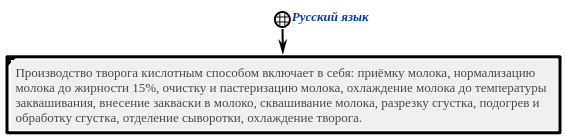
\includegraphics{Contents/part_kb/src/images/sd_natural_languages/nl_text.png}}
            \begin{scnindent}
            	\scntext{пояснение}{с точки зрения ostis-системы, любой естественно-языкой текст является \textit{файлом.}}
	            \scnrelfrom{лексическая структура}{\scnfileimage[20em]{Contents/part_kb/src/images/sd_natural_languages/nl_lexical.png}}
			    \begin{scnindent}
		            \scntext{пояснение}{Данная конструкция описывает декомпозицию исходного текста на фрагменты с указанием их принадлежности определённой \textit{номинативной единице} или \textit{знаку алфавита синтаксиса}.}
		            \scnrelfrom{синтаксическая структура}{\scnfileimage[20em]{Contents/part_kb/src/images/sd_natural_languages/nl_synactical.png}}
		            \scntext{пояснение}{Здесь приведена только частью синтаксической структуры. Оставшаяся часть записывается аналогично.}
		         \end{scnindent}
        	\end{scnindent}
        \end{scneqtoset}
    \end{scnsubstruct}
    \bigskip
    \scnendcurrentsectioncomment
\end{SCn}


\scparagraph[
    \protect\scneditors{Никифоров С.А.;Бобёр  Е.С.}
    \protect\scnmonographychapter{Глава 2.6. Языковые средства формального описания синтаксиса и денотационной семантики различных языков в интеллектуальных компьютерных системах нового поколения}
    ]{Предметная область и онтология синтаксиса естественных языков}
\label{sd_syntax_natural_lang}

\scparagraph[
    \protect\scneditors{Никифоров С.А.;Бобёр  Е.С.}
    \protect\scnmonographychapter{Глава 2.6. Языковые средства формального описания синтаксиса и денотационной семантики различных языков в интеллектуальных компьютерных системах нового поколения}
    ]{Предметная область и онтология денотационной семантики естественных языков}
\label{sd_sem_natural_lang}

\scsubsection[
    \protect\scneditors{Никифоров С.А.;Шункевич Д.В.}
    \protect\scnmonographychapter{Глава 3.1. Формализация понятий действия, задачи, метода, средства, навыка и технологии}
    ]{Глобальная предметная область и онтология, описывающая воздействия, действия, методы, средства и технологии}
\label{sd_actions}
\begin{SCn}

\scnsectionheader{\currentname}

\scnstartsubstruct

\scnheader{Предметная область и онтология действий, задач, планов, протоколов и методов}
\scniselement{предметная область}
\scnsdmainclasssingle{действие}
\scnsdclass{информационное действие;поведенческое действие;эффекторное действие;рецепторное действие;действие в sc-памяти;действие во внешней среде ostis-системы;эффекторное действие ostis-системы;рецепторное действие ostis-системы;инициированное действие;выполняемое действие;активное действие;отложенное действие;планируемое действие;выполненное действие;успешно выполненное действие;безуспешно выполненное действие;действие, выполненное с ошибкой;приоритет действия;субъект;внутренний субъект ostis-системы;внешний субъект ostis-системы, с которым осуществляется взаимодействие;внешний субъект ostis-системы, с которым взаимодействие не происходит;класс действий;атомарный класс действий;неатомарный класс действий;конъюнкция предшествующих действий;проверка условия;задача;процедурная формулировка задачи;декларативная формулировка задачи;класс задач;вопрос;команда;класс команд;класс команд без аргументов;класс команд с одним аргументом;класс команд с двумя аргументами;класс команд с произвольным числом аргументов;атомарный класс команд;неатомарный класс команд;план;программа;программа в sc-памяти;протокол;решение}
\scnsdrelation{дейcтвие с очень высоким приоритетом';дейcтвие с высоким приоритетом';дейcтвие со средним приоритетом';дейcтвие с низким приоритетом';дейcтвие с очень низким приоритетом';декомпозиция действия*;поддействие*;последовательность действий*;последовательность действий при положительном результате*;последовательность действий при отрицательном результате*;последовательность действий в случае ошибки* /*nrel\_error*/;результат*;исполнитель*;класс выполняемых действий*;заказчик*;инициатор*;объект*;контекст действия*;аргумент действия';первый аргумент действия’;второй аргумент действия’;третий аргумент действия’;класс аргументов*;класс первых аргументов*;класс вторых аргументов*}

\scnheader{действие}
\scnidtf{акция}
\scnidtf{сделать}
\scnidtf{работа}
\scnidtf{процесс выполнения некоторой работы}
\scnidtf{процесс решения некоторой задачи}
\scnidtf{процесс достижения некоторой цели}
\scnidtf{дело}
\scnidtf{мероприятие}
\scnidtf{воздействие}
\scnidtf{целостный фрагмент некоторой деятельности}
\scnidtf{целенаправленный процесс, управляемый некоторым субъектом}
\scnidtf{процесс выполнения некоторого действия некоторым субъектом (исполнителем) над некоторыми объектами}

\scnrelfrom{разбиение}{Разбиение класса действий по отношению к памяти информационной системы}
\scnaddlevel{1}
\scneqtoset{информационное действие\\
    \scnaddlevel{1}
    \scnrelfrom{включение}{действие в sc-памяти}
    \scnaddlevel{-1}
    ;поведенческое действие\\
    \scnaddlevel{1}
    \scnrelfrom{включение}{действие во внешней среде ostis-системы}
    \scnaddlevel{-1}
    ;эффекторное действие\\
    \scnaddlevel{1}
    \scnrelfrom{включение}{эффекторное действие ostis-системы}
    \scnaddlevel{-1}
    ;рецепторное действие\\
    \scnaddlevel{1}
    \scnrelfrom{включение}{рецепторное действие ostis-системы}
    \scnaddlevel{-1}}
\scnaddlevel{-1}

\scnrelfrom{разбиение}{Разбиение класса действий по отношению к текущему моменту времени}
\scnaddlevel{1}
\scneqtoset{инициированное  действие\\
    \scnaddlevel{1}
    \scnrelfrom{включение}{выполняемое действие\\
        \scnidtf{настоящее действие}\\
        \scnsubdividing{активное действие;отложенное действие}
    \scnaddlevel{-1}}
    ;планируемое действие\\
    \scnaddlevel{1}
    \scnidtf{будущее действие}
    \scnaddlevel{-1}
    ;выполненное действие\\
    \scnaddlevel{1}
    \scnidtf{прошлое действие}
    \scnsubdividing{успешно выполненное действие;безуспешно выполненное действие}
    \scnaddlevel{-1}}
\scnaddlevel{-1}
\scnexplanation{Каждое \textbf{\textit{действие}}, выполняемое тем или иным \textit{субъектом}, одновременно можно трактовать и как процесс решения некоторой задачи, т.е. как процесс достижения заданной цели в заданных условиях.

Предполагается, что любое \textbf{\textit{действие}}, выполняемое каким-либо \textit{субъектом}, направлено на решение какой-либо задачи и выполняется \uline{целенаправленно}. При \textit{этом} явное указание \textit{действия} и его связи с конкретной \textit{задачей} может не всегда присутствовать в памяти. Некоторые задачи могут решаться определенными агентами перманентно, например, оптимизация базы знаний, поиск некорректностей и т.д., и для подобных задач не всегда есть необходимость явно вводить \textit{структуру}, являющуюся формулировкой \textit{задачи}.

Каждое \textbf{\textit{действие}} может обозначать сколь угодно малое преобразование, осуществляемое во внешней среде либо в памяти некоторой системы, однако в памяти явно вводятся только знаки тех \textbf{\textit{действий}}, для которых есть необходимость явно хранить в памяти их спецификацию в течение некоторого времени.

При выполнении действия можно выделить следующие этапы:
\begin{scnitemize}
    \item построение плана деятельности; декомпозиция (детализация) исходного действия;
    \item выполнение построенного плана действий;
\end{scnitemize}}
\scntext{правило идентификации экземпляров}{Экземпляры класса \textbf{\textit{действий}} в рамках \textit{Русского языка} именуются по следующим правилам:
\begin{scnitemize}
    \item в начале идентификатора пишется слово \textbf{Действие} и ставится точка;
    \item далее с прописной буквы идет либо содержащее глагол совершенного вида в инфинитиве описание сути того, что требуется получить в результате выполнения действия, либо вопросительное предложение, являющееся спецификацией запрашиваемой (ответной) информации.
\end{scnitemize}
Например:\\
\textit{Действие. Сформировать полную семантическую окрестность понятия треугольник}\\
\textit{Действие. Верифицировать Раздел. Предметная область sc-элементов}
}

\scnheader{информационное действие}
\scnexplanation{Результатом выполнения \textbf{\textit{информационного действия}} является в общем случае некоторое новой состояние памяти информационной системы (не обязательно \textit{sc-памяти}), достигнутое исключительно путем преобразования информации, хранящейся в памяти системы, то есть либо посредством генерации новых знаний на основе уже имеющихся, либо посредством удаления знаний, по каким-либо причинам ставших ненужными. Следует отметить, что если речь идет об изменении состояния \textit{sc-памяти}, то любое преобразование информации можно свести к ряду элементарных действий генерации, удаления или изменения инцидентности \textit{sc-элементов} друг относительно друга.}

\scnheader{поведенческое действие}
\scnexplanation{В случае \textbf{\textit{поведенческого действия}} результатом его выполнения будет новое состояние внешней среды. Очень важно отметить, что под внешней средой в данном случае понимаются также и компоненты системы, внешние с точки зрения памяти, то есть не являющиеся хранимыми в ней информационными конструкциями. К таким компонентам можно отнести, например, различные манипуляторы и прочие средства воздействия системы на внешний мир, то есть к поведенческим задачам можно отнести изменение состояния механической конечности робота или непосредственно вывод некоторой информации на экран для восприятия пользователем.}

\scnheader{эффекторное действие}

\scnheader{рецепторное действие}

\scnheader{действие в sc-памяти}

\scnheader{действие во внешней среде ostis-системы}

\scnheader{эффекторное действие ostis-системы}

\scnheader{рецепторное действие ostis-системы}

\scnheader{инициированное действие}
\scnidtf{действие, подлежащее выполнению}
\scnidtf{действие, включенное в план}
\scnexplanation{Во множество \textbf{\textit{инициированных действий}} входят \textit{действия}, выполнение которых инициировано в результате какого-либо события.

В общем случае, \textit{действия} могут быть инициированы по следующим причинам:
\begin{scnitemize}
    \item \textit{действие} инициировано явно путем проведения соответствующей \textit{sc-дуги принадлежности} каким-либо \textit{субъектом} (\textit{заказчиком*}). В случае \textit{действия в sc-памяти}, оно может быть инициировано как внутренним \textit{sc-агентом} системы, так и пользователем при помощи соответствующего пользовательского интерфейса. При этом, спецификация действия может быть сформирована одним \textit{sc-агентом}, а собственно добавление во множество \textbf{\textit{инициированных действий}} может быть осуществлено позже другим \textit{sc-агентом}.
    \item \textit{действие} инициировано в результате того, что одно или несколько действий, предшествовавших данному в рамках некоторой декомпозиции, стали \textit{прошлыми сущностями} (процедурный подход).
    \item действие инициировано в результате того, что в памяти системы появилась конструкция, соответствующая некоторому условию инициирования \textit{sc-агента}, который должен выполнить данное \textit{действие} (декларативный подход)
\end{scnitemize}
Следует отметить, что декларативный и процедурный подходы можно рассматривать как две крайности, использование только одной из который не является удобным и целесообразным. При этом, например, принципы инициирования по процедурному подходу могут быть полностью сведены к набору декларативных условий инициирования, но как было сказано, это не всегда удобно и наиболее рациональным будет комбинировать оба похода в зависимости от ситуации.

По сути, попадание некоторого \textit{действия} во множество \textbf{\textit{инициированных действий}} говорит о том, что спецификация данного \textit{действия}, полностью сформирована, т.е. никаких дополнительных элементов, необходимых для решения поставленной задачи, не требуется, и соответствующий \textit{sc-агент} (либо коллектив \textit{sc-агентов}, либо внешний \textit{субъект}) может приступать к выполнению действия. Однако стоит отметить, что с точки зрения исполнителя такая спецификация \textit{действия} в общем случае может оказаться недостаточной или некорректной.}

\scnheader{выполняемое действие}
\scniselement{неосновное понятие}
\scnrelto{включение}{настоящая сущность}
\scnexplanation{Во множество \textbf{\textit{выполняемых действий}}  входят \textit{действия}, к выполнению которых приступил какой-либо из соответствующих \textit{субъектов}.

Попадание \textit{действия} в данное множество говорит о следующем:
\begin{scnitemize}
    \item рассматриваемое \textit{действие} уже попало во множество \textit{инициированных действий}.
    \item существует как минимум один \textit{субъект}, условие инициирования которого соответствует спецификации данного \textit{действия}.
\end{scnitemize}
После того, как собственно процесс выполнения завершился, \textit{действие} должно быть удалено из множества \textbf{\textit{выполняемых действий}} и добавлено во множество \textit{выполненных действий} или какое-либо из его подмножеств.

Понятие \textbf{\textit{выполняемое действие}} является неосновным, и вместо того, чтобы относить конкретные действия к данному классу, их относят к классу \textit{настоящих сущностей}.}

\scnheader{активное действие}
\scnexplanation{Во множество \textbf{\textit{активных действий}} входят \textit{действия}, выполнение которых осуществляется непосредственно в данный момент каким-либо \textit{субъектом}.}

\scnheader{отложенное действие}
\scnidtf{прерванное действие}
\scnidtf{приостановленное действие}
\scnexplanation{Во множество \textbf{\textit{отложенных действий}} входят \textit{действия}, которые уже были инициированы, однако их выполнение невозможно по каким-либо причинам, например в случае, когда у исполнителя в данный момент есть более приоритетные задачи.}

\scnheader{планируемое действие}
\scnidtf{будущее действие}
\scnexplanation{Во множество \textbf{\textit{планируемых действий}} входят \textit{действия}, начать выполнение которых запланировано на какой-либо момент в будущем.}

\scnheader{выполненное действие}
\scnidtf{прошлое действие}
\scniselement{неосновное понятие}
\scnrelto{включение}{прошлая сущность}
\scnexplanation{Во множество \textbf{\textit{выполненных действий}} попадают \textit{действия}, выполнение которых с точки зрения завершено с точки зрения \textit{субъекта}, осуществлявшего их выполнение. В зависимости от результатов конкретного процесса выполнения, рассматриваемое \textit{действие} может стать элементом одного из подмножеств множества \textbf{\textit{выполненных действий}}.

Понятие \textbf{\textit{выполненное действие}} является неосновным, и вместо того, чтобы относить конкретные \textit{действия} к данному классу, их относят к классу \textit{прошлых сущностей}.}

\scnheader{успешно выполненное действие}
\scnexplanation{Во множество \textbf{\textit{успешно выполненных действий}} попадают \textit{действия}, выполнение которых успешно завершено с точки зрения \textit{субъекта}, осуществлявшего их выполнение, т.е. достигнута поставленная цель, например, получены решение и ответ какой-либо задачи, успешно преобразована какая-либо конструкция и т.д.

Если действие было выполнено успешно, то, в случае действия по генерации каких-либо знаний, к \textit{действию} при помощи связки отношения \textit{результат*} приписывается \textit{sc-конструкция}, описывающая результат выполнения указанного действия. В случае, когда действие направлено на какие-либо изменения базы знаний, \textit{sc-конструкция}, описывающая результат действия, формируется в соответствии с правилами описания истории изменений базы знаний.

В случае, когда успешное выполнение \textit{действия} приводит к изменению какой-либо конструкции в \textit{sc-памяти}, которое необходимо занести в историю изменений базы знаний или использовать для демонстрации протокола решения задачи, то генерируется соответствующая связка отношения \textit{результат*}, связывающая \textit{задачу} и \textit{sc-конструкцию}, описывающую данное изменение.}

\scnheader{безуспешно выполненное действие}
\scnexplanation{Во множество \textbf{\textit{безуспешно выполненных действий}} попадают \textit{действия}, выполнение которых не было успешно завершено с точки зрения \textit{субъекта}, осуществлявшего их выполнение, по каким-либо причинам.

Можно выделить две основные причины, по которым может сложиться указанная ситуация:
\begin{scnitemize}
    \item соответствующая \textit{задача} сформулирована некорректно;
    \item формулировка соответствующей \textit{задачи} корректна и понятна системе, однако решение данной задачи в текущий момент не может быть получено за удовлетворительные с точки зрения заказчика или исполнителя сроки.
\end{scnitemize}
Для конкретизации факта некорректности формулировки задачи можно выделить ряд более частных классов \textbf{\textit{безуспешно выполненных действий}}, например:
\begin{scnitemize}
    \item \textit{действие}, спецификация которого противоречит другим знаниям системы (например, не выполняется неравенство треугольника);
    \item \textit{действие}, при спецификации которого использованы понятия, неизвестные системе;
    \item \textit{действие}, выполнение которого невозможно из-за недостаточности данных (например, найти площадь треугольника по двум сторонам);
    \item и другие
\end{scnitemize}
Для конкретизации факта безуспешности выполнения некоторого \textit{действия} в системе могут также использоваться дополнительные подмножества данного множества, при необходимости снабженные естественно-языковыми комментариями.}
\scnrelfrom{включение}{действие, выполненное с ошибкой}

\scnheader{действие, выполненное с ошибкой}
\scnexplanation{Во множество \textbf{\textit{действий, выполненных с ошибкой}}, попадают \textit{действия}, выполнение которых не было успешно завершено с точки зрения \textit{субъекта}, осуществлявшего их выполнение, по причине возникновении какой-либо ошибки, например, некорректности спецификации данного \textit{действия} или нарушении ее целостности каким-либо \textit{субъектом} (в случае \textit{действия в sc-памяти}).}

\scnheader{приоритет действия}
\scnhaselement{дейcтвие с очень высоким приоритетом'}
\scnhaselement{дейcтвие с высоким приоритетом'}
\scnhaselement{дейcтвие со средним приоритетом'}
\scnhaselement{дейcтвие с низким приоритетом'}
\scnhaselement{дейcтвие с очень низким приоритетом'}
\scnexplanation{Множество \textbf{\textit{приоритет действия}} представляет собой семейство ролевых отношений, элементами которых являются \textit{sc-дуги принадлежности}, связывающие множество поддействий в рамках декомпозиции некоторого более сложного \textit{действия} и сами эти поддействия. Таким образом, данные ролевые отношения задают приоритетность выполнения более частных поддействий при выполнении некоторого общего действия. Приоритетность выполнения влияет на \textit{действия}, независимые с точки зрения \textit{последовательности действий*}, и отражает влияние каждого более частного действия на качество результата выполнения общего действия.}

\scnheader{дейcтвие с очень высоким приоритетом'}

\scnheader{дейcтвие с высоким приоритетом'}

\scnheader{дейcтвие со средним приоритетом'}

\scnheader{дейcтвие с низким приоритетом'}

\scnheader{дейcтвие с очень низким приоритетом'}

\scnheader{субъект}
\scnidtf{активная сущность}
\scnidtf{сущность, способная самостоятельно выполнять некоторые виды действий}
\scnidtf{агент деятельности}
\scnrelfromlist{включение}{Собственное Я;внутренний субъект ostis-системы;внешний субъект ostis-системы, с которым осуществляется взаимодействие;внешний субъект ostis-системы, с которым взаимодействие не происходит}

\scnheader{внутренний субъект ostis-системы}
\scnidtf{субъект, входящий в состав той ostis-системы, в базе знаний которой он описывается}
\scnrelfrom{включение}{sc-агент}
\scnexplanation{Под \textbf{\textit{внутренним субъектом ostis-системы}} понимается такой \textit{субъект}, который выполняет некоторые \textit{действия} в \uline{той же памяти}, в которой хранится его знак.\\
К числу \textbf{\textit{внутренних субъектов ostis-системы}} относятся входящие в нее \textit{sc-агенты}, частные sc-машины, целые интеллектуальные подсистемы.}

\scnheader{внешний субъект ostis-системы, с которым осуществляется взаимодействие}
\scnexplanation{К числу \textbf{\textit{внешних субъектов ostis-системы, с которыми осуществляется взаимодействие}}, относятся конечные пользователи \textit{ostis-системы}, ее разработчики, а также другие компьютерные системы (причем, не только интеллектуальные).}

\scnheader{внешний субъект ostis-системы, с которым взаимодействие не происходит}

\scnheader{класс действий}
\scnidtf{множество действий, однотипных в том или ином смысле}
\scnrelto{семейство подмножеств}{действие}
\scnsubdividing{атомарный класс действий;неатомарный класс действий}
\scntext{правило идентификации экземпляров}{Конкретные \textbf{\textit{классы действий}} в рамках \textit{Русского языка} именуются по следующим правилам:
\begin{scnitemize}
    \item в начале идентификатора пишется слово \textbf{действие} и ставится точка;
    \item далее со строчной буквы идет либо содержащее глагол совершенного вида в инфинитиве описание сути того, что требуется получить в результате выполнения действий данного класса, либо вопросительное предложение, являющееся спецификацией запрашиваемой (ответной) информации.
\end{scnitemize}
Например:\\
\textit{действие. сформировать полную семантическую окрестность указываемой сущности}\\
\textit{действие. верифицировать заданную sc-структуру}

Допускается использовать менее строгие идентификаторы, которые, однако, обязаны оперировать словом \textbf{\textit{действие}} и достаточно четко специфицировать суть действий описываемого класса. 

Например:\\
\textit{действие редактирования базы знаний}\\
\textit{действие, направленное на установление темпоральных характеристик указываемой сущности}}

\scnheader{атомарный класс действий}
\scnexplanation{Принадлежность некоторого \textit{класса действий} множеству \textbf{\textit{атомарных классов действий}} фиксирует факт того, что при указании всех необходимых аргументов принадлежности \textit{действия} данному классу достаточно для того, чтобы некоторый субъект мог приступить к выполнению этого действия.

При этом, даже если \textit{класс действий} принадлежит множеству \textbf{\textit{атомарных классов действий}}, не запрещается вводить более частные \textit{классы действий}, для которых, например, заранее фиксируется один из аргументов.

Если конкретный \textbf{\textit{атомарный класс действий}} является более частным по отношению к \textit{действиям в sc-памяти}, то это говорит о наличии в текущей версии системы как минимум одного \textit{sc-агента}, ориентированного на выполнение действий данного класса.}

\scnheader{неатомарный класс действий}
\scnexplanation{Принадлежность некоторого \textit{класса действий} множеству \textbf{\textit{неатомарных классов действий}} фиксирует факт того, что даже при указании всех необходимых аргументов принадлежности \textit{действия} данному классу недостаточно для того, чтобы некоторый \textit{субъект} приступил к выполнению этого действия, и требуются дополнительные уточнения.}

\scnheader{декомпозиция действия*}
\scnidtf{сведение действия ко множеству более простых взаимосвязанных действий*}
\scnexplanation{Связки отношения \textbf{\textit{декомпозиция действия*}} связывают \textit{действие}, и множество частных \textit{действий}, на которые декомпозируется данное \textit{действие}. При этом первым компонентом связки является знак указанного множества, вторым компонентом – знак более общего \textit{действия}.

Таким образом, \textbf{\textit{декомпозиция действия*}} это \textit{квазибинарное отношение}, связывающее действие со множеством действий более низкого уровня, к выполнению которых сводится выполнение исходного декомпозируемого действия.

Стоит отметить, что каждое \textit{действие} может иметь несколько вариантов декомпозиции в зависимости от конкретного набора элементарных действий, которые способна выполнять та или иная система \textit{субъектов}.

Принцип, по которому осуществляется такая декомпозиция в различных подходах к решению задач будем называть \textit{стратегией решения задач}.}
\scniselement{отношение декомпозиции}
\scniselement{квазибинарное отношение}

\scnheader{поддействие*}
\scnidtf{частное действие*}
\scnrelto{включение}{темпоральная часть*}
\scnexplanation{Связки отношения \textbf{\textit{поддействие*}} связывают \textit{действие}, и некоторое более простое частное \textit{действие}, выполнение которого необходимо для выполнения исходного более общего \textit{действия}.}
\scniselement{бинарное отношение}
\scniselement{отношение таксономии}

%\addedstart
\scnheader{абстрактное поддействие*}
\scniselement{бинарное отношение}
\scniselement{отношение таксономии}
%\addedend

\scnheader{последовательность действий*}
\scnidtf{порядок действий*}
\scnidtf{бинарная ориентированная связка, описывающая то, какое действие может быть инициировано после завершения выполнения другого (предшествующего)*}
\scnidtf{бинарная ориентированная связка, описывающая передачу управления от одного (предшествующего) действия к другому (последующему)*}
\scnidtf{goto*}
\scniselement{отношение порядка}
\scnexplanation{Связки отношения \textbf{\textit{последовательность действий*}} связывают знаки \textit{действий}, выполняющихся в какой-либо последовательности в процессе решения какой-либо задачи. При этом считается, что если два \textit{действия} связаны данным отношением, то \textit{действие}, стоящее в данной связке на втором месте может быть выполнено только после выполнения \textit{действия}, стоящего в данной связке на первом месте. Таким образом, каждое действие может быть инициировано после завершения выполнения любого из предшествующих действий.

Для обеспечения возможности синхронизации выполнения действий используется класс действий \textit{конъюнкция предшествующих действий}.

При этом дополнительно может указываться абсолютный \textit{приоритет действия}, характеризующий принципиальную важность действия и срочность его выполнения, не всегда зависящую напрямую от других действий, но при этом влияющую на порядок выполнения действий из некоторого множества в целом.}
\scnrelfromlist{включение}{последовательность действий при положительном результате*;последовательность действий при отрицательном результате*;последовательность действий в случае ошибки*}

\scnheader{конъюнкция предшествующих действий}
\scnidtf{действие, заключающееся только в ожидании установлении факта завершения всех предшествующих действий}
\scnrelto{включение}{действие}
\scnexplanation{Действия класса \textbf{\textit{конъюнкция предшествующих действий}} используются в тех случаях, когда выполнение некоторого действия должно начаться только после того, как будут выполнены все предшествующие действия, а не только одно из них. После того, как все предшествующие действия выполнены, инициируются действия, следующие за \textbf{\textit{конъюнкцией предшествующих действий}}.}

\scnheader{проверка условия}
\scnidtf{if-действие}
\scnidtf{действие, направленное на установление истинности или ложности заданного высказывания}
\scnrelto{включение}{действие}
\scnexplanation{Действия класса \textbf{\textit{проверка условия}} предполагают проверку истинности или ложности некоторого высказывания (условия), и после выполнения в зависимости от результата данной проверки становятся \textit{успешно выполненными действиями} или \textit{безуспешно выполненными действиями}.}

\scnheader{последовательность действий при положительном результате*}
\scnidtf{then*}
\scniselement{отношение порядка}
\scnexplanation{Переход по связкам отношения \textbf{\textit{последовательность действий при положительном результате*}} от предшествующего действия проверки условия к последующему действию происходит при условии, если указанная проверка даст положительный результат, то есть предшествующее действие станет \textit{успешно выполненным действием}.}

\scnheader{последовательность действий при отрицательном результате*}
\scnidtf{else*}
\scniselement{отношение порядка}
\scnexplanation{Переход по связкам отношения \textbf{\textit{последовательность действий при отрицательном результате*}} от предшествующего действия проверки условия к последующему действию происходит при условии, если указанная проверка даст отрицательный результат, то есть предшествующее действие станет \textit{безуспешно выполненным действием}.}

\scnheader{последовательность действий в случае ошибки* /*nrel\_error*/}
\scnidtf{error*}
\scniselement{отношение порядка}
\scnexplanation{Переход по связкам отношения \textbf{\textit{последовательность действий в случае ошибки*}} от предшествующего \textit{действия} к последующему \textit{действию} происходит в случае, когда выполнение предыдущего \textit{действия} не может быть завершено при возникновении какой-либо ошибки, например, некорректности спецификации данного \textit{действия} или нарушении ее целостности каким-либо субъектом (в случае \textit{действия в sc-памяти}).}

\scnheader{результат*}
\scnidtf{цель*}
\scnexplanation{Связки отношения \textbf{\textit{результат*}} связывают \textit{sc-элемент}, обозначающий \textit{действие}, и \textit{sc-конструкцию}, описывающую результат выполнения рассматриваемого действия, другими словами, цель, которая должна быть достигнута при выполнении \textit{действия}.\\
Результат может специфицироваться как атомарным высказыванием, так и неатомарным, т.е. конъюнктивным, дизъюнктивным, строго дизъюнктивным и т.д.\\
В случае, когда успешное выполнение \textit{действия} приводит к изменению какой-либо конструкции в \textit{sc-памяти}, которое необходимо занести в историю изменений базы знаний или использовать для демонстрации протокола решения задачи, генерируется соответствующая связка отношения \textbf{\textit{результат*}}, связывающая \textit{задачу} и \textit{sc-конструкцию}, описывающую данное изменение. Конкретный вид указанной \textit{sc-конструкции} зависит от типа действия.}

\scnheader{задача}
\scnidtf{sc-описание некоторого желаемого состояния или события либо в базе знаний, либо во внешней среде}
\scnidtf{формулировка задачи}
\scnidtf{задание на выполнение некоторого действия}
\scnidtf{постановка задачи}
\scnidtf{описание задачной ситуации}
\scnidtf{спецификация некоторого действия, обладающая достаточной полнотой для выполнения этого действия}
\scnidtf{цель плюс дополнительные условия (ограничения) накладываемые на результат или процесс получения этого результата}
\scnidtf{описание того, что требуется сделать}
\scnexplanation{Под \textbf{\textit{задачей}} понимается формальное описание условия некоторой задачи, то есть, по сути, формальная спецификация некоторого действия, направленного на решение данной задачи, достаточная для выполнения данного действия каким-либо \textit{субъектом}. В зависимости от конкретного класса задач, описываться может как внутреннее состояние самой интеллектуальной системы, так и требуемое состояние внешней среды. \textit{sc-элемент}, обозначающий \textit{действие} входит в \textit{задачу} под атрибутом \textit{ключевой sc-элемент'}.

Каждая \textbf{\textit{задача}} представляет собой спецификацию действия, которое либо уже выполнено, либо выполняется в текущий момент (в настоящее время), либо планируется (должно) быть выполненным, либо может быть выполнено (но не обязательно).

Классификация задач может осуществляться по дидактическому признаку в рамках каждой предметной области, например, задачи на треугольники, задачи на системы уравнений и т.п.

Каждая \textit{задача} может включать:
\begin{scnitemize}
    \item факт принадлежности \textit{действия} какому-либо частному классу \textit{действий} (например,\textit{ действие. сформировать полную семантическую окрестность указываемой сущности}), в том числе состояние \textit{действия} с точки зрения жизненного цикла (инициированное, выполняемое и т.д.);
    \item описание \textit{цели*} (\textit{результата*}) \textit{действия}, если она точно известна;
    \item указание \textit{заказчика*} действия;
    \item указание \textit{исполнителя* действия} (в том числе, коллективного);
    \item указание \textit{аргумента(ов) действия’};
    \item указание инструмента или посредника \textit{действия};
    \item описание \textit{декомпозиции действия*};
    \item указание \textit{последовательности действий*} в рамках \textit{декомпозиции действия*}, т.е построение плана решения задачи. Другими словами, построение плана решения представляет собой декомпозицию соответствующего \textit{действия} на систему взаимосвязанных между собой поддействий;
    \item указание области \textit{действия};
    \item указание условия инициирования \textit{действия};
    \item момент начала и завершения \textit{действия}, в том числе планируемый и фактический, предполагаемая и/или фактическая длительность выполнения;
\end{scnitemize}
Некоторые задачи могут быть дополнительно уточнены контекстом – дополнительной информацией о сущностях, рассматриваемых в формулировке \textit{задачи}, т.е. описанием того, что дано, что известно об указанных сущностях.

Построение плана решения задачи это декомпозиция спецификации процесса решения заданной задачи на систему 
 
Кроме этого, \textit{задача} может включать любую дополнительную информацию о действии, например:
\begin{scnitemize}
    \item перечень ресурсов и средств, которые предполагается использовать при решении задачи, например список доступных исполнителей, временные сроки, объем имеющихся финансов и т.д.;
    \item ограничение области, в которой выполняется \textit{действие}, например, необходимо заменить одну \textit{sc-конструкцию} на другую по некоторому правилу, но только в пределах некоторого \textit{раздела базы знаний};
    \item ограничение знаний, которые можно использовать для решения той или иной задачи, например, необходимо решить задачу по алгебре используя только те утверждения, которые входят в курс школьной программы до седьмого класса включительно, и не используя утверждения, изучаемые в старших классах;
    \item и прочее
\end{scnitemize}
С одной стороны, решаемые системой задачи, можно классифицировать на \textit{информационные задачи} и \textit{поведенческие задачи}. 

С точки зрения формулировки поставленной задачи можно выделить \textit{декларативные формулировки задачи} и \textit{процедурные формулировки задачи}. Следует отметить, что данные классы задач не противопоставляются, и могут существовать формулировки задач, использующие оба подхода.}
\scntext{правило идентификации экземпляров}{Экземпляры класса \textbf{\textit{задач}} в рамках \textit{Русского языка} именуются по следующим правилам:
\begin{scnitemize}
    \item в начале идентификатора пишется слово \textbf{Задача} и ставится точка;
    \item далее с прописной буквы идет либо содержащее глагол совершенного вида в инфинитиве описание сути того, что требуется получить в результате выполнения действия, либо вопросительное предложение, являющееся спецификацией запрашиваемой (ответной) информации.
\end{scnitemize}
Например:\\
\textit{Задача. Сформировать полную семантическую окрестность понятия треугольник}\\
\textit{Задача. Верифицировать Раздел. Предметная область sc-элементов}}
\scnrelto{включение}{семантическая окрестность}
\scnrelfromlist{включение}{процедурная формулировка задачи;декларативная формулировка задачи
}
\scnrelfromlist{включение}{вопрос;команда}

\scnheader{процедурная формулировка задачи}
\scnidtf{спецификация действия, которое планируется быть выполненным}
\scnexplanation{В случае \textbf{\textit{процедурной формулировки задачи}}, в формулировке задачи явно указываются аргументы соответствующего задаче \textit{действия}, и в частности, вводится семантическая типология \textit{действий}. При этом явно не уточняется, что должно быть результатом выполнения данного действия. Заметим, что, при необходимости, \textit{процедурная формулировка задачи} может быть сведена к \textit{декларативной формулировке задачи} путем трансляции на основе некоторого правила, например определения класса действия через более общий класс.}

\scnheader{декларативная формулировка задачи}
\scnidtf{описание ситуации (состояния), которое должно быть достигнуто в результате выполнения планируемого действия}
\scnexplanation{В случае \textit{декларативной формулировки задачи}, при описании условия задачи специфицируется цель \textit{действия}, т.е. результат, который должен быть получен при успешном выполнении \textit{действия}.}

\scnheader{класс задач}
\scnrelto{семейство подмножеств}{задача}
\scntext{правило идентификации экземпляров}{Конкретные \textbf{\textit{классы задач}} в рамках \textit{Русского языка} именуются по следующим правилам:
\begin{scnitemize}
    \item в начале идентификатора пишется слово \textbf{задача} и ставится точка;
    \item далее с прописной буквы идет либо содержащее глагол совершенного вида в инфинитиве описание сути того, что требуется получить в результате решения данного \textbf{\textit{класса задач}}, либо вопросительное предложение, являющееся спецификацией запрашиваемой (ответной) информации.
\end{scnitemize}
Например:\\
\textit{задача. сформировать полную семантическую окрестность указываемой сущности}\\
\textit{задача. верифицировать заданную sc-структуру}

Допускается использовать менее строгие идентификаторы, которые, однако, обязаны оперировать словом \textbf{задача} и достаточно четко специфицировать суть задач описываемого класса. 

Например:\\
\textit{задача на установление значения величины}\\
\textit{задача на доказательство}
}

\scnheader{вопрос}
\scnidtf{задача, направленная на удовлетворение информационной потребности некоторого субъекта-заказчика}

\scnheader{команда}
\scnidtf{инициированная задача}
\scnidtf{спецификация инициированного действия}
\scnexplanation{Идентификатор экземпляров конкретного класса \textbf{\textit{команд}} в рамках \textit{Русского языка} пишется с прописной буквы и представляет собой либо содержащее глагол совершенного вида в инфинитиве описание сути того, что требуется получить в результате выполнения действия, соответствующего данной \textbf{\textit{команде}}, либо вопросительное предложение, являющееся спецификацией запрашиваемой (ответной) информации. 

Например:\\
\textit{Сформировать полную семантическую окрестность понятия треугольник}\\
\textit{Верифицировать Раздел. Предметная область sc-элементов}
}

\scnheader{класс команд}
\scnrelto{семейство подмножеств}{задача}
\scnrelfromlist{включение}{класс интерфейсных пользовательских команд\\
    \scnaddlevel{1}
    \scnrelfromlist{включение}{класс интерфейсных команд пользователя ostis-системы}
    \scnaddlevel{-1}}
\scnrelfromlist{включение}{класс команд без аргументов;класс команд с одним аргументом;класс команд с двумя аргументами;класс команд с произвольным числом аргументов}
\scnexplanation{Идентификатор конкретного класса \textbf{\textit{класса команд}} в рамках \textit{Русского языка} пишется со строчной буквы и представляет собой либо содержащее глагол совершенного вида в инфинитиве описание сути того, что требуется получить в результате выполнения действий, соответствующих данному \textbf{\textit{классу команд}}, либо вопросительное предложение, являющееся спецификацией запрашиваемой (ответной) информации. 

Например:\\
\textit{сформировать полную семантическую окрестность указываемой сущности}\\
\textit{верифицировать заданную sc-структуру}

Допускается использовать менее строгие идентификаторы, которые, однако, обязаны оперировать словом \textbf{команда} и достаточно четко специфицировать суть задач описываемого класса. 

Например:\\
\textit{команда редактирования базы знаний}\\
\textit{команда установления темпоральных характеристик указываемой сущности}}
\scnsubdividing{атомарный класс команд;неатомарный класс команд}

\scnheader{класс команд без аргументов}

\scnheader{класс команд с одним аргументом}

\scnheader{класс команд с двумя аргументами}

\scnheader{класс команд с произвольным числом аргументов}

\scnheader{атомарный класс команд}
\scnexplanation{Принадлежность некоторого \textit{класса команд} множеству \textbf{\textit{атомарных классов команд}} фиксирует факт того, что данная спецификация является достаточной для того, чтобы некоторый субъект приступил к выполнению соответствующего действия.

При этом, даже если \textit{класса команд} принадлежит множеству \textbf{\textit{атомарных классов команд}} не запрещается вводить более частные \textit{классы команд}, в состав которых входит информация, дополнительно специфицирующая соответствующее \textit{действие}.

Если соответствующий данному \textit{классу команд класс действий} является более частным по отношению к \textit{действиям в sc-памяти}, то попадание данного класса команд во множество \textbf{\textit{атомарных классов команд}} говорит о наличии в текущей версии системы как минимум одного \textit{sc-агента}, условие инициирования которого соответствует формулировке команд данного класса.}

\scnheader{неатомарный класс команд}
\scnexplanation{Принадлежность некоторого \textit{класса команд} множеству \textbf{\textit{неатомарных классов команд}} фиксирует факт того, что данная спецификация не является достаточной для того, чтобы некоторый субъект приступил к выполнению соответствующего действия, и требует дополнительных уточнений.}

\scnheader{план}
\scnidtf{план выполнения}
\scnidtf{план решения}
\scnrelto{включение}{знание}
\scnexplanation{Каждый \textbf{\textit{план}} представляет собой \textit{семантическую окрестность}, \textit{ключевым sc-элементом'} является \textit{действие}, для которого дополнительно детализируется предполагаемый процесс его выполнения. Основная задача такой детализации – локализация области базы знаний, в которой предполагается работать, а также набора агентов, необходимого для выполнения описываемого действия. При этом детализация не обязательно должна быть доведена до уровня элементарных действий, цель составления плана – уточнение подхода к решению той или иной задачи, не всегда предполагающее составления подробного пошагового решения.

При описании \textbf{\textit{плана}} может быть использован как процедурный, так и декларативный подход. В случае процедурного подхода для соответствующего \textit{действия} указывается его декомпозиция на более частные поддействия, а также необходимая спецификация этих поддействий. В случае декларативного подхода указывается набор подцелей (например, при помощи логических утверждений), достижение которых необходимо для выполнения рассматриваемого \textit{действия}. На практике оба рассмотренных подхода можно комбинировать.

В общем случае \textbf{\textit{план}} может содержать и переменные, например в случае, когда часть плана задается в виде цикла (многократного повторения некоторого набора действий). Также план может содержать константы, значение которых в настоящий момент не установлено и станет известно, например, только после выполнения предшествующих ему \textit{действий}.

Каждый \textbf{\textit{план}} может быть задан заранее как часть спецификации \textit{действия}, т.е. \textit{задачи}, а может формироваться \textit{субъектом} уже собственно в процессе выполнения \textit{действия}, например, в случае использования стратегии разбиения задачи на подзадачи. В первом случае \textbf{\textit{план}} \textit{включается*} в \textit{задачу}, соответствующую тому же действию.}

\scnheader{программа}
\scnidtf{программа выполнения действий некоторого класса}
\scnidtf{обобщенный план}
\scnidtf{обобщенный план выполнения некоторого класса действий}
\scnidtf{обобщенный план решения некоторого класса задач}
\scnidtf{обобщенная спецификация декомпозиции любого действия, принадлежащего заданному классу действий}
\scnidtf{знание о некотором классе действий (и соответствующем классе задач), позволяющее для каждого из указанных действий достаточно легко построить план его выполнения}
\scnrelto{включение}{знание}
\scnrelfrom{включение}{программа в sc-памяти}
\scnexplanation{Каждая \textbf{\textit{программа}} представляет собой обобщенный план выполнения \textit{действий}, принадлежащих некоторому классу, то есть \textit{семантическую окрестность, ключевым sc-элементом'} является \textit{класс действий}, для элементов которого дополнительно детализируется процесс их выполнения.

В остальном описание \textbf{\textit{программы}} аналогично описанию \textit{плана} выполнения конкретного \textit{действия} из рассматриваемого \textit{класса действий}.

Одному \textit{классу действий} может соответствовать несколько \textbf{\textit{программ}}.

Входным параметрам \textbf{\textit{программы}} в традиционном понимании соответствуют аргументы, соответствующие каждому \textit{действию} из \textit{класса действий}, описываемого \textbf{\textit{программой}}. При генерации на основе \textbf{\textit{программы}} \textit{плана} выполнения конкретного \textit{действия} из данного класса эти аргументы принимают конкретные значения.

Каждая \textbf{\textit{программа}} представляет собой систему описанных действий с дополнительным указанием для действия:
\begin{scnitemize}
    \item либо \textit{последовательности выполнения действий*} (передачи инициирования), когда условием выполнения (инициирования) действий является завершение выполнения одного из указанных или всех указанных действий;
    \item либо события в базе знаний или внешней среде, являющегося условием его инициирования;
    \item либо ситуации в базе знаний или внешней среде, являющейся условием его инициирования;
\end{scnitemize}
}

\scnheader{программа в sc-памяти}

\scnheader{протокол}
\scnexplanation{Каждый \textbf{\textit{протокол}} представляет собой \textit{семантическую окрестность, ключевым sc-элементом'} является \textit{действие}, для которого собственно описывается весь процесс его выполнения, то есть все более простые поддействия, в том числе те, выполнение которых, как выяснилось позже, не было целесообразным. Подразумевается, что \textit{sc-элемент}, обозначающий данное действие, входит во множество прошлых сущностей.

Таким образом, \textbf{\textit{протокол}} представляет собой \textit{sc-текст}, содержащий декомпозицию рассматриваемого \textit{действия} на поддействия с указанием порядка их выполнения, а также необходимой спецификацией каждого такого поддействия.

В отличие от \textit{плана}, \textbf{\textit{протокол}} всегда формируется по факту выполнения соответствующего \textit{действия}.}

\scnheader{решение}
\scnexplanation{Каждое \textbf{\textit{решение}} представляет собой \textit{семантическую окрестность, ключевым sc-элементом'} является \textit{действие}, для которого собственно описывается процесс его выполнения, то есть решение соответствующей задачи. Подразумевается, что \textit{sc-элемент}, обозначающий данное \textit{действие}, входит во множество \textit{успешно выполненных действий}.

Таким образом, \textbf{\textit{решение}} представляет собой \textit{sc-текст}, содержащий декомпозицию рассматриваемого \textit{действия} на поддействия с указанием порядка их выполнения, а также необходимой спецификацией каждого такого поддействия.

Стоит отметить, что в случае отношения \textbf{\textit{решение*}} в \textit{декомпозиции действия*} указываются только те поддействия, без которых решение поставленной задачи было бы невозможным, то есть из \textit{протокола} исключаются ложные или избыточные шаги, проделанные в процессе поиска пути решения задачи, которые, в свою очередь, могут присутствовать при описании непосредственно текущего хода решения задачи.

Для конкретного \textit{действия} его \textbf{\textit{решение}} будет нестрого \textit{включаться*} в соответствующий \textit{протокол} решения.}

\scnheader{исполнитель*}
\scnexplanation{Связки отношения \textbf{\textit{исполнитель*}} связывают \textit{sc-элементы}, обозначающие \textit{действие} и \textit{sc-элементы}, обозначающие \textit{субъекта}, который предположительно будет осуществлять, осуществляет или осуществлял выполнение указанного \textit{действия}. Данное отношение может быть использовано при назначении конкретного исполнителя для проектной задачи по развитию баз знаний.

В случае, когда заранее неизвестно, какой именно \textit{субъект*} будет исполнителем данного \textit{действия}, связка отношения \textbf{\textit{исполнитель*}} может отсутствовать в первоначальной формулировке \textit{задачи} и добавляться позже, уже непосредственно при исполнении.

Когда действие выполняется (является \textit{настоящей сущностью}) или уже выполнено (является \textit{прошлой сущностью}), то исполнитель этого действия в каждый момент времени уже определен. Но когда действие только инициировано, тогда важно знать:
\begin{scnenumerate}
    \item кто \uline{хочет} выполнить это действие и насколько важно для него стать исполнителем данного действия;
    \item кто \uline{может} выполнить данное действие и каков уровень его квалификации и опыта;
    \item кто и кому поручает выполнить это действие и каков уровень ответственности за невыполнение (приказ, заказ, официальный договор, просьба…);
\end{scnenumerate}

При этом следует помнить, что связь отношения \textit{исполнитель*} в данном случае также является временной прогнозируемой сущностью.

Первым компонентом связок отношения \textit{исполнитель*} является знак \textit{действия}, вторым - знак \textit{субъекта}-исполнителя.}

\scnheader{класс выполняемых действий*}
\scnidtf{класс действий, выполняемых классом субъектов*}
\scnexplanation{Связки отношения \textbf{\textit{класс выполняемых действий*}} связывают классы субъектов и классы действий, при этом предполагается, что каждый субъект указанного класса способен выполнять действия указанного класса действий.}

\scnheader{заказчик*}
\scnexplanation{Связки отношения \textbf{\textit{заказчик*}} связывают \textit{sc-элементы}, обозначающие \textit{действие} и \textit{sc-элементы}, обозначающие \textit{субъекта}, который «заинтересован» в выполнении данного действия и, как правило, инициирует его выполнение. Данное отношение может быть использовано при указании того, кто поставил проектную задачу по развитию баз знаний.

Первым компонентом связок отношения \textbf{\textit{заказчик*}} является знак \textit{действия}, вторым - знак \textit{субъекта}-заказчика.}

\scnheader{инициатор*}
\scnexplanation{Связки отношения \textbf{\textit{инициатор*}} связывают \textit{sc-элемент}, обозначающий \textit{инициированное действие}, и знак \textit{субъекта}, который является инициатором данного \textit{действия}, то есть \textit{субъектом}, который инициировал данное \textit{действие} и, как правило, заинтересован в его успешном выполнении.}

\scnheader{объект*}
\scnexplanation{Связки отношения \textbf{\textit{объект*}} связывают \textit{sc-элемент}, обозначающий \textit{действие}, и знак той сущности, над которой (по отношению к которой) осуществляется данное \textit{действие}, например знак \textit{структуры}, подлежащий верификации.}

\scnheader{контекст действия*}
\scnidtf{задачная ситуация*}
\scnidtf{что дано*}
\scnidtf{дополнительная информация о тех сущностях, которые входят в описание цели*}
\scnidtf{связь между некоторой задачей (формулировкой задачи) и состоянием базы знаний, возможностей и навыков некоторого субъекта, перед которым поставлена указанная задача*}
\scnidtf{связь между формулировкой задачи, т.е. описанием того, что требуется, и контекстом этой задачи, т.е. описанием имеющихся ресурсов, описанием того, что дано*}
\scnexplanation{Связки отношения \textbf{\textit{контекст действия*}} связывают \textit{sc-элементы}, обозначающие \textit{действие} и \textit{sc-структуры}, обозначающие контекст выполнения данного \textit{действия}, то есть некоторую дополнительную информации о тех сущностях, которые входят в описание \textit{цели*}. Как правило, контекст используется для указания собственно условия некоторой задачи, того, что дано, т.е. тех знаний, которые можно использовать для вывода новых знаний при решении задачи. Таким образом, контекст непосредственно влияет на то, как будет решаться та или иная задача, при этом даже задачи соответствующие одному классу действий, могут решаться по-разному.

Контекст может быть представлен не только в виде атомарного фактографического высказывания, но и в виде высказывания более сложного вида. Это может быть, например:
\begin{scnitemize}
    \item определение множества, используемого в описании \textit{цели*};
    \item утверждение, учет которого может быть полезен в решении задач;    
\end{scnitemize}
Первым компонентом связок отношения \textbf{\textit{контекст действия*}} является знак \textit{действия}, вторым - знак \textit{sc-структуры}, обозначающей контекст.}

\scnheader{аргумент действия'}
\scniselement{ролевое отношение}
\scnexplanation{Связки ролевого отношения \textbf{\textit{аргумент действия’}} указываются в рамках конкретного действия те \textit{sc-элементы}, которые обозначают непосредственно аргументы данного \textit{действия}, если они явно указываются (в случае процедурной формулировки задачи).}
\scnrelfromlist{включение}{первый аргумент действия’;второй аргумент действия’;третий аргумент действия’}

\scnheader{первый аргумент действия’}

\scnheader{второй аргумент действия’}

\scnheader{третий аргумент действия’}

\scnheader{класс аргументов*}
\scnidtf{класс аргументов класса команд*}
\scnidtf{быть классом sc-элементов, экземпляры которого являются аргументами для заданного класса команд*}
\scnrelfromlist{включение}{класс первых аргументов*;класс вторых аргументов*}
\scnexplanation{Связки отношения \textbf{\textit{класс аргументов*}} связывают \textit{классы команд} (подмножества множества \textit{команд}), и классы \textit{sc-элементов}, которые могут быть аргументами действий, соответствующих данному \textit{классу команд}. В случае, когда \textit{команды} данного класса имеют один аргумент, используется собственно отношение \textbf{\textit{класс аргументов*}}, в случае, когда больше команды данного класса имеют более одного аргумента, то используются подмножества данного отношения, такие как \textit{класс первых аргументов*}, \textit{класс вторых аргументов*} и т.д.

Если для некоторого \textit{класса команд} не указан тип какого-либо из аргументов, то предполагается, что в качестве данного аргумента может выступать любой \textit{sc-элемент}.

Первым компонентом связок отношения \textbf{\textit{класс аргументов*}} является знак \textit{класса команд}, вторым – знак класса \textit{sc-элементов}, которые могут быть \textit{аргументами действий'}, соответствующих данному \textit{классу команд}.}

\scnheader{класс первых аргументов*}

\scnheader{класс вторых аргументов*}

\scnendstruct

\end{SCn}

\scsubsubsection[
    \protect\scnmonographychapter{Глава 3.1. Формализация понятий действия, задачи, метода, средства, навыка и технологии}
    ]{Предметная область и онтология локальных предметных областей и онтологий действий}
\label{local_sd_actions}

\scsubsubsection[
    \protect\scnidtf{Типология неавтоматизированных (\scnqq{вручную} выполняемых) и автоматически выполняемых \textit{действий}, направленных на управление процессами выполнения различных \textit{сложных действий}, а также система понятий, используемая для \textit{управления сложными действиями}}
    ]{Предметная область и онтология действий по управлению деятельностью многоагентных систем}
\label{local_sd_project_management}
% \scsectionfamily{Часть 3 Стандарта OSTIS. Многоагентные решатели задач интеллектуальных компьютерных систем нового поколения}
\label{part_solvers}

\scsection[
    \protect\scneditor{Шункевич Д.В.}
    \protect\scnmonographychapter{Глава 3.2. Ситуационное управление обработкой знаний в интеллектуальных компьютерных системах нового поколения}
    ]{Предметная область и онтология решателей задач ostis-систем}
\label{sd_ps}
\begin{SCn}
\scnsectionheader{Предметная область и онтология решателей задач ostis-систем}
\begin{scnsubstruct}
\begin{scnrelfromlist}{дочерний раздел}
	\scnitem{Предметная область и онтология действий, задач, планов, протоколов и методов, реализуемых ostis-системой, а также внутренних агентов, выполняющих эти действия}
	\scnitem{Предметная область и онтология Базового языка программирования ostis-систем}
	\scnitem{Предметная область и онтология искусственных нейронных сетей и соответствующая им предметная область и онтология действий по обработке искусственных нейронных сетей}
\end{scnrelfromlist}

\scnheader{решатель задач ostis-системы}
\scnidtf{совокупность всех навыков, которыми обладает ostis-система на текущий момент времени}
\scnrelto{семейство подмножеств}{навык}
\scntext{примечание}{Предлагаемый в рамках \textit{Технологии OSTIS} подход к построению решателей задач позволяет обеспечить их модифицируемость, что, в свою очередь, позволяет \textit{ostis-системе} при необходимости легко приобретать новые \textit{навыки}, модифицировать (совершенствовать) уже имеющиеся и даже избавляться от некоторых навыков с целью повышения производительности системы. Таким образом, имеет смысл говорить не о жестко фиксированном решателе задач, который разрабатывается один раз при создании первой версии системы и далее не меняется, а о совокупности навыков, фиксированной в каждый текущий момент времени, но постоянно эволюционирующей.}
\scnsuperset{объединенный решатель задач ostis-системы}
	\begin{scnindent}
		\scnidtf{полный решатель задач ostis-системы}
		\scnidtf{интегрированный решатель задач ostis-системы}
		\scnidtf{решатель задач ostis-системы, реализующий все ее функциональные возможности, как основные, так и вспомогательные}
		\scntext{пояснение}{В общем случае \textit{объединенный решатель задач ostis-системы} решает задачи, связанные с:
		\begin{scnitemize}
			\item обеспечением основных функциональных возможностей системы (например, решение явно сформулированных задач по требованию пользователя);
			\item обеспечением корректности и оптимизацией работы самой ostis-системы (перманентно на протяжении всего жизненного цикла ostis-системы);
			\item обеспечением повышения квалификации конечных пользователей и разработчиков ostis-системы;
			\item обеспечением автоматизации развития и управления развитием ostis-системы.
		\end{scnitemize}
		}
	\end{scnindent}
\scnsuperset{гибридный решатель задач ostis-системы}
	\begin{scnindent}
		\scnidtf{решатель задач ostis-системы, реализующий две и более модели решения задач}
	\end{scnindent}
		
\scnheader{машина обработки знаний}
\scnsubset{sc-агент}
\scntext{пояснение}{Под \textit{машиной обработки знаний} будем понимать совокупность интерпретаторов всех \textit{навыков}, составляющих некоторый \textit{решатель задач}. С учетом многоагентного подхода к обработке информации, используемого в рамках Технологии OSTIS, \textit{машина обработки знаний} представляет собой \textit{sc-агент} (чаще всего --- \textit{неатомарный sc-агент}), в состав которого входят более простые sc-агенты, обеспечивающие интерпретацию соответствующего множества \textit{методов}. Таким образом, \textit{машина обработки знаний} в общем случае представляет собой иерархическую систему \textit{sc-агентов}.}

\scnheader{решатель задач ostis-системы}
\scnhaselement{Решатель задач Метасистемы IMS.ostis}
\scnsuperset{решатель задач вспомогательной ostis-системы}
	\begin{scnindent}
		\scnsuperset{решатель задач интерфейса компьютерной системы}
			\begin{scnindent}
				\begin{scnsubdividing}
					%TODO: check by human--->
					\scnitem{решатель задач пользовательского интерфейса компьютерной системы}
					\scnitem{решатель задач интерфейса компьютерной системы с другими компьютерными системами}
					\scnitem{решатель задач интерфейса компьютерной системы с окружающей средой}
					%<---TODO: check by human
				\end{scnsubdividing}
			\end{scnindent}
		\scnsuperset{решатель задач ostis-подсистемы поддержки проектирования компонентов определенного класса}
		\begin{scnindent}
			\scnsuperset{решатель задач ostis-подсистемы поддержки проектирования баз знаний}
				\begin{scnindent}
					\scnsuperset{решатель задач повышения качества базы знаний}
						\begin{scnindent}
							\scnsuperset{решатель задач верификации базы знаний}
								\begin{scnindent}
									\scnsuperset{решатель задач поиска и устранения некорректностей в базе знаний}
									\scnsuperset{решатель задач поиска и устранения неполноты}
								\end{scnindent}
							\scnsuperset{решатель задач оптимизации структуры базы знаний}
							\scnsuperset{решатель задач выявления и устранения информационного мусора}
						\end{scnindent}
				\end{scnindent}
			\scnsuperset{решатель задач ostis-подсистемы поддержки проектирования решателей задач ostis-систем}
			\begin{scnindent}
					\begin{scnsubdividing}
						%TODO: check by human--->
						\scnitem{решатель задач ostis-подсистемы поддержки проектирования программ обработки знаний}
						\scnitem{решатель задач ostis-подсистемы поддержки проектирования агентов обработки знаний}
						%<---TODO: check by human
					\end{scnsubdividing}
				\end{scnindent}
		\end{scnindent}
		\scnsuperset{решатель задач подсистемы управления проектирования компьютерных систем и их компонентов}
	\end{scnindent}
\scnsuperset{решатель задач самостоятельной ostis-системы}

\scnheader{решатель задач ostis-системы}
\scnsuperset{решатель задач с использованием хранимых методов}
	\begin{scnindent}
		\scnidtf{решатель, способный решать задачи тех классов, для которых на данный момент времени известен соответствующий метод решения}
		\scnsuperset{решатель задач на основе нейросетевых моделей}
		\scnsuperset{решатель задач на основе генетических алгоритмов}
		\scnsuperset{решатель задач на основе императивных программ}
			\begin{scnindent}
				\scnsuperset{решатель задач на основе процедурных программ}
				\scnsuperset{решатель задач на основе объектно-ориентированных программ}
			\end{scnindent}
		\scnsuperset{решатель задач на основе декларативных программ}
			\begin{scnindent}
				\scnsuperset{решатель задач на основе логических программ}
				\scnsuperset{решатель задач на основе функциональных программ}
			\end{scnindent}
	\end{scnindent}
\scnsuperset{решатель задач в условиях, когда метод решения задач данного класса в текущий момент времени не известен}
	\begin{scnindent}
		\scnidtf{решатель, реализующий стратегии решения задач, позволяющие породить метод решения задачи, который в текущий момент времени не известен ostis-системе}
		\scnidtf{решатель, использующий для решения задач метаметоды, соответствующие более общим классам задач по отношению к заданной}
		\scnidtf{решатель задач, позволяющий породить метод, который является частным по отношению к какому-либо известному ostis-системе методу и интерпретируется соответствующей машиной обработки знаний}
		\scnsuperset{решатель, реализующий стратегию поиска путей решения задачи в глубину}
		\scnsuperset{решатель, реализующий стратегию поиска путей решения задачи в ширину}
		\scnsuperset{решатель, реализующий стратегию проб и ошибок}
		\scnsuperset{решатель, реализующий стратегию разбиения задачи на подзадачи}
		\scnsuperset{решатель, реализующий стратегию решения задач по аналогии}
		\scnsuperset{решатель, реализующий концепцию интеллектуального пакета программ}
	\end{scnindent}

\scnheader{машина обработки знаний}
\scnsuperset{машина логического вывода}
\begin{scnindent}
	\scnsuperset{машина дедуктивного вывода}
		\begin{scnindent}
			\scnsuperset{машина прямого дедуктивного вывода}
			\scnsuperset{машина обратного дедуктивного вывода}
		\end{scnindent}
	\scnsuperset{машина индуктивного вывода}
	\scnsuperset{машина абдуктивного вывода}
	\scnsuperset{машина нечеткого вывода}
	\scnsuperset{машина вывода на основе логики умолчаний}
	\scnsuperset{машина логического вывода с учетом фактора времени}
\end{scnindent}

\scnheader{решатель задач ostis-системы}
\scnsuperset{решатель задач информационного поиска}
	\begin{scnindent}
		\begin{scnsubdividing}
			%TODO: check by human--->
			\scnitem{решатель задач поиска информации, удовлетворяющей заданным критериям}
			\scnitem{решатель задач поиска информации, не удовлетворяющей заданным критериям}
			%<---TODO: check by human
		\end{scnsubdividing}
	\end{scnindent}
\scnsuperset{решатель явно сформулированных задач}
	\begin{scnindent}
		\scnidtf{решатель задач, для которых явно сформулирована цель}
		\scnsuperset{решатель задач поиска или вычисления значений заданного множества величин}
		\scnsuperset{решатель задач установления истинности заданного логического высказывания в рамках заданной формальной теории}
		\scnsuperset{решатель задач формирования доказательства заданного высказывания в рамках заданной формальной теории}
		\scnsuperset{машина верификации ответа на указанную задачу}
		\scnsuperset{машина верификации решения указанной задачи}
			\begin{scnindent}
				\scnsuperset{машина верификации доказательства заданного высказывания в рамках заданной формальной теории}
			\end{scnindent}
	\end{scnindent}
\scnsuperset{решатель задач классификации сущностей}
	\begin{scnindent}
		\scnsuperset{машина соотнесения сущности с одним из заданного множества классов}
		\scnsuperset{машина разделения множества сущностей на классы по заданному множеству признаков}
	\end{scnindent}
\scnsuperset{решатель задач синтеза информационных конструкций}
	\begin{scnindent}
		\scnsuperset{решатель задач синтеза естественно-языковых текстов}
		\scnsuperset{решатель задач синтеза изображений}
		\scnsuperset{решатель задач синтеза сигналов}
		\begin{scnindent}
			\scnsuperset{решатель задач синтеза речи}
		\end{scnindent}
	\end{scnindent}
\scnsuperset{решатель задач анализа информационных конструкций}
	\begin{scnindent}
		\scnsuperset{решатель задач анализа естественно-языковых текстов}
			\begin{scnindent}
				\scnsuperset{решатель задач понимания естественно-языковых текстов}
				\scnsuperset{решатель задач верификации естественно-языковых текстов}
			\end{scnindent}
		\scnsuperset{решатель задач анализа изображений}
			\begin{scnindent}
				\scnsuperset{решатель задач сегментации изображений}
				\scnsuperset{решатель задач понимания изображений}
			\end{scnindent}
		\scnsuperset{решатель задач анализа сигналов}
			\begin{scnindent}
				\scnsuperset{решатель задач анализа речи}
					\begin{scnindent}
						\scnsuperset{решатель задач понимания речи}
					\end{scnindent}
			\end{scnindent}
	\end{scnindent}

\bigskip
\end{scnsubstruct}
\end{SCn}


\scsubsection[
    \protect\scneditor{Шункевич Д.В.}
    \protect\scnmonographychapter{Глава 3.2. Ситуационное управление обработкой знаний в интеллектуальных компьютерных системах нового поколения}
    ]{Предметная область и онтология действий, задач, планов, протоколов и методов, реализуемых ostis-системой, а также внутренних агентов, выполняющих эти действия}
\label{sd_agents}
\begin{SCn}
\scnsectionheader{Предметная область и онтология действий, задач, планов, протоколов и методов, реализуемых ostis-системой, а также внутренних агентов, выполняющих эти действия}
\begin{scnsubstruct}
\scniselement{раздел базы знаний}
\scnhaselementrole{ключевой sc-элемент}{Предметная область и онтология действий, задач, планов, протоколов и методов, реализуемых ostis-системой в ее памяти, а также внутренних агентов, выполняющих эти действия}

\scnheader{Предметная область и онтология действий, задач, планов, протоколов и методов, реализуемых ostis-системой в ее памяти, а также внутренних агентов, выполняющих эти действия}
\scniselement{предметная область}
\begin{scnhaselementrolelist}{максимальный класс объектов исследования}
    \scnitem{действие в sc-памяти}
    \scnitem{абстрактный sc-агент}
    \scnitem{sc-агент}
\end{scnhaselementrolelist}
\begin{scnhaselementrolelist}{класс объектов исследования}
    \scnitem{абстрактный sc-агент, не реализуемый на Языке SCP}
    \scnitem{абстрактный sc-агент, реализуемый на Языке SCP}
    \scnitem{Абстрактный программный sc-агент}
    \scnitem{неатомарный абстрактный sc-агент}
    \scnitem{атомарный абстрактный sc-агент}
    \scnitem{платформенно-независимый абстрактный sc-агент}
    \scnitem{платформенно-зависимый абстрактный sc-агент}
    \scnitem{внутренний абстрактный sc-агент}
    \scnitem{эффекторный абстрактный sc-агент}
    \scnitem{рецепторный абстрактный sc-агент}
    \scnitem{абстрактный sc-агент, не реализуемый на Языке SCP}
    \scnitem{абстрактный sc-агент, реализуемый на Языке SCP}
    \scnitem{абстрактный sc-агент интерпретации scp-программ}
    \scnitem{абстрактный программный sc-агент}
    \scnitem{абстрактный программный sc-агент, реализуемый на Языке SCP}
    \scnitem{абстрактный sc-метаагент}
    \scnitem{sc-агент}
    \scnitem{активный sc-агент}
    \scnitem{описание поведения sc-агента}
    \scnitem{тип блокировки}
    \scnitem{полная блокировка}
    \scnitem{блокировка на любое изменение}
    \scnitem{блокировка на удаление}
    \scnitem{действие в sc-памяти, инициируемое вопросом}
    \scnitem{действие редактирования базы знаний}
    \scnitem{задача, решаемая в sc-памяти}
    \scnitem{класс логически атомарных действий}
\end{scnhaselementrolelist}
\begin{scnhaselementrolelist}{исследуемое отношение}
    \scnitem{декомпозиция абстрактного sc-агента*}
    \scnitem{ключевые sc-элементы sc-агента*}
    \scnitem{программа sc-агента*}
    \scnitem{первичное условие инициирования*}
    \scnitem{условие инициирования и результат*}
    \scnitem{блокировка*}
\end{scnhaselementrolelist}

\scnheader{обработка информации в ostis-системах}
\begin{scnrelfromlist}{принципы, лежащие в основе}
    \scnfileitem{В основе решателя задач каждой \textit{ostis-системы} лежит многоагентная система, агенты которой взаимодействуют между собой \uline{только}(!) через общую для них \textit{sc-память} посредством спецификации в этой памяти выполняемых ими \textit{действий в sc-памяти}. При этом пользователи \textit{ostis-системы} также считаются агентами этой системы. Кроме того, \textit{sc-агенты} делятся на внутренние, рецепторные и эффекторные. Взаимодействие между агентами через общую \textit{sc-память} сводится к следующим видам действий:
        \begin{itemize}
            \item К использованию общедоступной для соответствующей группы sc-агентов части хранимой базы знаний.
            \item К формированию (генерации) новых фрагментов базы знаний и/или к корректировке (редактированию) каких-либо фрагментов доступной части базы знаний.
            \item К интеграции (погружению) новых и/или обновленных фрагментов в состав доступной части базы знаний.
        \end{itemize}
        Подчеркнем, что sc-агенты не общаются между собой напрямую путем отправки сообщений, как это делается в большинстве современных подходов к построению многоагентных систем. Кроме того, sc-агенты имеют доступ к общей для них базе знаний за счет чего гарантируется семантическая совместимость (взаимопонимание) между агентами, включая и пользователей ostis-систем.}
    \scnfileitem{Пользователь \textit{ostis-системы} не может сам непосредственно выполнить какое-либо действие в \mbox{sc-памяти}, но он может средствами пользовательского интерфейса инициировать построение (генерацию, формирование в \textit{sc-памяти}) \textit{sc-текста}, являющегося спецификацией \textit{действия в \mbox{sc-памяти}}, выполняемого либо одним \textit{атомарным sc-агентом} за один акт, либо одним \textit{атомарным sc-агентом} за несколько актов, либо коллективом \textit{sc-агентов} (\textit{неатомарным sc-агентом}). В спецификации каждого такого \textit{действия в sc-памяти}, инициированного пользователем, этот пользователь указывается как заказчик этого действия. Таким образом, пользователь \textit{ostis-системы} дает поручения (задания, команды) \textit{sc-агентам} этой системы на выполнение различных специфицируемых им действий в \textit{sc-памяти}.}
    \scnfileitem{Каждый \textit{sc-агент}, выполняя некоторое \textit{действие в sc-памяти}, должен помнить, что \textit{sc-память}, над которой он работает, является общим ресурсом не только для него, но и для всех остальных \textit{\mbox{sc-агентов}}, работающих над этой же \textit{sc-памятью}. Поэтому \textit{sc-агент} должен соблюдать определенную этику поведения в коллективе таких \textit{sc-агентов}, которая должна минимизировать помехи, которые он создает другим \textit{sc-агентам}.}
    \scnfileitem{Деятельность каждого агента \textit{ostis-системы} дискретна и представляет собой множество элементарных действий (актов). При этом при выполнении каждого акта агент может устанавливать блокировки нескольких типов на фрагменты базы знаний. Указанные блокировки позволяют запретить другим агентам изменять указанный фрагмент базы знаний или вообще сделать его невидимым для других агентов. Блокировки устанавливаются самим агентом при выполнении соответствующего акта и снимаются им же на последнем этапе выполнения этого акта или раньше, если это возможно.}
    \scnfileitem{Если некий \textit{sc-агент} выполняет некоторое \textit{действие в sc-памяти}, то он на время выполнения этого действия может:\\
        \begin{itemize}
            \item Запретить другим \textit{sc-агентам} изменять состояние некоторых sc-элементов, хранимых в \textit{sc-памяти} --- удалять их, изменять тип.
            \item Запретить другим \textit{sc-агентам} добавлять или удалять элементы некоторых множеств, обозначаемых соответствующими \textit{sc-узлами}.
            \item Запретить другим \textit{sc-агентам} доступ на просмотр некоторых \textit{sc-элементов}, то есть эти \textit{\mbox{sc-элементы}} становятся полностью невидимыми (полностью заблокированными) для других \textit{sc-агентов}, но только на время выполнения соответствующего действия.
        \end{itemize}
        Указанные блокировки должны быть полностью сняты до завершения выполнения соответствующего действия. Подчеркнем, что в число \textit{sc-элементов}, блокируемых на время выполнения некоторого действия, в основном входят атомарные и неатомарные связки, и не должны входить \textit{sc-узлы}, обозначающие бесконечные классы каких-либо сущностей, и, тем более, sc-узлы, обозначающие различные понятия (ключевые классы различных предметных областей).\\
        \\Этичное (неэгоистичное) поведение \textit{sc-агента}, касающееся блокировки \textit{sc-элементов} (то есть ограничения к ним доступа другим \textit{sc-агентам}) предполагает соблюдение следующих правил:\\
        \begin{itemize}
            \item Не следует блокировать больше \textit{sc-элементов}, чем это необходимо для решения задачи.
            \item Как только для какого-либо \textit{sc-элемента} необходимость его блокировки отпадает до завершения выполнения соответствующего действия, этот \textit{sc-элемент} желательно сразу деблокировать (снять блокировку).
        \end{itemize}
        Для того, чтобы \textit{sc-агент} имел возможность работы с каким-либо произвольным \textit{sc-элементом}, он должен либо убедиться в том, что этот \textit{sc-элемент} не входит во фрагмент базы знаний, входящий в \textit{полную блокировку}, либо убедиться в том, что эта блокировка не установлена самим этим агентом.\\
        \\Особой группой полностью заблокированных \textit{sc-элементов} (на время выполнения действия \textit{\mbox{sc-агентом}}) являются вспомогательные \textit{sc-элементы} (леса), создаваемые только на время выполнения этого действия. Эти sc-элементы в конце выполнения действия должны не деблокироваться, а удаляться.}
    \scnfileitem{Если \textit{действие в sc-памяти}, выполняемое \textit{sc-агентом}, завершилось (т.е. стало прошлой сущностью), то \textit{sc-агент} оформляет результат этого \textit{действия}, указывая (1) удаленные \textit{sc-элементы} и (2) сгенерированные sc-элементы. Это необходимо, если по каким-либо причинам придется сделать откат этого \textit{действия}, т.е возвратиться к состоянию базы знаний до выполнения указанного \textit{действия}.}
\end{scnrelfromlist}

\scnsegmentheader{Понятие действия в sc-памяти}
\begin{scnsubstruct}
    
\scnheader{действие в sc-памяти}
\scnidtf{внутреннее действие ostis-системы}
\scnidtf{действие, выполняемое в sc-памяти}
\scnidtf{действие, выполняемое в абстрактной унифицированной семантической памяти}
\scnidtf{действие, выполняемое машиной обработки знаний ostis-системы}
\scnidtf{действие, выполняемое агентом или коллективом агентов ostis-системы}
\scnidtf{информационный процесс над базой знаний, хранимой в sc-памяти}
\scnidtf{процесс решения информационной задачи в sc-памяти}
\scnsubset{процесс в sc-памяти}
\scntext{пояснение}{Каждое \textbf{\textit{действие в sc-памяти}} обозначает некоторое преобразование, выполняемое некоторым \textit{sc-агентом} (или коллективом \textit{sc-агентов}) и ориентированное на преобразование \textit{sc-памяти}. Спецификация действия после его выполнения может быть включена в протокол решения некоторой задачи.\\
    Преобразование состояния базы знаний включает, в том числе и информационный поиск, предполагающий (1) локализацию в базе знаний ответа на запрос, явное выделение структуры ответа и (2) трансляцию ответа на некоторый внешний язык.\\
    \\Во множество \textbf{\textit{действий в sc-памяти}} входят знаки действий самого различного рода, семантика каждого из которых зависит от конкретного контекста, т.е. ориентации действия на какие-либо конкретные объекты и принадлежности действия какому-либо конкретному классу действий.\\
    \\Следует четко отличать:
    \begin{itemize}
        \item каждое конкретное \textbf{\textit{действие в sc-памяти}}, представляющее собой некоторый переходный процесс, переводящий sc-память из одного состояния в другое;
        \item каждый тип \textbf{\textit{действий в sc-памяти}}, представляющий собой некоторый класс однотипных (в том или ином смысле) действий;
        \item sc-узел, обозначающий некоторое конкретное \textbf{\textit{действие в sc-памяти}};
        \item sc-узел, обозначающий структуру, которая является описанием, спецификацией, заданием, постановкой соответствующего действия.
    \end{itemize}}
\scnsuperset{действие в sc-памяти, инициируемое вопросом}
\scnsuperset{действие редактирования базы знаний ostis-системы}
\scnsuperset{действие установки режима ostis-системы}
\scnsuperset{действие редактирования файла, хранимого в sc-памяти}
\scnsuperset{действие интерпретации программы, хранимой в sc-памяти}

\scnheader{действие в sc-памяти, инициируемое вопросом}
\scnidtf{действие, направленное на формирование ответа на поставленный вопрос}
\scnsuperset{действие. cформировать заданный файл}
\scnsuperset{действие. cформировать заданную структуру}
\begin{scnindent}
    \scnsuperset{действие. верифицировать заданную структуру}
    \begin{scnindent}
        \scnsuperset{действие. установить истинность или ложность указываемого логического высказывания}
        \scnsuperset{действие. установить корректность или некорректность указываемой структуры}
        \scnsuperset{действие. сформировать структуру, описывающую некорректности, имеющиеся в указываемой структуре}
    \end{scnindent}
    \scnsuperset{действие. уточнить тип заданного sc-элемента}
    \begin{scnindent}
        \scnsuperset{действие. установить позитивность/негативность указываемой sc-дуги принадлежности или непринадлежности}
    \end{scnindent}
    \scnsuperset{действие. сформировать семантическую окрестность}
    \begin{scnindent}
        \scnsuperset{действие. сформировать полную семантическую окрестность указываемой сущности}
        \scnsuperset{действие. сформировать базовую семантическую окрестность указываемой сущности}
        \scnsuperset{действие. сформировать частную семантическую окрестность указываемой сущности}
    \end{scnindent}
    \scnsuperset{действие. сформировать структуру, описывающую связи между указываемыми сущностями}
    \begin{scnindent}
        \scnsuperset{действие. сформировать структуру, описывающую сходства указываемых сущностей}
        \scnsuperset{действие. сформировать структуру, описывающую различия указываемых сущностей}
    \end{scnindent}
    \scnsuperset{действие. сформировать структуру, описывающую способ решения указываемой задачи}
    \scnsuperset{действие. сформировать план генерации ответа на указанный вопрос}
    \scnsuperset{действие. сформировать протокол выполнения указываемого действия}
    \scnsuperset{действие. сформировать обоснование корректности указываемого решения}
    \scnsuperset{действие. верифицировать обоснование корректности указываемого решения}
    \scnsuperset{действие, направленное на установление темпоральных характеристик указываемой сущности}
    \scnsuperset{действие, направленное на установление пространственных характеристик указываемой сущности}
\end{scnindent}

\scnheader{действие редактирования базы знаний}
\scnsuperset{действие. изменить направление указанной sc-дуги}
\scnsuperset{действие. исправить ошибки в заданной структуре}
\scnsuperset{действие. преобразовать указанную структуру в соответствии с указанным правилом}
\scnsuperset{действие. отождествить два указанных sc-элемента}
\scnsuperset{действие. включить множество}
\begin{scnindent}
    \scnidtf{сделать все элементы множества \textbf{\textit{Si}} явно принадлежащими множеству \textbf{\textit{Sj}}, то есть сгенерировать соответствующие sc-дуги принадлежности}
\end{scnindent}
\scnsuperset{действие генерации sc-элементов}
\begin{scnindent}
    \scnsuperset{действие генерации, одним из аргументов которого является некоторая обобщенная структура}
        \begin{scnindent}
            \scnsuperset{действие. сгенерировать структуру, изоморфную указываемому образцу}
        \end{scnindent}
    \scnsuperset{действие. сгенерировать sc-элемент указанного типа}
        \begin{scnindent}
            \scnsuperset{действие. сгенерировать sc-коннектор указанного типа}
            \scnsuperset{действие. сгенерировать sc-узел указанного типа}
        \end{scnindent}
    \scnsuperset{действие. сгенерировать файл с заданным содержимым}
    \scnsuperset{действие. установить указанный файл в качестве основного идентификатора указанного sc-элемента для указанного внешнего языка}
\end{scnindent}
\scnsuperset{действие. обновить понятия}
\begin{scnindent}
    \scnidtf{действие. заменить некоторое множество понятий на другое множество понятий}
    \scnidtf{действие. заменить неосновные понятия на их определения через основные понятия}
\end{scnindent}
\scnsuperset{действие. интегрировать информационную конструкцию в текущее состояние базы знаний}
\begin{scnindent}
    \scnsuperset{действие. интегрировать содержимое указанного файла в текущее состояние базы знаний}
        \begin{scnindent}
            \scnsuperset{действие. протранслировать содержимое указанного файла в sc-память}
        \end{scnindent}
    \scnsuperset{действие. интегрировать указанную структуру в текущее состояние базы знаний}
\end{scnindent}
\scnsuperset{действие. дополнить описание прошлого состояния ostis-системы}
\begin{scnindent}
    \scnsuperset{действие. дополнить структуру, описывающую историю эволюции ostis-системы}
    \scnsuperset{действие. дополнить структуру, описывающую историю эксплуатации ostis-системы}
\end{scnindent}
\scnsuperset{действие удаления sc-элементов}
\begin{scnindent}
    \scnsuperset{действие. удалить указанные sc-элементы}
    \begin{scnindent}
        \scnsuperset{действие. удалить sc-элементы, входящие в состав указанной структуры и не являющиеся ключевыми узлами каких-либо sc-агентов}
    \end{scnindent}
\end{scnindent}
        
\scnheader{действие. отождествить два указанных sc-элемента}
\scnidtf{действие. совместить два указанных sc-элемента}
\scnidtf{действие. склеить два указанных sc-элемента}
\begin{scnsubdividing}
    \scnitem{действие. физически отождествить два указанных sc-элемента}
    \scnitem{действие. логически отождествить два указанных sc-элемента}
\end{scnsubdividing}

\scnheader{действие. отождествить два указанных sc-элемента}
\scntext{пояснение}{Каждое \textbf{\textit{действие. отождествить два указанных sc-элемента}} может быть выполнено как \textit{действие. физически отождествить два указанных sc-элемента} или \textit{действие. логически отождествить два указанных sc-элемента}. В случае логического отождествления в протоколе деятельности агентов сохраняется само действие с его спецификацией, включающей обязательное указание того, какие элементы были сгенерированы, а какие удалены. В случае физического отождествления протокол действия не сохраняется.}

\scnheader{действие. обновить понятия}
\scnidtf{действие. заменить некоторое множество понятий на другое множество понятий}
\scntext{пояснение}{Каждое \textbf{\textit{действие. обновить понятия}} обозначает переход от какой-то группы понятий, использовавшихся ранее, к другой группе понятий, которые будут использоваться вместо первых и станут \textit{основными понятиями}. В общем случае \textbf{\textit{действие. обновить понятия}} состоит из следующих этапов:
    \begin{itemize}
        \item определить заменяемые понятия на основе заменяющих;
        \item внести соответствующие изменения в программы sc-агентов, ключевыми узлами которых являются обновляемые понятия;
        \item заменить все конструкции в базе знаний, содержащие заменяемые понятия, в соответствии с определениями этих понятий через заменяющие их понятия;
        \item при необходимости, \textit{sc-элементы}, обозначающие замененные таким образом понятия, могут быть полностью выведены из текущего состояния базы знаний.
    \end{itemize}
    Первым аргументом (входящим в знак \textit{действия} под атрибутом \textit{1\scnrolesign}) \textbf{\textit{действия. обновить понятия}} является знак множества \textit{sc-узлов}, обозначающих заменяемые понятия, вторым (входящим в знак \textit{действия} под атрибутом \textit{2\scnrolesign}) --- знак множества \textit{sc-узлов}, обозначающих заменяющие понятия. В общем случае любое или оба этих множества могут быть \textit{синглетонами}.}   
    
\scnheader{действие. удалить указанные sc-элементы}
\begin{scnsubdividing}
    \scnitem{действие. физически удалить указанные sc-элементы}
    \scnitem{действие. логически удалить указанные sc-элементы}
\end{scnsubdividing}
\scntext{пояснение}{Каждое \textbf{\textit{действие. удалить указанные sc-элементы}} может быть выполнено как \textit{действие. физически удалить указанные sc-элементы} или \textit{действие. логически удалить указанные sc-элементы}. \\
    В случае логического удаления в протоколе деятельности агентов сохраняется само действие с его спецификацией, включающей обязательное указание того, какие элементы были удалены, т.е. по сути, элементы просто исключаются из текущего состояния базы знаний.\\
    В случае физического удаления протокол действия не сохраняется. В случае удаления какого-либо \textit{sc-элемента}, инцидентные ему \textit{связки}, в том числе \textit{sc-коннекторы}, так же удаляются.}

\scnheader{действие. интегрировать указанную структуру в текущее состояние базы знаний}
\scntext{пояснение}{Для того, чтобы выполнить \textbf{\textit{действие. интегрировать указанную структуру в текущее состояние базы знаний}}, необходимо склеить \textit{sc-элементы}, входящие в интегрируемую \textit{структуру} с синонимичными им \textit{sc-элементами}, входящими в текущее состояние базы знаний, заменить неиспользуемые (например, устаревшие) понятия, входящие в интегрируемую \textit{структуру}, на используемые (т.е. заменить неиспользуемые понятия на их определения через используемые), явно включить все элементы интегрируемой \textit{структуры} в число элементов утвержденной части базы знаний и явно включить все элементы интегрируемой \textit{структуры} в число элементов одного из атомарных разделов утвержденной части базы знаний.}

\scnheader{действие интерпретации программы, хранимой в sc-памяти}
\scnsuperset{действие интерпретации scp-программы}

\scnheader{задача, решаемая в sc-памяти}
\scnsubset{задача}
\scnidtf{спецификация действия, выполняемого в sc-памяти}
\scnidtf{структура, являющая описанием (постановкой, заданием) соответствующего действия в sc-памяти, которое обладает достаточной полнотой для выполения указанного действия}
\scnidtf{семантическая окрестность некоторого действия в sc-памяти, обеспечивающая достаточно полное задание этого действия}

\scnheader{класс действий}
\scnsuperset{класс действий в sc-памяти}
\begin{scnindent}
    \scnrelto{семейство подмножеств}{действие в sc-памяти}
\end{scnindent}
\begin{scnsubdividing}
    \scnitem{класс логически атомарных действий}
    \begin{scnindent}
        \scnidtf{класс автономных действий}
    \end{scnindent}
    \scnitem{класс логически неатомарных действий}
    \begin{scnindent}
        \scnidtf{класс неавтономных действий}
    \end{scnindent}
\end{scnsubdividing}

\scnheader{класс логически атомарных действий}
\scntext{пояснение}{Каждое \textit{действие}, принадлежащее некоторому конкретному \textit{классу логически атомарных действий}, обладает двумя необходимыми свойствами:
    \begin{itemize}
        \item Выполнение действия не зависит от того, является ли указанное действие частью декомпозиции более общего действия. При выполнении данного действия также не должен учитываться тот факт, что данное действие предшествует каким-либо другим действиям или следует за ними (что явно указывается при помощи отношения \textit{последовательность действий*}).
        \item Указанное действие должно представлять собой логически целостный акт преобразования, например, в семантической памяти. Такое действие по сути является транзакцией, т. е. результатом такого преобразования становится новое состояние преобразуемой системы, а выполняемое действие должно быть либо выполнено полностью, либо не выполнено совсем, частичное выполнение не допускается.
    \end{itemize}
    В то же время логическая атомарность не запрещает декомпозировать выполняемое действие на более частные, каждое из которых, в свою очередь, также будет являться логически атомарным.}
\scnsuperset{класс логически атомарных действий в sc-памяти}
\begin{scnindent}
    \scntext{пояснение}{На логически атомарные действия предлагается делить всю деятельность, направленную на решение каких-либо задач ostis-системой. Соответственно \textit{решатель задач ostis-системы} предлагается делить на компоненты, соответствующие таким \textit{классам логически атомарных действий в sc-памяти}, что является основой для обеспечения его \textit{модифицируемости}. Такие компоненты решателя названы sc-агентами.}
\end{scnindent}

\scnheader{метод}
\scntext{определение}{\textit{метод} --- это описание того, как может быть выполнено любое или почти любое (с явным указанием исключений) действие, принадлежащее соответствующему \textit{классу действий}. Поскольку конкретному \textit{классу действий} ставится в соответствие некоторый конкретный \textit{класс задач}, то можно сказать, что метод описывает способ решения любых задач принадлежащих заданному классу. Понятие метода можно считать обобщением понятия \scnqq{программа}, в связи с чем в рамках \textit{Технологии OSTIS} термины \scnqq{метод} и \scnqq{программа} являются синонимичными.}
\begin{scnindent}
	\begin{scnrelfromset}{смотрите}
		\scnitem{Формализация понятий действия, задачи, метода, средства, навыка и технологии.}
		\scnitem{Семантическая теория программ для ostis-систем}
	\end{scnrelfromset}
\end{scnindent}
\scntext{пример}{Примером конкретного метода может быть \textit{процедурная программа} на конкретном \textit{языке программирования}, или множество логических высказываний, составляющих \textit{формальную теорию} заданной \textit{предметной области} (аналог \textit{логической программы}).}
\scntext{пример}{Частным случаем метода является программа атомарного компонента \textit{решателя задач ostis-системы} (\textit{атомарного sc-агента}), в этом случае в качестве \textit{операционной семантики метода} выступает коллектив агентов более низкого уровня, интерпретирующий соответствующую \textit{программу} (в предельном случае это будут агенты, являющиеся частью \textit{ostis-платформы}, в том числе аппаратной реализации).}
\begin{scnindent}
	\begin{scnrelfromset}{смотрите}
		\scnitem{Внутренние агенты, выполняющие действия в sc-памяти}
	\end{scnrelfromset}
\end{scnindent}

\scnheader{навык}
\scntext{определение}{\textit{навык} --- это объединение некоторого \textit{метода} и его операционной семантики, то есть информации о том, каким образом должен интерпретироваться данный \textit{метод}.}
\scntext{примечание}{Таким образом, можно говорить об \uline{иерархии \textit{методов}} и о \textit{методах} интерпретации других \textit{методов}, а также, соответственно, об \uline{иерархии \textit{навыков}}, которыми обладает \textit{ostis-система} на данный момент времени.}

\bigskip
\end{scnsubstruct}
\scnendsegmentcomment{Понятие действия в sc-памяти}

\scnsegmentheader{Понятие sc-агента и абстрактного sc-агента}
\begin{scnsubstruct}

\scnheader{sc-агент}
\scnidtf{единственный вид \textit{субъектов}, выполняющих преобразования в \textit{\textit{sc-памяти}}}
\scnidtf{\textit{субъект}, способный выполнять \textit{действия в sc-памяти}, принадлежащие некоторому определенному \textit{классу логически атомарных действий}}
\scntext{пояснение}{Логическая атомарность выполняемых sc-агентом действий предполагает, что каждый sc-агент реагирует на соответствующий ему класс ситуаций и/или событий, происходящих в sc-памяти, и осуществляет определенное преобразование sc-текста, находящегося в семантической окрестности обрабатываемой ситуации и/или события. При этом каждый sc-агент в общем случае не имеет информацию о том, какие еще sc-агенты в данный момент присутствуют в системе и осуществляет взаимодействие в другими sc-агентами исключительно посредством формирования некоторых конструкций (как правило  спецификаций действий) в общей sc-памяти. Таким сообщением может быть, например, вопрос, адресованный другим sc-агентам в системе (заранее не известно, каким конкретно), или ответ на поставленный другими sc-агентами вопрос (заранее не известно, каким конкретно). Таким образом, каждый sc-агент в каждый момент времени контролирует только фрагмент базы знаний в контексте решаемой данным агентом задачи, состояние всей остальной базы знаний в общем случае непредсказуемо для sc-агента.}
\scntext{пояснение}{\textit{sc-агенты} можно классифицировать по различным признакам. Поскольку можно говорить об иерархии \textit{методов} (методах интерпретации других методов) и, соответственно, иерархии навыков, то есть необходимость говорить и об иерархии \textit{sc-агентов}, обеспечивающих интерпретацию того или иного метода. В данном контексте можно говорить об иерархии \textit{sc-агентов} в двух аспектах:
    \begin{itemize}
        \item \textit{абстрактному sc-агенту} (и соответственно, \textit{sc-агенту}) может однозначно соответствовать \textit{метод} (\textit{программа sc-агента}), описывающий деятельность данного \textit{sc-агента}. Такие агенты будем называть \textit{атомарными абстрактными sc-агентами};
        \item \textit{абстрактные sc-агенты} иногда целесообразно объединять в коллективы таких агентов, которые можно рассматривать как один целостный \textit{абстрактный sc-агент}, с логической точки зрения работающий по тем же принципам, что и \textit{атомарные абстрактные sc-агенты}, то есть реагирующий на события в \textit{sc-памяти} и описывающий свою деятельность в рамках этой памяти. Такому \textit{абстрактному sc-агенту} не будет соответствовать какой-то конкретный \textit{метод}, хранимый в \textit{sc-памяти}, но остальная часть спецификации \textit{абстрактного sc-агента} (условие инициирования, описание начальной ситуации и результата работы \textit{sc-агента} и так далее) остается такой же, как у \textit{атомарного абстрактного sc-агента}. Таким образом, можно сказать, что понятие атомарности/неатомарности \textit{абстрактного sc-агента} указывает на то, каким образом уточняется реализация данного \textit{абстрактного sc-агента} -- посредством указания конкретного метода (программы \textit{sc-агента}) или посредством декомпозиции \textit{абстрактного sc-агента} на более простые. Важно отметить, что \textit{неатомарные абстрактные sc-агенты} тоже могут входить в состав других, более сложных \textit{неатомарных абстрактных sc-агентов}. Таким образом формируется иерархическая система \textit{абстрактных sc-агентов}, в общем случае имеющая произвольное количество уровней. 
        \item В свою очередь, соответствующий \textit{sc-агенту} метод должен интерпретироваться каким-либо другим \textit{sc-агентом} более низкого уровня, а чаще всего -- коллективом таких агентов, каждому из которых ставится в соответствие свой \textit{метод}, описывающий поведение данного агента, но уже на более низком уровне. Таким образом, можно сказать, что понятие атомарности/неатомарности \textit{абстрактных sc-агентов} применимо в рамках одного \textit{языка описания методов}. В свою очередь можно говорить об иерархии \textit{абстрактных sc-агентов} с точки зрения уровня языка описания соответствующих таким агентам методов. В общем случае такая иерархия тоже может иметь неограниченное число уровней, однако очевидно, что при понижении уровня языка описания методов мы рано или поздно должны подойти к языку описания методов, который будет интерпретироваться агентами, реализуемыми на уровне \textit{ostis-платформы}, а спускаясь еще ниже -- на уровень языка описания методов, интерпретируемых на аппаратном уровне. Таким образом, для обеспечения платформенной независимости \textit{ostis-систем} целесообразно выделить такой язык описания методов, который бы интерпретировался на уровне \textit{ostis-платформы} и являлся основой для разработки интерпретаторов более высокоуровневых языков. В качестве такого языка предлагается \textit{Язык SCP} (Semantic Code Programming), который рассматривается в качестве ассемблера для \textit{ассоциативного семантического компьютера}.
    \end{itemize}}
\begin{scnindent}
    \scnrelfrom{описание примера}{\scnfileimage[20em]{Contents/part_ps/src/images/sd_agents/agents-hierarchy.png}}
    \begin{scnindent}
        \scnidtf{Рисунок. Иерархия sc-агентов}
        \scntext{примечание}{На рисунке проиллюстрирована иерархия \textit{абстрактных sc-агентов} и соответствующим \textit{атомарным абстрактным sc-агентам} \textit{методов}. Буквой \scnqq{М} на рисунке условно обозначены \textit{методы}, буквами \scnqq{АА} и \scnqq{НА} --- \textit{атомарные абстрактные sc-агенты} и \textit{неатомарные абстрактные sc-агенты} соответственно, сплошными стрелками показана декомпозиция \textit{неатомарных sc-агентов} на более простые, а пунктирными стрелками -- связь между \textit{методами} и их операционной семантикой, то есть \textit{абстрактными sc-агентами}, обеспечивающими интерпретацию этих \textit{методов}. Как показано на приведенной иллюстрации, должна существовать четкая граница между методами, которые описываются на уровне \textit{ostis-платформы}, и методами, которые могут быть описаны и на платформенно-независимом уровне.}
        \scnrelfrom{смотрите}{Универсальная модель интерпретации логико-семантических моделей ostis-систем}
    \end{scnindent}
    \scntext{преимущество}{Иерархический подход к описанию систем sc-агентов, определяющих операционную семантику \textit{решателей задач ostis-систем}, и соответственно, самих \textit{решателей задач ostis-систем} обладает рядом важных преимуществ, таких как обеспечение модифицируемости решателей и удобство их проектирования и отладки на разных уровнях.}
\end{scnindent}
\scnsuperset{активный sc-агент}
\begin{scnrelfromlist}{первый домен}
	\scnitem{ключевые sc-элементы sc-агента*}
	\scnitem{программа sc-агента*}	
	\scnitem{первичное условие инициирования*}
	\scnitem{условие инициирования и результат*}
\end{scnrelfromlist}

\scnheader{абстрактный sc-агент}
\scntext{примечание}{Поскольку предполагается, что копии одного и того же \textit{sc-агента} или функционально эквивалентные \textit{sc-агенты} могут работать в разных ostis-системах, будучи при этом физически разными sc-агентами, то целесообразно рассматривать свойства и классификацию не sc-агентов, а классов функционально эквивалентных sc-агентов, которые будем называть \textit{абстрактными sc-агентами}.}
\scntext{пояснение}{Под \textbf{\textit{абстрактным sc-агентом}} понимается некоторый класс функционально эквивалентных \textit{sc-агентов}, разные экземпляры (т.е. представители) которого могут быть реализованы по-разному. Каждый \textbf{\textit{абстрактный sc-агент}} имеет соответствующую ему спецификацию. В спецификацию каждого \textbf{\textit{абстрактного sc-агента}} входит:
    \begin{itemize}
        \item указание ключевых \textit{sc-элементов} этого \textit{sc-агента}, т.е. тех \textit{sc-элементов}, хранимых в \textit{sc-памяти}, которые для данного \textit{sc-агента} являются точками опоры;
        \item формальное описание условий инициирования данного \textit{sc-агента}, т.е. тех \textit{ситуаций} в \textit{sc-памяти}, которые инициируют деятельность данного \textit{sc-агента};
        \item формальное описание первичного условия инициирования данного \textit{sc-агента}, т.е. такой ситуации в \textit{sc-памяти}, которая побуждает \textit{sc-агента} перейти в активное состояние и начать проверку наличия своего полного условия инициирования (для \textit{внутренних абстрактных sc-агентов});
        \item строгое, полное, однозначно понимаемое описание деятельности данного \textit{sc-агента}, оформленное при помощи каких-либо понятных, общепринятых средств, не требующих специального изучения, например, на естественном языке;
        \item описание результатов выполнения данного \textit{sc-агента}.
    \end{itemize}}
\begin{scnsubdividing}
    \scnitem{неатомарный абстрактный sc-агент}
    \scnitem{атомарный абстрактный sc-агент}
\end{scnsubdividing}
\begin{scnsubdividing}
    \scnitem{внутренний абстрактный sc-агент}
    \scnitem{эффекторный абстрактный sc-агент}
    \scnitem{рецепторный абстрактный sc-агент}
\end{scnsubdividing}
\begin{scnsubdividing}
    \scnitem{абстрактный sc-агент, не реализуемый на Языке SCP}
    \scnitem{абстрактный sc-агент, реализуемый на Языке SCP}
\end{scnsubdividing}
\begin{scnsubdividing}
    \scnitem{абстрактный sc-агент интерпретации scp-программ}
    \scnitem{абстрактный программный sc-агент}
    \scnitem{абстрактный sc-метаагент}
\end{scnsubdividing}
\begin{scnsubdividing}
    \scnitem{платформенно-зависимый абстрактный sc-агент}
    \begin{scnindent}
        \scnsuperset{абстрактный sc-агент, не реализуемый на Языке SCP}
    \end{scnindent}
    \scnitem{платформенно-независимый абстрактный sc-агент}
\end{scnsubdividing}

\scnheader{абстрактный sc-агент, не реализуемый на Языке SCP}
\scnidtf{абстрактный sc-агент, который не может быть реализован на платформенно-независимом уровне}
\begin{scnsubdividing}
    \scnitem{эффекторный абстрактный sc-агент}
    \scnitem{рецепторный абстрактный sc-агент}
    \scnitem{абстрактный sc-агент интерпретации scp-программ}
\end{scnsubdividing}

\scnheader{абстрактный sc-агент, реализуемый на Языке SCP}
\scnidtf{абстрактный sc-агент, который может быть реализован на платформенно-независимом уровне}
\begin{scnsubdividing}
    \scnitem{абстрактный sc-метаагент}
    \scnitem{абстрактный программный sc-агент, реализуемый на Языке SCP}
\end{scnsubdividing}
\scnheader{абстрактный программный sc-агент}
\begin{scnsubdividing}
    \scnitem{эффекторный абстрактный sc-агент}
    \scnitem{рецепторный абстрактный sc-агент}
    \scnitem{абстрактный программный sc-агент, реализуемый на Языке SCP}
\end{scnsubdividing}

\scnheader{неатомарный абстрактный sc-агент}
\scntext{пояснение}{Под \textbf{\textit{неатомарным абстрактным sc-агентом}} понимается \textit{абстрактный sc-агент}, который декомпозируется на коллектив более простых \textit{абстрактных sc-агентов}, каждый из которых в свою очередь может быть как \textit{атомарным абстрактным sc-агентом}, так и \textbf{\textit{неатомарным абстрактным sc-агентом}}. При этом в каком-либо варианте \textit{декомпозиции абстрактного sc-агента*} дочерний \textbf{\textit{неатомарный абстрактный sc-агент}} может стать \textit{атомарным абстрактным sc-агентом} и реализовываться соответствующим образом.}

\scnheader{атомарный абстрактный sc-агент}
\scntext{пояснение}{Под \textbf{\textit{атомарным абстрактным sc-агентом}} понимается \textit{абстрактный sc-агент}, для которого уточняется платформа его реализации, т.е. существует соответствующая связка отношения \textit{программа sc-агента*}. Подчеркнем при этом, что в рамках конкретной \textit{ostis-системы} для каждого \textit{языка представления методов} может существовать своя иерархия \textit{абстрактных sc-агентов}.}
\begin{scnsubdividing}
    \scnitem{платформенно-независимый абстрактный sc-агент}
    \scnitem{платформенно-зависимый абстрактный sc-агент}
\end{scnsubdividing}

\scnheader{платформенно-независимый абстрактный sc-агент}
\scntext{пояснение}{К \textbf{\textit{платформенно-независимым абстрактным \mbox{sc-агентам}}} относят \textit{атомарные абстрактные sc-агенты}, реализованные на базовом языке программирования Технологии OSTIS, т.е. на \textit{Языке SCP}.\\
    При описании \textbf{\textit{платформенно-независимых абстрактных sc-агентов}} под платформенной независимостью понимается платформенная независимость с точки зрения Технологии OSTIS, т.е реализация на специализированном языке программирования, ориентированном на обработку семантических сетей (\textit{Языке SCP}), поскольку \textit{атомарные sc-агенты}, реализованные на указанном языке могут свободно переноситься с одной платформы интерпретации \textit{sc-моделей} на другую. При этом языки программирования, традиционно считающиеся платформенно-независимыми, в данном случае не могут считаться таковыми.\\
    Существуют \textit{sc-агенты}, которые принципиально не могут быть реализованы на платформенно-независимом уровне, например, собственно \textit{sc-агенты} интерпретации \textit{sc-моделей} или рецепторные и эффекторные \textit{sc-агенты}, обеспечивающие взаимодействие с внешней средой.}
    
\scnheader{платформенно-зависимый абстрактный sc-агент}
\scntext{пояснение}{К \textbf{\textit{платформенно-зависимым абстрактным sc-агентам}} относят \textit{атомарные абстрактные sc-агенты}, реализованные ниже уровня sc-моделей, т.е. не на \textit{Языке SCP}, а на каком-либо другом языке описания программ.\\
    Существуют \textit{sc-агенты}, которые принципиально должны быть реализованы на платформенно-зависимом уровне, например, собственно \textit{sc-агенты} интерпретации \textit{sc-моделей} или рецепторные и эффекторные \textit{sc-агенты}, обеспечивающие взаимодействие с внешней средой.}

\scnheader{внутренний абстрактный sc-агент}
\scntext{пояснение}{Каждый \textbf{\textit{внутренний абстрактный sc-агент}} обозначает класс \textit{sc-агентов}, которые реагируют на события в \textit{sc-памяти} и осуществляют преобразования исключительно в рамках этой же \textit{sc-памяти}.}

\scnheader{эффекторный абстрактный sc-агент}
\scntext{пояснение}{Каждый \textbf{\textit{эффекторный абстрактный sc-агент}} обозначает класс \textit{sc-агентов}, которые реагируют на события в \textit{sc-памяти} и осуществляют преобразования во внешней относительно данной \textit{ostis-системы} среде.}

\scnheader{рецепторный абстрактный sc-агент}
\scntext{пояснение}{Каждый \textbf{\textit{рецепторный абстрактный sc-агент}} обозначает класс \textit{sc-агентов}, которые реагируют на события во внешней относительно данной \textit{ostis-системы} среде и осуществляют преобразования в памяти данной системы.}

\scnheader{абстрактный sc-агент, не реализуемый на Языке SCP}
\scntext{пояснение}{Каждый \textbf{\textit{абстрактный sc-агент, не реализуемый на Языке SCP}} должен быть реализован на уровне платформы интерпретации sc-моделей, в том числе, аппаратной. К таким \textit{абстрактным sc-агентам} относятся абстрактные sc-агенты интерпретации scp-программ, а также эффекторные и рецепторные абстрактные sc-агенты.}

\scnheader{абстрактный sc-агент, реализуемый на Языке SCP}
\scntext{пояснение}{Каждый \textbf{\textit{абстрактный sc-агент, реализуемый на Языке SCP}} может быть реализован на Языке SCP, то есть на платформенно-независимом уровне, но при необходимости может реализовываться и на уровне платформы, например, с целью повышения производительности.}

\scnheader{абстрактный sc-агент интерпретации scp-программ}
\scntext{пояснение}{К \textbf{\textit{абстрактным sc-агентам интерпретации scp-программ}} относятся нереализуемые на платформенно-независимом уровне \textit{абстрактные sc-агенты}, обеспечивающие интерпретацию \textit{scp-программ} и \textit{scp-метапрограмм}, в том числе создание \textit{scp-процессов}, собственно интерпретацию \textit{scp-операторов}, а также другие вспомогательные действия. По сути, агенты данного класса обеспечивают работу sc-агентов более высоких уровней (программных sc-агентов и sc-метаагентов), реализованных на Языке SCP, в частности, обеспечивают соблюдение указанными агентами общих принципов синхронизации.}

\scnheader{абстрактный программный sc-агент}
\scntext{пояснение}{К \textbf{\textit{абстрактным программным sc-агентам}} относятся все \textit{абстрактные sc-агенты}, обеспечивающие основной функционал системы, то есть ее возможность решать те или иные задачи. Агенты данного класса должны работать в соответствии с общими принципами синхронизации деятельности субъектов в sc-памяти.}

\scnheader{абстрактный sc-метаагент}
\scntext{пояснение}{Задачей \textbf{\textit{абстрактных sc-метаагентов}} является координация деятельности \textit{абстрактных программных sc-агентов}, в частности, решение проблемы взаимоблокировок. Агенты данного класса могут быть реализованы на Языке SCP, однако для синхронизации их деятельности используются другие принципы, соответственно, для реализации таких агентов требуется Язык SCP другого уровня, типология операторов которого полностью аналогична типологии scp-операторов, однако эти операторы имеют другую операционную семантику, учитывающую отличия в принципах синхронизации (работы с \textit{блокировками*}). Программы такого языка будем называть \textit{scp-метапрограммами}, соответствующие им \mbox{\textit{процессы в sc-памяти} ---  \textit{scp-метапроцессами}}, операторы  --- \textit{scp-метаоператорами}.}

\scnheader{декомпозиция абстрактного sc-агента*}
\scniselement{отношение декомпозиции}
\scnrelfrom{первый домен}{неатомарный абстрактный sc-агент}
\scntext{пояснение}{Отношение \textbf{\textit{декомпозиции абстрактного sc-агента*}} трактует \textit{неатомарные абстрактные sc-агенты} как коллективы более простых \textit{абстрактных sc-агентов}, взаимодействующих через \textit{sc-память}.}
\scntext{пояснение}{\textbf{\textit{декомпозиция абстрактного sc-агента*}} на \textit{абстрактные sc-агенты} более низкого уровня уточняет один из возможных подходов к реализации этого \textit{абстрактного sc-агента} путем построения коллектива более простых \textit{абстрактных sc-агентов}.}

\scnheader{sc-агент}
\scnidtf{агент над sc-памятью}
\scnsubset{субъект}
\scnrelfrom{семейство подмножеств}{абстрактный sc-агент}
\scntext{пояснение}{Под \textbf{\textit{sc-агентом}} понимается конкретный экземпляр (с теоретико-множественной точки зрения --- элемент) некоторого \textit{атомарного абстрактного sc-агента}, работающий в какой-либо конкретной интеллектуальной системе.\\
    Таким образом, каждый \textit{sc-агент} --- это субъект, способный выполнять некоторый класс однотипных действий либо только над \textit{sc-памятью}, либо над sc-памятью и внешней средой (для эффекторных \textit{sc-агентов}). Каждое такое действие инициируется либо состоянием или ситуацией в sc-памяти, либо состоянием или ситуацией во внешней среде (для рецепторных sc-агентов-датчиков),  соответствующей условию инициирования \textit{атомарного абстрактного sc-агента}, экземпляром которого является заданный \textit{sc-агент}. В данном случае можно провести аналогию между принципами объектно-ориентированного программирования, рассматривая \textit{атомарный абстрактный sc-агент} как класс, а конкретный \textit{sc-агент}  как экземпляр, конкретную имплементацию этого класса.\\
    Взаимодействие \textit{sc-агентов} осуществляется только через \textit{sc-память}. Как следствие, результатом работы любого \textit{sc-агента} является некоторое изменение состояния \textit{sc-памяти}, т.е. удаление либо генерация каких-либо \textit{sc-элементов}.\\
    В общем случае один \textit{sc-агент} может явно передать управление другому \textit{sc-агенту}, если этот \textit{sc-агент} априори известен. Для этого каждый \textit{sc-агент} в \textit{sc-памяти} имеет обозначающий его \textit{sc-узел}, с которым можно связать конкретную ситуацию в текущем состоянии базы знаний, которую инициируемый \textit{sc-агент} должен обработать.\\
    Однако далеко не всегда легко определить тот \textit{sc-агент}, который должен принять управление от заданного \textit{sc-агента}, в связи с чем описанная выше ситуация возникает крайне редко. Более того, иногда условие инициирования \textit{sc-агента} является результатом деятельности непредсказуемой группы \textit{sc-агентов}, равно как и одна и та же конструкция может являться условием инициирования целой группы \textit{sc-агентов}.\\
    При этом общаются через \textit{sc-память} не \textit{программы sc-агентов*}, а сами описываемые данными программами \textit{sc-агенты}.\\
    В процессе работы \textit{sc-агент} может сам для себя порождать вспомогательные \textit{sc-элементы}, которые сам же удаляет после завершения акта своей деятельности (это вспомогательные \textit{структуры}, которые используются в качестве информационных лесов только в ходе выполнения соответствующего акта деятельности и после завершения этого акта удаляются).}

\scnheader{активный sc-агент}
\scnsubset{sc-агент}
\scntext{пояснение}{Под \textbf{\textit{активным sc-агентом}} понимается \textit{sc-агент} ostis-системы, который реагирует на события, соответствующие его условию инициирования, и, как следствие, его \textit{первичному условию инициирования*}. Не входящие во множество \textbf{\textit{активных sc-агентов}} \textit{sc-агенты} не реагируют ни на какие события в \textit{sc-памяти}.}

\scnheader{ключевые sc-элементы sc-агента*}
\scntext{пояснение}{Связки отношения \textbf{\textit{ключевые sc-элементы sc-агента*}} связывают между собой \textit{sc-узел}, обозначающий \textit{абстрактный sc-агент} и \textit{sc-узел}, обозначающий множество \textit{sc-элементов}, которые являются ключевыми для данного \textit{абстрактного sc-агента}, то данные \textit{sc-элементы} явно упоминаются в рамках программ, реализующих данный \textit{абстрактный sc-агент}.}

\scnheader{программа sc-агента*}
\scntext{пояснение}{Связки отношения \textbf{\textit{программа sc-агента*}} связывают между собой \textit{sc-узел}, обозначающий \textit{атомарный абстрактный sc-агент} и \textit{sc-узел}, обозначающий множество программ, реализующих указанный \textit{атомарный абстрактный sc-агент}. В случае \textit{платформенно-независимого абстрактного sc-агента} каждая связка отношения \textit{программа sc-агента*} связывает \textit{sc-узел}, обозначающий указанный \textit{абстрактный sc-агент} с множеством \textit{scp-программ}, описывающих деятельность данного \textit{абстрактного sc-агента}. Данное множество содержит одну \textit{агентную scp-программу} и произвольное количество (может быть, и ни одной) \textit{scp-программ}, которые необходимы для выполнения указанной \textit{агентной scp-программы}.\\
    В случае \textit{платформенно-зависимого абстрактного sc-агента} каждая связка отношения \textit{программа \mbox{sc-агента*}} связывает \textit{sc-узел}, обозначающий указанный \textit{абстрактный sc-агент} с множеством файлов, содержащих исходные тексты программы на некотором внешнем языке программирования, реализующей деятельность данного \textit{абстрактного sc-агента}.}

\scnheader{первичное условие инициирования*}
\scntext{пояснение}{Связки отношения \textbf{\textit{первичное условие инициирования*}} связывают между собой \textit{sc-узел}, обозначающий \textit{абстрактный sc-агент} и бинарную ориентированную пару, описывающую первичное условие инициирования данного \textit{абстрактного sc-агента}, т.е. такую спецификацию \textit{ситуации} в \textit{sc-памяти}, возникновение которой побуждает \textit{sc-агента} перейти в активное состояние и начать проверку наличия своего полного условия инициирования.\\
    Первым компонентом данной ориентированной пары является знак некоторого класса \textit{элементарных событий в sc-памяти*}, например, \textit{событие добавления sc-дуги, выходящей из заданного sc-элемента*}.\\
    Вторым компонентом данной ориентированной пары является произвольный в общем случае \textit{sc-элемент}, с которым непосредственно связан указанный тип события в \textit{sc-памяти}, т.е., например, \textit{sc-элемент}, из которого выходит либо в который входит генерируемая либо удаляемая \textit{sc-дуга} либо \textit{файл}, содержимое которого было изменено.\\
    После того, как в \textit{sc-памяти} происходит некоторое событие, активизируются все \textit{активные sc-агенты}, \textbf{\textit{первичное условие инициирования*}} которых соответствует произошедшему событию.}

\scnheader{условие инициирования и результат*}
\scntext{пояснение}{Связки отношения \textbf{\textit{условие инициирования и результат*}} связывают между собой \textit{sc-узел}, обозначающий \textit{абстрактный sc-агент}, и бинарную ориентированную пару, связывающую условие инициирования данного \textit{абстрактного sc-агента} и результаты выполнения данного экземпляров данного \textit{sc-агента} в какой-либо конкретной системе.\\
    Указанную ориентированную пару можно рассматривать как логическую связку импликации, при этом на \textit{sc-переменные}, присутствующие в обеих частях связки, неявно накладывается квантор всеобщности, на \textit{sc-переменные}, присутствующие либо только в посылке, либо только в заключении неявно накладывается квантор существования.\\
    Первым компонентом указанной ориентированной пары является логическая формула, описывающая условие инициирования описываемого \textit{абстрактного sc-агента}, то есть конструкции, наличие которой в \textit{sc-памяти} побуждает \textit{sc-агент} начать работу по изменению состояния \textit{sc-памяти}. Данная логическая формула может быть как атомарной, так и неатомарной, в которой допускается использование любых связок логического языка.\\
    Вторым компонентом указанной ориентированной пары является логическая формула, описывающая возможные результаты выполнения описываемого абстрактного \textit{sc-агента}, то есть описание произведенных им изменений состояния \textit{sc-памяти}. Данная логическая формула может быть как атомарной, так и неатомарной, в которой допускается использование любых связок логического языка.}

\scnheader{описание поведения sc-агента}
\scnsubset{семантическая окрестность}
\scntext{пояснение}{\textbf{\textit{описание поведения sc-агента}} представляет собой \textit{семантическую окрестность}, описывающую деятельность \textit{sc-агента} до какой-либо степени детализации, однако такое описание должно быть строгим, полным и однозначно понимаемым. Как любая другая \textit{семантическая окрестность}, \textbf{\textit{описание поведения sc-агента}} может быть протранслировано на какие-либо понятные, общепринятые средства, не требующие специального изучения, например, на естественный язык.\\
    Описываемый \textit{абстрактный sc-агент} входит в соответствующее \textbf{\textit{описание поведения sc-агента}} под атрибутом \textit{ключевой sc-элемент\scnrolesign}.}

\bigskip
\end{scnsubstruct}
\scnendsegmentcomment{Понятие sc-агента и абстрактного sc-агента}

\scnsegmentheader{Принципы синхронизации деятельности sc-агентов}
\begin{scnsubstruct}

\scntext{примечание}{Одной из важных особенностей \textit{многоагентного подхода} к решению задач является возможность параллельного решения различных задач, что в свою очередь, предполагает параллельность выполнения соответствующих информационных процессов.}

\scnheader{процесс в sc-памяти}
\scntext{примечание}{Понятия \textit{действие в sc-памяти} и \textit{процесс в sc-памяти} (информационный процесс, выполняемый агентом в семантической памяти), являются синонимичными, поскольку все процессы, протекающие в sc-памяти, являюся осознанными и выполняются каким-либо sc-агентами. Тем не менее, когда идет речь о синхронизации выполнения каких-либо преобразований в памяти компьютерной системы, в литературе принято использовать именно термины \textit{процесс}, взаимодействие процессов, в связи с чем будем использовать этот термин при описании принципов синхронизации деятельности sc-агентов при выполнении ими параллельных процессов в sc-памяти.}
\begin{scnindent}
	\begin{scnrelfromset}{смотрите}
		\scnitem{\scncite{Dijkstra1972}}
		\scnitem{\scncite{Hoare1989}}
	\end{scnrelfromset}
\end{scnindent}
\begin{scnsubdividing}
    \scnitem{процесс в sc-памяти, соответствующий платформенно-зависимому sc-агенту}
    \scnitem{scp-процесс}
	\begin{scnindent}
		\begin{scnsubdividing}
		    \scnitem{scp-процесс, не являющийся scp-метапроцессом}
		    \scnitem{scp-метапроцесс}
		\end{scnsubdividing}
	\end{scnindent}
\end{scnsubdividing}


\scnheader{процесс в sc-памяти, соответствующий платформенно-зависимому sc-агенту}
\begin{scnsubdividing}
    \scnitem{процесс в sc-памяти, соответствующий платформенно-зависимому sc-агенту и не являющийся действием абстрактной scp-машины}
    \scnitem{действие абстрактной scp-машины}
    \begin{scnindent}
        \scnsuperset{действие интерпретации scp-программы}
    \end{scnindent}
\end{scnsubdividing}

\scnheader{блокировка*}
\scniselement{бинарное отношение}
\scntext{пояснение}{Для синхронизации выполнения \textit{процессов в sc-памяти} используется механизм блокировок. Отношение \textbf{\textit{блокировка*}} связывает знаки \textit{действий в sc-памяти} со знаками \textit{структур} (ситуативных), которые содержат элементы, заблокированные на время выполнения данного действия или на какую-то часть этого периода. Каждая такая \textit{структура} принадлежит какому-либо из \textit{типов блокировки}.\\
    Первым компонентом связок отношения \textbf{\textit{блокировка*}} является знак \textit{действия в sc-памяти}, вторым  знак заблокированной \textit{структуры}.}
\begin{scnindent}
    \begin{scnrelfromset}{смотрите}
        \scnitem{\scncite{Dijkstra2002}}
        \scnitem{\scncite{Hoare1983}}
        \scnitem{\scncite{Chatterjee2022}}
    \end{scnrelfromset}
\end{scnindent}
\scntext{примечание}{Для синхронизации выполнения \textit{процессов в sc-памяти} предлагается использовать механизм блокировок, построенный на основе существующих алгоритмов синхронизации информационных процессов в традиционных системах. В качестве возможного направления развития данного подхода можно указать набирающие популярность идеи lock-free алгоритмов.}
\scnrelfrom{описание примера}{\scnfileimage[40em]{Contents/part_ps/src/images/sd_agents/lock.png}}
\begin{scnindent}
    \scnidtf{SCg-текст. Пример использования блокировок}
    \scniselement{sc.g-текст}
\end{scnindent}

\scnheader{тип блокировки}
\scntext{пояснение}{Множество \textbf{\textit{тип блокировки}} содержит все возможные классы блокировок, т.е. \textit{структуры}, содержащие \textit{sc-элементы}, заблокированные каким-либо \textit{sc-агентом} на время выполнения им некоторого \textit{действия в sc-памяти}.}
\scnhaselement{полная блокировка}
\scnhaselement{блокировка на любое изменение}
\scnhaselement{блокировка на удаление}

\scnheader{полная блокировка}
\scntext{пояснение}{Каждая \textit{структура}, принадлежащая множеству \textbf{\textit{полная блокировка}} содержит \textit{sc-элементы}, просмотр и изменение (удаление, добавление инцидентных \textit{sc-коннекторов}, удаление самих \textit{sc-элементов}, изменение содержимого в  случае файла) которых запрещены всем \textit{sc-агентам}, кроме собственно \textit{sc-агента}, выполняющего соответствующее данной структуре \textit{действие в sc-памяти}, связанное с ней отношением \textit{блокировка*}.\\
    Для того, чтобы исключить возможность реализации \textit{sc-агентов}, которые могут внести изменения в конструкции, описывающие блокировки других \textit{sc-агентов}, все элементы этих конструкций, в том числе, сам знак \textit{структуры}, содержащей заблокированные \textit{sc-элементы} (принадлежащей как множеству \textbf{\textit{полная блокировка}}, так и любому другому \textit{типу блокировки}) и связки отношения \textit{блокировка*}, связывающие эту \textit{структуру} и конкретное \textit{действие в sc-памяти}, добавляются в \textbf{\textit{полную блокировку}}, соответствующую данному \textit{действию в sc-памяти}. Таким образом, каждой \textbf{\textit{полной блокировке}} соответствует петля принадлежности, связывающая ее знак с самим собой.}

\scnheader{блокировка на любое изменение}
\scntext{пояснение}{Каждая \textit{структура}, принадлежащая множеству \textbf{\textit{блокировка на любое изменение}} содержит \textit{sc-элементы}, изменение (физическое удаление, добавление инцидентных \textit{sc-коннекторов}, физическое удаление самих \textit{\mbox{sc-элементов}}, изменение содержимого в случае файл) которых запрещено всем \textit{sc-агентам}, кроме собственно \textit{sc-агента}, выполняющего соответствующее данной структуре \textit{действие в sc-памяти}, связанное с ней отношением \textit{блокировка*}. Однако не запрещен просмотр (чтение) этих \textit{sc-элементов} любым \textit{sc-агентом}.}

\scnheader{блокировка на удаление}
\scntext{пояснение}{Каждая \textit{структура}, принадлежащая множеству \textbf{\textit{блокировка на удаление}} содержит \textit{sc-элементы}, удаление которых запрещено всем \textit{sc-агентам}, кроме собственно \textit{sc-агента}, выполняющего соответствующее данной структуре \textit{действие в sc-памяти}, связанное с ней отношением \textit{блокировка*}. Однако не запрещен просмотр (чтение) этих \textit{sc-элементов} любым \textit{sc-агентом}, добавление инцидентных sc-коннекторов.}

\scnheader{блокировка*}
\begin{scnrelfromset}{принципы работы}
    \scnfileitem{В каждый момент времени одному процессу в sc-памяти может соответствовать только одна блокировка каждого типа.}
    \scnfileitem{В каждый момент времени одному процессу в sc-памяти может соответствовать только одна блокировка, установленная на некоторый конкретный sc-элемент.}
    \scnfileitem{При завершении выполнения любого процесса в sc-памяти все установленные им блокировки автоматически снимаются.}
    \scnfileitem{Для повышения эффективности работы системы в целом каждый процесс должен в каждый момент времени блокировать минимально необходимое множество sc-элементов, снимая блокировку с каждого sc-элемента сразу же, как это становится возможным (безопасным).}
    \scnfileitem{В случае когда в рамках \textit{процесса в sc-памяти} явно выделяются более частные подпроцессы (при помощи отношений \textit{темпоральная часть*, поддействие*, декомпозиция действия*} и т. д.), то каждый такой подпроцесс с точки зрения синхронизации выполнения рассматривается как самостоятельный процесс, которому в соответствие могт быть поставлены все необходимые блокировки.}
    \begin{scnindent}
        \begin{scnrelfromlist}{детализация}
            \scnfileitem{Все дочерние процессы в sc-памяти имеют доступ к блокировкам родительского процесса так же, как если бы это были блокировки соответствующие каждому из таких дочерних процессов.}
            \scnfileitem{В свою очередь, родительский процесс не имеет какого-либо привилегированного доступа к sc-элементам, заблокированным дочерними процессами, и работает с ними так же, как любой другой процесс в sc-памяти. Исключение составляют sc-элементы, обозначающие сами дочерние процессы, поскольку родительский процесс должен иметь возможность управления дочерним, например, приостановки или прекращения их выполнения.}
            \scnfileitem{Все дочерние процессы по отношению друг к другу работают так же, как и по отношению к любым другим процессам.}
            \scnfileitem{В случае, когда родительский процесс приостанавливает выполнение (становится \textit{отложенным действием}), \uline{все} его дочерние процессы также приостанавливают выполнение. В свою очередь, приостановка одного из дочерних процессов в общем случае не инициирует явно остановку всего родительского процесса и соответственно других дочерних.}
        \end{scnrelfromlist}
    \end{scnindent}
\end{scnrelfromset}

\scnheader{полная блокировка}
\begin{scnrelfromset}{принципы работы}
    \scnfileitem{Если sc-элемент, инцидентный некоторому sc-коннектору, попадает в какую-либо полную блокировку, то сам этот sc-коннектор по умолчанию также считается заблокированным этой же блокировкой. Обратное в общем случае неверно, т. к. часть sc-коннекторов, инцидентных некоторому sc-элементу, может быть полностью заблокирована, при этом сам этот элемент заблокирован не будет. Такая ситуация типична, например, для sc-узлов, обозначающих классы понятий.}
    \scnfileitem{Каждый процесс в sc-памяти может свободно изменять или удалять любые sc-элементы, попадающие в полную блокировку, соответствующую этому процессу.}
\end{scnrelfromset}
    \begin{scnindent}
        \scntext{примечание}{Принципы работы с \textit{полными блокировками}, с одной стороны, наиболее просты, поскольку все процессы, кроме установившего такую блокировку, не имеют доступа к заблокированным \mbox{sc-элементам} и конфликты возникнуть не могут. С другой стороны, частое использование блокировок такого типа может привести к тому, что система не сможет использовать в полной мере имеющиеся у нее знания и давать неполные или даже некорректные ответы на поставленные вопросы.}
    \end{scnindent}

\scnheader{блокировка на любое изменение}
\begin{scnrelfromset}{принципы работы}
    \scnfileitem{На один и тот же sc-элемент в один момент времени может быть установлена только одна блокировка одного типа, но разные процессы могут одновременно установить на один и тот же элемент блокировки двух разных типов. Это касается случая, когда первый процесс установил на некоторый sc-элемент блокировку на удаление, а второй процесс затем устанавливает блокировку на любое изменение. В других случаях возникает конфликт блокировок.}
    \scnfileitem{Установка блокировки любого типа также считается изменением, таким образом, если на некоторый \mbox{sc-элемент} была установлена блокировка на любое изменение, то другой процесс не сможет установить на этот же sc-элемент блокировку любого типа, пока первый процесс не снимет свою.}
    \scnfileitem{Если блокировка на удаление устанавливается на некоторый sc-коннектор, то по умолчанию та же блокировка устанавливается на инцидентные этому sc-коннектору sc-элементы, поскольку удаление этих элементов приведет к удалению этого коннектора.}
\end{scnrelfromset}
    \begin{scnindent}
        \scnrelto{принципы работы}{блокировка на удаление}
    \end{scnindent}

\scnheader{процесс в sc-памяти}
\scnidtf{действие в sc-памяти}
\scnrelfrom{разбиение}{Классификация процессов в sc-памяти с точки зрения синхронизации их выполнения}
\begin{scnindent}
    \begin{scneqtoset}
        \scnitem{действие поиска sc-элементов}
        \scnitem{действие генерации sc-элементов}
        \scnitem{действие удаления sc-элементов}
        \scnitem{действие установки блокировки некоторого типа на некоторый sc-элемент}
        \scnitem{действие снятия блокировки с некоторого sc-элемента}
    \end{scneqtoset}
\end{scnindent}

\scnheader{транзакция в sc-памяти}
\scntext{пояснение}{В некоторых случаях для того, чтобы обеспечить синхронизацию, необходимо объединять несколько элементарных действий над sc-памятью в одно неделимое действие (\textit{транзакцию в sc-памяти}), для которого гарантируется, что ни один сторонний процесс не сможет прочитать или изменить участвующие в этом действии sc-элементы, пока действие не завершится. При этом, в отличие от ситуации с полной блокировкой, процесс, пытающийся получить доступ к таким элементам, не продолжает выполнение так, как если бы этих элементов просто не было в sc-памяти, а ожидает завершения транзакции, после чего может выполнять с данными элементами любые действия согласно общим принципам синхронизации процессов. Проблема обеспечения транзакций не может быть решена на уровне SC-кода и требует реализации таких неделимых действий на уровне \textit{платформы интерпретации sc-моделей}.}

\scnheader{действие поиска sc-элементов}
\scntext{пояснение}{В случае осуществления поиска все найденные и сохраненные в рамках какого-либо процесса sc-элементы попадают в соответствующую данному процессу \textit{блокировку на любое изменение}. Таким образом, гарантируется целостность фрагмента базы знаний, с которым работает некоторый процесс в sc-памяти. При этом поиск и автоматическая установка такой блокировки должны быть реализованы как \textit{транзакция в sc-памяти}.\\
    Такой подход также позволяет избежать ситуации, когда один процесс заблокировал некоторый sc-элемент на любое изменение, а второй процесс пытается сгенерировать или удалить \textit{sc-коннектор}, инцидентный данному \textit{sc-элементу}. В таком случае второй процесс должен будет предварительно найти и заблокировать указанный \textit{sc-элемент} на любое изменение, что вызовет конфликт блокировок (\textit{взаимоблокировку*}).}

\scnheader{действие генерации sc-элементов}
\scntext{пояснение}{В случае генерации любого sc-элемента в рамках некоторого процесса он автоматически попадает в полную блокировку, соответствующую данному процессу. При этом генерация и автоматическая установка такой блокировки должны быть реализованы как \textit{транзакция в sc-памяти}. При необходимости сгенерированные элементы могут быть удалены (т. е. их временное существование вообще никак не отразится на деятельности других процессов) или разблокированы в случае, когда сгенерирована информация, которая может иметь некоторую ценность в дальнейшем.}

\scnheader{действие установки блокировки некоторого типа на некоторый sc-элемент}
\scntext{пояснение}{В случае, если какой-либо процесс пытается установить блокировку любого типа на какой-либо sc-элемент, уже заблокированный каким-либо другим процессом, то, с одной стороны, блокировка не может быть установлена, пока другой процесс не разблокирует указанный sc-элемент; с другой стороны, для того чтобы обеспечить возможность поиска и устранения \textit{взаимоблокировок}, необходимо явно указывать тот факт, что какой-либо процесс хочет получить доступ к какому-либо заблокированному другим процессом sc-элементу. Для того чтобы иметь возможность указать, какие процессы пытаются заблокировать уже заблокированный \textit{sc-элемент}, предлагается наряду с отношением \textit{блокировка*} использовать отношение \textit{планируемая блокировка*}, полностью аналогичное отношению \textit{блокировка*}.\\
    Описанный механизм регулирует также и процессы поиска, поскольку поиск и сохранение некоторого sc-элемента предполагает установку \textit{блокировки на любое изменение}. Кроме того, следует учитывать, что на один sc-элемент \textit{блокировка на любое изменение} может быть установлена после \textit{блокировки на удаление}, соответствующей другому процессу. В этом случае использовать отношение \textit{планируемые блокировки*} нет необходимости.}
\scntext{примечание}{Действие проверки наличия на некотором sc-элементе блокировки и в зависимости от результата проверки, установки блокировки или планируемой блокировки (с указанием приоритета при необходимости) должно быть реализовано как транзакция.}

\scnheader{планируемая блокировка*}
\scnsubset{блокировка*}
\scntext{пояснение}{Процесс, которому в соответствие поставлена \textit{планируемая блокировка*}, приостанавливает выполнение до тех пор, пока уже установленные блокировки не будут сняты, после чего \textit{планируемая блокировка*} становится реальной \textit{блокировкой*} и процесс продолжает выполнение в соответствии с общими правилами.}

\scnheader{приоритет блокировки*}
\scnrelfrom{область определения}{планируемая блокировка*}
\scntext{пояснение}{В случае, когда на один и тот же sc-элемент планируют установить блокировку сразу несколько процессов, используется отношение \textit{приоритет блокировки*}, связывающее между собой пары отношения \textit{планируемая блокировка*}. Как правило, приоритет блокировки определяется тем, какой из процессов раньше попытался установить блокировку на рассматриваемый sc-элемент, хотя в общем случае приоритет может устанавливаться или меняться в зависимости от дополнительных критериев.}

\scnheader{действие удаления sc-элементов}
\scntext{примечание}{В случае попытки удаления некоторого sc-элемента некоторым процессом удаление может быть осуществлено только в случае, когда на данный sc-элемент не установлена (и не планируется) ни одна блокировка каким-либо другим процессом.\\
    В других случаях необходимо обеспечить корректное завершение выполнения всех процессов, работающих с данным sc-элементом, и только потом удалить его физически.\\
    Для реализации такой возможности каждому процессу в соответствие может быть поставлено множество удаляемых данным процессом sc-элементов.}
\scntext{примечание}{Действие проверки наличия блокировок или планируемых блокировок на удаляемый sc-элемент и, собственно, его удаление или добавление во множество удаляемых sc-элементов для соответствующего процесса должно быть реализовано как транзакция.}

\scnheader{удаляемые sc-элементы*}
\scnrelfrom{первый домен}{процесс в sc-памяти}
\scntext{пояснение}{Sc-элементы, попавшие во множество удаляемых sc-элементов некоторого процесса в sc-памяти, доступны процессам, уже установившим (или планирующим установить) на эти sc-элементы блокировки ранее (до попытки его удаления), а для всех остальных процессов эти sc-элементы уже считаются удаленными. Процесс, пытающийся удалить sc-элемент, приостанавливает свое выполнение до того момента, пока все заблокировавшие и планирующие заблокировать данный sc-элемент процессы не разблокируют его. В общем случае один sc-элемент может входить во множества удаляемых элементов одновременно для нескольких процессов, в этом случае все такие процессы одновременно продолжат выполнение после снятия с этого sc-элемента всех блокировок. Если удаление пытается осуществить один из процессов, уже установивший на указанный sc-элемент блокировку, то алгоритм действий остается прежним --- sc-элемент добавляется во множество удаляемых данным процессом sc-элементов и будет физически удален, как только все остальные процессы, установившие на данный sc-элемент блокировки, снимут их.}

\scnheader{действие снятия блокировки с некоторого sc-элемента}
\begin{scnrelfromvector}{алгоритм выполнения}
    \scnfileitem{Если на данный sc-элемент установлена одна или несколько \textit{планируемых блокировок*}, то первая из них по приоритету (или единственная) становится \textit{блокировкой*}, соответствующий ей процесс продолжает выполнение (становится настоящей сущностью).}
    \scnfileitem{Связка отношения приоритет выполнения, соответствовавшая удаленной связке отношения \textit{планируемая блокировка*} также удаляется, т. е. приоритет смещается на одну позицию.}
    \scnfileitem{Если \textit{планируемых блокировок*}, установленных на данный sc-элемент, нет, но он попадает во множество удаляемых sc-элементов для одного или нескольких процессов, то рассматриваемый sc-элемент физически удаляется, а приостановленные до его удаления процессы продолжают свое выполнение (становятся настоящими сущностями).}
    \scnfileitem{Если на данный sc-элемент не установлены планируемые блокировки, и он не входит во множество удаляемых для какого-либо процесса, то блокировка просто снимается без каких-либо дополнительных изменений.}
\end{scnrelfromvector}

\scnheader{транзакция в sc-памяти}
\begin{scnsubdividing}
    \scnitem{поиск некоторой конструкции в sc-памяти и автоматическая установка блокировки на любое изменение на найденные sc-элементы}
    \scnitem{генерация некоторого sc-элемента и автоматическая установка на него полной блокировки}
    \scnitem{проверка наличия на некотором sc-элементе блокировки и в зависимости от результата проверки установка блокировки или планируемой блокировки}
    \scnitem{проверка наличия блокировок или планируемых блокировок на удаляемый sc-элемент и собственно его удаление или добавление во множество удаляемых sc-элементов для соответствующего процесса}
    \scnitem{снятие блокировки с заданного sc-элемента и при необходимости установка первой по приоритету планируемой блокировки или удаление данного sc-элемента, если он входит во множество удаляемых sc-элементов для некоторого процесса}
    \scnitem{поиск подпроцессов процесса и добавление их во множество отложенных действий в случае добавления самого процесса в данное множество}
    \scnitem{поиск подпроцессов процесса и удаление их из множества отложенных действий в случае удаления самого процесса из данного множества}
\end{scnsubdividing}

\scnheader{абстрактный программный sc-агент}
\scntext{примечание}{При реализации \textit{абстрактных программных sc-агентов} на \textit{языке SCP}, соблюдение всех принципов синхронизации соответствующих этим sc-агентам процессов обеспечивается на уровне \textit{sc-агентов интерпретации scp-программ}, т. е. средствами \textit{платформы интерпретации sc-моделей}. При реализации \textit{абстрактных программных sc-агентов} на уровне платформы, соблюдение всех принципов синхронизации возлагается, во-первых, непосредственно на разработчика агентов, во-вторых, --- на разработчика платформы. Так, например, платформа может предоставлять доступ к хранимым в sc-памяти элементам через некоторый программный интерфейс, уже учитывающий принципы работы с блокировками, что избавит разработчика агентов от необходимости учитывать все эти принципы вручную.}

\scnheader{блокировка*}
\scntext{примечание}{В общем случае весь механизм блокировок может описываться как на уровне SC-кода (для повышения уровня платформенной независимости), так и при необходимости может быть реализован на уровне \textit{платформы интерпретации sc-моделей}, например, для повышения производительности. Для этого каждому выполняемому в sc-памяти процессу на нижнем уровне может быть поставлена в соответствие некая уникальная таблица, в каждый момент времени содержащая перечень заблокированных элементов с указанием типа блокировки.}
\begin{scnrelfromvector}{пример применения}
    \scnitem{\scnfileimage[40em]{Contents/part_ps/src/images/sd_agents/plan_lock_1.png}}
    \begin{scnindent}
        \scnidtf{SCg-текст. Пример использования планируемых блокировок}
        \scntext{пояснение}{В данном примере \textit{Процесс1} непосредственно работает с sc-элементом \textit{\textbf{e1}}, \textit{Процесс2} и \textit{Процесс3} планируют установить блокировку на любое изменение и блокировку на удаление соответственно, причем \textit{Процесс2} попытался установить свою блокировку раньше, чем \textit{Процесс3}, поэтому согласно направлению связки отношения \textit{приоритет блокировки*}, его блокировка будет установлена раньше. \textit{Процесс4} и \textit{Процесс5} ожидают снятия всех блокировок и планируемых блокировок, после чего \textit{\textbf{e1}} будет удален и \textit{Процесс1} и \textit{Процесс2} продолжат свое выполнение. Никакие другие планируемые блокировки установлены быть уже не могут, поскольку \textit{\textbf{e1}} попал во множество удаляемых sc-элементов как минимум одного процесса и, в соответствии с изложенными выше правилами, все остальные процессы кроме \textit{Процесс1}-\textit{Процесс5}, уже не смогут получить доступ к этому sc-элементу. Выполняемый процесс принадлежит множеству настоящая сущность, приостановленные --- множеству отложенное действие.}
    \end{scnindent}
    \scnitem{\scnfileimage[40em]{Contents/part_ps/src/images/sd_agents/plan_lock_2.png}}
    \begin{scnindent}
        \scnidtf{SCg-текст. Пример использования планируемых блокировок (продолжение)}
        \scntext{пояснение}{После того как \textit{Процесс1} разблокировал sc-элемент \textit{\textbf{e1}}, этот элемент будет заблокирован \textit{Процессом2}, и \textit{Процесс2} продолжит выполнение. \textit{Планируемая блокировка*}, установленная \textit{Процессом2}, становится обычной \textit{блокировкой*}.}
    \end{scnindent}
    \scnitem{\scnfileimage[40em]{Contents/part_ps/src/images/sd_agents/plan_lock_3.png}}
    \begin{scnindent}
        \scnidtf{SCg-текст. Пример использования блокировки на удаление}
        \scntext{пояснение}{После того как \textit{Процесс2} разблокировал sc-элемент \textit{\textbf{e1}}, этот элемент будет заблокирован \textit{Процессом3}, и \textit{Процесс3} продолжит выполнение.}
    \end{scnindent}
    \scnitem{\scnfileimage[30em]{Contents/part_ps/src/images/sd_agents/plan_lock_4.png}}
    \begin{scnindent}
        \scnidtf{SCg-текст. Удаляемые sc-элементы}
        \scntext{пояснение}{Когда все процессы снимут блокировки с sc-элемента \textit{\textbf{e1}}, он может быть физически удален и \textit{Процесс4} и \textit{Процесс5} продолжат выполнение.}
    \end{scnindent}
\end{scnrelfromvector}

\scnheader{взаимоблокировка*}
\scntext{пояснение}{В зависимости от конкретных \textit{типов блокировок}, установленных параллельно выполняемыми процессами на некоторые sc-элементы, и того, какие конкретно действия с этими \textit{sc-элементами} предполагается выполнить, далее в рамках выполнения этих процессов возможны ситуации взаимоблокировки, когда каждый из указанных процессов будет ожидать снятия блокировки вторым процессом с нужного \textit{sc-элемента}, не снимая при этом установленной им самим блокировки с \textit{sc-элемента}, доступ к которому необходим второму процессу.\\
    В случае, когда хотя бы одна из блокировок является \textit{полной блокировкой}, ситуация взаимоблокировки возникнуть не может, поскольку \textit{sc-элементы}, попавшие в \textit{полную блокировку} некоторого \textit{scp-процесса}, не доступны другим \textit{scp-процессам} даже для чтения и, таким образом, остальные \textit{scp-процессы} будут работать так, как будто заблокированные \textit{sc-элементы} просто отсутствуют в текущем состоянии \textit{sc-памяти}.\\
    В случаях, когда ни одна из установленных блокировок не является \textit{полной блокировкой}, возможно появление взаимоблокировок.}
\scntext{примечание}{Устранение \textit{взаимоблокировки} невозможно без вмешательства специализированного \textit{sc-метаагента}, который имеет право игнорировать блокировки, установленные другими процессами.\\
    В общем случае проблема конкретной взаимоблокировки может быть решена путем выполнения специализированным \textit{sc-метаагентом} следующих шагов:
    \begin{itemize}
        \item откат нескольких операций, выполненных одним из участвующих во взаимоблокировке процессов на столько шагов назад, насколько это необходимо для того, чтобы второй процесс получил доступ к необходимым \textit{sc-элементам} и смог продолжить выполнение;
        \item ожидание выполнения второго процесса вплоть до завершения или до снятия им всех блокировок с \textit{sc-элементов}, доступ к которым необходимо получить первому процессу;
        \item повторное выполнение в рамках первого процесса отмененных операций и продолжение его выполнения, но уже с учетом изменений в памяти, внесенных вторым процессом.
    \end{itemize}}

\scnheader{sc-метаагент}
\scntext{пояснение}{Для \textit{sc-метаагентов} все sc-элементы, в том числе описывающие блокировки, планируемые блокировки и т. д., полностью эквивалентны между собой с точки зрения доступа к ним, т. е. любой \textit{sc-метаагент} имеет доступ к любым sc-элементам, даже попавшим в полную блокировку для какого-либо другого процесса. Это необходимо для того, чтобы \textit{sc-метаагенты} смогли выявлять и устранять различные проблемы, например, описанную выше проблему взаимоблокировки.\\
    Таким образом, проблема синхронизации деятельности \textit{sc-метаагентов} требует введения дополнительных правил.\\
    \\Указанную проблему разделим на две более частные:
    \begin{itemize}
        \item обеспечение синхронизации деятельности \textit{sc-метаагентов} между собой;
        \item обеспечение синхронизации деятельности \textit{sc-метаагентов} и \textit{программных sc-агентов}.
    \end{itemize}
    Первую проблему предлагается решить за счет запрета параллельного выполнения \textit{sc-метаагентов}. Таким образом, в каждый момент времени в рамках одной \textit{ostis-системы} может существовать только один процесс, соответствующий \textit{sc-метаагенту} и являющийся \textit{настоящей сущностью}.\\
    \\Вторую проблему предлагается решить за счет введения дополнительных привилегий для \textit{sc-метаагентов} при обращении к какому-либо sc-элементу. Для этого достаточно одного правила:\\
    \\Если некоторый sc-элемент стал использоваться в рамках процесса, соответствующего \textit{sc-метаагенту} (например, стал элементом хотя бы одного scp-оператора, входящего в данный процесс), то все процессы, которым в соответствующие блокировки   попадает указанный sc-элемент, становятся отложенными действиями (приостанавливают выполнение). Как только указанный sc-элемент перестает использоваться в рамках процесса, соответствующего \textit{sc-метаагенту}, все приостановленные по этой причине процессы продолжают выполнение.\\
    \\Рассмотренные ограничения не ухудшают производительность ostis-системы существенно, поскольку \textit{sc-метаагенты} предназначены для решения достаточно узкого класса задач, которые, как показал опыт практической разработки прототипов различных \textit{ostis-систем}, возникают достаточно редко.}
\scntext{примечание}{Стоит отметить, что возможна ситуация, при которой выполнение некоторого процесса в sc-памяти прервано по причине возникновения какой-либо ошибки. В таком случае существует вероятность того, что блокировка, установленная данным процессом не будет снята до тех пор, пока этого не сделает sc-метаагент, обнаруживший подобную ситуацию. Однако указанная проблема на уровне sc-модели может быть решена лишь частично. Для случаев, когда ошибка возникает при интерпретации scp-программы, проблема отслеживается scp-интепретатором и в памяти формируется соответствующая конструкция, сообщающая о проблеме sc-метаагенту. Случаи, когда возникла ошибка на уровне scp-интерпретатора или sc-хранилища, должны рассматриваться на уровне платформы интерпретации sc-моделей.}

\bigskip
\end{scnsubstruct}
\scnendsegmentcomment{Принципы синхронизации деятельности sc-агентов}

\bigskip
\end{scnsubstruct}
\scnendcurrentsectioncomment
\end{SCn}


\scsubsection[
    \protect\scneditor{Шункевич Д.В.}
    \protect\scnmonographychapter{Глава 3.2. Ситуационное управление обработкой знаний в интеллектуальных компьютерных системах нового поколения}
    ]{Предметная область и онтология Базового языка программирования ostis-систем}
\label{sd_scp}
\begin{SCn}
\scnsectionheader{Предметная область и онтология Базового языка программирования ostis-систем}
\begin{scnsubstruct}
	\begin{scnrelfromlist}{дочерний раздел}
		\scnitem{\nameref{sd_scp_denote_sem}}
		\scnitem{\nameref{sd_scp_oper_sem}}
	\end{scnrelfromlist}
	
\scnheader{Предметная область Базового языка программирования ostis-систем (языка SCP --- Semantic Code Programming)}
\scnidtf{Предметная область Базового языка программирования ostis-систем}
\scnidtf{Предметная область Языка SCP}
\scntext{примечание}{В данную предметную область включаются все тексты программ Языка SCP. В ней исследуется типология операторов этих программ и заданные на них отношения.}
\scniselement{предметная область}
\begin{scnhaselementrole}{максимальный класс объектов исследования}
	{scp-программа}
\end{scnhaselementrole}
\begin{scnhaselementrolelist}{класс объектов исследования}
	%TODO: check by human--->
	\scnitem{агентная scp-программа}
	\scnitem{scp-процесс}
	\scnitem{scp-оператор}
	\scnitem{атомарный тип scp-оператора}
	%<---TODO: check by human
\end{scnhaselementrolelist}
\begin{scnhaselementrolelist}{исследуемое отношение}
	%TODO: check by human--->
	\scnitem{начальный оператор\scnrolesign}
	\scnitem{параметр scp-программы\scnrolesign}
	\scnitem{in-параметр\scnrolesign}
	\scnitem{out-параметр\scnrolesign}
	\scnitem{scp-операнд\scnrolesign}
	%<---TODO: check by human
\end{scnhaselementrolelist}

\scnheader{Язык SCP}
\scnidtftext{часто используемый sc-идентификатор}{scp-программа}
\scntext{пояснение}{В качестве базового языка для описания программ обработки текстов\textit{SC-кода} предлагается \textit{Язык SCP}.\\
	\textit{Язык SCP} --- это графовый язык процедурного программирования, предназначенный для эффективной обработки \textit{sc-текстов}. \textit{Язык SCP} является языком параллельного асинхронного программирования.\\
	Языком представления данных для текстов \textit{Языка SCP} (\textit{scp-программ}) является \textit{SC-код} и, соответственно, любые варианты его внешнего представления. \textit{Язык SCP} сам построен на основе \textit{SC-кода}, в следствие чего \textit{scp-программы} сами по себе могут входить в состав обрабатываемых данных для \textit{scp-программ}, в т.ч. по отношению к самим себе. Таким образом, \textit{язык SCP} предоставляет возможность построения реконфигурируемых программ. Однако для обеспечения возможности реконфигурирования программы непосредственно в процессе ее интерпретации необходимо на уровне интерпретатора \textit{Языка SCP (Aбстрактной scp-машины)} обеспечить уникальность каждой исполняемой копии исходной программы. Такую исполняемую копию, сгенерированную на основе \textit{scp-программы}, будем называть \textit{scp-процессом}. Включение знака некоторого \textit{действия в sc-памяти} во множество \textit{scp-процессов} гарантирует тот факт, что в декомпозиции данного действия будут присутствовать только знаки элементарных действий (\textit{scp-операторов}), которые может интерпретировать реализация \textit{Aбстрактной scp-машины} (интерпретатора scp-программ).\\
	\textit{Язык SCP} рассматривается как ассемблер для семантического компьютера.}

\scnheader{Базовая модель обработки sc-текстов}
\begin{scnreltoset}{объединение}
	%TODO: check by human--->
	\scnitem{Предметная область Базового языка программирования ostis-систем}
	\scnitem{Модель Абстрактной scp-машины}
	%<---TODO: check by human
\end{scnreltoset}
\begin{scnrelfromset}{особенности}
	%TODO: check by human--->
	\scnfileitem{Тексты программ \textit{Языка SCP} записываются при помощи тех же унифицированных семантических сетей, что и обрабатываемая информация, таким образом, можно сказать, что \textit{Синтаксис языка SCP} на базовом уровне совпадает с \textit{Синтаксисом SC-кода}.}
	\scnfileitem{Подход к интерпретации \textit{scp-программ} предполагает создание при каждом вызове \textit{scp-программы} уникального \textit{scp-процесса}.}
	%<---TODO: check by human
\end{scnrelfromset}
\begin{scnrelfromset}{достоинства}
	%TODO: check by human--->
	\scnfileitem{Одновременно в общей памяти могут выполняться несколько независимых\textit{sc-агентов}, при этом разные копии \textit{sc-агентов} могут выполняться на разных серверах, за счет распределенной реализации интерпретатора sc-моделей (\textit{платформы реализации sc-моделей компьютерных систем}). Более того, \textit{Язык SCP} позволяет осуществлять параллельные асинхронные вызовы подпрограмм с последующей синхронизацией, и даже параллельно выполнять операторы в рамках одной \textit{scp-программы}.}
	\scnfileitem{Перенос \textit{sc-агента} из одной системы в другую заключается в простом переносе фрагмента базы знаний, без каких-либо дополнительных операций, зависящих от платформы интерпретации.}
	\scnfileitem{Тот факт, что спецификации \textit{sc-агентов} и их программы могут быть записаны на том же языке, что и обрабатываемые знания, существенно сокращает перечень специализированных средств, предназначенных для проектирования машин обработки знаний, и упрощает их разработку за счет использования более универсальных компонентов.}
	\scnfileitem{Тот факт, что для интерпретации \textit{scp-программы} создается соответствующий ей уникальный \textit{\mbox{scp-процесс}}, позволяет по возможности оптимизировать план выполнения перед его реализацией и даже непосредственно в процессе выполнения без потенциальной опасности испортить общий универсальный алгоритм всей программы. Более того, такой подход к проектированию и интерпретации программ позволяет говорить о возможности создания самореконфигурируемых программ.}
	%<---TODO: check by human
\end{scnrelfromset}

\scnheader{Абстрактная scp-машина}
\scnrelfrom{модель}{Модель Абстрактной scp-машины}
\scntext{примечание}{\textit{Абстрактная scp-машина} представляет собой интерпретатор \textit{scp-программ}, который должен являться частью \textit{платформы интерпретации sc-моделей компьютерных систем} (хотя в общем случае могут существовать варианты платформы, не содержащие такого интерпретатора, что, однако, не позволит использовать достоинства предлагаемой базовой модели}

\scnheader{scp-программа}
\scnsubset{программа в sc-памяти}
\scntext{пояснение}{Каждая \textbf{\textit{scp-программа}} представляет собой \textit{обобщенную структуру}, описывающую один из вариантов декомпозиции действий некоторого класса, выполняемых в sc-памяти. Знак \textit{sc-переменной}, соответствующей конкретному декомпозируемому действию является в рамках \textbf{\textit{scp-программы}} \textit{ключевым sc-элементом\scnrolesign}. Также явно указывается принадлежность данного знака множеству \textit{scp-процессов}.\\
	Принадлежность некоторого действия множеству \textit{scp-процессов} гарантирует тот факт, что в декомпозиции данного действия будут присутствовать только знаки элементарных действий (\textit{scp-операторов}), которые может интерпретировать реализация абстрактной scp-машины.\\
	Таким образом, каждая \textbf{\textit{scp-программа}} описывает в обобщенном виде декомпозицию некоторого \textit{\mbox{scp-процесса}} на взаимосвязанные \textit{scp-операторы}, с указанием, при их наличии, аргументов для данного \textit{scp-процесса}.\\
	По сути каждая \textbf{\textit{scp-программа}} представляет собой описание последовательности элементарных операций, которые необходимо выполнить над семантической сетью, чтобы выполнить более сложное действие некоторого класса.}
\scnrelfrom{описание примера}{\scnfileimage[20em]{Contents/part_ps/images/sd_scp/program_example.png}}
	\begin{scnindent}
		\scntext{пояснение}{В приведенном примере показана \textit{scp-программа}, состоящая из трех \textit{scp-операторов}. Данная программа проверяет, содержится ли в заданном множестве (первый параметр) заданный элемент (второй параметр), и, если нет, то добавляет его в это множество.}
	\end{scnindent}

\begin{scnhaselementrolelist}{пример}
	\scnitem{\_scp\_process}
	\scnisvarelement{scp-процесс}
	\scnhasvarelementrole{1;in-параметр}{\_set1}
	\scnhasvarelementrole{2;in-параметр}{\_element1}
	\scnvarrelto{декомпозиция действия}{\_...}
	\begin{scnindent}
		\scnhasvarelementrole{1}{\_ operator1}
		\begin{scnindent}
			\scnisvarelement{searchElStr3}
			\scnhasvarelementrole{1; scp-операнд с заданным значением; scp-константа}{\_set1}
			\scnhasvarelementrole{2; scp-операнд со свободным значением; scp-переменная; sc-дуга основного вида}{\_arc1}
			\scnhasvarelementrole{3; scp-операнд с заданным значением; scp-константа}{\_element1}
			\scnvarrelfrom{последовательность действий при отрицательном результате}{\_operator2}
			\scnvarrelfrom{последовательность действий при положительном результате}{\_operator3}
		\end{scnindent}
		\scnhasvarelement{\_operator2}
		\begin{scnindent}
			\scnisvarelement{genElStr3}
			\scnhasvarelementrole{1:: scp-операнд с заданным значением; scp-константа}{\_set1}
			\scnhasvarelementrole{2:: scp-операнд со свободным значением; scp-переменная; sc-дуга основного вида}{\_arc1}
			\scnhasvarelementrole{3:: scp-операнд с заданным значением; scp-константа}{\_element1}
			\scnvarrelfrom{следующий оператор}{\_operator3}
		\end{scnindent}
		\scnhasvarelement{\_operator3}
		\begin{scnindent}
			\scnisvarelement{return}
		\end{scnindent}
	\end{scnindent}
\end{scnhaselementrolelist}
\end{scnsubstruct}

\scnheader{агентная scp-программа}
\scnsubset{scp-программа}
\scntext{пояснение}{\textbf{\textit{агентные scp-программы}} представляют собой частный случай \textit{scp-программ} вообще, однако заслуживают отдельного рассмотрения, поскольку используются наиболее часто. \textit{Scp-программы} данного класса представляют собой реализации программ агентов обработки знаний и имеют жестко фиксированный набор параметров. Каждая такая программа имеет ровно два \textit{in-параметра\scnrolesign}. Значение первого параметра является знаком бинарной ориентированной пары, являющейся вторым компонентом связки отношения \textit{первичное условие инициирования*} для абстрактного \textit{sc-агента}, во множество \textit{программ sc-агента*} которого входит рассматриваемая \textbf{\textit{агентная scp-программа}}, и, по сути, описывает класс событий, на которые реагирует указанный sc-агент.\\
	Значением второго параметра является \textit{sc-элемент}, с которым непосредственно связано событие, в результате возникновения которого был инициирован соответствующий \textit{sc-агент}, т.е., например, сгенерированная либо удаляемая \textit{sc-дуга} или \textit{sc-ребро}.}

\scnheader{абстрактный sc-агент, реализуемый на Языке SCP}
\begin{scnrelfromset}{принципы реализации}
	%TODO: check by human--->
	\scnfileitem{Общие принципы организации взаимодействия \textit{sc-агентов} и пользователей \textit{ostis-системы} через общую\textit{sc-память}.}
	\scnfileitem{В результате появления в sc-памяти некоторой конструкции,удовлетворяющей условию инициирования какого-либо \textit{абстрактногоsc-агента}, реализованного при помощи \textit{Языка SCP}, в \textit{sc-памяти} генерируется и инициируется \textit{scp-процесс}. В качестве шаблона для генерации используется \textit{агентная scp-программа}, указанная во множестве программ соответствующего \textit{абстрактного sc-агента}.}
	\scnfileitem{Каждый такой \textit{scp-процесс}, соответствующий некоторой \textit{агентной scp-программе}, может быть связан с набором структур, описывающих блокировки различных типов. Таким образом, синхронизация взаимодействия параллельно выполняемых \textit{scp-процесcов} осуществляется так же, как и в случае любых других \textit{действий в sc-памяти}.}
	\scnfileitem{В рамках \textit{scp-процесса} могут создаваться дочерние \textit{scp-процессы}, однако синхронизация между ними при необходимости осуществляется посредством введения дополнительных внутренних блокировок. Таким образом, каждый \textit{scp-процесс} с точки зрения \textit{процессов в sc-памяти} является атомарным и законченным актом деятельности некоторого \textit{sc-агента}.}
	\scnfileitem{Во избежание нежелательных изменений в самом теле \textit{scp-процесса}, вся конструкция, сгенерированная на основе некоторой \textit{scp-программы} (весь текст \textit{scp-процесса}), должна быть добавлена в \textit{полную блокировку}, соответствующую данному \textit{scp-процессу}.}
	\scnfileitem{Все конструкции, сгенерированные в процессе выполнения \textit{scp-процесса}, автоматически попадают в \textit{полную блокировку}, соответствующую данному \textit{scp-процессу}. Дополнительно следует отметить, что знак самой этой структуры и вся метаинформация о ней также включаются в эту структуру.}
	\scnfileitem{При необходимости можно вручную разблокировать или заблокировать некоторую конструкцию каким-либо типом блокировки, используя соответствующие \textit{scp-операторы} класса \textit{scp-оператор управления блокировками}.}
	\scnfileitem{После завершения выполнения некоторого \textit{scp-процесса} его текст как правило, удаляется из \textit{\mbox{sc-памяти}}, а все заблокированные конструкции освобождаются (разрушаются знаки структур, обозначавших блокировки).}
	\scnfileitem{Несмотря на то, что каждый \textit{scp-оператор} представляет собой атомарное \textit{действие в sc-памяти}, дополнительные блокировки, соответствующие одному оператору не вводятся, чтобы избежать громоздкости и избытка дополнительных системных конструкций, создаваемых при выполнении некоторого \textit{scp-процесса}. Вместо этого используются блокировки, общие для всего \textit{scp-процесса}. Таким образом, агенты \textit{Абстрактной scp-машины} при интерпретации \textit{scp-операторов} работают только с учетом блокировок, общих для всего интерпретируемого \textit{scp-процесса}.}
	\scnfileitem{Как правило, частный \textit{класс действий}, соответствующий конкретной \textit{scp-программе} явно не вводится, а используется более общий класс \textit{scp-процесс}, за исключением тех случаев, когда введение специального \textit{класса действий} необходимо по каким-либо другим соображениям.}
	%<---TODO: check by human
\end{scnrelfromset}

\scnheader{scp-процесс}
\scntext{пояснение}{Под \textbf{\textit{scp-процессом}} понимается некоторое \textit{действие в sc-памяти}, однозначно описывающее конкретный акт выполнения некоторой \textit{scp-программы} для заданных исходных данных. Если \textit{scp-программа} описывает алгоритм решения какой-либо задачи в общем виде, то \textit{scp-процесс} обозначает конкретное действие, реализующее данный алгоритм для заданных входных параметро
	По сути, \textbf{\textit{scp-процесс}} представляет собой уникальную копию, созданную на основе \textit{scp-программы}, в которой каждой \textit{sc-переменной}, за исключением \textit{scp-переменных\scnrolesign}, соответствует сгенерированная \textit{sc-константа}.\\
	Принадлежность некоторого действия множеству \textit{scp-процессов} гарантирует тот факт, что в декомпозиции данного действия будут присутствовать только знаки элементарных действий (\textit{scp-операторов}), которые может интерпретировать реализация \textit{Абстрактной scp-машины}.}
\begin{scnrelfromvector}{пример выполнения}
	%TODO: check by human--->
	\scnitem{\scnfileimage[20em]{Contents/part_ps/images/sd_scp/process_example.png}}
		\begin{scnindent}
			\scntext{пояснение}{Осуществляется вызов \textit{scp-программы}. Генерируется соответствующий \textit{scp-процесс}. Происходит инициирование начального оператора scp-процесса \textit{Operator1}.} 
		\end{scnindent}
	\scnitem{\scnfileimage[20em]{Contents/part_ps/images/sd_scp/process_example2.png}}
		\begin{scnindent}	
			\scntext{пояснение}{Оператор \textit{Operator1} оказался безуспешно выполненным. Производится инициирование \textit{\mbox{scp-оператора} генерации трёхэлементной конструкции} \textit{Operator2}.}
		\end{scnindent}
	\scnitem{\scnfileimage[20em]{Contents/part_ps/images/sd_scp/process_example3.png}}
		\begin{scnindent}	
			\scntext{пояснение}{Оператор \textit{Operator2} выполнился. Производится инициирование \textit{scp-оператора завершения выполнения программы} \textit{Operator3}.}
		\end{scnindent}
	\scnitem{\scnfileimage[20em]{Contents/part_ps/images/sd_scp/process_example4.png}}
		\begin{scnindent}
			\scntext{пояснение}{Оператор \textit{Operator3} выполнился. Выполнение \textit{scp-процесса} завершается.}
		\end{scnindent}
%<---TODO: check by human

\end{scnrelfromvector}
\end{SCn}


\scsubsubsection[
    \protect\scnmonographychapter{Глава 3.2. Ситуационное управление обработкой знаний в интеллектуальных компьютерных системах нового поколения}
    ]{Предметная область и онтология синтаксиса Базового языка программирования ostis-систем}
\label{sd_scp_syntax}

\scsubsubsection[
    \protect\scnmonographychapter{Глава 3.2. Ситуационное управление обработкой знаний в интеллектуальных компьютерных системах нового поколения}
    ]{Предметная область и онтология денотационной семантики Базового языка программирования ostis-систем}
\label{sd_scp_denote_sem}
\begin{SCn}
\scnsectionheader{Предметная область и онтология денотационной семантики Базового языка программирования ostis-систем}
\begin{scnsubstruct}
\scniselement{раздел базы знаний}
\scnhaselementrole{ключевой sc-элемент}{Предметная область денотационной семантики языка SCP}
	
\scnheader{Предметная область денотационной семантики языка SCP}
\scniselement{предметная область}
\scnhaselementrole{максимальный класс объектов исследования}{scp-оператор}
\begin{scnhaselementrolelist}{исследуемое отношение}
    \scnitem{scp-операнд\scnrolesign}
    \scnitem{scp-константа\scnrolesign}
    \scnitem{scp-переменная\scnrolesign}
    \scnitem{scp-операнд с заданным значением\scnrolesign}
    \scnitem{scp-операнд со свободным значением\scnrolesign}
    \scnitem{формируемое множество\scnrolesign}
    \scnitem{удаляемый sc-элемент\scnrolesign}
\end{scnhaselementrolelist}

\scnheader{scp-оператор}
\scnrelto{включение}{действие в sc-памяти}
\scnrelto{семейство подмножеств}{атомарный тип scp-оператора}
\begin{scnsubdividing}
	%TODO: check by human--->
	\scnitem{scp-оператор генерации конструкций}
		\begin{scnindent}
			\begin{scnsubdividing}
				%TODO: check by human--->
				\scnitem{scp-оператор генерации конструкции по произвольному образцу}
				\scnitem{scp-оператор генерации пятиэлементной конструкции}
				\scnitem{scp-оператор генерации трехэлементной конструкции}
				\scnitem{scp-оператор генерации одноэлементной конструкции}
				%<---TODO: check by human
			\end{scnsubdividing}
		\end{scnindent}
	\scnitem{scp-оператор ассоциативного поиска конструкций}
		\begin{scnindent}
			\begin{scnsubdividing}
				%TODO: check by human--->
				\scnitem{scp-оператор поиска конструкции по произвольному образцу}
				\scnitem{scp-оператор поиска пятиэлементной конструкции с формированием множеств}
				\scnitem{scp-оператор поиска трехэлементной конструкции с формированием множеств}
				\scnitem{scp-оператор поиска пятиэлементной конструкции}
				\scnitem{scp-оператор поиска трехэлементной конструкции}
				%<---TODO: check by human
			\end{scnsubdividing}
		\end{scnindent}
	\scnitem{scp-оператор удаления конструкций}
		\begin{scnindent}
			\begin{scnsubdividing}
				%TODO: check by human--->
				\scnitem{scp-оператор удаления множества элементов трехэлементной конструкции}
				\scnitem{scp-оператор удаления одноэлементной конструкции}
				\scnitem{scp-оператор удаления пятиэлементной конструкции}
				\scnitem{scp-оператор удаления трехэлементной конструкции}
				%<---TODO: check by human
			\end{scnsubdividing}
		\end{scnindent}
	\scnitem{scp-оператор проверки условий}
		\begin{scnindent}
			\begin{scnsubdividing}
				%TODO: check by human--->
				\scnitem{scp-оператор сравнения числовых содержимых файлов}
				\scnitem{scp-оператор проверки равенства числовых содержимых файлов}
				\scnitem{scp-оператор проверки совпадения значений операндов}
				\scnitem{scp-оператор проверки наличия содержимого у файла}
				\scnitem{scp-оператор проверки наличия значения у переменной}
				\scnitem{scp-оператор проверки типа sc-элемента}
				%<---TODO: check by human
			\end{scnsubdividing}
		\end{scnindent}
	\scnitem{scp-оператор управления значениями операндов}
		\begin{scnindent}	
			\begin{scnsubdividing}
				%TODO: check by human--->
				\scnitem{scp-оператор удаления значения переменной}
				\scnitem{scp-оператор присваивания значения переменной}
				%<---TODO: check by human
			\end{scnsubdividing}
		\end{scnindent}
	\scnitem{scp-оператор управления scp-процессами}
		\begin{scnindent}
			\begin{scnsubdividing}
				%TODO: check by human--->
				\scnitem{scp-оператор завершения выполнения программы}
				\scnitem{конъюнкция предшествующих scp-операторов}
				\scnitem{scp-оператор ожидания завершения выполнения множества scp-программ}
				\scnitem{scp-оператор ожидания завершения выполнения scp-программы}
				\scnitem{scp-оператор асинхронного вызова подпрограммы}
				%<---TODO: check by human
			\end{scnsubdividing}
		\end{scnindent}
	\scnitem{scp-оператор управления событиями}
		\begin{scnindent}
		\begin{scnreltoset}{разбиение}
			%TODO: check by human--->
			\scnitem{scp-оператор ожидания события}
			%<---TODO: check by human
		\end{scnreltoset}
		\end{scnindent}
	\scnitem{scp-оператор обработки содержимых файлов}
		\begin{scnindent}
			\begin{scnsubdividing}
                %TODO: check by human--->
                \scnitem{scp-оператор вычисления арксинуса числового содержимого файла}
                \scnitem{scp-оператор вычисления арккосинуса числового содержимого файла}
                \scnitem{scp-оператор деления числовых содержимых файлов}
                \scnitem{scp-оператор умножения числовых содержимых файлов}
                \scnitem{scp-оператор вычитания числовых содержимых файлов}
                \scnitem{scp-оператор сложения числовых содержимых файлов}
                \scnitem{scp-оператор вычисления тангенса числового содержимого файла}
                \scnitem{scp-оператор вычисления косинуса числового содержимого файла}
                \scnitem{scp-оператор вычисления синуса числового содержимого файла}
                \scnitem{scp-оператор вычисления логарифма числового содержимого файла}
                \scnitem{scp-оператор возведения числового содержимого файла в степень}
                \scnitem{scp-оператор удаления содержимого файла}
                \scnitem{scp-оператор копирования содержимого файла}
                \scnitem{scp-оператор нахождения остатка от деления числовых содержимых файлов}
                \scnitem{scp-оператор нахождения целой части от деления числовых содержимых файлов}
                \scnitem{scp-оператор вычисления арктангенса числового содержимого файла}
                \scnitem{scp-оператор перевода в нижний регистр строкового содержимого файла}
                \scnitem{scp-оператор перевода в верхний регистр строкового содержимого файла}
                \scnitem{scp-оператор замены определенной части строкового содержимого файла на содержимое указанного файла}
                \scnitem{scp-оператор проверки совпадения конца строкового содержимого файла со строковом содержимым другого файла}
                \scnitem{scp-оператор проверки совпадения начальной части строкового содержимого файла со строковом содержимым другого файла}
                \scnitem{scp-оператор получения части строкового содержимого файла по индексам}
                \scnitem{scp-оператор поиска строкового содержимого файла в строковом содержимом другого файла}
                \scnitem{scp-оператор вычисления длины строкового содержимого файла}
                \scnitem{scp-оператор разбиения строки на подстроки}
                \scnitem{scp-оператор лексикографического сравнения строковых содержимых файлов}
                \scnitem{scp-оператор проверки равенства строковых содержимых файлов}
                %<---TODO: check by human
			\end{scnsubdividing}
		\end{scnindent}
	\scnitem{scp-оператор управления блокировками}
		\begin{scnindent}
			\begin{scnsubdividing}
                %TODO: check by human--->
                \scnitem{scp-оператор снятия всех блокировок данного scp-процесса}
                \scnitem{scp-оператор снятия блокировки с sc-элемента}
                \scnitem{scp-оператор установки полной блокировки на sc-элемент}
                \scnitem{scp-оператор установки блокировки на изменение sc-элемента}
                \scnitem{scp-оператор установки блокировки на удаление sc-элемента}
                \scnitem{scp-оператор снятия блокировки со структуры}
                \scnitem{scp-оператор установки полной блокировки на структуру}
                \scnitem{scp-оператор установки блокировки на изменение структуры}
                \scnitem{scp-оператор установки блокировки на удаление структуры}
                %<---TODO: check by human
			\end{scnsubdividing}
		\end{scnindent}
	%<---TODO: check by human
\end{scnsubdividing}
\scntext{примечание}{Каждый \textbf{\textit{scp-оператор}} представляет собой некоторое элементарное \textit{действие в sc-памяти}. Аргументы \textit{scp-оператора} будем называть операндами. Порядок операндов указывается при помощи соответствующих ролевых отношений (\textit{1\scnrolesign}, \textit{2\scnrolesign}, \textit{3\scnrolesign} и так далее). Операнд, помеченный ролевым отношением \textit{1\scnrolesign}, будем называть первым операндом, помеченный ролевым отношением \textit{2\scnrolesign} --- вторым операндом, и т.д. Тип и смысл каждого операнда также уточняется при помощи различных подклассов отношения \textit{scp-операнд\scnrolesign}. В общем случае операндом может быть любой \textit{sc-элемент}, в том числе, знак какой-либо \textit{scp-программы}, в том числе самой программы, содержащей данный оператор.}
\scntext{примечание}{Каждый \textbf{\textit{scp-оператор}} должен иметь один и более операнд, а также указание того \textbf{\textit{scp-оператора}} (или нескольких), который должен быть выполнен следующим. Исключение их данного правила составляет \textit{scp-оператор завершения выполнения программы}, который не содержит ни одного операнда и после выполнения которого никакие \textit{scp-операторы} в рамках данной программы выполняться не могут.}

\scnheader{атомарный scp-оператор}
\scntext{определение}{Каждый \textbf{\textit{атомарный тип scp-оператора}} представляет собой класс \textit{scp-операторов}, который не разбивается на более частные, и, соответственно, интерпретируется реализацией \textit{Aбстрактной scp-машины}.}

\scnheader{начальный оператор\scnrolesign}
\scnsubset{1\scnrolesign}
\scntext{примечание}{Ролевое отношение \textbf{\textit{начальный оператор\scnrolesign}} указывает в рамках декомпозиции соответствующего \textit{\mbox{scp-программе}} \textit{scp-процесса} те \textit{scp-операторы}, которые должны быть выполнены в первую очередь, то есть те, с которых собственно начинается выполнение \textit{scp-процесса}.}

\scnheader{параметр scp-программы\scnrolesign}
\scnsubset{аргумент действия\scnrolesign}
\begin{scnrelfromset}{разбиение}
	\scnitem{in-параметр\scnrolesign}
	\scnitem{out-параметр\scnrolesign}
\end{scnrelfromset}
\scntext{примечание}{Ролевое отношение \textbf{\textit{параметр scp-программы\scnrolesign}} связывает знак соответствующего \textit{scp-программе} \textit{\mbox{scp-процесса}} с его аргументами.}

\scnheader{in-параметр\scnrolesign}
\scntext{определение}{Параметры типа \textbf{\textit{in-параметр\scnrolesign}} хоть и соответствуют \textit{переменным scp-программы\scnrolesign}, не могут менять значение в процессе ее интерпретации. Фиксированное значение переменной устанавливается при создании уникальной копии \textit{scp-программы} (\textit{scp-процесса}) для ее интерпретации, и, таким образом, соответствующая \textit{scp-переменная\scnrolesign} на момент начала ее интерпретации становится \textit{scp-константой\scnrolesign} в рамках каждого \textit{scp-оператора}, в котором встречалась данная \textit{scp-переменная\scnrolesign}. Использование \textit{in-параметров} можно рассматривать по аналогии с использованием варианта механизма передачи по значению в традиционных языках программирования, с тем условием, что значение локальной переменной в рамках дочерней программы не может быть изменено.}

\scnheader{out-параметр\scnrolesign}
\scntext{определение}{Параметры типа \textbf{\textit{out-параметр\scnrolesign}} соответствуют \textit{переменным scp-программы\scnrolesign} и обладают всеми теми же соответствующими свойствами. Чаще всего предполагается, что значение данного параметра необходимо родительской \textit{scp-программе}, содержащей оператор вызова текущей \textit{scp-программы}. При этом на момент начала интерпретации в качестве параметра дочернему процессу передается непосредственно узел, обозначающий переменную (а точнее, ее уникальную копию в рамках процесса) родительского процесса. Указанная переменная может при необходимости иметь значение, либо не иметь. После завершения и во время интерпретации дочернего процесса родительский процесс по-прежнему может работать с переменной, переданной в качестве \textit{out-параметра\scnrolesign}, при необходимости просматривая или изменяя ее значение. Использование out-параметра можно рассматривать по аналогии с использованием механизма передачи по ссылке в традиционных \textit{языках программирования}.}

\scnheader{sc-конструкция}
\scnrelfrom{разбиение}{Классификация sc-конструкций с точки зрения Базовой модели обработки sc-текстов}
\begin{scnindent}
	\begin{scneqtoset}
		\scnitem{sc-конструкция нестандартного вида}
		\scnitem{sc-конструкция стандартного вида}
	\end{scneqtoset}
	\begin{scnindent}
		\begin{scnrelfromset}{разбиение}
			\scnitem{одноэлементная sc-конструкция}
			\scnitem{трехэлементная sc-конструкция}
			\scnitem{пятиэлементная sc-конструкция}	
		\end{scnrelfromset}
	\end{scnindent}
\end{scnindent}

\scnheader{sc-конструкция нестандартного вида}
\scntext{определение}{Каждая \textit{sc-конструкция нестандартного вида} состоит из произвольного количества \textit{sc-элементов} произвольного типа.}
\scnrelfrom{описание примера}{\scnfileimage[10em]{Contents/part_ps/src/images/sd_agents/pic_ps1.png}}
\begin{scnindent}
	\scnidtf{SCg-текст. Пример sc-конструкции нестандартного вида}
\end{scnindent}

\scnheader{sc-конструкция стандартного вида}
\scntext{определение}{Каждый элемент \textit{\mbox{sc-конструкции} стандартного вида} имеет свою условную строго фиксированную позицию в рамках этой \mbox{sc-конструкции} (первый элемент, второй элемент и так далее). В зависимости от указанной позиции вводятся дополнительные ограничения на тип соответствующего \textit{sc-элемента}.}

\scnheader{одноэлементная sc-конструкция}
\scntext{определение}{Каждая \textit{одноэлементная sc-конструкция} состоит из одного \textit{sc-элемента} произвольного типа.}
\scntext{определение}{Каждая \textit{sc-конструкция нестандартного вида} состоит из произвольного количества \textit{sc-элементов} произвольного типа.}
\scnrelfrom{описание примера}{\scnfileimage[20em]{Contents/part_ps/src/images/sd_agents/pic_ps2.png}}
\begin{scnindent}
	\scnidtf{SCg-текст. Пример одноэлементных sc-конструкций в SCg-коде}
\end{scnindent}

\scnheader{трехэлементная sc-конструкция}
\scntext{определение}{Каждая \textit{трехэлементная sc-конструкция} состоит из трех \textit{sc-элементов}. Второй элемент всегда является \textit{sc-коннектором}, остальные элементы могут быть произвольного типа.}
\scnrelfrom{описание примера}{\scnfileimage[20em]{Contents/part_ps/src/images/sd_agents/pic_ps3.png}}
\begin{scnindent}
	\scnidtf{SCg-текст. Пример трехэлементной sc-конструкции в SCg-коде}
\end{scnindent}

\scnheader{пятиэлементная sc-конструкция}
\scntext{определение}{Каждая \textit{пятиэлементная sc-конструкция} состоит из пяти \textit{sc-элементов}. Второй и четвертый элементы обязательно являются \textit{sc-коннекторами}, остальные элементы могут быть произвольного типа.}
\scnrelfrom{описание примера}{\scnfileimage[20em]{Contents/part_ps/src/images/sd_agents/pic_ps4.png}}
\begin{scnindent}
	\scnidtf{SCg-текст. Пример пятиэлементной sc-конструкции в SCg-коде}
\end{scnindent}

\scnheader{scp-операнд\scnrolesign}
\scnrelto{включение}{аргумент действия\scnrolesign}
\scniselement{неосновное понятие}
\scniselement{ролевое отношение}
\begin{scnsubdividing}
	%TODO: check by human--->
	\scnitem{scp-константа\scnrolesign}
	\scnitem{scp-переменная\scnrolesign}
	%<---TODO: check by human
\end{scnsubdividing}
\begin{scnsubdividing}
	%TODO: check by human--->
	\scnitem{scp-операнд с заданным значением\scnrolesign}
	\scnitem{scp-операнд со свободным значением\scnrolesign}
	%<---TODO: check by human
\end{scnsubdividing}
\begin{scnsubdividing}
	%TODO: check by human--->
	\scnitem{константный sc-элемент\scnrolesign}
	\scnitem{переменный sc-элемент\scnrolesign}
	%<---TODO: check by human
\end{scnsubdividing}
\begin{scnrelfromlist}{включение}
%TODO: check by human--->
	\scnitem{формируемое множество\scnrolesign}
		\begin{scnindent}
			\begin{scnsubdividing}
			%TODO: check by human--->
			\scnitem{формируемое множество 1\scnrolesign}
			\scnitem{формируемое множество 2\scnrolesign}
			\scnitem{формируемое множество 3\scnrolesign}
			\scnitem{формируемое множество 4\scnrolesign}
			\scnitem{формируемое множество 5\scnrolesign}
			%<---TODO: check by human
			\end{scnsubdividing}
		\end{scnindent}
	\scnitem{удаляемый sc-элемент\scnrolesign}
	\scnitem{тип sc-элемента\scnrolesign}
		\begin{scnindent}
			\begin{scnsubdividing}
				%TODO: check by human--->
				\scnitem{sc-узел\scnrolesign}
					\begin{scnindent}
						\begin{scnsubdividing}
							%TODO: check by human--->
							\scnitem{структура\scnrolesign}
							\scnitem{отношение\scnrolesign}
								\begin{scnindent}
									\scnrelfrom{включение}{ролевое отношение\scnrolesign}
								\end{scnindent}
							\scnitem{класс\scnrolesign}
							%<---TODO: check by human
						\end{scnsubdividing}
					\end{scnindent}
				\scnitem{sc-дуга\scnrolesign}
					\begin{scnindent}
						\begin{scnsubdividing}
							%TODO: check by human--->
							\scnitem{sc-дуга общего вида\scnrolesign}
							\scnitem{sc-дуга принадлежности\scnrolesign}
								\begin{scnindent}
									\scnrelfrom{включение}{sc-дуга основного вида\scnrolesign}
									\begin{scnsubdividing}
										%TODO: check by human--->
										\scnitem{позитивная sc-дуга принадлежности\scnrolesign}
										\scnitem{негативная sc-дуга принадлежности\scnrolesign}
										\scnitem{нечеткая sc-дуга принадлежности\scnrolesign}
										%<---TODO: check by human
									\end{scnsubdividing}
									\begin{scnsubdividing}
										%TODO: check by human--->
										\scnitem{временная sc-дуга принадлежности\scnrolesign}
										\scnitem{постоянная sc-дуга принадлежности\scnrolesign}
										%<---TODO: check by human
									\end{scnsubdividing}
								\end{scnindent}
							%<---TODO: check by human
						\end{scnsubdividing}
					\end{scnindent}
				\scnitem{sc-ребро\scnrolesign}
				\scnitem{файл\scnrolesign}
				%<---TODO: check by human
			\end{scnsubdividing}
		\end{scnindent}
	%<---TODO: check by human
\end{scnrelfromlist}
\scntext{пояснение}{Ролевое отношение \textit{scp-операнд\scnrolesign} является неосновным понятием и указывает на принадлежность аргументов \textit{scp-оператору}. Помимо указания какого-либо класса \textit{scp-операндов\scnrolesign} порядок аргументов \textit{scp-оператора} дополнительно уточняется \textit{ролевыми отношениями 1\scnrolesign}, \textit{2\scnrolesign} и т. д.}

\scnheader{scp-константа\scnrolesign}
\scntext{пояснение}{В рамках \textit{scp-программы} \textit{scp-константы\scnrolesign} явно участвуют в \textit{\mbox{scp-операторах}} в качестве элементов (в теоретико-множественном смысле) и напрямую обрабатываются при интерпретации \textit{scp-программы}. Константами в рамках \textit{scp-программы} могут быть \textit{sc-элементы} любого типа, как \textit{\mbox{sc-константы}}, так и \textit{\mbox{sc-переменные}}. Константа в рамках \textit{scp-программы} остается неизменной в течение всего срока интерпретации. Константа \textit{\mbox{scp-программы}} может быть рассмотрена как переменная, значение которой совпадает с самой переменной в каждый момент времени и изменено быть не может. Таким образом, далее будем считать, что \textit{scp-константа\scnrolesign} и ее значение это одно и то же. Каждый \textit{in-параметр\scnrolesign} при интерпретации каждой конкретной копии \textit{scp-программы} становится \textit{scp-константой\scnrolesign} в рамках всех ее операторов, хотя в исходном теле данной программы в каждом из этих операторов он является \textit{scp-переменной\scnrolesign}.}

\scnheader{scp-переменная\scnrolesign}
\scntext{пояснение}{В рамках \textit{scp-программы} \textit{scp-переменные\scnrolesign} не обрабатываются явно при интерпретации, обрабатываются значения переменных. Каждая переменная \textit{scp-программы} может иметь одно значение в каждый момент времени, т. е. представляет собой ситуативный \textit{синглетон}, элементом которого является текущее значение \textit{scp-переменной\scnrolesign}. Значение каждой \textit{scp-переменной\scnrolesign} может меняться в ходе интерпретации \textit{scp-программы}. При этом интерпретатор при обработке \textit{scp-оператора} работает непосредственно со значениями \textit{\mbox{scp-переменных\scnrolesign}}, а не самими \textit{scp-переменными\scnrolesign} (которые также являются узлами той же семантической сети).}

\scnheader{scp-операнд с заданным значением\scnrolesign}
\scntext{пояснение}{Значение операндов, помеченных ролевым отношением \textit{scp-операнд с заданным значением\scnrolesign}, считается заданным в рамках текущего \textit{scp-оператора}. Данное значение учитывается при выполнении \textit{scp-оператора} и остается неизменным после окончания выполнения \textit{scp-оператора}. Каждая \textit{scp-константа\scnrolesign} по умолчанию рассматривается как \textit{scp-операнд с заданным значением\scnrolesign}, в связи с чем явное использование данного ролевого отношения в таком случае является избыточным. В таком случае в качестве значения рассматривается непосредственно сам операнд. В случае, если отношением \textit{\mbox{scp-операнд} с заданным значением\scnrolesign} помечена \textit{scp-переменная\scnrolesign}, то осуществляется попытка поиска значения для данной \textit{scp-переменной\scnrolesign} (ее элемента). Если попытка оказалась безуспешной, то возникает ошибка времени выполнения, которая должна быть обработана соответствующим образом.\\
Любой \textit{scp-операнд с заданным значением\scnrolesign} независимо от конкретного типа \textit{scp-оператора} может быть \textit{scp-переменной\scnrolesign}.}

\scnheader{scp-операнд со свободным значением\scnrolesign}
\scntext{пояснение}{Значение операндов, помеченных ролевым отношением \textit{scp-операнд со свободным значением\scnrolesign}, считается свободным (не заданным заранее) в рамках текущего \textit{scp-оператора}. В начале выполнения \textit{scp-оператора} связь между \textit{scp-переменной\scnrolesign}, помеченной данным ролевым отношением, и ее элементом (значением) всегда удаляется. В результате выполнения данного оператора может быть либо сгенерировано новое значение \textit{scp-переменной\scnrolesign}, либо не сгенерировано, тогда \textit{scp-переменная\scnrolesign} будет считаться не имеющей значения. Ни одна \textit{scp-константа\scnrolesign} не может быть помечена как \textit{scp-операнд со свободным значением\scnrolesign}, поскольку константа не может изменять свое значение в ходе интерпретации \textit{scp-программы}.}

\scnheader{тип sc-элемента\scnrolesign}
\scntext{определение}{Ролевое отношение \textit{тип \mbox{sc-элемента\scnrolesign}} используется для уточнения типа \textit{sc-элемента}, выступающего в роли значения некоторого операнда. \textit{тип \mbox{sc-элемента\scnrolesign}} имеет смысл указывать только для операндов, помеченных как \textit{scp-операнд со свободным значением\scnrolesign}, тогда данное уточнение типа \textit{\mbox{sc-элемента}} будет использовано для сужения области поиска либо уточнения параметров генерации каких-либо конструкций. Значением \textit{scp-операндов с заданным значением\scnrolesign} является конкретный, известный на момент начала выполнения \textit{scp-оператора sc-элемент} с конкретным типом, не зависящим от указания \textit{типа sc-элемента\scnrolesign}, в связи с чем использование ролевого отношения \textit{тип sc-элемента\scnrolesign} в данном случае является некорректным.}
\scntext{примечание}{Допускается использование комбинаций семантически непротиворечащих друг другу подмножеств указанного отношения. Например, допускается комбинация \textit{константный sc-элемент\scnrolesign} и \textit{sc-дуга общего вида\scnrolesign}, но не допускается комбинация \textit{sc-узел\scnrolesign} и \textit{sc-дуга\scnrolesign}.}

\scnheader{формируемое множество\scnrolesign}
\scntext{определение}{Ролевое отношение \textbf{\textit{формируемое множество\scnrolesign}} используется для указания того факта, что в результате выполнения \textit{scp-оператора} должно быть сформировано либо дополнено некоторое множество \textit{sc-элементов}, являющееся значением одного из операндов данного \textit{scp-оператора}. При этом если данный операнд помечен как \textit{scp-операнд со свободным значением\scnrolesign}, то множество будет сформировано с нуля (сгенерирован новый \textit{sc-элемент}, обозначающий данное множество), в противном случае уже существующее множество может быть дополнено. Использование данного ролевого отношения предполагает, что при его отсутствии множество бы не формировалось, а значением указанного операнда стал бы произвольный \textit{sc-элемент} из данного множества.}
\scntext{примечание}{Ролевое отношение \textit{формируемое множество\scnrolesign} без уточнения порядкового номера используется только в \textit{scp-операторах обработки произвольных конструкций}. Для явного указания номера операнда, которому соответствует \textit{формируемое множество\scnrolesign}, используются подмножества данного ролевого отношения, аналогичные ролевым отношениям, задающим порядок элементов в кортеже (\textit{1\scnrolesign, 2\scnrolesign, 3\scnrolesign} и так далее), например \textit{формируемое множество 1\scnrolesign}, \textit{формируемое множество 2\scnrolesign} и так далее. Указанные ролевые отношения используются только в \textit{scp-операторах поиска конструкций с формированием множеств}.}

\scnheader{удаляемый sc-элемент\scnrolesign}
\scntext{определение}{Ролевое отношение \textbf{\textit{удаляемый sc-элемент\scnrolesign}} используется для указания тех операндов, значение которых должно быть удалено в процессе выполнения \textit{scp-операторов удаления}. Данным ролевым отношением может быть помечен как \textit{scp-операнд с заданным значением\scnrolesign}, так и \textit{scp-операнд со свободным значением\scnrolesign}. При этом удаляемым \textit{sc-элементом} может быть как \textit{scp-константа\scnrolesign}, так и \textit{scp-переменная\scnrolesign} (в случае \textit{scp-переменной\scnrolesign} удаляется не только связка принадлежности между этой \textit{scp-переменной\scnrolesign} и ее значением, но и непосредственно сам \textit{sc-элемент}, являющийся значением).}

\scnheader{следует отличать*}
\begin{scnhaselementset}
	\scnitem{scp-переменная\scnrolesign}
	\scnitem{sc-переменная}	
\end{scnhaselementset}
\begin{scnhaselementset}
	\scnitem{scp-константа\scnrolesign}
	\scnitem{sc-константа}	
\end{scnhaselementset}

\scnheader{scp-оператор генерации пятиэлементной конструкции}
\scntext{примечание}{На рисунках показан пример работы scp-оператора генерации пятиэлементной конструкции. В приведенном примере выполняется генерация пятиэлементной конструкции, которая имеет два scp-операнда с заданным значением. В примере предполагается, что рассматриваемые элементы (some\_node1 и some\_node2) изначально никак не связаны между собой.}
\begin{scnindent}
	\scnrelfrom{описание примера}{\scnfileimage[30em]{Contents/part_ps/src/images/sd_agents/genElStr5_fafaa.png}}
	\begin{scnindent}
		\scnidtf{SCg-текст. Пример выполнения scp-оператора генерации пятиэлементной конструкции (вызов scp-оператора)}
	\end{scnindent}
	\scnrelfrom{описание примера}{\scnfileimage[30em]{Contents/part_ps/src/images/sd_agents/genElStr5_fafaa_2.png}}
	\begin{scnindent}
		\scnidtf{SCg-текст. Пример выполнения scp-оператора генерации пятиэлементной конструкции (результат выполнения scp-оператора)}
	\end{scnindent}
\end{scnindent}

\scnheader{scp-оператор поиска трехэлементной конструкции}
\scntext{примечание}{На рисунках приведен пример scp-оператора поиска трехэлементной конструкции, которая имеет два scp-операнда с заданным значением. В примере предполагается, что рассматриваемые элементы (some\_node1 и some\_node2) изначально связаны между собой константной постоянной sc-дугой.}
\begin{scnindent}
	\scnrelfrom{описание примера}{\scnfileimage[30em]{Contents/part_ps/src/images/sd_agents/searchElStr3_faf.png}}
	\begin{scnindent}
		\scnidtf{SCg-текст. Пример выполнения scp-оператора поиска трехэлементной конструкции (вызов scp-оператора)}
	\end{scnindent}
	\scnrelfrom{описание примера}{\scnfileimage[30em]{Contents/part_ps/src/images/sd_agents/searchElStr3_faf_2.png}}
	\begin{scnindent}
		\scnidtf{SCg-текст. Пример выполнения scp-оператора поиска трехэлементной конструкции (результат выполнения scp-оператора)}
	\end{scnindent}
\end{scnindent}

\scnheader{scp-оператор удаления одноэлементной конструкции}
\scntext{примечание}{На рисунках приведен пример scp-оператора поиска трехэлементной конструкции, которая имеет два scp-операнда с заданным значением. В примере предполагается, что рассматриваемые элементы (some\_node1 и some\_node2) изначально связаны между собой константной постоянной sc-дугой.}
\begin{scnindent}
	\scnrelfrom{описание примера}{\scnfileimage[30em]{Contents/part_ps/src/images/sd_agents/searchElStr3_faf.png}}
	\begin{scnindent}
		\scnidtf{SCg-текст. Пример выполнения scp-оператора удаления одноэлементной конструкции (вызов scp-оператора)}
	\end{scnindent}
	\scnrelfrom{описание примера}{\scnfileimage[30em]{Contents/part_ps/src/images/sd_agents/searchElStr3_faf_2.png}}
	\begin{scnindent}
		\scnidtf{SCg-текст. Пример выполнения scp-оператора удаления одноэлементной конструкции (результат выполнения scp-оператора)}
	\end{scnindent}
\end{scnindent}

\end{scnsubstruct}
\end{SCn}

%В стандарте нет таблицы такой
%Таблица \ref{table_operands_roles} показывает возможные сочетания различных ролевых отношений, указывающих роль операнда в рамках scp-оператора:

%\begin{table}[H]
%  \caption{Роли операндов в рамках scp-оператора}\label{table_operands_roles}
%\begin{tabularx}{\hsize}{| p{43mm} | X | X |}
%  \hline
%  \textbf{Тип значения}
%  & \multirow{2}{*}{\textbf{\shortstack[l]{scp-операнд с\\ заданным значением\scnrolesign}}} & \multirow{2}{*}{\textbf{\shortstack[l]{scp-операнд со\\ свободным значением\scnrolesign}}} \\
%  \cline{0-0}
%  \textbf{Константность} & & \\
%\hline
%\textbf{scp-константа\scnrolesign} & Разрешено, может быть опущено & Запрещено \\
%\hline
%\textbf{scp-переменная\scnrolesign} & Разрешено, значение останется неизменным & Разрешено, значение переменной будет изменено либо потеряно\\
%\hline
%\end{tabularx}
%\end{table}
%}


\scsubsubsection[
    \protect\scnmonographychapter{Глава 3.2. Ситуационное управление обработкой знаний в интеллектуальных компьютерных системах нового поколения}
    ]{Предметная область и онтология операционной семантики Базового языка программирования ostis-систем}
\label{sd_scp_oper_sem}
\begin{SCn}
\scnsectionheader{Предметная область и онтология операционной семантики Базового языка программирования ostis-систем}
\begin{scnsubstruct}
\scniselement{раздел базы знаний}
\scnhaselementrole{ключевой sc-элемент}{Предметная область операционной семантики языка SCP}
	
\scnheader{Предметная область операционной семантики языка SCP}
\scniselement{предметная область}
\scnhaselementrole{класс объектов исследования}{Абстрактная scp-машина}
\begin{scnhaselementrolelist}{ключевой объект исследования}
	\scnitem{Абстрактный sc-агент создания scp-процессов}
	\scnitem{Абстрактный sc-агент интерпретации scp-операторов}
	\scnitem{Абстрактный sc-агент синхронизации процесса интерпретации scp-программ}
	\scnitem{Абстрактный sc-агент уничтожения scp-процессов}
	\scnitem{Абстрактный sc-агент синхронизации событий в sc-памяти и ее реализации}
	\scnitem{Абстрактный sc-агент трансляции сформированной спецификации события в sc-памяти во внутреннее представление}
	\scnitem{Абстрактный sc-агент обработки события в sc-памяти, инициирующего агентную scp-программу}
\end{scnhaselementrolelist}

\scntext{введение}{Преимущества предложенного многоагентного подхода к обработке информации могут работать не только на платформенно-независимом уровне, но и на более низких уровнях. Так, в частности, интерпретатор \textit{Базового языка программирования ostis-систем} также предлагается строить как \textit{неатомарный абстрактный sc-агент}, обеспечивающий интерпретацию методов, описанных на \textit{Языке SCP}. Таким образом, такой интерпретатор входит в общую иерархию агентов \textit{ostis-системы} и является \textit{абстрактным sc-агентом, не реализуемым на Языке SCP}.
	\\В общем случае вариантов реализации таких интерпретаторов может быть много. В рамках \textit{Стандарта OSTIS} один из них предлагается в качестве стандартного и называется \textit{Абстрактной scp-машиной}.}

\scnheader{Абстрактная scp-машина}
%TODO: check by human--->
\begin{scnrelfromset}{декомпозиция абстрактного sc-агента}
	\scnitem{Абстрактный sc-агент создания scp-процессов}
	\scnitem{Абстрактный sc-агент интерпретации scp-операторов}
	\scnitem{Абстрактный sc-агент синхронизации процесса интерпретации scp-программ}
	\scnitem{Абстрактный sc-агент уничтожения scp-процессов}
	\scnitem{Абстрактный sc-агент синхронизации событий в sc-памяти и ее реализации}
\end{scnrelfromset}
%<---TODO: check by human


\scnheader{Абстрактный sc-агент создания scp-процессов}
\scntext{пояснение}{Задачей \textit{Абстрактного} \textit{sc-агента создания scp-процессов} является создание \textit{scp-процессов}, соответствующих заданной \textit{scp-программе}. Данный \textit{\mbox{sc-агент}} активируется при появлении в \textit{sc-памяти} \textit{инициированного действия}, принадлежащего классу \textit{действие интерпретации scp-программы}.\\
	После проверки \textit{sc-агентом} условия инициирования выполняется создание \textit{scp-процесса} с учетом конкретных параметров интерпретации \textit{\mbox{scp-программы}}, после чего осуществляется поиск\textit{начального оператора \scnrolesign \mbox{scp-процесса}} и добавление его во множество \textit{настоящих сущностей}.}

\scnheader{Абстрактный sc-агент интерпретации scp-операторов}
\scntext{пояснение}{Задачей \textit{Абстрактного sc-агента интерпретации scp-операторов} является интерпретация операторов \textit{scp-программы}, то есть выполнение в \textit{sc-памяти} действий, описываемых конкретным \textit{\mbox{scp-оператором}}. Данный \textit{sc-агент} активируется при появлении в \textit{sc-памяти} \textit{scp-оператора}, принадлежащего классу \textit{настоящих сущностей}. После выполнения действия, описываемого \textit{scp-оператором}, \textit{scp-оператор} добавляется во множество \textit{прошлых сущностей}. В случае, когда семантика действия, описываемого \textit{\mbox{scp-оператором}}, предполагает возможность ветвления \textit{scp-программы} после выполнения данного \textit{\mbox{scp-оператора}}, то используется одно из подмножеств класса \textit{выполненных действий --- безуспешно выполненное действие} или \textit{успешно выполненное действие}.}

\scnheader{Абстрактный sc-агент синхронизации процесса интерпретации scp-программ}
\scntext{пояснение}{Задачей \textit{Абстрактного sc-агента синхронизации процесса интерпретации scp-программ} является обеспечение переходов между \textit{scp-операторами} в рамках одного \textit{scp-процесса}. Данный \textit{sc-агент} активизируется при добавлении некоторого \textit{scp-оператора} во множество \textit{прошлых сущностей}. Далее осуществляется переход по \textit{sc-дуге}, принадлежащей отношению \textit{последовательность действий*} (или более частным отношениям, в случае, если \textit{\mbox{scp-оператор}} был добавлен во множество \textit{успешно выполненных действий} или \textit{безуспешно выполненных действий}). При этом очередной \textit{scp-оператор} становится \textit{настоящей сущностью} (активным \textit{scp-оператором}) в том случае, если хотя бы один \textit{scp-оператор}, связанный с ним входящими \textit{sc-дугами}, принадлежащими отношению \textit{последовательность действий*} (или более частным отношениям), стал \textit{прошлой сущностью} (или, соответственно, подмножеством прошлых сущностей). В случае, когда необходимо дождаться завершения выполнения всех предыдущих операторов, для синхронизации используется оператор класса \textit{конъюнкция предшествующих операторов}.}

\scnheader{Абстрактный sc-агент уничтожения scp-процессов}
\scntext{пояснение}{Задачей \textit{Абстрактного sc-агента уничтожения scp-процессов} является уничтожение \textit{scp-процесса}, т. е. удаление из \textit{sc-памяти} всех составляющих его \textit{sc-элементов}. Данный \textit{sc-агент} активируется при появлении в \textit{sc-памяти} \textit{scp-процесса}, принадлежащего множеству \textit{прошлых сущностей}.\\
	При этом уничтожаемый \textit{scp-процесс} необязательно должен быть полностью сформирован. Необходимость уничтожения не до конца сформированного \textit{scp-процесса} может возникнуть в случае, если при создании \textit{scp-процесса} возникли проблемы, не позволяющие продолжить создание \textit{scp-процесса} и его выполнение.}

\scnheader{Абстрактный sc-агент синхронизации событий в sc-памяти и ее реализации}
\scntext{пояснение}{Задачей \textit{Абстрактного sc-агента синхронизации событий в sc-памяти и ее реализации} является обеспечение работы \textit{неатомарных sc-агентов}, реализованных на \textit{языке SCP}.}
\begin{scnreltoset}{декомпозиция абстрактного sc-агента}
	%TODO: check by human--->
	\scnitem{Абстрактный sc-агент трансляции сформированной спецификации события в sc-памяти во внутреннее представление}
	\scnitem{Абстрактный sc-агент обработки события в sc-памяти, инициирующего агентную scp-программу}
	%<---TODO: check by human
\end{scnreltoset}

\scnheader{Абстрактный sc-агент трансляции сформированной спецификации события в sc-памяти во внутреннее представление}
\scntext{пояснение}{Задачей \textit{\textbf{Абстрактного sc-агента трансляции сформированной спецификации события в sc-памяти во внутреннее представление}} является трансляция ориентированных пар, описывающих \textit{первичное условие инициирования*} некоторого \textit{\mbox{sc-агента}} во внутреннее представление элементарных событий на уровне \textit{\mbox{sc-хранилища}}, при условии, что этот \textit{sc-агент} реализован на платформенно-независимом уровне (с использованием \textit{языка SCP}). Условием инициирования данного \textit{sc-агента} является появление в \textit{\mbox{sc-памяти}} нового элемента множества \textit{активных sc-агентов}, для которого будет найдена и протранслирована соответствующая ориентированная пара.}

\scnheader{Абстрактный sc-агент обработки события в sc-памяти, инициирующего агентную scp-программу}
\scntext{пояснение}{Задачей \textit{Абстрактного sc-агента обработки события в sc-памяти, инициирующего агентную \mbox{scp-программу}}, является поиск \textit{агентной scp-программы}, входящей во множество \textit{программ sc-агента*} для каждого \textit{sc-агента}, первичное условие инициирования которого соответствует событию, произошедшему в \textit{sc-памяти}, а также генерация и инициирование действия, направленного на интерпретацию этой программы. В результате работы данного \textit{sc-агента} в \textit{sc-памяти} появляется \textit{инициированное действие}, принадлежащее классу \textit{действие} \textit{интерпретации scp-программы.}}

\end{scnsubstruct}
\end{SCn}


\scsubsection[
    \protect\scneditor{Сердюков Р.Е.}
    \protect\scnmonographychapter{Глава 3.3. Семантическая теория программ в интеллектуальных компьютерных системах нового поколения}
    ]{Предметная область и онтология программ и языков программирования для ostis-систем}
\label{sd_programs}

\scsubsubsection[
    \protect\scneditor{Сердюков Р.Е.}
    \protect\scnmonographychapter{Глава 3.3. Семантическая теория программ в интеллектуальных компьютерных системах нового поколения}
    ]{Предметная область и онтология интерпретации современных языков программирования в ostis-системах}
\label{sd_program_interpreting}

\scsubsection[
    \protect\scneditors{Бутрин С.В.;Шункевич Д.В.;Зотов Н.В.;Орлов М.К.}
    \protect\scnmonographychapter{Глава 3.4. Язык запросов для интеллектуальных компьютерных систем нового поколения}
    ]{Предметная область и онтология sc-языка вопросов}
\label{sd_sc_quest_lang}

\scsubsubsection[
    \protect\scneditor{Бутрин С.В.}
    \protect\scnmonographychapter{Глава 3.4. Язык запросов для интеллектуальных компьютерных систем нового поколения}
    ]{Предметная область и онтология синтаксиса sc-языка вопросов}
\label{sd_syntax_sc_quest_lang}

\scsubsubsection[
    \protect\scneditor{Бутрин С.В.}
    \protect\scnmonographychapter{Глава 3.4. Язык запросов для интеллектуальных компьютерных систем нового поколения}
    ]{Предметная область и онтология денотационной семантики sc-языка вопросов}
\label{sd_denot_sem_sc_quest_lang}

\scsubsubsection[
    \protect\scneditor{Бутрин С.В.}
    \protect\scnmonographychapter{Глава 3.4. Язык запросов для интеллектуальных компьютерных систем нового поколения}
    ]{Предметная область и онтология операционной семантики sc-языка вопросов}
\label{sd_operat_sem_sc_quest_lang}

\scsubsection[
    \protect\scneditors{Василевская А.П.;Зотов Н.В.;Орлов М.К.}
    \protect\scnmonographychapter{Глава 3.5. Логические, продукционные и функциональные модели решения задач в интеллектуальных компьютерных системах нового поколения}
    ]{Предметная область и онтология операционной семантики логических sc-языков}
\label{sd_operat_sem_sc_logical_lang}

\scsubsection[
    \protect\scneditors{Зотов Н.В.;Орлов М.К.}
    \protect\scnmonographychapter{Глава 3.5. Логические, продукционные и функциональные модели решения задач в интеллектуальных компьютерных системах нового поколения}
    ]{Предметная область и онтология sc-языков продукционного программирования}
\label{sd_sc_product_program_lang}

\scsubsubsection[
    \protect\scneditors{Зотов Н.В.;Орлов М.К.}
    \protect\scnmonographychapter{Глава 3.5. Логические, продукционные и функциональные модели решения задач в интеллектуальных компьютерных системах нового поколения}
    ]{Предметная область и онтология синтаксиса sc-языков продукционного программирования}
\label{sd_sc_product_program_lang_syntax}

\scsubsubsection[
    \protect\scneditors{Зотов Н.В.;Орлов М.К.}
    \protect\scnmonographychapter{Глава 3.5. Логические, продукционные и функциональные модели решения задач в интеллектуальных компьютерных системах нового поколения}
    ]{Предметная область и онтология денотационной семантики sc-языков продукционного программирования}
\label{sd_sc_product_program_lang_denot_sem}

\scsubsubsection[
    \protect\scneditors{Зотов Н.В.;Орлов М.К.}
    \protect\scnmonographychapter{Глава 3.5. Логические, продукционные и функциональные модели решения задач в интеллектуальных компьютерных системах нового поколения}
    ]{Предметная область и онтология операционной семантики sc-языков продукционного программирования}
\label{sd_sc_product_program_lang_oper_sem}

\scsubsection[
    \protect\scneditors{Ковалев М.В.;Крощенко А.А.;Михно Е.В.}
    \protect\scnmonographychapter{Глава 3.6. Конвергенция и интеграция искусственных нейронных сетей с базами знаний в интеллектуальных компьютерных системах нового поколения}
    ]{Предметная область и онтология sc-моделей искусственных нейронных сетей}
\label{sd_ann}
\begin{SCn}
\scnsectionheader{Предметная область и онтология sc-моделей искусственных нейронных сетей}
\begin{scnsubstruct}

\begin{scnrelfromlist}{соавтор}
	\scnitem{Головко В.А.}
	\scnitem{Ковалёв М.В.}
	\scnitem{Крощенко А.А.}
	\scnitem{Михно Е.В.}
\end{scnrelfromlist}

\begin{scnreltovector}{конкатенация сегментов}
	\scnitem{Предметная область и онтология искусственных нейронных сетей}
	\scnitem{Предметная область и онтология действий по обработке искусственных нейронных сетей}
\end{scnreltovector}

\scntext{аннотация}{Рассмотрен подход к интеграции и конвергенции искусственных нейронных сетей с базами знаний	в интеллектуальных компьютерных системах нового поколения с помощью представления и интерпретации искусственных нейронных сетей в базе знаний. Описаны \textit{Синтаксис, Денотационная и Операционная семантика Языка представления нейросетевых методов в базах знаний}. Описаны этапы построения нейросетевых методов решения задач с помощью интеллектуальной среды проектирования искусственных нейронных сетей.}

\begin{scnrelfromlist}{ключевой знак}
	\scnitem{Язык представления нейросетевых методов решения задач в базах знаний}
\end{scnrelfromlist}

\begin{scnhaselementrolelist}{класс объектов исследования}
	\scnitem{нейросетевой метод решения задач}
	\scnitem{нейросетевая модель решения задач}
	\scnitem{навык решения задач с помощью искусственных нейронных сетей}
	\scnitem{действие по построению искусственных нейронных сетей}
\end{scnhaselementrolelist}

\begin{scnrelfromset}{библиографическая ссылка}
	\scnitem{Castelvecchi2016}
	\scnitem{Ribeiro2016}
	\scnitem{Lundberg2017}
	\scnitem{Garcez2015}
	\scnitem{Besold2017}
	\scnitem{Golovko2019}
	\scnitem{Kroshchanka2022}
	\scnitem{Golovko2017}
	\scnitem{Kovalev2022}
	\scnitem{Glorot2010}
	\scnitem{He2015}
	\scnitem{Goodfellow2017}
	\scnitem{Haykin2006}
	\scnitem{Duchi2011}
	\scnitem{Kingma2014}
\end{scnrelfromset}

\begin{scnrelfromvector}{введение}
	\scnfileitem{В последнее десятилетие обозначилась устойчивая тенденция широкого применения методов машинного обучения в самых разных областях человеческой деятельности, обусловленная в первую очередь развитием теории искусственных нейронных сетей (и. н. с.), а также аппаратных возможностей.}
	\scnfileitem{Современные решатели задач интеллектуальных систем все чаще сталкиваются с необходимостью решения комплексных задач с помощью различных традиционных и интеллектуальных методов решения задач в едином информационном ресурсе (в пределе --- в единой базе знаний).}
	\scnfileitem{С другой стороны, интеллектуальные компьютерные системы нового поколения обладают, среди прочих, следующими способностями:
		\begin{itemize}
			\item способность постоянно повышать качество решения задач;
			\item способность приобретать навыки решения принципиально новых задач;
			\item способность обосновывать свои решения;
			\item способность находить и устранять ошибки в своих решения (способность к интроспекции).
		\end{itemize}}
	\scnfileitem{Представление различных методов решения задач в единой базе знаний обеспечивает семантическую совместимость этих методов. Решая задачу с помощью таких методов, система не взаимодействует с ними по принципу \scnqq{входов-выходов}. Напротив, единая память позволяет отслеживать преобразование входных знаний в реальном времени с помощью любых имеющихся методов, что обеспечивает способность к интроспекции и способность объяснять решения системы.}
	\scnfileitem{Перспективными и активно развивающимися методами решения задач являются искусственные нейронные сети (и.н.с.), что обуславливается, с одной стороны, развитием теории и.н.с., а с другой --- аппаратных возможностей машин, которые используются для их обучения.}
	\scnfileitem{Преимущество и.н.с. заключается в том, что они могут работать с неструктурированными данными.}
	\scnfileitem{Достоинствами и.н.с. можно назвать способность решения задач при неизвестных закономерностях, а так же способность решения задач без необходимости разработки проблемоориентированных подходов.}
	\scnfileitem{Главный недостаток и.н.с. --- это отсутствие понятной человеку обратной связи, которую можно было бы назвать цепочкой рассуждений, т.е. можно сказать, что и.н.с. работают как \textit{черный ящик}.
		\\Еще одним недостатком и.н.с. можно назвать эвристический характер процесса подбора архитектур моделей и 		параметров их обучения и высокие требования к объему знаний проектировщиков нейросетевых моделей.}
	\begin{scnindent}
		\begin{scnrelfromset}{источник}
			\scnitem{\scncite{gastelvecchi2016}}
		\end{scnrelfromset}
	\end{scnindent}
	\scnfileitem{Современные задачи все чаще требуют обоснования своего решения. Появилось целое направление Explainable AI, в рамках которого предпринимаются различные попытки объяснить решения и.н.с. Развиваются подходы, предлагающие интеграцию нейронных сетей с базами знаний.}
	\begin{scnindent}
		\begin{scnrelfromset}{источник}
			\scnitem{\scncite{Lundberg2017}}
			\scnitem{\scncite{Ribeiro2016}}
			\scnitem{\scncite{Lundberg2017}}
			\scnitem{\scncite{Garcez2015}}
			\scnitem{\scncite{Besold2017}}
			\scnitem{\scncite{Golovko2019}}
			\scnitem{\scncite{Kroshchanka2022}}
		\end{scnrelfromset}
	\end{scnindent}
	\scnfileitem{Сложность современных интеллектуальных систем, использующих нейросетевые модели, а также большой объём обрабатываемых ими данных обуславливают необходимость мониторинга, объяснения и понимания механизмов их работы с целью вербализации оценки и оптимизации их деятельности.}
	\scnfileitem{Исходя из перечисленных способностей, наличие которых необходимо обеспечивать в интеллектуальных компьютерных системах нового поколения, встает проблема разработки подхода к интеграции и.н.с. в базу знаний интеллектуальной системы как в качестве метода решения задач, так и в качестве объекта автоматического проектирования новых методов. Решение этой проблемы позволит преодолеть указанные выше недостатки нейросетевого	метода.}
	\scnfileitem{В связи с этим становится актуальна разработка нейросимволических подходов, в частности, подходов по интеграции и.н.с и баз знаний, использующих онтологии. Такие интегрированные системы способны сочетать:
		\begin{itemize}
			\item возможность семантической интерпретации обрабатываемых данных, используя представление решаемых и.н.с. прикладных задач, а так же спецификацию её входных и выходных данных;
			\item с представлением самой структуры и.н.с., описанием её свойств и состояний, позволяющими упростить понимание её работы.
	\end{itemize}}
	\begin{scnindent}
		\begin{scnrelfromset}{источник}
			\scnitem{\scncite{ann_ostis2018}}
			\scnitem{\scncite{nesy1}}
		\end{scnrelfromset}
	\end{scnindent}
	\scnfileitem{Можно выделить два основных направления интеграции и.н.с. с базами знаний:
		\begin{itemize}
			\item Построение интеллектуальных систем, способных использовать нейросетевые методы наравне с другими имеющимися в системе методами для решения задач или подзадач системы. Такие системы смогут учитывать семантику решаемых задач на более высоком уровне, что сделает решение этих задач более структурированными и прозрачными.
			\item Построение интеллектуальной среды по разработке, обучению и интеграции различных и.н.с., совместимых с базами знаний через представление и.н.с. с помощью онтологических структур и их интерпретацию средствами представления знаний. Такая среда предоставит возможность интроспекции и.н.с, возможность сохранения состояний и.н.с. после обучения и реконфигурации сети. Это позволит производить более глубокий анализ работы и.н.с. Так же формальное описание знаний рамках предметной области и.н.с. поможет поможет уменьшить порог вхождения разработчиков в методы решения задач с помощью и.н.с.\\
			Данный раздел посвящен предметной области и онтологии искусственных нейронных сетей и предметной области и онтологии действий по обработке искусственных нейронных сетей, которые являются основой развития обоих указанных направлений.
        \end{itemize}}
\end{scnrelfromvector}
\scniselement{раздел базы знаний}
\scnhaselementrole{ключевой sc-элемент}{Предметная область и онтология искусственных нейронных сетей}

\scnsegmentheader{Предметная область и онтология искусственных нейронных сетей}
\begin{scnsubstruct}

\scnheader{Предметная область искусственных нейронных сетей}
\scnidtf{Предметная область и.н.с.}
\scniselement{предметная область}

\begin{scnrelfromlist}{ключевой знак}
	\scnitem{Язык представления нейросетевого метода решения задач в базах знаний}
	\scnitem{Денотационная семантика Языка представления нейросетевого метода решения задач в базах знаний}
	\scnitem{Операционная семантика Языка представления нейросетевого метода в базах знаний}
\end{scnrelfromlist}

\begin{scnhaselementrolelist}{максимальный класс объектов исследования}
	\scnitem{искусственная нейронная сеть}
\end{scnhaselementrolelist}

\begin{scnhaselementrolelist}{класс объектов исследования}
    \scnitem{нейросетевой метод решения задач}
	\scnitem{формальный нейрон}
	\scnitem{навык решения задач с помощью искусственных нейронных сетей}
	\scnitem{синаптическая связь}
	\scnitem{слой и.н.с.}
	\scnitem{взвешенная сумма нейрона}
    \scnitem{искусственная нейронная сеть}
    \scnitem{искусственная нейронная сеть с прямыми связями}
    \scnitem{персептрон}
    \scnitem{персептрон Розенблатта}
    \scnitem{автоэнкодерная искусственная нейронная сеть}
    \scnitem{машина опорных векторов}
    \scnitem{искусственная нейронная сеть радиально-базисных функций}
    \scnitem{искусственная нейронная сеть с обратными связями}
    \scnitem{нейронная сеть Хопфилда}
    \scnitem{нейронная сеть Хэмминга}
    \scnitem{рекуррентная искусственная нейронная сеть}
    \scnitem{искусственная нейронная сеть Джордана}
    \scnitem{искусственная нейронная сеть Элмана}
    \scnitem{мультирекуррентная нейронная сеть}
    \scnitem{LSTM-элемент}
    \scnitem{GRU-элемент}
    \scnitem{полносвязная искусственная нейронная сеть}
    \scnitem{слабосвязная искусственная нейронная сеть}
    \scnitem{формальный нейрон}
    \scnitem{полносвязный формальный нейрон}
    \scnitem{сверточный формальный нейрон}
    \scnitem{рекуррентный формальный нейрон}
    \scnitem{синаптическая связь}
    \scnitem{параметр нейронной сети}
    \scnitem{настраиваемый параметр нейронной сети}
    \scnitem{весовой коэффициент}
    \scnitem{пороговое значение}
    \scnitem{ядро свертки}
    \scnitem{архитектурный параметр нейронной сети}
    \scnitem{количество слоев}
    \scnitem{количество формальных нейронов}
    \scnitem{количество синаптических связей}
    \scnitem{паттерн входной активности н.с.}
    \scnitem{признак}
    \scnitem{полносвязный слой и.н.с}
    \scnitem{сверточный слой и.н.с}
    \scnitem{слой и.н.с. нелинейного преобразования}
    \scnitem{dropout слой и.н.с.}
    \scnitem{pooling слой и.н.с}
\end{scnhaselementrolelist}
\begin{scnhaselementrolelist}{исследуемое отношение}
    \scnitem{формальный нейрон\scnrolesign}
    \scnitem{пороговый формальный нейрон\scnrolesign}
    \scnitem{синаптическая связь\scnrolesign}
    \scnitem{входное значение формального нейрона*}
    \scnitem{выходное значение формального нейрона*}
    \scnitem{функция активации*}
    \scnitem{взвешенная сумма*}
    \scnitem{распределяющий слой*}
    \scnitem{обрабатывающий слой*}
    \scnitem{выходной слой*}
\end{scnhaselementrolelist}

\begin{scnrelfromlist}{частная предметная область}
	\scnitem{Предметная область ИНС с заданным направлением связей}
	\begin{scnindent}
		\begin{scnrelfromlist}{частная предметная область}
			\scnitem{Предметная область ИНС с прямым связями}
			\begin{scnindent}
				\begin{scnrelfromlist}{частная предметная область}
					\scnitem{Предметная область персептронов}
					\begin{scnindent}
						\begin{scnrelfromlist}{частная предметная область}
							\scnitem{Предметная область персептронов Розенблатта}
							\scnitem{Предметная область персептронов Румельхарта}
							\scnitem{Предметная область автоэнкодерных ИНС}
						\end{scnrelfromlist}
					\end{scnindent}
					\scnitem{Предметная область ИНС радиально-базисных функций}
					\scnitem{Предметная область машин опорных векторов}
				\end{scnrelfromlist}
			\end{scnindent}
			\scnitem{Предметная область ИНС с обратными связями}
			\begin{scnindent}
				\scnidtf{Предметная область рекуррентных ИНС}
				\begin{scnrelfromlist}{частная предметная область}
					\scnitem{Предметная область ИНС Джордана}
					\scnitem{Предметная область ИНС Элмана}
					\scnitem{Предметная область LSTM-элементов}
					\scnitem{Предметная область GRU-элементов}
				\end{scnrelfromlist}
			\end{scnindent}
		\end{scnrelfromlist}
	\end{scnindent}
	\scnitem{Предметная область обучения ИНС}
	\begin{scnindent}
		\begin{scnrelfromlist}{частная предметная область}
			\scnitem{Предметная область ИНС, обучающихся с учителем}
			\scnitem{Предметная область ИНС, обучающихся без учителя}
			\begin{scnindent}
				\begin{scnrelfromlist}{частная предметная область}
					\scnitem{Предметная область обучающихся автоэнкодерных ИНС}
					\scnitem{Предметная область ИНС глубокого доверия}
					\scnitem{Предметная область генеративно-состязательных ИНС}
					\scnitem{Предметная область самоорганизующихся карт Кохонена}
					\scnitem{Предметная область ИНС Хопфилда}
					\scnitem{Предметная область подкрепляющего обучения ИНС}
				\end{scnrelfromlist}
			\end{scnindent}
		\end{scnrelfromlist}
	\end{scnindent}
	\scnitem{Предметная область топологий ИНC}
	\begin{scnindent}
		\begin{scnrelfromlist}{частная предметная область}
			\scnitem{Предметная область полносвязных ИНC}
			\scnitem{Предметная область многослойных ИНC}
			\scnitem{Предметная область слабосвязных ИНC}
		\end{scnrelfromlist}
	\end{scnindent}
	\scnitem{Предметная область задач, решаемых с помощью ИНС}
	\begin{scnindent}
		\begin{scnrelfromlist}{частная предметная область}
			\scnitem{Предметная область ИНС, решающих задачу классификации}
			\scnitem{Предметная область ИНС, решающих задачу аппроксимации}
			\scnitem{Предметная область ИНС, решающих задачу управления}
			\scnitem{Предметная область ИНС, решающих задачу фильтрации}
			\scnitem{Предметная область ИНС, решающих задачу детекции}
			\scnitem{Предметная область ИНС, решающих задачу с ассоциативной памятью}
		\end{scnrelfromlist}
	\end{scnindent}
	\scnitem{Предметная область интеграции ИНС с базой знаний}
\end{scnrelfromlist}

\scntext{введение}{Решатель задач занимается обработкой фрагментов базы знаний. На операционном уровне обработка сводится к добавлению, поиску, редактированию и удалению sc-узлов и sc-коннекторов базы знаний. На семантическом же уровне такая операция является действием, выполняемым в памяти субъекта действия, где, в общем случае, субъектом является ostis-система, а база знаний --- её памятью. действие определяется как процесс воздействия	одной сущности (или некоторого множества сущностей) на другую сущность (или на некоторое множество других сущностей) в соответствии с некоторой целью.}
\begin{scnindent}
	\begin{scnrelfromset}{смотрите}
		\scnitem{Предметная область и онтология действий, задач, планов, протоколов и методов, реализуемых ostis-системой, а также внутренних агентов, выполняющих эти действия}
	\end{scnrelfromset}
\end{scnindent}

\scnheader{искусственная нейронная сеть}
    \scnsubset{метод}
    \scntext{примечание}{Предлагается рассматривать и.н.с. как класс методов решения задач со своим языком представления.
    	\\Таким образом, искусственная нейронная сеть --- это нейросетевой метод решения задач. В соответствии с Технологией OSTIS,	спецификация класса методов решения задач сводится к спецификации соответствующего языка представления	методов, то есть к описанию его синтаксической, денотационной и операционной семантики.}
    \scntext{пояснение}{\textbf{\textit{искусственная нейронная сеть}} --- это биологически инспирированная математическая модель, обладающая обобщающей способностью после выполнения процедуры обучения. Под обобщающей способностью понимается способность модели выдавать корректные результаты для паттернов входной активности, не входящих в обучающую выборку.}
    \scnsubset{математическая модель}
    \begin{scnindent}
        \scntext{пояснение}{\textbf{\textit{математическая модель}} --- это упрощенное описание объекта реального мира, выраженное с помощью математической символики}
    \end{scnindent}
    \scnrelfrom{описание примера}{\scnfileimage[30em]{Contents/part_ps/src/images/sd_ps/sd_ann/neural_network_scg.png}}
    \begin{scnindent}
    	\scntext{примечание}{Пример формализации полносвязной двухслойной и.н.с. с двумя нейронами на входном слое и одном нейроне на обрабатывающем слоев.
    	    \\Следует отметить, что в практике авторов еще не было необходимости явно представлять и.н.с., как это показано	на рисунке. Чаще всего, представление и.н.с. сводилось к представлению ее операционной семантики в виде SCP-программы.}
    \end{scnindent}
    \scnrelfrom{решаемые задачи}{задачи, которые могут быть решены с помощью и.н.с. с приемлемой точностью}
        \begin{scnindent}
            \begin{scneqtoset}
                \scnitem{задача классификации}
                \begin{scnindent}
                    \scnsubset{задача}
                    \scntext{пояснение}{Задача построения классификатора, т.е. отображения $\tilde c: X \rightarrow C$, где $ X \in \mathbb{R}\upperscore{m}$ ---
                    признаковое пространство п.в.а., $C \eq \scnleftcurlbrace C\underscore{1}, C\underscore{2}, ...,C\underscore{k} \scnrightcurlbrace$ --- конечное и обычно небольшое множество меток классов.}
                \end{scnindent}
                \scnitem{задача регрессии}
                \begin{scnindent}
                    \scnsubset{задача}
                    \scntext{пояснение}{Задача построения оценочной функции по примерам $(x\underscore{i}, f(x\underscore{i}))$, где $f(x)$ --- неизвестная функция}
                    \scntext{пояснение}{\textbf{\textit{оценочная функция*}} --- отображение вида $\tilde{f}: X \rightarrow \mathbb{R}$, где $X \in \mathbb{R}\upperscore{m}$ --- признаковое пространство п.в.а.}
                \end{scnindent}
                \scnitem{задача кластеризации}
                \begin{scnindent}
                    \scnsubset{задача}
                    \scntext{пояснение}{Задача разбиения множества п.в.а. на группы (кластеры) по какой-либо метрике сходства.}
                    \scntext{определение}{задача кластеризации --- это задача построения функции $a : X \to Y$ , которая любому объекту $x \in X$ ставит в соответствие номер кластера $y \in Y$ в соответствие с определенной метрикой расстояния $\rho(x, x\scnrolesign )$, где $X$ --- множество объектов, $Y$ --- множество номеров (имен, меток) кластеров, $x$, $x\scnrolesign \in X$.}
                \end{scnindent}
                \scnitem{задача понижения размерности}
                \begin{scnindent}
                    \scnsubset{задача}
                    \scnidtf{задача уменьшения размерности признакового пространства}
                    \scntext{определение}{задача понижения размерности --- это задача построения функции $h : X \to Y$ , сохраняющей заданные соотношения между точками множеств $X$ и $Y$, где $X \subset \mathbb{R}\upperscore{p}$ , $Y \eq h(X) \subset \mathbb{R}\upperscore{q}$ , $q < p$.}
                \end{scnindent}
                \scnitem{задача управления}
                \begin{scnindent}
                    \scnsubset{задача}
                    \scntext{определение}{задача управления --- это задача построения модели-регулятора состояния сложного динамического объекта.}
                \end{scnindent}
                \scnitem{задача фильтрации}
                \begin{scnindent}
                    \scnsubset{задача}
                    \scntext{определение}{задача фильтрации --- это задача построения модели, которая производит очистку исходного сигнала, содержащего некоторый шум и уменьшает влияние случайных ошибок в сигнале.}
                \end{scnindent}
                \scnitem{задача детекции}
                \begin{scnindent}
                    \scnsubset{задача}
                    \scnsubset{задача классификации}
                    \scnsubset{задача регрессии}
                    \scntext{определение}{задача детекции --- это задача, которая является частным случаем задачи классификации и задачи регрессии. Задача построения модели, осуществляющей обнаружение объектов определенных типов на фото- и видеоизображениях.}
                \end{scnindent}
                \scnitem{задача с ассоциативной памятью}
                \begin{scnindent}
                    \scnsubset{задача}
                    \scntext{определение}{задача с ассоциативной памятью --- это задача построения модели, позволяющей выполнить реконструкцию исходного образа на основании сохраненных ранее образов.}
                \end{scnindent}
            \end{scneqtoset}
        \end{scnindent}
\scntext{примечане}{Схожие задачи объединены в классы, для которых заданы обобщенные формулировки задач.}
\scntext{примечание}{Для достижения семантической совместимости с другими методами решения задач Технологии OSTIS, предлагается описывать нейросетевые методы внутри семантической памяти, соответственно, Синтаксис Языка представления нейросетевых методов решения задач в базах знаний является Синтаксисом SC-кода, использующимся в Технологии OSTIS для представления знаний.}
\scntext{примечание}{Таким образом, чтобы добавить в арсенал Технологии OSTIS нейросетевые методы решения задач и тем самым расширить круг задач, решаемых ostis-системами, необходимо описать денотационную и операционную семантику Языка представления нейросетевого метода решения задач в базах знаний.}

\scnheader{навык}
\scntext{примечание}{Понятие навыка описывает метод, интерпретация которого полностью может быть осуществлена данной кибернетической системой, в памяти которой хранится указанный метод. Таким образом, формируя спецификацию в	ostis-системе для нейросетевого метода решения задач и нейросетевой модели решения задач можно говорить о 	наличии у такой системы навыка решения задач с помощью и.н.с..}

\scnheader{SCg-текст. Фрагмент теоретико-множественной онтологии и.н.с}
\scnrelfrom{изображение}{\scnfileimage[30em]{Contents/part_ps/src/images/sd_ps/sd_ann/ontology_fragment.png}}
\begin{scnindent}
\scniselement{sc.g-текст}
\scntext{примечание}{Для примера, взяты класс задач классификации и конкретная обученная сверточная и.н.с.}
\scntext{примечание}{Фрагмент теоретико-множественной онтологии и.н.с., описывающий связь таких понятий и узлов, как:
	\begin{itemize}
		\item класс задач, решаемых с помощью и.н.с.
		\item класс нейросетевых методов решения задач
		\item нейросетевая модель решения задач
		\item навык решения задач с помощью и.н.с.
		\item конкретные задачи и методы их решения
		\end{itemize}}
\end{scnindent}

\scnheader{формальный нейрон\scnrolesign}
    \scnidtf{формальный нейронный элемент\scnrolesign}
    \scnidtf{нейронный элемент\scnrolesign}
    \scnidtf{нейрон\scnrolesign}
    \scniselement{ролевое отношение}
    \scnrelfrom{первый домен}{искусственная нейронная сеть}
    \scnrelfrom{второй домен}{формальный нейрон}
    \scnrelfrom{область определения}{искусственная нейронная сеть}
    \scntext{пояснение}{\textbf{\textit{формальный нейрон\scnrolesign}} --- ролевое отношение, связывающее искусственную нейронную сеть с ее нейроном.}

\scnheader{пороговый формальный нейрон\scnrolesign}
    \scnidtf{пороговый нейронный элемент\scnrolesign}
    \scnidtf{пороговый нейрон\scnrolesign}
    \scniselement{ролевое отношение}
    \scnrelfrom{первый домен}{искусственная нейронная сеть}
    \scnrelfrom{второй домен}{формальный нейрон}
    \scnrelfrom{область определения}{искусственная нейронная сеть}
    \scntext{пояснение}{\textbf{\textit{пороговый формальный нейрон\scnrolesign}} --- ролевое отношение, связывающее искусственную нейронную сеть с таким ее нейроном, выходное значение которого всегда равно -1.}
    \scntext{пояснение}{Весовой коэффициент синаптической связи, выходящей из такого нейрона, является порогом для нейрона, в который данная синаптическая связь входит.}

\scnheader{синаптическая связь\scnrolesign}
    \scnidtf{синапс\scnrolesign}
    \scniselement{ролевое отношение}
    \scnrelfrom{первый домен}{искусственная нейронная сеть}
    \scnrelfrom{второй домен}{синаптическая связь}
	\scnrelfrom{область определения}{\scnnonamednode}
	\begin{scnindent}
		\begin{scnreltoset}{объединение}
			\scnitem{искусственная нейронная сеть}
			\scnitem{синапс}
		\end{scnreltoset}
	\end{scnindent}
   \scndefinition{\textbf{\textit{синаптическая связь\scnrolesign}} --- ролевое отношение, связывающее искусственную нейронную сеть с ее синапсом.}

\scnheader{весовой коэффициент синаптической связи}
    \scnidtf{вес синапса}
    \scnidtf{сила синаптической связи}
    \scnsubset{настраиваемый параметр}
    \scntext{пояснение}{\textbf{\textit{весовой коэффициент синаптической связи}} --- это числовой коэффициент, который ставится в соответствие каждому синапсу нейронной сети и изменяется в процессе обучения.}
    \scntext{примечание}{Если сила синаптической связи отрицательна, то она называется \textit{тормозящей}. В противном случае она является \textit{усиливающей}.}

\scnheader{входное значение формального нейрона*}
    \scnidtf{входное значение нейрона*}
    \scnidtf{входное значение*}
    \scniselement{неролевое отношение}
    \scniselement{бинарное отношение}
    \scnrelfrom{первый домен}{формальный нейрон}
    \scnrelfrom{второй домен}{число}
    \scnrelfrom{область определения}{\scnnonamednode}
    \begin{scnindent}
    	\begin{scnreltoset}{объединение}
    		\scnitem{формальный нейрон}
    		\scnitem{число}
    	\end{scnreltoset}
    \end{scnindent}
    \scntext{пояснение}{\textbf{\textit{входное значение формального нейрона*}} --- неролевое отношение, связывающее нейрон входного слоя со значением признака п.в.а., который подается на вход нейронной сети.}
    \scntext{теоретическая неточность}{Использование множества как формы представления входных данных является серьезным допущением, так как на практике входные данные структурированы более сложно --- в многомерные массивы. Самым близким теоретическим аналогом здесь выступает тензор. К сожалению, описание теории нейронных сетей с помощью тензорного исчисления в литературе как таковое отсутствует, но активно используется на практике: например, во многих разрабатываемых нейросетевых фреймворках. Формализация нейронных сетей с помощью тензоров видится авторам наиболее вероятным направлением работы в ближайших изданиях \textit{стандарта OSTIS}.}

\scnheader{паттерн входной активности и.н.с.}
	\scnidtf{п.в.а.}
    \scniselement{мультимножество}
    \scniselement{кортеж}
    \scntext{пояснение}{\textbf{\textit{паттерн входной активности и.н.с.}} --- ориентированное мультимножество численных значений признаков некоторого объекта, которые могут выступать в качестве входных значений нейронов.}
	\scntext{примечание}{В текущей версии \textit{Стандарта OSTIS} предполагается, что п.в.а. содержит только предобработанные данные, то есть данные приведенные к численному виду и, возможно, преобразованные с помощью известных статистических методов (например, нормирования).}

\scnheader{признак}
    \scnidtf{feature}
    \scnidtf{множество признаков}
    \scnsubset{ролевое отношение}
    \scntext{пояснение}{\textbf{\textit{признак}} --- множество ролевых отношений, каждое из которых связывает некоторый п.в.а. с численным значением, которое характеризует данный п.в.а. с какой-либо стороны.}

\scnheader{взвешенная сумма*}
    \scnidtf{взвешенная сумма входных значений*}
    \scnidtf{в.с.}
    \scniselement{неролевое отношение}
    \scniselement{бинарное отношение}
    \scntext{пояснение}{\textbf{\textit{взвешенная сумма*}} --- неролевое отношение, связывающее формальный нейрон с числом, являющимся суммой произведений входных сигналов на весовые коэффициенты входящих в нейрон синаптических связей.}
     \scnrelfrom{область определения}{\scnnonamednode}
    \begin{scnindent}
    	\begin{scnreltoset}{объединение}
    		\scnitem{формальный нейрон}
    		\scnitem{число}
    	\end{scnreltoset}
    \end{scnindent}
    \scnrelfrom{первый домен}{формальный нейрон}
    \scnrelfrom{второй домен}{число}
    \scnrelfrom{формула}{
        \begin{equation*}
            S \eq \sum\underscore{i \eq 1}\upperscore{\scnleftcurlbrace n\scnrightcurlbrace} w\underscore{i} x\underscore{i} - T
        \end{equation*}}
    \begin{scnindent}
        \scntext{примечание}{\textit{n} --- размерность вектора входных значений, $w\underscore{i}$ --- \textit{i}-тый элемент вектора весовых коэффициентов, $x\underscore{i}$ --- \textit{i}-тый элемент вектора входных значений, \textit{T} --- пороговое значение.}
    \end{scnindent}

\scnheader{выходное значение формального нейрона*}
    \scnidtf{выходное значение нейрона*}
    \scnidtf{выходное значение*}
    \scniselement{неролевое отношение}
    \scniselement{бинарное отношение}
    \scnrelfrom{первый домен}{формальный нейрон}
    \scnrelfrom{второй домен}{число}
    \scnrelfrom{область определения}{\scnnonamednode}
    \begin{scnindent}
    	\begin{scnreltoset}{объединение}
    		\scnitem{формальный нейрон}
    		\scnitem{число}
    	\end{scnreltoset}
    \end{scnindent}
    \scntext{пояснение}{\textbf{\textit{входное значение*}} --- неролевое отношение, связывающее нейрон с числом, являющимся результатом применения функции активации нейрона к его взвешенной сумме.}
    \scntext{примечание}{Выходное значение нейрона является одним из входных сигналов для всех нейронов, в которые ведут выходящие из данного нейрона синапсы.}

\scnheader{слой и.н.с.}
    \scntext{примечание}{функция активации слоя является функцией активации всех формальных нейронов этого слоя}
    \scntext{примечание}{конфигурация слоя задается типом, количеством формальных нейронов, функцией активации}
    \scntext{примечание}{описание последовательности слоев и.н.с. с конфигурацией каждого слоя задает архитектуру и.н.с.}

\scnheader{распределяющий слой*}
    \scnidtf{входной слой*}
    \scniselement{неролевое отношение}
    \scniselement{бинарное отношение}
    \scndefinition{\textbf{\textit{распределяющий слой*}} --- неролевое отношение, связывающее искусственную нейронную сеть с ее слоем, нейроны которого принимают входные значения всей нейронной сети.}
    \scnrelfrom{область определения}{искусственная нейронная сеть}
    \scnrelfrom{первый домен}{искусственная нейронная сеть}
    \scnrelfrom{второй домен}{слой и.н.с.}

\scnheader{обрабатывающий слой*}
    \scniselement{неролевое отношение}
    \scniselement{бинарное отношение}
    \scndefinition{\textbf{\textit{обрабатывающий слой*}} --- неролевое отношение, связывающее искусственную нейронную сеть с ее слоем, нейроны которого принимают на вход выходные значения нейронов предыдущего слоя.}
    \scnrelfrom{область определения}{искусственная нейронная сеть}
    \scnrelfrom{первый домен}{искусственная нейронная сеть}
    \scnrelfrom{второй домен}{слой и.н.с}

\scnheader{выходной слой*}
    \scniselement{неролевое отношение}
    \scniselement{бинарное отношение}
    \scntext{пояснение}{\textbf{\textit{выходной слой*}} --- неролевое отношение, связывающее искусственную нейронную сеть с ее слоем, выходные значения нейронов которого являются выходными значениями всей нейронной сети.}
    \scnrelfrom{область определения}{искусственная нейронная сеть}
    \scnrelfrom{первый домен}{искусственная нейронная сеть}
    \scnrelfrom{второй домен}{слой и.н.с}

\bigskip
\end{scnsubstruct}
\scnendsegmentcomment{Предметная область и онтология искусственных нейронных сетей}

\scnsegmentheader{Предметная область и онтология действий по обработке искусственной нейронной сети}
\begin{scnsubstruct}

\scnheader{Предметная область действий по обработке искусственных нейронных сетей}
    \scnidtf{Предметная область действий по обработке и.н.с.}
    \scniselement{предметная область}
    \begin{scnhaselementrole}{максимальный класс объектов исследования}
        {действие по обработке искусственных нейронных сетей}
    \end{scnhaselementrole}
    \begin{scnhaselementrolelist}{класс объектов исследования}
        \scnitem{действие по обработке искусственных нейронных сетей}
        \scnitem{действие конфигурации весовых коэффициентов и.н.с.}
        \scnitem{действие конфигурации и.н.с.}
        \scnitem{действие интерпретации и.н.с.}
        \scnitem{метод обучения и.н.с.}
        \scnitem{метод обучения с учителем}
        \scnitem{метод обратного распространения ошибки}
        \scnitem{метод обучения без учителя}
        \scnitem{метод оптимизации}
        \scnitem{функция потерь}
        \scnitem{параметр обучения}
        \scnitem{скорость обучения}
        \scnitem{моментный параметр}
        \scnitem{параметр регуляризации}
        \scnitem{размер группы обучения}
        \scnitem{количество эпох обучения}
        \scnitem{выборка}
    \end{scnhaselementrolelist}
    \begin{scnhaselementrolelist}{исследуемое отношение}
        \scnitem{обучающая выборка\scnrolesign}
        \scnitem{тестовая выборка\scnrolesign}
        \scnitem{валидационная выборка\scnrolesign}
        \scnitem{метод обучения\scnrolesign}
        \scnitem{метод оптимизации\scnrolesign}
        \scnitem{функция потерь\scnrolesign}
    \end{scnhaselementrolelist}

\scnheader{действие по обработке искусственной нейронной сети}
    \scnidtf{действие по обработке и.н.с.}
    \scnidtf{действие с искусственной нейронной сетью}
    \scnsubset{действие}
    \scntext{пояснение}{В зависимости от того, является ли искусственная нейронная сеть знаком внешней по отношению к памяти системы сущности, элементы множества действие по обработке и.н.с. являются либо элементами множества \textbf{\textit{действие, выполняемое кибернетической системой в своей внешней среде}}, либо элементом множества \textbf{\textit{действие, выполняемое кибернетической системой в собственной памяти.}}.}
    \begin{scnsubdividing}
        \scnitem{действие конфигурации и.н.с.}
        \begin{scnindent}
        \begin{scnsubdividing}
            \scnitem{действие создания и.н.с.}
            \scnitem{действие редактирования и.н.с.}
            \scnitem{действие удаления и.н.с.}
            \scnitem{действие конфигурации слоя и.н.с.}
            \begin{scnindent}
                \begin{scnsubdividing}
                    \scnitem{действие добавления слоя в и.н.с.}
                    \scnitem{действие редактирования слоя и.н.с.}
                    \scnitem{действие удаления слоя и.н.с.}
                    \scnitem{действие установки функции активации нейронов слоя и.н.с.}
                    \scnitem{действие конфигурации нейрона в слое и.н.с.}
                    \begin{scnindent}
                        \begin{scnsubdividing}
                            \scnitem{действие добавления нейрона в слой и.н.с.}
                            \scnitem{действие редактирования нейрона в слое и.н.с.}
                            \scnitem{действие удаления нейрона из слоя и.н.с.}
                            \scnitem{действие установки функции активации нейрона в слое и.н.с.}
                        \end{scnsubdividing}
                    \end{scnindent}
                \end{scnsubdividing}
            \end{scnindent}
        \end{scnsubdividing}
        \end{scnindent}
        \scnitem{действие конфигурации весовых коэффициентов и.н.с.}
        \begin{scnindent}
            \scnsuperset{действие обучения и.н.с.}
            \scnsuperset{действие начальной инициализации весов и.н.с.}
            \begin{scnindent}
                \scnsuperset{действие начальной инициализации весов нейронов слоя и.н.с.}
                \begin{scnindent}
                    \scnsuperset{действие начальной инициализации весов нейрона и.н.с.}
                \end{scnindent}
            \end{scnindent}
        \end{scnindent}
        \scnitem{действие интерпретации и.н.с.}
    \end{scnsubdividing}
    \scntext{примечание}{Действия по обработке и.н.с осуществляет соответствующий коллектив агентов.}
    \scntext{пояснение}{Так как в результате действий по обработке и.н.с объект этих действий, конкретная и.н.с, может существенно меняться (меняется конфигурация сети, ее весовые коэффициенты), то и.н.с представляется в базе знаний как темпоральное объединение всех ее версий. Каждая версия является и.н.с. и темпоральной сущностью. На множестве этих темпоральных сущностей задается темпоральная последовательность с указанием первой и последней версии. Для каждой версии описываются специфичные знания. Общие для всех версий знания описываются для и.н.с, являющейся темпоральным объединением всех версий.}
    \begin{scnindent}
        \scnrelfrom{пример}{\scnfileimage[20em]{Contents/part_ps/src/images/sd_ps/sd_ann/temporal_neural_network_scg.png}}
    \end{scnindent}

\scnheader{действие обучения и.н.с.}
    \scnidtf{действие обучения искусственной нейронной сети}
    \scnsubset{действие конфигурации весовых коэффициентов и.н.с.}
    \scndefinition{\textbf{\textit{действие обучения и.н.с.}} --- действие, в ходе которого реализуется определенный метод обучения и.н.с. с заданными параметрами обучения и.н.с, методом оптимизации и функцией потерь.}
    \begin{scnrelfromset}{известные проблемы}
        \scnfileitem{Переобучение --- проблема, возникающая при обучении и.н.с., заключающаяся в том, что сеть хорошо адаптируется к п.в.а. из обучающей выборки, при этом теряя способность к обобщению. Переобучение возникает из-за применения неоправданно сложной модели при обучении и.н.с. Это происходит, когда количество настраиваемых параметров и.н.с. намного больше размера обучающей выборки. Возможные варианты решения проблемы заключаются в упрощении модели, увеличении выборки, использовании регуляризации (параметр регуляризации, техника dropout и т.д.).\\
            Обнаружение переобученности сложнее, чем недообученности. Как правило, для этого применяется кросс-валидация на валидационной выборке, позволяющая оценить момент завершения процесса обучения. Идеальным вариантом является достижение баланса между переобученностью и недообученностью.}
        \scnfileitem{Недообучение --- проблема, возникающая при обучении и.н.с., заключающаяся в том, что сеть дает одинаково плохие результаты на обучающей и контрольной выборках. Чаще всего такого рода проблема возникает при недостаточном времени, затраченном на обучение модели. Однако это может быть вызвано и слишком простой архитектурой модели либо малым размером обучающей выборки. Соответственно решение, которое может быть принято ML-инженером, заключается в устранении этих недостатков: увеличение времени обучения, использование модели с большим числом настраиваемых параметров, увеличение размера обучающей выборки, а также уменьшение регуляризации и более тщательный отбор признаков для обучающих примеров.}
    \end{scnrelfromset}
    \scnrelfrom{описание примера}{\scnfileimage[30em]{Contents/part_ps/src/images/sd_ps/sd_ann/ann_trainning_scg.png}}

\scnheader{выборка}
    \scnsubset{множество}
	\scntext{пояснение}{\textbf{\textit{выборка}} --- множество п.в.а., используемых в процессе обучения, тестирования и архитектурной настройки и.н.с.}

\scnheader{обучающая выборка\scnrolesign}
    \scnidtf{training set\scnrolesign}
    \scniselement{ролевое отношение}
    \scnrelfrom{первый домен}{действие обучения и.н.с.}
    \scnrelfrom{второй домен}{выборка}
    \scnrelfrom{область определения}{\scnnonamednode}
    \begin{scnindent}
    	\begin{scnreltoset}{объединение}
    		\scnitem{действие обучения и.н.с.}
    		\scnitem{выборка}
    	\end{scnreltoset}
    \end{scnindent}
    \scntext{пояснение}{\textbf{\textit{обучающая выборка\scnrolesign}} --- ролевое отношение, связывающее действие обучения и.н.с. с выборкой, используемой для изменения настраиваемых параметров и.н.с. в процессе ее обучения.}

\scnheader{тестовая выборка\scnrolesign}
    \scnidtf{test set\scnrolesign}
    \scniselement{ролевое отношение}
    \scnrelfrom{первый домен}{действие обучения и.н.с.}
    \scnrelfrom{второй домен}{выборка}
   	\scnrelfrom{область определения}{\scnnonamednode}
   	\begin{scnindent}
   		\begin{scnreltoset}{объединение}
   			\scnitem{действие обучения и.н.с.}
   			\scnitem{выборка}
   		\end{scnreltoset}
   	\end{scnindent}
    \scntext{пояснение}{\textbf{\textit{тестовая выборка\scnrolesign}} --- ролевое отношение, связывающее действие обучения и.н.с. с выборкой, используемой для проверки обобщающей способности обученной и.н.с.}
    \scntext{примечание}{Элементы контрольной выборки не используются в процессе обучения.}

\scnheader{валидационная выборка\scnrolesign}
    \scniselement{ролевое отношение}
    \scnrelfrom{первый домен}{действие обучения и.н.с.}
    \scnrelfrom{второй домен}{выборка}
    \scnrelfrom{область определения}{\scnnonamednode}
   	\begin{scnindent}
   		\begin{scnreltoset}{объединение}
   			\scnitem{действие обучения и.н.с.}
   			\scnitem{выборка}
		\end{scnreltoset}
   	\end{scnindent}
    \scntext{пояснение}{\textbf{\textit{валидационная выборка\scnrolesign}} --- ролевое отношение, связывающее действие обучения и.н.с. с выборкой, используемой для определения (настройки) архитектурных параметров и.н.с. и параметров обучения.}
    \scntext{примечание}{Элементы валидационной выборки не используются в процессе обучения (не входят в обучающую выборку).}

\scnheader{метод обучения и.н.с.}
    \scnsubset{метод}
	\scntext{пояснение}{\textbf{\textit{метод обучения и.н.с.}} --- метод итеративного поиска оптимальных значений настраиваемых параметров и.н.с., минимизирующих некоторую заданную функцию потерь.}
	\scntext{примечание}{Стоит отметить, что хотя целью применения метода обучения является минимизация функции потерь, \scnqqi{полезность} полученной после обучения модели можно оценить только по достигнутому уровню ее обобщающей способности.}
	\scnsuperset{метод обучения с учителем}
	\begin{scnindent}
		\scntext{пояснение}{\textbf{\textit{метод обучения с учителем}} --- метод обучения с использованием заданных целевых переменных.}
		\scnsuperset{метод обратного распространения ошибки}
		\begin{scnindent}
			\scnidtf{м.о.р.о.}
			\scntext{алгоритм}{\\
				\begin{minipage}{\linewidth}
					\begin{algorithm}[H]
						\KwData{$X$ --- данные, $Et$ --- желаемый отклик (метки), $E\underscore{m}$ --- желаемая ошибка (в соответствии с выбранной функцией потерь)}
						\KwResult{обученная нейронная сеть \textit{Net}}
						инициализация весов \textit{W} и порогов \textit{T};\\
						\Repeat{$E<E\underscore{m}$}{
							\ForEach{$x \in X$ $\And$ $e \in Et$}{
								фаза прямого распространения сигнала: вычисляются активации для всех слоев и.н.с.;\\
								фаза обратного распространения ошибки: вычисляются ошибки для последнего слоя и всех предшествующих слоев;\\
								изменение настраиваемых параметров и.н.с. в соответствии с вычисленными ошибками;\\
							}
							вычисление общей ошибки E на данной эпохе;
						}
					\end{algorithm}
				\end{minipage}}
			\scntext{примечание}{м.о.р.о. использует заданный метод оптимизации и заданную функцию потерь для реализации фазы обратного распространения ошибки и изменения настраиваемых параметров и.н.с. Одним из самых распространенных методов оптимизации является метод стохастического градиентного спуска. Приведенный м.о.р.о. используется для реализации последовательного варианта обучения.}
			\scntext{примечание}{Следует также отметить, что несмотря на то, что метод отнесен к методам обучения с учителем, в случае использования м.о.р.о. для обучения автокодировщиков в классических публикациях он рассматривается как метод обучения без учителя, поскольку в данном случае размеченные данные отсутствуют.}
		\end{scnindent}
	\end{scnindent}
	\scnsuperset{метод обучения без учителя}
	\begin{scnindent}
		\scntext{пояснение}{\textbf{\textit{метод обучения без учителя}} --- метод обучения без использования заданных целевых переменных (в режиме самоорганизации)}
		\scntext{пояснение}{В ходе выполнения алгоритма метода обучения без учителя выявляются полезные структурные свойства набора. Неформально его понимают как метод для извлечения информации из распределения, выборка для которого не была вручную аннотирована человеком.}
		\begin{scnindent}
			\begin{scnrelfromset}{источник}
				\scnitem{\scncite{Goodfellow2017}}
			\end{scnrelfromset}
		\end{scnindent}
	\end{scnindent}

\scnheader{метод обучения\scnrolesign}
    \scniselement{ролевое отношение}
    \scnrelfrom{первый домен}{действие обучения и.н.с.}
    \scnrelfrom{второй домен}{метод обучения и.н.с.}
    \scnrelfrom{область определения}{\scnnonamednode}
    \begin{scnindent}
    	\begin{scnreltoset}{объединение}
    		\scnitem{действие обучения и.н.с.}
    		\scnitem{метод обучения и.н.с.}
    	\end{scnreltoset}
    \end{scnindent}
    \scntext{пояснение}{\textbf{\textit{метод обучения\scnrolesign}} --- ролевое отношение, связывающее действие обучения и.н.с. с методом обучения,  использующимся для обучения и.н.с. в рамках этого действия.}

\scnheader{метод оптимизации}
    \scnsubset{метод}
	\scndefinition{\textbf{\textit{метод оптимизации}} --- метод для минимизации целевой функции потерь при обучении и.н.с.}
	\begin{scnrelfromlist}{включение}
		\scnitem{SGD}
			\begin{scnindent}
				\scnidtf{стохастический градиентный спуск}
				\scnidtf{с.г.с.}
				\scnidtf{stochastic gradient descent}
				\scntext{примечание}{В методе стохастического градиентного спуска корректировка настраиваемых параметров и.н.с. выполняется в направлении максимального уменьшения функции стоимости, т.е. в направлении, противоположном вектору градиента функции потерь.}
				\begin{scnindent}
					\begin{scnrelfromset}{источник}
						\scnitem{\scncite{Haykin2006}}
					\end{scnrelfromset}
				\end{scnindent}
			\end{scnindent}
		\scnitem{Nesterov method}
			\begin{scnindent}
				\scnidtf{метод Нестерова}
				\scntext{примечание}{Обучение методом с.г.с. иногда происходит очень медленно. Импульсный метод позволяет ускорить обучение, особенно в условиях высокой кривизны, небольших, но устойчивых градиентов или зашумленных градиентов. В импульсном методе вычисляется экспоненциально затухающее скользящее среднее прошлых градиентов и продолжается движение в этом направлении. Метод Нестерова является вариантом импульсного алгоритма, в котором градиент вычисляется после применения текущей скорости.}
				\begin{scnindent}
					\begin{scnrelfromset}{источник}
						\scnitem{\scncite{Goodfellow2017}}
					\end{scnrelfromset}
				\end{scnindent}
			\end{scnindent}
		\scnitem{AdaGrad}
			\begin{scnindent}
				\scnidtf{adaptive gradient}
				\scntext{примечание}{Данный метод по отдельности адаптирует скорости обучения всех настраиваемых параметров и.н.с., умножая их на коэффициент, обратно пропорциональный квадратному корню из суммы всех прошлых значений квадрата градиента.}
				\begin{scnindent}
					\begin{scnrelfromset}{источник}
						\scnitem{\scncite{Duchi2011}}
					\end{scnrelfromset}
				\end{scnindent}
			\end{scnindent}
		\scnitem{RMSProp}
			\begin{scnindent}
				\scnidtf{root mean square propagation}
				\scntext{примечание}{Данный метод является модификацией AdaGrad, которая позволяет улучшить его поведение в невыпуклом случае путем изменения способа агрегирования градиента на экспоненциально взвешенное скользящее среднее. Использование экспоненциально взвешенного скользящего среднего гарантирует повышение скорости сходимости после обнаружения выпуклой впадины, как если бы внутри этой впадины алгоритм AdaGrad был инициализирован заново.}
				\begin{scnindent}
					\begin{scnrelfromset}{источник}
						\scnitem{\scncite{Goodfellow2017}}
					\end{scnrelfromset}
				\end{scnindent}
			\end{scnindent}
			
		\scnitem{Adam}
			\begin{scnindent}
				\scnidtf{adaptive moments}
				\scntext{примечание}{Данный метод можно рассматривать как комбинацию RMSProp и AdaGrad. Помимо усредненного первого момента, данный метод использует усредненное значение вторых моментов градиентов}
				\begin{scnindent}
					\begin{scnrelfromset}{источник}
						\scnitem{\scncite{Kingma2014}}
					\end{scnrelfromset}
				\end{scnindent}
			\end{scnindent}
	\end{scnrelfromlist}
	\scntext{примечание}{Успешность применения методов оптимизации зависит главным образом от знакомства пользователя с соответствующим алгоритмом.}
	\begin{scnindent}
		\begin{scnrelfromset}{источник}
			\scnitem{\scncite{Goodfellow2017}}
		\end{scnrelfromset}
	\end{scnindent}

\scnheader{метод оптимизации\scnrolesign}
    \scniselement{ролевое отношение}
    \scnrelfrom{первый домен}{метод обучения и.н.с.}
    \scnrelfrom{второй домен}{метод оптимизации}
    \scnrelfrom{область определения}{\scnnonamednode}
    \begin{scnindent}
    	\begin{scnreltoset}{объединение}
    		\scnitem{метод обучения и.н.с.}
    		\scnitem{метод оптимизации}
    	\end{scnreltoset}
    \end{scnindent}
    \scntext{пояснение}{\textbf{\textit{метод оптимизации\scnrolesign}} --- ролевое отношение, связывающее метод обучения и.н.с. с методом оптимизации, использующимся для обучения и.н.с. с помощью данного метода.}

\scnheader{функция потерь}
    \scnsubset{функция}
	\scntext{пояснение}{\textbf{\textit{функция потерь}} --- функция, используемая для вычисления ошибки, рассчитываемой как разница между фактическим эталонным значением и прогнозируемым значением, получаемым и.н.с.}
    \begin{scnrelfromlist}{включение}
		\scnitem{MSE}
		\begin{scnindent}
			\scnidtf{mean square error}
			\scnidtf{средняя квадратичная ошибка}
			\scntext{формула}{
				\begin{equation*}
                    MSE \eq \frac{1}{L} \sum\underscore{l \eq 1}\upperscore{L} \sum\underscore{i \eq 1}\upperscore{m} (y\underscore{i}\upperscore{l} - e\underscore{i}\upperscore{l})\upperscore{2}
				\end{equation*}}
            \begin{scnindent}
                \scntext{примечание}{$y\underscore{i}\upperscore{l}$ --- прогноз модели, $e\underscore{i}\upperscore{l}$ --- ожидаемый (эталонный) результат, \textit{m} --- размерность выходного вектора, \textit{L} --- объем обучающей выборки.}
            \end{scnindent}
		\end{scnindent}
		\scnitem{BCE}
		\begin{scnindent}
			\scnidtf{binary cross entropy}
			\scnidtf{бинарная кросс-энтропия}
			\scntext{формула}{
				\begin{equation*}
                    BCE \eq - \sum\underscore{l \eq 1}\upperscore{L} (e\upperscore{l} \log(y\upperscore{l}) + (1 - e\upperscore{l})\log(1 - y\upperscore{l}))
				\end{equation*}}
            \begin{scnindent}
                \scntext{примечание}{$y\upperscore{l}$ --- прогноз модели, $e\upperscore{l}$ --- ожидаемый (эталонный) результат: \textit{0} или \textit{1}, \textit{L} --- объем обучающей выборки.}
            \end{scnindent}
			\scntext{примечание}{для бинарной кросс-энтропии в выходном слое и.н.с. будет находиться один нейрон}
		\end{scnindent}
		\scnitem{MCE}
		\begin{scnindent}
			\scnidtf{multi-class cross entropy}
			\scnidtf{мультиклассовая кросс-энтропия}
			\scntext{формула}{
				\begin{equation*}
                    MCE \eq - \sum\underscore{l \eq 1}\upperscore{L} \sum\underscore{i \eq 1}\upperscore{m} e\underscore{\scnleftcurlbrace i\scnrightcurlbrace\upperscore{l}} \log(y\underscore{\scnleftcurlbrace i\scnrightcurlbrace\upperscore{l}})
                \end{equation*}}
                \begin{scnindent}
                    \scntext{примечание}{$y\underscore{\scnleftcurlbrace i\scnrightcurlbrace\upperscore{l}}$ --- прогноз модели,  $e\underscore{i\upperscore{l}}$ --- ожидаемый (эталонный результат), \textit{m} --- размерность выходного вектора.}
                \end{scnindent}
			\scntext{примечание}{для мультиклассовой кросс-энтропии количество нейронов в выходном слое и.н.с. совпадает с количеством классов}
		\end{scnindent}
	\end{scnrelfromlist}
	\scntext{примечание}{Для решения задачи классификации рекомендуется использовать бинарную или мультиклассовую кросс-энтропийную функцию потерь, для решения задачи регрессии рекомендуется использовать среднюю квадратичную ошибку.}

\scnheader{функция потерь\scnrolesign}
    \scniselement{ролевое отношение}
    \scnrelfrom{первый домен}{метод обучения и.н.с.}
    \scnrelfrom{второй домен}{функция потерь}
    \scnrelfrom{область определения}{\scnnonamednode}
    \begin{scnindent}
    	\begin{scnreltoset}{объединение}
    		\scnitem{метод обучения и.н.с.}
    		\scnitem{функция потерь}
    	\end{scnreltoset}
    \end{scnindent}
    \scntext{пояснение}{\textbf{\textit{функция потерь\scnrolesign}} --- ролевое отношение, связывающее метод обучения и.н.с. с функцией потерь, использующимся для обучения и.н.с. с помощью данного метода.}

\scnheader{параметр обучения}
   \scnidtf{группа наиболее общих параметров метода обучения и.н.с.}
   \begin{scnrelfromset}{состав группы параметров обучения}
       \scnitem{скорость обучения}
          \begin{scnindent}
              \scntext{пояснение}{\textbf{\textit{скорость обучения}} --- параметр, определяющий скорость изменения параметров и.н.с. в процессе обучения.}
          \end{scnindent}
       \scnitem{моментный параметр}
          \begin{scnindent}
              \scnidtf{момент}
              \scnidtf{momentum}
              \scntext{пояснение}{\textbf{\textit{моментный параметр}} --- параметр, используемый в процессе обучения для устранения проблемы \scnqqi{застревания} алгоритма обучения в локальных минимумах минимизируемой функции потерь.}
              \scntext{пояснение}{При обучении и.н.с. частой является ситуация остановки процесса в определенной точке локального минимума без достижения желаемого уровня обобщающей способности и.н.с. Для устранения такого нежелательного явления вводится дополнительный параметр (момент) позволяющий алгоритму обучения \scnqqi{перескочить} через локальный минимум и продолжить процесс.}
         \end{scnindent}
       \scnitem{параметр регуляризации}
         \begin{scnindent}
             \scntext{пояснение}{\textbf{\textit{параметр регуляризации}} --- параметр, применяемый для контроля уровня переобучения и.н.с.}
             \scntext{пояснение}{\textbf{\textit{регуляризация}} --- добавление дополнительных ограничений к правилам изменения настраиваемых параметров и.н.с. с целью предотвратить переобучение.}
         \end{scnindent}
       \scnitem{размер группы обучения}
         \begin{scnindent}
             \scntext{пояснение}{\textbf{\textit{размер группы обучения}} --- размер группы п.в.а., которая используется для изменения параметров и.н.с. на каждом элементарном шаге обучения.}
         \end{scnindent}
       \scnitem{количество эпох обучения}
       \begin{scnindent}
       		\scntext{пояснение}{\textbf{\textit{эпоха обучения}} --- одна итерация алгоритма обучения, в ходе которой все обучающие п.в.а. из обучающей выборки были однократно использованы.}
       \end{scnindent}
   \end{scnrelfromset}

\bigskip
\end{scnsubstruct}
\scnendsegmentcomment{Предметная область и онтология действий по обработке искусственной нейронной сети}

\bigskip
\end{scnsubstruct}
\scnendcurrentsectioncomment

\end{SCn}


\scsubsubsection[
    \protect\scneditor{Ковалев М.В.}
    \protect\scnmonographychapter{Глава 3.6. Конвергенция и интеграция искусственных нейронных сетей с базами знаний в интеллектуальных компьютерных системах нового поколения}
    ]{Предметная область и онтология синтаксиса sc-моделей искусственных нейронных сетей}
\label{sd_syntax_sc_model_ann}

\scsubsubsection[
    \protect\scneditor{Ковалев М.В.}
    \protect\scnmonographychapter{Глава 3.6. Конвергенция и интеграция искусственных нейронных сетей с базами знаний в интеллектуальных компьютерных системах нового поколения}
    ]{Предметная область и онтология денотационной семантики sc-моделей искусственных нейронных сетей}
\label{sd_denot_sem_sc_model_ann}

\scsubsubsection[
    \protect\scneditor{Ковалев М.В.}
    \protect\scnmonographychapter{Глава 3.6. Конвергенция и интеграция искусственных нейронных сетей с базами знаний в интеллектуальных компьютерных системах нового поколения}
    ]{Предметная область и онтология операционной семантики sc-моделей искусственных нейронных сетей}
\label{sd_oper_sem_sc_model_ann}

% \scsectionfamily{Часть 4 Стандарта OSTIS. Онтологические модели интерфейсов интеллектуальных компьютерных систем нового поколения}
\label{part_interfaces}

\scsubsection[
    \protect\scneditor{Садовский М.Е.}
    \protect\scnmonographychapter{Глава 4.1. Структура интерфейсов интеллектуальных компьютерных систем нового поколения}
    ]{Предметная область и онтология интерфейсов ostis-систем}
\label{sd_interfaces}
\begin{SCn}
\scnsectionheader{Предметная область и онтология интерфейсов ostis-систем}
\begin{scnsubstruct}
\scnrelfrom{соавтор}{Садовский М.Е.}
\begin{scnrelfromlist}{дочерний раздел}
    \scnitem{Предметная область и онтология интерфейсных действий пользователей ostis-систем}
    \scnitem{Предметная область и онтология естественных языков}
\end{scnrelfromlist}

\scnheader{Предметная область интерфейсов ostis-систем}
\scniselement{предметная область}
\begin{scnhaselementrole}{максимальный класс объектов исследования}
    {интерфейс}
\end{scnhaselementrole}
\begin{scnhaselementrolelist}{класс объектов исследования}
	\scnitem{пользовательский интерфейс}
	\scnitem{физический интерфейс}
	\scnitem{программный интерфейс}
	\scnitem{интерфейс ostis-систем}
	\scnitem{адаптивный интерфейс}
	\scnitem{интеллектуальный интерфейс}
	\scnitem{мультимодальный интерфейс}
    \scnitem{командный пользовательский интерфейс}
    \scnitem{графический пользовательский интерфейс}
    \scnitem{WIMP-интерфейс}
    \scnitem{SILK-интерфейс}
    \scnitem{естественно-языковой интерфейс}
    \scnitem{речевой интерфейс}
    \scnitem{пользовательский интерфейс ostis-системы}
    \scnitem{компонент пользовательского интерфейса}
    \scnitem{атомарный компонент пользовательского интерфейса}
    \scnitem{неатомарный компонент пользовательского интерфейса}
    \scnitem{визуальная часть пользовательского интерфейса ostis-системы}
    \scnitem{компонент пользовательского интерфейса для представления}
    \scnitem{компонент вывода}
    \scnitem{компонент выполнения}
    \scnitem{параграф}
    \scnitem{декоративный компонент пользовательского интерфейса}
    \scnitem{контейнер}
    \scnitem{меню}
    \scnitem{строка меню}
    \scnitem{панель инструментов}
    \scnitem{панель вкладок}
    \scnitem{окно}
    \scnitem{модальное окно}
    \scnitem{немодальное окно}
    \scnitem{интерактивный компонент пользовательского интерфейса}
    \scnitem{флаговая кнопка}
    \scnitem{радиокнопка}
    \scnitem{переключатель}
    \scnitem{кнопка-счетчик}
    \scnitem{полоса прокрутки}
    \scnitem{кнопка}
\end{scnhaselementrolelist}

\scnheader{Предметная область и онтология интерфейсов ostis-систем}
\begin{scnrelfromset}{введение}
	\scnfileitem{Организация взаимодействия пользователей с компьютерными системами (в том числе и с интеллектуальными компьютерными системами) оказывает существенное влияние на эффективность автоматизации человеческой деятельности, пользовательский опыт и уровень удовлетворенности пользователей.}
	\scnfileitem{Одним из ключевых свойств интеллектуальных компьютерных систем нового поколения является их \scnkeyword{интероперабельность} --- способность к эффективному взаимодействию. Такие системы являются автономными и самодостаточными субъектами деятельности наравне с человеком. Однако, в основе современной организации взаимодействия пользователя с компьютерной системой лежит парадигма \uline{грамотного пользователя}, который знает, как управлять системой и несет полную ответственность за качество взаимодействия с ней. Многообразие форм и видов интерфейсов приводит к необходимости пользователя адаптироваться к каждой конкретной системе, обучаться принципам взаимодействия с ней для решения необходимых ему задач.}
	\scnfileitem{На современном этапе развития Искусственного интеллекта для повышения эффективности взаимодействия необходим переход от парадигмы грамотного управления используемым инструментом к парадигме \textbf{равноправного сотрудничества, партнерскому взаимодействию} интеллектуальной компьютерной системы со своим пользователем. Дружественность пользовательского интерфейса должна заключаться в адаптивности системы к особенностям и квалификации пользователя, исключении любых проблем для пользователя в процессе диалога с интеллектуальной компьютерной системой, в перманентной заботе о совершенствовании коммуникационных навыков пользователя. Следовательно, необходимо отойти от привычной адаптации пользователя к системе (путем обучения ее использованию) в сторону адаптации самого интерфейса под цели, задачи и характеристики конкретного пользователя в режиме реального времени.}
	\begin{scnindent}
		\scnrelfrom{источник}{\scncite{Fomina2020}}
	\end{scnindent}
\end{scnrelfromset}

\scnrelfrom{анализ}{Анализ и проблемы существующих принципов организации интерфейсов}

\scnheader{Анализ и проблемы существующих принципов организации интерфейсов}
\begin{scnsubstruct}
	\scnheader{пользовательский интерфейс}
	\begin{scnrelfromlist}{проблемы текущего состояния}
		\scnfileitem{\uline{Необходимость пользователя обучаться принципам взаимодействия} с каждой конкретной системой.}
		\scnfileitem{\uline{Отсутствие партнерского взаимодействия} между пользователем и системой (система является объектом управления со стороны пользователя), что приводит к необходимости пользователя быть постоянным инициатором взаимодействия.}
		\scnfileitem{\uline{Отсутствие адаптации системы} к особенностям каждого конкретного пользователя и окружающей среды для максимально комфортного взаимодействия пользователя с системой.}
	\end{scnrelfromlist}
	\scntext{примечание}{Взаимодействие с большей частью традиционных компьютерных систем происходит с помощью клавиатуры и мыши (тачпада, стилуса). Пользовательский интерфейс таких систем, как правило, не хранит информацию о модели пользователя, историю его действий и так далее. Традиционный пользовательский интерфейс также не содержит модуль адаптации.}
	\begin{scnindent}
		\scnrelfrom{иллюстрация}{\scnfileimage[40em]{Contents/part_ui/src/images/sd_ui/traditional_ui.png}}
		\begin{scnindent}
			\scnidtf{Рисунок. Структура традиционного пользовательского интерфейса}
			\scnrelfrom{источник}{\scncite{Sadouski2022}}
		\end{scnindent}
	\end{scnindent}
	
	\scnheader{адаптивный пользовательский интерфейс}
	\scnrelfrom{иллюстрация}{\scnfileimage[40em]{Contents/part_ui/src/images/sd_ui/adaptive_ui_tools.png}}
	\begin{scnindent}
		\scnidtf{Рисунок. Существующие средства создания адаптивных пользовательских интерфейсов}
		\scnrelfrom{источник}{\scncite{Hussain2018}}
	\end{scnindent}
	
	\scnheader{интерфейс интеллектуальных компьютерных систем нового поколения}
	\scntext{примечание}{\scnkeyword{интерфейс интеллектуальных компьютерных систем нового поколения} должен воспринимать различные типы ввода информации. Для организации такого взаимодействия используются термины \textit{адаптивного}, \textit{интеллектуального} и \textit{мультимодального интерфейса}.}
	
	\scnheader{адаптивный интеллектуальный мультимодальный пользовательский интерфейс}
	\scnrelfrom{иллюстрация}{\scnfileimage[40em]{Contents/part_ui/src/images/sd_ui/adaptive_ui.png}}
	\begin{scnindent}
		\scnidtf{Рисунок. Структура адаптивного интеллектуального мультимодального пользовательского интерфейса}
	\end{scnindent}
	\scntext{примечание}{Вне зависимости от средств создания \textit{адаптивных интеллектуальных мультимодальных пользовательских интерфейсов} такие системы должны эффективно хранить и обрабатывать знания о пользователе, взаимодействии с ним и другую необходимую информацию. Большинство таких систем используют онтологическую модель для хранения информации для адаптации пользовательского интерфейса, а также декларативные языки описания \textit{пользовательского интерфейса}.}
	\begin{scnindent}
		\begin{scnrelfromlist}{источник}
			\scnitem{\scncite{Hitz2016}}
			\scnitem{\scncite{Liu2005}}
			\scnitem{\scncite{Gaulke2015}}
			\scnitem{\scncite{Gribova2005}}
			\scnitem{\scncite{Gribova2011a}}
			\scnitem{\scncite{Abrams1999}}
			\scnitem{\scncite{Paterno2009}}
			\scnitem{\scncite{Limbourg2004}}
			\scnitem{\scncite{Puerta1994}}
		\end{scnrelfromlist}
		\scntext{примечание}{Онтологический подход позволяет:
		\begin{scnitemize}
			\item создать наиболее полное \uline{унифицированное описание} различных аспектов пользовательского интерфейса;
			\item \uline{легко интегрировать} различные аспекты \textit{пользовательского интерфейса};
			\item \uline{упростить повторное использование} модели интерфейса.
		\end{scnitemize}
		}
	\end{scnindent}
	\scntext{примечание}{База знаний адаптивного интеллектуального мультимодального интерфейса должна включать как минимум следующие предметные области:
		\begin{scnitemize}
			\item Предметную область и онтологию модели пользователя;
			\item Предметную область и онтологию компонентов интерфейса;
			\item Предметную область и онтологию интерфейсных действий;
			\item Предметную область и онтологию контекста использования.
		\end{scnitemize}
	}
	
	\scnheader{онтология модели пользователя}
	\scntext{описание примера}{Среди существующих онтологий модели пользователя можно выделить онтологию GUMO, в рамках которой выделяют:
		\begin{scnitemize}
			\item физиологическое состояние --- может измениться за секунды;
			\item психическое состояние --- может измениться за минуты;
			\item эмоциональное состояние --- может измениться за часы;
			\item характер --- может измениться за месяцы;
			\item личность --- может измениться за годы;
			\item демография --- обычно не может измениться.
		\end{scnitemize}
	}
	\begin{scnindent}
		\scnrelfrom{источник}{\scncite{Heckmann2007}}
	\end{scnindent}
	
	\scnheader{онтология компонентов интерфейсов}
	\scntext{описание примера}{На верхнем уровне рассматриваются следующие типы компонентов:
		\begin{scnitemize}
			\item компонент пользовательского интерфейса для отображения;
			\item декоративный компонент пользовательского интерфейса;
			\item интерактивный компонент пользовательского интерфейса;
			\item компонент ввода данных;
			\item компонент для манипуляции отображением;
			\item компонент для запуска операций;
			\item контейнер;
			\item окно;
			\item модальное окно;
			\item немодальное окно;
		\end{scnitemize}
	}
	\begin{scnindent}
		\scnrelfrom{источник}{\scncite{Paulheim2013}}
	\end{scnindent}
	\scntext{примечание}{В данную онтологию также можно включить классы свойств компонента, которые определяют оформление внешнего вида интерфейсных элементов, начиная от простых, таких как шрифт, цвет, размер элементов, до составных,	содержащих наборы интерфейсных решений.}
	\begin{scnindent}
		\scnrelfrom{источник}{\scncite{Gribova2022}}
	\end{scnindent}

	\scnheader{онтология интерфейсных действий}
	\scntext{описание примера}{Классификация интерфейсных содержит следующие основные классы:
		\begin{scnitemize}
			\item действие мышью;
			\item действие речью;
			\item действие осязания;
			\item действие прикосновения.
		\end{scnitemize}
	}
	\begin{scnindent}
		\scnrelfrom{источник}{\scncite{Paulheim2013}}
	\end{scnindent}
	
	\scnheader{онтология контекста использования}
	\scntext{описание примера}{
		\begin{scnitemize}
			\item Статус пользователей:
			\begin{scnitemizeii}
				\item Движение (стояние, сидение, ходьба);
				\item Возможность слушать (да, нет);
				\item Возможность печатать (да, нет);
				\item Возможность читать (да, нет);
			\end{scnitemizeii}
			\item Естественная среда:
			\begin{scnitemizeii}
				\item Освещение (яркий, умеренно освещенный, темный);
				\item Шум (шумный, тихий);
				\item Ветер (сильный, слабый, безветрие);
				\item Погода (солнечно, облачно, дождливо);
				\item Температура (жарко, тепло, холодно);
				\item Местоположение (в офисе, в аэропорту, на улице, в библиотеке, дома, в торговом центре);
			\end{scnitemizeii}
			\item Особенности устройства:
			\begin{scnitemizeii}
				\item Размер экрана (большой, маленький);
				\item Тип экрана (монохромный, цветной);
				\item Клавиатура (большая, маленькая, виртуальная).
			\end{scnitemizeii}
		\end{scnitemize}
	}
	\begin{scnindent}
		\scnrelfrom{источник}{\scncite{Kong2011}}
	\end{scnindent}

	\scnheader{интеллектуальный агент}
	\scntext{примечание}{Для управления взаимодействием пользователя с системой принято использовать \textit{интеллектуальные агенты}.}
	\scntext{примечание}{\textit{интеллектуальный агент} способен выполнять гибкое автономное действие для достижения своих целей. Согласно данному определению, гибкость означает:
		\begin{scnitemize}
			\item реактивность (интеллектуальные агенты способны воспринимать свою среду и реагировать в своевременном режиме на изменения в ней, чтобы удовлетворить свои цели проектирования);
			\item проактивность (интеллектуальные агенты способны проявлять целенаправленное поведение, инициируя действия для достижения своих целей проектирования);
			\item социальная способность (интеллектуальные агенты способны взаимодействовать с другими агентами (и, возможно, людьми) с целью удовлетворения своих целей проектирования).
		\end{scnitemize}
	}
	\scntext{примечание}{\textit{интеллектуальные агенты} направлены на единственную цель, но обладают большим знанием о рассуждении в пределах своей деятельности. Умение использовать другие ресурсы (других агентов), предпочтения пользователя или клиента и другие способности являются признаками интеллектуального агента.}
	
	\scnheader{Анализ и проблемы существующих принципов организации интерфейсов}
	\begin{scnrelfromlist}{вывод}
		\scnfileitem{Для перехода к \uline{парадигме равноправного сотрудничества пользователя и системы} интерфейсы должны быть адаптивными, интеллектуальными и мультимодальными. Существующие решения позволяют проектировать такие интерфейсы, однако имеют ряд недостатков.}
		\scnfileitem{Структура \textit{интеллектуальных интерфейсов} включает базу знаний, модуль управления взаимодействием пользователя с системой.}
		\scnfileitem{При проектировании базы знаний активно применяется онтологический подход и уже реализованы некоторые онтологии, которые используются при проектировании интеллектуальных интерфейсов.}
		\scnfileitem{Модуль управления взаимодействием пользователя с системой, как правило, реализуется на основе многоагентного подхода.}
	\end{scnrelfromlist}
	
	\scnheader{Анализ и проблемы существующих принципов организации интерфейсов}
	\scnrelfrom{недостатки текущего состояния}{Недостатки текущего состояния принципов организации интерфейсов}
	\begin{scnindent}
		\begin{scneqtoset}
			\scnfileitem{Существующие решения, как правило, предусматривают \uline{вопросно-ответный принцип взаимодействия}.}
			\scnfileitem{Актуальной остается \uline{проблема совместимости} интеллектуального интерфейса с интеллектуальной системой, для которой он создается, в силу различий используемых средств и методов при проектировании и реализации.}
			\scnfileitem{Актуальной остается \uline{проблема совместимости} компонентов интеллектуального интерфейса (база знаний и модуль управления взаимодействием) между собой.}
		\end{scneqtoset}
		\scntext{примечание}{Для устранения недостатков существующих решений предлагается использовать онтологический подход на основе семантической модели при проектировании и реализации \textit{адаптивного интеллектуального мультимодального пользовательского интерфейса}.}
	\end{scnindent}
\end{scnsubstruct}

\scnheader{интерфейс}
\scnidtf{совокупность технических, программных и методических (протоколов, правил, соглашений) средств, обеcпечивающих обмен информацией между пользователем, устройствами и программами, а также между устройствами и другими устройствами и программами}
\scntext{пояснение}{В широком смысле слова, \scnkeyword{интерфейс} --- это способ (стандарт) взаимодействия между объектами.}
\scntext{пояснение}{Интерфейс в техническом смысле слова задает параметры, процедуры и характеристики взаимодействия объектов.}
\scntext{примечание}{\scnkeyword{интерфейсы} бывают разных видов. Они отличаются по характеру систем, которые взаимодействуют между собой, реализацией и функциями. Вне зависимости от типа интерфейса, взаимодействие компьютерной системы с окружающей средой происходит при помощи сенсоров и эффекторов. Ключевая задача интерфейса --- обеспечение эффективного взаимодействия с внешними субъектами (пользователями, другими ostis-системами, другими традиционными компьютерными системами).}
\begin{scnrelfromset}{разбиение}
	\scnitem{пользовательский интерфейс}
	\begin{scnindent}
		\scnidtf{один из наиболее важных компонентов компьютерной системы, представляющий собой совокупность аппаратных и программных средств, обеспечивающих обмен информацией между пользователем и компьютерной системой}
	\end{scnindent}
	\scnitem{программный интерфейс}
	\begin{scnindent}
		\scnidtf{система унифицированных связей, предназначенных для обмена информацией между компонентами вычислительной системы, задающая набор необходимых процедур, их параметров и способов обращения}
	\end{scnindent}
	\scnitem{физический интерфейс}
	\begin{scnindent}
		\scnidtf{устройство, преобразующее сигналы и передающее их от одного компонента оборудования к другому, определяющееся набором электрических связей и характеристиками сигналов}
	\end{scnindent}
\end{scnrelfromset}

\scnheader{адаптивный интерфейс}
\scnidtf{\textit{пользовательский интерфейс}, который изменяется на основе потребностей пользователя или контекста}
\scntext{примечание}{Как правило, контекст использования адаптивного интерфейса состоит из знаний о пользователе, платформе и среде.}
\begin{scnindent}
	\scnrelfrom{источник}{\scncite{Hussain2018}}
	\scnrelfrom{иллюстрация}{\scnfileimage[40em]{Contents/part_ui/src/images/sd_ui/user-context.png}}
	\begin{scnindent}
		\scnidtf{Рисунок. Контекст использования системы}
	\end{scnindent}
\end{scnindent}
\scntext{примечание}{Настройка функциональных возможностей и параметров интерфейса может осуществляться либо вручную самим пользователем, либо автоматически системой на основании имеющейся информации о пользователе. Таким образом, следует различать адаптивные и адаптируемые системы, эти термины не являются синонимами, хотя в литературе довольно часто можно встретить подмену данных понятий.}
\begin{scnindent}
	\scnrelfrom{источник}{\scncite{Valeev2018}}
\end{scnindent}
\scntext{примечание}{В адаптируемых системах любая адаптация является предопределенной и может изменяться пользователями перед запуском системы. В адаптивных же системах, напротив, любая адаптация является динамической, то есть происходит в то же время, когда пользователь взаимодействует с системой, и зависит от поведения пользователя. Но система также может быть адаптируемой и адаптивной одновременно. Недостаток ручного редактирования интерфейса заключается в необходимости пользователя быть достаточно хорошо знакомым, как с самой системой, так и со средствами, позволяющими изменять ее \scnkeyword{интерфейс}.}
\begin{scnindent}
	\scnrelfrom{источник}{\scncite{Montero2005}}
\end{scnindent}

\scnheader{адаптированный интерфейс}
\scntext{определение}{\scnkeyword{адаптированный интерфейс} --- это \scnkeyword{пользовательский интерфейс}, который адаптирован к конечному пользователю при проектировании и не изменяется во время эксплуатации системы.}
\begin{scnindent}
	\scnrelfrom{источник}{\scncite{Schlungbaum1997}}
\end{scnindent}

\scnheader{интеллектуальный интерфейс}
\scnidtf{\textit{пользовательский интерфейс}, который может предположить дальнейшие действия пользователей и представить информацию на основе этого предположения}
\scntext{примечание}{Можно заметить, что понятия \textit{интеллектуальный} и \textit{адаптивный интерфейс} имеют отличия. Однако, в различных статьях эти понятия рассматриваются как синонимы.}
\begin{scnindent}
	\begin{scnrelfromlist}{источник}
		\scnitem{\scncite{Brdnik2022}}
		\scnitem{\scncite{Volkel2020}}
		\scnitem{\scncite{Ehlert2003}}
	\end{scnrelfromlist}
\end{scnindent}

\scnheader{мультимодальный интерфейс}
\scnidtf{\textit{пользовательский интерфейс}, предназначенный для обработки двух или более комбинированных режимов пользовательского ввода, таких как речь, перо, касание, ручные жесты и взгляд, скоординированным образом с выводом мультимедийной системы}

\scnheader{пользовательский интерфейс}
\scnsuperset{командный пользовательский интерфейс}
\scnsuperset{графический пользовательский интерфейс}	
\begin{scnindent}
	\scnsuperset{WIMP-интерфейс}
	\begin{scnindent}
		\scnsuperset{пользовательский интерфейс ostis-системы}
		\begin{scnindent}
			\scnhaselement{Пользовательский интерфейс Метасистемы OSTIS}
			\scnhaselement{Пользовательский интерфейс ИСС по геометрии}
			\begin{scnindent}
				\scnidtf{Пользовательский интерфейс интеллектуальной справочной системы по геометрии}
			\end{scnindent}
			\scnhaselement{Пользовательский интерфейс ИСС по дискретной математике}
			\begin{scnindent}
				\scnidtf{Пользовательский интерфейс интеллектуальной справочной системы по дискретной математике}
			\end{scnindent}
			\scnhaselement{Пользовательский интерфейс ИСС по географии}
			\begin{scnindent}
				\scnidtf{Пользовательский интерфейс интеллектуальной справочной системы по 	географии}
			\end{scnindent}
			\scnhaselement{Пользовательский интерфейс ИСС по искусственным нейронным сетям}
			\begin{scnindent}
				\scnidtf{Пользовательский интерфейс интеллектуальной справочной системы по искусственным нейронным сетям}
			\end{scnindent}
			\scnhaselement{Пользовательский интерфейс ИСС по лингвистике}
			\begin{scnindent}
				\scnidtf{Пользовательский интерфейс интеллектуальной справочной системы по лингвистике}
			\end{scnindent}
		\end{scnindent}
	\end{scnindent}
	\scnsuperset{SILK-интерфейс}
	\begin{scnindent}
		\scnsuperset{естественно-языковой интерфейс}
		\begin{scnindent}
			\scnsuperset{речевой интерфейс}
		\end{scnindent}
	\end{scnindent}
\end{scnindent}

\scnheader{пользовательский интерфейс}
\scntext{пояснение}{\textit{пользовательский интерфейс} --- один из наиболее важных компонентов компьютерной системы. Представляет собой совокупность аппаратных и программных средств, обеспечивающих обмен информацией между пользователем и компьютерной системой.}

\scnheader{командный пользовательский интерфейс}
\scntext{пояснение}{\textit{командный пользовательский интерфейс} --- пользовательский интерфейс, при котором обмен информацией между компьютерной системой и пользователем осуществляется путем написания текстовых инструкций или команд.}

\scnheader{графический пользовательский интерфейс}
\scntext{пояснение}{\textit{графический пользовательский интерфейс} --- пользовательский интерфейс, при котором обмен информацией между компьютерной системой и пользователем осуществляется при помощи графических компонентов компьютерной системы.}

\scnheader{WIMP-интерфейс}
\scnidtf{Window, Image, Menu, Pointer --- интерфейс}
\scnidtf{Окно, Образ, Меню, Указатель --- интерфейс}
\scntext{пояснение}{\textit{WIMP-интерфейс} --- пользовательский интерфейс, при котором обмен информацией между компьютерной системой и пользователем осуществляется в форме диалога при помощью окон, меню и других элементов управления.}

\scnheader{SILK-интерфейс}
\scnidtf{Speech, Image, Language, Knowledge --- интерфейс}
\scnidtf{Речь, Образ, Язык, Знание --- интерфейс}
\scntext{пояснение}{\textit{SILK-интерфейс} --- пользовательский интерфейс, наиболее приближенный к естественной для человека форме общения. Компьютерная система находит для себя команды, анализируя человеческую речь и находя в ней ключевые фразы. Результат выполнения команд преобразуется в понятную человеку форму, например, в естественно-языковую форму или изображение.}

\scnheader{естественно-языковой интерфейс}
\scntext{пояснение}{\textit{естественно-языковой интерфейс} --- SILK-интерфейс, обмен информацией между компьютерной системой и пользователем в котором происходит за счёт диалога. Диалог ведётся на одном из естественных языков.}

\scnheader{речевой интерфейс}
\scntext{пояснение}{\textit{речевой интерфейс} --- SILK-интерфейс, обмен информацией в котором происходит за счёт диалога, в процессе которого компьютерная система и пользователь общаются с помощью речи. Данный вид интерфейса наиболее приближен к естественному общению между людьми.}

\scnheader{пользовательский интерфейс ostis-системы}
\scnsubset{ostis-система}
\scnsubset{адаптивный интеллектуальный мультимодальный пользовательский интерфейс}
\scntext{пояснение}{\textit{пользовательский интерфейс ostis-системы} представляет собой специализированную \textit{ostis-систему}, ориентированную на решение интерфейсных задач и имеющую в своем составе базу знаний и решатель задач пользовательского интерфейса ostis-системы.}
\begin{scnindent}
	\scnrelfrom{источник}{\scncite{Boriskin2017}}
\end{scnindent}
\begin{scnrelfromset}{принципы, лежащие в основе}
	\scnfileitem{Для решения задачи построения пользовательского интерфейса в базе знаний \textit{пользовательского интерфейса ostis-системы} необходимо наличие sc-модели \textit{компонентов пользовательского интерфейса}, \textit{интерфейсных действий пользователей}, а также классификации \textit{пользовательских интерфейсов} в целом.}
	\scnfileitem{\textit{решатель задач пользовательского интерфейса ostis-систем} основан на многоагентном подходе, а сами агенты имеют возможность инициирования действий и сообщений пользователю и другим агентам.}
	\begin{scnindent}
		\scnrelto{примечание}{решатель задач пользовательского интерфейса ostis-систем}
	\end{scnindent}
	\scnfileitem{При проектировании интерфейса используется компонентный подход, который предполагает представление всего интерфейса приложения в виде отдельных специфицированных компонентов, которые могут разрабатываться и совершенствоваться независимо.}
	\begin{scnindent}
		\begin{scnrelfromlist}{источник}
		\scnitem{\scncite{Koronchik2011}}
		\scnitem{\scncite{Koronchik2013interface}}
		\end{scnrelfromlist}
	\end{scnindent}
	\scnfileitem{Каждый компонент \textit{пользовательского интерфейса ostis-системы} является внешним отображением определенного элемента из базы знаний, что позволяет использовать их в качестве аргументов пользовательских команд и правильно трактовать прагматику и семантику объектов интерфейсной деятельности, легко изменять интерфейс системы даже во время ее эксплуатации, позволяет пользователю задавать системе вопросы касательно любого из компонентов интерфейса.}
	\scnfileitem{Модель \textit{пользовательского интерфейса ostis-системы} строится независимо от реализации платформы интерпретации такой модели, что позволяет легко переносить разработанную модель на разные платформы.}
	\scnfileitem{Описание модели базы знаний и решателя задач \textit{пользовательского интерфейса ostis-системы} предлагается осуществлять на основе универсального унифицированного языка представления знаний, что обеспечит совместимость между этими компонентами.}
\end{scnrelfromset}
\scnrelfrom{структура}{\scnfileimage[40em]{Contents/part_ui/src/images/sd_ui/ui_model.png}}
\begin{scnindent}
	\scnidtf{Рисунок. Структура пользовательского интерфейса ostis-системы}
\end{scnindent}

\scnheader{компонент пользовательского интерфейса}
\scntext{пояснение}{\textit{компонент пользовательского интерфейса} --- знак фрагмента базы знаний, имеющий определённую форму внешнего представления на экране.}
\begin{scnsubdividing}
	\scnitem{атомарный компонент пользовательского интерфейса}
	\scnitem{неатомарный компонент пользовательского интерфейса}
\end{scnsubdividing}

\scnheader{атомарный компонент пользовательского интерфейса}
\scntext{пояснение}{\textit{атомарный компонент пользовательского интерфейса} --- компонент пользовательского интерфейса, не содержащий в своём составе других компонентов пользовательского интерфейса.}

\scnheader{неатомарный компонент пользовательского интерфейса}
\scntext{пояснение}{\textit{неатомарный компонент пользовательского интерфейса} --- компонент пользовательского интерфейса, состоящий из других компонентов пользовательского интерфейса.}

\scnheader{визуальная часть пользовательского интерфейса ostis-системы}
\scnsubset{неатомарный компонент пользовательского интерфейса}
\scntext{пояснение}{\textit{визуальная часть пользовательского интерфейса ostis-системы} --- часть базы знаний пользовательского интерфейса ostis-системы, содержащая необходимые для отображения пользовательского интерфейса компоненты.}

\scnheader{компонент пользовательского интерфейса}
\scnidtf{user interface component}
\scnsuperset{компонент пользовательского интерфейса для отображения}
\begin{scnindent}
	\scnidtf{presentation user interface component}
	\scnsuperset{компонент вывода}
	\begin{scnindent}
		\scnidtf{output}
		\scnsuperset{компонент вывода изображения}
		\begin{scnindent}
			\scnidtf{image-output}
		\end{scnindent}
		\scnsuperset{компонент вывода графической информации}
		\begin{scnindent}
			\scnidtf{graphical-output}
			\scnsuperset{диаграмма}
			\begin{scnindent}
				\scnidtf{chart}
			\end{scnindent}
			\scnsuperset{карта}
			\begin{scnindent}
				\scnidtf{map}
			\end{scnindent}
			\scnsuperset{индикатор выполнения}
			\begin{scnindent}
				\scnidtf{progress-bar}
			\end{scnindent}
		\end{scnindent}
		\scnsuperset{компонент вывода видео}
		\begin{scnindent}
			\scnidtf{video-output}
		\end{scnindent}
		\scnsuperset{компонент вывода звука}
		\begin{scnindent}
			\scnidtf{sound-output}
		\end{scnindent}
		\scnsuperset{компонент вывода текста}
		\begin{scnindent}
			\scnidtf{text-output}
			\scnsuperset{заголовок}
			\begin{scnindent}
				\scnidtf{headline}
			\end{scnindent}
			\scnsuperset{параграф}
			\begin{scnindent}
				\scnidtf{paragraph}
			\end{scnindent}
			\scnsuperset{сообщение}
			\begin{scnindent}
				\scnidtf{message}
			\end{scnindent}
		\end{scnindent}
	\end{scnindent}
	\scnsuperset{декоративный компонент пользовательского интерфейса}
	\begin{scnindent}
		\scnidtf{decorative user interface component}
		\scnsuperset{разделитель}
		\begin{scnindent}
			\scnidtf{separator}
		\end{scnindent}
		\scnsuperset{пустое пространство}
		\begin{scnindent}
			\scnidtf{blank-space}
		\end{scnindent}
	\end{scnindent}
	\scnsuperset{контейнер}
	\begin{scnindent}
		\scnidtf{container}
		\scnsuperset{меню}
		\begin{scnindent}
			\scnidtf{menu}
		\end{scnindent}
		\scnsuperset{строка меню}
		\begin{scnindent}
			\scnidtf{menu-bar}
		\end{scnindent}
		\scnsuperset{панель инструментов}
		\begin{scnindent}
			\scnidtf{tool-bar}
		\end{scnindent}
		\scnsuperset{строка состояния}
		\begin{scnindent}
			\scnidtf{status-bar}
		\end{scnindent}
		\scnsuperset{таблично-строковый контейнер}
		\begin{scnindent}
			\scnidtf{table-row-container}
		\end{scnindent}
		\scnsuperset{списковый контейнер}
		\begin{scnindent}
			\scnidtf{list-container}
		\end{scnindent}
		\scnsuperset{таблично-клеточный контейнер}
		\begin{scnindent}
			\scnidtf{table-cell-container}
		\end{scnindent}
		\scnsuperset{древовидный контейнер}
		\begin{scnindent}
			\scnidtf{tree-container}
		\end{scnindent}
		\scnsuperset{панель вкладок}
		\begin{scnindent}
			\scnidtf{tab-pane}
		\end{scnindent}
		\scnsuperset{панель вращения}
		\begin{scnindent}
			\scnidtf{spin-pane}
		\end{scnindent}
		\scnsuperset{узловой контейнер}
		\begin{scnindent}
			\scnidtf{tree-node-container}
		\end{scnindent}
		\scnsuperset{панель прокрутки}
		\begin{scnindent}
			\scnidtf{scroll-pane}
		\end{scnindent}
		\scnsuperset{окно}
		\begin{scnindent}
			\scnidtf{window}
			\scnsuperset{модальное окно}
			\begin{scnindent}
				\scnidtf{modal-window}
			\end{scnindent}
			\scnsuperset{немодальное окно}
			\begin{scnindent}
				\scnidtf{non-modal-window}
			\end{scnindent}
		\end{scnindent}
	\end{scnindent}
\end{scnindent}	
\scnsuperset{интерактивный компонент пользовательского интерфейса}
\begin{scnindent}
	\scnidtf{interactive user interface component}
	\scnsuperset{компонент ввода данных}
	\begin{scnindent}
		\scnidtf{data-input-component}
		\scnsuperset{компонент ввода данных с прямой ответной реакцией}
		\begin{scnindent}
			\scnidtf{data-input-component-with-direct-feedback}
			\scnsuperset{компонент ввода текста с прямой ответной реакцией}
			\begin{scnindent}
                \scnidtf{text-input-component-with-direct-feedback}
				\scnsuperset{многострочное текстовое поле}
				\begin{scnindent}
					\scnidtf{multi-line-text-field}
				\end{scnindent}
				\scnsuperset{однострочное текстовое поле}
				\begin{scnindent}
					\scnidtf{single-line-text-field}
				\end{scnindent}
			\end{scnindent}
			\scnsuperset{ползунок}
			\begin{scnindent}
				\scnidtf{slider}
			\end{scnindent}
			\scnsuperset{область рисования}
			\begin{scnindent}
				\scnidtf{drawing-area}
			\end{scnindent}
			\scnsuperset{компонент выбора}
			\begin{scnindent}
				\scnidtf{selection-component}
				\scnsuperset{компонент выбора нескольких значений}
				\begin{scnindent}
					\scnidtf{selection-component-multiple-values}
				\end{scnindent}
				\scnsuperset{компонент выбора одного значения}
				\begin{scnindent}
					\scnidtf{selection-component-single-values}
				\end{scnindent}
			\end{scnindent}
			\scnsuperset{компонент выбора данных}
			\begin{scnindent}
				\scnidtf{selectable-data-representation}
				\scnsuperset{флаговая кнопка}
				\begin{scnindent}
					\scnidtf{check-box}
				\end{scnindent}
				\scnsuperset{радиокнопка}
				\begin{scnindent}
					\scnidtf{radio-button}
				\end{scnindent}
				\scnsuperset{переключатель}
				\begin{scnindent}
					\scnidtf{toggle-button}
				\end{scnindent}
				\scnsuperset{выбираемый элемент}
				\begin{scnindent}
					\scnidtf{selectable-item}
				\end{scnindent}
			\end{scnindent}
		\end{scnindent}	
		\scnsuperset{компонент ввода данных без прямой ответной реакции}
		\begin{scnindent}
			\scnidtf{data-input-component-without-direct-feedback}
			\scnsuperset{кнопка-счётчик}
			\begin{scnindent}
				\scnidtf{spin-button}
			\end{scnindent}
			\scnsuperset{компонент речевого ввода}
			\begin{scnindent}
				\scnidtf{speech-input}
			\end{scnindent}
			\scnsuperset{компонент ввода движений}
			\begin{scnindent}
				\scnidtf{motion-input}
			\end{scnindent}
		\end{scnindent}
	\end{scnindent}
	\scnsuperset{компонент для представления и взаимодействия с пользователем}
	\begin{scnindent}
		\scnidtf{presentation-manipulation-component}
		\scnsuperset{активирующий компонент}
		\begin{scnindent}
			\scnidtf{activating-component}
		\end{scnindent}
		\scnsuperset{компонент непрерывной манипуляции}
		\begin{scnindent}
			\scnidtf{continuous-manipulation-component}
			\scnsuperset{полоса прокрутки}
			\begin{scnindent}
				\scnidtf{scrollbar}
			\end{scnindent}
			\scnsuperset{компонент редактирования размера}
			\begin{scnindent}
				\scnidtf{resizer}
			\end{scnindent}
		\end{scnindent}
	\end{scnindent}
	\scnsuperset{компонент запроса действий}
	\begin{scnindent}
		\scnidtf{operation-trigger-component}
		\scnsuperset{компонент выбора команд}
		\begin{scnindent}
			\scnidtf{command-selection-component}
			\scnsuperset{кнопка}
			\begin{scnindent}
				\scnidtf{button}
			\end{scnindent}
			\scnsuperset{пункт меню}
			\begin{scnindent}
				\scnidtf{menu-item}
			\end{scnindent}
		\end{scnindent}
		\scnsuperset{компонент ввода команд}
		\begin{scnindent}
			\scnidtf{command-input-component}
		\end{scnindent}
	\end{scnindent}
\end{scnindent}

\scnheader{компонент пользовательского интерфейса для представления}
\scntext{пояснение}{\textit{компонент пользовательского интерфейса для представления} --- компонент пользовательского интерфейса, не подразумевающий взаимодействия с пользователем.}

\scnheader{компонент вывода}
\scntext{пояснение}{\textit{компонент вывода} --- компонент пользовательского интерфейса, предназначенный для представления информации.}

\scnheader{индикатор выполнения}
\scntext{пояснение}{\textit{индикатор выполнения} --- компонент пользовательского интерфейса, предназначенный для отображения процента выполнения какой-либо задачи.}

\scnheader{параграф}
\scntext{пояснение}{\textit{параграф} --- компонент пользовательского интерфейса, предназначенный для отображения блоков текста. Он отделяется от других блоков пустой строкой или первой строкой с отступом.}

\scnheader{декоративный компонент пользовательского интерфейса}
\scntext{пояснение}{\textit{декоративный компонент пользовательского интерфейса} --- компонент пользовательского интерфейса, предназначенный для стилизации интерфейса.}

\scnheader{контейнер}
\scntext{пояснение}{\textit{контейнер} --- компонент пользовательского интерфейса, задача которого состоит в размещении набора компонентов, включённых в его состав.}

\scnheader{меню}
\scntext{пояснение}{\textit{меню} --- компонент пользовательского интерфейса, содержащий несколько вариантов для выбора пользователем.}

\scnheader{строка меню}
\scntext{пояснение}{\textit{строка меню} --- горизонтальная полоса, содержащая ярлыки меню. Строка меню предоставляет пользователю место в окне, где можно найти большинство основных функций программы.}

\scnheader{панель инструментов}
\scntext{пояснение}{\textit{панель инструментов} --- компонент пользовательского интерфейса, на котором размещаются элементы ввода или вывода данных.}

\scnheader{панель вкладок}
\scntext{пояснение}{\textit{панель вкладок} --- контейнер, который может содержать несколько вкладок (секций) внутри, которые могут быть отображены, нажав на вкладке с названием в верхней части панели. Одновременно отображается только одна вкладка.}

\scnheader{окно}
\scntext{пояснение}{\textit{окно} --- обособленная область экрана, содержащая различные элементы пользовательского интерфейса. Окна могут располагаться поверх друг друга.}

\scnheader{модальное окно}
\scntext{пояснение}{\textit{модальное окно} --- окно, которое блокирует работу пользователя с системой до тех пор, пока пользователь окно не закроет.}

\scnheader{немодальное окно}
\scntext{пояснение}{\textit{немодальное окно} --- окно, которое позволяет выполнять переключение между данным окном и другим окном без необходимости закрытия окна.}

\scnheader{интерактивный компонент пользовательского интерфейса}
\scntext{пояснение}{\textit{интерактивный компонент пользовательского интерфейса} --- компонент пользовательского интерфейса, с помощью которого осуществляется взаимодействие с пользователем.}

\scnheader{флаговая кнопка}
\scntext{пояснение}{\textit{флаговая кнопка} --- компонент пользовательского интерфейса, позволяющий пользователю управлять параметром с двумя состояниями --- включено и отключено.}

\scnheader{радиокнопка}
\scntext{пояснение}{\textit{радиокнопка} --- компонент пользовательского интерфейса, который позволяет пользователю выбрать одну опцию из предопределенного набора.}

\scnheader{переключатель}
\scntext{пояснение}{\textit{переключатель} --- компонент пользовательского интерфейса, который позволяет пользователю переключаться между двумя состояниями.}

\scnheader{кнопка-счетчик}
\scntext{пояснение}{\textit{кнопка-счетчик} --- компонент пользовательского интерфейса, как правило, ориентированный вертикально, с помощью которого пользователь может изменить значение в прилегающем текстовом поле, в результате чего значение в текстовом поле увеличивается или уменьшается.}

\scnheader{полоса прокрутки}
\scntext{пояснение}{\textit{полоса прокрутки} --- компонент пользовательского интерфейса, который используется для отображения компонентов пользовательского интерфейса, больших по размеру, чем используемый для их отображения контейнер.}

\scnheader{кнопка}
\scntext{пояснение}{\textit{кнопка} --- компонент пользовательского интерфейса, при нажатии на который происходит программно связанное с этим нажатием действие либо событие.}

\scnheader{Стартовая страница пользовательского интерфейса Метасистемы OSTIS}
\scniselement{Визуальная часть пользовательского интерфейса Метасистемы OSTIS}
\begin{scnindent}
	\scnsubset{визуальная часть пользовательского интерфейса ostis-системы}
	\scnrelto{часть}{Пользовательский интерфейс Метасистемы OSTIS}
\end{scnindent}	
\scniselement{окно}
\scnrelfrom{иллюстрация}{\scnfileimage[40em]{Contents/part_ui/src/images/sd_ui/startPage.png}}
\begin{scnrelfromset}{декомпозиция}
    \scnitem{Панель навигации}
	\begin{scnindent}
		\scniselement{неатомарный компонент пользовательского интерфейса}
		\begin{scnrelfromset}{декомпозиция}
			\scnitem{Главное меню}
			\begin{scnindent}
				\scniselement{меню}
				\begin{scnrelfromset}{декомпозиция}
					\scnitem{Пункт меню для навигации по ключевым понятиям}
					\begin{scnindent}
						\scniselement{пункт меню}
					\end{scnindent}
					\scnitem{Пункт меню для выполнения команд просмотра базы знаний}
					\begin{scnindent}
						\scniselement{пункт меню}
					\end{scnindent}
					\scnitem{Компонент перехода в экспертный режим}
					\begin{scnindent}
						\scniselement{переключатель}
					\end{scnindent} 
				\end{scnrelfromset}
			\end{scnindent} 
			\scnitem{Компонент выбора языка}
			\begin{scnindent}
				\scniselement{компонент выбора одного значения}
			\end{scnindent} 
			\scnitem{Компонент авторизации}
			\begin{scnindent}
				\scniselement{кнопка}
			\end{scnindent} 
		\end{scnrelfromset}
	\end{scnindent}	 
    \scnitem{Блок истории запросов пользователя}
    	\begin{scnindent}
			\scniselement{неатомарный компонент пользовательского интерфейса}
		\end{scnindent}
    \scnitem{Основной блок}
	\begin{scnindent}
			\scniselement{неатомарный компонент пользовательского интерфейса}
		\begin{scnrelfromset}{декомпозиция}
			\scnitem{Главное}
			\begin{scnindent}
				\scniselement{окно}
			\end{scnindent}
			\scnitem{Панель инструментов}
			\begin{scnindent}
				\scniselement{неатомарный компонент пользовательского интерфейса}
				\begin{scnrelfromset}{декомпозиция}
					\scnitem{Кнопка отправки содержимого главного окна на печать}
					\begin{scnindent}
						\scniselement{кнопка}
					\end{scnindent} 
					\scnitem{Кнопка управления видимостью блока истории запросов пользователя}
					\begin{scnindent}
						\scniselement{кнопка}
					\end{scnindent} 
					\scnitem{Кнопка отображения ссылки на текущий запрос пользователя}
					\begin{scnindent}
						\scniselement{кнопка}
					\end{scnindent} 
					\scnitem{Поле поиска}
					\begin{scnindent}
						\scniselement{однострочное текстовое поле}
					\end{scnindent} 
				\end{scnrelfromset}
			\end{scnindent} 
		\end{scnrelfromset}
	\end{scnindent}
    \scnitem{Панель отображения информации об авторских правах}
	\begin{scnindent}
		\scniselement{неатомарный компонент пользовательского интерфейса}
	\end{scnindent}
\end{scnrelfromset}

\bigskip
\end{scnsubstruct}
\scnendcurrentsectioncomment
\end{SCn}


\scsubsection[
    \protect\scneditors{Садовский М.Е.;Жмырко А.В.}
    \protect\scnmonographychapter{Глава 4.1. Структура интерфейсов интеллектуальных компьютерных систем нового поколения}
    ]{Предметная область и онтология интерфейсных действий пользователей ostis-системы}
\label{sd_user_interface_actions}
\begin{SCn}
\scnsectionheader{Предметная область и онтология интерфейсных действий пользователей ostis-системы}
\begin{scnsubstruct}
\scnrelfrom{соавтор}{Садовский М.Е.}
\scniselement{раздел базы знаний}
\scnhaselementrole{ключевой sc-элемент}{Предметная область интерфейсных действий пользователей}

\scnheader{Предметная область интерфейсных действий пользователей}
\scniselement{предметная область}
\begin{scnhaselementrole}{максимальный класс объектов исследования}
	{интерфейсное действие пользователя}
\end{scnhaselementrole}
\begin{scnhaselementrolelist}{класс объектов исследования}
    \scnitem{действие мышью}
    \scnitem{прокрутка мышью}
    \scnitem{прокрутка мышью вверх}
    \scnitem{прокрутка мышью вниз}
    \scnitem{наведение мышью}
    \scnitem{отпускание мышью}
    \scnitem{нажатие мыши}
    \scnitem{одиночное нажатие мыши}
    \scnitem{двойное нажатие мыши}
    \scnitem{жест мышью}
    \scnitem{отведение мышью}
    \scnitem{перетаскивание мышью}
    \scnitem{действие голосом}
    \scnitem{действие клавиатурой}
    \scnitem{нажатие функциональной клавиши}
    \scnitem{нажатие клавиши набора текста}
    \scnitem{действие осязанием}
    \scnitem{действие сенсором}
    \scnitem{нажатие сенсора}
    \scnitem{одиночное нажатие сенсора}
    \scnitem{двойное нажатие сенсора}
    \scnitem{жест по сенсору}
    \scnitem{жест по сенсору одним пальцем}
    \scnitem{жест по сенсору несколькими пальцами}
    \scnitem{отпускание сенсором}
    \scnitem{перетаскивание сенсором}
    \scnitem{действие пером}
    \scnitem{нажатие функциональной клавиши пером}
    \scnitem{рисование пером}
    \scnitem{написание текста пером}
\end{scnhaselementrolelist}
\begin{scnhaselementrole}{исследуемое отношение}
	{инициируемое пользовательским интерфейсом действие*}
\end{scnhaselementrole}
\scnrelfrom{частная предметная область}{Предметная область интерфейсных действий пользователей ostis-системы}

\scnheader{интерфейсное действие пользователя}
\scnidtf{user interface action}
\scntext{пояснение}{Действие, выполняемое пользователем над некоторым \textit{компонентом пользовательского интерфейса}. Для связи данного действия с \textit{компонентом пользовательского интерфейса} и необходимым к выполнению \textit{внутренним действием системы} используется отношение \textit{инициируемое пользовательским интерфейсом действие*}.}
\scnsuperset{действие мышью}
\begin{scnindent}
	\scnidtf{mouse-action}
	\scnsuperset{прокрутка мышью}
	\begin{scnindent}
		\scnidtf{mouse-scroll}
		\scnsuperset{прокрутка мышью вверх}
		\begin{scnindent}
			\scnidtf{mouse-scroll-up}
		\end{scnindent}
		\scnsuperset{прокрутка мышью вниз}
		\begin{scnindent}
			\scnidtf{mouse-scroll-down}
		\end{scnindent}
	\end{scnindent}
	\scnsuperset{наведение мышью}
	\begin{scnindent}
		\scnidtf{mouse-hover}
	\end{scnindent}
	\scnsuperset{отпускание мышью}
	\begin{scnindent}
		\scnidtf{mouse-drop}
	\end{scnindent}
	\scnsuperset{нажатие мыши}
	\begin{scnindent}
		\scnidtf{mouse-click}
		\scnsuperset{одиночное нажатие мыши}
		\begin{scnindent}
			\scnidtf{mouse-single-click}
		\end{scnindent}
		\scnsuperset{двойное нажатие мыши}
		\begin{scnindent}
			\scnidtf{mouse-double-click}
		\end{scnindent}
	\end{scnindent}
	\scnsuperset{жест мышью}
	\begin{scnindent}
		\scnidtf{mouse-gesture}
	\end{scnindent}
	\scnsuperset{отведение мышью}
	\begin{scnindent}
		\scnidtf{mouse-unhover}
	\end{scnindent}
	\scnsuperset{перетаскивание мышью}
	\begin{scnindent}
		\scnidtf{mouse-drag}
	\end{scnindent}
\end{scnindent}
\scnsuperset{действие голосом}
\begin{scnindent}
	\scnidtf{speech-action}
\end{scnindent}
\scnsuperset{действие клавиатурой}
\begin{scnindent}
	\scnidtf{keyboard-action}
	\scnsuperset{нажатие функциональной клавиши}
	\begin{scnindent}
		\scnidtf{press-function-key}
	\end{scnindent}
	\scnsuperset{нажатие клавиши набора текста}
	\begin{scnindent}
		\scnidtf{type-text}
	\end{scnindent}
\end{scnindent}
\scnsuperset{действие осязанием}
\begin{scnindent}
	\scnidtf{tangible-action}
\end{scnindent}
\scnsuperset{действие сенсором}
\begin{scnindent}
	\scnidtf{touch-action}
	\scnsuperset{нажатие сенсора}
	\begin{scnindent}
		\scnidtf{touch-click}
		\scnsuperset{одиночное нажатие сенсора}
		\begin{scnindent}
			\scnidtf{touch-single-click}
		\end{scnindent}
		\scnsuperset{двойное нажатие сенсора}
		\begin{scnindent}
			\scnidtf{touch-double-click}
		\end{scnindent}
	\end{scnindent}
	\scnsuperset{жест по сенсору}
	\begin{scnindent}
		\scnidtf{touch-gesture}
		\scnsuperset{жест по сенсору одним пальцем}
		\begin{scnindent}
			\scnidtf{one-fingure-gesture}
		\end{scnindent}
		\scnsuperset{жест по сенсору несколькими пальцами}
		\begin{scnindent}
			\scnidtf{multiple-finger-gesture}
		\end{scnindent}
	\end{scnindent}
	\scnsuperset{отпускание сенсором}
	\begin{scnindent}
		\scnidtf{touch-drop}
	\end{scnindent}
	\scnsuperset{перетаскивание сенсором}
	\begin{scnindent}
		\scnidtf{touch-drag}
	\end{scnindent}
\end{scnindent}
\scnsuperset{действие пером}
\begin{scnindent}
	\scnidtf{pen-base-action}
	\scnsuperset{нажатие функциональной клавиши пером}
	\begin{scnindent}
		\scnidtf{touch-function-key}
	\end{scnindent}
	\scnsuperset{рисование пером}
	\begin{scnindent}
		\scnidtf{draw}
	\end{scnindent}
	\scnsuperset{написание текста пером}
	\begin{scnindent}
		\scnidtf{write-text}
	\end{scnindent}
\end{scnindent}	

\scnheader{прокрутка мышью}
\scntext{пояснение}{\textit{прокрутка мышью} --- интерфейсное действие пользователя, соответствующее прокрутке содержимого некоторого компонента пользовательского интерфейса при помощи мыши.}

\scnheader{наведение мышью}
\scntext{пояснение}{\textit{наведение мышью} --- интерфейсное действие пользователя, соответствующее появлению курсора мыши в рамках компонента пользовательского интерфейса.}

\scnheader{отпускание мышью}
\scntext{пояснение}{\textit{отпускание мышью} --- интерфейсное действие пользователя, соответствующее отпусканию некоторого компонента пользовательского интерфейса в рамках другого компонента пользовательского интерфейса при помощи мыши.}

\scnheader{нажатие мыши}
\scntext{пояснение}{\textit{нажатие мыши} --- интерфейсное действие пользователя, соответствующее выполнению нажатия мыши в рамках некоторого компонента пользовательского интерфейса.}

\scnheader{отведение мышью}
\scntext{пояснение}{\textit{отведение мышью} --- интерфейсное действие пользователя, соответствующее выходу курсора мыши за рамки компонента пользовательского интерфейса.}

\scnheader{перетаскивание мышью}
\scntext{пояснение}{\textit{перетаскивание мышью} --- интерфейсное действие пользователя, соответствующее перетаскиванию компонента пользовательского интерфейса при помощи мыши.}

\scnheader{нажатие сенсора}
\scntext{пояснение}{\textit{нажатие сенсора} --- интерфейсное действие пользователя, соответствующее выполнению нажатия сенсора в рамках некоторого компонента пользовательского интерфейса.}

\scnheader{жест по сенсору}
\scntext{пояснение}{\textit{жест по сенсору} --- интерфейсное действие пользователя, соответствующее выполнению некоторого жеста, выполняемого при помощи движения пальцев на экране сенсора.}

\scnheader{отпускание сенсором}
\scntext{пояснение}{\textit{отпускание сенсором} --- интерфейсное действие пользователя, соответствующее отпусканию некоторого компонента пользовательского интерфейса в рамках другого компонента пользовательского интерфейса при помощи сенсора.}

\scnheader{перетаскивание сенсором}
\scntext{пояснение}{\textit{перетаскивание сенсором} --- интерфейсное действие пользователя, соответствующее перетаскиванию компонента пользовательского интерфейса при помощи сенсора.}

\scnheader{действие пером}
\scntext{пояснение}{\textit{действие пером} --- интерфейсное действие пользователя, осуществляемое при помощи пера на графическом планшете.}

\scnheader{класс интерфейсных действий пользователя}
\scnsubset{класс действий}
\scnrelto{семейство подмножеств}{интерфейсное действие пользователя}
\scntext{пояснение}{\textit{класс интерфейсных действий пользователя} --- множество, элементами которого являются классы \textit{интерфейсных действий пользователя}.}

\scnheader{инициируемое пользовательским интерфейсом действие*}
\scntext{пояснение}{При взаимодействии пользователя с \textit{компонентом пользовательского интерфейса} могут быть произведены различные интерфейсные действия. В зависимости от выполненного интерфейсного действия и компонента, над которым оно было выполнено, происходит инициирование некоторого \textit{внутреннего действия системы}. Для задания такого инициируемого при взаимодействии с пользовательским интерфейсом действия и используется указанное отношение. Первым компонентом связки отношения \textit{инициируемое пользовательским интерфейсом действие*} является связка, элементами которой являются элемент множества компонентов пользовательского интерфейса и элемент множества \textit{класс интерфейсных действий пользователя}. Вторым компонентом является элемент множества \textit{класс внутренних действий системы}.}
\scniselement{квазибинарное отношение}
\scniselement{ориентированное отношение}
\scnrelfrom{первый домен}{компонент пользовательского интерфейса $\cup$ класс интерфейсных действий пользователя}
\scnrelfrom{второй домен}{класс внутренних действий системы}
\scnrelfrom{описание примера}{\scnfileimage[40em]{Contents/part_ui/src/images/sd_ui/ui_initiated_action.png}}

\bigskip
\end{scnsubstruct}
\scnendcurrentsectioncomment
\end{SCn}


\scsubsection[
    \protect\scneditors{Садовский М.Е.;Никифоров С.А.;Захарьев В.А.}
    \protect\scnmonographychapter{Глава 4.1. Структура интерфейсов интеллектуальных компьютерных систем нового поколения}
    ]{Предметная область и онтология сообщений, входящих в ostis-систему и выходящих из неё}
\label{sd_messages}

\scsubsection[
    \protect\scneditors{Садовский М.Е.;Жмырко А.В.}
    \protect\scnmonographychapter{Глава 4.1. Структура интерфейсов интеллектуальных компьютерных систем нового поколения}
    ]{Предметная область и онтология действий и внутренних агентов пользовательского интерфейса ostis-системы}
\label{sd_actions_and_internal_agent}

\scsubsection[
    \protect\scneditor{Никифоров С.А.}
    \protect\scnmonographychapter{Глава 4.2. Естественно-языковые интерфейсы интеллектуальных компьютерных систем нового поколения}
    ]{Предметная область и онтология естественно-языковых интерфейсов ostis-систем}
\label{sd_natural_lang_interface}

\scsubsubsection[
    \protect\scneditors{Никифоров С.А.;Бобёр Е.С.;Захарьев В.А.}
    \protect\scnmonographychapter{Глава 4.2. Естественно-языковые интерфейсы интеллектуальных компьютерных систем нового поколения}
    ]{Предметная область и онтология синтаксического анализа естественно-языковых сообщений, входящих в ostis-систему}
\label{sd_process_syntax_message_analysis}

\scsubsubsection[
    \protect\scnmonographychapter{Глава 4.2. Естественно-языковые интерфейсы интеллектуальных компьютерных систем нового поколения}
    ]{Предметная область и онтология понимания естественно-языковых сообщений, входящих в ostis-систему}
\label{sd_process_message_understanding}

\scsubsubsection[
    \protect\scneditors{Никифоров С.А.;Бобёр Е.С.;Захарьев В.А.}
    \protect\scnmonographychapter{Глава 4.2. Естественно-языковые интерфейсы интеллектуальных компьютерных систем нового поколения}
    ]{Предметная область и онтология синтеза естественно-языковых сообщений  ostis-системы}
\label{sd_process_message_synthesis}
% \scsectionfamily{Часть 5 Стандарта OSTIS. Методы и средства проектирования интеллектуальных компьютерных систем нового поколения}
\label{part_methods_and_tools}

\scsection[\scneditors{Шункевич Д.В.;Орлов М.К.}\protect\scnmonographychapter{Глава 5.1. Комплексная библиотека многократно используемых семантически совместимых компонентов интеллектуальных компьютерных систем нового поколения}]{Предметная область и онтология комплексной библиотеки многократно используемых семантически совместимых компонентов ostis-систем}
\label{sd_biblio_component}
\begin{SCn}
\scnsectionheader{\currentname}

\scnstartsubstruct

\scntext{основной тезис}{Всё, что можно сделать одинаково, нужно делать одинаково.}
\scntext{аннотация}{Идея библиотеки компонентов не нова, но семантическая мощность Библиотеки OSTIS значительно выше аналогов за счет того, что подавляющее большинство компонентов библиотеки -- компоненты базы знаний, представленные на унифицированном языке представления знаний (SC-коде). Таким образом, в Библиотеке OSTIS обеспечивается высокий уровень семантической совместимости компонентов.}

\scnheader{Предметная область многократно используемых компонентов ostis-систем}
\scniselement{предметная область}
\scnsdmainclass{библиотека многократно используемых компонентов ostis-систем;многократно используемый компонент ostis-систем}
\scnsdclass{независимый многократно используемый компонент ostis-систем;зависимый многократно используемый компонент ostis-систем;атомарный многократно используемый компонент ostis-систем;неатомарный многократно используемый компонент ostis-систем; многократно используемый компонент ostis-систем, хранящийся в виде внешних файлов;многократно используемый компонент ostis-систем, хранящийся в виде файлов исходных текстов;многократно используемый компонент ostis-систем, хранящийся в виде бинарных файлов;многократно используемый компонент, хранящийся в базе знаний ostis-системы;хранилище многократно используемого компонента ostis-систем, хранящегося в виде внешних файлов;хранилище многократно используемого компонента ostis-систем, хранящегося в виде файлов исходных текстов;хранилище многократно используемого компонента ostis-систем, хранящегося в виде бинарных файлов; спецификация многократно используемого компонента ostis-систем;отношение, специфицирующее многократно используемый компонент ostis-систем; файл, содержащий url-адрес многократно используемого компонента ostis-систем}
\scnsdrelation{зависимый компонент*;несовместимый компонент*;адрес хранилища*;автор компонента*;установленные компоненты*; доступные к установке компоненты*}
\scnrelfromset{основные положения}{
\scnfileitem{Важнейшим этапом эволюции любой технологии является переход к компонентному проектированию на основе постоянно пополняемый библиотеки многократно используемых компонентов.}
\scnaddlevel{1}
\scnrelfromset{известные проблемы} {
	\scnfileitem{Отсутствие унификации в принципах представления различных видов знаний в рамках одной базы знаний, и, как следствие, отсутствие унификации в принципах выделения и спецификации многократно используемых компонентов приводит к несовместимости компонентов, разработанных в рамках разных проектов.}
	;\scnfileitem{Не ведётся разработка стандартов, обеспечивающих совместимость этих компонентов.}
	;\scnfileitem{Многие компоненты используют для идентификации язык разработчика (как правило, английский), и предполагается, что все пользователи будут использовать этот же язык. Однако для многих приложений это недопустимо – понятные только разработчику идентификаторы должны быть скрыты от конечных пользователей, которые должны быть в состоянии выбрать язык для идентификаторов, которые они видят}
	;\scnfileitem{Отсутствие средств поиска компонентов, удовлетворяющих заданных критериям.}
}
\scnrelfromset{необходимые требования} {
	\scnfileitem{Универсальный язык представления знаний.}
	;\scnfileitem{Универсальная процедура интеграции знаний в рамках указанного языка.}
	;\scnfileitem{Разработка стандарта, обеспечивающего семантическую совместимость интегрируемых знаний (таким стандартом является согласованная система используемых понятий).}
}
\scnaddlevel{-1}
;\scnfileitem{Повторное использование готовых компонентов широко применяется во многих отраслях, связанных с проектирование различного рода систем, поскольку позволяет уменьшить трудоемкость разработки и ее стоимость (путем минимизации количества труда за счет отсутствия необходимости разрабатывать какой-либо компонент), повысить качество создаваемого контента и снизить профессиональные требования к разработчикам компьютерных систем. Использование готовых компонентов предполагает, что распространяемый компонент верифицирован и документирован, а возможные ошибки и ограничения устранены либо специфицированы и известны.}
}

% Использовать \nameref для ПрО (криво отображаются мячики)
\scnheader{семантически смежный раздел*}
\scnhaselementset{Предметная область и онтология комплексной библиотеки многократно используемых семантически совместимых компонентов ostis-систем;Логико-семантическая модель Метасистемы OSTIS\\
}
\scnaddlevel{1}
\scnexplanation{Метасистема OSTIS ориентирована на разработку и
	практическое внедрение методов и средств компонентного проектирования семантически совместимых интеллектуальных систем, которая предоставляет возможность быстрого создания интеллектуальных приложений различного назначения. В состав метасистемы OSTIS входит библиотека многократно используемых компонентов OSTIS.\\
	Сферы практического применения технологии компонентного проектирования семантически совместимых интеллектуальных систем ничем не ограничены.}
\scnexplanation{Основу для реализации компонентного подхода в рамках Технологии OSTIS составляет \textit{Библиотека OSTIS}.}
\scnaddlevel{-1}

\scnheader{семантически смежный раздел*}
\scnhaselementset{Предметная область и онтология комплексной библиотеки многократно используемых семантически совместимых компонентов ostis-систем;Предметная область и онтология комплексной технологии поддержки жизненного цикла интеллектуальных компьютерных систем нового поколения\\
}
\scnaddlevel{1}
\scnexplanation{Основным требованием, предъявляемым к Технологии OSTIS, является обеспечение возможности совместного использования в рамках ostis-систем различных видов знаний и различных моделей решения задач с возможностью неограниченного расширения перечня используемых в ostis-системе видов знаний и моделей решения задач без существенных трудозатрат. Следствием данного требования является необходимость реализации компонентного подхода на всех уровнях, от простых компонентов баз знаний и решателей задач до целых ostis-систем.
}
\scnaddlevel{-1}

\scnheader{дочерний раздел*}
\scnhaselementvector{Предметная область и онтология комплексной библиотеки многократно используемых семантически совместимых компонентов ostis-систем;Предметная область и онтология многократно используемых компонентов баз знаний ostis-систем}
\scnaddlevel{1}
\scnexplanation{На сегодняшний день разработано большое число баз знаний по самым различным предметным областям. Однако в большинстве случаев каждая база знаний разрабатывается отдельно и независимо от других, в отсутствие единой унифицированной формальной основы для представления знаний, а также единых принципов формирования систем понятий для описываемой предметной области. В связи с этим разработанные базы оказываются, как правило, несовместимы между собой и не пригодны для повторного использования. Компонентный подход к разработке интеллектуальных компьютерных систем, реализуемый в виде библиотеки многокртно используемых компонентов ostis-систем, позволяет решить описанные проблемы.}
\scnaddlevel{-1}

\scnheader{дочерний раздел*}
\scnhaselementvector{Предметная область и онтология комплексной библиотеки многократно используемых семантически совместимых компонентов ostis-систем;Предметная область и онтология многократно используемых компонентов решателей задач ostis-систем\\
}
\scnaddlevel{1}
\scnexplanation{В области разработки решателей задач существует большое количество конкретных реализаций, однако вопросы совместимости различных решателей при решении одной задачи практически не рассматриваются.		
}
\scnaddlevel{-1}

\scnheader{дочерний раздел*}
\scnhaselementvector{Предметная область и онтология комплексной библиотеки многократно используемых семантически совместимых компонентов ostis-систем;Предметная область и онтология многократно используемых компонентов интерфейсов ostis-систем\\
}

\scnheader{библиотека многократно используемых компонентов ostis-систем}
\scntext{сокращение}{библиотека ostis-систем}
\scnidtf{библиотека многократно используемых компонентов OSTIS}
\scnhaselement{\textbf{Библиотека OSTIS}}
\scnaddlevel{1}
\scnidtf{Библиотека многократно используемых компонентов ostis-систем в составе Метасистемы OSTIS}
\scnidtf{Библиотека Метасистемы OSTIS}
\scnaddlevel{-1}
\scntext{назначение}{Основное назначение Библиотеки OSTIS -- создание условий для эффективного, осмысленного и массового проектирования ostis-систем и их компонентов путём создания среды для накопления и совместного использования компонентов ostis-систем.}
\scnaddlevel{1}
\scnnote{Это осуществляется путём неограниченного расширения постоянно эволюционируемых семантически совместимых ostis-систем и их компонентов, входящих в Экосистему OSTIS.}
\scnaddlevel{-1}
\scnnote{Разработчики любой ostis-системы могут включить в ее состав библиотеку, которая позволит им накапливать и распространять результаты своей деятельности среди других участников Экосистемы OSTIS в виде многократно используемых компонентов. Решение о включении компонента в библиотеку принимается экспертным сообществом разработчиков, ответственным за качество этой библиотеки. Верификацию компонентов можно автоматизировать.}
\scnnote{В рамках Экосистемы OSTIS существует множество библиотек многократно используемых компонентов ostis-систем, являющихся подсистемами соответствующих материнских ostis-систем. Главной библиотекой многократно используемых компонентов ostis-систем является \textit{библиотека метасистемы OSTIS}. Метасистема OSTIS выступает материнской системой для всех разрабатываемых ostis-систем, поскольку содержит все базовые компоненты.}
\scnaddlevel{1}
\scnnote{Материнская система отвечает за какой-то класс компонентов и является САПРом для этого класса, например, содержит методики разработки таких компонентов, их классификацию, подробные пояснения ко всем подклассам компонентов. Таким образом, формируется иерархия материнских ostis-систем.}
% TODO: вставить картинку с иерархией материнских систем
\scnaddlevel{-1}
\scnrelfromset{функциональные возможности}{
	\scnfileitem{Хранение многократно используемых компонентов ostis-систем и их спецификаций.}
	\scnaddlevel{1}
	\scnnote{При этом часть компонентов, специфицированных в рамках библиотеки, могут физически храниться в другом месте ввиду особенностей их  технической реализации (например, исходные тексты платформы интерпретации sc-моделей компьютерных систем могут физически храниться в каком-либо отдельном репозитории, но специфицированы как компонент будут в соответствующей библиотеке). В этом случае спецификация компонента в рамках библиотеки должна также включать описание (1) того где располагается компонент и (2) сценария его автоматической или хотя бы ручной установки в дочернюю ostis-систему.}
	%TODO: Перенести к понятию хранилища МИК
	% При этом спецификация компонента хранится как непосредственно рядом с компонентом (в виде исходных текстов или в той же самой базе знаний), так и дублируется в рамках библиотеки. Соответственно, существует процедура публикации спецификации компонента в библиотеке и последующая процедура синхронизации обновленной спецификации компонента с библиотекой.
	\scnaddlevel{-1}
	;\scnfileitem{Просмотр имеющихся компонентов и их спецификаций, а также поиск компонентов по фрагментам их спецификации.}
	;\scnfileitem{Хранение сведений о том, в каких ostis-системах-потребителях какие из компонентов библиотеки и какой версии используются (были скачаны). Это необходимо как минимум для учета востребованности того или иного компонента, оценки его важности и популярности.}
	;\scnfileitem{Обеспечение автоматического обновления компонентов, заимствованных в дочерние ostis-системы. Данная функция может включаться и отключаться по желанию разработчиков дочерней ostis-системы.}
	;\scnfileitem{Хранение сведений о совместимости/несовместимости имеющихся в библиотеке компонентов с учетом версий.}
}
\scnnote{Постоянно расширяемая Библиотека OSTIS существенно сокращает сроки разработки новых интеллектуальных компьютерных систем.}
\scnnote{Библиотека ostis-систем позволяет избавиться от дублирования семантически эквивалентных информационных компонентов. А также от многообразия форм технической реализации используемых моделей решения задач.}
\scnnote{Интеграция многократно используемых компонентов ostis-систем сводится к склеиванию ключевых узлов по идентификаторам и устранению	возможных дублирований и противоречий исходя из спецификации компонента и его содержания. Интеграция любых компонентов ostis-систем происходит автоматически, без вмешательства разработчика.}
\scnaddlevel{1}
\scnnote{Это достигается за счёт использования SC-кода и его преимуществ, унификации спецификации многократно используемых компонентов и тщательного отбора компонентов в библиотеках экспертным сообществом, ответственным за эту библиотеку.}
\scnaddlevel{-1}
\scnheader{библиотека многократно используемых компонентов ostis-систем}
\scnreltoset{объединение}{библиотека типовых подсистем ostis-систем;библиотека шаблонов типовых компонентов ostis-систем;библиотека платформ интерпретации sc-моделей компьютерных систем;библиотека многократно используемых компонентов баз знаний; библиотека многократно используемых компонентов решателей задач;библиотека многократно используемых компонентов пользовательских интерфейсов}
\scnrelfromset{обобщенная декомпозиция}{база знаний библиотеки многократно используемых компонентов ostis-систем \\
\scnaddlevel{1}
\scnnote{База знаний библиотеки мнoгократно используемых компонентов ostis-систем представляет собой иерархию многократно используемых компонентов ostis-систем и их спецификаций.}
\scnaddlevel{-1}    
;решатель задач библиотеки многократно используемых компонентов ostis-систем\\
\scnaddlevel{1}
\scnrelfromset{функциональные возможности}{
	\scnfileitem{Систематизация многократно используемых компонентов ostis-систем.}
	;\scnfileitem{Обеспечение версионирования многократно используемых компонентов ostis-систем.}
	;\scnfileitem{Поиск зависимостей и конфликтов между многократно используемыми компонентами в рамках библиотеки компонентов.}
	;\scnfileitem{Формирование отдельных фрагментов многократно используемых компонентов ostis-систем.}}
\scnaddlevel{-1}
;интерфейс библиотеки многократно используемых компонентов ostis-систем\\
\scnaddlevel{1}
\scnnote{Интерфейс обеспечивает доступ к многократно используемым компонентам. Позволяет получить информацию о зависимых, конфликтующих компонентах.}
\scnrelfromset{декомпозиция}{минимальный интерфейс библиотеки многократно используемых компонентов ostis-систем\\
	\scnaddlevel{1}
	\scnnote{Данный вид интерфейса позволяет \textit{менеджеру многократно используемых компонентов ostis-систем}, входящему в состав какой-либо дочерней ostis-системы, подключиться к библиотеке многократно используемых компонентов ostis-систем и использовать ее функциональные возможности, то есть, например, получить доступ к спецификации компонентов и установить выбранные компоненты в дочернюю ostis-систему, получить сведения до доступных версиях компонента, его зависимостях и т.д.}
	\scnaddlevel{-1}
	;расширенный интерфейс библиотеки многократно используемых компонентов ostis-систем
	\scnaddlevel{1}
	\scnidtf{графический интерфейс библиотеки многократно используемых компонентов ostis-систем}
	\scnnote{В частном случае у библиотеки может быть расширенный пользовательский интерфейс, который, в отличие от минимального интерфейса, позволяет не только получить доступ к компонентам для дальнейшей работы с ними, но и просматривать существующую структуру библиотеки,  а также компоненты и их элементы в удобном и интуитивно понятном для пользователя виде.}
	\scnaddlevel{-1}}
\scnaddlevel{-1}}

\scnheader{ostis-система}
\scnsuperset{материнская ostis-система}
\scnaddlevel{1}
\scnexplanation{ostis-система, имеющая в своем составе библиотеку многократно используемых компонентов.}
\scnhaselement{Метасистема OSTIS}
\scnnote{Материнская ostis-система в свою очередь может являться дочерней ostis-системой для какой-либо другой ostis-системы, заимствуя компоненты из библиотеки, входящей в состав этой другой ostis-системы.}
\scnaddlevel{-1}
\scnsuperset{дочерняя ostis-система}
\scnaddlevel{1}
\scnexplanation{ostis-система, в составе которой имеется компонент, заимствованный из какой-либо библиотеки многократно используемых компонентов.}
\scnaddlevel{-1}

\scnheader{многократно используемый компонент ostis-систем}
\scnidtf{многократно используемый компонент OSTIS}
\scnidtftext{часто используемый sc-идентификатор}{многократно используемый компонент}
\scnrelfrom{аббревиатура}{\scnfilelong{МИК ostis-систем}}
\scnsubset{компонент ostis-системы}
\scnaddlevel{1}
\scnexplanation{Целостная часть ostis-системы, которая содержит все те (и только те) sc-элементы, которые необходимы для её функционирования в ostis-системе.}
\scnaddlevel{-1}
\scndefinition{Многократно используемый компонент ostis-систем -- компонент некоторой ostis-системы, который может быть использован в рамках другой ostis-системы.}
\scnexplanation{Компонент ostis-системы, который может быть использован в других ostis-системах (дочерних ostis-системах) и содержит все те (и только те) sc-элементы, которые необходимы для функционирования компонента в дочерней ostis-системе.}
\scnexplanation{Компонент некоторой материнской ostis-системы, который может быть использован в некоторой дочерней ostis-системе.}
\scnnote{Многократно используемые компоненты должны иметь унифицированную спецификацию и иерархию для поддержки совместимости с другими компонентами.}
\scnnote{Совместимость многократно используемых компонентов приводит систему к новому качеству, к дополнительному расширению множества решаемых задач при их интеграции.}
\scnrelfromset{необходимые требования} {
	\scnfileitem{Существует техническая возможность встроить многократно используемый компонент в дочернюю ostis-систему.}
	;\scnfileitem{Полнота многократно используемого компонента (компонент должен в полной мере выполнять свои функции, соответствовать своему назначению).}
	;\scnfileitem{Связность многократно используемого компонента (компонент должен логически выполнять только одну задачу из предметной области, для которой он предназначен). Многократно используемый компонент должен выполнять свои функции наиболее общим образом, чтобы круг возможных систем, в которые он может быть встроен, был наиболее широким.}
	;\scnfileitem{Совместимость многократно используемого компонента (компонент должен стремиться повышать уровень  договороспособности ostis-систем, в которые он встроен и иметь возможность автоматической интеграции в другие системы).}
}

\scnheader{следует отличать*}
\scnhaselementset{многократно используемый компонент ostis-систем;компонент ostis-системы}
\scntext{отличие}{\textbf{\textit{многократно используемый компонент ostis-систем}} имеет спецификацию, достаточную для установки этого компонента в дочернюю ostis-систему. Спецификация является частью базы знаний \textbf{\textit{библиотеки многократно используемых компонентов}} соответствующей материнской ostis-системы. Есть техническая возможность встроить многократно используемый компонент в дочернюю ostis-систему.}

\scnheader{многократно используемый компонент ostis-систем}
\scnsubdividing{многократно используемый компонент базы знаний; многократно используемый компонент решателя задач; многократно используемый компонент интерфейса}
\scnsubdividing{атомарный многократно используемый компонент ostis-систем\\
\scnaddlevel{1}
\scnexplanation{Многократно используемый компонент, который в текущем состоянии библиотеки ostis-систем рассматривается как неделимый, то есть не содержит в своем составе других компонентов.}
\scnaddlevel{-1}
;неатомарный многократно используемый компонент ostis-систем\\
\scnaddlevel{1}
\scnexplanation{Многократно используемый компонент, который в текущем состоянии библиотеки ostis-систем содержит в своем составе атомарные компоненты.}
\scnaddlevel{-1}
}
\scnsubdividing{зависимый многократно используемый компонент ostis-систем\\
\scnaddlevel{1}	
\scnexplanation{Многократно используемый компонент, который зависит хотя бы от одного другого компонента библиотеки ostis-систем, т.е. не может быть встроен в дочернюю ostis-систему без компонентов, от которых он зависит.}
\scnaddlevel{-1}
;независимый многократно используемый компонент ostis-систем\\
\scnaddlevel{1}
\scnexplanation{Многократно используемый компонент, который не зависит ни от одного другого компонента библиотеки ostis-систем.}
\scnaddlevel{-1}
}
\scnrelfrom{разбиение}{\scnkeyword{Типология компонентов ostis-систем по типу хранения\scnsupergroupsign}}
\scnaddlevel{1} 
\scneqtoset{многократно используемый компонент ostis-систем, хранящийся в виде внешних файлов\\
	\scnaddlevel{1}
	\scnsubdividing{многократно используемый компонент ostis-систем, хранящийся в виде файлов исходных текстов;многократно используемый компонент ostis-систем, хранящийся в виде скомпилированных файлов}
	\scnaddlevel{-1}
	;многократно используемый компонент, хранящийся в базе знаний ostis-системы}
\scnaddlevel{1}
\scnnote{На данном этапе развития \textit{Технологии OSTIS} более удобным является хранение компонентов в виде исходных текстов.}
\scnaddlevel{-1}
\scnaddlevel{-1}

\scnheader{установленные компоненты*}
\scniselement{квазибинарное отношение}
\scniselement{ориентированное отношение}
\scnexplanation{Квазибинарное отношение, связывающее некоторую ostis-систему и компоненты, которые установлены в ней.}
\scnrelfrom{первый домен}{ostis-система}
\scnrelfrom{второй домен}{многократно используемый компонент ostis-систем}
\scnnote{Данное отношение позволяет хранить сведения о системах и компонентах, которые установлены в них, тем самым предоставляя возможность анализировать функциональные возможности системы.}
\scnnote{Данное отношение позволяет оценивать частоту скачивания компонентов, то есть их использования в дочерних ostis-системах.}

\scnheader{доступные к установке компоненты*}
\scniselement{квазибинарное отношение}
\scniselement{ориентированное отношение}
\scnexplanation{Квазибинарное отношение, связывающее некоторую ostis-систему и компоненты, которые доступны для установки в данной ostis-системе.}
\scnrelfrom{первый домен}{ostis-система}
\scnrelfrom{второй домен}{многократно используемый компонент ostis-систем}
% \scnnote{Данное отношение позволяет давать рекомендации по развитию ostis-системы, в которую можно установить многократно используемые компоненты на основе уже установленных компонентов и решаемых задач ostis-системой.}
% \scnnote{Доступные к установке компоненты ostis-системы выбираются исходя из тех библиотек ostis-систем, к которым есть доступ у ostis-системы.}
% \scnnote{Смотрите \textbf{\textit{менеджер многократно используемых компонентов ostis-систем.}}}

\scnheader{хранилище многократно используемого компонента ostis-систем, хранящегося в виде внешних файлов}
% \scnexplanation{Место, предназначенное для хранения многократно используемого компонента ostis-систем.}
\scnsuperset{хранилище многократно используемого компонента ostis-систем, хранящегося в виде файлов исходных текстов}
\scnaddlevel{1}
\scnexplanation{Место хранения файлов исходных текстов многократно используемого компонента.}
\scnsuperset{хранилище на основе системы контроля версий Git}
\scnaddlevel{1}
\scnsuperset{репозиторий GitHub}
\scnnote{На данном этапе в рамках \textit{Технологии OSTIS} (в силу открытости технологии, а также хранения компонентов в виде файлов исходных текстов) для хранения компонентов чаще всего используются хранилища на основе системы контроля версий Git.}
\scnaddlevel{-1}
\scnnote{Помимо исходных текстов компонента в хранилище должна находиться его спецификация, а также набор инструкций, позволяющий интегрировать данный компонент в дочернюю ostis-систему.}
\scnaddlevel{-1}
\scnsuperset{хранилище многократно используемого компонента ostis-систем, хранящегося в виде скомпилированных файлов}
\scnaddlevel{1}
\scnexplanation{Место хранения скомпилированных файлов многократно используемого компонента.}
\scnnote{Помимо скомпилированных файлов компонента в хранилище должна находиться его спецификация, а также набор инструкций, позволяющий интегрировать данный компонент в дочернюю ostis-систему.}
\scnaddlevel{-1}

\scnheader{спецификация многократно используемого компонента ostis-систем}
\scnsubset{спецификация}
\scnidtf{описание многократно используемого компонента ostis-систем}
\scnnote{Каждый \textit{многократно используемый компонент ostis-систем} должен быть специфицирован в рамках библиотеки. Данные спецификации включают в себя основные знания о компоненте, которые позволяют обеспечить построение полной иерархии компонентов и их зависимостей, а также обеспечивают беспрепятственную интеграцию компонентов в дочерние ostis-системы.}

\scnheader{отношение, специфицирующее многократно используемый компонент ostis-систем}
\scnidtf{отношение, которое используется при спецификации многократно используемого компонента ostis-систем}
\scnhaselement{адрес хранилища*}
\scnaddlevel{1}
\scniselement{бинарное отношение}
\scniselement{ориентированное отношение}
\scnexplanation{Связки отношения \textit{адрес хранилища*} связывают многократно используемый компонент, хранящийся в виде внешних файлов и файл, содержащий url-адрес.}
\scnrelfrom{первый домен}{многократно используемый компонент ostis-систем, хранящийся в виде внешних файлов}
\scnrelfrom{второй домен}{файл, содержащий url-адрес многократно используемого компонента ostis-систем}
\scnaddlevel{1}
\scnsuperset{файл}
\scnaddlevel{-1}
\scnaddlevel{-1}
\scnhaselement{автор компонента*}
\scnaddlevel{1}
\scniselement{бинарное отношение}
\scniselement{ориентированное отношение}
\scnexplanation{Связки отношения \textit{автор компонента*} связывают многократно используемый компонент и его разработчика.}
\scnrelfrom{первый домен}{многократно используемый компонент ostis-систем}
\scnrelfrom{второй домен}{субъект}
\scnaddlevel{-1}
\scnhaselement{зависимый компонент*}
\scnaddlevel{1}
\scniselement{бинарное отношение}
\scniselement{ориентированное отношение}
\scnexplanation{Бинарное отношение, связывающее зависимый многократно используемый компонент и компонент, без которого тот не может быть встроен в дочернюю ostis-систему.}
\scnrelfrom{первый домен}{многократно используемый компонент ostis-системы}
\scnrelfrom{второй домен}{зависимый многократно используемый компонент ostis-систем}
\scnaddlevel{-1}
% \scnhaselement{несовместимый компонент*}
% \scnaddlevel{1}
% \scniselement{бинарное отношение}
% \scniselement{неориентированное отношение}
% \scnexplanation{Бинарное отношение, связывающее два компонента, которые не могут одновременно присутствовать в одной ostis-системе.}
% \scnaddlevel{1}
% \scnexplanation{Невозможность существования таких компонентов в одной ostis-системе обуславливается тем, что зачастую эти компоненты принадлежат разных формальным теориям, при объединении которых образуются противоречивые высказывания. Такими компонентами могут быть, например, компонент базы знаний по геометрии Евклида и компонент базы знаний по геометрии Лобачевского.}
% \scnaddlevel{1}
% \scnrelfrom{смотрите}{\nameref{sd_logics}}
% \scnaddlevel{-1}
% \scnaddlevel{-1}
% \scnrelfrom{первый домен}{многократно используемый компонент ostis-систем}
% \scnrelfrom{второй домен}{многократно используемый компонент ostis-систем}
% \scnaddlevel{-1}
\scnnote{Для спецификации многократно используемого компонента также необходимо указывать классы, к которым он принадлежит, дату последнего изменения, описание назначения компонента.}

%\scnheader{Решатель задач библиотеки многократно используемых компонентов баз знаний}
%\scnrelfromset{декомпозиция абстрактного sc-агента}{
%	Неатомарный агент поиска компонента\\
%	\scnaddlevel{1}
%	\scnexplanation{Множество агентов, обеспечивающих поиск компонентов в рамках библиотеки по определенным критериям}
%	\scnnote{Существующие критерии регламентированы спецификацией многократно используемых компонентов}
%	\scnaddlevel{-1}
%	;Неатомарный агент формирования фрагментов компонента\\
%	\scnaddlevel{1}
%	\scnexplanation{Множество агентов, позволяющих формировать фрагменты компонентов по заданным критериям, обеспечивая возможность использование только тех знаний, которые непосредственно нужны для функционирования интеллектуальной системы.}
%	\scnrelfromset{декомпозиция абстрактного sc-агента}{
	%		Агент формирования компонента по семантической окрестности заданного понятия;Агент формирования компонента по неатомарным компонентам}
%	\scnaddlevel{-1}
%	;Агент поиска зависимостей
%	\scnaddlevel{1}
%	\scnidtf{Агент поиска всех зависимостей, без которых использование запрашиваемого компонента невозможно}
%	\scnaddlevel{-1}
%	;Агент поиска конфликтов между компонентами
%	\scnaddlevel{1}
%	\scnidtf{Агент проверки отсутствия/присутствия конфликтов между установленным и устанавливаемым компонентами}
%	\scnaddlevel{-1}
%	;Неатомарный агент версионирования\\
%	\scnaddlevel{1}
%	\scnexplanation{Множество агентов, решающих задачу версионирования фрагментов БЗ. Данные агенты позволяют формировать начальное состояние многократно используемого компонента и интегрировать последующие изменения компонента в существую структуру. Затем по запросу пользователя возвращать состояние данной структуры на определенный промежуток времени, что разрешает использование в разработках интеллектуальных систем различных версий одного и того же компонента базы знаний}
%	\scnrelfromset{декомпозиция абстрактного sc-агента}{
	%		Агент формирования начального состояния в дереве
	%		состояний фрагмента БЗ
	%		;Агент интеграции изменений с текущим состоянием
	%		фрагмента БЗ;Агент воссоздания версии фрагмента БЗ по его заданному состоянию;Агент идентификации состояний в дереве состояний
	%		заданного фрагмента БЗ; Агент получения состояния по его идентификатору}
%	\scnaddlevel{-1}
%	;Агент спецификации компонента
%	\scnaddlevel{1}
%	\scnidtf{Агент, позволяющий сформировать спецификацию разрабатываемого компонента для его дальнейшей публикации}
%	\scnaddlevel{-1}}

\bigskip
\scnendstruct \scnendcurrentsectioncomment

\end{SCn}

\scsubsection[\scneditor{Банцевич К.А.}\protect\scnmonographychapter{Глава 5.1. Комплексная библиотека многократно используемых семантически совместимых компонентов интеллектуальных компьютерных систем нового поколения}]{Предметная область и онтология многократно используемых компонентов баз знаний ostis-систем}
\label{sd_know_base_component}
\begin{SCn}
\scnsectionheader{\currentname}

\scnstartsubstruct

\scnheader{Предметная область многократно используемых компонентов баз знаний ostis-систем}
\scniselement{предметная область}
\scnrelto{частная предметная область}{Предметная область многократно используемых компонентов ostis-систем}
\scnsdmainclasssingle{многократно используемый компонент баз знаний ostis-систем}
\scnhaselementrole{класс объектов исследования}{отношение, специфицирующее многократно используемый компонент баз знаний ostis-систем}

\scnheader{многократно используемый компонент баз знаний}
\scnsuperset{предметная область и онтология}
\scnaddlevel{1}
\scnsubset{раздел базы знаний}
\scnaddlevel{-1}
\scnsuperset{семантическая окрестность}
\scnaddlevel{1}
\scnrelfrom{смотрите}{\nameref{sd_sem_neigh}}
\scnaddlevel{-1}
\scnsuperset{базовые фрагменты предметных областей и онтологий}
\scnaddlevel{1}
\scnnote{Базовый фрагмент предметной области и онтологии включает в себя теоретико-множественную, логическую онтологии, а также терминологические фрагменты.}
\scnnote{Данный вид многократно используемых компонентов позволяет использовать только те знания, которые непосредственно необходимы для функционирования интеллектуальных систем, исключив то, что никак не влияет на работу конечной системы (пояснения, примеры, дидактический материал и т.д.).}
\scnhaselement{Базовый фрагмент теории логических формул, высказываний и логических sc-языков}
\scnhaselement{Базовый фрагмент теории множеств}
\scnhaselement{Базовый фрагмент теории связок и отношений}
\scnaddlevel{-1}
\scnsuperset{базы знаний прикладных систем}
\scnaddlevel{1}
\scnnote{Целые базы знаний могут быть многократно используемыми компонентами в случае разработки интеллектуальных систем, назначение которых совпадает.}
\scnaddlevel{-1}

\scnheader{многократно используемый компонент базы знаний}
\scnhaselement{Расширенное ядро базы знаний}
\scnaddlevel{1}
\scnhaselement{Ядро базы знаний}
\scnaddlevel{1}
\scnexplanation{\textit{Ядро базы знаний} представляет собой компонент, входящий в состав каждой базы знаний, разрабатываемой по \textit{Технологии OSTIS}, и скачивающийся в первую очередь.}
\scnaddlevel{-1}
\scnaddlevel{-1}
\scnnote{Список многократно используемых компонентов не является окончательным. В случае, когда разработчик базы знаний интеллектуальной системы считает, что разработанный им компонент сможет стать неотъемлемой частью библиотеки, то компонент будет добавлен в библиотеку, как многократно используемый, в случае, если компонент прошел верификацию и соответствует требованиям разработчиков библиотеки.}
	
\scnheader{отношение, специфицирующее многократно используемый компонент баз знаний ostis-систем}
\scnsubset{отношение, специфицирующее многократно используемый компонент ostis-систем}
\scnhaselement{максимальный класс объектов исследования'}
\scnhaselement{немаксимальный класс объектов исследования'}
\scnhaselement{исследуемое отношение'}

\bigskip
\scnendstruct \scnendcurrentsectioncomment

\end{SCn}

\scsubsection[\scneditor{Шункевич Д.В.}\protect\scnmonographychapter{Глава 5.3. Методика и средства компонентного проектирования решателей задач интеллектуальных компьютерных систем нового поколения}]{Предметная область и онтология многократно используемых компонентов решателей задач ostis-систем}
\label{sd_problem_solver_component}

\scsubsubsection[\scneditor{Шункевич Д.В.}\protect\scnmonographychapter{Глава 5.3. Методика и средства компонентного проектирования решателей задач интеллектуальных компьютерных систем нового поколения}]{Предметная область и онтология многократно используемых методов, хранимых в памяти ostis-систем и интерпретируемых их внутренними агентами}
\label{sd_method_agent}

\scsubsubsection[\scneditors{Шункевич Д.В.;Зотов Н.В.;Орлов М.К.}\protect\scnmonographychapter{Глава 5.3. Методика и средства компонентного проектирования решателей задач интеллектуальных компьютерных систем нового поколения}]{Предметная область и онтология многократно используемых внутренних агентов ostis-систем}
\label{sd_internal_agent}

\scsubsection[\scneditor{Садовский М.Е.}\protect\scnmonographychapter{Глава 5.4. Методика и средства компонентного проектирования интерфейсов интеллектуальных компьютерных систем нового поколения}]{Предметная область и онтология многократно используемых компонентов интерфейсов ostis-систем}
\label{sd_component_interface}

\scsubsection[\scneditor{Шункевич Д.В.}\protect\scnmonographychapter{Глава 5.1. Комплексная библиотека многократно используемых семантически совместимых компонентов интеллектуальных компьютерных систем нового поколения}]{Предметная область и онтология многократно используемых встраиваемых ostis-систем}
\label{sd_embed_sys}

\scsection[\scneditor{Шункевич Д.В.}]{Предметная область и онтология действий и методик проектирования ostis-систем}
\label{sd_actions_methodology_design}

\scsubsection[\scneditors{Банцевич К.А.;Бутрин С.В.}\protect\scnmonographychapter{Глава 5.2. Методика и средства проектирования и анализа качества баз знаний интеллектуальных компьютерных систем нового поколения}]{Предметная область и онтология действий и методик проектирования баз знаний ostis-систем}
\label{sd_actions_methodology_know_base_design}

\scsubsection[\scneditor{Шункевич Д.В.}\protect\scnmonographychapter{Глава 5.3. Методика и средства компонентного проектирования решателей задач интеллектуальных компьютерных систем нового поколения}]{Предметная область и онтология действий и методик проектирования решателей задач ostis-систем}
\label{sd_actions_methodology_problem_solver_design}

\scsubsection[\scneditor{Садовский М.Е.}\protect\scnmonographychapter{Глава 5.4. Методика и средства компонентного проектирования интерфейсов интеллектуальных компьютерных систем нового поколения}]{Предметная область и онтология действий и методик проектирования интерфейсов ostis-систем}
\label{sd_actions_methodology_interface_design}

\scsection{Предметная область и онтология действий и методик \uline{обучения} проектированию ostis-систем}
\label{sd_actions_methodology_learning_design}

\scsection[\scneditor{Шункевич Д.В.}]{Предметная область и онтология средств проектирования ostis-систем}
\label{sd_fund_design}

\scsubsection[\scneditor{Бутрин С.В.}\protect\scnmonographychapter{Глава 5.2. Методика и средства проектирования и анализа качества баз знаний интеллектуальных компьютерных систем нового поколения}]{Логико-семантическая модель комплекса встраиваемых ostis-систем автоматизации проектирования баз знаний ostis-систем}
\label{logical_model_embed_automation_design}

\scsubsubsection[\scneditors{Бутрин С.В.}\protect\scnmonographychapter{Глава 5.2. Методика и средства проектирования и анализа качества баз знаний интеллектуальных компьютерных систем нового поколения}]{Логико-семантическая модель ostis-системы редактирования, сборки и ввода исходных текстов различных компонентов проектируемой базы знаний в память ostis-системы}
\label{edit_assem_logical_model}

\scsubsubsection[\scneditor{Бутрин С.В.}\protect\scnmonographychapter{Глава 5.2. Методика и средства проектирования и анализа качества баз знаний интеллектуальных компьютерных систем нового поколения}]{Логико-семантическая модель ostis-системы редактирования проектируемой базы знаний ostis-системы на уровне её внутреннего представления}
\label{edit_tools_proj_logical_model}

\scsubsubsection[\scneditor{Бутрин С.В.}\protect\scnmonographychapter{Глава 5.2. Методика и средства проектирования и анализа качества баз знаний интеллектуальных компьютерных систем нового поколения}]{Логико-семантическая модель ostis-системы обнаружения и анализа ошибок и противоречий в базе знаний ostis-системы}
\label{detec_error_logical_model}

\scsubsubsection[\scneditor{Бутрин С.В.}\protect\scnmonographychapter{Глава 5.2. Методика и средства проектирования и анализа качества баз знаний интеллектуальных компьютерных систем нового поколения}]{Логико-семантическая модель ostis-системы обнаружения и анализа информационных дыр в базе знаний ostis-системы}
\label{detec_hole_logical_model}

\scsubsubsection[\scneditors{Бутрин С.В.;Банцевич К.А.}\protect\scnmonographychapter{Глава 5.2. Методика и средства проектирования и анализа качества баз знаний интеллектуальных компьютерных систем нового поколения}]{Логико-семантическая модель ostis-системы автоматизации управления взаимодействием разработчиков различных категорий в процессе проектирования базы знаний ostis-системы}
\label{author_logical_model}

\scsubsection[\scneditor{Шункевич Д.В.}\protect\scnmonographychapter{Глава 5.3. Методика и средства компонентного проектирования решателей задач интеллектуальных компьютерных систем нового поколения}]{Логико-семантическая модель комплекса ostis-систем автоматизации проектирования решателей задач ostis-систем}
\label{problem_solver_design_tools}

\scsubsubsection[\scneditor{Шункевич Д.В.}\protect\scnmonographychapter{Глава 5.3. Методика и средства компонентного проектирования решателей задач интеллектуальных компьютерных систем нового поколения}]{Логико-семантическая модель ostis-системы автоматизации проектирования программ Базового языка программирования ostis-систем}
\label{programs_design_tools}

\scsubsubsection[\scneditor{Шункевич Д.В.}\protect\scnmonographychapter{Глава 5.3. Методика и средства компонентного проектирования решателей задач интеллектуальных компьютерных систем нового поколения}]{Логико-семантическая модель ostis-системы автоматизации проектирования внутренних агентов ostis-систем, а также коллективов таких агентов}
\label{agents_design_tools}

\scsubsubsection[\scneditors{Ковалев М.В.;Крощенко А.А.;Михно Е.В.}\protect\scnmonographychapter{Глава 3.6. Конвергенция и интеграция искусственных нейронных сетей с базами знаний в интеллектуальных компьютерных системах нового поколения}]{Логико-семантическая модель ostis-системы автоматизации проектирования искусственных нейронных сетей, семантически совместимых с базами знаний ostis-систем}
\label{autom_design_neural_network_logical_model}

\scsubsection[\scneditors{Садовский М.Е.;Жмырко А.В.}\protect\scnmonographychapter{Глава 5.4. Методика и средства компонентного проектирования интерфейсов интеллектуальных компьютерных систем нового поколения}]{Логико-семантическая модель ostis-системы автоматизации проектирования интерфейсов ostis-систем}
\label{autom_design_interface_logical_model}

\scsubsection[\scnmonographychapter{Глава 7.2. Экосистема интеллектуальных компьютерных систем нового поколения (Экосистема OSTIS) и реализация рынка знаний на ее основе}]{Предметная область и онтология ostis-систем автоматизации проектирования различных классов ostis-систем}
\label{sd_autom_design_class}

\scsection{Предметная область и онтология ostis-систем обучения проектированию ostis-систем и их компонентов}
\label{sd_learn_design_component}
% \scsectionfamily{Часть 6 Стандарта OSTIS. Платформы реализации интеллектуальных компьютерных систем нового поколения}
\label{part_platforms}

\scsection[
    \protect\scneditor{Шункевич Д.В.}
    \protect\scnmonographychapter{Глава 6.1. Универсальная модель интерпретатора внутренних агентов решателя задач интеллектуальной компьютерной системы нового поколения}
    ]{Предметная область и онтология методов и средств производства ostis-систем}
\label{sd_method_prod_sys}

\scsubsection[
    \protect\scneditor{Шункевич Д.В.}
    \protect\scnmonographychapter{Глава 6.1. Универсальная модель интерпретатора внутренних агентов решателя задач интеллектуальной компьютерной системы нового поколения}
    ]{Предметная область и онтология базовых интерпретаторов логико-семантических моделей ostis-систем}
\label{sd_interpreters}
\begin{SCn}
    \scnsectionheader{Предметная область и онтология базовых интерпретаторов логико-семантических моделей ostis-систем}
    \begin{scnsubstruct}
    	\scniselement{раздел базы знаний}
        \scnidtf{Предметная область и онтология платформ интерпретации sc-моделей компьютерных систем}
        \scnidtf{Предметная область и онтология аппаратных и программных платформ реализации интеллектуальных компьютерных систем нового поколения}
        \scnidtf{Предметная область и онтология платформ для массовой разработки семантически совместимых интероперабельных интеллектуальных компьютерных систем нового поколения}
        \scnidtf{Предметная область и онтология платформ для ostis-систем}
        \scntext{аннотация}{Уточнение понятия платформенной независимости интеллектуальных компьютерных систем нового поколения. Требования, предъявляемые к платформам интерпретации sc-моделей ostis-систем. Принципы и способы реализации аппаратной платформы для ostis-систем (ассоциативного семантического компьютера). Спецификация и существующие аналоги программного варианта реализации платформы для ostis-систем.}
        \scntext{аннотация}{В предметной области и онтологии рассматривается подход к решению проблемы платформенной независимости компьютерных систем, предполагающий унификацию принципов реализации таких систем и обеспечения их семантической совместимости на основе Технологии OSTIS. Приводится формализованная система понятий, определяющая принципы реализации данного подхода.}
        \begin{scnrelfromlist}{библиографическая ссылка}
        	\scnitem{\scncite{Komarcova2004}}
        	\scnitem{\scncite{USB_Accelerator}}
        	\scnitem{\scncite{Kolesnikov2001}}
        	\scnitem{\scncite{TuringMachine}}
        	\scnitem{\scncite{Neumann1993}}
        	\scnitem{\scncite{NeumanMachine}}
        \end{scnrelfromlist}
        \begin{scnrelfromlist}{дочерний раздел}
            \scnitem{Предметная область и онтология программных вариантов реализации базового интерпретатора логико-семантических моделей ostis-систем на современных компьютерах}
            \scnitem{Предметная область и онтология ассоциативных семантических компьютеров для ostis-систем}
        \end{scnrelfromlist}
        
        \begin{scnreltovector}{конкатенация сегментов}
        	\scnitem{Сегмент. Уточнение понятия платформенной независимости и анализ современных подходов к ее обеспечению}
        	\scnitem{Сегмент. Уточнение понятия ostis-платформы}
        \end{scnreltovector}
        
        \begin{SCn}
	\scnsectionheader{Сегмент. Уточнение понятия платформенной независимости и анализ современных подходов к ее обеспечению}
	
	\begin{scnsubstruct}
		\scnheader{производство интеллектуальных компьютерных систем}
		\scnrelfrom{этапы}{Этапы производства интеллектуальных компьютерных систем}
		\begin{scnindent}
			\begin{scneqtoset}
				\scnfileitem{Этап проектирования, то есть построения формальной модели системы, достаточной для понимания принципов ее устройства и выполнения последующего этапа ее реализации.}
				\scnfileitem{Этап реализации, то есть непосредственно воплощения разработанной модели с использованием конкретных средств (инструментов, материалов, комплектующих и так далее). В случае компьютерных систем выполнение данного этапа обычно предполагает выбор конкретных языков программирования, библиотек, сторонних средств, таких как с.у.б.д. и различные сервисы, а также собственно программирование и отладку системы с использованием выбранных средств.}
			\end{scneqtoset}
			\scntext{примечание}{Для каждого из указанных этапов могут существовать свои методики, а также средства автоматизации соответствующих процессов.}
			\scntext{отличие}{Если этап проектирования компьютерной системы как правило требует участия высококвалифицированных специалистов и экспертов в предметных областях, в которых осуществляется автоматизация, то этап реализации, с одной стороны, как правило является более простым (при условии качественного выполнения этапа проектирования), а с другой стороны требует значительных ресурсов.}
			\begin{scnindent}
				\scntext{причина}{Одной из причин этого является необходимость работы компьютерной системы на различных платформах (устройствах), каждое из которых в общем случае может иметь свои особенности и ограничения, которые необходимо учитывать на этапе реализации. Решением данной проблемы является обеспечение платформенной независимости (или кроссплатформенности) разрабатываемых компьютерных систем.}
			\end{scnindent}
		\end{scnindent}
		
		\scnheader{платформенная независимость компьютерных систем}
		\scntext{примечание}{Сама по себе идея обеспечения платформенной независимости давно и широко используется в современных компьютерных системах.}
		\scnsuperset{платформенная независимость на уровне операционных систем}
		\begin{scnindent}
			\scntext{пояснение}{Проблема обеспечения возможности работы программной системы в разных операционных системах.}
		\end{scnindent}
		\scnsuperset{платформенная независимость на уровне аппаратных архитектур}
		\begin{scnindent}
			\scntext{пояснение}{Проблема обеспечения совместимости операционной системы с различными аппаратными архитектурами. Для решения этой проблемы могут существовать разные сборки ядра операционной системы для разных аппаратных архитектур, как это делается для операционных систем семейства Linux. При этом следует отметить, что речь в подавляющем большинстве случаев идет не о принципиально разных архитектурах, а о вариантах реализации базовой архитектуры фон Неймана.}
		\end{scnindent}
	\scntext{примечание}{В случае, когда разрабатываемая компьютерная система проектируется на более низком уровне, чем операционная система как таковая (например, при программировании контроллеров управления различными устройствами), проблема обеспечения платформенной независимости значительно усугубляется и чаще всего может быть решена только для набора аппаратных средств определенного класса, для которого стандартизируется интерфейс доступа, то есть, по сути, набор низкоуровневых команд обработки информации.}
	
	\scnheader{платформенная независимость на уровне операционных систем}
	\scntext{примечание}{Большее внимание при проектировании современных компьютерных систем на данный момент уделяется платформенной независимости на уровне операционных систем.}
	\begin{scnrelfromlist}{достигается}
		\scnfileitem{Использование кроссплатформенных языков программирования, которые, в свою очередь, можно разделить на "полностью" интерпретируемые языки (Python, JavaScript и языки на его основе, PHP и другие) и языки, использующие компиляцию в сохраняющий независимость от платформы низкоуровневый байт-код, с его возможной последующей компиляцией в машинный код непосредственно в процессе исполнения (Just-in-time компиляция или JIT-компиляция). К языкам второго класса относятся, например, Java и C#. Реализация такого подхода требует установки на целевой компьютер с операционной системой интерпретатора соответствующего языка программирования или байт-кода.}
		\begin{scnindent}
			\begin{scnrelfromlist}{ограничения}
				\scnfileitem{В среднем производительность интерпретируемых программ ниже, чем компилируемых. Одним из подходов к решению данной проблемы и является JIT-компиляция.}
				\scnfileitem{Строго говоря, кроссплатформенность при таком варианте обеспечивается не для всех операционных систем, а для класса операционных систем и соответствующего класса устройств, например, операционных систем, предназначенных для персональных компьютеров. Так, например, приложение, написанное на языке Java для персонального компьютера не может быть напрямую перенесено на мобильное устройство, поскольку при разработке мобильных приложений учитываются другие принципы работы пользователя с интерфейсом системы, отсутствие многооконности и многое другое.}
			\end{scnrelfromlist}
			\scntext{примечание}{Важно также отметить, что даже для интерпретируемых языков программирования существует проблема зависимости приложения от используемого набора библиотек и фреймворков. Так, при разработке интерфейса web-приложения могут использоваться популярные фреймворки AngularJS и ReactJS, при этом после выбора одного из них быстрый перевод приложения на другой фреймворк невозможен.}
		\end{scnindent}
		
		\scnfileitem{Реализация системы в виде web-приложения, работа с которым осуществляется через web-браузер и интерфейс которого, таким образом, реализуется на базе общепринятых стандартов Всемирной паутины (HTML, CSS, JavaScript и языки и библиотеки на его основе). Такой вариант обеспечивает возможность работы с приложением с любого устройства, имеющего web-браузер, в том числе, мобильного.}
		\begin{scnindent}
			\begin{scnrelfromlist}{недостатки}
				\scnfileitem{Как правило, высокая требовательность к производительности конечного устройства. Современный web-браузер является одним из самых ресурсоёмких приложений почти на любом устройстве.}
				\scnfileitem{Остается за кадром проблема обеспечения платформенной независимости серверной части web-приложения, которая должна решаться каким-то другим способом.}
				\scnfileitem{Несмотря на стандартизацию, разработчикам часто приходится учитывать особенности конкретных web-браузеров и тестировать работоспособность приложений для каждого из них.}
				\scnfileitem{Потенциально одним и тем же web-приложением можно пользоваться на любом устройстве, однако для обеспечения удобства и наглядности как правило приходится разрабатывать отдельные версии web-приложения, адаптированные под разные устройства, имеющие, например разные размеры экрана.}
			\end{scnrelfromlist}
		\end{scnindent}
		\scnfileitem{Виртуализация (контейнеризация, эмуляция). Перечисленные термины не являются полностью синонимичными, но в целом обозначают подход, при котором в рамках операционной системы создается некоторое изолированное локальное окружение (виртуальная машина, контейнер, среда эмуляции), содержащее все необходимые для работы приложения настройки и гарантирующее его работу на любых операционных системах и устройствах, где может интерпретироваться соответствующая виртуальная машина или контейнер. Соответственно, запуск таких окружений требует установки на конечное устройство соответствующего интерпретатора или эмулятора.}
		\begin{scnindent}
			\scntext{преимущества}{Данный подход бурно развивается и набирает популярность в настоящее время, поскольку позволяет решить не только проблему кроссплатформенности, но и избавить потребителя от установки большого числа зависимостей и выполнения настройки приложения на конечном устройстве.}
			\scntext{примеры}{Среди популярных средств реализующих данный подход можно указать средства виртуализации (VirtualBox, DosBox, VMWare Workstation), контейнеризации (Docker), эмуляции приложений Android для настольных операционных систем (Genymotion, Bluestacks, Anbox) и многие другие.}
			\scntext{недостатки}{К недостаткам такого подхода можно отнести его ресурсоемкость и снижение производительности, а также ограниченность применения (как правило, соответствующие интерпретаторы разрабатываются только для наиболее популярных и востребованных операционных систем). Кроме того, возникает проблема следующего уровня, связанная уже с зависимостью от выбранного средства виртуализации (контейнеризации).}
		\end{scnindent}
	\end{scnrelfromlist}
	
	\scnheader{платформенная независимость компьютерных систем}
	\scntext{примечание}{Проблеме обеспечения платформенной независимости в современных компьютерных системах уделяется достаточно много внимания, однако в полной мере она не решена. В то же время, существует большое количество успешных частных решений, которые, однако, обладают серьезными ограничениями, связанными, в первую очередь, с отсутствием унификации современных подходов к разработке компьютерных систем.}
	\scntext{примечание}{Еще более актуальной проблема обеспечения платформенной независимости становится в контексте разработки \textit{интеллектуальных компьютерных систем}.}
	\begin{scnindent}
		\begin{scnrelfromlist}{обусловлено}
			\scnfileitem{Значительно более сложная по сравнению с традиционными компьютерными системами структура представляемой информации и, соответственно, многообразие форм ее представления, хранение и обработка которых на разных платформах могут быть организованы совершенно по-разному.}
			\scnfileitem{Высокие требования к производительности для некоторых классов систем, в частности, систем, использующих машинное обучение, что приводит к созданию специализированных аппаратных архитектур, таких как, например, нейрокомпьютеры.}
			\begin{scnindent}
				\begin{scnrelfromlist}{источник}
					\scnitem{\scncite{Komarcova2004}}
					\scnitem{\scncite{USB_Accelerator}}
				\end{scnrelfromlist}
			\end{scnindent}
			\scnfileitem{Многообразие моделей решения задач, которые в общем случае реализуются по-разному в разных системах.}
			\scnfileitem{Актуальность разработки гибридных интеллектуальных систем, в рамках которых интегрируются различные виды знаний и различные модели решения задач. В виду отсутствия на настоящий момент общепринятой унифицированной основы для их интеграции такие системы создаются в основном с ориентацией на какую-то определенную платформу и трудно переносимы на другие платформы.}
			\begin{scnindent}
				\begin{scnrelfromlist}{источник}
					\scnitem{\scncite{Kolesnikov2001}}
				\end{scnrelfromlist}
			\end{scnindent}
		\end{scnrelfromlist}
	\end{scnindent} 
	
	\scnheader{платформенная независимость интеллектуальных компьютерных систем}
	\scnsupset{платформенная независимость компьютерных систем}
	\scntext{примечание}{Проблема обеспечения платформенной независимости для интеллектуальных систем обусловлена во многом отсутствием семантической совместимости компонентов таких систем между собой, что, в свою очередь, создает препятствия даже для реализации подходов к обеспечению платформенной независимости, реализуемых в процессе разработки традиционных компьютерных систем. То есть, для решения проблемы обеспечения платформенной независимости интеллектуальных систем, требуется вначале обеспечить семантическую совместимость компонентов таких систем между собой.}
	\begin{scnindent}
		\scnrelfrom{предполагает}{Принципы семантической совместимости компонентов интеллектуальных компьютерных систем}
	\end{scnindent}
	
	\scnheader{Принципы семантической совместимости компонентов интеллектуальных компьютерных систем}
	\begin{scneqtoset}
		\scnfileitem{Унификация представления различного рода информации, хранимой в базах знаний таких систем.}
		\scnfileitem{Унификация базовых моделей обработки информации, хранимой в базах знаний таких систем, то есть выделение универсального низкоуровневого языка программирования, позволяющего осуществлять обработку информации, хранимой в унифицированном виде.}
		\scnfileitem{Унификация принципов реализации различных моделей решения задач и, как следствие, возможность их интеграции в рамках гибридных интеллектуальных систем.}
		\scnfileitem{Унификация принципов разработки интерфейсов компьютерных систем, которая бы позволила реализовать в рамках одной интеллектуальной системы возможность взаимодействия с другими системами и пользователями таких систем на разных внешних языках, включая естественные языки.}
	\end{scneqtoset}
	\scntext{примечание}{Указанные принципы реализуются в рамках \textit{Технологии OSTIS}, которая, таким образом, может стать основой для решения проблемы обеспечения семантической совместимости компонентов интеллектуальных компьютерных систем в целом и обеспечения платформенной независимости таких систем. С одной стороны, принципы, лежащие в основе \textit{Технологии OSTIS}, обеспечивают принципиальную возможность реализации платформенной независимости компьютерных систем, разрабатываемых на ее основе ostis-систем). С другой стороны, благодаря своей универсальности \textit{Технология OSTIS} позволяет преобразовать любую современную компьютерную систему в ostis-систему, которая будет функционально эквивалентна исходной компьютерной системе, но при этом будет обладать всеми перечисленными выше свойствами, создающими предпосылки для решения проблемы платформенной независимости.}
	\scntext{примечание}{Для реализации данного подхода в рамках Технологии OSTIS требуется разработать семейство онтологий, обеспечивающих уточнение таких понятий, как ostis-система, ostis-платформа, их структуры, типологии и предъявляемых к ним требований. Рассмотрению указанных понятий и посвящена данная онтология.}
	
	\scnheader{платформенная независимость на уровне операционных систем}
	\scntext{примечание}{Что касается обозначенной проблемы зависимости компьютерных систем от конкретных фрейморков, то аналогичная проблема может возникнуть и при дальнейшем развитии \textit{Технологии OSTIS}, в ситуации, когда соответствующие библиотеки будут содержать достаточно большое количество функционально эквивалентных компонентов. Однако, благодаря принципам, лежащим в основе \textit{Технологии OSTIS}, в частности, смысловому представлению информации и семантической совместимости компонентов, данная проблема будет значительно менее острой.}
	\begin{scnindent}
		\begin{scnrelfromset}{обоснование}
			\scnfileitem{Число функционально эквивалентных компонентов будет значительно ниже, чем в традиционных информационных технологиях, нет необходимости создавать синтаксически разные компоненты, отличия будут только на семантическом уровне.}
			\scnfileitem{Сами по себе компоненты будут являться более универсальными, то есть смогут быть использованы в значительно большем количестве систем.}
			\scnfileitem{Есть возможность автоматически выявить близкие компоненты, их сходства, различия, потенциальные конфликты и зависимости компонентов.}
			\scnfileitem{Есть возможность построения достаточно простых (по сравнению с традиционными технологиями) процедур перехода от одного фреймворка к другому, поскольку все компоненты и фреймворки имеют общую формальную смысловую основу, более высокоуровневую, чем в традиционных технологиях.}
		\end{scnrelfromset}
	\end{scnindent}
	
	\bigskip
	\end{scnsubstruct}
\scnsourcecomment{Завершили \scnqqi{Сегмент. Уточнение понятия платформенной независимости и анализ современных подходов к ее обеспечению}}
\end{SCn}
        \begin{SCn}
	\scnsectionheader{Сегмент. Уточнение понятия ostis-платформы}
	\begin{scnsubstruct}
		
	\begin{scnrelfromlist}{ключевое понятие}
		\scnitem{ostis-платформа}
		\scnitem{базовая ostis-платформа}
		\scnitem{расширенная ostis-платформа}
		\scnitem{специализированная ostis-платформа}
		\scnitem{реализация sc-памяти}
		\scnitem{реализация файловой памяти sc-машины}
		\scnitem{scp-интерпретатор}
		\scnitem{базовая подсистема взаимодействия ostis-системы с внешней средой}
		\scnitem{подсистема обеспечения жизнедеятельности ostis-системы}
		\scnitem{специализированная платформенно-зависимая машина обработки знаний}
		\scnitem{минимальная конфигурация ostis-системы}
		\scnitem{однопользовательская ostis-платформа}
		\scnitem{многопользовательская ostis-платформа}
		\scnitem{программный вариант ostis-платформы}
		\scnitem{ассоциативный семантический компьютер}
	\end{scnrelfromlist}
	
	\scnheader{ostis-платформа}
	\scnidtf{платформа интерпретации sc-моделей компьютерных систем}
	\scnidtf{интерпретатор sc-моделей кибернетических систем}
	\scnidtf{интерпретатор унифицированных логико-семантических моделей компьютерных систем}
	\scnidtf{платформа реализации sc-моделей компьютерных систем}
	\scnidtf{\scnqq{пустая} ostis-система}
	\scnidtf{реализация sc-машины}
	\scnsubset{платформенно-зависимый многократно используемый компонент ostis-систем}
	\scnidtf{базовый интерпретатор логико-семантических моделей ostis-систем}
	\scnidtf{семейство платформ интерпретации sc-моделей компьютерных систем}
	\scnidtftext{часто используемый sc-идентификатор}{универсальный интерпретатор sc-моделей компьютерных систем}
	\scnidtf{универсальный интерпретатор унифицированных логико-семантических моделей компьютерных систем}
	\scnsubset{встроенная ostis-система}
	\scnidtf{встроенная пустая ostis-система}
	\scnidtf{универсальный интерпретатор sc-моделей ostis-систем}
	\scnidtf{универсальная базовая ostis-система, обеспечивающая имитацию любой ostis-системы путем интерпретации sc-модели имитируемой ostis-системы}
	\scntext{примечание}{соотношение между имитируемой и универсальной ostis-системой в известной мере аналогично соотношению между машиной Тьюринга и универсальной машиной Тьюринга}
	\scntext{пояснение}{Под \textbf{\textit{ostis-платформой}} понимается реализация платформы интерпретации sc-моделей, которая в общем случае включает в себя: Реализация \textit{ostis-платформы} (\textit{универсального интерпретатора sc-моделей компьютерных систем}) может иметь большое число вариантов --- как программно, так и аппаратно реализованных. Логическая архитектура \textit{ostis-платформы} обеспечивает независимость проектируемых компьютерных систем от многообразия вариантов реализации интерпретатора их моделей и в общем случае включает в себя:
		\begin{scnitemize}
			\item хранилище \textit{sc-текстов} (\textit{sc-хранилище}, хранилище знаковых конструкций, представленных SC-коде);
			\item файловую память \textit{sc-машины};
			\item средства, обеспечивающие взаимодействие \textit{sc-агентов} над общей памятью (sc-памятью);
			\item базовые средства интерфейса для взаимодействия системы с внешним миром (пользователем или другими системами). Указанные средства включают в себя, как минимум, редактор, транслятор (в sc-память и из нее) и визуализатор для одного из базовых универсальных вариантов представления \textit{SC-кода} (\textit{SCg-код}, \textit{SCs-код}, \textit{SCn-код}), средства, позволяющие задавать системе вопросы из некоторого универсального класса (например, запрос семантической окрестности некоторого объекта);
			\item реализацию \textit{Абстрактной scp-машины}, то есть интерпретатор \textit{scp-программ} (программ Языка SCP).
		\end{scnitemize}
		При необходимости, в \textbf{\textit{ostis-платформу}} могут быть заранее на платформенно-зависимом уровне включены какие-либо компоненты машин обработки знаний или баз знаний, например, с целью упрощения создания первой версии \textit{прикладной ostis-системы}.Реализация платформы может осуществляться на основе произвольного набора существующих технологий, включая аппаратную реализацию каких-либо ее частей. С точки зрения компонентного подхода любая \textbf{\textit{ostis-платформа}} является \textbf{\textit{платформенно-зависимым многократно используемым компонентом}}.}
	\begin{scnrelfromset}{разбиение}
		\scnitem{базовая ostis-платформа}
		\scnitem{расширенная ostis-платформа}
		\scnitem{специализированная ostis-платформа}
	\end{scnrelfromset}
	
	\scnheader{базовая ostis-платформа}
	\scnidtf{базовый интерпретатор логико-семантических моделей ostis-систем}
	\scnidtf{минимальная универсальная ostis-платформа, обеспечивающая интерпретацию sc-модели любой \textit{ostis-системы} и включающая интерпретатор базового языка программирования \textit{ostis-систем} (Языка SCP)}
	\scnidtf{универсальный интерпретатор sc-моделей ostis-систем}
	\scnidtf{универсальная базовая ostis-система, обеспечивающая имитацию любой \textit{ostis-системы} путем интерпретации sc-модели имитируемой ostis-системы}
	\scntext{примечание}{Понятие \textit{базовой ostis-платформы} является ключевым с точки зрения обеспечения платформенной независимости \textit{ostis-систем}. Универсальность \textit{базовой ostis-платформы} подразумевает возможность интерпретации на ее основе любой \textit{sc-модели кибернетической системы}. Это достигается за счет наличия в рамках \textit{Технологии OSTIS} средств, позволяющих описывать на уровне sc-модели \textit{базу знаний}, \textit{решатель задач} и \textit{интерфейс кибернетической системы}, а также наличия Базового универсального языка программирования для \textit{ostis-систем} (\textit{Языка SCP}). \textit{Язык SCP} в таком случае выступает в роли базового низкоуровневого стандарта (ассемблера) обработки конструкций \textit{SC-кода}, гарантирующего полноту с точки зрения обработки, то есть, обеспечивающего возможность осуществить любое преобразование любого фрагмента \textit{SC-кода} при условии сохранения синтаксической корректности этого фрагмента. Следует отметить, что в общем случае таких функционально эквивалентных ассемблеров может быть несколько (и, как следствие, соответствующих им \textit{scp-машин}), но для обеспечения совместимости в рамках \textit{Технологии OSTIS} один из таких вариантов выбирается в качестве стандарта и описывается в \textit{Предметной области и онтологии решателей задач ostis-систем}.}
	\scntext{предъявляемое требование}{Основным и \uline{единственным требованием}, предъявляемым ко всем \textit{базовым ostis-платформам} для обеспечения их универсальности, является необходимость обеспечения интерпретации \textit{Языка SCP}, стандартизированного в рамках \textit{Технологии OSTIS}. При этом важно отметить, что все \textit{базовые ostis-платформы} обязаны быть \uline{функционально эквивалентными}, поскольку интерпретируют один и тот же стандарт \textit{Языка SCP}.}
	\begin{scnrelfromset}{обобщенная декомпозиция}
		\scnitem{реализация sc-памяти}
		\begin{scnindent}
			\scnrelfrom{обобщенная часть}{реализация файловой памяти sc-машины}
		\end{scnindent}
		\scnitem{scp-интерпретатор}
		\scnitem{базовая подсистема взаимодействия \textit{ostis-системы} с внешней средой}
		\begin{scnindent}
			\scntext{примечание}{Реализация базового набора \textit{рецепторных sc-агентов} и \textit{эффекторных sc-агентов}, обеспечивающих минимально необходимый обмен информацией между \textit{ostis-системой} и внешней средой. Конкретный перечень таких агентов требует уточнения, однако можно сказать, что в общем случае они могут быть реализованы как в составе \textit{scp-интерпретатора} (в этом случае им будут соответствовать определенные классы \textit{scp-операторов}), так и отдельно от него в составе платформы.}
		\end{scnindent}
		\scnitem{подсистема обеспечения жизнедеятельности ostis-системы}
		\begin{scnindent}
			\scntext{примечание}{Реализацию набора sc-агентов, обеспечивающих базовые функции \textit{ostis-системы}, связанные с обеспечением ее жизнедеятельности, которые принципиально не могут быть реализованы на платформенно-независимом уровне. К таким функциям относятся, например, запуск системы, загрузка базы знаний в память системы, запуск \textit{scp-интерпретатора} и так далее.}
		\end{scnindent}
	\end{scnrelfromset}
	
	\scnheader{расширенная ostis-платформа}
	\scnidtf{ostis-платформа, содержащая дополнительные компоненты, реализованные на уровне платформы}
	\scnidtf{базовая ostis-платформа и множество компонентов, реализованных на уровне платформы}
	\scntext{примечание}{\textit{расширенная ostis-платформа} представляет собой \textit{базовую ostis-платформу}, дополненную каким-либо множеством компонентов (хотя бы одним), реализованных на уровне платформы, при условии сохранения при этом всех возможностей \textit{базовой ostis-платформы}. Таким образом, \textit{расширенная ostis-платформа} по сути представляет собой \textit{базовую ostis-платформу}, адаптированную для более эффективного решения задач определенных классов в рамках конкретного класса \textit{ostis-систем}. Компонент, реализуемый на уровне платформы, становится частью этой платформы и, таким образом,  преобразует \textit{базовую ostis-платформу} в \textit{расширенную ostis-платформу}.}
	\scntext{примечание}{Введение понятия \textit{расширенной ostis-платформы} позволяет сформулировать ряд дополнительных принципов реализации \textit{ostis-систем}:
		\begin{scnitemize}
			\item{Может существовать произвольное количество ostis-систем, каждая из которых будет иметь свою уникальную \textit{расширенную ostis-платформу}, но при этом все они будут основаны на одном и том же варианте \textit{базовой ostis-платформы}.}
			\item{Для каждого варианта \textit{базовой ostis-платформы} может существовать своя \textit{библиотека многократно используемых компонентов ostis-платформ} (см. Предметная область и онтология комплексной библиотеки многократно используемых семантически совместимых компонентов ostis-систем)}.
	\end{scnitemize}}
	
	\scnheader{специализированная ostis-платформа}
	\scnidtf{ostis-платформа, не содержащая реализацию интерпретатора Языка SCP}
	\scnidtf{неуниверсальная ostis-платформа}
	\scntext{примечание}{\textbf{\textit{специализированная ostis-платформа}} представляет собой ограниченный вариант реализации \textit{ostis-платформы}, не содержащий \textit{scp-интерпретатора}. Таким образом, \uline{все} \textit{sc-агенты}, в рамках \textit{ostis-системы}, основанной на \textit{специализированной ostis-платформе} должны быть реализованы на платформенно-зависимом уровне. Такая \textit{специализированная ostis-платформа} является аналогом специализированного компьютера, реализованного для конкретной компьютерной системы. Таким образом, в общем случае каждая \textit{ostis-система}, реализуемая на \textit{специализированной ostis-платформе} будет иметь свою \uline{уникальную} \textit{специализированную ostis-платформу}.}
	\scntext{примечание}{\textbf{\textit{специализированная ostis-платформа}} может быть получена из \textit{базовой ostis-платформы} путем исключения из нее реализации  \textit{scp-интерпретатора} и реализации всех необходимых \textit{sc-агентов} на уровне платформы (или заимствования всех или части агентов из соответствующей данному варианту \textit{базовой ostis-платформы} \textit{библиотеки многократно используемых компонентов ostis-платформ}).}
	\begin{scnrelfromset}{обобщенная декомпозиция}
		\scnitem{реализация sc-памяти}
		\begin{scnindent}
			\scnrelfrom{обобщенная часть}{реализация файловой памяти sc-машины}
		\end{scnindent}
		\scnitem{базовая подсистема взаимодействия ostis-системы с внешней средой}
		\scnitem{подсистема обеспечения жизнедеятельности ostis-системы}
		\scnitem{специализированная платформенно-зависимая машина обработки знаний}
		\begin{scnindent}
			\scnidtf{sc-агент, как правило неатомарный, обеспечивающий выполнение всех функций некоторой специализированной ostis-платформы, связанных с обработкой знаний}
			\scnsubset{платформенно-зависимый sc-агент}
		\end{scnindent}
	\end{scnrelfromset}
	\scntext{примечание}{Применение \textit{специализированных ostis-платформ} может быть целесообразным на стартовом этапе развития \textit{Технологии OSTIS}, а также с целью повышения производительности конкретных наиболее высоконагруженных \textit{ostis-систем}, однако активное развитие таких \textit{специализированных ostis-платформ} и их компонентов с точки зрения \textit{Технологии OSTIS} является нецелесообразным, поскольку:
		\begin{scnitemize}
			\item если какой-либо компонент разработан с ориентацией на конкретную платформу, то нет гарантий возможности его повторного использования в других вариантах реализации \textit{ostis-платформы} (как минимум, компоненты, разработанные для \textit{программного варианта реализации ostis-платформы} не смогут быть использованы в рамках \textit{ассоциативного семантического компьютера});
			\item наличие большого числа платформенно-зависимых компонентов требует развития и сопровождения отдельной инфраструктуры библиотек для хранения и повторного использования таких компонентов. Чем больше будет вариантов \textit{ostis-платформ} и чем больше будет число платформенно-зависимых компонентов, тем более сложной и громоздкой будет такая инфраструктура. Как минимум, необходимо будет отслеживать совместимость компонентов с разными версиями разных вариантов реализации \textit{ostis-платформ};
			\item изменения в \textit{специализированной ostis-платформе}, например, связанные с переходом на более новую и эффективную версию \textit{базовой ostis-платформы}, на основе которой построена данная \textit{специализированная ostis-платформа} в общем случае могут привести к необходимости внесения изменений в компоненты, зависящие от данного варианта реализации \textit{ostis-платформы}. Чем больше таких платформенно-зависимых компонентов, тем больше потенциальных изменений может потребоваться и, соответственно, тем сложнее будет осуществляться эволюция платформы при условии сохранения работоспособности \textit{ostis-систем}, в которых она используется.
		\end{scnitemize} 
		
		Перечисленные тезисы справедливы и для \textit{расширенных ostis-платформ}, однако в случае \textit{расширенной ostis-платформы} проблемы, связанные с переходом на более новую версию платформы и изменениями в соответствующих компонентах всегда могут быть решены путем временной замены платформенно-зависимых компонентов на их платформенно-независимые версии с соответствующим снижением производительности, но зато сохранением функциональной целостности системы.}
	
	\scnheader{минимальная конфигурация ostis-системы}
	\begin{scnrelfromset}{обобщенная декомпозиция}
		\scnitem{sc-модель базы знаний}
		\scnitem{специализированная ostis-платформа}
	\end{scnrelfromset}
	\begin{scnrelfromlist}{предъявляемые требования}
		\scnfileitem{Использование \textit{SC-кода} как базового языка кодирования информации в базе знаний, и, соответственно, наличие памяти, хранящей конструкции \textit{SC-кода}.}
		\scnfileitem{Наличие \textit{базы знаний}, определяющей денотационную семантику понятий, используемых системой.}
		\scnfileitem{Наличие хотя бы одного внутреннего sc-агента, осуществляющего обработку знаний в памяти ostis-системы. Этот sc-агент может быть реализован на уровне платформы, соответственно база знаний такой системы может не содержать процедурных знаний (методов).}
	\end{scnrelfromlist}
	\scntext{примечание}{Такой вариант \textit{минимальной конфигурации ostis-системы} обладает только \textit{внутренним sc-агентом} и, соответственно, не имеет возможности общаться с внешним миром (можно сказать, что такая \textit{ostis-система} не обладает "органами чувств"). Для того, чтобы система имела возможность общаться с внешним миром, необходимо добавить к \textit{минимальной конфигурации ostis-системы} хотя бы один \textit{рецепторный sc-агент} и хотя бы один \textit{эффекторный sc-агент}.}
	\scntext{примечание}{Важно отметить, что, как видно из представленного описания \textit{минимальной конфигурации ostis-системы}, в общем случае \textit{ostis-система} не обязана по умолчанию быть \textit{интеллектуальной системой}. Применение \textit{Технологии OSTIS} для разработки компьютерных систем не делает их автоматически интеллектуальными, оно позволяет обеспечить возможность последующей \uline{неограниченной интеллектуализации} таких систем с минимальными накладными расходами при условии соблюдения при их разработке всех принципов \textit{Технологии OSTIS}.}
	
	\scnheader{ostis-платформа}
	\begin{scnsubdividing}
		\scnitem{однопользовательская ostis-платформа}
		\begin{scnindent}
			\scnidtf{вариант реализации ostis-платформы, рассчитанный на то, что с конкретной ostis-системой взаимодействует только один пользователь (владелец)}
			\scntext{примечание}{При таком варианте реализации платформы оказывается невозможным реализовать некоторые важные принципы \textit{Технологии OSTIS}, например, коллективную согласованную разработку базы знаний системы в процессе ее эксплуатации. При этом могут использоваться различные сторонние средства, например для разработки базы знаний на уровне исходных текстов.}
		\end{scnindent}
		\scnitem{многопользовательская ostis-платформа}
		\begin{scnindent}
			\scnidtf{вариант реализации ostis-платформы, рассчитанный на то, что с конкретной ostis-системой одновременно или в разное время могут взаимодействовать разные пользователи, в общем случае обладающие разными правами, сферами ответственности, уровнем опыта, и имеющие свою конфиденциальную часть хранимой в базе знаний информации}
		\end{scnindent}
	\end{scnsubdividing}
	\scnheader{платформа интерпретации sc-моделей компьютерных систем}
	\begin{scnsubdividing}
		\scnitem{программный вариант реализации платформы интерпретации sc-моделей компьютерных систем}
		\begin{scnindent}
			\scnidtf{программная платформа интерпретации sc-моделей ostis-систем}
			\scnidtf{программный базовый интерпретатор sc-моделей ostis-систем}
		\end{scnindent}
		\scnitem{семантический ассоциативный компьютер}
		\begin{scnindent}
			\scnidtf{аппаратная платформа интерпретации sc-моделей ostis-систем}
			\scnidtf{аппаратно реализованный базовый интерпретатор sc-моделей ostis-систем}
		\end{scnindent}
	\end{scnsubdividing}
	
	\scnheader{ostis-платформа}
	\begin{scnrelfromset}{разбиение}
		\scnitem{программный вариант ostis-платформы}
		\begin{scnindent}
			\scnidtf{платформа интерпретации sc-моделей ostis-систем, реализованная в виде программной системы на базе традиционной компьютерной архитектуры}
			\scnidtf{программная платформа интерпретации sc-моделей ostis-систем}
			\scnidtf{программный интерпретатор sc-моделей ostis-систем}
			\scntext{примечание}{Целесообразность разработки \textit{программных вариантов ostis-платформы} на настоящий момент обусловлена очевидной распространенностью фон-неймановской архитектуры и, соответственно, необходимостью реализации \textit{ostis-систем} на современных компьютерах различного вида. В то же время очевидно, что разработка специализированных \textit{ассоциативных семантических компьютеров} позволит существенно повысить эффективность работы \textit{ostis-систем}, а четкое разделение \textit{sc-модели кибернетической системы} и платформы ее интерпретации позволит осуществить перевод уже работающих \textit{ostis-систем} с традиционных архитектур на \textit{ассоциативные семантические компьютеры} с минимальными накладными расходами.}
		\end{scnindent}
		\scnitem{ассоциативный семантический компьютер}
		\begin{scnindent}
			\scnidtf{аппаратная платформа интерпретации sc-моделей ostis-систем}
			\scnidtf{аппаратно реализованный базовый интерпретатор sc-моделей ostis-систем}
		\end{scnindent}
	\end{scnrelfromset}
	\scntext{примечание}{Важно отметить, что в любом варианте реализации \textit{ostis-платформы} всегда присутствует как программная, так и аппаратная часть. Так, любой \textit{программный вариант ostis-платформы} предполагает его последующую интерпретацию на какой-либо аппаратной основе, например, на персональном компьютере с традиционной архитектурой. В то же время, разработка \textit{ostis-платформы} в виде \textit{ассоциативного семантического компьютера} предполагает разработку набора микропрограмм, реализующих базовые операции поиска и преобразования sc-конструкций, хранящихся в \textit{sc-памяти}.}
	\begin{scnindent}
		\scntext{примечание}{Таким образом, разделение множества возможных реализаций \textit{ostis-платформы} на программный и аппаратный варианты скорее отражает вариант аппаратной архитектуры, на которую в конечном итоге ориентирован тот или иной вариант реализации платформы --- либо на традиционную фон-неймановскую архитектуру, либо на специализированную архитектуру \textit{ассоциативного семантического компьютера} со структурно-перестраиваемой (графодинамической) памятью. \textit{Программный вариант ostis-платформы} по сути является моделью (виртуальной машиной) \textit{ассоциативного семантического компьютера}, построенной на базе традиционной фон-неймановской архитектуры, а \textit{Язык SCP} выступает в роли ассемблера для \textit{ассоциативного семантического компьютера} и также может интерпретироваться как в рамках аппаратной реализации такого компьютера, так и в рамках его программной модели. }
	\end{scnindent}
	\scntext{примечание}{Каждой конкретной \textit{ostis-системе} однозначно соответствует конкретная \textit{ostis-платформа}, которая может относиться к разному набору классов \textit{ostis-платформ}. В то же время очевидно, что на этапе разработки платформы проектируется и реализуется некоторый вариант \textit{ostis-платформы}, который затем тиражируется в разные \textit{ostis-системы}. Впоследствии в каждой \textit{ostis-системе} в этот вариант \textit{ostis-платформы} могут быть внесены изменения, но в общем случае в большом количестве \textit{ostis-систем} могут использоваться полностью эквивалентные \textit{ostis-платформы}. Таким образом, целесообразно говорить о \textit{типовых ostis-платформах}, которые:
		\begin{scnitemize}
			\item{Являются объектом разработки для разработчиков \textit{ostis-платформ}.}
			\item{\textit{Являются многократно используемым компонентом ostis-систем} и специфицируются в рамках соответствующих библиотек.}
			\item{Являются образцом для тиражирования (копирования) при создании новых \textit{ostis-систем}.}
	\end{scnitemize}}
	
	\bigskip
	\end{scnsubstruct}
\scnsourcecomment{Завершили \scnqqi{Сегмент. Уточнение понятия ostis-платформы}}
\end{SCn}
        
        \bigskip
    \end{scnsubstruct}
\end{SCn}


\scsubsubsection[
    \protect\scnmonographychapter{Глава 6.1. Универсальная модель интерпретатора внутренних агентов решателя задач интеллектуальной компьютерной системы нового поколения}
    ]{Предметная область и онтология ассоциативных семантических компьютеров для ostis-систем}
\label{sd_sem_comp}
\begin{SCn}
    \scnsectionheader{Предметная область и онтология ассоциативных семантических компьютеров для ostis-систем}
    \begin{scnsubstruct}
        \scnheader{Предметная область семантических ассоциативных компьютеров для ostis-систем}
        \scniselement{предметная область}
        \begin{scnhaselementrolelist}{класс объектов исследования}
            \scnitem{семантический ассоциативный компьютер}
        \end{scnhaselementrolelist}
        \begin{scnhaselementrolelist}{класс объектов исследования}
            \scnitem{информационно-логическая задача}
            \scnitem{машина, ориентированная на решение информационно-логических задачи}
        \end{scnhaselementrolelist}
        \scnheader{семантический ассоциативный компьютер}
        \scnidtf{аппаратно реализованный интерпретатор семантических моделей (sc-моделей) компьютерных систем}
        \scnidtf{семантический ассоциативный компьютер, управляемый знаниями}
        \scnidtf{компьютер с нелинейной структурно перестраиваемой (графодинамической) ассоциативной памятью, переработка информации в которой сводится не к изменению состояния элементов памяти, а к изменению конфигурации связей между ними}
        \scnidtf{sc-компьютер}
        \scnidtf{scp-компьютер}
        \scnidtf{универсальный компьютер нового поколения, специально предназначенный для реализации семантически совместимых гибридных интеллектуальных компьютерных систем}
        \scnidtf{универсальный компьютер нового поколения, ориентированный на аппаратную интерпретацию логико-семантических моделей интеллектуальных компьютерных систем}
        \scnidtf{универсальный компьютер нового поколения, ориентированный на аппаратную интерпретацию ostis-систем}
        \scnidtf{ostis-компьютер}
        \scnidtf{компьютер для реализации ostis-систем}
        \scnidtf{компьютер, управляемый знаниями, представленными в SC-коде}
        \scnidtf{компьютер, ориентированный на обработку текстов SC-кода}
        \begin{scnrelfromset}{принципы, лежащие в основе}
            \scnfileitem{нелинейная память --- каждый элементарный фрагмент хранимого в памяти текста может быть инцидентен неограниченному числу других элементарных фрагментов этого текста}
            \scnfileitem{структурно перестраиваемая (реконфигурируемая) память --- процесс отработки хранимой в памяти информации сводится не только к изменению состояния элементов, но и к реконфигурации связей между ними}
            \scnfileitem{в качестве внутреннего способа кодирования знаний, хранимых в памяти семантического ассоциативного компьютера, используется универсальный (!) способ нелинейного (графоподобного) смыслового представления знаний, названный нами SC-кодом (семантическим, смысловым компьютерным кодом)}
            \scnfileitem{обработка информации осуществляется коллективом агентов, работающих над общей памятью. Каждый из них реагирует на соответствующую ему ситуацию или событие в памяти (компьютер, управляемый хранимыми знаниями)}
            \scnfileitem{есть программно реализуемые агенты, поведение которых описывается хранимыми в памяти агентно-ориентированными программами, которые интерпретируются соответствующими коллективами агентов}
            \scnfileitem{есть базовые агенты, которые не могут быть реализованы программно (в частности, это агенты интерпретации агентных программ, базовые рецепторные агенты-датчики, базовые эффекторные агенты)}
            \scnfileitem{все агенты работают над общей памятью одновременно. Более того, если для какого-либо агента в некоторый момент времени в различных частях памяти возникает сразу несколько условий его применения, разные акты указанного агента в разных частях памяти могут выполняться одновременно (акт агента --- это неделимый, целостный процесс деятельности агента)}
            \scnfileitem{для того, чтобы акты агентов, параллельно выполняемые в общей памяти не мешали друг другу, для каждого акта в памяти фиксируется и постоянно актуализируется его текущее состояние. То есть каждый акт сообщает всем остальным о своих намерениях и пожеланиях, которым остальные агенты не должны препятствовать (например, это различного рода блокировки используемых элементов семантической памяти)}
            \scnfileitem{кроме того, агенты (точнее, выполняемые ими акты) должны соблюдать этику, стараясь не в ущерб себе создавать максимально благоприятные условия для других агентов (актов), например, не жадничать, быстрее возвращать, не захватывать (не блокировать) лишние элементы памяти, как можно скорее освобождать (деблокировать) заблокированные элементы памяти}
            \scnfileitem{процессор и память семантического ассоциативного компьютера глубоко интегрированы и составляют единую процессоро-память. Процессор семантического ассоциативного компьютера равномерно распределен по его памяти так, что процессорные элементы одновременно являются и элементами памяти компьютера. Обработка информации в семантическом ассоциативном компьютере сводится к реконфигурации каналов связи между процессорными элементами,  следовательно память такого компьютера есть не что иное, как \uline{коммутатор} (!) указанных каналов связи. Таким образом, текущее состояние конфигурации этих каналов связи и есть текущее состояние обрабатываемой информации}
        \end{scnrelfromset}
        \scntext{основная цель}{Повысить производительность компьютерных систем, основанных на знаниях, представленных в виде семантических сетей}
        \scntext{проблема создания}{Традиционная архитектура компьютерных систем не позволяет эффективно использовать сложно-структурированные знания в реальном масштабе времени.Решение проблемы функционирования компьютерных систем обработки знаний в реальном масштабе времени трудно достижимо без использования принципов параллельной обработки и ассоциативного доступа к структурам данных. Разработка подобных систем чрезвычайно трудоемка, поэтому для обеспечения ее экономической целесообразности жизненный цикл функционирования подобных систем должен быть достаточно продолжительным (от десятка лет и более). Сменяемость аппаратных и программных средств вычислительной техники в настоящее время достигает от нескольких лет до нескольких месяцев. Это обуславливает необходимость наличия у \textit{интеллектуальных компьютерных систем} таких качеств, как:
            \begin{scnitemize}
                \item открытость (в плане модифицируемости и добавления новых методов представления и переработки знаний);
                \item интегрируемость (в смысле возможности функционирования в составе комплексов различных вычислительных и исполнительных средств).
            \end{scnitemize}
            Анализ современных систем обработки знаний показывает, что ни одна из архитектур, на базе которых они реализованы, не обладает в совокупности всеми указанными выше свойствами.}
        \scntext{пояснение}{Особенности логической организации вычислительных систем, которые существенно затрудняют создание машин переработки знаний на основе традиционных ЭВМ:
            \begin{scnitemize}
                \item последовательная обработка, ограничивающая эффективность ЭВМ физическими возможностями элементной базы;
                \item низкий уровень доступа к памяти, т.е. сложность и громоздкость выполнения процедуры ассоциативного поиска нужного фрагмента знаний.
                \item линейная организация памяти и чрезвычайно простой вид конструктивных объектов, непосредственно хранимых в памяти. Это приводит к тому, что в интеллектуальных системах, построенных на базе современных ЭВМ, манипулирование знаниями осуществляется с большим трудом. Во-первых, приходится оперировать не самими структурами, а их громоздкими линейными представлениями (списками, матрицами смежности, матрицами инцидентности); во-вторых, линеаризация сложных структур разрушает локальность их преобразований;
                \item представление информации в памяти современных ЭВМ имеет уровень весьма далекий от семантического, что делает переработку знаний довольно громоздкой, требующей учета большого количества деталей, касающейся не смысла перерабатываемой информации, а способа ее представления в памяти;
                \item в современных ЭВМ имеет место весьма низкий уровень аппаратно реализуемых операций над нечисловыми данными и полностью отсутствует аппаратная поддержка логических операций над фрагментами знаний, имеющих сложную структуру, что делает манипулирование такими фрагментами весьма сложным.
            \end{scnitemize}
            Основным проявлением перечисленных недостатков традиционных ЭВМ является гипертрофированное развитие программного обеспечения, сложность его создания и невысокая надежность.Трудности, связанные с использованием универсальных многопроцессорных ЭВМ, послужили толчком к развитию теоретических исследований в области параллельного программирования.}
        \scnrelfrom{формальная основа решения проблемы}{\scnkeyword{SC-код}
        }
        \scnidtf{Предлагаемое в рамках \textit{Технологии OSTIS} уточнение понятия \textit{семантической сети}}
        \scnidtf{Semantic Computer Code}
        \scntext{примечание}{\textit{SC-код} обладает фиксированными синтаксисом и денотационной семантикой, но нефиксированной операционой семантикой. Следовательно, позволяет на его основе создать семейство языков представления знаний различного вида.\textit{SC-код} изначально разрабатывался как язык кодирования информации в памяти \textit{семантических ассоциативных компьютеров}, таким образом в нем изначально заложены такие принципы, как универсальность (возможность представить знания любого рода) и унификация (единообразие) представления, а также минимизацию \textit{Алфавита SC-кода}, которая, в свою очередь, позволяет облегчить создание аппаратной платформы, позволяющей хранить и обрабатывать тексты \textit{SC-кода}.}
        \scnheader{информационно-логическая задача}
        \scnidtf{информационно-логическая или комбинаторная задачи по переработке сложноструктурированных баз данных}
        \scnidtf{класс задач, предполагающих переработку нечисловой сложноструктурированной информации и допускающих при этом отсутствие точного алгоритма их решения}
        \scntext{примечание}{Понятие \textit{информационно-логических задач} фактически совпадает по смыслу с широко используемым в последнее время понятием задач искусственного интеллекта (\textit{интеллектуальных задач}), что позволяет использовать оба эти термина.}
        \scntext{примечание}{Разработка средств решения задач того или иного класса в настоящее время обычно осуществляется путем создания \textit{языка программирования высокого уровня}, ориентированного на этот класс задач, и путем реализации такого языка на современных компьютерах, т.е. путем создания транслятора. Поскольку логика решения задач искусственного интеллекта плохо согласуется с современными языками программирования, более целесообразной является разработка принципиально новых языков, отражающих на уровне их элементарных операций основные логические механизмы решения задач рассматриваемого класса. Такие языки программирования обычно называют языками сверх-высокого уровня или непроцедурными языками. Реализация языков сверх-высокого уровня на современных компьютерах представляется весьма сложной в силу большого разрыва между языками этого класса и внутренними языками современных компьютеров, для преодоления которого создание эффективного транслятора оказывается практически невозможным.}
        \scntext{пояснение}{Таким образом, состояние проблемы автоматизации решения задач искусственного интеллекта (информационно-логических задач) в настоящее время можно охарактеризовать тем, что эта проблема входит в противоречие c принципами логической организации современных компьютеров и, в первую очередь, с используемыми в современных компьютерах внутренними языками. Причины плохой приспособленности современных компьютеров к решению информационно-логических задач:
            \begin{scnitemize}
                \item в современных компьютерах при работе со сложноструктурированными базами данных время, затрачиваемое на информационный поиск, на 2-3 порядка превышает время, затрачиваемое на собственно переработку;
                \item в современных компьютерах имеет место весьма низкий уровень аппаратно реализуемых операций над нечисловыми данными;
                \item представление информации в памяти современных компьютеров имеет уровень весьма далекий от семантического, что делает переработку информации довольно громоздкой, требующей учета большого количества деталей, касающихся не смысла перерабатываемой информации, a способа ее представления в памяти;
                \item в современных компьютерах громоздко реализуются даже простейшие процедуры логического вывода.
            \end{scnitemize}
            Перечисленные причины, по существу, не устраняются также и в развиваемых в настоящее время подходах к построению нетрадиционных высокопроизводительных компьтеров, ибо, в основном, все эти подходы (даже если они достаточно далеко отходят от предложенных фон Нейманом принципов организации вычислительных машин) неявно сохраняют точку зрения на компьютер как на большой арифмометр и тем самым сохраняют ее ориентацию на задачи числового характера. Очевидно, что эффективность этих машин будет прежде всего определяться степенью близости их внутреннего языка к языкам непроцецурного типа (к языкам сверх-высокого уровня). Учитывая указанное назначение таких машин, их естественно назвать не вычислительными машинами, a математическими машинами или даже мыслящими машинами.}
        \scnheader{машина, ориентированная на решение информационно-логических задач}
        \scnrelfrom{класс решаемых задач}{информационно-логическая задача}
        \scnidtf{машина, реализующая стремление так организовать процесс переработки информации, чтобы он был наиболее близок к семантическому (содержательному) уровню}
        \begin{scnrelfromset}{задачи разработки}
            \scnfileitem{разработка семантического способа представления перерабатываемой информации в памяти машины}
            \scnfileitem{разработка такого внутреннего языка, запись программ на котором была бы максимально близка к тому, что называют записью алгоритма на содержательном уровне}
            \scnfileitem{разработка и исследование способов семантического представления информации различного вида}
            \scnfileitem{разработка и исследование принципов организации развитой ассоциативной памяти для непосредственного хранения семантического представления информации}
            \scnfileitem{разработка и исследование языка программирования высокого уровня, который (I) ориентирован на решение информационно-логических задач; (2) обеспечивает непосредственную реализацию простых процедур логического вывода. (3) согласован c выбранным способом семантического представления перерабатываемой информации, (4) приспособлен к использованию в качестве внутреннего языкё параллельной однородной структуры, имеющей распределенную ассоциативную память для хранения сложноструктурированных данных}
            \scnfileitem{разработка и исследование принципов построения и принципов параллельного взаимодействия функциональных средств, обеспечивающих непосредственную переработку семантического представления информации в распределенной ассоциативной памяти и реализующих управление потоком словноструктурированных данных}
            \scnfileitem{экспериментальная проверка полученных результатов}
        \end{scnrelfromset}
        \scntext{примечание}{Исследования по системам искусственного интеллекта убедительно показали, что способ представления знаний в их памяти, точнее степень его близости к семантическому, является фактором, во многом определяющим эффективность таких систем.}
        \begin{scnrelfromset}{принципы построения}
            \scnfileitem{такие машины целесообразно строить как машины, манипулирующие графовыми структурами непосредственно на физическом уровне}
            \begin{scnindent}
                \scntext{пояснение}{Предполагается создание структурно-перестраиваемой (графовой) памяти. Такая память состоит из ячеек, однозначно соответствующих вершинам хранимого в памяти графа, но, в отличие от обычной памяти, эти ячейки связываются не фиксированными условными связями, задающими фиксированную последовательность (порядок) ячеек в памяти, a реально (физически) проводимыми связями произвольной конфигурации. Эти связи соответствуют дугам, ребрам, гиперребрам записанного в памяти графа. Очевидно, что в ходе переработки информации в структурно-перестраиваемой памяти меняются на только и даже не столько состояния ячеек памяти, как это имеет место в обычной памяти, сколько конфигурация связей между этими ячейками. Т.е. в структурно-перестраиваемой памяти в ходе переработки информации не только перераспределяются метки на вершинах записанного в памяти графа, но и меняется структура самого этого графа.}
            \end{scnindent}
            \scnfileitem{в качестве внутреннего языка таких машин целесообразно использовать язык типа PROLOG}
            \begin{scnindent}
                \scntext{пояснение}{Разработка языка типа PROLOG, предназначенного к использованию в качестве внутреннего языка программирования для машин co структурно-перестраиваемой памятью требует решения нетривиальной задачи согласования графового способа представления данных в структурно-перестраиваемой памяти и способа записи в этой же памяти самих программ, описывающих переработку этих данных. Переход на графовый способ кодирования программ и данных в структурно-перестраиваемой памяти обеспечивает компактность их представления и существенно упрощает аппаратурную реализацию операций над сложными структурами. Говоря об аппаратурной интерпретации языка типа PROLOG, необходимо подчеркнуть следующее. На уровне любого языка типа PROLOG, т.е. на уровне абстрактной PROLOG --- машины, естественным образом реализуется эффективное распараллеливание процесса переработки сложных структур, организованное по принципу управления потоком запросов или управления потоком перерабатываемых сложноструктурированных данных. Управление потоком сложноструктурированных данных при этом основывается на использовании развитой формы ассоциативного доступа, a именно, доступа к произвольному фрагменту перерабатываемых данных (фрагменту, имеющему произвольный размер и произвольную структуру). Из вышесказанного следует, что создание машины, аппаратурно интерпретирующей язык типа PROLOG, есть не что иное, как создание параллельной машины, управляемой потоком сложноструктурированных данных и имеющей развитую ассоциативную память.}
            \end{scnindent}
            \scnfileitem{принцип организации переработки информации непосредственно в памяти}
            \begin{scnindent}
                \scntext{пояснение}{Этот принцип обеспечивает значительное ускорение переработки информации благодаря исключению этапов передачи информации из памяти в процессор и обратно, но оплачивается ценой большой избыточности функциональных (процессорных) средств, равномерно распределяемых по памяти. При распределении функциональных средств по структурно-перестраиваемой памяти каждая ячейка дополняется функциональным (процессорным) элементом, a перестраиваемые связи между ячейками становятся коммутируемыми каналами связи между функциональными элементами. Каждый функциональный элемент при этом имеет свою специальную внутреннюю регистровую память, отражающую важные для данного функционального элемента аспекты текущего состояния процесса выполнения элементарных операций внутреннего языка.}
            \end{scnindent}
        \end{scnrelfromset}
        \begin{scnrelfromset}{формальная основа и направления исследований}
            \scnfileitem{сочетание теории множеств, теории алгебраических систем, теории графов, математической логики, теории вычислений, методов машинного моделирования}
            \scnfileitem{теория наиболее общего вида структур данных (квази-графов), используемых в задачах искусственного интеллекта и являющихся обобщением классических алгебраических моделей}
            \scnfileitem{ориентированный на аппаратурную интерпретацию способ кодирования сложноструктурированных данных (квази-графв) в виде однородных семантических сетей специального вида}
            \scnfileitem{новый логический язык, являющийся модификацией классического и обеспечивающий описание квази-графов}
            \scnfileitem{графовые варианты логического языка описания квази-графов и, в частности, ориентированный на аппаратурную интерпретацию способ кодирования логических формул в виде однородных семантических сетей}
            \scnfileitem{непроцецурный язык программирования типа PROLOG, отличающийся удобством работы со сложными структурами данных (квази-графами) и развитостью средств управления вычислительным процессом}
            \scnfileitem{предлагаемый в качестве внутреннего аппаратурно интерпретируемого языка программирования способ записи непроцедурных программ в виде однородных семантических сетей}
            \scnfileitem{архитектура и принципы организации однородной ассоциативной параллельной структуры, ориентированной на переработку семантических сетей и обеспечивающей аппаратурную интерпретацию непроцецурного языка программирования типа PROLOG}
        \end{scnrelfromset}
        \scntext{задачи исследований}{Исследовать пути построения параллельных машин, управляемых потоком сложноструктурированных данных. В качестве памяти таких машин рассмотреть структурно-перестраиваемые запоминающие среды, обеспечивающие непосредственное хранение графовых структур и манипулирование ими, a также обеспечивающие ассоциативный доступ к произвольным фрагментам перерабатываемых графовых структур (фрагментам, имеющим произвольный вид и произвольный размер). Исследовать пути и принципы аппаратной интерпретации непроцецурных языков программирования типа PROLOG. B качестве интерпретируемого (внутреннего) языка исследовать язык программирования графового типа, являющийся способом записи программ в виде однородных семантических сетей.}
        \scntext{достоинства}{Разработка \textit{машин, ориентированных на решение информационно-логических задач} позволит:
            \begin{scnitemize}
                \item существенно расширить класс аппаратурно интерпретируемых (непосредственно перарабатываемых) структур данных;
                \item обеспечить высокую скорость переработки сложноструктурированных данных, благодаря (1) укрупнению аппаратно реализуемых операций преобразования структур данных, (2) глубокому распараллеливанию процесса переработки сложных структур как на программном, так и на микропрограммном уровне, (3) организации переработки информации непосредственно в памяти;
                \item существенно расширить логические возможности компьютеров благодаря использованию логического языка в качестве основы внутреннего языка программирования;
                \item обеспечить достаточно высокую технологичность компьютеров рассматриваемого класса благодаря их организации как однородных структур.
            \end{scnitemize}
        }
        \bigskip
    \end{scnsubstruct}
    \scnendcurrentsectioncomment
\end{SCn}


\scsubsubsection[
    \protect\scneditors{Шункевич Д.В.;Корончик Д.Н.;Марковец В.С.;Зотов Н.В.;Орлов М.К.}
    \protect\scnmonographychapter{Глава 6.2. Программная платформа интеллектуальных компьютерных систем нового поколения}
    ]{Предметная область и онтология программных вариантов реализации базового интерпретатора логико-семантических моделей ostis-систем на современных компьютерах}
\label{sd_program_interp}
\begin{SCn}
    \scnsectionheader{Предметная область и онтология программных вариантов реализации базового интерпретатора логико-семантических моделей ostis-систем на современных компьютерах}
    \begin{scnsubstruct}
        \scnrelfrom{соавтор}{Корончик Д.Н.}
        \scnheader{Предметная область программных вариантов реализации базового интерпретатора логико-семантических моделей ostis-систем на современных компьютерах}
        \scniselement{предметная область}
        \begin{scnhaselementrolelist}{класс объектов исследования}
            \scnitem{программный вариант реализации платформы интерпретации sc-моделей компьютерных систем}
        \end{scnhaselementrolelist}
        \begin{scnhaselementrolelist}{ключевой объект исследования}
            \scnitem{Программный вариант реализации платформы интерпретации sc-моделей компьютерных систем}
            \scnitem{Программная модель sc-памяти}
            \scnitem{Реализация sc-хранилища и средств доступа к нему}
            \scnitem{Реализация sc-хранилища}
            \scnitem{sc-адрес}
            \scnitem{элемент sc-хранилища}
            \scnitem{метка синтаксического типа sc-элемента}
            \scnitem{метка уровня доступа sc-элемента}
            \scnitem{sc-итератор}
            \scnitem{sc-шаблон}
            \scnitem{контекст процесса в рамках программной модели sc-памяти}
            \scnitem{блокировка sc-элемента в рамках программной модели sc-памяти}
            \scnitem{подписка на событие в sc-памяти в рамках программной модели sc-памяти}
            \scnitem{Реализация файловой памяти ostis-системы}
            \scnitem{Реализация базового набора платформенно-зависимых sc-агентов и их компонентов}
            \scnitem{Реализация подсистемы взаимодействия с внешней средой с использованием сетевых протоколов}
            \scnitem{Реализация подсистемы взаимодействия с внешней средой с использованием протоколов на основе формата JSON}
            \scnitem{Реализация вспомогательных инструментальных средств для работы c sc-памятью}
            \scnitem{Реализация интерпретатора sc-моделей пользовательских интерфейсов}
            \scnitem{Реализация scp-интерпретатора}
        \end{scnhaselementrolelist}
        \scnheader{онтологическое проектирование программных систем}
        \begin{scnreltolist}{ключевой знак}
            \scnitem{\cite{Haav2018}}
            \scnitem{\cite{Dietrich2009}}
        \end{scnreltolist}
        \scnheader{программный вариант реализации платформы интерпретации sc-моделей компьютерных систем}
        \scnidtf{программная реализация платформы интерпретации sc-моделей компьютерных систем}
        \scnidtf{программный вариант реализации базового интерпретатора логико-семантических моделей компьютерных систем}
        \scnidtf{программный вариант реализации базового интерпретатора логико-семантических моделей ostis-систем на современных компьютерах}
        \scnidtf{вариант реализации базового интерпретатора логико-семантических моделей компьютерных систем на традиционных компьютерах с архитектурой фон Неймана}
        \scntext{пояснение}{Одним из путей, позволяющих осуществлять апробацию, развитие, а в ряде случаев и внедрение новых моделей и технологий вне зависимости от наличия соответствующих аппаратных средств является разработка программных моделей этих аппаратных средств, которые были бы функционально эквивалентны этим аппаратным средствам, но при этом интерпретировались на базе традиционной аппаратной архитектуры (в данной работе традиционной архитектурой будем считать архитектуру фон Неймана, как доминирующую в настоящее время). Очевидно, что производительность таких программных моделей в общем случае будет ниже, чем самих аппаратных решений, однако в большинстве случаев она оказывается достаточной для того, чтобы развивать соответствующую технологию параллельно с разработкой аппаратных средств и осуществления постепенного перевода уже работающих систем с программной модели на аппаратные средства.}
        \scnsuperset{web-ориентированный вариант реализации платформы интерпретации sc-моделей компьютерных систем}
        \begin{scnindent}
            \scnidtf{вариант реализации платформы интерпретации sc-моделей компьютерных систем предполагающий взаимодействие пользователей с системой посредством сети Интернет}
            \scnsubset{многопользовательский вариант реализации платформы интерпретации sc-моделей компьютерных систем}
            \scnhaselement{Программный вариант реализации платформы интерпретации sc-моделей компьютерных систем}
        \end{scnindent}
        \scnheader{Программный вариант реализации платформы интерпретации sc-моделей компьютерных систем}
        \scntext{принципы реализации}{Поскольку sc-тексты представляют собой семантические сети, то есть, по сути, графовые конструкции определенного вида, то на нижнем уровне задача разработки программного варианта реализации платформы интерпретации sc-моделей сводится к разработке средств хранения и обработки таких графовых конструкций.К настоящему времени разработано большое количество простейших моделей представления графовых конструкций в линейной памяти, таких как матрицы смежности, списки смежности и другие (\cite{Diskrete_Math}). Однако, при разработке сложных систем как правило приходится использовать более эффективные модели, как с точки зрения объема информации, требуемого для представления, так и с точки зрения эффективности обработки графовых конструкций, хранимых в той или иной форме.К наиболее распространенным программным средствам, ориентированным на хранение и обработку графовых конструкций относятся графовые СУБД (Neo4j \cite{Neo4j}, ArangoDB \cite{ArangoDB}, OrientDB \cite{OrientDB}, Grakn \cite{Grakn} и др.), а также так называемые rdf-хранилища (Virtuoso \cite{Virtuoso}, Sesame \cite{Sesame} и др.), предназначенные для хранения конструкций, представленных в модели RDF. Для доступа к информации, хранимой в рамках таких средств, могут использоваться как языки, реализуемые в рамках конкретного средства (например, язык Cypher в Neo4j), так и языки, являющиеся стандартами для большого числа систем такого класса (например, SPARQL для rdf-хранилищ).Популярность и развитость такого рода средств приводит к тому, что на первый взгляд целесообразным и эффективным кажется вариант реализации \textit{программного варианта реализации платформы интерпретации sc-моделей} на базе одного из таких средств. Однако, существует ряд причин, по которым было принято решение о реализации \textit{программного варианта реализации платформы интерпретации sc-моделей} с нуля. К ним относятся следующие:
            \begin{scnitemize}
                \item для обеспечения эффективности хранения и обработки информационных конструкций определенного вида (в данном случае --- конструкций SC-кода, sc-конструкций), должна учитываться специфика этих конструкций. В частности, описанные в работе \cite{Koronchik2013} эксперименты показали значительный прирост эффективности собственного решения по сравнению с существующими на тот момент;
                \item в отличие от классических графовых конструкций, где дуга или ребро могут быть инцидентны только вершине графа (это справедливо и для rdf-графов) в SC-коде вполне типичной является ситуация, когда sc-коннектор инцидентен другому sc-коннектору или даже двум sc-коннекторам. В связи с этим существующие средства хранения графовых конструкций не позволяют в явном виде хранить sc-конструкции (sc-графы). Возможным решением данной проблемы является переход от sc-графа к орграфу инцидентности, пример которого описан в работе \cite{Ivashenko2015}, однако такой вариант приводит к увеличению числа хранимых элементов в несколько раз и значительно снижает эффективность алгоритмов поиска из-за необходимости делать большое количество дополнительных итераций;
                \item в основе обработки информации в рамках Технологии OSTIS лежит многоагентный подход, в рамках которого агенты обработки информации, хранимой в sc-памяти (sc-агенты) реагируют на события, происходящие в sc-памяти и обмениваются информацией посредством спецификации выполняемых ими действий в sc-памяти \cite{Shunkevich2018}. В связи с этим одной из важнейших задач является реализация в рамках \textit{программного варианта реализации платформы интерпретации sc-моделей} возможности подписки на события, происходящие в программной модели sc-памяти, которая на данный момент практически не поддерживается в рамках современных средств хранения и обработки графовых конструкций;
                \item SC-код позволяет описывать также внешние информационные конструкции любого рода (изображения, текстовые файла, аудио- и видеофайлы и т.д.), которые формально трактуются как содержимое \textit{sc-элементов}, являющихся знаками \textit{внешних файлов ostis-системы}. Таким образом, компонентом \textit{программного варианта реализации платформы интерпретации sc-моделей} должна быть реализация файловой памяти, которая позволяет хранить указанные конструкции в каких-либо общепринятых форматах. Реализация такого компонента в рамках современных средств хранения и обработки графовых конструкций также не всегда представляется возможной.
            \end{scnitemize}
            По совокупности перечисленных причин было принято решение о реализации \textit{программного варианта реализации платформы интерпретации sc-моделей} \scnqq{с нуля} с учетом особенностей хранения и обработки информации в рамках Технологии OSTIS.}
        \begin{scnrelfromset}{декомпозиция программной системы}
            \scnitem{Программная модель sc-памяти}
            \scnitem{Реализация интерпретатора sc-моделей пользовательских интерфейсов}
        \end{scnrelfromset}
        \scntext{пояснение}{Текущий \textit{Программный вариант реализации платформы интерпретации sc-моделей компьютерных систем} является web-ориентированным, то есть с точки зрения современной архитектуры каждая \mbox{ostis-система} представляет собой web-сайт доступный онлайн посредством обычного браузера. Такой вариант реализации обладает очевидным преимуществом --- доступ к системе возможен из любой точки мира, где есть Интернет, при этом для работы с системой не требуется никакого специализированного программного обеспечения. С другой стороны, такой вариант реализации обеспечивает возможность параллельной работы с системой нескольких пользователей.В то же время, взаимодействие клиентской и серверной части организовано таким образом, что \mbox{web-интерфейс} может быть легко заменен на настольный или мобильный интерфейс, как универсальный, так и специализированный.Данный вариант реализации распространяется под open-source лицензией, для хранения исходных текстов используется хостинг Github и коллективная учетная запись ostis-ai.Реализация является кроссплатформенной и может быть собрана из исходных текстов в различных операционных системах.}
        \scnrelfrom{иллюстрация}{\scnfileimage{Contents/part_platform/src/images/platform_arch.pdf}}
        \begin{scnindent}
            \scntext{пояснение}{На приведенной иллюстрации видно, что ядром платформы является \textit{Программная модель sc-памяти} (sc-machine), которая одновременно может взаимодействовать как с \textit{Реализацией интерпретатора sc-моделей пользовательских интерфейсов} (sc-web), так и с любыми сторонними приложениями по соответствующим сетевым протоколам. С точки зрения общей архитектуры \textit{Реализация интерпретатора sc-моделей пользовательских интерфейсов} выступает как один из множества возможных внешних компонентов, взаимодействующих с \textit{Программной моделью sc-памяти} по сети.}
        \end{scnindent}
        \scnheader{Программная модель sc-памяти}
        \scnidtf{sc-machine}
        \scnidtf{Программная модель семантической памяти, реализованная на основе традиционной линейной памяти и включающая средства хранения sc-конструкций и базовые средства для обработки этих конструкций, в том числе удаленного доступа к ним посредством соответствующих сетевых протоколов}
        \scnrelto{программная модель}{sc-память}
        \scniselement{программная модель sc-памяти на основе линейной памяти}
        \scntext{основной репозиторий исходных текстов}{https://github.com/ostis-ai/sc-machine.git}
        \begin{scnrelfromlist}{компонент программной системы}
            \scnitem{Реализация sc-хранилища и средств доступа к нему}
            \begin{scnindent}
                \scntext{пояснение}{В рамках текущей \textit{Программной модели sc-памяти} под \textit{sc-хранилищем} понимается компонент программной модели, осуществляющий хранение sc-конструкций и доступ к ним через программный интерфейс. В общем случае \textit{sc-хранилище} может быть реализовано по-разному. Кроме собственно \textit{sc-хранилища} \textit{Программная модель sc-памяти} включает также \textit{Реализацию файловой памяти ostis-системы}, предназначенную для хранения содержимого \textit{внутренних файлов ostis-систем}. Стоит отметить, что при переходе с \textit{Программной модели sc-памяти} на ее аппаратную реализацию файловую память ostis-системы целесообразно будет реализовывать на основе традиционной линейной памяти (во всяком случае, на первых этапах развития \textit{семантического компьютера}).}
            \end{scnindent}
            \scnitem{Реализация базового набора платформенно-зависимых sc-агентов и их общих компонентов}
            \scnitem{Реализация подсистемы взаимодействия с внешней средой с использованием сетевых протоколов}
            \scnitem{Реализация вспомогательных инструментальных средств для работы с sc-памятью}
            \scnitem{Реализация scp-интерпретатора}
        \end{scnrelfromlist}
        \scntext{программная документация}{http://ostis-ai.github.io/sc-machine/}
        \begin{scnrelfromlist}{используемый язык программирования}
            \scnitem{C}
            \scnitem{C++}
            \scnitem{Python}
        \end{scnrelfromlist}
        \scntext{примечание}{Текущий вариант \textit{Программной модели sc-памяти} предполагает возможность сохранения состояния (слепка) памяти на жесткий диск и последующей загрузки из ранее сохраненного состояния. Такая возможность необходима для перезапуска системы, в случае возможных сбоев, а также при работе с исходными текстами базы знаний, когда сборка из исходных текстов сводится к формированию слепка состояния памяти, который затем помещается в \textit{Программную модель sc-памяти}.}
        \scnheader{Реализация sc-хранилища и средств доступа к нему}
        \begin{scnrelfromlist}{компонент программной системы}
            \scnitem{Реализация sc-хранилища}
            \scnitem{Реализация файловой памяти ostis-системы}
        \end{scnrelfromlist}
        \scnheader{Реализация sc-хранилища}
        \scniselement{реализация sc-хранилища на основе линейной памяти}
        \scnrelfrom{иллюстрация}{\scnfileimage{Contents/part_platform/src/images/sc_storage.pdf}}
        \scnrelfrom{класс объектов программной системы}{сегмент sc-хранилища}
        \begin{scnindent}
            \scnidtf{страница sc-хранилища}
            \scntext{пояснение}{В рамках данной реализации \textit{sc-хранилища} \textit{sc-память} моделируется в виде набора \textit{сегментов}, каждый из которых представляет собой фиксированного размера упорядоченную последовательность \textit{элементов sc-хранилища}, каждый из которых соответствует конкретному sc-элементу. В настоящее время каждый сегмент состоит из $2^16-1=65535$ \textit{элементов sc-хранилища}. Выделение \textit{сегментов sc-хранилища} позволяет, с одной стороны, упростить адресный доступ к \textit{элементам sc-хранилища}, с другой стороны --- реализовать возможность выгрузки части sc-памяти из оперативной памяти на файловую систему при необходимости. Во втором случае сегмент sc-хранилища становится минимальной (атомарной) выгружаемой частью sc-памяти. Механизм выгрузки сегментов реализуется в соответствии с существующими принципами организации виртуальной памяти в современных операционных системах.}
            \scntext{примечание}{Максимально возможное число сегментов ограничивается настройками программной реализации sc-хранилища (в настоящее время по умолчанию установлено количество $2^16-1=65535$ сегментов, но в общем случае оно может быть другим). Таким образом, технически максимальное количество хранимых sc-элементов в текущей реализации составляет около $4.3 \times 10^9$ sc-элементов.}
            \scntext{примечание}{По умолчанию все сегменты физически располагаются в оперативной памяти, если объема памяти не хватает, то предусмотрен механизм выгрузки части сегментов на жесткий диск (механизм виртуальной памяти).}
            \scnrelfrom{класс объектов программной системы}{элемент sc-хранилища}
            \begin{scnindent}
                \scntext{пояснение}{Каждый сегмент состоит из набора структур данных, описывающих конкретные \textit{sc-элементы} (элементов sc-хранилища). Независимо от типа описываемого sc-элемента каждый \textit{элемент sc-хранилища} имеет фиксированный размер (в текущий момент --- 48 байт), что обеспечивает удобство их хранения. Таким образом, максимальный размер базы знаний в текущей программной модели sc-памяти может достигнуть 223 Гб (без учета содержимого \textit{внутренних файлов ostis-системы}, хранимого на внешней файловой системе).}
            \end{scnindent}
        \end{scnindent}
        \scnrelfrom{пример}{\scnfileimage[42em]{Contents/part_platform/src/images/sc_storage_example.png}}
        \begin{scnindent}
            \scntext{пояснение}{Для наглядности в данном примере опущены \textit{метки уровня доступа}}
        \end{scnindent}
        \scnheader{sc-адрес}
        \scnidtf{адрес элемента sc-хранилища, соответствующего заданному sc-элементу, в рамках текущего состояния реализации sc-хранилища в составе программной модели sc-памяти}
        \scntext{пояснение}{Каждый элемент sc-хранилища в текущей реализации может быть однозначно задан его адресом (sc-адресом), состоящим из номера сегмента и номера \textit{элемента sc-хранилища} в рамках сегмента. Таким образом, \textit{sc-адрес} служит уникальными координатами \textit{элемента sc-хранилища} в рамках \textit{Реализации sc-хранилища}.}
        \scntext{примечание}{Sc-адрес никак не учитывается при обработке базы знаний на семантическом уровне и необходим только для обеспечения доступа к соответствующей структуре данных, хранящейся в линейной памяти на уровне \textit{Реализации sc-хранилища}.}
        \scntext{примечание}{В общем случае sc-адрес элемента sc-хранилища, соответствующего заданному sc-элементу, может меняться, например, при пересборке базы знаний из исходных текстов и последующем перезапуске системы. При этом sc-адрес элемента sc-хранилища, соответствующего заданному sc-элементу, непосредственно в процессе работы системы в текущей реализации меняться не может.}
        \scntext{примечание}{Для простоты будем говорить \scnqq{sc-адрес sc-элемента}, имея в виду \textit{sc-адрес} \textit{элемента sc-хранилища}, однозначно соответствующего данному \textit{sc-элементу}.}
        \begin{scnrelfromlist}{семейство отношений, однозначно задающих структуру заданной сущности}
            \scnitem{номер сегмента sc-хранилища*}
            \scnitem{номер элемента sc-хранилища в рамках сегмента*}
        \end{scnrelfromlist}
        \scntext{примечание}{Для каждого sc-адреса можно взаимно однозначно поставить в соответствие некоторый хэш, полученный в результате применения специальной хэш-функции над этим sc-адресом. Хэш является неотрицательным целым числом и является результатом преобразования номера сегмента sc-хранилища si, в котором располагается sc-элемент, и номера этого sc-элемента sc-хранилища ei в рамках этого сегмента si. В рамках sc-хранилища используется единственная хеш-функция для получения хеша sc-адреса sc-элемента и задаётся как $f(si, ei) = si << 16 \vee ei \wedge 0xffff$, где операция $<<$ - операция логического битового сдвига влево левого аргумента на количество единиц, заданное правым аргументом, относительно этой операции, операция $\vee$ - операция логического ИЛИ, операция $\wedge$ - операция логического И, число $0xffff$ - число 65535, представленное в шестнадцатеричном виде и обозначающее максимальное количество sc-элементов в одном сегменте sc-хранилища.}
        \scnheader{элемент sc-хранилища}
        \scnidtf{ячейка sc-хранилища}
        \scnidtf{элемент sc-хранилища, соответствующий sc-элементу}
        \scnidtf{образ sc-элемента в рамках sc-хранилища}
        \scnidtf{структура данных, каждый экземпляр которой соответствует одному sc-элементу в рамках sc-хранилища}
        \scntext{пояснение}{Каждый элемент sc-хранилища, соответствующий некоторому sc-элементу, описывается его синтаксическим типом (меткой), а также независимо от типа указывается sc-адрес первой входящей в данный sc-элемент sc-дуги и первой выходящей из данного sc-элемента sc-дуги (могут быть пустыми, если таких sc-дуг нет).Оставшиеся байты в зависимости от типа соответствующего sc-элемента (sc-узел или sc-дуга) могут использоваться либо для хранения содержимого внутреннего файла ostis-системы (может быть пустым, если sc-узел не является знаком файла), либо для хранения спецификации sc-дуги.}
        \begin{scnrelfromset}{разбиение}
            \scnitem{элемент sc-хранилища, соответствующий sc-узлу}
            \begin{scnindent}
                \begin{scnrelfromset}{семейство отношений, однозначно задающих структуру заданной сущности}
                    \scnitem{метка синтаксического типа sc-элемента*}
                    \scnitem{метка уровня доступа sc-элемента*}
                    \scnitem{sc-адрес первой sc-дуги, выходящей из данного sc-элемента*}
                    \scnitem{sc-адрес первой sc-дуги, входящей в данный sc-элемент*}
                    \scnitem{содержимое элемента sc-хранилища*}
                    \begin{scnindent}
                        \scnrelfrom{второй домен}{содержимое элемента sc-хранилища}
                        \scntext{пояснение}{Каждый sc-узел в текущей реализации может иметь содержимое (может стать \textit{внутренним файлом ostis-системы}).В случае, если размер содержимого внутреннего файла ostis-системы не превышает 48 байт (размер \textit{спецификации sc-дуги в рамках sc-хранилища}, например небольшой \textit{строковый \mbox{sc-идентификатор}}), то это содержимое явно хранится в рамках элемента \mbox{sc-хранилища} в виде последовательности байт.В противном случае оно помещается в специальным образом организованную файловую память (за ее организацию отвечает отдельный модуль платформы, который в общем случае может быть устроен по-разному), а в рамках элемента sc-хранилища хранится уникальный адрес соответствующего файла, позволяющий быстро найти его на файловой системе.}
                    \end{scnindent}
                \end{scnrelfromset}
                \begin{scnindent}
                    \scntext{примечание}{\textit{sc-адрес первой sc-дуги, выходящей из данного sc-элемента*}, \textit{sc-адрес первой sc-дуги, входящей в данный sc-элемент*} и \textit{содержимое элемента sc-хранилища*} в общем случае могут отсутствовать (быть нулевыми, \scnqq{пустыми}), но размер элемента в байтах останется тем же.}
                \end{scnindent}
            \end{scnindent}
            \scnitem{элемент sc-хранилища, соответствующий sc-дуге}
            \begin{scnindent}
                \begin{scnrelfromset}{семейство отношений, однозначно задающих структуру заданной сущности}
                    \scnitem{метка синтаксического типа sc-элемента*}
                    \scnitem{метка уровня доступа sc-элемента*}
                    \scnitem{sc-адрес первой sc-дуги, выходящей из данного sc-элемента*}
                    \scnitem{sc-адрес первой sc-дуги, входящей в данный sc-элемент*}
                    \scnitem{спецификация sc-дуги в рамках sc-хранилища*}
                    \begin{scnindent}
                        \scnrelfrom{второй домен}{спецификация sc-дуги в рамках sc-хранилища}
                        \begin{scnindent}
                            \begin{scnrelfromset}{семейство отношений, однозначно задающих структуру заданной сущности}
                                \scnitem{sc-адрес начального sc-элемента sc-дуги*}
                                \scnitem{sc-адрес конечного sc-элемента sc-дуги*}
                                \scnitem{sc-адрес следующей sc-дуги, выходящей из того же sc-элемента*}
                                \scnitem{sc-адрес следующей sc-дуги, входящей в тот же sc-элемент*}
                                \scnitem{sc-адрес предыдущей sc-дуги, выходящей из того же sc-элемента*}
                                \scnitem{sc-адрес предыдущей sc-дуги, входящей в тот же sc-элемент*}
                            \end{scnrelfromset}
                        \end{scnindent}
                    \end{scnindent}
                \end{scnrelfromset}
                \scntext{примечание}{sc-ребра в текущий момент хранятся так же, как sc-дуги, то есть имеют начальный и конечный sc-элементы, отличие заключается только в \textit{метке синтаксического типа sc-элемента}. Это приводит к ряду неудобств при обработке, но sc-ребра используются в настоящее время достаточно редко.}
            \end{scnindent}
        \end{scnrelfromset}
        \begin{scnindent}
            \scntext{примечание}{С точки зрения программной реализации структура данных для хранения sc-узла и sc-дуги остается остается та же, но в ней меняется список полей (компонентов).
                Кроме того, как можно заметить каждый элемент sc-хранилища (в том числе, \textit{элемент sc-хранилища, соответствующий sc-дуге}) не хранит список sc-адресов связанных с ним sc-элементов, а хранит sc-адреса одной выходящей и одной входящей дуги, каждая из которых в свою очередь хранит sc-адреса следующей и предыдущей дуг в списке исходящих и входящих sc-дуг для соответствующих элементов.Все перечисленное позволяет:
                \begin{scnitemize}
                    \item сделать размер такой структуры фиксированным (в настоящее время 48 байт) и не зависящим от синтаксического типа хранимого sc-элемента;
                    \item обеспечить возможность работы с sc-элементами без учета их синтаксического типа в случаях, когда это необходимо (например, при реализации поисковых запросов вида \scnqqi{Какие sc-элементы являются элементами данного множества}, \scnqqi{Какие sc-элементы непосредственно связаны с данным sc-элементом} и т.д.);
                    \item обеспечить возможность доступа к \textit{элементу sc-хранилища} за константное время;
                    \item обеспечить возможность помещения \textit{элемента sc-хранилища} в процессорный кэш, что в свою очередь, позволяет ускорить обработку sc-конструкций;
                \end{scnitemize}
            }
        \end{scnindent}
        \scntext{примечание}{Текущая \textit{Программная модель sc-памяти} предполагает, что вся sc-память физически расположена на одном компьютере. Для реализации распределенного варианта \textit{Программной модели sc-памяти} предполагается расширить \textit{sc-адрес} указанием адреса того физического устройства, где хранится соответствующий \textit{элемент sc-хранилища}.}
        \scnheader{метка синтаксического типа sc-элемента}
        \scnidtf{уникальный числовой идентификатор, однозначно соответствующий заданному типу sc-элементов и приписываемый соответствующему элементу sc-хранилища на уровне реализации}
        \scntext{примечание}{Очевидно, что тип (класс, вид) sc-элемента в sc-памяти может быть задан путем явного указания принадлежности данного sc-элемента соответствующему классу (sc-узел, sc-дуга и т.д.).Однако, в рамках \textit{платформы интерпретации sc-моделей компьютерных систем} должен существовать какой-либо набор \textit{меток синтаксического типа sc-элемента}, которые задают тип элемента на уровне платформы и не имеют соответствующей sc-дуги принадлежности (а точнее --- базовой sc-дуги), явно хранимой в рамках sc-памяти (ее наличие подразумевается, однако она не хранится явно, поскольку это приведет к бесконечному увеличению числа sc-элементов, которые необходимо хранить в sc-памяти). Как минимум, должна существовать метка, соответствующая классу \textit{базовая sc-дуга}, поскольку явное указание принадлежности sc-дуги данному классу порождает еще одну \textit{базовую sc-дугу}.Таким образом, \textit{базовые sc-дуги}, обозначающие принадлежность sc-элементов некоторому известному ограниченному набору классов представлены неявно. Этот факт необходимо учитывать в ряде случаев, например, при проверке принадлежности sc-элемента некоторому классу, при поиске всех выходящих sc-дуг из заданного sc-элемента и т.д.При необходимости некоторые из таких неявно хранимых sc-дуг могут быть представлены явно, например, в случае, когда такую sc-дугу необходимо включить в какое-либо множество, то есть провести в нее другую sc-дугу. В этом случае возникает необходимость синхронизации изменений, связанных с данной sc-дугой (например, ее удалении), в явном и неявном ее представлении. В текущей \textit{Реализации sc-хранилища} данный механизм не реализован.Таким образом, полностью отказаться от \textit{меток синтаксического типа sc-элементов} невозможно, однако увеличение их числа хоть и повышает производительность платформы за счет упрощений некоторых операций по проверке типов sc-элемента, но приводит к увеличению числа ситуаций, в которых необходимо учитывать явное и неявное представление sc-дуг, что, в свою очередь, усложняет развитие платформы и разработку программного кода для обработки хранимых sc-конструкций.}
        \scnrelto{второй домен}{метка синтаксического типа sc-элемента*}
        \scnsuperset{метка sc-узла}
        \begin{scnindent}
            \scntext{числовое выражение в шестнадцатеричной системе}{0x1}
        \end{scnindent}
        \scnsuperset{метка внутреннего файла ostis-системы}
        \begin{scnindent}
            \scntext{числовое выражение в шестнадцатеричной системе}{0x2}
        \end{scnindent}
        \scnsuperset{метка sc-ребра общего вида}
        \begin{scnindent}
            \scntext{числовое выражение в шестнадцатеричной системе}{0x4}
        \end{scnindent}
        \scnsuperset{метка sc-дуги общего вида}
        \begin{scnindent}
            \scntext{числовое выражение в шестнадцатеричной системе}{0x8}
        \end{scnindent}
        \scnsuperset{метка sc-дуги принадлежности}
        \begin{scnindent}
            \scntext{числовое выражение в шестнадцатеричной системе}{0x10}
        \end{scnindent}
        \scnsuperset{метка sc-константы}
        \begin{scnindent}
            \scntext{числовое выражение в шестнадцатеричной системе}{0x20}
        \end{scnindent}
        \scnsuperset{метка sc-переменной}
        \begin{scnindent}
            \scntext{числовое выражение в шестнадцатеричной системе}{0x40}
        \end{scnindent}
        \scnsuperset{метка позитивной sc-дуги принадлежности}
        \begin{scnindent}
            \scntext{числовое выражение в шестнадцатеричной системе}{0x80}
        \end{scnindent}
        \scnsuperset{метка негативной sc-дуги принадлежности}
        \begin{scnindent}
            \scntext{числовое выражение в шестнадцатеричной системе}{0x100}
        \end{scnindent}
        \scnsuperset{метка нечеткой sc-дуги принадлежности}
        \begin{scnindent}
            \scntext{числовое выражение в шестнадцатеричной системе}{0x200}
        \end{scnindent}
        \scnsuperset{метка постоянной sc-дуги}
        \begin{scnindent}
            \scntext{числовое выражение в шестнадцатеричной системе}{0x400}
        \end{scnindent}
        \scnsuperset{метка временной sc-дуги}
        \begin{scnindent}
            \scntext{числовое выражение в шестнадцатеричной системе}{0x800}
        \end{scnindent}
        \scnsuperset{метка небинарной sc-связки}
        \begin{scnindent}
            \scntext{числовое выражение в шестнадцатеричной системе}{0x80}
        \end{scnindent}
        \scnsuperset{метка sc-структуры}
        \begin{scnindent}
            \scntext{числовое выражение в шестнадцатеричной системе}{0x100}
        \end{scnindent}
        \scnsuperset{метка ролевого отношения}
        \begin{scnindent}
            \scntext{числовое выражение в шестнадцатеричной системе}{0x200}
        \end{scnindent}
        \scnsuperset{метка неролевого отношения}
        \begin{scnindent}
            \scntext{числовое выражение в шестнадцатеричной системе}{0x400}
        \end{scnindent}
        \scnsuperset{метка sc-класса}
        \begin{scnindent}
            \scntext{числовое выражение в шестнадцатеричной системе}{0x800}
        \end{scnindent}
        \scnsuperset{метка абстрактной сущности}
        \begin{scnindent}
            \scntext{числовое выражение в шестнадцатеричной системе}{0x1000}
        \end{scnindent}
        \scnsuperset{метка материальной сущности}
        \begin{scnindent}
            \scntext{числовое выражение в шестнадцатеричной системе}{0x2000}
        \end{scnindent}
        \scnsuperset{метка константной позитивной постоянной sc-дуги принадлежности}
        \begin{scnindent}
            \scnidtf{метка базовой sc-дуги}
            \scnidtf{метка sc-дуги основного вида}
            \begin{scnreltoset}{пересечение}
                \scnitem{метка sc-дуги принадлежности}
                \scnitem{метка sc-константы}
                \scnitem{метка позитивной sc-дуги принадлежности}
                \scnitem{метка постоянной sc-дуги}
            \end{scnreltoset}
            \scntext{примечание}{\textit{метки синтаксических типов sc-элементов} могут комбинироваться между собой для получения более частных классов меток. С точки зрения программной реализации такая комбинация выражается операцией побитового сложения значений соответствующих меток.}
        \end{scnindent}
        \scnsuperset{метка переменной позитивной постоянной sc-дуги принадлежности}
        \begin{scnindent}
            \begin{scnreltoset}{пересечение}
                \scnitem{метка sc-дуги принадлежности}
                \scnitem{метка sc-переменной}
                \scnitem{метка позитивной sc-дуги принадлежности}
                \scnitem{метка постоянной sc-дуги}
            \end{scnreltoset}
        \end{scnindent}
        \scntext{примечание}{Числовые выражения некоторых классов меток могут совпадать. Это сделано для уменьшения размера элемента sc-хранилища за счет уменьшения максимального размера метки. Конфликт в данном случае не возникает, поскольку такие классы меток не могут комбинироваться, например \textit{метка ролевого отношения} и \textit{метка нечеткой sc-дуги принадлежности}.}
        \scntext{примечание}{Важно отметить, что каждому из выделенных классов меток (кроме классов, получаемых путем комбинации других классов) однозначно соответствует порядковый номер бита в линейной памяти, что можно заметить, глядя на соответствующие числовые выражения классов меток. Это означает, что классы меток не включаются друг в друга, например, указание \textit{метки позитивной sc-дуги принадлежности} не означает автоматическое указание \textit{метки sc-дуги принадлежности}. Это позволяет сделать операции комбинирования и сравнения меток более эффективными.}
        \begin{scnreltoset}{недостатки текущего состояния}
            \scnfileitem{На данный момент число \textit{меток синтаксического типа sc-элемента} достаточно велико, что приводит к возникновению достаточно большого числа ситуаций, в которых нужно учитывать явное и неявное хранение sc-дуг принадлежности соответствующим классам. С другой стороны, изменение набора меток с какой-либо целью в текущем варианте реализации представляет собой достаточно трудоемкую задачу (с точки зрения объема изменений в программном коде платформы и sc-агентов, реализованных на уровне платформы), а расширение набора меток без увеличения объема элемента sc-хранилища в байтах оказывается и вовсе невозможным.}
            \begin{scnindent}
                \scntext{вариант решения}{Решением данной проблемы является максимально возможная минимизация числа меток, например, до числа меток, соответствующих \textit{Алфавиту SC-кода}. В таком случае принадлежность sc-элементов любым другим классам будет записываться явно, а число ситуаций, в которых необходимо будет учитывать неявное хранение sc-дуг, будет минимальным.}
            \end{scnindent}
            \scnfileitem{Некоторые метки из текущего набора \textit{меток синтаксического типа sc-элемента} используются достаточно редко (например, \textit{метка sc-ребра общего вида} или \textit{метка негативной sc-дуги принадлежности}), в свою очередь, в sc-памяти могут существовать классы, имеющие достаточно много элементов (например, \textit{бинарное отношение} или \textit{число}). Данный факт не позволяет в полной мере использовать эффективность наличия меток.}
            \begin{scnindent}
                \scntext{вариант решения}{Решением данной проблемы является отказ от заранее известного набора меток и переход к динамическому набору меток (при этом их число может оставаться фиксированным). В этом случае набор классов, выражаемых в виде меток будет формироваться на основании каких-либо критериев, например, числа элементов данного класса или частоты обращений к нему.}
            \end{scnindent}
        \end{scnreltoset}
        \scnheader{метка уровня доступа sc-элемента}
        \scnrelto{второй домен}{метка уровня доступа sc-элемента*}
        \begin{scnrelfromset}{обобщенная структура}
            \scnitem{метка уровня доступа sc-элемента на чтение}
            \scnitem{метка уровня доступа sc-элемента на запись}
        \end{scnrelfromset}
        \scntext{пояснение}{В текущей \textit{Реализации sc-хранилища} \textit{метки уровня доступа} используются для того, чтобы обеспечить возможность ограничения доутспа некоторых процессов в sc-памяти к некоторым sc-элементам, хранимым в sc-памяти.Каждому элементу sc-хранилища соответствует \textit{метка уровня доступа sc-элемента на чтение} и \textit{метка уровня доступа sc-элемента на запись}, каждая из которых выражается числом от 0 до 255.В свою очередь, каждому процессу (чаще всего, соответствующему некоторому sc-агенту), который пытается получить доступ к данному элементу sc-хранилища (прочитать или изменить его) соответствует уровень доступа на чтение и запись, выраженный в том же числовом диапазоне. Указанный уровень доступа для процесса является частью \textit{контекста процесса}. Доступ на чтение или запись к элементу sc-хранилища не разрешается, если уровень доступа соответственно на чтение или запись у процесса ниже, чем у элемента sc-хранилища, к которому осуществляется доступ.Таким образом нулевое значение \textit{метки уровня доступа sc-элемента на чтение} и \textit{метки уровня доступа sc-элемента на запись} означает, что любой процесс может получить неограниченный доступ к данному элементу sc-хранилища.}
        \scnheader{Реализация файловой памяти ostis-системы}
        \scntext{пояснение}{\textit{SC-код} является универсальным средством для представления любых видов знаний, но (!) не всегда есть необходимость погружать что-либо в \textit{sc-память ostis-платформы}, по крайней мере, на ранних стадиях развития \textit{ostis-платформы}. Это может быть объяснено и тем, что \textit{информационные конструкции, не принадлежащие SC-коду}, достаточно сложны в понимании для неподготовленного \textit{пользователя ostis-системы}. Для решения таких проблем на уровне \textit{Алфавита SC-кода\scnsupergroupsign} вводится дополнительный элемент --- \textit{внутренний файл ostis-системы}. С помощью \textit{внутренних файлов ostis-системы} можно представлять, хранить, обрабатывать и визуализировать \textit{информационные конструкции, не принадлежащие SC-коду}.

Поэтому при реализации \textit{sc-памяти} необходимо учитывать необходимость хранения \textit{информационных конструкций, не принадлежащих SC-коду}, с помощью \textit{SC-кода}. Кроме собственно \textit{sc-памяти} \textit{Реализация sc-памяти в ostis-платформе} включает также \textit{Реализацию файловой памяти ostis-платформы}, предназначенную для хранения содержимого \textit{внутренних файлов ostis-систем}, то есть \textit{внешние информационные конструкции} (линейные тексты, изображения, видео и так далее).

За весь период развития \textit{Программного варианта реализации ostis-платформы} было достаточно много попыток реализовать полно функциональную и быструю файловую память на базе популярных баз данных. Однако из всех этих решений не были учтены потенциальные проблемы при \textit{Реализации информационно-поисковой подсистемы Программного варианта реализации ostis-платформы}. Сейчас \textit{файловая память} реализована своими средствами, в качестве структур данных для хранения \textit{информационных конструкций}, не принадлежащих \textit{SC-коду}, используются префиксные деревья Bayer1977 и линейные списки.}
 		\scntext{достоинства}{Используемая \textit{Реализация файловой памяти ostis-платформы} полностью оправдывает себя при взаимодействии с системой. Благодаря использованию префиксных структур асимптотические сложности метода получения множества внешних информационных конструкций из заданных \textit{файлов ostis-системы} и метода получения множества файлов ostis-системы по заданным \textit{внешним информационным конструкциям} линейны, так как зависит от длины заданной строки и структуры префиксного дерева.}
 		\begin{scnrelfromset}{недостатки}
   			 \scnitem{\textit{информационные конструкции}, не принадлежащие SC-коду, пока полностью хранятся в оперативной памяти компьютерного устройства, на котором развернута платформа. Данную проблему можно решить, если в оперативной памяти хранить только первые знаки подстрок информационных конструкций, а остальные части этих подстрок хранить на уровне файлового системы}
   			 \scnitem{на данный момент информационно-поисковая подсистема реализована не полностью. \textit{Реализация файловой памяти ostis-платформы} позволяет быстро решать задачи поиска внешних информационных конструкций по их префиксным подстрокам, однако не позволяет быстро решать задачи поиска информационных конструкций по любой подстроке, даже для которого задан некоторый шаблон-образец.}
		\end{scnrelfromset}
		\scniselement{реализация файловой памяти на основе префиксного дерева}
		\scnrelto{программная модель}{файловая память ostis-платформы}
		\scniselement{многократно используемый компонент ostis-систем, хранящийся в виде файлов 				исходных текстов}
		\scniselement{атомарный многократно используемый компонент ostis-систем}
		\scniselement{зависимый многократно используемый компонент ostis-систем}
		\begin{scnrelfromset}{зависимости компонента}
   			 \scnitem{Библиотека методов и структур данных GLib}
		\end{scnrelfromset}
		\begin{scnrelfromlist}{язык представления методов}
   	 		\scnitem{C}
		\end{scnrelfromlist}
		\begin{scnrelfromlist}{внутренний язык}
    		\scnitem{SCfin-код}
		\end{scnrelfromlist}
		
		\scnheader{Спецификация Метаязыка описания представления конструкций, не принадлежащих SC-коду, в файловой памяти ostis-платформы}
		 \scntext{пояснение}{Для описания представления \textit{информационных конструкций}, не принадлежащих \textit{SC-коду}, внутри \textit{файловой памяти ostis-платформы} также необходим \textit{sc-язык}. Такой \textit{sc-язык} называется \textbf{\textit{Метаязыком описания представления информационных конструкций, не принадлежащих SC-коду, в файловой памяти ostis-платформы}}, или, кратко, \textit{\textbf{SCfin-кодом} (Semantic Сode file interior)}. \textit{файловая память} текстов, не принадлежащих \textit{SC-коду} (как абстрактную модель, по которой можно реализовывать соответствующую ей \textit{файловую память ostis-платформы}), можно рассматривать как подмножество \textit{sc.fin-текста}}
		\scnheader{SCfin-код}
		\scnidtf{Semantic Code file interior}
		\scnidtf{Язык описания представления информационных конструкций, не принадлежащих SC-коду, внутри файловой памяти ostis-платформы}
		\scnidtf{Метаязык описания представления информационных конструкций, не принадлежащих SC-коду, внутри файловой памяти ostis-платформы}
		\scntext{часто используемый sc-идентификатор}{sc.fin-текст}
		\begin{scnindent}
    		\scniselement{имя нарицательное}
		\end{scnindent}
		\scniselement{абстрактный язык}
		\scniselement{метаязык}
		\scniselement{sc-язык}
		\scnsubset{SC-код}
		\scnsuperset{файловая память ostis-платформы}
		
		\scnheader{Алфавит SCfin-кода\scnsupergroupsign}
		\scnidtf{синтаксический тип элемента файловой памяти ostis-платформы}
		\scnidtf{Множество типов элементов файловой памяти ostis-платформы}
		\scnrelto{алфавит}{SCfin-код}
		\begin{scneqtoset}
    		\scnitem{элемент файловой памяти ostis-платформы, соответствующий подстроке текста линейного языка}
		\end{scneqtoset}
		\scntext{примечание}{\textbf{\textit{Алфавит SCfin-кода\scnsupergroupsign}} состоит из одного синтаксически выделяемого типа элементов файловой памяти --- \textit{элемента файловой памяти ostis-платформы, соответствующего подстроке текста линейного языка}}
		\scntext{примечание}{\textit{Синтаксис SCfin-кода} достаточно прост, поскольку информационные конструкции на нем задаются при помощи \textit{Алфавита SCfin-кода\scnsupergroupsign}, мощность которого равна 1, и единственного отношения инцидентности \textit{последовательности в линейном тексте*}. Иерархии синтаксических элементов как таковые не выделяются, поскольку в этом нет необходимости.}
		\scnheader{элемент файловой памяти ostis-платформы, соответствующий подстроке текста линейного языка}
		\scniselement{sc-элемент}
		\scnidtf{элемент файловой памяти ostis-платформы}
		\scnidtf{ячейка файловой памяти ostis-платформы}
		\scnidtf{образ подстроки информационной конструкции, не принадлежащей SC-коду, в рамках файловой памяти ostis-платформы}
		 
        \scnheader{контекст процесса в рамках программной модели sc-памяти}
        \scnidtf{ScContext}
        \scnidtf{контекст процесса, выполняемого на уровне программной модели sc-памяти}
        \scnidtf{метаописание процесса в sc-памяти, выполняемого на уровне программной модели sc-памяти}
        \scnidtf{структура данных, содержащая метаинформацию о процессе, выполняемом в sc-памяти на уровне платформы}
        \scnrelto{класс компонентов}{Реализация sc-хранилища}
        \scntext{пояснение}{Каждому процессу, выполняемому в sc-памяти на уровне \textit{платформы интерпретации sc-моделей компьютерных систем} (и чаще всего соответствующего некоторому \textit{sc-агенту}, реализованному на уровне платформы) ставится в соответствие \textit{контекст процесса}, который является структурой данных, описывающей метаинформацию о данном процессе. На текущий момент контекст процесса содержит сведения об уровне доступа на чтение и запись для данного процесса (См. \textit{метка уровня доступа sc-элемента}).При вызове в рамках процесса любых функций (методов), связанных с доступом к хранимым в sc-памяти конструкциям одним из параметров обязательно является \textit{контекст процесса}.}
        \scnheader{блокировка sc-элемента в рамках программной модели sc-памяти}
        \scnidtf{ScLock}
        \scnrelto{класс компонентов}{Реализация sc-хранилища}
        \scnheader{подписка на событие в sc-памяти в рамках программной модели sc-памяти}
        \scnidtf{ScEvent}
        \scnidtf{структура данных, описывающая в рамках программной модели sc-памяти соответствие между классом событий в sc-памяти и действиями, которые должно быть совершены при возникновении в sc-памяти событий данного класса}
        \scnrelto{класс компонентов}{Реализация sc-хранилища}
        \scntext{пояснение}{Для того, чтобы обеспечить возможность создания sc-агентов в рамках \textit{платформы интерпретации sc-моделей компьютерных систем} реализована возможность создать подписку на событие, принадлежащее одному из классов \textit{элементарных событий в sc-памяти*} (см. Раздел \scnqqi{\textit{Предметная область и онтология темпоральных сущностей базы знаний ostis-системы}}), уточнив при этом sc-элемент, с которым должно быть связано событие данного класса (например, sc-элемент, для которого должна появиться входящая или исходящая sc-дуга). Подписка на событие представляет собой структуру данных, описывающую класс ожидаемых событий и функцию в программном коде, которая должна быть вызвана при возникновении данного события.Все подписки на события регистрируются в рамках таблицы событий. При любом изменении в sc-памяти происходит просмотр данной таблицы и запуск функций, соответствующих произошедшему событию.В текущей реализации обработка каждого события осуществляется в отдельном потоке операционной системы, при этом на уровне реализации задается параметр, описывающий число максимальных потоков, которые могут выполняться параллельно.Таким образом оказывается возможным реализовать sc-агенты, реагирующие на события в sc-памяти, а также при выполнении некоторого процесса в sc-памяти приостановить его работу и дождаться возникновения некоторого события (например, создать подзадачу некоторому коллективу sc-агентов и дождаться ее решения).}
        \scnheader{sc-итератор}
        \scnidtf{ScIterator}
        \scnrelto{класс компонентов}{Реализация sc-хранилища}
        \scntext{пояснение}{С функциональной точки зрения \textit{sc-итераторы} как часть \textit{Реализации sc-хранилища} представляют собой базовое средство доступа к конструкциям, хранимым в sc-памяти, которое позволяет осуществить чтение (просмотр) конструкций, изоморфных простейшим шаблонам --- \textit{трехэлементным sc-конструкциям} и \textit{пятиэлементным sc-конструкциям}.С точки зрения реализации \textit{sc-итератор} представляет собой структуру данных, которая соответствует определенному дополнительно уточняемому классу sc-конструкций и позволяет при помощи соответствующего набора функций последовательно осуществлять просмотр всех sc-конструкций данного класса, представленных в текущем состоянии sc-памяти (итерацию по sc-конструкциям).Каждому классу \textit{sc-итераторов} соответствует некоторый известный класс (шаблон, образец) \mbox{sc-конструкций}. При создании sc-итератора данный шаблон уточняется, то есть некоторым (как минимум одному) элементам шаблона ставится в соответствие конкретный заранее известный \textit{sc-элемент} (отправная точка при поиске), а другим элементам шаблона (тем, которые нужно найти) ставится в соответствие некоторый тип sc-элемента из числа типов, соответствующих \textit{меткам синтаксического типа sc-элемента}.Далее путем вызова соответствующей функции (или метода класса в ООП) осуществляется последовательный просмотр всех sc-конструкций, соответствующих полученному шаблону (с учетом указанных типов sc-элементов и заранее заданных известных sc-элементов), то есть \textit{sc-итератор} последовательно \scnqq{переключается} с одной конструкции на другую до тех пор, пока такие конструкции существуют. Проверка существования следующей конструкции проверяется непосредственно перед переключением. В общем случае конструкций, соответствующих указанному шаблону, может не существовать, в этом случае итерирование происходить не будет (будет 0 итераций).На каждой итерации в sc-итератор записываются sc-адреса sc-элементов, входящих в соответствующую sc-конструкцию, таким образом найденные элементы могут быть обработаны нужным образом в зависимости от задачи.}
        \scnsuperset{трехэлементный sc-итератор}
        \begin{scnindent}
            \scnrelfrom{класс sc-конструкций}{трехэлементная sc-конструкция}
        \end{scnindent}
        \scnsuperset{пятиэлементный sc-итератор}
        \begin{scnindent}
            \scnrelfrom{класс sc-конструкций}{пятиэлементная sc-конструкция}
            \scntext{примечание}{В настоящее время \textit{пятиэлементный sc-итератор} реализуется на основе \textit{трехэлементных sc-итераторов} и в этом смысле не является атомарным. Однако, введение \textit{пятиэлементных sc-итераторов} целесообразно с точки зрения удобства разработчика программ обработки \mbox{sc-конструкций}.}
        \end{scnindent}
        \scnheader{sc-шаблон}
        \scnidtf{ScTemplate}
        \scnidtf{структура данных в линейной памяти, описывающая обобщенную sc-структуру, которая в свою очередь может быть либо явно представлена sc-памяти, либо не представлена в ее текущем состоянии, но может быть представлена при необходимости}
        \scnrelto{класс компонентов}{Реализация sc-хранилища}
        \scntext{пояснение}{\textit{Sc-итераторы} позволяют осуществлять поиск только sc-конструкций простейшей конфигурации. Для реализации поиска sc-конструкций более сложной конфигурации, а также генерации сложных sc-конструкций используются \textit{sc-шаблоны}, на основе которых затем осуществляется поиск или генерация конструкций. \textit{Sc-шаблон} представляет собой структуру данных, соответствующую некоторой \textit{обобщенной структуре}, т.е. \textit{структуре}, содержащей \textit{sc-переменные}. При помощи соответствующего набора функций можно осуществлять
            \begin{scnitemize}
                \item поиск в текущем состоянии sc-памяти всех sc-конструкций, изоморфных заданному шаблону. В качестве параметров поиска можно указать значения для каких-либо из sc-переменных в составе шаблона. После осуществления поиска будет сформировано множество результатов поиска, каждый из которых представляет собой множество пар вида \scnqqi{sc-переменная из шаблона --- соответствующая ей sc-константа}. Данное множество может быть пустым (в текущем состоянии sc-памяти нет конструкций, изоморфных заданному образцу) или содержать один или более элементов. Подстановка значений sc-переменных может осуществляться как по sc-адресу, так и по системному sc-идентификатору;
                \item генерацию sc-конструкции, изоморфной заданному шаблону. Параметры и результаты генерации формируются так же, как в случае поиска, за исключением того, что в случае генерации результат всегда один и множество результатов не формируется.
            \end{scnitemize}
            Таким образом, каждый \textit{sc-шаблон} фактически задает множество шаблонов, формируемых путем указания значений для sc-переменных, входящих в исходный шаблон.Важно отметить, что \textit{sc-шаблон} представляет собой структуру данных в линейной памяти, соответствующую некоторой \textit{обобщенной структуре} в sc-памяти, но не саму эту \textit{обобщенную структуру}. Это означает, что sc-шаблон может быть автоматически сформирован на основе \textit{обобщенной структуры}, явно представленной в sc-памяти, а также сформирован на уровне программного кода путем вызова соответствующих функций (методов). Во втором случае \textit{sc-шаблон} будет существовать только в линейной памяти и соответствующая \textit{обобщенная структура} не будет явно представлена в sc-памяти. В этом случае подстановка значений sc-переменных будет возможна только по системному sc-идентификатору, поскольку sc-адресов у соответствующих элементов шаблона существовать не будет.}
        \scntext{примечание}{При поиске sc-конструкций, изоморфных заданному шаблону, крайне важно с точки зрения производительности с какого sc-элемента начинать поиск. Как известно, в общем случае задача поиска в графе представляет собой NP-полную задачу, однако поиск в sc-графе позволяет учитывать семантику обрабатываемой информации, что, в свою очередь, позволяет существенно снизить время поиска.Одним из возможных вариантов оптимизации алгоритма поиска, реализованным на данный момент, является упорядочение трехэлементных sc-конструкций, входящих в состав sc-шаблона, по очередности поиска по этим sc-конструкциям по критерию снижения числа возможных вариантов поиска, которые порождает та или иная трехэлементная sc-конструкция, содержащая sc-переменные. Так, в первую очередь при поиске выбираются те трехэлементные sc-конструкции, которые изначально содержат две sc-константы, затем те, которые изначально содержат одну sc-константу. После выполнения шага поиска приоритет sc-конструкций изменяется с учетом результатов, полученных на предыдущем шаге.Другой вариант оптимизации основывается на той особенности формализации в SC-коде, что в общем случае число sc-дуг, входящих в некоторый sc-элемент, как правило значительно меньше числа выходящих из него sc-дуг. Таким образом, целесообразным оказывается осуществлять поиск вначале по входящим sc-дугам.}
        \scntext{примечание}{Можно предположить, что возможности, предоставляемые \textit{sc-шаблонами} позволяют полностью исключить использование \textit{sc-итераторов}. Однако это не совсем так по следующим причинам:
            \begin{scnitemize}
                \item функции поиска и генерации по шаблону реализуются на основе sc-итераторов, как базового средства поиска sc-конструкций в рамках \textit{Реализации sc-хранилища}.
                \item \textit{sc-итераторы} дают возможность более гибко организовать процесс поиска с учетом семантики конкретных sc-элементов, участвующих в поиске. Так например, можно учесть тот факт, что для некоторых sc-элементов число входящих sc-дуг значительно меньше, чем выходящих (или наоборот) таким образом, при поиске конструкций, содержащих такие sc-элементы более эффективно начать перебор с тех участков, где дуг потенциально меньше.
            \end{scnitemize}
        }
        \scnheader{Реализация базового набора платформенно-зависимых sc-агентов и их общих компонентов}
        \scnidtf{sc-kpm}
        \begin{scnrelfromlist}{компонент программной системы}
            \scnitem{Реализация базового набора поисковых sc-агентов}
            \begin{scnindent}
                \begin{scnrelfromlist}{используемый язык программирования}
                    \scnitem{С}
                \end{scnrelfromlist}
                \begin{scnrelfromlist}{компонент программной системы}
                    \scnitem{Реализация Абстрактного sc-агента поиска семантической окрестности заданной сущности}
                    \scnitem{Реализация Абстрактного sc-агента поиска всех сущностей, частных по отношению к заданной}
                    \scnitem{Реализация Абстрактного sc-агента поиска всех сущностей, общих по отношению к заданной}
                    \scnitem{Реализация Абстрактного sc-агента поиска всех sc-идентификаторов, соответствующих заданной сущности}
                    \scnitem{Реализация Абстрактного sc-агента поиска базовых sc-дуг, инцидентных заданному sc-элементу}
                    \begin{scnindent}
                        \begin{scnrelfromlist}{компонент программной системы}
                            \scnitem{Реализация Абстрактного sc-агента поиска базовых sc-дуг, входящих в заданный sc-элемент}
                            \scnitem{Реализация Абстрактного sc-агента поиска базовых sc-дуг, выходящих из заданного sc-элемента}
                            \scnitem{Реализация Абстрактного sc-агента поиска базовых sc-дуг, входящих в заданный sc-элемент, с указанием множеств, которым принадлежат эти sc-дуги}
                            \scnitem{Реализация Абстрактного sc-агента поиска базовых sc-дуг, выходящих из заданного sc-элемента, с указанием множеств, которым принадлежат эти sc-дуги}
                        \end{scnrelfromlist}
                    \end{scnindent}
                \end{scnrelfromlist}
            \end{scnindent}
            \scnitem{Реализация базового механизма сборки информационного мусора}
            \begin{scnindent}
                \begin{scnrelfromlist}{используемый язык программирования}
                    \scnitem{С}
                \end{scnrelfromlist}
                \scntext{примечание}{Текущая реализация механизма сборки информационного мусора содержит один sc-агент, реагирующий на явное добавление какого-либо sc-элемента во множество \scnqqi{информационный мусор} и осуществляющий физическое удаление этого sc-элемента из sc-памяти}
            \end{scnindent}
            \scnitem{Реализация базового набора интерфейсных sc-агентов}
            \begin{scnindent}
                \begin{scnrelfromlist}{используемый язык программирования}
                    \scnitem{С++}
                \end{scnrelfromlist}
                \begin{scnrelfromlist}{компонент программной системы}
                    \scnitem{Реализация Абстрактного sc-агента обработки команд пользовательского интерфейса}
                    \scnitem{Реализация Абстрактного sc-агента трансляции из внутреннего представления знаний во промежуточный транспортный формат}
                    \begin{scnindent}
                        \scntext{примечание}{В настоящее время используется подход, при котором независимо от формы внешнего представления информации, информация хранимая в sc-памяти вначале транслируется в промежуточный транспортный формат на базе JSON, который затем обрабатывается sc-агентами пользовательского интерфейса, входящими в состав \textit{Реализации интерпретатора sc-моделей пользовательских интерфейсов}}
                    \end{scnindent}
                \end{scnrelfromlist}
            \end{scnindent}
        \end{scnrelfromlist}
        \scnsegmentheader{Описание реализации подсистемы взаимодействия с внешней средой с использованием сетевых языков}
        \begin{scnsubstruct}
            \scnheader{Реализация подсистемы взаимодействия с внешней средой с использованием сетевых языков}
            \begin{scnrelfromlist}{компонент программной системы}
                \scnitem{Реализация подсистемы взаимодействия с внешней средой с использованием сетевых языков на основе языка JSON}
            \end{scnrelfromlist}
            \scntext{пояснение}{Взаимодействие программной модели sc-памяти с внешними ресурсами может осуществляться посредством специализированного программного интерфейса (API), однако этот вариант неудобен в большинстве случае, поскольку:
                \begin{scnitemize}
                    \item поддерживается только для очень ограниченного набора языков программирования (С, С++);
                    \item требует того, чтобы клиентское приложение, обращающееся к программной модели sc-памяти, фактически составляло с ней единое целое, таким образом исключается возможность построения распределенного коллектива ostis-систем;
                    \item как следствие предыдущего пункта, исключается возможность параллельной работы с sc-памятью нескольких клиентских приложений.
                \end{scnitemize}
                Для того, чтобы обеспечить возможность удаленного доступа к sc-памяти не учитывая при этом языки программирования, с помощью которых реализовано конкретное клиентское приложение, было принято решение о реализации возможности доступа к sc-памяти с использованием универсального языка, не зависящего от средств реализации того или иного компонента или системы. В качестве такого языка был разработан строковый язык на базе языка JSON.}
            \scnstructheader{Описание подсистемы взаимодействия c sc-памятью на основе языка JSON}
            \begin{scnsubstruct}
                \scnheader{Реализация подсистемы взаимодействия c sc-памятью на основе языка JSON}
                \scntext{пояснение}{Реализация подсистемы взаимодействия c sc-памятью на основе языка JSON позволяет ostis-системам взаимодействовать с системами из внешней среды на основе общепринятого транспортного формата передачи данных JSON и предоставляет API для доступа к sc-памяти платформы интерпретации sc-моделей.}
                \begin{scnrelfromlist}{используемый язык программирования}
                    \scnitem{C}
                    \scnitem{C++}
                    \scnitem{Python}
                    \scnitem{TypeScript}
                    \scnitem{C\#}
                    \scnitem{Java}
                \end{scnrelfromlist}
                \begin{scnrelfromlist}{используемый язык}
                    \scnitem{SC-JSON-код}
                \end{scnrelfromlist}
                \scnrelfrom{архитектура}{Клиент-серверная архитектура}
                \scnrelto{реализация}{Подсистема взаимодействия с sc-памятью на основе языка JSON}
                \begin{scnindent}
                    \scnidtf{Подсистема взаимодействия с sc-памятью на основе формата JSON}
                    \scnidtf{Подсистема взаимодействия с sc-памятью на основе транспортного формата передачи данных JSON}
                    \scniselement{многократно используемый компонент ostis-систем}
                    \scniselement{неатомарный многократно используемый компонент ostis-систем}
                    \scniselement{зависимый многократно используемый компонент ostis-систем}
                    \begin{scnrelfromlist}{автор}
                        \scnitem{Корончик Д. Н.}
                        \scnitem{Шункевич Д. В.}
                        \scnitem{Зотов Н. В.}
                        \scnitem{Загорский А. Г.}
                    \end{scnrelfromlist}
                    \scntext{пояснение}{Взаимодействие c sc-памятью обеспечивается с помощью передачи информации на \textit{\textbf{SC-JSON-коде}} и ведётся, с одной стороны, между сервером, являющегося частью ostis-системы, написанным на том же языке реализации этой ostis-системы и имеющим доступ к её sc-памяти, и с другой стороны множеством клиентом, которым известно о наличии сервера в пределах сети их использования.}
                    \scntext{примечание}{Осмысленные фрагменты текстов \textit{\textbf{SC-JSON-кода}} представляют семантически корректную структуру сущностей и связей между ними.}
                    \scntext{примечание}{С помощью подсистемы взаимодействия с sc-памятью на основе языка JSON можно взаимодействовать с ostis-системой на таком же множестве возможных операций, как и в случае, если бы взаимодействие происходило (непосредственно) напрямую, на том же языке реализации платформы интерпретации sc-моделей компьютерных систем. При этом результат работы отличается только скоростью обработки информации.}
                    \begin{scnrelfromset}{декомпозиция программной системы}
                        \scnitem{Серверная система на основе Websocket, обеспечивающая доступ к sc-памяти платформы интерпретации sc-моделей при помощи команд SC-JSON-кода}
                        \scnitem{Множество клиентских систем, подключаемых и взаимодействующих с \textit{Серверной системой на основе Websocket, обеспечивающей доступ к sc-памяти платформы интерпретации sc-моделей при помощи команд SC-JSON-кода}}
                        \begin{scnindent}
                            \begin{scnrelfromset}{декомпозиция программной системы}
                                \scnitem{Клиентская система, подключаемая и взаимодействующая с \textit{SC-сервером}, реализованная на языке программирования Python}
                                \scnitem{Клиентская система, подключаемая и взаимодействующая с \textit{SC-сервером}, реализованная на языке программирования TypeScript}
                                \scnitem{Клиентская система, подключаемая и взаимодействующая с \textit{SC-сервером}, реализованная на языке программирования C\#}
                                \scnitem{Клиентская система, подключаемая и взаимодействующая с \textit{SC-сервером}, реализованная на языке программирования Java}
                            \end{scnrelfromset}
                        \end{scnindent}
                    \end{scnrelfromset}
                \end{scnindent}
                \scnheader{SC-JSON-код}
                \scnidtf{Semantic JSON-code}
                \scnidtf{Semantic JavaScript Object Notation code}
                \scnidtf{Язык внешнего смыслового представления знаний для взаимодействия с ostis-системами на основе языка JSON}
                \scnidtf{Метаязык, являющийся подмножеством языка JSON и обеспечивающий внешнее представление и структуризацию \textit{sc-текстов}, используемых ostis-системой в процессе своего функционирования и взаимодействия со внешней средой.}
                \scntext{часто используемый неосновной внешний идентификатор sc-элемента}{sc-json-текст}
                \begin{scnindent}
                    \scniselement{имя нарицательное}
                \end{scnindent}
                \scniselement{абстрактный язык}
                \scniselement{линейный язык}
                \scnsubset{JSON}
                \begin{scnrelfromlist}{автор}
                    \scnitem{Зотов Н. В.}
                    \scnitem{Корончик Д. Н.}
                \end{scnrelfromlist}
                \begin{scnrelfromvector}{принципы, лежащие в основе}
                    \scnitem{Тексты, описываемые на языке внешнего представления знаний \textit{\textbf{SC-JSON-код}} представляют собой линейную структуру, представляемую в виде линейного строкового текста и состоящую из набора корректных осмысленных команд, записанных в виде \textit{sc-json-пар} вида \{отношение: объект\}, где отношением выступает знак квазибинарного отношения, состоящего из пар вида \{субъект: объект\}, где объектом выступает знак, обозначаемый предложением, включающее такие пары, а субъектом - sc-json-объекты: sc-json-литерал, sc-json-списки sc-json-объектов, sc-json-предложения, состоящие из sc-json-списков sc-json-объектов.}
                    \scnitem{Тексты \textit{\textbf{SC-JSON-кода}} представляют собой sc-json-команды. Каждая команда представляет собой json-объект, в котором указываются уникальный идентификатор команды, тип этой команды и ее аргументы. C каждой командой ассоциируется ответ на эту команду. Ответ на команду представляет собой команду, в котором указываются идентификатор команды, ее статус (выполнена успешно/безуспешно) и результаты. Структура аргументов и результатов команды определяется типом команды. Для каждого ответа существует запрос.}
                \end{scnrelfromvector}
                \begin{scnrelfromlist}{достоинство}
                    \scnfileitem{Язык JSON является общепринятым открытым форматом, для работы с которым существует большое количество библиотек для популярных языков программирования. Это, в свою очередь, упрощает реализацию клиента и сервера для протокола, построенного на базе \textit{\textbf{SC-JSON-код}}.}
                    \scnfileitem{Реализация подсистемы взаимодействия со внешней средой на базе \textit{\textbf{SC-JSON-код}} не накладывает принципиальных ограничений на объем (длину) каждой команды, в отличие от других бинарных протоколов. Таким образом, появляется возможность использования неатомарных команд, позволяющих, например, за один акт пересылки такой команды по сети создать сразу несколько sc-элементов. Важными примерами таких команд являются \textit{команда создания sc-конструкции, изоморфной заданному sc-шаблону}, и \textit{команда поиска sc-конструкций, изоморфных заданному sc-шаблону}.}
                \end{scnrelfromlist}
                \scntext{примечание}{Можно сказать, что язык на базе JSON является следующим шагом на пути к созданию мощного и универсального языка запросов, аналогичного языку SQL для реляционных баз данных и предназначенному для работы с sc-памятью. Следующий шагом станет реализация такого протокола на основе одного из стандартов внешнего отображения sc-конструкций, например, \textit{SCs-кода}, что, в свою очередь, позволит передавать в качестве команд целые программы обработки sc-конструкций, например на языке SCP.}
                \scnstructheader{Синтаксис SC-JSON-кода}
                \begin{scnsubstruct}
                    \scnheader{Синтаксис SC-JSON-кода}
                    \scntext{примечание}{\textit{Синтаксис SC-JSON-кода} задается: (1) \textit{Алфавитом SC-JSON-кода}, (2) Грамматикой SC-JSON-кода}
                    \scnrelto{синтаксис}{SC-JSON-код}
                    \scnstructheader{Синтаксическая классификация элементов SC-JSON-кода}
                    \begin{scnsubstruct}
                        \scnstructheader{SC-JSON-код}
                        \scnrelto{семейство подмножеств}{sc-json-предложение}
                        \begin{scnindent}
                            \scnsubset{json-список json-пар}
                            \scnrelto{семейство подмножеств}{sc-json-пара*}
                            \begin{scnindent}
                                \begin{scnreltovector}{декартово произведение}
                                    \scnitem{sc-json-строка}
                                    \scnitem{sc-json-объект}
                                    \begin{scnindent}
                                        \begin{scnrelfromset}{разбиение}
                                            \scnitem{sc-json-cписок}
                                            \scnitem{sc-json-пара}
                                            \scnitem{sc-json-литерал}
                                            \begin{scnindent}
                                                \begin{scnrelfromset}{разбиение}
                                                    \scnitem{sc-json-строка}
                                                    \scnitem{sc-json-число}
                                                \end{scnrelfromset}
                                            \end{scnindent}
                                        \end{scnrelfromset}
                                    \end{scnindent}
                                \end{scnreltovector}
                            \end{scnindent}
                            \begin{scnrelfromset}{разбиение}
                                \scnitem{команда на SC-JSON-коде}
                                \scnitem{ответ на команду на SC-JSON-коде}
                            \end{scnrelfromset}
                        \end{scnindent}
                    \end{scnsubstruct}
                    \scnsourcecomment{Завершили представление \textit{Синтаксической классификации элементов SC-JSON-кода}}
                    \scnheader{Алфавит SC-JSON-кода\scnsupergroupsign}
                    \scnidtf{Множество всех возможных символов в SC-JSON-коде}
                    \scntext{пояснение}{Поскольку SC-JSON-код является линейным строковым языком представления знаний, то его алфавит включает объединение алфавитов всех языков, тексты на которых могут представлять внешние идентификаторы и/или содержимое файлов ostis-системы, множество всех цифр и множество всех других специальных символов.}
                    \scnrelto{алфавит}{SC-JSON-код}
                    \scntext{примечание}{Последовательности знаков алфавита могут образовывать sc-json ключевые слова, sc-json-пары, sc-json-предложения из sc-json-пар и sc-json-тексты из sc-json-предложений.}
                    \scnheader{SC-JSON-код}
                    \begin{scnrelfromlist}{синтаксические правила}
                        \scnfileitem{Каждое правило \textit{Грамматики SC-JSON-кода} описывает корректный с точки зрения \textit{Синтаксиса SC-JSON-кода} порядок sc-json-объектов в sc-json-предложении. Совокупность правил \textit{Грамматики SC-JSON-кода} описывает корректный с точки зрения \textit{Синтаксиса SC-JSON-кода} порядок sc-json-предложений в sc-json-тексте.}
                        \scnfileitem{Каждое sc-json-предложение является sc-json-списком, состоящим из sc-json-пар и представляет собой команду или ответ на эту команду.}
                        \scnfileitem{Каждое \textit{команда (ответ на команду) на SC-JSON-коде} состоит из заголовка, включающего sc-json-пары описания самой команды (ответа на команду), и сообщения, различного для каждого класса команд (ответов на команды). Сообщение \textit{команды (ответа на команду) на SC-JSON-коде} обычно представляет собой список sc-json-объектов и может не ограничиваться по мощности.}
                        \scnfileitem{Каждая sc-json-пара состоит из двух элементов: ключевого слова и некоторого другого sc-json-объекта, ассоциируемого с этим ключевым словом. Набор ключевых слов в sc-json-парах определяется конкретным классом \textit{команд (ответов на команды) на SC-JSON-коде}. Sc-json-пара начинается знаком открывающейся фигурной скобки \scnqq{\{} и заканчивается знаком закрывающейся фигурной скобки \scnqq{\}}. Ключевое слово и sc-json-объект, ассоциируемый с ним, разделяются при помощи знака двоеточия \scnqq{:}.}
                        \scnfileitem{Sc-json-строки, записанные в sc-json-текстах, начинаются и заканчиваются знаком двух ковычек \textquotedblleft.}
                        \scnfileitem{Sc-json-списки, состоящие не из sc-json-пар, начинаются знаком открывающейся квадратной скобки \scnqq{} и заканчиваются знаком закрывающейся квадратной скобки \scnqq{}. Sc-json-объекты в sc-json-списках разделяются запятыми \scnqq{,}.}
                    \end{scnrelfromlist}
                    \scnheader{Грамматика SC-JSON-кода}
                    \scnidtf{Множество всех возможных правил, используемых при построении команд и ответов на них на SC-JSON-коде}
                    \scntext{пояснение}{Каждой команде \textit{SC-JSON-кода} однозначно соответствует правило грамматики \textit{SC-JSON-кода}.}
                    \scnrelto{грамматика}{SC-JSON-код}
                    \scntext{пояснение}{Правила \textit{Грамматики SC-JSON-кода} позволяют правильно составить команду на SC-JSON-коде. Каждое правило грамматики \textit{SC-JSON-кода} представляется в виде правила на \textit{Языке описания грамматик ANTLR} и его интерпретации на естественном языке.}
                    \scnhaselementrole{ключевой sc-элемент}{Правило, задающее синтаксис \textit{команд на SC-JSON-коде}}
                    \begin{scnindent}
                        \scnrelboth{семантическая эквивалентность}{\scnfileimage[20em]{Contents/part_platform/src/images/command.png}}
                        \begin{scnindent}
                            \scniselement{Язык описания грамматики языков ANTLR}
                            \scntext{интерпретация}{Класс \textit{команд на SC-JSON-коде} включает \textit{команду создания sc-элементов}, \textit{команду получения соответствующих типов sc-элементов}, \textit{команду удаления sc-элементов}, \textit{команду обработки ключевых sc-элементов}, \textit{команду обработки содержимого файлов ostis-системы}, \textit{команду поиска sc-конструкций, изоморфных заданному sc-шаблону}, \textit{команду генерации sc-конструкции, изоморфной заданному sc-шаблону}, и \textit{команду обработки sc-событий}. В \textit{команду на SC-JSON-коде} включаются идентификатор этой команды, тип и сообщение.}
                        \end{scnindent}
                        \scnrelto{синтаксическое правило}{команда на SC-JSON-коде}
                    \end{scnindent}
                    \scnhaselementrole{ключевой sc-элемент}{Правило, задающее синтаксис \textit{ответа на команду на SC-JSON-коде}}
                    \begin{scnindent}
                        \scnrelboth{семантическая эквивалентность}{\scnfileimage[20em]{Contents/part_platform/src/images/command_answer.png}}
                        \begin{scnindent}
                            \scniselement{Язык описания грамматики языков ANTLR}
                            \scntext{интерпретация}{Класс \textit{ответов на команды на SC-JSON-коде} включает \textit{ответ на команду создания sc-элементов}, \textit{ответ на команду получения соответствующих типов sc-элементов}, \textit{ответ на команду удаления sc-элементов}, \textit{ответ на команду обработки ключевых sc-элементов}, \textit{ответ на команду обработки содержимого файлов ostis-системы}, \textit{ответ на команду поиска sc-конструкций, изоморфных заданному sc-шаблону}, \textit{ответ на команду генерации sc-конструкции, изоморфной заданному sc-шаблону}, и \textit{ответ на команду обработки sc-событий}. В \textit{ответ на команду на SC-JSON-коде} включаются идентификатор соответствующей команды, статус обработки ответа и ответное сообщение.}
                        \end{scnindent}
                        \scnrelto{синтаксическое правило}{ответ на команду на SC-JSON-коде}
                    \end{scnindent}
                    \scnhaselement{Правило, задающее синтаксис \textit{команды создания sc-элементов}}
                    \begin{scnindent}
                        \scnrelboth{семантическая эквивалентность}{\scnfileimage[20em]{Contents/part_platform/src/images/create_elements_command.pdf}}
                        \begin{scnindent}
                            \scniselement{Язык описания грамматики языков ANTLR}
                            \scntext{интерпретация}{В сообщении \textit{команды создания sc-элементов} представляется список описаний создаваемых sc-элементов. Такими sc-элементами могут быть sc-узел, sc-дуга, sc-ребро или файл ostis-системы. Тип sc-элемента указывается в паре с ключевым словом \scnqq{el}: для sc-узла sc-json-тип элемент представляется как \scnqq{node}, для sc-дуги и sc-ребра - \scnqq{edge}, для файла ostis-системы - \scnqq{link}. Метки типов sc-элементов уточняются в соответствующих им описаниях в сообщении команды в паре с ключевым словом \scnqq{type}. Если создаваемым sc-элементом является файл ostis-системы, то дополнительно указывается содержимое этого файла ostis-системы в паре с ключевым словом \scnqq{content}, если создаваемым sc-элементом является sc-дуга или sc-ребро, то указываются описания sc-элементов, из которых они выходят, и sc-элементов, в которые они входят. Описание таких sc-элементов состоят из двух пар: первая пара указывает на способ ассоциации с sc-элементом и представляется как \scnqq{addr} или \scnqq{idtf} или \scnqq{ref} в паре с ключевым словом \scnqq{type}, вторая пара - то, по чему происходит ассоциация с этим sc-элементом: его хэшу, системному идентификатору или номеру в массиве создаваемых sc-элементов - в паре с ключевым словом \scnqq{value}.}
                        \end{scnindent}
                        \scnrelto{синтаксическое правило}{команда создания sc-элементов}
                    \end{scnindent}
                    \scnhaselement{Правило, задающее синтаксис \textit{ответа на команду создания sc-элементов}}
                    \begin{scnindent}
                        \scnrelboth{семантическая эквивалентность}{\scnfileimage[20em]{Contents/part_platform/src/images/create_elements_command_answer.png}}
                        \begin{scnindent}
                            \scniselement{Язык описания грамматики языков ANTLR}
                            \scntext{интерпретация}{Сообщением \textit{ответа на команду создания sc-элементов} является список хэшей созданных sc-элементов, соответствующих описаниям \textit{команды создания sc-элементов} со статусом 1, в случае успешной обработки команды.}
                        \end{scnindent}
                        \scnrelto{синтаксическое правило}{ответ на команду создания sc-элементов}
                    \end{scnindent}
                    \scnhaselement{Правило, задающее синтаксис \textit{команды создания sc-элементов по фрагменту SCs-текста}}
                    \begin{scnindent}
                        \scnrelboth{семантическая эквивалентность}{\scnfileimage[20em]{Contents/part_platform/src/images/create_elements_by_scs_command.png}
                        }
                        \begin{scnindent}
                            \scniselement{Язык описания грамматики языков ANTLR}
                            \scntext{интерпретация}{В списке описаний создаваемых sc-элементов сообщения этой команды вместо описания создаваемого отдельного sc-элемента указывается фрагмент SCs-текста.}
                        \end{scnindent}
                        \scnrelto{синтаксическое правило}{команда создания sc-элементов по фрагменту SCs-текста}
                    \end{scnindent}
                    \scnhaselement{Правило, задающее синтаксис \textit{ответа на команду создания sc-элементов по фрагменту SCs-текста}}
                    \begin{scnindent}
                        \scnrelboth{семантическая эквивалентность}{\scnfileimage[10em]{Contents/part_platform/src/images/create_elements_by_scs_command_answer.png}}
                        \begin{scnindent}
                            \scniselement{Язык описания грамматики языков ANTLR}
                            \scntext{интерпретация}{Сообщением \textit{ответа на команду создания sc-элементов} является список результатов обработки переданных SCs-текстов. Нулевой статус говорит о том, что обработка соотвествующего SCs-текста завершилась безуспешно.}
                        \end{scnindent}
                        \scnrelto{синтаксическое правило}{ответ на команду создания sc-элементов по фрагменту SCs-текста}
                    \end{scnindent}
                    \scnhaselement{Правило, задающее синтаксис \textit{команды получения соответствующих типов sc-элементов}}
                    \begin{scnindent}
                        \scnrelboth{семантическая эквивалентность}{\scnfileimage[20em]{Contents/part_platform/src/images/check_elements_command.png}}
                        \begin{scnindent}
                            \scniselement{Язык описания грамматики языков ANTLR}
                            \scntext{интерпретация}{Сообщением \textit{команды получения соответствующих типов sc-элементов} является списком хэшей sc-элементов, у которых необходимо получить синтаксические типы.}
                        \end{scnindent}
                        \scnrelto{синтаксическое правило}{команда получения соответствующих типов sc-элементов}
                    \end{scnindent}
                    \scnhaselement{Правило, задающее синтаксис \textit{ответа на команду получения соответствующих типов sc-элементов}}
                    \begin{scnindent}
                        \scnrelboth{семантическая эквивалентность}{\scnfileimage[20em]{Contents/part_platform/src/images/check_elements_command_answer.png}}
                        \begin{scnindent}
                            \scniselement{Язык описания грамматики языков ANTLR}
                            \scntext{интерпретация}{Сообщением \textit{ответа на команду получения соответствующих типов sc-элементов} является список типов проверенных sc-элементов, соответствующих описаниям \textit{команды получения соответствующих типов sc-элементов} со статусом 1, в случае успешной обработки команды.}
                        \end{scnindent}
                        \scnrelto{синтаксическое правило}{ответ на команду получения соответствующих типов sc-элементов}
                    \end{scnindent}
                    \scnhaselement{Правило, задающее синтаксис \textit{команды удаления sc-элементов}}
                    \begin{scnindent}
                        \scnrelboth{семантическая эквивалентность}{\scnfileimage[20em]{Contents/part_platform/src/images/delete_elements_command.png}
                        }
                        \begin{scnindent}
                            \scniselement{Язык описания грамматики языков ANTLR}
                            \scntext{интерпретация}{Сообщением \textit{команды удаления sc-элементов} является список хэшей sc-элементов, которые необходимо удалить из sc-памяти.}
                        \end{scnindent}
                        \scnrelto{синтаксическое правило}{команда удаления sc-элементов}
                    \end{scnindent}
                    \scnhaselement{Правило, задающее синтаксис \textit{ответа на команду удаления sc-элементов}}
                    \begin{scnindent}
                        \scnrelboth{семантическая эквивалентность}{\scnfileimage[20em]{Contents/part_platform/src/images/delete_elements_command_answer.png}}
                        \begin{scnindent}
                            \scniselement{Язык описания грамматики языков ANTLR}
                            \scntext{интерпретация}{Сообщение \textit{ответа на команду удаления sc-элементов} является пустым со статусом 1, в случае успешной обработки команды.}
                        \end{scnindent}
                        \scnrelto{синтаксическое правило}{ответ на команду удаления sc-элементов}
                    \end{scnindent}
                    \scnhaselement{Правило, задающее синтаксис \textit{команды обработки ключевых sc-элементов}}
                    \begin{scnindent}
                        \scnrelboth{семантическая эквивалентность}{\scnfileimage[20em]{Contents/part_platform/src/images/handle_keynodes_command.png}}
                        \begin{scnindent}
                            \scniselement{Язык описания грамматики языков ANTLR}
                            \scntext{интерпретация}{Сообщение \textit{команды обработки ключевых sc-элементов} может включать описание ключевых sc-элементов, которые необходимо найти и/или разрешить по их идентификаторам. Такое деление осуществляется с помощью подкоманд, содержащихся в сообщении команды. Идентификаторами подкоманд могут быть \scnqq{find} и \scnqq{resolve} соответственно, стоящие в паре с ключевым словом \scnqq{command}. Описание искомого sc-элемента команды \scnqq{find} включает системный идентификатор sc-элемента, по которому необходимо найти этот sc-элемент, стоящий в паре с ключевым словом \scnqq{idtf}. Описание разрешаемого sc-элемента команды \scnqq{resolve} включает системный идентификатор sc-элемента, по которому необходимо найти этот sc-элемент, либо в случае безуспешного поиска создать sc-элемент некоторого типа, указанного в его описании в паре с ключевым словом \scnqq{elType}, и установить для него системный идентификатор, по которому была произведена попытка найти другой sc-элемент.}
                        \end{scnindent}
                        \scnrelto{синтаксическое правило}{команда обработки ключевых sc-элементов}
                    \end{scnindent}
                    \scnhaselement{Правило, задающее синтаксис \textit{ответа на команду обработки ключевых sc-элементов}}
                    \begin{scnindent}
                        \scnrelboth{семантическая эквивалентность}{\scnfileimage[20em]{Contents/part_platform/src/images/handle_keynodes_command_answer.png}}
                        \begin{scnindent}
                            \scniselement{Язык описания грамматики языков ANTLR}
                            \scntext{интерпретация}{Сообщением \textit{ответа на команду обработки ключевых sc-элементов} является список хэшей sc-элементов, соответствующих описаниям \textit{команды обработки ключевых sc-элементов} со статусом 1, в случае успешной обработки команды.}
                        \end{scnindent}
                        \scnrelto{синтаксическое правило}{ответ на команду обработки ключевых sc-элементов}
                    \end{scnindent}
                    \scnhaselement{Правило, задающее синтаксис \textit{команды обработки содержимого файлов ostis-системы}}
                    \begin{scnindent}
                        \scnrelboth{семантическая эквивалентность}{\scnfileimage[10em]{Contents/part_platform/src/images/handle_link_contents_command.png}}
                        \begin{scnindent}
                            \scniselement{Язык описания грамматики языков ANTLR}
                            \scntext{интерпретация}{Сообщение \textit{команды обработки содержимого файлов ostis-системы} может включать описание ключевых файлов ostis-системы, которые необходимо найти по их содержимому или части этого содержимого, для которых необходимо установить содержимое разрешить и/или у которых необходимо получить содержимое. Как и в \textit{Правиле, задающее синтаксис команды обработки ключевых sc-элементов} деление осуществляется с помощью подкоманд, содержащихся в сообщении команды. Идентификаторами подкоманд могут быть \scnqq{find}, \scnqq{find\_by\_substr}, \scnqq{set} и \scnqq{get} соответственно, стоящие в паре с ключевым словом \scnqq{command}. В описаниях команд \scnqq{set} и \scnqq{get} указывается хэш файла ostis-системы в паре с ключевым словом \scnqq{addr}. В описаниях команд \scnqq{set}, \scnqq{find} и \scnqq{find\_by\_substr} указывается содержимое файла ostis-системы в паре с ключевым словом \scnqq{data}. Дополнительно в описании подкоманды \scnqq{set} указывается тип устанавливаемого содержимого файла ostis-системы.}
                        \end{scnindent}
                        \scnrelto{синтаксическое правило}{команда обработки содержимого файлов ostis-системы}
                    \end{scnindent}
                    \scnhaselement{Правило, задающее синтаксис \textit{ответа на команду обработки содержимого файлов ostis-системы}}
                    \begin{scnindent}
                        \scnrelboth{семантическая эквивалентность}{\scnfileimage[60em]{Contents/part_platform/src/images/handle_link_contents_command_answer.png}
                        }
                        \begin{scnindent}
                            \scniselement{Язык описания грамматики языков ANTLR}
                            \scntext{интерпретация}{Сообщением \textit{ответа на команду обработки содержимого файлов ostis-системы} является список, состоящий из булевого результата установки содержимого в файл ostis-системы и/или найденных файлов ostis-системы по их содержимому и/или описания полученного содержимого файлов ostis-системы, соответствующих описаниям \textit{команды обработки содержимого файлов ostis-системы} со статусом 1, в случае успешной обработки команды.}
                        \end{scnindent}
                        \scnrelto{синтаксическое правило}{ответ на команду обработки содержимого файлов ostis-системы}
                    \end{scnindent}
                    \scnhaselement{Правило, задающее синтаксис \textit{команды поиска sc-конструкций, изоморфных заданному sc-шаблону}}
                    \begin{scnindent}
                        \scnrelboth{семантическая эквивалентность}{\scnfileimage[10em]{Contents/part_platform/src/images/search_template_command.png}}
                        \begin{scnindent}
                            \scniselement{Язык описания грамматики языков ANTLR}
                            \scnsubset{Правило, задающее синтаксис сообщения \textit{команды поиска sc-конструкций, изоморфных заданному sc-шаблону}, и \textit{команды генерации sc-конструкции, изоморфной заданному sc-шаблону}}
                            \scntext{интерпретация}{\textit{Правило, задающее синтаксис команды поиска sc-конструкций, изоморфных заданному sc-шаблону} включает \textit{Правило, задающее синтаксис сообщения \textit{команды поиска sc-конструкций, изоморфных заданному sc-шаблону,} и \textit{команды генерации sc-конструкции, изоморфной заданному sc-шаблону}} и описывает команду поиска sc-конструкций по сформированному этой командой sc-шаблону (см. \textit{Правило, задающее синтаксис сообщения \textit{команды поиска sc-конструкций, изоморфных заданному sc-шаблону,} и \textit{команды генерации sc-конструкции, изоморфной заданному sc-шаблону}}).}
                        \end{scnindent}
                        \scnrelto{синтаксическое правило}{команда поиска sc-конструкций, изоморфных заданному sc-шаблону}
                    \end{scnindent}
                    \scnhaselement{Правило, задающее синтаксис \textit{ответа на команду поиска sc-конструкций, изоморфных заданному sc-шаблону}}
                    \begin{scnindent}
                        \scnrelboth{семантическая эквивалентность}{\scnfileimage[15em]{Contents/part_platform/src/images/search_template_command_answer.png}}
                        \begin{scnindent}
                            \scniselement{Язык описания грамматики языков ANTLR}
                            \scntext{интерпретация}{Сообщение \textit{ответа на команду поиска sc-конструкций, изоморфных заданному sc-шаблону} состоит из списка найденных sc-конструкций и отображения псевдонимов sc-элементов на их позиции в тройках sc-шаблона. Ответ имеет статус 1, в случае успешной обработки команды.}
                        \end{scnindent}
                        \scnrelto{синтаксическое правило}{ответ на команду поиска sc-конструкций, изоморфных заданному sc-шаблону}
                    \end{scnindent}
                    \scnhaselement{Правило, задающее синтаксис \textit{команды создания sc-конструкции, изоморфной заданному sc-шаблону}}
                    \begin{scnindent}
                        \scnrelboth{семантическая эквивалентность}{\scnfileimage[20em]{Contents/part_platform/src/images/generate_template_command.png}}
                        \begin{scnindent}
                            \scniselement{Язык описания грамматики языков ANTLR}
                            \scnsubset{Правило, задающее синтаксис сообщения \textit{команды поиска sc-конструкций, изоморфных заданному sc-шаблону,} и \textit{команды генерации sc-конструкции, изоморфной заданному sc-шаблону}}
                            \scntext{интерпретация}{\textit{Правило, задающее синтаксис команды создания sc-конструкции, изоморфной заданному sc-шаблону} включает \textit{Правило, задающее синтаксис сообщения \textit{команды поиска sc-конструкций, изоморфных заданному sc-шаблону,} и \textit{команды генерации sc-конструкции, изоморфной заданному sc-шаблону}} и описывает команду создания sc-конструкции по сформированному этой командой sc-шаблону (см. \textit{Правило, задающее синтаксис сообщения \textit{команды поиска sc-конструкций, изоморфных заданному sc-шаблону,} и \textit{команды генерации sc-конструкции, изоморфной заданному sc-шаблону}}).}
                        \end{scnindent}
                        \scnrelto{синтаксическое правило}{команда создания sc-конструкции, изоморфной заданному sc-шаблону}
                    \end{scnindent}
                    \scnhaselement{Правило, задающее синтаксис \textit{ответа на команду создания sc-конструкции, изоморфной заданному sc-шаблону}}
                    \begin{scnindent}
                        \scnrelboth{семантическая эквивалентность}{\scnfileimage[20em]{Contents/part_platform/src/images/generate_template_command_answer.png}}
                        \begin{scnindent}
                            \scniselement{Язык описания грамматики языков ANTLR}
                            \scntext{интерпретация}{Сообщение \textit{ответа на команду создания sc-конструкции, изоморфной заданному sc-шаблону} состоит из списка найденных sc-конструкций и отображения псевдонимов sc-элементов на их позиции в тройках sc-шаблона. Ответ имеет статус 1, в случае успешной обработки команды.}
                        \end{scnindent}
                        \scnrelto{синтаксическое правило}{ответ на команду создания sc-конструкции, изоморфной заданному sc-шаблону}
                    \end{scnindent}
                    \scnhaselement{Правило, задающее синтаксис сообщения \textit{команды поиска sc-конструкций, изоморфных заданному sc-шаблону,} и \textit{команды создания sc-конструкции, изоморфной заданному sc-шаблону}}
                    \begin{scnindent}
                        \scnrelboth{семантическая эквивалентность}{\scnfileimage[20em]{Contents/part_platform/src/images/template_message_command.png}}
                        \begin{scnindent}
                            \scniselement{Язык описания грамматики языков ANTLR}
                            \scntext{интерпретация}{Сообщения \textit{команды поиска sc-конструкций, изоморфных заданному sc-шаблону,} и \textit{команды создания sc-конструкции, изоморфной заданному sc-шаблону} включают описание троек, необходимых для создания sc-шаблона поиска или генерации изоморфных sc-конструкций. Описание каждой тройки sc-шаблона включает описание sc-элементов этой тройки. Описания первого и третьего sc-элементов тройки должны всегда содержать хэш или тип в паре с ключевым словом \scnqq{value}. Если выбран тип, то в паре с ключевым словом \scnqq{type} указывается \scnqq{type}, если - хэш, то - \scnqq{addr}. Вторым sc-элементом тройки должна быть дуга, для которой всегда указывается тип в паре с ключевым словом \scnqq{value}. Для каждого sc-элемента тройки может указываться псевдоним в паре с \scnqq{alias}. Псевдоним представляет собой строку и может быть использован для ассоциации с sc-элементами в других тройках sc-шаблона, либо ассоциации со значениями переменных sc-шаблона, которые указываются в списке под ключевым словом \scnqq{params} и могут представлять собой либо хэш sc-элемента, либо его системный идентификатор. Таким образом, в некоторых случаях может отсутствовать необходимость указания хэша или типа sc-элемента. Также вместо списка описаний троек sc-шаблона, может указываться хэш или системный идентификатор sc-структуры, хранящейся в sc-памяти. хэш и системный идентификатор указываются в паре с ключевым словом \scnqq{value}.}
                        \end{scnindent}
                    \end{scnindent}
                    \scnhaselement{Правило, задающее синтаксис \textit{команды обработки sc-событий}}
                    \begin{scnindent}
                        \scnrelboth{семантическая эквивалентность}{\scnfileimage[20em]{Contents/part_platform/src/images/handle_events_command.png}}
                        \begin{scnindent}
                            \scniselement{Язык описания грамматики языков ANTLR}
                            \scntext{интерпретация}{Сообщение \textit{команды обработки sc-событий} может включать описание sc-элементов, по котором необходимо зарегистрировать или разрегистрировать sc-события. Идентификаторами подкоманд в описании команды могут быть \scnqq{create} и \scnqq{delete} соответственно, стоящие в паре с ключевым словом \scnqq{command}. Описание команды регистрации sс-cобытий \scnqq{create} представляет собой список описаний типов sc-событий и sc-элементов, по которым необходимо зарегистрировать sc-события. Описания sc-элементов включают хэши этих sc-элементов в парах с ключевым словом \scnqq{addr}. Описание команды разрегистрации sc-событий представляет собой список позиций sc-событий в очереди sc-событий, которые необходимо удалить из этой очереди sc-событий.}
                        \end{scnindent}
                        \scnsuperset{Правило, задающее синтаксис типов sc-событий}
                        \begin{scnindent}
                            \scnrelboth{семантическая эквивалентность}{\scnfileimage[10em]{Contents/part_platform/src/images/sc_event_types.png}}
                            \begin{scnindent}
                                \scniselement{Язык описания грамматики языков ANTLR}
                                \scntext{интерпретация}{Sc-событиями могут быть \textit{sc-события добавления выходящей дуги из sc-элемента (add\_outgoing\_edge)}, \textit{sc-события добавления входящей дуги в sc-элемент (add\_ingoing\_edge)}, \textit{sc-события удаления выходящей дуги из sc-элемента (remove\_outgoing\_edge)}, \textit{sc-события удаления входящей дуги в sc-элемент (remove\_ingoing\_edge)}, \textit{sc-события изменения содержимого файла ostis-системы (content\_change)} и \textit{sc-события удаления sc-элемента (delete\_element)}.}
                            \end{scnindent}
                        \end{scnindent}
                        \scnrelto{синтаксическое правило}{команда обработки sc-событий}
                    \end{scnindent}
                    \scnhaselement{Правило, задающее синтаксис \textit{ответа на команду обработки sc-событий}}
                    \begin{scnindent}
                        \scnrelboth{семантическая эквивалентность}{\scnfileimage[30em]{Contents/part_platform/src/images/handle_events_command_answer.png}}
                        \begin{scnindent}
                            \scniselement{Язык описания грамматики языков ANTLR}
                            \scntext{интерпретация}{Сообщение \textit{ответа на команду обработки sc-событий} состоит из позиций зарегистрированных sc-событий в очереди. Успешным результатом \textit{команды обработки sc-событий} является статус 1.}
                        \end{scnindent}
                        \scnrelto{синтаксическое правило}{ответ на команду обработки sc-событий}
                    \end{scnindent}
                    \scnhaselement{Правило, задающее синтаксис \textit{ответа инициализации sc-события}}
                    \begin{scnindent}
                        \scnrelboth{семантическая эквивалентность}{\scnfileimage[20em]{Contents/part_platform/src/images/init_event_command_answer.png}}
                        \begin{scnindent}
                            \scniselement{Язык описания грамматики языков ANTLR}
                            \scntext{интерпретация}{\textit{Ответ инициализации sc-события} возникает тогда и только тогда, когда в sc-памяти инициализируется соответствующее sc-событие. \textit{Ответ инициализации sc-события} всегда отсылается той клиентской системе, которая зарегистрировала это sc-событие. В сообщение \textit{ответа инициализации sc-события} включаются хэши тех sc-элементов, которые связаны с зарегистрированным sc-событием. Таким образом, если было зарегистрировано sc-событие выходящей sc-дуги, то в списке сообщения \textit{ответа инициализации sc-события} будут находится хэши трёх sc-элементов: хэш sc-элемента, который был подписан на sc-событие, хэш добавленной выходящей из него sc-дуги и хэш sc-элемента, являющегося концом этой sc-дуги.}
                        \end{scnindent}
                        \scnrelto{синтаксическое правило}{ответ инициализации sc-события}
                    \end{scnindent}
                    \scnhaselement{Правило, задающее синтаксис \textit{синтаксических типов sc-элементов}}
                    \begin{scnindent}
                        \scnrelboth{семантическая эквивалентность}{\scnfileimage[10em]{Contents/part_platform/src/images/sc_addr_types.png}}
                        \begin{scnindent}
                            \scniselement{Язык описания грамматики языков ANTLR}
                            \scntext{интерпретация}{\textit{Правило, задающее синтаксис синтаксических типов sc-элементов} включает \textit{Правило, задающее синтаксис синтаксических типов sc-узлов}, \textit{Правило, задающее синтаксис синтаксических типов sc-дуг}, \textit{Правило, задающее синтаксис синтаксических типов файлов ostis-системы}. Синтаксические типы sc-элементов представляются в виде целого числа и соответствуют программным синтаксическим типам, представляемым в sc-памяти.}
                        \end{scnindent}
                        \scntext{примечание}{На данный момент форма представления синтаксического типа sc-элемента зависит от того, как располагаются биты в маске sc-элемента. Следующим шагом в развитии \textit{SC-JSON-кода} и его грамматики могли быть стать устранение такой зависимости и переход к представлению синтаксических типов в виде строковых литералов, интерпретируемых \textit{Серверной системы на основе Websocket, обеспечивающей доступ к sc-памяти платформы интерпретации sc-моделей при помощи команд SC-JSON-кода}.}
                    \end{scnindent}
                    \scnhaselement{Правило, задающее синтаксис \textit{синтаксических типов sc-узлов}}
                    \begin{scnindent}
                        \scnrelboth{семантическая эквивалентность}{\scnfileimage[20em]{Contents/part_platform/src/images/sc_node_types.png}}
                        \begin{scnindent}
                            \scniselement{Язык описания грамматики языков ANTLR}
                            \scntext{интерпретация}{\textit{Правило, задающее синтаксис синтаксических типов sc-узлов} описывает возможные синтаксические типы sc-узлов, интерпретируемые на стороне \textit{Серверной системы на основе Websocket, обеспечивающей доступ к sc-памяти платформы интерпретации sc-моделей при помощи команд SC-JSON-кода}.}
                        \end{scnindent}
                    \end{scnindent}
                    \scnhaselement{Правило, задающее синтаксис \textit{синтаксических типов sc-дуг}}
                    \begin{scnindent}
                        \scnrelboth{семантическая эквивалентность}{\scnfileimage[20em]{Contents/part_platform/src/images/sc_edge_types.png}}
                        \begin{scnindent}
                            \scniselement{Язык описания грамматики языков ANTLR}
                            \scntext{интерпретация}{\textit{Правило, задающее синтаксис синтаксических типов sc-дуг} описывает возможные синтаксические типы sc-дуг, в том числе и sc-рёбер, интерпретируемые на стороне \textit{Серверной системы на основе Websocket, обеспечивающей доступ к sc-памяти платформы интерпретации sc-моделей при помощи команд SC-JSON-кода}.}
                        \end{scnindent}
                    \end{scnindent}
                    \scnhaselement{Правило, задающее синтаксис \textit{синтаксических типов файлов ostis-системы}}
                    \begin{scnindent}
                        \scnrelboth{семантическая эквивалентность}{\scnfileimage[10em]{Contents/part_platform/src/images/sc_link_types.png}}
                        \begin{scnindent}
                            \scniselement{Язык описания грамматики языков ANTLR}
                            \scntext{интерпретация}{\textit{Правило, задающее синтаксис синтаксических типов файлов ostis-системы} описывает возможные синтаксические типы файлов ostis-системы, интерпретируемые на стороне \textit{Серверной системы на основе Websocket, обеспечивающей доступ к sc-памяти платформы интерпретации sc-моделей при помощи команд SC-JSON-кода}.}
                        \end{scnindent}
                    \end{scnindent}
                    \scnheader{команда на SC-JSON-коде}
                    \scnidtf{sc-json-code command}
                    \scnsubset{SC-JSON-код}
                    \scntext{примечание}{Множество \textit{команд на SC-JSON-коде} легко расширяемо засчёт гибкости и функциональности языка JSON.}
                    \scnheader{ответ на команду на SC-JSON-коде}
                    \scnidtf{sc-json-code command answer}
                    \scnsubset{SC-JSON-код}
                    \scntext{примечание}{Множество \textit{ответов на команды на SC-JSON-коде} легко расширяемо вместе с расширением \textit{команд на SC-JSON-коде}.}
                    \scnheader{команда создания sc-элементов}
                    \scnidtf{create elements command}
                    \scnsubset{команда на SC-JSON-коде}
                    \scnrelfrom{пример}{Пример команды создания sc-элементов}
                    \begin{scnindent}
                        \scneqimage[10em]{Contents/part_platform/src/images/create_elements_command_example.png}
                        \scniselement{команда создания sc-элементов}
                        \scnrelfrom{ответ}{Пример ответа на команду создания sc-элементов}
                        \scntext{интерпретация}{Обработать команду создания sc-элементов: sc-узла с типом 1 (неуточняемого типа), файла ostis-системы с типом 2 (неуточняемого типа) и содержимым в виде числа с плавающей точкой 45.4 и sc-дуги типа 32 (константного типа) между sc-элементом, находящимся на нулевой позиции в массиве создаваемых sc-элементов, и sc-элементом, находящимся на первой позиции в том же самом массиве.}
                    \end{scnindent}
                    \scnrelfrom{класс команд}{ответ на команду создания sc-элементов}
                    \scntext{примечание}{Стоит отметить, что на уровне интерфейса sc-памяти команда интерпретируется быстро за счёт того, что не используются шаблоны создания изоморфных им конструкций. Также содержимое сообщения \textit{команды создания sc-элементов} может быть пустым.}
                    \scnheader{ответ на команду создания sc-элементов}
                    \scnidtf{create elements command answer}
                    \scnsubset{ответ на команду на SC-JSON-коде}
                    \scnrelfrom{пример}{Пример ответа на команду создания sc-элементов}
                    \begin{scnindent}
                        \scneqimage[7em]{Contents/part_platform/src/images/create_elements_command_answer_example.png}
                        \scniselement{ответ на команду создания sc-элементов}
                        \scntext{интерпретация}{Созданы sc-элементы с хэшами 323, 534 и 342 соответственно. Команда обработана успешно.}
                    \end{scnindent}
                    \scnheader{команда получения соответствующих типов sc-элементов}
                    \scnidtf{check elements command}
                    \scnsubset{команда на SC-JSON-коде}
                    \scnrelfrom{пример}{Пример команды получения соответствующих типов sc-элементов}
                    \begin{scnindent}
                        \scneqimage[10em]{Contents/part_platform/src/images/check_elements_command_example.png}
                        \scniselement{команда получения соответствующих типов sc-элементов}
                        \scnrelfrom{ответ}{Пример ответа на команду получения соответствующих типов sc-элементов}
                        \scntext{интерпретация}{Получить синтаксические типы sc-элементов с хэшами 885 и 1025.}
                    \end{scnindent}
                    \scnrelfrom{класс команд}{ответ на команду получения соответствующих типов sc-элементов}
                    \scntext{примечание}{Содержимое сообщения \textit{команды получения соответствующих типов sc-элементов} может быть пустым.}
                    \scnheader{ответ на команду получения соответствующих типов sc-элементов}
                    \scnidtf{check elements command answer}
                    \scnsubset{ответ на команду на SC-JSON-коде}
                    \scnrelfrom{пример}{Пример ответа на команду получения соответствующих типов sc-элементов}
                    \begin{scnindent}
                        \scneqimage[10em]{Contents/part_platform/src/images/check_elements_command_answer_example.png}
                        \scniselement{ответ на команду получения соответствующих типов sc-элементов}
                        \scntext{интерпретация}{Типы sc-элементов 32 и 0 соответственно. Команда обработана успешно.}
                    \end{scnindent}
                    \scntext{примечание}{Если sc-элемент с указанным хэшем не существует, то его тип будет равен 0.}
                    \scnheader{команда удаления sc-элементов}
                    \scnidtf{delete elements command}
                    \scnsubset{команда на SC-JSON-коде}
                    \scnrelfrom{пример}{Пример команды удаления sc-элементов}
                    \begin{scnindent}
                        \scneqimage[15em]{Contents/part_platform/src/images/delete_elements_command_example.png}
                        \scniselement{команда удаления sc-элементов}
                        \scnrelfrom{ответ}{Пример ответа на команду удаления sc-элементов}
                        \scntext{интерпретация}{Удалить sc-элементы с хэшами 885 и 1025.}
                    \end{scnindent}
                    \scnrelfrom{класс команд}{ответ на команду удаления sc-элементов}
                    \scntext{примечание}{Содержимое сообщения \textit{команды удаления sc-элементов} может быть пустым.}
                    \scnheader{ответ на команду удаления sc-элементов}
                    \scnidtf{delete elements command answer}
                    \scnsubset{ответ на команду на SC-JSON-коде}
                    \scnrelfrom{пример}{Пример ответа на команду удаления sc-элементов}
                    \begin{scnindent}
                        \scneqimage[10em]{Contents/part_platform/src/images/delete_elements_command_answer_example.png}
                        \scniselement{ответ на команду удаления sc-элементов}
                        \scntext{интерпретация}{Sc-элементы были удалены из sc-памяти успешно.}
                    \end{scnindent}
                    \scntext{примечание}{Если sc-элемент с указанным хэшем не существует, ответ на команду будет безуспешным.}
                    \scnheader{команда обработки ключевых sc-элементов}
                    \scnidtf{handle keynodes command}
                    \scnsubset{команда на SC-JSON-коде}
                    \scnrelfrom{пример}{Пример команды обработки ключевых sc-элементов}
                    \begin{scnindent}
                        \scneqimage[10em]{Contents/part_platform/src/images/handle_keynodes_command_example.png}
                        \scniselement{команда обработки ключевых sc-элементов}
                        \scnrelfrom{ответ}{Пример ответа на команду обработки ключевых sc-элементов}
                        \scntext{интерпретация}{(1) Найти sc-элемент по системному идентификатору \scnqq{any\_system\_identifier}; (2) Разрешить sc-элемент с типом 1 (неуточняемого типа) по системному идентификатору \scnqq{any\_system\_identifier}.}
                    \end{scnindent}
                    \scnrelfrom{класс команд}{ответ на команду обработки ключевых sc-элементов}
                    \scntext{примечание}{Данный класс команд позволяет быстро обращаться к sc-элементам по их системным идентификаторам, поскольку ключевые sc-элементы кэшируются на уровне интерфейса.}
                    \scnheader{ответ на команду обработки ключевых sc-элементов}
                    \scnidtf{handle keynodes command answer}
                    \scnsubset{ответ на команду на SC-JSON-коде}
                    \scnrelfrom{пример}{Пример ответа на команду обработки ключевых sc-элементов}
                    \begin{scnindent}
                        \scneqimage[10em]{Contents/part_platform/src/images/handle_keynodes_command_answer_example.png}
                        \scniselement{ответ на команду обработки ключевых sc-элементов}
                        \scntext{интерпретация}{Ключевый sc-элемент с системным идентификатором \scnqq{any\_system\_identifier} не был найден, поэтому был создан. хэш нового ключевого sc-элемента - 128. Команда выполнена успешно.}
                    \end{scnindent}
                    \scnheader{команда обработки содержимого файлов ostis-системы}
                    \scnidtf{handle link contents command}
                    \scnsubset{команда на SC-JSON-коде}
                    \scnrelfrom{пример}{Пример команды обработки содержимого файлов ostis-системы}
                    \begin{scnindent}
                        \scneqimage[10em]{Contents/part_platform/src/images/handle_link_contents_command_example.png}
                        \scniselement{команда обработки содержимого файлов ostis-системы}
                        \scnrelfrom{ответ}{Пример ответа на команду обработки содержимого файлов ostis-системы}
                        \scntext{интерпретация}{(1) Установить содержимое 67 типа \scnqq{int} в файл ostis-системы с хэшем 3123; (2) Получить содержимое файла ostis-системы с хэшем 232; (3) Найти файлы ostis-системы с содержимым \scnqq{exist}.}
                    \end{scnindent}
                    \scnrelfrom{класс команд}{ответ на команду обработки содержимого файлов ostis-системы}
                    \scntext{примечание}{Стоит отметить, что в случае, если файл ostis-системы уже имеет содержимое, то при установке нового содержимого старое содержимое будет удалено из памяти. Содержимое файла ostis-системы может быть установлено как пустое.}
                    \scnheader{ответ на команду обработки содержимого файлов ostis-системы}
                    \scnidtf{handle link contents command answer}
                    \scnsubset{ответ на команду на SC-JSON-коде}
                    \scnrelfrom{пример}{Пример ответа на команду обработки содержимого файлов ostis-системы}
                    \begin{scnindent}
                        \scneqimage[10em]{Contents/part_platform/src/images/handle_link_contents_command_answer_example.png}
                        \scniselement{ответ на команду обработки содержимого файлов ostis-системы}
                        \scntext{интерпретация}{(1) Содержимое 67 типа \scnqq{int} было установлено успешно в файл ostis-системы с хэшем 3123; (2) Содержимое файла ostis-системы с хэшем 232 - число 67 целочисленного типа; (3) Файлы ostis-системы с содержимым \scnqq{exist}: 324 и 423.}
                    \end{scnindent}
                    \scnheader{команда поиска sc-конструкций, изоморфных заданному sc-шаблону}
                    \scnidtf{search template command}
                    \scnsubset{команда на SC-JSON-коде}
                    \scnrelfrom{пример}{Пример команды поиска sc-конструкций, изоморфных заданному sc-шаблону}
                    \begin{scnindent}
                        \scneqimage[10em]{Contents/part_platform/src/images/search_template_command_example.png}
                        \scniselement{команда поиска sc-конструкций, изоморфных заданному sc-шаблону}
                        \scnrelfrom{ответ}{Пример ответа на команду поиска sc-конструкций, изоморфных заданному sc-шаблону}
                        \scntext{интерпретация}{Найти все такие тройки, в которых первым элементом является sc-элемент c хэшем 23123, третьим sc-элементом является файл ostis-системы неуточняемого константного типа c псевдонимом \scnqq{\_trg}, а вторым элементом - sc-дуга типа sc\_edge\_d\_common c псевдонимом \scnqq{\_edge1}, исходящая от sc-элемента c хэшем 23123 и входящая в файл ostis-системы с псевдонимом \scnqq{\_trg}, и найти все такие тройки, в которых первым элементом является sc-элемент c хэшем 231342, третьим элементов является sc-дуга под псевдонимом \scnqq{\_edge1}, а вторым элементом - sc-дуга типа sc\_edge\_access\_const\_pos\_perm, исходящая от sc-элемента c хэшем 231342 и входящая в sc-дугу \scnqq{\_edge1}. На место переменной с псевдонимом \scnqq{\_trg} подставить sc-элемент с хэшем 564.}
                    \end{scnindent}
                    \newpage\scnrelfrom{класс команд}{ответ на команду поиска sc-конструкций, изоморфных заданному sc-шаблону}
                    \scntext{примечание}{Поиск sс-конструкций по сформированному sc-шаблону осуществляется специализированным модулем, являющимся частью sc-памяти.}
                    \scnheader{ответ на команду поиска sc-конструкций, изоморфных заданному sc-шаблону}
                    \scnidtf{search template command answer}
                    \scnsubset{ответ на команду на SC-JSON-коде}
                    \scnrelfrom{пример}{Пример ответа на команду поиска sc-конструкций, изоморфных заданному sc-шаблону}
                    \begin{scnindent}
                        \scneqimage[10em]{Contents/part_platform/src/images/search_template_command_answer_example.png}
                        \scniselement{ответ на команду поиска sc-конструкций, изоморфных заданному sc-шаблону}
                        \scntext{интерпретация}{Найдена одна sc-конструкция, состоящая из двух троек. хэши sc-элементов в тройках: 23123, 4953, 564 и 231342, 533, 4953 соответственно их расположению в тройках. Команда выполнена успешно.}
                    \end{scnindent}
                    \scntext{примечание}{Важно отметить, что sc-шаблон поиска sc-конструкций не может быть пустым.}
                    \scnheader{команда создания sc-конструкции, изоморфной заданному sc-шаблону}
                    \scnidtf{generate template command}
                    \scnsubset{команда на SC-JSON-коде}
                    \scnrelfrom{пример}{Пример команды создания sc-конструкции, изоморфной заданному sc-шаблону}
                    \begin{scnindent}
                        \scneqimage[10em]{Contents/part_platform/src/images/generate_template_command_example.png}
                        \scniselement{команда создания sc-конструкции, изоморфной заданному sc-шаблону}
                        \scnrelfrom{ответ}{Пример ответа на команду создания sc-конструкции, изоморфной заданному sc-шаблону}
                        \scntext{интерпретация}{Создать такую тройку, в которой первым элементом является sc-элемент c хэшем 589, третьим sc-элементом является sc-узел неуточняемого типа c псевдонимом \scnqq{\_trg}, а вторым элементом - sc-дуга типа sc\_edge\_d\_common c псевдонимом \scnqq{\_edge1}, исходящая от sc-элемента c хэшем 589 и входящая в sc-узел с псевдонимом \scnqq{\_trg}. На место переменной с псевдонимом \scnqq{\_trg} подставить sc-элемент с хэшем 332.}
                    \end{scnindent}
                    \scnrelfrom{класс команд}{ответ на команду создания sc-конструкции, изоморфной заданному sc-шаблону}
                    \scntext{примечание}{Создание sс-конструкции по сформированному sc-шаблону осуществляется специализированным модулем, являющимся частью sc-памяти.}
                    \scnheader{ответ на команду создания sc-конструкции, изоморфной заданному sc-шаблону}
                    \scnidtf{search template command answer}
                    \scnsubset{ответ на команду на SC-JSON-коде}
                    \scnrelfrom{пример}{Пример ответа на команду создания sc-конструкции, изоморфной заданному sc-шаблону}
                    \begin{scnindent}
                        \scneqimage[10em]{Contents/part_platform/src/images/generate_template_command_answer_example.png}
                        \scniselement{ответ на команду создания sc-конструкции, изоморфной заданному sc-шаблону}
                        \scntext{интерпретация}{Создана одна sc-конструкция, состоящая из одной тройки. хэши sc-элементов в тройке: 128, 589, 332 соответственно их расположению в тройках. Команда выполнена успешно.}
                    \end{scnindent}
                    \scntext{примечание}{Важно отметить, что sc-шаблон создания sc-конструкции не может быть пустым.}
                    \scnheader{команда обработки sc-событий}
                    \scnidtf{handle events command}
                    \scnsubset{команда на SC-JSON-коде}
                    \scnrelfrom{пример}{Пример команды обработки sc-событий}
                    \begin{scnindent}
                        \scneqimage[15em]{Contents/part_platform/src/images/handle_events_command_example.png}
                        \scniselement{команда обработки sc-событий}
                        \scnrelfrom{ответ}{Пример ответа на команду обработки sc-событий}
                        \scntext{интерпретация}{(1) Зарегистрировать sc-событие типа \scnqq{add\_outgoing\_edge} по sc-элементу с хэшем 324; (2) Разрегистрировать sc-события с позициями sc-элементов 2, 4 и 5 соответственно.}
                    \end{scnindent}
                    \scnrelfrom{класс команд}{ответ на команду обработки sc-событий}
                    \scnrelfrom{класс команд}{ответ инициализации sc-события}
                    \scntext{примечание}{\textit{Ответ инициализации sc-события} может производиться несколько раз за разные промежутки времени.}
                    \scnheader{ответ на команду обработки sc-событий}
                    \scnidtf{handle events command answer}
                    \scnsubset{ответ на команду на SC-JSON-коде}
                    \scnsuperset{SC-JSON-код}
                    \scnrelfrom{пример}{Пример ответа на команду обработки sc-событий}
                    \begin{scnindent}
                        \scneqimage[10em]{Contents/part_platform/src/images/handle_events_command_answer_example.png}
                        \scniselement{ответ на команду обработки sc-событий}
                        \scntext{интерпретация}{(1) Sc-событие типа \scnqq{add\_outgoing\_edge} по sc-элементу с хэшем 324 было зарегистрировано успешно на 7-ой позиции очереди sc-событий; (2) Sc-события под позициями 2, 4, 5 удалены успешно.}
                    \end{scnindent}
                    \scnheader{ответ инициализации sc-события}
                    \scnidtf{init event command answer}
                    \scnsubset{ответ на команду на SC-JSON-коде}
                    \scnrelfrom{пример}{Пример ответа инициализации sc-события}
                    \begin{scnindent}
                        \scneqimage[10em]{Contents/part_platform/src/images/init_event_command_answer_example.png}
                        \scniselement{ответ инициализации sc-события}
                        \scntext{интерпретация}{Sc-событие было инициализировано успешно: добавлена выходящая sc-дуга с хэшем 328 из зарегистрированного sc-элемента с хэшем 324 в sc-элемент c хэшем 35. Статус sc-события - 1.}
                    \end{scnindent}
                \end{scnsubstruct}
                \scnsourcecomment{Завершили представление \textit{Синтаксиса SC-JSON-кода}}
                \scnheader{Серверная система на основе Websocket, обеспечивающая доступ к sc-памяти платформы интерпретации sc-моделей при помощи команд SC-JSON-кода}
                \scnidtf{Система, работающая по принципам Websocket и предоставляющая параллельно-асинхронный многоклиентский доступ к sc-памяти платформы интерпретации sc-моделей при помощи SC-JSON-кода}
                \scnidtf{SC-JSON-сервер}
                \scntext{часто используемый неосновной внешний идентификатор sc-элемента}{SC-сервер}
                \scniselement{многократно используемый компонент ostis-систем}
                \scniselement{атомарный многократно используемый компонент ostis-систем}
                \scniselement{зависимый многократно используемый компонент ostis-систем}
                \scnrelto{компонент системы}{Программный вариант реализации платформы интерпретации sc-моделей компьютерных систем}
                \begin{scnrelfromlist}{автор}
                    \scnitem{Зотов Н. В.}
                \end{scnrelfromlist}
                \begin{scnrelfromlist}{используемый язык программирования}
                    \scnitem{С}
                    \scnitem{C++}
                \end{scnrelfromlist}
                \begin{scnrelfromlist}{используемый язык}
                    \scnitem{SC-JSON-код}
                \end{scnrelfromlist}
                \begin{scnrelfromlist}{зависимости компонента}
                    \scnitem{Библиотека программных компонентов для обработки и, задающее синтаксис json-текстов JSON for Modern C++ версии 3.10.5}
                    \begin{scnindent}
                        \scnidtf{nlohmann-json 3.10.5}
                        \scnrelto{версия компонента}{Библиотека программных компонентов для обработки и, задающее синтаксис json-текстов JSON for Modern C++}
                        \begin{scnindent}
                            \scnidtf{nlohmann-json}
                            \scniselement{многократно используемый компонент ostis-систем}
                            \scniselement{неатомарный многократно используемый компонент ostis-систем}
                            \scniselement{зависимый многократно используемый компонент ostis-систем}
                            \scntext{адрес хранилища}{https://github.com/nlohmann/json}
                            \begin{scnindent}
                                \scniselement{адрес хранилища на GitHub}
                            \end{scnindent}
                            \scntext{скрипт установки}{sudo add-apt-repository universe
                                \\sudo apt-get update
                                \\sudo apt-get install -y nlohmann-json3-dev}
                            \begin{scnindent}
                                \scniselement{скрипт на языке Bash}
                                \scniselement{скрипт на языке Bash, поддерживаемый семейством операционных систем UNIX}
                            \end{scnindent}
                            \scntext{скрипт установки}{brew install nlohmann-json}
                            \begin{scnindent}
                                \scniselement{скрипт на языке Bash}
                                \scniselement{скрипт на языке Bash, поддерживаемый семейством операционных систем MaсOS}
                            \end{scnindent}
                        \end{scnindent}
                    \end{scnindent}
                    \scnitem{Библиотека кросс-платформенных программных компонентов для реализации серверных приложений на основе Websocket WebSocket++ версии 0.8.2}
                    \begin{scnindent}
                        \scnidtf{websocketcpp 0.8.2}
                        \scnrelto{версия компонента}{Библиотека кросс-платформенных программных компонентов для реализации серверных приложений на основе Websocket WebSocket++}
                        \begin{scnindent}
                            \scnidtf{websocketcpp}
                            \scniselement{многократно используемый компонент ostis-систем}
                            \scniselement{неатомарный многократно используемый компонент ostis-систем}
                            \scniselement{зависимый многократно используемый компонент ostis-систем}
                            \scntext{адрес хранилища}{https://github.com/zaphoyd/websocketpp}
                            \begin{scnindent}
                                \scniselement{адрес хранилища на GitHub}
                            \end{scnindent}
                            \scntext{скрипт установки}{sudo apt-get update
                                \\sudo apt-get install -y libwebsocketpp-dev}
                            \begin{scnindent}
                                \scniselement{скрипт на языке Bash}
                                \scniselement{скрипт на языке Bash, поддерживаемый семейством операционных систем UNIX}
                            \end{scnindent}
                            \scntext{скрипт установки}{brew install libwebsocketpp}
                            \begin{scnindent}
                                \scniselement{скрипт на языке Bash}
                                \scniselement{скрипт на языке Bash, поддерживаемый семейством операционных систем MaсOS}
                            \end{scnindent}
                        \end{scnindent}
                    \end{scnindent}
                    \scnitem{Программный компонент настройки программных компонентов ostis-систем версии 0.1.0}
                    \begin{scnindent}
                        \scnidtf{sc-config-utils 0.1.0}
                        \scnrelto{версия компонента}{Программный компонент настройки программных компонентов ostis-систем}
                        \begin{scnindent}
                            \scnidtf{sc-config-utils}
                            \scniselement{многократно используемый компонент ostis-систем}
                            \scniselement{неатомарный многократно используемый компонент ostis-систем}
                            \scniselement{зависимый многократно используемый компонент ostis-систем}
                            \begin{scnrelfromlist}{автор}
                                \scnitem{Зотов Н. В.}
                                \scnitem{Насевич П. Е.}
                                \scnitem{Хорошавин В. Д.}
                            \end{scnrelfromlist}
                            \scntext{адрес хранилища}{https://github.com/ostis-ai/sc-machine/tree/main/sc-tools/sc-config-utils}
                            \begin{scnindent}
                                \scniselement{адрес хранилища на GitHub}
                            \end{scnindent}
                        \end{scnindent}
                    \end{scnindent}
                    \scnitem{Программная модель sc-памяти версии 0.6.1}
                    \scnidtf{sc-machine 0.6.1}
                    \begin{scnindent}
                        \scnrelto{версия компонента}{Программная модель sc-памяти}
                    \end{scnindent}
                \end{scnrelfromlist}
                \scntext{адрес хранилища}{https://github.com/ostis-ai/sc-machine/tree/main/sc-tools/sc-server}
                \begin{scnindent}
                    \scniselement{адрес хранилища на GitHub}
                \end{scnindent}
                \scntext{пояснение}{\textit{Серверная система на основе Websocket, обеспечивающая доступ к sc-памяти платформы интерпретации sc-моделей при помощи команд SC-JSON-кода}, представляет собой интерпретатор команд и ответов на них \textit{SC-JSON-кода} на программное представление sc-конструкций в sc-памяти при помощи Библиотеки программных компонентов для обработки и, задающее синтаксис json-текстов JSON for Modern C++ и Библиотека кросс-платформенных программных компонентов для реализации серверных приложений на основе Websocket WebSocket++, а также обеспечивается комплексным тестовым покрытием посредством программных фреймворков Google Tests и Google Benchmark Tests. Библиотека программных компонентов для обработки и, задающее синтаксис json-текстов JSON for Modern C++ имеет богатый, удобный и быстродействующий функционал, необходимый для реализации подобных компонентов ostis-систем, а Библиотеки кросс-платформенных программных компонентов для реализации серверных приложений на основе Websocket WebSocket++ позволяет элегантно проектировать серверные системы без использовании избыточных зависимостей и решение. Настройка программного компонента осуществляется с помощью \textit{Программного компонента настройки программных компонентов ostis-систем} и скриптов языков CMake и Bash.}
                \scntext{пояснение}{Стоит отметить, что текущая реализация \textit{Серверной системы на основе Websocket, обеспечивающая доступ к sc-памяти платформы интерпретации sc-моделей при помощи команд SC-JSON-кода} не является первой в своём роде и заменяет предыдущую её реализацию, написанную на языке Python. Причиной такой замены состоит в следующем:
                    \begin{scnitemize}
                        \item предыдущая реализация \textit{Серверной системы на основе Websocket, обеспечивающая доступ к sc-памяти платформы интерпретации sc-моделей при помощи команд SC-JSON-кода}, реализованная на языке программирования Python, зависит от библиотеки Boost Python, предоставляемой сообществом по развитию и коллаборации языков С++ и Python. Дело в том, что такое решение требует поддержки механизма интерпретации программного кода на языке Python на язык С++, что является избыточным и необоснованным, поскольку большая часть программного кода \textit{\textbf{Программного варианта реализации платформы интерпретации sc-моделей компьютерных систем}} реализована на языках С и С++. Новая реализация описываемой программной системы позволяет избавиться от использования ёмких и ресурсозатратных библиотек (например, boost-python-lib, llvm) и языка Python;
                        \item при реализации распределённых подсистем важную роль играет скорость обработки знаний, то есть возможность быстро и срочно отвечать на запросы пользователя. Качество доступа к sc-памяти посредством реализованной \textit{Подсистемы взаимодействия с sc-памятью на основе языка JSON} должно быть соизмеримо с качеством доступа к sc-памяти при помощи специализированного программного интерфейса API, реализованного на том же языке программирования, что и сама система. Новая реализация позволяет повысить скорость обработки запросов \textit{Подсистемой взаимодействия с sc-памятью на основе языка JSON}, в том числе и обработка знаний, не менее чем в 1,5 раза по сравнению с предыдущим вариантом реализации этой подсистемы.
                    \end{scnitemize}
                }
                \scnrelfrom{формальная модель}{Модель \textit{Серверной системы на основе Websocket, обеспечивающая доступ к sc-памяти платформы интерпретации sc-моделей при помощи команд SC-JSON-кода}}
                \begin{scnrelfromlist}{характеристика}
                    \scnfileitem{\textit{Серверная система на основе Websocket, обеспечивающая доступ к sc-памяти платформы интерпретации sc-моделей при помощи команд SC-JSON-кода} обеспечивает многофункциональный доступ к sc-памяти ostis-системы и удовлетворяет требованиям своей модели. С точки зрения прагматики, программный компонент имеет такой же специализированный программный интерфейс, как и \textit{Программная модель sc-памяти}, однако взаимодействие с ним осуществляется посредством сети.}
                    \scnfileitem{Реализованный программный компонент позволяет многопользовательский асинхронный доступ к sc-памяти. В ходе тестирования sc-сервера выяснилось, что его реализация позволяет обрабатывать запросы 1000 клиентских систем. В связи с необходимостью обеспечения параллельного доступа к sc-памяти на уровне реализации программного компонента были добавлены блоки синхронизации. Среди таких можно заметить очередь команд на обработку системой - вне зависимости от того сколько клиентских систем и в каком количестве они отправляют команды на обработку, все команды добавляются в очередь - такое решение позволит обойти проблемы взаимодействия блоков синхронизации на уровне sc-памяти. При этом серверную систему невозможно отключить до тех пор, пока очередь команд имеет какие-нибудь элементы. Также серверная система продолжает работать, если в списке идентификаторов клиентских систем остались некоторые идентификаторы этих клиентских систем. Эти функции обуславливаются необходимостью поддержки атомарности запросов, обрабатываемых системой.}
                    \scnfileitem{В процессе тестирования реализации \textit{Серверной системы на основе Websocket, обеспечивающая доступ к sc-памяти платформы интерпретации sc-моделей при помощи команд SC-JSON-кода}, были получены оценки скорости обработки запросов этим компонентом. При нагрузочном тестировании использовалась тестовая клиентская система, написанная на С++ и не имеющая функционала обработки текстов SC-JSON-кода. В результате тестирования было выяснено, что при отправке серверной системы 1000 различных команд: команд создания sc-элементов, команд обработки содержимого файлов ostis-системы и команд удаления sc-элементов, время потраченное на их обработку не превышало 0,2 секунды. При этом в отдельных случаях на обработку 1000 команд создания sc-элементов уходило не более 0,14 секунды, команд удаления sc-элементов - не более 0,07 секунды, команд обработки содержимого файлов ostis-системы - не более 0,27 секунды, команд поиска sc-конструкций, изоморфных заданному sc-шаблону - не более 0,45 секунды.}
                \end{scnrelfromlist}
                \scnheader{Модель \textit{Серверной системы на основе Websocket, обеспечивающая доступ к sc-памяти платформы интерпретации sc-моделей при помощи команд SC-JSON-кода}}
                \begin{scnreltovector}{декартово произведение}
                    \scnitem{\scnnonamednode}
                    \begin{scnindent}
                        \begin{scnreltovector}{декартово произведение}
                            \scnitem{\scnnonamednode}
                            \begin{scnindent}
                                \begin{scnreltovector}{декартово произведение}
                                    \scnitem{\scnnonamednode}
                                    \begin{scnindent}
                                        \begin{scnreltovector}{декартово произведение}
                                            \scnitem{функция создания sc-элементов по их описаниям: типам и инцидентным sc-элементам*}
                                            \scnitem{функция получения соответствующих синтаксических типов sc-элементов*}
                                        \end{scnreltovector}
                                    \end{scnindent}
                                    \scnitem{\scnnonamednode}
                                    \begin{scnindent}
                                        \begin{scnreltovector}{декартово произведение}
                                            \scnitem{функция проверки существования sc-элементов в sc-памяти*}
                                            \scnitem{функция получения ключевого sc-элемента по системному идентификатору*}
                                        \end{scnreltovector}
                                    \end{scnindent}
                                \end{scnreltovector}
                            \end{scnindent}
                            \scnitem{\scnnonamednode}
                            \begin{scnindent}
                                \begin{scnreltovector}{декартово произведение}
                                    \scnitem{\scnnonamednode}
                                    \begin{scnindent}
                                        \begin{scnreltovector}{декартово произведение}
                                            \scnitem{функция разрешения ключевого sc-элемента по системному идентификатору*}
                                            \scnitem{функция установки содержимого в файл ostis-системы*}
                                        \end{scnreltovector}
                                    \end{scnindent}
                                    \scnitem{\scnnonamednode}
                                    \begin{scnindent}
                                        \begin{scnreltovector}{декартово произведение}
                                            \scnitem{функция получения содержимого из файлов ostis-системы*}
                                            \scnitem{функция получения файлов ostis-системы по содержимому*}
                                        \end{scnreltovector}
                                    \end{scnindent}
                                \end{scnreltovector}
                            \end{scnindent}
                        \end{scnreltovector}
                    \end{scnindent}
                    \scnitem{\scnnonamednode}
                    \begin{scnindent}
                        \begin{scnreltovector}{декартово произведение}
                            \scnitem{\scnnonamednode}
                            \begin{scnindent}
                                \begin{scnreltovector}{декартово произведение}
                                    \scnitem{функция поиска sc-конструкций, изоморфных заданному sc-шаблону, состоящего из троек, специфицированных инцидентными sc-элементами и/или синтаксическими типами и/или идентификаторами и/или псевдонимами их sc-элементов*}
                                    \scnitem{функция создания sc-конструкции, изоморфной заданному sc-шаблону, состоящего из троек, специфицированных инцидентными sc-элементами и/или синтаксическими типами и/или идентификаторами и/или псевдонимами их sc-элементов*}
                                \end{scnreltovector}
                            \end{scnindent}
                            \scnitem{\scnnonamednode}
                            \begin{scnindent}
                                \begin{scnreltovector}{декартово произведение}
                                    \scnitem{функция подписки sc-события на sc-элемент*}
                                    \scnitem{функция отмены подписки sc-события на sc-элемент*}
                                \end{scnreltovector}
                            \end{scnindent}
                        \end{scnreltovector}
                    \end{scnindent}
                \end{scnreltovector}
                \scntext{пояснение}{\textit{Модель Серверной системы на основе Websocket, обеспечивающая доступ к sc-памяти платформы интерпретации sc-моделей при помощи команд SC-JSON-кода} описывает необходимы и достаточный программный интерфейс для взаимодействия c sc-памятью. В общем случае описывает функциональные возможности не только \textit{Серверной системы на основе Websocket, обеспечивающая доступ к sc-памяти платформы интерпретации sc-моделей при помощи команд SC-JSON-кода}, но клиентских систем взаимодействующих с ней, поскольку зачастую эти клиентские системы включают специализированный программный интерфейс, схожий с интерфейсом серверной системы, но на другом языке программирования.}
                \begin{scneqtoset}
                    \scnitem{функция создания sc-элементов по их описаниям: типам и инцидентным sc-элементам*}
                    \begin{scnindent}
                        \begin{scnreltovector}{декартово произведение}
                            \scnitem{\scnnonamednode}
                            \begin{scnindent}
                                \begin{scnreltovector}{декартово произведение}
                                    \scnitem{Множество всех синтаксических типов sc-элементов}
                                    \scnitem{Множество всех sc-элементов, имеющих инцидентные sc-элементы в sc-памяти}
                                \end{scnreltovector}
                            \end{scnindent}
                            \scnitem{Множество всех sc-элементов, хранящихся в sc-памяти}
                        \end{scnreltovector}
                        \scntext{примечание}{Создается sc-элемент заданного синтаксического типа из Множества всех синтаксических типов sc-элементов и имеющий заданные связи с заданными элементами из Множества всех sc-элементов, имеющих инцидентные sc-элементы в sc-памяти, дополняя Множество всех sc-элементов, хранящихся в sc-памяти.}
                    \end{scnindent}
                    \scnitem{функция получения соответствующих синтаксических типов sc-элементов*}
                    \begin{scnindent}
                        \begin{scnreltovector}{декартово произведение}
                            \scnitem{Множество всех sc-элементов, хранящихся в sc-памяти}
                            \scnitem{Множество всех синтаксических типов sc-элементов}
                        \end{scnreltovector}
                        \scntext{примечание}{У каждого sc-элемента из Множества всех sc-элементов, хранящихся в sc-памяти, можно получить соответствующий синтаксический тип из Множества всех синтаксических типов sc-элементов.}
                    \end{scnindent}
                    \scnitem{функция проверки существования sc-элементов в sc-памяти*}
                    \begin{scnindent}
                        \begin{scnreltovector}{декартово произведение}
                            \scnitem{Множество всех sc-элементов, хранящихся в sc-памяти}
                            \scnitem{Множество, состоящее из знаков истины и лжи}
                        \end{scnreltovector}
                        \scntext{примечание}{Каждый sc-элемент из Множества всех sc-элементов, хранящихся в sc-памяти, должен находиться в sc-памяти.}
                    \end{scnindent}
                    \scnitem{функция получения ключевого sc-элемента по системному идентификатору*}
                    \begin{scnindent}
                        \begin{scnreltovector}{разность множеств}
                            \scnitem{\scnnonamednode}
                            \begin{scnindent}
                                \begin{scnreltoset}{объединение}
                                    \scnitem{\scnnonamednode}
                                    \begin{scnindent}
                                        \begin{scnreltovector}{декартово произведение}
                                            \scnitem{Множество всех sc-элементов, хранящихся в sc-памяти}
                                            \scnitem{Множество всех ключевых sc-элементов, хранящихся в sc-памяти}
                                        \end{scnreltovector}
                                    \end{scnindent}
                                    \scnitem{\scnnonamednode}
                                    \begin{scnindent}
                                        \begin{scnreltovector}{декартово произведение}
                                            \scnitem{Множество всех системных идентификаторов sc-элементов, хранящихся в файловом хранилище}
                                            \scnitem{Множество всех ключевых sc-элементов, хранящихся в sc-памяти}
                                        \end{scnreltovector}
                                    \end{scnindent}
                                \end{scnreltoset}
                            \end{scnindent}
                            \scnitem{функция разрешения ключевого sc-элемента по системному идентификатору*}
                        \end{scnreltovector}
                        \scntext{примечание}{Каждый ключевой sc-элемент из Множества всех ключевых sc-элементов, хранящихся в sc-памяти, является sc-элементом Множества всех sc-элементов, хранящихся в sc-памяти, и имеет, по крайней мере, системный идентификатор из Множества всех системных идентификаторов sc-элементов, хранящихся в файловом хранилищеs.}
                    \end{scnindent}
                    \scnitem{функция разрешения ключевого sc-элемента по системному идентификатору*}
                    \begin{scnindent}
                        \begin{scnreltovector}{разность множеств}
                            \scnitem{\scnnonamednode}
                            \begin{scnindent}
                                \begin{scnreltoset}{объединение}
                                    \scnitem{\scnnonamednode}
                                    \begin{scnindent}
                                        \begin{scnreltovector}{декартово произведение}
                                            \scnitem{Множество всех sc-элементов, хранящихся в sc-памяти}
                                            \scnitem{Множество всех ключевых sc-элементов, хранящихся в sc-памяти}
                                        \end{scnreltovector}
                                    \end{scnindent}
                                    \scnitem{\scnnonamednode}
                                    \begin{scnindent}
                                        \begin{scnreltovector}{декартово произведение}
                                            \scnitem{Множество всех системных идентификаторов sc-элементов, хранящихся в файловом хранилище}
                                            \scnitem{Множество всех ключевых sc-элементов, хранящихся в sc-памяти}
                                        \end{scnreltovector}
                                    \end{scnindent}
                                \end{scnreltoset}
                            \end{scnindent}
                            \scnitem{функция получения ключевого sc-элемента по системному идентификатору*}
                        \end{scnreltovector}
                        \scntext{примечание}{Из каждого sc-элемента Множества всех sc-элементов, хранящихся в sc-памяти, можно получить ключевой sc-элемент Множества всех ключевых sc-элементов, хранящихся в sc-памяти, зная, по крайней мере, его системный идентификатор из Множества всех системных идентификаторов sc-элементов, хранящихся в файловом хранилище.}
                    \end{scnindent}
                    \scnitem{функция установки содержимого в файл ostis-системы*}
                    \begin{scnindent}
                        \begin{scnreltovector}{декартово произведение}
                            \scnitem{\scnnonamednode}
                            \begin{scnindent}
                                \begin{scnreltovector}{декартово произведение}
                                    \scnitem{Множество всех файлов ostis-системы, хранящихся в sc-памяти}
                                    \scnitem{Множество внешних знаков, являющихся содержимым файлов ostis-системы, хранящиеся в файловом хранилище}
                                \end{scnreltovector}
                            \end{scnindent}
                            \scnitem{Множество, состоящее из знаков истины и лжи}
                        \end{scnreltovector}
                        \scntext{примечание}{В каждый sc-элемент из Множества всех файлов ostis-системы, хранящихся в sc-памяти может быть установлено содержимое из Множества всего содержимого файлов ostis-системы, хранящегося в файловом хранилище.}
                    \end{scnindent}
                    \scnitem{функция получения содержимого из файлов ostis-системы*}
                    \begin{scnindent}
                        \begin{scnreltovector}{декартово произведение}
                            \scnitem{Множество всех файлов ostis-системы, хранящихся в sc-памяти}
                            \scnitem{Множество внешних знаков, являющихся содержимым файлов ostis-системы, хранящиеся в файловом хранилище}
                        \end{scnreltovector}
                        \scntext{примечание}{Из каждого файла ostis-системы Множества всех файлов ostis-системы, хранящихся в sc-памяти, можно получить содержимое, принадлежащее Множеству внешних знаков, являющихся содержимым файлов ostis-системы, хранящиеся в файловом хранилище.}
                    \end{scnindent}
                    \scnitem{функция получения файлов ostis-системы по содержимому*}
                    \begin{scnindent}
                        \begin{scnreltovector}{декартово произведение}
                            \scnitem{Множество внешних знаков, являющихся содержимым файлов ostis-системы, хранящиеся в файловом хранилище}
                            \scnitem{Множество всех файлов ostis-системы, хранящихся в sc-памяти}
                        \end{scnreltovector}
                        \scntext{примечание}{По содержимому из Множества внешних знаков, являющихся содержимым файлов ostis-системы, хранящиеся в файловом хранилище, можно получить подмножество файлов ostis-системы из Множества всех файлов ostis-системы, хранящихся в sc-памяти, в которые установлено это содержимое.}
                    \end{scnindent}
                    \scnitem{функция поиска sc-конструкций, изоморфных заданному sc-шаблону, состоящего из троек, специфицированных инцидентными sc-элементами и/или синтаксическими типами и/или идентификаторами и/или псевдонимами их sc-элементов*}
                    \begin{scnindent}
                        \begin{scnreltovector}{разность множеств}
                            \scnitem{\scnnonamednode}
                            \begin{scnindent}
                                \begin{scnreltovector}{декартово произведение}
                                    \scnitem{\scnnonamednode}
                                    \begin{scnindent}
                                        \begin{scnreltovector}{декартово произведение}
                                            \scnitem{\scnnonamednode}
                                            \begin{scnindent}
                                                \begin{scnreltovector}{декартово произведение}
                                                    \scnitem{Множество всех sc-элементов, хранящихся в sc-памяти}
                                                    \scnitem{Множество всех синтаксических типов sc-элементов}
                                                \end{scnreltovector}
                                            \end{scnindent}
                                            \scnitem{\scnnonamednode}
                                            \begin{scnindent}
                                                \begin{scnreltovector}{декартово произведение}
                                                    \scnitem{Множество всех sc-элементов, имеющих инцидентные sc-элементы в sc-памяти}
                                                    \scnitem{Множество всех идентификаторов sc-элементов, хранящихся в файловом хранилище}
                                                \end{scnreltovector}
                                            \end{scnindent}
                                        \end{scnreltovector}
                                    \end{scnindent}
                                    \scnitem{Множество всех sc-структур}
                                \end{scnreltovector}
                            \end{scnindent}
                            \scnitem{функция создания sc-конструкции, изоморфной заданному sc-шаблону, состоящего из троек, специфицированных инцидентными sc-элементами и/или синтаксическими типами и/или идентификаторами и/или псевдонимами их sc-элементов*}
                        \end{scnreltovector}
                        \scntext{примечание}{По синтаксическим типам sc-элементов из Множества всех синтаксических типов sc-элементов и/или самим sc-элементам из Множества всех sc-элементов, хранящихся в sc-памяти, связанными с sc-элементами, у которых известны синтаксические типы из Множества всех синтаксических типов sc-элементов, в том числе инцидентным sc-элементами из Множества всех sc-элементов, имеющих инцидентные sc-элементы в sc-памяти, и/или идентификаторам (в том числе псевдонимам) sc-элементов Множества всех идентификаторов sc-элементов, хранящихся в файловом хранилище можно найти sc-структуры, принадлежащие Множеству всех sc-структур и состоящие из всех этих sc-элементов.}
                    \end{scnindent}
                    \scnitem{функция создания sc-конструкции, изоморфной заданному sc-шаблону, состоящего из троек, специфицированных инцидентными sc-элементами и/или синтаксическими типами и/или идентификаторами и/или псевдонимами их sc-элементов*}
                    \begin{scnindent}
                        \begin{scnreltovector}{разность множеств}
                            \scnitem{\scnnonamednode}
                            \begin{scnindent}
                                \begin{scnreltovector}{декартово произведение}
                                    \scnitem{\scnnonamednode}
                                    \begin{scnindent}
                                        \begin{scnreltovector}{декартово произведение}
                                            \scnitem{\scnnonamednode}
                                            \begin{scnindent}
                                                \begin{scnreltovector}{декартово произведение}
                                                    \scnitem{Множество всех sc-элементов, хранящихся в sc-памяти}
                                                    \scnitem{Множество всех синтаксических типов sc-элементов}
                                                \end{scnreltovector}
                                            \end{scnindent}
                                            \scnitem{\scnnonamednode}
                                            \begin{scnindent}
                                                \begin{scnreltovector}{декартово произведение}
                                                    \scnitem{Множество всех sc-элементов, имеющих инцидентные sc-элементы в sc-памяти}
                                                    \scnitem{Множество всех идентификаторов sc-элементов, хранящихся в файловом хранилище}
                                                \end{scnreltovector}
                                            \end{scnindent}
                                        \end{scnreltovector}
                                    \end{scnindent}
                                    \scnitem{Множество всех sc-структур}
                                \end{scnreltovector}
                            \end{scnindent}
                            \scnitem{функция поиска sc-конструкций, изоморфных заданному sc-шаблону, состоящего из троек, специфицированных инцидентными sc-элементами и/или синтаксическими типами и/или идентификаторами и/или псевдонимами их sc-элементов*}
                        \end{scnreltovector}
                        \scntext{примечание}{По синтаксическим типам sc-элементов из Множества всех синтаксических типов sc-элементов и/или самим sc-элементам из Множества всех sc-элементов, хранящихся в sc-памяти, связанными с sc-элементами, у которых известны синтаксические типы из Множества всех синтаксических типов sc-элементов, в том числе инцидентным sc-элементами из Множества всех sc-элементов, имеющих инцидентные sc-элементы в sc-памяти, и/или идентификаторам (в том числе псевдонимам) sc-элементов Множества всех идентификаторов sc-элементов, хранящихся в файловом хранилище всегда можно создать sc-структуру, дополняющую Множество всех sc-структур и состоящую из всех этих sc-элементов.}
                    \end{scnindent}
                    \scnitem{функция подписки sc-события на sc-элемент}
                    \begin{scnindent}
                        \begin{scnreltovector}{декартово произведение}
                            \scnitem{\scnnonamednode}
                            \begin{scnindent}
                                \begin{scnreltovector}{декартово произведение}
                                    \scnitem{Множество всех sc-элементов, храняшихся в sc-памяти}
                                    \scnitem{Множество всех возможных типов sc-событий в sc-памяти}
                                \end{scnreltovector}
                            \end{scnindent}
                            \scnitem{Множество всех sc-событий, зарегистрированных в sc-памяти}
                        \end{scnreltovector}
                        \scntext{примечание}{На каждый sc-элемент Множества всех sc-элементов, храняшихся в sc-памяти можно подписать sc-cобытие из Множества всех sc-событий, зарегистрированных в sc-памяти типа из Множества всех sc-событий, зарегистрированных в sc-памяти.}
                    \end{scnindent}
                    \scnitem{функция отмены подписки sc-события на sc-элемент}
                    \begin{scnindent}
                        \begin{scnreltovector}{декартово произведение}
                            \scnitem{\scnnonamednode}
                            \begin{scnindent}
                                \begin{scnreltovector}{декартово произведение}
                                    \scnitem{Множество всех sc-событий, зарегистрированных в sc-памяти}
                                    \scnitem{Множество всех sc-элементов, храняшихся в sc-памяти}
                                \end{scnreltovector}
                            \end{scnindent}
                            \scnitem{Множество, состоящее из знаков истины и лжи}
                        \end{scnreltovector}
                        \scntext{примечание}{На каждый sc-элемент Множества всех sc-элементов, храняшихся в sc-памяти можно отписать от sc-cобытия из Множества всех sc-событий, зарегистрированных в sc-памяти.}
                    \end{scnindent}
                \end{scneqtoset}
            \end{scnsubstruct}
            \scnsourcecomment{Завершили описание \textit{Подсистемы взаимодействия c sc-памятью на основе языка JSON}}
            \bigskip
        \end{scnsubstruct}
        \scnendsegmentcomment{\textit{Описание реализации подсистемы взаимодействия с внешней средой с использованием сетевых языков}}
        \scnheader{Реализация вспомогательных инструментальных средств для работы с sc-памятью}
        \scnrelfrom{компонент программной системы}{Реализация сборщика базы знаний из исходных текстов, записанных в SCs-коде}
        \begin{scnindent}
            \scnidtf{sc-builder}
            \scnrelfrom{используемый язык}{SCs-код}
            \scntext{пояснение}{Сборщик базы знаний из исходных текстов позволяет осуществить сборку базы знаний из набора исходных текстов, записанных в SCs-коде с ограничениями (см. \textit{Раздел **про исходные тексты**}) в бинарный формат, воспринимаемый \textit{Программной моделью sc-памяти}. При этом возможна как сборка \scnqq{с нуля} (с уничтожением ранее созданного слепка памяти), так и аддитивная сборка, когда информация, содержащаяся в заданном множестве файлов, добавляется к уже имеющемуся слепку состояния памяти.В текущей реализации сборщик осуществляет \scnqq{склеивание} (\scnqq{слияние}) sc-элементов, имеющих на уровне исходных текстов одинаковые \textit{системные sc-идентификаторы}.}
        \end{scnindent}
        \scnheader{Реализация scp-интерпретатора}
        \scnrelto{программная реализация}{Абстрактная scp-машина}
        \scntext{примечание}{Важнейшей особенностью Языка SCP является тот факт, что его программы записываются таким же образом, что и обрабатываемые ими знания, то есть в SC-коде. Это, с одной стороны, дает возможность сделать ostis-системы платформенно-независимыми (четко разделить \textit{sc-модель компьютерной системы} и платформу интерпретации таких моделей), а с другой стороны требует наличия в рамках платформы \textit{Реализации scp-интерпретатора}, то есть интерпретатора программ Языка SCP.}
        \begin{scnrelfromlist}{используемый язык программирования}
            \scnitem{C++}
        \end{scnrelfromlist}
        \begin{scnrelfromlist}{компонент программной системы}
            \scnitem{Реализация Абстрактного sc-агента создания scp-процессов}
            \scnitem{Реализация Абстрактного sc-агента интерпретации scp-операторов}
            \begin{scnindent}
                \begin{scnrelfromlist}{компонент программной системы}
                    \scnitem{Реализация Абстрактного sc-агента интерпретации scp-операторов генерации конструкций}
                    \scnitem{Реализация Абстрактного sc-агента интерпретации scp-операторов ассоциативного поиска конструкций}
                    \scnitem{Реализация Абстрактного sc-агента интерпретации scp-операторов удаления конструкций}
                    \scnitem{Реализация Абстрактного sc-агента интерпретации scp-операторов проверки условий}
                    \scnitem{Реализация Абстрактного sc-агента интерпретации scp-операторов управления значениями операндов}
                    \scnitem{Реализация Абстрактного sc-агента интерпретации scp-операторов управления scp-процессами}
                    \scnitem{Реализация Абстрактного sc-агента интерпретации scp-операторов управления событиями}
                    \scnitem{Реализация Абстрактного sc-агента интерпретации scp-операторов обработки содержимых числовых файлов}
                    \scnitem{Реализация Абстрактного sc-агента интерпретации scp-операторов обработки содержимых строковых файлов}
                \end{scnrelfromlist}
            \end{scnindent}
            \scnitem{Реализация Абстрактного sc-агента синхронизации процесса интерпретации scp-программ}
            \scnitem{Реализация Абстрактного sc-агента уничтожения scp-процессов}
            \scnitem{Реализация Абстрактного sc-агента синхронизации событий в sc-памяти и ее реализации}
        \end{scnrelfromlist}
        \scntext{примечание}{Текущая \textit{Реализация scp-интерпретатора} не включает в себя специализированных средств для работы с блокировками, поскольку механизм блокировок элементов sc-памяти реализован на более низком уровне в рамках \textit{Реализация sc-хранилища и механизма доступа к нему}}
        \scnheader{Реализация интерпретатора sc-моделей пользовательских интерфейсов}
        \scnidtf{sc-web}
        \scntext{пояснение}{Наряду с реализацией \textit{Программной модели sc-памяти} важной частью \textit{Программного варианта реализации платформы интерпретации sc-моделей компьютерных систем} является \textit{Реализация интерпретатора sc-моделей пользовательских интерфейсов}, которая предоставляет базовые средства просмотра и редактирования базы знаний пользователем, средства для навигации по базе знаний (задания вопросов к базе знаний) и может дополняться новыми компонентами в зависимости от задач, решаемых каждой конкретной ostis-системой.}
        \begin{scnrelfromlist}{используемый язык программирования}
            \scnitem{JavaScript}
            \scnitem{TypeScript}
            \scnitem{Python}
            \scnitem{HTML}
            \scnitem{CSS}
        \end{scnrelfromlist}
        \scntext{адрес компонента}{https://github.com/ostis-ai/sc-web}
        \begin{scnrelfromset}{зависимости компонента}
			\scnitem{Библиотека стандартных интерфейсных компонентов на языке программирования JavaScript}
			\scnitem{Библиотека для реализации серверных приложений на языке программирования Python Tornado}
			\scnitem{Реализация клиентской системы на языке программирования TypeScript}
			\scnitem{Реализация клиентской системы на языке программирования Python}
		\end{scnrelfromset}
        \begin{scnindent}
            \scntext{пояснение}{На данной иллюстрации показан планируемый вариант архитектуры \textit{Реализация интерпретатора sc-моделей пользовательских интерфейсов}, важным принципом которой является простота и однотипность подключения любых компонентов пользовательского интерфейса (редакторов, визуализаторов, переключателей, команд меню и т.д.). Для этого реализуется программная прослойка Sandbox, в рамках которой реализуются низкоуровневые операции взаимодействия с серверной частью и которая обеспечивает более удобный программный интерфейс для разработчиков компонентов.}
        \end{scnindent}
        \begin{scnrelfromlist}{недостатки текущей реализации}
            \scnfileitem{Отсутствие единого унифицированного механизма клиент-серверного взаимодействия. Часть компонентов (визуализатор sc-текстов в SCn-коде, команды меню и др.) работают по протоколу HTTP, часть по протоколу SCTP с использованием технологии WebSocket, это приводит к значительным трудностям при развитии платформы.}
            \scnfileitem{Протокол HTTP предполагает четкое разделение активного клиента и пассивного сервера, который отвечает на запросы клиентов. Таким образом, сервер (в данном случае --- sc-память) практически не имеет возможности по своей инициативе отправить сообщение клиенту, что повышает безопасность системы, но значительно снижает ее интерактивность. Кроме того, такой вариант реализации затрудняет реализацию принятого в Технологии OSTIS многоагентного подхода, в частности, затрудняет реализацию sc-агентов на стороне клиента. Указанные проблемы могут быть решены путем постоянного мониторинга определенных событий со стороны клиента, однако такой вариант неэффективен.Кроме того, часть интерфейса фактически работает напрямую с sc-памятью с использованием технологии WebSocket, а часть --- через прослойку на базе библиотеки tornado для языка программирования Python, что приводит к дополнительным зависимостям от сторонних библиотек.}
            \scnfileitem{Часть компонентов (например, поле поиска по идентификатору) реализована сторонними средствами и практически никак не связана с sc-памятью. Это затрудняет развитие платформы.}
            \scnfileitem{Текущая \textit{Реализация интерпретатора sc-моделей пользовательских интерфейсов} ориентирована только на ведение диалога с пользователем (в стиле вопрос пользователя --- ответ системы). Не поддерживаются такие очевидно необходимые ситуации, как выполнение команды, не предполагающей ответа;~возникновение ошибки или отсутствие ответа;~необходимость задания вопроса системой пользователю и т.д.}
            \scnfileitem{Ограничена возможность взаимодействия пользователя с системой без использования специальных элементов управления. Например, можно задать вопрос системе, нарисовав его в SCg-коде, но ответ пользователь не увидит, хотя в памяти он будет сформирован соответствующим агентом.;Большая часть технологий, использованных при реализации платформы, к настоящему моменту устарела, что затрудняет развитие платформы.}
            \scnfileitem{Идея платформенной независимости пользовательского интерфейса (построения sc-модели пользовательского интерфейса) реализована не в полной мере. Полностью описать sc-модель пользовательского интерфейса (включая точное размещение, размеры, дизайн компонентов, их поведение и др.) в настоящее время скорее всего окажется затруднительно из-за ограничений производительности, однако вполне возможно реализовать возможность задания вопросов ко всем компонентам интерфейса, изменить их расположение и т.д., однако эти возможности нельзя реализовать в текущей версии реализации платформы.}
            \scnfileitem{Интерфейсная часть работает медленно из-за некоторых недостатков реализации серверной части на языке Python.}
            \scnfileitem{Не реализован механизм наследования при добавлении новых внешних языков. Например, добавление нового языка даже очень близкого к SCg-коду требует физического копирования кода компонента и внесение соответствующих изменений, при этом получаются два никак не связанных между собой компонента, которые начинают развиваться независимо друг от друга.}
            \scnfileitem{Слабый уровень задокументированности текущей \textit{Реализации интерпретатора sc-моделей пользовательских интерфейсов}.}
        \end{scnrelfromlist}
        \begin{scnrelfromlist}{требования к будущей реализации}
            \scnfileitem{Унифицировать принципы взаимодействия всех компонентов интерфейса с \textit{Программной моделью sc-памяти}, независимо от того, к какому типу относится компонент. Например, список команд меню должен формироваться через тот же механизм, что и ответ на запрос пользователя, и команда редактирования, сформированная пользователем, и команда добавления нового фрагмента в базу знаний и т.д.}
            \scnfileitem{Унифицировать принципы взаимодействия пользователей с системой независимо от способа взаимодействия и внешнего языка. Например, должна быть возможность задания вопросов и выполнения других команд прямо через SCg/SCn интерфейс. При этом необходимо учитывать принципы редактирования базы знаний, чтобы пользователя не мог под видом задания вопроса внести новую информацию в согласованную часть базы знаний.}
            \scnfileitem{Унифицировать принципы обработки событий, происходящих при взаимодействии пользователя с компонентами интерфейса --- поведение кнопок и других интерактивных компонентов должно задаваться не статически сторонними средствами, а реализовываться в виде агента, который, тем не менее, может быть реализован произвольным образом (не обязательно на платформенно-независимом уровне). Любое действие, совершаемое пользователем, на логическом уровне должно трактоваться и обрабатываться как инициирование агента.}
            \scnfileitem{Обеспечить возможность выполнять команды (в частности, задавать вопросы) с произвольным количеством аргументов, в том числе --- без аргументов.}
            \scnfileitem{Обеспечить возможность отображения ответа на вопрос по частям, если ответ очень большой и для отображения требуется много времени.}
            \scnfileitem{Каждый отображаемый компонент интерфейса должен трактоваться как изображение некоторого sc-узла, описанного в базе знаний. Таким образом, пользователь должен иметь возможность задания произвольных вопросов к любым компонентам интерфейса.}
            \scnfileitem{Максимально упростить и задокументировать механизм добавления новых компонентов.}
            \scnfileitem{Обеспечить возможность добавления новых компонентов на основе имеющихся без создания независимых копий. Например, должна быть возможность создать компонент для языка, расширяющего язык SCg новыми примитивами, переопределять принципы размещения sc-текстов и т.д.}
            \scnfileitem{Свести к минимуму зависимость от сторонних библиотек.}
            \scnfileitem{Свести к минимуму использование протокола HTTP (начальная загрузка общей структуры интерфейса), обеспечить возможность равноправного двустороннего взаимодействия серверной и клиентской части.}
        \end{scnrelfromlist}
        \scntext{примечание}{Очевидно, что реализация большинства из приведенных требований связана не только с собственно вариантом реализации платформы, но и требует развития теории логико-семантических моделей пользовательских интерфейсов и уточнения в рамках нее общих принципов организации пользовательских интерфейсов ostis-систем. Однако, принципиальная возможность реализации таких моделей должна быть учтена в рамках реализации платформы.}
        \begin{scnrelfromlist}{компоненты программной системы}
            \scnitem{Панель меню команд пользовательского интерфейса}
            \begin{scnindent}
                \scntext{пояснение}{\textit{Панель меню команд пользовательского интерфейса} содержит изображения классов команд (как атомарных, так и неатомарных), имеющихся на данный момент в базе знаний и входящих в декомпозицию \textit{Главного меню пользовательского интерфейса} (имеется в виду полная декомпозиция, которая в общем случае может включать несколько уровней неатомарных классов команд).
                    \\Взаимодействие с изображением неатомарного класса команд инициирует команду изображения классов команд, входящих в декомпозицию данного неатомарного класса команд.
                    \\Взаимодействие с изображением атомарного класса команд инициирует генерацию команды данного класса с ранее выбранными аргументами на основе соответствующей \textit{обобщенной формулировки класса команд} (шаблона класса команд).}
            \end{scnindent}
            \scnitem{Компонент переключения языка идентификации отображаемых sc-элементов}
            \begin{scnindent}
                \scntext{пояснение}{\textit{Компонент переключения языка идентификации отображаемых sc-элементов} является изображением множества имеющихся в системе естественных языков. Взаимодействие пользователя с данным компонентом переключает пользовательский интерфейс в режим общения с конкретным пользователем с использованием \textit{основных sc-идентификаторов}, принадлежащих данному \textit{естественному языку}. Это значит, что при изображении sc-идентификаторов sc-элементов на каком-либо языке, например, SCg-коде или SCn-коде будут использоваться \textit{основные sc-идентификаторы}, принадлежащие данному \textit{естественному языку}. Это касается как sc-элементов, отображаемых в рамках \textit{Панели визуализации и редактирования знаний}, так и любых других sc-элементов, например, классов команд и даже самих \textit{естественных языков}, изображаемых в рамках самого \textit{Компонента переключения языка идентификации отображаемых sc-элементов}.}
            \end{scnindent}
            \scnitem{Компонент переключения внешнего языка визуализации знаний}
            \begin{scnindent}
                \scntext{пояснение}{\textit{Компонент переключения внешнего языка визуализации знаний} служит для переключения языка визуализации знаний в текущем окне, отображаемом на \textit{Панели визуализации и редактирования знаний}. В текущей реализации в качестве таких языков по умолчанию поддерживаются SCg-код и SCn-код, а также любые другие языки, входящие во множество \textit{внешних языков визуализации SC-кода}.}
            \end{scnindent}
            \scnitem{Поле поиска sc-элементов по идентификатору}
            \begin{scnindent}
                \scntext{пояснение}{\textit{Поле поиска sc-элементов по идентификатору} позволяет осуществлять поиск \mbox{sc-идентификаторов}, содержащих подстроку, введенную в данное поле (с учетом регистра). В результате поиска отображается список sc-идентификаторов, содержащих указанную подстроку, при взаимодействии с которыми осуществляется автоматическое задание вопроса\scnqqi{Что это такое?}, аргументом которого является либо для сам sc-элемент, имеющий данный sc-идентификатор (в случае, если указанный sc-идентификатор является основным или системным, и, таким образом, указанный sc-элемент может быть определен однозначно), либо для самого внутреннего файла ostis-системы, являющегося sc-идентификатором (в случае, если данный sc-идентификатор является неосновным).}
            \end{scnindent}
            \scnitem{Панель отображения диалога пользователя с ostis-системой}
            \begin{scnindent}
                \scntext{пояснение}{\textit{Панель отображения диалога пользователя с ostis-системой} отображает упорядоченный по времени список sc-элементов, являющихся знаками действий, которые инициировал пользователь в рамках диалога с ostis-системой путем взаимодействия с изображениями соответствующих классов команд (то есть, если действие было инициировано другим способом, например, путем его явного инициирования через создание дуги принадлежности множеству \textit{инициированных действий} в sc.g-редакторе, то на данной панели оно отображено не будет). При взаимодействии пользователя с любым из изображенных знаков действий на \textit{Панели визуализации и редактирования знаний} отображается окно, содержащее результат выполнения данного \textit{действия} на том языке визуализации, на котором он был отображен, когда пользователь просматривал его в последний (предыдущий) раз. Таким образом, в текущей реализации данная панель может работать только в том случае, если инициированное пользователем действие предполагает явно представленный в памяти результат данного действия. В свою очередь, из этого следует, что в настоящее время данная панель, как и в целом \textit{Реализация интерпретатора sc-моделей пользовательских интерфейсов}, позволяет работать с системой только в режиме диалога \scnqqi{вопрос-ответ}.}
            \end{scnindent}
            \scnitem{Панель визуализации и редактирования знаний}
            \begin{scnindent}
                \scntext{пояснение}{\textit{Панель визуализации и редактирования знаний} отображает окна, содержащие sc-текст, представленный на некотором языке из множества \textit{внешних языков визуализации SC-кода} и, как правило, являющийся результатом некоторого действия, инициированного пользователем. Если соответствующий визуализатор поддерживает возможность редактирования текстов соответствующего естественного языка, то он одновременно является также и редактором.}
                \begin{scnrelfromlist}{компонент программной системы}
                    \scnitem{Визуализатор sc.n-текстов}
                    \scnitem{Визуализатор и редактор sc.g-текстов}
                \end{scnrelfromlist}
                \scntext{примечание}{При необходимости пользовательский интерфейс каждой конкретной ostis-системы может быть дополнен визуализаторами и редакторами различных внешних языков, которые в текущей версии \textit{Реализации интерпретатора sc-моделей пользовательских интерфейсов} будут также располагаться на \textit{Панели визуализации и редактирования знаний}.}
            \end{scnindent}
        \end{scnrelfromlist}
        \bigskip
    \end{scnsubstruct}
    \scnendcurrentsectioncomment
\end{SCn}

% \scsectionfamily{Часть 7. Методы и средства реинжиниринга и эксплуатации интеллектуальных компьютерных систем нового поколения}
\label{part_reengineering}

\scsection{Глава 70. Предметная область и онтология методов и средств поддержки жизненного цикла ostis-систем}
\label{sd_method_means_operation}

\scsubsection{\S 70.1. Предметная область и онтология методов и средств реинжиниринга ostis-систем в ходе эксплуатации}
\label{sd_method_means_operation_reengineering}

\scsubsection{\S 70.2. Предметная область и онтология встроенных ostis-систем поддержки использования ostis-систем конечными пользователями}
\label{sd_embedded_sys_support_operation}
% \scsectionfamily{Часть 8 Стандарта OSTIS. Экосистема интеллектуальных компьютерных систем нового поколения и их пользователей}
\label{part_ecosystem}

\scsection[
    \protect\scneditor{Загорский А.Г.}
    \protect\scnmonographychapter{Глава 7.2. Экосистема интеллектуальных компьютерных систем нового поколения (Экосистема OSTIS) и реализация рынка знаний на ее основе}
    ]{Предметная область и онтология Экосистемы OSTIS}
\label{sd_ostis_ecosystem}
\begin{SCn}
    \scnsectionheader{Предметная область и онтология Экосистемы OSTIS}
    \begin{scnsubstruct}
        \begin{scnrelfromlist}{дочерний раздел}
            \scnitem{\nameref{sd_learning}}
            \scnitem{\nameref{sd_assistants}}
            \scnitem{\nameref{sd_portals}}
            \scnitem{\nameref{sd_ecosys_enterprise}}
        \end{scnrelfromlist}
        
    \scnheader{Предметная область Экосистемы OSTIS}
    \scniselement{предметная область}
    \begin{scnhaselementrole}{максимальный класс объектов исследования}
        {Экосистема OSTIS}
    \end{scnhaselementrole}
    \begin{scnhaselementrolelist}{класс объектов исследования}
        \scnitem{ostis-система}
        \scnitem{самостоятельная ostis-система}
        \scnitem{поддержка совместимости между компьютерными системами и их пользователями в Экосистеме OSTIS}
    \end{scnhaselementrolelist}
    
    \scnheader{Проект OSTIS}
    \scnidtf{Проект, направленный на создание \textit{Технологии OSTIS} и, в частности, на разработку \textit{Стандарта OSTIS}}
    \begin{scnrelfromlist}{продукт}
        \scnitem{Технология OSTIS}
        \scnitem{Метасистема OSTIS}
            \begin{scnindent}
                \scnidtf{Метасистема IMS.ostis}
            \end{scnindent}
        \scnitem{Стандарт OSTIS}
        \scnitem{Экосистема OSTIS}
    \end{scnrelfromlist}
    \begin{scnrelfromlist}{подпроект}
        \scnitem{Проект разработки Технологии OSTIS}
        \scnitem{Проект разработки Метасистемы OSTIS}
        \scnitem{Проект разработки Стандарта OSTIS}
        \scnitem{Проект разработки Экосистемы OSTIS}
    \end{scnrelfromlist}
    \begin{scnrelfromlist}{библиографический источник}
        \scnitem{\cite{DeNicola2021}}
        \scnitem{\cite{Alrehaili2021}}
        \scnitem{\cite{Alrehaili2017}}
        \scnitem{\cite{Shahzad2021}}
    \end{scnrelfromlist}
    
    \scnheader{Экосистема OSTIS}
    \scnidtf{Социотехническая экосистема, представляющая собой коллектив взаимодействующих семантических компьютерных систем и осуществляющая перманентную поддержку эволюции и семантической совместимости всех входящих в нее систем, на протяжении всего их жизненного цикла.}
    \scnidtf{Неограниченно расширяемый коллектив постоянно эволюционируемых семантических компьютерных систем, которые взаимодействуют между собой и с пользователями для корпоративного решения сложных задач и для постоянной поддержки высокого уровня совместимости и взаимопонимания во взаимодействии как между собой, так и с пользователями.}
    \scntext{пояснение}{Поскольку \textit{Технология OSTIS} ориентирована на разработку \textit{семантических компьютерных систем}, обладающих высоким уровнем \textit{обучаемости} и, в частности, высоким уровнем семантической \textit{совместимости}, и поскольку обучаемость и совместимость есть только \uline{способность} к обучению (т.е. к высоким темпам расширения и совершенствования своих знаний и навыков), а также \uline{способность} к обеспечению высокого уровня взаимопонимания (согласованности), необходима некая среда, социотехническая инфраструктура, в рамках которой были бы созданы максимально комфортные условия для реализации указанных выше способностей. Такая среда названа нами \textit{\textbf{Экосистемой OSTIS}}, которая представляет собой коллектив взаимодействующих (через сеть Интернет):
        \begin{scnitemize}
            \item самих \textit{ostis-систем};
            \item пользователей указанных \textit{ostis-систем} (как конечных пользователей, так и разработчиков);
            \item некоторых компьютерных систем, не являющихся \textit{ostis-системами}, но рассматриваемых ими в качестве дополнительных информационных ресурсов или сервисов.
        \end{scnitemize}}
    \scntext{основная задача}{Обеспечить постоянную поддержку совместимости компьютерных систем, входящих в \textit{Экосистему OSTIS} как на этапе их разработки, так и в ходе их эксплуатации. Проблема здесь заключается в том, что в ходе эксплуатации систем, входящих в \textit{Экосистему OSTIS}, они могут изменяться из-за чего совместимость может нарушаться.\\
        Задачами \textit{Экосистемы OSTIS} являются:
        \begin{scnitemize}
            \item оперативное внедрение всех согласованных изменений стандарта \textit{ostis-систем} (в том числе, и изменений систем используемых понятий и соответствующих им терминов);
            \item перманентная поддержка высокого уровня взаимопонимания всех систем, входящих в \textit{Экосистему OSTIS}, и всех их пользователей;
            \item корпоративное решение различных сложных задач, требующих координации деятельности нескольких (чаще всего, априори неизвестных) \textit{ostis-систем}, а также, возможно, некоторых пользователей.
        \end{scnitemize}}
    \scntext{примечание}{\textit{Экосистема OSTIS} --- это переход от самостоятельных (автономных, отдельных, целостных) \textit{ostis-систем} к коллективам самостоятельных \textit{ostis-систем}, т.е. к распределенным \textit{ostis-системам}.}
    
    \scnheader{ostis-система}
    \begin{scnsubdividing}
        \scnitem{самостоятельная ostis-система}
            \begin{scnindent}
                \scnidtf{целостная \textit{ostis-система}, которая должна самостоятельно решать соответствующее множество задач и, в частности, взаимодействовать с внешней средой (как вербально --- с пользователями и другими компьютерными системами, так и невербально)}
            \end{scnindent}
        \scnitem{встроенная ostis-система}
            \begin{scnindent}
                \scnidtf{интеллектуальная компьютерная подсистема, разработанная по \textit{Технологии OSTIS} и реализующая часть функционала \textit{ostis-системы} более высокого уровня иерархии}
                \scnidtf{\textit{ostis-система}, интегрированная в состав \textit{самостоятельной ostis-системы}}
                \begin{scnsubdividing}
                    \scnitem{атомарная встроенная ostis-система}
                        \begin{scnindent}
                        \scnidtf{\textit{встроенная ostis-система}, не включающая в себя какие-либо другие \textit{встроенные ostis-системы}}
                        \end{scnindent}
                    \scnitem{неатомарная встроенная ostis-система}
                        \begin{scnindent}
                            \scnsuperset{интерфейс ostis-системы}
                        \end{scnindent}
                \end{scnsubdividing}
            \end{scnindent}
        \scnitem{коллектив ostis-систем}
            \begin{scnindent}
                \scnidtf{группа общающихся ostis-систем, в состав которой могут входить не только самостоятельные ostis-системы, но и коллективы ostis-систем}
                \scnidtf{распределенная ostis-система}
            \end{scnindent}
    \end{scnsubdividing}
    
    \scnheader{самостоятельная ostis-система}
    \scntext{пояснение}{Подчеркнем, что к \textit{\textbf{самостоятельным ostis-системам}}, входящим в состав \textit{Экосистемы OSTIS}, предъявляются особые требования:
        \begin{scnitemize}
            \item Они должны обладать всеми необходимыми знаниями и навыками для обмена сообщениями и целенаправленной организации взаимодействия с другими \textit{ostis-системам}и, входящими в \textit{Экосистему OSTIS}.
            \item В условиях постоянного изменения и эволюции \textit{ostis-систем}, входящих в \textit{Экосистему OSTIS}, каждая из них должна \uline{сама следить за состоянием своей совместимости} (согласованности) со всеми остальными \textit{ostis-системами},  т.е. должна самостоятельно поддерживать эту совместимость, согласовывая с другими ostis-системами все требующие согласования изменения, происходящие у себя и в других системах.
            \item Каждая система, входящая в состав \textit{Экосистемы OSTIS}, должна:
            \begin{scnitemizeii}
                \item Интенсивно, активно и целенаправленно обучаться (как с помощью учителей-разработчиков, так и самостоятельно).
                \item Сообщать всем другим системам о предлагаемых или окончательно утвержденных изменениях в \textit{онтологиях} и, в частности, в наборе используемых \textit{понятий}.
                \item Принимать от других \textit{ostis-систем} предложения об изменениях в \textit{онтологиях} (в том числе в наборе используемых понятий) для согласования или утверждения этих предложений.
                \item Реализовывать утвержденные изменения в \textit{онтологиях}, хранимых в ее базе знаний.
                \item Способствовать поддержанию высокого уровня семантической совместимости не только с другими \textit{ostis-системами}, входящими в \textit{Экосистему OSTIS}, но и со своими \textit{пользователями} ( т.е. обучать их, информировать их об изменениях в онтологиях).
            \end{scnitemizeii}
        \end{scnitemize}}
    
    \scnheader{Экосистема OSTIS}
    \scntext{пояснение}{\textit{Экосистема OSTIS} является формой реализации, совершенствования и применения \textit{Технологии OSTIS} и, следовательно, является формой создания, развития, самоорганизации рынка семантически совместимых компьютерных систем  и включает в себя все необходимые для этого ресурсы ---  информационные, технологические, кадровые, организационные, инфраструктурные.\\
    \textit{Экосистеме OSTIS} ставится в соответствие ее \textit{\textbf{объединенная база знаний}}, которая представляет собой \textbf{виртуальное объединение} \textit{баз знаний} всех \textit{ostis-систем}, входящих в состав \textit{Экосистемы OSTIS}. Качество этой \textit{базы знаний} (полнота, непротиворечивость, чистота) является постоянной заботой всех самостоятельных \textit{ostis-систем}, входящих в состав \textit{Экосистемы OSTIS}. Соответственно этому каждой указанной \textit{ostis-системе} ставится в соответствие своя \textit{база знаний} и своя иерархическая система \textit{sc-агентов}.\\
        По назначению \textit{ostis-системы}, входящие в \textit{Экосистему OSTIS}, могут быть:
        \begin{scnitemize}
            \item ассистентами конкретных пользователей или конкретных пользовательских коллективов;
            \item типовыми встраиваемыми подсистемами \textit{ostis-систем};
            \item системами информационной и инструментальной поддержки проектирования различных компонентов и различных классов \textit{ostis-систем};
            \item системами информационной и инструментальной поддержки проектирования или производства различных классов технических и других искусственно создаваемых систем;
            \item порталами знаний по самым различным научным дисциплинам;
            \item системами автоматизации управления различными сложными объектами (производственными предприятиями, учебными заведениями, кафедрами вузов, конкретными обучаемыми);
            \item интеллектуальными справочными и help-системами;
            \item интеллектуальными обучающими системами, семантическими электронными учебными пособиями;
            \item интеллектуальными робототехническими системами.
        \end{scnitemize}}
    
    \scnheader{поддержка совместимости между компьютерными системами и их пользователями в Экосистеме OSTIS}
    \scntext{пояснение}{Есть три аспекта поддержки совместимости и взаимопонимания в \textit{Экосистеме OSTIS}:
        \begin{scnitemize}
            \item поддержка совместимости между самими \textit{ostis-системами}, входящими в \textit{Экосистему OSTIS} в процессе их эволюции;
            \item поддержка совместимости между каждой ostis-системой и текущим состоянием Технологии OSTIS в процессе эволюции этой технологии;
            \item поддержка совместимости и взаимопонимания между \textit{ostis-системами}, входящими в \textit{Экосистему OSTIS}, и их пользователями при активном стимулировании со стороны \textit{Экосистемы OSTIS} того, чтобы каждый пользователь \textit{Экосистемы OSTIS} был одновременно не только активным ее конечным пользователем, но и активным ее разработчиком.
        \end{scnitemize}
        Таким образом, для обеспечения высокой эффективности эксплуатации и высоких темпов эволюции \textit{Экосистемы OSTIS}, необходимо постоянно повышать уровень информационной совместимости (уровень взаимопонимания) не только между компьютерными системами, входящими в состав \textit{Экосистемы OSTIS}, но также между этими системами и их пользователями. Одним из направлений обеспечения такой совместимости является стремление к тому, чтобы \textit{база знаний} (картина мира) каждого пользователя стала частью (фрагментом) \textbf{\textit{Объединенной базы знаний Экосистемы OSTIS}}. Это значит, что каждый пользователь должен знать, как устроена структура каждой научно-технической дисциплины (объекты исследования, предметы исследования, определения, закономерности и т.д.), как могут быть связаны между собой различные дисциплины.\\
        Формирование таких навыков системного построения картины Мира необходимо начинать со средней школы. Для этой цели необходимо создать комплекс совместимых интеллектуальных обучающих систем по всем дисциплинам среднего образования с четко описанными междисциплинарными связями (\cite{Bashmakov}, \cite{Taranchuk2015}). Благодаря этому можно предотвратить формирование у пользователей мозаичной картины Мира как множества слабо связанных между собой дисциплин. А это, в свою очередь, означает существенное повышение качества образования, которое абсолютно необходимо для качественной эксплуатации компьютерных систем следующего поколения --- \textit{семантических компьютерных систем}.\\
        Пользователи и, первую очередь, разработчики \textit{Экосистемы OSTIS} должны иметь высокий уровень:
        \begin{scnitemize}
            \item Математической культуры (культуры формализации) при построении формальной модели среды, в которой функционирует интеллектуальная система, формальных моделей решаемых ею задач и формальных моделей различных используемых ею способов решения задач.
            \item Системной культуры, позволяющей адекватно оценивать качество разрабатываемых систем с точки зрения общей теории систем и, в частности, оценивать общий уровень автоматизации, реализуемый с помощью этих систем. Системная культура предполагает стремление и умение избегать эклектики, стремление и умение обеспечить качественную стратифицированность, гибкость, рефлексивность, а также качественное сопровождение, высокий уровень обучаемости и комфортный пользовательский интерфейс разрабатываемых систем.
            \item Технологической культуры, обеспечивающей совместимость разрабатываемых систем и их компонентов, а также постоянное расширение библиотеки многократно используемых компонентов создаваемых систем и предполагающей высокий уровень проектной дисциплины.
            \item Умения работать в команде разработчиков наукоемких систем, что предполагает высокий уровень умения работать на междисциплинарных стыках, высокий уровень коммуникабельности и \uline{договороспособности}, т.е. способности не столько отстаивать свою точку зрения, сколько согласовывать ее с точками зрения других разработчиков в интересах развития \textit{Экосистемы OSTIS}.
            \item Активности и ответственности за общий результат --- высокие темпы эволюции \textit{Экосистемы OSTIS} в целом.
        \end{scnitemize}
        Таким образом высокие темпы эволюции \textit{Экосистемы OSTIS} обеспечиваются не только профессиональной квалификацией пользователей (знаниями о \textit{Технологии OSTIS}, о текущем состоянии и проблемах \textit{Экосистемы OSTIS} и навыками использования \textit{Технологии OSTIS} и интеллектуальных систем, входящих в \textit{Экосистему OSTIS}), но и соответствующими человеческими качествами. Очевидно, что современный уровень \uline{договороспособности, активности и ответственности} не может быть основой для эволюции таких систем, как \textit{Экосистема OSTIS}.\\
        Поддержка совместимости \textit{Экосистемы OSTIS} с ее пользователями осуществляется следующим образом:
        \begin{scnitemize}
            \item в каждую \textit{ostis-систему} включаются встроенные ostis-системы, ориентированные
            \begin{scnitemizeii}
                \item на перманентный мониторинг деятельности конечных пользователей и разработчиков этой \textit{\mbox{ostis-системы}},
                \item на анализ качества и, в первую очередь, корректности этой деятельности,
                \item на перманентное ненавязчивое персонифицированное обучение, направленное на повышение качества деятельности пользователей, т.е. на повышение их квалификации;
            \end{scnitemizeii}
            \item в состав \textit{Экосистемы OSTIS} включаются \textit{ostis-системы}, специально предназначенные для обучения пользователей \textit{Экосистемы OSTIS} базовым общепризнанным знаниям и навыкам решения соответствующих классов задач. Сюда входят и знания, соответствующие уровню среднего образования, и знания соответствующие базовым дисциплинам высшего образования в области информатики (и, в том числе, в области искусственного интеллекта), и базовые знания по \textit{Технологии OSTIS} и об \textit{Экосистеме OSTIS}.
        \end{scnitemize}}
    
    \scnheader{Экосистема OSTIS}
    \scntext{обоснование}{Проблема создания рынка совместимых компьютерных систем --- \textbf{вызов современной науке и технике}. От ученых, работающих в области искусственного интеллекта требуется умение коллективно работать над решением междисциплинарных проблем и доводить эти решения до общей интегрированной теории интеллектуальных систем, предполагающей интеграцию всех направлений искусственного интеллекта, и до технологий, доступных широкому кругу инженеров. От инженеров интеллектуальных систем требуется активное участие в развитии соответствующих технологий и существенное повышение уровня математической, системный, технологической и организационно-психологической культуры.\\
        Но главной задачей здесь является снижение барьера между научными исследованиями в области искусственного интеллекта и инженерией в области разработки интеллектуальных систем. Для этого наука должна стать конструктивной и ориентированной на интеграцию своих результатов в форме комплексной технологии разработки интеллектуальных систем, а инженерия, осознав наукоемкость своей деятельности, должна активно участвовать в разработке технологий.\\
        Особый акцент в \textit{Экосистеме OSTIS} делается на постоянный процесс согласования \textit{онтологий} (и, в первую очередь, на согласование семейства всех используемых понятий и терминов, соответствующих этим понятиям) между \uline{всеми} (!) активными субъектами \textit{Экосистемы OSTIS} --- между всеми \textit{ostis-системами} и всеми пользователями.\\
        При наличии \textit{ostis-систем}, являющихся персональными ассистентами пользователей во взаимодействии с \textit{Экосистемой OSTIS}, вся эта Экосистема будет восприниматься пользователями как единая интеллектуальная система, объединяющая все имеющиеся в \textit{Экосистеме OSTIS} информационные ресурсы и сервисы.\\
        Принципы организации \textit{Экосистемы OSTIS} создают все необходимые условия для привлечения к разработке и совершенствованию \textit{Технологии OSTIS} научные, организационные и финансовые ресурсы, которые будут направлены на развитие методов и средств искусственного интеллекта и на формирование рынка семантически совместимых интеллектуальных систем.}
    
    \bigskip
    \end{scnsubstruct}
    \scnendcurrentsectioncomment
\end{SCn}


\scsubsection[
    \protect\scnmonographychapter{Глава 7.1. Проблемы и перспективы автоматизации различных видов и областей человеческой деятельности с помощью интеллектуальных компьютерных систем нового поколения}
    ]{Предметная область и онтология автоматизируемых видов и областей человеческой деятельности}
\label{tech_human_activity_types}

\scsubsection[
    \protect\scnidtf{{Характеристики технологий \textit{автоматизации человеческой деятельности}, определяющие качество этих \textit{технологий}}}
    \protect\scnmonographychapter{Глава 7.1. Проблемы и перспективы автоматизации различных видов и областей человеческой деятельности с помощью интеллектуальных компьютерных систем нового поколения}
    ]{Предметная область и онтология технологий автоматизации различных видов и областей человеческой деятельности}
\label{tech_human_activity}

\scsubsubsection[
    \protect\scnidtf{История эволюции и современное состояние \textit{технологий} проектирования, реализации, сопровождения, реинжиниринга и использования \textit{компьютерных систем} и, в том числе, \textit{интеллектуальных компьютерных систем} различного назначения. История эволюции \textit{традиционных информационных технологий} и \textit{технологий Искусственного интеллекта}}
    \protect\scnmonographychapter{Глава 7.1. Проблемы и перспективы автоматизации различных видов и областей человеческой деятельности с помощью интеллектуальных компьютерных систем нового поколения}
    ]{Предметная область и онтология технологий компьютеризации различных видов и областей человеческой деятельности}
\label{trad_comp_tech}

\scsubsection[
    \protect\scnidtf{Современное состояние и направления \textit{конвергенции} работ в области \textit{Искусственного интеллекта}}
    \protect\scnidtf{Анализ методологических проблем современного состояния работ в области \textit{Искусственного интеллекта}}
    \protect\scnmonographychapter{Глава 7.1. Проблемы и перспективы автоматизации различных видов и областей человеческой деятельности с помощью интеллектуальных компьютерных систем нового поколения}
    ]{Предметная область и онтология деятельности в области Искусственного интеллекта}
\label{intro_ostis}
\begin{SCn}
    \scnsectionheader{Предметная область и онтология деятельности в области Искусственного интеллекта}
    \begin{scnsubstruct}
        \begin{scnreltovector}{конкатенация сегментов}
    \scnitem{Анализ структуры Деятельности в области Искусственного интеллекта}
    \scnitem{Анализ текущего состояния и проблем дальнейшего развития деятельности в области Искусственного интеллекта}
    \scnitem{Уточнение Понятия Технологии OSTIS}
    \scnitem{Перспективы использования Технологии OSTIS для повышения качества человеческой деятельности в области Искусственного интеллекта}
    \scnitem{Уточнение Понятия Экосистемы OSTIS}
\end{scnreltovector}
\scntext{аннотация}{В предметной области рассмотрены принципы автоматизации различных областей человеческой деятельности с использованием интеллектуальных компьютерных систем нового поколения. Предлагается онтология различных видов деятельности и соответствующих технологий. Детализация указанных принципов осуществляется на примере человеческой деятельности в области Искусственного интеллекта.}
\begin{scnrelfromlist}{автор}
	\scnitem{Голенков В.В.}
	\scnitem{Гулякина Н.А.}	
\end{scnrelfromlist}
\begin{scnrelfromset}{рассматриваемые вопросы}
    \scnfileitem{Каковы основные стратегические цели (сверхзадачи) научно-технической деятельности в области \textit{Искусственного интеллекта}.}
    \scnfileitem{Какие проблемы являются на сегодняшний день актуальными для дальнейшего развития различных направлений \textit{Искусственного интеллекта} и для развития \textit{Искусственного интеллекта} в целом как общей (объединённой) \textit{научно-технической дисциплины}, а также для развития различных форм деятельности в этой области (научно-исследовательской деятельности создания технологий разработки интеллектуальных компьютерных систем, образовательной деятельности, бизнеса).}
    \scnfileitem{Какие проблемы являются на сегодняшний день актуальными для развития других \textit{научно-технических дисциплин} и являются ли эти проблемы аналогичными тем, которые актуальны для развития \textit{Искусственного интеллекта}.}
    \scnfileitem{Какие можно предложить подходы к решению указанных выше проблем и как для этого можно использовать создаваемый сейчас новый технологический уклад в области \textit{Искусственного интеллекта} (следующий уровень технологий искусственного интеллекта).}
    \scnfileitem{Как будет выглядеть на основе следующего уровня \textit{технологий Искусственного интеллекта} комплексная автоматизация всех \textit{видов человеческой деятельности}, а также взаимодействие различных \textit{видов человеческой деятельности}, т.е. как будет выглядеть архитектура \textit{smart-общества}.}
    \scnfileitem{Устраивает ли нас уровень семантической совместимости взаимопонимания между современными виртуальными компьютерными системами и что необходимо сделать для повышения этого уровня.}
    \scnfileitem{Устраивает ли нас уровень семантической совместимости взаимопонимания между современными интеллектуальными компьютерными системами их пользователями и что необходимо сделать для повышения этого уровня.}
\end{scnrelfromset}
\scntext{аннотация}{Предлагаемое вашему вниманию рассмотрение методологических проблем современного состояния работ в области \textit{Искусственного интеллекта} состоит из следующих частей:
    \begin{scnitemize}
        \item Анализ актуальных проблем, препятствующих дальнейшему развитию  \textit{Искусственного интеллекта} как \textit{научно-технической дисциплины}:
        \begin{scnitemizeii}
            \item Проблемы развития научных исследований в области \textit{Искусственного интеллекта}.
            \item Проблемы разработки технологий проектирования и реализации \textit{интеллектуальных компьютерных систем}.
            \item Проблемы формирования рынка \textit{интеллектуальных компьютерных систем}.
            \item Образовательные проблемы в области \textit{Искусственного интеллекта}.
            \item Проблемы развития бизнеса в области \textit{Искусственного интеллекта}.
        \end{scnitemizeii}
        \item Анализ проблем автоматизации сложных видов деятельности:
        \begin{scnitemizeii}
            \item научно-исследовательской деятельности в рамках различных научных дисциплин;
            \item создание \textit{технологий проектирования} и производства (реализации) сложных технических систем;
            \item \textit{инженерной деятельности} по разработке сложных технических систем;
            \item \textit{образовательной деятельности} по наукоёмким техническим специальностям.
        \end{scnitemizeii}
        \item Формулировка принципов, лежащих в основе \textit{Технологии OSTIS}, предназначенной для решения указанных выше проблем.
        \item Рассмотрение структуры \textit{Экосистемы OSTIS}, построенной по \textit{Технологии OSTIS} и обеспечивающей комплексную автоматизацию всех видов человеческой деятельности.
    \end{scnitemize}}
\begin{scnrelfromset}{используемые знаки общих понятий и иных сущностей}
    \scnitem{деятельность}
    \scnitem{вид деятельности}
    \scnitem{проект}
    \scnitem{консорциум}
    \scnitem{технология}
    \scnitem{кибернетическая система}
    \scnitem{конвергенция\scnsupergroupsign}
    \scnitem{интеграция*}
    \scnitem{интегрированная система}
    \scnitem{экосистема интеллектуальных компьютерных систем}
    \scnitem{рынок знаний}
    \scnitem{smart-общество}
\end{scnrelfromset}
\begin{scnrelfromset}{ключевые знаки}
    \scnitem{Искусственный интеллект}
    \scnitem{интеллектуальная система}
    \scnitem{Общая теория интеллектуальных систем}
    \scnitem{Базовая комплексная технология проектирования интеллектуальных компьютерных систем}
    \scnitem{Технология производства спроектированных интеллектуальных компьютерных систем}
    \scnitem{Специализированная инженерия в области Искусственного интеллекта}
    \scnitem{Образовательная деятельность в области Искусственного интеллекта}
    \scnitem{Бизнес-деятельность в области Искусственного интеллекта}
    \scnitem{\scnkeyword{Технология OSTIS}}
    \scnitem{\scnkeyword{ostis-система}}
    \scnitem{смысловое преставление информации}
    \scnitem{агентно-ориентированная модель обработки информации в памяти}
    \scnitem{стандартизация ostis-систем}
    \scnitem{\scnkeyword{SC-код}}
    \scnitem{абстрактная sc-машина}
    \scnitem{конвергенция знаний в памяти}
    \scnitem{ostis-систем}
    \scnitem{конвергенция моделей решения задач в  ostis-системе}
    \scnitem{интеграция знаний в памяти  ostis-системы}
    \scnitem{интеграция моделей решения задач в  ostis-системе}
    \scnitem{ostis-сообщество}
    \scnitem{ostis-технология}
    \begin{scnindent}
        \scnsuperset{ostis-технология проектирования}
        \scnsuperset{ostis-технология производства}
        \scnsuperset{технология эксплуатации ostis-систем}
        \scnsuperset{технология реинжиниринга ostis-систем} 
    \end{scnindent}
    \scnitem{\scnkeyword{Ядро Технологии OSTIS}}  
    \scnitem{OSTIS-портал научных знаний в области Искусственного интеллекта}
    \scnitem{Проект Метасистемы OSTIS}
    \scnitem{\scnkeyword{Метасистема OSTIS}}
    \scnitem{Проект Программной реализации универсальной абстрактной sc-машины}
    \scnitem{Проект разработки Универсального sc-компьютера}
    \scnitem{Специализированная инженерия, осуществляемая на основе Технологии OSTIS}
    \scnitem{Образовательная деятельность в области Искусственного интеллекта, осуществляемая на основе технологии OSTIS}
    \scnitem{\scnkeyword{Консорциум OSTIS}}
    \scnitem{\scnkeyword{Экосистема OSTIS}}
    \scnitem{человеческая деятельность}
    \scnitem{вид человеческой деятельности}
    \scnitem{автоматизация человеческой деятельности}
    \scnitem{качество человеческой деятельности}
    \scnitem{субъект Экосистемы OSTIS}
    \scnitem{Рынок знаний, реализованный в рамках Экосистемы OSTIS}
    \scnitem{smart-общество}
\end{scnrelfromset}
\begin{scnrelfromlist}{библиографическая ссылка}
	\scnitem{\scncite{Yankovskaya2017}}
	\scnitem{\scncite{Palagin2013}}
	\scnitem{\scncite{Tarasov2002}}
	\scnitem{\scncite{Barinov2021}}
	\scnitem{\scncite{Iliadis2019}}
	\scnitem{\scncite{Yaghoobirafi2022}}
	\scnitem{\scncite{Ouksel1999}}
	\scnitem{\scncite{Lanzenberger2008}}
	\scnitem{\scncite{Neiva2016}}
	\scnitem{\scncite{Pohl2004}}
	\scnitem{\scncite{Waters2009}}
	\scnitem{\scncite{Golenkov2020b}}
	\scnitem{\scncite{ItApkit}}
	\scnitem{\scncite{Volkov2015}}
	\scnitem{\scncite{Serenkov2004}}
\end{scnrelfromlist}
\begin{scnrelfromvector}{введение}
\scnfileitem{Ключевая проблема современного уровня комплексной автоматизации \textit{человеческой деятельности} заключается в следующем. В настоящее время осуществляется либо полная автоматизация некоторых классов действий, инициируемых соответствующими командами, либо частичная автоматизация некоторых видов \textit{человеческой деятельности}, в рамках которой человек осуществляет управление соответствующими средствами автоматизации. При этом автоматизация решения комплексных задач, которые сводятся к нескольким \uline{частично} автоматизированным подзадачам, требует \scnqq{ручного} (неавтоматизированного) управления одновременно \uline{несколькими} средствами автоматизации.}
\scnfileitem{Принципы, лежащие в основе перехода к более высокому уровню автоматизации \textit{человеческой деятельности} сводятся к следующему. Все средства автоматизации (все сервисы), управляемые в настоящее время людьми, переходят \scnqq{под управление} \textbf{\textit{интероперабельными интеллектуальными компьютерными системами}}, которые способны эффективно взаимодействовать между собой и, соответственно, способны полностью автоматизировать решение комплексных задач, требующих использования нескольких средств автоматизации (сервисов).}
\begin{scnindent}
	\begin{scnrelfromset}{смотрите}
		\scnitem{\scncite{Neiva2016}}
		\scnitem{\scncite{Yaghoobirafi2022}}
		\scnitem{\scncite{Lanzenberger2008}}
		\scnitem{\scncite{Pohl2004}}
		\scnitem{\scncite{Ouksel1999}}
		\scnitem{\scncite{Waters2009}}
	\end{scnrelfromset}
\end{scnindent}
\scnfileitem{В рамках данной предметной области рассмотрим структуру текущего состояния и проблемы развития \textit{Человеческой деятельности в области Искусственного интеллекта}. Далее обобщим принципы организации и автоматизации \textit{Человеческой деятельности в области Искусственного интеллекта} на все многообразие видов и областей \textit{человеческой деятельности}.}
\scnfileitem{В предыдущих предметных областях мы уточнили:
	\begin{itemize}
		\item архитектуру \textit{интеллектуальных компьютерных систем нового поколения},
		\item то, как осуществляется деятельность (функционирование) \textit{интеллектуальных компьютерных систем нового поколения},
		\item то, как автоматизируется \textit{прикладная инженерная человеческая деятельность по проектированию интеллектуальных компьютерных систем нового поколения} и поддержке всех последующих этапов их жизненного цикла.
	\end{itemize}
	В данной предметной области уточним то, как осуществляется и автоматизируется \uline{весь комплекс} \textit{человеческой деятельности в области Искусственного интеллекта}.}
\end{scnrelfromvector}
\scntext{предисловие}{Анализ современного состояния работы в области \textit{Искусственного интеллекта} показывает то, что указанная область \textit{человеческой деятельности} находится в глубоком фундаментальным методологическом и трудновидимом кризисе. Поэтому основными целями данного раздела являются:
    \begin{itemize}
        \item выявление основных причин возникновения указанного кризиса;
        \item уточнение основных мер, направленных на устранение этого кризиса.
    \end{itemize}}
\scntext{основная цель}{Сформировать мотивацию и инфраструктуру для создания эволюции информационных технологий принципиально нового уровня, в основе которого лежат семантические совместимые \textit{интеллектуальные компьютерные системы}, способные согласовывать свои действия в заранее непредсказуемых обстоятельствах.}
\begin{scnindent}
    \scntext{примечание}{Сейчас актуально не столько обсуждать различные вопросы \textit{Искусственного интеллекта}, а обсуждать \uline{проблемы} и пути решения этих проблем. Нельзя делать вид, что всё хорошо.}
\end{scnindent}
	
\bigskip

\scnheader{Искусственный интеллект}
\scntext{примечание}{Современное кризисное состояние \textit{Искусственного интеллекта} вполне логично --- это естественный этап эволюции любых сложных систем и технологий:
    \begin{itemize}
        \item Сначала накопление большого количества конкретных решений;
        \item Анализ полученного многообразия и превращение его в стройную систему качественно более высокого уровня.
    \end{itemize}
    Кризисов не надо бояться --- их надо преодолевать. Диалектику и, в частности, переход количества в качество ещё никто не отменял.}
\scniselement{научно-техническая дисциплина}
\begin{scnindent}
	\scnsubset{научно-техническая деятельность}
\end{scnindent}

\scnheader{интеллектуальная система}
\scnsuperset{интеллектуальная компьютерная система}

\scnheader{деятельность}
\scnidtf{область деятельности}
\scnsuperset{человеческая деятельность}

\scnheader{вид деятельности}
\scnhaselement{проектирование}
\begin{scnindent}
	\scnidtf{проектная деятельность}
\end{scnindent}
\scnhaselement{производство}
\begin{scnindent}
	\scnidtf{производственная деятельность}
\end{scnindent}
\scnhaselement{наука}
\begin{scnindent}
	\scnidtf{научная деятельность}
\end{scnindent}

\scnheader{проект}
\scnsuperset{открытый проект}

\scnheader{технология}
\scnsuperset{информационная технология}
\begin{scnindent}
	\scnsuperset{технология искусственного интеллекта}
\end{scnindent}

\scnheader{кибернетическая система}
\scnsuperset{интеллектуальная система}
\begin{scnindent}
	\scnsuperset{интеллектуальная компьютерная система}
	\begin{scnindent}
		\scnidtf{искусственная интеллектуальная система}
	\end{scnindent}
\end{scnindent}

\scnheader{конвергенция\scnsupergroupsign}
\scnidtf{уровень конвергенции (близости)}
\scnsuperset{конвергенция кибернетических систем\scnsupergroupsign}
\begin{scnreltolist}{ключевой знак}
	\scnitem{\cite{Yankovskaya2017}}
	\scnitem{\cite{Palagin2013}}
	\scnitem{\cite{Yankovskaya2010}}
	\scnitem{\cite{Kovalchuk2011}}
\end{scnreltolist}

\scnheader{интеграция*}
\scnsuperset{интеграция кибернетических систем*}
\scnsuperset{эклектичная интеграция*}
\scnsuperset{глубокая интеграция*}

\scnheader{интегрированная система}
\scnsuperset{эклектичная система}
\scnsuperset{гибридная система}

\scnheader{рынок знаний}
\scnidtf{рыночная организация порождения эволюции и применения знаний}

\scnheader{smart-общество}
\scnidtf{общество,в основе которого лежит экосистема интеллектуальных компьютерных систем и рынок знаний}

\scnheader{Экосистема OSTIS}
\begin{scnindent}
	\scnidtf{Симбиоз семантически совместимых и координирующих свою деятельность \textit{ostis-систем} и людей, направленный на существенное, качественное повышение уровня автоматизации всех \textit{видов человеческой деятельности}.}
	\scntext{примечание}{Семантически совместимая (понятийно согласованная) формализация всех(!) видов человеческой деятельности является органической частью \textit{Технологии OSTIS}(!). То есть формализуемые отраслевые стандарты \textit{всех видов человеческой деятельности} должны строго наследовать свойства всей системы базовых понятий и знаний, лежащих в основе Технологии OSTIS. Таким образом речь идет о строгой формальной модели \textit{Экосистемы OSTIS} как единого целого и здесь есть место всем приложениям, но приведенным в комплексную систему. Если к построению такой комплексной формальной модели \textit{всех видов человеческой деятельности} подходить системно, то все не так страшно, так как многие модели можно и нужно строить на основе аналогий, стратификации, наследования и свойств. Это придаст существенную динамику эволюции этих формальных моделей.
		\\К сожалению, современная наука психологически ориентирована на поиск отличий, на выявление принципиальной (научной) новизны своих результатов (что является необходимым фактором оценки этих решений). В этом ничего плохого нет, но для решения сиситемых проблем (в частности, для вывода \textit{Искусственного интеллекта} из кризисного состояния) необходимо существенно активизировать поиск сходств, аналогий, реализацию конвергентных процессов по построению комплексных интегрированных моделей. Это не менее значимые научные результаты, чем выявление принципиально новых свойств и закономерностей.}
\end{scnindent}

\scnheader{Современное состояние технологии Искусственного интеллекта}
\scntext{пояснение}{К настоящему моменту мы научились разрабатывать \textit{интеллектуальные компьютерные системы} самого различного назначения. Но для повышения уровня автоматизации всё более и более широких видов человеческой деятельности необходим \uline{качественный} переход к разработке не отдельных \textit{интеллектуальных компьютерных систем}, а целых комплексов самостоятельно взаимодействующих между собой \textit{интеллектуальных компьютерных систем}.Это требует фундаментального переосмысления теории технологии проектирования \textit{интеллектуальных компьютерных систем}. Эффективный переход количества в новое качество требует серьезных усилий.}
\scntext{эпиграф}{Необходим переход от зоопарка локальных идей, сервисов и информационных ресурсов к их системе.}
\scntext{эпиграф}{From data science to knowledge science.}
\scntext{эпиграф}{Одно дело --- создавать локальные шедевры и совсем другое дело --- двигаться ко всеобщей гармонии.}

\scnheader{Современное состояние информационных технологии}
\scntext{примечание}{Экспертам в процессе обсуждения инновационных вопросов приходится тратить много времени на формирование нового \uline{понятийного аппарата}. <...> Мировому сообществу есть смысл задуматься над созданием нового искусственного языка, <...> чтобы с учётом возможностей современного мира сформулировать новую среду экспертного общения.}
\begin{scnindent}
	\scnrelfrom{автор}{Курбацкий А.Н.}
\end{scnindent}

\scnheader{будущие технологии Искусственного интеллекта}
\scntext{примечание}{\uline{\textit{Смысл}} той \textit{информации}, которой оперирует \uline{каждая}(!) \textit{интеллектуальная компьютерная система}, а также \uline{\textit{смысл}} того, что она делает (какие \textit{задачи} она решает) должен быть четко формализован и является частью её \textit{базы знаний}. Формализация этого \textit{смысла} (в состав которой входит экспертное согласование системы используемых \textit{понятий}) представляет собой первый этап проектирования каждой \textit{интеллектуальной компьютерной системы}, обеспечивающий \textit{семантическую совместимость} (взаимопонимание) \textit{интеллектуальных компьютерных систем} и эффективное их взаимодействие (самостоятельную организацию коллективной деятельности).Таким образом, необходим \textit{\uline{универсальный} формальный язык}, который используется как экспертами, разработчиками, так и непосредственно самими \textit{интеллектуальными компьютерными системами}.}

\scnheader{Технология OSTIS}
\begin{scnrelfromset}{теоретический компонент}
    \scnfileitem{Комплексная семантическая теория интеллектуальных компьютерных систем (ostis-систем).}
    \scnfileitem{Комплексная семантическая теория человеческой деятельности как Экосистемы (симбиоза) с иерархическим комплексом интеллектуальных компьютерных систем.}
    \scnfileitem{Теория перманентной эволюции (реинжиниринга) указанной Экосистемы (с минимизацией этапов локальной приостановки).}
    \begin{scnindent}
        \scntext{примечание}{Cтандарты должны меняться быстро, а Экосистема должна быстро приводиться в соответствие с новыми стандартами.}
    \end{scnindent}
\end{scnrelfromset}

\scnheader{Подготовка специалистов в области Искусственного интеллекта}
\begin{scnrelfromvector}{примечание}
	\scnfileitem{Массовая подготовка высококвалифицированных \textit{специалистов в области Искусственного интеллекта}, способных преодолеть современное кризисное состояние \textit{Искусственного интеллекта}, фактически и является самым главным фактом преодоления указанного кризиса.}
    \scnfileitem{Необходимым условием и эпицентром вывода \textit{Искусственного интеллекта} из кризисного состояния и повышения темпов эволюции технологий \textit{Искусственного интеллекта} является организация \textit{подготовки специалистов в области Искусственного интеллекта} на основе активного привлечения студентов, магистрантов и аспирантов к \uline{перманентному} процессу эволюции \textit{Технологии OSTIS}.
        \\Очевидно, этому должно способствовать объединение соответствующей учебно-методической базы для разных кафедр, осуществляющих такую подготовку.}
    \scnfileitem{На современном этапе развития \textit{Искусственного интеллекта} требуется не просто подготовка специалистов в этой области --- а подготовка специалистов \uline{принципиально новой формации}, способных:
        \begin{scnitemize}
            \item рассматривать область \textit{Искусственного интеллекта} не просто как многообразие \textit{интеллектуальных компьютерных систем}, а как постоянно эволюционируемую \uline{\textit{Экосистему}} таких систем;
            \item эффективно участвовать в решении как фундаментальных, системных, технологических проблем, так и практических, прикладных проблем эволюции указанной \textit{Экосистемы}.
        \end{scnitemize}
        Все это требует существенного переосмысления организации учебного процесса и учебно-методического обеспечения.}
    \scnfileitem{\scnqq{Часто, например, совершенствование программных систем сводится к программным заплаткам. Через какое-то время мы имеем программу со множеством заплаток, как правило уже громоздкую и малоэффективную. В итоге --- иногда её проще выбросить и создать новую.}}
    \begin{scnindent}
    	\scnrelfrom{автор}{Курбацкий А.Н.}
    \end{scnindent}
    \scnfileitem{Современная разработка каждой сложной программной системы требует построения \uline{качественной} формальной (цифровой) модели объекта управления, объекта автоматизации, причем \textit{семантически совместимой} с соответствующими моделями в смежных системах.
        \\Здесь важна общая математическая культура и унификация такой формализации.}
    \scnfileitem{В настоящее время методологический подход к инженерной деятельности при разработке компьютерных систем часто выглядит следующим образом: \scnqq{Поставьте мне четкую инженерную задачу и я ее выполню. Но ответственность за ее постановку я с себя снимаю и не хочу учитывать критерии качества постановки задачи на более высоком уровне}.
        \\Для наукоемких проектов, реализуемых в рамках развивающихся технологий, это недопустимо.}
    \scnfileitem{Каждый инженер должен \uline{понимать}, что он делает и каковы истинные более глубокие критерии качества его результата.
        \\Нужна принципиально новая психологическая установка.}
    \scnfileitem{Необходимо учитывать не только желание заказчика, но и общие принципы и стандарты разрабатываемых \textit{интеллектуальных компьютерных систем}.
        \\В основе организации образовательной деятельности на современном этапе развития \textit{Искусственного интеллекта} лежит:
        \begin{itemize}
            \item четкое формальное описание того, чему мы учим (каким знаниям и навыкам) --- в нашем случае это описание текущей версии \textit{Стандарта OSTIS} и направлений эволюции этого стандарта;
            \item уточнение того, что должен делать студент, магистрант и любой специалист для быстрого и качественного приобретения этих знаний и навыков.
        \end{itemize}}
    \scnfileitem{Нужна \uline{комплексная} учебная программа по специальности \textit{Искусственный интеллект}, а не мозаика отдельных учебных дисциплин. И, соответственно этому необходимо \uline{комплексное} учебно-методическое пособие, достаточно полно отражающее текущее состояние теории и технологии проектирования \textit{интеллектуальных компьютерных систем}.}
    \scnfileitem{Использование проектного метода при подготовке специалистов в области Искусственного интеллекта предполагает составление систематизированного сборника упражнений и задач, в частности, направленных на эволюцию Технологии OSTIS и посильных для студентов специальности \textit{Искусственный интеллект}:
        \begin{itemize}
            \item представление конкретных фрагментов различных предметных областей и онтологий;
            \item представление конкретных специфицированных методов (пополнение библиотек используемых методов из разных предметных областей, например, из теории графов);
            \item спецификация библиографических источников (в контексте \textit{Базы знаний Метасистемы OSTIS});
            \item выявление синонимии, омонимии, противоречий;
            \item сравнительный анализ и обзор близких внешних публикаций.
        \end{itemize}
        Таким образом, фронт самостоятельных, весьма полезных и посильных для студентов работ весьма широк. Главное сформировать у студентов профессиональный интерес, познавательную активность, инициативность и самостоятельность.}
\end{scnrelfromvector}
\scntext{проектный метод}{Для того, чтобы научиться разрабатывать \textit{интеллектуальные компьютерные системы}, необходимо приобрести достаточно большой опыт участия и \uline{завершения} разработки реально востребованных \textit{интеллектуальных компьютерных систем}.}
\scntext{проектный метод}{Для того, чтобы научиться разрабатывать и совершенствовать \textit{технологии искусственного интеллекта}, необходимо приобрести достаточно большой опыт успешного (!) участия в создании различных компонентов комплексной \textit{технологии Искусственного интеллекта}.}
\scntext{пояснение}{Итак, современного специалиста в области \textit{Искусственного интеллекта} необходимо учить:
    \begin{itemize}
        \item не только тому, как следует разрабатывать \textit{интеллектуальные компьютерные системы} с помощью имеющихся (существующих) \textit{методов} и \textit{средств}, т.е. с помощью имеющихся \textit{технологий},
        \item но и тому, как надо развивать (совершенствовать) имеющиеся \textit{технологии}.
    \end{itemize}
    \textit{Технология OSTIS} рассматривается нами не столько, как предлагаемая технология разработки \textit{интеллектуальных компьютерных систем}, а как предлагаемые \uline{принципы} построения технологии разработки \textit{интеллектуальных компьютерных систем} следующего поколения. Т.е. фактически мы предлагаем не саму технологию (\textit{Технологию OSTIS}), а участие в её создании и развитии, которое может привести даже к радикальным изменениям текущего состояния (текущей версии) этой \textit{технологии}. Это психологически снимает ощущение навязывания предлагаемой технологии и заменяет его на атмосферу партнерства, направленного на перманентную эволюцию указанной технологии. Такой подход создаст также условия для существенного повышения качества \textit{подготовки специалистов в области Искусственного интеллекта}, поскольку дает возможность осуществлять обучение путём непосредственного вовлечения студентов и магистрантов в реальные, практически значимые процессы разработки \textit{интеллектуальных компьютерных систем}, а также в процессы совершенствования (эволюции) соответствующих \textit{технологий}.}
    
\scnheader{Анализ методологических проблем современного состояния работ в области Искусственного интеллекта}
\begin{scnrelfromvector}{примечания}
    \scnfileitem{Самые тяжелые кризисные ситуации в научно-технической сфере --- это те, которые носят фундаментальный и не совсем очевидный характер. Развитие кибернетики, информатики и искусственного интеллекта подтверждает это. За впечатляющими практическими и теоретическими достижениями незаметно возрастает огромный вал накладных расходов при разработке сложных больших систем --- возрастает дублирование, нестыковки, несогласованности.}
    \scnfileitem{Нет ничего более грустного, чем созерцать активную творческую деятельность большого количества умных людей, которые по инерции, не отдавая себе отчета, накапливают проблемы, препятствующие дальнейшему качественному развитию этой деятельности. Вместо того, чтобы разгребать эти проблемы на благо всем.}
    \scnfileitem{Как только мы начнем серьезно относиться к \uline{формальному} уточнению и согласованию всего многообразия понятий, используемых в области Искусственного интеллекта и различных его приложений, как только мы начнем \uline{реальную}(!) \uline{совместную} работу по общей комплексной формальной теории интеллектуальных компьютерных систем и по созданию комплексной технологии их проектирования, многие современные проблемы \textit{Искусственного интеллекта} начнут решаться. Нет ничего практичнее хорошей теории.}
    \scnfileitem{Основной лейтмотив развития технологий \textit{Искусственного интеллекта} --- это не только создание компьютерной технологии разработки сей совместной \textit{интеллектуальной компьютерной системы}, но и создание \uline{Метатехнологии} перманентной \uline{эволюции}(!) такой технологии. Иначе --- эклектика, усугубляющая современный кризис. Для создания эффективно и самостоятельно взаимодействующих \textit{интеллектуальных компьютерных систем} несущественных мелочей не бывает --- дьявол кроется в деталях и тонкостях. Важен не столько инжиниринг, сколько реинжиниринг интеллектуальных компьютерных систем и человеческой деятельности в целом.}
    \scnfileitem{Решение рассматриваемых кризисных проблем требует:
        \begin{itemize}
            \item Существенного фундаментального общесистемного переосмысления всего того, что мы творим.
            \item Осознания того, что кибернетика, информатика и искусственный интеллект --- это общая фундаментальная наука, требующая единого серьезного математического аппарата.
            \item Осознания того, что сейчас требуется не расширяемость многообразия точек зрения, а учиться их согласовывать, совершенствуя соответствующие методы.
        \end{itemize}}
    \scnfileitem{Нам необходимо переходить от автоматизации отдельных видов \textit{человеческой деятельности} к интегрированной автоматизации всего комплекса человеческой деятельности, к созданию и постоянной эволюции всей общечеловеческой \textit{экосистемы}, состоящей из самостоятельно взаимодействующих \textit{интеллектуальных компьютерных систем} как между собой, так и между людьми, автоматизацию деятельности которой они осуществляют. При этом надо помнить, что основные накладные расходы, основные проблемы, возникают на стыках при интеграции различных технических решений. Разработчик каждой подсистемы должен гарантировать отсутствие указанных накладных расходов.}
    \scnfileitem{Самое главное --- надо ориентироваться не на создание идеальной информационной \textit{экосистемы}, а на создание эффективной технологии, направленной на перманентную эволюцию(!) указанной экосистемы.}
    \scnfileitem{Уникальность современного кризиса в области кибернетики, информатики и искусственного интеллекта заключается в том, что, несмотря на глобальность этого кризиса, абсолютно реально создать локальный эпицентр по разрешению этого кризиса --- в частности, в Республике Беларусь. Для этого есть все предпосылки --- специальность \textit{Искусственный интеллект}, опыт разработки компьютерных систем, достаточный научный уровень.}
\end{scnrelfromvector}

        \begin{scnrelfromset}{подвопрос}
    \scnfileitem{Недостатки современных интеллектуальных компьютерных систем}
    \scnfileitem{Недостатки современной технологии Искусственного интеллекта}
    \scnfileitem{Каким требованиям должна удовлетворять качественная технология разработки интеллектуальных компьютерных систем}
    \begin{scnindent}
        \begin{scnrelfromset}{подвопрос}
            \scnfileitem{уточнить требования, представляемые к интеллектуальным компьютерным системам (что такое интеллектуальная компьютерная система)}
            \scnfileitem{уточнить, почему этого нет}
            \scnfileitem{как эти требования удовлетворить в рамках интеллектуальных компьютерных систем (принципы)}
            \scnfileitem{уточнить требования к технологии}
            \scnfileitem{понять, уточнить, почему, что мешает созданию технологии}
            \begin{scnindent}
                \begin{scnrelfromset}{причина}
                    \scnfileitem{сложность объекта}
                    \scnfileitem{отсутствие понимания того, что задача такой сложности требует создания принципиально нового творческого коллектива с принципиально новой организацией взаимодействия}
                \end{scnrelfromset}
            \end{scnindent}
            \scnfileitem{как это сделать (принципы, лежащие в основе создания технологии интеллектуальных компьютерных систем)}
        \end{scnrelfromset}
    \end{scnindent}
    \scnfileitem{Что такое ИИ (как наука)}
    \begin{scnindent}
        \scniselement{научно-техническая дисциплина}
    \end{scnindent}
    \scnfileitem{Что такое интеллектуальная кибернетическая  система}
    \begin{scnindent}
        \scnsubset{кибернетическая система}
    \end{scnindent}
    \scnfileitem{Что такое технология проектирования и реализации интеллектуальная кибернетическая система}
    \scnfileitem{проблемы создания технологии проектирования}
    \scnfileitem{технология реализации от традиционных компьютеров к компьютерам, ориентированным на реализацию интеллектуальных кибернетических систем}
    \scnfileitem{Результат использования технологии проектирования и реализации --- это не отдельные интеллектуальные компьютерные системы и Экосистема из интеллектуальных компьютерных систем и людей}
    \scnfileitem{структура Экосистемы --- иерархическая система специализированных сообществ}
    \scnfileitem{Чем нас не устраивают те, интеллектуальные компьютерные системы, которые мы разрабатываем сейчас}
    \scnfileitem{Чем нас не устраивают современные технологии ИИ}
    \scnfileitem{Какие интеллектуальные компьютерные системы нам нужны}
    \scnfileitem{Какими свойствами и способностями мы хотели бы их наделить}
    \scnfileitem{высокая степень обучаемости в разных направлениях}
    \scnfileitem{расширение знаний без введения новых понятий}
    \scnfileitem{введение новых понятий без расширения многообразия видов знаний}
    \scnfileitem{расширение многообразия видов знаний}
    \scnfileitem{расширение моделей решения задач (новый вид методов + их интерпретация)}
    \scnfileitem{Какие технологии нам нужны}
    \scnfileitem{Почему таких икс и технологий ещё нет}
    \scnfileitem{Что мешает?}
    \scnfileitem{Что делать?}
    \scnfileitem{Какие недостатки имеют современные интеллектуальные системы}
    \scnfileitem{недостаточно высокий уровень интеллектуальности}
    \scnfileitem{нет эффективного взаимодействия (координации)}
    \scnfileitem{высокая степень обучаемости в разных направлениях}
    \scnfileitem{Какие недостатки имеют современные технологии Искусственного интеллекта}
    \scnfileitem{Какова трудоёмкость разработки выбранных икс}
    \scnfileitem{Какова трудоёмкость системной интеграции икс и их компонентов}
    \scnfileitem{Обеспечивается ли совместимость компонентов икс, разрабатываемых с помощью различных}
\end{scnrelfromset}

        \scnsegmentheader{Анализ структуры Деятельности в области Искусственного интеллекта}
\begin{scnsubstruct}
    \scntext{аннотация}{Для того, чтобы рассмотреть проблемы дальнейшего развития \textit{деятельности} в области \textit{Искусственного интеллекта} как \textit{научно-технической дисциплины} и, в частности, проблемы комплексной автоматизации этой \textit{деятельности}, необходимо уточнить структуру указанной \textit{деятельности}.}
    \scnheader{Искусственный интеллект}
    \scniselement{область человеческой деятельности}
    \scniselement{научно-техническая дисциплина}
    \begin{scnindent}
    	\scniselement{вид человеческой деятельности}
    \end{scnindent}
    \scnidtftext{пояснение}{Область человеческой деятельности, основными целями которой являются:
        \begin{scnitemize}
            \item построение теории интеллектуальных систем;
            \item создание технологии разработки интеллектуальных компьютерных систем (искусственных интеллектуальных систем);
            \item переход на принципиально новый уровень комплексной автоматизации всех \textit{видов человеческой деятельности}, который основан на массовом применение \textit{интеллектуальных компьютерных систем} и который предполагает:
            \begin{scnitemizeii}
                \item не только наличие \textit{интеллектуальных компьютерных систем}, способных понимать друг друга и согласовывать свою деятельность,
                \item но и построение \textit{Общей теории человеческой деятельности}, осуществляемый в условиях нового уровня её автоматизации, (теории деятельности \textit{smart-общества}), которая должна быть понятна \textit{используемым интеллектуальным компьютерным системам} и которая потребует существенного переосмысления современной организации \textit{человеческой деятельности}.
            \end{scnitemizeii}
        \end{scnitemize}
    }
    \scnidtf{Научно-техническая деятельность, направленная на построение теории интеллектуальных систем, а также на создание технологии проектирования и производства искусственных интеллектуальных систем (\textit{интеллектуальных компьютерных систем}).}
    \scnidtf{Научно-техническая деятельность в области \textit{Искусственного интеллекта}.}
    \scnidtf{Деятельность в области \textit{Искусственного интеллекта}}
    \scnidtf{Научно-техническая деятельность, направленная на исследование феномена \textit{интеллекта}, а также на создание искусственных интеллектуальных систем (\textit{интеллектуальных компьютерных систем}) и включающая в себя соответствующую научно-исследовательскую деятельность, инженерно-технологическую, инженерно-прикладную, образовательную и организационную деятельность.}
    \scnidtftext{пояснение}{Междисциплинарная (трансдисциплинарная) область \textit{научно-технической деятельности}, направленная на разработку и эксплуатацию \textit{интеллектуальных компьютерных систем}, обеспечивающих автоматизацию различных сфер \textit{человеческой деятельности}.}
    \scnidtf{Научно-техническая дисциплина направленная на разработку теории индивидуальных \textit{интеллектуальных компьютерных систем} и \textit{интеллектуальных сообществ} (коллективов) таких систем, а также средств поддержки их проектирования и реализации).}
    \scnidtf{\textit{Научно-техническая дисциплина}, являющаяся частью \textit{кибернетики} (теория кибернетических систем), объектом исследования которой являются \textit{интеллектуальные компьютерные системы} (искусственные \textit{интеллектуальные системы}) и целями которой являются (1) разработка \textit{теории интеллектуальных компьютерных систем}, (2) разработка \textit{технологии(методов и средств)} \textit{проектирования и производства компьютерных систем}, а также, (3) разработка конкретных интеллектуальных компьютерных систем различного назначения.}
    \scnrelfrom{декомпозиция}{Декомпозиция Искусственного интеллекта по формам деятельности}
    \begin{scnindent}
		\begin{scneqtoset}
			\scnitem{Научно-исследовательская деятельность в области Искусственного интеллекта}
				\begin{scnindent}
					\scnrelfrom{продукт}{Общая теория интеллектуальных систем}
						\begin{scnindent}
							\scnidtf{Теория, уточняющая структуру и принципы функционирования \textit{интеллектуальных систем}, а также акцентирующая внимание на причинах (предпосылках) возникновение свойства интеллектуальности (феномены \textit{интеллекта})}
						\end{scnindent}
					\scniselement{коллективная научно-техническая деятельность}
						\begin{scnindent}
							\scniselement{вид человеческой деятельности}
							\scnidtf{научно-исследовательская дисциплина или направление}
							\scnrelboth{следует отличать}{продукт научно-исследовательской деятельности}
						\end{scnindent}
				\end{scnindent}
			\scnitem{Разработка Базовой комплексной технологии проектирования интеллектуальных компьютерных систем}
				\begin{scnindent}
					\scnrelfrom{продукт}{Базовая комплексная технология проектирования интеллектуальных компьютерных систем}
						\begin{scnindent}
							\scntext{примечание}{Комплексность данной \textit{технологии} заключается в том, что она ориентирована (1) на проектирование \textit{интеллектуальных компьютерных систем} в целом, а не только отдельных их компонентов и (2) на создание объединённой \textit{технологии}, объединяющей самые различные технологические подходы на основе их \textit{конвергенции} и глубокой \textit{интеграции}}
						\end{scnindent}
					\scniselement{разработка технологии проектирования искусственных объектов заданного класса}
						\begin{scnindent}
							\scniselement{вид человеческой деятельности}
						\end{scnindent}
				\end{scnindent}
			\scnitem{Разработка Технологии производства спроектированных интеллектуальных компьютерных систем}
				\begin{scnindent}
					\scnrelfrom{продукт}{Технология производства спроектированных интеллектуальных компьютерных систем}
						\begin{scnindent}
							\scnidtf{технология реализации (сборки и установки) спроектированных интеллектуальных компьютерных систем}
							\scntext{примечание}{Очевидно, что данная \textit{технология} должна быть самым тесным образом связана с \textit{Базовой комплексной технологией проектирования интеллектуальных компьютерных систем} (по крайней мере данная \textit{технология} должна знать в какой форме ей на вход передаётся результат проектирования). Поэтому имеет смысл говорить об объединённой технологии проектирования и производства \textit{интеллектуальных компьютерных систем}}
						\end{scnindent}
					\scniselement{производства спроектированных искусственных объектов заданного класса}
						\begin{scnindent}
							\scniselement{вид человеческой деятельности}
						\end{scnindent}
				\end{scnindent}
			\scnitem{Специализированная инженерия в области Искусственного интеллекта}
				\begin{scnindent}
					\scnidtf{Множество Процессов разработки (проектирования и производства) \textit{интеллектуальных компьютерных систем} различного назначения, кроме \textit{интеллектуальных компьютерных систем автоматизации проектирования} и автоматизации производства \textit{интеллектуальных компьютерных систем}}
					\scnrelfrom{продукт}{множество специализированных интеллектуальных компьютерных систем}
						\begin{scnindent}
							\scnrelfrom{основной sc-идентификатор}{прикладная интеллектуальная компьютерная система}
						\end{scnindent}
					\scnsubset{проектирование и производство искусственного объекта заданного класса на основе заданной технологии}
						\begin{scnindent}
							\scniselement{вид человеческой деятельности}
						\end{scnindent}
				\end{scnindent}
			\scnitem{Образовательная деятельность в области Искусственного интеллекта}
				\begin{scnindent}
					\scnidtf{Деятельность, направленная на подготовку молодых специалистов области \textit{Искусственного интеллекта} на перманентное повышение квалификации действующих специалистов в этой области}
					\scntext{примечание}{Сложность и высокая степень наукоемкости задач, больших своего решения на текущем этапе развития \textit{Искусственного интеллекта}, добавляют к специалистам, работающим в этой области высокие требования к уровню их:
						\begin{scnitemize}
							\item математической культуры (культуры формализации),
							\item системной культуры,
							\item технологической культуры,
							\item инженерная культура,
							\item умения работать в коллективных наукоемких проектах.
						\end{scnitemize}}
					\scnsubset{образовательная деятельность}
						\begin{scnindent}
							\scniselement{вид человеческой деятельности}
						\end{scnindent}
				\end{scnindent}
			\scnitem{Бизнес-деятельность в области искусственного интеллекта}
				\begin{scnindent}
					\scntext{пояснение}{Речь идет о бизнес-деятельности в широком смысле как деятельности, направленный на создание инфраструктурных условий для качественного выполнения всех \textit{видов деятельности} в области \textit{Искусственного интеллекта}, а именно:
						\begin{scnitemize}
							\item на разработку и реализацию грамотной научно-технической политики, связывающей как тактические, так и стратегические цели;
							\item на глубокую \textit{конвергенцию} всех форм и \textit{видов деятельности} в области \textit{Искусственного интеллекта};
							\item на организацию взаимовыгодного сотрудничество различных школ и коллективов, работающих в области \textit{Искусственного интеллекта};
							\item на финансовое обеспечение;
							\item на кадровое обеспечение;
							\item на материально-техническое обеспечение;
							\item на организацию проведения различных мероприятий (конференций, выставок, семинаров);
							\item на публикационную деятельность и защиту интеллектуальной собственности;
							\item на материально-техническое обеспечение.
						\end{scnitemize}
					}
					\scnsubset{бизнес-деятельность научно-технической области}
						\begin{scnindent}
							\scniselement{вид человеческой деятельности}
						\end{scnindent}
				\end{scnindent}
		\end{scneqtoset}
    \end{scnindent}
    
    \scnheader{Разработка базовой комплексной технологии проектирования интеллектуальных компьютерных систем}
    \begin{scnrelfromset}{декомпозиция}
        \scnitem{Разработка общей теории интеллектуальных компьютерных систем}
	        \begin{scnindent}
	            \scnrelfrom{продукт}{Общая теория интеллектуальных компьютерных систем}
	            \scniselement{разработка теории искусственных объектов заданного класса}
		            \begin{scnindent}
		            	\scniselement{вид человеческой деятельности}
		            \end{scnindent}
	    	\end{scnindent}
        \scnitem{Разработка общей теории интеллектуальных компьютерных систем}
	        \begin{scnindent}
	            \scnrelfrom{продукт}{Теория проектирования интеллектуальных компьютерных систем}
		            \begin{scnindent}
		            	\scntext{примечание}{В состав этой теории входят методы проектирования, библиотеки проектирования и спецификация используемых индустриальных средств.}
		            \end{scnindent}
	            \scnidtf{Разработка \textit{Теории проектной деятельности} по построению формальных моделей \textit{интеллектуальных компьютерных систем}}
	            \scniselement{теории проектирования интеллектуальных объектов заданного класса}
	            \begin{scnindent}
	            	\scniselement{вид человеческой деятельности}
	            \end{scnindent}
	        \end{scnindent}
        \scnitem{Разработка комплекса средств автоматизации проектирования интеллектуальных компьютерных систем}
	        \begin{scnindent}
	            \scniselement{разработка комплекса средств автоматизации проектирования искусственных объектов заданного класса}
	            \begin{scnindent}
	            	\scniselement{вид человеческой деятельности}
	            \end{scnindent}
	        \end{scnindent}
    \end{scnrelfromset}
    
    \scnheader{Разработка Технологии производства спроектированных интеллектуальных компьютерных систем}
    \begin{scnrelfromset}{декомпозиция}
        \scnitem{Разработка Теории производства спроектированных интеллектуальных компьютерных систем}
	        \begin{scnindent}
	            \scnidtf{Разработка \textit{Теории производственной деятельности} по реализации (сборке и установке) \textit{интеллектуальных компьютерных систем}}
	            \scnrelfrom{продукт}{Теория производства спроектированных интеллектуальных компьютерных систем}
		            \begin{scnindent}
			            \scntext{примечание}{В состав этой \textit{теории} входят \textit{методы производства} (сборки и установки) \textit{интеллектуальных компьютерных систем}, а также спецификация \textit{используемых инструментальных средств}.}
		            \end{scnindent}
	        \end{scnindent}
        \scnitem{Разработка комплекса средств автоматизации производства интеллектуальных компьютерных систем}
        	\begin{scnindent}
	            \scniselement{разработка комплекса средств автоматизации производства искусственных объектов заданного класса}
		            \begin{scnindent}
		            	\scniselement{вид человеческой деятельности}
		            \end{scnindent}
            \end{scnindent}
    \end{scnrelfromset}
    
    \scnheader{Специализированная инженерия в области Искусственного интеллекта}
    \scnidtf{проектирование и производство конкретной \textit{интеллектуальной компьютерной системы} по заданной технологии}
    \begin{scnrelfromset}{обобщенная декомпозиция}
        \scnitem{проектирование конкретных интеллектуальных компьютерные системы}
	        \begin{scnindent}
	            \begin{scnrelfromset}{обобщенное разбиение}
	                \scnitem{проектирование интеллектуальной компьютерной системы автоматизации проектирования соответствующего класса интеллектуальных компьютерных систем}
	                \scnitem{проектирование интеллектуальной компьютерной системы автоматизации проектирования соответствующего класса объектов, не являющихся интеллектуальными компьютерными системами}
	                \scnitem{проектирование интеллектуальной компьютерной системы,не являющейся системой автоматизации проектирования}
	            \end{scnrelfromset}
	        \end{scnindent}
        \scnitem{производство конкретной спроектированной интеллектуальной компьютерной системы}
    \end{scnrelfromset}
    
    \scnheader{производство конкретной спроектированной интеллектуальной компьютерной системы}
    \scntext{примечание}{Производственная деятельность, направленная на \textit{производство} (реализацию) спроектированной \textit{интеллектуальной компьютерной системы} значительно уступает по уровню сложности деятельности по проектированию этой \textit{интеллектуальной компьютерной системы}, так как это производство сводится к сборке результата \textit{проектирования} (формальной логико-семантической модели разрабатываемой \textit{интеллектуальной компьютерной системы}) и загрузки этой модели в память компьютера или программного \textit{универсального интерпретатора логико-семантических моделей интеллектуальных компьютерных систем}, в качестве которого может быть использован:
        \begin{scnitemize}
            \item либо специально разработанный для этого \textit{компьютер}, ориентированные на обработку \textit{баз знаний} и интерпретацию различных \textit{интеллектуальных моделей решения задач},
            \item либо программная эмуляция такого \textit{компьютера}, реализованная на современных \textit{компьютерах} фон-неймановской архитектуры.
        \end{scnitemize}
        Простота производства спроектированных систем характерна для производства не только интеллектуальных, но и любых других \textit{компьютерных систем}.\\
        Мы выделяем производственный этап реализации \textit{интеллектуальных компьютерных систем} для того, чтобы по аналогии рассматривать этап производства (массового, мелкосерийного, разового производства) спроектированных искусственных объектов любого другого вида(микросхем, автомобилей, зданий, компьютеров).\\
        Очевидно, что массовое производство некоторых видов продукции может иметь весьма большой уровень сложности, но при этом суть \textit{производственной деятельности} как процесса перехода от проекта (спецификации) некоторого объекта к его реализации остаётся одной и той же независимо от уровня сложности реализуемого объекта (производимой продукции).}
        
    \scnheader{следует отличать*}
    \begin{scnhaselementset}
        \scnitem{специализированная интеллектуальная компьютерная система}
        \scnitem{интеллектуальная компьютерная система автоматизации проектирования интеллектуальных компьютерных систем}
        \scnitem{интеллектуальная компьютерная система автоматизации производства спроектированных интеллектуальных компьютерных систем}
    \end{scnhaselementset}
    \bigskip
    \begin{scnhaselementset}
        \scnitem{человеческая деятельность}
	        	\begin{scnindent}
	            \scnsuperset{научно-исследовательская деятельность}
	            \scnsuperset{научно-техническая деятельность}
	        	\end{scnindent}
        \scnitem{продукт человеческой деятельности}
	        \begin{scnindent}
	            \scnsuperset{продукт научно-исследовательской деятельности}
	            \scnsuperset{продукты научно-технической деятельности стакан}
	        \end{scnindent}
    \end{scnhaselementset}
    
    \scnheader{Искусственный интеллект}
    \scnrelfrom{декомпозиция}{Декомпозиция Искусственного интеллекта по направлениям}
    \begin{scnindent}
	    \begin{scneqtoset}
	        \scnitem{Разработка теории представления знаний и технологии проектирования баз знаний актуальных компьютерных систем}
	        \scnitem{Разработка теории решения задач и технологии проектирования решателей задач интеллектуальных компьютерных систем}
	        	\begin{scnindent}
		            \begin{scnrelfromset}{декомпозиция}
		                \scnitem{Разработка теории решения интерфейсных задач и технологии проектирования соответствующих решателей}
			                \begin{scnindent}
			                    \scnrelfrom{часть}{Разработка теории естественно языковых интерфейсов интеллектуальных компьютерных систем и технологии их проектирования}
			                \end{scnindent}
		                \scnitem{Разработка теории решения информационных задач в базах знаний интеллектуальных компьютерных систем и технологии проектирования соответствующих решателей}
		                \scnitem{Разработка теории решения поведенческих задач во внешней среде интеллектуальных компьютерных систем и технологии проектирования соответствующих решателей}
		            \end{scnrelfromset}
		            \begin{scnrelfromset}{декомпозиция}
		                \scnitem{Разработка логических моделей решения задач и технологии проектирования соответствующих решателей}
		                \scnitem{Разработка нейросетевых моделей решение задач и технологии проектирования соответствующих решателей}
		            \end{scnrelfromset}
	        	\end{scnindent}
	        \scnitem{Разработка универсальных интерпретаторов базовых моделей обработки баз знаний интеллектуальных компьютерных систем}
	        \scnitem{Разработка общей теории человеческой деятельности, автоматизируемой с помощью комплекса взаимодействующих интеллектуальных компьютерных систем}
	    \end{scneqtoset}
    \end{scnindent}
\bigskip
\end{scnsubstruct}
\scnendcurrentsectioncomment

        \scnsegmentheader{Анализ текущего состояния и проблем дальнейшего развития деятельности в области Искусственного интеллекта}
\begin{scnsubstruct}
    \scntext{аннотация}{Рассмотрим в каких направлениях должна происходить эволюция повышенного качества деятельности в области \textit{Искусственного интеллекта}, а также эволюция продуктов этой деятельности}
    \scntext{введение}{В настоящее время научные исследования в области \textit{Искусственного интеллекта} активно развиваются по широкому спектру различных направлений (\textit{модели представления знаний}, различного вида \textit{логики} --- дедуктивные, индуктивные, абдуктивные, четкие, нечеткие, различного вида \textit{искусственные нейронные сети}, машинное обучение, принятие решений, целеполагание, планирование поведения, ситуационное поведение, многоагентные системы, компьютерное зрение, распознавание, интеллектуальный анализ данных, мягкие вычисления и многое другое). В данной предметной области будут рассмотрены и проанализированы проблемы, связанные с научно-исследовательской деятельности в области Искусственного интеллекта.}

    \bigskip
    
    \scnheader{Современное состояние человеческой деятельности в области Искусственного интеллекта}
    \begin{scnrelfromvector}{оценка}
        \scnfileitem{Рассмотрим необходимость перехода организации \textit{человеческой деятельности} \textit{Искусственного интеллекта} на принципиально новый уровень, обеспечивающий формирование рынка \textit{семантически совместимых} \textit{интеллектуальных компьютерных систем} \textit{нового поколения}, разрабатываемых на основе принципиально нового комплекса \textit{семантически совместимых} \textit{технологий Искусственного интеллекта}.}
        \scnfileitem{Сейчас актуально исследовать не только \textit{модели решения интеллектуальных задач} в интеллектуальных компьютерных системах различного вида, но также методологические проблемы текущего состояния \textit{Искусственного интеллекта} в целом и пути решения этих проблем.}
        \scnfileitem{Анализ современного состояния работ в области \textit{Искусственного интеллекта} показывает то, что указанная научно-техническая дисциплина находится в серьезном методологическом кризисе. Поэтому необходимо:
            \begin{itemize}
                \item Выявление основных причин возникновения указанного кризиса;
                \item Уточнение основных мер, направленных на его устранение.
            \end{itemize}}
        \begin{scnindent}
            \begin{scnrelfromlist}{требование}
                \scnfileitem{Существенное фундаментальное общесистемное переосмысление всего того, \textit{что} мы делаем в области \textit{Искусственного интеллекта} и \textit{как} мы это делаем, то есть требование уточнения характеристик \textit{интеллектуальных компьютерных систем}, уточнения понятия сообщества, состоящего из \textit{интеллектуальных компьютерных систем} и взаимодействующих с ними пользователей, уточнения требований, предъявляемых к \textit{интеллектуальным компьютерным системам}, а также уточнения методик и средств их создания и использования.}
                \scnfileitem{Осознание того, что \textit{Кибернетика, Информатика} и \textit{Искусственный интеллект} --- это общая фундаментальная наука, требующая комплексного подхода к построению общих формальных моделей систем, основанных на обработке информации (\textit{кибернетических систем}), путем \textit{конвергенции} и \textit{интеграции} формальных моделей различных компонентов этих систем. Таким образом, современный этап развития \textit{Искусственного интеллекта} --- это переход от накопленного к текущему моменту многообразия моделей решения различного вида задач к преобразованию этого многообразия в стройную систему \textit{семантически совместимых} моделей.}
	            \begin{scnindent}
		            \begin{scnrelfromset}{смотрите}
	        			\scnitem{\scncite{Palagin2013}}
	        			\scnitem{\scncite{Yankovskaya2017}}
	                 \end{scnrelfromset}
	            \end{scnindent}
                \scnfileitem{Осознание того, что сейчас требуется не расширять многообразие точек зрения, а учиться их согласовывать, обеспечивать их \textit{семантическую совместимость}, совершенствуя соответствующие методы.}
            \end{scnrelfromlist}
        \end{scnindent}
        \scnfileitem{Обсуждая современную проблематику \textit{конвергенции} различных моделей в области \textit{Искусственного интеллекта} и построения интегрированных \textit{гибридных моделей}, уместно вспомнить \scnqqi{фантастический рассказ Д. А. Поспелова \scnqq{Соприкосновение}, посвященный контакту различных миров. В нем главный герой популярно излагает свою теорию \textit{концептуальных разломов} <...>. Эта теория напоминает историю долгого периода \uline{дифференциации} наук, когда различные научные дисциплины развивались \uline{независимо}, словно параллельные миры, лишь изредка соприкасаясь друг с другом, а отдельные ученые, получая все более узкую специализацию, мало что знали о достижениях даже своих \scnqqi{близких собратьев}. К счастью, в последние годы все чаще и чаще возникают новые области контакта между отдельными дисциплинами, происходит взаимопроникновение идей, установление \uline{аналогий} между полученными результатами и тенденциями развития. Во многом это объясняется появлением и широким внедрением во все сферы жизни общества передовых информационных и коммуникационных технологий <...>. Современные технологии опираются на достижения многих научно-технических дисциплин, среди которых на первый план выходят \uline{синтетические науки нового поколения} --- науки об искусственном}.}
        \begin{scnindent}
            \scnrelto{цитата}{\scncite{Tarasov2002}/с.13}
        \end{scnindent}
        \scnfileitem{Анализируя современное состояние работ в области \textit{Искусственного интеллекта (ИИ)}, следует констатировать то, что \textit{концептуальный разлом} между различными направлениями \textit{Искусственного интеллекта} является очевидным фактом. Это подтверждается следующей цитатой из книги В. Б. Тарасова \scnqqi{вновь, как и на заре ИИ, актуальными становятся формирование единых методологических основ ИИ, разработка теоретических проблем создания интеллектуальных систем новых поколений, развитие нетрадиционных аппаратно-программных средств. Здесь большие перспективы связаны с использованием идей и принципов синергетики в ИИ. Сам термин \scnqq{синергетика} происходит от слова \scnqq{синергия}, означающего совместное действие, сотрудничество. По мнению \scnqq{отца синергетики} Г. Хакена, такое название вполне подходит для современной теории сложных самоорганизующихся систем по двум причинам: а) исследуются совместные действия многих элементов развивающейся системы; б) для отыскания общих принципов самоорганизации требуется объединение усилий представителей различных дисциплин}.}
        \begin{scnindent}
            \scnrelto{цитата}{\scncite{Tarasov2002}/с.14}
        \end{scnindent}
        \scnfileitem{Для того, чтобы убедиться в наличии \textit{концептуального разлома} между различными направлениями \textit{Искусственного интеллекта}, достаточно просто перечислить основные направления работы конференций по тематике \textit{Искусственного интеллекта}, обращая внимание на то, что многие из них развиваются независимо от других.}
            \begin{scnindent}
            	\begin{scnrelfromlist}{пример}
                    \scnitem{синергетические модели самоорганизации интеллектуальных компьютерных систем}
                    \scnitem{гибридные интеллектуальные компьютерные системы}
                    \scnitem{коллаборативные интеллектуальные компьютерные системы}
                    \scnitem{мягкие вычисления}
                    \scnitem{интеллектуальные вычисления}
                    \scnitem{моделирование не-факторов}
                    \scnitem{неклассические логики}
                    \scnitem{многозначные логики}
                    \scnitem{модальные логики}
                    \scnitem{псевдофизические логики}
                    \scnitem{индуктивные логики}
                    \scnitem{нечеткие логики}
                    \scnitem{приближенные рассуждения}
                    \scnitem{логические программы}
                    \scnitem{нечеткие множества}
                    \scnitem{отношения}
                    \scnitem{графы}
                    \scnitem{алгоритмы}
                    \scnitem{функциональные программы}
                    \scnitem{нечеткие алгоритмы}
                    \scnitem{генетические алгоритмы}
                    \scnitem{продукционные модели}
                    \scnitem{нейросетевые модели}
                    \scnitem{параллельные асинхронные модели децентрализованного решения задач}
                    \scnitem{обработка сигналов}
                    \scnitem{мультисенсорная конвергенция}
                    \scnitem{сенсо-моторная координация}
                    \scnitem{модели ситуационного управления}
                \end{scnrelfromlist}
            \end{scnindent}
        \scnfileitem{Преодоление \textit{концептуального разлома} между различными направлениями исследований в области \textit{Искусственного интеллекта} --- это, своего рода \scnqq{прыжок} через \scnqq{концептуальную пропасть}, который требует особой концентрации усилий. Через пропасть нельзя перепрыгнуть двумя прыжками.}
        \scnfileitem{Если кратко охарактеризовать \textbf{текущее состояние} всего комплекса работ в области \textbf{\textit{Искусственного интеллекта}}, то это --- \textbf{иллюзия благополучия}. Происходит активное \uline{локальное} развитие самых различных направлений \textit{Искусственного интеллекта} (\textit{неклассические логики}, \textit{формальные онтологии}, \textit{искусственные нейронные сети}, \textit{машинное обучение}, \textit{мягкие вычисления}, \textit{многоагентные системы} и так далее), но \uline{комплексного} повышения уровня \textit{интеллекта} современных \textit{интеллектуальных компьютерных систем} не происходит. Для этого прежде всего требуется сближение и \textit{интеграция} \uline{всех} направлений \textit{Искусственного интеллекта} и соответствующее построение \textbf{\textit{Общей формальной теории интеллектуальных компьютерных систем}}, а также превращение современного многообразия \textit{инструментальных средств} (frameworks) разработки различных компонентов \textit{интеллектуальных компьютерных систем} в единую \textbf{\textit{Технологию комплексного проектирования и поддержки всего жизненного цикла интеллектуальных компьютерных систем}}, гарантирующую \uline{совместимость} всех разрабатываемых компонентов \textit{интеллектуальных компьютерных систем}, а также совместимость самих \textit{интеллектуальных компьютерных систем} как \uline{самостоятельных} субъектов (агентов, акторов), взаимодействующих между собой в рамках комплексных систем автоматизации сложных видов коллективной \textit{человеческой деятельности} (умных домов, умных больниц, умных школ, умных производственных предприятий, умных городов и так далее). Таким образом, эпиграфом текущего состояния работ в области \textit{Искусственного интеллекта} является известное высказывание из Экклезиаста: \scnqq{Время разбрасывать камни и время собирать камни --- всему свое время}.}
        \scnfileitem{\scnqqi{К сожалению, в современных дискуссиях по теме ИИ (Искусственного интеллекта) научные споры часто подменяются завышенными ожиданиями от скорого внедрения ИИ и значительным сужением темы ИИ, которая оказалась сведена лишь к \textit{машинному обучению} на основе \textit{искусственных нейронных сетей}. <...> При этом за бортом Национальной стратегии пока остались \textit{онтологии}, \textit{базы знаний}, \textit{методы рассуждений} и \textit{принятия решений}, \textit{методы синтеза и} \textit{анализа сложных конструкций}, умные кибер-физические системы, \textit{цифровые двойники}, \textit{автономные системы}, системы анализа как \scnqq{больших}, так и \scnqq{малых} данных. <...>
        \\Признавая всю важность \textit{машинного обучения} на базе \textit{искусственных} \textit{нейронных сетей}, научные и практические результаты мирового уровня следует искать на стыке разных дисциплин в \textbf{\textit{конвергенции}} различных технологий ИИ и \textbf{\textit{интеграции}} полипредметных \textit{знаний}. В этой связи формализация \textit{знаний} в виде \textit{онтологий} и \textit{баз знаний} в рамках \textit{Semantic Web} рассматривается как одно из фундаментальных направлений для создания \textit{Искусственного интеллекта}. Действительно, какой же может быть \textit{интеллект} без использования \textit{знаний} современных учебников, на основе чего ИИ будет понимать \textit{контекст ситуации}, делать \textit{выводы} и \textit{принимать решения}? <...>
        \\Еще одной ключевой сферой ИИ, не нашедшей отражения в Российской стратегии по ИИ, является \textit{распределенное принятие решений}, которое все больше становится коллективным для стремительно развивающихся систем умного Интернета вещей и автономных систем управления, начиная с беспилотных автомобилей, самолетов, кораблей и так далее.}}
        \begin{scnindent}
        	\scnrelto{цитата}{\scncite{Barinov2021}/с. 264-265}
        \end{scnindent}
        \scnfileitem{Компанией Гартнер 2020 год был объявлен годом \scnqq{автономных вещей}, которые по мнению компании уже прошли большую эволюцию от \scnqq{цифровых} к \scnqq{умным}. Ожидается, что на следующем этапе автономные вещи, обладающие собственным \textit{искусственным интеллектом}, \scnqq{заговорят} друг с другом и в научную повестку войдут вопросы \textbf{\textit{семантической интероперабельности}} систем \textit{Искусственного интеллекта}, которые будут не только обмениваться данными, но и вести переговоры для согласования решений. Дорожная карта научных исследований по \textit{Искусственному интеллекту} США в качестве ключевых выделяет такие направления, как \textit{связность} систем \textit{Искусственного интеллекта} (Integrated Intelligence) и их \textit{осмысленное взаимодействие} (Meaningful Interaction), наряду с разными видами \textit{самообучения} в системах (Self-Aware Learning).}
        \begin{scnindent}
            \scnrelto{цитата}{\scncite{Barinov2021}/с. 264-265}
        \end{scnindent}
        \scnfileitem{\textbf{Ключевой причиной} \textbf{методологических проблем} современного состояния \textit{Искусственного интеллекта} и серьезным вызовом для специалистов в этой области является проклятие \textbf{\textit{Вавилонского столпотворения}}, которое преследует нас на всех уровнях:
            \begin{itemize}
                \item на уровне внутренней организации \textit{решения задач} в \textit{интеллектуальных компьютерных системах};
                \item на уровне взаимодействия \textit{интеллектуальных компьютерных систем} как между собой, так и с пользователями;
                \item на уровне взаимодействия ученых, работающих в области \textit{Искусственного интеллекта}, что препятствует созданию \textit{Общей формальной теории и стандарта интеллектуальных компьютерных систем}, а также \textit{Технологии комплексного проектирования и поддержки всего жизненного цикла интеллектуальных компьютерных систем};
                \item на уровне взаимодействия между учеными, инженерами, разрабатывающими прикладные \textit{интеллектуальные компьютерные системы}, преподавателями ВУЗов, которые готовят специалистов в области \textit{Искусственного интеллекта}, а также студентами, магистрантами и аспирантами.
            \end{itemize}}
         \begin{scnindent}
        	\begin{scnrelfromset}{смотрите}
        		\scnitem{\scncite{Iliadis2019}}
        	\end{scnrelfromset}
        \end{scnindent}
        \scnfileitem{Сложность разрабатываемых в настоящее время \textit{интеллектуальных компьютерных систем} и технологий \textit{Искусственного интеллекта} достигла такого уровня, что для их разработки требуются не просто большие творческие коллективы, но и существенное повышение квалификации и качества этих коллективов. Как известно, квалификация коллектива разработчиков определяется не только квалификацией его членов, но также эффективностью и атмосферой их взаимодействия. Известно также, что качество любой технической системы является отражением качества того коллектива, который эту систему разработал. Может ли коллектив достаточно квалифицированных специалистов, многие из которых не обладают высоким уровнем \textit{интероперабельности}, разработать интеллектуальную компьютерную систему с высоким уровнем \textit{интероперабельности}, а тем более технологию комплексной поддержки всего жизненного цикла \textit{интеллектуальных компьютерных систем} такого уровня? Очевидный ответ на этот вопрос и очевидная сложность создания работоспособных творческих коллективов указывают на основной вызов, адресованный специалистам в области \textit{Искусственного интеллекта} в настоящее время. Таким образом, требования, предъявляемые к \textit{интеллектуальным компьютерным системам нового поколения} и определяющие их способность к индивидуальному и коллективному решению комплексных сложных задач, должны предъявляться и к разработчикам этих систем, а также к разработчикам любых других сложных объектов, поскольку все сложные виды и области человеческой деятельности являются коллективными и творческими.}
        \scnfileitem{Создание быстро развивающегося рынка семантически совместимых \textit{интеллектуальных компьютерных систем} --- это основная цель, адресованная специалистам в области \textit{Искусственного интеллекта}, требующая преодоления \textbf{\textit{Вавилонского столпотворения}} во всех его проявлениях, формирования высокой культуры договороспособности и унифицированной, согласованной формы представления коллективно накапливаемых, совершенствуемых и используемых знаний. Ученые, работающие в области \textit{Искусственного интеллекта}, должны обеспечить \textbf{\textit{конвергенцию}} результатов различных направлений \textit{Искусственного интеллекта} и построить \textit{Общую формальную теорию интеллектуальных компьютерных систем}, а также \textit{Комплексную технологию проектирования семантически совместимых интеллектуальных компьютерных систем,} включающую соответствующие стандарты \textit{интеллектуальных компьютерных систем} и их компонентов. Инженеры, \textit{разрабатывающие прикладные интеллектуальные компьютерные системы}, должны сотрудничать с учеными и участвовать в развитии \textit{Комплексной технологии проектирования семантически совместимых интеллектуальных компьютерных систем}, и поддержки всех последующих этапов жизненного цикла этих систем.}
        \scnfileitem{Разобщенность различных направлений исследований в области \textit{Искусственного интеллекта} является главным препятствием создания \textit{Комплексной технологии проектирования семантически совместимых интеллектуальных компьютерных систем}, а также \textit{Технологии комплексной поддержки} всех последующих этапов жизненного цикла \textit{интеллектуальных компьютерных систем}.}
    \end{scnrelfromvector}

    \scnheader{Научно-исследовательская деятельность в области Искусственного интеллекта}
    \begin{scnrelfromset}{проблемы текущего состояния}
        \scnfileitem{Отсутствует согласованность систем \textit{понятий} в разных направлениях \textit{Искусственного интеллекта} и, как следствие, отсутствует \textit{семантическая совместимость} и \textit{конвергенция} этих направлений, в результате чего ни о каком движении в направлении построения \textit{общей теории интеллектуальных систем} с высоким уровнем формализации и речи быть не может. Существование и продолжающееся увеличение высоты барьеров между различными направлениями исследований в области \textit{Искусственного интеллекта} проявляется в том, что специалист, работающий в рамках какого-либо направления \textit{Искусственного интеллекта}, посещая заседания не своей секции на конференции по \textit{Искусственному интеллекту}, мало что там может понять и, соответственно, извлечь полезного для себя.}
        \scnfileitem{Отсутствует мотивация и осознание острой необходимости в указанной \textit{конвергенции} между различными направлениями \textit{Искусственного интеллекта}.}
        \scnfileitem{Отсутствует реальное движение в направлении построения \textit{Общей теории интеллектуальных систем}, поскольку отсутствует соответствующая мотивация и осознание острой практической необходимости в этом.}
        \scnfileitem{Отсутствует строгое и согласованное уточнение понятия \textit{интеллектуальной компьютерные системы}. До сих пор для этого используется Тест Тьюринга. Поверхностная трактовка Теста Тьюринга породила различные имитации интеллекта в стиле \scnqqi{светского} разговора или разговора на \scnqqi{завалинке}. На самом деле должна учитываться содержательная, целевая установка диалога, в рамках которого интеллект \textit{интеллектуальной компьютерной системы} определяется как ее нетривиальный вклад в коллективное решение некоторой интеллектуальной (творческой) задачи.}
    \end{scnrelfromset}
    
    \scnheader{Текущее состояние унификации интеллектуальных компьютерных систем}
    \begin{scnrelfromvector}{примечание}
        \scnfileitem{Стандарты в самых различных областях являются важнейшим видом знаний, обеспечивающих согласованность различных видов массовой деятельности. Но для того, чтобы стандарты не тормозили прогресс, они должны постоянно совершенствоваться.}
        \scnfileitem{Стандарты должны эффективно и грамотно использоваться. Поэтому оформление стандартов в виде текстовых документов не удовлетворяет современным требованиям.}
        \scnfileitem{Стандарты должны быть оформлены в виде интеллектуальных справочных систем, которые способны отвечать на самые различные вопросы. Таким образом стандарты целесообразно оформлять в виде баз знаний, соответствующих интеллектуальных справочных систем. При этом указанные интеллектуальные справочные системы могут осуществлять координацию деятельности разработчиков стандартов, направленной на совершенствование этих стандартов.}
        \begin{scnindent}
            \begin{scnrelfromset}{смотрите}
                \scnitem{\scncite{Serenkov2004}}
                \scnitem{\scncite{ItApkit}}
                \scnitem{\scncite{Volkov2015}}
             \end{scnrelfromset}
        \end{scnindent}
        \scnfileitem{С семантической точки зрения каждый стандарт есть иерархическая онтология, уточняющих структуру и систем понятий соответствующих им предметных областей, которая описывает структуру и функционирование либо некоторого класса технических или иных искусственных систем, либо некоторого класса организаций, либо некоторого вида деятельности.}
        \scnfileitem{Очевидно, что для построения интеллектуальной справочной системы по стандарту и интеллектуальной системы поддержки коллективного совершенствования стандарта необходима формализация стандарта, в виде соответствующей формальной онтологии.}
        \scnfileitem{Конвергенция различных видов деятельности, а также конвергенция результатов этой деятельности требует глубокой семантической конвергенции (семантической совместимости) соответствующих стандартов, для чего также настоятельно необходима формализация стандартов.}
        \scnfileitem{Следует также заметить, что важнейшей методологической основой формализации стандартов и обеспечения их семантической совместимости и конвергенции является построение иерархической системы формальных онтологий и соблюдение \textit{Принципа Бритвы Оккама}.}
        \scnfileitem{В настоящее время необходимость унификации и стандартизации \textit{интеллектуальных компьютерных систем} не осознана, что существенно тормозит создание \textit{комплексной технологии} \textit{Искусственного интеллекта}.}
    \end{scnrelfromvector}

    \scnheader{Разработка базовой комплексной технологии проектирования интеллектуальных компьютерных систем}
    \scntext{текущее состояние}{Современная технология \textit{Искусственного интеллекта} представляет собой целое семейство всевозможных частных технологий, ориентированных на разработку и сопровождение различного вида компонентов \textit{интеллектуальных компьютерных систем}, реализующих самые различные модели представления и обработки информации, различные модели решения задач, ориентированных на разработку различных классов \textit{интеллектуальных компьютерных систем}.}
    \begin{scnrelfromset}{проблемы текущего состояния}
        \scnfileitem{Высокая трудоемкость разработки интеллектуальных компьютерных систем.}
        \scnfileitem{Необходимая высокая квалификация разработчиков.}
        \scnfileitem{Современные технологии \textit{Искусственного интеллекта} принципиально не обеспечивают разработки таких \textit{интеллектуальных компьютерных систем}, в которых устраняются недостатки современных \textit{интеллектуальных компьютерных систем}.}
        \scnfileitem{Совместимость частных технологий \textit{Искусственного интеллекта} практически отсутствует и, как следствие, отсутствует \textit{семантическая совместимость} разрабатываемых \textit{интеллектуальных компьютерных систем}, поэтому их системная интеграция осуществляется \uline{вручную}.}
        \scnfileitem{Разрабатываемые \textit{интеллектуальные компьютерные системы} не способны \uline{самостоятельно} координировать свою деятельность друг с другом следовательно:\\
            \begin{itemize}
                \item нет общей комплексной технологии проектирования интеллектуальных компьютерных систем;
                \item не обеспечивается совместимость и взаимодействие разрабатываемых систем (синтаксическая и семантическая совместимость);
                \item нет совместимости между существующими частными технологиями проектирования различных компонентов интеллектуальных компьютерных систем (базы знаний, нейросетевые модели, интеллектуальные интерфейсы и т.д.);
                \item есть инструментальные средства по разработке компонентов, но склеивать (соединять, интегрировать) разработанные компоненты надо вручную, то есть нет комплексных инструментальных средств, позволяющих разрабатывать интеллектуальные системы в целом.
            \end{itemize}}
    \end{scnrelfromset}
    
    \scnheader{Разработка технологии производства спроектированных интеллектуальных компьютерных систем}
    \scntext{текущее состояние}{Был сделан целый ряд попыток разработки \textit{компьютеров} нового поколения, ориентированных на использование в \textit{интеллектуальных компьютерных системах}. Но все они оказались неудачными, так как не были ориентированы на всё многообразие моделей решения задач в \textit{интеллектуальных компьютерных системах}. В этом смысле они не были \textit{\uline{универсальными} компьютерами} для \textit{интеллектуальных компьютерных систем}.}
    \begin{scnrelfromset}{проблемы текущего состояния}
        \scnfileitem{Разрабатываемые \textit{интеллектуальные компьютерные системы} могут использовать самые различные комбинации \textit{моделей решения интеллектуальных задач} (логических моделей, соответствующих различного вида логикам, нейросетевых моделей различного вида, моделей целеполагания, синтеза планов, моделей управления сложными объектами, моделей понимания и синтеза текстов естественного языка и т.д.). Современные (традиционные, фон-неймановские) \textit{компьютеры} не в состоянии достаточно производительно интерпретировать всё многообразие указанных моделей решения задач. При этом разработка специализированных \textit{компьютеров}, ориентированных на интерпретацию какой-либо одной модели решения задач (нейросетевой модели или какой-либо логической модели) проблему не решает, так как в \textit{интеллектуальной компьютерной системе} необходимо использовать сразу несколько разных моделей решения задач, причём в различных сочетаниях.}
        \scnfileitem{В настоящее время отсутствует комплексный подход к технологическому обеспечению всех этапов жизненного цикла \textit{интеллектуальных компьютерных систем} --- не только к поддержке проектирования и реализации (сборки, производства) \textit{интеллектуальных компьютерных систем}, но также и к технологической поддержке сопровождения, реинжиниринга и эксплуатации \textit{интеллектуальных компьютерных систем}.}
        \scnfileitem{Семантическая недружественность \textit{пользовательского интерфейса} и отсутствие встроенных интеллектуальных справочных систем, позволяющих запрашивать информацию об элементах интерфейса и возможностях системы, приводят к низкой эффективности эксплуатации всех возможностей \textit{интеллектуальной компьютерной системы}.}
    \end{scnrelfromset}
    
    \scnheader{Специализированная инженерия в области Искусственного интеллекта}
    \scnidtf{Деятельность, направленная на разработку \textit{интеллектуальных компьютерных систем} различного назначения с использованием имеющихся для этого моделей, методов и средств}
    \scnidtf{Деятельность по проектированию и производству \textit{интеллектуальных компьютерных систем}}
    \scnidtf{Деятельность, направленная на формирование рынка \textit{интеллектуальных компьютерных систем}}
    \scnrelfrom{в перспективе}{Специализированная инженерия в области \textit{Искусственного интеллекта}, осуществляемая специальной частью Экосистемы OSTIS}
	    \begin{scnindent}
		    \scnrelfrom{продукт}{Экосистема OSTIS}
		    \scnrelfrom{субъект действия}{часть Экосистемы OSTIS, осуществляющая специализированную инженерию в области \textit{Искусственного интеллекта}}
	    \end{scnindent}
    \scntext{текущее состояние}{Накоплен достаточно большой опыт разработки \textit{интеллектуальных компьютерных систем} самого различного назначения --- систем автоматизации медицинской диагностики, а также диагностики сложных технических систем, интеллектуальных обучающих, информационно-справочных и help-систем, систем естественно-языкового общения, интеллектуальных компьютерных персональных ассистентов, интеллектуальных корпоративных систем, интеллектуальных систем ситуационного управления различного рода сложными объектами, систем интеллектуального анализа больших данных, систем технического зрения и анализа сцен, интеллектуальных порталов знаний, интеллектуальных систем автоматизации проектирования различного вида сложных объектов, интеллектуальных систем автоматизации подготовки к производству спроектированной продукции различного вида, интеллектуальных автоматизированных систем управления производства различного вида продуктов, а также многих других \textit{интеллектуальных компьютерных систем}.}
    \begin{scnrelfromset}{проблемы текущего состояния}
        \scnfileitem{Уровень эффективности практического использования научных результатов в области \textit{Искусственного интеллекта} явно не соответствует современному уровню развития самих этих научных результатов. Для того чтобы повысить уровень эффективности практического использования указанных научных результатов, \uline{необходимы} \uline{совместные усилия} и ученых, создающих новые модели решения интеллектуальных задач, и разработчиков технологий проектирования и реализации \textit{интеллектуальных компьютерных систем}, и разработчиков прикладных \textit{интеллектуальных компьютерных систем}.}
        \scnfileitem{Отсутствует четкая систематизация многообразия \textit{интеллектуальных компьютерных систем}, соответствующая систематизации автоматизируемых \textit{видов человеческой деятельности}.}
        \scnfileitem{Отсутствует \textit{конвергенция} \textit{интеллектуальных компьютерных систем}, обеспечивающих автоматизацию \textit{областей человеческой деятельности}, принадлежащих одному и тому же \textit{виду человеческой деятельности}.}
        \scnfileitem{Отсутствует \textit{семантическая совместимость}(семантическая унификация, взаимопонимание) между \textit{интеллектуальными компьютерными системами}, основной причиной чего является отсутствие согласованной системы общих используемых \textit{понятий}.}
        \scnfileitem{Семантическая недружественность \textit{пользовательского интерфейса} и отсутствие встроенной справочной системы, позволяющей запрашивать информацию об элементах интерфейса и возможностях системы, приводят к низкой эффективности эксплуатации всех возможностей \textit{интеллектуальной компьютерной системы}.}
        \scnfileitem{Анализ проблем автоматизации всех \textit{видов человеческой деятельности} убеждает в том, что дальнейшая автоматизация \textit{человеческой деятельности} требует не только повышения уровня \textit{интеллекта} соответствующих \textit{интеллектуальных компьютерных систем}, но и реализации ряда способностей.}
        	\begin{scnindent}
	            \begin{scnrelfromset}{пример}
		             \scnfileitem{Устанавливать свою \textit{семантическую совместимость} (взаимопонимание) как с другими \textit{компьютерными системами}, так и со своими пользователями.}
		             \scnfileitem{Поддерживать эту \textit{семантическую совместимость} в процессе собственной эволюции, а также эволюции пользователей и других \textit{компьютерных систем}.}
		             \scnfileitem{Координировать свою деятельность с пользователями и другими \textit{компьютерными системами} при коллективно решении различных задач.}
		             \scnfileitem{Участвовать в распределении работ (подзадач) при коллективном решении различных задач.}
		        \end{scnrelfromset}
		        \begin{scnindent}
            	\scntext{примечание}{Важно подчеркнуть то, что реализация способностей создаст возможность для существенной и даже полной автоматизации \textit{системной интеграции} \textit{компьютерных систем} в комплексы взаимодействующих систем и автоматизации реинжиниринга таких комплексов.}
	            \begin{scnrelfromset}{результат}
	                \scnfileitem{Возможность комплексам кибернетических систем \uline{самостоятельно} адаптироваться к решению новых задач.}
	                \scnfileitem{Повышение эффективности эксплуатации комплексов компьютерных систем, так как реинжиниринг системной интеграции компьютерных систем, входящих в такой комплекс, часто востребован (например, при реконструкции предприятия).}
	                \scnfileitem{Сокращения числа ошибок по сравнению с ручным (неавтоматизированным) выполнением \textit{системной интеграции} и её \textit{реинжиниринга}, которые, к тому же, требует высокой квалификации.}
	             \end{scnrelfromset}
            	\end{scnindent}
        		\scntext{примечание}{Следующий этап повышения уровня автоматизации \textit{человеческой деятельности} настоятельно требует создания таких \textit{интеллектуальных компьютерных систем}, которые могли бы легко сами (без системного интегратора) объединяться для совместного решения сложных задач.}
    		\end{scnindent}
    \end{scnrelfromset}
    
    \scnheader{Образовательная деятельность в области искусственного интеллекта}
    \scntext{текущее состояние}{Целенаправленная подготовка специалистов в области Искусственного интеллекта имеет богатую историю и осуществляется во многих ведущих университетах (Stanford University, MIT, МГУ (Москва), НИУ МЭИ (Москва), РГГУ (Москва), СПбГУ (Санкт-Петербург), ДВФУ (Владивосток), НГТУ (Новосибирск), НТУУ КПИ (Киев), БГУИР (Минск), БГУ (Минск), БрГТУ (Брест) и других).}
    \begin{scnrelfromset}{проблемы текущего состояния}
        \scnfileitem{Поскольку деятельность в области \textit{Искусственного интеллекта} сочетает в себе и высокую степень наукоемкости и высокую степень сложности инженерных работ, подготовка специалистов в этой области требует одновременного формирования у них как научно-исследовательских навыков, культуры и стиля мышления, так и инженерно-практических навыков, культуры и стиля мышления. С точки зрения методики и психологии обучения сочетание фундаментальной научной и инженерно-практической подготовки специалистов является весьма сложный образовательной педагогической задачей.}
        \scnfileitem{Отсутствует \textit{семантическая совместимость} между различными учебными дисциплинами, что приводит к мозаичности восприятия информации}
        \scnfileitem{Отсутствует системный подход к подготовке молодых специалистов в области \textit{Искусственного интеллекта}}
        \scnfileitem{Нет персонификации обучения, а также установки на выявление, раскрытие и развитие индивидуальных способностей}
        \scnfileitem{Отсутствует целенаправленное формирование мотивации к творчеству}
        \scnfileitem{Нет формирования навыков работы в реальных коллективах разработчиков}
        \scnfileitem{Отсутствует адаптация к реальной практической деятельности}
        \scnfileitem{Любая современная технология (в том числе и Технология OSTIS) должна иметь высокие темпы своего развития, поскольку без этого невозможно поддерживать высокий уровень её конкурентоспособности. Но для быстро развиваемой технологии требуется:
            \begin{itemize}
                \item не просто высокая квалификация кадров, использующих и развивающих технологию,
                \item но и высокие \uline{темпы} повышения уровня этой квалификации, так как без этого невозможно эффективно использовать и развивать \uline{быстро меняющуюся} технологию.
            \end{itemize}}
        \end{scnrelfromset}
        \begin{scnindent}
        	\scntext{следовательно}{Образовательная деятельность в области \textit{Искусственного интеллекта} и соответствующая ей технология должна быть не просто важной частью деятельности в области \textit{Искусственного интеллекта}, а частью, глубоко интегрированной во все остальные виды деятельности в области \textit{Искусственного интеллекта}. Так, например, каждая \textit{интеллектуальная компьютерная система} должная быть ориентирована не только на обслуживание своих конечных пользователей, не только на организацию целенаправленного взаимодействия со своими разработчиками, которые постоянно совершенствуют эту систему, и не только на обеспечение минимального порога вхождения для новых конечных пользователей и разработчиков, но и на организацию постоянного и персонифицированного повышения квалификации каждого своего конечного пользователя и разработчика в условиях постоянных изменений, вносимых в указанную \textit{интеллектуальную компьютерную систему}. Для этого эксплуатируемая \textit{интеллектуальная компьютерная система} должна знать, что в ней изменилось, на что она способна и как эти способности инициировать (содержание и форма, соответствующих пользовательских команд).}
    	\end{scnindent}
    
    \scnhaselement{Подготовка молодых специалистов в области Искусственного интеллекта}
    \scntext{примечание}{Когда мы говорим о \textit{конвергенции} и \textit{интеграции} в области \textit{Искусственного интеллекта}, речь идет не только о конвергенции между \textit{интеллектуальными компьютерными системами}, но также и между различными \uline{видами} и областями \textit{человеческой деятельности}. Таким образом, \textit{учебная деятельность}, направленная на подготовку специалистов в области \textit{Искусственного интеллекта}, органически входит в состав \textit{деятельности в области} \textit{Искусственного интеллекта}, а важнейшим направлением повышения эффективности этой деятельности является ее \textit{конвергенция} и \textit{интеграция} с другими видами \textit{деятельности в области Искусственного интеллекта}.}
    
    \scnheader{Подготовка молодых специалистов в области Искусственного интеллекта}
    \scntext{проблемы}{Сложность \textit{Подготовки молодых специалистов в области Искусственного интеллекта} заключается не только в высокой степени наукоемкости этой области, но и в том, что формирование у них соответствующих знаний и навыков осуществляется в условиях быстрого морального старения текущего состояния технологий \textit{Искусственного интеллекта}, существенные изменения в которых происходят за время обучения студентов и магистрантов. Поэтому надо учить не текущему уровню развития \textit{Искусственного интеллекта}, а тому уровню развития, который будет достигнут через пять и более лет.}
    \scntext{примечание}{При подготовке молодых специалистов в области \textit{Искусственного интеллекта} необходимо формировать у них:
    	\begin{itemize}
    		\item культуру формализации (математическую культуру);
    		\item системную культуру (в частности, умение осуществлять качественную стратификацию сложных динамических систем);
    		\item технологическую культуру (в частности, умение отличать то, что следует унифицировать и то, унификация чего ограничивает направление эволюции заданного класса сложных систем);
    		\item технологическую дисциплину;
    		\item культуру коллективного творчества (в частности, первоначальную \textit{интероперабельность});
    		\item высокую \textit{познавательную активность} и мотивацию;
    		\item умение сочетать индивидуальную творческую свободу и самостоятельность с обеспечением совместимости своих результатов с результатами коллег, то есть сочетать свободу в создании (порождении) новых смыслов при согласованности (совместимости) форм их представления --- о понятиях, терминах и синтаксисе не спорят, а договариваются.
    	\end{itemize}}
    
    \scnheader{Бизнес-деятельность в области Искусственного интеллекта}
    \scnidtf{Организационная деятельности в области Искусственного интеллекта}
    \scntext{текущее состояние}{Острая потребность в существенном повышении уровня автоматизации в самых различных областях человеческой деятельности (в промышленности, медицине, транспорте, образовании, строительстве и во многих других), а также современные результаты в развитии \textit{технологий Искусственного интеллекта} привели к существенному расширению работ по созданию \textit{прикладных интеллектуальных компьютерных систем} и к появлению большого количества коммерческих организаций, ориентированных на разработку таких приложений.}
    \begin{scnrelfromset}{проблемы текущего состояния}
        \scnfileitem{Не так просто обеспечить баланс тактических и стратегических направлений развития всех форм деятельности в области \textit{Искусственного интеллекта} (научно-исследовательской деятельности, разработки технологии проектирования и производства интеллектуальных компьютерных систем, разработки прикладных систем, образовательной деятельности), а также баланс между всеми перечисленными формами деятельности.}
        \scnfileitem{В настоящее время отсутствует глубокая конвергенция различных форм деятельности в области \textit{Искусственного интеллекта} (в первую очередь, конвергенция развития технологий \textit{Искусственного интеллекта} и разработки различных прикладных интеллектуальных компьютерных систем), что существенно затрудняет развитие каждого из этих видов деятельности и, в частности, существенно затрудняет при разработке интеллектуальных решателей задач интеграцию различных моделей решения задач (например, логических моделей, нейросетевых моделей, моделей обработки текстов естественных языков, моделей обработки сигналов - аудиосигналов, изображений).}
        \scnfileitem{Высокий уровень наукоемкости работ в области \textit{Искусственного интеллекта} предъявляет особые требования к квалификации сотрудников и к их способности работать в составе творческих коллективов.}
        \scnfileitem{Для повышения квалификации своих сотрудников и для обеспечения высокого уровня своих разработок необходимо активное сотрудничество с различными научными школами, с кафедрами, осуществляющими подготовку молодых специалистов в области \textbf{\textit{Искусственного интеллекта}}, активное участие в подготовке и проведении соответствующих конференций, семинаров, выставок.}
    \end{scnrelfromset}
    
    \scnheader{Искусственный интеллект}
    \begin{scnrelfromset}{\scnkeyword{сверхзадачи текущего состояния}}
        \scnfileitem{Построение и перманентное развитие \textit{общей формальной теории интеллектуальных систем}}
	        \begin{scnindent}
	        	\scntext{уточнение}{Построение \textbf{\textit{Общей формальной теории интеллектуальных компьютерных систем}}, в рамках которой была бы обеспечена совместимость всех направлений \textit{Искусственного интеллекта}, всех моделей представления знаний, всех моделей решения задач, всех компонентов \textit{интеллектуальных компьютерных систем}.}
		        \begin{scnrelfromset}{подзадачи}
		            \scnfileitem{Уточнение требований, предъявляемых к интеллектуальным компьютерным системам --- уточнение свойств интеллектуальных компьютерных систем, определяющих высокий уровень их интеллекта.}
		            \scnfileitem{Конвергенция и интеграция всевозможных видов знаний и всевозможных моделей решения задач в рамках каждой интеллектуальной компьютерной системы.}
		            \scnfileitem{Ориентация на последующую разработку унифицированных семантически совместимых формальных моделей интеллектуальных систем.}
		            \scnfileitem{Ориентация на разработку различного вида универсальных интерпретаторов формальных моделей интеллектуальных систем (и в том числе компьютеров нового поколения ) и обеспечение четкой стратификации между формальными моделями интеллектуальных систем и различными вариантами построения их интерпретаторов, обеспечивающей высокую степень независимости эволюции формальных моделей интеллектуальных систем и эволюции их интерпретаторов. Это требует особой детализации формальных моделей интеллектуальных систем.}
		            \scnfileitem{Обеспечение коммуникационной (социальной) совместимости (договороспособности) интеллектуальных компьютерных систем, позволяющей им самостоятельно формировать коллективы интеллектуальных компьютерных систем и их пользователей, а также самостоятельно согласовывать (координировать) деятельность в рамках этих коллективов при решении сложных задач в непредсказуемых условиях. Без этого невозможна реализация таких проектов, как умный дом, умный город, умное предприятие, умная больница и т.д.}
		        \end{scnrelfromset}
		    \end{scnindent}
		\scnfileitem{Создание \textit{инфраструктуры}, обеспечивающей интенсивное перманентное развитие \textit{Общей формальной теории интеллектуальных компьютерных систем} в самых различных направлениях, гарантирующее сохранение логико-семантической целостности этой \textit{теории} и совместимости всех направлений ее развития.}
		\scnfileitem{Создание \textit{инфраструктуры}, обеспечивающей интенсивное перманентное развитие \textit{Комплексной технологии разработки и эксплуатации интеллектуальных компьютерных систем нового поколения} в самых различных направлениях, гарантирующее сохранение целостности этой \textit{технологии} и совместимости всех направлений ее развития.}
		\scnfileitem{На основе \textit{Общей формальной теории интеллектуальных компьютерных систем} построение \textit{Технологии комплексной поддержки жизненного цикла интеллектуальных компьютерных систем нового поколения}, обладающих высоким уровнем \textit{интероперабельности} и совместимости.}
        \scnfileitem{Создание и перманентное развитие \textit{общей комплексной технологии} проектирования и производства \textit{семантически совместимых} \textit{интеллектуальных компьютерных систем}, способных координировать свою деятельность с себе подобными.}
        	\begin{scnindent}
		        \begin{scnrelfromset}{подзадачи}
		            \scnfileitem{Четкое описание стандарта интеллектуальных компьютерных систем, обеспечивающего семантическую совместимость разрабатываемых систем.}
		            \scnfileitem{Разработка мощных библиотек семантически совместимых и многократно (повторно) используемых компонентов разрабатываемых интеллектуальных компьютерных систем.}
		            \scnfileitem{Обеспечение низкого порога вхождения в технологию проектирования интеллектуальных компьютерных систем как для пользователей технологии (т.е. разработчиков прикладных или специализированных интеллектуальных компьютерных систем), так и для разработчиков самой технологии.}
		            \scnfileitem{Обеспечение высоких темпов развития технологии за счет учета опыта разработки различных приложений путем активного привлечения авторов приложений к участию в развитии (совершенствовании) технологии.}
		        \end{scnrelfromset}
		 	\end{scnindent}
        \scnfileitem{Разработка компьютеров нового поколения, ориентированных на производство высокопроизводительных \textit{интеллектуальных компьютерных систем} самого различного назначения и высокого качества.}
        \scnfileitem{Создание глобальной \textit{экосистемы} взаимодействующих между собой \textit{интеллектуальных компьютерных систем}, обеспечивающих комплексную автоматизацию всех \textit{видов человеческой деятельности}.}
	        \begin{scnindent}
	        	\scntext{подзадача}{Построение формальной модели человеческой деятельности в контексте теории smart-общества.}
	        \end{scnindent}
        \scnfileitem{Создание и перманентное развитие глобальной \textit{социотехнической экосистемы}, которая состоит из \textit{интеллектуальных компьютерных систем}, а также всех пользователей этих систем, которая обеспечивает комплексную автоматизацию всех \textit{видов человеческой деятельности}.}
        \scnfileitem{Необходим переход от эклектичного построения сложных \textit{интеллектуальных компьютерных систем}, использующих различные виды \textit{знаний} и различные виды \textit{моделей решения задач}, к их глубокой \textit{\textbf{интеграции}} и унификации, когда одинаковые модели представления и модели обработки знаний реализуется в разных системах и подсистемах одинаково.}
        \scnfileitem{Необходимо сократить дистанцию между современным уровнем \textbf{\textit{теории интеллектуальных компьютерных систем}} и практики их разработки.}
    \end{scnrelfromset}
    \scnidtf{Деятельность в области Искусственного интеллекта (как совокупность всех форм и направлений этой деятельности)}
    \scntext{проблема текущего состояния}{Эпицентром современных проблем развития деятельности в области \textit{Искусственного интеллекта} является \textit{конвергенция} и \textit{глубокая интеграция} всех форм, направлений и результатов этой деятельности. Уровень взаимосвязи, взаимодействия и \textit{конвергенции} между различными формами и направлениями деятельности в области \textit{Искусственного интеллекта} явно недостаточен. Это приводит к тому, что каждая из них развивается обособленно, независимо от других.  Речь идет о \textit{конвергенции} между такими направлениями \textit{Искусственного интеллекта}, как представление знаний, решение интеллектуальных задач, интеллектуальное поведение, понимание и др., а также между такими формами \textit{человеческой деятельности в области Искусственного интеллекта}, как научные исследования, разработка технологий, разработка приложений, образование, бизнес. Почему на фоне уже достаточно длительного интенсивного развития научных исследований в области \textit{Искусственного интеллекта} до сих пор не создан рынок интеллектуальных компьютерных систем и комплексная технология \textit{Искусственного интеллекта}, обеспечивающая разработку широкого спектра \textit{интеллектуальных компьютерных систем} самого различного назначения и доступной широкому контингенту инженеров. Потому что сочетание высокого уровня наукоемкости и прагматизма этой проблемы требует для ее решения принципиально нового подхода к организации взаимодействия \textit{\uline{ученых}}, работающих в области \textit{Искусственного интеллекта}, \textit{\uline{разработчиков}} средств автоматизации проектирования \textit{интеллектуальных компьютерных систем}, \uline{\textit{разработчиков}} средств реализации интеллектуальных компьютерных систем, включая средства аппаратной поддержки интеллектуальных компьютерных систем, \uline{\textit{разработчиков}} прикладных интеллектуальных компьютерных систем. Такое \uline{целенаправленное} взаимодействие должно осуществляться как в рамках каждой из этих форм деятельности в области \textit{Искусственного интеллекта}, так и между ними. Таким образом, основной тенденцией дальнейшего развития теоретических и практических работ в области \textit{Искусственного интеллекта} является конвергенция как самых разных видов (форм и направлений) человеческой деятельности в области \textit{Искусственного интеллекта}, так и самых разных продуктов (результатов) этой деятельности. Необходимо ликвидировать барьеры между различными видами и продуктами деятельности в области \textit{Искусственного интеллекта} в целях обеспечения их совместимости и интегрируемости.}
    \scntext{проблема текущего состояния}{Проблема создания быстро развивающегося рынка семантически совместимых интеллектуальных систем  это вызов, адресованный специалистам в области \textit{Искусственного интеллекта}, требующий преодоления вавилонского столпотворения во всех его проявлениях, формирование высокой культуры договороспособности и унифицированной, согласованной формы представления коллективно накапливаемых, совершенствуемых и используемых знаний. Ученые, работающие в области \textit{Искусственного интеллекта}, должны обеспечить конвергенцию результатов различных направлений \textit{Искусственного интеллекта} и построить:
        \begin{itemize}
            \item общую теорию интеллектуальных компьютерных систем;
            \item общую технологию проектирования семантически совместимых интеллектуальных компьютерных систем, включающую соответствующие стандарты интеллектуальных компьютерных систем и их компонентов. Инженеры, разрабатывающие интеллектуальные компьютерные системы, должны сотрудничать с учеными и участвовать в развитии технологии проектирования интеллектуальных компьютерных систем.
        \end{itemize}}
    
    \scnheader{конвергенция в области Искусственного интеллекта}
    \scnrelfrom{разбиение}{Направления конвергенции в области Искусственного интеллекта}
    \begin{scnindent}
	    \scnhaselement{конвергенция Искусственного интеллекта со смежными научными дисциплинами}
	    \begin{scnindent}
            \begin{scnrelfromset}{примечание}
                \scnitem{Искусственный интеллект}
                \begin{scnindent}
                    \begin{scnrelbothlist}{смежная дисциплина}
                    \scnitem{Логика}
                    \scnitem{Психология человека}
                    \scnitem{Зоопсихология}
                    \scnitem{Нейропсихология}
                    \scnitem{Этология}
                    \scnitem{Кибернетика}
                    \scnitem{Общая теория систем}
                    \scnitem{Семиотика}
                    \scnitem{Лингвистика}
                    \end{scnrelbothlist}
                \end{scnindent}
            \end{scnrelfromset}
        \end{scnindent}
	    \scnhaselement{конвергенция различных направлений Искусственного интеллекта}
	    \begin{scnindent}
		    \scnidtf{Конвергенция различных направлений исследований в области Искусственного интеллекта, результатом которой должна быть формализованная практически ориентированная общая теория интеллектуальных систем и, в частности, интеллектуальных компьютерных систем}
		    \scnidtf{Конвергенция между различными направлениями и продуктами научных исследований в области искусственного интеллекта, результатом (целевым продуктом) которой должна стать общая формальная теория интеллектуальных компьютерных систем}
		    \scntext{примечание}{Разобщенность различных направлений исследований в области искусственного интеллекта является главным препятствием создания общей комплексной технологии проектирования интеллектуальных компьютерных систем}
	    \end{scnindent}
	    \scnhaselement{конвергенция различного вида знаний в памяти интеллектуальной компьютерной системы}
	    \begin{scnindent}
	    	\scnidtf{Конвергенция и интеграция внутреннего представления в памяти интеллектуальной компьютерной системы различного вида знаний}
	    \end{scnindent}
	    \scnhaselement{конвергенция различных моделей решения задач в памяти интеллектуальной компьютерной системы}
	    \begin{scnindent}
	    	\scnidtf{Конвергенция и интеграция различных моделей решения задач, которая включает логико-семантическую типологию задач и типологию моделей решения задач и требует уточнения семантики таких понятий как задача, класс задач, метод, класс методов, модель решения задач (иерархический метод интерпретации класса методов)}
	    \end{scnindent}
	    \scnhaselement{конвергенция интеллектуальных компьютерных систем}
	    \begin{scnindent}
		    \scnidtf{Обеспечение семантической совместимости (взаимопонимания) интеллектуальных систем, согласование используемых онтологий}
		    \scnidtf{Конвергенция между различными прикладными компьютерными системами, результатом (целевым продуктом) которой должна стать экосистема, состоящая из перманентно эволюционирующих, семантически совместимых и взаимодействующих интеллектуальных компьютерных систем, а также их пользователей}
		    \scntext{пояснение}{Конвергенция (семантическая совместимость) всех разрабатываемых интеллектуальных компьютерных систем (в том числе прикладных), преобразующая набор индивидуальных (самостоятельных) интеллектуальных компьютерных систем различного назначения в коллектив активно взаимодействущих интеллектуальных компьютерных систем для совместного (коллективного) решения сложных (комплексных) задач и для перманентной поддержки семантической совместимости в ходе индивидуальной эволюции каждой интеллектуальной компьютерной системы.}
	    \end{scnindent}
	    \scnhaselement{конвергенция средств автоматизации проектирования различного вида компонентов интеллектуальных компьютерных систем}
	    \begin{scnindent}
		    \scnidtf{Конвергенция (семантическая совместимость) средств автоматизации проектирования различного вида компонентов интеллектуальных компьютерных систем, результатом которой должен быть общий комплекс средств автоматизации проектирования всех компонентов интеллектуальных компьютерных систем}
		    \scnidtf{Конвергенция между инструментальными средствами, обеспечивающими автоматизацию проектирования различных компонентов или различных классов интеллектуальных компьютерных систем, результатом (целевым продуктом) которой должен стать единый комплекс методологических и инструментальных средств, ориентированный на поддержку комплексного проектирования любых интеллектуальных компьютерных систем}
	    \end{scnindent}
	    \scnhaselement{конвергенция логико-семантических моделей интеллектуальных компьютерных систем}
	    \begin{scnindent}
	    	\scntext{примечание}{\textit{логико-семантические модели интеллектуальных компьютерных систем} являются результатом (сухим остатком) \textit{проектирования} этих систем и представляют собой формальное представления исходного (начального) состояния \textit{баз знаний} разрабатываемых \textit{интеллектуальных компьютерных систем}}
	    \end{scnindent}
	    \scnhaselement{конвергенция средств интерпретации логико-семантических моделей разрабатываемых интеллектуальных компьютерных систем}
	    \begin{scnindent}
	    	\scntext{пояснение}{Конвергенция (совместимость) средств реализации (производства) интеллектуальных компьютерных систем на основе спроектированных формальных моделей создаваемых интеллектуальных компьютерных систем (средств интерпретации спроектированных моделей интеллектуальных компьютерных систем). Такая интерпретация может осуществляться либо программным путем на современных компьютерах, либо путем создания принципиально новых компьютеров, специально ориентированных на интерпретацию формальных моделей интеллектуальных компьютерных систем, помещаемых в память указанных компьютеров}
	    \end{scnindent}
	    \scnhaselement{конвергенция между информационно-программным и аппаратным обеспечением интеллектуальных компьютерных систем}
	    \begin{scnindent}
	    	\scnidtf{Конвергенция между Software и Hardware интеллектуальных компьютерных систем}
	    \end{scnindent}
	    \scnhaselement{Конвергенция различных форм деятельности в области Искусственного интеллекта}
	    \begin{scnindent}
	    \scnidtftext{пояснение}{Конвергенция между:
	        \begin{itemize}
	            \item научными исследованиями по созданию общей теории интеллектуальных компьютерных систем;
	            \item разработкой средств автоматизации проектирования интеллектуальных компьютерных систем;
	            \item разработкой средств интерпретации спроектированных формальных моделей интеллектуальных компьютерных систем;
	            \item разработкой прикладных интеллектуальных компьютерных систем различного назначения;
	            \item подготовкой и перманентным повышением квалификации кадров, способных эффективно участвовать во всех перечисленных направлениях деятельности.
	        \end{itemize}}
	    \scnidtf{Конвергенция между:
	        \begin{itemize}
	            \item научно-исследовательской деятельностью в области искусственного интеллекта;
	            \item инженерно-технологической деятельностью, которая направлена на разработку комплексной технологии проектирования интеллектуальных компьютерных систем и которая имеет высокий уровень наукоемкости;
	            \item инженерно-прикладной деятельностью, которая направлена на разработку прикладных интеллектуальных систем и которая также имеет высокий уровень наукоемкости, обусловленной необходимостью качественной формализации соответствующих предметных областей и, в частности, методов решения задач в этих областях;
	            \item образованием (образовательной деятельностью) в области искусственного интеллекта, повышение эффективности которого настоятельно требует раннего и поэтапного вовлечения студентов в реальные, а не учебные проекты --- сначала в инженерно-прикладные, потом в инженерно- исследовательские проекты;
	            \item деятельностью, направленной на создание инфраструктуры, обеспечивающей поддержку открытого массового активного международного сотрудничества по консолидации усилий, направленных на решение современных проблем в области искусственного интеллекта;
	            \item бизнесом в области искусственного интеллекта, который не просто должен обеспечить финансовую поддержку перечисленных видов деятельности, но и обеспечить грамотный баланс между ними, грамотное сочетание тактических и стратегических целей.
	        \end{itemize}}
	    \scntext{примечание}{Глубокая конвергенция между всеми этими формами деятельности возможна только тогда, когда \uline{каждый} участник создания комплексной технологии искусственного интеллекта является участником \uline{каждой} из перечисленных форм деятельности.}
	    \end{scnindent}
    \end{scnindent}
    	
    \scnheader{Искусственный интеллект}
    \begin{scnrelfromset}{\scnkeyword{методологические проблемы текущего состояния}}
    	\scnfileitem{Отсутствие массового осознания того, что создание рынка \textit{интеллектуальных компьютерных систем нового поколения}, обладающих \textit{семантической совместимостью} и высоким уровнем \textit{интероперабельности}, а также создание комплексов (экосистем), состоящих из таких \textit{интеллектуальных компьютерных систем} и обеспечивающих автоматизацию различных \textit{видов человеческой деятельности}, \uline{невозможно}, если коллективы разработчиков таких систем и комплексов существенно не повысят уровень \textit{социализации} \textbf{\uline{всех}} своих сотрудников. Уровень качества коллектива разработчиков, то есть уровень квалификации сотрудников и уровень согласованности их деятельности, должен превышать уровень качества систем, разрабатываемых этим коллективом. Особое значение рассматриваемая проблема согласованности деятельности специалистов в области \textit{Искусственного интеллекта} имеет для построения \textit{Общей формальной теории интеллектуальных компьютерных систем нового поколения}, а также \textit{Комплексной технологии разработки и эксплуатации интеллектуальных компьютерных систем нового поколения}.}
        \scnfileitem{Далеко не всеми учеными, работающими в области искусственного интеллекта принимается прагматичность практической направленности этой науки.}
        \scnfileitem{Не всеми принимается необходимость конвергенции различных направлений искусственного интеллекта и необходимость их интеграции в целях построения общей теории интеллектуальных систем.}
        \scnfileitem{Не всеми принимается необходимость \textbf{\textit{конвергенции}} различных видов деятельности в области \textit{Искусственного интеллекта}.}
        \scnfileitem{Важным препятствием для \textbf{\textit{конвергенции}} результатов научно-технической деятельности является сформировавшийся в науке и технике акцент на выявлении не сходств, а отличий. Чтобы убедиться в этом достаточно обратить внимание на то, что уровень научных результатов оценивается научной \uline{новизной}, которая может имитироваться новизной не по существу, а по форме представления (например, с помощью новых понятий или даже новых терминов). Результаты в технике, например, в патентах также оцениваются \uline{отличиями} от предшествующих технических решений. Но для \textbf{\textit{конвергенции}} нужны другие акценты --- не поиск отличий, а выявление неочевидных сходств и превращение их в очевидные сходства, представленные в одинаковой \uline{форме}.}
        \scnfileitem{Нет движения к построению \textit{Комплексной технологии проектирования, реализации, сопровождения, реинжиниринга и эксплуатации интеллектуальных компьютерных систем}. Речь идет о комплексном подходе к технологическому обеспечению \uline{всех этапов} \uline{жизненного цикла} \textit{интеллектуальных компьютерных систем}.}
        \scnfileitem{Нет движения к построению общей компьютерной технологии интеллектуальных компьютерных систем.}
        \scnfileitem{Нет движения к построению экосистем интеллектуальных компьютерных систем.}
        \scnfileitem{Не всеми принимается необходимость конвергенции различных форм деятельности в области Искусственного интеллекта.}
        \scnfileitem{Нет активного развития работ по созданию \textit{Глобальной} \textit{экосистемы интеллектуальных компьютерных систем нового поколения}.}
        \scnfileitem{В основе современной организации и автоматизации \textit{человеческой деятельности} лежит \scnqqi{Вавилонское столпотворение} постоянно расширяемого многообразия \textit{языков.} Имеются в виду не только \textit{естественные} \textit{языки}, но и \textit{формальные} \textit{язык}и, направленные на точное представление \textit{знаний} различного вида. Многообразие различных \textit{специализированных} \textit{языков} пронизывает всю \textit{человеческую деятельность} --- во многих областях \textit{человеческой деятельности} для решения различных видов \textit{задач}, для разработки различных \textit{моделей решения задач} создаются \textit{специализированные языки}. Примером этого является многообразие \textit{языков программирования}. \textit{Специализированные языки} могут и должны появляться, но только как \textit{\textit{подъязыки}} более общих \textit{языков}, синтаксис каждого из которых совпадает с \textit{синтаксисом} всех соответствующих ему \textit{подъязыков}. При этом в рамках \textit{Общей формальной теории интеллектуальных компьютерных систем} должен быть выделен один \textit{универсальный формальный} \textit{язык} --- язык-ядро, по отношению к которому все остальные используемые \textit{формальные языки} являются \textit{подъязыками}. \textit{денотационная семантика} указанного \textit{универсального формального языка} должна задаваться соответствующей \textit{формальной онтологией} максимально высокого уровня. Иначе о какой \textbf{\textit{конвергенции}} и \textit{интеграции} \textit{знаний}, о какой \textit{семантической совместимости} компьютерных систем можно вести речь.}
    \end{scnrelfromset}
    \scntext{примечание}{Современная трактовка целей и задач \textit{Искусственного интеллекта} как научно-технической дисциплины требует переосмысления, так как, к сожалению, носит несогласованный, а часто и значительно более узкий характер, чем этого требует текущее положение.}
    \scntext{ключевой фактор решения}{Различные направления \textit{конвергенции} и \textit{интеграции}, обеспечивающие переход к \textit{интеллектуальным компьютерным системам нового поколения}, к соответствующей технологии комплексной поддержки их жизненного цикла и к существенному повышению уровня автоматизации всего комплекса человеческой деятельности.}
    \begin{scnindent}
        \begin{scnrelfromset}{включение}
            \scnfileitem{\textit{конвергенция} и \textit{интеграция} различных моделей представления и обработки \textit{информации} в \textit{интеллектуальных компьютерных системах нового поколения}.}
            \begin{scnindent}
            	\begin{scnrelfromset}{включение}
	                \scnfileitem{\textit{конвергенция} и \textit{интеграция} различных \textit{видов} \textit{знаний} в \textit{базах знаний} \textit{интеллектуальных компьютерных систем нового поколения}.}
	                \scnfileitem{\textit{конвергенция} и \textit{интеграция} различных \textit{моделей решения задач}.}
	                \scnfileitem{\textit{конвергенция} и \textit{интеграция} различных \textit{видов интерфейсов} \textit{интеллектуальных компьютерных систем нового поколения}.}
                \end{scnrelfromset}
            \end{scnindent}
            \scnfileitem{\textit{конвергенция} и \textit{интеграция} различных направлений \textit{Искусственного интеллекта} в целях построения \textit{Общей формальной теории интеллектуальных компьютерных систем нового поколения}}
            \scnfileitem{\textit{конвергенция} и \textit{интеграция} технологий \textit{проектирования} различных \textit{компонентов интеллектуальных компьютерных систем нового поколения} в целях построения комплексной \textit{Технологии проектирования интеллектуальных компьютерных систем нового поколения}.}
            \scnfileitem{\textit{конвергенция} и \textit{интеграция} технологий поддержки различных \textit{этапов жизненного цикла} \textit{интеллектуальных компьютерных систем нового поколения} в целях построения \textit{Технологии комплексной поддержки всех этапов жизненного цикла интеллектуальных компьютерных систем нового поколения}.}
            \scnfileitem{\textit{конвергенция} и \textit{интеграция} различных \textit{видов человеческой деятельности в области Искусственного интеллекта} (\textit{научно-исследовательской деятельности}, \textit{развития технологического комплекса}, \textit{прикладной инженерии}, \textit{образовательной деятельности}) для повышения уровня согласованности и координации этих \textit{видов деятельности}, а также для повышения уровня их комплексной автоматизации с помощью\textit{семантически совместимых} \textit{интеллектуальных компьютерных систем нового поколения}.}
            \scnfileitem{\textit{конвергенция} и \textit{интеграция} самых различных \textit{видов и областей человеческой деятельности}, а также средств комплексной автоматизации этой деятельности с помощью \textit{интеллектуальных компьютерных систем нового поколения}.}
        \end{scnrelfromset}
    \end{scnindent}

    \scnheader{Человеческая деятельность в области Искусственного интеллекта}
    \begin{scnrelfromset}{принципы, лежащие в основе}
    	\scnfileitem{\textit{комплексная конвергенция} --- как \scnqq{вертикальная} \textit{конвергенция} между различными \textit{видами деятельности} в области \textit{Искусственного интеллекта}, так и \scnqqi{горизонтальная} \textit{конвергенция} в рамках каждого из этих \textit{видов деятельности}, соответствующая различным компонентам или различным классам \textit{интеллектуальных компьютерных систем} --- базам знаний, решателям задач, различным моделям решения задач, различным видам интерфейсов (зрительным, аудио, естественно-языковым), робототехническим интеллектуальным компьютерным системам, интеллектуальным обучающим системам, интеллектуальным автоматизированным системам управления, интеллектуальным системам автоматизации проектирования и так далее.}
    	\scnfileitem{\textit{\scnqq{горизонтальная} конвергенция} в рамках каждого вида \textit{человеческой деятельности} в области \textit{Искусственного интеллекта}.}
    	\begin{scnindent}
            \begin{scnrelfromset}{включение}
                \scnfileitem{\textit{конвергенция} в рамках \textit{научно-исследовательской деятельности в области Искусственного интеллекта}, означающую переход от независимого развития различных направлений \textit{Искусственного интеллекта} к общей теории \textit{интеллектуальных компьютерных систем}.}
                \scnfileitem{\textit{конвергенция} в рамках развития \textit{технологий Искусственного интеллекта}, означающую переход от независимого развития частных технологий к созданию единого комплекса семантически совместимых частных технологий.}
                \scnfileitem{\textit{конвергенция} в рамках \textit{инженерной деятельности в области Искусственного интеллекта}, означающую переход от практики независимой разработки различных прикладных \textit{интеллектуальных компьютерных систем} к разработке комплекса (экосистемы) интероперабельных \textit{интеллектуальных компьютерных систем}.}
                \scnfileitem{\textit{конвергенция} в рамках \textit{учебной деятельности в области Искусственного интеллекта}, обозначающую переход от изучения отдельных учебных дисциплин к формированию у молодых специалистов целостной картины текущего состояния \textit{Искусственного интеллекта} и проблемных направлений дальнейшего развития.}
                \scnfileitem{\textit{конвергенция} в рамках \textit{общей организационной деятельности в области Искусственного интеллекта}, переход от отдельных вышеперечисленных видов деятельности в области \textit{Искусственного интеллекта} к единому комплексу всех этих видов деятельности и обеспечивающую конвергенцию и интеграцию указанных видов деятельности в области \textit{Искусственного интеллекта}, что существенно повысит их качество, поскольку каждый из этих видов деятельности находится в сильной зависимости от всех остальных.}
            \end{scnrelfromset}
        \end{scnindent}
    	\scnfileitem{Организация разработки и перманентного развития предлагаемой \textit{технологии} в виде \textbf{\textit{открытого международного проекта}}.}
    	\begin{scnindent}
            \begin{scnrelfromset}{включение}
                \scnfileitem{Свободный доступ к использованию текущей версии разрабатываемой \textit{технологии}.}
                \scnfileitem{Возможность каждому желающему войти в состав коллектива разработчиков этой \textit{технологии}.}
            \end{scnrelfromset}
    	\end{scnindent}
    	\scnfileitem{\textit{Поэтапность} процесса формирования рынка \textit{семантически совместимых} и \textit{активно взаимодействующих} между собой \textit{интеллектуальных компьютерных систем нового} \textit{поколения}.}
    	\begin{scnindent}
            \begin{scnrelfromvector}{включение}
                \scnfileitem{Разработка \textit{логико-семантических моделей} (баз знаний) нескольких \textit{прикладных интеллектуальных компьютерных систем нового поколения}.}
                \scnfileitem{Программная реализация на современных \textit{ostis-платформах}.}
                \scnfileitem{Установка каждой разработанной \textit{логико-семантической модели прикладной интеллектуальной компьютерной системы} на \textit{ostis-платформу} с последующим \textit{тестированием} и \textit{реинжинирингом} каждой такой модели.}
                \scnfileitem{Разработка и перманентное совершенствование логико-семантической модели (базы знаний) \textit{интеллектуальной компьютерной метасистемы}, которая содержит (1) описание \textit{стандарта интеллектуальных компьютерных систем нового поколения}, (2) \textit{библиотеку} многократно используемых (в различных \textit{интеллектуальных компьютерных системах}) знаний различного вида и, в частности, различных \textit{методов решения задач}, (3) \textit{методы проектирования} и \textit{средства поддержки проектирования} \textit{различных видов компонентов интеллектуальных компьютерных систем} (компонентов \textit{баз знаний, решателей задач, интерфейсов}).}
                \scnfileitem{Разработка \textit{ассоциативного семантического компьютера} в качестве аппаратной реализации \textit{платформы интерпретации логико-семантических моделей интеллектуальных компьютерных систем нового поколения}.}
                \scnfileitem{Перенос разработанных \textit{логико-семантических моделей интеллектуальных компьютерных систем нового поколения} на новые, более эффективные варианты реализации платформы интерпретации этих моделей.}
                \scnfileitem{Развитие \textit{рынка интеллектуальных компьютерных систем нового поколения} в виде Глобальной экосистемы, состоящей из активно взаимодействующих таких систем и ориентированной на комплексную автоматизацию всех \textit{видов} \textit{человеческой деятельности}.}
                \scnfileitem{Создание \textbf{\textit{рынка знаний}} на основе \textit{Экосистемы OSTIS}.}
                \scnfileitem{Автоматизация \textit{реинжиниринга} эксплуатируемых \textit{интеллектуальных компьютерных систем нового поколения} в направлении приведения их в соответствие с новыми версиями \textit{стандарта интеллектуальных компьютерных} \textit{систем} путем автоматической замены устаревших \textit{компонентов} в этих системах на текущие версии этих компонентов.}
            \end{scnrelfromvector}
        \end{scnindent}
    \end{scnrelfromset}
    
    \scnheader{следует отличать*}
    \begin{scnhaselementset}
        \scnitem{конвергенция}
	        \begin{scnindent}
	        	\scnidtf{Процесс сближения структурных и/или функциональных характеристик нескольких (как минимум двух) заданных сущностей}
	            \scnidtf{Процесс конвергенции заданных сущностей в ходе их изменения, совершенствование, эволюции}
	            \scnsubset{процесс}
	         \end{scnindent}
        \scnitem{конвергенция\scnsupergroupsign}
        	\begin{scnindent}
	            \scnidtf{Степень близости (сходство) заданных сущностей}
	            \scniselement{свойство}
        	\end{scnindent}
    \end{scnhaselementset}
    
    \scnheader{конвергенция}
    \scntext{примечание}{\textit{Конвергенция} пар конкретных искусственных сущностей (например, технических систем) есть стремление их унификацию (в частности, к стандартизации), т.е. стремление к минимизации многообразия форм решения аналогичных практических задач --- стремление к тому, чтобы все, что можно сделать одинаково, сделалось одинаково, но без ущерба требуемого качества. Последнее очень важно, так как безграмотная стандартизация может привести к существенному торможению прогресса. Ограничение многообразия форм не должно приводить к ограничению содержания, возможностей. Образно говоря, \scnqqi{словам должно быть тесно, а мыслям --- свободно}.}
    \scntext{примечание}{Методологически конвергенция искусственно создаваемых сущностей (артефактов) сводится (1) к выявлению (обнаружению) принципиальных сходств между этими сущностями, которые часто весьма закамуфлированы и их трудно увидеть, и (2) к реализации обнаруженных сходств одинаковым образом (в одинаковой форме, в одинаковом синтаксисе). Образно говоря, от семантической (смысловой) эквивалентности требуется перейти и к синтаксической эквивалентности. Кстати, в этом как раз и заключается суть (идея) смыслового представления информации (знаний), целью которого является создание такой языковой среды (\textit{смыслового пространства}), в рамках которого (1) семантически эквивалентные информационные конструкции полностью совпадали, а (2) конвергенция информационных конструкций сводилась бы к выявлению изоморфных фрагментов этих конструкций.}
    \scntext{примечание}{Очень важно уточнить, формализовать понятие конвергенции (конвергенции знаний, методов, модели решения задач, конвергенции интеллектуальных компьютерных систем в целом)}
    \scnsuperset{конвергенция информационных конструкций}
	    \begin{scnindent}
	    	\scnidtf{конвергенция синтаксических и семантических свойств информационных конструкций}
	    \end{scnindent}
    \scnsuperset{конвергенция языков}
    \scnsuperset{конвергенция научных дисциплин}
    	\begin{scnindent}
    		\scnidtf{конвергенция различных научных дисциплин или различных направлений одной и той же и дисциплины}
    	\end{scnindent}
    \scnsuperset{конвергенция баз знаний}
    \scnsuperset{конвергенция моделей решения задач}
    \scnsuperset{конвергенция гибридных решателей задач}
    \scnsuperset{конвергенция кибернетических систем}
    \scnsuperset{конвергенция интеллектуальных систем}
    	\begin{scnindent}
    		\scnsuperset{конвергенция интеллектуальных систем, направленная на обеспечение их \uline{семантической совместимости}}
    	\end{scnindent}
    
    \scnheader{конвергенция результатов научно-технической деятельности}
    \scntext{примечание}{Важным препятствием для конвергенции результатов научно-технической деятельности является сформировавшийся в науке и технике акцент на выявлении не сходств, а отличий. Чтобы убедиться в этом достаточно обратить внимание на то, что уровень научных результатов оценивается научной \uline{новизной}, которая может имитироваться новизной не по существу, а по форме представления (например, с помощью новых понятий или даже новых терминов). Результаты в технике, например, в патентах также оцениваются \uline{отличиями} от предшествующих технических решений. Но для конвергенции нужны другие акценты --- ни поиск отличий, а выявление неочевидных сходств и превращения их в очевидные сходства, представленные в одинаковой \uline{форме}.}
    
    \scnheader{совместимость\scnsupergroupsign}
    \scnidtf{совместимость заданных двух или более сущностей\scnsupergroupsign}
    \scnidtf{простота интеграции заданной группы сущностей\scnsupergroupsign}
    \scnidtf{интегрируемость\scnsupergroupsign}
    \scntext{примечание}{Степень (уровень) совместимости заданных сущностей может рассматриваться как оценка результата их конвергенции. Чем качественнее (основательнее, глубже) проведена конвергенция заданных сущностей, тем выше уровень их совместимости и, собственно, тем легче их интегрировать.}
    \scnsuperset{cовместимость информационных конструкций\scnsupergroupsign}
    	\begin{scnindent}
    		\scnsuperset{семантическая совместимость информационных конструкций\scnsupergroupsign}
    	\end{scnindent}
    \scnsuperset{совместимость языков\scnsupergroupsign}
    	\begin{scnindent}
    		\scnsuperset{семантическая совместимость языков\scnsupergroupsign}
    	\end{scnindent}
    \scnsuperset{семантическая совместимость научных дисциплин\scnsupergroupsign}
    \scnsuperset{совместимость баз знаний\scnsupergroupsign}
    \scnsuperset{совместимость моделей решения задач\scnsupergroupsign}
    \scnsuperset{совместимость кибернетических систем\scnsupergroupsign}
    	\begin{scnindent}
    		\scnsuperset{семантическая совместимость кибернетических систем\scnsupergroupsign}
    	\end{scnindent}
    \scnsuperset{семантическая совместимость\scnsupergroupsign}
    
    \scnheader{интеграция*}
    \scnidtf{объединение нескольких разных сущностей, в результате чего возникает некоторая объединённая целостная сущность*}
    \scnsuperset{эклектичная интеграция*}
    	\begin{scnindent}
    		\scnidtf{Интеграция разнородных (гетерогенных) сущностей, которой не предшествует конвергенция (сближение) этих сущностей*}
    	\end{scnindent}
    \scnsuperset{глубокая интеграция*}
    \scntext{примечание}{Понятие \textit{интеграции*} и особенно понятие \textit{глубокой интеграции*} имеет тесную связь с понятием \textit{конвергенции\scnsupergroupsign}. Чем выше степень конвергенции (степень сближения) интегрируемых объектов, тем выше качество результата интеграции. Особенно, если речь идёт о глубокой интеграции.}
    
    \scnheader{глубокая интеграция*}
    \scnidtf{бесшовная интеграция*}
    %TODO ссылка на Грибову
    \scnidtf{интеграция однородных сущностей, предполагающая глубокую взаимную диффузию (сращивание) соединяемых сущностей, которая не обязательно должна осуществляться физически}
    \scntext{примечание}{Примером виртуальной глубокой интеграции является формирование коллектива \uline{семантический совместимых} индивидуальный кибернетических систем}
    \scnidtf{бесшовная интеграция*}
    \scnidtf{гибридизация*}
    \scnidtf{интеграция, результатом которой являются гибридные объекты*}
    \scnidtf{интеграция, которой предшествует высокий уровень конвергенции интегрируемых объектов*}
    \scnidtf{(конвергенция + интеграция)*}
    \scnidtf{бесшовная интеграция}
    \scnidtf{интеграция, в результате которой возникает гибридная система*}
    \scnidtf{интеграция, которой предшествует конвергенция (в частности, унификация) интегрируемых систем, приведение этих систем к максимально похожему виду (общему знаменателю)*}
    %TODO сложно при чтении воспринимать, конвергенция и приведение как-то сливаются, становится не совсем понятно, к чему относится приведение к конвергенции или к интеграции, может как-то более явно указать, что конвергенция это то приведение?
    \scnidtf{интеграция с диффузией , взаимопроникновением на основе унификации того, что можно сделать одинаковым*}
    
    \scnheader{интеграция*}
    \scnsuperset{интеграция информационных конструкций}
    \scnsuperset{интеграция языков}
    \scnsuperset{интеграция научных дисциплин}
    \scnsuperset{интеграция баз знаний}
    \scnsuperset{интеграция моделей решения задач}
    \scnsuperset{интеграции индивидуальных кибернетических систем}
    \begin{scnindent}
    	\scnsuperset{слияние индивидуальных кибернетических систем}
    		\begin{scnindent}
    			\scnidtf{преобразование нескольких \uline{искусственных} индивидуальных кибернетических систем в интегрированную индивидуальную кибернетическую систему, которая способна решать все задачи, каждая из которых могла бы быть решена в рамках какой-либо из интегрируемых систем}
    		\end{scnindent}
    	\scnsuperset{формирование коллектива индивидуальных кибернетических систем}
    		\begin{scnindent}
    			\scnidtf{формирования многоагентной системы, состоящей из индивидуальных кибернетических систем}
    		\end{scnindent}
    	\scntext{примечание}{Эффективность интеграции индивидуальных кибернетических систем определяется тем, насколько объем задач, решаемых коллективом индивидуальных кибернетических систем, превысит объединение объёмов задач, решаемых членами коллектива в отдельности.}	
    \end{scnindent}
    
\bigskip
\end{scnsubstruct}
\scnendcurrentsectioncomment

        \scnsegmentheader{Уточнение Понятия Технологии OSTIS}
\begin{scnsubstruct}
	
    \scnheader{Технология OSTIS}
    \scnidtf{Комплекс (семейство) технологий, обеспечивающих проектирование, производство, эксплуатацию и реинжиниринг интеллектуальных \textit{компьютерных систем} (\textit{ostis-систем}), предназначенных для автоматизации самых различных видов человеческой деятельности и в основе которых лежит смысловое представление и онтологическая систематизация знаний, а также агентно-ориентированная обработка знаний}
    \scnidtf{Open Semantic Technology for Intelligent Systems}
	    \begin{scnindent}
	    	\scntext{сокращение}{OSTIS}
	    \end{scnindent}
    \scnidtf{Семейство (комплекс) \textit{ostis-технологий}}
    \scnidtf{Комплексная открытая семантическая технология проектирования, производства, эксплуатации и реинжиниринга гибридных, семантически совместимых, активных и договороспособных \textit{интеллектуальных компьютерных систем}}
    \begin{scnrelfromset}{принципы, лежащие в основе}
        \scnfileitem{Ориентация на разработку \textit{интеллектуальных компьютерных систем}, имеющих высокий уровень \textit{интеллекта} и, в частности, высокий уровень \textit{социализации}. Указанные системы, разработанные по \textit{Технологии OSTIS}, будем называть \textbf{\textit{ostis-системами}}}
        \scnfileitem{Ориентация на \uline{комплексную} автоматизацию всех видов и областей \textit{человеческой деятельности} путем создания сети взаимодействующих и координирующих свою деятельность \textit{ostis-систем}. Указанную сеть \textit{ostis-систем} вместе с их пользователями будем называть \textbf{\textit{Экосистемой OSTIS}}}
        \scnfileitem{Поддержка перманентной эволюции \textit{ostis-систем} в ходе их эксплуатации.}
        \scnfileitem{\textit{Технология OSTIS} реализуется в виде сети \textit{ostis-систем}, которая является частью \textit{Экосистемы OSTIS}.Ключевой \textit{ostis-системой} указанной сети является \textbf{\textit{Метасистема OSTIS}} (Intelligent MetaSystem for ostis-systems), реализующая \textbf{\textit{Ядро Технологии OSTIS}}, которое включает в себя базовые (предметно независимые) методы и средства проектирования и производства \textit{ostis-систем} с интеграцией в их состав типовых встроенных подсистем поддержки эксплуатации и реинжиниринга \textit{ostis-систем}. Остальные \textit{ostis-системы}, входящие в состав рассматриваемой сети, реализуют различные специализированные \textit{ostis-технологии} проектирования различных классов \textit{ostis-систем}, обеспечивающих автоматизацию любых областей и \textit{видов человеческой деятельности}, кроме \textit{проектирования ostis-систем}.}
        \scnfileitem{Конвергенция и интеграция на основе \textit{смыслового представления знаний} всевозможных научных направлений \textit{Искусственного интеллекта} (в частности, всевозможных базовых знаний и навыков решения \textit{интеллектуальных задач}) в рамках \textit{Общей формальной семантической теории \mbox{ostis-систем}}.}
        \scnfileitem{Ориентация на разработку компьютеров нового поколения, обеспечивающих эффективную (в том числе производительную) интерпретацию логико-семантических моделей \textit{ostis-систем}, которые представлены \textit{базами знаний} этих систем, имеющими \textit{смысловое представление}.}
    \end{scnrelfromset}
\end{scnsubstruct}

\bigskip\scnheader{Понятие ostis-системы}
\begin{scnsubstruct}
    \scnheader{ostis-система}
    \scnidtf{\textit{интеллектуальная компьютерная система}, спроектированная и реализованная по требованиям и стандартам \textit{Технологии OSTIS}, которые задокументированы в \textit{Общей теории ostis-систем}}
    \scnidtf{Множество \textit{ostis-систем} различного назначения}
	    \begin{scnindent}
	    	\scniselement{имя собственное}	
	    \end{scnindent}
    \scnidtf{Множество всевозможных \textit{интеллектуальных компьютерных систем}, построенных по \textit{Технологии OSTIS}}
    \scnsubset{интеллектуальная компьютерная система}
    \scnidtf{\textit{интеллектуальная компьютерная система}, которая построена в соответствии с требованиями и стандартами \textit{Технологии OSTIS}, что обеспечивает существенное развитие целого ряда \textit{свойств} (способностей) этой \textit{компьютерной системы}, позволяющих значительно повысить \textit{уровень интеллекта} этой системы (и, прежде всего, ее \textit{уровень обучаемости} и \textit{уровень социализации})}
    \begin{scnsubdividing}
        \scnitem{индивидуальная ostis-система}
        \scnitem{коллективная ostis-система}
        	\begin{scnindent}
	            \begin{scnsubdividing}
	                \scnitem{простой коллектив ostis-систем}
	                \scnitem{иерархический коллектив ostis-систем}
	            \end{scnsubdividing}
            \end{scnindent}
    \end{scnsubdividing}
    \scntext{примечание}{Когда речь идет о таком компоненте \textit{Технологии OSTIS}, как \textit{Общая теория ostis-систем}, имеется в виду строгое формальное уточнение того, как устроена \textit{ostis-система}, какова ее архитектура, принципы организации памяти, принципы организации представления и обработки информации, принципы организации интерфейса с внешней средой (в том числе, с пользователями)}
    \begin{scnrelfromset}{принципы, лежащие в основе}
        \scnfileitem{Хранение информации в памяти \textit{ostis-системы} ориентируется на \textit{\uline{смысловое} представление информации} --- без синонимии и омонимии знаков, без семантической эквивалентности информационных конструкций, т.е. без дублирования информации.}
        \begin{scnindent}
	        \scnrelfrom{ключевой знак}{\scnkeyword{смысловое представление информации}}
	        	\begin{scnindent}
		            \scnidtf{смысл представленной информационной конструкции}
		            \begin{scnrelfromvector}{принципы, лежащие в основе}
		                \scnfileitem{В рамках смыслового представления информационной конструкции все \textit{знаки}, входящие в эту \textit{информационную конструкцию} уникальны, т.е. обозначают \uline{разные} описываемые \textit{сущности}. Другими словами, в рамках \textit{смыслового представления информационной конструкции} запрещено присутствие \textit{синонимичных знаков}.}
		                \scnfileitem{В рамках \textit{смыслового представления информационной конструкции} \uline{все} \textit{сущности}, описываемые этой \textit{информационной конструкцией}, должны быть \uline{явно} представлены своим \textit{знаком}.}
		                \scnfileitem{Каждый \textit{знак}, входящий в \textit{смысловое представление информационной конструкции} является \textit{синтаксически элементарным} (атомарным) \textit{фрагментом} этой конструкции, внутреняя структура которого несущественна (существенен только алфавит таких фрагментов).}
		                \scnfileitem{Поскольку любая описываемая \textit{сущность} может быть связана неограниченным числом \textit{связей} с другими \textit{сущностями} (при этом указанные связи также считаются описываемыми сущностями), \textit{смысловое представление инофрмационной конструкции} является \textit{графоподобной конструкцией}}
		                \scnfileitem{Интеграция (объединение, соединение) \textit{информационной конструкции}, представленных в смысловой форме сводится к \textit{склеиванию} (отождествлению) \textit{синонимичных знаков}.}
		                \scnfileitem{Смысл представленной информации содержится не в самих \textit{знаках}, а в конфигурации \textit{связей} между ними, которая отражает (является информационной моделью) описываемой конфигурации связей между описываемыми \textit{сущностями}. Суть смыслового представления информационной конструкции заключается в том, что конфигурация \textit{связей} между \textit{знаками}, входящими в эту \textit{информационную конструкцию}, становится \uline{\textit{изоморфной}} конфигурации \textit{связей} между описываемыми \textit{сущностями}, которые обозначаются этими \textit{знаками}.}
		                \scnfileitem{Способ (язык) \textit{смыслового представления информации}, должен быть универсальным, т.е. должно быть обеспечено описание (и, прежде всего, обозначение) \uline{любых} \textit{связей} между описываемыми сущностями. При этом, если описываемые \textit{связи} считать одним из видов описываемых \textit{сущностей}, то можно описывать \textit{связи} между \textit{связями}, \textit{связи}, связывающие \textit{связи} с описываемыми \textit{сущностями} иных видов.}
		            \end{scnrelfromvector}
		     \end{scnindent}
        \end{scnindent}
        \scnfileitem{Абстрактная память \textit{ostis-системы} является графодинамической (т.е. нелинейной (графовой) и структурно перестраиваемой). Переработка информации в памяти \textit{ostis-системы} сводится не столько к изменению состояния элементов памяти (это происходит только при изменении синтаксического типа элементов и при изменении содержимого тех элементов, которые обозначают файлы), сколько к изменению \uline{конфигурации связей} между ними.}
        \scnfileitem{Ориентация на компьютеры нового поколения.}
        \scnfileitem{В основе организации решения задач в памяти \textit{ostis-системы} лежит \textit{агентно-ориентированная модель обработки информации}, управляемая ситуациями и событиями, возникающими в обрабатываемой информации (точнее, в обрабатываемой \textit{базе знаний}). С точки зрения архитектуры \textit{ostis-система} представляет собой \uline{иерархическую} многоагентную систему с общедоступной памятью (т.е. с памятью, общедоступной \uline{всем} агентам \textit{ostis-системы}).
            \\Заметим при этом, что общая память большинства исследуемых в настоящее время \textit{многоагентных систем} является не общедоступной, а распределенной, т.е. представляет собой абстрактное (виртуальное) объединение, в состав которого входит память каждого агента многоагентной системы. Координация деятельности агентов \textit{ostis-системы} при выполнении сложных \textit{действий в памяти} \textit{ostis-системы} реализуется также через \textit{память ostis-системы} с помощью хранимых в памяти \textit{методов} решения различных \textit{классов задач}, а также с помощью хранимых в памяти \textit{планов} решения конкретных задач.
            \\На основании этого можно строить неограниченную иерархическую систему \textit{агентов ostis-системы} --- от элементарных агентов, обеспечивающих выполнение базовых действий в памяти \textit{ostis-системы}, до неэлементарных агентов, представляющих собой коллективы (группы) элементарных и/или неэлементарных агентов, обеспечивающих решение различных типовых задач с помощью соответствующих методов и планов.}
        \scnfileitem{Реализация децентрализованного ситуационного управления деятельностью \textit{ostis-систем} не только на уровне внутренних информационных процессов, но также на уровне организации индивидуальной деятельности во внешней среде и даже на уровне участия в коллективной деятельности в рамках различных коллективов \textit{ostis-систем}. Организация выполнения \textit{ostis-системой действий во внешней среде} осуществляется следующим образом:\\
            \begin{itemize}
                \item Выделяются классы \textit{элементарных действий во внешней среде}, для реализации каждого из которых вводятся \textit{эффекторные агенты} \textit{ostis-системы}.
                \item Координация деятельности \textit{эффекторных агентов} \textit{ostis-системы} при выполнении \textit{сложных действий во внешней среде} осуществляется через \textit{память ostis-системы} с помощью хранимых в памяти \textit{методов} и \textit{планов} решения различных задач во \textit{внешней среде}, а также с помощью \textit{рецепторных агентов} \textit{ostis-системы}, обеспечивающих обратную связь и, соответственно, сенсомоторную координацию.
            \end{itemize}}
        \scnfileitem{Унификация базового набора (базовой системы) используемых \textit{понятий}, что является основой обеспечения \textit{семантической совместимости} всех \textit{ostis-систем}.}
        \scnfileitem{В основе структуризации информации (\textit{базы знаний}), хранимой в памяти \textit{ostis-системы}, лежит иерархическая система \textit{предметных областей} и соответствующих им \textit{формальных онтологий}.}
        \scnfileitem{Переход от исследования обработки данных (data science) к исследованию обработки знаний (knowledge science), что предполагает при разработке различных классов задач \uline{учет семантики обрабатываемой информации}. В этом смысле традиционное программирование хромает на одну ногу}
        \scnfileitem{Способность к пониманию (к семантическому погружению, к семантической интеграции) новых приобретаемых знаний (и, в том числе, новых навыков) в состав текущего состояния \textit{базы знаний}.}
        \scnfileitem{Способность к \textit{семантической конвергенции} (к обнаружению сходств) новых приобретаемых знаний (и, в частности, навыков) со знаниями, входящими в состав текущего состояния \textit{базы знаний} \textit{ostis-системы}.}
        \scnfileitem{Способность к интеграции различных видов \textit{знаний}.}
        \scnfileitem{Способность к интеграции различных \textit{моделей решения задач}.}
        \scnfileitem{Способность \textit{ostis-систем} понимать друг друга, а также любого своего пользователя путем согласования системы используемых понятий (по терминам и по денотационной семантике). Способность \textit{ostis-системы} обеспечивать и поддерживать высокий уровень своей \textit{семантической совместимости} (высокий уровень взаимопонимания) с другими \textit{ostis-системами} в процессе собственной эволюции, а также эволюции других ostis-систем, которая приводит к расширению и/или корректировке системы используемых \textit{понятий}.}
        \scnfileitem{Способность \textit{ostis-системы} согласовывать, координировать свою деятельность с другими системами при решении задач, которые усилиями одной (индивидуальной) интеллектуальной компьютерной системы не могут быть решены либо принципиально, либо за разумное время.}
        \scnfileitem{Высокая степень индивидуальной обучаемости \textit{ostis-систем}, обеспечиваемая высокой степенью их гибкости, стратифицированности, рефлексивности, а также универсальностью средств представления и образования \textit{знаний}.}
        \scnfileitem{Высокая степень коллективной обучаемости \textit{ostis-систем}, обеспечиваемая высокой степенью их \textit{семантической совместимости}.}
    \end{scnrelfromset}
	\begin{scnindent}
	   	\scntext{следовательно}{Перечисленные свойства \textit{ostis-систем} свидетельствуют о том, что они имеют существенно более высокий \textit{уровень интеллекта} и, в частности, более высокий \textit{уровень социализации} по сравнению с современными \textit{интеллектуальными компьютерными системами}.}
	\end{scnindent}
    \bigskip
    %trouble
    \scnheaderlocal{\scnnonamednode}
	\begin{scneqtoset}
		\scnitem{память*}
		\scnitem{ostis-система}
	\end{scneqtoset}
    \scnrelfrom{сужение второго домена заданного отношения для заданного первого домена}{память ostis-системы}
	\begin{scnindent}
    	\scnsubset{смысловая память}
	\end{scnindent}
    \bigskip
    \scnheaderlocal{\scnnonamednode}
	\begin{scneqtoset}
		\scnitem{информация, хранимая в памяти кибернетической системы*}
		\scnitem{ostis-система}
	\end{scneqtoset}
    \scnrelfrom{сужение второго домена заданного отношения для заданного первого домена}{база знаний ostis-системы}
   	\begin{scnindent}
   		\scnsubset{смысловое представление информации}
   	\end{scnindent}
    
    \scnheader{решатель задач ostis-системы}
    \scnsubset{агентно-ориентированная модель обработки информации в памяти}
    \scnheader{смысловое представление информации}
    \begin{scnrelfromset}{принципы, лежащие в основе}
        \scnfileitem{Каждый синтаксически элементарный (атомарный) фрагмент представленной информации является обозначением некоторой сущности, которая может быть реальной или абстрактной, конкретной (фиксированной, константной) или произвольной (переменной), постоянной или временной, четкой (достоверной) или нечеткой (недостоверной с возможным дополнительным уточнением степени правдоподобности).}
	        \begin{scnindent}
	        	\scntext{следовательно}{В состав смыслового представления информации не могут входить буквы (не являются обозначениями сущностей), слова, словосочетания (не являются элементарными фрагментами), разделители, ограничители (не являются обозначениями сущностей)}
	        \end{scnindent}
        \scnfileitem{В рамках смыслового представления информации отсутствует синонимия (пары синонимичных знаков), омонимия (омонимичные знаки), семантическая эквивалентность (пары семантически эквивалентных информационных конструкций), т.е. отсутствует любая форма дублирования информации, а также отсутствует неоднозначность соотношения между знаками и их денотатами.}
    \end{scnrelfromset}
	    \begin{scnindent}
	    	\scntext{следовательно}{Смысловое представление информации не может выглядеть как цепочка (строка, последовательность) синтаксически элементарных фрагментов, поскольку каждая описываемая сущность и взаимно однозначно соответствующий ей ее знак может быть связана не с двумя, а с любым количеством описываемых сущностей. Другими словами, смысловое представление информации является нелинейной (графовой) информационной конструкцией.}
		    	\begin{scnindent}
		    		\scntext{следовательно}{Если внутреннее представление информации в памяти компьютерной системы является смысловым представлением, то обработка информации в такой памяти носит графодинамический характер и сводится не к изменению состояния элементов памяти, а к изменению конфигурации связей между ними.}
		    	\end{scnindent}
	    \end{scnindent}
    \scntext{примечание}{Ключевая проблема современного этапа развития общей теории интеллектуальных компьютерных систем и технологии их разработки это проблема обеспечения \textbf{\textit{семантической совместимости}}
        \begin{itemize}
            \item различных видов знаний, входящих в состав баз знаний интеллектуальных компьютерных систем;
            \item различных видов моделей решателей задач;
            \item различных интеллектуальных компьютерных систем в целом;
        \end{itemize}
        Для решения этой проблемы очевидно необходима унификация (стандартизация) формы представления знаний в памяти интеллектуальных компьютерных систем. Предлагаемым нами подходом для такой унификации и является ориентация на \textbf{\textit{смысловое представление информации}} (знаний) в памяти интеллектуальных компьютерных систем. Основой предполагаемого нами подхода к обеспечению высокого уровня обучаемости и семантической совместимости интеллектуальных компьютерных систем, а также к разработке стандарта интеллектуальных компьютерных систем является унификация \textbf{\textit{смыслового представления информации}} (знаний) в памяти интеллектуальных компьютерных систем и построение глобального \textbf{\textit{смыслового пространства}} знаний.}
        \begin{scnindent}
    		\scntext{примечание}{Информация в знаковой конструкции в основном содержится не в самих знаках (в их структуре), а в связях между знаками. При этом существенно, чтобы эти связи (синтаксические связи) имели четкую смысловую (семантическую) интерпретацию. Если структура знаков содержит информацию об обозначаемой сущности всегда можно заменить на бесструктурные знаки, которые имеют семантическую окрестность}
    	\end{scnindent}
    
    \scnheader{семантическая сеть}
    \scnsubset{смысловое представление информации}
    \scntext{пояснение}{Семантическая сеть нами рассматривается не как красивая метафора сложноструктурированных знаковых конструкций, а как формальное уточнение понятия смыслового представления информации, как принцип представления информации, лежащей в основе нового поколения компьютерных языков и самих компьютерных систем --- графовых языков и графовых компьютеров.}
    \scnsubset{знаковая конструкция}
    \scntext{пояснение}{Семантическая сеть --- это знаковая конструкция, обладающая следующими свойствами:
        \begin{itemize}
            \item внутренюю структуру (строение) знаков, входящих в семантическую сеть не требуется учитывать при ее семантическом анализе (понимании)
            \item Смысл семантической сети определяется денотационной семантикой всех входящих в нее знаков и конфигурацией связей инцидентности этих знаков
            \item Из двух инцидентных знаков, входящих в семантическую сеть, один является знаком связи
            \item Отсутствие синонимии, омонимии
        \end{itemize}}
    \scnrelfrom{предлагаемый подход}{\scnkeyword{SC-код}}
	    \begin{scnindent}
		    \scnidtf{Предлагаемое в рамках \textit{Технологии OSTIS} уточнение понятия \textit{семантической сети}}
		    \scnsubset{семантическая сеть}
		    \scnidtf{Semantic Computer Code}
		    \scnrelfrom{смотрите}{\nameref{intro_sc_code}}
	    \end{scnindent}
    
    \scnheader{многоагентная система}
    \scnsubset{кибернетическая система}
    \scntext{пояснение}{Кибернетическая система, представляющая собой множество кибернетических систем, способных коммуницировать, т.е. обмениваться информацией друг с другом (причем не обязательно каждый с каждым)}
    
    \scnheader{агент*}
    \scnidtf{агент многоагентной системы*}
    
    \scnheader{внешняя среда*}
    \scnidtf{внешняя среда кибернетической системы}
    
    \scnheader{память*}
    \scnidtf{внутренняя (информационная) среда кибернетической системы}
    \scntext{примечание}{Не каждая кибернетическая система (в том числе многоагентная система) имеет явно выделенную память, являющуюся хранилищем накапливаемой информации, накапливаемого опыта.}
    
    \scnheader{многоагентная система}
    \begin{scnsubdividing}
        \scnitem{многоагентная система без общей памяти}
        \scnitem{многоагентная система с общей памятью}
    \end{scnsubdividing}
    \begin{scnsubdividing}
        \scnitem{многоагентная система, в которой управление агентами осуществляется только путем обмена сообщениями между ними}
        \scnitem{многоагентная система, в которой управление агентами осуществляется через общую для них память}
    \end{scnsubdividing}
    \begin{scnsubdividing}
        \scnitem{многоагентная система с централизованным управлением агентами}
        \scnitem{многоагентная система с децентрализованным управлением агентами}
    \end{scnsubdividing}
    \begin{scnsubdividing}
        \scnitem{многоагентная система, в которой областью деятельности всех ее агентов является только внешняя среда этой системы}
        \scnitem{многоагентная система, в которой областью деятельности ее агентов является как внешняя среда, так и память этой системы}
        	\begin{scnindent}
        		\scntext{примечание}{некоторые агенты такой системы могут работать только в памяти}
        	\end{scnindent}
    \end{scnsubdividing}
    
    \scnheader{агентно-ориентированная модель обработки информации в памяти}
    \scnidtf{агентно-ориентированная модель решения задач}
    \scnidtf{агентно-ориентированная архитектура решателя задач, представляющая собой многоагентную систему, в которой управление ее агентами осуществляется общей для них памятью и областью деятельности агентов является та же самая общая для них память}
	    \begin{scnindent}
	    	\scntext{следовательно}{условием инициирования каждого указанного агента является возникновение в указанной памяти соответствующего вида ситуации или события}
	    \end{scnindent}
    \begin{scnreltoset}{пересечение}
        \scnitem{многоагентная система, в которой управление агентами осуществляется через общую для них память}
        \scnitem{многоагентная система с децентрализованным управлением агентами}
        \scnitem{многоагентная система, в которой областью деятельности ее агентов является как внешняя среда, так и память этой системы}
    \end{scnreltoset}
    
    \scnheader{агентно-ориентированная модель обработки информации в памяти}
    \begin{scnrelfromset}{принципы, лежащие в основе}
        \scnfileitem{Распределение целенаправленной деятельности между агентами, выполняющими различные действия в памяти, осуществляется на основе генерируемой в \textit{базе знаний} иерархической системы, описывающей связь (сведение) инициированных целей (задач) с подцелями (подзадачами).}
        \scnfileitem{Условием инициирования агента является появление в базе знаний формулировки той цели (задачи), которая, во-первых, инициирована, а, во-вторых, либо может быть полностью достигнута (решена) этим агентом, либо может быть этим агентом достигнута (решена) частично.}
        \scnfileitem{В результате частичного достижения (решения) некоторой цели (задачи) агент может сгенерировать новые подцели (подзадачи).}
        \scnfileitem{Таким образом, условием инициирования агента обработки информации (базы знаний) является появление соответствующей этому агенту ситуации или соответствия.}
    \end{scnrelfromset}
    \scnrelfrom{предлагаемый подход}{\scnkeyword{абстрактная sc-машина}}
	    \begin{scnindent}
	    	\scnidtf{Предлагаемое в рамках \textit{Технологии OSTIS} уточнение понятия агентно-ориентированной модели обработки информации в памяти}
	    \end{scnindent}
    \scnsuperset{абстрактная sc-машина}
    \scntext{примечание}{Децентрализованное (агентно-ориентированное) управление процессом решения задач в ostis-системах реализуется как на внутреннем уровне (на уровне решателя задач ostis-системы), так и на внешнем уровне (на уровне взаимодействия между ostis-системами)}
    
    \scnheader{стандартизация ostis-систем}
    \scnidtf{унификация \textit{ostis-систем}}
    \scntext{пояснение}{Стандартизация \textit{ostis-систем} включает в себя:
        \begin{itemize}
            \item cтандартизацию языка внутреннего представления информации в памяти \textit{ostis-систем}
            \item cтандартизацию принципов децентрализованного управления обработкой информации в памяти \mbox{\textit{ostis-систем}}
            \item cтандартизацию языка описания ситуаций и событий (в памяти \textit{ostis-систем}), которые являются условиями инициирования различных информационных процессов в памяти \textit{ostis-систем}
            \item стандартизацию базового языка спецификации (описания, программирования) агентов, выполняющих соответствующие информационные процессы в памяти \textit{ostis-систем}
            \item стандартизацию базовых языков ввода/вывода информации в/из памяти \textit{ostis-систем}.
        \end{itemize}
    }
    
    \scnheader{SC-код}
    \scnidtf{Стандарт \textit{смыслового представления информации} в памяти \textit{ostis-системы}, а, точнее, \textit{стандарт семантических сетей}}
    
    \scnheader{абстрактная sc-машина}
    \scnidtf{Стандарт \textit{агентно-ориентированной модели обработки информации в памяти ostis-системы}}
    
    \scnheader{стандартизация}
    \scnidtf{унификация}
    \begin{scnrelfromset}{проблемы текущего состояния}
        \scnfileitem{Разработка и совершенствование стандартов происходит очень медленно}
        \scnfileitem{В разработке и совершенствовании стандартов принимает участие явно недостаточное число профессионалов --- не учитываются все мнения}
        \scnfileitem{В разработке и совершенствовании стандарта отсутствует четкая методика формирования консенсуса}
        \scnfileitem{При введении новой версии стандарта отсутствует четкая методика перевода на новую версию стандарта всех систем, разработанных по предыдущей версии}
    \end{scnrelfromset}
    \scntext{предлагаемый подход}{Стандарт --- это перманентно совершенствуемая \textit{база знаний}, поддержку эволюции которой осуществляет соответствующий портал}
    
    \scnheader{конвергенция знаний в памяти ostis-системы}
    \begin{scnrelfromset}{принципы, лежащие в основе}
        \scnfileitem{Вводится \uline{универсальный} базовый язык внутреннего \uline{смыслового} представления знаний в памяти \mbox{ostis-систем} (\mbox{\textit{SC-код}}), по строению к которому все внутренние языки, ориентированные на представление знаний различного вида (логические языки, языки представления методов решения задач (в частности, программ), язык формулировки задач, онтологические языки и многие другие) являются подъязыками \mbox{\textit{SC-кода}}, синтаксис которых полностью совпадает с синтаксисом \mbox{\textit{SC-кода}}.}
        \scnfileitem{Конвергенция различных знаний сводится к согласованию систем понятий, используемых для представления знаний различного вида. Такое согласование направлено на увеличение числа общих понятий, используемых при представлении различных знаний.}
    \end{scnrelfromset}
    
    \scnheader{конвергенция моделей решения задач в \mbox{ostis-системе}}
    \begin{scnrelfromset}{принципы, лежащие в основе}
        \scnfileitem{Синтаксис языка представления соответствующего класса методов решения задач в памяти --- синтаксис \mbox{SC-кода}}
        \scnfileitem{Денотационная семантика описывается в виде соответствующей онтологии и представляется в виде текста \mbox{SC-кода}}
        \scnfileitem{Операционная семантика каждой модели решения задач --- коллектив \uline{агентов}. Он может быть иерархическим на основе различных моделей решателей, но есть базовая модель интерпретации \uline{любых} методов:\\
            \begin{scnitemize}
                \item Язык SCP
                \begin{scnitemizeii}
                    \item cинтаксис совпадает с синтаксисом SC-кода
                    \item денотационная семантика --- процедурный язык программирования в графодинамической памяти
                    \item операционная семантика реализуется на уровне программной или аппаратной платформы
                \end{scnitemizeii}
                \item sc-агенты работают в общей среде --- (sc-памяти) параллельно, асинхронно на основе ряда правил, позволяющих им не мешать друг другу
            \end{scnitemize}}
    \end{scnrelfromset}
    
    \scnheader{интеграция знаний в памяти ostis-системы*}
    \scntext{пояснение}{Интеграция знаний в памяти \textit{ostis-систем} сводится к склеиванию (отождествлению) синонимичных знаков}
    \scnheader{интеграция моделей решения задач в ostis-системе*}
    \scntext{пояснение}{Поскольку модель решения задач, используемая ostis-системой, представлена в памяти ostis-системы как соответствующий вид знаний, интеграция различных моделей решения задач может происходить в ostis-системе точно так же, как и интеграция любых других видов знаний. Кроме того, когда речь идет об интеграции различных моделей решения задач, имеется в виду возможность одновременного использования различных моделей решения задач при обработке одних и тех же знаний и, в частности, при решении одной и той же задачи. Такая возможность в ostis-системе обеспечивается \textit{агентно-ориентированной моделью обработки информации} в памяти ostis-системы. Таким образом, такого рода интеграция различных моделей решения задач для ostis-систем является тривиальной.}
    
    \scnheader{ostis-система}
    \begin{scnrelfromset}{достоинства}
        \scnfileitem{Высокий уровень способности \textit{ostis-системы} осуществлять семантическую интеграцию знаний в своей памяти (в частности, при погружении новых знаний в текущее состояние базы знаний) \uline{обеспечивается} смысловым характером внутреннего кодирования информации,  хранимой в памяти ostis-системы и, в частности, тем, что во внутреннем коде базы знаний \textit{ostis-системы} запрещены омонимичные знаки и пары синонимичных знаков.}
        \scnfileitem{Высокий уровень способности интегрировать различные виды знаний в \textit{ostis-системах} обеспечивается тем, что каждый язык, ориентированный на представление знаний соответствующего вида является \uline{подъязыком} одного и того же базового языка \textit{SC-кода}.}
	        \begin{scnindent}
	        	\scntext{примечание}{Кроме того можно говорить об иерархии sc-языков}
	        \end{scnindent}
        \scnfileitem{Высокий уровень способности интегрировать различные модели решения задач в \textit{ostis-системах} \uline{обеспечивается}:\\
            \begin{itemize}
                \item тем, что все эти модели ориентированы на обработку информации, представленной в \textit{SC-коде};
                \item один и тот же фрагмент базы знаний ostis-системы (т.е. одна и та же конструкция SC-кода) может одновременно обрабатываться несколькими \uline{разными} моделями решения задач;
                \item все модели решения задач в ostis-системах интегрируются с помощью одной и той же базовой модели решения задач --- \textit{scp-модели решения задач}.
            \end{itemize}}
        \scnfileitem{Высокий уровень обучаемости \textit{ostis-систем} \uline{обеспечивается}:\\
            \begin{itemize}
                \item высоким уровнем семантической гибкости информации, хранимой в памяти ostis-системы, поскольку каждое удаление или добавление синтаксически элементарного фрагмента хранимой информации, а также удаление или добавление каждой связи инцидентности между такими элементами имеет четкую семантическую интерпретацию;
                \item высоким уровнем стратифицированности хранимой информации, что обеспечивается онтологически ориентированной структуризацией базы знаний ostis-системы;
                \item высоким уровнем рефлексии ostis-системы, что обеспечивается мощными метаязыковыми возможностями языка внутреннего представления информации (знаний) в памяти \textit{ostis-систем}.
            \end{itemize}}
        \scnfileitem{Каждая \textit{ostis-система} имеет высокий \textit{уровень обучаемости} (способности к быстрому расширению своих \textit{знаний} и \textit{навыков}) и высокий \textit{уровень социализации} (способности к эффективному участию в деятельности различных коллективов  коллективов, состоящих из \textit{ostis-систем}, и сообществ, состоящих из \textit{ostis-систем} и людей.}
        \begin{scnindent}
	        \begin{scnrelfromset}{детализация достоинства}
	            \scnfileitem{Существуют четкие формальные критерии, определяющие \textit{уровень семантической совместимости} (уровень семантической конвергенции) различных знаний, навыков, целых \textit{ostis-систем} (точнее, баз знаний этих систем). Очевидно, что \textit{уровень семантической совместимости} прежде всего определяется количеством точек соприкосновения в сравниваемых \textit{знаниях}, \textit{навыках} и \textit{базах знаний}  это \textit{знаки}, присутствующие \uline{в разных} сравниваемых объектах, но имеющие одинаковые денотаты (т.е. обозначающие одинаковые сущности). При этом среди таких знаков, обозначающих одинаковые сущности и присутствующих в разных сравниваемых объектах особенно важны знаки, обозначающие \textit{понятия}.Количество таких общих понятий в сравниваемых знаниях, навыках, базах знаний определяет уровень семантической совместимости (уровень согласованности) систем используемых понятий в сравниваемых указанных объектах. Увеличение количества знаков, обозначающих одинаковые сущности и присутствующих в разных сравниваемых объектах, может привести к тому, что в разных указанных сравниваемых объектах будут присутствовать не только семантически эквивалентные знаки, но и семантически эквивалентные целые фрагменты (целые информационные конструкции).Существенно при этом подчеркнуть, что семантически эквивалентные знаковые конструкции, представленные на внутреннем языке ostis-систем (в SC-коде), в памяти разных ostis-систем всегда являются синтаксически изоморфными графовыми конструкциями, в которых соответствие изоморфизма связывает знаки, хранимые в памяти разных ostis-систем, но обозначающие одинаковые сущности (точнее, одну и ту же сущность). Заметим также, что в рамках памяти каждой индивидуальной \textit{ostis-системы} синонимия знаков и, соответственно, семантическая эквивалентность знаковых конструкций запрещены.}
	            \scnfileitem{Благодаря постоянно развиваемым семантическим стандартам \textit{Технологии OSTIS} , которые представлены системой формальных онтологий для самых различных предметных областей, разрабатываемые \textit{ostis-системы} \uline{изначально} имеют достаточно высокий \textit{уровень семантической совместимости} со всеми остальными \textit{ostis-системами}. Более того, в \textit{Технологии OSTIS} выделяется целое ядро всех ostis-систем, содержащее фундаментальные базовые знания и базовые навыки, одинаковые для всех ostis-систем и позволяющее каждой копии этого ядра развиваться (общаться, специализироваться) в любом направлении.}
	            \scnfileitem{Каждая ostis-система, взаимодействуя с людьми (пользователями) или с другими \mbox{ostis-системами}, обладает способностью повышать уровень семантической совместимости (взаимопонимания) с ними, а также поддерживать (сохранять) высокий уровень такой совместимости в условиях (1) собственной эволюции, (2) эволюции других ostis-систем и пользователей, (3) эволюции семантических стандартов Технологии OSTIS. Указанное взаимодействие, в основном, направлено на согласование изменений в системе используемых понятий, т.е. корректировки соответствующих фрагментов онтологий.}
	            \scnfileitem{Благодаря высокому уровню семантической совместимости ostis-систем и смысловому представлению знаний в памяти ostis-систем существенно снижается сложность и повышается качество семантического анализа и понимания информации, поступающей (сообщаемой, передаваемой) ostis-системе от других ostis-систем или пользователей.}
	            \scnfileitem{Каждая ostis-система способна:\\
	                \begin{itemize}
	                    \item самостоятельно или по приглашению войти в состав ostis-коллектива (коллектива ostis-систем) или в состав ostis-сообщества, состоящего из ostis-систем и людей. Такие коллективы и сообщества создаются на временной (разовой) или постоянной основе для коллективного решения сложных задач
	                    \item участвовать в распределении (в т.ч. в согласовании распределения) задач --- как разовых задач, так и долгосрочных задач (обязанностей)
	                    \item мониторить состояние всего процесса коллективной деятельности и координировать свою деятельность с деятельностью других членов коллектива при возможных непредсказуемых изменениях условий (состояния) соответствующей среды.
	                \end{itemize}}
	        \end{scnrelfromset}
        \end{scnindent}
        \scnfileitem{Высокий уровень интеллекта ostis-систем и, соответственно, высокий уровень их самостоятельности и целенаправленности позволяет ostis-системам быть полноправными членами самых различных сообществ, в рамках которых ostis-системы получают права самостоятельно инициировать (на основе детального анализа текущего положения дел и, в том числе, текущего состояния плана действий сообщества) широкий спектр действий (задач), выполняемых другими членами сообщества, и тем самым участвовать в согласовании и координации деятельности членов сообщества.}
        \scnfileitem{Способность ostis-системы согласовывать свою деятельность с другими ostis-системами, а также корректировать деятельность всего коллектива ostis-систем, адаптируясь к различного вида изменениям среды (условий), в которой эта деятельность осуществляется, позволяет существенно автоматизировать деятельность системного интегратора как на этапе сборки коллектива ostis-систем, так и на этапе его обновления (реинжиниринга).}
    \end{scnrelfromset}
    \scntext{примечание}{Достоинства \textit{ostis-систем} обеспечиваются:
        \begin{itemize}
            \item достоинствами \textit{SC-кода} --- языка внутреннего кодирования информации, хранимой в памяти \textit{ostis-систем}
            \item достоинствами организации \textit{sc-памяти} --- памяти \textit{ostis-систем}
            \item достоинствами \textit{sc-моделей баз знаний} ostis\textit{}систем средствами структуризации таких \textit{баз знаний}
            \item достоинствами \textit{sc-моделей решения задач} --- агентно-ориентированных моделей решения задач, используемых в \textit{ostis-системах}.
        \end{itemize}}
    
\end{scnsubstruct}
\scnsourcecommentinline{Завершили рассмотрение понятия ostis-системы}
\bigskip

\scnheader{Понятие ostis-сообщества}
\begin{scnsubstruct}
	
    \scnheader{ostis-сообщество}
    \scnidtf{Человеко-машинный симбиоз, представляющий собой коллектив, состоящий из людей и ostis-систем и обеспечивающий высокий уровень автоматизации определённого (соответствующего) вида человеческой деятельности.}
    \scntext{примечание}{В состав каждого ostis-сообщества входит корпоративная ostis-система, которая в рамках этого \mbox{ostis-сообщества} выполняет:
        \begin{itemize}
            \item роль координатора деятельности членов данного ostis-сообщества;
            \item роль памяти ostis-сообщества, т.е. хранителя общих (обобществляемых, общедоступных) знаний для всех членов данного ostis-сообщества, которое несет ответственность за совершенствование этих знаний, а также для всех членов всех тех ostis-сообществ, в состав которых данное ostis-сообщество входит (указанные субъекты являются пользователями рассматриваемых общих знаний). Таким образом, корпоративная ostis-система некоторого ostis-сообщества является официальным представителем этого ostis-сообщества во всех ostis-сообществах, в состав которых входит, и, следовательно, является координатором деятельности даного ostis-сообщества (как единого целого) в рамках всех ostis-сообществ, в состав которых оно входит;
        \end{itemize}}
    \begin{scnrelfromset}{разбиение}
        \scnitem{минимальное ostis-сообщество}
        \begin{scnindent}
            \scntext{примечание}{Коллектив, состоящий из персоны и соответствующего ей \textit{персонального ostis-ассистента}, фактически является \textit{минимальным ostis-сообществом}.}
        \end{scnindent}
        \scnitem{коллектив ostis-систем}
        \begin{scnindent}
            \scntext{примечание}{Поскольку формально в не \textit{минимальные ostis-сообщества} входят не персоны, а соответствующие им \textit{персональные ostis-ассистенты}, все \textit{ostis-сообщества}, кроме \textit{минимальных ostis-сообществ}, являются \textit{коллективами ostis-систем}.}
        \end{scnindent}
    \end{scnrelfromset}
    \begin{scnindent}
        \scnrelfrom{пример}{\scnfileimage[20em]{Contents/part_ecosystem/src/intro_ostis/figures/corporate_ostis_system_example_ru.png}}
        \begin{scnindent}
            \scnidtf{SCg-текст. Пример минимального ostis-сообщества}
        \end{scnindent}
    \end{scnindent}
    
    \scnheader{есть сходства*}
    \begin{scnhaselementset}
        \scnitem{ostis-сообщество}
        \scnitem{решатель задач ostis-системы}
    \end{scnhaselementset}
    \begin{scnindent}
    	\begin{scnrelfromset}{пояснение}
   			\scnitem{ostis-сообщество}
		    \begin{scnindent}
	   			\scnsuperset{многоагентная система, в которой управление агентами осуществляется через общую для них память}
	   			\scnsuperset{многоагентная система, с децентрализованным управлением агентами}
	   			\scnsuperset{многоагентная система, в которой областью деятельности её агентов является как внешняя среда, так и память этой системы}
  			 \end{scnindent}
   			\scnitem{решатель задач ostis-системы}
   			\begin{scnindent}
	   			\scnsuperset{многоагентная система, в которой управление агентами осуществляется через общую для них память}
	   			\scnsuperset{многоагентная система, с децентрализованным управлением агентами}
	   			\scnsuperset{многоагентная система, в которой областью деятельности её агентов является как внешняя среда, так и память этой системы}
  			 \end{scnindent}
   			\scnitem{агентно-ориентированная модель обработки информации в памяти}
    	\end{scnrelfromset}
    \end{scnindent}
    
    \scnheader{многоагентная система с децентрализованным управлением агентами}
    \begin{scnrelfromlist}{включение;пример}
        \scnitem{оркестр, играющий без дирижера или даже без композитора}
	        \begin{scnindent}
	        	\scntext{необходимое требование}{каждый участник оркестра должен иметь квалификацию дирижера или композитора}
	        \end{scnindent}
       \scnitem{комплексная строительная бригада, работающая без прораба}
       		\begin{scnindent}
            	\scntext{необходимое требование}{каждый участник строительной бригады должен иметь квалификацию прораба}
            \end{scnindent}
        \scnitem{научно-исследовательская лаборатория, работающая без заведующего и научного руководителя}
        	\begin{scnindent}
            	\scntext{необходимое требование}{каждый участник научно-исследовательской лаборатории должен иметь квалификацию заведующего или научного руководителя}
            \end{scnindent}
        \scnitem{кафедра, работающая без заведующего и ученого секретаря}
            \begin{scnindent}
            	\scntext{необходимое требование}{каждый участник кафедры должен иметь квалификацию заведующего и ученого секретаря}
            \end{scnindent}
    \end{scnrelfromlist}
    \bigskip
    \end{scnsubstruct}
\scnsourcecommentinline{Завершили рассмотрение понятия ostis-сообщества}
\bigskip

\scnstructheader{Понятие ostis-технологии}
\begin{scnsubstruct}
	
    \scnheader{ostis-технология}
    \begin{scnreltoset}{объединение}
        \scnitem{ostis-технология проектирования}
        \begin{scnindent}
            \begin{scnsubdividing}
                \scnitem{ostis-технология проектирования ostis-систем соответствующего класса}
                \begin{scnindent}
                    \scnhaselement{Базовая ostis-технология проектирования ostis-систем}
                \end{scnindent}
                \scnitem{ostis-технология проектирования соответствующего класса компонентов ostis-систем}
                \begin{scnindent}
                    \scnhaselement{Базовая ostis-технология проектирования баз знаний ostis-систем}
                    \scnhaselement{Базовая ostis-технология проектирования решателей задач ostis-систем}
                    \scnhaselement{Базовая ostis-технология проектирования интерфейсов ostis-систем}
                \end{scnindent}
                \scnitem{ostis-технология проектирования объектов заданного класса, не являющихся ostis-системами}
            \end{scnsubdividing}
        \end{scnindent}
        \scnitem{ostis-технология производства}
        \begin{scnindent}
            \scnsuperset{технология производства спроектированных ostis-систем}
            \scnsuperset{ostis-технология управления производством спроектированных продуктов заданного класса, не являющихся ostis-системами}
        \end{scnindent}
        \scnitem{технология эксплуатации ostis-систем}
        \begin{scnindent}
            \scnhaselement{Базовая технология эксплуатации ostis-систем}
	        \scnsuperset{технология эксплуатации ostis-систем соответствующего класса}
	            \begin{scnindent}
		            \scnsuperset{ostis-технология управления производством спроектированных продуктов заданного класса, не являющихся ostis-системами}
		            \begin{scnindent}
		            	\scnidtf{технология эксплуатации ostis-систем управления производством спроектированных продуктов заданного класса, не являющихся ostis-системами}
		            \end{scnindent}
	            \end{scnindent}
        \end{scnindent}
        \scnitem{технология реинжиниринга ostis-систем}
        \begin{scnindent}
            \scnhaselement{Базовая технология реинжиниринга ostis-систем}
            \scnsuperset{технология реинжиниринга ostis-систем соответствующего класса}
        \end{scnindent}
    \end{scnreltoset}
    
    \scnheader{ostis-технология}
    \scnidtf{компонент Технологии OSTIS}
    \scnhaselement{Ядро Технологии OSTIS}
	    \begin{scnindent}
	    	\scnidtf{Базовая ostis-технология}
	    \end{scnindent}
    \scnsuperset{частная ostis-технология}
    \begin{scnindent}
	    \scnsuperset{ostis-технология проектирования соответствующего класса компонентов ostis-систем}
	    \begin{scnindent}
		    \scnhaselement{Технология проектирования баз знаний ostis-систем}
		    \scnhaselement{Технология проектирования решателей задач ostis-систем}
		    \scnhaselement{Технология проектирования невербальных интерфейсов ostis-систем с внешней средой}
		    \scnhaselement{Технология проектирования интерфейсов ostis-систем с другими техническими системами}
		    \scnhaselement{Технология проектирования пользовательских интерфейсов ostis-систем}
		 \end{scnindent}
	\end{scnindent}
    \scnsuperset{специализированная ostis-технология проектирования ostis-систем соответствующего класса}
    \begin{scnindent}
	    \scnhaselement{Технология проектирования ostis-систем управления предприятиями рецептурного производства}
	    \scnhaselement{Технология проектирования ostis-систем управления предприятиями производства молочной продукции}
	    \scnhaselement{Технология проектирования интеллектуальных обучающих ostis-систем}
	    \scnhaselement{Технология проектирования интеллектуальных обучающих ostis-систем для школьников}
	    \scnhaselement{Технология проектирования интеллектуальных обучающих ostis-систем для подготовки специалистов в области Математики}
	    \scnhaselement{Технология проектирования интеллектуальных обучающих ostis-систем для подготовки специалистов в области Искуственного интеллекта}
	\end{scnindent}
    
    \scnheader{ostis-технология проектирования}
    \scntext{примечание}{Каждой ostis-технологии проектирования соответсвует своя ostis-система автоматизации проектирования соответствующего класса объектов}
    \scnrelfrom{соответствующее семейство средств автоматизации}{ostis-система автоматизации проектирования}
    \scnrelfrom{соответствующее семейство классов проектируемых объектов}{(ostis-система автоматизации проектирования ostis-систем $\cup$ ostis-система автоматизации проектирования объектов, не являющихся ostis-системами)}
    \scnsuperset{ostis-технология проектирования ostis-систем соответствующего класса}
    
    \scnheader{ostis-технология проектирования ostis-систем соответствующего класса}
    \scnidtf{технология проектирования \textit{ostis-систем} соответствующего (заданного) класса, который, в свою очередь, соответствует определенному \textit{виду человеческой деятельности}, подвиды которого автоматизируются с помощью указанных выше проектируемых \textit{ostis-систем}}
    
    \scnheader{ostis-технология}
    \begin{scnrelfromlist}{отношение, заданное на данном множестве}
        \scnitem{частная технология*}
        \scnitem{специализированная технология*}
        \scnitem{комплекс специализированных технологий*}
    \end{scnrelfromlist}
    \scntext{пояснение}{Базовая частная или специализированная технология, входящая в состав комплексной \textit{Технологии OSTIS}, которая:
        \begin{scnitemize}
            \item направлена на автоматизацию конкретного вида человеческой деятельности;
            \item ориентирована на использование ostis-систем (как индивидуальных, так и коллективных) в качестве самостоятельных субъектов или активных интеллектуальных инструментов, либо на использование человеко-машинных ostis-сообществ при решении:
            \begin{scnitemizeii}
                \item как задач, выполняемых в памяти ostis-систем (в т.ч. в памяти коллективов ostis-систем);
                \item так и задач, выполняемых во внешней среде ostis-систем, в процессе решения которых субъектами соответствующих действий либо ostis-системы (индивидуальные или коллективные), либо конкретные персоны, либо ostis-сообщества.
            \end{scnitemizeii}
        \end{scnitemize}}
    \scnidtf{Множество всевозможных технологий, соответствующих стандартам технологии OSTIS и направленных на автоматизацию различных конкретных видов человеческой деятельности}
    \scnrelboth{следует отличать}{Технология OSTIS}
    \begin{scnindent}
    	\scntext{примечание}{\textit{Технология OSTIS} в отличие от понятия \textit{ostis-технологии} представляет собой не множество технологий, а комплекс взаимосвязанных между собой самых различных технологий, превращающий указанное множество технологий в единую объединенную технологию, в сумму взаимосвязанных глубоко интегрированных технологий. В этом смысле Технология OSTIS является максимальной ostis-технологией, в состав которой входят все ostis-технологии.}
    \end{scnindent}
    \begin{scnrelfromlist}{включение;пример}
        \scnitem{ostis-технология проектирования и перепроектирования}
        \scnitem{ostis-технология производства}
        \scnitem{ostis-технология образования}
    \end{scnrelfromlist}
    \begin{scnhaselementrolelist}{пример}
        \scnitem{Технология OSTIS}
        \scnitem{OSTIS-технология публикации и согласования результатов научно-технической деятельности (в широком смысле)}
        \scnitem{OSTIS-технология проектирования, реализации и реинжиниринга ostis-систем}
        \scnitem{OSTIS-технология разработки стандартов Технологии OSTIS}
    \end{scnhaselementrolelist}
    
    \scnheader{ostis-технология коллективной разработки информационных ресурсов}
    \scnsuperset{ostis-технология коллективного проектирования}
    \scnsuperset{ostis-технология коллективной разработки планов}
    \scnsuperset{ostis-технология публикации и согласования результатов научно-технической деятельности}
    \scnsubset{ostis-технология}
    
    \scnheader{ostis-технология эксплуатации ostis-систем}
    \scnidtf{Общие методы и средства (языковые и интерфейсные) организации взаимодействия ostis-систем со своими конечными пользователями}
    \scnsubset{ostis-технология}
    \scntext{примечание}{Поскольку в рамках Экосистемы OSTIS каждому человеку придется взаимодействовать с больщим числом ostis-систем разного назначения, принципы организации взаимодействия всех ostis-систем со своими пользователями должны быть абсолютно одинаковыми. Удобство (usability) пользовательских интерфейсов должно быть направлено не только на синтаксическую красоту, но и на простую семантическую интерпретацию (понятность).}
    
    \scnheader{ostis-технология проектирования ostis-систем}
    \scnidtf{Технология построения (разработки) логико-семантических моделей (sc-моделей) ostis-систем}
    \scniselement{ostis-технология}
    \scntext{примечание}{Продуктом каждого завершенного (целостного) коллективного проекта, реализованного в рамках этой технологии, является полная \textit{логико-семантическая модель ostis-системы}.}
    \scnrelfrom{класс продуктов}{логико-семантическая модель ostis-системы}
    \scnrelfrom{средство}{Метасистема OSTIS}
    \scnrelfrom{класс субъектов}{коллектив разработчиков ostis-системы}
    \scnrelfrom{класс исходных данных}{исходная спецификация ostis-системы}
    
    \scnheader{ostis-технология производства ostis-систем}
    \scnidtf{Технология сборки и установки ostis-систем}
    \scniselement{ostis-технология}
    \scnrelfrom{исходная информация}{логико-семантическая модель ostis-системы}
    \scnrelfrom{комплектация}{универсальный интерпретатор логико-семантических моделей ostis-систем}
    \begin{scnindent}
    	\scntext{примечание}{Это, своего рода, мотор, движок ostis-систем}
    \end{scnindent}
    \scnrelfrom{методы}{Методика производства ostis-систем}
    \scnrelfrom{активный инструмент}{Метасистема OSTIS}
    \scnrelfrom{продукты}{ostis-система}
    
    \scnheader{ostis-технология реинжиниринга ostis-систем}
    \scnidtf{Технология обновления (перепроектирования) ostis-систем в ходе их эксплуатации}
    \scniselement{ostis-технология}
    
    \scnheader{следует отличать*}
    \begin{scnhaselementset}
        \scnitem{Технология реинжиниринга ostis-систем}
        \scnitem{Технология проектирования ostis-систем}
    \end{scnhaselementset}
    \begin{scnindent}
    	\scntext{примечание}{Эти технологии сходны. Их методы и средства совпадают. Не совпадают только исходные данные и результаты, которыми в \textit{Технологии обновления ostis-систем} являются предшествующие и последующие состояния ostis-систем. В \textit{Технологии проектирования ostis-систем} исходными данными являются исходные спецификации (замыслы) проектируемых ostis-систем, и результатами --- полные логико-семантические модели этих систем}
    \end{scnindent}
    	
    \scnheader{Технология OSTIS}
    \scnidtf{Совокупность (интеграция, объединение) всех \textit{ostis-технологий}}
    \scnrelto{интеграция}{ostis-технология}
    \scnidtf{Комплекс (множество) семантически совместимых \textit{технологий}, в состав которого входит \textit{Ядро Технологии OSTIS} и иерархическая система \textit{ostis-технологий}, каждая из которых ориентирована на \textit{проектирование}, \textit{производство}, \textit{эксплуатацию} или \textit{реинжиниринг} соответствующего \textit{класса ostis-систем}, обеспечивающих автоматизацию соответствующего \textit{вида человеческой деятельности}. При этом каждая такая проектируемая \textit{ostis-система} автоматизирует либо область, либо \textit{вид человеческой деятельности}, которая (который) является соответственно либо экземпляром (элементом), либо подвидом (подклассом) указанного выше \textit{вида человеческой деятельности}, соответствующего используемой \textit{специализированной \textit{ostis-технологии}}.}
    
    \scnheader{Ядро Технологии OSTIS}
    \scnidtf{Универсальная базовая \textit{ostis-технология}}
    \scnidtf{Универсальный компонент Технологии OSTIS}
    \scniselementrole{ключевой элемент}{ostis-технология}
    \scnrelto{ядро}{Технология OSTIS}
    \scnhaselement{технология}
    \scnrelfrom{вид деятельности, выполняемой с помощью технологии}{проектирование, производство, эксплуатация и реинжиниринг ostis-системы}
    \begin{scnindent}
	    \begin{scnreltoset}{объединение}
	        \scnitem{проектирование ostis-системы}
		        \begin{scnindent}
		            \scnidtf{построение логико-семантической модели \textit{ostis-системы}}
		        \end{scnindent}
	        \scnitem{производство ostis-системы}
		        \begin{scnindent}
		            \scnidtf{сборка логико-семантической модели ostis-системы и загрузка этой модели в память универсального интерпретатора таких моделей}
		        \end{scnindent}
	        \scnitem{эксплуатация ostis-системы}
		        \begin{scnindent}
		            \scnidtf{базовый (предметно-независимый) уровень организации деятельности конечного пользователя ostis-системы с помощью соответствующих методови средств}
		        \end{scnindent}
	        \scnitem{реинжиниринг ostis-системы}
			     \begin{scnindent}
			         \scnidtf{совершенствование \textit{ostis-системы} в процессе её эксплуатации}
			     \end{scnindent}
	    \end{scnreltoset}
	    \scnrelfrom{создаваемые продукты}{ostis-система}
	    \begin{scnindent}
	        \scnidtf{\textit{интеллектуальная компьютерная система}, построенная в соответствии со стандартом \textit{Технологии OSTIS}, предъявляемым к продуктам, создаваемым с помощью этой технологии}
	        \begin{scnindent}
	        	\scntext{примечание}{Указанный стандарт продуктов, создаваемых с помощью технологии OSTIS есть не что иное, как \textit{общая формальная семантическая теория интеллектуальных компьютерных систем}}
	        \end{scnindent}
	    \end{scnindent}
	\end{scnindent}    
   
    \begin{scnrelfromlist}{частная технология}
        \scnitem{Базовая Технология Проектирования ostis-систем}
        \begin{scnindent}
	        \begin{scnrelfromlist}{частная технология}
	            \scnitem{Технология проектирования баз знаний ostis-систем}
	            \scnitem{Технология проектирования решателей задач ostis-систем}
	            \scnitem{Технология проектирования интерфейсов ostis-систем}
		             \begin{scnrelfromlist}{частная технология}
		                 \scnitem{Технология проектирования невербальных интерфейсов ostis-систем с внешней средой}
		                 \scnitem{Технология проектирования интерфейсов ostis-систем с другими техническими системами}
		                 \scnitem{Технология проектирования пользовательских интерфейсов ostis-систем}
		             \end{scnrelfromlist}
	        \end{scnrelfromlist}
	        \scnrelfrom{реализация}{Метасистема OSTIS}
	        \begin{scnindent}
		        \scnidtf{Intelligent MetaSystem for ostis-systems design}
		        \scnidtf{OSTIS-система автоматизации проектирования ostis-систем}
	        \end{scnindent}
	  \end{scnindent}
	  \bigskip
        \scnitem{Технология производства ostis-систем}
        \begin{scnindent}
            \scntext{пояснение}{Основным компонентом, точнее, инструментальным средством \textit{технологии производства \mbox{ostis-систем}} является \textit{универсальный интерпретатор логико-семантических моделей \mbox{ostis-систем}}. Указанные \textit{логико-семантические модели ostis-систем} являются результатом \textit{проектирования ostis-систем} и представляют собой начальные (исходные) состояния \textit{баз знаний} разрабатываемых \textit{ostis-систем}. В отличие от \textit{инструмента производства ostis-систем}, методика их производства весьма проста и сводится к сборке разработанных логико-семантических моделей (начального состояния \textit{баз знаний}) разрабатываемых \textit{ostis-систем} и загрузке этих моделей в память \textit{универсального интерпретатора логико-семантических моделей \mbox{ostis-систем}}.}
            \scnrelfrom{реализация}{универсальный интерпретатор логико-семантических моделей ostis-систем}
            \begin{scnindent}
	            \scntext{пояснение}{Такой интерпретатор логико-семантических моделей ostis-систем может быть реализован либо программно на \textit{современных компьютерах}, либо аппаратно в виде компьютеров нового поколения, ориентированных на реализацию интеллектуальных компьютерных систем.}
	            \scntext{пояснение}{С формальной точки зрения универсальный интерпретатор логико-семантических моделей ostis-систем является пустой ostis-системой, которая способна приобретать и записывать формализованную информацию в свою память.}
            \end{scnindent}
        \end{scnindent}
        \scnitem{Базовая технология эксплуатации ostis-систем}
        \begin{scnindent}
            \scnidtf{Общая технология эксплуатации ostis-систем, включающая в себя общие методы и средства, используемые в процессе эксплуатации любых ostis-систем}
	         \scnrelfrom{реализация}{встраиваемая ostis-система поддержки эксплуатации ostis-систем}
	         \begin{scnindent}
	            	\scntext{пояснение}{Данная ostis-система входит (интегрирована) в состав каждой ostis-системы.}
	         \end{scnindent}
        \end{scnindent}
        \scnitem{Базовая технология реинжиниринга ostis-систем}
        \begin{scnindent}
            \scnrelfrom{реализация}{встраиваемая ostis-система поддержки реинжиниринга ostis-систем}
            \begin{scnindent}
            	\scntext{пояснение}{Данная ostis-система входит (интегрирована) в состав каждой ostis-системы и обеспечивает внесение изменений руками инженеров, сопровождающих эксплуатацию ostis-системы, или авторов базы знаний этой ostis-системы в текущее состояние базы знаний ostis-системы в ходе её экспуатации}
            \end{scnindent}
       \end{scnindent}
    \end{scnrelfromlist}
    \begin{scnrelfromlist}{специализированная технология}
        \scnitem{Общая технология проектирования ostis-систем автоматизации проектирования}
        \begin{scnindent}
            \begin{scnrelfromlist}{специализированная технология}
                \scnitem{Технология проектирования ostis-систем автоматизации проектирования строительных объектов}
                \scnitem{Технология проектирования ostis-систем автоматизации проектирования автомобилей}
                \scnitem{Технология проектирования ostis-систем автоматизации проектирования интегральных микросхем}
            \end{scnrelfromlist}
        \end{scnindent}
        \scnitem{Технология проектирования ostis-систем управления производством}
        \begin{scnindent}
            \begin{scnrelfromlist}{специализированная технология}
                \scnitem{Технология проектирования ostis-систем управления строительством различных объектов}
                \scnitem{Технология проектирования ostis-систем управления производством автомобилей}
                \scnitem{Технология проектирования ostis-систем управления производством микросхем}
                \scnitem{Технология проектирования ostis-систем управления предприятиями рецептурного производства}
                \begin{scnindent}
                    \scnrelfrom{специализированная технология}{Технология проектирования ostis-систем управления предприятиями производства молочной продукции}
                \end{scnindent}
            \end{scnrelfromlist}
        \end{scnindent}
        \scnitem{Технология проектирования интеллектуальных обучающих ostis-систем}
        \begin{scnindent}
            \begin{scnrelfromset}{комплекс специализированных технологий}
                \scnitem{Технология проектирования интеллектуальных обучающих ostis-систем для школьников}
                \scnitem{Технология проектирования интеллектуальных обучающих ostis-систем для студентов по общеобразовательным дисциплинам}
                \scnitem{Технология проектирования интеллектуальных обучающих ostis-систем для студентов по профильным дисциплинам}
                \scnitem{Технология проектирования интеллектуальных обучающих ostis-систем для магистрантов}
            \end{scnrelfromset}
            \begin{scnrelfromset}{комплекс специализированных технологий}
                \scnitem{Технология проектирования интеллектуальных обучающих ostis-систем по Математике}
                \scnitem{Технология проектирования интеллектуальных обучающих ostis-систем по Искусственному интеллекту}
            \end{scnrelfromset}
		\end{scnindent}
    \end{scnrelfromlist}
    
    \scnheader{специализированная ostis-технология}
    \scntext{примечание}{Приведённый нами перечень \textit{специализированных ostis-технологий} охватывает только некоторые области (фрагменты) \textit{человеческой деятельности}, подлежащие автоматизации с помощью \textit{ostis-технологий} в рамках \textit{Экосистемы OSTIS}.}
    \scnheader{Ядро Технологии OSTIS}
    \scntext{примечание}{Форма реализации \textit{Ядра Технологии OSTIS} (в виде ostis-системы \textit{Метасистемы OSTIS}) позволяет:
        \begin{itemize}
            \item использовать достоинства \textit{Технологии OSTIS} для повышения уровня автоматизации развития самой \textit{Технологии OSTIS} и для существенного повышения темпов такого развития;
            \item приобрести очень важный опыт применения \textit{Технологии OSTIS}
            \item создать центрально ядро \textit{Экосистемы OSTIS}, обеспечивающее поддержку семантической совместимости всех \textit{ostis-систем} и \textit{ostis-сообществ}, входящих в состав \textit{Экосистемы OSTIS}.
        \end{itemize}}
\end{scnsubstruct}
\scnsourcecommentinline{Завершили рассмотрение \textit{понятия ostis-технологии}}
\bigskip
\begin{scnsubstruct}
    \scnheader{Технология OSTIS}
    \scntext{пояснение}{\textit{Технология OSTIS} рассматривается нами как один из вариантов комплексного решения всех перечисленных выше сверхзадач, которые направлены на развитие деятельности в области искусственного интеллекта и которые, очевидно, сильно связаны друг с другом. Таким образом, \textit{Технология OSTIS} включает в себя:
        \begin{itemize}
            \item и постоянно развивающуюся общую формальную теорию интеллектуальных компьютерных систем, представленную в виде базы знаний соответствующего портала научно-технических знаний;
            \item и постоянно развивающийся комплекс моделей, методов и средств, используемых при проектировании интеллектуальных компьютерных систем и оформленных в виде интеллектуальной системы информационной и инструментальной поддержки (автоматизации) проектирования семантически совместимых интеллектуальных компьютерных систем;
            \item и постоянно развивающуюся глобальную экосистему, состоящую из семантически совместимых взаимодействующих интеллектуальных компьютерных систем, ориентированных на комплексную автоматизацию всевозможных видов человеческой деятельности;
        \end{itemize}}
    \scntext{пояснение}{Целью создания \textit{Технологии OSTIS} является не только построение методики, обеспечивающей четкую организацию коллективной \textit{человеческой деятельности} по проектированию, производству, эксплуатации и реинжинирингу \textit{интеллектуальных компьютерных систем}, но и построение мощных средств автоматизации (компьютерной поддержки) этой деятельности. Здесь важно подчеркнуть то, что \textit{интеллектуальные компьютерные системы}, разрабатываемые с помощью \textit{Технологии OSTIS (ostis-системы)} могут быть использованы для автоматизации \uline{любых} видов \textit{человеческой деятельности} и, в том числе, для автоматизации коллективной \textit{человеческой деятельности} по проектированию, производству, эксплуатации и реинжинирингу \textit{ostis-систем}. В рамках \textit{Технологии OSTIS} так и происходит --- автоматизация проектирования, производства, эксплуатации и реинжиниринга \textit{ostis-систем} осуществляется с помощью специально предназначенных для этого \textit{ostis-систем}, некоторые из которых (например, для поддержки эксплуатации и реинжиниринга \textit{ostis-систем}) являются \textit{ostis-системами}, встроенными (интегрированными) в те \textit{ostis-системы}, поддержку эксплуатации и реинжиниринга которых они осуществляют.}
    \scnidtf{Комплексная технология, обеспечивающая автоматизацию самых различных действий (в том числе, и всевозможных видов человеческой деятельности) на основе семантически совместимых интеллектуальных компьютерных систем, способных координировать (согласовывать) свои действия как с себе подобными, так и с людьми}
    \scnidtf{Сумма (интеграция) всевозможных \textit{ostis-технологий}}
    \begin{scnrelfromlist}{достоинство}
        \scnfileitem{\textit{Технология OSTIS} представляет собой принципиально новый уровень развития \textit{информационных технологий}, в основе которого лежит переход от (from) data science к (to) knowledge science}
        \scnfileitem{Открытый характер \textit{Технологии OSTIS} как для тех, кто желает участвовать в её развитии, так и для пользователей \textit{Технологии OSTIS} --- для разработчиков прикладных \textit{ostis-систем}}
        \scnfileitem{Низкий порог вхождения для желающих развивать и желающих использовать имеющиеся в текущий момент методы и средства \textit{Технологии OSTIS}, что обеспечивается поддержкой качественного состояния документации по текущей версии \textit{Технологии OSTIS} с дополнительным описанием эволюции (развития) Технологии OSTIS, а также плана дальнейшего её развития}
        \scnfileitem{Децентрализованный характер управления проектами разработки \textit{ostis-систем}, основанный на четком согласовании коллективом разработчиков проектных задач}
        \scnfileitem{Ориентация на новое поколение компьютеров, без появления которых дальнейшее развитие \textit{технологий искусственного интеллекта} невозможно. При этом \textit{Технология OSTIS} позволяет достаточно конструктивно сформулировать требования, предъявляемые к таким компьютерам}
        \scnfileitem{\textit{Технология OSTIS} не только обеспечивает автоматизацию широкого многообразия видов человеческой деятельности, но и существенно повышает уровень (качество) этой автоматизации, благодаря (1) широкому применению методов и средств \textit{искусственного интеллекта} и (2) создание условий для \textit{конвергенции}, семантической совместимости и \textit{глубокой интеграции} как автоматизируемых видов человеческой деятельности, так и продуктов этой деятельности. В частности, это касается и автоматизации человеческой деятельности в области \textit{искусственного интеллекта}. \textit{Технология OSTIS} рассматривается как предлагаемый подход к конвергенции и интеграции как различных видов деятельности в области искусственного интеллекта, так и результатов этой деятельности (частных теорий различных компонентов и различных видов интеллектуальных систем, частных методов и средств проектирования различных видов и различных компонентов интеллектуальных компьютерных систем)}
        \scnfileitem{Ориентация на разработку компьютерных систем и коллективов таких систем, имеющих высокий уровень \textit{интеллекта} Ориентация на разработку глобальной сети \textit{интеллектуальных компьютерных систем}, обеспечивающей комплексную автоматизацию всех видов и областей \textit{человеческой деятельности}}
        \scnfileitem{Создание условий для формирования \textit{рынка знаний} на основе иерархической системы семантически совместимых \textit{порталов знаний}, соответствующих самым различным областям и \textit{видам человеческой деятельности}}
        \scnfileitem{Создание условий для перехода от традиционной формы публикации статей, монографий, отчетов и прочих документов к их публикации как фрагментов \textit{баз знаний} соответствующих \textit{порталов знаний}, что полностью исключает дублирование информации в публикуемых документах и обеспечивает непосредственное использование этой информации в \textit{интеллектуальных компьютерных системах}}
    \end{scnrelfromlist}
    \scntext{ближайшая задача}{Обеспечить низкий порог входа в Технологию OSTIS:
        \begin{itemize}
            \item для желающих участвовать в развитии \textit{Технологии OSTIS}, т.е. в совершенствовании \textit{Метасистемы OSTIS} (системы информационной поддержки и автоматизации проектирования \textit{ostis-систем}), которая сама также является \textit{ostis-системой}
            \item для разработчиков \textit{интеллектуальных компьютерных систем}, желающих использовать для этого \textit{Технологию OSTIS} (эти разработчики являются конечными пользователями \textit{Метасистемы OSTIS});
            \item для конечных пользователей всевозможных иных \textit{ostis-систем}, т.е. компьютерных систем, разработанных по \textit{Технологии OSTIS} с непосредственным использованием в качестве инструмента \textit{Метасистемы OSTIS} (подчеркнем при этом, что базовы принципы организации взаимодействия \textit{Метасистемы OSTIS} с конечными пользователями полностью совпадают с базовыми принципами организации взаимодействия всех остальных \textit{ostis-систем}, разработанных с помощью \textit{Метасистемы OSTIS}, со своими конечными пользователями. Это обусловлено тем, что \textit{Метасистема OSTIS} сама также является \textit{ostis-системой} --- материнской \textit{ostis-системой}).
        \end{itemize}}
    \scntext{примечание}{Для решения указанной задачи необходимо создать инфраструктуру коллективного перманентного обновления (совершенствования) комплексной документации по \textit{Технологии OSTIS}, которая:
        \begin{itemize}
            \item обеспечила бы достаточную полноту и четкость фиксации текущего состояния \textit{Технологии OSTIS} и удовлетворяла бы как разработчиков \textit{Технологии OSTIS} (т.е. разработчиков \textit{Метасистемы OSTIS}), так и разработчиков \textit{ostis-систем}, не являющихся \textit{Метасистемой OSTIS} (т.е. конечных пользователей \textit{Метасистемы OSTIS}), и также конечных пользователей любых \textit{ostis-систем}
            \item обеспечила бы высокие темпы совершенствования данной документации на основании (1) четких правил согласования и утверждения различного рода предложений, (2) максимально возможной автоматизации процессов анализа, согласования и утверждения указанных предложений, (3) постоянного расширения числа авторов и (4) четких правил защиты авторских прав;
            \item обеспечила бы четкую фиксацию границ между текущим состоянием \textit{Технологии OSTIS} и разрабатываемыми, тестируемыми фрагментами её будущих версий с обоснованием таких нововведений и с планом их включения в соответствующую версию \textit{Технологии OSTIS}
            \item обеспечила бы четкую семантическую интеграцию документации той части \textit{Технологии OSTIS}, которая касается проектирования семантических моделей \textit{ostis-систем} и которая фактически сводится к проектированию \textit{баз знаний ostis-систем}, а также документации той части \textit{Технологии OSTIS}, которая описывает различные варианты программной или аппаратной реализации универсального интерпретатора логико-семантических моделей \textit{ostis-систем}. Подчеркнем при этом, что универсальность используемого в \textit{Технологии OSTIS} языка представления знаний дает возможность описывать на нем все, что угодно, в том числе и интерпретаторы семантических моделей \textit{ostis-систем}. Но делать это нужно с разумной степенью детализации.
        \end{itemize}}
    \scntext{ближайшая задача}{Осуществить конвергенцию и интеграцию всевозможных частных технологий проектирования и реализации различных видов компонентов интеллектуальных компонентов систем (в частности, баз знаний, различного вида логических моделей, искусственных нейронных сетей и т.п.)}
    \begin{scnrelfromlist}{класс создаваемых продуктов}
        \scnitem{ostis-система}
        \begin{scnindent}
            \scnidtf{индивидуальная ostis-система}
            \scntext{примечание}{Существенно подчеркнуть, что \textit{Технология OSTIS} порождает не просто множество \textit{ostis-систем}, а множество семантически совместимых и взаимодействующих \textit{ostis-систем}, образующих экосистему, которую будем называть \textit{Экосистемой OSTIS} (Экосистемой ostis-систем и их пользователей). Таким образом, можно считать что интегрированным продуктом \textit{Технологии OSTIS} является не множество ostis-систем, а  система (экосистема) \textit{ostis-систем}.}
        \end{scnindent}
        \scnitem{коллектив ostis-систем}
        \begin{scnindent}
            \scnsuperset{простой коллектив ostis-систем}
            \begin{scnindent}
            	\scnidtf{коллектив ostis-систем, членами которого являются только индивидуальные \mbox{ostis-системы}}
            \end{scnindent}
            \scnsuperset{иерархический коллектив ostis-систем}
            \begin{scnindent}
            	\scnidtf{коллектив ostis-систем, по крайней мере одним членом которого является коллектив ostis-систем}
           	\end{scnindent}
        \end{scnindent}
        \scnitem{ostis-сообщество}
        \begin{scnindent}
            \scnsuperset{простое ostis-сообщество}
            \scnsuperset{иерархическое ostis-сообщество}
            \begin{scnindent}
            	\scnhaselement{Экосистема OSTIS}
            \end{scnindent}
        \end{scnindent}
    \end{scnrelfromlist}
    \begin{scnrelfromlist}{основной продукт}
        \scnitem{\textit{Экосистема OSTIS}}
        \begin{scnindent}
            \scnidtf{Максимальное \textit{ostis-сообщество}, направленное на автоматизацию всех видов человеческой деятельности}
        \end{scnindent}
        \scnitem{\textit{Консорциум OSTIS}}
        \begin{scnindent}
            \scnidtf{\textit{ostis-сообщество}, направленное на развитие \textit{Технологии OSTIS}}
        \end{scnindent}
        \scnitem{\textit{Метасистема OSTIS}}
        \begin{scnindent}
            \scnidtf{Метасистема, являющаяся
                \begin{itemize}
                    \item \textit{корпоративной ostis-системой}, обеспечивающей организацию (координацию) деятельности \textit{Консорциума OSTIS}
                    \item формой представления реализации и фиксации текущего состояния \textit{Ядра Технологии OSTIS}
                    \item корпоративной \textit{ostis-системой}, взаимодействующей со всеми корпоративными \mbox{ostis-системами}, каждая из которых координирует развитие соответствующей \textit{специализированной ostis-технологии}.
                \end{itemize}}
       \end{scnindent}
    \end{scnrelfromlist}
    
    \scnheader{Экосистема OSTIS}
    \scntext{примечание}{Важной особенностью и достоинством \textit{Технологии OSTIS} является то, что все остальные продукты её использования (конкретные \textit{ostis-системы}) объединяются в сеть, т.е. становятся единым целостным продуктом использования \textit{Технологии OSTIS} --- \textit{Экосистема OSTIS}}
    \scntext{пояснение}{Социально-техническая сеть, состоящая из людей и \textit{ostis-систем}, которые являются
        \begin{itemize}
            \item семантически совместимыми;
            \item постоянно эволюционирующими индивидуально;
            \item постоянно поддерживающими свою совместимость с другими агентами в ходе своей индивидуальной эволюции;
            \item способными децентрализованно координировать свою деятельность.
        \end{itemize}}
    
    \scnheader{Технология OSTIS}
    \begin{scnrelfromset}{решаемая проблема}
        \scnitem{обеспечение семантической совместимости \uline{разрабатываемых} компьютерных систем}
        \begin{scnindent}
            \begin{scnrelfromset}{подход к решению}
                \scnitem{применение смыслового представления информации в памяти компьютерных систем}
                \scnitem{согласование и унификация системы используемых понятий и соответствующей иерархической системы формальных онтологий}
            \end{scnrelfromset}
        \end{scnindent}
        \scnitem{обеспечение \uline{поддержки} семантической совместимости компьютерных систем в ходе их эксплуатации и эволюции}
        \begin{scnindent}
            \scnrelfrom{подход к решению}{создание самоорганизованной экосистемы компьтерных систем}
        \end{scnindent}
        
    \end{scnrelfromset}
    \bigskip
\end{scnsubstruct}

        \scnsegmentheader{Перспективы использования Технологии OSTIS для повышения качества человеческой деятельности в области Искусственного интеллекта}
\begin{scnsubstruct}
    \begin{scnrelfromlist}{рассматриваемые вопросы}
        \scnfileitem{Могут ли \uline{практические} результаты работ в области \textit{Искусственного интеллекта}, существенно повысить эффективность развития \textit{Искусственного интеллекта} как научно-технической дисциплины, включая \uline{все формы} деятельности в области \textit{Искусственного интеллекта}}
        \scnfileitem{Какова перспектива использования \textit{Технологии OSTIS} для автоматизации других областей и видов \textit{человеческой деятельности}}
    \end{scnrelfromlist}
    \bigskip
    
    \scnheader{Научно-исследовательская деятельность в области Искусственного интеллекта}
    \scnrelfrom{субъект деятельности}{OSTIS-сообщество научно-исследовательской деятельности в области Искусственного интеллекта}
    \begin{scnindent}
    	\scntext{примечание}{Имеются ввиду специалисты разных стран и разных направлений \textit{Искусственного интеллекта}}
    \end{scnindent}
    \begin{scnrelfromset}{направления деятельности}
        \scnitem{Конвергенция и интеграция различных направлений Искусственного интеллекта}
        \scnitem{Конвергенция Искусственного интеллекта как отдельной научно-технической дисциплины с другими смежными научными дисциплинами}
        \begin{scnindent}
            \scntext{примечание}{Конвергенция с математикой, кибернетикой, информатикой, общей теорией систем, психологией, семиотикой, лингвистикой, гносеологией, логикой, методологией и др.}
        \end{scnindent}
        \scnitem{Разработка Общей теории интеллектуальных систем}
        \begin{scnindent}
            \scntext{примечание}{Речь идет как о естественных, так и об искусственных \textit{интеллектуальных системах}.}
        \end{scnindent}
    \end{scnrelfromset}
    \scnrelfrom{средство автоматизации}{OSTIS-портал научных знаний в области Искусственного интеллекта}
    \scnrelfrom{технология}{OSTIS-технология организации коллективной научно-теоретической деятельности }
    \begin{scnindent}
	    \scnrelto{частная технология}{Технология \textbf{\textit{реинжиниринга}} ostis-систем}
	    \begin{scnindent}
		    \scnidtf{Технология коллективного \textbf{\textit{реинжиниринга}} \textit{баз знаний ostis-систем}, обеспечивающая конвергенцию, интеграцию и согласование различных точек зрения и реализуемая абсолютно одинаковыми \textit{ostis-системами}, которые встраиваются (интегрируются) в состав каждой \textit{ostis-системы}}
		    \scnrelfrom{реализация}{Встраиваемая ostis-система поддержки реижиниринга ostis-систем}
	    \end{scnindent}
    \end{scnindent}
    \scnrelfrom{продукт}{Общая формальная теория интеллектуальных систем}
    \begin{scnindent}
    	\scntext{примечание}{В рамках \textit{Технологии OSTIS} \textit{Общая формальная теория интеллектуальных систем} представляется в виде \textit{базы знаний} \textit{OSTIS-портала научных знаний в области Искусственного интеллекта}.}
    \end{scnindent}
    
    \scnheader{Общая формальная теория интеллектуальных систем}
    \scntext{примечание}{Зачем нужна \textit{Общая теория интеллектуальных систем}?
        \\Очевидно, что без этой теории невозможно построить набор методов и средств, обеспечивающий комплексную поддержку разработки \textit{интеллектуальных компьютерных систем} различного назначения и с различным набором навыков (способностей, возможностей), которыми могут обладать \textit{интеллектуальные компьютерные системы}, но необязательно каждая из них.При этом важно не просто построить \textit{Общую теорию интеллектуальных систем} и довести ее до строгого формального уровня, но также довести представление такой формальной теории до уровня базы знаний соответствующего \textit{портала научных знаний}.}
        
    \scnheader{OSTIS-технология организации коллективной научно-теоретической деятельности}
    \scntext{пояснение}{Подчеркнем, что \textit{Технология OSTIS} создает достаточно удобные (конструктивные) условия для решения таких проблем, как
        \begin{scnitemize}
            \item cогласование систем понятий разных научных дисциплин (в частности, разных направлений \textit{Искуственного интеллекта}) и, как следствие, возможность реализациидостаточно качественной семантической совместимости;
            \item конвергенция разных научных дисциплин, важным механизмом которой является увеличение числа общих понятий, используемых этими дисциплинами (в частности, этого можно добиться путем введения таких понятий, каждое из которых является обобщением, например, двух понятий, одно из которых относится к одной дисциплине, а другое --- к другой)
            \item интеграция научных дисциплин.
        \end{scnitemize}
        Удобство (конструктивность, формализованность) решения указанных проблем обусловлено тем, что каждая научная дисциплина представляется постоянно развивающейся базой знаний, которая в \textit{Технологии OSTIS} представляется в виде специальнойсемантической сети (в виде текста \textit{SC-кода}), которой соответствуют достаточно простые синтаксические и семантические правила.Важной проблемой организации научно-теоретической деятельностиявляется реализация эффективной процедуры согласования различных точек зрения и обеспечения их конвергенции и глубокой (бесшовной) интеграции. В рамках коллективного развития базы знаний портала научных знаний можно обеспечить:
        \begin{scnitemize}
            \item существенное сокращение времени, затрачиваемого на согласование используемых понятий;
            \item существенное повышение эффективности рецензирования самых различных предложений;
            \item существенное сокращение времени, затрачиваемого на публикацию научных результатов, так как меняется форма публикаций-публикации. Эти результаты оформляются в смысловом виде как фрагменты соответствующей базы знаний, что предполагает отсутствие дублированиянаучных текстов, т.е. отсутствие возможности представления одного и того же результата во многих формах в разных статьях и монографиях;
            \item автоматизацию анализа качества новых знаний, предлагаемых в состав совершенствуемой базы знаний;
            \item автоматизацию мониторинга общего качества всей базы знаний.
        \end{scnitemize}
        Очевидно, что качество накапливаемых человечеством \textit{научно-технических знаний} во многом определяет качество (уровень развития) всего человечества как коллектива интеллектуальных систем. Качество указанных знаний определяется
        \begin{scnitemize}
            \item трудоемкостью их накопления и систематизации
            \item уровнем конвергенции различных научно-технических дисциплин (уровнем целостности всего комплекса знаний)
            \item четкостью фиксации текущего (согласованного) состояния накопленных знаний
            \item четкостью фиксации истории эволюции накапливаемых знаний
            \item трудоемкостью согласования различных техн ..
            \item четкостью фиксации противоречий и разногласий
        \end{scnitemize}}
    
    \scnheader{язык научно-технической информации}
    \scntext{примечание}{Современные научно-технические тексты не являются естественно-языковыми --- это смесь формальных и естественно языковых текстов. Но именно в таком виде осуществляется накопление человеческих знаний в Internete. Необходим универсальный формальный язык, в который был бы в достаточной степени удобным (привычным) и для человека, и для интеллектуальных компьютерных систем. Перспективным подходом к решению этой проблемы является разработка универсального языка семантических сетей.\\
        Переход к \textit{интегрированному} семантическому пространству научно-технических знаний, в основе которой лежит интернациональная семантическая формализация знаний.\\
        Например, научно техническая статья должна быть \textit{завершенной} нек матем знаний, возволяющей, например, полностью автоматизировать анализ (рецензирование, верификацию) поступившей статьи (например верификацию локазательства теорем).\\
        А научно-технический журнал превращается в портал знаний по заданной научно-технической области.\\
        Перманентное развитие баз знаний такого портала становится открытым проектоом, в рамках которого
        \begin{scnitemize}
            \item каждый желающий может высказать свое предложение
            \item каждый может высказать \uline{замечание} по поводу какого-либо предложения (быть рецензентом)
            \item внести исправления в свое предложение (по замечаниям)
            \item признать исправления своих замечаний
            \item проголосовать за/против предложение или исправленное предложение
            \item признание каждого предложения осуществляется \uline{автоматически} на основании высказанных мнений с учетом квалификации каждого высказывшегося по отношению к соответствующему разделу базы знаний.
            \item текущая квалификация каждого специалиста постоянно уточняется (повышается) на основании вклада этого специалиста в развитие базы знаний портала
            \item вклад любого сепциалиста персонифицируется (защита интеллектуальной собственности) и его ценность (значимость) автоматически оценивается (на основе анализа того, как используется знания, автором или рецензентом --- соавтором которых специалист является, в коммерческих проектах!! При этом ссылка на использованные знания является обязательной)
        \end{scnitemize}}
    
    \scnheader{OSTIS-портал научных знаний в области Искусственного интеллекта}
    \scntext{в перспективе}{В перспективе каждый \textit{ostis-портал научных знаний} может преобразоватьсяв сеть семантически совместимых \textit{ostis-порталов научных знаний}, соответствующих различным направлениям заданной \textit{научной дисциплиной} (например, различным направлениям \textit{Искусственного интеллекта})}

    \scnheader{Коллектив специалистов в области Искусственного интеллекта}
    \scntext{в перспективе}{\textit{OSTIS-сообщество} субъектов \textit{научно-исследовательской деятельности} в области \textit{Искусственного интеллекта}}
    \begin{scnindent}
	    \scntext{уточнение}{указанными субъектами являются объединенные в сеть специалисты в области \textit{Искусственного интеллекта}, неформальные группы таких специалистов, организации или подразделения различных организаций, работающих в области \textit{Искусственного интеллекта} и \textit{ostis-порталы научных знаний} вобласти Искусственного интеллекта}
	    \scnrelto{часть}{Экосистема OSTIS}
    \end{scnindent}

    \scnheader{Разработка Базовой Комплексной технологии проектирования интеллектуальных компьютерных систем}
    \scnrelfrom{субъект деятельности}{Коллектив разработчиков Базовой Комплексной технологии проектирования интеллектуальных компьютерных систем}
    \begin{scnindent}
	    \scntext{примечание}{Речь идет об открытом проекте разработки указанной технологии и, соответственно, об открытом международном коллективе разработчиков, формируемом на добровольной основе}
	    \begin{scnrelfromset}{направления деятельности}
	        \scnitem{Разработка Общей теории интеллектуальных компьютерных систем}
	        \begin{scnindent}
	            \scntext{примечание}{Речь идет об \uline{искусственных} (компьютерных) интеллектуальных системах и о разработке \uline{стандарта} таких технологических систем.}
	        \end{scnindent}
	        \scnitem{Разработка Теории проектирования интеллектуальных компьютерных систем}
	        \begin{scnindent}
	            \scntext{примечание}{Имеются в виду интеллектуальные компьютерные системы, соответствующие стандарту, разработанному в виде общей теории таких систем, имеется в виду рассмотрение самого процесса проектирования таких систем, т.е. рассмотрение методов их проектирования и проектных библиотек.}
	        \end{scnindent}
	        \scnitem{Разработка комплекса средств автоматизации проектированияинтеллектуальных компьютерных систем}
	        \begin{scnindent}
	            \scntext{примечание}{Данные средства автоматизации проектирования (средства решения проектных задач) при их реализации с помощью \textit{Технологии OSTIS} входят в состав решателя задач \textit{Метасистемы OSTIS}.}
	        \end{scnindent}
	        \scnitem{Конвергенция и интеграция различного вида знаний, хранимых в памяти проектируемых интеллектуальных компьютерных систем}
	        \scnitem{Конвергенция и интеграция различных моделей решения задач,используемых проектируемыми интеллектуальными компьютернымисистемами}
	    \end{scnrelfromset}
    \end{scnindent}
    \scnrelfrom{предлагаемый подход}{\textbf{Проект Метасистемы OSTIS}}
    \begin{scnindent}
    \scnidtf{Разработка Базовой Комплексной оstis-технологии проектирования оstis-систем}
    \scnidtf{Разработка Базовой Комплексной технологии проектирования оstis-систем с помощью специально предназначенной для этого \textit{оstis-системы}, котораяназвана нами \textit{Метасистемой OSTIS}}
    \scnidtf{Проект разработки \textit{Метасистемы OSTIS}}
    \begin{scnrelfromset}{принципы, лежащие в основе}
        \scnfileitem{Речь идет о проектировании не просто интеллектуальных компьютерных систем, а \mbox{ostis-систем}, в виде которых можно построить любую интеллектуальную компьютерную систему. Соблюдение этого принципа является важнейшейцелью эволюции \textit{Технологии ОSTIS}}
        \scnfileitem{Система автоматизации проектирования ostis-систем реализуется также в виде ostis-системы --- \textit{Метасистемы OSTIS}}
        \scnfileitem{Эволюция технологии проектирования ostis-систем сводится к эволюции (реинжинирингу) базы знаний \textit{Метасистемы OSTIS}.}
    \end{scnrelfromset}
    \scntext{примечание}{Если речь вести о \textit{Технологии ОSTIS}, то следует говорить не только о самой данной технологии, но и о проекте, направленном на создание и перманентное совершенствование этой технологии, так как важнейшей особенностью и достоинством \textit{Технологии ОSTIS} являются высокие темпы ее эволюции. Указанное достоинство обеспечивается прежде всего тем, что Технология ОSTIS реализуется в виде ostis-системы (\textit{Метасистемы OSTIS}).}
    \scnrelfrom{средство автоматизации}{Метасистема OSTIS}
    \begin{scnindent}
	    \scntext{примечание}{При \textit{Разработке Базовой Комплексной технологии проектирования интеллектуальных компьютерных систем} (точнее ostis-систем) средством автоматизации этой деятельности является не вся \textit{Метасистема OSTIS}, а только ее часть --- входящая в состав \textit{Метасистемы OSTIS} типовая \textit{Встраиваемая ostis-система поддержки реижиниринга ostis-систем}, которая поддерживает деятельность разработчиков базы знаний Метасистемы OSTIS. Это обусловлено тем, что вся деятельность по \textit{Разработке Базовой Комплексной технологии проектирования интеллектуальных компьютерных систем} (ostis-систем) сводится к разработке (инженирингу) и обновлению (совершенствованию, реинжинирингу) \textit{Базы знаний Метасистемы OSTIS}).}
    \end{scnindent}
    \scnrelfrom{технология}{Технология реинжиниринга ostis-систем}
    \begin{scnindent}
    	\scnrelfrom{реализация}{Встраиваемая ostis-система поддержки реинжиниринга ostis-систем}
    \end{scnindent}
    \scnrelfrom{продукт}{Комплексная ostis-технология проектирования ostis-систем}
    \begin{scnindent}
    	\scnrelfrom{реализация}{Метасистема OSTIS}
    \end{scnindent}
    \scnidtf{Человеко-машинная деятельность, осуществляемая в рамках \textit{Экосистемы OSTIS} и направленная на разработку и перманентное совершенствование \textit{Метасистемы OSTIS}, которая является формой представления (отображения) (1) текущего состояния \textit{Технологии OSTIS}, как комплекса методов и средств автоматизации (поддержки) разработки\textit{ostis-систем} и (2) текущего состояния самого \textit{Проекта Метасистемы OSTIS}.}
    \scntext{примечание}{Принципы (правила) организации деятельности в рамках \textit{Проекта Метасистемы OSTIS} полностью совпадают с принципами (правилами) организации деятельности в рамках любого другого проекта, направленного на разработку и совершенствование любой другой ostis-системы.}
    \scnrelto{ключевой подпроект}{Проект Экосистемы OSTIS}
    \begin{scnindent}
    	\scnidtf{Совместная деятельность ученых, инженеров и ostis-систем, входящих в \textit{Экосистему OSTIS}, направленная на перманентное совершенствование \textit{Экосистемы OSTIS} --- на совершенствование (реинжиниринг) входящих в неё  \textit{ostis-систем} и на создание новых ostis-систем и их включение в состав \textit{Экосистемы OSTIS.}}
    \end{scnindent}
    \scntext{пояснение}{\textit{ostis-система}, являющаяся:
        \begin{scnitemize}
            \item ostis-порталом научно-технических знаний по \textit{Технологии OSTIS}, база знаний которого включает в себя:
            \begin{scnitemizeii}
                \item формальную теорию \textit{ostis-систем}
                \item формальную теорию (методику) проектирования  \textit{ostis-систем}
                \item формальную спецификацию средств автоматизации проектирования \textit{ostis-систем}
                \item библиотеку проектирования \textit{ostis-систем}
                \item формальную спецификацию средств производства спроектированных \textit{ostis-систем}
            \end{scnitemizeii}
            \item \textit{ostis-системой} автоматизации (поддержки) проектирования \textit{ostis-систем}
            \item \textit{ostis-системой} поддержки производства (сборки, синтеза, генерации) спроектированных \textit{ostis-систем}
            \item \textit{ostis-системой} поддержки реинжиниринга \textit{ostis-систем} в ходе их эксплуатации
        \end{scnitemize}}
    \end{scnindent}

    \scnheader{Метасистема OSTIS}
    \scnidtf{Универсальная базовая (предметно-независимая) ostis-система автоматизации проектирования ostis-систем (любых ostis-систем)}
    \scnrelboth{следует отличать}{специализированная ostis-система автоматизации проектирования ostis-систем}
    \scniselement{ostis-система}
    \scnrelto{корпоративная ostis-система}{Консорциум OSTIS}
    \scnidtf{Интеллектуальная метасистема, построенная по стандартам \textit{технологии OSTIS} и предназначенная (1) для инженеров \textit{ostis-систем} --- для поддержки проектирования. Реализации и обновления (реинжиниринга) \textit{ostis-систем} и для разработчиков \textit{Технологии OSTIS} --- для поддержки коллективной деятельности по развитию стандартов и библиотек \textit{Технологии OSTIS.}}
    \scnrelto{форма реализации}{Технология OSTIS}
    \scnrelto{продукт}{Проект Метасистемы OSTIS}
    \scnidtf{Интеллектуальная Метасистема, являющаяся формой (вариантом) реализации (представления, оформления) \textit{Технологии OSTIS} в виде \textit{ostis-системы}}
    \scntext{примечание}{Тот факт, что Технология OSTIS реализуется в виде ostis-системы, является весьма важным для эволюции Технологии OSTIS, поскольку методы и средства эволюции (перманентного совершенствования) Технологии OSTIS становятся фактически совпадающими с методами и средствами разработки любой (!) ostis-системы на всех этапах их жизненного цикла.
        \\Другими словами, эволюция Технологии OSTIS осуществляется методами и средствами самой этой технологии.}
    \scnidtf{Система комплексной автоматизации (информационной и инструментальной поддержки) проектирования и реализации ostis-систем, которая сама реализована также в виде ostis-системы.}
    \scniselement{портал научно-технических знаний}
    
    \begin{scnset}
        \scnitem{Метасистема OSTIS}
        \begin{scnindent}
            \scniselement{система автоматизации проектирования}
            \begin{scnindent}
                \scnidtf{CAD-система}
                \begin{scnindent}
                    \scnrelto{аббревиатура}{\scnfilelong{Computer Aided Design system}}
                \end{scnindent}
            \end{scnindent}
            \scniselement{интеллектуальная обучающая система}
        \end{scnindent}
    \end{scnset}
    \scnrelboth{семантическая эквивалентность}{\scnfilelong{Метасистема OSTIS является одновременно и системой автоматизации проектирования ostis-систем, и интеллектуальной системой, обучающей методам  и средствам проектирования ostis-систем.}}
    \begin{scnindent}
    	\scntext{следовательно}{этот факт существенно повышает качество проектирования прикладных ostis-систем, расширяет контингент разработчиков ostis-систем и интегрирует проектную (инженерную) деятельность в области искусственного интеллекта с образовательной деятельностью в этой области.}
    \end{scnindent}
    
    \scnheader{Разработка технологии производства спроектированных интеллектуальных компьютерных систем}
    \scnrelfrom{предлагаемый подход}{Проект разработки универсальных интерпретаторов логико-семантических моделей ostis-систем}
    \scnrelfrom{класс продуктов}{универсальный интерпретатор логико-семантических моделей ostis-систем}
    \begin{scnindent}
        \scnidtf{пустая ostis-система --- ostis-система, на базе которой можно построить любую ostis-систему, если логико-семантическую модель этой системы, загрузить в память указанной выше пустой ostis-системы}
        \scnidtf{Базовый интерпретатор логико-семантических моделей ostis-систем}
        \scnidtf{Интерпретатор Универсальной абстрактной sc-машины}
	\end{scnindent}
	
    \scnheader{Проект разработки универсальных интерпретаторов логико-семантических моделей ostis-систем.}
    \scnidtf{Проект реализации универсальной абстрактной sc-машины}
    \scnrelfrom{альтернативный подпроект}{Проект Программной реализации интерпретаторов Универсальной абстрактной sc-машины}
    \scnrelfrom{альтернативный подпроект}{Проект разработки универсальных sc-компьютеров}
    \scntext{применение}{Подчеркнём, что разные альтернативные варианты реализации универсального интерпретатора логико-семантических моделей ostis-систем (универсальной абстрактной sc-машины) никоим образом не влияет на процесс и результат проектирования ostis-систем, то есть на процесс и результат построения логико-семантических моделей разрабатываемых ostis-систем.\\
        
    Другими словами, принципы представления и структуризации логико-семантических моделей ostis-систем и архитектура универсального интерпретатора этих моделей чётко стратифицированы и, следовательно, могут эволюционировать в достаточной степени независимо друг от друга. Тем не менее некоторая зависимость всё же есть --- согласованная трактовка понятия универсальной sc-машины и согласованная форма (язык) передача логико-семантической модели разрабатываемой ostis-системы из \textit{Метасистемы OSTIS} в пустую ostis-систему.}
    
    
    \scnheader{Универсальная абстрактная sc-машина}
    \scntext{пояснение}{Абстрактная машина, которая задается:
        \begin{scnitemize}
            \item \textit{SC-кодом} --- внутренним языком представления знаний в памяти \textit{ostis-системы}
            \item абстрактной \textit{sc-памятью}, которая уточняет динамику обрабатываемых текстов \textit{SC-кода}
            \item универсальным набором (семейством) \textit{sc-агентов}, осуществляющих обработку текстов \textit{SC-кода}.
        \end{scnitemize}}
    \begin{scnindent}
    	\scntext{примечание}{В основе Универсальной абстрактной \textit{sc-машины} лежит интерпретатор \textit{Языка SCP} --- Базового языка программирования \textit{ostis-систем}.}
    \end{scnindent}
    
    \scnheader{Язык SCP}
    \scnidtf{Базовый язык программирования ostis-систем с его синтаксисом, денотационной семантикой и операционной семантикой.}
    \scnidtf{Язык программирования SCP (Semantic Code Programming)}
    \scnrelfrom{смотрите}{\nameref{sd_scp}}
    
    \scnheader{Проект программной реализации интерпретаторов Универсальной абстрактной sc-машины.}
    \scnidtf{Проект разработки программной реализации Универсальной абстрактной sc-машины на современных компьютерах}
    \scnrelfrom{класс продуктов}{программно реализованный интерпретатор Универсальной абстрактной sc-машины}
    \begin{scnindent}
    	\scnrelfrom{смотрите}{\nameref{sd_program_interp}}
    \end{scnindent}
    
    \scnheader{Проект разработки универсальных sc-компьютеров}
    \scnidtf{Проект разработки аппаратной реализации универсальной абстрактной sc-машины в виде компьютера нового поколения, ориентированного на использование в интеллектуальных компьютерных системах( в нашем случае --- в ostis-системах)}
    \scnrelfrom{класс продуктов}{универсальный sc-компьютер}
    \scnidtf{универсальный ostis-компьютер}
    \scnidtf{cемантический ассоциативный компьютер для ostis-систем}
    \scnidtf{аппаратно реализованный интерпретатор абстрактной sc-машины}
    \begin{scnindent}
    	\scnrelfrom{смотрите}{\nameref{sd_sem_comp}}
    \end{scnindent}
    \scntext{примечание}{Тот факт, что универсальный sc-компьютер, разрабатывается под конкретную технологию проектирование интеллектуальных компьютерных систем (Технологию OSTIS), которая развивается, накапливает опыт разработки и внедрения самых различных прикладных интеллектуальных систем независимо от наличия универсальных sc-компьютеров, имеет принципиальное значение. Опыт создания компьютеров, имеющих принципиально новую архитектуру, показывает, что разработка компьютеров нового поколения без серьезной подготовки технологий их применения, без подготовки соответствующий инфраструктуры приводит к неэффективному использованию результатов разработки и к их быстрому моральному старению.}
    \scntext{примечание}{Разработка универсального sc-компьютера является важнейшим следующим этапом развития технологии OSTIS, который обеспечит существенное повышение производительности (быстродействия) ostis-систем.\\
        Развитие технологий искусственного интеллекта неизбежно приведёт к необходимости создания компьютеров принципиально нового поколения, предназначенных для использования в интеллектуальных компьютерных системах. Поэтому изначально ориентация Технологии OSTIS на компьютеры нового поколения является принципиальной и весьма перспективной особенностью Технологии OSTIS, обеспечивающей её высокую конкурентоспособность.}
    
    \scnheader{Проект разработки универсальных интерпретаторов логико-семантических моделей ostis-систем}
    \scntext{примечание}{При построении любого интерпретатора любой информационной машины (в нашем случае --- абстрактной sc-машины) должны быть чётко полно, а самое главное на формальном языке (в нашем случае --- SC-коде) описано следующее:
        \begin{itemize}
            \item синтаксис, денотационная семантика и операционная семантика интерпретируемой машины (в нашем случае для абстрактной sc-машины это синтаксис и денотационная семантика SC-кода и языка SCP, а также операционная семантика языка SCP);
            \item синтаксис, денотационная семантика и операционная семантика интерпретирующей информационный машины;
            \item соотношение между указанными формальными моделями интерпретируемой информационной машины и интерпретирующей информационной машины, определяющее семантическую и операционную (функциональную) эквивалентность.
        \end{itemize}
        Подчеркнем, что без построения указанной строгой формальной модели соответствия (эквивалентности) интегрируемой и интерпретирующей информационной машины организовать качественную коллективную разработку интерпретаторов сложной информационной машины (например, абстрактной sc-машины) невозможно, так как будет совершаться большое количество поздно обнаруживаемых ошибок.}
    \scntext{примечание}{Разрабатываемые сейчас варианты реализации \textit{универсального интерпретатора логико-семантических моделей ostis-систем} (программный и аппаратный вариант) являются в известной мере привычными объектами проектирования для современных технологий проектирования программных систем и технологий проектирования интегрированных микросхем и их комплексов.\\
        Тем не менее, повышение уровня сложности указанных объектов проектирования и указанных характеристик проектирования требует существенного повышения уровня интеллекта у соответствующих систем автоматизации (поддержки) проектирования). \textit{Технология OSTIS} уже имеет достаточный опыт разработки \textit{ostis-систем автоматизации проектирования} (достаточно указать Метасистему OSTIS, обеспечивающую автоматизацию проектирования ostis-систем). Таким образом для повышения качества разработки \textit{Программной реализации универсальной абстрактной sc-машины} и разработки \textit{универсального sc-компьютера} целесообразно разработать, соответственно, \textit{OSTIS-систему поддержки проектирования сложных программных систем}, а также \textit{OSTIS-систему поддержки проектирования интегральных микросхем и их комплексов}. Здесь речь может идти об интеллектуальных надстройках над существующими средствами автоматизации проектирования и управления проектами.\\
        При проектировании \textit{Программной реализации универсальной абстрактной sc-машины}, а также \textit{универсального sc-компьютера} такая интеллектуальная надстройка абсолютно необходима, поскольку при проектировании указанных объектов необходимо четко отслеживать соответствия между компонентами этих объектов и компонентами интерпретируемой ими \textit{универсальной абстрактной sc-машины}. Актуальность указанной интеллектуальной надстройки обусловлена также тем, что \textit{универсальная абстрактная sc-машина} может корректироваться.\\
        Следует отметить возможную связь между процессом проектирования \textit{Программной реализации универсальной абстрактной sс-машины} и проектированием \textit{универсального sc-компьютера}. Дело в том, что \textit{Программную реализацию универсальной абстрактной sc-машины} можно и нужно рассматривать как программную модель не только интегрируемой \textit{универсальной абстрактной sc-машины}, но и проектируемого \textit{универсального sc-компьютера}. Таким образом, реализацию универсальной sc-машины можно развивать в двух направлениях:
            \begin{itemize}
                \item в направлении повышения её производительности;
                \item в направлении более детальной эмуляции универсального sc-компьютера на уровне взаимодействия всё более мелких компонентов этого компьютера.
            \end{itemize}}
    
    \scnheader{Специализированная инженерия в области Искусственного интеллекта}
    \scnrelfrom{предлагаемый подход}{Специализированная инженерия, осуществляемая на основе Технологии OSTIS}
	\begin{scnindent}
	    \begin{scnrelfromset}{декомпозиция}
	        \scnitem{Разработка ostis-систем автоматизации проектирования различных классов ostis-систем}
	        \begin{scnindent}
	            \scnidtf{Разработка специализированных ostis-технологий}
	            \begin{scnrelfromlist}{часть}
	                \scnitem{Разработка ostis-систем автоматизации проектирования ostis-систем автоматизации проектирования}
	                \begin{scnindent}
	                    \scnidtf{Разработка ostis-технологий проектирования}
	                \end{scnindent}
	                \scnitem{Разработка ostis-систем автоматизации проектирования ostis-систем автоматизации производства}
	                \begin{scnindent}
	                    \scnidtf{Разработка ostis-технологий управления производством}
	                \end{scnindent}
	                \scnitem{Разработка ostis-систем автоматизации проектирования ostis-систем управления транспортными системами}
	                \begin{scnindent}
	                    \scnidtf{Разработка ostis-технологий управления транспортными системами}
	                \end{scnindent}
	                \scnitem{Разработка ostis-систем автоматизации проектирования диагностических ostis-систем}
	                \begin{scnindent}
	                    \scnidtf{Разработка ostis-технологий диагностики (технической, медицинской)}
	                \end{scnindent}
	                \scnitem{Разработка ostis-систем автоматизации проектирования обучающих ostis-систем}
	                \begin{scnindent}
	                    \scnidtf{Разработка ostis-технологий обучения людей}
	                \end{scnindent}
	                \scnitem{Разработка ostis-систем автоматизации проектирования ostis-систем управления умными домами}
	                \begin{scnindent}
	                    \scnidtf{Разработка ostis-технологий управления умными домами}
	                \end{scnindent}
	                \scnitem{Разработка ostis-систем автоматизации проектирования ostis-систем управления умными больницами}
	                \begin{scnindent}
	                    \scnidtf{Разработка ostis-технологий управления умными больницами}
	                \end{scnindent}
	                \scnitem{Разработка ostis-систем автоматизации проектирования ostis-систем управления умными поликлиниками}
	                \begin{scnindent}
	                    \scnidtf{Разработка ostis-технологий управления умными поликлиниками}
	                \end{scnindent}
	                \scnitem{Разработка ostis-систем автоматизации проектирования ostis-систем управления умными городскими районами}
	                \begin{scnindent}
	                    \scnidtf{Разработка ostis-технологий управления умными городскими районами}
	                \end{scnindent}
	                \scnitem{Разработка ostis-систем автоматизации проектирования ostis-систем управления умными городами}
	                \begin{scnindent}
	                    \scnidtf{Разработка ostis-технологий управления умными городами}
	                \end{scnindent}
	            \end{scnrelfromlist}
	        \end{scnindent}
	        \scnitem{Разработка (на основе соответствующих ostis-технологий проектирования) ostis-систем автоматизации проектирования различных классов объектов, не являющихся ostis-системами}
	        \begin{scnindent}
	            \begin{scnrelfromlist}{часть}
	                \scnitem{Разработка семейства ostis-систем автоматизации проектирования различных видов интегральных микросхем}
	                \scnitem{Разработка семейства ostis-систем автоматизации проектирования различных видов автомобилей}
	                \scnitem{Разработка семейства ostis-систем автоматизации проектирования различных видов строительных объектов}
	            \end{scnrelfromlist}
	        \end{scnindent}
	        \scnitem{Разработка ostis-систем автоматизации производства}
	        \begin{scnindent}
	            \scnidtf{Разработка интеллектуальных систем управления производственными предприятиями}
	        \end{scnindent}
	        \scnitem{Разработка ostis-систем управления транспортными средствами}
	        \scnitem{Разработка диагностических ostis-систем}
	        \scnitem{Разработка обучающих ostis-систем}
	        \scnitem{Разработка ostis-систем управления умными домами}
	        \scnitem{Разработка ostis-систем управления умными больницами}
	        \scnitem{Разработка ostis-систем управления умными поликлиниками}
	        \scnitem{Разработка ostis-систем управления умными городскими районами}
	        \scnitem{Разработка ostis-систем управления умными городами}
	    \end{scnrelfromset}
	\end{scnindent}
 
    \scnheader{Образовательная деятельность в области Искусственного интеллекта}
    \scnrelfrom{предлагаемый подход}{Образовательная деятельность в области Искусственного интеллекта, осуществляемая на основе Технологии OSTIS}
	\begin{scnindent}
	    \scniselement{образовательная деятельность}
	    \scniselement{человеческая деятельность, осуществляемая на основе Технологии OSTIS}
	    \begin{scnindent}
	    	\scnidtf{человеческая деятельность, комплексная автоматизация которой осуществляется либо индивидуальной \textit{ostis-системой}, либо \textit{коллективом ostis-систем} (сетью ostis-систем)}
	    \end{scnindent}
	    \scnrelfrom{субъект}{OSTIS-сообщество Образовательной деятельности в области Искусственного интеллекта}
	    \begin{scnindent}
		    \scnidtf{глобальное (максимальное) OSTIS-сообщество, осуществляющее Образовательную деятельность в области Искусственного интеллекта и обеспечивающее активное и взаимовыгодное сотрудничество между всеми заинтересованными в этом субъектами и, в первую очередь, с соответствующими кафедрами различных вузов}
		    \scnrelto{часть}{Экосистема OSTIS}
		    \begin{scnindent}
			    \scnidtf{глобальная сеть ostis-систем вместе с их пользователями}
			    \scnidtf{глобальное ostis-сообщество}
			\end{scnindent}
		    \scniselement{ostis-сообщество}
		    \begin{scnindent}
		    	\scnidtf{локальная сеть \textit{ostis-систем} вместе с их пользователями}
		    \end{scnindent}
		    \scntext{пояснение}{Данное \textit{ostis-сообщество} включает в себя:
		        \begin{scnitemize}
		            \item все кафедры, которые готовят молодых специалистов в области \textit{Искусственного интеллекта} и которые могут входить в состав самых различных вузов;
		            \item все те организации, которые разрабатывают или эксплуатируют интеллектуальные компьютерные системы и которые готовы сотрудничать с вузами для повышения квалификации поступающих к ним молодых специалистов в области \textit{Искусственного интеллекта}
		            \item студентов, магистрантов и аспирантов, обучающихся в области \textit{Искусственного интеллекта} в разных вузах;
		            \item их преподавателей;
		            \item семейство интеллектуальных обучающих ostis-систем по различным дисциплинам (направлениям) Искусственного интеллекта, которые семантически совместимы и тесно связаны с \textit{OSTIS-порталом научных знаний по Искусственному интеллекту} и с \textit{Метасистемой OSTIS}
		            \item \textit{OSTIS-портал научных знаний по Искусственному интеллекту}, осуществляющий поддержку развития Общей теории интеллектуальных систем как естественного, так и искусственного происхождения;
		            \item \textit{Метасистема OSTIS}, осуществляющая поддержку развития \textit{Общей теории интеллектуальных компьютерных систем} (искусственных интеллектуальных систем) и поддержку развития \textit{Базовой универсальной комплексной технологии проектирования интеллектуальных компьютерных систем}
		            \item семейство персональных ostis-ассистентов студентов, магистрантов и аспирантов, обучающихся в области \textit{Искусственного интеллекта}
		            \item семейство персональных ostis-ассистентов преподавателей, осуществляющих подготовку молодых специалистов в области \textit{Искусственного интеллекта}
		            \item семейство кафедральных корпоративных \textit{ostis-систем}, осуществляющих управление учебным процессом на уровне кафедр, обеспечивающих подготовку молодых специалистов в области Искусственного интеллекта. В рамках таких корпоративных \textit{ostis-систем} осуществляется:
		            \begin{scnitemizeii}
		                \item составление кафедрального расписания занятий на следующий семестр и его согласование с расписанием других кафедр этого же вуза;
		                \item распределение учебной нагрузки на очередной семестр и учебный год;
		                \item мониторинг проведения различного вида занятий (лекций, консультаций, семинаров, практических занятий, зачетов/экзаменов);
		                \item мониторинг самостоятельной деятельности обучаемых (курсовых и дипломных проектов, рефератов, диссертаций, тестов и др.);
		                \item фиксация текущего соответствия между учебными дисциплинами и разделами \textit{Общей теории интеллектуальных систем} и \textit{Базовой универсальной комплексной технологии проектирования интеллектуальных компьютерных систем} (речь идет не только о дисциплинах, непосредственно относящихся к \textit{Искусственному интеллекту}, но и о различных общеобразовательных и смежных дисциплинах, таких, как теория познания, методология, иностранные языки, современные компьютерные системы и сети, компьютеры нового поколения, теория алгоритмов и программ, ориентированных на современные компьютеры, семантическая теория алгоритмов и программ, ориентированных на обработку баз знаний и др.). Принципиально важно сформировать у студентов, магистрантов и аспирантов целостную картину проблематики \textit{Искусственного интеллекта} и место \textit{Искусственного интеллекта} в общей Картине Мира. Барьеров между учебными дисциплинами быть не должно.
		            \end{scnitemizeii}
		            \item Корпоративная \textit{ostis-система} OSTIS-сообщества, являющегося субъектом \textit{Образовательной деятельности в области Искусственного интеллекта}. Через эту корпоративную \textit{ostis-систему} осуществляется взаимодействие между всеми членами указанного \textit{\mbox{ostis-сообщества}} и, прежде всего между кафедрами, осуществляющими подготовку молодых специалистов в области \textit{Искусственного интеллекта}.
		        \end{scnitemize}}
        \end{scnindent}
    \end{scnindent}
    \begin{scnrelfromvector}{принципы, лежащие в основе}
        \scnfileitem{Подготовка молодых специалистов в области \textit{Искусственного интеллекта} должна осуществляться путем поэтапного и непосредственного их подключения к реальным коллективным проектам:\\
            \begin{scnitemize}
                \item к развитию базы знаний по \textit{Общей теории интеллектуальных систем}, хранимой в памяти соответствующего интеллектуального портала знаний
                \item к развитию базы знаний по \textit{Общей теории интеллектуальных компьютерных систем}, хранимой в памяти соответствующего интеллектуального портала знаний (в памяти \textit{Метасистемы OSTIS})
                \item к развитию базы знаний по \textit{Базовой комплексной технологии проектирования интеллектуальных компьютерных систем}, хранимой в памяти интеллектуальной компьютерной системы автоматизации проектирования интеллектуальных компьютерных систем (в памяти \textit{Метасистемы OSTIS})
                \item к развитию различных методов и средств проектирования различных компонентов \textit{интеллектуальных компьютерных систем}
                \item к развитию различных специализированных технологий проектирования различных классов интеллектуальных компьютерных систем
                \item к разработке различных прикладных интеллектуальных компьютерных систем на основе развиваемой Базовой (универсальной) комплексной технологии проектирования интеллектуальных компьютерных систем.
            \end{scnitemize}}
        \scnfileitem{Каждый студент и магистрант в процессе обучения привлекается к нескольким разным формам деятельности в области \textit{Искусственного интеллекта} и, в частности, обязательно и к разработке приложений, и к развитию технологий. Специалист, занимающийся автоматизацией какой-либо деятельности должен на себе прочувствовать проблемы и трудности этой автоматизируемой деятельности}
        \scnfileitem{Все студенты, магистранты и преподаватели должны активно участвовать в анализе эффективности своей образовательной деятельности и активно способствовать повышению эффективности и повышению уровня автоматизации этой деятельности с помощью развиваемой технологии проектирования и производства интеллектуальных компьютерных систем. Данный принцип можно условно назвать устранением синдрома сапожника без сапог.}
        \scnfileitem{Результаты самостоятельной работы студентов и магистрантов (лабораторных работ, практических занятий, рефератов, курсовых работ и проектов, дипломных работ и проектов, магистерских диссертаций) должны быть востребованы в тех проектах, к которым они подключены и должны быть доведены до уровня внедрения в эти проекты, т. е. должны быть по соответствующей процедуре согласованы и одобрены. При этом приветствуется и соответствующим образом поощряется любая такого рода инициатива студентов и магистрантов. Указанная востребованность (полезность) результатов самостоятельной работы студентов и магистрантов предполагает то, что отчеты по этим результатам оформляются в формализованном виде --- в виде исходных текстов соответствующих фрагментов баз знаний. При этом указанные результаты могут требовать как весьма высокой квалификации, так и не очень высокой (например, квалификации первокурсника). К таким несложным, но весьма полезным работам относятся:\\
            \begin{scnitemize}
                \item введение в \textit{базы знаний} полезных библиографических ссылок и цитат
                \item сравнительный анализ различных положений, представленных в некоторой разрабатываемой базе знаний
                \item различные пояснения, примечания и комментарии, вводимые в \textit{базу знаний}
                \item спецификация выявленных в разрабатываемой базе знаний ошибок, противоречий, информационных дыр и информационного мусора
                \item примеры, иллюстрирующие различные понятия
                \item упражнения к различным разделам разрабатываемых \textit{баз знаний}, которые особенно актуальны для интеллектуальных компьютерных систем, используемых в учебном процессе (это не только интеллектуальные обучающие системы).
            \end{scnitemize}}
        \scnfileitem{Вклад каждого студента и магистранта в развитие всех проектов, в которых он принимает участие, фиксируется и при подведении итогов по каждому семестру соответствующим образом оценивается. Это своего рода предтеча будущего рынка знаний.}
        \scnfileitem{Учебным пособием по каждой учебной дисциплине должна быть база знаний или некоторый раздел базы знаний некоторой интеллектуальной компьютерной системы. Такой может быть либо интеллектуальная обучающая система, либо, например, \textit{Метасистема OSTIS}. Условием максимально эффективного проведения лекционного занятия является предварительное прочтение студентами или магистрантами материала предстоящей лекции (соответствующего раздела базы знаний). Тогда на лекции можно акцентировать внимание не на изложение материала, опубликованного в виде базы знаний, а на обсуждение непонятных фрагментов этого материала, на обсуждение проблем, касающихся содержания (принципиальных положений) этого материала. Все это формирует культуру взаимопонимания и согласования различных точек зрения, а также способствует повышению качества базы знаний, представляющей материал соответствующей учебной дисциплины.}
        \scnfileitem{Важнейшей задачей подготовки молодых специалистов является формирование у них:\\
            \begin{scnitemize}
                \item высокой математической культуры (культуры формализации)
                \item высокой системной культуры (понимания того, что количество далеко не всегда переходит в ожидаемое качество)
                \item высокого уровня технологической культуры, технологической дисциплины, четкого соблюдения текущих стандартов и способности участвовать в эволюции стандартов
                \item способности работать в наукоемких проектах в составе творческих коллективов с децентрализованным управлением
                \item способности к достижению семантической совместимости (взаимопонимания) со своими коллегами
                \item договороспособности (способности к согласованию различных точек зрения).
            \end{scnitemize}}
        \scnfileitem{Подготовку молодых специалистов в области \textit{Искусственного интеллекта} можно осуществлять с ориентацией на следующие условно выделенные уровни их квалификации:\\
            \begin{scnitemize}
                \item инженерия прикладных \textit{интеллектуальных компьютерных систем} по заданной технологии
                \item инженерия специализированных технологий проектирования различных классов прикладных интеллектуальных компьютерных систем (на основе базовой универсальной комплексной технологии проектирования интеллектуальных компьютерных систем)
                \item инженерия базовой универсальной комплексной технологии проектирования интеллектуальных компьютерных систем
                \item инженерия программных и аппаратных средст, интерпретации логико-семантических моделей интеллектуальных компьютерных систем
                \item инженерия комплексов интеллектуальных компьютерных систем
                \item научно-исследовательская деятельность по развитию \textit{Общей формальной теории интеллектуальных компьютерных систем}.
            \end{scnitemize}}
    \end{scnrelfromvector}

    \scnheader{Бизнес-деятельность в области Искусственного интеллекта}
    \scnrelfrom{предлагаемый подход}{Бизнес-деятельность в области Искусственного интеллекта, осуществляемая на основе \textit{Технологии OSTIS}}
	\begin{scnindent}
		\scnrelfrom{субъект}{OSTIS-сообщество Бизнес-деятельности в области Искусственного интеллекта, осуществляемой на основе \textit{Технологии OSTIS}}
		\begin{scnindent}
		    \scnidtf{Глобальное (максимальное) OSTIS-сообщество, осуществляющее Бизнес-деятельность в области Искусственного интеллекта}
		    \scnrelto{часть}{Экосистема OSTIS}
		    \scniselement{ostis-сообщество}
		    \scntext{пояснение}{Речь идет об ostis-сообществе, которое включает в себя все компании и лаборатории, работающие в области Искусственного интеллекта и желающие на взаимовыгодных условиях сотрудничать в направлении совместного, перманентного и интенсивного развития стандартов, методов и средств комплексного проектирования и производства семантически совместимых и договороспособных интеллектуальных компьютерных систем, способных самостоятельно и целенаправленно взаимодействовать друг с другом. Кроме указанных компаний и лабораторий в состав рассматриваемого ostis-сообщества входят:
		        \begin{scnitemize}
		            \item семейство корпоративных ostis-систем, которые представляют интересы указанных компаний и лабораторий в рамках рассматриваемого ostis-сообщества и которые обеспечивают автоматизацию внутренней деятельности (бизнес-процессов) этих компаний и лабораторий, включая делопроизводство, юридический мониторинг, бухгалтерскую деятельность, административно-хозяйственную деятельность, управление персоналом, управление выполняемыми проектами и т.д.;
		            \item Корпоративная ostis-система OSTIS-сообщества, являющегося субъектом Бизнес-де\-я\-тель\-ности в области Искусственного интеллекта. Через эту корпоративную ostis-систему осуществляется взаимодействие между членами рассматриваемого ostis-сообщества --- между компаниями и лабораториями, работающими в области искусственного интеллекта.
		        \end{scnitemize}}
        \end{scnindent}
    \end{scnindent}
    
    \scnheader{Консорциум OSTIS}
    \scniselement{ostis-сообщество}
    \scntext{пояснение}{Весь комплекс деятельности в области \textit{Искусственного интеллекта} мы декомпозировали на шесть форм (частей). Для каждой из этих форм деятельности создается свое \textit{ostis-сообщество}, каждому из которых, в свою очередь, соответствует своя \textit{корпоративная ostis-система}. \textit{Консорциум OSTIS} объединяет все указанные \textit{ostis-сообщества}, включая в свой состав (в состав \textit{Консорциума OSTIS}) прежде всего все \textit{корпоративные ostis-системы} указанных \textit{ostis-сообществ}. Кроме того, для координации деятельности членов самого \textit{Консорциума OSTIS} создается \textit{Корпоративная ostis-система Консорциума OSTIS}. Напомним, что для каждого \textit{ostis-сообщества}, создается соответствующая ему \textit{корпоративная ostis-система}, являющаяся ключевым членом этого \textit{ostis-сообщества} и осуществляющая координацию всех остальных его членов.}
    \begin{scnrelfromlist}{член ostis-сообщества}
        \scnitem{Корпоративная система Консорциума OSTIS}
    	\begin{scnindent}
            \scnrelto{корпоративная ostis-система}{Консорциум OSTIS}
        	\begin{scnindent}
            	\scnrelto{субъект}{Деятельность в области Искусственного интеллекта, осуществляемая на основе Технологии OSTIS}
            \end{scnindent}
        \end{scnindent}
        \scnitem{OSTIS-портал научных знаний в области Искусственного интеллекта}
        \begin{scnindent}
            \scnrelto{корпоративная ostis-система}{OSTIS-сообщество научно-исследовательской деятельности в области Искусственного интеллекта}
            \begin{scnindent}
            	\scnrelto{субъект}{научно-исследовательская деятельность в области Искусственного интеллекта, осуществляемая на основе Технологии OSTIS}
            \end{scnindent}
        \end{scnindent}
        \scnitem{Метасистема OSTIS}
        \begin{scnindent}
            \scnrelto{корпоративная ostis-система}{OSTIS-сообщество Проекта Метасистемы OSTIS}
            \begin{scnindent}
            	\scnrelto{субъект}{Проект Метасистемы OSTIS}
        	\end{scnindent}
        \end{scnindent}
        \scnitem{Корпоративная система OSTIS-сообщества Проекта разработки универсального интерпретатора логико-семантических моделей ostis-систем}
        \begin{scnindent}
            \scnrelto{корпоративная ostis-система}{Корпоративная ostis-система OSTIS-сообщество Проекта разработки универсального интерпретатора логико-семантических моделей ostis-систем}
            \begin{scnindent}
            	\scnrelto{субъект}{Проект разработки универсального интерпретатора логико-семантических моделей ostis-систем}
        	\end{scnindent}
        \end{scnindent}
        \scnitem{Корпоративная система OSTIS-сообщества специализированной инженерии в области Искусственного интеллекта, осуществляемой на основе Технологии OSTIS}
        \begin{scnindent}
            \scnrelto{корпоративная ostis-система}{OSTIS-сообщество Специализированной инженерии в области Искусственного интеллекта, осуществляемой на основе Технологии OSTIS}
            \begin{scnindent}
            	\scnrelto{субъект}{Специализированная инженерия в области Искусственного интеллекта, осуществляемая на основе Технологии OSTIS}
            \end{scnindent}
        \end{scnindent}
        \scnitem{Корпоративная система OSTIS-сообщества образовательной деятельности в области Искусственного интеллекта, осуществляемой на основе Технологии OSTIS}
        \begin{scnindent}
            \scnrelto{корпоративная ostis-система}{OSTIS-сообщество Образовательной деятельности в области Искусственного интеллекта, осуществляемой на основе Технологии OSTIS}
            \begin{scnindent}
            	\scnrelto{субъект}{Образовательная деятельность в области Искусственного интеллекта, осуществляемая на основе Технологии OSTIS}
            \end{scnindent}
        \end{scnindent}
        \scnitem{Корпоративная система OSTIS-сообщества Бизнес-деятельности в области Искусственного интеллекта, осуществляемой на основе Технологии OSTIS}
        \begin{scnindent}
            \scnrelto{корпоративная ostis-система}{OSTIS-сообщество Бизнес-деятельности в области Искусственного интеллекта, осуществляемой на основе Технологии OSTIS}
            \begin{scnindent}
            	\scnrelto{субъект}{Бизнес-деятельность в области Искусственного интеллекта, осуществляемая на основе Технологии OSTIS}
            \end{scnindent}
        \end{scnindent}
    \end{scnrelfromlist}
    \scntext{примечание}{Конвергенция и интеграция различных форм и направлений деятельности в области \textit{Искусственного интеллекта} должна проходить через каждого персонального члена \textit{Консорциума OSTIS} --- желательно, чтобы большинство из них были одновременно:
        \begin{scnitemize}
            \item и участниками научно-исследовательской деятельности в области \textit{Искусственного интеллекта} (аспирантами, докторантами и т.д.);
            \item и участниками совершенствования (развития) целостного комплекса методов и средств проектирования и реализации \textit{интеллектуальных компьютерных систем}
            \item и разработчиками различных прикладных \textit{интеллектуальных компьютерных систем}
            \item и преподавателями, участвующими в подготовке молодых специалистов в области \textit{Искусственного интеллекта}.
        \end{scnitemize}}
    \scnidtf{OSTIS-сообщество субъектов всех форм и направлений деятельности в области Искусственного интеллекта}
    \scnrelto{часть}{Экосистема OSTIS}
    \scnidtf{Научно-техническое и учебное объединение специалистов и организаций, работающих в области Искусственного интеллекта}
    \scntext{перспективы}{Создание Консорциума OSTIS на основе широкого применения Технологии OSTIS может и должно осуществляться с поэтапным расширением состава участников и поэтапным повышением уровня автоматизации деятельности Консорциума OSTIS. Ключевыми направлениями деятельности Консорциума OSTIS являются:
        \begin{scnitemize}
            \item Существенное повышение темпов эволюции Ядра Технологии OSTIS, темпов перехода на все более совершенные версии стандартов интеллектуальных компьютерных систем, проектных библиотек и средств автоматизации проектирования интеллектуальных компьютерных систем;
            \item Разработка компьютеров нового поколения, ориентированных на интерпретацию логико-семантических моделей интеллектуальных компьютерных систем;
            \item Разработка иерархического семейства семантически совместимых специализированных технологий проектирования различных классов интеллектуальных компьютерных систем;
            \item Создание условий для развития технологий искусственного интеллекта в направлении унификации интеллектуальных компьютерных систем для обеспечения их конвергенции и семантической совместимости.
        \end{scnitemize}}
    \bigskip
\end{scnsubstruct}

        \scnsegmentheader{Уточнение Понятия Экосистемы OSTIS}
\begin{scnsubstruct}
    \scnidtf{Использование \textit{Технологии OSTIS} для повышения качества и, в частности, уровня автоматизации всех \textit{областей человеческой деятельности}}
    \scnidtf{Понятие \textit{Экосистемы OSTIS} как формы реализации \textit{smart-общества}, представляющего собой сеть взаимодействующих людей, интеллектуальных компьютерных систем, умных домов, умных предприятий, умных больниц, умных учебных заведений, умных городов, умных транспортных систем и т.п.}
    \begin{scnrelfromset}{рассматриваемые вопросы}
        \scnfileitem{Какова архитектура \textit{Экосистемы OSTIS}}
        \scnfileitem{Какова архитектура \textit{ostis-сообщества}, входящего в состав \textit{Экосистемы OSTIS}}
        \scnfileitem{Как взаимодействуют между собой различные \textit{ostis-сообщества} в рамках \textit{Экосистемы OSTIS}}
        \scnfileitem{Как интегрируется \textit{деятельность} различных \textit{ostis-сообществ} и результаты этой \textit{деятельности}}
        \scnfileitem{Какова типология \textit{ostis-сообществ} и по каким признакам классификации можно эту типологию проводить}
        \scnfileitem{Можно ли опыт автоматизации деятельности в области \textit{Искусственного интеллекта} с помощью \textit{Технологии OSTIS} расширить на все многообразие областей и видов человеческой деятельности}
        \scnfileitem{Как выглядит систематизация областей и видов человеческой деятельности}
        \scnfileitem{Как осуществляется конвергенция и интеграция различных областей и видов человеческой деятельности}
        \scnfileitem{Как взаимодействуют \textit{ostis-системы}, осуществляющие автоматизацию различных областей видов человеческой деятельности}
        \scnfileitem{Как может выглядеть \uline{комплексная} автоматизация всех областей и видов \textit{человеческой деятельности} с помощью \textit{Технологии OSTIS}}
    \end{scnrelfromset}
    \begin{scnrelfromvector}{план изложения}
        \scnfileitem{Что такое \textit{Экосистема OSTIS}}
        \scnfileitem{Структура \textit{Экосистемы OSTIS}}
        \scnfileitem{Что такое \textit{ostis-система}, являющаяся агентом \textit{Экосистемы OSTIS}}
        \scnfileitem{Что такое \textit{ostis-сообщество} с точки зрения \textit{Экосистемы OSTIS}}
        \scnfileitem{Что такое Проект создания \textit{Экосистемы OSTIS}}
        \scnfileitem{Цель создания и основные свойства \textit{Экосистемы OSTIS}}
        \scnfileitem{Как структурируется \textit{человеческая деятельность}}
        \scnfileitem{Как выглядит \textit{рынок знаний}, реализуемый в рамках \textit{Экосистемы OSTIS}}
        \scnfileitem{Чем определяется качество \textit{человеческой деятельности}}
        \scnfileitem{Что такое эффективная автоматизация \textit{человеческой деятельности}}
        \scnfileitem{Почему повышение эффективности \textit{человеческой деятельности} невозможно без \textit{интеллектуальных компьютерных систем}}
        \scnfileitem{Какие достоинства имеет \textit{Экосистема OSTIS}}
    \end{scnrelfromvector}

    \scnheader{Экосистема OSTIS}
    \scntext{вопрос}{Какова структура Экосистемы OSTIS}
    \scntext{пояснение}{Популяция
        \begin{itemize}
            \item семантически совместимых,
            \item эволюционируемых,
            \item активно взаимодействующих,
            \item способных координировать (согласовывать) свою деятельность с другими субъектами
        \end{itemize}
        интеллектуальных компьютерных систем (\textit{ostis-систем}). При этом указанная популяция \textit{ostis-систем} поддерживает децентрализованное управление собственной деятельностью, а также деятельностью людей (пользователей \textit{ostis-систем}) и человеко-машинных сообществ (\textit{ostis-сообществ}), обеспечивая тем самым автоматизацию системной интеграции любых новых субъектов (\textit{ostis-систем}, людей, \textit{ostis-сообществ}) в состав \textit{Экосистемы OSTIS}.}
    \begin{scnrelfromvector}{принципы, лежащие в основе}
        \scnfileitem{\textit{Экосистема OSTIS} представляет собой сеть \textit{ostis-сообществ}}
        \scnfileitem{Каждому \textit{ostis-сообществу} взаимно однозначно соответствует \textit{корпоративная ostis-система} этого \textit{ostis-сообщества}, которая:
            \begin{itemize}
                \item обеспечивает координацию деятельности членов соответствующего \textit{ostis-сообщества},
                \item является представителем этого \textit{ostis-сообщества} в других \textit{ostis-сообществах}, членом которых указанное \textit{ostis-сообщество} является.
            \end{itemize}}
        \scnfileitem{Каждое \textit{ostis-сообщество} может входить в состав любого другого \textit{ostis-сообщества} по своей инициативе. Формально это означает, что \textit{корпоративная ostis-система} первого \textit{ostis-сообщества} является членом другого \textit{ostis-сообщества}.}
        \scnfileitem{Каждому специалисту, входящему в состав \textit{Экосистемы OSTIS} ставится во взаимнооднозначное соответствие его \textit{персональный ostis-ассистент}, который трактуется как \textit{корпоративная \mbox{ostis-система}} вырожденного \textit{ostis-сообщества}, состоящего из одного человека.}
    \end{scnrelfromvector}
    
    \scnheader{следует отличать*}
    \begin{scnhaselementset}
        \scnitem{корпоративная ostis-система*}
        \begin{scnindent}
        	\scnidtf{корпоративная ostis-система данного ostis-сообщества*}
        \end{scnindent}
        \scnitem{корпоративная ostis-система}
        \begin{scnindent}
            \scnrelto{второй домен}{корпоративная ostis-система*}
        \end{scnindent}
        \scnitem{член ostis-сообщества*}
        \scnitem{персональный ostis-ассистент*}
        \begin{scnindent}
        	\scnidtf{персональный ostis-ассистент данного специалиста*}
            \scnsubset{корпоративная ostis-система*}
        \end{scnindent}
        \scnitem{персональный ostis-ассистент}
        \begin{scnindent}
            \scnrelto{второй домен}{персональный ostis-ассистент*}
            \scnsubset{корпоративная ostis-система}
        \end{scnindent}
    \end{scnhaselementset}

    \scnheader{есть сходства*}
    \begin{scnhaselementset}
        \scnitem{Экосистема OSTIS}
        \scnitem{ostis-сообщество}
        \begin{scnindent}
            \scnhaselement{Экосистема OSTIS}
        \end{scnindent}
    \end{scnhaselementset}
	\begin{scnindent}
    	\scntext{пояснение}{\textit{Экосистема OSTIS} является максимальным \textit{ostis-сообществом}, включающим в себя все существующие \textit{ostis-сообщества}}
	\end{scnindent}
	
    \scnheader{Экосистема OSTIS}
    \scnidtf{Максимальное \textit{иерархическое ostis-сообщество}, обеспечивающее комплексную автоматизацию \uline{всех} видов \textit{человеческой деятельности}}
    \scnidtf{Глобальное \textit{ostis-сообщество}, которое не может входить в состав какого-либо другого \textit{ostis-сообщества}}
    \scniselement{иерархическое ostis-сообщество}
    \begin{scnindent}
	    \scnidtf{такое \textit{ostis-сообщество}, по крайней мере одним из членов которого является некоторое другое \textit{ostis-сообщество}}
	    \scnsubset{ostis-сообщество}
	    \begin{scnindent}
	    	\scnrelboth{следует отличать}{коллектив ostis-систем}
	    \end{scnindent}
    \end{scnindent}
    \scntext{пояснение}{Понятие \textit{ostis-сообщества} представляет собой не только \textit{коллектив ostis-систем}, но также определенный \textit{коллектив людей} (пользователей и разработчиков соответствующих \textit{ostis-систем})}
    \scnsuperset{ostis-система автоматизации проектирования}
    \scnsuperset{ostis-система автоматизации производства}
    \begin{scnindent}
    	\scnidtf{ostis-система управления производством}
    \end{scnindent}
    \scnsuperset{ostis-система автоматизации образовательной деятельности}
    \scnsuperset{обучающаяся ostis-система}
    \scnsuperset{корпоративная ostis-система виртуальной кафедры}
    \begin{scnindent}
    	\scnidtf{корпоративная ostis-система, обеспечивающая интеграцию деятельности кафедр одинакового профиля и, возможно, различных вузов}
    \end{scnindent}
    \scnsuperset{ostis-система автоматизации бизнес-деятельности}
    \scnsuperset{ostis-система автоматизации управления}
    \scnsuperset{ostis-система управления проектами соответствующего вида}
    \scnsuperset{ostis-система сенсомоторной координации при выполнении определенного вида сложных действий во внешней среде}
    \scnsuperset{ostis-система управления самостоятельным перемещением робота по пересеченной местности}
    
    \scnheader{обучающая ostis-система}
    \scntext{примечание}{Поскольку качество эксплуатации каждой \textit{ostis-системы} зависит не только от нее, но и от квалификации пользователя (семантическая совместимость, знания о возможностях системы), каждая \textit{ostis-система} должна быть способна обучать пользователя знаниям и навыкам эффективного её использования.}

    \scnheader{ostis-сообщество}
    \scnidtf{устойчивый фрагмент \textit{Экосистемы OSTIS}, обеспечивающий комплексную автоматизацию определенной части коллективной человеческой деятельности и перманентное повышение ее эффективности (в т.ч. уровня автоматизации)}
    \scntext{примечание}{Наряду с \textit{Экосистемой OSTIS}, идея \textit{ostis-сообщества} представляет собой естественный этап перехода (эволюции) творчески ориентированных коллективов людей в принципиально новое существенно более интеллектуальное и, соответственно, более позитивное качество}
    \begin{scnreltolist}{перманентно-решаемая задача}
        \scnitem{перманентная поддержка семантической совместимости членов ostis-сообщества}
        \scnitem{перманентная поддержка высокого качества базы знаний, доступной всем членам ostis-сообщества}
        \begin{scnindent}
            \scntext{пояснение}{Имеется в виду поддержка непротиворечивости (корректности отсутствия синонимов, омонимов и противоречий), полноты (отсутствия информационных дыр) и чистоты (отсутствия информационного мусора)}
        \end{scnindent}
        \scnitem{перманентная поддержка мониторинга эффективности распределения работ между членами ostis-сообщества и контроля исполнительской дисциплины}
        \scnitem{перманентная поддержка мониторинга динамики роста квалификации каждого члена ostis-сообщества}
    \end{scnreltolist}
    
    \scnheader{коллектив людей}
    \scnidtf{человеческое общество}
    \scntext{примечание}{Низкий уровень интеллекта современных коллективов людей определяется (1) низким уровнем качества организации общей памяти каждого такого коллектива (общей памяти всех его членов) (2) низкий уровень качества знаний, хранимых в этой памяти (как минимум это наличие большого количества синонимов, омонимов и противоречий). Поэтому переход от современных коллективов людей к соответствующим ostis-сообществам существенно повышает уровень интеллекта этих коллективов}

    \scnheader{Экосистема OSTIS}
    \scniselement{ostis-сообщество}
    \scnrelto{субъект}{Объединенная человеческая деятельность, осуществляемая на основе Технологии OSTIS}
    \scnrelfrom{корпоративная ostis-система}{Корпоративная система Экосистемы OSTIS}
    \begin{scnindent}
    	\scntext{пояснение}{Основным назначением \textit{Корпоративной системы Экосистемы OSTIS} является организация общего взаимодействия при выполнении самых различных видов и \textit{областей человеческой деятельности}, которые могут быть либо полностью автоматизированными, либо частично автоматизированными, либо вообще неавтоматизированными. Из этого следует, что база знаний \textit{Корпоративной системы Экосистемы OSTIS} должна содержать \textit{Общую формальную теорию человеческой деятельности}, включающей в себя типологию видов и областей \textit{человеческой деятельности}, а также общую \textit{методологию} этой \textit{деятельности}.}
    \end{scnindent}
    	
    \scnheader{Деятельность в области Искусственного интеллекта, осуществляемая на основе Технологии OSTIS}
    \scnrelfrom{субъект}{Консорциум OSTIS}
    \begin{scnindent}
    	\scnrelfrom{корпоративная ostis-система}{Корпоративная ostis-система Консорциума OSTIS}
    \end{scnindent}
    \scnrelfrom{основной продукт}{Экосистема OSTIS}
    \begin{scnindent}
	    \scnrelfrom{частное ostis-сообщество}{Консорциум OSTIS}
	    \scnrelfrom{член ostis-сообщества}{Консорциум OSTIS}
	    \begin{scnindent}
            \begin{scnrelfromset}{примечание}
                \scnitem{член ostis-сообщества*}
                \begin{scnindent}
                    \scnsubset{частное ostis-сообщество*}
                    \begin{scnindent}
                        \scnidtf{\textit{ostis-сообщество}, входящее в состав заданного \textit{ostis-сообщества}}
                    \end{scnindent}
                \end{scnindent}
            \end{scnrelfromset}
	    \end{scnindent}
	\end{scnindent}
    \scnidtf{Проект, основной целью (продуктом) которого является создание \textit{Экосистемы OSTIS}}
    \scnrelfrom{часто используемый sc-идентификатор}{Проект Экосистемы OSTIS}
    \scnidtf{Деятельность, направленная на создание и перманентное развитие \textit{Экосистемы OSTIS}}
    \scnidtf{Проект, направленный на проектирование, производство и реинжиниринг \textit{ostis-систем}, входящих в сеть \textit{Экосистемы OSTIS}, а также на проектирование и реинжиниринг Экосистемы OSTIS в целом (как сети \textit{ostis-систем} и их пользователей)}
    \begin{scnrelfromlist}{подпроект}
        \scnitem{Проект Метасистемы OSTIS}
        \scnitem{Проект программной реализации абстрактной sc-машины}
        \scnitem{Проект разработки универсального sc-компьютера}
    \end{scnrelfromlist}
    \scntext{примечание}{В состав \textit{Проекта Экосистемы OSTIS} входит большое количество \textit{проектов} (\textit{подпроектов}*), направленных на \textit{проектирование} и \textit{производство ostis-систем} самого различного назначения}
    \scntext{пояснение}{Распространим предлагаемый нами подход к повышению эффективной и человеческой \textit{Деятельности в области Искусственного интеллекта} на всю \textit{Объединенную человеческую деятельность} в целом, т.е. рассмотрим структуру Глобального \textit{ostis-сообщества} (\textit{Экосистемы OSTIS})}
    \scntext{эпиграф}{От \textit{Консорциума OSTIS} к \textit{Экосистеме OSTIS}}
    
    \scnheader{Экосистема OSTIS}
    \scntext{примечание}{Подчеркнем, что \textit{Экосистема OSTIS} является:
        \begin{itemize}
            \item с одной стороны, \textit{основным продуктом*} человеческой \textit{Деятельности в области Искусственного интеллекта, осуществляемой на основе Технологии OSTIS} (эту Деятельность мы также будем называть Проектом Экосистемы OSTIS),
            \item а, с другой стороны, \textit{субъектом* Объединенной человеческой деятельности, осуществляемой на основе Технологии OSTIS}.
        \end{itemize}
        Особо подчеркнем то, что продуктом человеческой \textit{Деятельности в области Искусственного интеллекта, осуществляемой на основе Технологии OSTIS}, является не просто множество \textit{ostis-систем} различного назначения, а Экосистема, состоящая из \underline{взаимодействующих} \textit{ostis-систем} и их пользователей}
    \scntext{пояснение}{Принципиальным является то, что продуктом (результатом применения) \textit{Технологии OSTIS} является не просто множество \textit{ostis-систем}, а целая система, состоящая из \textit{ostis-систем} и их пользователей, взаимодействующих между собой и осуществляющих комплексную автоматизацию всех \textit{видов человеческой деятельности}, а также комплексное повышение уровня эффективности организации человеческой деятельности (и, в частности, повышение уровня автоматизации этой деятельности).}

    \scnheader{Экосистема OSTIS}
    \begin{scnrelfromlist}{\scnkeyword{вопрос}}
        \scnitem{Каковы основные свойства Экосистемы OSTIS}
        \scnitem{Какова основная цель создания Экосистемы OSTIS}
    \end{scnrelfromlist}
    \scnidtf{Экосистема ostis-систем и их пользователей}
    \scnrelto{общий создаваемый продукт}{Технология OSTIS}
    \scnidtf{Расширяемый коллектив эволюционируемых, семантически совместимых и взаимодействующих ostis-систем и их пользователей}
    \scniselement{многоагентная система}
    \scnidtf{Многоагентная система, агентами которой являются ostis-системы, а также их конечные пользователи и разработчики}
    
    \scnheader{Экосистема интеллектуальных компьютерных систем}
    \scnidtf{Smart-сообщество}
    \scnidtf{Smart-сообщество интеллектуальных компьютерных систем и людей}
    \scnidtf{Интеллектуальная многоагентная система, состоящая из интеллектуальных компьтерных систем и людей}
    \scntext{примечание}{Многоагентная система может состоять из кибернетических систем, не являющихся интеллектуальными.}
    \scntext{примечание}{Многоагентная система может состоять из интеллектуальных систем, но сама не быть интеллектуальной. Количество далеко не всегда переходит в нужное качество.}
    \scnidtf{Экосистема ostis-систем, а также их разработчиков и пользователей}
    \scnidtf{Эволюционирумая сеть ostis-систем, обеспечивающая конвергенцию и интеграцию всех видов человеческой деятельности}
    
    \scnheader{Экосистема OSTIS}
    \scnidtf{Глобальная компьютерная сеть ostis-систем, обеспечивающая комплексную автоматизацию всевозможных видов и областей человеческой деятельности и отражающая иерархию уровней этой деятельности}
    \scnidtf{Глобальная \textit{многоагентная система}, состоящая из людей и семантически совместимых \textit{интеллектуальных компьютерных систем}, построенных по \textit{Технологии OSTIS}, которые, взаимодействуя между собой и с людьми, обеспечивают существенное повышение уровня автоматизации всех видов \textit{человеческой деятельности} и существенное повышение эффективности человеческого взаимодействия}
    \scnidtf{Предлагаемых нами подход к реализации smart-общества}
    \scnidtf{Smart-общество, построенное на основе Технологии OSTIS}
    \scnidtf{следующий этап развития человеческого общества, обеспечивающий существенное повышение уровня общественного (коллективного) интеллекта путем преобразования человеческого общества в экосистему, состоящую из людей и семантически совместимых интеллектуальных систем}
    \scntext{обоснование}{Необходимо обеспечить не только повышение уровня автоматизации человеческой деятельности (как информационной (умственной), так и физической), но и существенное повышение уровня интеллекта человеческого общества как социальной кибернетической системы путем создания многоагентной кибернетической системы, сосотоящей из \textit{интеллектуальных компьютерных систем} и людей и имеющей \textit{высокий уровень интеллекта}. Человечества пока не умеет создавать инетеллектуальные сообщества (коллективы) людей и, тем более, интеллектуальные общества людей и интеллектуальных компьютерных системы.Уровень интеллекта каждого такого сообщества обычно определяется уровнем интеллекта его руководителя (лица, принимающего решение).А надо, чтобы уровень интеллекта сообщества был результатом интеграции интеллектуального потенциала всех его членов. При этом следует помнить, что интеллект определяется не только и не столько множеством решаемых задач, а \uline{скоростью} расширения этого множества.}
    \scntext{примечание}{Предметом инженерной деятельности в области \textit{искусственного интеллекта} следует считать не множество \textit{интеллектуальных компьютерных систем} (например, \textit{ostis-систем}), а весь комплекс взаимодействующих между собой \textit{интеллектуальных компьютерных систем}. Назовём такой комплекс \textit{Экосистемой интеллектуальных компьютерных систем} (в нашем случае это Экосистема OSTIS Экосистема взаимодействующих \textit{ostis-систем}) здесь важно построить архитектуру таковой экосистемы, в основе которой должна лежать комплексная формальная модель всевозможных видов человеческой деятельности, автоматизируемых с помощью интеллектуальных компьютерных систем (ostis-систем). Указання комплексная модель человеческой деятельности является необходимой основой создания smart-общества (общества 5.0)}
    \scnrelto{общий создаваемый продукт}{Технология OSTIS}
    \scnidtf{Общий (объединенный, интегрированный) продукт использования \textit{Технологии OSTIS}, представляющий собой глобальную сеть \textit{ostis-систем}, обеспечивающий комплексную автоматизацию и интеграцию всевозможных \textit{видов человеческой деятельности} и, в частности, включающий в себя (в виде соответствующего \mbox{\textit{ostis-сообщества}}) \textit{консорциум OSTIS}, т.е. инфраструктуру, направленную на перманентное развитие \textit{Технологии OSTIS} (как Ядра Технологии OSTIS, так и иерархического семейства \textit{специализированных ostis-технологий})}
    \scntext{следовательно}{\textit{Экосистема OSTIS} представляет собой саморазвивающуюся сеть ostis-систем}
    \scntext{пояснение}{Сверхзадачей \textit{Экосистемы OSTIS} является не просто комплексная автоматизация всех \textit{видов человеческой деятельности} (разумеется, только тех видов деятельности, автоматизация которых целесообразна), но и существенное повышение уровня интеллекта различных человеческих (точнее человеко-машинных) сообществ и всего человеческого общества в целом. Это потребует соблюдения ряда требований, предъявляемых не только к \textit{интеллектуальным компьютерным системам}, но и к людям, входящим в состав \textit{Экосистемы OSTIS}}
    \scntext{пояснение}{\textit{Экосистема OSTIS} представляет собой открытый коллектив взаимодействующих интеллектуальных систем, состав которого входят \textit{ostis-системы} и их пользователи (конечные пользователи и разработчики,участвующие в совершенствование этих \textit{ostis-систем}). Особое место среди \textit{ostis-систем}, входящих в состав \textit{экосистемы OSTIS}, занимают \textit{корпоративные ostis-системы}, через которое осуществляется координация и эволюция деятельности некоторых групп \textit{ostis-систем} и их пользователей. Основная цель корпоративных \textit{ostis-систем} --- локализовать базы знаний указанных групп ostis-систем, перевести их из статуса виртуальных в статус реальных и автоматизировать их эволюцию.}
    \scnidtf{Сообщество ostis-систем или людей, обеспечивающее принципиально новый уровень автоматизации человеческой деятельности и принципиально \uline{новый уровень интеллекта человеческого общества}}
    
    \scnheader{Экосистема OSTIS}
    \scntext{примечание}{Очень важно проектировать не только саму \textit{Экосистему OSTIS}, ну и процесс \uline{поэтапного перехода} от современной глобальной сети \textit{компьютерных систем} к глобальной сети \textit{ostis-систем} (т.е. к \textit{Экосистеме OSTIS}). В рамках такого переходного периода \textit{ostis-системы} могут выполнять роль системных интеграторов различных ресурсов и сервисов, реализованных современными \textit{компьютерными системами}, поскольку уровень интеллекта \textit{ostis-систем} позволяет им с любой степенью детализации специфицировать интегрируемые \textit{компьютерные системы} и, следовательно, достаточно адекватно понимать, что знает и/или умеет каждая из них, а также достаточно качественно координировать их деятельность и обеспечивать релевантный поиск нужного ресурса и сервиса. Кроме того системы могут выполнять роль интеллектуальных help-систем --- помощников и консультантов по вопросам эффективной эксплуатации различных \textit{компьютерных систем} со сложными функциональными возможностями, имеющими пользовательский интерфейс с нетривиальной семантикой и использующимися в сложных предметных областях. Такие интеллектуальные help-системы можно сделать интеллектуальными посредниками между соответствующими компьютерными системами их пользователями. При этом пользователь может работать одновременно и с help-системой и с соответствующей эксплуатируемой компьютерной системой, консультируясь с help-системой в затруднительных для него ситуациях. Основными недостатками такого варианта является то,что: (1) пользователь должен использовать два разных интерфейса и (2) help-система не может мониторить деятельность пользователя и, следовательно, пользователь сам должен сообщать системе о своих затруднительных ситуациях. Указанные недостатки можно устранить, если компьютерную систему, которая построена по современным технологиям и эксплуатация которой нуждается в качественной консультационной (help-овой) поддержке, интегрировать с соответствующей ей help-системой, построенной по стандартам технологии OSTIS, так, чтобы пользовательским интерфейсом такой интегрированной системы стал пользовательский интерфейс, соответствующий стандартам технологии OSTIS и важнейшим достоинством которого является чёткая формализация семантики всех элементов управления пользовательским интерфейсом. Благодаря этому взаимодействие пользователя с пользовательским интерфейсом ostis-систем становится, во-первых, осмысленным и, во-вторых, позволяющим легко переносить опыт интерфейсного взаимодействия с одной ostis-системы на другую ostis-систему.}

    \scnheader{Объединенная человеческая деятельность}
    \scnidtf{максимальная область человеческой деятельности}
    \scnidtf{вся человеческая деятельность}
    \scnidtf{человеческая деятельность в целом}
    \scnidtf{объединение всевозможных областей человеческой деятельности}
    \scniselement{человеческая деятельность}
    \begin{scnindent}
	    \scnidtf{область человеческой деятельности}
	    \scnidtf{система целенаправленных действий некоторого количества(возможно одного) людей над некоторыми объектами с помощью некоторых инструментов}
	    \scnsubset{деятельность}
	    \begin{scnindent}
		    \scnidtf{трудно выполнимое сложное действие}
		    \scnidtf{область деятельности}
		    \scnidtf{система целенаправленных действий некоторых (возможно одного) субъектов над некоторыми объектами с помощью некоторых инструментов}
	    \end{scnindent}
    \end{scnindent}
    
    \scnheader{следует отличать*}
    \begin{scnhaselementset}
        \scnitem{Объединенная человеческая деятельность}
        \begin{scnindent}
            \scnidtf{человеческая деятельность в целом}
            \scnidtf{максимальная область человеческой деятельности}
        \end{scnindent}
        \scnitem{область человеческой деятельности}
        \begin{scnindent}
            \scnidtf{фрагмент (часть, раздел) человеческой деятельности}
            \scnidtf{человеческая деятельность}
            \scnidtf{деятельность, осуществляемая либо одним человеком (индивидуальная человеческая деятельность), либо коллективом людей}
            \scnsubset{деятельность}
            \begin{scnindent}
            	\scnsubset{действие}
            \end{scnindent}
            \scnsuperset{индивидуальная человеческая деятельность}
            \scnsuperset{коллективная человеческая деятельность}
            \scnidtf{множество всевозможных областей человеческой деятельности}
        \end{scnindent}
        \scnitem{вид человеческой деятельности}
        \begin{scnindent}
            \scnidtf{класс однотипных областей человеческой деятельности, которому можно поставить в соответствие некоторую технологию}
            \scnsubset{вид деятельности}
            \begin{scnindent}
            	\scnsubset{класс действий}
            \end{scnindent}
        \end{scnindent}
    \end{scnhaselementset}
    
    \scnheader{следует отличать*}
    \begin{scnhaselementset}
        \scnitem{Объединенная человеческая деятельность}
        \begin{scnindent}
            \scnidtf{максимальный процесс человеческой деятельности, включающий в себя деятельность всех людей и всех сообществ}
        \end{scnindent}
        \scnitem{человеческая деятельность}
        \begin{scnindent}
            \scnidtf{множество всевозможных целостных, целенаправленных фрагментов \textit{Объединенной человеческой деятельности}}
            \scntext{примечание}{На данном множестве заданы такие отношения, как \textit{часть*}, \textit{декомпозиция*}. Т.е. конкретный экземпляр (элемент) данного множества может быть \textit{частью*} (входить в состав) другой конкретной человеческой деятельности. Более того, целесообразно рассматривать достаточно сложную иерархию процессов человеческой деятельности.}
            \scnidtf{конкретный процесс человеческой деятельности}
            \scnidtf{бизнес-процесс}
            \scnidtf{деятельность, основными субъектами которой являются люди и различные сообщества людей}
            \scnsubset{деятельность}
            \begin{scnindent}
            	\scnsubset{действие}
            \end{scnindent}
            \scntext{примечание}{Если для автоматизации человеческой деятельности используются интеллектуальные компьютерные системы, то эти системы также становятся достаточно самостоятельными полноценными субъектами этой деятельности, мнение которых обязательно принимается во внимание, но при этом интеллектуальные компьютерные системы не становятся основными субъектами человеческой деятельности.}
            \scnhaselement{объединенная человеческая деятельность}
            \begin{scnindent}
            	\scnidtf{максимальная человеческая деятельность, для которой не существует никакой другой конкретной человеческой деятельности, частью* которой указанная Максимальная человеческая деятельность является.}
            \end{scnindent}
            \scntext{примечание}{Каждая конкретная человеческая деятельность (каждый бизнес-процесс) может быть:
                \begin{itemize}
                    \item либо полностью автоматизирована от человека требуется только корректно сформулировать соответствующую команду (цель инициируемого действия);
                    \item либо автоматизирована, но требующая от человека управления функционированием соответствующего одного инструментального средства;
                    \item либо состоящая из фрагментов (подпроцессов, частных бизнес-процессов), некоторые из которых автоматизированы, а некоторые нет;
                    \item либо полностью неавтоматизирована (т.е. выполняется вручную).
                \end{itemize}}
            \scntext{примечание}{Когда речь идет о спецификации конкретной человеческой деятельности (конкретного бизнес-процесса), важно провести четкую грань между теми действиями, которые выполняются автоматически (в том числе интеллектуальными компьютерными системами), и действиям, которые выполняются людьми вручную --- это как минимум действия по формулировке команд, которые адресуются соответствующим инструментальным средствам (язык и, соответственно, интерфейс формулировки таких команд для разных инструментальных средств может сильно отличаться).Отсутствие унификации языка взаимодействия (интерфейсы) между людьми и различными инструментальными средствами (автомобилями, станками, холодильниками, газовыми плитами, микроволновками, компьютерными системами различного назначения) существенно снижает комплексную эффективность автоматизации человеческой деятельности, т.к. вынуждает людей тратить много времени на усвоение не сути (смысла) автоматизации, а формы (синтаксиса) своей деятельности по организации использования различных средств автоматизации.}
        \end{scnindent}
        \scnitem{вид человеческой деятельности}
        \begin{scnindent}
            \scnidtf{класс (множество однотипных) процессов человеческой деятельности}
            \scnidtf{класс бизнес-процессов}
            \scnidtf{множество всевозможных классов бизнес-процессов}
            \scnsubset{вид деятельности}
            \scntext{примечание}{Каждый конкретный вид человеческой деятельности (т. е. каждый элемент множества \textit{вид человеческой деятельности}) является \textit{подмножеством*} множества человеческая деятельность.Каждому виду человеческой деятельности соответствует своя \textit{технология человеческой деятельности}, т.е. свой набор \textit{методов} и \textit{средств}, обеспечивающих выполнение каждой конкретной деятельности, принадлежащей этому виду.}
        \end{scnindent}
        \scnitem{область человеческой деятельности}
        \begin{scnindent}
            \scnsubset{человеческая деятельность}
            \scnidtf{достаточно крупный фрагмент человеческой деятельности}
            \scnidtf{раздел человеческой деятельности}
        \end{scnindent}
    \end{scnhaselementset}
    
    \scnheader{Экосистема OSTIS}
    \scntext{примечание}{Содержательную типологию \textit{ostis-систем}, входящих в состав \textit{Экосистемы OSTIS} следует проводить на основе глубокого анализа содержательной структуры человеческой деятельности, требующей взаимодействия человека с другими людьми и даже с организациями. Очевидно, что эффективность такого взаимодействия во многом определяется качеством организации информационного взаимодействия, уровнем взаимопонимания, уровнем квалификации участников, оперативностью получения качественной консультативной помощи по любому (!) вопросу.}
    
    \scnheader{вид человеческой деятельности, продуктом которой является информационная модель некоторого объекта или класса объектов}
    \scnidtf{вид человеческой деятельности, направленной на построение описания (спецификации) некоторого объекта исследования или класса таких объектов}
    \scnsubset{вид человеческой деятельности}
    \scnhaselement{научно-исследовательская деятельность}
    \begin{scnindent}
	    \scnhaselement{Научно-исследовательская деятельность в области Искусственного интеллекта}
	    \begin{scnindent}
	    	\scnidtf{разработка Общей теории интеллектуальных систем}
	    \end{scnindent}
	\end{scnindent}
    \scnhaselement{разработка теории искусственных объектов заданного класса}
    \begin{scnindent}
	    \scnhaselement{Разработка Общей теории интеллектуальных компьютерных систем}
		\begin{scnindent}
		    \scnidtf{разработка стандарта интеллектуальных компьютерных систем}
		\end{scnindent}
   	\end{scnindent}
    \scnhaselement{разработка теории проектирования искусственных объектов заданного класса}
    \begin{scnindent}
	    \scnidtf{разработка системы проектных действий для искусственных объектов (артефактов) заданного класса}
	    \scnhaselement{разработка теории проектирования интеллектуальных компьютерных систем}
	    \begin{scnindent}
	    	\scnidtf{разработка стандарта организации коллективных проектных действий для проектирования интеллектуальных компьютерных систем}
	    \end{scnindent}
    \end{scnindent}
    \scnhaselement{разработка теории производства спроектированных искусственных объектов заданного класса}
    \begin{scnindent}
	    \scnidtf{разработка стандарта системы производственных действий, методов и инструментов, обеспечивающих производство спроектированных артефактов заданного класса}
	    \scnhaselement{Разработка Теории производства спроектированных интеллектуальных компьютерных систем}
    \end{scnindent}
    \scnhaselement{проектирование искусственного объекта заданного класса}
    \begin{scnindent}
	    \scnidtf{проектная деятельность, направленная на построение такой информационной модели (спецификации) искусственно создаваемого объекта (артефакта) заданного класса, которой достаточно для производства этого объекта}
	    \scnsuperset{проектирование конкретной интеллектуальной компьютерной системы}
	    \begin{scnindent}
	    	\scnidtf{процесс проектирования некоторой компьютерной системы по заданной технологии проектирования}
	    \end{scnindent}
    \end{scnindent}
    \scntext{пояснение}{Данный вид человеческой деятельности характерен следующими особенностями:
        \begin{itemize}
            \item очень часто продукт этой деятельности (создаваемая информационная конструкция) имеет высокую степень сложности и, следовательно, указанная деятельность не может быть индивидуальной, а несет коллективный характер;
            \item основными факторами качественного коллективного построения сложной информационной конструкции являются семантическая совместимость (взаимопонимание) авторов, а также согласованность их действий;
            \item важнейшим направлением автоматизации коллективной деятельности, объект и продукт которой представляет собой сложную информационную конструкцию, является автоматизация редактирования коллективно создаваемого информационного объекта, а также автоматизация обеспечения семантической совместимости и согласованности продуктов индивидуальной деятельности всех соавторов;
            \item указанную автоматизацию легко реализовать с помощью корпоративной интеллектуальной компьютерной системы, объединяющей всех соавторов создаваемого информационного объекта и снабженной мощными средствами поддержки коллективного проектирования различных разделов базы знаний этой системы. Примерами таких систем являются интеллектуальные порталы различного вида знаний.
        \end{itemize}}
    
    \scnheader{вид человеческой деятельности, продуктом которой является информационная модель некоторого объекта или класса объектов}
    \scntext{пояснение}{Здесь речь идет о коллективной человеческой деятельности, которая принципиально не может быть полностью автоматизирована (исследовательская, проектная), то основной проблемой ее автоматизации являются
        \begin{itemize}
            \item недостаточный уровень семантической совместимости и взаимопонимания между людьми и отсутствие сознания серьезности этой проблемы;
            \item недостаточный уровень договоренности и отсутствия понимания серьезности этой проблемы;
            \item отсутствие четкой методики согласования точек зрения и отсутствие понимая серьезности этой проблемы.
        \end{itemize}
        Интеллектуальные компьютерные системы могут и должны создать корпоративную среду для решения этих проблем.По сути это не что иное, как поддержка коллективного проектирования соответствующих разделов баз знаний интеллектуальной компьютерной системы, реализуемая на \uline{семантическом уровне}, когда интеллектуальная компьютерная система становится самостоятельным полноправным участником деятельности, в обязанности которого входит:
        \begin{itemize}
            \item анализ семантической совместимости точек уровня различных участников;
            \begin{itemize}
                \item выявление противоречий и альтернатив;
            \end{itemize}
            \item фиксация авторства;
            \item отмена современной формы представления интеллектуального продукта (статьи, книги, документы);
        \end{itemize}
        Недостаточно высокий уровень семантической согласованности используемых понятий приводит к огромному количеству искусственно создаваемых противоречий.При этом следует отличать семантические противоречия (например, синонимию вводимых знаков) и, соответственно, методику их устранения или разногласия по поводу системы вводимых понятий от терминологических разногласий, методика устранения которых может и должна быть максимально простой и лишенной эмоциональной окраски. Излишнее увлечение терминологическими спорами существенно тормозит творческий процесс, но и несерьезное отношение к постоянному совершенствованию и соблюдению \uline{правил} построения терминов также недопустимо.}
        
    \scnheader{Рынок знаний, реализуемый в рамках Экосистемы OSTIS}
    \scntext{пояснение}{Важнейшим видом предметно-независимой человеческой деятельности, осуществляемой в рамках \textit{Экосистемы OSTIS} является перманентный реинжиниринг всех \textit{ostis-систем}, входящих в \textit{Экосистему OSTIS}. Указанная деятельность должна быть направлена на перманентную и быструю эволюцию всех ostis-систем и, самое важное, на эволюцию \textit{Экосистемы OSTIS} в целом. Особо следует подчеркнуть, что эволюция \textit{ostis-систем} и \textit{Экосистемы OSTIS} в целом представляет собой весьма сложный творческий, коллективный процесс, который принципиально может быть автоматизирован \uline{только частично}. При этом от людей, участвующих в этом процессе требуется высокая квалификация, высочайшая системная культура на уровне глубокого знания общей теории систем, высокая математическая культура --- культура формализации, высокая культура конвергенции (обнаружения сходств, доведение их до формальных аналогий), высокая культура глубокой интеграции, высокий уровень договороспособности.\\
        Кроме указанных требований необходим высочайший уровень мотивации к тому, чтобы эволюция отдельных компонентов \textit{Экосистемы OSTIS} (в частности, отдельных \textit{ostis-систем}) не осуществлялась в ущерб эволюции \textit{Экосистемы OSTIS} в целом, например, путём привнесения эклектичности, многообразия форм решения похожих проблем, путем ослабления фундаментального требования \uline{максимально возможной простоты} и логичности принципов, лежащих в основе Экосистемы OSTIS.\\
        Существенно подчеркнуть, что эволюция \textit{ostis-систем} и \textit{Экосистем OSTIS} в целом сводится к коллективному реинжинирингу \textit{баз знаний ostis-систем}, что, в свою очередь сводится к:
        \begin{itemize}
            \item ручной генерации предлагаемых дополнительных (новых) знаний в базу знаний указываемой ostis-системы;
            \item ручной генерации предлагаемых изменений текущего состояниябазы знаний указываемой ostis-системы;
            \item автоматическому назначению компетентных и заинтересованныхрецензентов;
            \item ручному рецензированию каждого поступившего предложения,результатом чего является:
            \begin{scnitemizeii}
                \item либо полное одобрение;
                \item либо полное неодобрения с предлагаемой аргументацией;
                \item либо детальная рекомендация доработки, предположения;
            \end{scnitemizeii}
            \item автоматическому назначению достаточно широкого круга компетентных и заинтересованных специалистов для утвержденияпоступившего предложения (после получения одобрения от всех назначенных экспертов);
            \item автоматическому принятию решения по одобрению поступившегопредложения на основании мнения всех привлечённых экспертов испециалистов.
        \end{itemize}
        Таким образом в \textit{базе знаний} каждой \textit{ostis-системы} можно (и нужно!)фиксировать весь процесс обсуждения каждого поступившего предложения суказанием (1) моментов времени всех привлечённых событий; (2) участников каждого события (авторов предложений, авторов рецензий участников голосования).\\
        Кроме того, каждая \textit{ostis-система}, анализируя процесс использованияхранимых ею знаний в процессе эксплуатации, может оценивать частотунепосредственного и опосредованного использования этих знаний, т.е. может оценить степень востребованности этих знаний.\\
        Следовательно, в перспективе \textit{Экосистема OSTIS} может с достаточновысокой степенью \uline{объективности} может оценивать объем и значимость вклада каждого специалиста в развитие распределенной базы знаний \textit{Экосистемы OSTIS}. Это является фундаментальной основой дляформирования достаточно объективного (честного) \textit{рынка знаний}.}
        
    \scnheader{Рынок знаний, реализуемый в рамках Экосистемы OSTIS}
    \scntext{правило для авторов в рамках Экосистемы OSTIS}{знания, \uline{предлагаемые} для рецензирования, согласования,утверждения и публикации в базе знаний соответствующей ostis-системы должны быть специфицированы (указана ostis-система, атомарный раздел базы знаний, дата и время, автор,новый вид публикации, рынок знаний,защита авторского права не на уровне документов, а на уровне смысла.}
    \scntext{коллективное совершенствование базы знаний}{Абсолютно идеальных решений (в том числе проектных) не бывает. Поэтому (1) не надо бояться ошибок и (2) надо минимизировать степень ошибочности за счёт (2.1) \uline{оперативности} исправления ошибок и (2.2) повышения качества (уровня) анализа при принятии решения путем (2.2.1) \uline{коллективного} характера экспертизы,(2.2.2) достаточного количества привлекаемыхэкспертов и (2.2.3) учёта уровня осведомленности(квалифицированности и  погруженности всоответствующую предметную область ионтологию). Для каждого эксперта, привлекаемого к принятию решения нужен постоянно уточняемый, по объективным критериям коэффициент осведомленности-авторитетности каждого эксперта к каждой конкретной предметной области.}
    \scntext{правила редактирования Общей базы знаний коллектива интеллектуальной системы}{
        \begin{itemize}
            \item Если Вы в рамках базы знаний разрабатываемой Вами ostis-системы хотите ввести знак новой ранее не описываемой сущности, то Вы должны проверить, что эта сущностьдействительно не описывалась в рамках виртуальной базы знаний всей Экосистемы OSTIS.
            \begin{scnitemizeii}
                \item Если в результате такой проверки выяснилось, что указанная сущность уже рассматривалась, то Вы должны использоватьвведенный ранее основной внешний идентификатор этой сущности (Если он Вам не нравится, можете предложить, но пока не использовать, свой).
                \item Если сущность не рассматриваласть, нужно специфицировать, связать с семантическиблизким (особенно для понятий).
            \end{scnitemizeii}
        \end{itemize}
        От толковых словарей и энциклопедий --- к стройнойсемантической сети таких спецификации \uline{всех} описываемых сущностей, которые позволяют установить (желательно автоматически) наличие или отсутствие в рамках технического состояния базызнаний синонимичного знака для любого нового знака, вводимого в базу знаний.}
    \scntext{cтруктура качественной спецификации}{Нужно стремиться:
        \begin{itemize}
            \item к однозначности такой спецификации;
            \item координаты в пространстве декомпозиций;
            \item к семантической близости;
            \item сходства, отличия;
        \end{itemize}}
    
    \scnheader{качество человеческой деятельности}
    \scnidtf{качество деятельности человеческого общества}
    \scntext{пояснение}{Поскольку человеческого общество в целом является кибернетической системой, (которая принадлежит классу иерархических многоагентных систем, качество деятельности человеческого общества можно оценивать по критериям качества кибернетических систем.
        \\На основании этих критериев можно оценивать:
        \begin{itemize}
            \item качество информационной среды, формируемой человеческим обществом, т.е. качество накапливаемой и общедоступной информации;
            \item качество текущего состояния общечеловеческих знаний;
            \item качество методов и технологий, используемых для решения задач как в рамках накопленных человечеством знаний, так и врамках внешней среды человеческого общества;
            \item качество организаций человеческой деятельности в целом;
            \item обучаемость (темпы эволюции) человеческого общества в целом.
        \end{itemize}
        Современный этап развития науки и техники характерен тем, что при оценке качества научно-технических результатов акцентируется внимание на новизне результатов, на их \uline{отличиях} от текущего положения дел. Это создает почву и дляимитации этой новизны и для увеличения барьеров между различными дисциплинами, что существенно препятствует конвергенции и интеграции различных дисциплин. Указанная конвергенция и инеграция, в частности, необходима для \uline{комплексной} автоматизации \uline{всех} видов человеческойдеятельности в рамках smart-общества. Очевидно, что основной такой комплексной автоматизации должна быть \textbf{\textit{Общая формальная теория человеческой деятельности}}.}
        
    \scnheader{уровень конвергенции и интерации человеческой деятельности и её результатов}
    \scnrelto{свойство-предпосылка}{Качество человеческой деятельности}
    \scntext{пояснение}{Повышение уровня конвергенции и интеграции различных видов человеческой деятельности и, соответственно, результатовэтой деятельности является важнейшим фактором (важнейшим направлением) повышения качества(эффективности) человеческой деятельности, а, следовательно, и качества самого человеческого общества как сложной распределенной социотехнической кибернетической системы.}
    \scntext{вопрос}{Что является главным препятствием существенному повышению уровня конвергенции и интеграции человеческой деятельности.}
    \begin{scnindent}
    	\scntext{ответ}{Главным препятствием повышению уровня конвергенции и интеграции человеческой деятельности является то, что на текущем этапе эволюции человеческого общества основным механизмом эволюции является конкуренция. Конкуренция предполагает противопоставление результатов своей деятельности результатам конкурентов. т.е. акцентирует внимание на отличиях, новизне, преимуществах своих результатов по отношению к результатам своих конкурентов. При этом мысль о целесообразности объединения усилий со своими конкурентами чаще обусловлена стремлением повысить уровень конкурентоспособности и прибыли по отношению к другим более сильным конкурентам и значительно реже обусловлена искренним стремлением получить более качественный результат.
            \\Таким образом, повышение уровня конвергенции и интеграции всех видов человеческой деятельности требует весьма сложного перехода от использования механизма конкуренции в её современном виде к созданию мощной технологической основы, обеспечивающей широкое взаимовыгодное сотрудничество и гарантированные возможности самореализации каждого человека и каждого коллектива. Фундаментом указанной технологической основы может и должен стать общечеловеческий рынок знаний, который построен на базе сети интеллектуальных компьютерных систем и в рамках которого фиксируется и объективно оценивается значимость вклада каждого человека и каждого коллектива.}
    \end{scnindent}
    
    \scnheader{автоматизация человеческой деятельности}
    \begin{scnrelfromlist}{вопрос}
        \scnfileitem{В чем заключаются проблемы комплексной автоматизации человеческой деятельности}
        \scnfileitem{Как автоматизировать участие человеческая одновременно в нескольких разных действиях (разных областях деятельности), принадлежащих в общем случае разным видам деятельности}
    \end{scnrelfromlist}

    \scnheader{Экосистема OSTIS}
    \scntext{примечание}{Во многом разработка принципов организации взаимодействия интеллектуальных компьютерных систем (ostis-систем) и людей, входящих в состав \textit{Экосистемы OSTIS} должна опираться на анализ того, как взаимодействие осуществляется между людьми, когда основные проблемы возникают из-за:
        \begin{itemize}
            \item отсутствия взаимопонимания (семантической совместимости),
            \item противоречий между целями различных субъектов,
            \item имитации целенаправленных действий,
            \item нарушений каких-либо соглашений, договоренностей и даже законов (правил поведения и обязанностей).
        \end{itemize}
        Общая (общедоступная) \textit{база знаний} всей \textit{Экосистемы OSTIS}, а также корпоративная \textit{база знаний} каждого \textit{ostis-сообщества}, входящего в состав \textit{Экосистемы OSTIS}, является распределенной, но при этом обязательно целостной. Она поддерживается группой специальных \textit{ostis-систем}, являющихся \textit{порталами знаний} по самым различным областям. Для \textit{Технологии OSTIS} роль такого \textit{портала знаний} выполняет \textit{Метасистема OSTIS}. \textit{Экосистема OSTIS} представляет собой многоагентную социотехническую систему, в которой каждая \textit{индивидуальная ostis-система}, входящая в состав \textit{Экосистемы OSTIS}, каждый пользователь указанных \textit{ostis-систем}, а также каждое \textit{ostis-сообщество}, входящее в Экосистему, является её самостоятельным \textit{субъектом*} (когнитивным агентом). При этом каждый субъект \textit{Экосистемы OSTIS} должен соблюдать определенные правила, обеспечивающие качественную (эффективную) эксплуатацию и эволюцию \textit{Экосистемы OSTIS}.}
    \scntext{резюме}{Сама идея комплексной автоматизации всех видов человеческой деятельности предполагает необходимость:
        \begin{itemize}
            \item разработки достаточно детальных формальных теорий всех видов человеческой деятельности, причем, теорий, доведенных до уровня разделов баз знаний соответствующих корпоративных компьютерных систем --- это, фактически, строгое описание стандартов различных видов человеческой деятельности, доведенное до такого уровня, чтобы соответствующая корпоративная система \underline{понимала} , в какой деятельности она участвует, и могла быть активным и полноценным субъектом (участником) этой деятельности;
            \item серьезного отношения и научного подхода к формализации различных видов человеческой деятельности, к разработке самых различных стандартов;
            \item глубокой конвергенции различных областей (разделов) человеческой деятельности и, соответственно, различных видов человеческой деятельности, осуществляемой в условиях достигнутого уровня автоматизации этой деятельности. Это предполагает необходимость рассмотрения каждого вида человеческой деятельности в контексте \textbf{\textit{Общей теории человеческой деятельности}} в условиях \underline{текущего} состояния уровня автоматизации этой деятельности;
            \item обеспечения высоких темпов эволюции и, следовательно, высокого уровня \underline{гибкости} \textit{Общей теории человеческой деятельности} и теорий (стандартов) каждого \textit{вида деятельности} в силу их большой зависимости от текущего уровня автоматизации;
            \item автоматизации взаимодействия субъектов не только внутри каждой области (раздела) человеческой деятельности, но и между этими областями (разделами), что предполагает автоматизацию \underline{представительства} каждой области (раздела) человеческой деятельности во множестве всех таких областей;
            \item понимания того, что эффективность человеческой деятельности во многом определяется скоординированностью, адекватностью, грамотностью поведения каждого субъекта. Поэтому автоматизация человеческой деятельности должна быть направлена на более глубокую координацию этой деятельности на основе учета смысла и целей этой деятельности. А это превращает средства автоматизации в полноценных субъектов коллективной деятельности.
        \end{itemize}}
    
    \scnheader{автоматизация человеческой деятельности}
    \scntext{примечание}{Рассмотрение комплексной автоматизации человеческой \textit{деятельности в области Искусственного интеллекта} естественным образом можно расширить (обобщить) до рассмотрения комплексной автоматизации человеческой деятельности в целом.}
    \scntext{примечание}{Для того, чтобы обеспечить качественную автоматизацию любой \textit{области человеческой деятельности} с помощью \textit{интеллектуальных компьютерных систем}, необходимо построить \textit{формальную модель} этой области деятельности и довести эту модель до такого уровня формализации, чтобы она могла стать частью \textit{базы знаний интеллектуальной компьютерной системы}, используемой для автоматизации указанной \textit{области человеческой деятельности}. Очевидно, что, чем субъекты, участвующие в какой-либо коллективной деятельности, (люди и интеллектуальные компьютерные системы) лучше понимают суть, цели, критерии качества указанной коллективной деятельности, тем выше качество выполнения этой деятельности.}
    
    \scnheader{формальная модели автоматизируемой области человеческой деятельности}
    \scnhaselement{объект деятельности}
    \scnhaselement{среда деятельности}
    \scnhaselement{инструменты (инструментальные средства) деятельности}
    \scnhaselement{субъект деятельности}
    \scnhaselement{текущее состояния деятельности (как процесса) --- в том числе, спецификация действий (целей, задач), выполняемых в текущий момент}
    \scnhaselement{формулировка закономерностей --- в том числе, правил поведения субъектов деятельности}
    \scnhaselement{спецификация всех используемых субъектами деятельности методов выполнения сложных действий (решения задач)}
    
   \scnheader{область человеческой деятельности}  
   \scnhaselement{процесс взаимодействия умного дома с его жильцами и посетителями}
   \scnhaselement{процесс взаимодействия умного предприятия, выпускающего определенного вида продукцию, с его сотрудниками}
   \scnhaselement{процесс взаимодействия студентов и преподавателей в рамках умной кафедры, осуществляющей подготовку молодых специалистов по какой-либо инженерной специальности}
   \scnhaselement{процесс взаимодействия постояльцев, посетителей и сотрудников умного отеля}
   \scnhaselement{процесс взаимодействия посетителей и сотрудников умного музея}
   \scnhaselement{процесс взаимодействия пациентов и медицинского персонала умной поликлиники, умной больницы}
   \scnhaselement{процесс взаимодействия граждан и чиновников в рамках умной администрации некоторого региона}
   \scnhaselement{процесс взаимодействия жителей и гостей в рамках умного города}
   \scntext{примечание}{Для комплексной автоматизации человеческой деятельности в целом (Объединенной человеческой деятельности) автоматизации отдельных областей человеческой деятельности явно не достаточно, поскольку тесные связи между различными областями человеческой деятельности требуют автоматизации не только деятельности внутри каждой из этих областей, но и внешней деятельности, обусловленной необходимостью взаимодействия между различными областями деятельности, например, в рамках более крупных областей деятельности. Так, например, каждое предприятие взаимодействует со своими поставщиками и потребителями. Очевидно, что автоматизация такой внешней деятельности и, тем более, автоматизация с использованием интеллектуальных компьютерных систем существенно упрощается, если будут совпадать (будут унифицированы) принципы, лежащие в основе автоматизации каждой области деятельности, а также принципы автоматизации крупных областей деятельности, в состав которых входит некоторое количество более мелких областей человеческой деятельности.
        \\Таким образом, для комплексной автоматизации человеческой деятельности в целом с применением интеллектуальных компьютерных систем и для обеспечения эффективной интеграции различных областей человеческой деятельности необходима разработка \textbf{\textit{Общей формальной теории человеческой деятельности}}, которая объединила бы формальные модели всевозможных областей человеческой деятельности.}
        
    \scnheader{Общая формальная теория человеческой деятельности}
    \scnhaselement{формальная теория видов человеческой деятельности}
     \begin{scnindent}
     	\scntext{примечание}{Поскольку каждый \textbf{\textit{вид человеческой деятельности}} --- это класс однотипных \textit{областей человеческой деятельности}, формальная теория каждого вида человеческой деятельности --- это формальное представление \underline{стандарта} соответствующего класса областей человеческой деятельности. Так, например, можно говорить о формальной модели конкретного предприятия рецептурного производства (например, предприятие Савушкин продукт , выпускающего молочную продукцию), но можно говорить и о формальной теории всего класса предприятий рецептурного производства --- о формальном представлении стандарта ISA-88. Формальная теория каждого вида человеческой деятельности включает в себя формальное описание технологии, обеспечивающей осуществление каждой области (фрагмента) человеческой деятельности, принадлежащей указанному виду деятельности. В описание технологии входит описание используемых методов, средств и основных объектов и субъектов деятельности.}
      \end{scnindent}
     \scnhaselement{иерархическая декомпозицию Объединенной человеческой деятельности по нескольким признакам}
        \begin{scnindent}
     	\scntext{примечание}{Основными признаками такой декомпозиции являются региональный признак и целевая направленность деятельности. По региональному признаку на высшем уровне иерархии выделяются такие области человеческой деятельности, как Деятельность Франции, Деятельность Германии и далее деятельность всех стран. По признаку целевой направленности на высшем уровне иерархии выделяются: Научно-исследовательская деятельность человечества, Проектная деятельность человечества, Производственная деятельность человечества, Образовательная деятельность человечества, Здравоохранительная деятельность человечества, Природоохранная деятельность человечества, Административная деятельность человечества и др. Дальнейшая декомпозиция областей человеческой деятельности по признаку целевой направленности выделяет такие области деятельности, как
            \begin{scnitemizeii}
                \item \textit{Научно-исследовательская деятельность человечества в области Математики};
                \item \textit{Научно-исследовательская деятельность человечества в области Лингвистики};
                \item и др.
            \end{scnitemizeii}
            Заметим при этом, что, в отличие от чисто научных дисциплин, дисциплины научно-технического типа (например, дисциплина \textit{Искусственный Интеллект}) представляют собой симбиоз фрагментов (областей) деятельности, принадлежащих разным видам деятельности:
            \begin{scnitemizeii}
                \item научно-исследовательской деятельности;
                \item деятельности по разработке технологии проектирования (CAD);
                \item деятельности по разработке технологии производства (CAM);
                \item проектная деятельность;
                \item производство спроектированного объекта;
                \item образовательной деятельности;
                \item бизнес-деятельности.
            \end{scnitemizeii}}
        	\begin{scnindent}
        		\scntext{уточнение}{Кроме указанных областей человеческой деятельности выделяются области, соответствующие различным сочетаниям значений указанных признаков декомпозиции областей человеческой деятельности. Примерами таких областей являются: Научно-исследовательская деятельность Франции, Образовательная деятельность Германии. Подчеркнем то, что количество областей человеческой деятельности, выделенных в результате указанной иерархической декомпозиции \textit{Объединенной человеческой деятельности}, является, хоть и не очень большим, но конечным в каждый момент времени.}
        	\end{scnindent}
         \end{scnindent}
         \begin{scnrelfromlist}{задача}
            \scnfileitem{Унификация формального описания самых различных технологий для самых различных областей человеческой деятельности.}
            \scnfileitem{Унификация формального описания всевозможных видов человеческой деятельности.}
            \scnfileitem{Унификация формального описания связей между различными областями и видами человеческой деятельности, различными субъектами деятельности, объектами, средствами (инструментами).}
            \scnfileitem{Глубокая конвергенция всех видов человеческой деятельности, областей человеческой деятельности, используемых методов.}
     	\end{scnrelfromlist}
    \begin{scnrelfromvector}{что делать}
        \scnfileitem{Необходим переход от локальной автоматизации различных областей и видов человеческой деятельности путем независимой друг от друга разработки систем автоматизации бизнес-процессов даже близких по виду деятельности предприятий к комплексной автоматизации человеческой деятельности в целом прежде всего для обеспечения совместимости различных областей деятельности и исключения ужасающего и никому не нужного дублирования (многообразия форм) автоматизации аналогичных бизнес-процессов.}
        \scnfileitem{Все многообразие человеческой деятельности необходимо четко стратифицировать, доведя эту стратификацию до строгого формального представления.}
        \scnfileitem{Необходимо
            \begin{itemize}
                \item четко выделить все виды человеческой деятельности, соответствующие текущему уровню развития человеческого общества;
                \item построить четкую иерархию этих видов на основании отношения, связывающего виды человеческой деятельности с их подвидами;
                \item унифицировать человеческую деятельность в рамках каждого выделенного вида, разработав соответствующие стандарты, для каждого из которых построить четкую систему используемых понятий;
                \item довести указанные стандарты до такого уровня формализации, чтобы они стали частью базы знаний интеллектуальной системы автоматизации соответствующего вида человеческой деятельности.
            \end{itemize}}
        \scnfileitem{Необходимо обеспечить конвергенцию, семантическую совместимость и глубокую интеграцию различных видов и областей человеческой деятельности путем:\\
            \begin{itemize}
                \item согласования систем понятий, соответствующих стандартам разных видов человеческой деятельности, и особенно согласования систем понятий между стандартами видов и подвидов человеческой деятельности;
                \item представления стандарта каждого вида человеческой деятельности в виде формальной онтологии;
                \item построения такой иерархической системы формальных онтологий, соответствующих всевозможным видам человеческой деятельности, в которой обеспечивалась бы конвергенция и \underline{семантическая совместимость} онтологий, входящих в эту систему, а также \underline{наследование свойств} от онтологии каждого вида человеческой деятельности к онтологии каждого подвида этого вида человеческой деятельности.
            \end{itemize}}
    \end{scnrelfromvector}
    \begin{scnindent}
    	\scntext{следовательно}{Таким образом, в целях повышения эффективности автоматизации человеческой деятельности и, в первую очередь, в целях существенного снижения трудозатрат на такую автоматизацию необходимо с точки зрения общей теории систем фундаментально переосмыслить современную организацию человеческой деятельности, поскольку автоматизация беспорядка приводит к ещё большему беспорядку. На этом пути имеется только одно препятствие --- противодействие лени с высоким уровнем эгоизма, которым современный беспорядок организации человеческой деятельности выгоден.}
    \end{scnindent}
    
\scnheader{Комплексная автоматизация человеческой деятельности в области Искусственного интеллекта с помощью интеллектуальных компьютерных систем нового поколения}
\begin{scnsubstruct}
	\scnheader{Поддержка жизненного цикла интеллектуальных компьютерных систем нового поколения}
    \scntext{примечание}{В рамках \textit{Технологии OSTIS} поддержка жизненного цикла интеллектуальных компьютерных систем нового поколения (\textit{ostis-систем}) осуществляется на основе \textit{Метасистемы OSTIS}, которая относится к классу \textit{ostis-систем} и фактически является формой реализации указанной Технологии.}
    \scntext{принципы, лежащие в основе}{Автоматизация поддержки жизненного цикла \textit{ostis-систем} осуществляется как в форме инструментального обслуживания инженерной деятельности (в частности, Метасистема OSTIS является системой автоматизации проектирования ostis-систем), так и в форме информационного обслуживания указанной деятельности. Для этого база знаний \textit{Метасистемы OSTIS} содержит: 
	\begin{itemize}
		\item текущее состояние полного текста \textit{Стандарта ostis-систем};
		\item Текущее состояние Библиотеки многократно используемых компонентов ostis-систем;
		\item Используемые и реализуемые инженерами методики поддержки жизненного цикла ostis-систем;
		\item Документацию инструментальных средств, инженерами для поддержки жизненного цикла  ostis-систем.
	\end{itemize}}
	
	\scnheader{Метасистема OSTIS}
	\begin{scnrelfromlist}{задача}
		\scnfileitem{Обеспечить автоматизацию \textit{Поддержки жизненного цикла Стандарта ostis-систем}, то есть обеспечивает организацию взаимодействия между авторами этого Стандарта, направленного на перманентное его развитие.}
		\scnfileitem{Обеспечить автоматизацию \textit{Поддержки жизненного цикла Технологии OSTIS}, которая сводится к поддержке жизненного цикла основной части базы знаний \textit{Метасистемы OSTIS}, которая является полной документацией текущего состояния \textit{Технологии OSTIS}.}
	\end{scnrelfromlist}
	
	\scnheader{Человеческая деятельность в области Искусственного интеллекта}
	\scntext{примечание}{Автоматизация направлений \textit{Человеческой деятельности в области Искусственного интеллекта} также может осуществляться с помощью \textit{ostis-систем}, семантически совместимых и взаимодействующих с \textit{Метасистемой OSTIS} в рамках \textit{Экосистемы OSTIS}.}
\end{scnsubstruct}

    \scnheader{следует отличать}
    \begin{scnhaselementset}
        \scnitem{вид человеческой деятельности}
        \begin{scnindent}
            \begin{scnhaselementrolelist}{пример}
                \scnitem{научно-исследовательская деятельность}
                \scnitem{проектирование}
                \begin{scnindent}
                    \scnidtf{проектная деятельность}
                    \scnsuperset{проектирование интеллектуальной компьютерной системы}
                    \begin{scnindent}
                    	\scnsuperset{проектирование ostis-системы}
               		\end{scnindent}
                 \end{scnindent}
            \end{scnhaselementrolelist}
        \end{scnindent}
        \scnitem{область человеческой деятельности}
        \begin{scnindent}
            \begin{scnhaselementrolelist}{пример}
                \scnitem{Научно-исследовательская деятельность в области Искусственного интеллекта}
                \begin{scnindent}
                    \scniselement{научно-исследовательская деятельность}
                    \scnrelfrom{часть}{Научно-исследовательская деятельность РАИИ}
                \end{scnindent}
                \scnitem{Проектирование Метасистемы OSTIS}
                \begin{scnindent}
                    \scniselement{проектирование ostis-системы}
                \end{scnindent}
            \end{scnhaselementrolelist}
        \end{scnindent}
        \scnitem{подвид человеческой деятельности*}
        \begin{scnindent}
            \scnsubset{включение*}
            \begin{scnindent}
            	\scnidtf{подмножество*}
            \end{scnindent}
        \end{scnindent}
        \scnitem{подобласть человеческой деятельности*}
        \begin{scnindent}
            \scnsubset{часть*}
        \end{scnindent}
    \end{scnhaselementset}

    \scnheader{информационная технология}
    \scntext{пояснение}{Множество технологий, связанных с проектированием и производством компьютерных систем и их компонентов, с эксплуатацией компьютерных систем, а также с их использованием в качестве инструмента в составе самых различных технологий. В рамках различных информационных технологий компьютерные системы рассматриваются как инструментальные средства, как вспомогательные субъекты, обеспечивающие автоматизацию соответствующих видов деятельности. Но в некоторых информационных технологиях компьютерные системы являются также и \underline{объектами} автоматизируемых видов деятельности. Примерами таких технологий являются:
        \begin{itemize}
            \item технология проектирования компьютерных систем;
            \item технология реализации (сборки) компьютерных систем;
            \item технология обновления компьютерных систем.
        \end{itemize}}
    \scnhaselement{Комплекс современных информационных технологий}
    \scnhaselement{Комплекс современных технологий искусственного интеллекта}
    \scnhaselement{Технология OSTIS}

    \scnheader{автоматизация человеческой деятельности}
    \scnidtf{человеческая деятельность, направленная на повышения уровня автоматизации человеческой деятельности, а также на повышение качества (в том числе, уровня интеллекта) человеческого общества как многоагентной кибернетической системы}
    \scnsubset{вид человеческой деятельности}
    \scntext{примечание}{Важнейшим этапом автоматизации человеческой деятельности в перспективе должен стать переход к существенно более высокому уровню \textit{интеллекта человеческого общества} как целостной кибернетической системы путем преобразования современного человеческого общества в сообщество взаимодействующих между собой людей и интеллектуальных компьютерных систем. Такое сообщество иногда называют smart-обществом, обществом 5.0.\\
        Особо подчеркнем то, что переход к такому интеллектуальному обществу требует существенного переосмысления современной организации различных видов человеческой деятельности. Прежде всего, следует подчеркнуть, что эффективность (коэффициент полезного действия) современной организации человеческой деятельности в целом ужасающе низка, а, как известно, автоматизация беспорядка (даже с помощью интеллектуальных компьютерных систем) приводит к ещё большему беспорядку.}
    
    \scnheader{вид человеческой деятельности}
    \scnidtf{Множество всевозможных видов человеческой деятельности}
    \scnrelfrom{разбиение}{Разбиение Множества видов человеческой деятельности по степени их автоматизируемости}
    \begin{scnindent}
	    \begin{scneqtoset}
	        \scnitem{вид человеческой деятельности, который принципиально может быть автоматизирован полностью}
	        \begin{scnindent}
	            \scnidtf{Множество полностью автоматизируемых видов человеческой деятельности}
	        \end{scnindent}
	        \scnitem{вид человеческой деятельности, который может быть автоматизирован только частично}
	        \begin{scnindent}
	            \scnidtf{Множество частично автоматизируемых видов человеческой деятельности}
	        \end{scnindent}
	        \scnitem{вид человеческой деятельности, который принципиально никак не может быть автоматизирован}
	        \begin{scnindent}
	            \scnidtf{Множество неавтоматизируемых видов человеческой деятельности, которые могут быть выполнены только вручную\ (точнее самими людьми с возможным использованием каких-либо пассивных\ инструментов --- топора, лопаты и т. п.)}
	        \end{scnindent}
	    \end{scneqtoset}
    \end{scnindent}
    
    \scnheader{вид человеческой деятельности, который принципиально может быть автоматизирован полностью}
    \scntext{примечание}{Есть виды человеческой деятельности, которые принципиально могут быть автоматизированы \underline{полностью}, но в текущий момент эта автоматизация не полна. Это ,например, частично автоматизированная деятельность по производству спроектированных искусственных объектов. Здесь важна \underline{четкость} распределения обязанностей между различными средствами автоматизации и поэтапное исключение неавтоматизированных действий, вручную выполняемых людьми (например, сотрудниками производственных предприятий), т. е. поэтапная автоматизация этих действий.}

    \scnheader{автоматизация человеческой деятельности}
    \scntext{вопрос}{Почему для комплексной автоматизации человеческой деятельности целесообразно использовать семантически совместимые, договороспособные, самостоятельные интеллектуальные компьютерные системы, которым можно делегировать права на принятие некоторых решений.}
    \scntext{вопрос}{Почему для повышения уровня комплексной \textit{автоматизации человеческой деятельности} необходим переход от современных (традиционных) \textit{компьютерных систем} и соответствующих им информационных технологий, а также от \textit{современных интеллектуальных компьютерных систем} и соответствующих им современных технологий искусственного интеллекта к \textit{интеллектуальным компьютерным системам} \uline{нового поколения} и к соответствующей им Комплексной технологии проектирования таких систем.}
    \begin{scnindent}
    \scntext{ответ}{В силу отсутствия унификации представления обрабатываемой информации в традиционных компьютерных системах и, как следствие, отсутствия совместимости этих систем как на синтаксическом уровне, так и на семантическом уровне, принциально не существует универсального метода системной интеграции традиционных компьютерных систем и, следовательно, невозможна полная автоматизация решения этой задачи. Системная интеграция традиционных компьютерных систем практически всегда осуществляется вручную с учетом индивидуальной специфики каждой интегрируемой системы и, следовательно, является весьма трудоемкой и требующей высокой квалификации разработчиков.
        \\Но на данном этапе эволюции компьютерных систем крайне актуальной является полная автоматизация их интеграции без какого бы то ни было участия разработчиков и тем более конечных пользователей. Если компьютерные системы не приобретут способность \uline{самостоятельно} взаимодействовать между собой в целях решения сложных комплексных задач, то эффективность использования человечеством интенсивно расширяемого многообразия весьма полезных и качественно реализованных информационных ресурсов и сервисов будет весьма низкой. Традиционно компьютерные технологии позволяют реализовать \uline{любую} модель обработки информации (в том числе и \uline{любую} интеллектуальную модель --- нейросетевую, логическую и т.д.). Однако актуальным является не реализация самих этих моделей, а их интеграция, что требует обоспечения синтаксически и семантически совместимых компьютерных систем и полной автоматизации их системной интеграции. Следовательно необходим переход на принципиально новое поколение компьютерных технологий и, в частности, на принципиально новое поколение самих компьютеров, ориентированных на решение проблем совместимости компьютерных систем и полной автоматизации их системной интеграции.
        \\Таким образом, дальнейшее повышение уровня автоматизации различных видов человеческой деятельности потребует перехода на принципиально новый уровень информационных технологий --- от современных (традиционных) \textit{компьютерных систем} к компьютерным системам, имеющим существенно более \textit{высокий уровень интеллекта} и способным не только индивидуально решать достаточно сложные (в том числе, интеллектуальные) задачи, но и эфффективно \uline{самостоятельно} взаимодействовать между собой, координируя свою деятельность при решении задач, принадлежащих априори неизвестным (заранее не предусмотренным) классам задач и требующих коллективного (корпоративного) решения.
        \\Основные проблемы автоматизации \textit{человеческой деятельности} в настоящее время лежат не в области разработки средств автоматизации решения различных конкретных классов задач (в том числе и весьма сложных, интеллектуальных, труднорешаемых задач), а в области системной интеграции этих средств в комплексы, компоненты которых способны самостоятельно кооперироваться для совместного (коллективного) решения сложных задач. Но для этого указанные компоненты должны уметь согласовывать, координировать свои действия, должны понимать друг друга, должны быть семантически совместимы.}
    \end{scnindent}
    
    \scnheader{интеллектуальная компьютерная система}
    \scntext{примечание}{Различные интеллектуальные компьютерные системы могут быть эффективно использованы в качестве средств автоматизации самых различных видов человеческой деятельности. Но, поскольку все виды человеческой деятельности взаимосвязаны (как минимум потому, что каждый человек может одновременно участвовать сразу в нескольких видах деятельности, причем в разные моменты времени этот набор видов деятельности для каждого человека может быть различным), интеллектуальная компьютерная система автоматизации каждого вида человеческой деятельности должна эффективно взаимодействовать с другими интеллектуальными компьютерными системами, осуществляющими автоматизацию других видов человеческой деятельности. Другими словами, необходимо переходить от автоматизации отдельных видов человеческой деятельности к автоматизации комплекса всех видов человеческой деятельности. Для этого необходимо:
        \begin{itemize}
            \item не просто достаточно детально разработать \uline{теорию каждого вида деятельности}, выделив (1) все классы автоматизируемых действий, (2) все классы неавтоматизируемых действий, (3) соответствующие этим классам методы выполнения действий (в частности, это могут быть обобщенные бизнес-процессы), которые по сравнению с используемыми в настоящий момент могут потребовать существенного реинжиниринга бизнес-процессов;
            \item но и представить эти теории в формализованном и унифицированном виде в качестве фрагментов баз знаний соответствующих интеллектуальных компьютерных систем, обеспечив при этом высокую степень конвергенции этих теорий.
        \end{itemize}}
    \begin{scnrelfromlist}{возможное амплуа}
        \scnitem{средство автоматизации проектирования}
        \begin{scnindent}
            \scnsuperset{средство автоматизации проектирования интеллектуальных компьютерных систем}
            \begin{scnindent}
            	\scntext{примечание}{В силу большой сложности процесса проектирования интеллектуальных компьютерных систем для автоматизации этого процесса необходимо использовать именно интеллектуальные компьютерные системы.}
            \end{scnindent}
        \end{scnindent}
        \scnitem{средство автоматизации производства}
        \scnitem{средство повышения качества эксплуатации сложного объекта}
        \begin{scnindent}
            \scnsuperset{средство help-поддержки конечных пользователей}
            \scnsuperset{средство управления процессом повышения качества деятельности конечных пользователей}
            \scnsuperset{средство поддержки оптимальных эксплуатационных свойств эксплуатируемого объекта}
            \begin{scnindent}
            	\scntext{пояснение}{Здесь имеется в виду мониторинг состояния эксплуатируемого объекта, контроль условий эксплуатации, своевременная профилактика и ремонт.}
            \end{scnindent}
            \scnsuperset{средство поддержки совершенствования эксплуатируемого объекта в ходе его эксплуатации}
            \scntext{примечание}{Для интеллектуальных компьютерных систем все средства повышения качества их эксплуатации целесообразно встраивать в эти системы. Имеется в виду слияние нескольких интеллектуальных компьютерных систем в одну интегрированную.}
        \end{scnindent}
        \scnitem{средство автоматизации научно-исследовательской деятельности в рамках заданной научной дисциплины}
        \scnitem{средство автоматизации образовательной деятельности}
        \begin{scnindent}
            \scntext{примечание}{Автоматизация образовательной деятельности может осуществляться в рамках:
                \begin{itemize}
                    \item заданной учебной дисциплины,
                    \item заданной учебной специальности,
                    \item заданного учебного заведения,
                    \item заданного государства.
                \end{itemize}}
        \end{scnindent}
        \scnitem{средство автоматизации бизнес-деятельности в заданной научно-технической области}
        \begin{scnindent}
        	\scntext{примечание}{Здесь важна автоматизация контроля за реализацией всех направлений организационной деятельности с учетом разработанных и постоянно уточняемых и корректируемых планов, а также с учетом согласованных приоритетов.}
        \end{scnindent}
        \scnitem{средство автоматизации деятельности в области здравоохранения}
        \scnitem{средство автоматизации административной деятельности}
        \scnitem{средство автоматизации деятельности жилищно-коммунального хозяйства}
        \scnitem{юриспруденция}
        \scnitem{правоохранительная деятельность}
        \scnitem{транспорт}
    \end{scnrelfromlist}
    
    \scnheader{Экосистема OSTIS}
    \scntext{примечание}{\textit{Экосистема OSTIS} является основой для перевода уровня информатизации различных областей человеческой деятельности на принципиально новый уровень, а также для интеграции соответствующих проектов --- Общество 5.0, Industry 4.0, University 3.0, Умный дом, Умный город и других (без интеллектуальных компьютерных систем все эти проекты невозможны).
        \\Все эти проекты должны быть приведены в единую стройную иерархическую систему взаимосвязанных проектов, охватывающих весь объем и многообразие человеческой деятельности.}
  
        \scnheader{Экосистема OSTIS}
        \scntext{вопрос}{Какие достоинства имеет Экосистема OSTIS}
        \scntext{достоинство}{Важнейшей особенностью Экосистемы OSTIS является то, что входящие в нее \textit{ostis-системы} благодаря высокому уровню их интеллекта и, в частности, высокому уровню их социализации, становятся самостоятельными, активными и полноправными субъектами, участвующими в реализации самых различных видов человеческой деятельности, что существенно повышает уровень её автоматизации.}
        \begin{scnrelfromset}{Что такое интеллектуальная система}
            \scnitem{\uline{система}(!)свойств}
            \scnitem{В.К. Финн}
            \scnitem{требования, предъявленные к интеллектуальным компьютерным системам}
        \end{scnrelfromset}
        \begin{scnrelfromset}{достоинства}
            \scnfileitem{Семантическая совместимость
                \begin{itemize}
                    \item интеллектуальных компьютерных систем между собой,
                    \item интеллектуальных компьютерных систем с их пользователями и разработчиками,
                    \item семантическая совместимость = взаимопонимание.
                \end{itemize}}
            \scnfileitem{Перманентная поддержка семантической совместимости.}
            \scnfileitem{Способность координировать свои действия (договороспособность, координация(!)) при коллективном решении задач автоматизации \textbf{системной интеграции} интеллектуальных компьютерных систем, ручная реализация системной интеграции --- главный тормоз комплексной автоматизации. Многоагентная система из интеллектуальных компьютерных систем + \textbf{людей}.
                \begin{itemize}
                    \item Каждая ostis-система является, кроме всего прочего, способной обучать(повышать квалификацию) своих пользователей т.е. повышать эффективность своей эксплуатации.
                    \\ostis-система
                    \\\scnsubset{интеллектуальная обучающая система}
                \end{itemize}}
            \scnfileitem{Экосистема интеллектуальных компьютерных систем
                \\\scneq{комплексная автоматизация человеческой деятельности}
                Достоинства Экосистемы(преимущества) и перспективы создания и развития Технологии OSTIS:
                \begin{itemize}
                    \item Технология OSTIS как основа эволюции человеческого общества => переход к smart-обществу, к более интеллектуальному обществу.
                    \item Экосистема OSTIS как продукт Технологии, т.е продукт технологии --- не отдельные интеллектуальные компьютерные системы, а целая Экосистема.
                \end{itemize}
                это вариант smart-общества
                \\smart-предприятие, smart-город
                \\Требования к технологии разработки интеллектуальных компьютерных систем:
                \begin{itemize}
                    \item smart-сообщество разработчиков интеллектуальных компьютерных систем и разработчиков самой технологии,
                    \item консорциум,
                    \item стандарты интеллектуальных компьютерных систем,
                    \item стандарты процесса разработки различных интеллектуальных компьютерных систем,
                    \item стандарты процесса совершенствования самой технологии,
                    \item ориентация на новые компьютеры.
                \end{itemize}
                Экосистема OSTIS -> цель
                \\\scneq{smart-общество = общество 5.0 как интеграция всевозможных специализированных smart-сообществ(...)}}
            \scnfileitem{Конвергенция в области Искусственного интеллекта и не только(!!)(это необходимо для Экосистемы интеллектуальных компьютерны систем).}
            \scnfileitem{Глубокая интеграция(совместимость).}
            \scnfileitem{Новое поколение компьютеров.}
            \scnfileitem{Консорциум OSTIS по разработке глобального комплекса семантически совместимых технологий, обеспечивающих комплексную автоматизацию всевозможных видов человеческой деятельности (для Экосистемы интеллектуальных компьютерных систем). Достоинства эволюции интеллектуальных компьютерных систем автоматизации проектирования интеллектуальных компьютерных систем распространяется на все технические дисциплины и соответственно сообщества.}
            \scnfileitem{Система Проектов OSTIS, реализуемых консорциумом OSTIS --- как прообраз project-management нового типа, ориентированного на реализацию \uline{наукоемких} проектов с децентрализованным управлением и с перманентным коллективным уточнением и детализацией целей.}
            \scnfileitem{\textbf{Рынок знаний и его реализация}
                \begin{itemize}
                    \item Смысловые представления знаний и глобальный характер минимизирует субъективизм, предвзятость, более эффективно защищает авторские права.
                    \item Тормозит научно-техническое развитие(прогресс) становиться труднее.
                    \item Выигрывает тот, кто действительно способствует прогрессу, а не тормозит его.
                \end{itemize}
                Нет центральных и периферийных публикаций --- есть общая база знаний, в которой нет семантической эквивалентности(и, следовательно, нет плагиата). Монография OSTIS + \textbf{Метасистема OSTIS} как новый уровень автоматизации создания и эволюции научно-технического каталога статей и монографий к семантически совместимым базам и порталам научно-технических знаний! Достоинства эволюции портала научных знаний по Искусственному интеллекту и соответственно сообщества ученых распространяется на все научные дисциплины.}
        \end{scnrelfromset}
    
\scnheader{Комплексная автоматизация всевозможных видов и областей человеческой деятельности с помощью и.к.с.}
\begin{scnsubstruct}
\scntext{примечание}{В предметной области рассмотрено то, как осуществляется и автоматизируется с помощью интеллектуальных компьютерных систем нового поколения \uline{весь комплекс} \textit{Человеческой деятельности в области Искусственного интеллекта}. Сейчас обобщим это и рассмотрим принципы организации и комплексной автоматизации \textit{человеческой деятельности} в целом, то есть автоматизации самых различных видов и областей человеческой деятельности.}

\scnheader{Общие принципы систематизации человеческой деятельности и ее комплексной автоматизации с помощью интеллектуальных компьютерных систем нового поколения}
\begin{scnsubstruct}
\scnheader{Почему можно обобщить опыт комплексной организации, структуризации и автоматизации \textit{человеческой} деятельности в области \textit{Искусственного интеллекта}?}
\scnidtf{Почему можно обобщить опыт комплексной организации, структуризации и автоматизации \textit{человеческой} деятельности в области создания и сопровождения интеллектуальных компьютерных систем?}
\scniselement{вопрос}
\begin{scnrelfromvector}{ответ}
	\scnfileitem{Потому, что человеческая деятельность, направленная на поддержку всего \textit{жизненного цикла интеллектуальных компьютерных систем} нового поколения, является \uline{частной} \uline{областью деятельности} по отношению к виду человеческой деятельности, направленному на (обеспечивающему) поддержку всего жизненного цикла \uline{любой искусственной} (искусственно создаваемой) сущности (любого артефакта). В зависимости от сложности искусственно создаваемой сущности, уровень сложности человеческой деятельности, направленной на поддержку жизненного цикла этой сущности, может быть самым различным, но общая структура этой деятельности, соответствующая различным этапам жизненного цикла искусственно создаваемых сущностей, а также необходимым направлениям \uline{обеспечения} этой инженерной деятельности является одинаковой для искусственных сущностей различных классов.}
	\begin{scnindent}
        \begin{scnrelfromvector}{направления обеспечения поддержки жизненного цикла искусственных сущностей}
            \scnfileitem{Научно-исследовательская деятельность, направленная на изучение искусственных сущностей соответствующего класса.}
            \scnfileitem{Разработка стандарта искусственных сущностей указанного класса.}
            \scnfileitem{Разработка технологии поддержки искусственных сущностей указанного класса.}
            \scnfileitem{Подготовка кадров, способных осуществлять поддержку жизненного цикла искусственных сущностей указанного класса, то есть способных эффективно использовать указанную выше технологию.}
            \scnfileitem{ПодготоВо-первых, пвка кадров, способных участвовать в указанной выше научно-исследовательской деятельности.}
            \scnfileitem{Подготовка кадров, способных участвовать в разработке стандарта искусственных сущностей заданного класса.}
            \scnfileitem{Подготовка кадров, способных участвовать в разработке и развитии указанной выше технологии.}
            \scnfileitem{Организационное обеспечение всего комплекса работ по развитию и использованию указанной технологии.}
        \end{scnrelfromvector}
    \end{scnindent}
	\scnfileitem{Потому, что многие сложные технические системы фактически становятся \textit{интеллектуальными компьютерными системами} (в том числе распределенными) с различными наборами сенсорных и эффекторных подсистем --- интеллектуальными автомобилями с автопилотом и автоштурманом, интеллектуальными заводами-автоматами, умными домами, умными городами и тому подобными.}
	\scnfileitem{Потому, что характер деятельности \textit{интеллектуальных компьютерных систем нового поколения} и характер деятельности каждого \textit{человека} и каждой организации по сути мало чем отличаются, поскольку \textit{интеллектуальные компьютерные системы нового поколения} становятся \uline{равноправными} партнерами (субъектами) \textit{человеческой деятельности}, так как уровень их самостоятельности, ответственности, интероперабельности и интеллектуальности приближается к соответствующим качествам \textit{естественных} субъектов человеческой деятельности (физических лиц, юридических лиц, подразделений крупных организаций, неформальных организаций).}
\end{scnrelfromvector}

\scnheader{Человеческая деятельность в области Искусстенного интеллекта}
\scntext{примечание}{Итак, структуризацию \textit{человеческой деятельности} в области \textit{Искусственного интеллекта} на основе понятий \textit{вида деятельности}, \textit{области деятельности}, \textit{продукта деятельности} (объекта деятельности) можно легко обобщить для всех \textit{научно-технических дисциплин}, что дает возможность рассматривать автоматизацию деятельности в рамках всех \textit{научно-технических дисциплин} с общих позиций, так как автоматизация различных \textit{видов деятельности} в рамках различных \textit{научно-технических дисциплин} может выглядеть аналогичным образом, а иногда может быть реализована с помощью одной и той же \textit{интеллектуальной компьютерной системы}. Так например, любая \textit{интеллектуальная компьютерная система автоматизации проектирования} технических систем заданного вида может быть построена на основе \textit{интеллектуальной компьютерной системы автоматизации проектирования и реинжиниринга баз знаний}, поскольку результатом проектирования любой \textit{технической системы} является формальная модель (описание, спецификация, документация) этой \textit{технической системы}, обладающая достаточно полнотой для воспроизводства (реализации) этой системы.}

\scnheader{Искусственного интеллекта}
\scntext{задача}{На текущем этапе развития \textit{Искусственного интеллекта} необходимо переходить от автоматизации отдельных \textit{видов человеческой деятельности} к интегрированной автоматизации всего комплекса \textit{человеческой деятельности}, к созданию и постоянной эволюции всей \textbf{\textit{Глобальной экосистемы интеллектуальных компьютерных систем}}, самостоятельно взаимодействующих как между собой, так и с людьми, автоматизацию деятельности которых они осуществляют, а также с современными компьютерными системами, не являющимися интеллектуальными системами. При этом надо помнить, что основные \scnqqi{накладные} расходы, основные проблемы, возникают на \scnqqi{стыках} при интеграции различных технических решений. Разработчик каждой подсистемы должен гарантировать отсутствие указанных \scnqqi{накладных} расходов. При этом необходимо подчеркнуть, что следует ориентироваться не столько на создание эффективной \textit{Глобальной экосистемы интеллектуальных компьютерных систем}, сколько на создание эффективных методик и средств, направленных на \textit{перманентную эволюцию} такой \textit{экосистемы}.}

\scnheader{Методика автоматизации человеческой деятельности в области Искусстенного интеллекта}
\begin{scnrelfromvector}{этапы}
	\scnfileitem{Построение общей \textbf{\textit{структуры человеческой деятельности}}, в основе которой лежит иерархия \textit{человеческой деятельности} по видам деятельности и продуктам деятельности с четкой фиксацией различного вида связей между различными компонентами этой структуры.}
	\scnfileitem{Формализация различных \textit{видов человеческой деятельности}.}
	\scnfileitem{Разработка \textbf{\textit{технологии}}, обеспечивающей максимально возможную автоматизацию этой деятельности с помощью \textit{интеллектуальных компьютерных систем нового поколения}.}
	\scnfileitem{Обеспечение максимально возможной \textbf{\textit{конвергенции}} различных \textit{видов деятельности}, что позволит сократить многообразие средств автоматизации (то есть соответствующих \textit{интеллектуальных компьютерных систем нового поколения}).}
	\scnfileitem{Обеспечение максимально возможной \textbf{\textit{конвергенции технологий}} выполнения одного и того же \textit{вида деятельности} для разных объектов деятельности (конвергенции технологий проектирования объектов различных классов, конвергенции технологий мониторинга, профилактики и диагностики для агентов различных классов и так далее) и, тем самым, обеспечить \textbf{\textit{конвергенцию}} соответствующих средств автоматизации, построенных на основе \textit{интеллектуальных компьютерных систем нового поколения}.}
\end{scnrelfromvector}

\end{scnsubstruct}

\scnheader{Многообразие видов человеческой деятельности и связей между ними}
\begin{scnsubstruct}

    \scnheader{вид человеческой деятельности}
    \scniselement{вид деятельности}
    \scnhaselementrole{класс объектов}{класс всевозможных социально значимых объектов, на которые имеет смысл воздействовать}
    \begin{scnindent}
    	\scnidtf{класс всевозможных социально значимых объектов, поддержку жизненного цикла которых целесообразно осуществлять}
    \end{scnindent}

	\scnheader{поддержка жизненного цикла}
	\scnidtf{поддержка жизненного цикла социально значимых сущностей}
    \scntext{примечание}{Базовым видом человеческой деятельности можно считать \textbf{\textit{поддержку жизненного цикла}} различных сущностей.}
	\scniselement{вид деятельности}
	\begin{scnrelfromlist}{частный вид деятельности, выполняемой на некотором этапе}
		\scnitem{проектирование}
		\scnitem{производство}    
		\scnitem{начальное обучение}  
		\begin{scnindent}
			\scnidtf{настройка}
		\end{scnindent}
		\scnitem{мониторинг качества}
		\begin{scnindent}
			\scnidtf{плановое обследование и диагностика}
		\end{scnindent}
		\scnitem{восстановление требуемого уровня качества}
		\begin{scnindent}
			\scnidtf{ремонт, лечение}
		\end{scnindent}
		\scnitem{реинжиниринг}
		\begin{scnindent}
			\scnidtf{обновление, совершенствование}
		\end{scnindent}
		\scnitem{обеспечение безопасности}
		\scnitem{использование}
		\begin{scnindent}
			\scnidtf{эксплуатация, употребление}
		\end{scnindent}
	\end{scnrelfromlist}
	\begin{scnrelfromlist}{частный вид деятельности над подклассом объектов деятельности}
		\scnitem{научно-исследовательская деятельность}
		\begin{scnindent}
			\scnidtf{поддержка жизненного цикла научных теорий}
			\scnrelfrom{класс объектов деятельности}{научная теория}
		\end{scnindent}
		\scnitem{стандартизация}
		\begin{scnindent}
			\scnidtf{поддержка жизненного цикла стандартов}
			\scnrelfrom{класс объектов деятельности}{стандарт}
		\end{scnindent}
		\scnitem{поддержка жизненного цикла технологий}
		\begin{scnindent}
			\scnrelfrom{класс объектов деятельности}{технология}
		\end{scnindent}
		\scnitem{образовательная деятельность}
		\begin{scnindent}
			\scnidtf{учебная деятельность}
			\scnidtf{поддержка жизненного цикла кадровых ресурсов}
			\scnrelfrom{класс объектов деятельности}{кадровый ресурс}
		\end{scnindent}
		\scnitem{поддержка жизненного цикла метасистем комплексного управления поддержкой и обеспечение поддержки жизненного цикла сущностей соответствующих классов}
		\begin{scnindent}
			\scnrelfrom{класс объектов деятельности}{метасистема комплексного управления поддержкой и обеспечением поддержки жизненного цикла сущностей соответствующих классов}
		\end{scnindent}
	\end{scnrelfromlist}

\scnheader{Человеческая деятельность в области Искусственного интеллекта}
\scntext{примечание}{Общая структура \textit{человеческой деятельности} рассматривается путём обобщения структуры \textit{Человеческой деятельности в области Искусственного интеллекта}}

\scnheader{поддержка жизненного цикла}
\scntext{примечание}{\textit{поддержка жизненного цикла} различных социально значимых объектов является особым видом \textit{человеческой деятельности}. 
	\\Во-первых, эффективность \textit{Человеческой деятельности} в целом зависит (1) от длительности социально полезной (активной) фазы жизненного цикла используемых объектов и (2) от объема затрат общества на поддержание необходимых социально полезных свойств используемых объектов. 
	\\Во-вторых, характер и \textit{технология} поддержки жизненного цикла разных видов социально значимых объектов могут существенно отличаться друг от друга. Так, например, существенно отличается организация поддержки жизненного цикла автомобилей, традиционных компьютерных систем различного назначения, современных интеллектуальных компьютерных систем, интероперабельных интеллектуальных компьютерных систем, людей, предприятий, домов, различных юридических лиц, населенных пунктов и других. При этом типология социально значимых объектов, жизненный цикл которых должен поддерживаться, включает в себя самые разнообразные классы объектов - искусственно создаваемые материальные информационные продукты человеческой деятельности, всех людей, всевозможные социальные сообщества и предприятия. Многообразие типов социально значимых объектов порождает многообразие соответствующих им технологий, что усложняет комплексную автоматизацию человеческой деятельности в целом.}
\scntext{примечание}{Заметим, что \textit{видов человеческой деятельности} значительно меньше, чем \textit{областей человеческой деятельности}. Это в определенной степени обусловлено тем, что видов связей между сущностями (относительных понятий) значительно меньше, чем классов различных сущностей. Данное обстоятельство указывает на то, что в основе движения в направление глобальной автоматизации деятельности \textit{общества} должна лежать ориентация на грамотную систематизацию \textit{видов человеческой деятельности}, и на их максимально глубокую \textit{конвергенцию} (как внутри каждого вида деятельности, так и между различными видами). Благодаря этому искусственно привносимое многообразие средств автоматизации \textit{человеческой деятельности} может быть сведено к минимуму.}

\scnheader{следует отличать}
\begin{scnhaselementset}
	\scnitem{научно-исследовательская деятельность}
	\begin{scnindent}
		\scnidtf{поддержка жизненного цикла научных теорий}
	\end{scnindent}
	\scnitem{стандартизация}
	\begin{scnindent}
		\scnidtf{разработка и развитие стандартов}
		\scnidtf{поддержка жизненного цикла стандартов}
	\end{scnindent}
	\scnitem{поддержка жизненного цикла технологий}
\end{scnhaselementset}

\scnheader{научно-исследовательская деятельность}
\scnrelfrom{результат}{Общая теория сущностей заданного класса}
\scntext{определение}{\textit{Научно-исследовательская деятельность} направлена на \textbf{\textit{изучение сущностей заданного класса}}, на изучение принципов, лежащих в основе их структуры и функционирования. В рамках этого вида деятельности важна новизна и конкуренция идей и подходов, важно соотношение между структурой (архитектурой), организацией функционирования исследуемых \textit{сущностей} и общими характеристиками (параметрами) качества этих сущностей, общими предъявляемыми к ним требованиями.
	\\Продуктом рассматриваемой деятельности является \textit{Общая теория сущностей заданного класса}, которая отражает множественность и даже \uline{противоречивость} разных точек зрения и важнейшим направлением развития (эволюции) которой является сближение (\textit{конвергенция}) различных точек зрения и обеспечение совместимости и непротиворечивости между ними.
	\\В основе \textit{научно-исследовательской деятельности} лежит конкуренция точек зрения, принципиальная новизна идей и верифицированных результатов, направленных на выявление и обоснование неочевидных свойств и закономерностей соответствующей \textit{предметной области}, на разработку методов решения различных \textit{классов задач}, решаемых в рамках этой \textit{предметной области}. Цель \textit{научно-исследовательской деятельности} --- требуемая детализация вырабатываемых знаний об объектах исследований соответствующих \textit{предметных областей}.}

\scnheader{стандартизация}
\scntext{определение}{В отличие от \textit{научно-исследовательской деятельности} в основе разработки \textit{стандарта} создаваемых сущностей и разработки соответствующей \textit{технологии} поддержки их жизненного цикла лежит \uline{согласование} различных точек зрения (поиск консенсуса) и максимально возможное их \uline{упрощение} (соблюдение \textit{Принципа Бритвы Оккама}). Необходимость такой методологической установки обусловлена массовым характером \textit{человеческой деятельности} по созданию и \textit{поддержке жизненного цикла} соответствующего класса сущностей и необходимостью вовлечения в эту деятельность людей с \textit{разной} (в том числе и достаточно низкой) квалификацией.
	\\В процессе \textit{разработки стандарта сущностей заданного класса} важна не конкуренция различных точек зрения, а их \textit{конвергенция}, \textit{семантическая совместимость} и глубокая интеграция. Каждый \textit{стандарт} \textit{искусственных сущностей заданного класса} --- это согласованная \uline{на текущий момент} точка зрения (консенсус) о структуре, функционировании, свойствах и закономерностях искусственных сущностей заданного класса, согласованная (общепризнанная) часть \textit{Общей теория искусственных сущностей заданного класса}, доступная для понимания широкому контингенту практиков (инженеров), которые проектируют, производят и поддерживают весь жизненный цикл конкретных \textit{искусственных сущностей заданного класса}.}

\scnheader{жизненный цикл технологий}
\scntext{примечание}{При создании и \textit{поддержке жизненного цикла технологий} должны учитываться ряд требований, предъявляемых к \uline{любым} \textit{технологиям}.}
\begin{scnindent}
	\begin{scnrelfromlist}{требование}
		\scnitem{комплексность}
		\begin{scnindent}
			\scntext{пояснение}{Максимально возможное покрытие всех задач, которые должны решаться с помощью \textit{технологии} (как минимум всех этапов жизненного цикла).}
		\end{scnindent}
		\scnitem{простота}
		\begin{scnindent}
			\scntext{пояснение}{Максимально возможная простота в использовании \textit{технологии} (необходимая полнота документации, интеллектуальная help-поддержка, отсутствие лишней информации, которая не является необходимой для использования \textit{технологии}, наличие богатой и систематизированной библиотеки типовых многократно используемых решений).}
		\end{scnindent}
	\end{scnrelfromlist}
\end{scnindent}

\scnheader{общество}
\scntext{определение}{общество --- это иерархическая система взаимодействующих индивидуальных и коллективных субъектов, каждый из которых:
\begin{itemize}
	\item Производит либо часть социально значимой продукции, производимой коллективным субъектом, в состав которого входит данный субъект, либо целостный социально-значимый продукт (производимый товар), потребляемый другими внешними субъектами или оказывает некоторую услугу другому субъекту, направленную на обеспечение жизнедеятельности и совершенствование этого другого субъекта.
	\item Потребляет продукцию, произведенную другими субъектами, необходимую для производства собственной продукции (сырье и оборудование), а также необходимую для обеспечения своей жизнедеятельности.
	\item Потребляет услуги, оказываемые другими субъектами необходимые для производства собственной продукции или услуг, а также необходимые для совершенствования своей деятельности.
\end{itemize}}

\scnheader{автоматизация человеческой деятельности}
\begin{scnrelfromlist}{направление}
	\scnfileitem{автоматизация социально полезной профессиональной деятельности всех субъектов деятельности (как индивидуальных субъектов --- всех физических лиц, так и всевозможных коллективных --- корпоративных субъектов, в том числе юридических лиц).}
	\scnfileitem{автоматизация обеспечения (создания) комфортных условий для всех субъектов деятельности общества на основе мониторинга деятельности и конкретного (адаптированного) содействия эволюции каждого субъекта с учетом его непосредственных потребностей и проблем.}
\end{scnrelfromlist}
\scntext{текущее состояние}{Организация взаимодействий каждого субъекта с внешней средой должна осуществляться как со стороны этого субъекта, так и со стороны указанной внешней среды (то есть со стороны общества). \textit{общество} должно повернуться \scnqqi{лицом} к каждому субъекту и не бросать его на произвол судьбы. В настоящее время создание (обеспечение) условий субъектов деятельности общества отдано на откуп каждого такого субъекта. Общество в лице специально предназначенных для этого других субъектов оказывает услуги и снабжает товарами \uline{по заказу} (по инициативе) нуждающегося в этом субъекта. Таким образом, ответственность за развитие каждого субъекта деятельности ложится исключительно на \scnqqi{плечи} этого субъекта. Поддержка общества носит общий характер и никак не учитывает особенности текущего положения каждого субъекта.
    \\Важнейшей причиной, препятствующей дальнейшему повышению общего уровня автоматизации человеческой деятельности является то, что автоматизация различных областей человеческой деятельности осуществляется \uline{локально}.
    \\На современном этапе применения интеллектуальных компьютерных систем основной проблемой является не автоматизация локальных видов и областей человеческой деятельности, а автоматизация комплексных процессов человеческой деятельности, требующая \textit{интеграции} в априори \uline{непредсказуемых} комбинациях самых различных информационных ресурсов и самых различных автоматизированных сервисов, реализуемых в виде специализированных интеллектуальных компьютерных систем.
    \\Локальность автоматизации человеческой деятельности приводит к тому, что вся человеческая деятельность приобретает облик \scnqqi{архипелага}, состоящего из хорошо автоматизированных \scnqqi{островов}, но соединяемых между собой \scnqqi{вручную}. Это \scnqqi{ручное} не автоматизируемое соединение указанных \scnqqi{островов} полностью зависит от человеческого фактора и квалификации соответствующих исполнителей.
    \\Указанное \scnqqi{ручное} соединение некоторого множества семантически близких автоматизированных областей человеческой деятельности можно автоматизировать, но делать это надо очень грамотно на высоком уровне системной культуры и на фундаментальной основе общей теории человеческой деятельности.}
    \scntext{проблема}{Важная причина, препятствующая дальнейшему повышению общего уровня автоматизации общества заключается в том, что автоматизация различных областей человеческой деятельности осуществляется без выявления и глубокого анализа сходства некоторых видов деятельности в разных областях и соответственно без сближения, \textbf{\textit{конвергенции}} и \textbf{\textit{унификации}} этих \textit{видов деятельности}.}
    \scntext{примечание}{Важнейшим направлением повышения уровня автоматизации человеческой деятельности является переход к автоматизации все более и более \uline{комплексных} (крупных) видов и областей человеческой деятельности например, от автоматизации деятельности различных предприятий, организаций, хозяйственных служб к автоматизации деятельности города в целом.
    \\Автоматизации комплексных видов человеческой деятельности требует создания комплекса активно взаимодействующих компьютерных систем, каждая из которых обеспечивает автоматизацию соответствующего частного вида человеческой деятельности, входящего в состав автоматизируемого комплексного вида деятельности. При этом число уровней иерархии автоматизируемых видов человеческой деятельности ничем не ограничивается. Очевидно, что уровень автоматизации комплексных видов человеческой деятельности определяется:
    \begin{itemize}
        \item уровнем конвергенции (сближения, совместимости) соответствующих частных видов деятельности;
        \item качеством интеграции этих частных видов деятельности;
        \item уровнем конвергенции компьютерных систем, обеспечивающих автоматизацию указанных частных видов деятельности;
        \item качеством взаимодействия этих компьютерных систем то есть уровнем интероперабельности этих систем.
    \end{itemize}}
\scntext{примечание}{Уровень эволюции общества во многом зависит от уровня автоматизации человеческой деятельности, от уровня развития соответствующих технологий такой автоматизации. Но эта зависимость выглядит значительно сложнее чем, кажется на первый взгляд, особенно, если речь идет об автоматизации не физической, интеллектуальной человеческой деятельности (как индивидуальной, так и коллективной). Безграмотная, а тем более социально безответственная или злонамеренная автоматизация информационной деятельности общества способны нанести огромный ущерб его развитию. Такая безграмотность и безответственность, например, приводит к таким побочным факторам, как компьютерная зависимость, виртуализация окружающей среды, поверхностный характер мышления, снижение познавательной мотивации и активности и многое другое.}
\begin{scnindent}
	\begin{scnrelfromlist}{следовательно}
		\scnfileitem{Необходимо существенно повысить уровень социальной ответственности у разработчиков компьютерных систем и соответствующих технологий.}
		\scnfileitem{Опасность от безграмотного, социально безответственного и тем более злонамеренного внедрения интеллектуальных компьютерных систем нового поколения может иметь для человечества летальный характер.}
	\end{scnrelfromlist}
\end{scnindent}
	
\scnheader{человеческое общество}
\scntext{направления развития}{Если рассматривать \textit{общество} как \textit{многоагентную систему}, состоящую из самостоятельных интеллектуальных агентов, то, очевидно, что важнейшими факторами, определяющими повышение качества (уровня развития) \textit{общества} являются:
    \begin{scnitemize}
        \item повышение эффективности использования опыта, накопленного \textit{обществом}, эффективности использования человечеством \textit{знаний} и \textit{навыков};
        \item повышение темпов приобретения, накопления и систематизации эффективно используемым человечеством \textit{знаний} и \textit{навыков}.
    \end{scnitemize}
    Решение указанных проблем становится вполне возможным, если для этого использовать \textit{интеллектуальные компьютерные системы нового поколения}, с помощью которых накапливаемые человечеством \textit{знания} и \textit{навыки} будут организованы как систематизированная распределенная библиотека многократно используемых информационных ресурсов (\textit{знаний} и \textit{навыков}).}
\begin{scnindent}
    \scntext{следовательно}{Систематизация и автоматизация многократного использования накапливаемых человечеством информационных ресурсов требует их конвергенции, глубокой интеграции и формализации. Особое место в этом процессе занимает математика, как основа систематизации и формализации знаний и навыков на уровне формальных \textit{онтологий верхнего уровня}.}
\end{scnindent}
	
\end{scnsubstruct}

\end{scnsubstruct}

\end{scnsubstruct}

    \end{scnsubstruct}
    \begin{scnrelfromvector}{заключение}
        \scnfileitem{Благодаря тому, что \textit{интеллектуальные компьютерные системы нового поколения} становятся самостоятельными и активными субъектами \textit{человеческой деятельности} в достаточной степени равноправными людям (естественным индивидуальным субъектам человеческой деятельности), характер и, соответственно, уровень автоматизации \textit{человеческой деятельности} существенно меняется --- снимается необходимость \uline{управлять} средствами автоматизации, поскольку такое \scnqq{ручное} управление заменяется распределением обязанностей и ответственности между людьми и \textit{интеллектуальными компьютерными системами нового поколения}.}
        \scnfileitem{Если автоматизация \uline{любого} вида в любой области \textit{человеческой деятельности} будет осуществляться с помощью \textit{интеллектуальных компьютерных систем нового поколения} и если \textit{интеллектуальные компьютерные системы нового поколения}, обеспечивающие автоматизацию \uline{разных} видов и областей \textit{человеческой деятельности}, будут содержательно взаимодействовать между собой, то общий уровень автоматизации \textit{человеческой деятельности} существенно возрастет благодаря тому, что отпадет необходимость \uline{вручную} координировать использование различных средств автоматизации.}
        \scnfileitem{Эффективность и трудоемкость автоматизации различных видов и областей \textit{человеческой деятельности} будет существенно определяться степенью \textbf{\textit{конвергенции}} между различными видами и областями \textit{человеческой деятельности}. Необходимо построить иерархическую модель \textit{человеческой деятельности,} в рамках которой должна быть проведена грамотная систематизация и стратификация всех видов и областей \textit{человеческой деятельности}, направленная против излишнего эклектического многообразия. 
        	\\Таким образом, прежде, чем осуществлять комплексную автоматизации \textit{человеческой деятельности} с помощью \textit{интеллектуальных компьютерных систем} \textit{нового поколения}, необходимо с позиций общей теории систем переосмыслить организацию этой деятельности. В противном случае автоматизация беспорядка приведет к еще большему беспорядку.}
        \scnfileitem{Особо подчеркнем то, что многие из рассмотренных нами проблем текущего состояния и направлений дальнейшего развития \textit{Человеческой деятельности в области Искусственного интеллекта} аналогичны проблемам и тенденциям развития многих других научно-технических дисциплин. Следовательно, подходы к решению этих проблем могут носить междисциплинарный характер.}
        \scnfileitem{Время каждого человека является главным невосполнимым ресурсом общества и тратить его надо не на рутинную поддержку жизненного цикла всевозможных социально значимых объектов, а на комплексное развитие соответствующих \textit{технологий}. Автоматизация человеческой деятельности с помощью глобальной системы интероперабельных семантически совместимых и активно взаимодействующих \textit{интеллектуальных компьютерных систем} в самых разных областях \textit{человеческой деятельности} позволит существенно сократить время каждого человека на выполнение рутинной, легко автоматизируемой деятельности. Человеческая деятельность должна стать ориентированной на максимально возможную самореализацию, раскрытие \uline{творческого} потенциала каждого человека, направленного на ускорение темпов повышения уровня интеллекта всего общества.}
        \scnfileitem{Необходимо создать \textit{Глобальную экосистему интеллектуальных компьютерных систем нового поколения}.}
        \begin{scnindent}
            \begin{scnrelfromlist}{требование}
                \scnfileitem{Построение формальной модели \textit{человеческой деятельности}.}
                \scnfileitem{Переход от эклектичного построения сложных \textit{интеллектуальных компьютерных систем}, использующих различные виды \textit{знаний} и различные виды \textit{моделей решения задач}, к их глубокой \textit{интеграции} и \textit{унификации}, когда одинаковые модели представления и модели обработки знаний реализуется в разных системах и подсистемах одинаково.}
                \scnfileitem{Сокращение дистанции между современным уровнем \textit{теории интеллектуальных компьютерных систем} и практики их разработки.}
                \scnfileitem{Разработку грамотной тактики и стратегии переходного периода, в рамках которого современные \textit{интеллектуальные компьютерные системы} должны постепенно заменяться на \textit{интеллектуальные компьютерные системы нового поколения}, которые должны эффективно взаимодействовать не только между собой, но и с хорошо зарекомендовавшими себя современными информационными ресурсами и сервисами.}
            \end{scnrelfromlist}
        \end{scnindent}
\end{scnrelfromvector}
\bigskip
\scnendcurrentsectioncomment
\end{SCn}


\scsubsection[
    \protect\scneditor{Загорский А.Г.}
    \protect\scnmonographychapter{Глава 7.2. Экосистема интеллектуальных компьютерных систем нового поколения (Экосистема OSTIS) и реализация рынка знаний на ее основе}
    ]{Логико-семантическая модель интеграции разнородных информационных ресурсов и сервисов в Экосистеме OSTIS в процессе ее расширения}
\label{services_integr_logical_model}

\scsubsubsection[
    \protect\scneditor{Банцевич К.А.}
    \protect\scnmonographychapter{Глава 7.2. Экосистема интеллектуальных компьютерных систем нового поколения (Экосистема OSTIS) и реализация рынка знаний на ее основе}
    ]{Предметная область и онтология библиографических источников и других информационных ресурсов}
\label{sd_bibliography}

\scsubsection[
    \protect\scnmonographychapter{Глава 7.2. Экосистема интеллектуальных компьютерных систем нового поколения (Экосистема OSTIS) и реализация рынка знаний на ее основе}
    ]{Предметная область и онтология семантически совместимых интеллектуальных ostis-порталов научных знаний}
\label{sd_portals}
\begin{SCn}
    \scnsectionheader{Предметная область и онтология семантически совместимых интеллектуальных ostis-порталов научных знаний}
    \begin{scnsubstruct}
    \scnrelfrom{дочерний раздел}{\nameref{ims_ostis_model}}
    \scniselement{раздел базы знаний}
    \scnhaselementrole{ключевой sc-элемент}{Предметная область семантически совместимых интеллектуальных порталов научно-технических знаний}

    \begin{scnrelfromlist}{библиографическая ссылка}
        \scnitem{\scncite{Van2005}}
        \scnitem{\scncite{Mack2001}}
    \end{scnrelfromlist}
    
    \scnheader{Предметная область семантически совместимых интеллектуальных порталов научно-технических знаний}
    \scniselement{предметная область}
    \begin{scnhaselementrolelist}{максимальный класс объектов исследования}
        \scnitem{портал научных знаний}
    \end{scnhaselementrolelist}
    \begin{scnhaselementrolelist}{класс объектов исследования}
        \scnitem{портал знаний}
        \scnitem{ostis-портал знаний}
    \end{scnhaselementrolelist}
    
    \scnheader{портал научных знаний}
    \scntext{примечание}{Понятие \textit{портала знаний} представляет собой один из способов создания централизованного доступа к информации, которая может быть необходима для решения задач, связанных с работой в организации. Такие порталы могут содержать информацию, связанную с процессами, документацией, процедурами, обучающими материалами, а также ответы на часто задаваемые вопросы.}
    \begin{scnindent}
        \begin{scnrelfromset}{смотрите}
            \scnitem{\scncite{Van2005}}
            \scnitem{\scncite{Mack2001}}
        \end{scnrelfromset}
    \end{scnindent}
    \scntext{примечание}{Одним из ключевых преимуществ \textit{порталов знаний} является их способность к сбору и хранению информации из различных источников, таких как базы данных, системы управления документами, системы управления проектами и так далее. Это позволяет пользователям получать полную и актуальную информацию в одном месте.}
    \scntext{примечание}{На основе \textit{портала знаний} обеспечивается возможность взаимодействия между пользователями путем создания форумов, обсуждений и коллективного редактирования документов. Это может способствовать обмену знаниями и опытом между сотрудниками организации и повысить эффективность их работы.}
    \scntext{примечание}{При создании \textit{порталов знаний} возникают проблемы, связанные с организацией и управлением информацией. Например, необходимо обеспечить корректное и структурированное хранение информации, ее поиск и обновление. Также необходимо учитывать потребности пользователей и обеспечить удобный и интуитивно понятный интерфейс.}
    \begin{scnrelfromlist}{цель}
        \scnfileitem{Ускорение погружения каждого человека в новые для него научные области при постоянном сохранении общей целостной картины Мира (образовательная цель).}
        \scnfileitem{Фиксация в систематизированном виде новых научных результатов так, чтобы все основные связи новых результатов с известными были четко обозначены.}
        \scnfileitem{Автоматизация координации работ по рецензированию новых результатов.}
        \scnfileitem{Автоматизация анализа текущего состояния базы знаний.}
    \end{scnrelfromlist}
    \scntext{пояснение}{Создание интеллектуальных \textbf{\textit{порталов научных знаний}}, обеспечивающих повышение темпов интеграции и согласования различных точек зрения, --- это способ существенного повышения темпов эволюции научно-технической деятельности.\\
        Совместимые \textbf{\textit{порталы научных знаний}}, реализованные в виде \textit{ostis-систем}, входящих в \textit{Экосистему OSTIS}, являются основой новых принципов организации научной деятельности, в которой
        \begin{scnitemize}
            \item результатами этой деятельности являются не статьи, монографии, отчеты и другие научно-технические документы, а фрагменты глобальной базы знаний, разработчиками которых являются свободно формируемые научные коллективы, состоящие из специалистов в соответствующих научных дисциплинах,
            \item с помощью \textbf{\textit{порталов научных знаний}} осуществляется
            \begin{scnitemizeii}
                \item координация процесса рецензирования новой научно-технической информации, поступающей от научных работников в базы знаний этих порталов,
                \item процесс согласования различных точек зрения ученых (в частности, введению и семантической корректировке понятий, а также введению и корректировке терминов, соответствующих различным сущностям).
            \end{scnitemizeii}
        \end{scnitemize}
        Реализация семейства семантически совместимых порталов научных знаний в виде совместимых \textit{\mbox{ostis-систем}}, входящих в состав \textit{Экосистемы OSTIS}, предполагает разработку иерархической системы семантически согласованных формальных онтологий, соответствующих различным научно-техническим дисциплинам, с четко заданным наследованием свойств описываемых сущностей и с четко заданными междисциплинарными связями, которые описываются связями между соответствующими формальными онтологиями и специфицируемыми ими предметными областями.\\
        Реализация \textbf{\textit{порталов научных знаний}} в виде семейства семантически совместимых \textit{ostis-систем} означает также попытку преодолеть вавилонское столпотворение\ многообразия научно-технических языков, не меняя сути научно-технических знаний, а сводя эти знания к единой универсальной форме смыслового представления знаний в памяти порталов научных знаний, т.е. к форме которая в достаточной степени понятна как \textit{ostis-системам}, так и любым потенциальным их пользователям.}
    \scntext{пример}{Примером \textbf{\textit{портала научных знаний}}, построенного в виде \textit{ostis-системы} является \textit{Метасистема OSTIS}, содержащая все известные на текущий момент знания и навыки, входящие в состав \textit{Технологии OSTIS}.}
    \begin{scnrelfromlist}{преимущества}
        \scnfileitem{Использование методов семантической обработки информации, что позволяет более точно и эффективно организовывать и искать информацию на портале знаний.}
        \scnfileitem{Высокий уровень гибкости и расширяемости, что позволяет адаптировать \textit{ostis-порталы знаний} под различные нужды и требования пользователей.}
        \scnfileitem{Автоматическая интеграция \textit{ostis-порталов знаний} с другими \textit{ostis-системами} в рамках \textit{Экосистемы OSTIS}, что позволяет создать централизованный доступ к информации из различных источников.}
        \scnfileitem{Возможность создания персонализированного \textit{ostis-портала знаний}, который учитывает интересы и потребности каждого пользователя, что позволяет более эффективно использовать знания \textit{ostis-систем}.}
        \scnfileitem{Возможность производить \textit{ostis-порталы знаний} быстро и с минимальными затратами благодаря использованию существующих компонентов и инструментов.}
    \end{scnrelfromlist}
        \scntext{примечание}{Реализация \textit{порталов знаний} на основе \textit{Технологии OSTIS} позволяет создать более эффективную и гибкую систему для хранения, организации и поиска знаний, которая может быть адаптирована под различные требования пользователей и организаций.}

    \end{scnsubstruct}
    \scnendcurrentsectioncomment
\end{SCn}


\scsubsubsection[
    \protect\scneditors{Шункевич Д.В.;Банцевич К.А.;Садовский М.Е.;Бутрин С.В.}
    \protect\scnmonographychapter{Глава 7.2. Метасистема OSTIS}
    ]{Логико-семантическая модель Метасистемы OSTIS}
\label{ims_ostis_model}
\begin{SCn}
    \scnsectionheader{Логико-семантическая модель Метасистемы OSTIS}
    \begin{scnsubstruct}
    	\scntext{аннотация}{Данный раздел посвящен рассмотрению подхода к автоматизации процессов создания, развития и применения стандартов на основе Технологии OSTIS. Также в разделе сформулированы основные принципы стандартизации интеллектуальных компьютерных систем, методов и средств их проектирования в рамках предлагаемого подхода.}
    	
    	\begin{scnreltovector}{конкатенация сегментов}
    		\scnitem{Сегмент. Введение в Логико-семантическую модель Метасистемы OSTIS}
    		\scnitem{Сегмент. Структура, назначение, особенности и достоинства Метасистемы OSTIS}
    	\end{scnreltovector}
    	
    	\begin{SCn}
	\scnsectionheader{Сегмент. Ввдение в Логико-семантическую модель Метасистемы OSTIS}
	
	\begin{scnsubstruct}
		\scnheader{Логико-семантическая модель Метасистемы OSTIS}
		\begin{scnrelfromlist}{введение}
		\scnfileitem{В основе каждой развитой сферы человеческой деятельности лежит ряд стандартов, формально описывающих различные ее аспекты --- систему понятий (включая терминологию), типологию и последовательность действий, выполняемых в процессе применения соответствующих методов и средств.}
		\begin{scnindent}
			\scnrelfrom{источник}{\scncite{Golenkov2019}}
		\end{scnindent}
		\scnfileitem{Стандарты в самых различных областях являются важнейшим видом знаний, главной целью которых является обеспечение совместимости различных видов деятельности. Несмотря на развитие информационных технологий, в настоящее время подавляющее большинство стандартов представлено либо в виде традиционных линейных документов, либо в виде web-ресурсов содержащих набор статических страниц, связанных гиперссылками. Для того чтобы стандарты выполняли свою главную функцию, они должны постоянно совершенствоваться.}
		\scnfileitem{Текущее оформление стандартов имеет ряд недостатков, которые мешают эффективному и грамотному использованию стандартов в различных областях:
		\begin{scnitemize}
			\item{дублирование информации в рамках документа, описывающего стандарт;}
			\item{трудоемкость сопровождения самого стандарта, обусловленная в том числе дублированием информации, в частности, трудоемкость изменения терминологии;}
			\item{проблема интернационализации стандарта --- фактически перевод стандарта на несколько языков приводит к необходимости поддержки и согласования независимых версий стандарта на разных языках;}
			\item{неудобство применения стандарта, в частности, трудоемкость поиска необходимой информации и, как следствие, трудоемкость изучения стандарта;}
			\item{несогласованность формы различных стандартов между собой, как следствие --- трудоемкость автоматизации процессов развития и применения стандартов;}
			\item{трудоемкость автоматизации проверки соответствия объектов или процессов требования того или иного стандарта;}
			\item{и другие.}
		\end{scnitemize}
		Перечисленные проблемы связаны в основном с формой представления стандартов.}
		\begin{scnindent}
			\begin{scnrelfromlist}{источник}
				\scnitem{\scncite{Serenkov2004}}
				\scnitem{\scncite{Uglev2012}}
			\end{scnrelfromlist}
		\end{scnindent}
		\scnfileitem{Задачей любого стандарта в общем случае является описание согласованной системы понятий (и соответствующих терминов), бизнес-процессов, правил и других закономерностей, способов решения определенных классов задач и так далее. Для формального описания информации такого рода с успехом применяются онтологии. Более того, в настоящее время в ряде областей вместо разработки стандарта в виде традиционного документа разрабатывается соответствующая онтология. Такой подход дает очевидные преимущества в плане автоматизации процессов согласования и использования стандартов.}
		\scnfileitem{Актуальной остается проблема, связанная не с формой, а с сутью (семантикой) стандартов --- проблема несогласованности системы понятий и терминов между различными стандартами, которая актуальна даже для стандартов в рамках одной и той же сферы деятельности.}
		\scnfileitem{В настоящее время Информатика преодолевает важнейший этап своего развития — переход от информатики данных (data science) к информатике знаний (knowledge science), где акцентируется внимание на семантических аспектах представления и обработки знаний. Без фундаментального анализа такого перехода невозможно решить многие проблемы, связанные с управлением знаниями, экономикой знаний, с семантической совместимостью интеллектуальных компьютерных систем.}
		\scnfileitem{С семантической точки зрения каждый стандарт есть иерархическая онтология, уточняющих структуру и систем понятий соответствующих им предметных областей, которая описывает структуру и функционирование либо некоторого класса технических или иных искусственных систем, либо некоторого класса организаций, либо некоторого вида деятельности.}
		\scnfileitem{Наиболее перспективным подходом к решению перечисленных проблем является преобразование каждого конкретного стандарта в базу знаний, в основе которой лежит набор онтологий, соответствующих данному стандарту. Такой подход позволяет в значительной мере автоматизировать процессы развития стандарта и его применения. В рамках Технологии OSTIS данный подход используется при построении Стандарта OSTIS.}
		\scnfileitem{Предлагаемый Стандарт OSTIS оформлен в виде семейства разделов базы знаний специальной интеллектуальной компьютерной Метасистемы OSTIS (Intelligent MetaSystem for ostis-systems), которая построена по Технологии OSTIS и представляет собой постоянно совершенствуемый интеллектуальный портал научно-технических знаний, который поддерживает перманентную эволюцию Стандарта OSTIS, а также разработку различных ostis-систем (интеллектуальных компьютерных систем, построенных по Технологии OSTIS).}
		\begin{scnindent}
			\scnrelfrom{источник}{\scncite{IMS2017}}
		\end{scnindent}
		\end{scnrelfromlist}
		
		
		\bigskip
	\end{scnsubstruct}
	\scnsourcecomment{Завершили \scnqqi{Сегмент. Ввдение в Логико-семантическую модель Метасистемы OSTIS}}
\end{SCn}
    	\begin{SCn}
	\scnsectionheader{Сегмент. Структура, назначение, особенности и достоинства Метасистемы OSTIS}
	
	\begin{scnsubstruct}
		
	\scnheader{Метасистема OSTIS}
	\scniselement{ostis-система}
	\scntext{назначение}{Эффективность любой технологии, в том числе и \textit{\textbf{Технологии OSTIS}} определяется не только сроками создания искусственных систем соответствующего класса, но и темпами совершенствования самой технологии (темпами совершенствования средств автоматизации и темпами совершенствования системы стандартов, лежащих в основе технологии).\\
	Для фиксации текущего состояния \textit{Технологии OSTIS}, а также для организации ее эффективного использования и ее перманентного совершенствования с участием ученых, работающих в области искусственного интеллекта, и инженеров, разрабатывающих семантические компьютерные системы различного назначения, в состав \textit{Экосистемы OSTIS} вводится \textit{Метасистема OSTIS} (\cite{IMS}), назначение которой делает ее \uline{ключевой} \textit{ostis-системой} в рамках \textit{Экосистемы OSTIS}.}
	\scnrelto{форма реализации}{Технология OSTIS}
	\scnidtf{Интеллектуальная Метасистема, являющаяся формой (вариантом) реализации (представления, оформления) \textit{Технологии OSTIS} в виде \textit{ostis-системы}}
	\scntext{примечание}{Тот факт, что \textit{Технология OSTIS} реализуется в виде \textit{ostis-системы}, является весьма важным для эволюции \textit{Технологии OSTIS}, поскольку методы и средства эволюции (перманентного совершенствования) \textit{Технологии OSTIS} становятся фактически совпадающими с методами и средствами разработки любой (!) \textit{ostis-системы} на всех этапах их жизненного цикла. Другими словами, эволюция Технологии OSTIS осуществляется методами и средствами самой этой технологии.}
	\scnidtf{Система комплексной автоматизации (информационной и инструментальной поддержки) проектирования и реализации ostis-систем, которая сама реализована также в виде ostis-системы}
	\scnidtf{Портал знаний по \textit{Технологии OSTIS}, интегрированный с с.а.п.р. ostis-систем и реализованный в виде ostis-системы}
	\scniselement{портал научно-технических знаний}
	\scnidtf{Интеллектуальная метасистема комплексной информационной и инструментальной поддержки проектирования совместимых семантических компьютерных систем, которая является формой реализации общей теории и технологии проектирования семантических компьютерных систем и которая поддерживает высокий темп эволюции указанной теории и технологии}
	\scnidtf{Интеллектуальная метасистема, построенная по стандартам Технологии OSTIS и предназначенная (1) для инженеров \textit{ostis-систем} --- для поддержки проектирования, реализации и обновления (реинжиниринга) \textit{ostis-систем}, и для разработчиков \textit{Технологии OSTIS} --- для поддержки коллективной деятельности по развитию стандартов и библиотек \textit{Технологии OSTIS}}
	\scnidtf{интеллектуальная система, предназначенная для комплексной информационной и инструментальной поддержки проектирования семантически совместимых компьютерных систем, на назначение которых не накладывается никаких ограничений}
	\scnidtf{Универсальная базовая (предметно-независимая) ostis-система автоматизации проектирования ostis-систем любых ostis-систем}
	\scnidtf{Intelligent MetaSystem for intelligent systems design}
	\scnidtf{МетасOSTIS}
	\scnidtf{ostis-система автоматизации проектирования ostis-систем}
	\scnidtf{Фреймворк интеллектуальных систем}
	\scnidtf{Интеллектуальная метасистема комплексной поддержки проектирования совместимых семантических компьютерных систем по Технологии OSTIS}
	\scnidtf{Фреймворк ostis-систем}
	\scnidtf{Фреймворк OSTIS}
	\scntext{url}{http://OSTIS.net}
	\scntext{назначение}{\textit{Метасистема OSTIS} является в \textit{Экосистеме OSTIS} ключевой интеллектуальной системой, которая поддерживает не только проектирование новых интеллектуальных систем и не только замену устаревших компонентов в интеллектуальных системах, входящих в состав \textit{Экосистемы OSTIS}, но и включение (интеграцию) в состав \textit{Экосистемы OSTIS} новых создаваемых интеллектуальных систем.\\
		\textit{Метасистема OSTIS} ориентирована на разработку и практическое внедрение методов и средств \textbf{компонентного проектирования} семантически совместимых интеллектуальных систем, которая предоставляет возможность быстрого создания интеллектуальных приложений различного назначения. Подчеркнем при этом, что сферы практического применения методики компонентного проектирования семантически совместимых интеллектуальных систем ничем не ограничены.}
	\scnidtf{реализация технологии проектирования семантически совместимых компьютерных систем в виде метасистемы, построенной по той же технологии и обеспечивающей комплексную информационную и инструментальную поддержку проектирования семантически совместимых компьютерных систем}
	\scntext{примечание}{При разработке \textit{Teхнологии OSTIS} средством автоматизации этой деятельности является не вся \textit{Метасистема OSTIS}, а только ее часть --- входящая в состав \textit{Метасистемы OSTIS}, \textit{Встраиваемая ostis-система поддержки реижиниринга ostis-систем}, которая поддерживает деятельность разработчиков базы знаний \textit{Метасистемы OSTIS}. Это обусловлено тем, что вся деятельность по разработке \textit{Teхнологии OSTIS} сводится к разработке, инжинирингу) и обновлению (совершенствованию, реинжинирингу) \textit{Базы знаний Метасистемы OSTIS}).}
	\scntext{новизна}{Новизна \textit{Метасистемы OSTIS} заключается в унификации представления различного вида информации в памяти компьютерных систем на основе смыслового (семантического) представления этой информации, что обеспечивает:
		\begin{scnitemize}
			\item устранение дублирования одной и той же информации в разных интеллектуальных системах и в разных компонентах одной и той же системы;
			\item семантическую совместимость различных компонентов интеллектуальных систем и различных интеллектуальных систем в целом;
			\item существенное расширение библиотек совместимых многократно используемых компонентов компьютерных систем за счет крупных\ компонентов и, в частности, типовых подсистем.
	\end{scnitemize}}
	\begin{scnrelfromlist}{обеспечивает}
		\scnfileitem{Комплексную информационную поддержку всех этапов \textit{жизненного цикла интеллектуальных компьютерных систем нового поколения}.}
		\scnfileitem{Автоматизацию проектирования всех компонентов \textit{интеллектуальных компьютерных систем нового поколения}.}
		\scnfileitem{Комплексную автоматизацию всех этапов жизненного цикла \textit{интеллектуальных компьютерных систем нового поколения}.}
	\end{scnrelfromlist}
	\scntext{примечание}{\textit{Метасистема OSTIS} --- метасистема, являющаяся:
		\begin{scnitemize}
			\item \textit{корпоративной ostis-системой}, обеспечивающей организацию (координацию) деятельности \textit{Консорциума OSTIS}.
			\item формой представления реализации и фиксации текущего состояния \textit{Ядра Технологии OSTIS}.
			\item \textit{корпоративной ostis-системой}, взаимодействующей со всеми корпоративными ostis-системами, каждая из которых координирует развитие соответствующей специализированной \textit{ostis-технологии}.
	\end{scnitemize}}
	\scnrelto{продукт}{Проект OSTIS}
	
	\scnheader{Проект OSTIS}
	\begin{scnrelfromset}{подзадачи}
		\scnfileitem{Разработать \textit{Метасистему OSTIS}, обеспечивающую быстрое компонентное проектирование семантически совместимых компьютерных систем различного назначения.}
		\scnfileitem{Разработать методы и средства, обеспечивающие интенсивное развитие рынка семантически совместимых прикладных интеллектуальных систем, созданных на основе \textit{Метасистемы OSTIS}.}
		\scnfileitem{Разработать методы и средства, обеспечивающие стимулирование интенсивного развития самой \textit{Метасистемы OSTIS}.}
	\end{scnrelfromset}
	\scntext{принципы организации}{Организация \textit{Проекта OSTIS} реализуется в форме взаимодействия \textit{Метасистемы OSTIS} с его пользователями и основана на следующих принципах:\begin{scnitemize}
			\item Решатель задач и пользовательский интерфейс \textit{Метасистемы OSTIS} обеспечивают поддержку всего комплекса проектных задач, решаемых разработчиками прикладных интеллектуальных систем, а также разработчиками самой \textit{Метасистемы OSTIS}.
			\item Для стимулирования развития рынка совместимых прикладных интеллектуальных систем, разработанных с помощью \textit{Метасистемы OSTIS}, и развития самой этой метасистемы используются технические средства анализа и оценки объекта и значимости персонального вклада каждого разработчика в специальных условных единицах.
			\item Для стимулирования развития рынка совместимых прикладных интеллектуальных систем, разработанных с помощью \textit{Метасистемы OSTIS}, за каждую такую интеллектуальную систему, зарегистрированную и специфицированную в рамках \textit{Метасистемы OSTIS}, разработчикам выделяется вознаграждение в используемых условных единицах после того, как эта прикладная система будет протестирована на предмет семантической совместимости с другими системами, разработанными с помощью \textit{Метасистемы OSTIS}. При этом \textit{Метасистема OSTIS} становится площадкой для рекламы и распространения интеллектуальных систем, разработанных с ее помощью.
			\item Стимулирование развития самой \textit{Метасистемы OSTIS} осуществляется следующим образом. Участие в развитии \textit{Метасистемы OSTIS} носит открытый характер, для чего достаточно соответствующим образом зарегистрироваться. Авторские права каждого разработчика \textit{Метасистемы OSTIS} защищаются и каждый его вклад в зависимости от его ценности автоматически измеряется и фиксируется в используемых условных единицах.\item Участие в развитии \textit{Метасистемы OSTIS} может иметь самые различные формы (в простейшем случае, это может быть указание на конкретные ошибки, на конкретные трудности, с которыми пользователь столкнулся, формулировка конкретных пожеланий; более сложным вкладом является добавление в базу знаний метасистемы новых знаний, новых компонентов в библиотеку многократно используемых компонентов). При этом автор нового многократно используемого компонента, включенного в библиотеку \textit{Метасистемы OSTIS}, может выбрать любую лицензию для его распространения и, в том числе, назначить ему любую цену.
			\item Ознакомление зарегистрированными пользователями с \textit{Метасистемой OSTIS} носит бесплатный открытый характер. При коммерческой разработке прикладных интеллектуальных систем стоимость каждого обращения к библиотекам \textit{Метасистемы OSTIS} вполне доступна, но существенно снижается в зависимости от степени активности пользователя в развитии \textit{Метасистемы OSTIS}. Это еще один механизм стимулирования участия в развитии \textit{Метасистемы OSTIS}.
		\end{scnitemize}
		Таким образом, указанные принципы организации \textit{Метасистемы OSTIS} обеспечивают на постоянной основе привлечение к разработке \textit{Метасистемы OSTIS} и к формированию рынка семантически совместимых прикладных интеллектуальных систем неограниченные научные, технические и финансовые ресурсы и, в частности, привлечение любых специалистов, желающих участвовать в этом открытом проекте.}
	
	\scnheader{Метасистема OSTIS}
	\scntext{принципы реализации}{Принципы технической реализации \textit{Метасистемы OSTIS} полностью совпадают с принципами технической реализации прикладных интеллектуальных систем, разрабатываемых с помощью этой метасистемы.}
	\begin{scnrelfromset}{декомпозиция}
		\scnitem{полное описание самой Технологии OSTIS}
		\scnitem{история эволюции Технологии OSTIS}
		\scnitem{описание правил использования Технологии OSTIS}
		\scnitem{описание организационной инфраструктуры, направленной на развитие Технологии OSTIS}
		\scnitem{библиотека многократно используемых компонентов ostis-систем}
		\scnitem{методы и инструментальные средства проектирования различного вида компонентов ostis-систем}
		\scnitem{технические средства координации деятельности участников проекта, направленные на постоянное совершенствование Технологии OSTIS}
	\end{scnrelfromset}
	\begin{scnrelfromset}{декомпозиция ostis-системы}
		\scnitem{SC-модель Метасистемы OSTIS}
		\begin{scnindent}
			\begin{scnrelfromset}{декомпозиция sc-модели ostis-системы}
				\scnitem{База знаний Метасистемы OSTIS}
				\scnitem{Решатель задач Метасистемы OSTIS}
				\scnitem{Пользовательский интерфейс Метасистемы OSTIS}
			\end{scnrelfromset}
		\end{scnindent}
		\scnitem{Программная платформа ostis-систем}
	\end{scnrelfromset}
	\begin{scnrelfromlist}{подсистема}
		\scnitem{Библиотека Метасистемы OSTIS}
		\scnitem{Средства разработки компонентов ostis-систем}
		\begin{scnindent}
			\begin{scnrelfromset}{декомпозиция}
				\scnitem{Средства поддержки проектирования баз знаний ostis-систем}
				\scnitem{Средства поддержки проектирования решателей задач ostis-систем}
				\scnitem{Средства поддержки проектирования пользовательских интерфейсов ostis-систем}
			\end{scnrelfromset}
		\end{scnindent}
	\end{scnrelfromlist}
	
	\scnheader{База знаний Метасистемы OSTIS}
	\begin{scnrelfromset}{декомпозиция}
		\scnitem{Стандарт OSTIS}
		\scnitem{Раздел Проект OSTIS. История, текущее состояние и перспективы эволюции и применения Технологии OSTIS}
		\scnitem{Документация Метасистемы OSTIS}
		\scnitem{История и текущие процессы эксплуатации Метасистемы OSTIS}
		\scnitem{Раздел Проект OSTIS. История, текущие процессы и план развития Метасистемы OSTIS}
	\end{scnrelfromset}
	
	\scnheader{Решатель задач Метасистемы OSTIS}
	\scntext{примечание}{Решатель задач собственно \textit{Метасистемы OSTIS}, без учета подсистем, включает в себя набор агентов информационного поиска, реализующих базовые механизмы навигации по базе знаний.}
	\begin{scnrelfromset}{декомпозиция}
		\scnitem{Абстрактный sc-агент поиска всех входящих константных позитивных стационарных sc-дуг принадлежности}
		\scnitem{Абстрактный sc-агент поиска всех идентификаторов заданного sc-элемента}
		\scnitem{Абстрактный sc-агент поиска полной семантической окрестности заданного элемента}
		\scnitem{Абстрактный sc-агент поиска связок декомпозиции для заданного sc-элемента}
		\scnitem{Абстрактный sc-агент поиска всех известных сущностей, являющихся общими по отношению к заданной}
		\scnitem{Абстрактный sc-агент поиска определения или пояснения для заданного объекта}
		\scnitem{Абстрактный sc-агент поиска всех известных сущностей, являющихся частными по отношению к заданной}
		\scnitem{Абстрактный sc-агент поиска всех выходящих константных позитивных стационарных sc-дуг принадлежности с их ролевыми отношениями}
		\scnitem{Абстрактный sc-агент поиска всех выходящих константных позитивных стационарных sc-дуг принадлежности}
		\scnitem{Абстрактный sc-агент поиска всех входящих константных позитивных стационарных sc-дуг принадлежности с их ролевыми отношениями}
	\end{scnrelfromset}
	
	\scnheader{Средства поддержки проектирования баз знаний ostis-систем}
	\scnidtf{Встраиваемая ostis-система комплексной поддержки проектирования баз знаний ostis-систем}
	\scnidtf{Встраиваемая типовая интеллектуальная система комплексной автоматизации проектирования, а также управления процессом коллективного проектирования и совершенствования баз знаний интеллектуальных систем на всех этапах их жизненного цикла}
	\scnidtf{Интеллектуальная система автоматизированного проектирования баз знаний}
	\scnidtf{Встраиваемая интеллектуальная система поддержки проектирования и совершенствования баз знаний интеллектуальных систем на всех этапах их жизненного цикла}
	\scnidtf{Интеллектуальный компьютерный фреймворк баз знаний интеллектуальных систем, разрабатываемых по Технологии OSTIS}
	\scntext{пояснение}{Известно, что разработка базы знаний интеллектуальной системы является весьма трудоемким процессом, во много определяющим качество интеллектуальной системы. Очевидно также, что сокращение сроков разработки базы знаний возможно путем организации коллективной разработки, но при условии решения ряда задач, например:
		\begin{scnitemize}
			\item Как в рамках коллектива разработчиков одной и той же базы знаний предотвратить синдром лебедя, рака и щуки или синдром семи нянек и как снизить накладные расходы на согласование их деятельности по созданию качественной базы знаний.
			\item Как обеспечить возможность включения любых уже формализованных знаний в базу знаний любой интеллектуальной системы (если они там необходимы) без какой-либо ручной корректировки этих знаний и тем самым полностью исключить повторную разработку и адаптацию этих знаний.
	\end{scnitemize}}
	\scntext{назначение}{\textit{Средства поддержки проектирования баз знаний ostis-систем} осуществляют:
		\begin{scnitemize}
			\item мониторинг деятельности каждого участника процесса проектирования баз знаний, что необходимо для защиты его авторских прав, для оценки объема и значимости его вклада в проектную деятельность, для оценки его профессиональной квалификации, для качественного распределения новых проектных работ с учетом его текущей квалификации и планируемого направления ее повышения, для реализации откатов, то есть отмены ошибочных решений, принятых администраторами или менеджерами проектируемой базы знаний;
			\item контроль версий проектируемой базы знаний, реализацию необходимых возвратов к предшествующим версиям;
			\item контроль исполнительской дисциплины;
			\item анализ текущего состояния и динамики процесса проектирования, выявление критических ситуаций;
			\item семантический анализ корректности результатов проектных работ всех участников;
			\item оценку объема и значимости деятельности каждого участника проекта;
			\item оценку текущего состояния и динамики развития квалификационного портрета каждого участника проекта;
			\item формирование рекомендаций по повышению квалификации каждого участника проекта;
			\item контроль качества (непротиворечивости, целостности, полноты, чистоты) текущего состояния проектируемой и совершенствуемой базы знаний.
	\end{scnitemize}}
	\scntext{принципы функционирования}{Каждый участник процесса проектирования базы знаний может выполнять различные виды проектных работ:
		\begin{scnitemize}
			\item предложить новый фрагмент в согласованную часть базы знаний или некоторую корректировку (удаление, изменение) в этой части базы знаний;
			\item высказать согласие или несогласие с предложенной кем-то корректировкой или добавлением в согласованную часть базы знаний;
			\item провести верификацию, тестирование, рецензирование предложенной кем-то корректировки или добавления в согласованную часть базы знаний и написать замечания к доработке этого предложения;\item предложить формулировку нового проектного задания, например, на устранение указываемого противоречия (ошибки), на заполнение указываемой информационной дыры;
			\item высказать конструктивные критические замечания к формулировке нового проектного задания;
			\item предложить исполнителя или группу исполнителей для выполнения пока не исполняемого проектного задания;
			\item высказать конструктивные критические замечания к предложенным исполнителям некоторого свободного проектного задания.
	\end{scnitemize}}
	\begin{scnrelfromset}{декомпозиция}
		\scnitem{База знаний средств поддержки проектирования баз знаний ostis-систем}
		\scnitem{Решатель задач средств поддержки проектирования баз знаний ostis-систем}
		\begin{scnindent}
			\begin{scnrelfromset}{декомпозиция}
				\scnitem{Абстрактный sc-агент верификации баз знаний}
				\scnitem{Абстрактный sc-агент редактирования баз знаний}
				\scnitem{Абстрактный sc-агент автоматизации деятельности разработчиков баз знаний}
				\scnitem{Абстрактный sc-агент автоматизации деятельности администраторов баз знаний}
				\scnitem{Абстрактный sc-агент автоматизации деятельности менеджеров баз знаний}
				\scnitem{Абстрактный sc-агент автоматизации деятельности экспертов базы знаний}
				\scnitem{Абстрактный sc-агент оценки качества базы знаний}
			\end{scnrelfromset}
		\end{scnindent}
		\scnitem{Пользовательский интерфейс средств поддержки проектирования баз знаний ostis-систем}
	\end{scnrelfromset}
	\begin{scnindent}
		\scnrelfrom{источник}{\cite{Davydenko2018}}
	\end{scnindent}
	
	\scnheader{Средства поддержки проектирования решателей задач ostis-систем}
	\begin{scnrelfromset}{декомпозиция}
		\scnitem{Средства поддержки проектирования программ Базового языка программирования ostis-систем}
		\scnitem{Средства поддержки проектирования коллективов внутренних агентов ostis-систем}
		\scnitem{Интеллектуальная среда проектирования искусственных нейронных сетей, семантически совместимых с базами знаний ostis-систем}
	\end{scnrelfromset}
	
	\scnheader{Средства поддержки проектирования коллективов внутренних агентов ostis-систем}
	\begin{scnrelfromset}{декомпозиция}
		\scnitem{База знаний средств поддержки проектирования коллективов внутренних агентов ostis-систем}
		\scnitem{Решатель задач средств поддержки проектирования коллективов внутренних агентов ostis-систем}
		\begin{scnindent}
			\begin{scnrelfromset}{декомпозиция}
				\scnitem{Абстрактный sc-агент верификации sc-агентов}
				\begin{scnindent}
					\begin{scnrelfromset}{декомпозиция}
						\scnitem{Абстрактный sc-агент верификации спецификации sc-агента}
						\scnitem{Абстрактный sc-агент проверки неатомарного sc-агента на непротиворечивость его спецификации спецификациям более частных sc-агентов в его составе}
					\end{scnrelfromset}
				\end{scnindent}
				\scnitem{Абстрактный sc-агент отладки коллективов sc-агентов}
				\begin{scnindent}
					\begin{scnrelfromset}{декомпозиция}
						\scnitem{Абстрактный sc-агент поиска всех выполняющихся процессов, соответствующих заданному sc-агенту}
						\scnitem{Абстрактный sc-агент инициирования заданного sc-агента на заданных аргументах}
						\scnitem{Абстрактный sc-агент активации заданного sc-агента}
						\scnitem{Абстрактный sc-агент деактивации заданного sc-агента}
						\scnitem{Абстрактный sc-агент установки блокировки заданного типа для заданного процесса на заданный sc-элемент}
						\scnitem{Абстрактный sc-агент снятия всех блокировок заданного процесса}
						\scnitem{Абстрактный sc-агент снятия всех блокировок с заданного sc-элемента}
					\end{scnrelfromset}
				\end{scnindent}
			\end{scnrelfromset}
		\end{scnindent}
		\scnitem{Пользовательский интерфейс средств поддержки проектирования коллективов внутренних агентов ostis-систем}
	\end{scnrelfromset}
	\begin{scnindent}
		\scnrelfrom{источник}{\cite{Shunkevich2018}}
	\end{scnindent}
	
	\scnheader{Средства поддержки проектирования программ Базового языка программирования ostis-систем}
	\begin{scnrelfromset}{декомпозиция}
		\scnitem{База знаний средств поддержки проектирования программ Базового языка программирования ostis-систем}
		\begin{scnindent}
			\scntext{пояснение}{\textit{База знаний средств поддержки проектирования программ Базового языка программирования ostis-систем} включает в себя, в частности, типологию некорректностей в scp-программах, способов их выявления и устранения.}
		\end{scnindent}
		\scnitem{Решатель задач средств поддержки проектирования программ Базового языка программирования ostis-систем}
		\begin{scnindent}
			\begin{scnrelfromset}{декомпозиция}
				\scnitem{Абстрактный sc-агент верификации scp-программ}
				\scnitem{Абстрактный sc-агент отладки scp-программ}
				\begin{scnindent}
					\begin{scnrelfromset}{декомпозиция}
						\scnitem{Абстрактный sc-агент запуска заданной scp-программы для заданного множества входных данных}
						\scnitem{Абстрактный sc-агент запуска заданной scp-программы для заданного множества входных данных в режиме пошагового выполнения}
						\scnitem{Абстрактный sc-агент поиска всех scp-операторов в рамках scp-программы}
						\scnitem{Абстрактный sc-агент поиска всех точек останова в рамках scp-процесса}
						\scnitem{Абстрактный sc-агент добавления точки останова в scp-программу}
						\scnitem{Абстрактный sc-агент удаления точки останова из scp-программы}
						\scnitem{Абстрактный sc-агент добавления точки останова в scp-процесс}
						\scnitem{Абстрактный sc-агент удаления точки останова из scp-процесса}
						\scnitem{Абстрактный sc-агент продолжения выполнения scp-процесса на один шаг}
						\scnitem{Абстрактный sc-агент продолжения выполнения scp-процесса до точки останова или завершения}
						\scnitem{Абстрактный sc-агент просмотра информации об scp-процессе}
						\scnitem{Абстрактный sc-агент просмотра информации об scp-операторе}
					\end{scnrelfromset}
				\end{scnindent}
			\end{scnrelfromset}
		\end{scnindent}
		\scnitem{Пользовательский интерфейс средств поддержки проектирования программ Базового языка программирования ostis-систем}
	\end{scnrelfromset}

    \scnheader{Метасистема OSTIS}
    \scntext{назначение}{\textit{Метасистема OSTIS} является в \textit{Экосистеме OSTIS} ключевой интеллектуальной системой, которая поддерживает не только проектирование новых интеллектуальных систем и не только замену устаревших компонентов в интеллектуальных системах, входящих в состав \textit{Экосистемы OSTIS}, но и включение (интеграцию) в состав \textit{Экосистемы OSTIS} новых создаваемых интеллектуальных систем.}
    \scntext{примечание}{Описываемая \textit{Метасистема OSTIS} является:
    \begin{scnitemize}
        \item Системой информационной и инструментальной поддержки всех этапов жизненного цикла и.к.с. нового поколения (\textit{ostis-систем}) самого различного назначения.
        \item Порталом знаний по \textit{Технологии OSTIS}, обеспечивающим координацию работ по развитию \textit{Технологии OSTIS} и автоматизацию анализа качества \textit{Стандарта OSTIS}.
    \end{scnitemize}
	То есть \textit{Метасистема OSTIS} является системой управления \textit{Проектом создания и развития Стандарта OSTIS}.}

	\scntext{примечание}{Важнейшим направлением \textit{Метасистемы OSTIS} и, соответственно, важнейшим направлением применения \textit{Стандарта OSTIS} является использование их в качестве комплексного интегрированного компьютерного учебного пособия по специальности \scnqqi{Искуственный интеллект}. Для этого устанавливается связь между разделами Стандарта OSTIS и программами различных учебных дисциплин указанной специальности. Важно подчеркнуть при этом: \textit{Стандарт OSTIS} содержит достаточно полный сравнительный анализ с различными альтернативными подходами, то есть ни в коем случае не ограничивается рассмотрением только \textit{Технологией OSTIS}.}
	\scntext{примечание}{\textit{Метасистема OSTIS} взаимодействует не только со своими разработчиками и конечными пользователями, но и с другими ostis-системами, которые созданы с помощью \textit{Технологии OSTIS} и представляют собой ее \textit{дочерние системы*}.}
	\scntext{примечание}{\textit{Метасистема OSTIS} для своих дочерних систем может:
	\begin{scnitemize}
		\item Осуществлять автоматическую сборку \textit{дочерних ostis-систем} стартовых версий по инструкциям. Таким образом, генерировать новые \textit{дочерние ostis-системы}.
		\item Включать в \textit{дочерние ostis-системы} новые многократно используемые компоненты из постоянно пополняемой \textit{библиотеки многократно используемых семантически совместимых компонентов ostis-систем}.
		\item Заменять в \textit{дочерних ostis-системах} устаревшие версии многократно используемых компонентов на новые версии из \textit{Библиотеки Метасистемы OSTIS}.
		\item Включать в \textit{дочерние ostis-системы} подсистему совершенствования своей расширенной базы знаний и, при необходимости, подсистему улучшения ее интегрированной машины обработки знаний и пользовательского интерфейса.
	\end{scnitemize}
	Таким образом, после появления \textit{дочерней ostis-системы} ее связь с \textit{Метасистемой OSTIS} не прерывается и она становится постоянным участником процесса совершенствования всех \textit{дочерних ostis-систем}.}
	\scntext{примечание}{\textit{Метасистема OSTIS} является одновременно и системой автоматизации проектирования ostis-систем, и интеллектуальной системой, обучающей методам и средствам проектирования \textit{ostis-систем}. Этот факт существенно повышает качество проектирования прикладных \textit{ostis-систем}, расширяет контингент разработчиков ostis-систем и интегрирует проектную (инженерную) деятельность в области искусственного интеллекта с образовательной деятельностью в этой области.}
	\scntext{примечание}{Все опубликованные материалы о \textit{Технологии OSTIS} в формализованном виде входят в \textit{Базу знаний Метасистемы OSTIS}.}
	
		\bigskip
	\end{scnsubstruct}
	\scnsourcecomment{Завершили \scnqqi{Сегмент. Структура, назначение, особенности и достоинства Метасистемы OSTIS}}
\end{SCn}    	
        
        \bigskip
    \end{scnsubstruct}
    \scnendcurrentsectioncomment
\end{SCn}


\scsubsection{Предметная область и онтология семантически совместимых информационно-справочных ostis-систем и интеллектуальных help-систем}
\label{sd_help_semantic_comp_sys}

\scsubsection[
    \protect\scnmonographychapter{Глава 7.2. Экосистема интеллектуальных компьютерных систем нового поколения (Экосистема OSTIS) и реализация рынка знаний на ее основе}
    ]{Предметная область и онтология семантически совместимых интеллектуальных корпоративных ostis-систем различного назначения}
\label{sd_purpos_semantic_comp_sys}
\begin{SCn}
    \scnsectionheader{Предметная область и онтология семантически совместимых интеллектуальных корпоративных ostis-систем различного назначения}
    \begin{scnsubstruct}

        \scnheader{Предметная область и онтология семантически совместимых интеллектуальный корпоративных ostis-систем различного назначения}
        \scniselement{предметная область}
        \begin{scnhaselementrole}{максимальный класс объектов исследования}
            {интеллектуальная комната данных}
        \end{scnhaselementrole}

        \scnheader{интеллектуальная комната данных}
        \scnidtf{Intelligent Data Room}
        \scnidtf{IDR}
        \scnidtf{система, которая позволяет отслеживать, анализировать и постепенно автоматизировать все процессы обработки данных в компании}
        \begin{scnrelfromset}{принципы работы}
            \scnfileitem{Интеллектуальные подсистемы (агенты) упорядочивают структуру ваших данных таким образом, что актуальная информация всегда доступна, а устаревшая информация автоматически архивируется или удаляется в соответствии с законами о хранении и защите данных.}
            \scnfileitem{Запросы к системе выполняются в виде простых инструкций, система помогает менеджерам вводить необходимую информацию, осуществляет частичную или полную автоматизацию обновления информации из баз данных, доступных через Интернет.}
            \scnfileitem{Искусственный интеллект (ИИ) выполняет структуризацию и классификацию документов и информации для принятия быстрых и правильных решений, автоматически обрабатывает документы и доступные базы данных для отбора ключевой информации, необходимой в данный момент и в будущем.}
            \scnfileitem{Существующее системное окружение на предприятии может быть легко подключено к искусственному интеллекту через открытые интерфейсы, вся информация остается доступной. Все ключевые системы данных синхронизируются с искусственным интеллектом, данные постоянно сравниваются друг с другом, чтобы избежать потерь.}
            \scnfileitem{Вся информация доступна в базе знаний, которая является источником данных для рабочих процессов, отчетности и комплексных проверок.}
            \scnfileitem{Таким образом, предлагаемая платформа на основе искусственного интеллекта позволяет представить всю компанию единым целостным образом.}
        \end{scnrelfromset}
        \begin{scnrelfromset}{достоинства внедрения}
            \scnfileitem{\textit{IDR} помогает собирать и оценивать информацию без преднамеренных искажений или ошибок, связанных с человеческим фактором.}
            \scnfileitem{Компания с \textit{IDR} полностью контролирует свои данные.}
            \scnfileitem{Система предоставляет только высококачественные, достоверные и актуальные данные.}
            \scnfileitem{Цифровое представление всех процессов компании обеспечивает интегрированную обработку информации внутри компании, что дает полную прозрачность управления, облегчает доступ ко всей информации и ее анализ.}
            \scnfileitem{Благодаря поддержке подсистем искусственного интеллекта все необходимые данные из документов, процессов и внешних источников могут быть извлечены, структурированы и грамотно оценены.}
            \scnfileitem{Искусственный интеллект предоставляет инструмент для интеллектуальной оцифровки и интеграции знаний вашей компании и взаимодействия между всеми заинтересованными сторонами в рамках вашей компании, как следствие - обеспечивает автоматическую поддержку соответствующих бизнес-процессов и устраняет локальные изолированные решения внутри компании, превращая ее в единую согласованную систему.}
        \end{scnrelfromset}
        \scntext{примечание}{Идея \textit{интеллектуальной комнаты данных} в общем случае может реализовываться двумя путями. Любой из них может реализовываться постепенно, с подключением к \textit{IDR} все новых и новых информационных ресурсов.}
        \scnsuperset{цифровой сотрудник}
        \scntext{пояснение}{Надстройка над уже существующими информационными ресурсами предприятия (различные базы данных, облачные и физические хранилища документов и т.д.). Для реализации \textit{цифрового сотрудника} необходимо в базе знаний \textit{IDR} в виде семейства онтологий описать метаинформацию об имеющихся информационных ресурсах (схемы баз данных, структуру и расположение документов и т.д.), а также механизмы доступа к этим ресурсам (например, их физическое расположение, языки запросов). На основе такого описания \textit{IDR} сможет автоматически построить необходимый набор запросов к нужным информационным ресурсам, интегрировать полученные ответы и выдать ответ пользователю в удобной ему форме. При этом пользователю системы не нужно знать, где именно и в какой форме хранится нужная ему информация, запрос к системе делается на языке, близком к естественному.}
        \begin{scnrelfromset}{достоинства}
            \scnfileitem{Нет необходимости в рамках базы знаний \textit{IDR} дублировать информацию, которая уже содержится в использовавшихся ранее информационных ресурсах, она может и дальше храниться в тех же местах и в той же форме. При этом данные могут быстро меняться, это никак не повлияет на работу системы.}
            \scnfileitem{Нет необходимости вносить изменения в уже налаженные процессы и используемое на предприятии ПО, резко переобучать людей и менять отлаженные схемы работы.}
            \scnfileitem{В общем случае реализация \textit{цифрового сотрудника } проще и дешевле в реализации и позволяет экспериментальным путем выявить наиболее больные места предприятия, где автоматизация информационных процессов и обеспечение их прозрачности позволит сэкономить наибольшее количество средств и минимизировать число ошибок.}
        \end{scnrelfromset}
        \begin{scnrelfromset}{недостатки}
            \scnfileitem{\textit{Цифровой сотрудник} не решает проблемы, связанные с дублированием информации, представленной в разной форме в разных местах, и только частично решает проблемы, связанные с ошибками при внесении новой или редактированием имеющейся информации в разнородные информационные ресурсы.}
            \scnfileitem{Из-за отсутствия унификации представления информации система \textit{IDR} ограничена в своих возможностях, в частности при верификации информации. Проверить корректность, непротиворечивость, полноту информации намного проще, если вся информация представлена в унифицированном виде (как по форме, так и по смыслу).}
        \end{scnrelfromset}
        \scnsuperset{полноценная комната данных}
        \scnidtf{полный цифровой двойник предприятия}
        \scntext{пояснение}{Реализация \textit{полноценной комнаты данных} предполагает полный перенос в базу знаний \textit{IDR} части или всей информации, хранящейся в электронном виде в информационных ресурсах предприятия. Для этого необходимо описывать в базе знаний как онтологии (системы понятий) предметной области предприятия, так и конкретные экземпляры и связи между ними. При этом очевидно, что если онтологии изменяются относительно редко и могут обновляться вручную, то конкретные экземпляры и их описание должно формироваться автоматически.}
        \begin{scnrelfromset}{достоинства}
            \scnfileitem{Полностью исключается необходимость дублирования информации в разных местах и в разных формах, таким образом снижается объем хранимой информации и минимизируется количество ошибок.}
            \scnfileitem{В онтологиях описывается только смысл информации, нет необходимости описывать существующую структуру информационных ресурсов предприятия и ориентироваться на нее.}
            \scnfileitem{Полностью задействуются возможности \textit{IDR} по верификации информации предприятия на предмет корректности, непротиворечивости и полноты.}
            \scnfileitem{Наращивание функциональных возможностей такой реализации значительно упрощается за счет гибкости подходов, лежащих в основе \textit{IDR}, в частности, подхода к разработке и структуризации базы знаний и многоагентного подхода к обработке информации.}
        \end{scnrelfromset}
        \begin{scnrelfromset}{недостатки}
            \scnfileitem{Требуются изменения в уже налаженных процессах на предприятии, отказ от части используемого в настоящий момент ПО, переобучение сотрудников, обслуживающих и развивающих информационные системы предприятия.}
            \scnfileitem{В общем случае \textit{полноценная комната данных} может оказаться более трудоемкой при первоначальной реализации, поскольку предполагает больший объем работ по формализации информации, обеспечению надежности ее хранения и доступа к ней, эффективности ее редактирования и дополнения.}
        \end{scnrelfromset}
        \scntext{примечание}{Оба варианта реализации интеллектуальной комнаты данных (\textit{полноценная комната данных} и \textit{цифровой сотрудник}) дают возможность описать в базе знаний \textit{IDR} не только информацию, которая уже активно используется на предприятии, но и дополнительные знания, которые могут оказаться полезными, например:
            \begin{scnitemize}
                \item Различные стандарты и документы, регламентирующие работу предприятия;
                \item Описание структуры предприятия, правил работы, основных контактов;
                \item Учебные материалы и руководства для новых сотрудников;
                \item и многое другое
            \end{scnitemize}}
        \bigskip
    \end{scnsubstruct}
    \scnendcurrentsectioncomment
\end{SCn}


\scsubsubsection{Предметная область и онтология организаций}
\label{sd_organiztion}

\scsubsection[
    \protect\scnmonographychapter{Глава 7.2. Экосистема интеллектуальных компьютерных систем нового поколения (Экосистема OSTIS) и реализация рынка знаний на ее основе}
    ]{Предметная область и онтология ostis-систем, являющихся персональными ассистентами пользователей, обеспечивающими организацию эффективного взаимодействия каждого пользователя с другими ostis-системами и пользователями, входящими в состав Экосистемы OSTIS}
\label{sd_assistants}
\begin{SCn}
    \scnsectionheader{Предметная область и онтология ostis-систем, являющихся персональными ассистентами пользователей, обеспечивающими организацию эффективного взаимодействия каждого пользователя с другими ostis-системами и пользователями, входящими в состав Экосистемы OSTIS}
    \begin{scnsubstruct}
        \begin{scnrelfromlist}{библиографическая ссылка}
            \scnitem{\scncite{Meurisch2017}}
            \scnitem{\scncite{Meurisch2020}}
            \scnitem{\scncite{Jeni2022}}
            \scnitem{\scncite{Akbar2022}}
        \end{scnrelfromlist}
        \scniselement{раздел базы знаний}
        \scnhaselementrole{ключевой sc-элемент}{Предметная область ostis-систем, являющихся персональными ассистентами пользователей в рамках Экосистемы OSTIS}

        \scnheader{Предметная область ostis-систем, являющихся персональными ассистентами пользователей в рамках Экосистемы OSTIS}
        \scniselement{предметная область}
        \begin{scnhaselementrolelist}{максимальный класс объектов исследования}
            \scnitem{персональный ostis-ассистент}
        \end{scnhaselementrolelist}
        \begin{scnhaselementrolelist}{класс объектов исследования}
            \scnitem{персональный ассистент}
        \end{scnhaselementrolelist}

        \scnheader{персональный ассистент}
        \begin{scnrelfromlist}{пояснение}
            \scnfileitem{Общество должно обеспечивать персональную поддержку каждому человеку, учитывая его индивидуальные особенности, с целью достижения следующих целей:
                \begin{itemize}
                    \item максимального уровня физического здоровья, активности и долголетия;
                    \item максимального уровня физического комфорта, личного пространства и материального благосостояния;
                    \item максимального уровня социального комфорта и защиты прав и свобод.
                \end{itemize}}
            \scnfileitem{Необходимо перейти от оказания услуг в решении различных проблем по инициативе самих лиц, столкнувшихся с этими проблемами, к своевременному обнаружению возможности возникновения этих проблем и к соответствующей профилактике. Это возможно только при наличии четкой системной организации персонального мониторинга.}
            \scnfileitem{Цифровые \textit{персональные ассистенты} --- это программы, основанные на технологиях искусственного интеллекта и машинного обучения, которые помогают пользователям в выполнении повседневных задач, таких как составление расписания, управление контактами, поиск информации, напоминание о важных событиях и так далее.}
            \begin{scnindent}
                \begin{scnrelfromset}{смотрите}
                    \scnitem{\scncite{Meurisch2017}}
                    \scnitem{\scncite{Meurisch2020}}
                    \scnitem{\scncite{Jeni2022}}
                    \scnitem{\scncite{Akbar2022}}
                \end{scnrelfromset}
            \end{scnindent}
            \scnfileitem{\textit{Персональный ассистент} должен учитывать, что роли пользователя в обществе могут меняться, расширяться, также как и его интересы и цели. При этом, все \textit{персональные ассистенты} должны быть семантически совместимыми с целью понимания друг друга, а также обладать способностью самостоятельно взаимодействовать в рамках различных \textit{корпоративных систем}, представляя интересы своих пользователей.}
            \scnfileitem{Пользователь не обязан знать множество сервисов, из которых он должен выбирать подходящий ему функционал. Комплекс семантически совместимых сервисов должен располагаться \scnqq{за кадром}. Следовательно, все используемые информационные ресурсы и сервисы должны быть семантически совместимы. Выбор подходящего для пользователя ресурса или сервиса должен производить его \textit{персональный ассистент}.}
            \scnfileitem{При реализации цифровых \textit{персональных ассистентов} необходимо обеспечить их масштабируемость и адаптивность к потребностям пользователей. Это означает, что система должна быть способна автоматически адаптироваться к изменениям в поведении пользователя, учитывая его предпочтения, особенности работы и другие факторы.}
        \end{scnrelfromlist}
        \begin{scnrelfromlist}{требования}
            \scnfileitem{Персональный мониторинг каждой личности по всем направлениям.}
            \scnfileitem{Диагностика и устранение нежелательных отклонений.}
            \scnfileitem{Оказание своевременной персональной помощи в уточнении направлений дальнейшей эволюции каждой личности.}
        \end{scnrelfromlist}
        \scntext{проблема}{Одной из основных проблем, связанных с реализацией цифровых \textit{персональных ассистентов}, является необходимость точного понимания запросов и задач, поступающих от пользователя. Это может быть вызвано различными факторами, такими как нечеткость и неоднозначность формулировок, использование аббревиатур и сленга, а также многозначность некоторых слов.}
            

        \scnheader{персональный ostis-ассистент}
        \scnidtf{ostis-система, являющаяся персональным ассистентом пользователя в рамках Экосистемы OSTIS}
        \begin{scnrelfromset}{возможности}
            \scnfileitem{Возможность анализа деятельности пользователя и формирования рекомендаций по ее оптимизации.}
            \scnfileitem{Возможность адаптации под настроение пользователя, его личностные качества, общую окружающую обстановку, задачи, которые чаще всего решает пользователь.}
            \scnfileitem{Перманентное обучение самого ассистента в процессе решения новых задач, при этом обучаемость потенциально не ограничена.}
            \scnfileitem{Возможность вести диалог с пользователем на естественном языке, в том числе в речевой форме.}
            \scnfileitem{Возможность отвечать на вопросы различных классов, при этом если системе что-то не понятно, то она сама может задавать встречные вопросы.}
            \scnfileitem{Возможность автономного получения информации от всей окружающей среды, а не только от пользователя (в текстовой или речевой форме). При этом система может как анализировать доступные информационные источники (например, в интернете), так и анализировать окружающий ее физический мир, например, окружающие предметы или внешний вид пользователя.}
        \end{scnrelfromset}
        \begin{scnindent}
        	\scntext{примечание}{При этом система может как анализировать доступные информационные источники (например, в интернете), так и анализировать окружающий ее физический мир, например, окружающие предметы или внешний вид пользователя.}
        \end{scnindent}
        \begin{scnrelfromset}{достоинства}
            \scnfileitem{Пользователю нет необходимости хранить разную информацию в разной форме в разных местах, вся информация хранится в единой базе знаний компактно и без дублирований.}
            \scnfileitem{Благодаря неограниченной обучаемости ассистенты могут потенциально автоматизировать практически любую деятельность, а не только самую рутинную.}
            \scnfileitem{Благодаря базе знаний, ее структуризации и средствам поиска информации в базе знаний пользователь может получить более точную информацию более быстро.}
        \end{scnrelfromset}
        \scnsuperset{персональный ostis-ассистент учебного назначения}
        \begin{scnindent}
        	\scnidtf{персональный ассистент-учитель}
        \end{scnindent}
        \scnsuperset{персональный ostis-ассистент по здоровому образу жизни и здоровому питанию}
        \begin{scnindent}
        	\scnidtf{персональный фитнесс-тренер}
        \end{scnindent}
        \scnsuperset{персональный ostis-ассистент для ухода за пациентом}
        \scnsuperset{персональный секретарь-референт}
        \scntext{примечание}{\textit{Персональные ассистенты} имеют самое различное назначение и могут быть использованы для самых различных категорий пользователей (пациент, юридическое обслуживание, административное обслуживание, покупатель, потребитель различных услуг). \textit{Персональный ostis-ассистент} может использовать знания и данные, хранящиеся в других \textit{ostis-системах}, таких как \textit{корпоративные ostis-системы}, чтобы предоставлять пользователю более полную и актуальную информацию. Это может быть особенно полезно для пользователей, которые работают с большим количеством данных и информации. \textit{Персональный ostis-ассистент} автоматически интегрируется с другими \textit{ostis-системами}, что позволяет ему более эффективно работать с данными и информацией. Он может использовать технологии машинного обучения и искусственного интеллекта для адаптации к поведению пользователя и улучшения его производительности и эффективности. \textit{Персональный ostis-ассистент} может быть создан и настроен с учетом конкретных потребностей организации и ее процессов, что может привести к значительным экономическим и производственным преимуществам.}
        \scntext{примечание}{\textit{Персональные ostis-ассистенты} обладают рядом преимуществ по сравнению с другими реализациями цифровых \textit{персональных ассистентов}, таких как более точное понимание запросов и задач пользователей, доступ к актуальным данным и информации, автоматическая интеграция с другими \textit{ostis-системами} в рамках \textit{Экосистемы OSTIS} и адаптация к потребностям организации и ее процессов.}
        \scntext{примечание}{Каждой персоне, входящей в состав \textit{Экосистемы OSTIS} взаимно однозначно соответствует его личный (персональный) ассистент в виде \textit{персонального ostis-ассистента}.
        Таким образом, количество \textit{персональных ostis-ассистентов}, входящих в состав \textit{Экосистемы OSTIS}, совпадает с числом персон, входящих в состав \textit{Экосистемы OSTIS}.}
        \begin{scnindent}
            \scnrelfrom{пример}{\scnfileimage[20em]{Contents/part_ecosystem/src/images/personal_ostis_assistant_example_ru.png}}
            \begin{scnindent}
                \scnidtf{SCg-текст. Пример персоны и соответствующего ему персонального ostis-ассистента}
            \end{scnindent}
        \end{scnindent}

    \end{scnsubstruct}
    \scnendcurrentsectioncomment
\end{SCn}


\scsubsubsection{Предметная область и онтология персон}
\label{sd_person}

\scsubsection[
    \protect\scneditor{Гулякина Н.А.}
    \protect\scnmonographychapter{Глава 7.4. Интеллектуальные обучающие системы нового поколения}
    ]{Предметная область и онтология семантически совместимых ostis-систем автоматизации образовательной деятельности}
\label{sd_learning}
\begin{SCn}
    \bigskip
    \scnsectionheader{Предметная область и онтология семантически совместимых ostis-систем автоматизации образовательной деятельности}
    \begin{scnsubstruct}

    \scnheader{Предметная область методов и средств реализации целенаправленного и персонифицированного процесса обучения пользователей для каждой ostis-системы, входящей в состав Экосистемы OSTIS}
    \scniselement{предметная область}
    \begin{scnhaselementrole}{максимальный класс объектов исследования}
        {обучаемость}
    \end{scnhaselementrole}
    \begin{scnhaselementrolelist}{класс объектов исследования}
        \scnitem{обучаемость пользователя компьютерной системы}
        \scnitem{интеллектуальная компьютерная система}
        \scnitem{подсистема обучения пользователей интеллектуальных систем}
        \scnitem{интеллектуальная обучающая система}
        \scnitem{интеллектуальная обучающая ostis-система}
    \end{scnhaselementrolelist}
    
    \scnheader{обучаемость}
    \scnidtf{способность системы приобретать новые знания и навыки}
    \scnsuperset{неограниченная обучаемость}
    \begin{scnindent}
        \scnrelto{требование}{интеллектуальная компьютерная система}
        \scnidtf{степень обучаемости, при которой ненакладывается никаких ограничений на типологию приобретенных знаний и навыков}
        \scntext{пояснение}{Говоря другими словами, система,обладающая неограниченной обучаемостью, при необходимости может с течением времени приобрести любое знание и способность решать любую задачу}
        \begin{scnindent}
            \scntext{примечание}{Уточним, что это не означает, что одна конкретная система будет уметь решать любую задачу, это означает, что система может приобрести способность решать нужную ей задачу, при этом нет принципиальных ограничений на класс таких задач.}
        \end{scnindent}
    \end{scnindent}
    
    \scnheader{обучение пользователя компьютерной системы}
    \scnsubset{процесс}
    \begin{scnsubdividing}
        \scnitem{обучение пользователя компьютерной системы принципам работы с этой компьютерной системой}
        \begin{scnindent}
            \scnidtf{обучение конечного пользователя компьютерной системы}
        \end{scnindent}
        \scnitem{обучение пользователя компьютерной системы принципам устройства и эволюции этой компьютерной системы}
        \begin{scnindent}
            \scnidtf{обучение разработчика компьютерной системы}
        \end{scnindent}
        \scnitem{обучение пользователя компьютерной системы знаниям из некоторой предметной области, заложенным в эту компьютерную систему}
    \end{scnsubdividing}
    \begin{scnindent}
    	\scntext{примечание}{Для реализации третьего из перечисленных аспектов обучения существует отдельный класс систем, называемых \textit{обучающие системы}. В то же время первые два из перечисленных аспектов не менее важны, поскольку неумение конечного пользователя работать с компьютерной системой приводит к ее неэффективному использованию, а незнание разработчиком принципов работы системы приводит к дополнительным накладным расходам при ее эволюции, а иногда и к невозможности или нецелесообразности такой эволюции --- проще переделать систему, чем разобраться в том, как она устроена и как ее улучшить. В особенности это актуально для интеллектуальных систем, принципы работы с которыми и принципы функционирования которых сложнее, чем у традиционных компьютерных систем.}
    \end{scnindent}
    
    \scnheader{интеллектуальная компьютерная система}
    \scnidtf{сложная техническая система, разработка и даже использование которой требует высоких профессиональных качеств}
    \begin{scnrelfromset}{Проблемы текущего состояния}
        \scnfileitem{недостаточная эффективность использования современных интеллектуальных систем, трудоемкость их внедрения и сопровождения, которые в значительной мере определяются высоким порогом вхождения конечных пользователей в интеллектуальные системы.}
        \scnfileitem{Пользователь часто не использует значительную часть функций даже традиционных компьютерных систем просто по той причине, что не знает об их наличии и не имеет простого механизма, позволяющего о них узнать. Для интеллектуальных систем данная проблема стоит еще более остро.}
        \scnfileitem{Высоки затраты на обучение разработчиков интеллектуальных систем, на их адаптацию под особенности устройства конкретной интеллектуальной системы.}
    \end{scnrelfromset}
    \begin{scnindent}
        \scntext{примечание}{Перечисленные трудности связаны не только с естественной сложностью интеллектуальных компьютерныхсистем по сравнению с традиционными компьютерными системами, но с низким уровнем документациидля таких систем, неудобством использования такойдокументации, трудоемкостью локализации средстви области решения той или иной задачи, как дляконечного пользователя, так и для разработчика.}
        \scntext{предлагаемый подход}{Для решения указанных проблем, предлагается подход, предполагающий дополнение каждой интеллектуальной системы модулем, представляющим собой интеллектуальную обучающую подсистему, целью которой является обучение конечного пользователя и разработчика основной системы принципам работы с ней, принципам ее функционирования и развития.}
        \begin{scnindent}
            \scntext{основная идея}{Независимо от того, для решения каких задач разрабатывается интеллектуальная система, она должна обладать некоторыми функциями обучающей системы, даже если система изначально не является обучающей.}
            \begin{scnindent}
                \begin{scnrelfromlist}{следствие}
                    \scnfileitem{пользователь должен иметь возможностьобучаться как принципам работы с интеллектуальной системой, так и иметь возможность получать новые знания о той предметной области, для которой создается интеллектуальная система}
                    \scnfileitem{разработчик интеллектуальных систем должен иметь возможность обучаться принципам внутреннего устройства системы, принципам ее функционирования, назначению конкретных компонентов системы, иметь возможность локализовать ту часть системы, в которой он должен разобраться для внесения изменений в функциональные возможности системы.}
                \end{scnrelfromlist}
                \scntext{примечание}{Для реализации данной идеи интеллектуальная система должна содержать не только знания о той предметной области, для которой она разработана, но и:
                    \begin{scnitemize}
                        \item знания о самой себе, своей архитектуре, компонентах, функциях, принципах работы и т.д.;
                        \item знания о пользователе, его опыте, навыках, предпочтениях, интересах;
                        \item знания о задачах, которые решает сама система втекущий момент и задачах которые планируются к решению в будущем;
                        \item знания об актуальных задачах по развитию системы и ее сопровождению.
                    \end{scnitemize}}
                \scnrelfrom{реализация}{подсистема обучения пользователей интеллектуальных компьютерных систем}
                \begin{scnindent}
                    \scnidtf{подсистема обучения конечных пользователей и разработчиков интеллектуальных компьютерных систем}
                    \begin{scnrelfromlist}{реализуемая функция}
                        \scnitem{обучение пользователя компьютерной системы принципам работы с этой компьютерной системой}
                        \scnitem{обучение пользователя компьютерной системы принципам устройства и эволюции этой компьютерной системы}
                    \end{scnrelfromlist}
                \end{scnindent}
            \end{scnindent}
        \end{scnindent}
    \end{scnindent}
    
    \begin{scnset}
        \scnheader{подсистема обучения конечных пользователей и разработчиков интеллектуальных компьютерных систем}
        \begin{scnindent}
            \scnrelfrom{технологическая основа}{Технология OSTIS}
        \end{scnindent}
    \end{scnset}
    \begin{scnrelfromset}{преимущества}
        \scnfileitem{В основе Технологии OSTIS лежит \textit{SC-код}, который позволяет в унифицированном (одинаковом) виде представить любую информацию, что позволит сделать предлагаемый подход универсальным и подходящим для любого класса интеллектуальных систем.}
        \scnfileitem{\textit{Технология OSTIS} и, в частности, \textit{SC-код}, легко интегрируется с любыми современными технологиями, что позволит применить предлагаемый подход для большого числа уже разработанных интеллектуальных систем.}
        \scnfileitem{\textit{SC-код} позволяет хранить и описывать в базе знаний ostis-системы любую внешнюю (инородную)по отношению к \textit{SC-коду} информацию в виде внутренних файлов \textit{ostis-систем}. Таким образом, база знаний обучающей подсистемы может содержать в явном виде фрагменты уже имеющейся документации к системе, представленной в любой форме.}
        \scnfileitem{В рамках \textit{Технологии OSTIS} уже разработаны модели баз знаний \textit{ostis-систем}, решателей задач \textit{ostis-систем} и пользовательских интерфейсов \textit{ostis-систем}, предполагающие полное их описание в базе знаний системы. Таким образом для \textit{ostis-систем} предлагаемый подход к обучению конечных пользователей и разработчиков реализуется значительно проще и дает дополнительные преимущества.}
        \scnfileitem{Одним из основных принципов \textit{Технологии OSTIS} является обеспечение гибкости (модифицируемости) систем, разрабатываемых на ее основе. Таким образом, использование \textit{Технологии OSTIS} обеспечит возможность эволюции самой интеллектуальной обучающей подсистемы.}
    \end{scnrelfromset}
            
    \scnheader{подсистема обучения пользователей интеллектуальных систем}
    \scntext{пояснение}{Для реализации взаимодействия \textit{подсистемы обучения пользователей интеллектуальных систем}, реализуемой на основе \textit{Технологии OSTIS} с основной \textit{интеллектуальной системой}, которая в общем случае может быть реализована на основе какой-либо другой технологии, предполагается разработка интерфейсного компонента, который также является частью подсистемы. Важно отметить, что для разных \textit{интеллектуальных систем} такие компоненты будут в значительной степени пересекаться, что, в свою очередь, позволит снизить затраты на интеграцию подсистемы обучения и основной \textit{интеллектуальной системы}.}
    \begin{scnindent}
        \scnrelfrom{иллюстрация}{\scnfileimage[20em]{Contents/part_ecosystem/images/sd_learning/system_arch.png}}
        \scntext{примечание}{В случае, если рассматриваемая интеллектуальная система является \textit{ostis-системой}, ее интеграция с подсистемой обучения пользователей интеллектуальных систем осуществляется более глубоко. Компоненты \textit{подсистемы обучения пользователей интеллектуальных систем} просто дополняют уже существующие в основной ostis-системе компоненты, что позволяет максимально снизить затраты на интеграцию \textit{подсистемы обучения пользователей интеллектуальных систем} и основной \textit{ostis-системы}.}
        \begin{scnindent}
        	\scnrelfrom{иллюстрация}{\scnfileimage[20em]{Contents/part_ecosystem/images/sd_learning/subsystem_arch.png}}
        \end{scnindent}
    \end{scnindent}

    \scnheader{интеллектуальная обучающая система}
    \scnidtf{ИОС}
    \scnsubset{интеллектуальная система}
    \scntext{примечание}{Такого рода системы по сравнению с традиционными системами электронного обучения (например, электронными учебниками) предоставляют обладают рядом существенных преимуществ.}
    \scnsubset{интеллектуальная справочная система}
    \begin{scnindent}
        \scntext{пояснение}{Каждая \textit{интеллектуальная обучающая система} в качестве простейшего средства изучения учебного материала предполагает наличие средств навигации по этому материалу и средств задания по нему различных вопросов. Системы, обладающие только таким ограниченным набором возможностей, названы \textit{интеллектуальными справочными системами}. Таким образом, можно сказать, что \textit{интеллектуальная обучающая система} обязательно реализует в себе функции \textit{интеллектуальной справочной системы}.}
    \end{scnindent}
    \scnsuperset{интеллектуальная обучающая ostis-система}
    \begin{scnindent}
        \scnidtf{интеллектуальная обучающая система, построенная на основе Технологии OSTIS}
    \end{scnindent}
        
    \scnheader{интеллектуальная обучающая ostis-система}
    \begin{scnrelfromlist}{обобщенная часть}
        \scnitem{база знаний интеллектуальной обучающей ostis-системы}
        \begin{scnindent}
            \begin{scnrelfromset}{преимущества}
                \scnfileitem{SC-код позволяет представлять знания любого рода, в том числе конкретные факты, логические утверждения (аксиомы, теоремы, определения), текстовые и мультимедийные иллюстрации и комментарии, примеры конкретных задач с решениями, в том числе доказательства и т.д.}
                \scnfileitem{Пользователю становятся доступны достаточно полные сведения об изучаемой предметной области, отражены все ее аспекты, благодаря явному помещению в базу знаний всех предметных закономерностей и взаимосвязей понятий.}
                \scnfileitem{База знаний системы рассматривается как иерархия предметных областей и соответствующих им онтологий, то есть позволяет произвести семантическую структуризацию предлагаемого учащемуся материала, что существенно облегчает процесс обучения за счет систематизации знаний на основе именно их семантики, а не каких-либо других сторонних факторов. Кроме этого, знания в базе могут делиться на логические разделы, каждый из которых соответствует какому-либо фрагменту излагаемого материала. База знаний позволяет осуществлять свободную навигацию по любым ассоциативным связям, изучая таким образом материал в той последовательности, какая кажется более логичной для самого обучаемого. С другой стороны, такой подход позволяет указать рекомендуемую последовательность изучения материала. При необходимости структура предметных областей может быть легко перестроена.}
                \scnfileitem{Пользователю в явном виде представляется семантическая структура изучаемого учебного материала и изучаемой предметной области. При этом обеспечивается наглядная визуализация любого уровня указанной семантической структуры.}
                \scnfileitem{Знания из различных областей представляются в сходном виде, что позволяет говорить не о семействе не связанных между собой обучающих систем по различным предметным областям, а о глобальном смысловом пространстве, объединяющем в себе знания всего семейства разрабатываемых систем. В свою очередь, наличие такого смыслового пространства обеспечивает ряд дополнительных возможностей:
                \begin{scnitemize}
                    \item каждая система при необходимости может использовать знания, относящиеся к другим системам, что позволяется задавать не только вопросы, касающиеся конкретной предметной области, но и вопросы, носящие междисциплинарный характер
                    \item в рамках глобального смыслового пространства можно выделить часть знаний, которые имеют отношение ко многим системам из всего комплекса, например базовые знания из области математики, логики и т.д. Концепция глобального смыслового пространства позволяет записывать такие фрагменты знаний только в одной из систем, а затем использовать их во всех остальных, что существенно уменьшает количество дублирований, сокращает сроки разработки систем и снижает накладные расходы.
                \end{scnitemize}}
                \scnfileitem{Унифицированное представление знаний позволяет не ограничивать номенклатуру пользовательских запросов только специально выделенными для этого командами, а задавать произвольный запрос системе с использованием универсального языка отображения знаний, что делает перечень возможных запросов зависящим только от количества и разнообразия знаний, внесенных в базу знаний системы.}
            \end{scnrelfromset}
        \end{scnindent}
        \scnitem{решатель задач интеллектуальной обучающей ostis-системы}
        \begin{scnindent}
            \scntext{преимущество}{Пользователю предоставляется возможность задавать системе любые вопросы и задачи по изучаемой предметной области. Это достигается включением в ИОС решателя задач, способного решать задачи по их формулировкам, в том числе, введенным пользователем. При этом указанный решатель задач может находить путь решения задачи даже, если соответствующий способ решения (например, алгоритм) ему неизвестен.}
        \end{scnindent}
        \scnitem{пользовательский интерфейс интеллектуальной обучающей ostis-системы}
        \begin{scnindent}
            \begin{scnrelfromset}{преимущества}
                \scnfileitem{Унификация моделей пользовательских интерфейсов позволяет отображать знания различного рода в унифицированном виде независимо от предметной области, к которой эти знания относятся. Таким образом, все разрабатываемые системы будут обладать пользовательским интерфейсом, построенным по одним и тем же принципам, что позволит существенно сократить срок ознакомления учащегося со всем семейством систем. Данный факт не отрицает возможность и необходимость разработки отдельных компонентов интерфейса, ориентированных на конкретную предметную область, например, редактора геометрических чертежей, виртуальной лаборатории для проведения химических опытов и т.д.}
                \scnfileitem{ИОС имеет интеллектуальный пользовательский интерфейс с компьютерными (виртуальными) моделями различных объектов изучаемой предметной области, что позволяет системе понимать  смысл (анализировать семантику) пользовательских действий по преобразованию этих объектов. Все это существенно повышает уровень интерактивной виртуальной лабораторной среды электронного учебника.}
                \scnfileitem{Каждый компонент пользовательского интерфейса также является отображением определенного элемента из базы знаний, что позволяет, во-первых, легко менять интерфейс системы даже во время ее работы, а, во-вторых, позволяет пользователю задавать системе вопросы не только касательно предметной области, которой посвящена данная система, но и касательно любого из компонентов интерфейса и других частей системы. Таким образом, пользователю достаточно научиться задавать системе несколько простейших вопросов, чтобы в дальнейшем изучить все тонкости работы системой уже в процессе общения с ней.}
                \scnfileitem{При общении с системой пользователю предоставляется свобода в выборе любого из множества синонимичных терминов (идентификаторов), зарегистрированных в базе знаний системы. При этом указанные термины могут принадлежать различным естественным языкам.}
                \scnfileitem{Появляется принципиальная возможность реализации естественно-языкового интерфейса с пользователем (благодаря широким возможностям семантического анализа пользовательских сообщений и возможностям синтеза на семантическом уровне сообщений, адресуемых пользователям).}
                \scnfileitem{Достаточно легко осуществляется переориентация ИОС на обслуживание пользователей с другим естественным языком (т.к. основная часть базы знаний ИОС, непосредственно описывающая семантику соответствующей предметной области, абсолютно не зависит от внешнего языка, в т.ч. от естественного).}
            \end{scnrelfromset}
        \end{scnindent}
    \end{scnrelfromlist}
    \begin{scnrelfromset}{преимущества}
        \scnfileitem{Помимо возможности чтения текстов и иллюстративных материалов учебника предоставляется возможность навигации по семантическому пространству предметной области.}
        \scnfileitem{Пользователю предоставляется возможность под контролем системы тренироваться (приобретать практические навыки) в решении самых различных задач по изучаемой предметной области. При этом система\\
            \begin{scnitemize}
                \item осуществляет семантический анализ правильности решения задач как по свободно конструируемым ответам (результатам), так и по протоколам решения
                \item локализует допущенные пользователем ошибки в решении задач, определяет их причину и выдает соответствующие рекомендации пользователю.
            \end{scnitemize}}
        \scnfileitem{Пользователю предоставляется полная свобода в выборе последовательности изучения учебного материала (маршрута навигации по учебному материалу), но соответствующие рекомендации выдаются.}
        \scnfileitem{Пользователю предоставляется полная свобода в выборе решаемых им задач (в сборнике задач и лабораторных работ), но соответствующие рекомендации выдаются. Эти рекомендации направлены на то, чтобы минимизировать число решаемых задач, обеспечивающих приобретение требуемых практических навыков.}
        \scnfileitem{Достаточно легко осуществляется интеграция нескольких самостоятельных ИОС по смежным дисциплинам в единый учебник, что, в частности, предоставляет возможность задавать вопросы и задачи на стыке этих дисциплин.}
        \scnfileitem{Пользователь ИОС работает под наблюдением и контролем интеллектуального help-а, который помогает пользователю быстро и эффективно освоить возможности системы. По сути это не что иное, как руководство пользователя ИОС, оформленное как семантический электронный учебник.}
        \scnfileitem{При проектировании базы знаний ИОС появляется уникальная возможность проверять семантическую корректность формируемого информационного ресурса:\\
            \begin{scnitemize}
                \item корректность определений и утверждений
                \item корректность использования различных понятий
                \item корректность алгоритмов
                \item корректность доказательств теорем
                \item и т.д.
            \end{scnitemize}}
    \end{scnrelfromset}
    \begin{scnindent}
        \scntext{примечание}{Часть из перечисленных возможностей (а в предельном случае и все их них) могут быть реализованы в рамках \textit{подсистемы обучения пользователей интеллектуальных систем}.}
    \end{scnindent}

    \bigskip
    \end{scnsubstruct}
    \scnendcurrentsectioncomment
\end{SCn}


\scsubsubsection[
    \protect\scnmonographychapter{Глава 7.4. Интеллектуальные обучающие системы нового поколения}
    ]{Предметная область и онтология дидактических знаний}
\label{sd_didactic}

\scsubsection{Предметная область и онтология семантически совместимых ostis-систем автоматизации проектирования и управления проектированием различных объектов}
\label{sd_management_semantic_comp_sys}

\scsubsection[
    \protect\scnmonographychapter{Глава 7.6. Умное предприятие и интеллектуальные компьютерные системы нового поколения. Опыт автоматизации предприятия \scnqqi{Савушкин продукт}}
    ]{Предметная область и онтология семантически совместимых ostis-систем автоматизации производственной деятельности}
\label{sd_activity_semantic_comp_sys}

\scsubsubsection[
    \protect\scneditors{Крощенко А.А.;Иванюк Д.С.;Пупена А.Н.;Зотов Н.В.;Орлов М.К.}
    \protect\scnmonographychapter{Глава 7.6. Умное предприятие и интеллектуальные компьютерные системы нового поколения. Опыт автоматизации предприятия \scnqqi{Савушкин продукт}}
    ]{Предметная область и онтология семантически совместимых ostis-систем управления рецептурным производством}
\label{sd_ecosys_enterprise}
\begin{SCn}
    \scnsectionheader{Предметная область и онтология семантически совместимых ostis-систем управления рецептурным производством}
    \begin{scnsubstruct}
        \begin{scnrelfromlist}{соавтор}
            \scnitem{Таберко В.В.}
            \scnitem{Иванюк Д.С.}
            \scnitem{Касьяник В.В.}
            \scnitem{Пупена А.Н.}
        \end{scnrelfromlist}
        \scniselement{раздел базы знаний}
        \scnhaselementrole{ключевой sc-элемент}{Предметная область семантически совместимых ostis-систем управления рецептурным производством}

        \scnheader{Предметная область семантически совместимых ostis-систем управления рецептурным производством}
        \scniselement{предметная область}
        \begin{scnhaselementrole}{максимальный класс объектов исследования}
            \scnitem{система автоматизации производства}
        \end{scnhaselementrole}
        \begin{scnhaselementrolelist}{класс объектов исследования}
            \scnitem{разработка системы автоматизации производства}
            \scnitem{стандарт предприятия}
        \end{scnhaselementrolelist}
        \begin{scnrelfromlist}{библиографический источник}
            \scnitem{\cite{Ansari2018}}
            \scnitem{\cite{Benavides2018}}
            \scnitem{\cite{Dietz2006}}
            \scnitem{\cite{Rajabi2013}}
        \end{scnrelfromlist}
        
        \bigskip

        \scnheader{система автоматизации производства}
        \scnidtf{система автоматизации производственной деятельности предприятия}
        \scnidtf{система автоматизации деятельности производственного предприятия}
        \scnsubset{система автоматизации рецептурного производства}
        \begin{scnrelfromset}{проблемы текущего состояния}
            \scnfileitem{Существующие средства автоматизации деятельности предприятия имеют высокую стоимость, трудны в освоении и адаптации к конкретному производству. Как правило, такие средства, с одной стороны, жестко ориентированы на решение некоторого ограниченного класса задач, с другой стороны, разработчики стремятся сделать такого рода средства как можно более универсальными, наращивая их частными решениями, что приводит к сложности и громоздкости таких систем.}
            \begin{scnindent}
            	\scntext{следствие}{Как следствие подобного подхода к наращиванию функционала, существующие средства автоматизации деятельности предприятия имеют низкий уровень гибкости (возможности внесения изменений), что приводит к существенным накладным расходам при адаптации таких средств к новым требованиям. Как правило, внесение изменений в указанные средства требует вмешательства разработчиков (часто сторонних с точки зрения предприятия), что влечет значительные временные и финансовые затраты. Как следствие двух указанных проблем, далеко не всякое предприятие может обеспечить высокий уровень автоматизации своей деятельности, даже в случае наличия на рынке подходящих решений.}
            \end{scnindent}
            \scnfileitem{Отсутствие общих унифицированных моделей и средств построения систем автоматизации деятельности предприятия приводит к большому количеству дублирований аналогичных решений как в рамках различных предприятий, так и в рамках разных подразделений одного предприятия. При этом часто возникает ситуация, когда некоторые частные системы, решающие различные задачи в рамках одного предприятия, оказываются несовместимы между собой, что приводит к дополнительным расходам на реализацию механизмов согласования, (например, преобразование форматов данных)}
            \begin{scnindent}
            	\scntext{следствие}{Отсутствие такого рода моделей препятствует дальнейшему повышению уровня автоматизации предприятия, в частности, в области автоматизации принятия решений в нештатных ситуациях, прогнозирования дальнейшего развития событий.}
            \end{scnindent}
            \scnfileitem{Высокий уровень зависимости системы автоматизации предприятия от разработчиков приводит к проблемам внедрения и сопровождения такой системы при смене разработчика}
            \scnfileitem{Отсутствие формальных моделей различных стандартов, регламентирующих деятельность предприятия, приводит к возможным трудностям в трактовке тех или иных положений стандарта, обучении соответствующего персонала и решении текущих вопросов, поскольку поиск необходимой информации в документе большого объема может оказаться затруднительным. Кроме того, данный факт затрудняет процесс проверки предприятия или его подразделений на соответствие необходимым стандартам.}
        \end{scnrelfromset}
        \begin{scnindent}
	        \begin{scnrelfromset}{принципы устранения}
	            \scnfileitem{Предприятие рассматривается как распределенная, интеллектуальная социотехническая система, в основе которой лежит хорошо структурированная общая база знаний предприятия.}
	            \begin{scnindent}
		            \begin{scnrelfromlist}{детализация}
		                \scnfileitem{Все знания предприятия объединяются в единое информационное пространство --- базу знаний предприятия, которая хранится в семантической памяти.}
		                \scnfileitem{В рамках базы знаний предприятия интегрируются все модели предприятия различного уровня детализации, включая модели управления знаниями, онтологические модели бизнес-процессов и модели реинжиниринга этих бизнеспроцессов.}
		            \end{scnrelfromlist}
	            \end{scnindent}
	            \scnfileitem{Предприятие рассматривается как иерархическая многоагентная система. В качестве агентов выступают как сотрудники предприятия, так и программные (программно-аппаратные) агенты. Иерархичность многоагентной системы означает то, что агенты могут быть неатомарными, т.е. коллективами взаимодействующих между собой агентов, причем такая структура может быть многократно вложенной.Например, группа роботизированных систем может быть логически (или даже физически) объединена в целый роботизированный комплекс, способный решать задачи определенного класса.}
	            \begin{scnindent}
		            \scntext{детализация}{Все участники процесса (люди, роботизированные системы, различного рода производственные комплексы и т.д.) трактуются как агенты над этой общей базой знаний. Это означает, что они (а) отслеживают интересующие их ситуации в базе знаний и реагируют на них (б) описывают результаты своей деятельности в базе знаний, для того чтобы эта информация была доступна другим агентам и они могли ее анализировать.}
		            \begin{scnindent}
		            	\scntext{следствие}{В конечном итоге весь менеджмент процессов производства при таком подходе сводится к грамотной спецификации задач в такой общей базе знаний, указания их приоритетов, исполнителей, сроков выполнения и т.д.}
		            \end{scnindent}
	            \end{scnindent}
	            \scnfileitem{Весь комплекс средств (как информационных, так и материальных) обеспечивающих деятельность предприятия оформляется в виде интегрированной распределенной интеллектуальной системы, которую будем называть \textit{интеллектуальной корпоративной системой предприятия}. Основными пользователями этой системы являются сотрудники предприятия.}
	            \scnfileitem{Проектирование онтологической модели предприятия сводится к проектированию онтологической модели его интеллектуальной корпоративной системы, которая далее может интерпретироваться имеющимся набором материальных ресурсов. При этом онтологическая модель предприятия является одновременно и объектом, и результатом проектирования.}
	            \scnfileitem{В качестве основы для реализации \textit{интеллектуальной корпоративной системы предприятия} предлагается использовать Технологию OSTIS.}
	            \begin{scnindent}
		            \begin{scnrelfromlist}{следствие}
		                \scnfileitem{Разработка системы сводится к разработке ее модели, описанной средствами SC-кода (sc-модели), которая затем интерпретируется одной из платформ интерпретации.}
		                \scnfileitem{База знаний имеет иерархическую структуру, позволяющую рассматривать хранимые знания на различных уровнях детализации (прежде всего это иерархия предметных областей и соответствующих им онтологий.}
		                \scnfileitem{Модель обработки знаний основана на многоагентном подходе, позволяющем строить параллельные асинхронные решатели задач, интегрировать различные модели решения задач в рамках одной системы.}
		            \end{scnrelfromlist}
	            \end{scnindent}
		     \end{scnrelfromset}
		    \begin{scnindent}
		        \scnrelfrom{источник}{\cite{Savushkin2017}}
		        \begin{scnrelfromset}{преимущества}
		            \scnfileitem{Отсутствие необходимости разработки средств непосредственного взаимодействия компонентов системы (человек-роботизированная система, человек-человек и т.д.) засчет их взаимодействия посредством общей памяти.}
		            \scnfileitem{За счет того, что все агенты взаимодействуют посредством общей памяти, в общем случае для системы не важно, как физически устроен тот или иной агент. Таким образом,постепенная замена ручного труда автоматизированными системами илисовершенствование таких систем не требует внесения изменений в общую систему автоматизации.}
		            \scnfileitem{За счет использования общей единой базы знаний и широких возможностей ассоциативного поиска в такой базе знаний любой участник процесса производства в любой момент времени имеет доступ ко всей необходимой ему информации, а не к каким-либо заранее предусмотренным ее фрагментам, расширение числа которыхможет быть связано с дополнительными накладными расходами. Таким образом, существенно облегчается процесс мониторинга различных процессов и ускоряется поиск ответов на интересующие пользователя вопросы. При этом запросы пользователя к системе могут уточняться различными способами}
		            \scnfileitem{Одна и та же информация, хранимая в базе знаний может по-разному визуализироваться для различных категорий пользователей, при этом сама информация будет оставаться неизменной, будут меняться только средства её отображения. Таким образом, отсутствует необходимость дублирования информации}
		            \scnfileitem{Поскольку все производственные процессы специфицируются в базе знаний и управляются ей, внесение изменений в такие процессы в общем случае сводится квнесению изменений в базу знаний и, при необходимости, замене соответствующего оборудования. При этом существенно снижаются накладные расходы на перепрограммирование компонентов системы, налаживание взаимодействия между ними.}
		            \scnfileitem{Спецификация всех производственных процессов в единой базе знаний предоставляет широкие возможности для их автоматического анализа, в том числе --- постоянногомониторинга текущих процессов, автоматического выявления и устранения нештатных ситуаций, оптимизации текущих процессов, автоматического планирования будущих процессов и т.д.}
		        \end{scnrelfromset}
			    \begin{scnindent}
			        \scnrelfrom{источник}{\cite{Savushkin2018}}
			    \end{scnindent}
		    \end{scnindent}
        \end{scnindent}
        
        \scnheader{разработка системы автоматизации производства}
        \scnsubset{процесс}
        \scnrelfrom{класс продуктов}{система автоматизации производства}
        \scnsuperset{формализация стандартов предприятия}
    	\begin{scnindent}
        	\scntext{пояснение}{Основой онтологического подхода к проектированию предприятия является формализация стандартов. Каждый стандарт рассматривается как онтология соответствующей предметной области, являющаяся основой для автоматизированного решения ряда задач, включая информационное обслуживание сотрудников, формальную оценку соответствия предприятия этим стандартам и т.д.\\
        	Одной из важных проблем внедрения стандарта на предприятии является возможность неоднозначной трактовки некоторых положений стандарта, а также необходимость постоянной коррекции такой трактовки с целью приближения ее к смыслу оригинала. Кроме того, существуют особенности применения стандарта на каждом предприятии, необходимость актуализации используемого стандарта (т.к. любой стандарт постоянно эволюционирует), с последующим внесением изменений в структуру и организацию деятельности предприятия для обеспечения соответствия стандарту. Одним из путей решения такого рода проблем является построение его формальной семантической модели, которая могла бы одинаково интерпретироваться как компьютерной системой, так и человеком. Однако, представление стандарта в виде его формальной семантической модели является не самим стандартом, а субъективной трактовкой этого стандарта разработчиком указанной модели. Но при этом формальное семантическое представление стандарта создает конструктивную почву для его согласования, а также для обеспечения четкости и однозначности его трактовки. Кроме того, формальное семантическое представление стандарта обеспечивает значительное упрощение внесения изменений в такое представление стандарта, которые могут быть вызваны либо уточнением трактовки (понимания) этого стандарта, либо эволюцией самого стандарта (его исходного документа). Указанное упрощение обусловлено тем, что в семантическом представлении любых знаний, в том числе и стандартов, знаки всех описываемых сущностей и связей между ними представлены однократно, т.е. их изменения в рамках базы знаний локализованы, в то время как прослеживание таких связей в естественно-языковом представлении стандарта затруднено.\\
        	Формальное семантическое представление стандарта позволяет без внесения каких-либо изменений в структуру такого представления дополнять его различного рода дидактической информацией (примерами, пояснениями, аналогиями и т.д.), которая способствует более быстрому пониманию стандарта сотрудниками предприятия.\\
        	Построение формальной модели стандарта сводится к построению интегрированной формальной онтологии, специфицирующей соответствующую предметную область. Для этого необходимо отобразить структуру и содержание исходного текста документа стандарта на иерархию предметных областей и соответствующих им онтологий. Выделение предметных областей позволяет локализовать область решения задач, решаемых в рамках базы знаний, в том числе, проектных. Иными словами, поиск путей решения задачи из некоторой предметной области ограничен рамками этой предметной области.\\
        	Использование онтологического подхода к построению формальной модели стандарта позволяет путем добавления интеллектуальных агентов обработки знаний построить на его основе интеллектуальную справочную систему, предоставляющую широкий спектр информационных услуг пользователям, в том числе, способную отвечать на широкий спектр вопросов, ответ на которые может быть в явном виде не представлен в тексте стандарта, или поиск его в таком тексте затруднителен.}
        \end{scnindent}
        
        \scnheader{стандарт предприятия}
        \scnrelto{класс объектов действия}{формализация стандартов предприятия}
        \begin{scnindent}
        	\scnrelfrom{класс продуктов}{формальная модель стандарта предприятия}
        \end{scnindent}
        \begin{scnrelfromset}{проблемы применения}
            \scnfileitem{Дублирование информации в рамках документа, описывающего стандарт}
            \scnfileitem{Трудоемкость сопровождения самого стандарта, обусловленная в том числе дублированием информации, в частности, трудоемкость изменениятерминологии}
            \scnfileitem{Проблема интернационализации стандарта --- фактически перевод стандарта на несколько языков приводит к необходимости поддержки и согласования независимых версий стандарта на разныхязыках}
            \scnfileitem{При переводе теряется смысл из-за неудачно написанного текста, неудачного перевода, трудности понимания}
            \scnfileitem{Неудобство применения стандарта, в частности, трудоемкость поиска необходимой информации. Как следствие --- трудоемкость изучения стандарта}
            \scnfileitem{несогласованность формы различных стандартов между собой, как следствие --- трудоемкость автоматизации процессов развития и применениястандартов}
            \scnfileitem{Трудоемкость автоматизации проверки соответствия объектов или процессов требования того или иного стандарта}
        \end{scnrelfromset}
        \begin{scnindent}
	        \begin{scnrelfromlist}{источник}
	            \scnitem{\cite{Serenkov2004}}
	            \scnitem{\cite{Uglev2012}}
	        \end{scnrelfromlist}
        	\scntext{принцип устранения}{В качестве основы для автоматизации процессов создания, развития и применения стандартов предлагается использовать Технологию OSTIS и соответствующий набор моделей, методов и средств разработки семантически совместимых интеллектуальных систем, в частности, SC-код как основу формализации стандарта.}
        	\begin{scnindent}
		        \begin{scnrelfromset}{преимущества}
		            \scnfileitem{Автоматизация процессов согласования стандартов распределенным коллективом авторов.}
		            \scnfileitem{Возможность фиксации противоречивых точекзрения на одну и ту же проблему в процессе обсуждения и даже в процессе применения разрабатываемого стандарта.}
		            \scnfileitem{Возможность эволюции стандарта непосредственно в процессе его применения.}
		            \scnfileitem{Отсутствие дублирования информации на семантическом уровне.}
		            \scnfileitem{Независимость системы понятий от терминологии, как следствие --- от естественного языка, на котором изначально создавался стандарт.}
		            \scnfileitem{Возможность автоматизации процессов верификации стандартов, в том числе выявления противоречий, информационных дыр, логических дублирований.}
		            \scnfileitem{Повышение эффективности использования стандарта, обеспечение возможности решать различные задачи без необходимости преобразования стандарта в какой-либо другой формат, в частности, возможность автоматизации процесса проверки соответствия чего-либо необходимым стандартам.}
		        \end{scnrelfromset}
		     \end{scnindent}
	    \end{scnindent}
        \scnsuperset{стандарт рецептурного производства}
        \begin{scnindent}
	        \scnhaselement{ISA-88}
	        \begin{scnindent}
		        \scntext{пояснение}{ISA 88 --- основополагающий стандарт для партионного производства. Стандарт широко используется на предприятиях в Америке и Европе, активно внедряется и на территории Республики Беларусь}
		        \begin{scnrelfromset}{недостатки современного состояния}
		            \scnfileitem{Американская версия стандарта --- ANSI/ISA-88.00.01-2010 --- является уже обновленной, третьей редакцией от 2010 года, в то же время европейская версия, принятая в 1997 --- IEC 61512-1 --- основывается на старой версии ISA-88.01-1995}
		            \scnfileitem{Русский вариант стандарта --- ГОСТ Р МЭК 61512-1-2016 --- идентичен IEC 61512-1, то есть также уже устарел}
		            \scnfileitem{Русский вариант стандарта --- ГОСТ Р МЭК 61512-1-2016 --- также вызывает целый ряд вопросов, связанный с не очень удачным переводом оригинальных английских терминов на русский язык}
		        \end{scnrelfromset}
		        \scntext{официальный сайт}{https://www.isa.org/isa88/}
		        \scntext{пояснение}{Основным достоинством ISA-88 является разделение предметной области рецептурного производства на максимально независимые предметные области рецептов, оборудования и управления \cite{Parshall1999}. Такое разделение позволяет специалистам предприятия при решении своих задач осуществлять поиск их решения строго в своей предметной области, абстрагируясь от остальных. Этот факт закладывает фундамент в обеспечение гибкости рецептурного производства и сам по себе является основой для построения онтологической модели предприятия.\\
		            Стандарт ISA-88 в целом состоит из четырех частей, однако особую ценность для построения формальной онтологии имеет первая часть, поскольку она предоставляет терминологию и целостный набор понятий и моделей, используемых в управлении рецептурным производством.}
		        \scnrelfrom{формализация}{Формальная модель стандарта ISA-88}
		        \begin{scnindent}
		        	\scnsubset{Предметная область предприятий рецептурного производства}
		        \end{scnindent}
	        \end{scnindent}
	    \end{scnindent}
	        
        \scnheader{Предметная область предприятий рецептурного производства}
        \begin{scnrelfromlist}{частная предметная область}
            \scnitem{Предметная область физических моделей рецептурных производств}
            \scnitem{Предметная область процессных моделей рецептурных производств}
            \scnitem{Предметная область моделей процедурного управления оборудованием рецептурных производств}
            \scnitem{Предметная область деятельности по управлению рецептурным производством}
        \end{scnrelfromlist}
        
        \scnheader{Предметная область физических моделей рецептурных производств}
        \scnhaselementrole{максимальный класс объектов исследования}{equipment entity}
        \begin{scnhaselementrolelist}{немаксимальный класс объектов исследования}
            \scnitem{area}
            \scnitem{site}
            \scnitem{process cell}
            \scnitem{unit}
            \scnitem{equipment module}
            \scnitem{control module}
            \scnitem{enterprise}
            \scnitem{связь оборудования}
        	\begin{scnindent}
                \scnidtf{equipment relation}
            \end{scnindent}
        \end{scnhaselementrolelist}
        \scnhaselementrole{исследуемое отношение}{содержит*}
        \begin{scnindent}
        	\scnidtf{contains*}
        \end{scnindent}
        
        \scnheader{Предметная область процессных моделей рецептурных производств}
        \scnhaselementrole{максимальный класс объектов исследования}{процессный элемент}
        \begin{scnindent}
            \scnidtf{process element}
        \end{scnindent}
        \begin{scnhaselementrolelist}{немаксимальный класс объектов исследования}
            \scnitem{этап процесса}
            \begin{scnindent}
                \scnidtf{process stage}
        	\end{scnindent}
            \scnitem{операция процесса}
            \begin{scnindent}
                \scnidtf{process operation}
            \end{scnindent}
            \scnitem{действие процесса}
            \begin{scnindent}
                \scnidtf{process action}
            \end{scnindent}
        \end{scnhaselementrolelist}
        \scnhaselementrole{исследуемое отношение}{связь процессных элементов*}
        \begin{scnindent}
        	\scnidtf{process element link*}
    	\end{scnindent}
        
        \scnheader{Предметная область моделей процедурного управления оборудованием рецептурных производств}
        \scnhaselementrole{максимальный класс объектов исследования}{процедурный элемент}
    	\begin{scnindent}
        	\scnidtf{procedural element}
    	\end{scnindent}
        \begin{scnhaselementrolelist}{немаксимальный класс объектов исследования}
            \scnitem{процедура процессной ячейки}
            \begin{scnindent}
                \scnidtf{process cell procedure}
            \end{scnindent}
            \scnitem{юнит-процедура}
            \begin{scnindent}
                \scnidtf{unit procedure}
            \end{scnindent}
            \scnitem{операция}
            \begin{scnindent}
                \scnidtf{operation}
            \end{scnindent}
            \scnitem{фаза}
            \begin{scnindent}
                \scnidtf{phase}
            \end{scnindent}
            \scnitem{рецептурный процедурный элемент}
            \begin{scnindent}
                \scnidtf{recipe procedural element}
            \end{scnindent}
            \scnitem{процедурный элемент оборудования}
            \begin{scnindent}
                \scnidtf{equipment procedural element}
            \end{scnindent}
            \scnitem{процедура процессной ячейки рецепта}
            \begin{scnindent}
                \scnidtf{recipe process cell procedure}
            \end{scnindent}
            \scnitem{рецептурная юнит-процедура}
            \begin{scnindent}
                \scnidtf{recipe unit procedure}
            \end{scnindent}
            \scnitem{рецептурная операция}
            \begin{scnindent}
                \scnidtf{recipe operation}
            \end{scnindent}
            \scnitem{рецептурная фаза}
            \begin{scnindent}
                \scnidtf{recipe phase}
            \end{scnindent}
            \scnitem{процедура процессной ячейки оборудования}
            \begin{scnindent}
                \scnidtf{equipment process cell procedure}
            \end{scnindent}
            \scnitem{юнит-процедура}
            \begin{scnindent}
                \scnidtf{equipment unit procedure}
            \end{scnindent}
            \scnitem{операция оборудования}
            \begin{scnindent}
                \scnidtf{equipment operation}
            \end{scnindent}
            \scnitem{фаза оборудования}
            \begin{scnindent}
                \scnidtf{equipment phase}
            \end{scnindent}
        \end{scnhaselementrolelist}
        \scnhaselementrole{исследуемое отношение}{порядок исполнения*}
    	\begin{scnindent}
        	\scnidtf{execution order*}
        \end{scnindent}
        
        \scnheader{фаза}
        \scnidtf{атомарный процедурный элемент}
        \scnsuperset{рецептурная фаза}
        \scnsuperset{фаза оборудования}
        \scnsubset{процедурный элемент}
        \scntext{пояснение}{Фаза --- нижний уровень \textit{процедурного элемента} в модели \textit{технологического управления}.}
        
        \scnheader{порядок исполнения*}
        \scnrelfrom{первый домен;второй домен}{процедурный элемент}
        \scntext{пояснение}{Отношение \textbf{\textit{порядок исполнения*}} cвязывает \textit{процедурный элемент} с процедурным элементом, начинающим выполнение по его завершении.}
        
        \bigskip
    \end{scnsubstruct}
    \scnendcurrentsectioncomment
\end{SCn}


\scsubsection[
    \protect\scneditor{Самодумкин С.А.}
    \protect\scnmonographychapter{Глава 7.8. Интеллектуальные геоинформационные системы нового поколения}
    ]{Предметная область и онтология геоинформационных ostis-систем}
\label{sd_geosystems}

\scsubsubsection[
    \protect\scnmonographychapter{Глава 7.8. Интеллектуальные геоинформационные системы нового поколения}
    ]{Предметная область и онтология географических объектов}
\label{sd_geograph_obj}

\scsubsection[
    \protect\scnmonographychapter{Глава 7.9. Информационная безопасность интеллектуальных компьютерных систем нового поколения}
    ]{Предметная область и онтология средств обеспечения информационной безопасности ostis-систем в рамках Экосистемы OSTIS}
\label{sd_inf_security}


\scchapter{Библиографический раздел Стандарта OSTIS}
\label{biblio}

\begin{SCn}

\scnsectionheader{\currentname}

\scnstartsubstruct

\printscnbiblio

\scnendstruct \scnendcurrentsectioncomment

\end{SCn}


% \backmatter%%%%%%%%%%%%%%%%%%%%%%%%%%%%%%%%%%%%%%%%%%%%%%%%%%%%%%%
%\printindex

%%%%%%%%%%%%%%%%%%%%%%%%%%%%%%%%%%%%%%%%%%%%%%%%%%%%%%%%%%%%%%%%%%%%%%

\end{document}